\documentclass[a4paper]{book}
\usepackage{makeidx}
\usepackage{natbib}
\usepackage{graphicx}
\usepackage{multicol}
\usepackage{float}
\usepackage{listings}
\usepackage{color}
\usepackage{ifthen}
\usepackage[table]{xcolor}
\usepackage{textcomp}
\usepackage{alltt}
\usepackage{ifpdf}
\ifpdf
\usepackage[pdftex,
            pagebackref=true,
            colorlinks=true,
            linkcolor=blue,
            unicode
           ]{hyperref}
\else
\usepackage[ps2pdf,
            pagebackref=true,
            colorlinks=true,
            linkcolor=blue,
            unicode
           ]{hyperref}
\usepackage{pspicture}
\fi
\usepackage[utf8]{inputenc}
\usepackage{mathptmx}
\usepackage[scaled=.90]{helvet}
\usepackage{courier}
\usepackage{sectsty}
\usepackage[titles]{tocloft}
\usepackage{doxygen}
\lstset{language=C++,inputencoding=utf8,basicstyle=\footnotesize,breaklines=true,breakatwhitespace=true,tabsize=8,numbers=left }
\makeindex
\setcounter{tocdepth}{3}
\renewcommand{\footrulewidth}{0.4pt}
\renewcommand{\familydefault}{\sfdefault}
\hfuzz=15pt
\setlength{\emergencystretch}{15pt}
\hbadness=750
\tolerance=750
\begin{document}
\hypersetup{pageanchor=false,citecolor=blue}
\begin{titlepage}
\vspace*{7cm}
\begin{center}
{\Large \-My \-Project }\\
\vspace*{1cm}
{\large \-Generated by Doxygen 1.7.6.1}\\
\vspace*{0.5cm}
{\small Mon Feb 23 2015 13:49:15}\\
\end{center}
\end{titlepage}
\clearemptydoublepage
\pagenumbering{roman}
\tableofcontents
\clearemptydoublepage
\pagenumbering{arabic}
\hypersetup{pageanchor=true,citecolor=blue}
\chapter{\-Namespace \-Index}
\input{namespaces}
\chapter{\-Class \-Index}
\section{\-Class \-List}
\-Here are the classes, structs, unions and interfaces with brief descriptions\-:\begin{DoxyCompactList}
\item\contentsline{section}{\hyperlink{classlibcnn_1_1_conv_pool_layer}{libcnn\-::\-Conv\-Pool\-Layer} }{\pageref{classlibcnn_1_1_conv_pool_layer}}{}
\item\contentsline{section}{\hyperlink{classlibcnn_1_1_pool}{libcnn\-::\-Pool} }{\pageref{classlibcnn_1_1_pool}}{}
\item\contentsline{section}{\hyperlink{classlibcnn_1_1_softmax}{libcnn\-::\-Softmax} }{\pageref{classlibcnn_1_1_softmax}}{}
\end{DoxyCompactList}

\chapter{\-File \-Index}
\section{\-File \-List}
\-Here is a list of all files with brief descriptions\-:\begin{DoxyCompactList}
\item\contentsline{section}{\hyperlink{gtest__softmax_8cpp}{gtest\-\_\-softmax.\-cpp} }{\pageref{gtest__softmax_8cpp}}{}
\item\contentsline{section}{\hyperlink{yaml__t__load_8cpp}{yaml\-\_\-t\-\_\-load.\-cpp} }{\pageref{yaml__t__load_8cpp}}{}
\item\contentsline{section}{\hyperlink{yaml__test_8cpp}{yaml\-\_\-test.\-cpp} }{\pageref{yaml__test_8cpp}}{}
\item\contentsline{section}{build/\-C\-Make\-Files/\-Compiler\-Id\-C/\hyperlink{_c_make_c_compiler_id_8c}{\-C\-Make\-C\-Compiler\-Id.\-c} }{\pageref{_c_make_c_compiler_id_8c}}{}
\item\contentsline{section}{build/\-C\-Make\-Files/\-Compiler\-Id\-C\-X\-X/\hyperlink{_c_make_c_x_x_compiler_id_8cpp}{\-C\-Make\-C\-X\-X\-Compiler\-Id.\-cpp} }{\pageref{_c_make_c_x_x_compiler_id_8cpp}}{}
\item\contentsline{section}{gpu/include/\hyperlink{gpu_2include_2conv__layer_8h}{conv\-\_\-layer.\-h} }{\pageref{gpu_2include_2conv__layer_8h}}{}
\item\contentsline{section}{gpu/include/\hyperlink{gpu_2include_2init__params_8h}{init\-\_\-params.\-h} }{\pageref{gpu_2include_2init__params_8h}}{}
\item\contentsline{section}{gpu/include/\hyperlink{gpu_2include_2load__data_8h}{load\-\_\-data.\-h} }{\pageref{gpu_2include_2load__data_8h}}{}
\item\contentsline{section}{gpu/include/\hyperlink{gpu_2include_2online__test_8h}{online\-\_\-test.\-h} }{\pageref{gpu_2include_2online__test_8h}}{}
\item\contentsline{section}{gpu/include/\hyperlink{gpu_2include_2pool_8h}{pool.\-h} }{\pageref{gpu_2include_2pool_8h}}{}
\item\contentsline{section}{gpu/include/\hyperlink{gpu_2include_2preprocess_8h}{preprocess.\-h} }{\pageref{gpu_2include_2preprocess_8h}}{}
\item\contentsline{section}{gpu/include/\hyperlink{gpu_2include_2rand__initialize_8h}{rand\-\_\-initialize.\-h} }{\pageref{gpu_2include_2rand__initialize_8h}}{}
\item\contentsline{section}{gpu/include/\hyperlink{gpu_2include_2save__params_8h}{save\-\_\-params.\-h} }{\pageref{gpu_2include_2save__params_8h}}{}
\item\contentsline{section}{gpu/include/\hyperlink{gpu_2include_2softmax__class_8h}{softmax\-\_\-class.\-h} }{\pageref{gpu_2include_2softmax__class_8h}}{}
\item\contentsline{section}{gpu/src/\hyperlink{gpu_2src_2conv__layer_8cpp}{conv\-\_\-layer.\-cpp} }{\pageref{gpu_2src_2conv__layer_8cpp}}{}
\item\contentsline{section}{gpu/src/\hyperlink{gpu_2src_2evaluate_8cpp}{evaluate.\-cpp} }{\pageref{gpu_2src_2evaluate_8cpp}}{}
\item\contentsline{section}{gpu/src/\hyperlink{gpu_2src_2init__params_8cpp}{init\-\_\-params.\-cpp} }{\pageref{gpu_2src_2init__params_8cpp}}{}
\item\contentsline{section}{gpu/src/\hyperlink{gpu_2src_2load__data_8cpp}{load\-\_\-data.\-cpp} }{\pageref{gpu_2src_2load__data_8cpp}}{}
\item\contentsline{section}{gpu/src/\hyperlink{gpu_2src_2markov__1_8py}{markov\-\_\-1.\-py} }{\pageref{gpu_2src_2markov__1_8py}}{}
\item\contentsline{section}{gpu/src/\hyperlink{gpu_2src_2online__test_8cpp}{online\-\_\-test.\-cpp} }{\pageref{gpu_2src_2online__test_8cpp}}{}
\item\contentsline{section}{gpu/src/\hyperlink{gpu_2src_2pool_8cpp}{pool.\-cpp} }{\pageref{gpu_2src_2pool_8cpp}}{}
\item\contentsline{section}{gpu/src/\hyperlink{gpu_2src_2preprocess_8cpp}{preprocess.\-cpp} }{\pageref{gpu_2src_2preprocess_8cpp}}{}
\item\contentsline{section}{gpu/src/\hyperlink{gpu_2src_2rand__initialize_8cpp}{rand\-\_\-initialize.\-cpp} }{\pageref{gpu_2src_2rand__initialize_8cpp}}{}
\item\contentsline{section}{gpu/src/\hyperlink{gpu_2src_2read__dat__file_8cpp}{read\-\_\-dat\-\_\-file.\-cpp} }{\pageref{gpu_2src_2read__dat__file_8cpp}}{}
\item\contentsline{section}{gpu/src/\hyperlink{gpu_2src_2save__params_8cpp}{save\-\_\-params.\-cpp} }{\pageref{gpu_2src_2save__params_8cpp}}{}
\item\contentsline{section}{gpu/src/\hyperlink{gpu_2src_2softmax__class_8cpp}{softmax\-\_\-class.\-cpp} }{\pageref{gpu_2src_2softmax__class_8cpp}}{}
\item\contentsline{section}{gpu/src/\hyperlink{gpu_2src_2test_8cpp}{test.\-cpp} }{\pageref{gpu_2src_2test_8cpp}}{}
\item\contentsline{section}{gpu/src/\hyperlink{gpu_2src_2train_8cpp}{train.\-cpp} }{\pageref{gpu_2src_2train_8cpp}}{}
\item\contentsline{section}{include/\hyperlink{include_2conv__layer_8h}{conv\-\_\-layer.\-h} }{\pageref{include_2conv__layer_8h}}{}
\item\contentsline{section}{include/\hyperlink{include_2init__params_8h}{init\-\_\-params.\-h} }{\pageref{include_2init__params_8h}}{}
\item\contentsline{section}{include/\hyperlink{include_2load__data_8h}{load\-\_\-data.\-h} }{\pageref{include_2load__data_8h}}{}
\item\contentsline{section}{include/\hyperlink{include_2online__test_8h}{online\-\_\-test.\-h} }{\pageref{include_2online__test_8h}}{}
\item\contentsline{section}{include/\hyperlink{include_2pool_8h}{pool.\-h} }{\pageref{include_2pool_8h}}{}
\item\contentsline{section}{include/\hyperlink{include_2preprocess_8h}{preprocess.\-h} }{\pageref{include_2preprocess_8h}}{}
\item\contentsline{section}{include/\hyperlink{include_2rand__initialize_8h}{rand\-\_\-initialize.\-h} }{\pageref{include_2rand__initialize_8h}}{}
\item\contentsline{section}{include/\hyperlink{read__write_8h}{read\-\_\-write.\-h} }{\pageref{read__write_8h}}{}
\item\contentsline{section}{include/\hyperlink{save__load_8h}{save\-\_\-load.\-h} }{\pageref{save__load_8h}}{}
\item\contentsline{section}{include/\hyperlink{include_2save__params_8h}{save\-\_\-params.\-h} }{\pageref{include_2save__params_8h}}{}
\item\contentsline{section}{include/\hyperlink{include_2softmax__class_8h}{softmax\-\_\-class.\-h} }{\pageref{include_2softmax__class_8h}}{}
\item\contentsline{section}{matlab/kernels/\hyperlink{get__klt__kernels_8m}{get\-\_\-klt\-\_\-kernels.\-m} }{\pageref{get__klt__kernels_8m}}{}
\item\contentsline{section}{matlab/kernels/\hyperlink{runtest_8m}{runtest.\-m} }{\pageref{runtest_8m}}{}
\item\contentsline{section}{matlab/visualize/\hyperlink{confusion_8m}{confusion.\-m} }{\pageref{confusion_8m}}{}
\item\contentsline{section}{matlab/visualize/\hyperlink{map__label__color_8m}{map\-\_\-label\-\_\-color.\-m} }{\pageref{map__label__color_8m}}{}
\item\contentsline{section}{matlab/visualize/\hyperlink{map__label__image_8m}{map\-\_\-label\-\_\-image.\-m} }{\pageref{map__label__image_8m}}{}
\item\contentsline{section}{matlab/visualize/\hyperlink{result_8m}{result.\-m} }{\pageref{result_8m}}{}
\item\contentsline{section}{src/\hyperlink{src_2conv__layer_8cpp}{conv\-\_\-layer.\-cpp} }{\pageref{src_2conv__layer_8cpp}}{}
\item\contentsline{section}{src/\hyperlink{src_2evaluate_8cpp}{evaluate.\-cpp} }{\pageref{src_2evaluate_8cpp}}{}
\item\contentsline{section}{src/\hyperlink{src_2init__params_8cpp}{init\-\_\-params.\-cpp} }{\pageref{src_2init__params_8cpp}}{}
\item\contentsline{section}{src/\hyperlink{src_2load__data_8cpp}{load\-\_\-data.\-cpp} }{\pageref{src_2load__data_8cpp}}{}
\item\contentsline{section}{src/\hyperlink{src_2markov__1_8py}{markov\-\_\-1.\-py} }{\pageref{src_2markov__1_8py}}{}
\item\contentsline{section}{src/\hyperlink{src_2online__test_8cpp}{online\-\_\-test.\-cpp} }{\pageref{src_2online__test_8cpp}}{}
\item\contentsline{section}{src/\hyperlink{src_2pool_8cpp}{pool.\-cpp} }{\pageref{src_2pool_8cpp}}{}
\item\contentsline{section}{src/\hyperlink{src_2preprocess_8cpp}{preprocess.\-cpp} }{\pageref{src_2preprocess_8cpp}}{}
\item\contentsline{section}{src/\hyperlink{src_2rand__initialize_8cpp}{rand\-\_\-initialize.\-cpp} }{\pageref{src_2rand__initialize_8cpp}}{}
\item\contentsline{section}{src/\hyperlink{src_2read__dat__file_8cpp}{read\-\_\-dat\-\_\-file.\-cpp} }{\pageref{src_2read__dat__file_8cpp}}{}
\item\contentsline{section}{src/\hyperlink{save__load_8cpp}{save\-\_\-load.\-cpp} }{\pageref{save__load_8cpp}}{}
\item\contentsline{section}{src/\hyperlink{src_2save__params_8cpp}{save\-\_\-params.\-cpp} }{\pageref{src_2save__params_8cpp}}{}
\item\contentsline{section}{src/\hyperlink{src_2softmax__class_8cpp}{softmax\-\_\-class.\-cpp} }{\pageref{src_2softmax__class_8cpp}}{}
\item\contentsline{section}{src/\hyperlink{src_2test_8cpp}{test.\-cpp} }{\pageref{src_2test_8cpp}}{}
\item\contentsline{section}{src/\hyperlink{src_2train_8cpp}{train.\-cpp} }{\pageref{src_2train_8cpp}}{}
\item\contentsline{section}{src/\hyperlink{validate_8cpp}{validate.\-cpp} }{\pageref{validate_8cpp}}{}
\item\contentsline{section}{statistics/\-\_\-m\-\_\-file/feature\-\_\-lr003/\hyperlink{feature__lr003_2test1_8m}{test1.\-m} }{\pageref{feature__lr003_2test1_8m}}{}
\item\contentsline{section}{statistics/\-\_\-m\-\_\-file/feature\-\_\-lr003/\hyperlink{feature__lr003_2test2_8m}{test2.\-m} }{\pageref{feature__lr003_2test2_8m}}{}
\item\contentsline{section}{statistics/\-\_\-m\-\_\-file/feature\-\_\-lr003/\hyperlink{feature__lr003_2test3_8m}{test3.\-m} }{\pageref{feature__lr003_2test3_8m}}{}
\item\contentsline{section}{statistics/\-\_\-m\-\_\-file/feature\-\_\-lr003/\hyperlink{feature__lr003_2test4_8m}{test4.\-m} }{\pageref{feature__lr003_2test4_8m}}{}
\item\contentsline{section}{statistics/\-\_\-m\-\_\-file/feature\-\_\-lr003/\hyperlink{feature__lr003_2test5_8m}{test5.\-m} }{\pageref{feature__lr003_2test5_8m}}{}
\item\contentsline{section}{statistics/\-\_\-m\-\_\-file/feature\-\_\-lr003/\hyperlink{feature__lr003_2test6_8m}{test6.\-m} }{\pageref{feature__lr003_2test6_8m}}{}
\item\contentsline{section}{statistics/\-\_\-m\-\_\-file/feature\-\_\-lr005/\hyperlink{feature__lr005_2test1_8m}{test1.\-m} }{\pageref{feature__lr005_2test1_8m}}{}
\item\contentsline{section}{statistics/\-\_\-m\-\_\-file/feature\-\_\-lr005/\hyperlink{feature__lr005_2test2_8m}{test2.\-m} }{\pageref{feature__lr005_2test2_8m}}{}
\item\contentsline{section}{statistics/\-\_\-m\-\_\-file/feature\-\_\-lr005/\hyperlink{feature__lr005_2test3_8m}{test3.\-m} }{\pageref{feature__lr005_2test3_8m}}{}
\item\contentsline{section}{statistics/\-\_\-m\-\_\-file/feature\-\_\-lr005/\hyperlink{feature__lr005_2test4_8m}{test4.\-m} }{\pageref{feature__lr005_2test4_8m}}{}
\item\contentsline{section}{statistics/\-\_\-m\-\_\-file/feature\-\_\-lr005/\hyperlink{feature__lr005_2test5_8m}{test5.\-m} }{\pageref{feature__lr005_2test5_8m}}{}
\item\contentsline{section}{statistics/\-\_\-m\-\_\-file/feature\-\_\-lr005/\hyperlink{feature__lr005_2test6_8m}{test6.\-m} }{\pageref{feature__lr005_2test6_8m}}{}
\item\contentsline{section}{statistics/\-\_\-m\-\_\-file/rand\-\_\-lr005/\hyperlink{rand__lr005_2test1_8m}{test1.\-m} }{\pageref{rand__lr005_2test1_8m}}{}
\item\contentsline{section}{statistics/\-\_\-m\-\_\-file/rand\-\_\-lr005/\hyperlink{rand__lr005_2test2_8m}{test2.\-m} }{\pageref{rand__lr005_2test2_8m}}{}
\item\contentsline{section}{statistics/\-\_\-m\-\_\-file/rand\-\_\-lr005/\hyperlink{rand__lr005_2test3_8m}{test3.\-m} }{\pageref{rand__lr005_2test3_8m}}{}
\item\contentsline{section}{statistics/\-\_\-m\-\_\-file/rand\-\_\-lr005/\hyperlink{rand__lr005_2test4_8m}{test4.\-m} }{\pageref{rand__lr005_2test4_8m}}{}
\item\contentsline{section}{statistics/\-\_\-m\-\_\-file/rand\-\_\-lr005/\hyperlink{rand__lr005_2test5_8m}{test5.\-m} }{\pageref{rand__lr005_2test5_8m}}{}
\item\contentsline{section}{statistics/\-\_\-m\-\_\-file/rand\-\_\-lr005/\hyperlink{rand__lr005_2test6_8m}{test6.\-m} }{\pageref{rand__lr005_2test6_8m}}{}
\item\contentsline{section}{test/\hyperlink{conv2d_8cpp}{conv2d.\-cpp} }{\pageref{conv2d_8cpp}}{}
\item\contentsline{section}{test/\hyperlink{test_2gtest__softmax_8cpp}{gtest\-\_\-softmax.\-cpp} }{\pageref{test_2gtest__softmax_8cpp}}{}
\item\contentsline{section}{test/\hyperlink{sigmoid_8cpp}{sigmoid.\-cpp} }{\pageref{sigmoid_8cpp}}{}
\item\contentsline{section}{test/\hyperlink{test__util__fun_8cpp}{test\-\_\-util\-\_\-fun.\-cpp} }{\pageref{test__util__fun_8cpp}}{}
\item\contentsline{section}{test/\hyperlink{test_2yaml__t__load_8cpp}{yaml\-\_\-t\-\_\-load.\-cpp} }{\pageref{test_2yaml__t__load_8cpp}}{}
\item\contentsline{section}{test/\hyperlink{test_2yaml__test_8cpp}{yaml\-\_\-test.\-cpp} }{\pageref{test_2yaml__test_8cpp}}{}
\item\contentsline{section}{test/build\-\_\-dataset/\hyperlink{build__dataset_8cpp}{build\-\_\-dataset.\-cpp} }{\pageref{build__dataset_8cpp}}{}
\end{DoxyCompactList}

\chapter{\-Namespace \-Documentation}
\input{namespacelibcnn}
\input{namespacemarkov__1}
\chapter{\-Class \-Documentation}
\input{classlibcnn_1_1_conv_pool_layer}
\input{classlibcnn_1_1_pool}
\hypertarget{classlibcnn_1_1_softmax}{\section{libcnn\-:\-:\-Softmax \-Class \-Reference}
\label{classlibcnn_1_1_softmax}\index{libcnn\-::\-Softmax@{libcnn\-::\-Softmax}}
}


{\ttfamily \#include $<$softmax\-\_\-class.\-h$>$}



\-Collaboration diagram for libcnn\-:\-:\-Softmax\-:
\nopagebreak
\begin{figure}[H]
\begin{center}
\leavevmode
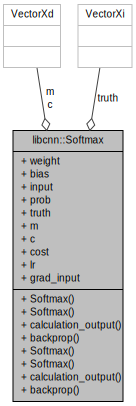
\includegraphics[width=208pt]{classlibcnn_1_1_softmax__coll__graph}
\end{center}
\end{figure}
\subsection*{\-Public \-Member \-Functions}
\begin{DoxyCompactItemize}
\item 
\hyperlink{classlibcnn_1_1_softmax_a1905addb7d4894b92ebb3c141040f7a1}{\-Softmax} (const \-Matrix\-Xd \&, const int \&, const \-Vector\-Xi \&, const double \&, const double \&)
\item 
\hyperlink{classlibcnn_1_1_softmax_aa43e90709ba3c5e44e5b7b435e54a902}{\-Softmax} (const \-Matrix\-Xd \&, const int \&, const \-Vector\-Xi \&, const double \&, const double \&, const \-Matrix\-Xd \&, const \-Matrix\-Xd \&)
\item 
void \hyperlink{classlibcnn_1_1_softmax_ae6af9e18ce2ab849d26b38a9d4a5be20}{calculation\-\_\-output} ()
\item 
void \hyperlink{classlibcnn_1_1_softmax_ad52de893453032d29c6fb3bca6e9f492}{backprop} (const double \&)
\item 
\hyperlink{classlibcnn_1_1_softmax_a1905addb7d4894b92ebb3c141040f7a1}{\-Softmax} (const \-Matrix\-Xd \&, const int \&, const \-Vector\-Xi \&, const double \&, const double \&)
\item 
\hyperlink{classlibcnn_1_1_softmax_aa43e90709ba3c5e44e5b7b435e54a902}{\-Softmax} (const \-Matrix\-Xd \&, const int \&, const \-Vector\-Xi \&, const double \&, const double \&, const \-Matrix\-Xd \&, const \-Matrix\-Xd \&)
\item 
void \hyperlink{classlibcnn_1_1_softmax_ae6af9e18ce2ab849d26b38a9d4a5be20}{calculation\-\_\-output} ()
\item 
void \hyperlink{classlibcnn_1_1_softmax_ad52de893453032d29c6fb3bca6e9f492}{backprop} (const double \&)
\end{DoxyCompactItemize}
\subsection*{\-Public \-Attributes}
\begin{DoxyCompactItemize}
\item 
\-Eigen\-::\-Matrix\-Xd \hyperlink{classlibcnn_1_1_softmax_a9904a3314f8b72c089cdfe5930f75445}{weight}
\item 
\-Eigen\-::\-Matrix\-Xd \hyperlink{classlibcnn_1_1_softmax_af7177b8068a5bb00b493684bd17e133e}{bias}
\item 
\-Eigen\-::\-Matrix\-Xd \hyperlink{classlibcnn_1_1_softmax_a6a7f3d59e90ecf66b9ddf437b452c780}{input}
\item 
\-Eigen\-::\-Matrix\-Xd \hyperlink{classlibcnn_1_1_softmax_a0d1f28abafbb3cddcf87defa87178ce4}{prob}
\item 
\-Eigen\-::\-Vector\-Xi \hyperlink{classlibcnn_1_1_softmax_ad2c468ea12679d111190c549fc46d8c1}{truth}
\item 
\-Eigen\-::\-Vector\-Xd \hyperlink{classlibcnn_1_1_softmax_a851740b9977df6ebc1dd3c672e367f56}{m}
\item 
\-Eigen\-::\-Vector\-Xd \hyperlink{classlibcnn_1_1_softmax_a89d340fbed0365db9c30dffafc492aca}{c}
\item 
double \hyperlink{classlibcnn_1_1_softmax_a13cbff525a19cea4f94836f5b439b2a7}{cost}
\item 
double \hyperlink{classlibcnn_1_1_softmax_a3995e5ba8bc5d766482735974b8eda92}{lr}
\item 
\-Eigen\-::\-Matrix\-Xd \hyperlink{classlibcnn_1_1_softmax_a3c4257681cef58ab58ca3601400ab098}{grad\-\_\-input}
\end{DoxyCompactItemize}


\subsection{\-Constructor \& \-Destructor \-Documentation}
\hypertarget{classlibcnn_1_1_softmax_a1905addb7d4894b92ebb3c141040f7a1}{\index{libcnn\-::\-Softmax@{libcnn\-::\-Softmax}!\-Softmax@{\-Softmax}}
\index{\-Softmax@{\-Softmax}!libcnn::Softmax@{libcnn\-::\-Softmax}}
\subsubsection[{\-Softmax}]{\setlength{\rightskip}{0pt plus 5cm}{\bf libcnn\-::\-Softmax\-::\-Softmax} (
\begin{DoxyParamCaption}
\item[{const \-Matrix\-Xd \&}]{cnn\-\_\-output, }
\item[{const int \&}]{\-Label\-\_\-number, }
\item[{const \-Vector\-Xi \&}]{ground\-\_\-truth, }
\item[{const double \&}]{w\-\_\-bound, }
\item[{const double \&}]{b\-\_\-bound}
\end{DoxyParamCaption}
)}}\label{classlibcnn_1_1_softmax_a1905addb7d4894b92ebb3c141040f7a1}


\-Here is the call graph for this function\-:
\nopagebreak
\begin{figure}[H]
\begin{center}
\leavevmode
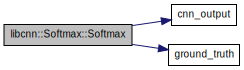
\includegraphics[width=316pt]{classlibcnn_1_1_softmax_a1905addb7d4894b92ebb3c141040f7a1_cgraph}
\end{center}
\end{figure}


\hypertarget{classlibcnn_1_1_softmax_aa43e90709ba3c5e44e5b7b435e54a902}{\index{libcnn\-::\-Softmax@{libcnn\-::\-Softmax}!\-Softmax@{\-Softmax}}
\index{\-Softmax@{\-Softmax}!libcnn::Softmax@{libcnn\-::\-Softmax}}
\subsubsection[{\-Softmax}]{\setlength{\rightskip}{0pt plus 5cm}{\bf libcnn\-::\-Softmax\-::\-Softmax} (
\begin{DoxyParamCaption}
\item[{const \-Matrix\-Xd \&}]{cnn\-\_\-output, }
\item[{const int \&}]{\-Label\-\_\-number, }
\item[{const \-Vector\-Xi \&}]{ground\-\_\-truth, }
\item[{const double \&}]{w\-\_\-bound, }
\item[{const double \&}]{b\-\_\-bound, }
\item[{const \-Matrix\-Xd \&}]{initial\-\_\-weight, }
\item[{const \-Matrix\-Xd \&}]{initial\-\_\-bias}
\end{DoxyParamCaption}
)}}\label{classlibcnn_1_1_softmax_aa43e90709ba3c5e44e5b7b435e54a902}


\-Here is the call graph for this function\-:
\nopagebreak
\begin{figure}[H]
\begin{center}
\leavevmode
\includegraphics[width=316pt]{classlibcnn_1_1_softmax_aa43e90709ba3c5e44e5b7b435e54a902_cgraph}
\end{center}
\end{figure}


\hypertarget{classlibcnn_1_1_softmax_a1905addb7d4894b92ebb3c141040f7a1}{\index{libcnn\-::\-Softmax@{libcnn\-::\-Softmax}!\-Softmax@{\-Softmax}}
\index{\-Softmax@{\-Softmax}!libcnn::Softmax@{libcnn\-::\-Softmax}}
\subsubsection[{\-Softmax}]{\setlength{\rightskip}{0pt plus 5cm}{\bf libcnn\-::\-Softmax\-::\-Softmax} (
\begin{DoxyParamCaption}
\item[{const \-Matrix\-Xd \&}]{, }
\item[{const int \&}]{, }
\item[{const \-Vector\-Xi \&}]{, }
\item[{const double \&}]{, }
\item[{const double \&}]{}
\end{DoxyParamCaption}
)}}\label{classlibcnn_1_1_softmax_a1905addb7d4894b92ebb3c141040f7a1}
\hypertarget{classlibcnn_1_1_softmax_aa43e90709ba3c5e44e5b7b435e54a902}{\index{libcnn\-::\-Softmax@{libcnn\-::\-Softmax}!\-Softmax@{\-Softmax}}
\index{\-Softmax@{\-Softmax}!libcnn::Softmax@{libcnn\-::\-Softmax}}
\subsubsection[{\-Softmax}]{\setlength{\rightskip}{0pt plus 5cm}{\bf libcnn\-::\-Softmax\-::\-Softmax} (
\begin{DoxyParamCaption}
\item[{const \-Matrix\-Xd \&}]{, }
\item[{const int \&}]{, }
\item[{const \-Vector\-Xi \&}]{, }
\item[{const double \&}]{, }
\item[{const double \&}]{, }
\item[{const \-Matrix\-Xd \&}]{, }
\item[{const \-Matrix\-Xd \&}]{}
\end{DoxyParamCaption}
)}}\label{classlibcnn_1_1_softmax_aa43e90709ba3c5e44e5b7b435e54a902}


\subsection{\-Member \-Function \-Documentation}
\hypertarget{classlibcnn_1_1_softmax_ad52de893453032d29c6fb3bca6e9f492}{\index{libcnn\-::\-Softmax@{libcnn\-::\-Softmax}!backprop@{backprop}}
\index{backprop@{backprop}!libcnn::Softmax@{libcnn\-::\-Softmax}}
\subsubsection[{backprop}]{\setlength{\rightskip}{0pt plus 5cm}void {\bf libcnn\-::\-Softmax\-::backprop} (
\begin{DoxyParamCaption}
\item[{const double \&}]{lr}
\end{DoxyParamCaption}
)}}\label{classlibcnn_1_1_softmax_ad52de893453032d29c6fb3bca6e9f492}
\hypertarget{classlibcnn_1_1_softmax_ad52de893453032d29c6fb3bca6e9f492}{\index{libcnn\-::\-Softmax@{libcnn\-::\-Softmax}!backprop@{backprop}}
\index{backprop@{backprop}!libcnn::Softmax@{libcnn\-::\-Softmax}}
\subsubsection[{backprop}]{\setlength{\rightskip}{0pt plus 5cm}void {\bf libcnn\-::\-Softmax\-::backprop} (
\begin{DoxyParamCaption}
\item[{const double \&}]{}
\end{DoxyParamCaption}
)}}\label{classlibcnn_1_1_softmax_ad52de893453032d29c6fb3bca6e9f492}
\hypertarget{classlibcnn_1_1_softmax_ae6af9e18ce2ab849d26b38a9d4a5be20}{\index{libcnn\-::\-Softmax@{libcnn\-::\-Softmax}!calculation\-\_\-output@{calculation\-\_\-output}}
\index{calculation\-\_\-output@{calculation\-\_\-output}!libcnn::Softmax@{libcnn\-::\-Softmax}}
\subsubsection[{calculation\-\_\-output}]{\setlength{\rightskip}{0pt plus 5cm}void {\bf libcnn\-::\-Softmax\-::calculation\-\_\-output} (
\begin{DoxyParamCaption}
{}
\end{DoxyParamCaption}
)}}\label{classlibcnn_1_1_softmax_ae6af9e18ce2ab849d26b38a9d4a5be20}
\hypertarget{classlibcnn_1_1_softmax_ae6af9e18ce2ab849d26b38a9d4a5be20}{\index{libcnn\-::\-Softmax@{libcnn\-::\-Softmax}!calculation\-\_\-output@{calculation\-\_\-output}}
\index{calculation\-\_\-output@{calculation\-\_\-output}!libcnn::Softmax@{libcnn\-::\-Softmax}}
\subsubsection[{calculation\-\_\-output}]{\setlength{\rightskip}{0pt plus 5cm}void {\bf libcnn\-::\-Softmax\-::calculation\-\_\-output} (
\begin{DoxyParamCaption}
{}
\end{DoxyParamCaption}
)}}\label{classlibcnn_1_1_softmax_ae6af9e18ce2ab849d26b38a9d4a5be20}


\subsection{\-Member \-Data \-Documentation}
\hypertarget{classlibcnn_1_1_softmax_af7177b8068a5bb00b493684bd17e133e}{\index{libcnn\-::\-Softmax@{libcnn\-::\-Softmax}!bias@{bias}}
\index{bias@{bias}!libcnn::Softmax@{libcnn\-::\-Softmax}}
\subsubsection[{bias}]{\setlength{\rightskip}{0pt plus 5cm}\-Eigen\-::\-Matrix\-Xd {\bf libcnn\-::\-Softmax\-::bias}}}\label{classlibcnn_1_1_softmax_af7177b8068a5bb00b493684bd17e133e}
\hypertarget{classlibcnn_1_1_softmax_a89d340fbed0365db9c30dffafc492aca}{\index{libcnn\-::\-Softmax@{libcnn\-::\-Softmax}!c@{c}}
\index{c@{c}!libcnn::Softmax@{libcnn\-::\-Softmax}}
\subsubsection[{c}]{\setlength{\rightskip}{0pt plus 5cm}\-Eigen\-::\-Vector\-Xd {\bf libcnn\-::\-Softmax\-::c}}}\label{classlibcnn_1_1_softmax_a89d340fbed0365db9c30dffafc492aca}
\hypertarget{classlibcnn_1_1_softmax_a13cbff525a19cea4f94836f5b439b2a7}{\index{libcnn\-::\-Softmax@{libcnn\-::\-Softmax}!cost@{cost}}
\index{cost@{cost}!libcnn::Softmax@{libcnn\-::\-Softmax}}
\subsubsection[{cost}]{\setlength{\rightskip}{0pt plus 5cm}double {\bf libcnn\-::\-Softmax\-::cost}}}\label{classlibcnn_1_1_softmax_a13cbff525a19cea4f94836f5b439b2a7}
\hypertarget{classlibcnn_1_1_softmax_a3c4257681cef58ab58ca3601400ab098}{\index{libcnn\-::\-Softmax@{libcnn\-::\-Softmax}!grad\-\_\-input@{grad\-\_\-input}}
\index{grad\-\_\-input@{grad\-\_\-input}!libcnn::Softmax@{libcnn\-::\-Softmax}}
\subsubsection[{grad\-\_\-input}]{\setlength{\rightskip}{0pt plus 5cm}\-Eigen\-::\-Matrix\-Xd {\bf libcnn\-::\-Softmax\-::grad\-\_\-input}}}\label{classlibcnn_1_1_softmax_a3c4257681cef58ab58ca3601400ab098}
\hypertarget{classlibcnn_1_1_softmax_a6a7f3d59e90ecf66b9ddf437b452c780}{\index{libcnn\-::\-Softmax@{libcnn\-::\-Softmax}!input@{input}}
\index{input@{input}!libcnn::Softmax@{libcnn\-::\-Softmax}}
\subsubsection[{input}]{\setlength{\rightskip}{0pt plus 5cm}\-Eigen\-::\-Matrix\-Xd {\bf libcnn\-::\-Softmax\-::input}}}\label{classlibcnn_1_1_softmax_a6a7f3d59e90ecf66b9ddf437b452c780}
\hypertarget{classlibcnn_1_1_softmax_a3995e5ba8bc5d766482735974b8eda92}{\index{libcnn\-::\-Softmax@{libcnn\-::\-Softmax}!lr@{lr}}
\index{lr@{lr}!libcnn::Softmax@{libcnn\-::\-Softmax}}
\subsubsection[{lr}]{\setlength{\rightskip}{0pt plus 5cm}double {\bf libcnn\-::\-Softmax\-::lr}}}\label{classlibcnn_1_1_softmax_a3995e5ba8bc5d766482735974b8eda92}
\hypertarget{classlibcnn_1_1_softmax_a851740b9977df6ebc1dd3c672e367f56}{\index{libcnn\-::\-Softmax@{libcnn\-::\-Softmax}!m@{m}}
\index{m@{m}!libcnn::Softmax@{libcnn\-::\-Softmax}}
\subsubsection[{m}]{\setlength{\rightskip}{0pt plus 5cm}\-Eigen\-::\-Vector\-Xd {\bf libcnn\-::\-Softmax\-::m}}}\label{classlibcnn_1_1_softmax_a851740b9977df6ebc1dd3c672e367f56}
\hypertarget{classlibcnn_1_1_softmax_a0d1f28abafbb3cddcf87defa87178ce4}{\index{libcnn\-::\-Softmax@{libcnn\-::\-Softmax}!prob@{prob}}
\index{prob@{prob}!libcnn::Softmax@{libcnn\-::\-Softmax}}
\subsubsection[{prob}]{\setlength{\rightskip}{0pt plus 5cm}\-Eigen\-::\-Matrix\-Xd {\bf libcnn\-::\-Softmax\-::prob}}}\label{classlibcnn_1_1_softmax_a0d1f28abafbb3cddcf87defa87178ce4}
\hypertarget{classlibcnn_1_1_softmax_ad2c468ea12679d111190c549fc46d8c1}{\index{libcnn\-::\-Softmax@{libcnn\-::\-Softmax}!truth@{truth}}
\index{truth@{truth}!libcnn::Softmax@{libcnn\-::\-Softmax}}
\subsubsection[{truth}]{\setlength{\rightskip}{0pt plus 5cm}\-Eigen\-::\-Vector\-Xi {\bf libcnn\-::\-Softmax\-::truth}}}\label{classlibcnn_1_1_softmax_ad2c468ea12679d111190c549fc46d8c1}
\hypertarget{classlibcnn_1_1_softmax_a9904a3314f8b72c089cdfe5930f75445}{\index{libcnn\-::\-Softmax@{libcnn\-::\-Softmax}!weight@{weight}}
\index{weight@{weight}!libcnn::Softmax@{libcnn\-::\-Softmax}}
\subsubsection[{weight}]{\setlength{\rightskip}{0pt plus 5cm}\-Eigen\-::\-Matrix\-Xd {\bf libcnn\-::\-Softmax\-::weight}}}\label{classlibcnn_1_1_softmax_a9904a3314f8b72c089cdfe5930f75445}


\-The documentation for this class was generated from the following files\-:\begin{DoxyCompactItemize}
\item 
gpu/include/\hyperlink{gpu_2include_2softmax__class_8h}{softmax\-\_\-class.\-h}\item 
include/\hyperlink{include_2softmax__class_8h}{softmax\-\_\-class.\-h}\item 
gpu/src/\hyperlink{gpu_2src_2softmax__class_8cpp}{softmax\-\_\-class.\-cpp}\item 
src/\hyperlink{src_2softmax__class_8cpp}{softmax\-\_\-class.\-cpp}\end{DoxyCompactItemize}

\chapter{\-File \-Documentation}
\input{_c_make_c_compiler_id_8c}
\input{_c_make_c_x_x_compiler_id_8cpp}
\input{gpu_2include_2conv__layer_8h}
\input{include_2conv__layer_8h}
\hypertarget{gpu_2include_2init__params_8h}{\section{gpu/include/init\-\_\-params.h \-File \-Reference}
\label{gpu_2include_2init__params_8h}\index{gpu/include/init\-\_\-params.\-h@{gpu/include/init\-\_\-params.\-h}}
}
{\ttfamily \#include $<$iostream$>$}\*
{\ttfamily \#include $<$\-Eigen/\-Dense$>$}\*
{\ttfamily \#include $<$vector$>$}\*
{\ttfamily \#include $<$string$>$}\*
\-Include dependency graph for init\-\_\-params.\-h\-:
\nopagebreak
\begin{figure}[H]
\begin{center}
\leavevmode
\includegraphics[width=344pt]{gpu_2include_2init__params_8h__incl}
\end{center}
\end{figure}
\subsection*{\-Namespaces}
\begin{DoxyCompactItemize}
\item 
namespace \hyperlink{namespacelibcnn}{libcnn}
\end{DoxyCompactItemize}
\subsection*{\-Functions}
\begin{DoxyCompactItemize}
\item 
void \hyperlink{namespacelibcnn_a2c5ccad2e675235e71fd5e5641ede4ae}{libcnn\-::get\-\_\-parameter} (vector$<$ \-Matrix\-Xd $>$ \&)
\end{DoxyCompactItemize}

\hypertarget{include_2init__params_8h}{\section{include/init\-\_\-params.h \-File \-Reference}
\label{include_2init__params_8h}\index{include/init\-\_\-params.\-h@{include/init\-\_\-params.\-h}}
}
{\ttfamily \#include $<$iostream$>$}\*
{\ttfamily \#include $<$\-Eigen/\-Dense$>$}\*
{\ttfamily \#include $<$vector$>$}\*
{\ttfamily \#include $<$string$>$}\*
\-Include dependency graph for init\-\_\-params.\-h\-:
\nopagebreak
\begin{figure}[H]
\begin{center}
\leavevmode
\includegraphics[width=344pt]{include_2init__params_8h__incl}
\end{center}
\end{figure}
\-This graph shows which files directly or indirectly include this file\-:
\nopagebreak
\begin{figure}[H]
\begin{center}
\leavevmode
\includegraphics[width=350pt]{include_2init__params_8h__dep__incl}
\end{center}
\end{figure}
\subsection*{\-Namespaces}
\begin{DoxyCompactItemize}
\item 
namespace \hyperlink{namespacelibcnn}{libcnn}
\end{DoxyCompactItemize}
\subsection*{\-Functions}
\begin{DoxyCompactItemize}
\item 
void \hyperlink{namespacelibcnn_a2c5ccad2e675235e71fd5e5641ede4ae}{libcnn\-::get\-\_\-parameter} (vector$<$ \-Matrix\-Xd $>$ \&)
\end{DoxyCompactItemize}

\input{gpu_2include_2load__data_8h}
\input{include_2load__data_8h}
\input{gpu_2include_2online__test_8h}
\input{include_2online__test_8h}
\hypertarget{gpu_2include_2pool_8h}{\section{gpu/include/pool.h \-File \-Reference}
\label{gpu_2include_2pool_8h}\index{gpu/include/pool.\-h@{gpu/include/pool.\-h}}
}
{\ttfamily \#include $<$iostream$>$}\*
{\ttfamily \#include $<$\-Eigen/\-Dense$>$}\*
{\ttfamily \#include $<$vector$>$}\*
{\ttfamily \#include $<$cmath$>$}\*
{\ttfamily \#include $<$string$>$}\*
\-Include dependency graph for pool.\-h\-:
\nopagebreak
\begin{figure}[H]
\begin{center}
\leavevmode
\includegraphics[width=350pt]{gpu_2include_2pool_8h__incl}
\end{center}
\end{figure}
\subsection*{\-Classes}
\begin{DoxyCompactItemize}
\item 
class \hyperlink{classlibcnn_1_1_pool}{libcnn\-::\-Pool}
\end{DoxyCompactItemize}
\subsection*{\-Namespaces}
\begin{DoxyCompactItemize}
\item 
namespace \hyperlink{namespacelibcnn}{libcnn}
\end{DoxyCompactItemize}

\hypertarget{include_2pool_8h}{\section{include/pool.h \-File \-Reference}
\label{include_2pool_8h}\index{include/pool.\-h@{include/pool.\-h}}
}
{\ttfamily \#include $<$iostream$>$}\*
{\ttfamily \#include $<$\-Eigen/\-Dense$>$}\*
{\ttfamily \#include $<$vector$>$}\*
{\ttfamily \#include $<$cmath$>$}\*
{\ttfamily \#include $<$string$>$}\*
\-Include dependency graph for pool.\-h\-:
\nopagebreak
\begin{figure}[H]
\begin{center}
\leavevmode
\includegraphics[width=350pt]{include_2pool_8h__incl}
\end{center}
\end{figure}
\-This graph shows which files directly or indirectly include this file\-:
\nopagebreak
\begin{figure}[H]
\begin{center}
\leavevmode
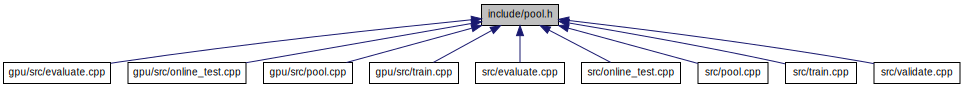
\includegraphics[width=350pt]{include_2pool_8h__dep__incl}
\end{center}
\end{figure}
\subsection*{\-Classes}
\begin{DoxyCompactItemize}
\item 
class \hyperlink{classlibcnn_1_1_pool}{libcnn\-::\-Pool}
\end{DoxyCompactItemize}
\subsection*{\-Namespaces}
\begin{DoxyCompactItemize}
\item 
namespace \hyperlink{namespacelibcnn}{libcnn}
\end{DoxyCompactItemize}

\input{gpu_2include_2preprocess_8h}
\input{include_2preprocess_8h}
\input{gpu_2include_2rand__initialize_8h}
\input{include_2rand__initialize_8h}
\hypertarget{gpu_2include_2save__params_8h}{\section{gpu/include/save\-\_\-params.h \-File \-Reference}
\label{gpu_2include_2save__params_8h}\index{gpu/include/save\-\_\-params.\-h@{gpu/include/save\-\_\-params.\-h}}
}
{\ttfamily \#include $<$iostream$>$}\*
{\ttfamily \#include $<$\-Eigen/\-Dense$>$}\*
{\ttfamily \#include $<$vector$>$}\*
\-Include dependency graph for save\-\_\-params.\-h\-:
\nopagebreak
\begin{figure}[H]
\begin{center}
\leavevmode
\includegraphics[width=286pt]{gpu_2include_2save__params_8h__incl}
\end{center}
\end{figure}
\subsection*{\-Namespaces}
\begin{DoxyCompactItemize}
\item 
namespace \hyperlink{namespacelibcnn}{libcnn}
\end{DoxyCompactItemize}
\subsection*{\-Functions}
\begin{DoxyCompactItemize}
\item 
void \hyperlink{namespacelibcnn_a35fa40f645f5fe20b4cc8d878b1e0c10}{libcnn\-::print\-\_\-params} (vector$<$ vector$<$ \-Matrix\-Xd $>$ $>$ \&, vector$<$ \-Matrix\-Xd $>$ \&, vector$<$ \-Matrix\-Xd $>$ \&, vector$<$ \-Matrix\-Xd $>$ \&, vector$<$ \-Matrix\-Xd $>$ \&, \-Matrix\-Xd \&, \-Matrix\-Xd \&, \-Matrix\-Xd \&, \-Matrix\-Xd \&, \-Matrix\-Xd \&)
\end{DoxyCompactItemize}

\input{include_2save__params_8h}
\input{gpu_2include_2softmax__class_8h}
\input{include_2softmax__class_8h}
\hypertarget{gpu_2src_2conv__layer_8cpp}{\section{gpu/src/conv\-\_\-layer.cpp \-File \-Reference}
\label{gpu_2src_2conv__layer_8cpp}\index{gpu/src/conv\-\_\-layer.\-cpp@{gpu/src/conv\-\_\-layer.\-cpp}}
}
{\ttfamily \#include \char`\"{}conv\-\_\-layer.\-h\char`\"{}}\*
{\ttfamily \#include $<$\-Eigen/\-Dense$>$}\*
{\ttfamily \#include $<$iostream$>$}\*
{\ttfamily \#include $<$vector$>$}\*
{\ttfamily \#include $<$cmath$>$}\*
{\ttfamily \#include $<$ctime$>$}\*
{\ttfamily \#include $<$string$>$}\*
{\ttfamily \#include $<$stdexcept$>$}\*
{\ttfamily \#include $<$sys/time.\-h$>$}\*
{\ttfamily \#include $<$omp.\-h$>$}\*
\-Include dependency graph for conv\-\_\-layer.\-cpp\-:
\nopagebreak
\begin{figure}[H]
\begin{center}
\leavevmode
\includegraphics[width=350pt]{gpu_2src_2conv__layer_8cpp__incl}
\end{center}
\end{figure}
\subsection*{\-Namespaces}
\begin{DoxyCompactItemize}
\item 
namespace \hyperlink{namespacelibcnn}{libcnn}
\end{DoxyCompactItemize}
\subsection*{\-Functions}
\begin{DoxyCompactItemize}
\item 
void \hyperlink{namespacelibcnn_a55bbe6e5488b8a038e5708a32d233090}{libcnn\-::get\-\_\-feature\-\_\-vector} (const vector$<$ vector$<$ \-Matrix\-Xd $>$ $>$ \&, \-Matrix\-Xd \&)
\item 
void \hyperlink{namespacelibcnn_a78ed8e63be87c4d06bb363af95ce62ec}{libcnn\-::softmax2conv} (const \-Matrix\-Xd \&, const int \&, const int \&, const int \&, vector$<$ vector$<$ \-Matrix\-Xd $>$ $>$ \&)
\end{DoxyCompactItemize}

\input{src_2conv__layer_8cpp}
\hypertarget{gpu_2src_2evaluate_8cpp}{\section{gpu/src/evaluate.cpp \-File \-Reference}
\label{gpu_2src_2evaluate_8cpp}\index{gpu/src/evaluate.\-cpp@{gpu/src/evaluate.\-cpp}}
}
{\ttfamily \#include $<$iostream$>$}\*
{\ttfamily \#include $<$\-Eigen/\-Dense$>$}\*
{\ttfamily \#include $<$vector$>$}\*
{\ttfamily \#include $<$fstream$>$}\*
{\ttfamily \#include $<$string$>$}\*
{\ttfamily \#include \char`\"{}conv\-\_\-layer.\-h\char`\"{}}\*
{\ttfamily \#include \char`\"{}softmax\-\_\-class.\-h\char`\"{}}\*
{\ttfamily \#include \char`\"{}pool.\-h\char`\"{}}\*
{\ttfamily \#include \char`\"{}load\-\_\-data.\-h\char`\"{}}\*
\-Include dependency graph for evaluate.\-cpp\-:
\nopagebreak
\begin{figure}[H]
\begin{center}
\leavevmode
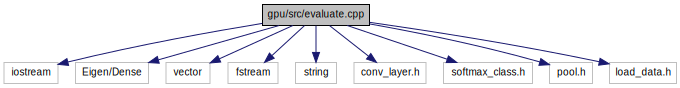
\includegraphics[width=350pt]{gpu_2src_2evaluate_8cpp__incl}
\end{center}
\end{figure}
\subsection*{\-Functions}
\begin{DoxyCompactItemize}
\item 
void \hyperlink{gpu_2src_2evaluate_8cpp_a640eb3c435abcfe65e13558fc738b915}{evaluate} ()
\item 
int \hyperlink{gpu_2src_2evaluate_8cpp_ae66f6b31b5ad750f1fe042a706a4e3d4}{main} ()
\end{DoxyCompactItemize}


\subsection{\-Function \-Documentation}
\hypertarget{gpu_2src_2evaluate_8cpp_a640eb3c435abcfe65e13558fc738b915}{\index{gpu/src/evaluate.\-cpp@{gpu/src/evaluate.\-cpp}!evaluate@{evaluate}}
\index{evaluate@{evaluate}!gpu/src/evaluate.cpp@{gpu/src/evaluate.\-cpp}}
\subsubsection[{evaluate}]{\setlength{\rightskip}{0pt plus 5cm}void {\bf evaluate} (
\begin{DoxyParamCaption}
{}
\end{DoxyParamCaption}
)}}\label{gpu_2src_2evaluate_8cpp_a640eb3c435abcfe65e13558fc738b915}
\hypertarget{gpu_2src_2evaluate_8cpp_ae66f6b31b5ad750f1fe042a706a4e3d4}{\index{gpu/src/evaluate.\-cpp@{gpu/src/evaluate.\-cpp}!main@{main}}
\index{main@{main}!gpu/src/evaluate.cpp@{gpu/src/evaluate.\-cpp}}
\subsubsection[{main}]{\setlength{\rightskip}{0pt plus 5cm}int {\bf main} (
\begin{DoxyParamCaption}
{}
\end{DoxyParamCaption}
)}}\label{gpu_2src_2evaluate_8cpp_ae66f6b31b5ad750f1fe042a706a4e3d4}


\-Here is the call graph for this function\-:
\nopagebreak
\begin{figure}[H]
\begin{center}
\leavevmode
\includegraphics[width=208pt]{gpu_2src_2evaluate_8cpp_ae66f6b31b5ad750f1fe042a706a4e3d4_cgraph}
\end{center}
\end{figure}



\hypertarget{src_2evaluate_8cpp}{\section{src/evaluate.cpp \-File \-Reference}
\label{src_2evaluate_8cpp}\index{src/evaluate.\-cpp@{src/evaluate.\-cpp}}
}
{\ttfamily \#include $<$iostream$>$}\*
{\ttfamily \#include $<$\-Eigen/\-Dense$>$}\*
{\ttfamily \#include $<$vector$>$}\*
{\ttfamily \#include $<$fstream$>$}\*
{\ttfamily \#include $<$string$>$}\*
{\ttfamily \#include \char`\"{}conv\-\_\-layer.\-h\char`\"{}}\*
{\ttfamily \#include \char`\"{}softmax\-\_\-class.\-h\char`\"{}}\*
{\ttfamily \#include \char`\"{}pool.\-h\char`\"{}}\*
{\ttfamily \#include \char`\"{}load\-\_\-data.\-h\char`\"{}}\*
\-Include dependency graph for evaluate.\-cpp\-:
\nopagebreak
\begin{figure}[H]
\begin{center}
\leavevmode
\includegraphics[width=350pt]{src_2evaluate_8cpp__incl}
\end{center}
\end{figure}
\subsection*{\-Functions}
\begin{DoxyCompactItemize}
\item 
void \hyperlink{src_2evaluate_8cpp_a640eb3c435abcfe65e13558fc738b915}{evaluate} ()
\item 
int \hyperlink{src_2evaluate_8cpp_ae66f6b31b5ad750f1fe042a706a4e3d4}{main} ()
\end{DoxyCompactItemize}


\subsection{\-Function \-Documentation}
\hypertarget{src_2evaluate_8cpp_a640eb3c435abcfe65e13558fc738b915}{\index{src/evaluate.\-cpp@{src/evaluate.\-cpp}!evaluate@{evaluate}}
\index{evaluate@{evaluate}!src/evaluate.cpp@{src/evaluate.\-cpp}}
\subsubsection[{evaluate}]{\setlength{\rightskip}{0pt plus 5cm}void {\bf evaluate} (
\begin{DoxyParamCaption}
{}
\end{DoxyParamCaption}
)}}\label{src_2evaluate_8cpp_a640eb3c435abcfe65e13558fc738b915}
\hypertarget{src_2evaluate_8cpp_ae66f6b31b5ad750f1fe042a706a4e3d4}{\index{src/evaluate.\-cpp@{src/evaluate.\-cpp}!main@{main}}
\index{main@{main}!src/evaluate.cpp@{src/evaluate.\-cpp}}
\subsubsection[{main}]{\setlength{\rightskip}{0pt plus 5cm}int {\bf main} (
\begin{DoxyParamCaption}
{}
\end{DoxyParamCaption}
)}}\label{src_2evaluate_8cpp_ae66f6b31b5ad750f1fe042a706a4e3d4}


\-Here is the call graph for this function\-:
\nopagebreak
\begin{figure}[H]
\begin{center}
\leavevmode
\includegraphics[width=208pt]{src_2evaluate_8cpp_ae66f6b31b5ad750f1fe042a706a4e3d4_cgraph}
\end{center}
\end{figure}



\hypertarget{gpu_2src_2init__params_8cpp}{\section{gpu/src/init\-\_\-params.cpp \-File \-Reference}
\label{gpu_2src_2init__params_8cpp}\index{gpu/src/init\-\_\-params.\-cpp@{gpu/src/init\-\_\-params.\-cpp}}
}
{\ttfamily \#include $<$iostream$>$}\*
{\ttfamily \#include $<$fstream$>$}\*
{\ttfamily \#include $<$string$>$}\*
{\ttfamily \#include $<$vector$>$}\*
{\ttfamily \#include $<$\-Eigen/\-Dense$>$}\*
{\ttfamily \#include $<$sstream$>$}\*
{\ttfamily \#include \char`\"{}init\-\_\-params.\-h\char`\"{}}\*
\-Include dependency graph for init\-\_\-params.\-cpp\-:
\nopagebreak
\begin{figure}[H]
\begin{center}
\leavevmode
\includegraphics[width=350pt]{gpu_2src_2init__params_8cpp__incl}
\end{center}
\end{figure}
\subsection*{\-Namespaces}
\begin{DoxyCompactItemize}
\item 
namespace \hyperlink{namespacelibcnn}{libcnn}
\end{DoxyCompactItemize}
\subsection*{\-Defines}
\begin{DoxyCompactItemize}
\item 
\#define \hyperlink{gpu_2src_2init__params_8cpp_aae9a32fb4ed60a2b23dd7eca52e8e627}{\-K\-E\-R\-N\-E\-L\-\_\-\-S\-I\-Z\-E}~7
\end{DoxyCompactItemize}
\subsection*{\-Functions}
\begin{DoxyCompactItemize}
\item 
void \hyperlink{namespacelibcnn_a2c5ccad2e675235e71fd5e5641ede4ae}{libcnn\-::get\-\_\-parameter} (vector$<$ \-Matrix\-Xd $>$ \&)
\end{DoxyCompactItemize}


\subsection{\-Define \-Documentation}
\hypertarget{gpu_2src_2init__params_8cpp_aae9a32fb4ed60a2b23dd7eca52e8e627}{\index{gpu/src/init\-\_\-params.\-cpp@{gpu/src/init\-\_\-params.\-cpp}!\-K\-E\-R\-N\-E\-L\-\_\-\-S\-I\-Z\-E@{\-K\-E\-R\-N\-E\-L\-\_\-\-S\-I\-Z\-E}}
\index{\-K\-E\-R\-N\-E\-L\-\_\-\-S\-I\-Z\-E@{\-K\-E\-R\-N\-E\-L\-\_\-\-S\-I\-Z\-E}!gpu/src/init_params.cpp@{gpu/src/init\-\_\-params.\-cpp}}
\subsubsection[{\-K\-E\-R\-N\-E\-L\-\_\-\-S\-I\-Z\-E}]{\setlength{\rightskip}{0pt plus 5cm}\#define {\bf \-K\-E\-R\-N\-E\-L\-\_\-\-S\-I\-Z\-E}~7}}\label{gpu_2src_2init__params_8cpp_aae9a32fb4ed60a2b23dd7eca52e8e627}

\hypertarget{src_2init__params_8cpp}{\section{src/init\-\_\-params.cpp \-File \-Reference}
\label{src_2init__params_8cpp}\index{src/init\-\_\-params.\-cpp@{src/init\-\_\-params.\-cpp}}
}
{\ttfamily \#include $<$iostream$>$}\*
{\ttfamily \#include $<$fstream$>$}\*
{\ttfamily \#include $<$string$>$}\*
{\ttfamily \#include $<$vector$>$}\*
{\ttfamily \#include $<$\-Eigen/\-Dense$>$}\*
{\ttfamily \#include $<$sstream$>$}\*
{\ttfamily \#include \char`\"{}init\-\_\-params.\-h\char`\"{}}\*
\-Include dependency graph for init\-\_\-params.\-cpp\-:
\nopagebreak
\begin{figure}[H]
\begin{center}
\leavevmode
\includegraphics[width=350pt]{src_2init__params_8cpp__incl}
\end{center}
\end{figure}
\subsection*{\-Namespaces}
\begin{DoxyCompactItemize}
\item 
namespace \hyperlink{namespacelibcnn}{libcnn}
\end{DoxyCompactItemize}
\subsection*{\-Defines}
\begin{DoxyCompactItemize}
\item 
\#define \hyperlink{src_2init__params_8cpp_aae9a32fb4ed60a2b23dd7eca52e8e627}{\-K\-E\-R\-N\-E\-L\-\_\-\-S\-I\-Z\-E}~7
\end{DoxyCompactItemize}
\subsection*{\-Functions}
\begin{DoxyCompactItemize}
\item 
void \hyperlink{namespacelibcnn_a2c5ccad2e675235e71fd5e5641ede4ae}{libcnn\-::get\-\_\-parameter} (vector$<$ \-Matrix\-Xd $>$ \&)
\end{DoxyCompactItemize}


\subsection{\-Define \-Documentation}
\hypertarget{src_2init__params_8cpp_aae9a32fb4ed60a2b23dd7eca52e8e627}{\index{src/init\-\_\-params.\-cpp@{src/init\-\_\-params.\-cpp}!\-K\-E\-R\-N\-E\-L\-\_\-\-S\-I\-Z\-E@{\-K\-E\-R\-N\-E\-L\-\_\-\-S\-I\-Z\-E}}
\index{\-K\-E\-R\-N\-E\-L\-\_\-\-S\-I\-Z\-E@{\-K\-E\-R\-N\-E\-L\-\_\-\-S\-I\-Z\-E}!src/init_params.cpp@{src/init\-\_\-params.\-cpp}}
\subsubsection[{\-K\-E\-R\-N\-E\-L\-\_\-\-S\-I\-Z\-E}]{\setlength{\rightskip}{0pt plus 5cm}\#define {\bf \-K\-E\-R\-N\-E\-L\-\_\-\-S\-I\-Z\-E}~7}}\label{src_2init__params_8cpp_aae9a32fb4ed60a2b23dd7eca52e8e627}

\input{gpu_2src_2load__data_8cpp}
\hypertarget{src_2load__data_8cpp}{\section{src/load\-\_\-data.cpp \-File \-Reference}
\label{src_2load__data_8cpp}\index{src/load\-\_\-data.\-cpp@{src/load\-\_\-data.\-cpp}}
}
{\ttfamily \#include $<$sys/types.\-h$>$}\*
{\ttfamily \#include $<$dirent.\-h$>$}\*
{\ttfamily \#include $<$errno.\-h$>$}\*
{\ttfamily \#include $<$vector$>$}\*
{\ttfamily \#include $<$string.\-h$>$}\*
{\ttfamily \#include $<$iostream$>$}\*
{\ttfamily \#include $<$stdlib.\-h$>$}\*
{\ttfamily \#include $<$fstream$>$}\*
{\ttfamily \#include $<$\-Eigen/\-Dense$>$}\*
{\ttfamily \#include $<$cassert$>$}\*
{\ttfamily \#include $<$algorithm$>$}\*
{\ttfamily \#include $<$string$>$}\*
\-Include dependency graph for load\-\_\-data.\-cpp\-:
\nopagebreak
\begin{figure}[H]
\begin{center}
\leavevmode
\includegraphics[width=350pt]{src_2load__data_8cpp__incl}
\end{center}
\end{figure}
\subsection*{\-Functions}
\begin{DoxyCompactItemize}
\item 
void \hyperlink{src_2load__data_8cpp_afbad2e91730f993e296f166a8f89aa9b}{getdir} (const string \&\hyperlink{yaml__t__load_8cpp_a7f01c047eb310166e695d4232ebd1fae}{dir}, vector$<$ string $>$ \&files)
\item 
void \hyperlink{src_2load__data_8cpp_a39a205061173088b2222b1d550a8787c}{read\-\_\-image\-\_\-files} (const string \&\hyperlink{yaml__t__load_8cpp_a7f01c047eb310166e695d4232ebd1fae}{dir}, std\-::vector$<$ vector$<$ \-Matrix\-Xd $>$ $>$ \&vvm, const int \&image\-\_\-row\-\_\-dim, const int \&image\-\_\-col\-\_\-dim, const int \&start, const int \&image\-\_\-number)
\item 
void \hyperlink{src_2load__data_8cpp_a8f84dc0bbc3acab545f50ce4899348e3}{read\-\_\-label\-\_\-files} (const string \&\hyperlink{yaml__t__load_8cpp_a7f01c047eb310166e695d4232ebd1fae}{dir}, \-Vector\-Xi \&m, const int \&image\-\_\-row\-\_\-dim, const int \&image\-\_\-col\-\_\-dim, const int \&start, const int \&image\-\_\-number, const string \&data\-\_\-mode)
\item 
void \hyperlink{src_2load__data_8cpp_ac599c564730d396dcd8eaf64c9878dcf}{read\-\_\-markov\-\_\-files} (const string \&dir\-\_\-name, \-Matrix\-Xd \&markov)
\end{DoxyCompactItemize}


\subsection{\-Function \-Documentation}
\hypertarget{src_2load__data_8cpp_afbad2e91730f993e296f166a8f89aa9b}{\index{src/load\-\_\-data.\-cpp@{src/load\-\_\-data.\-cpp}!getdir@{getdir}}
\index{getdir@{getdir}!src/load_data.cpp@{src/load\-\_\-data.\-cpp}}
\subsubsection[{getdir}]{\setlength{\rightskip}{0pt plus 5cm}void {\bf getdir} (
\begin{DoxyParamCaption}
\item[{const string \&}]{dir, }
\item[{vector$<$ string $>$ \&}]{files}
\end{DoxyParamCaption}
)}}\label{src_2load__data_8cpp_afbad2e91730f993e296f166a8f89aa9b}
\hypertarget{src_2load__data_8cpp_a39a205061173088b2222b1d550a8787c}{\index{src/load\-\_\-data.\-cpp@{src/load\-\_\-data.\-cpp}!read\-\_\-image\-\_\-files@{read\-\_\-image\-\_\-files}}
\index{read\-\_\-image\-\_\-files@{read\-\_\-image\-\_\-files}!src/load_data.cpp@{src/load\-\_\-data.\-cpp}}
\subsubsection[{read\-\_\-image\-\_\-files}]{\setlength{\rightskip}{0pt plus 5cm}void {\bf read\-\_\-image\-\_\-files} (
\begin{DoxyParamCaption}
\item[{const string \&}]{dir, }
\item[{std\-::vector$<$ vector$<$ \-Matrix\-Xd $>$ $>$ \&}]{vvm, }
\item[{const int \&}]{image\-\_\-row\-\_\-dim, }
\item[{const int \&}]{image\-\_\-col\-\_\-dim, }
\item[{const int \&}]{start, }
\item[{const int \&}]{image\-\_\-number}
\end{DoxyParamCaption}
)}}\label{src_2load__data_8cpp_a39a205061173088b2222b1d550a8787c}


\-Here is the call graph for this function\-:
\nopagebreak
\begin{figure}[H]
\begin{center}
\leavevmode
\includegraphics[width=248pt]{src_2load__data_8cpp_a39a205061173088b2222b1d550a8787c_cgraph}
\end{center}
\end{figure}


\hypertarget{src_2load__data_8cpp_a8f84dc0bbc3acab545f50ce4899348e3}{\index{src/load\-\_\-data.\-cpp@{src/load\-\_\-data.\-cpp}!read\-\_\-label\-\_\-files@{read\-\_\-label\-\_\-files}}
\index{read\-\_\-label\-\_\-files@{read\-\_\-label\-\_\-files}!src/load_data.cpp@{src/load\-\_\-data.\-cpp}}
\subsubsection[{read\-\_\-label\-\_\-files}]{\setlength{\rightskip}{0pt plus 5cm}void {\bf read\-\_\-label\-\_\-files} (
\begin{DoxyParamCaption}
\item[{const string \&}]{dir, }
\item[{\-Vector\-Xi \&}]{m, }
\item[{const int \&}]{image\-\_\-row\-\_\-dim, }
\item[{const int \&}]{image\-\_\-col\-\_\-dim, }
\item[{const int \&}]{start, }
\item[{const int \&}]{image\-\_\-number, }
\item[{const string \&}]{data\-\_\-mode}
\end{DoxyParamCaption}
)}}\label{src_2load__data_8cpp_a8f84dc0bbc3acab545f50ce4899348e3}


\-Here is the call graph for this function\-:
\nopagebreak
\begin{figure}[H]
\begin{center}
\leavevmode
\includegraphics[width=242pt]{src_2load__data_8cpp_a8f84dc0bbc3acab545f50ce4899348e3_cgraph}
\end{center}
\end{figure}


\hypertarget{src_2load__data_8cpp_ac599c564730d396dcd8eaf64c9878dcf}{\index{src/load\-\_\-data.\-cpp@{src/load\-\_\-data.\-cpp}!read\-\_\-markov\-\_\-files@{read\-\_\-markov\-\_\-files}}
\index{read\-\_\-markov\-\_\-files@{read\-\_\-markov\-\_\-files}!src/load_data.cpp@{src/load\-\_\-data.\-cpp}}
\subsubsection[{read\-\_\-markov\-\_\-files}]{\setlength{\rightskip}{0pt plus 5cm}void {\bf read\-\_\-markov\-\_\-files} (
\begin{DoxyParamCaption}
\item[{const string \&}]{dir\-\_\-name, }
\item[{\-Matrix\-Xd \&}]{markov}
\end{DoxyParamCaption}
)}}\label{src_2load__data_8cpp_ac599c564730d396dcd8eaf64c9878dcf}

\hypertarget{gpu_2src_2markov__1_8py}{\section{gpu/src/markov\-\_\-1.py \-File \-Reference}
\label{gpu_2src_2markov__1_8py}\index{gpu/src/markov\-\_\-1.\-py@{gpu/src/markov\-\_\-1.\-py}}
}
\subsection*{\-Namespaces}
\begin{DoxyCompactItemize}
\item 
namespace \hyperlink{namespacemarkov__1}{markov\-\_\-1}
\end{DoxyCompactItemize}
\subsection*{\-Variables}
\begin{DoxyCompactItemize}
\item 
float \hyperlink{namespacemarkov__1_a4a3eda3678257ab2cf6f06891c5ec22c}{markov\-\_\-1.\-roe} = 0.\-9999
\item 
list \hyperlink{namespacemarkov__1_ac6e549cf6d4d6df355d884b67fb19851}{markov\-\_\-1.\-roe\-\_\-list} = \mbox{[}$\,$\mbox{]}
\item 
int \hyperlink{namespacemarkov__1_a8134563a0c42390906c8914ad337e9d8}{markov\-\_\-1.\-data\-\_\-dimension} = 64
\item 
tuple \hyperlink{namespacemarkov__1_a7cc4d10a876ec07da21dbfd4d28e8684}{markov\-\_\-1.\-covariance\-\_\-matrix} = toeplitz(roe\-\_\-list, roe\-\_\-list)
\item 
\hyperlink{namespacemarkov__1_a3744683663f02bff5cf245a674ab9b32}{markov\-\_\-1.\-Data\-Out} = e\-\_\-vecs
\end{DoxyCompactItemize}

\input{src_2markov__1_8py}
\input{gpu_2src_2online__test_8cpp}
\hypertarget{src_2online__test_8cpp}{\section{src/online\-\_\-test.cpp \-File \-Reference}
\label{src_2online__test_8cpp}\index{src/online\-\_\-test.\-cpp@{src/online\-\_\-test.\-cpp}}
}
{\ttfamily \#include $<$iostream$>$}\*
{\ttfamily \#include $<$\-Eigen/\-Dense$>$}\*
{\ttfamily \#include $<$vector$>$}\*
{\ttfamily \#include \char`\"{}online\-\_\-test.\-h\char`\"{}}\*
{\ttfamily \#include \char`\"{}conv\-\_\-layer.\-h\char`\"{}}\*
{\ttfamily \#include \char`\"{}pool.\-h\char`\"{}}\*
{\ttfamily \#include \char`\"{}softmax\-\_\-class.\-h\char`\"{}}\*
\-Include dependency graph for online\-\_\-test.\-cpp\-:
\nopagebreak
\begin{figure}[H]
\begin{center}
\leavevmode
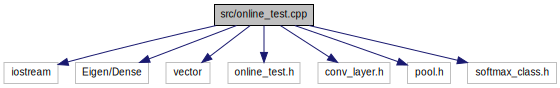
\includegraphics[width=350pt]{src_2online__test_8cpp__incl}
\end{center}
\end{figure}
\subsection*{\-Namespaces}
\begin{DoxyCompactItemize}
\item 
namespace \hyperlink{namespacelibcnn}{libcnn}
\end{DoxyCompactItemize}
\subsection*{\-Functions}
\begin{DoxyCompactItemize}
\item 
void \hyperlink{namespacelibcnn_a493fb452cedcc704e189ad1a3656c0ad}{libcnn\-::online\-\_\-test} (const vector$<$ vector$<$ \-Matrix\-Xd $>$ $>$ \&, const \-Vector\-Xi \&, const vector$<$ \-Matrix\-Xd $>$ \&, const \-Matrix\-Xd \&, const vector$<$ \-Matrix\-Xd $>$ \&, const \-Matrix\-Xd \&, const vector$<$ \-Matrix\-Xd $>$ \&, const \-Matrix\-Xd \&, const \-Matrix\-Xd \&, const \-Matrix\-Xd \&, const int \&, const int \&, const int \&, const int \&, const int \&)
\end{DoxyCompactItemize}

\hypertarget{gpu_2src_2pool_8cpp}{\section{gpu/src/pool.cpp \-File \-Reference}
\label{gpu_2src_2pool_8cpp}\index{gpu/src/pool.\-cpp@{gpu/src/pool.\-cpp}}
}
{\ttfamily \#include $<$iostream$>$}\*
{\ttfamily \#include $<$\-Eigen/\-Dense$>$}\*
{\ttfamily \#include $<$vector$>$}\*
{\ttfamily \#include $<$cmath$>$}\*
{\ttfamily \#include $<$string$>$}\*
{\ttfamily \#include \char`\"{}pool.\-h\char`\"{}}\*
\-Include dependency graph for pool.\-cpp\-:
\nopagebreak
\begin{figure}[H]
\begin{center}
\leavevmode
\includegraphics[width=350pt]{gpu_2src_2pool_8cpp__incl}
\end{center}
\end{figure}
\subsection*{\-Namespaces}
\begin{DoxyCompactItemize}
\item 
namespace \hyperlink{namespacelibcnn}{libcnn}
\end{DoxyCompactItemize}

\hypertarget{src_2pool_8cpp}{\section{src/pool.cpp \-File \-Reference}
\label{src_2pool_8cpp}\index{src/pool.\-cpp@{src/pool.\-cpp}}
}
{\ttfamily \#include $<$iostream$>$}\*
{\ttfamily \#include $<$\-Eigen/\-Dense$>$}\*
{\ttfamily \#include $<$vector$>$}\*
{\ttfamily \#include $<$cmath$>$}\*
{\ttfamily \#include $<$string$>$}\*
{\ttfamily \#include \char`\"{}pool.\-h\char`\"{}}\*
\-Include dependency graph for pool.\-cpp\-:
\nopagebreak
\begin{figure}[H]
\begin{center}
\leavevmode
\includegraphics[width=350pt]{src_2pool_8cpp__incl}
\end{center}
\end{figure}
\subsection*{\-Namespaces}
\begin{DoxyCompactItemize}
\item 
namespace \hyperlink{namespacelibcnn}{libcnn}
\end{DoxyCompactItemize}

\input{gpu_2src_2preprocess_8cpp}
\input{src_2preprocess_8cpp}
\input{gpu_2src_2rand__initialize_8cpp}
\input{src_2rand__initialize_8cpp}
\hypertarget{gpu_2src_2read__dat__file_8cpp}{\section{gpu/src/read\-\_\-dat\-\_\-file.cpp \-File \-Reference}
\label{gpu_2src_2read__dat__file_8cpp}\index{gpu/src/read\-\_\-dat\-\_\-file.\-cpp@{gpu/src/read\-\_\-dat\-\_\-file.\-cpp}}
}
{\ttfamily \#include $<$iostream$>$}\*
{\ttfamily \#include $<$fstream$>$}\*
{\ttfamily \#include $<$\-Eigen/\-Dense$>$}\*
{\ttfamily \#include $<$stdlib.\-h$>$}\*
{\ttfamily \#include $<$sstream$>$}\*
{\ttfamily \#include $<$cassert$>$}\*
{\ttfamily \#include $<$vector$>$}\*
\-Include dependency graph for read\-\_\-dat\-\_\-file.\-cpp\-:
\nopagebreak
\begin{figure}[H]
\begin{center}
\leavevmode
\includegraphics[width=350pt]{gpu_2src_2read__dat__file_8cpp__incl}
\end{center}
\end{figure}
\subsection*{\-Functions}
\begin{DoxyCompactItemize}
\item 
double \hyperlink{gpu_2src_2read__dat__file_8cpp_afe0bc81c124c80ed6a71504722cbecaf}{string\-\_\-to\-\_\-double} (string \&\hyperlink{get__klt__kernels_8m_a3691308f2a4c2f6983f2880d32e29c84}{s})
\item 
int \hyperlink{gpu_2src_2read__dat__file_8cpp_a0ddf1224851353fc92bfbff6f499fa97}{main} (int argc, char $\ast$argv\mbox{[}$\,$\mbox{]})
\end{DoxyCompactItemize}


\subsection{\-Function \-Documentation}
\hypertarget{gpu_2src_2read__dat__file_8cpp_a0ddf1224851353fc92bfbff6f499fa97}{\index{gpu/src/read\-\_\-dat\-\_\-file.\-cpp@{gpu/src/read\-\_\-dat\-\_\-file.\-cpp}!main@{main}}
\index{main@{main}!gpu/src/read_dat_file.cpp@{gpu/src/read\-\_\-dat\-\_\-file.\-cpp}}
\subsubsection[{main}]{\setlength{\rightskip}{0pt plus 5cm}int {\bf main} (
\begin{DoxyParamCaption}
\item[{int}]{argc, }
\item[{char $\ast$}]{argv\mbox{[}$\,$\mbox{]}}
\end{DoxyParamCaption}
)}}\label{gpu_2src_2read__dat__file_8cpp_a0ddf1224851353fc92bfbff6f499fa97}


\-Here is the call graph for this function\-:
\nopagebreak
\begin{figure}[H]
\begin{center}
\leavevmode
\includegraphics[width=242pt]{gpu_2src_2read__dat__file_8cpp_a0ddf1224851353fc92bfbff6f499fa97_cgraph}
\end{center}
\end{figure}


\hypertarget{gpu_2src_2read__dat__file_8cpp_afe0bc81c124c80ed6a71504722cbecaf}{\index{gpu/src/read\-\_\-dat\-\_\-file.\-cpp@{gpu/src/read\-\_\-dat\-\_\-file.\-cpp}!string\-\_\-to\-\_\-double@{string\-\_\-to\-\_\-double}}
\index{string\-\_\-to\-\_\-double@{string\-\_\-to\-\_\-double}!gpu/src/read_dat_file.cpp@{gpu/src/read\-\_\-dat\-\_\-file.\-cpp}}
\subsubsection[{string\-\_\-to\-\_\-double}]{\setlength{\rightskip}{0pt plus 5cm}double {\bf string\-\_\-to\-\_\-double} (
\begin{DoxyParamCaption}
\item[{string \&}]{s}
\end{DoxyParamCaption}
)}}\label{gpu_2src_2read__dat__file_8cpp_afe0bc81c124c80ed6a71504722cbecaf}

\hypertarget{src_2read__dat__file_8cpp}{\section{src/read\-\_\-dat\-\_\-file.cpp \-File \-Reference}
\label{src_2read__dat__file_8cpp}\index{src/read\-\_\-dat\-\_\-file.\-cpp@{src/read\-\_\-dat\-\_\-file.\-cpp}}
}
{\ttfamily \#include $<$iostream$>$}\*
{\ttfamily \#include $<$fstream$>$}\*
{\ttfamily \#include $<$\-Eigen/\-Dense$>$}\*
{\ttfamily \#include $<$stdlib.\-h$>$}\*
{\ttfamily \#include $<$sstream$>$}\*
{\ttfamily \#include $<$cassert$>$}\*
{\ttfamily \#include $<$vector$>$}\*
\-Include dependency graph for read\-\_\-dat\-\_\-file.\-cpp\-:
\nopagebreak
\begin{figure}[H]
\begin{center}
\leavevmode
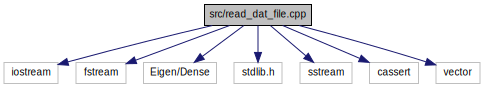
\includegraphics[width=350pt]{src_2read__dat__file_8cpp__incl}
\end{center}
\end{figure}
\subsection*{\-Functions}
\begin{DoxyCompactItemize}
\item 
double \hyperlink{src_2read__dat__file_8cpp_afe0bc81c124c80ed6a71504722cbecaf}{string\-\_\-to\-\_\-double} (string \&\hyperlink{get__klt__kernels_8m_a3691308f2a4c2f6983f2880d32e29c84}{s})
\item 
int \hyperlink{src_2read__dat__file_8cpp_a0ddf1224851353fc92bfbff6f499fa97}{main} (int argc, char $\ast$argv\mbox{[}$\,$\mbox{]})
\end{DoxyCompactItemize}


\subsection{\-Function \-Documentation}
\hypertarget{src_2read__dat__file_8cpp_a0ddf1224851353fc92bfbff6f499fa97}{\index{src/read\-\_\-dat\-\_\-file.\-cpp@{src/read\-\_\-dat\-\_\-file.\-cpp}!main@{main}}
\index{main@{main}!src/read_dat_file.cpp@{src/read\-\_\-dat\-\_\-file.\-cpp}}
\subsubsection[{main}]{\setlength{\rightskip}{0pt plus 5cm}int {\bf main} (
\begin{DoxyParamCaption}
\item[{int}]{argc, }
\item[{char $\ast$}]{argv\mbox{[}$\,$\mbox{]}}
\end{DoxyParamCaption}
)}}\label{src_2read__dat__file_8cpp_a0ddf1224851353fc92bfbff6f499fa97}


\-Here is the call graph for this function\-:
\nopagebreak
\begin{figure}[H]
\begin{center}
\leavevmode
\includegraphics[width=242pt]{src_2read__dat__file_8cpp_a0ddf1224851353fc92bfbff6f499fa97_cgraph}
\end{center}
\end{figure}


\hypertarget{src_2read__dat__file_8cpp_afe0bc81c124c80ed6a71504722cbecaf}{\index{src/read\-\_\-dat\-\_\-file.\-cpp@{src/read\-\_\-dat\-\_\-file.\-cpp}!string\-\_\-to\-\_\-double@{string\-\_\-to\-\_\-double}}
\index{string\-\_\-to\-\_\-double@{string\-\_\-to\-\_\-double}!src/read_dat_file.cpp@{src/read\-\_\-dat\-\_\-file.\-cpp}}
\subsubsection[{string\-\_\-to\-\_\-double}]{\setlength{\rightskip}{0pt plus 5cm}double {\bf string\-\_\-to\-\_\-double} (
\begin{DoxyParamCaption}
\item[{string \&}]{s}
\end{DoxyParamCaption}
)}}\label{src_2read__dat__file_8cpp_afe0bc81c124c80ed6a71504722cbecaf}

\input{gpu_2src_2save__params_8cpp}
\input{src_2save__params_8cpp}
\input{gpu_2src_2softmax__class_8cpp}
\input{src_2softmax__class_8cpp}
\hypertarget{gpu_2src_2test_8cpp}{\section{gpu/src/test.cpp \-File \-Reference}
\label{gpu_2src_2test_8cpp}\index{gpu/src/test.\-cpp@{gpu/src/test.\-cpp}}
}
{\ttfamily \#include \char`\"{}conv\-\_\-layer.\-h\char`\"{}}\*
{\ttfamily \#include \char`\"{}softmax\-\_\-class.\-h\char`\"{}}\*
{\ttfamily \#include $<$\-Eigen/\-Dense$>$}\*
{\ttfamily \#include $<$iostream$>$}\*
{\ttfamily \#include $<$vector$>$}\*
{\ttfamily \#include $<$cmath$>$}\*
{\ttfamily \#include $<$string$>$}\*
{\ttfamily \#include $<$ctime$>$}\*
\-Include dependency graph for test.\-cpp\-:
\nopagebreak
\begin{figure}[H]
\begin{center}
\leavevmode
\includegraphics[width=350pt]{gpu_2src_2test_8cpp__incl}
\end{center}
\end{figure}
\subsection*{\-Functions}
\begin{DoxyCompactItemize}
\item 
int \hyperlink{gpu_2src_2test_8cpp_ae66f6b31b5ad750f1fe042a706a4e3d4}{main} ()
\end{DoxyCompactItemize}


\subsection{\-Function \-Documentation}
\hypertarget{gpu_2src_2test_8cpp_ae66f6b31b5ad750f1fe042a706a4e3d4}{\index{gpu/src/test.\-cpp@{gpu/src/test.\-cpp}!main@{main}}
\index{main@{main}!gpu/src/test.cpp@{gpu/src/test.\-cpp}}
\subsubsection[{main}]{\setlength{\rightskip}{0pt plus 5cm}int {\bf main} (
\begin{DoxyParamCaption}
{}
\end{DoxyParamCaption}
)}}\label{gpu_2src_2test_8cpp_ae66f6b31b5ad750f1fe042a706a4e3d4}


\-Here is the call graph for this function\-:
\nopagebreak
\begin{figure}[H]
\begin{center}
\leavevmode
\includegraphics[width=320pt]{gpu_2src_2test_8cpp_ae66f6b31b5ad750f1fe042a706a4e3d4_cgraph}
\end{center}
\end{figure}



\hypertarget{src_2test_8cpp}{\section{src/test.cpp \-File \-Reference}
\label{src_2test_8cpp}\index{src/test.\-cpp@{src/test.\-cpp}}
}
{\ttfamily \#include \char`\"{}conv\-\_\-layer.\-h\char`\"{}}\*
{\ttfamily \#include \char`\"{}softmax\-\_\-class.\-h\char`\"{}}\*
{\ttfamily \#include $<$\-Eigen/\-Dense$>$}\*
{\ttfamily \#include $<$iostream$>$}\*
{\ttfamily \#include $<$vector$>$}\*
{\ttfamily \#include $<$cmath$>$}\*
{\ttfamily \#include $<$string$>$}\*
{\ttfamily \#include $<$ctime$>$}\*
\-Include dependency graph for test.\-cpp\-:
\nopagebreak
\begin{figure}[H]
\begin{center}
\leavevmode
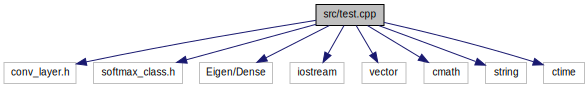
\includegraphics[width=350pt]{src_2test_8cpp__incl}
\end{center}
\end{figure}
\subsection*{\-Functions}
\begin{DoxyCompactItemize}
\item 
int \hyperlink{src_2test_8cpp_ae66f6b31b5ad750f1fe042a706a4e3d4}{main} ()
\end{DoxyCompactItemize}


\subsection{\-Function \-Documentation}
\hypertarget{src_2test_8cpp_ae66f6b31b5ad750f1fe042a706a4e3d4}{\index{src/test.\-cpp@{src/test.\-cpp}!main@{main}}
\index{main@{main}!src/test.cpp@{src/test.\-cpp}}
\subsubsection[{main}]{\setlength{\rightskip}{0pt plus 5cm}int {\bf main} (
\begin{DoxyParamCaption}
{}
\end{DoxyParamCaption}
)}}\label{src_2test_8cpp_ae66f6b31b5ad750f1fe042a706a4e3d4}


\-Here is the call graph for this function\-:
\nopagebreak
\begin{figure}[H]
\begin{center}
\leavevmode
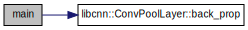
\includegraphics[width=320pt]{src_2test_8cpp_ae66f6b31b5ad750f1fe042a706a4e3d4_cgraph}
\end{center}
\end{figure}



\hypertarget{gpu_2src_2train_8cpp}{\section{gpu/src/train.cpp \-File \-Reference}
\label{gpu_2src_2train_8cpp}\index{gpu/src/train.\-cpp@{gpu/src/train.\-cpp}}
}
{\ttfamily \#include \char`\"{}conv\-\_\-layer.\-h\char`\"{}}\*
{\ttfamily \#include \char`\"{}softmax\-\_\-class.\-h\char`\"{}}\*
{\ttfamily \#include \char`\"{}pool.\-h\char`\"{}}\*
{\ttfamily \#include \char`\"{}load\-\_\-data.\-h\char`\"{}}\*
{\ttfamily \#include \char`\"{}init\-\_\-params.\-h\char`\"{}}\*
{\ttfamily \#include \char`\"{}preprocess.\-h\char`\"{}}\*
{\ttfamily \#include \char`\"{}rand\-\_\-initialize.\-h\char`\"{}}\*
{\ttfamily \#include $<$\-Eigen/\-Dense$>$}\*
{\ttfamily \#include $<$iostream$>$}\*
{\ttfamily \#include $<$vector$>$}\*
{\ttfamily \#include $<$cmath$>$}\*
{\ttfamily \#include $<$string$>$}\*
{\ttfamily \#include $<$ctime$>$}\*
{\ttfamily \#include $<$sys/types.\-h$>$}\*
{\ttfamily \#include $<$dirent.\-h$>$}\*
{\ttfamily \#include $<$cstdlib$>$}\*
{\ttfamily \#include $<$cassert$>$}\*
{\ttfamily \#include $<$algorithm$>$}\*
{\ttfamily \#include $<$stdio.\-h$>$}\*
{\ttfamily \#include \char`\"{}yaml-\/cpp/yaml.\-h\char`\"{}}\*
\-Include dependency graph for train.\-cpp\-:
\nopagebreak
\begin{figure}[H]
\begin{center}
\leavevmode
\includegraphics[width=350pt]{gpu_2src_2train_8cpp__incl}
\end{center}
\end{figure}
\subsection*{\-Defines}
\begin{DoxyCompactItemize}
\item 
\#define \hyperlink{gpu_2src_2train_8cpp_a34b04bd23b07b485921a728ad0805ac4}{\-M\-A\-I\-N}
\item 
\#define \hyperlink{gpu_2src_2train_8cpp_ab2868d85c8a74e3ee08bdc44580e2235}{\-S\-A\-V\-E}
\end{DoxyCompactItemize}
\subsection*{\-Functions}
\begin{DoxyCompactItemize}
\item 
void \hyperlink{gpu_2src_2train_8cpp_a7bc382c1af51bbe0abf0f61a5e98c99c}{print\-\_\-conv} (const vector$<$ \-Matrix\-Xd $>$ \&weights, const \-Matrix\-Xd \&biases)
\item 
void \hyperlink{gpu_2src_2train_8cpp_a8d8f47ed70e9d49f1a0361ee478ee55b}{print\-\_\-class} (const \-Matrix\-Xd \&weight, const \-Matrix\-Xd \&bias)
\item 
void \hyperlink{gpu_2src_2train_8cpp_a6113682517703008d4dea0c653448610}{training\-\_\-single} ()
\item 
void \hyperlink{gpu_2src_2train_8cpp_a85d8021bce07b2466383f3891dc6c913}{training\-\_\-batch} ()
\item 
int \hyperlink{gpu_2src_2train_8cpp_ae66f6b31b5ad750f1fe042a706a4e3d4}{main} ()
\end{DoxyCompactItemize}
\subsection*{\-Variables}
\begin{DoxyCompactItemize}
\item 
const int \hyperlink{gpu_2src_2train_8cpp_a8476ec27c8e5400b7eec34f0d0ad6be6}{image\-\_\-height} = 320
\item 
const int \hyperlink{gpu_2src_2train_8cpp_a864b445a94b3a4416c82a97ab9cd3a55}{image\-\_\-width} = 240
\item 
const int \hyperlink{gpu_2src_2train_8cpp_af17a6f9c9fc8fc26d1645cf6291bb0d9}{pool} = 8
\item 
const int \hyperlink{gpu_2src_2train_8cpp_a9b2018494ed2bdca5175de5bea19b198}{num\-\_\-kerns1} = 4
\item 
const int \hyperlink{gpu_2src_2train_8cpp_a5b047b4d1dd331bbb11859d5b91c9f8f}{num\-\_\-kerns2} = 6
\item 
const int \hyperlink{gpu_2src_2train_8cpp_a0b12f9b542065fa65cb8604002c2799d}{num\-\_\-kerns3} = 8
\item 
const int \hyperlink{gpu_2src_2train_8cpp_a39899a59e72620ab32d676987dd8ba49}{kernel\-\_\-size} = 7
\item 
const int \hyperlink{gpu_2src_2train_8cpp_a8917e12c91d83995f62f81e68aa9cb6b}{num\-\_\-labels} = 9
\item 
const double \hyperlink{gpu_2src_2train_8cpp_aa1b0a484ac95c8aa6e11ff885a2dae78}{weight\-\_\-bound} = 0.\-1
\item 
const double \hyperlink{gpu_2src_2train_8cpp_a032a7a5229c6fd6a22f96436ae9500fa}{bias\-\_\-bound} = 0.\-01
\item 
const double \hyperlink{gpu_2src_2train_8cpp_a92f3087835c14040e65651f0638ca507}{wb} = 0.\-05
\item 
const double \hyperlink{gpu_2src_2train_8cpp_a91f56d5c28de4346a57200665d995784}{bb} = 0.\-0005
\item 
const int \hyperlink{gpu_2src_2train_8cpp_aeda9aa6239a9e3337b85ef51668739d3}{num\-\_\-input\-\_\-channels} = 3
\item 
const int \hyperlink{gpu_2src_2train_8cpp_ac8d3682725de2f401975e90712ce1e5c}{pool\-\_\-size} = 2
\item 
double \hyperlink{gpu_2src_2train_8cpp_abaa236ecd5f1965a51e3e3337e1a4ae5}{learning\-\_\-rate1} = 0.\-01
\item 
double \hyperlink{gpu_2src_2train_8cpp_af91776424ae6645e9b60e25640c418ed}{learning\-\_\-rate2} = 0.\-01
\item 
const int \hyperlink{gpu_2src_2train_8cpp_a326e252cb0b0ed7a7b634b0cfab52a28}{num\-\_\-images} = 200
\item 
const int \hyperlink{gpu_2src_2train_8cpp_a2c643af60711df9339a5a9fb6519148b}{batch\-\_\-size} = 40
\item 
const int \hyperlink{gpu_2src_2train_8cpp_ab11165448f7def007498acd8283a10ff}{num\-\_\-batches} = \hyperlink{validate_8cpp_a326e252cb0b0ed7a7b634b0cfab52a28}{num\-\_\-images} / \hyperlink{src_2train_8cpp_a2c643af60711df9339a5a9fb6519148b}{batch\-\_\-size}
\item 
int \hyperlink{gpu_2src_2train_8cpp_a34f4541b93687f4eba94f12aadd95050}{beginning} = 1
\item 
const int \hyperlink{gpu_2src_2train_8cpp_a76ec1a7087432a2317f948b84b6bd788}{loop} = 500
\end{DoxyCompactItemize}


\subsection{\-Define \-Documentation}
\hypertarget{gpu_2src_2train_8cpp_a34b04bd23b07b485921a728ad0805ac4}{\index{gpu/src/train.\-cpp@{gpu/src/train.\-cpp}!\-M\-A\-I\-N@{\-M\-A\-I\-N}}
\index{\-M\-A\-I\-N@{\-M\-A\-I\-N}!gpu/src/train.cpp@{gpu/src/train.\-cpp}}
\subsubsection[{\-M\-A\-I\-N}]{\setlength{\rightskip}{0pt plus 5cm}\#define {\bf \-M\-A\-I\-N}}}\label{gpu_2src_2train_8cpp_a34b04bd23b07b485921a728ad0805ac4}
\hypertarget{gpu_2src_2train_8cpp_ab2868d85c8a74e3ee08bdc44580e2235}{\index{gpu/src/train.\-cpp@{gpu/src/train.\-cpp}!\-S\-A\-V\-E@{\-S\-A\-V\-E}}
\index{\-S\-A\-V\-E@{\-S\-A\-V\-E}!gpu/src/train.cpp@{gpu/src/train.\-cpp}}
\subsubsection[{\-S\-A\-V\-E}]{\setlength{\rightskip}{0pt plus 5cm}\#define {\bf \-S\-A\-V\-E}}}\label{gpu_2src_2train_8cpp_ab2868d85c8a74e3ee08bdc44580e2235}


\subsection{\-Function \-Documentation}
\hypertarget{gpu_2src_2train_8cpp_ae66f6b31b5ad750f1fe042a706a4e3d4}{\index{gpu/src/train.\-cpp@{gpu/src/train.\-cpp}!main@{main}}
\index{main@{main}!gpu/src/train.cpp@{gpu/src/train.\-cpp}}
\subsubsection[{main}]{\setlength{\rightskip}{0pt plus 5cm}int {\bf main} (
\begin{DoxyParamCaption}
{}
\end{DoxyParamCaption}
)}}\label{gpu_2src_2train_8cpp_ae66f6b31b5ad750f1fe042a706a4e3d4}


\-Here is the call graph for this function\-:
\nopagebreak
\begin{figure}[H]
\begin{center}
\leavevmode
\includegraphics[width=350pt]{gpu_2src_2train_8cpp_ae66f6b31b5ad750f1fe042a706a4e3d4_cgraph}
\end{center}
\end{figure}


\hypertarget{gpu_2src_2train_8cpp_a8d8f47ed70e9d49f1a0361ee478ee55b}{\index{gpu/src/train.\-cpp@{gpu/src/train.\-cpp}!print\-\_\-class@{print\-\_\-class}}
\index{print\-\_\-class@{print\-\_\-class}!gpu/src/train.cpp@{gpu/src/train.\-cpp}}
\subsubsection[{print\-\_\-class}]{\setlength{\rightskip}{0pt plus 5cm}void {\bf print\-\_\-class} (
\begin{DoxyParamCaption}
\item[{const \-Matrix\-Xd \&}]{weight, }
\item[{const \-Matrix\-Xd \&}]{bias}
\end{DoxyParamCaption}
)}}\label{gpu_2src_2train_8cpp_a8d8f47ed70e9d49f1a0361ee478ee55b}
\hypertarget{gpu_2src_2train_8cpp_a7bc382c1af51bbe0abf0f61a5e98c99c}{\index{gpu/src/train.\-cpp@{gpu/src/train.\-cpp}!print\-\_\-conv@{print\-\_\-conv}}
\index{print\-\_\-conv@{print\-\_\-conv}!gpu/src/train.cpp@{gpu/src/train.\-cpp}}
\subsubsection[{print\-\_\-conv}]{\setlength{\rightskip}{0pt plus 5cm}void {\bf print\-\_\-conv} (
\begin{DoxyParamCaption}
\item[{const vector$<$ \-Matrix\-Xd $>$ \&}]{weights, }
\item[{const \-Matrix\-Xd \&}]{biases}
\end{DoxyParamCaption}
)}}\label{gpu_2src_2train_8cpp_a7bc382c1af51bbe0abf0f61a5e98c99c}
\hypertarget{gpu_2src_2train_8cpp_a85d8021bce07b2466383f3891dc6c913}{\index{gpu/src/train.\-cpp@{gpu/src/train.\-cpp}!training\-\_\-batch@{training\-\_\-batch}}
\index{training\-\_\-batch@{training\-\_\-batch}!gpu/src/train.cpp@{gpu/src/train.\-cpp}}
\subsubsection[{training\-\_\-batch}]{\setlength{\rightskip}{0pt plus 5cm}void {\bf training\-\_\-batch} (
\begin{DoxyParamCaption}
{}
\end{DoxyParamCaption}
)}}\label{gpu_2src_2train_8cpp_a85d8021bce07b2466383f3891dc6c913}


\-Here is the call graph for this function\-:
\nopagebreak
\begin{figure}[H]
\begin{center}
\leavevmode
\includegraphics[width=350pt]{gpu_2src_2train_8cpp_a85d8021bce07b2466383f3891dc6c913_cgraph}
\end{center}
\end{figure}


\hypertarget{gpu_2src_2train_8cpp_a6113682517703008d4dea0c653448610}{\index{gpu/src/train.\-cpp@{gpu/src/train.\-cpp}!training\-\_\-single@{training\-\_\-single}}
\index{training\-\_\-single@{training\-\_\-single}!gpu/src/train.cpp@{gpu/src/train.\-cpp}}
\subsubsection[{training\-\_\-single}]{\setlength{\rightskip}{0pt plus 5cm}void {\bf training\-\_\-single} (
\begin{DoxyParamCaption}
{}
\end{DoxyParamCaption}
)}}\label{gpu_2src_2train_8cpp_a6113682517703008d4dea0c653448610}


\-Here is the call graph for this function\-:
\nopagebreak
\begin{figure}[H]
\begin{center}
\leavevmode
\includegraphics[width=350pt]{gpu_2src_2train_8cpp_a6113682517703008d4dea0c653448610_cgraph}
\end{center}
\end{figure}




\subsection{\-Variable \-Documentation}
\hypertarget{gpu_2src_2train_8cpp_a2c643af60711df9339a5a9fb6519148b}{\index{gpu/src/train.\-cpp@{gpu/src/train.\-cpp}!batch\-\_\-size@{batch\-\_\-size}}
\index{batch\-\_\-size@{batch\-\_\-size}!gpu/src/train.cpp@{gpu/src/train.\-cpp}}
\subsubsection[{batch\-\_\-size}]{\setlength{\rightskip}{0pt plus 5cm}const int {\bf batch\-\_\-size} = 40}}\label{gpu_2src_2train_8cpp_a2c643af60711df9339a5a9fb6519148b}
\hypertarget{gpu_2src_2train_8cpp_a91f56d5c28de4346a57200665d995784}{\index{gpu/src/train.\-cpp@{gpu/src/train.\-cpp}!bb@{bb}}
\index{bb@{bb}!gpu/src/train.cpp@{gpu/src/train.\-cpp}}
\subsubsection[{bb}]{\setlength{\rightskip}{0pt plus 5cm}const double {\bf bb} = 0.\-0005}}\label{gpu_2src_2train_8cpp_a91f56d5c28de4346a57200665d995784}
\hypertarget{gpu_2src_2train_8cpp_a34f4541b93687f4eba94f12aadd95050}{\index{gpu/src/train.\-cpp@{gpu/src/train.\-cpp}!beginning@{beginning}}
\index{beginning@{beginning}!gpu/src/train.cpp@{gpu/src/train.\-cpp}}
\subsubsection[{beginning}]{\setlength{\rightskip}{0pt plus 5cm}int {\bf beginning} = 1}}\label{gpu_2src_2train_8cpp_a34f4541b93687f4eba94f12aadd95050}
\hypertarget{gpu_2src_2train_8cpp_a032a7a5229c6fd6a22f96436ae9500fa}{\index{gpu/src/train.\-cpp@{gpu/src/train.\-cpp}!bias\-\_\-bound@{bias\-\_\-bound}}
\index{bias\-\_\-bound@{bias\-\_\-bound}!gpu/src/train.cpp@{gpu/src/train.\-cpp}}
\subsubsection[{bias\-\_\-bound}]{\setlength{\rightskip}{0pt plus 5cm}const double {\bf bias\-\_\-bound} = 0.\-01}}\label{gpu_2src_2train_8cpp_a032a7a5229c6fd6a22f96436ae9500fa}
\hypertarget{gpu_2src_2train_8cpp_a8476ec27c8e5400b7eec34f0d0ad6be6}{\index{gpu/src/train.\-cpp@{gpu/src/train.\-cpp}!image\-\_\-height@{image\-\_\-height}}
\index{image\-\_\-height@{image\-\_\-height}!gpu/src/train.cpp@{gpu/src/train.\-cpp}}
\subsubsection[{image\-\_\-height}]{\setlength{\rightskip}{0pt plus 5cm}const int {\bf image\-\_\-height} = 320}}\label{gpu_2src_2train_8cpp_a8476ec27c8e5400b7eec34f0d0ad6be6}
\hypertarget{gpu_2src_2train_8cpp_a864b445a94b3a4416c82a97ab9cd3a55}{\index{gpu/src/train.\-cpp@{gpu/src/train.\-cpp}!image\-\_\-width@{image\-\_\-width}}
\index{image\-\_\-width@{image\-\_\-width}!gpu/src/train.cpp@{gpu/src/train.\-cpp}}
\subsubsection[{image\-\_\-width}]{\setlength{\rightskip}{0pt plus 5cm}const int {\bf image\-\_\-width} = 240}}\label{gpu_2src_2train_8cpp_a864b445a94b3a4416c82a97ab9cd3a55}
\hypertarget{gpu_2src_2train_8cpp_a39899a59e72620ab32d676987dd8ba49}{\index{gpu/src/train.\-cpp@{gpu/src/train.\-cpp}!kernel\-\_\-size@{kernel\-\_\-size}}
\index{kernel\-\_\-size@{kernel\-\_\-size}!gpu/src/train.cpp@{gpu/src/train.\-cpp}}
\subsubsection[{kernel\-\_\-size}]{\setlength{\rightskip}{0pt plus 5cm}const int {\bf kernel\-\_\-size} = 7}}\label{gpu_2src_2train_8cpp_a39899a59e72620ab32d676987dd8ba49}
\hypertarget{gpu_2src_2train_8cpp_abaa236ecd5f1965a51e3e3337e1a4ae5}{\index{gpu/src/train.\-cpp@{gpu/src/train.\-cpp}!learning\-\_\-rate1@{learning\-\_\-rate1}}
\index{learning\-\_\-rate1@{learning\-\_\-rate1}!gpu/src/train.cpp@{gpu/src/train.\-cpp}}
\subsubsection[{learning\-\_\-rate1}]{\setlength{\rightskip}{0pt plus 5cm}double {\bf learning\-\_\-rate1} = 0.\-01}}\label{gpu_2src_2train_8cpp_abaa236ecd5f1965a51e3e3337e1a4ae5}
\hypertarget{gpu_2src_2train_8cpp_af91776424ae6645e9b60e25640c418ed}{\index{gpu/src/train.\-cpp@{gpu/src/train.\-cpp}!learning\-\_\-rate2@{learning\-\_\-rate2}}
\index{learning\-\_\-rate2@{learning\-\_\-rate2}!gpu/src/train.cpp@{gpu/src/train.\-cpp}}
\subsubsection[{learning\-\_\-rate2}]{\setlength{\rightskip}{0pt plus 5cm}double {\bf learning\-\_\-rate2} = 0.\-01}}\label{gpu_2src_2train_8cpp_af91776424ae6645e9b60e25640c418ed}
\hypertarget{gpu_2src_2train_8cpp_a76ec1a7087432a2317f948b84b6bd788}{\index{gpu/src/train.\-cpp@{gpu/src/train.\-cpp}!loop@{loop}}
\index{loop@{loop}!gpu/src/train.cpp@{gpu/src/train.\-cpp}}
\subsubsection[{loop}]{\setlength{\rightskip}{0pt plus 5cm}const int {\bf loop} = 500}}\label{gpu_2src_2train_8cpp_a76ec1a7087432a2317f948b84b6bd788}
\hypertarget{gpu_2src_2train_8cpp_ab11165448f7def007498acd8283a10ff}{\index{gpu/src/train.\-cpp@{gpu/src/train.\-cpp}!num\-\_\-batches@{num\-\_\-batches}}
\index{num\-\_\-batches@{num\-\_\-batches}!gpu/src/train.cpp@{gpu/src/train.\-cpp}}
\subsubsection[{num\-\_\-batches}]{\setlength{\rightskip}{0pt plus 5cm}const int {\bf num\-\_\-batches} = {\bf num\-\_\-images} / {\bf batch\-\_\-size}}}\label{gpu_2src_2train_8cpp_ab11165448f7def007498acd8283a10ff}
\hypertarget{gpu_2src_2train_8cpp_a326e252cb0b0ed7a7b634b0cfab52a28}{\index{gpu/src/train.\-cpp@{gpu/src/train.\-cpp}!num\-\_\-images@{num\-\_\-images}}
\index{num\-\_\-images@{num\-\_\-images}!gpu/src/train.cpp@{gpu/src/train.\-cpp}}
\subsubsection[{num\-\_\-images}]{\setlength{\rightskip}{0pt plus 5cm}const int {\bf num\-\_\-images} = 200}}\label{gpu_2src_2train_8cpp_a326e252cb0b0ed7a7b634b0cfab52a28}
\hypertarget{gpu_2src_2train_8cpp_aeda9aa6239a9e3337b85ef51668739d3}{\index{gpu/src/train.\-cpp@{gpu/src/train.\-cpp}!num\-\_\-input\-\_\-channels@{num\-\_\-input\-\_\-channels}}
\index{num\-\_\-input\-\_\-channels@{num\-\_\-input\-\_\-channels}!gpu/src/train.cpp@{gpu/src/train.\-cpp}}
\subsubsection[{num\-\_\-input\-\_\-channels}]{\setlength{\rightskip}{0pt plus 5cm}const int {\bf num\-\_\-input\-\_\-channels} = 3}}\label{gpu_2src_2train_8cpp_aeda9aa6239a9e3337b85ef51668739d3}
\hypertarget{gpu_2src_2train_8cpp_a9b2018494ed2bdca5175de5bea19b198}{\index{gpu/src/train.\-cpp@{gpu/src/train.\-cpp}!num\-\_\-kerns1@{num\-\_\-kerns1}}
\index{num\-\_\-kerns1@{num\-\_\-kerns1}!gpu/src/train.cpp@{gpu/src/train.\-cpp}}
\subsubsection[{num\-\_\-kerns1}]{\setlength{\rightskip}{0pt plus 5cm}const int {\bf num\-\_\-kerns1} = 4}}\label{gpu_2src_2train_8cpp_a9b2018494ed2bdca5175de5bea19b198}
\hypertarget{gpu_2src_2train_8cpp_a5b047b4d1dd331bbb11859d5b91c9f8f}{\index{gpu/src/train.\-cpp@{gpu/src/train.\-cpp}!num\-\_\-kerns2@{num\-\_\-kerns2}}
\index{num\-\_\-kerns2@{num\-\_\-kerns2}!gpu/src/train.cpp@{gpu/src/train.\-cpp}}
\subsubsection[{num\-\_\-kerns2}]{\setlength{\rightskip}{0pt plus 5cm}const int {\bf num\-\_\-kerns2} = 6}}\label{gpu_2src_2train_8cpp_a5b047b4d1dd331bbb11859d5b91c9f8f}
\hypertarget{gpu_2src_2train_8cpp_a0b12f9b542065fa65cb8604002c2799d}{\index{gpu/src/train.\-cpp@{gpu/src/train.\-cpp}!num\-\_\-kerns3@{num\-\_\-kerns3}}
\index{num\-\_\-kerns3@{num\-\_\-kerns3}!gpu/src/train.cpp@{gpu/src/train.\-cpp}}
\subsubsection[{num\-\_\-kerns3}]{\setlength{\rightskip}{0pt plus 5cm}const int {\bf num\-\_\-kerns3} = 8}}\label{gpu_2src_2train_8cpp_a0b12f9b542065fa65cb8604002c2799d}
\hypertarget{gpu_2src_2train_8cpp_a8917e12c91d83995f62f81e68aa9cb6b}{\index{gpu/src/train.\-cpp@{gpu/src/train.\-cpp}!num\-\_\-labels@{num\-\_\-labels}}
\index{num\-\_\-labels@{num\-\_\-labels}!gpu/src/train.cpp@{gpu/src/train.\-cpp}}
\subsubsection[{num\-\_\-labels}]{\setlength{\rightskip}{0pt plus 5cm}const int {\bf num\-\_\-labels} = 9}}\label{gpu_2src_2train_8cpp_a8917e12c91d83995f62f81e68aa9cb6b}
\hypertarget{gpu_2src_2train_8cpp_af17a6f9c9fc8fc26d1645cf6291bb0d9}{\index{gpu/src/train.\-cpp@{gpu/src/train.\-cpp}!pool@{pool}}
\index{pool@{pool}!gpu/src/train.cpp@{gpu/src/train.\-cpp}}
\subsubsection[{pool}]{\setlength{\rightskip}{0pt plus 5cm}const int {\bf pool} = 8}}\label{gpu_2src_2train_8cpp_af17a6f9c9fc8fc26d1645cf6291bb0d9}
\hypertarget{gpu_2src_2train_8cpp_ac8d3682725de2f401975e90712ce1e5c}{\index{gpu/src/train.\-cpp@{gpu/src/train.\-cpp}!pool\-\_\-size@{pool\-\_\-size}}
\index{pool\-\_\-size@{pool\-\_\-size}!gpu/src/train.cpp@{gpu/src/train.\-cpp}}
\subsubsection[{pool\-\_\-size}]{\setlength{\rightskip}{0pt plus 5cm}const int {\bf pool\-\_\-size} = 2}}\label{gpu_2src_2train_8cpp_ac8d3682725de2f401975e90712ce1e5c}
\hypertarget{gpu_2src_2train_8cpp_a92f3087835c14040e65651f0638ca507}{\index{gpu/src/train.\-cpp@{gpu/src/train.\-cpp}!wb@{wb}}
\index{wb@{wb}!gpu/src/train.cpp@{gpu/src/train.\-cpp}}
\subsubsection[{wb}]{\setlength{\rightskip}{0pt plus 5cm}const double {\bf wb} = 0.\-05}}\label{gpu_2src_2train_8cpp_a92f3087835c14040e65651f0638ca507}
\hypertarget{gpu_2src_2train_8cpp_aa1b0a484ac95c8aa6e11ff885a2dae78}{\index{gpu/src/train.\-cpp@{gpu/src/train.\-cpp}!weight\-\_\-bound@{weight\-\_\-bound}}
\index{weight\-\_\-bound@{weight\-\_\-bound}!gpu/src/train.cpp@{gpu/src/train.\-cpp}}
\subsubsection[{weight\-\_\-bound}]{\setlength{\rightskip}{0pt plus 5cm}const double {\bf weight\-\_\-bound} = 0.\-1}}\label{gpu_2src_2train_8cpp_aa1b0a484ac95c8aa6e11ff885a2dae78}

\input{src_2train_8cpp}
\hypertarget{gtest__softmax_8cpp}{\section{gtest\-\_\-softmax.\-cpp \-File \-Reference}
\label{gtest__softmax_8cpp}\index{gtest\-\_\-softmax.\-cpp@{gtest\-\_\-softmax.\-cpp}}
}
{\ttfamily \#include $<$\-Eigen/\-Dense$>$}\*
{\ttfamily \#include $<$math.\-h$>$}\*
{\ttfamily \#include $<$stdlib.\-h$>$}\*
{\ttfamily \#include $<$iostream$>$}\*
{\ttfamily \#include $<$gtest/gtest.\-h$>$}\*
{\ttfamily \#include $<$fstream$>$}\*
{\ttfamily \#include \char`\"{}yaml-\/cpp/yaml.\-h\char`\"{}}\*
{\ttfamily \#include $<$string$>$}\*
{\ttfamily \#include $<$string.\-h$>$}\*
{\ttfamily \#include \char`\"{}softmax\-\_\-class.\-cpp\char`\"{}}\*
\-Include dependency graph for gtest\-\_\-softmax.\-cpp\-:
\nopagebreak
\begin{figure}[H]
\begin{center}
\leavevmode
\includegraphics[width=350pt]{gtest__softmax_8cpp__incl}
\end{center}
\end{figure}
\subsection*{\-Functions}
\begin{DoxyCompactItemize}
\item 
\-Matrix\-Xd \hyperlink{gtest__softmax_8cpp_ab7d7b4f078e317d92400b9bb0b9bdb86}{cnn\-\_\-output} (3, 3)
\item 
\-Vector\-Xi \hyperlink{gtest__softmax_8cpp_ab74d1bf93fd1d95503a8200069ae04c0}{ground\-\_\-truth} (3)
\item 
void \hyperlink{gtest__softmax_8cpp_a15e6c82d14b7cde034d53e566fd2ff8e}{parser\-\_\-yaml\-\_\-para} (string \&\hyperlink{yaml__t__load_8cpp_a7f01c047eb310166e695d4232ebd1fae}{dir}, \-Matrix\-Xd \&\hyperlink{yaml__t__load_8cpp_a600eac78667d5a813045d8ef2f4395dd}{d}, int \&\hyperlink{yaml__t__load_8cpp_a62c66ce2f11b397011ce5d92cc33f6c0}{\-Label\-\_\-number}, \-Vector\-Xi \&\hyperlink{yaml__t__load_8cpp_a80d599bd22867a8e610e0be09bf1128d}{v}, double \&\hyperlink{yaml__t__load_8cpp_acb484cd30430928d888abe1cfda0d9bb}{w\-\_\-bound}, double \&\hyperlink{yaml__t__load_8cpp_a674b759c775a81169ae20a20b4b2f4db}{b\-\_\-bound}, double \&\hyperlink{yaml__t__load_8cpp_a7b45f711c59e30b2aa59c4c954ad8ea1}{learning\-\_\-rate})
\item 
\hyperlink{gtest__softmax_8cpp_a7000779f1149fa088f0c83972dfcbb8b}{\-T\-E\-S\-T} (\-Int\-Test, \-Int\-Number)
\item 
int \hyperlink{gtest__softmax_8cpp_a0ddf1224851353fc92bfbff6f499fa97}{main} (int argc, char $\ast$argv\mbox{[}$\,$\mbox{]})
\end{DoxyCompactItemize}
\subsection*{\-Variables}
\begin{DoxyCompactItemize}
\item 
string \hyperlink{gtest__softmax_8cpp_a7f01c047eb310166e695d4232ebd1fae}{dir} = string (\char`\"{}../seq.\-yaml\char`\"{})
\item 
int \hyperlink{gtest__softmax_8cpp_a62c66ce2f11b397011ce5d92cc33f6c0}{\-Label\-\_\-number}
\item 
double \hyperlink{gtest__softmax_8cpp_acb484cd30430928d888abe1cfda0d9bb}{w\-\_\-bound}
\item 
double \hyperlink{gtest__softmax_8cpp_a674b759c775a81169ae20a20b4b2f4db}{b\-\_\-bound}
\item 
double \hyperlink{gtest__softmax_8cpp_a7b45f711c59e30b2aa59c4c954ad8ea1}{learning\-\_\-rate}
\end{DoxyCompactItemize}


\subsection{\-Function \-Documentation}
\hypertarget{gtest__softmax_8cpp_ab7d7b4f078e317d92400b9bb0b9bdb86}{\index{gtest\-\_\-softmax.\-cpp@{gtest\-\_\-softmax.\-cpp}!cnn\-\_\-output@{cnn\-\_\-output}}
\index{cnn\-\_\-output@{cnn\-\_\-output}!gtest_softmax.cpp@{gtest\-\_\-softmax.\-cpp}}
\subsubsection[{cnn\-\_\-output}]{\setlength{\rightskip}{0pt plus 5cm}\-Matrix\-Xd {\bf cnn\-\_\-output} (
\begin{DoxyParamCaption}
\item[{3}]{, }
\item[{3}]{}
\end{DoxyParamCaption}
)}}\label{gtest__softmax_8cpp_ab7d7b4f078e317d92400b9bb0b9bdb86}
\hypertarget{gtest__softmax_8cpp_ab74d1bf93fd1d95503a8200069ae04c0}{\index{gtest\-\_\-softmax.\-cpp@{gtest\-\_\-softmax.\-cpp}!ground\-\_\-truth@{ground\-\_\-truth}}
\index{ground\-\_\-truth@{ground\-\_\-truth}!gtest_softmax.cpp@{gtest\-\_\-softmax.\-cpp}}
\subsubsection[{ground\-\_\-truth}]{\setlength{\rightskip}{0pt plus 5cm}\-Vector\-Xi {\bf ground\-\_\-truth} (
\begin{DoxyParamCaption}
\item[{3}]{}
\end{DoxyParamCaption}
)}}\label{gtest__softmax_8cpp_ab74d1bf93fd1d95503a8200069ae04c0}
\hypertarget{gtest__softmax_8cpp_a0ddf1224851353fc92bfbff6f499fa97}{\index{gtest\-\_\-softmax.\-cpp@{gtest\-\_\-softmax.\-cpp}!main@{main}}
\index{main@{main}!gtest_softmax.cpp@{gtest\-\_\-softmax.\-cpp}}
\subsubsection[{main}]{\setlength{\rightskip}{0pt plus 5cm}int {\bf main} (
\begin{DoxyParamCaption}
\item[{int}]{argc, }
\item[{char $\ast$}]{argv\mbox{[}$\,$\mbox{]}}
\end{DoxyParamCaption}
)}}\label{gtest__softmax_8cpp_a0ddf1224851353fc92bfbff6f499fa97}
\hypertarget{gtest__softmax_8cpp_a15e6c82d14b7cde034d53e566fd2ff8e}{\index{gtest\-\_\-softmax.\-cpp@{gtest\-\_\-softmax.\-cpp}!parser\-\_\-yaml\-\_\-para@{parser\-\_\-yaml\-\_\-para}}
\index{parser\-\_\-yaml\-\_\-para@{parser\-\_\-yaml\-\_\-para}!gtest_softmax.cpp@{gtest\-\_\-softmax.\-cpp}}
\subsubsection[{parser\-\_\-yaml\-\_\-para}]{\setlength{\rightskip}{0pt plus 5cm}void {\bf parser\-\_\-yaml\-\_\-para} (
\begin{DoxyParamCaption}
\item[{string \&}]{dir, }
\item[{\-Matrix\-Xd \&}]{d, }
\item[{int \&}]{\-Label\-\_\-number, }
\item[{\-Vector\-Xi \&}]{v, }
\item[{double \&}]{w\-\_\-bound, }
\item[{double \&}]{b\-\_\-bound, }
\item[{double \&}]{learning\-\_\-rate}
\end{DoxyParamCaption}
)}}\label{gtest__softmax_8cpp_a15e6c82d14b7cde034d53e566fd2ff8e}


\-Here is the call graph for this function\-:
\nopagebreak
\begin{figure}[H]
\begin{center}
\leavevmode
\includegraphics[width=240pt]{gtest__softmax_8cpp_a15e6c82d14b7cde034d53e566fd2ff8e_cgraph}
\end{center}
\end{figure}


\hypertarget{gtest__softmax_8cpp_a7000779f1149fa088f0c83972dfcbb8b}{\index{gtest\-\_\-softmax.\-cpp@{gtest\-\_\-softmax.\-cpp}!\-T\-E\-S\-T@{\-T\-E\-S\-T}}
\index{\-T\-E\-S\-T@{\-T\-E\-S\-T}!gtest_softmax.cpp@{gtest\-\_\-softmax.\-cpp}}
\subsubsection[{\-T\-E\-S\-T}]{\setlength{\rightskip}{0pt plus 5cm}{\bf \-T\-E\-S\-T} (
\begin{DoxyParamCaption}
\item[{\-Int\-Test}]{, }
\item[{\-Int\-Number}]{}
\end{DoxyParamCaption}
)}}\label{gtest__softmax_8cpp_a7000779f1149fa088f0c83972dfcbb8b}


\-Here is the call graph for this function\-:
\nopagebreak
\begin{figure}[H]
\begin{center}
\leavevmode
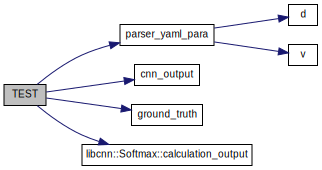
\includegraphics[width=350pt]{gtest__softmax_8cpp_a7000779f1149fa088f0c83972dfcbb8b_cgraph}
\end{center}
\end{figure}




\subsection{\-Variable \-Documentation}
\hypertarget{gtest__softmax_8cpp_a674b759c775a81169ae20a20b4b2f4db}{\index{gtest\-\_\-softmax.\-cpp@{gtest\-\_\-softmax.\-cpp}!b\-\_\-bound@{b\-\_\-bound}}
\index{b\-\_\-bound@{b\-\_\-bound}!gtest_softmax.cpp@{gtest\-\_\-softmax.\-cpp}}
\subsubsection[{b\-\_\-bound}]{\setlength{\rightskip}{0pt plus 5cm}double {\bf b\-\_\-bound}}}\label{gtest__softmax_8cpp_a674b759c775a81169ae20a20b4b2f4db}
\hypertarget{gtest__softmax_8cpp_a7f01c047eb310166e695d4232ebd1fae}{\index{gtest\-\_\-softmax.\-cpp@{gtest\-\_\-softmax.\-cpp}!dir@{dir}}
\index{dir@{dir}!gtest_softmax.cpp@{gtest\-\_\-softmax.\-cpp}}
\subsubsection[{dir}]{\setlength{\rightskip}{0pt plus 5cm}string {\bf dir} = string (\char`\"{}../seq.\-yaml\char`\"{})}}\label{gtest__softmax_8cpp_a7f01c047eb310166e695d4232ebd1fae}
\hypertarget{gtest__softmax_8cpp_a62c66ce2f11b397011ce5d92cc33f6c0}{\index{gtest\-\_\-softmax.\-cpp@{gtest\-\_\-softmax.\-cpp}!\-Label\-\_\-number@{\-Label\-\_\-number}}
\index{\-Label\-\_\-number@{\-Label\-\_\-number}!gtest_softmax.cpp@{gtest\-\_\-softmax.\-cpp}}
\subsubsection[{\-Label\-\_\-number}]{\setlength{\rightskip}{0pt plus 5cm}int {\bf \-Label\-\_\-number}}}\label{gtest__softmax_8cpp_a62c66ce2f11b397011ce5d92cc33f6c0}
\hypertarget{gtest__softmax_8cpp_a7b45f711c59e30b2aa59c4c954ad8ea1}{\index{gtest\-\_\-softmax.\-cpp@{gtest\-\_\-softmax.\-cpp}!learning\-\_\-rate@{learning\-\_\-rate}}
\index{learning\-\_\-rate@{learning\-\_\-rate}!gtest_softmax.cpp@{gtest\-\_\-softmax.\-cpp}}
\subsubsection[{learning\-\_\-rate}]{\setlength{\rightskip}{0pt plus 5cm}double {\bf learning\-\_\-rate}}}\label{gtest__softmax_8cpp_a7b45f711c59e30b2aa59c4c954ad8ea1}
\hypertarget{gtest__softmax_8cpp_acb484cd30430928d888abe1cfda0d9bb}{\index{gtest\-\_\-softmax.\-cpp@{gtest\-\_\-softmax.\-cpp}!w\-\_\-bound@{w\-\_\-bound}}
\index{w\-\_\-bound@{w\-\_\-bound}!gtest_softmax.cpp@{gtest\-\_\-softmax.\-cpp}}
\subsubsection[{w\-\_\-bound}]{\setlength{\rightskip}{0pt plus 5cm}double {\bf w\-\_\-bound}}}\label{gtest__softmax_8cpp_acb484cd30430928d888abe1cfda0d9bb}

\input{test_2gtest__softmax_8cpp}
\hypertarget{read__write_8h}{\section{include/read\-\_\-write.h \-File \-Reference}
\label{read__write_8h}\index{include/read\-\_\-write.\-h@{include/read\-\_\-write.\-h}}
}
{\ttfamily \#include $<$iostream$>$}\*
{\ttfamily \#include $<$\-Eigen/\-Dense$>$}\*
{\ttfamily \#include $<$iterator$>$}\*
{\ttfamily \#include $<$fstream$>$}\*
\-Include dependency graph for read\-\_\-write.\-h\-:
\nopagebreak
\begin{figure}[H]
\begin{center}
\leavevmode
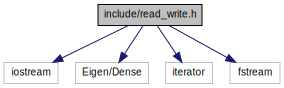
\includegraphics[width=350pt]{read__write_8h__incl}
\end{center}
\end{figure}
\-This graph shows which files directly or indirectly include this file\-:
\nopagebreak
\begin{figure}[H]
\begin{center}
\leavevmode
\includegraphics[width=350pt]{read__write_8h__dep__incl}
\end{center}
\end{figure}
\subsection*{\-Namespaces}
\begin{DoxyCompactItemize}
\item 
namespace \hyperlink{namespacelibcnn}{libcnn}
\end{DoxyCompactItemize}
\subsection*{\-Functions}
\begin{DoxyCompactItemize}
\item 
{\footnotesize template$<$class Matrix $>$ }\\void \hyperlink{namespacelibcnn_ab9d1cc7fff65924fba4673d248ce5b84}{libcnn\-::write\-\_\-binary} (const char $\ast$filename, const \-Matrix \&matrix)
\item 
{\footnotesize template$<$class Matrix $>$ }\\void \hyperlink{namespacelibcnn_a08fddcf34488abeb9551fa4ba5f69b02}{libcnn\-::read\-\_\-binary} (const char $\ast$filename, \-Matrix \&matrix)
\end{DoxyCompactItemize}

\input{save__load_8h}
\hypertarget{get__klt__kernels_8m}{\section{matlab/kernels/get\-\_\-klt\-\_\-kernels.m \-File \-Reference}
\label{get__klt__kernels_8m}\index{matlab/kernels/get\-\_\-klt\-\_\-kernels.\-m@{matlab/kernels/get\-\_\-klt\-\_\-kernels.\-m}}
}
\subsection*{\-Functions}
\begin{DoxyCompactItemize}
\item 
\hyperlink{get__klt__kernels_8m_a1c9fd3c594d02062b3ac5cf712d90f8f}{subim\-\_\-} (\-:,\-:, \hyperlink{map__label__image_8m_a6f6ccfcf58b31cb6412107d9d5281426}{i})
\item 
\hyperlink{get__klt__kernels_8m_aa140f697e3b9bb2f7ba316a325f6c912}{figure} ('\-Position',\mbox{[}100 100 700 650\mbox{]})
\item 
for \hyperlink{get__klt__kernels_8m_ab3c390c8309e35a62c02e7342b599355}{subplot} (\hyperlink{get__klt__kernels_8m_aa4a403ed34dcccddf769c6c6709ccb85}{n}, \hyperlink{get__klt__kernels_8m_aa4a403ed34dcccddf769c6c6709ccb85}{n}, \hyperlink{map__label__image_8m_a6f6ccfcf58b31cb6412107d9d5281426}{i})
\item 
\hyperlink{get__klt__kernels_8m_acb7f26dfddf92958620c26619872a11b}{imagesc} (\hyperlink{get__klt__kernels_8m_a16e4ef534cec559430e07e05eb71c719}{\-K}(\-:,\-:, \hyperlink{map__label__image_8m_a6f6ccfcf58b31cb6412107d9d5281426}{i}))
\item 
colormap \hyperlink{rand__lr005_2test6_8m_ada8ad40249884b4f8e370f25724a131f}{gray} end \hyperlink{get__klt__kernels_8m_ab638a7a5d0720819296aa048fc4f5907}{title} (sprintf('\%\hyperlink{get__klt__kernels_8m_a3691308f2a4c2f6983f2880d32e29c84}{s}', \hyperlink{get__klt__kernels_8m_ad0ee599b1ec66f009a9a92d13e140b1e}{image\-\_\-filename}))
\end{DoxyCompactItemize}
\subsection*{\-Variables}
\begin{DoxyCompactItemize}
\item 
function \hyperlink{get__klt__kernels_8m_a16e4ef534cec559430e07e05eb71c719}{\-K}
\item 
function \hyperlink{get__klt__kernels_8m_aa4a403ed34dcccddf769c6c6709ccb85}{n} = 7
\item 
\hyperlink{get__klt__kernels_8m_ad0ee599b1ec66f009a9a92d13e140b1e}{image\-\_\-filename} = '1.jpg'
\item 
elseif \hyperlink{get__klt__kernels_8m_a8b840739d323b6d3e5eccbbef6043558}{nargin} = = 1
\item 
end \hyperlink{get__klt__kernels_8m_a731676ea925e67f45c143fcf877dcb4c}{n\-\_\-sample} = 10$\ast$\hyperlink{get__klt__kernels_8m_aa4a403ed34dcccddf769c6c6709ccb85}{n}$\ast$\hyperlink{get__klt__kernels_8m_aa4a403ed34dcccddf769c6c6709ccb85}{n}
\item 
\hyperlink{get__klt__kernels_8m_a36aff75e89a0f2a99eca767b6ece034d}{im} = imread(\hyperlink{get__klt__kernels_8m_ad0ee599b1ec66f009a9a92d13e140b1e}{image\-\_\-filename})
\item 
\hyperlink{get__klt__kernels_8m_afe48d1d4f923c59f25255796d824a0e9}{im\-\_\-g} = rgb2gray(\hyperlink{get__klt__kernels_8m_a36aff75e89a0f2a99eca767b6ece034d}{im})
\item 
\hyperlink{get__klt__kernels_8m_a3691308f2a4c2f6983f2880d32e29c84}{s} = size(\hyperlink{get__klt__kernels_8m_a36aff75e89a0f2a99eca767b6ece034d}{im})
\item 
array of samples \hyperlink{get__klt__kernels_8m_ac5daebc4a595d193caa16862da3b170a}{subim\-\_\-} = zeros(\hyperlink{get__klt__kernels_8m_aa4a403ed34dcccddf769c6c6709ccb85}{n},\hyperlink{get__klt__kernels_8m_aa4a403ed34dcccddf769c6c6709ccb85}{n},\hyperlink{get__klt__kernels_8m_a731676ea925e67f45c143fcf877dcb4c}{n\-\_\-sample})
\item 
\hyperlink{get__klt__kernels_8m_a52324bcb04289fe3f876139bc74c6c30}{subim} = zeros(\hyperlink{get__klt__kernels_8m_aa4a403ed34dcccddf769c6c6709ccb85}{n},\hyperlink{get__klt__kernels_8m_aa4a403ed34dcccddf769c6c6709ccb85}{n},\hyperlink{get__klt__kernels_8m_a731676ea925e67f45c143fcf877dcb4c}{n\-\_\-sample})
\item 
substract mean for \hyperlink{get__klt__kernels_8m_a81b94ba50b782836960e54bcfa99fc88}{i} = 1\-:\hyperlink{get__klt__kernels_8m_a731676ea925e67f45c143fcf877dcb4c}{n\-\_\-sample}
\item 
substract mean for \hyperlink{get__klt__kernels_8m_aa6f55716b4169c96bd748a1949af521b}{r} = randi(\hyperlink{get__klt__kernels_8m_a3691308f2a4c2f6983f2880d32e29c84}{s}(1)-\/\hyperlink{get__klt__kernels_8m_aa4a403ed34dcccddf769c6c6709ccb85}{n}-\/1)
\item 
\hyperlink{get__klt__kernels_8m_ae0323a9039add2978bf5b49550572c7c}{c} = randi(\hyperlink{get__klt__kernels_8m_a3691308f2a4c2f6983f2880d32e29c84}{s}(2)-\/\hyperlink{get__klt__kernels_8m_aa4a403ed34dcccddf769c6c6709ccb85}{n}-\/1)
\item 
end \hyperlink{get__klt__kernels_8m_a1932ab2c985b9f56e67dd2b747c3aaa7}{im\-\_\-mean} = mean(\hyperlink{get__klt__kernels_8m_a1c9fd3c594d02062b3ac5cf712d90f8f}{subim\-\_\-},3)
\item 
image data as vectors \hyperlink{get__klt__kernels_8m_aa8421c649b51de89db65bf81df358fd6}{image\-\_\-vectors} = reshape(\hyperlink{get__klt__kernels_8m_a52324bcb04289fe3f876139bc74c6c30}{subim}, \hyperlink{get__klt__kernels_8m_aa4a403ed34dcccddf769c6c6709ccb85}{n}$\ast$\hyperlink{get__klt__kernels_8m_aa4a403ed34dcccddf769c6c6709ccb85}{n}, \hyperlink{get__klt__kernels_8m_a731676ea925e67f45c143fcf877dcb4c}{n\-\_\-sample})
\item 
covariance \hyperlink{get__klt__kernels_8m_ae587c08ca7bc00fe7739a3ecf276a2cf}{\-Cov} = \hyperlink{get__klt__kernels_8m_aa8421c649b51de89db65bf81df358fd6}{image\-\_\-vectors} $\ast$ \hyperlink{get__klt__kernels_8m_aa8421c649b51de89db65bf81df358fd6}{image\-\_\-vectors}'
\item 
\hyperlink{get__klt__kernels_8m_a0811656e57ca05d05abeb43b41eb11a7}{decompose} \mbox{[}u, \hyperlink{yaml__t__load_8cpp_a80d599bd22867a8e610e0be09bf1128d}{v}\mbox{]} = eig(\hyperlink{get__klt__kernels_8m_ae587c08ca7bc00fe7739a3ecf276a2cf}{\-Cov})
\end{DoxyCompactItemize}


\subsection{\-Function \-Documentation}
\hypertarget{get__klt__kernels_8m_aa140f697e3b9bb2f7ba316a325f6c912}{\index{get\-\_\-klt\-\_\-kernels.\-m@{get\-\_\-klt\-\_\-kernels.\-m}!figure@{figure}}
\index{figure@{figure}!get_klt_kernels.m@{get\-\_\-klt\-\_\-kernels.\-m}}
\subsubsection[{figure}]{\setlength{\rightskip}{0pt plus 5cm}{\bf figure} (
\begin{DoxyParamCaption}
\item[{'\-Position'}]{}
\end{DoxyParamCaption}
)}}\label{get__klt__kernels_8m_aa140f697e3b9bb2f7ba316a325f6c912}
\hypertarget{get__klt__kernels_8m_acb7f26dfddf92958620c26619872a11b}{\index{get\-\_\-klt\-\_\-kernels.\-m@{get\-\_\-klt\-\_\-kernels.\-m}!imagesc@{imagesc}}
\index{imagesc@{imagesc}!get_klt_kernels.m@{get\-\_\-klt\-\_\-kernels.\-m}}
\subsubsection[{imagesc}]{\setlength{\rightskip}{0pt plus 5cm}{\bf imagesc} (
\begin{DoxyParamCaption}
\item[{{\bf \-K}(\-:,\-:, {\bf i})}]{}
\end{DoxyParamCaption}
)}}\label{get__klt__kernels_8m_acb7f26dfddf92958620c26619872a11b}
\hypertarget{get__klt__kernels_8m_a1c9fd3c594d02062b3ac5cf712d90f8f}{\index{get\-\_\-klt\-\_\-kernels.\-m@{get\-\_\-klt\-\_\-kernels.\-m}!subim\-\_\-@{subim\-\_\-}}
\index{subim\-\_\-@{subim\-\_\-}!get_klt_kernels.m@{get\-\_\-klt\-\_\-kernels.\-m}}
\subsubsection[{subim\-\_\-}]{\setlength{\rightskip}{0pt plus 5cm}{\bf subim\-\_\-} (
\begin{DoxyParamCaption}
\item[{\-:}]{, }
\item[{\-:}]{, }
\item[{{\bf i}}]{}
\end{DoxyParamCaption}
)}}\label{get__klt__kernels_8m_a1c9fd3c594d02062b3ac5cf712d90f8f}
\hypertarget{get__klt__kernels_8m_ab3c390c8309e35a62c02e7342b599355}{\index{get\-\_\-klt\-\_\-kernels.\-m@{get\-\_\-klt\-\_\-kernels.\-m}!subplot@{subplot}}
\index{subplot@{subplot}!get_klt_kernels.m@{get\-\_\-klt\-\_\-kernels.\-m}}
\subsubsection[{subplot}]{\setlength{\rightskip}{0pt plus 5cm}for {\bf subplot} (
\begin{DoxyParamCaption}
\item[{{\bf n}}]{, }
\item[{{\bf n}}]{, }
\item[{{\bf i}}]{}
\end{DoxyParamCaption}
)}}\label{get__klt__kernels_8m_ab3c390c8309e35a62c02e7342b599355}
\hypertarget{get__klt__kernels_8m_ab638a7a5d0720819296aa048fc4f5907}{\index{get\-\_\-klt\-\_\-kernels.\-m@{get\-\_\-klt\-\_\-kernels.\-m}!title@{title}}
\index{title@{title}!get_klt_kernels.m@{get\-\_\-klt\-\_\-kernels.\-m}}
\subsubsection[{title}]{\setlength{\rightskip}{0pt plus 5cm}colormap {\bf gray} end {\bf title} (
\begin{DoxyParamCaption}
\item[{sprintf('\%{\bf s}', {\bf image\-\_\-filename})}]{}
\end{DoxyParamCaption}
)}}\label{get__klt__kernels_8m_ab638a7a5d0720819296aa048fc4f5907}


\subsection{\-Variable \-Documentation}
\hypertarget{get__klt__kernels_8m_ae0323a9039add2978bf5b49550572c7c}{\index{get\-\_\-klt\-\_\-kernels.\-m@{get\-\_\-klt\-\_\-kernels.\-m}!c@{c}}
\index{c@{c}!get_klt_kernels.m@{get\-\_\-klt\-\_\-kernels.\-m}}
\subsubsection[{c}]{\setlength{\rightskip}{0pt plus 5cm}{\bf c} = randi({\bf s}(2)-\/{\bf n}-\/1)}}\label{get__klt__kernels_8m_ae0323a9039add2978bf5b49550572c7c}
\hypertarget{get__klt__kernels_8m_ae587c08ca7bc00fe7739a3ecf276a2cf}{\index{get\-\_\-klt\-\_\-kernels.\-m@{get\-\_\-klt\-\_\-kernels.\-m}!\-Cov@{\-Cov}}
\index{\-Cov@{\-Cov}!get_klt_kernels.m@{get\-\_\-klt\-\_\-kernels.\-m}}
\subsubsection[{\-Cov}]{\setlength{\rightskip}{0pt plus 5cm}covariance {\bf \-Cov} = {\bf image\-\_\-vectors} $\ast$ {\bf image\-\_\-vectors}'}}\label{get__klt__kernels_8m_ae587c08ca7bc00fe7739a3ecf276a2cf}
\hypertarget{get__klt__kernels_8m_a0811656e57ca05d05abeb43b41eb11a7}{\index{get\-\_\-klt\-\_\-kernels.\-m@{get\-\_\-klt\-\_\-kernels.\-m}!decompose@{decompose}}
\index{decompose@{decompose}!get_klt_kernels.m@{get\-\_\-klt\-\_\-kernels.\-m}}
\subsubsection[{decompose}]{\setlength{\rightskip}{0pt plus 5cm}{\bf decompose}\mbox{[}u, {\bf v}\mbox{]} = eig({\bf \-Cov})}}\label{get__klt__kernels_8m_a0811656e57ca05d05abeb43b41eb11a7}
\hypertarget{get__klt__kernels_8m_a81b94ba50b782836960e54bcfa99fc88}{\index{get\-\_\-klt\-\_\-kernels.\-m@{get\-\_\-klt\-\_\-kernels.\-m}!i@{i}}
\index{i@{i}!get_klt_kernels.m@{get\-\_\-klt\-\_\-kernels.\-m}}
\subsubsection[{i}]{\setlength{\rightskip}{0pt plus 5cm}end for {\bf i} = 1\-:{\bf n\-\_\-sample}}}\label{get__klt__kernels_8m_a81b94ba50b782836960e54bcfa99fc88}
\hypertarget{get__klt__kernels_8m_a36aff75e89a0f2a99eca767b6ece034d}{\index{get\-\_\-klt\-\_\-kernels.\-m@{get\-\_\-klt\-\_\-kernels.\-m}!im@{im}}
\index{im@{im}!get_klt_kernels.m@{get\-\_\-klt\-\_\-kernels.\-m}}
\subsubsection[{im}]{\setlength{\rightskip}{0pt plus 5cm}{\bf im} = imread({\bf image\-\_\-filename})}}\label{get__klt__kernels_8m_a36aff75e89a0f2a99eca767b6ece034d}
\hypertarget{get__klt__kernels_8m_afe48d1d4f923c59f25255796d824a0e9}{\index{get\-\_\-klt\-\_\-kernels.\-m@{get\-\_\-klt\-\_\-kernels.\-m}!im\-\_\-g@{im\-\_\-g}}
\index{im\-\_\-g@{im\-\_\-g}!get_klt_kernels.m@{get\-\_\-klt\-\_\-kernels.\-m}}
\subsubsection[{im\-\_\-g}]{\setlength{\rightskip}{0pt plus 5cm}{\bf im\-\_\-g} = rgb2gray({\bf im})}}\label{get__klt__kernels_8m_afe48d1d4f923c59f25255796d824a0e9}
\hypertarget{get__klt__kernels_8m_a1932ab2c985b9f56e67dd2b747c3aaa7}{\index{get\-\_\-klt\-\_\-kernels.\-m@{get\-\_\-klt\-\_\-kernels.\-m}!im\-\_\-mean@{im\-\_\-mean}}
\index{im\-\_\-mean@{im\-\_\-mean}!get_klt_kernels.m@{get\-\_\-klt\-\_\-kernels.\-m}}
\subsubsection[{im\-\_\-mean}]{\setlength{\rightskip}{0pt plus 5cm}end {\bf im\-\_\-mean} = mean({\bf subim\-\_\-},3)}}\label{get__klt__kernels_8m_a1932ab2c985b9f56e67dd2b747c3aaa7}
\hypertarget{get__klt__kernels_8m_ad0ee599b1ec66f009a9a92d13e140b1e}{\index{get\-\_\-klt\-\_\-kernels.\-m@{get\-\_\-klt\-\_\-kernels.\-m}!image\-\_\-filename@{image\-\_\-filename}}
\index{image\-\_\-filename@{image\-\_\-filename}!get_klt_kernels.m@{get\-\_\-klt\-\_\-kernels.\-m}}
\subsubsection[{image\-\_\-filename}]{\setlength{\rightskip}{0pt plus 5cm}{\bf image\-\_\-filename} = '1.jpg'}}\label{get__klt__kernels_8m_ad0ee599b1ec66f009a9a92d13e140b1e}
\hypertarget{get__klt__kernels_8m_aa8421c649b51de89db65bf81df358fd6}{\index{get\-\_\-klt\-\_\-kernels.\-m@{get\-\_\-klt\-\_\-kernels.\-m}!image\-\_\-vectors@{image\-\_\-vectors}}
\index{image\-\_\-vectors@{image\-\_\-vectors}!get_klt_kernels.m@{get\-\_\-klt\-\_\-kernels.\-m}}
\subsubsection[{image\-\_\-vectors}]{\setlength{\rightskip}{0pt plus 5cm}image data as vectors {\bf image\-\_\-vectors} = reshape({\bf subim}, {\bf n}$\ast${\bf n}, {\bf n\-\_\-sample})}}\label{get__klt__kernels_8m_aa8421c649b51de89db65bf81df358fd6}
\hypertarget{get__klt__kernels_8m_a16e4ef534cec559430e07e05eb71c719}{\index{get\-\_\-klt\-\_\-kernels.\-m@{get\-\_\-klt\-\_\-kernels.\-m}!\-K@{\-K}}
\index{\-K@{\-K}!get_klt_kernels.m@{get\-\_\-klt\-\_\-kernels.\-m}}
\subsubsection[{\-K}]{\setlength{\rightskip}{0pt plus 5cm}{\bf \-K}}}\label{get__klt__kernels_8m_a16e4ef534cec559430e07e05eb71c719}
{\bfseries \-Initial value\-:}
\begin{DoxyCode}
get_klt_kernels(image_filename,n)
% @n is the output dimension of Kernels
% @n_sample is the number of samples extract from image
%
% @K: computed kernels

if nargin == 0
\end{DoxyCode}
\hypertarget{get__klt__kernels_8m_aa4a403ed34dcccddf769c6c6709ccb85}{\index{get\-\_\-klt\-\_\-kernels.\-m@{get\-\_\-klt\-\_\-kernels.\-m}!n@{n}}
\index{n@{n}!get_klt_kernels.m@{get\-\_\-klt\-\_\-kernels.\-m}}
\subsubsection[{n}]{\setlength{\rightskip}{0pt plus 5cm}elseif {\bf n} = 7}}\label{get__klt__kernels_8m_aa4a403ed34dcccddf769c6c6709ccb85}
\hypertarget{get__klt__kernels_8m_a731676ea925e67f45c143fcf877dcb4c}{\index{get\-\_\-klt\-\_\-kernels.\-m@{get\-\_\-klt\-\_\-kernels.\-m}!n\-\_\-sample@{n\-\_\-sample}}
\index{n\-\_\-sample@{n\-\_\-sample}!get_klt_kernels.m@{get\-\_\-klt\-\_\-kernels.\-m}}
\subsubsection[{n\-\_\-sample}]{\setlength{\rightskip}{0pt plus 5cm}end {\bf n\-\_\-sample} = 10$\ast${\bf n}$\ast${\bf n}}}\label{get__klt__kernels_8m_a731676ea925e67f45c143fcf877dcb4c}
\hypertarget{get__klt__kernels_8m_a8b840739d323b6d3e5eccbbef6043558}{\index{get\-\_\-klt\-\_\-kernels.\-m@{get\-\_\-klt\-\_\-kernels.\-m}!nargin@{nargin}}
\index{nargin@{nargin}!get_klt_kernels.m@{get\-\_\-klt\-\_\-kernels.\-m}}
\subsubsection[{nargin}]{\setlength{\rightskip}{0pt plus 5cm}elseif {\bf nargin} = = 1}}\label{get__klt__kernels_8m_a8b840739d323b6d3e5eccbbef6043558}
\hypertarget{get__klt__kernels_8m_aa6f55716b4169c96bd748a1949af521b}{\index{get\-\_\-klt\-\_\-kernels.\-m@{get\-\_\-klt\-\_\-kernels.\-m}!r@{r}}
\index{r@{r}!get_klt_kernels.m@{get\-\_\-klt\-\_\-kernels.\-m}}
\subsubsection[{r}]{\setlength{\rightskip}{0pt plus 5cm}substract mean for {\bf r} = randi({\bf s}(1)-\/{\bf n}-\/1)}}\label{get__klt__kernels_8m_aa6f55716b4169c96bd748a1949af521b}
\hypertarget{get__klt__kernels_8m_a3691308f2a4c2f6983f2880d32e29c84}{\index{get\-\_\-klt\-\_\-kernels.\-m@{get\-\_\-klt\-\_\-kernels.\-m}!s@{s}}
\index{s@{s}!get_klt_kernels.m@{get\-\_\-klt\-\_\-kernels.\-m}}
\subsubsection[{s}]{\setlength{\rightskip}{0pt plus 5cm}{\bf s} = size({\bf im})}}\label{get__klt__kernels_8m_a3691308f2a4c2f6983f2880d32e29c84}
\hypertarget{get__klt__kernels_8m_a52324bcb04289fe3f876139bc74c6c30}{\index{get\-\_\-klt\-\_\-kernels.\-m@{get\-\_\-klt\-\_\-kernels.\-m}!subim@{subim}}
\index{subim@{subim}!get_klt_kernels.m@{get\-\_\-klt\-\_\-kernels.\-m}}
\subsubsection[{subim}]{\setlength{\rightskip}{0pt plus 5cm}{\bf subim} = zeros({\bf n},{\bf n},{\bf n\-\_\-sample})}}\label{get__klt__kernels_8m_a52324bcb04289fe3f876139bc74c6c30}
\hypertarget{get__klt__kernels_8m_ac5daebc4a595d193caa16862da3b170a}{\index{get\-\_\-klt\-\_\-kernels.\-m@{get\-\_\-klt\-\_\-kernels.\-m}!subim\-\_\-@{subim\-\_\-}}
\index{subim\-\_\-@{subim\-\_\-}!get_klt_kernels.m@{get\-\_\-klt\-\_\-kernels.\-m}}
\subsubsection[{subim\-\_\-}]{\setlength{\rightskip}{0pt plus 5cm}array of samples {\bf subim\-\_\-} = zeros({\bf n},{\bf n},{\bf n\-\_\-sample})}}\label{get__klt__kernels_8m_ac5daebc4a595d193caa16862da3b170a}

\hypertarget{runtest_8m}{\section{matlab/kernels/runtest.m \-File \-Reference}
\label{runtest_8m}\index{matlab/kernels/runtest.\-m@{matlab/kernels/runtest.\-m}}
}
\subsection*{\-Functions}
\begin{DoxyCompactItemize}
\item 
\hyperlink{runtest_8m_aee8a3839e598401b379cb62659cd1cbe}{get\-\_\-klt\-\_\-kernels} ('1.jpg') \hyperlink{runtest_8m_ae16ee88a57f1bf74ff3a109c89c66fa2}{get\-\_\-klt\-\_\-kernels}('2.jpg') \hyperlink{runtest_8m_ae16ee88a57f1bf74ff3a109c89c66fa2}{get\-\_\-klt\-\_\-kernels}('3.jpg')
\item 
\hyperlink{runtest_8m_a4967783720139ed2bbfea45578f12799}{get\-\_\-klt\-\_\-kernels} ('4.jpg')
\item 
\hyperlink{runtest_8m_a34048bec12e9f292d699937d6102b6cb}{get\-\_\-klt\-\_\-kernels} ('5.jpg')
\item 
\hyperlink{runtest_8m_ae16ee88a57f1bf74ff3a109c89c66fa2}{get\-\_\-klt\-\_\-kernels} ('6.jpg')
\end{DoxyCompactItemize}


\subsection{\-Function \-Documentation}
\hypertarget{runtest_8m_aee8a3839e598401b379cb62659cd1cbe}{\index{runtest.\-m@{runtest.\-m}!get\-\_\-klt\-\_\-kernels@{get\-\_\-klt\-\_\-kernels}}
\index{get\-\_\-klt\-\_\-kernels@{get\-\_\-klt\-\_\-kernels}!runtest.m@{runtest.\-m}}
\subsubsection[{get\-\_\-klt\-\_\-kernels}]{\setlength{\rightskip}{0pt plus 5cm}{\bf get\-\_\-klt\-\_\-kernels} (
\begin{DoxyParamCaption}
\item[{'1.jpg'}]{}
\end{DoxyParamCaption}
)}}\label{runtest_8m_aee8a3839e598401b379cb62659cd1cbe}
\hypertarget{runtest_8m_a4967783720139ed2bbfea45578f12799}{\index{runtest.\-m@{runtest.\-m}!get\-\_\-klt\-\_\-kernels@{get\-\_\-klt\-\_\-kernels}}
\index{get\-\_\-klt\-\_\-kernels@{get\-\_\-klt\-\_\-kernels}!runtest.m@{runtest.\-m}}
\subsubsection[{get\-\_\-klt\-\_\-kernels}]{\setlength{\rightskip}{0pt plus 5cm}{\bf get\-\_\-klt\-\_\-kernels} (
\begin{DoxyParamCaption}
\item[{'4.jpg'}]{}
\end{DoxyParamCaption}
)}}\label{runtest_8m_a4967783720139ed2bbfea45578f12799}
\hypertarget{runtest_8m_a34048bec12e9f292d699937d6102b6cb}{\index{runtest.\-m@{runtest.\-m}!get\-\_\-klt\-\_\-kernels@{get\-\_\-klt\-\_\-kernels}}
\index{get\-\_\-klt\-\_\-kernels@{get\-\_\-klt\-\_\-kernels}!runtest.m@{runtest.\-m}}
\subsubsection[{get\-\_\-klt\-\_\-kernels}]{\setlength{\rightskip}{0pt plus 5cm}{\bf get\-\_\-klt\-\_\-kernels} (
\begin{DoxyParamCaption}
\item[{'5.jpg'}]{}
\end{DoxyParamCaption}
)}}\label{runtest_8m_a34048bec12e9f292d699937d6102b6cb}
\hypertarget{runtest_8m_ae16ee88a57f1bf74ff3a109c89c66fa2}{\index{runtest.\-m@{runtest.\-m}!get\-\_\-klt\-\_\-kernels@{get\-\_\-klt\-\_\-kernels}}
\index{get\-\_\-klt\-\_\-kernels@{get\-\_\-klt\-\_\-kernels}!runtest.m@{runtest.\-m}}
\subsubsection[{get\-\_\-klt\-\_\-kernels}]{\setlength{\rightskip}{0pt plus 5cm}{\bf get\-\_\-klt\-\_\-kernels} (
\begin{DoxyParamCaption}
\item[{'6.jpg'}]{}
\end{DoxyParamCaption}
)}}\label{runtest_8m_ae16ee88a57f1bf74ff3a109c89c66fa2}

\hypertarget{confusion_8m}{\section{matlab/visualize/confusion.m \-File \-Reference}
\label{confusion_8m}\index{matlab/visualize/confusion.\-m@{matlab/visualize/confusion.\-m}}
}
\subsection*{\-Variables}
\begin{DoxyCompactItemize}
\item 
function \hyperlink{confusion_8m_a77c71ef956b536f6e6bc4b1898ca2e99}{con\-\_\-mat}
\item 
for \hyperlink{confusion_8m_a81b94ba50b782836960e54bcfa99fc88}{i}
\end{DoxyCompactItemize}


\subsection{\-Variable \-Documentation}
\hypertarget{confusion_8m_a77c71ef956b536f6e6bc4b1898ca2e99}{\index{confusion.\-m@{confusion.\-m}!con\-\_\-mat@{con\-\_\-mat}}
\index{con\-\_\-mat@{con\-\_\-mat}!confusion.m@{confusion.\-m}}
\subsubsection[{con\-\_\-mat}]{\setlength{\rightskip}{0pt plus 5cm}function {\bf con\-\_\-mat}}}\label{confusion_8m_a77c71ef956b536f6e6bc4b1898ca2e99}
{\bfseries \-Initial value\-:}
\begin{DoxyCode}
 confusion(predicted, truth, num_labels)

con_mat = zeros(num_labels, num_labels)
\end{DoxyCode}
\hypertarget{confusion_8m_a81b94ba50b782836960e54bcfa99fc88}{\index{confusion.\-m@{confusion.\-m}!i@{i}}
\index{i@{i}!confusion.m@{confusion.\-m}}
\subsubsection[{i}]{\setlength{\rightskip}{0pt plus 5cm}end for {\bf i}}}\label{confusion_8m_a81b94ba50b782836960e54bcfa99fc88}
{\bfseries \-Initial value\-:}
\begin{DoxyCode}
 1: length(predicted)
    con_mat(truth(i) + 1, predicted(i) + 1) = con_mat(truth(i) + 1, predicted(i
      ) + 1) + 1
\end{DoxyCode}

\hypertarget{map__label__color_8m}{\section{matlab/visualize/map\-\_\-label\-\_\-color.m \-File \-Reference}
\label{map__label__color_8m}\index{matlab/visualize/map\-\_\-label\-\_\-color.\-m@{matlab/visualize/map\-\_\-label\-\_\-color.\-m}}
}
\subsection*{\-Variables}
\begin{DoxyCompactItemize}
\item 
function \hyperlink{map__label__color_8m_acfdaec9102228bc59f6d1897bb6bd354}{color}
\end{DoxyCompactItemize}


\subsection{\-Variable \-Documentation}
\hypertarget{map__label__color_8m_acfdaec9102228bc59f6d1897bb6bd354}{\index{map\-\_\-label\-\_\-color.\-m@{map\-\_\-label\-\_\-color.\-m}!color@{color}}
\index{color@{color}!map_label_color.m@{map\-\_\-label\-\_\-color.\-m}}
\subsubsection[{color}]{\setlength{\rightskip}{0pt plus 5cm}yellow case unknown {\bf color}}}\label{map__label__color_8m_acfdaec9102228bc59f6d1897bb6bd354}
{\bfseries \-Initial value\-:}
\begin{DoxyCode}
 map_label_color(label)
    switch label
        case 0                              % sky
            color = [0 0 255]
\end{DoxyCode}

\input{map__label__image_8m}
\hypertarget{result_8m}{\section{matlab/visualize/result.m \-File \-Reference}
\label{result_8m}\index{matlab/visualize/result.\-m@{matlab/visualize/result.\-m}}
}
\subsection*{\-Variables}
\begin{DoxyCompactItemize}
\item 
\hyperlink{result_8m_a75d4f74317ef3f6936b5b49e3df1ee97}{pred}
\item 
\hyperlink{result_8m_adaaf0852d00b6679e5e09de32cf224f9}{accu}
\end{DoxyCompactItemize}


\subsection{\-Variable \-Documentation}
\hypertarget{result_8m_adaaf0852d00b6679e5e09de32cf224f9}{\index{result.\-m@{result.\-m}!accu@{accu}}
\index{accu@{accu}!result.m@{result.\-m}}
\subsubsection[{accu}]{\setlength{\rightskip}{0pt plus 5cm}{\bf accu}}}\label{result_8m_adaaf0852d00b6679e5e09de32cf224f9}
{\bfseries \-Initial value\-:}
\begin{DoxyCode}
 [ 0 0 0 0 0 0 0 0 0 0 0 0 0 0 0 0 0 0 0 0 0 0 0 0 0 0 0 0 0 0 0 0 0 0 0 0 0 0 
      0 0 0 0 0 0 0 0 0 0 0 0 0 0 0 0 0 0 0 0 0 0 0 0 0 0 0 0 0 0 0 0 0 0 0 0 0 0 0 0 
      0 0 0 0 0 0 0 0 0 0 0 0 0 0 0 0 0 0 0 0 0 0 0 0 0 0 0 0 0 0 0 0 0 0 0 0 0 0 0 0 
      0 0 0 0 0 0 0 0 0 0 0 0 0 0 0 0 0 0 0 0 0 0 0 0 0 0 0 0 0 0 0 0 0 0 0 0 0 0 0 0 
      0 0 0 0 0 0 0 0 0 0 0 0 0 0 0 0 0 0 0 0 0 0 0 0 0 0 0 0 0 0 0 0 0 0 0 0 0 0 0 0 
      0 0 0 0 0 0 0 0 0 0 5 0 0 0 0 0 0 0 0 0 0 0 0 0 0 0 0 0 0 0 0 0 0 0 0 0 0 0 5 5 
      5 5 0 0 0 0 0 0 0 0 0 0 0 0 0 0 0 0 0 0 0 0 0 5 5 5 5 5 5 5 5 5 0 0 0 0 0 0 0 0 
      0 0 0 5 5 5 5 5 5 5 5 5 5 5 5 5 5 5 5 5 5 5 0 5 5 5 0 0 0 0 0 5 5 5 5 5 5 5 5 5 
      5 5 5 5 5 5 5 5 5 5 5 5 5 5 5 5 5 5 0 0 5 5 5 5 5 5 5 5 5 5 5 5 5 5 5 5 5 5 5 5 
      5 5 5 5 5 5 5 5 1 1 5 5 5 5 5 1 1 1 5 5 5 5 5 5 5 5 5 5 5 5 5 5 5 5 5 5 1 1 1 1 
      1 5 5 5 1 1 1 1 1 1 5 5 5 5 5 5 5 5 5 5 5 5 5 5 1 1 1 1 1 1 1 5 5 5 1 1 1 1 1 1 
      5 5 5 5 5 5 5 5 5 5 5 5 5 5 1 1 1 1 1 1 1 5 5 1 1 1 1 1 1 1 1 5 5 5 5 5 5 5 5 5 
      5 5 8 1 1 1 1 1 1 1 1 5 5 1 1 1 1 1 1 1 1 1 5 5 5 5 5 5 5 5 5 5 8 1 1 1 1 1 1 1 
      1 5 5 1 1 1 1 1 1 1 1 5 5 5 5 5 5 5 5 5 5 5 8 8 1 1 1 1 1 1 1 5 5 1 1 1 1 1 1 1 
      5 5 5 5 5 5 5 5 5 5 5 5 8 8 1 1 1 1 1 1 5 5 5 1 1 1 1 1 1 1 5 5 5 5 5 5 5 5 5 5 
      5 8 3 3 3 1 1 1 1 8 8 5 5 5 1 1 1 5 5 5 5 5 5 5 5 5 5 5 5 5 8 8 3 3 3 3 3 3 3 3 
      3 3 3 3 3 3 3 3 8 8 8 5 5 5 5 5 5 8 8 8 8 8 3 3 3 3 3 3 3 3 3 3 3 3 3 3 3 3 3 3 
      3 3 3 3 3 3 3 3 8 8 8 8 3 3 3 3 3 3 3 3 3 3 3 3 3 3 3 3 3 3 3 3 3 3 3 3 3 3 3 3 
      3 3 3 3 3 3 3 3 3 3 3 3 3 3 3 3 3 3 3 3 3 3 3 3 3 3 3 3 3 3 3 3 3 3 3 3 3 3 3 3 
      3 3 3 3 3 3 3 3 3 3 3 3 3 3 3 3 3 3 3 3 3 3 3 3 3 3 3 3 3 3 3 3 3 3 3 3 3 3 3 3 
      3 3 3 3 3 3 3 3 3 3 3 3 3 3 3 3 3 3 3 3 3 3 3 3 3 3 3 3 3 3 3 3 3 3 3 3 3 3 3 3 
      3 3 3 3 3 3 3 3 3 3 3 3 3 3 3 3 3 3 3 3 3 3 3 3 3 3 3 3 3 3 3 3 3 3 3 3 3 3 3 3 
      3 3 3 3 3 3 3 3 3 3 3 3 3 3 3 3 3 3 3 3 3 3 3 3 3 3 3 3 3 3 3 3 3 3 3 3 3 3 3 3 
      3 3 3 3 3 3 3 3 3 3 2 2 3 3 3 3 3 3 3 3 3 3 3 3 3 3 3 3 3 3 3 3 3 3 3 3 3 3 3 2 
      2 2 3 3 3 3 3 3 3 3 3 3 3 3 3 3 3 3 3 3 3 3 3 3 3 3 3 2 2 2 2 2 2 2 2 2 2 2 2 3 
      3 3 3 3 3 3 3 3 3 3 3 3 3 3 3 2 2 2 2 2 2 2 2 2 2 2 2 2 2 2 2 2 2 2 2 2 2 2 8 8 
      8 8 2 2 2 2 2 2 2 2 2 2 2 2 2 2 2 2 2 2 2 2 2 2 2 2 2 2 2 2 2 2 2 2 2 2 2 2 2 2 
      2 2 2 2 2 2 2 2 2 2 2 2 2 2 2 2 2 2 2 2 2 2 2 2 2 2 2 2 2 2 2 2 2 2 2 2 2 2 2 2 
      2 2 2 2 2 2 2 2 2 2 2 2 2 2 2 2 2 2 2 2 2 2 2 2 2 2 2 2 2 2 2 2 2 2 2 2 2 2 2 2 
      2 2 2 2 2 2 2 2 2 2 2 2 2 2 2 2 2 2 2 2 2 2 2 2 2 2 2 2 2 2 2 2 2 2 2 2 2 2 2 2 
      2 2 8 8 8 8 8 8 8 8 8 8 8 8 8 8 8 8 8 8 8 8 8 8 8 8 8 8 8 8 8 8 8 0 0 0 0 0 0 0 
      0 0 0 0 0 0 0 0 0 0 0 0 0 0 0 0 0 0 0 0 0 0 8 0 0 0 0 0 0 0 0 0 0 0 0 0 0 0 0 0 
      0 0 0 0 0 0 0 0 0 0 0 0 8 0 0 0 0 0 0 0 0 0 0 0 0 0 0 0 0 0 0 0 0 0 0 0 0 0 0 0 
      0 0 8 0 0 0 0 0 0 0 0 0 0 0 0 0 0 0 0 0 0 0 0 0 0 0 0 0 0 0 0 0 8 0 0 0 0 0 0 0 
      0 0 0 0 0 0 0 0 0 0 0 0 0 0 0 0 0 0 0 0 0 0 8 0 0 0 0 0 0 0 0 0 0 0 0 0 0 0 0 0 
      0 0 0 0 0 0 0 0 0 0 0 0 8 0 0 0 0 0 0 0 0 0 0 0 0 0 0 0 0 0 0 0 0 0 0 0 0 0 0 0 
      0 0 8 0 0 0 5 5 0 0 0 0 0 0 0 0 0 0 0 0 0 0 0 0 0 0 0 0 0 0 0 0 5 5 5 5 5 5 0 0 
      0 0 0 0 0 0 0 1 0 0 0 0 0 0 0 0 0 0 0 0 0 0 5 5 5 5 5 5 5 5 5 5 5 1 0 0 1 1 1 0 
      8 8 1 1 0 0 0 0 0 0 0 0 5 5 5 5 5 5 5 5 5 8 8 1 0 8 1 1 1 1 1 1 1 1 1 0 0 0 0 0 
      0 0 5 5 5 5 5 5 5 5 5 1 8 1 0 8 1 1 1 1 1 1 0 1 1 0 0 0 0 0 5 1 5 5 5 5 5 5 5 5 
      8 8 8 1 1 1 1 1 1 1 1 1 5 5 0 0 0 0 5 1 1 1 5 5 5 5 5 5 5 5 5 5 8 1 8 1 1 1 1 1 
      1 8 5 8 5 5 5 5 1 1 1 1 5 5 5 5 5 5 5 8 5 1 1 1 1 1 1 1 1 1 1 5 5 5 5 5 1 1 1 1 
      1 1 5 5 5 5 5 5 5 1 1 1 1 1 1 1 1 1 1 1 1 1 5 5 5 5 5 1 1 1 1 1 5 5 5 5 5 1 1 1 
      1 1 1 1 1 1 1 1 1 1 1 5 5 5 5 5 5 1 1 1 1 1 5 5 5 5 5 1 1 1 1 1 1 1 1 1 1 1 1 1 
      5 5 5 5 5 5 5 1 1 1 5 1 5 5 5 5 5 1 1 1 1 1 1 1 1 1 1 1 1 5 5 5 5 5 5 5 5 5 1 1 
      1 5 5 5 8 8 7 7 8 1 1 1 1 1 1 1 1 1 1 5 5 5 5 5 5 5 5 5 5 1 1 5 5 5 7 7 7 7 7 1 
      1 1 1 1 1 1 1 1 1 1 1 1 5 5 5 5 5 5 5 1 1 5 8 7 7 7 7 7 7 1 1 1 1 1 1 1 1 1 1 1 
      1 1 5 5 5 5 5 5 5 1 1 1 1 3 1 7 7 7 7 1 1 1 1 1 1 1 1 1 1 1 1 1 1 5 5 5 5 5 5 1 
      1 1 1 3 3 3 3 3 2 2 2 2 1 1 1 1 1 1 1 1 1 1 1 1 1 1 1 1 1 1 1 1 1 3 3 3 3 3 3 3 
      3 2 2 2 2 2 2 1 1 1 1 1 1 1 1 1 1 1 1 5 1 1 1 3 3 3 3 3 3 3 3 3 2 2 2 2 2 2 2 2 
      2 2 2 2 2 2 2 2 2 2 2 2 1 3 3 3 3 3 3 3 3 3 2 2 2 2 2 2 2 2 2 2 2 2 2 3 3 3 3 3 
      3 3 1 3 3 3 3 3 3 3 2 2 2 2 2 2 2 2 2 2 2 2 3 3 3 3 3 3 3 3 3 3 1 3 3 3 3 3 3 2 
      2 2 2 2 2 2 2 2 2 2 2 3 3 3 3 3 3 3 3 3 3 3 1 3 3 3 3 2 2 2 2 2 2 2 2 2 2 2 2 2 
      3 3 3 3 3 3 3 3 3 3 3 3 1 3 3 2 2 2 2 2 2 2 2 2 2 2 2 2 2 2 3 3 3 3 3 3 3 3 3 3 
      3 3 1 2 2 2 2 2 2 2 2 2 2 2 2 2 2 2 2 3 3 3 3 3 3 3 3 3 3 3 3 3 1 2 2 2 2 2 2 2 
      2 2 2 2 2 2 2 2 3 3 3 3 3 3 3 3 3 3 3 3 3 3 1 2 2 2 2 2 2 2 2 2 2 2 2 2 2 3 3 3 
      3 3 3 3 3 3 3 3 3 3 3 3 1 2 2 2 2 2 2 2 2 2 2 2 2 2 3 3 3 3 3 3 3 3 3 3 3 3 3 3 
      3 3 1 2 2 2 2 2 2 2 2 2 2 2 2 2 2 3 3 3 3 3 3 3 3 3 3 3 3 3 3 3 2 2 2 2 2 2 2 2 
      2 2 2 2 2 3 3 3 3 3 3 3 3 3 3 3 3 3 3 3 3 3 2 2 2 2 2 2 2 2 2 2 2 2 3 3 3 3 3 3 
      3 3 3 3 3 3 3 3 3 3 3 3 2 2 2 2 2 2 2 2 2 2 2 3 3 3 3 3 3 3 3 3 3 3 3 3 3 3 3 3 
      3 3 8 8 8 8 8 8 8 8 8 8 8 8 8 8 8 8 8 8 8 8 8 8 8 8 8 8 8 8 8 8 8 0 0 0 0 0 0 0 
      0 0 0 0 0 0 0 0 0 0 0 0 0 0 0 0 0 0 0 0 0 0 8 0 0 0 0 0 0 0 0 0 0 0 0 0 0 0 0 0 
      0 0 0 0 0 0 0 0 0 0 0 0 8 0 0 0 0 0 0 0 0 0 0 0 0 0 0 0 0 0 0 0 0 0 0 0 0 0 0 0 
      0 0 8 0 0 0 0 0 0 0 0 0 0 0 0 0 0 0 0 0 0 0 0 0 0 0 0 0 0 0 0 0 8 0 0 0 0 0 0 0 
      0 0 0 0 0 0 0 0 0 0 0 0 0 0 0 0 0 0 0 0 0 0 8 0 0 0 0 0 0 0 0 0 0 0 0 0 0 0 0 0 
      0 0 0 0 0 0 0 0 0 0 0 0 8 0 0 0 0 0 0 0 0 0 0 0 0 0 0 0 0 0 0 0 0 0 0 0 0 0 0 0 
      0 0 8 0 0 0 0 0 0 0 0 0 0 0 0 0 0 0 0 0 0 0 0 0 0 0 0 0 0 0 0 0 8 0 0 0 0 0 0 0 
      0 0 0 0 0 0 0 0 0 0 0 0 0 0 0 0 0 0 0 0 0 0 8 0 0 0 0 0 0 0 0 0 0 0 0 0 0 0 0 0 
      0 0 0 0 0 0 0 0 0 0 0 0 8 0 0 0 0 0 0 0 0 0 0 0 0 0 0 0 0 0 5 5 5 5 5 0 0 0 0 0 
      0 0 8 0 0 0 0 1 1 1 0 1 1 1 1 0 0 0 5 5 5 5 5 5 5 5 5 5 5 5 5 0 8 0 1 1 1 1 1 1 
      1 1 1 1 1 1 5 5 5 5 5 5 5 5 5 5 5 5 5 5 5 5 1 1 1 1 1 1 1 1 1 1 1 1 1 5 5 5 5 5 
      5 5 5 5 5 5 5 5 5 5 5 5 5 1 1 1 1 1 1 1 1 1 1 1 5 5 5 5 5 5 5 5 5 5 5 5 5 5 5 5 
      5 5 5 5 1 1 1 1 1 1 1 1 1 1 5 5 5 5 5 5 5 5 5 5 5 5 5 5 5 5 5 5 5 5 5 1 1 6 1 1 
      1 1 5 6 5 5 5 5 5 5 5 5 5 5 5 5 5 5 5 5 5 5 5 5 5 1 1 1 1 1 5 5 5 6 5 5 5 5 5 5 
      5 5 5 5 5 5 5 5 5 5 5 5 5 5 5 5 5 6 1 5 5 5 1 6 5 5 5 5 5 5 5 5 5 5 5 5 5 5 5 5 
      5 5 5 5 5 5 1 1 1 5 5 5 5 5 5 5 5 5 5 5 5 5 5 5 5 5 5 5 5 5 5 5 5 5 5 5 5 5 5 5 
      5 5 5 5 5 5 5 5 5 5 5 5 5 5 5 5 5 5 5 5 5 5 5 5 5 5 5 5 5 5 5 5 5 5 5 5 5 5 5 5 
      5 5 5 5 5 5 5 5 5 5 5 5 5 5 5 5 5 5 5 5 5 5 5 5 5 5 5 5 5 5 5 5 5 5 5 5 5 5 5 5 
      5 5 5 5 5 5 5 5 5 5 5 5 5 5 5 5 5 5 5 5 5 5 5 5 7 7 7 7 7 7 7 7 5 3 3 3 3 3 3 3 
      5 5 5 5 5 5 5 5 5 5 5 5 5 7 7 7 5 7 5 5 7 5 5 5 5 5 5 5 5 5 5 5 5 5 5 5 5 5 5 5 
      5 5 5 5 5 5 5 5 5 5 5 5 5 3 3 3 3 3 3 3 3 3 3 3 3 3 3 3 3 3 3 5 5 5 5 5 5 5 5 5 
      5 5 5 3 3 3 3 3 3 3 3 3 3 3 3 3 3 3 3 3 3 3 3 3 3 3 3 3 3 3 3 3 5 3 3 3 3 3 3 3 
      3 3 3 3 3 3 3 3 3 3 3 3 3 3 3 3 3 3 3 3 3 3 5 3 3 3 3 3 3 3 3 3 3 3 3 3 3 3 3 3 
      3 3 3 3 3 3 3 3 3 3 3 3 5 3 3 3 3 3 3 3 3 3 3 3 3 3 3 3 3 3 3 3 3 3 3 3 3 3 3 3 
      3 3 5 3 3 3 3 3 3 3 3 3 3 3 3 3 3 3 3 3 3 3 3 3 3 3 3 3 3 3 3 3 5 3 3 3 3 3 3 3 
      3 3 3 3 3 3 3 3 3 3 3 3 3 3 3 3 3 3 3 3 3 3 5 3 3 3 3 3 3 3 3 3 3 3 3 3 3 3 3 3 
      3 3 3 3 3 3 3 3 3 3 3 3 5 3 3 3 3 3 3 3 3 3 3 3 3 3 3 3 3 3 3 3 3 3 3 3 3 3 3 3 
      3 3 5 3 3 3 3 3 3 3 3 3 3 3 3 3 3 3 3 3 3 3 3 3 3 3 3 3 3 3 3 3 5 3 3 3 3 3 3 3 
      3 3 3 3 3 3 3 3 3 3 3 3 3 3 3 3 3 3 3 3 3 3 5 3 3 3 3 3 3 3 3 3 3 3 3 3 3 3 3 3 
      3 3 3 3 3 3 3 3 3 3 3 3 5 3 3 3 3 3 3 3 3 3 3 3 3 3 3 3 3 3 3 3 3 3 3 3 3 3 3 3 
      3 3 0 0 0 0 0 0 0 0 0 0 0 0 0 0 0 0 0 0 0 0 0 0 0 0 0 0 0 0 0 0 0 0 0 0 0 0 0 0 
      0 0 0 0 0 0 0 0 0 0 0 0 0 0 0 0 0 0 0 0 0 0 0 0 0 0 0 0 0 0 0 0 0 0 0 0 0 0 0 0 
      0 0 0 0 0 0 0 0 0 0 0 0 0 0 0 0 0 0 0 0 0 0 0 0 0 0 0 0 0 0 0 0 0 0 0 0 0 0 0 0 
      0 0 0 0 0 0 0 0 0 0 0 0 0 0 0 0 0 0 0 0 0 0 0 0 0 0 0 0 0 0 0 0 0 0 0 0 0 0 0 0 
      0 0 0 0 0 0 0 0 0 0 0 0 0 0 0 0 0 0 0 0 0 0 0 0 0 0 0 0 0 0 0 0 0 0 0 0 0 0 0 0 
      0 0 0 0 0 0 0 0 0 0 0 0 0 0 0 0 0 0 0 0 0 0 0 0 0 0 0 0 0 0 0 0 0 0 0 0 0 0 0 0 
      0 0 0 0 0 0 0 0 0 0 0 0 0 0 0 0 0 0 0 0 0 0 0 0 0 0 0 0 0 0 0 0 0 0 0 0 0 0 0 0 
      0 0 0 0 0 0 0 0 0 0 0 0 0 0 0 0 0 0 0 0 0 0 0 0 0 0 0 0 0 0 0 0 0 0 0 0 0 0 0 0 
      0 0 0 1 1 0 0 0 0 0 0 0 5 5 5 5 5 5 5 5 5 5 5 5 0 0 0 0 0 1 0 0 1 1 1 0 0 1 1 1 
      1 0 5 5 5 5 5 5 5 5 5 5 5 5 5 0 0 0 1 1 1 1 1 1 1 1 0 1 1 1 1 1 5 5 5 5 5 5 5 5 
      5 5 5 5 5 5 5 1 1 1 1 1 1 1 1 1 1 1 1 1 1 1 5 5 5 5 5 5 5 5 5 5 5 5 5 5 5 1 1 1 
      1 1 1 1 1 1 1 1 1 1 1 1 5 5 5 5 5 5 5 5 5 5 5 5 5 5 5 5 1 1 1 1 1 1 1 1 1 1 1 1 
      1 1 5 5 5 5 5 5 5 5 5 5 5 5 5 5 5 1 1 1 1 1 1 1 1 1 1 1 5 5 5 1 5 5 5 5 5 5 5 5 
      5 5 5 5 5 1 1 1 1 1 1 1 1 1 1 1 1 1 1 5 5 5 5 5 5 5 5 5 5 5 5 5 5 5 1 1 1 1 1 1 
      1 1 1 1 1 1 1 1 1 5 5 5 5 5 5 5 5 5 5 5 5 5 5 1 1 1 1 1 1 1 1 1 1 1 1 1 1 1 5 5 
      5 5 5 5 5 5 5 5 5 5 5 5 5 1 1 1 1 1 1 1 1 1 1 1 1 1 1 1 5 5 5 5 5 5 5 5 5 5 5 5 
      5 5 5 1 1 1 1 1 1 1 1 1 1 1 1 8 5 5 5 5 5 5 5 5 5 5 5 5 5 5 5 8 7 8 8 8 8 8 8 7 
      8 8 8 8 8 8 8 8 8 8 8 5 8 8 8 8 8 8 8 8 8 7 7 8 8 8 8 8 8 7 7 8 8 8 8 8 8 8 8 8 
      8 8 8 8 8 8 8 2 2 2 7 7 7 7 8 8 8 8 8 7 7 8 8 8 8 8 8 8 8 8 8 8 3 3 3 3 3 3 3 3 
      7 7 7 7 7 2 3 3 7 7 7 7 3 3 3 8 8 8 8 8 8 8 3 3 3 3 3 3 3 3 7 7 7 7 3 3 2 2 7 7 
      7 7 3 3 3 3 3 3 3 3 3 3 3 3 3 3 3 3 3 3 7 7 7 7 7 3 3 2 7 7 7 2 2 2 2 2 3 3 3 3 
      3 3 3 3 3 3 3 3 3 7 3 7 7 7 7 3 3 3 7 7 7 2 2 2 2 2 2 2 2 2 2 2 3 3 3 3 3 3 3 3 
      7 7 7 7 3 3 3 3 7 7 7 7 2 2 2 2 2 2 2 2 2 3 3 3 3 3 3 3 3 3 7 7 7 7 3 3 2 2 7 7 
      7 7 2 2 2 2 2 2 2 3 3 3 3 3 3 3 3 3 3 3 7 7 7 7 2 2 2 2 7 8 7 7 2 2 2 2 2 2 3 3 
      3 3 3 3 3 3 3 3 3 3 3 7 7 2 2 2 2 2 7 2 2 7 2 2 2 2 2 3 3 3 3 3 3 3 3 3 3 3 3 3 
      2 7 2 2 2 2 2 2 2 2 2 7 2 2 2 2 3 3 3 3 3 3 3 3 3 3 3 2 2 2 2 7 2 2 2 2 2 7 2 2 
      2 7 2 2 2 2 3 3 3 3 3 3 3 3 3 2 2 2 2 2 2 2 2 2 2 2 7 7 2 2 2 2 2 2 2 3 3 3 3 3 
      3 3 2 2 2 2 2 2 2 2 2 2 2 2 2 2 2 2 2 2 2 2 2 2 3 3 3 3 3 3 3 3 2 2 2 2 2 2 2 2 
      2 2 2 2 2 2 2 2 2 2 2 2 2 2 3 3 3 3 3 3 3 3 2 2 2 2 2 2 2 2 2 2 2 2 2 2 2 2 2 2 
      2 2 2 2 3 3 3 3 3 3 3 3 2 2 2 2 2 2 2 2 2 2 2 2 2 2 2 2 2 2 2 2 2 2 2 3 3 3 3 3 
      3 3 0 0 0 0 0 0 0 0 0 0 0 0 0 0 0 0 0 0 0 0 0 0 0 0 0 0 0 0 0 0 0 0 0 0 0 0 0 0 
      0 0 0 0 0 0 0 0 0 0 0 0 0 0 0 0 0 0 0 0 0 0 0 0 0 0 0 0 0 0 0 0 0 0 0 0 0 0 0 0 
      0 0 0 0 0 0 0 0 0 0 0 0 0 0 0 0 0 0 0 0 0 0 0 0 0 0 0 0 0 0 0 0 0 0 0 0 0 0 0 0 
      0 0 0 0 0 0 0 0 0 0 0 0 0 0 0 0 0 0 0 0 0 0 0 0 0 0 0 0 0 0 0 0 0 0 0 0 0 0 0 0 
      0 0 0 0 0 0 0 0 0 0 0 0 0 0 0 0 0 0 0 0 0 0 0 0 0 0 0 0 0 0 0 0 0 0 0 0 0 0 0 0 
      0 0 0 0 0 0 0 0 0 0 0 0 0 0 0 0 0 0 0 0 0 0 0 0 0 0 0 0 0 0 0 0 0 0 0 0 0 0 0 0 
      0 0 0 0 0 0 0 0 0 0 0 0 0 0 0 0 0 0 0 0 0 0 0 0 0 0 0 0 0 0 0 0 0 0 0 0 0 0 0 0 
      0 0 0 0 0 0 0 0 0 0 0 0 0 0 0 0 0 0 0 0 0 0 0 0 0 1 0 0 0 0 0 0 0 0 0 0 0 0 0 0 
      0 0 0 0 0 0 0 0 0 0 0 0 0 0 1 1 1 1 0 0 0 0 0 0 0 0 0 0 0 0 0 0 0 0 0 0 5 5 5 5 
      5 5 1 1 1 1 1 1 1 0 0 0 0 0 0 0 0 0 0 0 0 0 0 0 5 5 5 5 5 5 5 5 1 1 1 1 1 1 1 0 
      0 0 0 0 1 1 0 0 0 1 0 0 0 5 5 5 5 5 5 5 5 5 1 1 1 1 1 1 1 0 0 0 1 1 1 1 1 1 1 1 
      1 5 5 5 5 5 5 5 5 5 5 5 1 1 1 1 1 1 1 1 1 1 1 1 1 1 1 1 1 1 1 5 5 5 5 5 5 5 5 5 
      5 5 1 1 1 5 5 5 1 1 1 1 1 1 1 1 1 1 1 1 1 5 5 5 5 5 5 5 5 5 5 5 1 1 1 5 5 5 5 1 
      1 1 1 1 1 1 1 1 1 1 1 5 5 5 5 5 5 5 5 5 5 5 1 1 1 5 5 5 5 5 5 5 1 1 1 1 1 1 1 1 
      1 5 5 5 5 5 5 5 5 5 5 5 1 1 1 5 5 5 5 5 5 5 1 1 5 5 5 1 1 1 1 5 5 5 5 5 5 5 5 5 
      5 5 1 1 1 5 5 5 5 5 5 5 1 5 5 7 5 5 1 1 1 5 5 5 5 5 5 5 5 5 5 5 1 1 7 7 5 5 5 5 
      5 5 5 1 1 7 7 7 7 7 7 5 5 5 5 5 5 5 5 5 5 5 7 7 7 7 7 7 7 7 7 7 7 1 1 7 7 7 7 7 
      7 7 7 7 5 5 5 5 5 5 5 5 7 7 7 7 7 7 7 7 7 7 7 7 7 7 7 7 7 7 7 7 7 7 7 5 5 5 5 5 
      5 5 7 7 7 7 7 7 7 7 7 7 7 7 7 7 7 7 7 7 7 7 7 7 7 5 5 5 5 5 5 5 7 7 7 7 7 7 7 7 
      7 3 3 3 3 3 3 3 7 7 7 7 7 7 7 5 2 2 2 2 2 2 3 3 3 3 3 3 3 3 3 3 3 3 3 3 2 2 2 2 
      2 2 3 3 3 3 3 3 3 3 3 3 3 2 2 2 2 2 2 2 2 2 2 3 3 3 3 3 3 3 3 3 3 3 3 3 3 3 3 3 
      3 3 2 2 2 2 2 2 2 3 3 3 3 3 3 3 3 3 3 3 3 3 3 3 3 3 3 3 3 3 3 3 2 2 2 2 3 3 3 3 
      3 3 3 3 3 3 3 3 3 3 3 3 3 3 3 3 3 3 3 3 3 3 2 2 2 3 3 3 3 3 3 3 3 3 3 3 3 3 3 3 
      3 3 3 3 3 3 3 3 3 3 3 3 2 2 3 3 3 3 3 3 3 3 3 3 3 3 3 3 3 3 3 3 3 3 3 3 3 3 3 3 
      3 3 2 3 3 3 3 3 3 3 3 3 3 3 3 3 3 3 3 3 3 3 3 3 3 3 3 3 3 3 3 3 2 3 3 3 3 3 3 3 
      3 3 3 3 3 3 3 3 3 3 3 3 3 3 3 3 3 3 3 3 3 3 3 3 3 3 3 3 3 3 3 3 3 3 3 3 3 3 3 3 
      3 3 3 3 3 3 3 3 3 3 3 3 3 3 3 3 3 3 3 3 3 3 3 3 3 3 3 3 3 3 3 3 3 3 3 3 3 3 3 3 
      3 3 3 3 3 3 3 3 3 3 3 3 3 3 3 3 3 3 3 3 3 3 3 3 3 3 3 3 3 3 3 3 3 3 3 3 3 3 3 3 
      3 3 3 3 3 3 3 3 3 3 3 3 3 3 3 3 3 3 3 3 3 3 3 3 3 3 3 3 3 3 3 3 3 3 3 3 3 3 3 3 
      3 3 3 3 3 3 3 3 3 3 3 3 3 3 3 3 3 3 3 3 3 3 3 3 3 3 3 3 3 3 3 3 3 3 3 3 3 3 3 3 
      3 3 0 0 0 0 0 0 0 0 0 0 0 0 0 0 0 0 0 0 0 0 0 0 0 0 0 0 0 0 0 0 0 0 0 0 0 0 0 0 
      0 0 0 0 0 0 0 0 0 0 0 0 0 0 0 0 0 0 0 0 0 0 0 0 0 0 0 0 0 0 0 0 0 0 0 0 0 0 0 0 
      0 0 0 0 0 0 0 0 0 0 0 0 0 0 0 0 0 0 0 0 0 0 0 0 0 0 0 0 0 0 0 0 0 0 0 0 0 0 0 0 
      0 0 0 0 0 0 0 0 0 0 0 0 0 0 0 0 0 0 0 0 0 0 0 0 0 0 0 0 0 0 0 0 0 0 0 0 0 0 0 0 
      0 0 0 0 0 0 0 0 0 0 0 0 0 0 0 0 0 0 0 0 0 0 0 0 0 0 0 0 0 0 0 0 0 0 0 0 0 0 0 0 
      0 0 0 0 0 0 0 0 0 0 0 0 0 0 0 0 0 0 0 0 0 0 0 0 0 0 0 0 0 0 0 0 0 0 0 0 0 0 0 1 
      1 1 0 0 0 0 0 0 0 0 0 0 0 0 0 0 0 0 0 0 0 0 0 0 0 0 0 0 1 1 1 1 0 0 0 0 0 0 0 0 
      0 0 0 0 0 0 0 0 0 0 0 0 0 0 0 0 0 0 1 1 1 1 0 0 0 0 0 0 0 0 0 0 0 0 0 0 0 0 0 0 
      0 0 0 0 0 0 0 1 1 1 1 1 5 5 5 5 5 5 5 5 0 0 0 0 0 0 0 0 0 0 0 0 0 0 0 0 0 1 1 1 
      1 1 5 5 5 5 5 5 5 5 5 5 5 5 5 0 0 0 0 0 0 0 0 0 0 0 1 1 1 1 1 1 5 5 5 5 5 5 5 5 
      5 5 5 5 5 5 5 5 0 0 0 0 5 0 0 0 1 1 1 1 1 1 5 5 5 5 5 5 5 5 5 5 5 5 5 5 5 5 5 5 
      5 5 5 0 1 1 1 0 0 1 1 1 5 5 5 5 5 5 5 5 5 5 5 5 5 5 5 5 5 5 5 5 5 5 1 1 1 1 0 0 
      1 1 5 5 5 5 5 5 5 5 5 5 5 5 5 5 5 5 5 5 5 5 5 5 1 1 1 1 1 0 1 1 5 5 5 5 5 5 5 5 
      5 5 5 5 5 5 5 5 5 5 5 5 5 5 1 1 1 1 1 0 1 1 5 5 5 5 5 5 5 5 5 5 5 5 5 5 5 5 5 5 
      5 5 5 5 1 1 1 1 1 1 1 1 5 5 5 5 5 5 5 5 5 5 5 5 5 5 5 5 5 5 5 5 5 5 1 1 1 1 1 1 
      1 1 5 5 5 5 5 5 5 5 5 5 5 5 5 5 5 5 5 5 5 5 5 5 1 1 1 1 1 1 1 1 5 5 5 5 5 5 5 5 
      5 5 5 5 5 5 5 5 5 5 5 5 5 5 1 1 1 1 1 1 1 1 5 5 5 5 5 5 5 5 5 5 5 5 5 5 5 5 1 5 
      5 5 5 5 1 1 1 1 1 1 1 1 5 5 1 1 1 5 5 5 5 5 5 5 5 5 5 1 1 5 5 5 5 5 1 1 1 1 1 1 
      1 1 5 1 1 8 8 5 8 8 8 8 8 8 8 8 8 8 8 8 8 8 8 8 8 8 8 3 3 3 3 3 8 1 8 8 8 8 8 8 
      8 8 8 8 8 8 8 8 8 8 8 8 8 8 8 8 3 3 3 3 3 3 3 3 3 3 3 3 3 3 3 3 3 3 3 3 3 3 3 3 
      3 3 3 3 3 3 3 3 3 3 3 3 3 3 3 3 3 3 3 3 3 3 3 3 3 3 3 3 3 3 3 3 3 3 3 3 3 3 3 3 
      3 3 3 3 3 3 3 3 3 3 3 3 3 3 3 3 3 3 3 3 3 3 3 3 3 3 3 3 3 3 3 3 3 3 3 3 3 3 3 3 
      3 3 3 3 3 3 3 3 3 3 3 3 3 3 3 3 3 3 3 3 3 3 3 3 3 3 3 3 3 3 3 3 3 3 3 3 3 3 3 3 
      3 3 3 3 3 3 3 3 3 3 3 3 3 3 3 3 3 3 3 3 3 3 3 3 3 3 3 3 3 3 3 3 3 3 3 3 3 3 3 3 
      3 3 3 3 3 3 3 3 3 3 3 3 3 3 3 3 3 3 3 3 3 3 3 3 3 3 3 3 3 3 3 3 3 3 3 3 3 3 3 3 
      3 3 3 3 3 3 3 3 3 3 3 3 3 3 3 3 3 3 3 3 3 3 3 3 3 3 3 3 3 3 3 3 3 3 3 3 3 3 3 3 
      3 3 3 3 3 3 3 3 3 3 3 3 3 3 3 3 3 3 3 3 3 3 3 3 3 3 3 3 3 3 3 3 3 3 3 3 3 3 3 3 
      3 3 3 3 3 3 3 3 3 3 3 3 3 3 3 3 3 3 3 3 3 3 3 3 3 3 3 3 3 3 3 3 3 3 3 3 3 3 3 3 
      3 3 3 3 3 3 3 3 3 3 3 3 3 3 3 3 3 3 3 3 3 3 3 3 3 3 3 3 3 3 3 3 3 3 3 3 3 3 3 3 
      3 3 3 3 3 3 3 3 3 3 3 3 3 3 3 3 3 3 3 3 3 3 3 3 3 3 3 3 3 3 3 3 3 3 3 3 3 3 3 3 
      3 3 1 1 1 1 0 0 0 0 0 0 0 0 0 0 0 0 0 0 0 0 0 0 0 0 0 0 0 0 0 0 1 1 1 0 0 0 0 0 
      0 0 0 0 0 0 0 0 0 0 0 0 0 0 0 0 0 0 0 0 0 0 1 1 0 0 0 0 0 0 0 0 0 0 0 0 0 0 0 0 
      0 0 0 0 0 0 0 0 0 0 0 0 1 1 1 1 1 0 0 0 0 0 0 0 0 0 0 0 0 0 0 0 0 0 0 0 0 0 0 0 
      0 0 1 1 1 1 1 0 0 0 0 0 0 0 0 0 0 0 0 0 0 0 0 0 0 0 0 0 0 0 0 0 1 1 1 1 1 0 1 1 
      1 0 0 0 0 0 0 0 0 0 0 0 0 0 0 0 0 0 0 0 0 0 1 1 1 1 1 1 1 1 1 0 0 0 0 0 0 0 0 0 
      0 0 0 0 0 0 0 0 0 0 0 0 1 1 1 1 1 1 1 1 1 1 0 0 0 0 0 0 0 0 0 0 0 0 0 0 0 0 0 0 
      0 0 1 1 1 1 1 1 1 1 1 1 1 0 0 0 0 0 0 0 0 0 0 0 0 0 0 0 0 0 0 0 1 1 1 1 1 1 1 1 
      1 1 1 0 0 0 0 0 0 0 0 0 0 0 0 0 0 0 0 0 0 0 1 1 1 1 1 1 1 1 1 1 1 1 0 0 0 0 0 0 
      0 0 0 0 0 0 0 0 0 0 0 0 1 1 1 1 1 1 1 1 1 1 1 1 1 0 0 0 0 0 0 0 0 0 0 0 1 1 0 0 
      0 0 1 1 1 1 1 1 1 1 1 1 1 1 1 0 0 7 7 0 1 0 0 0 0 1 1 1 0 0 0 0 1 1 1 1 1 1 1 1 
      1 1 1 1 1 5 7 5 5 1 1 1 0 0 1 1 1 1 0 0 0 0 1 1 1 1 1 1 1 1 1 1 1 1 1 5 5 1 1 1 
      1 1 0 1 1 1 1 1 1 1 0 0 1 1 1 1 1 1 1 1 1 1 1 1 1 5 5 5 1 1 1 1 5 1 1 1 1 1 1 1 
      1 1 1 1 1 1 1 1 1 1 1 1 1 1 1 5 1 1 1 1 1 1 5 1 1 1 1 1 1 1 1 1 1 1 1 1 1 1 1 1 
      1 1 7 5 1 5 1 1 1 1 1 1 1 1 1 1 1 1 7 1 1 1 1 7 7 7 7 7 1 7 7 5 5 7 7 5 1 1 1 1 
      1 1 1 1 1 1 1 7 7 7 1 1 2 2 7 7 7 7 7 2 2 2 2 7 7 7 3 3 3 3 7 7 3 1 1 1 1 1 7 1 
      1 1 3 3 3 3 2 2 2 2 2 2 2 2 2 2 2 2 2 2 7 7 2 2 2 2 2 3 7 3 3 3 2 2 2 2 2 3 3 3 
      3 3 3 2 2 2 2 2 2 2 2 2 2 2 2 2 2 2 7 2 2 2 3 3 3 2 2 2 2 2 2 2 2 2 2 2 2 2 2 2 
      2 2 2 2 2 2 2 2 7 2 2 2 2 2 2 2 2 2 2 2 2 2 2 2 2 2 2 2 2 2 2 2 2 2 2 2 2 2 2 2 
      2 2 7 2 2 2 2 2 2 2 2 2 2 2 2 2 2 2 2 2 2 2 2 2 2 2 2 2 2 2 2 2 7 2 2 2 2 2 2 2 
      2 2 2 2 2 2 2 2 2 2 2 2 2 2 3 3 3 3 3 2 2 2 7 2 2 2 2 2 2 2 2 2 2 2 2 2 2 2 2 2 
      2 2 3 3 3 3 3 3 2 2 2 2 2 2 2 2 2 2 2 2 2 2 2 2 2 2 2 2 2 2 3 3 3 3 3 3 3 2 2 2 
      2 2 2 2 2 2 2 2 2 2 2 2 2 2 2 2 2 2 3 3 3 3 3 3 3 3 2 2 2 2 2 2 2 2 2 2 2 2 2 2 
      2 2 2 2 2 2 3 3 3 3 3 3 3 3 3 2 2 2 2 2 2 2 2 2 2 2 2 2 2 2 2 2 2 2 3 3 3 3 3 3 
      3 3 3 3 2 2 2 2 2 2 2 2 2 2 2 2 2 2 2 2 2 2 3 3 3 3 3 3 3 3 3 3 3 2 2 2 2 2 2 2 
      2 2 2 2 2 2 2 2 2 2 2 2 3 3 3 3 3 3 3 3 3 3 2 2 2 2 2 2 2 2 2 2 2 2 2 2 2 2 2 2 
      2 2 2 2 2 3 3 3 3 3 3 2 2 2 2 2 2 2 2 2 2 2 2 2 2 2 2 2 2 2 2 2 2 2 2 2 2 3 3 2 
      2 2 2 2 2 2 2 2 2 2 2 2 2 2 2 2 2 2 2 2 2 2 2 2 2 2 2 2 2 2 2 2 2 2 2 2 2 2 2 2 
      2 2 2 2 2 2 2 2 2 2 2 2 2 2 2 2 2 2 2 2 2 2 2 2 2 2 2 2 2 2 2 2 2 2 2 2 2 2 2 2 
      2 2 2 2 2 2 2 2 2 2 2 2 2 2 2 2 2 2 2 2 2 2 2 2 2 2 2 2 2 2 2 2 2 2 2 2 2 2 2 2 
      2 2 2 2 2 2 2 2 2 2 2 2 2 2 2 2 2 2 2 2 2 2 2 2 2 2 2 2 2 2 2 2 2 2 2 2 2 2 2 2 
      2 2 0 0 0 0 0 0 0 0 0 0 0 0 0 0 0 0 0 0 0 0 1 1 1 0 0 0 0 0 0 0 0 0 0 0 0 0 0 0 
      0 0 0 0 0 0 0 0 0 0 0 1 1 1 1 0 0 0 0 0 0 0 0 0 0 0 0 0 0 0 0 0 0 0 0 0 0 0 0 0 
      0 1 1 1 1 0 0 0 0 0 0 0 0 0 0 0 0 0 0 0 0 0 0 0 0 0 0 0 0 0 0 1 1 1 1 0 0 0 0 0 
      0 0 0 0 0 0 0 0 0 0 0 0 0 0 0 0 0 0 0 0 0 1 1 1 1 0 0 0 0 0 0 0 0 0 0 0 0 0 0 0 
      0 0 0 0 0 0 0 0 0 0 0 1 1 1 1 0 0 0 0 0 0 0 0 0 0 0 0 0 0 0 0 0 0 0 0 0 0 0 0 0 
      0 1 1 1 1 0 1 1 0 0 0 0 0 0 0 0 0 0 0 0 0 0 0 0 0 0 0 0 0 0 0 1 1 1 1 1 1 1 1 1 
      0 0 0 0 0 0 0 0 0 0 0 0 0 0 0 0 0 0 0 0 0 1 1 1 1 1 1 1 1 1 1 0 0 0 0 0 0 0 0 0 
      0 0 0 0 0 0 0 0 0 0 0 1 1 1 1 1 1 1 1 1 1 0 0 0 0 0 0 0 0 0 0 0 0 0 0 0 0 0 0 0 
      0 1 1 1 1 1 1 1 1 1 1 0 0 1 1 0 0 0 0 0 0 0 0 0 0 0 0 0 0 0 1 1 1 1 1 1 1 1 1 1 
      1 0 1 1 1 0 0 0 0 0 0 0 0 0 0 0 0 0 0 1 1 1 1 1 1 1 1 1 1 1 1 0 1 1 1 1 0 0 0 0 
      0 0 0 0 0 0 0 0 0 1 1 1 1 1 1 1 1 1 1 1 1 1 1 1 1 1 1 0 0 0 0 0 0 0 0 0 0 0 0 1 
      1 1 1 1 1 1 1 1 1 1 1 5 1 1 1 1 1 1 1 0 0 1 1 0 0 1 0 0 0 1 1 1 1 1 1 1 1 1 1 1 
      1 5 1 1 1 1 1 1 1 1 1 1 1 0 0 1 0 1 0 1 1 1 1 1 1 1 1 1 1 1 1 5 1 1 7 7 1 1 1 1 
      1 5 5 5 5 1 1 1 1 1 1 1 1 1 1 1 1 1 1 1 1 1 1 1 7 7 1 1 1 1 1 5 5 5 5 1 1 1 1 1 
      1 1 1 1 1 1 1 1 1 1 1 1 1 1 7 7 1 1 1 1 1 5 5 1 1 1 1 1 1 1 1 1 1 1 1 5 5 1 1 5 
      1 1 1 1 1 2 2 1 1 1 1 1 2 1 3 3 3 1 1 1 1 1 1 1 1 5 5 5 5 5 1 5 2 2 2 2 2 2 1 1 
      2 2 2 3 3 3 3 1 3 1 1 1 1 1 5 5 5 5 5 5 5 5 2 2 2 2 2 2 2 2 2 2 2 3 3 3 3 3 3 1 
      1 1 1 1 3 3 3 3 3 3 3 3 2 2 2 2 2 2 2 2 2 2 2 3 3 3 3 3 3 1 1 1 1 1 3 3 3 3 3 3 
      3 3 2 2 2 2 2 2 2 2 2 2 2 3 3 3 3 3 3 1 1 1 1 1 3 3 3 3 3 3 3 3 3 2 2 2 2 2 2 2 
      2 2 2 3 3 3 3 3 3 1 1 1 1 1 1 3 3 3 3 3 3 3 3 3 3 2 2 2 2 2 2 2 2 3 3 3 3 3 1 1 
      1 1 1 1 1 3 3 3 3 3 3 3 3 2 2 2 2 2 2 2 2 2 2 3 3 3 3 3 1 1 1 1 1 1 1 3 3 3 3 3 
      3 3 2 2 2 2 2 2 2 2 2 2 2 2 3 3 3 1 1 1 1 3 3 3 3 3 3 3 3 3 3 3 2 2 2 2 2 2 2 2 
      2 2 2 2 2 3 3 3 3 3 3 3 3 3 3 3 3 3 3 3 3 3 2 2 2 2 2 2 2 2 2 2 2 2 2 3 3 3 3 3 
      3 3 3 3 3 3 3 3 3 3 3 3 2 2 2 2 2 2 2 2 2 2 2 2 2 2 2 3 3 3 3 3 3 3 3 3 3 3 3 3 
      3 3 2 2 2 2 2 2 2 2 2 2 2 2 2 2 2 2 2 3 3 3 3 3 3 3 3 3 3 3 3 3 2 2 2 2 2 2 2 2 
      2 2 2 2 2 2 2 2 2 2 2 2 3 3 3 3 3 3 3 3 3 3 2 2 2 2 2 2 2 2 2 2 2 2 2 2 2 2 2 2 
      2 2 2 2 2 2 2 3 3 3 3 3 2 2 2 2 2 2 2 2 2 2 2 2 2 2 2 2 2 2 2 2 2 2 2 2 2 2 2 2 
      2 2 2 2 2 2 2 2 2 2 2 2 2 2 2 2 2 2 2 2 2 2 2 2 2 2 2 2 2 2 2 2 2 2 2 2 2 2 2 2 
      2 2 2 2 2 2 2 2 2 2 2 2 2 2 2 2 2 2 2 2 2 2 2 2 2 2 2 2 2 2 2 2 2 2 2 2 2 2 2 2 
      2 2 2 2 2 2 2 2 2 2 2 2 2 2 2 2 2 2 2 2 2 2 2 2 2 2 2 2 2 2 2 2 2 2 2 2 2 2 2 2 
      2 2 0 0 0 0 0 0 0 0 0 0 0 0 0 0 0 0 0 0 0 0 0 0 0 0 0 0 0 0 0 0 0 0 0 0 0 0 0 0 
      0 0 0 0 0 0 0 0 0 0 0 0 0 0 0 0 0 0 0 0 0 0 0 0 0 0 0 0 0 0 0 0 0 0 0 0 0 0 0 0 
      0 0 0 0 0 0 0 0 0 0 0 0 0 0 0 0 0 0 0 0 0 0 0 0 0 0 0 0 0 0 0 0 0 0 0 0 0 0 0 0 
      0 0 0 0 0 0 0 0 0 0 0 0 0 0 0 0 0 0 0 0 0 0 0 0 0 0 0 0 0 0 0 0 0 0 0 0 0 0 0 0 
      0 0 0 0 0 0 0 0 0 0 0 0 0 0 0 0 0 0 0 0 0 0 1 1 1 1 0 0 0 0 0 0 0 0 0 0 0 0 0 0 
      0 0 0 0 0 0 0 0 0 0 0 0 1 1 1 1 1 1 0 0 0 0 0 0 0 0 0 0 0 0 0 0 0 0 0 0 0 0 0 0 
      0 0 1 1 1 1 1 1 0 0 0 0 0 0 0 0 0 0 0 0 0 0 0 0 0 0 0 0 0 0 0 0 1 1 1 1 1 1 0 0 
      0 0 0 0 0 0 0 0 0 0 0 0 0 0 0 0 0 0 0 0 0 0 1 1 1 1 1 1 0 0 0 0 0 0 0 0 0 0 0 0 
      0 0 0 0 0 0 0 0 0 0 0 0 1 1 1 1 1 1 0 0 0 0 0 0 0 0 0 0 0 0 0 0 0 0 0 0 0 0 0 0 
      5 5 1 1 1 1 1 1 0 0 0 0 0 0 0 0 0 0 0 0 0 5 5 5 5 5 5 5 5 5 5 5 1 1 1 1 1 1 0 0 
      5 0 5 0 0 0 0 0 0 5 5 5 5 1 5 5 5 5 5 5 5 5 1 1 1 1 1 1 1 5 5 5 5 5 1 1 0 5 5 5 
      5 5 1 1 1 5 5 5 5 5 5 5 1 1 1 1 1 1 5 5 5 5 5 1 1 1 1 5 5 5 5 1 1 1 1 5 5 5 5 5 
      5 5 1 1 1 1 1 1 5 5 5 5 1 1 1 1 1 5 5 5 5 1 1 1 1 1 5 5 5 5 5 5 1 1 1 1 1 1 1 5 
      5 5 1 1 1 1 1 1 5 1 1 1 1 1 1 1 5 5 5 5 5 5 1 1 1 1 1 1 1 1 1 1 1 1 1 1 1 1 5 1 
      1 1 1 1 1 1 1 5 5 5 5 5 1 1 1 1 1 1 1 1 1 1 1 1 1 1 1 1 5 1 1 1 1 1 1 1 5 5 5 5 
      5 5 1 1 1 1 1 1 1 1 1 1 1 1 1 1 1 5 5 1 1 1 1 1 1 1 5 5 5 5 5 5 1 1 1 1 3 3 3 3 
      3 3 1 1 1 1 1 1 1 5 1 1 1 1 1 1 5 5 5 5 5 5 3 3 3 3 3 3 3 3 3 3 3 3 3 1 1 1 1 1 
      1 1 1 5 5 3 3 5 5 5 5 5 3 3 3 3 3 3 3 3 3 3 3 3 3 3 3 3 3 3 3 3 3 3 3 3 3 3 3 3 
      3 3 3 3 3 3 3 3 3 3 3 3 3 3 3 3 3 3 3 3 3 3 3 3 3 3 3 3 3 3 3 3 3 3 3 3 3 3 3 3 
      3 3 3 3 3 3 3 3 3 3 3 3 3 3 3 3 3 3 3 3 3 3 3 3 3 3 3 3 3 3 3 3 3 3 3 3 3 3 3 3 
      3 3 3 3 3 3 3 3 3 3 3 3 3 3 3 3 3 3 3 3 3 3 3 3 3 3 3 3 3 3 3 3 3 3 3 3 3 3 3 3 
      3 3 3 3 3 3 3 3 3 3 3 3 3 3 3 3 3 3 3 3 3 3 3 3 3 3 3 3 3 3 3 3 3 3 3 3 3 3 3 3 
      3 3 3 3 3 3 3 3 3 3 3 3 3 3 3 3 3 3 3 3 3 3 3 3 3 3 3 3 3 3 3 3 3 3 3 3 3 3 3 3 
      3 3 3 3 3 3 3 3 3 3 3 3 3 3 3 3 3 3 3 3 3 3 3 3 3 3 3 3 3 3 3 3 3 3 3 3 3 3 3 3 
      3 3 3 3 3 3 3 3 3 3 3 3 3 3 3 3 3 3 3 3 3 3 3 3 3 3 3 3 3 3 3 3 3 3 3 3 3 3 3 3 
      3 3 3 3 3 3 3 3 3 3 3 3 3 3 3 3 3 3 3 3 3 3 3 3 3 3 3 3 3 3 3 3 3 3 3 3 3 3 3 3 
      3 3 3 3 3 3 3 3 3 3 3 3 2 2 2 3 3 3 3 3 3 3 3 3 3 3 3 3 3 3 3 3 3 3 3 3 3 3 3 3 
      3 3 2 2 2 2 2 2 2 2 2 2 2 2 3 3 3 3 3 3 3 3 3 3 3 3 3 3 3 2 2 2 2 2 2 2 2 2 2 2 
      2 2 2 2 2 2 2 2 2 2 2 2 2 2 2 2 2 2 2 2 2 2 2 2 2 2 2 2 2 2 2 2 2 2 2 2 2 2 2 2 
      2 2 2 2 2 2 2 2 2 2 2 2 2 2 2 2 2 2 2 2 2 2 2 2 2 2 2 2 2 2 2 2 2 2 2 2 2 2 2 2 
      2 2 5 5 5 5 5 5 5 5 5 5 5 5 5 5 5 5 5 5 5 5 5 5 5 5 5 5 5 5 5 5 5 5 5 5 5 5 5 5 
      5 5 5 5 5 5 5 5 5 5 5 5 5 5 5 5 5 5 5 5 5 5 5 5 5 5 5 5 5 5 5 5 5 5 5 5 5 5 5 5 
      5 5 5 5 5 5 5 5 5 5 5 5 5 5 5 5 5 5 5 5 5 5 5 5 5 5 5 5 5 5 5 5 5 5 5 5 5 5 5 5 
      5 5 5 5 5 5 5 5 5 5 5 5 5 5 5 5 5 5 5 5 5 5 5 5 5 5 5 5 5 5 5 5 5 5 5 5 5 5 5 5 
      5 5 5 5 5 5 5 5 5 5 5 5 5 5 5 5 5 5 5 5 5 5 5 5 5 5 5 5 5 5 5 5 5 5 5 5 5 5 5 5 
      5 5 5 5 5 5 5 5 5 5 5 5 5 5 5 5 5 5 5 5 5 5 5 5 5 5 5 5 5 5 5 5 5 5 5 5 5 5 5 5 
      5 5 5 5 5 5 5 5 5 5 5 5 5 5 5 5 5 5 5 5 5 5 5 5 5 5 5 5 5 5 5 5 5 5 5 5 5 5 5 5 
      5 5 5 5 5 5 5 5 5 5 5 5 5 5 5 5 5 5 5 5 5 5 5 5 5 5 5 5 5 5 5 5 5 5 5 5 5 1 5 5 
      5 5 5 5 5 5 5 5 5 5 5 5 5 5 5 5 5 5 5 5 5 5 5 5 5 5 1 1 1 5 5 5 5 5 5 5 5 5 5 5 
      5 5 5 5 5 5 5 5 5 5 5 5 5 5 5 5 1 1 1 1 5 5 5 5 5 5 5 5 5 5 5 5 5 5 5 5 5 5 5 5 
      5 5 5 5 5 1 1 1 1 1 1 5 5 5 5 5 5 5 5 5 5 5 5 5 5 5 5 5 5 5 5 5 5 5 5 1 1 1 1 1 
      1 5 5 5 5 5 5 5 5 5 5 1 5 5 5 5 5 5 5 5 5 5 5 5 1 1 1 1 1 1 1 1 5 5 5 5 5 5 5 5 
      5 1 5 5 5 5 5 5 5 5 5 5 5 5 1 1 1 1 1 1 1 1 5 5 5 5 5 5 5 1 1 1 5 5 5 5 5 5 5 5 
      5 5 5 5 1 1 1 1 1 1 1 1 5 5 5 5 5 5 1 1 1 1 5 5 5 5 5 5 5 5 5 5 5 5 1 1 1 1 1 1 
      1 1 5 5 5 5 5 5 1 1 1 1 5 5 5 5 5 5 5 5 5 5 5 5 1 1 1 1 1 1 1 1 5 5 5 5 5 5 1 1 
      1 1 5 5 5 5 5 5 5 5 5 5 5 5 1 1 1 1 1 1 1 1 5 5 5 5 5 5 1 1 1 1 5 5 5 5 5 5 5 5 
      5 5 5 5 1 1 1 1 1 1 1 1 5 5 5 5 5 5 5 5 5 1 5 5 5 5 5 5 5 5 5 5 5 5 1 1 1 1 1 1 
      1 1 5 5 5 5 5 5 5 5 5 5 5 5 5 5 5 5 5 5 5 5 5 1 1 1 1 1 1 1 1 1 5 5 5 5 5 5 5 5 
      5 5 5 5 5 5 5 5 5 5 5 5 5 5 1 1 1 1 1 1 1 5 3 5 5 5 5 5 5 5 5 5 5 5 5 5 5 5 5 5 
      5 5 5 1 1 1 1 1 1 1 1 5 3 5 5 5 5 5 5 5 5 5 2 2 2 2 2 2 2 2 2 2 5 1 1 1 1 1 1 1 
      1 5 3 2 2 2 2 2 2 2 2 2 2 2 2 2 2 2 2 2 2 3 3 3 3 3 3 3 3 3 3 3 3 3 3 2 2 2 2 2 
      2 2 2 2 2 2 2 2 2 2 2 3 3 3 3 3 3 3 3 3 3 3 3 3 3 3 2 2 2 2 2 2 2 2 2 2 2 2 2 2 
      2 3 3 3 3 3 3 3 3 3 3 3 3 3 3 3 2 2 2 2 2 2 2 2 2 2 2 2 2 2 2 2 2 2 2 2 2 2 2 2 
      2 2 2 2 2 2 2 2 2 2 2 2 2 2 2 2 2 2 2 2 2 2 2 2 2 2 2 2 2 2 2 2 2 2 2 2 2 2 2 2 
      2 2 2 2 2 2 2 2 2 2 2 2 2 2 2 2 2 2 2 2 2 2 2 2 2 2 2 2 2 2 2 2 2 2 2 2 2 2 2 2 
      2 2 2 2 2 2 2 2 2 2 2 2 2 2 2 2 2 2 2 2 2 2 2 2 2 2 2 2 2 2 2 2 2 2 2 2 2 2 2 2 
      2 2 2 2 2 2 2 2 2 2 2 2 2 2 2 2 2 2 2 2 2 2 2 2 2 2 2 2 2 2 2 2 2 2 2 2 2 2 2 2 
      2 2 2 2 2 2 2 2 2 2 2 2 2 2 2 2 2 2 2 2 2 2 2 2 2 2 2 2 2 2 2 2 2 2 2 2 2 2 2 2 
      2 2 2 2 2 2 2 2 2 2 2 2 2 2 2 2 2 2 2 2 2 2 2 2 2 2 2 2 2 2 2 2 2 2 2 2 2 2 2 2 
      2 2 2 2 2 2 2 2 2 2 2 2 2 2 2 2 2 2 2 2 2 2 2 2 2 2 2 2 2 2 2 2 2 2 2 2 2 2 2 2 
      2 2 5 5 5 5 5 5 5 5 5 5 5 5 5 5 5 5 5 5 5 5 5 5 5 5 5 5 5 5 5 5 5 5 5 5 5 5 5 5 
      5 5 5 5 5 5 5 5 5 5 5 5 5 5 5 5 5 5 5 5 5 5 5 5 5 5 5 5 5 5 5 5 5 5 5 1 5 5 5 1 
      1 5 5 5 5 5 5 5 5 5 5 5 5 5 5 5 5 5 5 5 5 5 5 5 5 1 1 5 5 1 1 1 5 5 5 5 5 1 5 5 
      5 5 5 5 5 5 5 5 5 5 5 5 5 5 5 5 1 1 1 1 1 5 5 5 1 5 1 5 5 5 5 5 5 5 5 5 5 5 5 5 
      5 5 5 5 5 5 1 1 1 5 5 5 5 1 1 1 1 5 5 5 5 5 5 5 5 5 5 5 5 5 5 5 5 5 1 1 1 1 1 5 
      5 5 1 5 1 1 1 5 5 5 5 5 5 5 5 5 5 5 5 5 5 5 5 5 1 1 1 1 1 5 1 1 5 1 1 1 1 5 5 5 
      5 5 5 5 5 5 5 5 5 5 5 5 5 5 1 1 1 1 1 1 8 1 5 1 1 1 1 5 5 5 5 5 5 5 5 5 5 5 5 5 
      5 5 5 5 1 1 1 1 1 1 5 5 5 5 5 1 1 5 5 5 1 1 5 5 5 5 5 5 5 5 5 1 1 1 1 5 5 1 1 1 
      1 5 5 5 5 1 1 5 1 1 1 1 5 5 5 5 5 5 5 5 1 1 5 1 5 1 1 1 1 1 1 5 5 5 5 1 5 1 1 1 
      1 1 5 5 5 5 5 5 5 5 5 5 5 5 5 5 1 1 1 1 1 5 5 5 5 1 1 5 5 1 1 1 5 5 5 5 5 5 5 5 
      5 5 5 5 5 5 5 1 1 1 1 1 5 5 5 1 5 5 5 5 1 1 5 5 5 5 5 1 1 1 5 5 5 5 5 5 5 1 1 1 
      5 5 5 5 5 1 5 5 5 1 1 1 5 5 5 5 5 1 1 1 1 5 5 5 5 5 5 1 1 5 5 5 5 5 5 5 5 5 5 5 
      1 5 5 5 1 1 1 1 1 1 1 1 5 5 5 5 1 1 5 5 5 5 5 5 5 1 5 5 5 5 5 5 5 5 1 1 1 1 1 1 
      1 5 5 5 5 1 1 1 5 5 5 1 1 1 5 5 5 5 5 5 5 5 5 5 5 1 1 1 1 1 1 1 5 5 1 1 1 1 1 1 
      1 1 1 1 1 1 1 1 5 1 1 5 5 5 1 1 1 1 1 1 1 1 5 5 1 1 1 1 1 1 1 1 1 1 1 1 1 1 1 1 
      1 1 5 5 5 8 1 1 1 1 1 5 5 5 1 1 1 1 1 1 1 1 1 1 1 1 1 1 1 1 1 1 5 5 5 5 5 5 1 1 
      5 5 5 5 5 5 1 1 5 5 5 5 1 5 5 5 1 1 1 1 1 5 5 5 5 5 5 5 8 5 5 5 5 5 5 5 5 5 5 5 
      5 5 5 5 5 5 5 5 5 5 5 5 5 5 5 5 5 5 8 5 5 5 5 5 5 5 5 1 5 5 5 5 5 5 5 5 5 5 5 5 
      5 5 5 5 5 5 7 5 1 5 5 5 5 5 5 5 7 1 5 5 5 5 7 7 7 7 7 7 7 7 7 7 5 5 5 7 7 7 7 7 
      5 5 2 2 7 7 7 7 7 7 7 7 7 7 7 7 7 7 7 7 7 7 2 2 2 7 7 7 7 7 7 2 2 2 7 7 7 7 7 7 
      7 2 2 7 7 7 7 7 7 2 2 2 2 2 2 2 2 2 2 2 2 2 2 7 7 7 7 7 7 7 7 2 2 2 2 2 2 2 2 2 
      2 2 2 2 2 2 2 2 2 2 2 2 2 2 2 2 2 2 2 2 2 2 2 2 2 2 2 2 2 2 2 2 2 2 2 2 2 2 2 2 
      2 2 2 2 2 2 2 2 2 2 2 2 2 2 2 2 2 2 2 2 2 2 2 2 2 2 2 2 2 2 2 2 2 2 2 2 2 2 2 2 
      2 2 2 2 2 2 2 2 2 2 2 2 2 2 2 2 2 2 2 2 2 2 2 2 2 2 2 2 2 2 2 2 2 2 2 2 2 2 2 2 
      2 2 2 2 2 2 2 2 2 2 2 2 2 2 2 2 2 2 2 2 2 2 2 2 2 2 2 2 2 2 2 2 2 2 2 2 2 2 2 2 
      2 2 2 2 2 2 2 2 2 2 2 2 2 2 2 2 2 2 2 2 2 2 2 2 2 2 2 2 2 2 2 2 2 2 2 2 2 2 2 2 
      2 2 2 2 2 2 2 2 2 2 2 2 2 2 2 2 2 2 2 2 2 2 2 2 2 2 2 2 2 2 2 2 2 2 2 2 2 2 2 2 
      2 2 2 2 2 2 2 2 2 2 2 2 2 2 2 2 2 2 2 2 2 2 2 2 2 2 2 2 2 2 2 2 2 2 2 2 2 2 2 2 
      2 2 2 2 2 2 2 2 2 2 2 2 2 2 2 2 2 2 2 2 2 2 2 2 2 2 2 2 2 2 2 2 2 2 2 2 2 2 2 2 
      2 2 2 2 2 2 2 2 2 2 2 2 2 2 2 2 2 2 2 2 2 2 2 2 2 2 2 2 2 2 2 2 2 2 2 2 2 2 2 2 
      2 2 5 1 5 5 1 1 1 1 1 1 1 5 5 5 5 5 5 5 5 5 5 7 7 0 0 0 0 0 0 0 5 5 1 1 1 1 1 1 
      1 1 1 5 5 5 5 5 5 5 5 5 5 7 7 5 5 5 5 5 5 5 5 5 5 1 1 1 1 1 1 1 5 5 5 5 5 5 5 5 
      1 1 1 1 7 5 5 5 5 5 5 5 5 5 5 5 1 1 1 1 1 1 5 5 5 5 5 5 1 1 1 1 1 1 7 5 5 5 5 5 
      5 5 5 5 5 5 5 1 1 1 1 1 5 5 5 5 5 1 1 1 1 1 5 5 7 5 5 5 5 5 5 5 5 5 5 5 5 5 1 1 
      1 5 5 5 5 5 1 1 1 1 1 5 5 7 7 5 5 5 5 5 5 5 5 5 5 5 1 5 1 1 1 5 5 5 5 5 1 1 1 5 
      5 5 5 5 7 5 5 5 5 5 5 5 5 5 5 1 5 1 1 1 5 1 5 5 5 1 1 1 5 5 5 5 5 5 7 5 5 5 5 5 
      5 5 5 5 5 5 5 1 1 1 5 1 1 5 1 5 5 5 5 5 5 5 5 5 7 5 5 5 5 5 5 5 5 5 1 1 5 1 1 1 
      5 5 1 5 5 5 5 5 5 5 5 5 5 5 7 5 5 5 5 5 5 5 5 5 1 1 5 1 1 1 5 5 1 1 5 5 5 5 5 5 
      5 5 5 5 7 5 5 5 5 5 5 5 5 5 5 5 5 7 7 7 5 5 1 5 5 5 5 5 5 5 5 5 5 5 7 5 5 5 5 5 
      5 5 5 5 5 5 5 7 7 7 5 5 5 5 5 5 5 5 5 5 5 5 5 5 7 5 5 5 5 5 5 5 5 5 5 5 5 7 7 7 
      5 5 5 5 5 5 5 5 5 5 5 5 5 5 7 5 5 5 5 5 5 5 5 5 5 5 5 7 7 7 5 5 5 5 5 5 5 5 5 5 
      5 5 5 5 7 7 5 5 5 5 5 5 5 5 5 5 5 1 7 5 1 5 5 1 5 5 5 5 5 5 5 5 5 5 7 7 5 5 5 5 
      5 5 5 5 5 5 5 1 7 1 1 5 5 1 5 5 5 5 5 5 5 5 5 5 5 7 5 5 5 5 5 5 5 5 5 5 5 1 7 1 
      5 5 5 1 5 5 5 5 5 5 5 5 5 5 5 7 5 5 5 5 5 5 5 5 5 5 5 1 7 1 5 5 5 1 5 5 5 5 5 5 
      5 5 5 5 5 7 5 5 1 1 1 1 5 5 5 5 5 1 7 1 5 5 5 1 5 5 5 5 5 5 5 1 1 1 1 7 1 1 1 1 
      1 1 5 5 5 5 5 1 7 1 5 5 5 1 1 1 1 1 1 1 1 1 1 1 1 7 1 1 1 1 1 1 5 5 5 5 5 1 7 1 
      5 1 1 1 1 1 1 1 1 1 1 1 1 1 1 7 1 1 1 1 1 1 5 5 5 5 5 1 7 1 5 1 1 1 1 1 1 1 1 1 
      1 1 1 1 1 7 1 1 1 1 1 1 2 2 2 2 7 7 7 7 1 7 7 1 1 7 7 7 7 7 7 7 7 7 1 7 7 7 1 1 
      1 1 2 2 2 2 7 7 7 7 7 7 7 1 1 7 7 7 7 7 7 7 7 7 7 7 7 7 7 7 7 7 2 2 2 2 2 7 7 7 
      7 7 7 1 1 7 7 7 7 7 7 7 7 7 7 7 7 7 7 7 7 7 2 2 2 2 2 7 7 7 7 7 7 7 7 7 7 7 7 7 
      2 2 2 2 2 7 7 7 7 7 7 7 2 2 2 2 2 2 7 7 7 7 7 7 7 7 7 7 7 7 2 2 2 2 2 7 7 2 7 7 
      7 7 2 2 2 2 2 2 2 7 7 7 7 7 7 7 7 7 2 2 2 2 2 2 2 7 7 2 2 2 2 2 2 2 2 2 2 2 2 7 
      2 2 2 2 2 2 2 2 2 2 2 2 2 2 2 2 2 2 2 2 2 2 2 2 2 2 2 2 2 7 2 2 2 2 2 2 2 2 2 2 
      2 2 2 2 2 2 2 2 2 2 2 2 2 2 2 2 2 2 2 7 2 2 2 2 2 2 2 2 2 2 2 2 2 2 2 2 2 2 2 2 
      2 2 2 2 2 2 2 2 2 7 2 2 2 2 2 2 2 2 2 2 2 2 2 2 2 2 2 2 2 2 2 2 2 2 2 2 2 2 2 7 
      2 2 2 2 2 2 2 2 2 2 2 2 2 2 2 2 2 2 2 2 2 2 2 2 2 2 2 2 2 7 2 2 2 2 2 2 2 2 2 2 
      2 2 2 2 2 2 2 2 2 2 2 2 2 2 2 2 2 2 2 7 2 2 2 2 2 2 2 2 2 2 2 2 2 2 2 2 2 2 2 2 
      2 2 2 2 2 2 2 2 2 2 2 2 2 2 2 2 2 2 2 2 2 2 2 2 2 2 2 2 2 2 2 2 2 2 2 2 2 2 2 2 
      2 2 2 2 2 2 2 2 2 2 2 2 2 2 2 2 2 2 2 2 2 2 2 2 2 2 2 2 2 2 2 2 2 2 2 2 2 2 2 2 
      2 2 2 2 2 2 2 2 2 2 2 2 2 2 2 2 2 2 2 2 2 2 2 2 2 2 2 2 2 2 2 2 2 2 2 2 2 2 2 2 
      2 2 5 5 0 0 0 7 7 0 0 0 0 0 0 0 0 0 0 0 0 7 7 7 0 0 0 0 0 1 1 1 5 5 5 5 5 7 7 0 
      0 0 0 0 0 0 0 0 0 0 0 7 7 7 0 0 0 0 1 1 1 0 5 5 5 5 5 5 7 5 5 5 5 5 5 0 0 0 0 0 
      0 7 7 7 0 0 0 0 1 1 0 1 5 5 5 5 5 5 7 5 5 5 5 5 5 0 0 0 0 0 0 7 7 7 0 0 0 0 1 0 
      1 1 5 5 5 5 5 5 7 5 5 5 5 5 5 0 0 0 0 0 0 0 7 7 0 0 0 1 1 1 1 1 5 5 5 5 5 5 7 7 
      5 5 5 5 5 0 0 0 0 0 0 0 7 7 0 0 1 1 1 1 0 1 5 5 5 5 5 5 7 7 5 5 5 5 5 0 0 0 0 0 
      0 0 7 7 0 0 8 0 0 1 0 1 5 5 5 5 5 5 7 7 5 5 5 5 5 5 5 5 0 0 0 0 7 7 5 5 0 0 0 1 
      0 1 5 5 5 5 5 5 7 7 5 5 5 5 5 5 5 5 5 5 5 5 7 7 5 5 5 5 5 5 5 0 5 5 5 5 5 5 7 7 
      5 5 5 5 5 5 5 5 5 5 5 5 7 7 5 5 5 5 5 5 5 5 5 5 5 5 5 5 7 7 5 5 5 5 5 5 5 5 5 5 
      5 5 7 7 5 5 5 5 5 5 5 5 5 5 5 5 5 5 7 7 5 5 5 5 5 5 5 5 5 5 5 5 7 7 5 5 5 5 5 5 
      5 5 5 5 5 5 5 5 7 7 5 5 5 5 5 5 5 5 5 5 5 5 7 7 7 5 5 5 5 5 5 5 5 5 5 5 5 5 7 7 
      5 5 5 5 5 5 5 5 5 5 5 5 7 7 7 5 5 5 5 5 5 5 5 5 5 5 5 5 7 7 5 5 5 5 5 5 5 7 7 5 
      5 5 7 7 7 5 5 5 5 5 5 5 5 5 5 5 5 5 7 7 5 5 7 7 5 5 5 7 7 5 5 5 7 7 7 5 5 5 5 5 
      5 5 5 5 5 5 5 5 5 7 5 5 7 5 5 5 5 5 5 5 5 5 7 7 7 5 5 5 5 5 5 5 7 7 5 5 5 5 5 7 
      5 5 7 8 1 1 5 5 5 5 5 5 7 7 7 5 5 5 5 5 5 5 7 5 1 1 1 1 1 7 1 1 1 1 1 1 5 5 5 5 
      5 5 5 7 7 5 5 5 5 5 5 5 1 1 1 1 1 1 1 7 1 1 1 1 1 1 8 5 5 5 5 5 5 7 7 5 5 5 5 5 
      5 5 1 1 1 1 1 1 1 7 1 1 1 1 1 1 8 5 5 5 5 5 5 7 7 5 5 5 5 5 5 5 1 1 1 1 1 1 1 7 
      1 1 1 1 1 1 1 5 5 5 5 5 5 7 7 5 5 5 5 5 5 5 1 1 1 1 1 1 1 7 1 1 1 1 1 1 1 5 5 5 
      5 5 5 7 7 5 5 5 5 5 5 5 5 5 5 5 5 5 5 7 7 1 1 1 1 1 1 5 5 5 5 5 5 7 7 5 5 5 5 5 
      5 5 7 5 5 5 5 5 5 7 7 5 5 5 5 5 5 5 5 5 5 5 5 7 7 5 5 5 5 5 5 5 7 5 5 5 5 5 5 7 
      7 5 5 5 5 5 5 5 5 5 5 5 5 7 7 7 5 5 5 5 5 5 7 5 5 5 5 5 5 7 7 5 5 5 5 5 5 5 5 5 
      5 5 5 7 7 7 5 5 5 5 5 5 7 2 2 5 5 5 5 7 7 5 5 5 5 5 5 5 5 5 5 5 5 7 7 7 5 5 5 5 
      5 5 7 2 2 2 2 2 2 2 7 2 2 2 5 5 5 5 5 5 5 5 5 7 7 7 5 5 5 5 5 5 7 7 2 2 2 2 2 2 
      7 2 2 2 2 2 2 2 2 2 2 2 2 7 7 7 5 5 5 5 5 5 2 2 2 2 2 2 2 7 7 7 2 2 2 2 2 2 2 2 
      2 2 2 7 7 7 2 2 2 2 2 2 2 2 2 2 2 2 2 7 7 7 2 2 2 2 2 2 2 2 2 2 2 7 7 7 2 2 2 2 
      2 2 2 2 2 2 2 2 2 2 2 2 2 2 2 2 2 2 2 2 2 2 2 7 7 7 2 2 2 2 2 2 2 2 2 2 2 2 2 2 
      2 2 2 2 2 2 2 2 2 2 2 2 7 7 7 7 7 2 2 2 2 2 2 2 2 2 2 2 2 2 2 2 2 2 2 2 2 2 2 2 
      2 2 7 7 7 7 7 2 2 2 2 2 2 2 2 2 2 2 2 2 2 2 2 2 2 2 2 2 2 2 2 2 2 2 2 2 2 2 2 2 
      2 2 2 2 2 2 2 2 2 2 2 2 2 2 2 2 2 2 2 2 2 2 2 2 2 2 2 2 2 2 2 2 2 2 2 2 2 2 2 2 
      2 2 2 2 2 2 2 2 2 2 2 2 2 2 2 2 2 2 2 2 2 2 2 2 2 2 2 2 2 2 2 2 2 2 2 2 2 2 2 2 
      2 2 2 2 2 2 2 2 2 2 2 2 2 2 2 2 2 2 2 2 2 2 2 2 2 2 2 2 2 2 2 2 2 2 2 2 2 2 2 2 
      2 2 5 5 5 5 5 5 5 5 5 5 5 5 5 5 5 5 5 5 5 5 5 5 5 5 5 5 5 5 5 5 5 5 5 5 5 5 5 5 
      5 5 5 5 5 5 5 5 5 5 5 5 5 5 5 5 5 5 5 5 5 5 5 5 5 5 5 5 5 5 5 5 5 5 5 5 5 5 5 5 
      5 5 5 5 5 5 5 5 5 5 5 5 5 5 5 5 5 5 5 5 5 5 5 5 5 5 5 5 5 5 5 5 5 5 5 5 5 5 5 5 
      5 5 5 5 5 5 5 5 5 5 5 5 5 5 5 5 5 5 5 5 5 5 5 5 5 5 5 5 5 5 5 5 5 5 5 5 5 5 5 5 
      5 5 5 5 5 5 5 5 5 5 5 5 5 5 5 5 5 5 5 5 5 5 5 5 5 5 5 5 5 5 5 5 5 5 5 5 5 5 5 5 
      5 5 5 5 5 5 5 5 5 5 5 5 5 5 5 5 5 5 5 5 5 5 5 5 5 5 5 5 5 5 5 5 5 5 5 5 5 5 5 5 
      5 5 5 5 5 5 5 5 5 5 5 5 5 5 5 5 5 5 5 5 5 5 5 5 5 5 5 5 5 5 5 5 5 5 5 5 5 5 5 5 
      5 5 5 5 5 5 5 5 5 5 5 5 5 5 5 5 5 5 5 5 1 1 5 5 5 5 5 5 5 5 5 5 5 5 5 5 5 5 5 5 
      5 5 5 5 5 5 5 5 5 5 1 1 5 5 5 5 5 5 5 5 5 5 5 5 5 5 5 5 5 5 5 5 5 5 5 5 5 5 5 5 
      1 1 5 5 5 5 5 5 5 5 5 5 5 5 5 5 5 5 5 5 5 5 5 5 5 5 1 5 5 5 1 1 5 5 5 5 5 5 5 5 
      5 5 5 5 5 5 5 5 5 5 5 5 5 5 5 1 1 1 1 1 1 1 5 5 5 5 5 5 5 5 5 5 5 5 5 5 5 5 5 5 
      5 5 1 1 1 1 1 1 1 1 1 1 5 5 5 5 5 5 5 5 5 5 5 5 5 5 5 5 5 5 5 5 1 1 1 1 1 1 1 1 
      1 1 5 5 5 5 5 5 5 5 5 5 5 5 5 5 5 5 5 5 5 5 4 1 5 1 1 4 1 1 4 4 5 5 5 5 5 5 5 5 
      5 5 5 2 2 2 2 2 5 5 5 4 5 5 1 4 1 1 1 1 1 1 5 5 5 5 2 2 2 2 2 2 2 2 2 2 2 2 3 3 
      3 3 3 3 5 3 5 5 5 3 3 5 5 5 5 5 2 2 2 2 2 2 2 2 2 2 2 2 2 2 2 2 3 3 3 3 3 3 3 3 
      3 3 5 5 5 5 2 2 2 2 2 2 2 2 2 2 2 2 2 2 2 2 2 2 2 2 2 2 2 2 2 3 5 5 5 5 2 2 2 2 
      2 2 2 2 2 2 2 2 2 2 2 2 2 2 2 2 2 2 2 2 2 2 5 5 5 5 3 3 2 2 2 2 2 2 2 2 2 2 2 2 
      2 2 2 2 2 2 2 2 2 2 2 2 5 5 5 5 3 3 3 3 3 3 2 2 2 2 2 2 2 2 2 2 2 2 2 2 2 2 2 2 
      2 2 5 3 3 3 3 3 3 3 3 3 3 3 3 2 2 2 2 2 2 2 2 2 2 2 2 2 2 2 2 2 3 3 3 3 3 3 3 3 
      3 3 3 3 3 3 3 2 2 2 2 2 2 2 2 2 2 2 2 2 2 2 3 3 3 3 3 3 3 3 3 3 3 3 3 3 3 3 3 2 
      2 2 2 2 2 2 2 2 2 2 2 2 3 3 3 3 3 3 3 3 3 3 3 3 3 3 3 3 3 3 2 2 2 2 2 2 2 2 2 2 
      2 2 3 3 3 3 3 3 3 3 3 3 3 3 3 3 3 3 3 3 2 2 2 2 2 2 2 2 2 2 2 2 3 3 3 3 3 3 3 3 
      3 3 3 3 3 3 3 3 3 3 3 2 2 2 2 2 2 2 2 2 2 2 3 3 3 3 3 3 3 3 3 3 3 3 3 3 3 3 3 3 
      3 2 2 2 2 2 2 2 2 2 2 2 3 3 3 3 3 3 3 3 3 3 3 3 3 3 3 3 3 3 3 2 2 2 2 2 2 2 2 2 
      2 2 3 3 3 3 3 3 3 3 3 3 3 3 3 3 3 3 3 3 2 2 2 2 2 2 2 2 2 2 2 2 3 3 3 3 3 3 3 3 
      3 3 3 3 3 3 3 3 3 3 2 2 2 2 2 2 2 2 2 2 2 2 3 3 3 3 3 3 3 3 3 3 3 3 3 3 3 3 3 2 
      2 2 2 2 2 2 2 2 2 2 2 2 3 3 3 3 3 3 3 3 3 3 3 3 3 3 3 3 3 2 2 2 2 2 2 2 2 2 2 2 
      2 2 3 3 3 3 3 3 3 3 3 3 3 3 3 3 3 3 2 2 2 2 2 2 2 2 2 2 2 2 2 2 3 3 3 3 3 3 3 3 
      3 3 3 3 3 3 3 2 2 2 2 2 2 2 2 2 2 2 2 2 2 2 3 3 3 3 3 3 3 3 3 3 3 3 3 3 2 2 2 2 
      2 2 2 2 2 2 2 2 2 2 2 2 3 3 3 3 3 3 3 3 3 3 3 3 3 2 2 2 2 2 2 2 2 2 2 2 2 2 2 2 
      2 2 5 5 5 5 5 5 5 5 0 0 0 0 0 0 0 0 0 0 0 0 0 0 0 0 0 0 0 0 0 0 5 5 5 5 5 5 5 5 
      5 0 0 0 0 0 0 0 0 0 0 0 0 0 0 0 0 0 0 0 0 0 5 5 5 5 5 5 5 5 5 5 5 0 0 0 0 0 0 0 
      0 0 0 0 0 0 0 0 0 0 0 0 5 5 5 5 5 5 5 5 5 5 5 0 0 0 0 0 0 0 0 0 0 0 0 0 0 0 0 0 
      0 0 5 5 5 5 5 5 5 5 5 5 5 5 0 0 0 0 0 0 0 0 0 0 0 0 0 0 0 0 0 0 5 5 5 5 5 5 5 5 
      5 5 5 5 0 0 0 0 0 0 0 0 0 0 0 0 0 0 0 0 0 0 5 5 5 5 5 5 5 5 5 5 5 5 0 0 0 0 0 0 
      0 0 0 0 0 0 0 0 0 0 0 0 5 5 5 5 5 5 5 5 5 5 5 5 0 0 0 0 0 0 0 0 0 0 0 0 0 0 0 0 
      0 0 5 5 5 5 5 5 5 5 5 5 5 5 0 0 0 1 1 1 1 0 1 1 0 0 0 0 0 1 1 0 5 5 5 5 5 5 5 5 
      1 5 5 5 0 1 1 1 1 1 1 1 1 1 1 1 1 1 1 1 1 1 5 5 5 5 5 1 1 1 1 1 1 1 1 1 1 1 1 1 
      1 1 1 1 1 1 1 1 1 1 1 1 5 5 5 5 5 1 1 1 1 1 1 1 1 1 1 1 1 1 1 1 1 1 1 1 1 1 1 1 
      1 1 5 5 5 5 5 1 1 1 1 1 1 1 1 1 1 1 1 1 1 1 1 1 1 1 1 1 1 1 1 1 1 1 1 5 1 1 1 1 
      1 1 1 1 0 1 1 1 1 1 1 1 1 1 1 1 1 1 1 1 1 1 1 1 1 1 1 1 1 1 1 1 1 8 1 0 1 1 1 1 
      1 1 1 1 1 1 1 1 1 1 1 1 1 1 1 8 8 1 1 1 1 1 1 8 1 1 1 1 1 1 1 1 1 1 1 1 1 1 1 1 
      1 1 8 8 8 8 8 8 8 8 1 1 8 8 8 8 8 1 8 8 1 8 8 1 1 1 1 1 1 1 1 1 8 8 8 8 8 8 8 8 
      8 8 8 8 8 8 8 8 8 8 8 8 8 8 8 8 8 8 8 8 1 1 8 8 8 8 8 8 8 8 8 8 8 8 8 8 8 8 8 8 
      8 8 8 8 8 8 8 8 8 8 8 8 3 3 3 3 3 3 3 3 3 3 3 3 3 3 3 3 8 8 8 3 3 3 8 8 8 8 8 8 
      8 8 2 2 2 2 2 2 2 2 2 2 2 2 2 3 3 3 3 3 3 3 3 3 3 3 3 3 3 3 3 3 2 2 2 2 2 2 2 2 
      2 2 2 2 2 2 2 2 2 2 2 2 2 2 2 2 2 2 3 3 3 3 2 2 2 2 2 2 2 2 2 2 2 2 2 2 2 2 2 2 
      2 2 2 2 2 2 2 2 2 2 2 2 2 2 2 2 2 2 2 2 2 2 2 2 2 2 2 2 2 2 2 2 2 2 2 2 2 2 2 2 
      2 2 2 2 2 2 2 2 2 2 2 2 2 2 2 2 2 2 2 2 2 2 2 2 2 2 2 2 2 2 2 2 2 2 2 2 2 2 2 2 
      2 2 2 2 2 2 2 2 2 2 2 2 2 2 2 2 2 2 2 2 2 2 2 2 2 2 2 2 2 2 2 2 2 2 2 2 2 2 2 2 
      2 2 2 2 2 2 2 2 2 2 2 2 2 2 2 2 2 2 2 2 2 2 2 2 2 2 2 2 2 2 2 2 2 2 2 2 2 2 2 2 
      2 2 2 2 2 2 2 2 2 2 2 2 2 2 2 2 2 2 2 2 2 2 2 2 2 2 2 2 2 2 2 2 2 2 2 2 2 2 2 2 
      2 2 2 2 2 2 2 2 2 2 2 2 2 2 2 2 2 2 2 2 2 2 2 2 2 2 2 2 2 2 2 2 2 2 2 2 2 2 2 2 
      2 2 2 2 2 2 2 2 2 2 2 2 2 2 2 2 2 2 2 2 2 2 2 2 2 2 2 2 2 2 2 2 2 2 2 2 2 2 2 2 
      2 2 2 2 2 2 2 2 2 2 2 2 2 2 2 2 2 2 2 2 2 2 2 2 2 2 2 2 2 2 2 2 2 2 2 2 2 2 2 2 
      2 2 2 2 2 2 2 2 2 2 2 2 2 2 2 2 2 2 2 2 2 2 2 2 2 2 2 2 2 2 2 2 2 2 2 2 2 2 2 2 
      2 2 2 2 2 2 2 2 2 2 2 2 2 2 2 2 2 2 2 2 2 2 2 2 2 2 2 2 2 2 2 2 2 2 2 2 2 2 2 2 
      2 2 2 2 2 2 2 2 2 2 2 2 2 2 2 2 2 2 2 2 2 2 2 2 2 2 2 2 2 2 2 2 2 2 2 2 2 2 2 2 
      2 2 2 2 2 2 2 2 2 2 2 2 2 2 2 2 2 2 2 2 2 2 2 2 2 2 2 2 2 2 2 2 2 2 2 2 2 2 2 2 
      2 2 2 2 2 2 2 2 2 2 2 2 2 2 2 2 2 2 2 2 2 2 2 2 2 2 2 2 2 2 2 2 2 2 2 2 2 2 2 2 
      2 2 0 0 0 0 0 0 0 0 0 0 0 0 0 0 0 0 0 0 0 0 0 0 0 0 0 0 0 0 8 8 0 0 0 0 0 0 0 0 
      0 0 0 0 0 0 0 0 0 0 0 0 0 5 5 5 5 5 5 5 5 5 0 0 0 0 0 0 0 0 0 0 0 0 0 0 0 0 0 5 
      5 5 5 5 5 5 5 5 5 5 5 5 0 0 0 0 0 0 0 0 0 0 0 0 0 0 0 0 5 5 5 5 5 5 5 5 5 5 5 5 
      5 5 0 0 0 0 0 0 0 0 0 0 0 0 0 0 0 0 5 5 5 5 5 5 5 5 5 5 5 5 5 5 0 0 0 0 0 0 0 0 
      0 0 0 0 0 0 0 0 5 5 5 5 5 5 5 5 5 5 5 5 5 5 0 0 0 0 0 0 0 0 0 0 0 0 0 0 0 5 5 5 
      5 5 5 5 5 5 5 5 5 5 5 5 0 0 0 0 0 0 0 0 0 0 0 0 0 0 5 5 5 5 5 5 5 5 5 5 5 5 5 5 
      5 5 0 0 0 0 1 1 0 0 0 0 0 0 0 0 5 5 5 5 5 5 5 5 5 5 5 5 5 5 5 5 1 1 1 1 1 1 1 1 
      1 0 0 0 0 1 5 5 5 5 5 5 5 5 5 5 5 5 5 5 5 5 1 1 1 1 1 1 1 1 1 1 1 1 1 1 5 5 5 5 
      5 5 5 5 5 5 5 5 5 5 5 5 1 1 1 1 1 1 1 1 1 1 1 1 1 1 5 5 5 5 5 5 5 5 5 5 5 5 5 5 
      5 5 1 1 1 1 1 1 1 1 1 1 1 1 1 1 5 1 5 5 5 5 5 5 5 5 5 5 5 5 5 5 1 1 1 1 1 1 1 1 
      1 1 1 1 1 1 1 5 5 5 5 5 5 5 5 5 5 5 5 5 5 5 1 1 1 1 1 1 1 1 1 1 1 1 1 1 5 5 5 5 
      5 5 5 7 7 5 5 5 5 5 5 5 1 1 1 1 1 1 1 1 1 1 1 1 1 5 5 5 5 5 5 7 5 7 5 5 5 5 5 5 
      5 1 1 5 1 1 1 1 1 1 1 1 1 1 1 1 5 5 5 5 5 7 5 7 5 5 5 5 5 5 5 1 1 5 5 5 1 1 1 1 
      1 1 1 5 5 1 1 5 5 5 5 7 5 7 5 5 5 5 5 5 1 1 1 5 5 5 1 1 5 5 5 5 1 5 5 1 5 5 5 5 
      5 7 5 7 5 5 5 5 5 5 5 5 7 7 7 7 7 7 7 7 7 7 1 5 5 5 5 5 5 5 5 5 5 7 5 5 5 5 5 5 
      5 5 3 3 3 3 7 7 7 7 7 7 7 7 3 3 3 3 3 3 3 2 2 7 2 2 2 2 2 2 2 2 2 2 2 2 2 2 2 2 
      3 2 3 3 3 3 3 3 3 3 3 2 2 2 2 2 2 2 2 2 2 2 2 2 2 2 2 2 2 2 2 2 2 2 2 2 2 2 2 2 
      2 2 2 2 2 2 2 2 2 2 2 2 2 2 2 2 2 2 2 2 2 2 2 2 2 2 2 2 2 2 2 2 2 2 2 2 2 2 2 2 
      2 2 2 2 2 2 2 2 2 2 2 2 2 2 2 2 2 2 2 2 2 2 2 2 2 2 2 2 2 2 2 2 2 2 2 2 2 2 2 2 
      2 2 2 2 2 2 2 2 2 2 2 2 2 2 2 2 2 2 2 2 2 2 2 2 2 2 2 2 2 2 2 2 2 2 2 2 2 2 2 2 
      2 2 2 2 2 2 2 2 2 2 2 2 2 2 2 2 2 2 2 2 2 2 2 2 2 2 2 2 2 2 2 2 2 2 2 2 2 2 2 2 
      2 2 2 2 2 2 2 2 2 2 2 2 2 2 2 2 2 2 2 2 2 2 2 2 2 2 2 2 2 2 2 2 2 2 2 2 2 2 2 2 
      2 2 2 2 2 2 2 2 2 2 2 2 2 2 2 2 2 2 2 2 2 2 2 2 2 2 2 2 2 2 2 2 2 2 2 2 2 2 2 2 
      2 2 2 2 2 2 2 2 2 2 2 2 2 2 2 2 2 2 2 2 2 2 2 2 2 2 2 2 2 2 2 2 2 2 2 2 2 2 2 2 
      2 2 2 2 2 2 2 2 2 2 2 2 2 2 2 2 2 2 2 2 2 2 2 2 2 2 2 2 2 2 2 2 2 2 2 2 2 2 2 2 
      2 2 2 2 2 2 2 2 2 2 2 2 2 2 2 2 2 2 2 2 2 2 2 2 2 2 2 2 2 2 2 2 2 2 2 2 2 2 2 2 
      2 2 2 2 2 2 2 2 2 2 2 2 2 2 2 2 2 2 2 2 2 2 2 2 2 2 2 2 2 2 2 2 2 2 2 2 2 2 2 2 
      2 2 2 2 2 2 2 2 2 2 2 2 2 2 2 2 2 2 2 2 2 2 2 2 2 2 2 2 2 2 2 2 2 2 2 2 2 2 2 2 
      2 2 2 2 2 2 2 2 2 2 2 2 2 2 2 2 2 2 2 2 2 2 2 2 2 2 2 2 2 2 2 2 2 2 2 2 2 2 2 2 
      2 2 2 2 2 2 2 2 2 2 2 2 2 2 2 2 2 2 2 2 2 2 2 2 2 2 2 2 2 2 2 2 2 2 2 2 2 2 2 2 
      2 2 5 5 5 5 5 5 5 5 5 5 0 0 0 8 8 0 0 0 0 0 0 0 0 0 0 5 5 5 5 5 5 5 5 5 5 5 5 5 
      5 5 5 5 5 0 0 0 5 5 0 0 0 0 0 0 5 5 5 5 5 5 5 5 5 5 5 5 5 5 5 5 5 5 5 5 5 5 5 5 
      5 5 0 0 0 0 5 5 5 5 5 5 5 5 5 5 5 5 5 5 5 5 5 5 5 5 5 5 5 5 5 5 5 0 0 0 5 5 5 5 
      5 5 5 5 5 5 5 5 5 5 5 5 5 5 5 5 5 5 5 5 5 5 5 0 0 0 5 5 5 5 5 5 5 5 5 5 5 5 5 5 
      5 5 5 5 5 5 5 5 5 5 5 5 5 0 0 0 5 5 5 5 5 5 5 5 5 5 5 5 5 5 5 5 5 5 5 5 5 5 5 5 
      5 5 5 0 0 0 5 5 5 5 5 5 5 5 5 5 5 5 5 5 5 5 5 5 5 5 5 5 5 5 5 5 5 0 0 0 5 5 5 5 
      5 5 5 5 5 5 5 5 5 5 5 5 5 5 5 5 5 5 5 5 5 5 5 0 0 0 5 5 5 5 5 5 5 5 5 5 5 5 5 5 
      5 5 5 5 5 5 5 5 5 5 5 5 5 0 0 5 5 5 5 5 5 5 5 5 5 5 5 5 5 5 5 5 5 5 5 5 5 5 5 5 
      5 5 5 0 0 5 5 5 5 5 5 5 5 5 5 5 5 5 5 5 5 5 5 5 5 5 5 5 5 5 5 5 5 0 0 5 5 5 1 1 
      1 1 5 5 5 5 5 5 5 5 5 5 5 5 5 5 5 5 5 5 5 5 5 1 1 5 5 1 1 1 1 1 5 5 5 5 5 5 5 5 
      5 5 5 5 5 5 5 5 5 5 5 5 5 1 1 0 1 1 1 1 1 1 5 5 5 5 5 5 5 5 5 5 5 5 5 5 5 5 5 5 
      5 5 5 1 1 1 1 1 1 1 1 1 1 1 1 5 5 5 5 1 5 5 5 5 5 5 5 1 1 1 1 1 1 0 1 1 1 1 1 1 
      1 1 1 1 1 5 5 1 1 1 1 5 5 5 5 5 5 1 1 1 1 1 1 1 1 1 1 1 1 1 1 1 1 1 1 5 5 1 1 1 
      1 1 5 5 5 5 5 1 1 1 1 1 1 1 1 1 1 1 1 1 1 1 5 5 5 5 5 5 5 5 5 5 5 5 5 5 5 5 1 1 
      1 5 5 1 1 1 1 1 5 5 1 1 5 5 5 5 5 5 5 5 5 5 5 5 5 5 5 5 5 5 5 5 5 5 1 5 5 5 5 5 
      5 5 2 2 2 2 2 2 2 2 2 2 2 2 2 2 5 5 5 5 5 5 5 5 5 5 5 5 5 1 5 5 2 2 2 2 2 2 2 2 
      2 2 2 2 2 2 2 2 2 2 2 5 5 5 5 5 5 5 1 1 1 1 2 2 2 2 2 2 2 2 2 2 2 2 2 2 2 2 2 2 
      2 2 2 2 2 5 5 5 1 1 1 1 2 2 2 2 2 2 2 2 2 2 2 2 2 2 2 2 2 2 2 2 2 2 2 5 5 5 2 2 
      2 2 2 2 2 2 2 2 2 2 2 2 2 2 2 2 2 2 2 2 2 2 2 2 2 5 5 5 2 2 2 2 2 2 2 2 2 2 2 2 
      2 2 2 2 2 2 2 2 2 2 2 2 2 2 2 2 5 5 2 2 2 2 2 2 2 2 2 2 2 2 2 2 2 2 2 2 2 2 2 2 
      2 2 2 2 2 2 5 5 2 2 2 2 2 2 2 2 2 2 2 2 2 2 2 2 2 2 2 2 2 2 2 2 2 2 2 2 5 2 2 2 
      2 2 2 2 2 2 2 2 2 2 2 2 2 2 2 2 2 2 2 2 2 2 2 2 2 2 2 2 2 2 2 2 2 2 2 2 2 2 2 2 
      2 2 2 2 2 2 2 2 2 2 2 2 2 2 2 2 2 2 2 2 2 2 2 2 2 2 2 2 2 2 2 2 2 2 2 2 2 2 2 2 
      2 2 2 2 2 2 2 2 2 2 2 2 2 2 2 2 2 2 2 2 2 2 2 2 2 2 2 2 2 2 2 2 2 2 2 2 2 2 2 2 
      2 2 2 2 2 2 2 2 2 2 2 2 2 2 2 2 2 2 2 2 2 2 2 2 2 2 2 2 2 2 2 2 2 2 2 2 2 2 2 2 
      2 2 2 2 2 2 2 2 2 2 2 2 2 2 2 2 2 2 2 2 2 2 2 2 2 2 2 2 2 2 2 2 2 2 2 2 2 2 2 2 
      2 2 2 2 2 2 2 2 2 2 2 2 2 2 2 2 2 2 2 2 2 2 2 2 2 2 2 2 2 2 2 2 2 2 2 2 2 2 2 2 
      2 2 2 2 2 2 2 2 2 2 2 2 2 2 2 2 2 2 2 2 2 2 2 2 2 2 2 2 2 2 2 2 2 2 2 2 2 2 2 2 
      2 2 2 2 2 2 2 2 2 2 2 2 2 2 2 2 2 2 2 2 2 2 2 2 2 2 2 2 2 2 2 2 2 2 2 2 2 2 2 2 
      2 2 2 2 2 2 2 2 2 2 2 2 2 2 2 2 2 2 2 2 2 2 2 2 2 2 2 2 2 2 2 2 2 2 2 2 2 2 2 2 
      2 2 0 5 5 5 5 5 5 5 5 5 5 5 5 5 5 5 5 5 5 5 5 5 5 5 5 5 5 5 5 5 0 5 5 5 5 5 5 5 
      5 5 5 5 5 5 5 5 5 5 5 5 5 5 5 5 5 5 5 5 5 5 0 5 5 5 5 5 5 5 5 5 5 5 5 5 1 1 5 5 
      5 5 5 5 5 5 5 5 5 5 5 5 0 5 5 5 5 5 5 5 5 5 5 5 5 5 1 1 5 5 5 5 5 5 5 5 5 5 5 5 
      5 5 0 5 5 5 5 5 5 5 5 5 5 5 5 1 1 1 5 5 5 5 5 5 5 5 5 5 5 5 5 5 0 5 5 5 5 5 5 5 
      5 5 5 5 5 1 1 1 5 5 5 5 5 5 5 5 5 5 5 5 5 5 0 5 5 5 5 5 5 5 5 5 5 5 5 1 1 1 1 5 
      5 5 5 5 5 5 5 5 5 5 5 5 0 5 5 5 5 5 5 5 5 5 5 5 5 1 1 1 1 5 5 5 5 5 5 5 5 5 5 5 
      5 5 0 5 5 5 5 5 5 5 5 5 5 5 1 1 1 1 1 1 5 5 5 5 5 5 5 5 5 5 5 5 7 5 7 5 5 5 5 5 
      5 5 5 5 1 1 1 1 1 1 5 5 5 5 5 5 5 5 5 5 5 5 7 7 7 5 1 5 5 5 5 5 5 5 1 1 1 1 1 1 
      1 5 5 5 5 5 5 5 5 5 5 5 5 7 7 1 1 1 1 1 1 5 5 1 1 1 1 1 1 1 1 5 5 5 5 5 5 5 5 5 
      5 5 5 1 1 1 1 1 1 1 1 1 1 1 1 1 1 1 1 1 1 5 5 5 5 5 5 5 5 5 5 5 5 1 1 1 1 1 1 1 
      1 1 1 1 1 1 1 1 1 1 1 1 5 5 5 5 5 5 5 5 5 5 1 1 1 1 1 1 1 1 1 1 1 1 1 1 1 1 1 1 
      1 1 5 5 5 5 5 5 5 5 5 5 1 1 1 1 1 1 1 1 1 1 1 1 1 1 1 1 1 1 1 1 5 5 5 5 5 5 5 5 
      5 5 7 1 1 1 1 1 1 1 1 1 5 1 1 1 1 1 1 1 1 1 5 5 5 5 5 5 5 5 5 5 7 1 1 1 1 1 1 1 
      1 1 5 1 1 1 1 1 1 1 1 1 5 5 5 5 5 5 5 5 5 5 7 1 1 5 1 1 1 1 1 1 1 1 1 1 1 1 1 1 
      1 5 5 5 5 5 5 5 5 5 5 5 7 1 1 5 5 1 5 5 5 5 1 1 1 1 1 1 1 1 1 5 5 5 5 5 5 5 5 5 
      5 5 7 7 5 1 1 1 5 5 5 5 5 1 1 1 1 1 1 1 1 1 5 5 5 5 5 5 5 5 5 5 7 7 1 1 1 1 1 5 
      5 5 1 1 1 1 1 1 1 1 1 5 5 5 5 5 5 5 5 5 5 5 7 7 1 1 1 1 1 1 1 5 5 1 1 1 1 1 1 1 
      5 5 5 5 5 5 5 5 5 5 5 5 7 7 7 7 7 7 7 7 7 2 2 1 1 1 1 1 1 1 5 5 5 5 5 5 5 5 5 5 
      5 5 7 7 2 2 2 2 2 2 2 2 2 2 1 1 1 1 5 5 5 5 5 5 5 5 5 5 5 5 5 5 7 7 2 2 2 2 2 2 
      2 1 1 1 1 1 1 1 7 7 7 7 2 2 2 2 2 5 5 5 5 5 7 7 2 2 2 2 2 2 1 1 1 1 1 1 1 1 7 7 
      7 7 2 2 2 2 2 2 2 2 2 2 7 7 2 2 2 2 2 2 2 1 1 1 1 1 1 1 1 1 1 1 1 2 2 2 2 2 2 2 
      2 2 2 2 2 2 2 2 2 2 2 2 2 2 2 2 2 2 1 1 1 1 1 2 2 2 2 2 2 2 2 2 2 2 2 2 2 2 2 2 
      2 2 2 2 2 2 2 2 2 2 2 2 2 2 2 2 2 2 2 2 2 2 2 2 2 2 2 2 2 2 2 2 2 2 2 2 2 2 2 2 
      2 2 2 2 2 2 2 2 2 2 2 2 2 2 2 2 2 2 2 2 2 2 2 2 2 2 2 2 2 2 2 2 2 2 2 2 2 2 2 2 
      2 2 2 2 2 2 2 2 2 2 2 2 2 2 2 2 2 2 2 2 2 2 2 2 2 2 2 2 2 2 2 2 2 2 2 2 2 2 2 2 
      2 2 2 2 2 2 2 2 2 2 2 2 2 2 2 2 2 2 2 2 2 2 2 2 2 2 2 2 2 2 2 2 2 2 2 2 2 2 2 2 
      2 2 2 2 2 2 2 2 2 2 2 2 2 2 2 2 2 2 2 2 2 2 2 2 2 2 2 2 2 2 2 2 2 2 2 2 2 2 2 2 
      2 2 2 2 2 2 2 2 2 2 2 2 2 2 2 2 2 2 2 2 2 2 2 2 2 2 2 2 2 2 2 2 2 2 2 2 2 2 2 2 
      2 2 2 2 2 2 2 2 2 2 2 2 2 2 2 2 2 2 2 2 2 2 2 2 2 2 2 2 2 2 2 2 2 2 2 2 2 2 2 2 
      2 2 2 2 2 2 2 2 2 2 2 2 2 2 2 2 2 2 2 2 2 2 2 2 2 2 2 2 2 2 2 2 2 2 2 2 2 2 2 2 
      2 2 0 8 8 8 8 8 8 8 8 8 8 8 8 8 8 8 8 8 8 8 8 8 8 8 8 8 8 8 8 8 0 0 0 1 1 1 1 1 
      1 1 1 1 1 1 1 1 1 1 1 1 1 1 1 1 1 1 1 1 1 1 0 0 0 0 1 1 1 1 1 1 1 1 1 1 1 1 1 1 
      1 1 1 1 1 1 1 1 1 1 1 1 1 0 0 0 1 1 1 1 1 1 1 1 1 1 1 1 1 1 1 1 1 1 1 1 1 1 1 1 
      1 1 1 1 1 1 1 1 1 1 1 1 1 1 1 1 1 1 1 1 1 1 1 1 1 1 1 1 1 1 1 1 1 1 1 1 1 1 1 1 
      1 1 1 1 1 1 1 0 1 1 1 1 1 1 1 1 1 1 1 1 1 1 1 1 1 1 1 1 1 1 1 1 1 1 1 1 1 0 0 1 
      1 1 1 1 1 1 1 1 1 1 1 1 1 1 1 1 1 1 1 1 1 1 1 1 1 1 1 0 0 1 1 1 1 1 1 1 1 1 1 1 
      1 1 1 1 1 1 1 1 1 1 1 1 1 1 1 1 1 5 1 1 1 1 1 1 1 1 1 1 1 1 1 1 1 1 1 5 5 5 1 1 
      1 1 1 1 1 1 1 1 1 1 1 1 1 1 1 1 1 1 1 1 1 1 1 5 5 5 5 5 1 1 1 1 1 1 1 1 1 1 1 5 
      5 5 1 1 1 1 1 1 1 1 1 1 1 5 5 5 5 5 1 1 1 1 1 1 1 1 1 1 1 5 5 5 5 1 1 1 1 1 1 1 
      1 1 5 5 5 5 5 1 1 1 1 1 1 1 1 1 1 1 1 5 5 5 5 5 1 1 1 1 1 1 1 1 5 5 5 5 5 5 1 1 
      1 1 1 1 1 1 1 1 1 5 5 5 5 1 1 1 1 1 1 1 1 1 5 5 5 5 5 5 5 1 1 1 1 1 1 1 1 1 1 5 
      5 5 5 5 1 1 1 1 1 1 1 1 5 5 5 5 5 1 1 1 1 1 1 1 1 1 1 1 1 5 5 5 5 5 1 1 1 1 1 1 
      1 1 5 5 5 5 5 1 1 1 1 1 1 1 1 5 1 1 1 5 5 5 5 1 1 1 1 1 1 1 0 0 5 5 5 5 5 1 1 1 
      1 1 1 1 1 5 5 1 5 5 5 5 5 1 1 1 1 1 1 1 1 0 5 5 5 5 5 5 5 1 1 1 1 1 1 5 5 1 1 5 
      5 5 5 5 1 1 1 1 1 1 1 1 5 5 5 5 5 5 5 5 1 1 5 5 5 5 5 1 5 5 5 5 5 5 1 1 1 1 1 1 
      1 1 5 5 5 5 5 5 5 5 1 5 5 5 5 5 5 1 5 5 5 5 5 5 1 1 1 1 1 1 1 1 5 5 5 5 5 5 5 5 
      1 1 7 7 5 5 7 1 1 7 7 5 5 7 7 7 1 1 1 1 1 1 7 7 7 8 7 8 7 7 1 1 7 7 7 7 7 1 7 7 
      7 7 7 7 7 7 7 7 7 3 3 3 7 2 7 2 2 2 3 3 3 3 3 3 3 3 3 3 3 3 3 3 3 3 3 3 3 3 7 7 
      7 7 3 3 3 3 3 3 3 3 3 3 3 3 3 3 3 3 3 3 3 3 3 3 3 3 7 7 7 7 7 7 3 3 3 3 3 3 3 3 
      3 3 3 3 3 3 3 3 3 3 3 3 7 7 7 7 7 7 7 7 7 7 2 2 2 2 2 2 2 2 2 2 2 2 2 2 2 2 2 2 
      2 7 7 7 7 7 7 7 7 7 7 7 3 3 3 3 3 3 3 3 3 3 3 3 3 3 3 3 3 3 3 7 7 7 7 7 7 7 7 7 
      7 7 2 2 2 2 2 2 2 2 2 2 2 2 2 2 2 2 2 2 2 2 2 2 7 7 7 7 2 2 2 2 2 2 2 2 2 2 2 2 
      2 2 2 2 2 2 2 2 2 2 2 2 2 2 2 2 2 2 2 2 2 2 2 2 2 2 2 2 2 2 2 2 2 2 2 2 2 2 2 2 
      2 2 2 2 2 2 2 2 2 2 2 2 2 2 2 2 2 2 2 2 2 2 2 2 2 2 2 2 2 2 2 2 2 2 2 2 2 2 2 2 
      2 2 2 2 2 2 2 2 2 2 2 2 2 2 2 2 2 2 2 2 2 2 2 2 2 2 2 2 2 2 2 2 2 2 2 2 2 2 2 2 
      2 2 2 2 2 2 2 2 2 2 2 2 2 2 2 2 2 2 2 2 2 2 2 2 2 2 2 2 2 2 2 2 2 2 2 2 2 2 2 2 
      2 2 2 2 2 2 2 2 2 2 2 2 2 2 2 2 2 2 2 2 2 2 2 2 2 2 2 2 2 2 2 2 2 2 2 2 2 2 2 2 
      2 2 2 2 2 2 2 2 2 2 2 2 2 2 2 2 2 2 2 2 2 2 2 2 2 2 2 2 2 2 2 2 2 2 2 2 2 2 2 2 
      2 2 2 2 2 2 2 2 2 2 2 2 2 2 2 2 2 2 2 2 2 2 2 2 2 2 2 2 2 2 2 2 2 2 2 2 2 2 2 2 
      2 2 2 2 2 2 2 2 2 2 2 2 2 2 2 2 2 2 2 2 2 2 2 2 2 2 2 2 2 2 2 2 2 2 2 2 2 2 2 2 
      2 2 1 1 1 1 1 1 1 1 1 1 0 0 0 0 0 0 0 0 0 0 0 0 0 0 0 0 0 0 0 0 1 1 1 1 1 1 1 1 
      1 1 0 0 0 0 0 0 0 0 0 0 0 0 0 0 0 0 0 0 0 0 1 1 1 1 1 1 1 1 1 1 0 0 0 0 0 0 0 0 
      0 0 0 0 0 0 0 0 0 0 0 0 1 1 1 1 1 1 1 1 1 1 1 1 1 0 0 0 0 0 0 0 0 0 0 0 0 0 0 0 
      0 0 1 1 1 1 1 1 1 1 1 1 1 1 1 0 0 0 0 0 0 0 0 0 0 0 0 0 0 0 0 0 1 1 1 1 1 1 1 1 
      1 1 1 1 0 0 0 0 0 0 0 0 0 0 0 0 0 0 0 0 0 0 1 1 1 1 1 1 1 1 1 1 1 1 0 0 0 0 0 0 
      0 0 0 0 0 0 0 0 0 0 0 0 1 1 1 1 1 1 1 1 1 1 0 0 0 0 0 0 0 0 0 0 0 0 0 0 0 0 0 0 
      0 0 1 1 1 1 1 1 1 1 1 1 1 0 0 0 0 0 0 1 1 0 0 0 0 0 0 0 0 0 0 0 1 5 1 1 1 1 1 1 
      1 1 1 1 0 0 0 0 1 1 1 0 0 0 0 0 0 0 0 0 0 0 1 5 1 1 1 1 1 1 1 1 1 1 0 0 0 1 1 1 
      1 1 1 0 0 0 0 0 0 0 0 0 1 5 1 1 1 1 1 1 1 1 1 1 1 1 1 1 1 1 1 1 1 0 0 0 0 0 0 0 
      0 0 1 5 1 1 1 1 1 1 1 1 1 1 1 1 1 1 1 1 1 1 0 0 0 0 0 0 0 0 0 0 1 5 1 1 1 1 1 1 
      1 1 1 1 1 1 1 1 1 1 1 1 1 1 1 0 0 0 0 0 0 0 1 5 1 1 1 1 1 1 1 1 1 1 1 1 1 1 1 1 
      1 1 1 1 1 1 0 0 0 0 0 1 1 1 1 1 1 1 1 1 1 1 1 1 1 1 1 1 1 1 1 1 1 1 1 1 1 1 0 0 
      1 1 1 1 1 1 1 1 1 1 1 5 1 1 1 1 1 1 1 1 1 1 1 1 1 1 1 1 1 1 1 1 1 1 1 5 1 1 1 1 
      1 1 1 1 1 1 5 1 1 1 1 1 1 1 1 1 1 1 1 1 1 1 5 1 1 5 1 1 1 1 1 1 5 1 1 5 1 1 1 1 
      1 1 1 1 1 1 1 1 1 1 1 1 5 1 1 5 1 1 1 1 1 1 1 1 5 1 1 1 1 1 1 1 1 1 1 1 1 1 1 1 
      1 1 5 1 1 1 1 1 1 1 1 1 1 5 1 1 1 1 1 1 1 1 1 1 1 1 1 1 1 1 1 1 3 3 3 3 3 1 1 1 
      1 1 1 5 1 1 1 1 1 1 1 1 1 1 1 1 1 1 1 1 1 1 3 3 3 3 3 3 3 3 3 3 3 3 3 3 1 1 1 1 
      1 2 2 2 2 1 1 2 2 2 2 2 3 3 3 3 3 3 3 3 3 3 3 3 3 3 3 3 3 3 3 2 2 2 2 2 2 2 2 2 
      2 2 3 3 3 3 3 3 3 3 3 3 3 3 3 3 3 3 3 3 3 3 3 2 2 2 2 2 2 2 2 2 3 3 3 3 3 3 3 3 
      3 3 3 3 3 3 3 3 3 2 2 2 2 2 2 2 2 2 2 2 2 2 3 3 3 3 3 3 3 3 3 3 3 2 2 2 2 2 2 2 
      2 2 2 2 2 2 2 2 2 2 2 2 2 2 2 2 2 2 2 2 2 2 2 2 2 2 2 2 2 2 2 2 2 2 2 2 2 2 2 2 
      2 2 2 2 2 2 2 2 2 2 2 2 2 2 2 2 2 2 2 2 2 2 2 2 2 2 2 2 2 2 2 2 2 2 2 2 2 2 2 2 
      2 2 2 2 2 2 2 2 2 2 2 2 2 2 2 2 2 2 2 2 2 2 2 2 2 2 2 2 2 2 2 2 2 2 2 2 2 2 2 2 
      2 2 2 2 2 2 2 2 2 2 2 2 2 2 2 2 2 2 2 2 2 2 2 2 2 2 2 2 2 2 2 2 2 2 2 2 2 2 2 2 
      2 2 2 2 2 2 2 2 2 2 2 2 2 2 2 2 2 2 2 2 2 2 2 2 2 2 2 2 2 2 2 2 2 2 2 2 2 2 2 2 
      2 2 2 2 2 2 2 2 2 2 2 2 2 2 2 2 2 2 2 2 2 2 2 2 2 2 2 2 2 2 2 2 2 2 2 2 2 2 2 2 
      2 2 2 2 2 2 2 2 2 2 2 2 2 2 2 2 2 2 2 2 2 2 2 2 2 2 2 2 2 2 2 2 2 2 2 2 2 2 2 2 
      2 2 2 2 2 2 2 2 2 2 2 2 2 2 2 2 2 2 2 2 2 2 2 2 2 2 2 2 2 2 2 2 2 2 2 2 2 2 2 2 
      2 2 2 2 2 2 2 2 2 2 2 2 2 2 2 2 2 2 2 2 2 2 2 2 2 2 2 2 2 2 2 2 2 2 2 2 2 2 2 2 
      2 2 2 2 2 2 2 2 2 2 2 2 2 2 2 2 2 2 2 2 2 2 2 2 2 2 2 2 2 2 2 2 2 2 2 2 2 2 2 2 
      2 2 1 1 1 1 1 1 1 1 1 1 1 0 1 1 1 1 1 1 1 1 0 0 0 1 1 1 1 1 1 1 1 1 1 1 1 1 1 1 
      1 1 1 0 1 0 1 1 0 0 0 1 0 1 1 1 1 1 1 1 1 1 1 1 1 1 1 1 1 1 1 1 1 0 0 0 1 1 0 0 
      1 0 1 0 1 1 1 1 1 1 1 1 1 1 1 1 1 1 1 1 1 1 1 1 0 0 0 0 0 0 0 1 1 0 1 1 1 1 1 1 
      1 1 1 1 1 1 1 1 1 1 1 1 1 0 0 0 0 0 0 0 1 1 1 1 1 1 1 1 0 1 1 1 1 1 1 1 1 1 1 1 
      1 1 1 1 1 1 0 0 0 0 0 1 1 1 1 1 1 1 1 1 1 1 1 1 1 1 1 1 1 1 1 1 1 1 1 1 1 1 0 0 
      0 1 1 1 1 1 0 1 1 1 1 1 1 1 1 1 1 1 1 1 1 1 1 1 1 0 1 1 0 0 0 1 1 0 1 1 1 1 1 1 
      1 1 1 1 1 1 1 1 1 1 1 1 1 1 1 1 1 0 0 0 0 0 0 1 1 1 1 0 1 1 1 1 1 1 1 1 1 1 1 1 
      1 1 1 1 1 0 0 1 0 0 0 0 0 1 1 1 1 1 1 1 1 1 1 1 1 1 1 1 1 1 1 1 1 1 1 1 0 1 0 0 
      0 1 1 1 1 1 1 1 1 1 1 1 1 1 1 1 1 1 1 1 1 1 1 1 1 1 5 5 0 0 0 1 1 1 1 1 1 1 1 1 
      1 1 1 1 1 1 1 1 1 1 1 1 1 1 1 1 5 5 5 5 5 1 1 1 1 1 1 1 1 1 1 1 1 1 1 1 1 1 1 5 
      1 1 1 1 1 5 5 5 5 5 5 5 1 1 1 1 1 1 1 1 1 1 1 1 1 1 1 1 5 5 1 1 1 1 5 5 5 5 5 5 
      5 5 5 5 5 1 1 1 1 1 1 1 1 1 1 1 1 5 5 5 1 1 1 1 5 5 5 5 5 5 5 5 5 5 1 1 1 1 1 1 
      1 1 1 1 1 1 1 5 5 5 1 1 1 1 5 5 5 5 5 5 5 5 5 5 1 1 1 1 1 1 1 1 1 1 1 1 5 5 5 5 
      1 1 1 1 5 5 5 5 5 5 5 5 7 5 5 1 1 1 1 1 1 1 1 1 5 5 5 5 5 5 1 1 1 1 5 5 5 5 5 5 
      5 5 5 5 5 1 5 1 1 1 1 1 1 5 5 5 5 5 5 5 1 1 1 1 5 5 5 5 5 5 5 5 5 5 5 1 5 5 5 1 
      1 1 1 1 5 5 5 5 5 1 1 1 1 1 1 1 1 1 1 1 1 1 7 1 1 1 1 5 5 1 8 1 3 3 3 3 3 3 5 1 
      1 1 1 1 1 1 1 1 1 1 1 1 2 1 1 1 1 5 5 1 1 1 3 3 3 3 3 3 3 1 1 1 1 1 1 3 3 3 3 3 
      3 3 3 3 3 3 3 3 3 8 1 1 3 3 3 3 3 2 2 1 1 1 1 1 1 2 2 2 2 2 2 2 2 2 2 2 2 2 2 2 
      3 3 2 2 2 2 2 2 3 1 1 1 1 1 1 2 2 2 2 2 2 2 2 3 3 3 3 3 3 3 3 3 2 2 2 2 2 2 2 1 
      1 1 1 1 1 2 2 2 2 2 2 2 2 2 3 3 3 3 2 2 2 2 2 2 2 2 2 2 2 1 1 1 1 1 2 2 2 2 2 2 
      2 2 2 2 2 2 2 3 3 3 3 3 2 2 2 2 2 2 2 1 1 1 1 1 2 2 2 2 2 2 2 2 2 2 2 2 2 2 2 2 
      2 2 2 2 2 2 2 2 2 1 1 1 1 1 2 2 2 2 2 2 2 2 2 2 2 2 2 2 2 2 2 2 2 2 2 2 2 2 2 1 
      1 1 1 1 2 2 2 2 2 2 2 2 2 2 2 2 2 2 2 2 2 2 2 2 2 2 2 2 2 1 1 1 1 1 2 2 2 2 2 2 
      2 2 2 2 2 2 2 2 2 2 2 2 2 2 2 2 2 2 2 1 1 1 1 1 2 2 2 2 2 2 2 2 2 2 2 2 2 2 2 2 
      2 2 2 2 2 2 2 2 2 1 1 1 1 1 2 2 2 2 2 2 2 2 2 2 2 2 2 2 2 2 2 2 2 2 2 2 2 2 2 1 
      1 1 1 1 2 2 2 2 2 2 2 2 2 2 2 2 2 2 2 2 2 2 2 2 2 2 2 2 2 1 1 1 1 1 2 2 2 2 2 2 
      2 2 2 2 2 2 2 2 2 2 2 2 2 2 2 2 2 2 1 1 1 1 1 1 2 2 2 2 2 2 2 2 2 2 2 2 2 2 2 2 
      2 2 3 3 3 2 2 2 1 1 1 1 1 1 2 2 2 2 2 2 2 2 2 2 2 2 2 2 2 2 2 2 3 3 3 3 3 2 1 1 
      1 1 1 1 2 2 2 2 2 2 2 2 2 2 2 2 2 2 2 2 2 2 3 3 3 3 3 3 1 1 1 1 1 1 2 2 2 2 2 2 
      2 2 2 2 2 2 2 2 2 2 2 2 3 3 3 3 3 3 1 1 1 1 1 1 2 2 2 2 2 2 2 2 2 2 2 2 2 2 2 2 
      2 2 1 1 1 1 1 1 1 1 1 1 1 1 1 8 8 8 1 1 1 1 0 0 0 0 1 1 1 1 1 1 1 1 1 1 0 1 1 1 
      1 1 1 1 1 1 1 1 1 1 1 1 0 0 0 0 0 1 0 0 1 1 1 1 1 1 1 1 1 1 1 1 1 1 1 1 1 1 1 1 
      1 1 1 0 0 0 0 0 0 0 1 1 1 0 0 0 1 1 1 1 1 1 1 1 1 1 1 1 1 1 1 1 0 0 0 0 0 0 0 0 
      1 1 1 1 1 1 1 1 1 1 1 1 1 1 1 1 1 1 1 1 1 1 1 1 1 0 0 0 1 1 1 1 1 1 1 1 1 1 1 1 
      1 1 1 1 1 1 1 1 1 1 1 1 1 1 1 0 0 0 1 1 1 1 0 0 0 1 1 1 1 0 1 1 1 1 1 1 1 1 1 1 
      1 1 1 1 1 1 0 1 8 1 1 1 0 0 0 0 1 1 0 1 1 1 1 1 1 1 1 1 1 1 1 1 1 1 1 1 1 1 1 1 
      1 1 8 0 0 0 1 1 1 1 8 1 1 1 1 1 1 1 1 1 1 1 1 1 1 1 1 1 5 1 5 1 0 0 0 1 1 0 0 1 
      1 1 1 1 1 1 1 1 1 1 1 1 5 1 1 1 1 1 5 5 5 5 0 0 1 1 1 1 1 0 1 1 1 1 1 1 1 1 1 1 
      1 1 5 1 1 1 5 1 5 5 5 5 0 1 1 1 1 1 1 1 1 5 1 1 1 1 5 5 5 1 1 1 5 5 1 1 5 5 5 5 
      5 5 0 1 1 1 1 1 1 1 5 5 1 1 5 5 5 5 5 1 5 1 5 5 5 1 5 5 5 5 5 5 0 0 1 1 1 1 1 1 
      5 5 1 1 5 5 5 5 5 5 5 5 5 5 5 5 5 5 5 5 5 5 0 1 1 5 5 1 1 1 5 5 1 5 5 5 5 5 5 5 
      5 5 5 5 5 5 5 5 5 5 5 5 1 1 1 1 1 5 1 1 1 5 5 5 5 5 5 5 5 5 5 5 5 5 5 5 5 5 5 5 
      1 1 1 1 1 1 1 5 1 1 1 1 5 5 5 5 5 5 5 5 5 5 5 5 5 5 5 5 5 5 1 1 1 1 1 1 5 5 1 1 
      1 1 5 5 5 5 5 5 5 5 5 5 5 5 5 5 5 5 5 5 5 1 5 5 5 5 5 5 1 1 5 1 5 5 5 5 5 5 5 5 
      5 5 5 5 5 5 5 5 5 5 5 1 5 5 5 5 5 5 1 1 5 5 5 5 5 5 5 5 5 5 5 5 5 5 5 5 5 5 5 5 
      5 5 5 5 5 5 5 5 5 5 5 5 5 5 5 5 5 5 5 5 5 5 5 5 5 5 5 5 5 5 5 5 5 5 5 5 5 5 5 5 
      5 5 5 5 5 5 5 5 5 5 5 5 5 5 5 5 5 5 5 5 5 5 5 5 5 5 5 5 5 5 5 5 5 5 5 5 5 5 5 5 
      5 5 5 5 5 5 5 5 5 5 5 5 3 3 5 5 5 5 5 5 5 5 5 5 5 5 5 5 5 5 5 5 5 5 5 5 5 5 5 5 
      5 5 3 3 3 3 3 3 3 3 3 3 3 3 3 3 3 3 3 3 3 5 5 5 5 5 5 5 5 5 5 5 3 3 3 3 3 3 3 3 
      3 3 3 3 3 3 3 3 3 3 3 3 3 3 3 3 3 3 3 3 3 3 3 3 3 3 3 3 3 3 3 3 3 3 3 3 3 3 3 3 
      3 3 3 3 3 3 3 3 3 3 3 3 2 2 2 2 2 2 2 2 2 2 2 2 2 2 2 2 2 2 2 2 2 2 2 3 3 3 3 3 
      3 3 2 2 2 2 2 2 2 2 2 2 2 2 2 2 2 2 2 2 2 2 2 2 2 2 2 2 2 2 2 2 2 2 2 2 2 2 2 2 
      2 2 2 2 2 2 2 2 2 2 2 2 2 2 2 2 2 2 2 2 2 2 2 2 2 2 2 2 2 2 2 2 2 2 2 2 2 2 2 2 
      2 2 2 2 2 2 2 2 2 2 2 2 2 2 2 2 2 2 2 2 2 2 2 2 2 2 2 2 2 2 2 2 2 2 2 2 2 2 2 2 
      2 2 2 2 2 2 2 2 2 2 2 2 2 2 2 2 2 2 2 2 2 2 2 2 2 2 2 2 2 2 2 2 2 2 2 2 2 2 2 2 
      2 2 2 2 2 2 2 2 2 2 2 2 2 2 2 2 2 2 2 2 2 2 2 2 2 2 2 2 2 2 2 2 2 2 2 2 2 2 2 2 
      2 2 2 2 2 2 2 2 2 2 2 2 2 2 2 2 2 2 2 2 2 2 2 2 2 2 2 2 2 2 2 2 2 2 2 2 2 2 2 2 
      2 2 2 2 2 2 2 2 2 2 2 2 2 2 2 2 2 2 2 2 2 2 2 2 2 2 2 2 2 2 2 2 2 2 2 2 2 2 2 2 
      2 2 2 2 2 2 2 2 2 2 2 2 2 2 2 2 2 2 2 2 2 2 2 2 2 2 2 2 2 2 2 2 2 2 2 2 2 2 2 2 
      2 2 2 2 2 2 2 2 2 2 2 2 2 2 2 2 2 2 2 2 2 2 2 2 2 2 2 2 2 2 2 2 2 2 2 2 2 2 2 2 
      2 2 0 0 0 0 0 0 0 0 0 0 5 5 5 5 5 5 5 5 5 5 5 5 5 5 5 5 5 5 5 5 0 0 0 0 0 0 0 0 
      0 0 5 5 5 5 5 5 5 5 5 5 5 5 5 5 5 5 5 5 5 5 0 0 0 0 0 0 0 0 0 0 5 5 5 5 5 5 5 5 
      5 5 5 5 5 5 5 5 5 5 5 5 0 0 0 0 0 0 0 0 0 0 5 5 5 5 5 5 5 5 5 5 5 5 5 5 5 5 5 5 
      5 5 0 0 0 0 0 0 0 0 0 0 5 5 5 5 5 5 5 5 5 5 5 5 5 5 5 5 5 5 5 5 0 0 0 0 0 0 0 0 
      0 0 5 5 5 5 5 5 5 5 5 5 5 5 5 5 5 5 5 5 5 5 0 0 0 0 0 0 0 0 0 0 5 5 5 5 5 5 5 5 
      5 5 5 5 5 5 5 5 5 5 5 5 0 0 0 0 0 0 0 0 0 0 5 5 5 5 5 5 5 5 5 5 5 5 5 5 5 5 5 5 
      5 5 0 0 0 0 0 0 0 0 0 0 5 5 5 5 5 5 5 5 5 5 5 5 5 5 5 5 5 5 5 5 0 0 0 0 0 0 0 0 
      0 0 5 5 5 5 5 5 5 5 5 5 5 5 5 5 5 5 5 5 5 5 0 0 0 0 0 0 0 0 0 0 5 5 5 5 5 5 5 5 
      5 5 5 5 5 5 5 5 5 5 5 5 0 0 0 0 0 0 0 0 0 0 5 5 5 5 5 5 5 5 5 5 5 5 5 5 5 5 5 5 
      5 5 5 5 5 5 5 5 5 5 5 5 5 5 5 5 5 5 5 5 5 5 5 5 5 5 5 5 5 5 5 5 5 5 5 5 5 5 5 5 
      5 5 5 5 5 5 5 5 5 5 5 5 5 5 5 5 5 5 5 5 5 5 5 5 5 5 5 1 1 1 5 5 5 5 5 5 5 5 5 5 
      5 5 5 5 5 5 5 5 5 5 5 5 5 5 5 5 5 1 1 1 1 1 5 5 5 5 5 5 5 5 5 5 5 5 5 5 5 5 5 5 
      5 5 5 5 1 1 1 1 1 1 1 1 5 5 5 5 5 5 5 5 5 5 5 5 5 5 5 5 5 5 5 5 5 5 1 1 1 1 1 1 
      1 1 5 5 5 5 5 5 5 5 5 5 5 5 5 5 5 5 5 5 5 5 5 5 1 1 1 1 1 1 1 1 5 5 5 5 5 5 5 5 
      5 5 5 5 5 5 5 5 5 5 5 5 5 5 1 1 1 1 1 1 5 1 5 5 5 5 5 5 5 5 5 5 5 5 5 5 5 5 5 5 
      5 5 5 5 5 5 5 5 5 5 5 5 5 5 5 5 5 5 5 5 5 5 5 5 7 5 5 5 5 5 5 5 5 5 5 5 5 5 5 5 
      5 7 5 5 5 5 5 5 5 5 5 5 5 5 5 7 5 5 5 5 5 5 2 2 2 2 2 2 2 2 2 2 5 5 5 5 5 5 5 5 
      5 5 5 5 2 7 5 5 5 5 5 1 5 5 2 2 2 2 2 2 2 2 2 2 5 5 5 5 5 5 5 5 5 5 2 2 2 2 2 1 
      1 1 5 5 5 5 5 5 5 5 2 2 2 2 2 2 2 2 2 2 2 2 2 2 2 2 2 2 1 1 1 1 5 5 5 5 5 5 5 5 
      5 5 2 2 2 2 2 2 2 2 2 2 2 2 2 2 2 2 2 1 1 1 5 2 2 2 2 2 2 2 2 2 2 2 2 2 2 2 2 2 
      2 2 2 2 2 2 2 2 1 1 1 1 2 2 2 2 2 2 2 2 2 2 2 2 2 2 2 2 2 2 2 2 2 2 2 2 2 1 1 1 
      1 1 2 2 2 2 2 2 2 2 2 2 2 2 2 2 2 2 2 2 2 2 2 2 2 2 2 1 1 1 1 1 2 2 2 2 2 2 2 2 
      2 2 2 2 2 2 2 2 2 2 2 2 2 2 2 2 2 2 1 1 1 1 2 2 2 2 2 2 2 2 2 2 2 2 2 2 2 2 2 2 
      2 2 2 2 2 2 2 2 2 1 1 1 2 2 2 2 2 2 2 2 2 2 2 2 2 2 2 2 2 2 2 2 2 2 2 2 2 2 2 2 
      1 1 2 2 2 2 2 2 2 2 2 2 2 2 2 2 2 2 2 2 2 2 2 2 2 2 2 2 2 2 2 2 2 2 2 2 2 2 2 2 
      2 2 2 2 2 2 2 2 2 2 2 2 2 2 2 2 2 2 2 2 2 2 2 2 2 2 2 2 2 2 2 2 2 2 2 2 2 2 2 2 
      2 2 2 2 2 2 2 2 2 2 2 2 2 2 2 2 2 2 2 2 2 2 2 2 2 2 2 2 2 2 2 2 2 2 2 2 2 2 2 2 
      2 2 2 2 2 2 2 2 2 2 2 2 2 2 2 2 2 2 2 2 2 2 2 2 2 2 2 2 2 2 2 2 2 2 2 2 2 2 2 2 
      2 2 2 2 2 2 2 2 2 2 2 2 2 2 2 2 2 2 2 2 2 2 2 2 2 2 2 2 2 2 2 2 2 2 2 2 2 2 2 2 
      2 2 2 2 2 2 2 2 2 2 2 2 2 2 2 2 2 2 2 2 2 2 2 2 2 2 2 2 2 2 2 2 2 2 2 2 2 2 2 2 
      2 2 5 5 5 5 5 5 5 5 5 5 5 5 5 5 5 5 5 5 5 5 5 5 5 5 5 5 5 5 5 1 5 5 5 5 5 5 5 5 
      5 5 5 5 5 5 5 5 5 5 5 5 5 5 5 5 5 5 5 5 5 1 5 5 5 5 5 5 5 5 5 5 5 5 5 5 5 5 5 5 
      5 5 5 5 5 5 5 5 5 5 1 1 5 5 5 5 5 5 5 5 5 5 5 5 5 5 5 5 5 5 5 5 5 5 1 5 5 5 5 5 
      1 1 5 5 5 5 5 5 5 5 5 5 5 5 5 5 5 5 5 5 5 5 5 5 5 1 1 5 5 1 1 1 5 5 5 5 5 5 5 5 
      5 5 5 5 5 5 5 5 5 5 5 5 5 5 5 5 1 1 1 1 1 1 5 5 5 5 5 5 5 5 5 5 5 5 5 5 5 5 5 5 
      5 5 5 5 5 5 1 1 1 1 1 1 5 5 5 5 5 5 5 5 5 5 5 5 5 5 5 5 5 5 5 5 5 5 5 5 5 5 5 5 
      5 1 5 5 5 5 5 5 5 5 5 5 5 5 5 5 5 5 5 5 5 5 5 5 5 5 5 5 5 5 1 1 5 5 5 5 5 5 5 5 
      5 5 5 5 5 5 5 5 5 5 5 5 5 5 5 5 5 5 5 1 5 1 5 5 5 5 5 5 5 5 5 5 5 5 5 5 5 5 5 5 
      5 5 5 5 5 5 5 5 5 5 1 1 5 5 5 5 5 5 5 5 5 5 5 5 5 5 5 5 5 5 5 5 5 5 5 5 5 5 5 5 
      5 1 5 5 5 5 5 5 5 5 5 5 5 5 5 5 5 5 5 5 5 5 5 5 5 5 5 5 5 5 5 1 5 5 5 5 5 5 5 5 
      5 5 5 5 5 5 5 5 5 5 5 5 5 5 5 5 5 5 5 5 1 1 5 5 5 5 5 5 5 5 5 5 5 5 5 5 5 5 5 5 
      5 5 5 5 5 5 5 5 5 5 5 1 5 5 5 5 5 5 5 5 5 5 5 5 5 5 5 5 5 5 5 5 5 5 5 5 5 5 5 5 
      5 5 5 5 5 5 5 5 5 5 5 5 5 5 5 5 5 5 5 5 5 5 5 5 5 5 5 5 5 5 5 5 5 5 5 5 5 5 5 5 
      5 5 5 5 5 5 5 5 5 5 5 5 5 5 5 5 5 5 5 5 5 5 5 5 5 5 5 5 5 5 5 5 5 5 5 5 5 5 5 5 
      5 5 5 5 5 5 5 5 5 5 5 5 5 5 5 5 5 5 5 5 5 5 5 5 5 5 5 5 5 5 5 5 5 5 5 5 5 5 5 5 
      5 5 5 5 5 5 5 5 5 5 5 5 5 5 5 5 5 5 5 5 5 5 5 5 5 5 5 5 5 5 5 5 5 5 5 1 1 1 5 5 
      5 5 5 5 5 5 5 5 5 5 5 5 5 5 1 1 1 1 5 5 5 5 1 1 1 1 1 1 1 1 5 5 1 1 1 1 1 1 1 1 
      5 1 1 1 1 1 1 1 1 5 5 5 1 1 1 1 1 1 1 1 1 1 1 1 1 1 1 1 1 1 1 1 1 1 1 1 1 1 1 1 
      5 1 1 1 1 1 1 5 5 5 5 1 1 1 1 1 1 1 1 1 1 1 1 1 1 1 1 1 1 1 1 1 1 1 1 1 1 5 5 5 
      5 1 1 1 1 1 1 1 1 1 1 1 1 1 1 1 1 1 1 1 1 1 1 1 1 1 1 5 5 5 5 1 1 1 1 1 1 1 1 1 
      1 1 1 1 1 1 1 1 1 1 1 1 1 1 1 1 1 1 1 5 5 1 1 1 1 1 1 1 1 1 1 1 1 1 1 1 1 1 1 1 
      1 1 1 1 1 1 1 1 1 1 1 1 1 1 1 1 1 1 1 1 1 1 1 1 1 1 1 1 1 1 1 1 1 1 1 1 1 1 1 1 
      1 1 1 1 1 1 1 1 1 1 1 1 1 1 1 1 1 1 1 1 1 1 1 1 1 1 1 1 1 1 1 1 1 1 1 1 1 1 1 1 
      1 1 1 1 1 1 1 1 1 1 1 1 1 1 1 1 1 1 1 1 1 1 1 1 1 1 1 1 1 1 1 1 1 1 1 1 1 1 1 1 
      1 1 1 1 1 1 1 1 1 1 1 1 1 1 1 1 1 1 1 1 1 1 1 1 1 1 1 1 1 1 1 1 1 1 1 1 1 1 1 1 
      1 1 1 1 1 1 1 1 1 1 1 1 1 1 1 1 1 1 1 1 1 1 1 1 1 1 1 1 1 1 1 1 1 1 1 1 1 1 1 1 
      1 1 1 1 1 1 1 1 1 1 1 1 1 1 1 1 1 1 1 1 1 1 1 1 1 1 1 1 1 1 1 1 1 1 1 1 1 1 1 1 
      1 1 1 1 1 1 1 1 1 1 1 1 1 1 1 1 1 1 1 1 1 1 1 1 1 1 1 1 1 1 1 1 1 1 1 1 1 1 1 1 
      1 1 1 1 1 1 1 1 1 1 1 1 1 1 1 1 1 1 1 1 1 1 1 1 1 1 1 1 1 1 1 1 1 1 1 1 1 1 1 1 
      1 1 1 1 1 1 1 1 1 1 1 1 1 1 1 1 1 1 1 1 1 1 1 1 1 1 1 1 1 1 1 1 1 1 1 1 1 1 1 1 
      1 1 0 0 0 0 0 0 0 0 0 0 0 0 0 0 0 0 0 0 0 0 0 0 5 5 5 5 5 5 5 5 0 0 0 0 0 0 0 0 
      0 0 0 0 0 0 0 0 0 0 0 0 0 0 5 5 5 5 5 5 5 5 0 0 0 0 0 0 0 0 0 0 0 0 0 0 0 0 0 0 
      0 0 0 0 5 5 5 5 5 5 5 5 0 0 0 0 0 0 0 0 0 0 0 0 0 0 0 0 0 0 0 0 0 0 5 5 5 5 5 5 
      5 5 0 0 0 0 0 0 0 0 0 0 0 0 0 0 0 0 0 0 0 0 0 0 5 5 5 5 5 5 5 5 0 0 0 0 0 0 0 0 
      0 0 0 0 0 0 0 0 0 0 0 0 0 0 5 5 5 5 5 5 5 5 0 0 0 0 0 0 0 0 0 0 0 0 0 0 0 0 0 0 
      0 0 0 0 5 5 5 5 5 5 5 5 0 0 0 0 0 0 0 0 0 0 0 0 0 0 0 0 0 0 0 0 0 0 5 5 5 5 5 5 
      5 5 5 5 5 5 5 5 0 0 0 0 0 0 0 0 0 0 0 0 0 0 0 0 5 5 5 5 5 5 5 5 5 5 5 5 5 5 5 5 
      5 5 5 0 0 0 0 0 0 0 0 0 0 0 5 5 5 5 5 5 5 5 5 5 5 5 5 5 5 5 5 5 5 5 5 0 0 0 0 0 
      0 0 0 0 5 5 5 5 5 5 5 5 5 5 5 5 5 5 5 5 5 5 5 5 5 5 5 0 0 0 0 0 0 0 5 5 5 5 5 5 
      5 5 5 5 5 5 5 5 5 5 5 5 5 5 5 5 0 0 0 0 0 0 0 0 5 5 5 5 5 5 5 5 1 5 5 5 5 5 5 5 
      5 5 5 5 5 5 0 0 0 0 0 0 0 0 5 5 5 5 5 5 5 5 1 1 5 5 5 5 5 5 5 5 5 5 5 5 0 0 0 0 
      0 0 0 0 5 5 5 5 5 5 5 5 1 1 1 1 5 5 5 5 5 5 5 5 5 5 0 0 0 0 0 0 0 0 5 5 5 5 5 5 
      5 5 1 1 1 1 5 5 5 5 5 5 5 5 5 5 5 5 5 0 0 0 0 0 5 5 5 5 5 5 5 5 1 1 1 1 5 5 5 5 
      5 5 5 5 5 5 5 5 5 1 1 1 0 1 5 5 5 5 5 5 5 5 1 1 1 1 5 5 5 5 5 5 5 5 5 5 5 1 1 1 
      1 1 1 1 5 5 5 5 5 5 5 5 1 1 1 5 5 5 5 5 5 5 5 5 5 5 5 1 1 1 1 1 1 1 5 5 5 5 5 5 
      5 5 1 5 5 5 5 5 5 5 5 5 5 5 5 5 5 5 1 1 1 1 1 1 5 5 5 5 5 5 5 5 1 5 5 5 5 5 5 5 
      5 5 5 5 7 7 7 5 1 1 1 1 1 1 5 5 5 5 5 5 5 5 5 5 5 5 5 5 5 7 7 7 7 7 7 7 7 7 7 7 
      7 7 7 7 5 5 5 5 5 5 5 5 2 2 7 7 7 7 7 7 7 7 2 2 2 2 2 2 7 5 5 5 5 2 2 2 2 2 2 2 
      5 5 2 2 2 2 2 2 2 2 2 2 2 2 2 2 2 2 2 2 2 2 2 2 2 2 2 2 2 2 2 2 5 5 5 2 2 2 2 2 
      2 2 2 2 2 2 2 2 2 2 2 2 2 2 2 2 2 2 2 2 2 2 5 5 5 5 2 2 2 2 2 2 2 2 2 2 2 2 2 2 
      2 2 2 2 2 2 2 2 2 2 2 2 5 5 5 5 5 2 2 2 2 2 2 2 2 2 2 2 2 2 2 2 2 2 2 2 2 2 2 2 
      2 2 5 5 5 5 5 5 2 2 2 2 2 2 2 2 2 2 2 2 2 2 2 2 2 2 2 2 2 2 2 2 5 5 5 5 5 5 5 5 
      5 2 2 2 2 2 2 2 2 2 2 2 2 2 2 2 2 2 2 2 2 2 5 5 5 5 5 5 5 5 5 5 5 5 2 2 2 2 2 2 
      2 2 2 2 2 2 2 2 2 2 2 2 5 5 5 5 5 5 5 5 5 5 5 5 5 5 5 5 2 2 2 2 2 2 2 2 2 2 2 2 
      2 2 5 5 5 5 5 5 5 5 5 5 5 5 5 5 5 5 5 5 5 5 2 2 2 2 2 2 2 2 2 2 5 5 5 5 5 5 5 5 
      5 5 5 5 5 5 5 5 5 5 5 5 5 5 5 2 2 2 2 2 2 2 5 5 5 5 5 5 5 5 5 5 5 5 5 5 5 5 5 5 
      5 5 5 5 5 5 5 5 2 2 2 2 5 5 5 5 5 5 5 5 5 5 5 5 5 5 5 5 5 5 5 5 5 5 5 5 5 5 2 2 
      2 2 5 5 5 5 5 5 5 5 5 5 5 5 5 5 5 5 5 5 5 5 5 5 5 5 5 5 2 2 2 2 5 5 5 5 5 5 5 5 
      5 5 5 5 5 5 5 5 5 5 5 5 5 5 5 5 5 5 2 2 2 2 5 5 5 5 5 5 5 5 5 5 5 5 5 5 5 5 5 5 
      5 5 5 5 5 5 5 5 2 2 2 2 5 5 5 5 5 5 5 5 5 5 5 5 5 5 5 5 5 5 5 5 5 5 5 5 5 5 2 2 
      2 2 5 5 5 5 5 5 5 5 5 5 5 5 5 5 5 5 5 5 5 5 5 5 5 5 5 5 5 5 5 5 5 5 5 5 5 5 5 5 
      5 5 5 5 5 5 5 5 5 5 5 5 5 5 5 5 5 5 5 5 5 5 5 5 5 5 5 5 5 5 5 5 5 5 5 5 5 5 5 5 
      5 5 5 5 5 5 5 5 5 5 5 5 5 5 5 5 5 5 5 5 5 5 5 5 5 5 5 5 5 5 5 5 5 5 5 5 5 5 5 5 
      5 5 5 5 5 5 5 5 5 5 5 5 5 5 5 5 5 5 5 5 5 5 5 5 5 5 5 5 5 5 5 5 5 5 5 5 5 5 5 5 
      5 5 5 5 5 5 5 5 5 5 5 5 5 5 5 5 5 5 5 5 5 5 5 5 5 5 5 5 5 5 5 5 5 5 5 5 5 5 5 5 
      5 5 5 5 5 5 5 5 5 5 5 5 5 5 5 5 5 5 5 5 5 5 5 5 5 5 5 5 5 5 5 5 5 5 5 5 5 5 5 5 
      5 5 5 5 5 5 5 5 5 5 5 5 5 5 5 5 5 5 5 5 5 5 5 5 5 5 5 5 5 5 5 5 5 5 5 5 5 5 5 5 
      5 5 5 5 5 5 5 5 5 5 5 5 5 5 5 5 5 5 5 5 5 5 5 5 5 5 5 5 5 5 5 5 5 5 5 5 5 5 5 5 
      5 5 5 5 5 5 5 5 5 5 5 5 5 5 5 5 5 5 5 5 5 5 5 5 5 5 5 5 5 5 5 5 5 5 5 5 5 5 5 5 
      5 5 5 5 5 5 5 5 5 5 5 5 5 5 5 5 5 5 5 5 5 5 5 5 5 5 5 5 5 5 5 5 5 5 5 5 5 5 5 5 
      5 5 5 5 5 5 5 5 5 5 5 5 5 5 5 5 5 5 5 5 5 5 5 5 5 5 5 5 5 5 5 5 5 5 5 5 5 5 5 5 
      5 5 5 5 5 5 5 5 5 5 5 5 5 5 5 5 5 5 5 5 5 5 5 5 5 5 5 5 5 5 5 5 5 5 5 5 5 5 5 5 
      5 5 5 5 5 5 5 5 5 5 5 5 5 5 5 5 5 5 5 5 5 5 5 5 5 5 5 5 5 5 5 5 5 5 5 5 5 5 5 5 
      5 5 5 5 5 5 5 5 5 5 5 5 5 5 5 5 5 5 5 5 5 5 5 5 5 5 5 5 5 5 5 5 5 5 5 5 5 5 5 5 
      5 5 5 5 5 5 5 5 5 5 5 5 5 5 5 5 5 5 5 5 5 5 5 5 5 5 5 5 5 5 5 5 5 5 5 5 5 5 5 5 
      5 5 5 5 5 5 5 5 5 5 5 5 5 5 5 5 5 5 5 5 5 5 5 5 5 5 5 5 5 5 5 5 5 5 5 5 5 5 5 5 
      5 5 5 5 5 5 5 5 5 5 5 5 5 5 5 5 5 5 5 5 5 5 5 5 5 5 5 5 5 5 5 5 5 5 5 5 5 5 5 5 
      5 5 5 5 5 5 5 5 5 5 5 5 2 5 5 5 5 5 5 5 5 5 5 5 5 5 5 5 5 5 5 5 5 5 5 5 5 5 5 5 
      5 5 2 2 2 2 2 2 2 2 2 2 2 2 2 2 2 2 2 2 5 5 5 5 5 5 5 5 5 5 5 5 2 2 2 2 2 2 2 2 
      2 2 2 2 2 2 2 2 2 2 2 2 2 2 2 2 2 2 2 2 2 2 2 2 2 2 2 2 2 2 2 2 2 2 2 2 2 2 2 2 
      2 2 2 2 2 2 2 2 2 2 2 2 2 2 2 2 2 2 2 2 2 2 2 2 2 2 2 2 2 2 2 2 2 2 2 2 2 2 2 2 
      2 2 2 2 2 2 2 2 2 2 2 2 2 2 2 2 2 2 2 2 2 2 2 2 2 2 2 2 2 2 2 2 2 2 2 2 2 2 2 2 
      2 2 2 2 2 2 2 2 2 2 2 2 2 2 2 2 2 2 2 2 2 2 2 2 2 2 2 2 2 2 2 2 2 2 2 2 2 2 2 2 
      2 2 2 2 2 2 2 2 2 2 2 2 2 2 2 2 2 2 2 2 2 2 2 2 2 2 2 2 2 2 2 2 2 2 2 2 2 2 2 2 
      2 2 2 2 2 2 2 2 2 2 2 2 2 2 2 2 2 2 2 2 2 2 2 2 2 2 2 2 2 2 2 2 2 2 2 2 2 2 2 2 
      2 2 2 2 2 2 2 2 2 2 2 2 2 2 2 2 2 2 2 2 2 2 7 2 2 2 2 2 2 2 2 2 2 2 2 2 2 2 2 2 
      2 2 2 2 2 2 2 2 2 2 2 2 7 7 2 2 2 2 2 2 2 2 2 2 2 2 2 2 2 2 2 2 2 2 2 2 2 2 2 2 
      2 2 7 2 2 2 2 2 2 2 2 2 2 2 2 2 2 2 2 2 2 2 2 2 2 2 2 2 2 2 2 2 7 7 2 2 2 2 2 2 
      2 2 2 2 2 2 2 2 2 2 2 2 2 2 2 2 2 2 2 2 2 2 7 7 2 2 2 2 2 2 2 2 2 2 2 2 2 2 2 2 
      2 2 2 2 2 2 2 2 2 2 2 2 7 7 2 2 2 2 2 2 2 2 2 2 2 2 2 2 2 2 2 2 2 2 2 2 2 2 2 2 
      2 2 5 5 5 5 5 5 5 5 5 5 5 5 5 5 5 5 5 5 5 5 5 5 5 5 5 5 5 5 5 5 5 5 5 5 5 5 5 5 
      5 5 5 5 5 5 5 5 5 5 5 5 5 5 5 5 5 5 5 5 5 5 5 5 5 5 5 5 5 5 5 5 5 5 5 5 5 5 5 5 
      5 5 5 5 5 5 5 5 5 5 5 5 5 5 5 5 5 5 5 5 5 5 5 5 5 5 5 5 5 5 5 5 5 5 5 5 5 5 5 5 
      5 5 5 5 5 5 5 5 5 5 5 5 5 5 5 5 5 5 5 5 5 5 5 5 5 5 5 5 5 5 5 5 5 5 5 5 5 5 5 5 
      5 5 5 5 5 5 5 5 5 5 5 5 5 5 5 5 5 5 5 5 5 5 5 5 5 5 5 5 5 5 5 5 5 5 5 5 5 5 5 5 
      5 5 5 5 5 5 5 5 5 5 5 5 5 5 5 5 5 5 5 5 5 5 5 5 5 5 5 5 5 5 5 5 5 5 5 5 5 5 5 5 
      5 5 5 5 5 5 5 5 5 5 5 5 5 5 5 5 5 5 5 5 5 5 5 5 5 5 5 5 5 5 5 5 5 5 5 5 5 5 5 5 
      5 5 5 5 5 5 5 5 5 5 5 5 5 5 5 5 5 5 5 5 5 5 5 5 5 5 5 5 5 5 5 5 5 5 5 5 5 5 5 5 
      5 5 5 5 5 5 5 5 5 5 5 5 5 5 5 5 5 5 5 5 5 5 5 5 5 5 5 5 5 5 5 5 5 5 5 5 5 5 5 5 
      5 5 5 5 5 5 5 5 5 5 5 5 5 5 5 5 5 5 5 5 5 5 5 5 5 5 5 5 5 5 5 5 5 5 5 5 5 5 5 5 
      5 5 5 5 5 5 5 5 5 5 5 5 5 5 5 5 5 5 5 5 5 5 5 5 5 5 5 5 5 5 5 5 5 5 5 5 5 5 5 5 
      5 5 5 5 5 5 5 5 5 5 5 5 5 5 5 5 5 5 5 5 5 5 5 5 5 5 5 5 5 5 5 5 5 5 5 5 5 5 5 5 
      5 5 5 5 5 5 5 5 5 5 5 5 5 5 5 5 5 5 5 5 5 5 5 5 5 5 5 5 5 5 5 5 5 5 5 5 5 5 5 5 
      5 5 5 5 5 5 5 5 5 5 5 5 5 5 5 5 5 5 5 5 5 5 5 5 5 5 5 5 5 5 5 5 5 5 5 5 5 5 5 5 
      5 5 5 5 5 5 5 5 5 5 5 5 5 5 5 5 5 5 5 5 5 5 5 5 5 5 5 5 5 5 5 5 5 5 5 5 5 5 5 5 
      5 5 5 5 5 5 5 5 5 5 5 5 5 5 5 5 5 5 5 5 5 5 5 5 5 5 5 5 5 5 5 5 5 5 5 5 5 5 5 5 
      5 5 5 5 5 5 5 5 5 5 5 5 5 5 5 5 5 5 5 5 5 5 5 5 5 5 5 5 5 5 5 5 5 5 5 5 5 5 5 5 
      5 5 5 5 5 5 5 5 5 5 5 5 2 5 5 5 5 5 5 5 5 5 5 5 5 5 5 5 5 5 5 5 5 5 5 5 5 5 5 5 
      5 5 2 2 2 2 2 2 5 5 5 5 5 5 5 5 5 5 5 5 5 5 5 5 5 5 5 5 5 5 5 5 2 2 2 2 2 2 2 2 
      2 2 5 5 5 5 5 5 5 5 5 5 5 5 5 5 5 5 5 5 5 5 2 2 2 2 2 2 2 2 2 2 2 2 2 2 2 2 2 2 
      2 2 2 2 2 2 2 2 2 5 5 5 2 2 2 2 2 2 2 2 2 2 2 2 2 2 2 2 2 2 2 2 2 2 2 2 2 2 2 5 
      5 5 2 2 2 2 2 2 2 2 2 2 2 2 2 2 2 2 2 2 2 2 2 2 2 2 2 2 2 5 5 5 2 2 2 2 2 2 2 2 
      2 2 2 2 2 2 2 2 2 2 2 2 2 2 2 2 2 2 2 5 5 5 2 2 2 2 2 2 2 2 2 2 2 2 2 2 2 2 2 2 
      2 2 2 2 2 2 2 2 2 2 2 2 2 2 2 2 2 2 2 2 2 2 2 2 2 2 2 2 2 2 2 2 2 2 2 2 2 2 2 2 
      2 2 2 2 2 2 2 2 2 2 2 2 2 2 2 2 2 2 2 2 2 2 2 2 2 2 2 2 2 2 2 2 2 2 2 2 2 2 2 2 
      2 2 2 2 2 2 2 2 2 2 2 2 2 2 2 2 2 2 2 2 2 2 2 2 2 2 2 2 2 2 2 2 2 2 2 2 2 2 2 2 
      2 2 2 2 2 2 2 2 2 2 2 2 2 2 2 2 2 2 2 2 2 2 2 2 2 2 2 2 2 2 2 2 2 2 2 2 2 2 2 2 
      2 2 2 2 2 2 2 2 2 2 2 2 2 2 2 2 2 2 2 2 2 2 2 2 2 2 2 2 2 2 2 2 2 2 2 2 2 2 2 2 
      2 2 2 2 2 2 2 2 2 2 2 2 2 2 2 2 2 2 2 2 2 2 2 2 2 2 2 2 2 2 2 2 2 2 2 2 2 2 2 2 
      2 2 2 2 2 2 2 2 2 2 2 2 2 2 2 2 2 2 2 2 2 2 2 2 2 2 2 2 2 2 2 2 2 2 2 2 2 2 2 2 
      2 2 5 5 5 5 5 5 5 5 5 5 5 5 5 5 5 5 5 5 5 5 5 5 5 5 5 5 5 5 5 5 5 5 5 5 5 5 5 5 
      5 5 5 5 5 5 5 5 5 5 5 5 5 5 5 5 5 5 5 5 5 5 5 5 5 5 5 5 5 5 5 5 5 5 5 5 5 5 5 5 
      5 5 5 5 5 5 5 5 5 5 5 5 5 5 5 5 5 5 5 5 5 5 5 5 5 5 5 5 5 5 5 5 5 5 5 5 5 5 5 5 
      5 5 5 5 5 5 5 5 5 5 5 5 5 5 5 5 5 5 5 5 5 5 5 5 5 5 5 5 5 5 5 5 5 5 5 5 5 5 5 5 
      5 5 5 5 5 5 5 5 5 5 5 5 5 5 5 5 5 5 5 5 5 5 5 5 5 5 5 5 5 5 5 5 5 5 5 5 5 5 5 5 
      5 5 5 5 5 5 5 5 5 5 5 5 5 5 5 5 5 5 5 5 5 5 5 5 5 5 5 5 5 5 5 5 5 5 5 5 5 5 5 5 
      5 5 5 5 5 5 5 5 5 5 5 5 5 5 5 5 5 5 5 5 5 5 5 5 5 5 5 5 5 5 5 5 5 5 5 5 5 5 5 5 
      5 5 5 5 5 5 5 5 5 5 5 5 5 5 5 5 5 5 5 5 5 5 2 5 5 5 5 5 5 5 5 5 5 5 5 5 5 5 5 5 
      5 5 5 5 5 5 5 5 5 5 5 5 2 5 5 5 5 5 5 5 5 5 5 5 5 5 5 5 5 5 5 5 5 5 5 5 5 5 5 5 
      5 5 2 5 5 5 5 5 5 5 5 5 5 5 5 5 5 5 5 5 5 5 5 5 5 5 5 5 5 5 5 5 2 5 5 5 5 5 5 5 
      5 5 5 5 5 5 5 5 5 5 5 5 5 5 5 5 5 5 5 5 5 5 2 5 5 5 5 5 5 5 5 5 5 5 5 5 5 5 5 5 
      5 5 5 5 5 5 5 5 5 5 5 5 2 5 5 5 5 5 5 5 5 5 5 5 5 5 5 5 5 5 5 5 5 5 5 5 5 5 5 5 
      5 5 2 5 5 5 5 5 5 5 5 5 5 5 5 5 5 5 5 5 5 5 5 5 5 5 5 5 5 5 5 5 2 5 5 5 5 5 5 5 
      5 5 5 5 5 5 5 5 5 5 5 5 5 5 5 5 5 5 5 5 5 5 2 5 5 5 5 5 5 5 5 5 5 5 5 5 5 5 5 5 
      5 5 5 5 5 5 5 5 5 5 5 5 2 5 5 5 5 5 5 5 5 5 5 5 5 5 5 5 5 5 5 5 5 5 5 5 5 5 5 5 
      5 5 2 5 5 5 5 5 5 5 5 5 5 5 5 5 5 5 5 5 5 5 5 5 5 5 5 5 5 5 5 5 2 5 5 5 5 5 5 5 
      5 5 5 5 5 5 5 5 5 5 5 5 5 5 5 5 5 5 5 5 5 5 2 5 5 2 5 5 5 5 5 5 5 5 5 5 5 5 5 5 
      5 5 5 5 5 5 5 5 5 5 5 5 2 5 5 2 5 5 5 5 5 5 5 5 5 5 5 5 5 5 5 5 5 5 5 5 5 5 5 5 
      1 1 2 5 5 2 5 5 5 5 5 5 5 5 5 5 5 5 5 5 5 5 5 5 5 5 5 5 5 1 1 1 2 5 2 2 5 5 5 5 
      5 5 5 5 5 5 5 5 5 5 5 5 5 5 5 5 5 5 5 1 1 1 2 5 2 2 5 5 5 5 5 5 5 5 5 5 5 5 5 5 
      5 5 5 5 5 5 2 2 2 2 2 2 2 2 2 2 5 5 5 5 5 5 5 5 5 5 5 5 5 5 5 5 5 5 5 5 2 2 2 2 
      2 2 2 2 2 2 5 5 5 5 5 5 5 5 5 5 5 5 5 5 5 5 5 2 2 2 2 2 2 2 2 2 2 2 2 2 5 5 5 5 
      5 5 5 5 5 5 5 5 5 5 5 2 2 2 2 2 2 2 2 2 2 2 2 2 2 2 2 2 2 5 5 5 5 5 5 5 5 5 5 2 
      2 2 2 2 2 2 2 2 2 2 2 2 2 2 2 2 2 2 2 2 2 2 2 2 2 2 2 2 2 2 2 2 2 2 2 2 2 2 2 2 
      2 2 2 2 2 2 2 2 2 2 2 2 2 2 2 2 2 2 2 2 2 2 2 2 2 2 2 2 2 2 2 2 2 2 2 2 2 2 2 2 
      2 2 2 2 2 2 2 2 2 2 2 2 2 2 2 2 2 2 2 2 2 2 2 2 2 2 2 2 2 2 2 2 2 2 2 2 2 2 2 2 
      2 2 2 2 2 2 2 2 2 2 2 2 2 2 2 2 2 2 2 2 2 2 2 2 2 2 2 2 2 2 2 2 2 2 2 2 2 2 2 2 
      2 2 2 2 2 2 2 2 2 2 2 2 2 2 2 2 2 2 2 2 2 2 2 2 2 2 2 2 2 2 2 2 2 2 2 2 2 2 2 2 
      2 2 2 2 2 2 2 2 2 2 2 2 2 2 2 2 2 2 2 2 2 2 2 2 2 2 2 2 2 2 2 2 2 2 2 2 2 2 2 2 
      2 2 2 2 2 2 2 2 2 2 2 2 2 2 2 2 2 2 2 2 2 2 2 2 2 2 2 2 2 2 2 2 2 2 2 2 2 2 2 2 
      2 2 0 0 0 0 0 0 0 0 0 0 0 0 0 0 0 0 0 0 0 0 5 5 5 5 5 5 5 5 5 5 0 0 0 0 0 0 0 0 
      0 0 0 0 0 0 0 0 0 0 0 5 5 5 5 5 5 5 5 5 5 5 0 0 0 0 0 0 0 0 0 0 0 0 0 0 0 0 0 0 
      0 5 5 5 5 5 5 5 5 5 5 5 0 0 0 0 0 0 0 0 0 0 0 0 0 0 0 0 0 0 0 5 5 5 5 5 5 5 5 5 
      5 5 0 0 0 0 0 0 0 0 0 0 0 0 0 0 0 0 0 0 0 5 5 5 5 5 5 5 5 5 5 5 0 0 0 0 0 0 0 0 
      0 0 0 0 0 0 0 0 0 0 0 5 5 5 5 5 5 5 5 5 5 5 0 0 0 0 0 0 0 0 0 0 0 0 0 0 0 0 0 0 
      0 0 5 5 5 5 5 5 5 5 5 5 5 5 5 0 0 0 0 0 0 0 0 0 0 0 0 0 0 0 0 0 5 5 5 5 5 5 5 5 
      5 5 5 5 5 5 5 5 0 0 0 0 0 0 0 0 0 0 0 0 0 5 5 5 5 5 5 5 5 5 5 5 5 5 5 5 5 5 5 0 
      0 0 0 0 0 0 0 0 0 0 0 5 5 5 5 5 5 5 5 5 5 5 5 5 5 5 5 5 5 5 0 0 0 0 0 0 0 0 0 0 
      0 5 5 5 5 5 5 5 5 5 5 5 5 5 5 5 5 5 5 5 0 0 0 0 0 0 0 0 0 0 0 5 5 5 5 5 5 5 5 5 
      5 5 5 5 5 5 5 5 5 5 0 0 0 0 0 0 0 0 0 0 0 5 5 5 5 5 5 5 5 5 5 5 5 5 5 5 5 5 5 5 
      0 0 0 0 0 0 0 0 0 0 0 5 5 5 5 5 5 5 5 5 5 5 5 5 5 5 5 5 5 5 0 0 0 0 0 0 0 0 0 0 
      0 5 5 5 5 5 5 5 5 5 5 5 5 5 5 5 5 5 5 5 0 0 0 0 1 0 0 1 1 0 1 5 5 5 5 5 5 5 5 5 
      5 5 5 5 5 5 5 5 5 5 1 1 1 1 1 1 1 1 1 1 1 5 5 5 5 5 5 5 5 5 5 5 5 5 5 5 5 5 5 5 
      5 1 1 1 1 1 1 1 1 1 1 5 5 5 5 5 5 5 5 5 5 5 5 5 5 5 5 5 5 5 5 5 1 1 1 1 1 1 1 1 
      1 5 5 5 5 5 5 5 5 5 5 5 5 5 5 5 5 5 5 5 5 5 1 1 1 1 1 1 1 1 1 5 5 5 5 5 5 5 5 5 
      5 5 5 5 7 7 7 7 7 7 5 7 7 7 7 7 1 1 1 1 5 5 5 5 5 5 5 5 5 5 5 5 5 5 7 7 7 7 7 7 
      7 7 7 7 7 7 7 5 5 5 5 5 5 5 5 5 5 5 5 5 5 5 5 7 5 7 2 2 2 2 2 2 2 2 2 2 5 5 5 5 
      5 5 5 5 5 5 5 5 5 5 5 5 2 7 2 2 2 2 2 2 2 2 2 2 2 2 5 5 5 5 5 5 5 5 5 5 5 5 5 5 
      5 5 2 7 2 2 2 2 2 2 2 2 2 2 2 2 5 5 5 5 5 5 5 5 5 5 5 5 5 5 5 5 2 7 2 2 2 2 2 2 
      2 2 2 2 2 2 2 2 5 5 5 5 5 5 5 5 5 5 5 5 5 5 2 2 2 2 2 2 2 2 2 2 2 2 2 2 2 2 2 2 
      2 2 2 5 5 5 5 5 5 5 5 5 2 2 2 2 2 2 2 2 2 2 2 2 2 2 2 2 2 2 2 2 2 2 2 2 2 2 2 2 
      2 2 2 2 2 2 2 2 2 2 2 2 2 2 2 2 2 2 2 2 2 2 2 2 2 2 2 2 2 2 2 2 2 2 2 2 2 2 2 2 
      2 2 2 2 2 2 2 2 2 2 2 2 2 2 2 2 2 2 2 2 2 2 2 2 2 2 2 2 2 2 2 2 2 2 2 2 2 2 2 2 
      2 2 2 2 2 2 2 2 2 2 2 2 2 2 2 2 2 2 2 2 2 2 2 2 2 2 2 2 2 2 2 2 2 2 2 2 2 2 2 2 
      2 2 2 2 2 2 2 2 2 2 2 2 2 2 2 2 2 2 2 2 2 2 2 2 2 2 2 2 2 2 2 2 2 2 2 2 2 2 2 2 
      2 2 2 2 2 2 2 2 2 2 2 2 2 2 2 2 2 2 2 2 2 2 2 2 2 2 2 2 2 2 2 2 2 2 2 2 2 2 2 2 
      2 2 2 2 2 2 2 2 2 2 2 2 2 2 2 2 2 2 2 2 2 2 2 2 2 2 2 2 2 2 2 2 2 2 2 2 2 2 2 2 
      2 2 2 2 2 2 2 2 2 2 2 2 2 2 2 2 2 2 2 2 2 2 2 2 2 2 2 2 2 2 2 2 2 2 2 2 2 2 2 2 
      2 2 2 2 2 2 2 2 2 2 2 2 2 2 2 2 2 2 2 2 2 2 2 2 2 2 2 2 2 2 2 2 2 2 2 2 2 2 2 2 
      2 2 2 2 2 2 2 2 2 2 2 2 2 2 2 2 2 2 2 2 2 2 2 2 2 2 2 2 2 2 2 2 2 2 2 2 2 2 2 2 
      2 2 0 1 1 1 1 1 1 1 1 1 1 1 1 1 1 1 1 1 1 1 1 1 1 1 1 1 1 1 1 1 0 1 1 1 1 1 1 1 
      1 1 1 1 1 1 1 1 1 1 1 1 1 1 1 1 1 1 1 1 1 1 0 1 1 1 1 1 1 1 1 1 1 1 1 1 1 1 1 1 
      1 1 1 1 1 1 1 1 1 1 1 1 0 0 1 1 1 1 1 1 1 1 1 1 1 1 1 1 1 1 1 1 1 1 1 1 1 1 1 1 
      1 1 0 0 1 1 1 1 1 1 1 1 1 1 1 1 1 1 1 1 1 1 1 1 1 1 1 1 1 1 1 1 0 0 1 1 1 1 1 1 
      1 1 1 1 1 1 1 1 1 1 1 1 1 1 1 1 1 1 1 1 1 1 0 0 1 1 1 1 1 1 1 1 1 1 1 1 1 1 1 1 
      1 1 1 1 1 1 1 1 1 1 1 1 0 0 1 1 1 1 1 1 1 1 1 1 1 1 1 1 1 1 1 1 1 1 1 1 1 1 1 1 
      1 1 0 0 1 1 1 1 1 1 1 1 1 1 1 1 1 1 1 1 1 1 1 1 1 1 1 1 1 1 1 1 0 0 0 0 1 1 1 1 
      1 1 1 1 1 1 1 1 1 1 1 1 1 1 1 1 1 1 1 1 1 1 1 5 5 5 1 1 1 1 1 1 1 1 1 1 1 1 1 1 
      1 1 1 1 1 1 1 1 1 1 1 1 1 1 5 5 1 1 1 1 1 1 1 1 1 1 1 1 1 1 1 1 1 1 1 1 1 1 1 1 
      1 1 1 1 1 5 5 1 1 1 1 1 1 1 1 1 1 1 1 1 1 1 1 1 1 1 1 1 1 1 1 1 1 1 1 5 5 1 1 1 
      1 1 1 1 1 1 1 1 1 1 1 1 1 1 1 1 1 1 1 1 1 1 1 1 1 1 5 5 1 1 1 1 1 1 1 1 1 1 1 1 
      1 1 1 1 1 1 1 1 1 1 1 1 1 1 1 1 1 5 5 1 1 1 1 1 1 1 1 1 1 1 1 1 1 1 1 1 1 1 1 1 
      1 1 1 1 1 1 1 5 5 1 1 1 1 1 1 1 1 1 1 1 1 1 1 1 1 1 1 1 1 1 1 1 5 5 1 1 1 5 5 1 
      1 1 1 1 1 1 1 1 1 1 1 1 1 1 1 1 1 1 1 1 1 1 5 5 5 5 5 5 5 5 5 5 1 1 1 1 1 1 1 1 
      1 1 1 1 1 1 1 1 1 1 1 1 5 5 5 5 5 5 5 5 1 1 1 1 1 1 1 1 1 1 1 1 1 1 1 1 1 1 1 1 
      1 1 5 5 5 5 5 5 5 1 1 1 1 1 1 1 1 1 1 1 1 1 1 1 1 1 1 1 1 1 1 1 2 2 2 2 2 2 2 1 
      1 1 1 1 1 1 1 1 1 1 1 1 1 1 1 1 1 1 1 1 1 1 2 2 2 2 2 2 2 1 1 1 1 1 1 1 1 1 1 1 
      1 1 1 1 1 1 1 1 1 1 1 1 2 2 2 2 2 2 2 1 1 1 1 1 1 1 1 1 1 1 1 1 1 1 1 1 1 1 1 1 
      1 1 2 2 2 2 2 2 2 1 1 1 1 1 1 1 1 1 1 1 1 1 1 1 1 1 1 1 1 1 1 1 2 2 2 2 2 2 1 1 
      1 1 1 1 1 1 1 1 1 1 1 1 1 1 1 1 1 1 1 1 1 1 2 2 2 2 2 2 1 1 1 1 1 1 1 1 1 1 1 1 
      1 1 1 1 1 1 1 1 1 1 1 1 2 2 2 2 2 2 2 2 1 1 1 1 1 1 1 1 1 1 1 1 1 1 1 1 1 1 1 1 
      1 1 2 2 2 2 2 2 2 2 2 1 1 1 1 1 1 1 1 1 1 1 1 1 1 1 1 1 1 1 1 1 2 2 2 2 2 2 2 2 
      2 2 1 1 1 1 1 1 1 1 1 1 1 1 1 1 1 1 1 1 1 1 2 2 2 2 2 2 2 2 2 2 2 1 1 1 1 1 1 1 
      1 1 2 1 1 1 1 1 1 1 2 2 2 2 2 2 2 2 2 2 2 2 2 1 1 1 1 1 1 1 1 1 2 2 2 2 2 2 2 2 
      2 2 2 2 2 2 2 2 2 2 2 2 2 2 2 2 2 2 2 2 2 2 2 2 2 2 2 2 2 2 2 2 2 2 2 2 2 2 2 2 
      2 2 2 2 2 2 2 2 2 2 2 2 2 2 2 2 2 2 2 2 2 2 2 2 2 2 2 2 2 2 2 2 2 2 2 2 2 2 2 2 
      2 2 2 2 2 2 2 2 2 2 2 2 2 2 2 2 2 2 2 2 2 2 2 2 2 2 2 2 2 2 2 2 2 2 2 2 2 2 2 2 
      2 2 2 2 2 2 2 2 2 2 2 2 2 2 2 2 2 2 2 2 2 2 2 2 2 2 2 2 2 2 2 2 2 2 2 2 2 2 2 2 
      2 2 2 2 2 2 2 2 2 2 2 2 2 2 2 2 2 2 2 2 2 2 2 2 2 2 2 2 2 2 2 2 2 2 2 2 2 2 2 2 
      2 2 2 2 2 2 2 2 2 2 2 2 2 2 2 2 2 2 2 2 2 2 2 2 2 2 2 2 2 2 2 2 2 2 2 2 2 2 2 2 
      2 2 1 1 1 1 1 1 1 1 1 1 1 1 1 1 1 1 1 1 1 1 0 0 0 0 0 1 1 1 1 1 1 1 1 1 1 1 1 1 
      1 1 1 1 1 1 1 1 1 0 1 1 0 0 0 0 0 1 1 1 1 1 1 1 1 1 1 1 1 1 1 1 1 1 1 1 1 1 1 1 
      0 0 0 0 0 0 0 1 1 1 1 1 1 1 1 1 1 1 1 1 1 1 1 1 1 1 1 1 1 1 1 0 0 0 0 0 1 1 1 1 
      1 1 1 1 1 1 1 1 1 1 1 1 1 1 1 1 1 1 1 1 1 1 0 0 0 0 0 1 1 1 1 1 1 1 1 1 1 1 1 1 
      1 1 1 1 1 1 1 1 1 1 1 1 1 0 1 0 1 1 1 1 1 1 1 1 1 1 1 1 1 1 1 1 1 1 1 1 1 1 1 1 
      1 1 1 1 1 1 1 1 1 1 1 1 1 1 1 1 1 1 1 1 1 1 1 1 1 1 1 1 1 1 1 1 1 1 1 1 1 1 1 1 
      1 1 1 1 1 1 1 1 1 1 1 1 1 1 1 1 1 1 1 1 1 1 1 1 1 1 1 1 1 1 1 1 1 1 1 1 1 1 1 1 
      1 1 1 1 1 1 1 1 1 1 1 1 1 1 1 1 1 1 1 1 1 1 1 1 1 1 1 1 1 1 1 1 1 1 1 1 1 1 1 1 
      1 1 1 1 1 1 1 1 1 1 1 1 1 1 1 1 1 1 1 1 1 1 1 1 1 1 1 1 1 1 1 1 1 1 1 1 1 1 1 1 
      1 1 1 1 1 1 1 1 1 1 1 1 1 1 1 1 1 1 1 1 1 1 1 1 1 1 1 1 1 1 1 1 1 1 1 1 1 1 1 1 
      1 1 1 1 1 1 1 1 1 1 1 1 1 1 1 1 1 1 1 1 1 1 1 1 1 1 1 1 1 1 1 1 1 1 1 1 1 1 1 1 
      1 1 1 1 1 1 1 1 1 1 1 1 1 1 1 1 1 1 1 1 1 1 1 1 1 1 1 1 1 1 1 1 1 1 1 1 1 1 1 1 
      1 1 1 1 1 1 1 1 1 1 1 1 1 1 1 1 1 1 1 1 1 1 1 1 1 1 1 1 1 1 1 1 1 1 1 1 1 1 1 1 
      1 1 1 1 1 1 1 1 1 1 1 1 1 1 1 1 1 1 1 1 1 1 1 1 1 1 1 1 1 1 1 1 5 1 1 1 1 1 1 1 
      1 1 1 1 1 1 1 1 1 1 1 1 1 1 1 1 1 1 1 1 1 1 1 1 1 1 1 1 1 1 1 1 1 1 1 1 1 1 1 1 
      1 1 1 1 1 1 1 1 1 1 1 1 1 1 1 1 1 1 1 1 5 1 5 5 5 5 5 5 5 5 5 5 1 1 1 1 1 1 1 1 
      1 1 1 1 1 1 1 1 1 1 1 1 1 1 1 1 1 1 1 1 5 1 1 1 1 1 1 1 1 1 1 1 1 1 1 1 1 1 1 1 
      1 2 1 1 1 1 1 1 1 1 1 1 1 1 1 1 1 1 1 1 1 1 1 1 1 1 1 1 1 1 1 1 1 2 2 2 1 1 1 1 
      1 1 1 1 1 1 1 1 1 1 1 1 1 1 1 1 1 1 1 1 1 1 2 2 2 2 2 1 1 1 1 1 1 1 1 1 1 1 1 1 
      1 1 1 1 1 1 1 1 1 1 1 2 2 2 2 2 1 1 1 1 1 1 1 1 1 1 1 1 1 1 1 1 1 1 1 1 1 1 1 1 
      2 2 2 2 2 2 2 1 1 1 1 1 1 1 1 1 1 1 1 1 1 1 1 1 1 1 1 2 2 2 2 2 2 2 2 2 2 2 2 1 
      1 1 1 1 1 1 1 1 1 1 1 1 1 1 2 2 2 2 2 2 2 2 2 2 2 2 2 2 2 1 1 1 1 1 1 1 1 2 2 2 
      2 2 2 2 2 2 2 2 2 2 2 2 2 2 2 2 2 2 2 1 1 1 1 1 1 1 2 2 2 2 2 2 2 2 2 2 2 2 2 2 
      2 2 2 2 2 2 2 2 2 2 2 2 2 2 2 2 2 2 2 2 2 2 2 2 2 2 2 2 2 2 2 2 2 2 2 2 2 2 2 2 
      2 2 2 2 2 2 2 2 2 2 2 2 2 2 2 2 2 2 2 2 2 2 2 2 2 2 2 2 2 2 2 2 2 2 2 2 2 2 2 2 
      2 2 2 2 2 2 2 2 2 2 2 2 2 2 2 2 2 2 2 2 2 2 2 2 2 2 2 2 2 2 2 2 2 2 2 2 2 2 2 2 
      2 2 2 2 2 2 2 2 2 2 2 2 2 2 2 2 2 0 7 7 7 7 7 7 2 2 2 2 2 2 2 2 2 2 2 2 2 2 2 2 
      2 2 2 2 2 0 7 7 7 7 7 7 7 7 7 0 2 2 2 2 2 2 2 2 2 2 2 2 2 2 2 2 2 2 2 7 7 7 7 7 
      7 7 7 7 7 2 2 2 2 2 2 2 2 2 2 2 2 2 2 2 2 2 2 2 0 7 7 7 7 7 7 7 7 7 0 2 2 2 2 2 
      2 2 2 2 2 2 2 2 2 2 2 2 2 2 2 0 7 7 7 7 7 7 0 2 2 2 2 2 2 2 2 2 2 2 2 2 2 2 2 2 
      2 2 1 1 1 1 1 1 1 1 1 1 0 0 0 0 0 0 0 1 1 1 8 1 1 1 1 1 8 8 8 8 1 1 1 1 1 1 1 1 
      1 0 0 0 0 0 0 0 0 1 1 1 1 1 1 1 1 1 1 1 1 1 1 1 1 1 1 1 1 1 0 0 0 0 0 0 0 0 0 1 
      1 1 1 1 1 1 1 1 1 1 1 1 1 1 1 1 1 0 1 0 0 0 0 0 1 1 1 1 0 1 1 1 1 1 1 1 1 1 1 1 
      1 1 1 1 1 1 1 1 1 0 0 0 0 1 1 1 1 0 0 1 1 1 1 1 1 1 1 1 1 1 1 1 1 1 1 1 1 1 1 1 
      1 0 0 1 1 0 0 1 1 1 1 1 1 1 1 1 1 1 1 1 1 1 1 1 1 1 1 1 1 1 1 1 1 1 0 0 0 1 1 1 
      1 1 1 1 1 1 1 1 1 1 1 1 1 1 1 1 1 1 1 1 1 1 1 1 1 1 0 1 0 1 1 1 1 1 1 1 1 1 1 1 
      1 1 1 1 1 1 1 1 1 1 1 1 1 1 1 1 1 0 0 1 1 1 1 1 1 1 1 1 1 1 1 1 1 1 1 1 1 1 1 1 
      1 1 1 1 1 1 1 1 1 1 1 1 1 1 1 1 1 1 1 1 1 1 1 1 1 1 1 1 1 1 1 1 1 1 1 1 1 1 1 1 
      1 1 1 1 1 1 1 1 1 1 1 1 1 1 1 1 1 1 1 1 1 1 0 0 0 0 0 0 0 1 1 1 1 1 1 1 1 1 1 1 
      1 1 1 1 1 1 1 1 1 1 1 1 1 0 0 0 0 0 1 1 1 1 1 1 1 1 1 1 1 1 1 1 1 1 1 1 1 1 1 1 
      1 1 1 1 1 1 1 1 1 1 1 1 1 1 1 1 1 1 1 0 1 1 1 1 1 1 1 1 1 1 1 1 1 1 1 1 1 1 1 1 
      1 1 1 1 1 1 1 1 1 1 1 1 1 1 1 1 1 1 1 1 1 1 1 1 1 1 1 1 1 1 1 1 1 1 1 1 1 1 1 1 
      1 1 1 1 1 1 1 1 1 1 1 1 1 1 1 1 1 1 1 1 1 1 1 1 1 1 1 1 1 1 1 1 1 1 1 1 1 1 1 1 
      1 1 1 1 1 1 1 1 1 1 1 1 1 1 1 1 1 1 1 1 1 1 1 1 1 1 1 1 1 1 1 1 1 1 1 1 1 1 1 1 
      1 1 1 1 1 1 1 1 1 1 1 1 1 1 1 1 1 1 1 1 1 1 1 1 1 1 1 1 1 1 1 1 1 1 1 1 1 1 1 1 
      1 1 1 1 1 1 1 1 1 1 1 1 1 1 1 1 1 1 1 1 1 1 1 1 1 1 1 1 1 1 1 1 1 1 1 1 1 1 1 1 
      1 1 2 1 1 1 1 1 2 2 2 2 2 1 1 1 1 1 2 1 1 1 1 1 1 1 1 1 1 1 1 1 2 2 2 2 2 2 2 2 
      2 2 2 2 1 2 2 2 2 1 1 2 1 1 1 1 1 1 1 1 1 1 1 1 1 2 2 2 2 2 2 2 2 2 2 2 2 2 2 1 
      1 2 1 1 1 1 1 1 1 1 1 1 1 1 1 2 2 2 2 2 2 2 2 2 2 2 2 2 2 1 1 2 1 1 1 1 2 2 2 2 
      2 2 2 2 2 2 2 2 2 2 2 2 2 2 2 2 2 2 2 2 2 2 2 2 2 2 2 2 2 2 2 2 2 2 2 2 2 2 2 2 
      2 2 2 2 2 2 2 2 2 2 2 2 1 2 2 2 2 2 2 2 2 2 2 2 2 2 2 2 2 2 2 2 2 2 2 2 2 2 2 2 
      2 2 1 2 2 2 2 2 2 2 2 2 2 2 2 2 2 2 2 2 2 2 2 2 2 2 2 2 2 2 1 2 1 2 2 2 2 2 2 2 
      2 2 2 2 2 2 2 2 2 2 2 2 2 2 2 2 2 2 2 2 2 2 1 2 2 2 2 2 2 2 2 2 2 2 2 2 2 2 2 2 
      2 2 2 2 2 2 2 2 2 2 2 2 2 2 2 2 2 2 2 2 2 2 2 2 2 2 2 2 2 2 2 2 2 2 2 2 2 2 2 2 
      2 2 2 2 2 2 2 2 2 2 2 2 2 2 2 2 2 2 2 2 2 2 2 2 2 2 2 2 2 2 2 2 2 2 2 2 2 2 2 2 
      2 2 2 2 2 2 2 2 2 2 2 2 2 2 2 2 2 2 2 2 2 2 2 2 2 2 2 2 2 2 2 2 2 2 2 2 2 2 2 2 
      2 2 2 2 2 2 2 2 2 2 2 2 2 2 2 2 2 2 2 2 2 2 2 2 2 2 2 2 2 2 2 2 2 2 2 2 2 2 2 2 
      2 2 2 2 2 2 2 2 2 2 2 2 2 2 2 2 2 2 2 2 2 2 2 2 2 2 2 2 2 2 2 2 2 2 2 2 2 2 2 2 
      2 2 2 2 2 2 2 2 2 2 2 2 2 2 2 2 2 2 2 2 2 2 2 2 2 2 2 2 2 2 2 2 2 2 2 2 2 2 2 2 
      2 2 2 2 2 2 2 2 2 2 2 2 2 2 2 2 2 2 2 2 2 2 2 2 2 2 2 2 2 2 2 2 2 2 2 2 2 2 2 2 
      2 2 0 0 1 1 0 1 1 1 1 1 1 1 1 1 1 1 1 1 1 1 1 1 1 1 1 1 1 0 0 0 0 0 1 1 1 1 1 1 
      1 1 1 1 1 1 1 1 1 1 1 1 1 1 1 1 1 1 1 1 0 0 0 1 1 1 1 1 1 1 1 1 1 1 1 1 1 1 1 1 
      1 1 1 1 1 1 1 1 1 1 1 1 1 1 1 1 1 1 1 1 1 1 1 1 1 1 1 1 1 1 1 1 1 1 1 1 1 1 1 1 
      1 1 1 1 1 1 1 1 1 1 1 1 1 1 1 1 1 1 1 1 1 1 1 1 1 1 1 1 1 1 1 1 1 1 1 1 1 1 1 1 
      1 1 1 1 1 1 1 1 1 1 1 1 1 1 1 1 1 1 1 1 1 1 1 1 1 1 1 1 1 1 1 1 1 1 1 1 1 1 1 1 
      1 1 1 1 1 1 1 1 1 1 1 1 1 1 1 1 1 1 1 1 1 1 1 1 1 1 1 1 1 1 1 1 1 1 1 1 1 1 1 1 
      1 1 1 1 1 1 1 1 1 1 1 1 1 1 1 1 1 1 1 1 1 1 1 1 1 1 1 1 1 1 1 1 1 1 1 1 1 1 1 1 
      1 1 1 1 1 1 1 1 1 1 1 1 1 1 1 1 1 1 1 1 1 1 1 1 1 1 1 1 1 1 1 1 1 1 1 1 1 1 1 1 
      1 1 1 1 1 1 1 1 1 1 1 1 1 1 1 1 1 1 1 1 1 1 1 1 1 1 1 1 1 1 1 1 1 1 1 1 1 1 1 1 
      1 1 1 1 1 1 1 1 1 1 1 1 1 1 1 1 1 1 1 1 1 1 1 1 1 1 1 1 1 1 1 1 1 1 1 1 1 1 1 1 
      1 1 1 1 1 1 1 1 1 1 1 1 1 1 1 1 1 1 1 1 1 1 1 1 1 1 1 1 1 1 1 1 1 1 1 1 1 1 1 1 
      1 1 1 1 1 1 1 1 1 1 1 1 1 1 1 1 1 1 1 1 1 1 1 1 1 1 1 1 1 1 1 1 1 1 1 1 1 1 1 1 
      1 1 1 1 1 1 1 1 1 1 1 1 1 1 1 1 1 1 1 1 1 1 1 0 1 1 1 1 1 1 1 1 1 1 0 0 1 1 1 1 
      1 1 1 1 1 1 1 1 1 1 0 0 1 1 3 3 3 3 3 3 3 3 1 1 1 1 1 1 1 1 1 1 1 1 1 1 1 1 1 1 
      1 1 1 1 3 3 3 3 3 3 3 3 1 1 1 1 1 1 2 7 7 1 1 1 1 1 1 3 1 2 1 1 1 1 3 3 3 3 3 3 
      3 3 2 2 2 2 2 1 3 3 3 3 7 3 3 3 3 3 1 1 3 3 3 3 3 3 3 3 3 3 3 3 3 3 3 2 2 1 3 3 
      3 3 3 3 3 3 3 3 1 1 3 2 2 3 3 3 3 3 3 3 3 3 2 3 3 3 3 1 1 2 3 3 3 3 3 3 3 2 1 1 
      3 2 3 3 3 3 3 3 3 3 3 3 2 2 2 2 2 1 1 2 2 2 2 2 2 2 2 2 1 1 2 3 3 3 3 3 3 3 3 3 
      3 3 2 2 2 2 2 2 3 2 2 2 2 2 2 2 2 2 1 1 2 3 3 3 3 3 3 3 3 3 3 3 2 2 2 2 2 2 3 2 
      2 3 2 2 2 2 2 2 1 1 2 2 3 3 3 3 3 3 3 3 3 3 2 2 2 2 2 3 3 2 3 3 3 3 3 2 2 2 1 1 
      2 2 2 2 3 3 3 3 3 3 3 3 2 2 2 2 2 3 3 3 3 2 2 2 2 2 2 2 1 1 2 2 3 3 3 3 3 3 3 3 
      3 3 2 2 2 2 3 3 3 3 2 2 2 2 2 2 2 2 2 2 2 3 3 3 3 3 3 3 3 3 3 3 2 2 2 3 3 3 3 3 
      2 2 2 2 2 2 2 2 2 2 2 3 3 3 3 3 3 3 3 3 3 3 2 2 2 2 2 2 3 2 2 2 2 2 2 2 2 2 2 2 
      2 2 3 3 3 3 3 3 3 3 3 3 2 2 2 2 2 2 2 2 2 2 2 2 2 2 2 2 2 2 2 2 3 3 3 3 3 3 3 3 
      3 3 2 2 2 2 2 2 2 2 2 2 2 2 2 2 2 2 2 2 2 2 3 3 3 3 3 3 3 3 3 3 2 2 2 2 2 2 2 2 
      2 2 2 2 2 2 2 2 2 2 2 2 3 3 3 3 3 3 3 3 3 3 2 2 2 2 2 2 2 2 2 2 2 2 2 2 2 2 2 2 
      2 2 3 3 3 3 3 3 3 3 3 3 2 2 2 2 2 2 2 2 2 2 2 2 2 2 2 2 2 2 2 2 3 3 3 3 3 3 3 3 
      3 3 2 2 2 2 2 2 2 2 2 2 2 2 2 2 2 2 2 2 2 2 2 3 3 3 3 3 3 3 3 3 2 2 2 2 2 2 2 2 
      2 2 2 2 2 2 2 2 2 2 2 2 2 2 3 3 3 3 3 3 3 3 2 2 2 2 2 2 2 2 2 2 2 2 2 2 2 2 2 2 
      2 2 2 2 3 3 3 3 3 3 3 3 2 2 2 2 2 2 2 2 2 2 2 2 2 2 2 2 2 2 2 2 2 2 2 3 2 2 2 3 
      3 3 1 1 1 1 1 1 1 1 1 1 1 1 1 1 1 1 1 1 1 1 1 1 1 1 1 1 1 1 1 1 1 1 1 1 1 1 1 1 
      1 1 1 1 1 1 0 0 0 0 0 0 0 0 1 1 1 1 1 1 1 1 1 1 1 1 1 1 1 1 1 1 1 1 1 1 1 1 1 0 
      0 0 0 1 1 1 1 1 1 1 1 1 1 1 1 1 1 1 1 1 1 1 1 1 1 1 1 1 1 1 0 1 1 1 1 1 1 1 1 1 
      1 1 1 1 1 1 1 1 1 1 1 1 1 1 1 1 1 1 1 1 1 1 1 1 1 1 1 1 1 1 1 1 1 1 1 1 1 1 1 1 
      1 1 1 1 1 1 1 1 1 1 1 1 1 1 1 1 1 1 1 1 1 1 1 1 1 1 1 1 1 1 1 1 1 1 1 1 1 1 1 1 
      0 1 1 1 1 1 1 1 1 1 1 1 1 1 1 1 1 1 1 1 1 1 1 1 1 1 1 1 1 0 0 1 1 1 1 1 1 1 1 1 
      1 1 1 1 1 1 1 1 1 1 1 1 1 1 1 1 1 1 0 1 0 1 1 1 1 1 1 1 1 1 1 1 1 1 1 1 1 1 1 1 
      1 1 1 1 1 1 1 1 1 1 0 1 1 1 1 1 1 1 1 1 1 1 1 1 1 1 1 1 1 1 1 1 1 1 1 1 1 1 1 1 
      0 5 5 1 1 1 1 1 1 1 1 1 1 1 1 1 1 1 1 1 1 1 1 1 1 1 1 1 1 1 1 5 5 1 1 1 1 1 1 1 
      1 1 1 1 1 1 1 1 1 1 1 1 1 1 1 1 1 1 1 1 1 5 5 1 1 1 1 1 1 1 1 1 1 1 1 1 1 1 1 1 
      1 1 1 1 1 1 1 1 1 1 5 1 5 1 1 1 1 1 1 1 1 1 1 1 1 1 1 1 1 1 1 1 1 1 1 1 1 1 1 5 
      5 5 1 1 1 1 1 1 1 1 1 1 1 1 1 1 1 1 1 1 1 1 1 1 1 1 1 1 1 1 1 1 1 1 1 1 1 1 1 1 
      1 1 1 1 1 1 5 5 5 5 1 1 1 1 1 1 1 1 1 1 1 1 1 1 1 1 1 1 1 1 1 1 1 1 5 5 1 1 1 1 
      1 1 1 1 1 1 1 1 1 1 1 1 1 1 1 1 1 1 1 1 1 1 1 1 1 1 1 1 1 1 1 1 1 1 1 1 1 1 1 1 
      1 1 1 1 1 1 1 1 1 1 1 1 5 1 1 5 5 5 1 1 1 1 1 1 1 1 1 1 1 1 1 1 1 1 1 1 1 1 1 1 
      1 1 3 1 1 3 3 3 3 1 1 1 1 1 1 1 1 1 1 1 1 1 1 1 1 1 1 1 1 1 1 1 1 1 1 5 5 4 1 1 
      1 1 1 1 1 1 1 1 1 1 1 1 1 1 1 1 1 1 1 1 1 1 2 2 1 2 2 2 1 1 1 1 1 1 1 1 1 1 1 1 
      1 1 1 1 1 1 1 1 1 1 1 1 2 2 1 2 1 2 1 2 1 1 1 1 1 1 1 1 1 1 1 1 1 1 1 1 1 1 1 1 
      1 1 2 2 1 2 1 1 1 1 2 1 1 1 1 1 1 1 1 1 1 1 1 1 1 1 1 1 1 1 1 1 2 2 1 2 2 2 1 1 
      1 1 1 1 1 1 1 1 1 1 1 1 1 1 1 1 1 1 1 1 1 1 2 2 1 1 2 2 2 1 1 1 1 1 1 1 1 1 1 1 
      1 1 1 1 1 1 1 1 1 1 1 1 2 2 1 1 2 1 1 2 1 1 1 1 1 1 1 1 1 1 1 1 1 1 1 1 1 1 1 1 
      1 1 2 2 2 2 1 1 1 1 1 1 1 1 1 1 1 1 1 1 1 1 1 1 1 1 1 1 1 1 1 1 2 2 2 2 1 1 1 1 
      1 1 1 1 1 1 1 1 1 1 1 1 1 1 1 1 1 1 1 1 1 1 2 2 2 2 2 1 1 1 1 1 1 1 1 1 1 1 1 1 
      1 1 1 1 1 1 1 1 1 1 1 1 2 2 2 2 2 1 1 1 1 1 1 1 1 1 1 1 1 1 1 1 1 1 1 1 1 1 1 1 
      1 1 2 2 2 2 2 2 1 1 1 1 1 1 1 1 1 1 1 1 1 1 1 1 1 1 1 1 1 1 1 1 2 2 2 2 2 2 1 1 
      1 1 1 1 1 1 1 1 1 1 1 1 1 1 1 1 1 1 1 1 1 1 2 2 2 2 2 2 1 1 1 1 1 1 1 1 1 1 1 1 
      1 1 1 1 1 1 1 1 1 1 1 1 2 2 2 2 2 2 1 1 1 1 1 1 1 1 1 1 1 1 1 1 1 1 1 1 1 1 1 1 
      1 1 2 2 2 2 2 2 1 1 1 1 1 1 1 1 1 1 1 1 1 1 1 1 1 1 1 1 1 1 1 1 2 2 2 2 2 2 2 1 
      1 1 1 1 1 1 1 1 1 1 1 1 1 1 1 1 1 1 1 1 1 1 2 2 2 2 2 2 2 2 1 1 1 1 1 1 1 1 1 1 
      1 1 1 1 1 1 1 1 1 1 1 1 2 2 2 2 2 2 2 2 2 2 2 2 2 2 1 1 1 1 1 1 1 1 1 1 1 1 1 1 
      1 1 1 1 1 1 1 1 1 1 1 1 1 1 0 0 0 0 0 0 0 0 0 0 0 0 0 0 0 0 0 0 1 1 1 1 1 1 1 1 
      1 1 1 0 0 0 0 0 0 0 0 0 0 0 0 0 0 0 0 0 0 0 1 1 1 1 1 1 1 1 1 1 1 1 0 0 1 0 0 0 
      0 0 0 0 0 0 0 0 0 0 0 0 1 1 1 1 1 1 1 1 1 1 1 0 1 1 1 0 0 0 0 0 0 0 0 0 0 0 0 0 
      0 0 1 1 1 1 1 1 1 1 1 1 1 1 1 1 0 0 0 0 0 0 0 0 0 0 0 0 0 0 0 0 1 1 1 1 1 1 1 1 
      1 1 1 1 1 1 1 1 0 0 0 0 0 0 0 0 0 0 0 0 0 0 1 1 1 1 1 1 1 1 1 1 1 1 1 1 1 1 0 0 
      1 0 0 7 7 7 0 0 0 0 0 0 1 1 1 1 1 1 1 1 1 1 1 1 1 1 1 1 0 1 1 0 0 7 7 7 0 0 0 0 
      0 0 1 1 1 1 1 1 1 1 1 1 1 1 1 1 1 1 1 1 1 0 0 7 7 0 0 0 0 0 0 0 1 1 1 1 1 1 1 1 
      1 1 1 1 1 1 1 1 1 1 0 0 0 0 7 0 0 0 0 0 0 0 1 1 1 1 1 1 1 1 1 1 1 1 1 1 1 1 1 1 
      1 1 1 1 7 0 0 0 0 0 0 0 1 1 1 1 1 1 1 1 1 1 1 1 1 1 1 1 1 1 1 1 1 1 7 0 0 0 0 0 
      0 0 1 1 1 1 1 1 1 1 1 1 1 1 1 1 1 1 1 1 1 1 1 1 7 0 0 1 1 0 0 0 1 1 1 1 1 1 1 1 
      1 1 1 1 1 1 1 1 1 1 1 1 1 1 7 1 1 1 1 1 1 1 1 1 1 1 1 1 1 1 1 1 1 1 1 1 1 1 1 1 
      1 1 1 1 7 1 1 1 1 1 1 1 1 1 1 1 1 1 1 1 1 1 1 1 1 1 1 1 1 1 1 1 1 1 7 1 1 1 1 1 
      1 1 5 5 1 5 5 5 1 1 1 1 1 1 1 1 1 1 1 1 1 1 1 1 7 1 1 1 1 1 1 1 5 5 5 5 5 5 1 1 
      1 1 1 1 1 1 1 1 1 1 1 1 1 1 7 1 1 1 1 1 1 7 5 5 5 5 5 5 1 1 1 1 1 1 1 1 1 1 1 1 
      1 1 1 1 7 1 1 1 1 1 1 1 5 5 5 1 1 1 1 1 1 1 1 1 1 1 1 1 1 1 1 1 1 1 7 1 1 1 1 1 
      1 1 1 1 1 1 1 1 1 1 1 1 1 1 1 1 1 1 1 1 1 1 1 1 7 1 1 1 1 1 1 1 1 1 1 1 1 1 1 1 
      1 1 1 1 1 1 1 1 1 1 1 1 1 1 7 1 1 1 1 1 1 1 1 1 1 1 1 1 1 1 1 1 1 1 1 1 1 1 1 1 
      1 1 1 1 1 1 1 1 1 1 1 1 1 1 1 1 1 1 1 1 1 1 1 1 1 1 1 1 1 1 1 1 1 1 1 1 1 1 1 1 
      1 1 1 1 1 1 1 1 1 1 1 1 1 1 1 1 1 1 1 1 1 1 1 1 1 1 1 1 1 1 1 1 1 1 1 1 1 1 1 1 
      1 1 1 1 1 1 1 1 1 1 1 1 1 1 1 1 1 1 1 1 1 1 1 1 1 1 1 1 1 1 1 1 1 1 1 1 1 1 1 1 
      1 1 1 1 1 1 1 1 1 1 1 1 1 1 1 1 1 1 1 1 1 1 1 1 1 1 1 1 1 1 1 1 1 1 1 1 1 1 1 1 
      1 1 1 1 1 1 1 1 1 1 1 1 1 1 1 1 1 1 1 1 1 1 1 1 1 1 1 1 1 1 1 2 1 1 1 1 1 1 1 1 
      1 1 1 1 1 1 1 1 1 1 1 1 1 1 1 1 1 1 1 1 1 2 1 1 1 1 1 1 1 1 1 1 1 1 1 1 1 1 1 1 
      1 1 1 1 1 1 1 1 1 1 2 2 1 1 1 1 1 1 1 1 1 1 1 1 1 1 1 1 1 1 1 1 1 1 1 1 1 1 1 1 
      2 2 1 1 1 1 1 1 1 1 1 1 1 1 1 1 1 1 1 1 1 1 1 1 1 1 1 1 1 1 2 2 1 1 1 1 1 1 1 1 
      1 1 1 1 1 1 1 1 1 1 1 1 1 1 1 1 1 1 1 1 2 2 1 1 1 1 1 1 1 1 1 1 1 1 1 1 1 1 1 1 
      1 1 1 1 1 1 1 1 1 2 2 2 1 1 1 1 1 1 1 1 1 1 1 1 1 1 1 1 1 1 1 1 1 1 1 1 1 1 1 2 
      2 2 1 1 1 1 1 1 1 1 1 1 1 1 1 1 1 1 1 1 1 1 1 1 1 1 1 1 2 2 2 2 1 1 1 1 1 1 1 1 
      1 1 1 1 1 1 1 1 1 1 1 1 1 1 1 1 1 1 2 2 2 2 1 1 1 1 1 1 1 1 1 1 1 1 1 1 1 1 1 1 
      1 1 1 1 1 1 1 1 2 2 2 2 1 1 1 1 1 1 1 1 1 1 1 1 1 1 1 1 1 1 1 1 1 1 1 1 1 2 2 2 
      2 2 0 0 0 0 0 0 0 0 0 0 0 0 0 0 0 0 0 0 1 1 1 1 1 1 1 1 1 1 1 1 0 0 0 0 0 0 0 0 
      0 0 0 0 0 0 0 0 0 0 1 1 1 1 1 1 1 1 1 1 1 1 0 0 0 0 0 0 0 0 0 0 0 0 0 0 0 0 0 0 
      1 1 1 1 1 1 1 1 1 1 1 1 0 0 0 0 0 0 0 0 0 0 0 0 0 0 0 0 0 0 0 1 1 1 1 1 1 1 1 1 
      1 1 0 0 0 0 0 0 0 0 0 0 0 0 0 0 0 0 0 0 0 0 1 1 1 1 1 1 1 1 1 1 0 0 0 0 0 0 0 0 
      0 0 0 0 0 0 0 0 0 0 0 1 1 1 1 1 1 1 1 1 1 1 0 0 0 0 0 0 0 0 0 0 0 0 0 0 0 0 0 0 
      0 0 0 0 1 1 1 1 1 1 1 1 0 0 0 0 0 0 0 0 0 0 0 0 0 0 0 0 0 0 0 0 0 0 0 1 1 1 1 1 
      1 1 0 0 0 0 0 0 0 0 0 0 0 0 0 0 0 0 0 0 0 0 0 0 1 1 1 1 1 1 1 1 0 0 0 0 0 0 0 0 
      0 0 0 0 0 0 0 0 0 0 0 0 0 1 1 1 1 1 1 1 1 1 0 0 0 0 0 0 0 0 0 0 0 0 0 0 0 0 0 0 
      0 0 1 1 1 1 1 1 1 1 1 1 0 0 0 0 0 0 0 0 0 0 0 0 0 0 0 0 0 0 0 1 1 1 1 1 1 1 1 1 
      1 1 0 0 0 1 0 0 0 0 0 0 0 0 0 0 0 0 0 0 0 0 1 1 1 1 1 1 1 1 1 1 1 1 1 1 1 1 1 1 
      1 1 1 1 1 1 1 1 1 5 5 5 5 1 1 1 1 1 1 1 1 1 1 1 1 1 1 1 1 1 1 1 1 1 1 1 1 1 1 5 
      5 5 5 1 1 1 1 1 1 1 1 1 1 1 1 1 1 1 1 1 1 1 1 1 1 1 1 1 1 1 5 5 5 5 5 1 1 1 1 1 
      1 1 1 1 1 1 1 1 1 1 1 1 1 1 1 1 1 1 1 1 5 5 5 5 5 5 5 5 5 5 5 5 1 1 1 1 1 1 1 1 
      1 1 1 1 1 1 1 1 1 1 1 1 1 5 5 5 5 5 5 5 5 5 1 1 1 1 1 1 1 1 1 1 1 1 1 1 1 1 1 1 
      1 1 1 1 1 5 5 5 5 5 5 5 1 1 1 1 1 1 1 1 1 1 1 1 1 1 1 1 1 1 1 1 1 1 1 5 5 5 5 5 
      5 5 1 1 1 1 1 1 1 1 1 1 1 1 1 1 1 1 1 1 1 1 1 1 1 1 5 5 5 5 5 5 1 1 1 1 1 1 1 1 
      2 2 1 1 1 1 1 1 1 1 1 1 1 1 1 1 1 1 1 1 1 1 1 1 1 1 1 1 1 1 2 2 2 2 1 1 1 2 2 2 
      2 1 1 1 1 1 1 1 1 1 1 1 1 1 1 1 1 1 1 2 2 2 2 2 2 1 1 2 2 2 2 1 1 1 1 1 1 1 1 1 
      1 1 1 1 1 1 1 1 1 2 2 2 2 2 2 2 2 2 2 2 2 1 1 1 1 1 1 1 1 1 1 1 1 1 1 1 1 1 1 2 
      2 2 2 2 2 2 2 2 2 2 2 1 1 1 1 1 1 1 1 1 1 1 1 1 1 1 1 1 2 2 2 2 2 2 2 2 2 2 2 2 
      2 1 1 1 1 1 1 1 1 1 1 1 1 1 1 1 1 1 2 2 2 2 2 2 2 2 2 2 2 2 2 2 1 1 1 1 1 1 1 1 
      1 1 1 1 1 1 1 1 2 2 2 2 2 2 2 2 2 2 2 2 2 2 1 1 1 1 1 1 1 1 1 1 1 1 1 1 1 1 2 2 
      2 2 2 2 2 2 2 2 2 2 2 2 2 1 1 1 1 1 1 1 1 1 1 1 1 1 1 2 2 2 2 2 2 2 2 2 2 2 2 2 
      2 2 2 2 2 1 1 1 1 1 1 1 1 1 1 1 1 2 2 2 2 2 2 2 2 2 2 2 2 2 2 2 2 2 2 2 1 1 1 1 
      1 1 1 1 1 1 1 2 2 2 2 2 2 2 2 2 2 2 2 2 2 2 2 2 2 2 2 1 1 1 1 1 1 1 1 1 1 2 2 2 
      2 2 2 2 2 2 2 2 2 2 2 2 2 2 2 2 2 2 1 1 1 1 1 1 1 1 2 2 2 2 2 2 2 2 2 2 2 2 2 2 
      2 2 2 2 2 2 2 2 2 1 1 1 1 1 1 2 2 2 2 2 2 2 2 2 2 2 2 2 2 2 2 2 2 2 2 2 2 2 2 2 
      2 1 1 1 1 2 2 2 2 2 2 2 2 2 2 2 2 2 2 2 2 2 2 2 2 2 2 2 2 2 2 2 1 1 1 2 2 2 2 2 
      2 2 2 2 2 2 2 2 2 2 2 2 2 2 2 2 2 2 2 2 2 2 1 1 2 2 2 2 2 2 2 2 2 2 2 2 2 2 2 2 
      2 2 2 2 2 2 2 2 2 2 2 2 1 1 2 2 2 2 2 2 2 2 2 2 2 2 2 2 2 2 2 2 2 2 2 2 2 2 2 2 
      2 2 1 1 1 1 1 1 1 1 0 0 0 0 0 0 0 0 0 0 0 1 1 1 1 1 1 1 1 1 1 1 1 1 1 1 1 1 1 1 
      1 0 0 0 0 0 0 0 0 0 0 1 1 1 1 1 1 1 1 1 1 1 1 1 1 1 1 1 1 1 1 0 0 0 0 0 0 0 0 0 
      1 1 1 1 1 1 1 1 1 1 1 1 1 1 1 1 1 1 1 1 1 1 0 0 0 0 0 0 0 1 1 1 1 1 1 1 1 1 1 1 
      1 1 1 1 1 1 1 1 1 1 1 1 1 0 0 0 0 0 0 1 1 1 1 1 1 1 1 1 1 1 1 1 1 1 1 1 1 1 1 1 
      1 1 1 1 0 0 0 0 0 0 1 1 1 1 1 1 1 1 1 1 1 1 1 1 1 1 1 1 1 1 1 1 1 1 0 0 0 0 0 0 
      1 1 1 1 1 1 1 1 1 1 1 1 1 1 1 1 1 1 1 1 1 1 0 0 0 0 0 0 0 0 1 1 1 1 1 1 1 1 1 1 
      1 1 1 1 1 1 1 1 1 1 1 0 0 0 0 0 0 0 1 1 1 1 1 1 1 1 1 1 1 1 1 1 1 1 1 1 1 1 1 1 
      1 0 0 0 0 0 0 1 1 1 1 1 1 1 1 1 1 1 1 1 1 1 1 1 1 1 1 1 1 1 1 1 0 1 0 0 0 0 0 1 
      1 1 1 1 1 1 1 1 1 1 1 1 1 1 1 1 1 1 1 1 1 1 1 1 1 0 0 0 1 1 1 1 1 1 1 1 1 1 1 1 
      1 1 1 1 1 1 1 1 1 1 1 1 1 1 1 1 1 1 1 1 1 1 1 1 1 1 1 1 1 1 1 1 1 1 1 1 1 1 1 1 
      1 1 1 1 1 1 1 1 1 1 1 1 1 1 1 1 1 1 1 1 1 1 1 1 1 1 1 1 1 1 1 1 1 1 1 1 1 1 1 1 
      1 1 1 1 1 1 1 1 1 1 1 1 1 1 1 1 1 1 1 1 1 1 1 1 1 1 1 1 1 1 1 1 1 1 1 1 1 1 1 1 
      1 1 1 1 5 5 5 5 5 5 5 1 1 1 1 1 1 1 1 1 1 1 1 1 1 1 1 1 1 1 1 1 1 1 5 5 5 5 5 5 
      5 5 5 5 5 1 1 1 1 1 1 1 1 1 1 1 1 1 1 1 1 1 1 1 5 5 5 5 5 5 5 5 5 5 5 5 5 5 1 1 
      1 1 1 1 1 1 1 1 1 1 1 1 1 1 5 5 5 5 5 5 5 5 5 5 5 5 5 5 5 1 1 1 1 1 1 1 1 1 1 1 
      1 1 1 1 5 5 5 5 5 5 5 5 5 5 5 5 5 5 1 1 1 1 1 1 1 1 1 1 1 1 1 1 1 1 5 5 1 1 1 1 
      1 1 1 1 1 1 1 1 1 1 1 1 1 1 1 1 1 1 1 1 1 1 1 1 1 1 1 1 1 1 1 1 1 1 1 1 1 1 1 1 
      1 1 1 1 1 1 1 1 1 1 1 1 1 1 1 1 1 1 1 1 1 1 1 1 1 1 1 1 1 1 1 1 1 1 1 1 1 1 1 1 
      1 1 1 1 1 1 1 1 1 1 1 1 1 1 1 1 1 1 1 1 1 1 1 1 1 1 1 1 1 1 1 1 1 1 1 1 1 1 1 1 
      1 1 1 1 1 1 2 2 1 1 1 1 1 1 1 1 1 1 1 1 1 1 1 1 1 1 1 1 1 1 1 2 2 2 2 2 2 2 2 2 
      2 2 2 2 2 2 1 2 2 1 2 2 1 1 1 1 1 1 1 1 2 2 2 2 2 2 2 2 2 2 2 2 2 2 2 2 2 2 2 2 
      2 2 1 1 1 1 1 1 1 1 1 2 2 2 2 2 2 2 2 2 2 2 2 2 2 2 2 2 2 2 2 2 1 1 1 1 1 1 1 1 
      1 2 2 2 2 2 2 2 2 2 2 2 2 2 2 2 2 2 2 2 2 2 1 1 1 1 1 1 1 1 1 1 2 2 2 2 2 2 2 2 
      2 2 2 2 2 2 2 2 2 2 2 2 2 2 2 2 2 1 1 1 1 1 2 2 2 2 2 2 2 2 2 2 2 2 2 2 2 2 2 2 
      2 2 2 2 2 2 2 2 1 1 1 2 2 2 2 2 2 2 2 2 2 2 2 2 2 2 2 2 2 2 2 2 2 2 2 2 2 2 2 2 
      2 2 2 2 2 2 2 2 2 2 2 2 2 2 2 2 2 2 2 2 2 2 2 2 2 2 2 2 2 2 2 2 2 2 2 2 2 2 2 2 
      2 2 2 2 2 2 2 2 2 2 2 2 2 2 2 2 2 2 2 2 2 2 2 2 2 2 2 2 2 2 2 2 2 2 2 2 2 2 2 2 
      2 2 2 2 2 2 2 2 2 2 2 2 2 2 2 2 2 2 2 2 2 2 2 2 2 2 2 2 2 2 2 2 2 2 2 2 2 2 2 2 
      2 2 2 2 2 2 2 2 2 2 2 2 2 2 2 2 2 2 2 2 2 2 2 2 2 2 2 2 2 2 2 2 2 2 2 2 2 2 2 2 
      2 2 2 2 2 2 2 2 2 2 2 2 2 2 2 2 2 2 2 2 2 2 2 2 2 2 2 2 2 2 2 2 2 2 2 2 2 2 2 2 
      2 2 1 1 1 1 1 1 1 1 1 1 1 1 1 1 1 1 1 1 1 1 1 1 1 1 1 1 1 1 1 1 1 1 1 1 1 1 1 1 
      1 1 1 1 1 1 1 1 1 1 1 1 1 1 1 1 1 1 1 1 1 1 1 1 1 1 1 1 1 1 1 1 1 1 1 1 1 1 1 1 
      1 1 1 1 1 1 1 1 1 1 1 1 1 1 1 1 1 1 1 1 1 1 1 1 1 1 1 1 1 1 1 1 1 1 1 1 1 1 1 1 
      1 1 1 1 1 1 1 1 1 1 1 1 1 1 1 1 1 1 1 1 1 1 1 1 1 1 1 1 1 1 1 1 1 1 1 1 1 1 1 1 
      1 1 1 1 1 1 1 1 1 1 1 1 1 1 1 1 1 1 1 1 1 1 1 1 1 1 1 1 1 1 1 1 1 1 1 1 1 1 1 1 
      1 1 1 1 1 1 1 1 1 1 1 1 1 1 1 1 1 1 1 1 1 1 1 1 1 1 1 1 1 1 1 1 1 1 1 1 1 1 1 1 
      1 1 1 1 1 1 1 1 1 1 1 1 1 1 1 1 1 1 1 1 1 1 1 1 1 1 1 1 1 1 1 1 1 1 1 1 1 1 1 1 
      1 1 1 1 1 1 1 1 1 1 1 1 1 1 1 1 1 1 1 1 1 1 1 1 1 1 1 1 1 1 1 1 1 1 1 1 1 1 1 1 
      1 1 1 1 1 1 1 1 1 1 1 1 1 1 1 1 1 1 1 1 1 1 1 1 1 1 1 1 1 1 1 1 1 1 1 1 1 1 1 1 
      1 1 1 1 1 1 1 1 1 1 1 1 1 1 1 1 1 1 1 1 1 1 1 1 1 1 1 1 1 1 1 1 1 1 1 1 1 1 1 1 
      1 1 1 1 1 1 1 1 1 1 1 1 1 1 1 1 1 1 1 1 1 1 1 1 1 1 1 1 1 1 1 1 1 1 1 1 1 1 1 1 
      1 1 1 1 1 1 1 1 1 1 1 1 1 1 1 1 1 1 1 1 1 1 1 1 1 1 1 1 1 1 1 1 1 1 1 1 1 1 1 1 
      1 1 1 1 1 1 1 1 1 1 1 1 1 1 1 1 1 1 1 1 1 1 1 1 1 1 1 1 1 1 1 1 1 1 1 1 1 1 1 1 
      1 1 1 1 1 1 1 1 1 1 1 1 1 1 1 1 1 1 1 1 1 1 1 1 1 1 1 1 1 1 1 1 1 1 1 1 1 1 1 1 
      1 1 1 1 1 1 1 1 1 1 1 1 1 1 1 1 1 1 1 1 1 1 1 1 1 1 1 1 1 1 1 1 1 1 1 1 1 1 1 1 
      1 1 2 2 1 1 1 1 1 1 1 1 1 1 1 1 1 1 1 1 1 1 1 1 1 1 1 1 1 1 1 1 2 2 2 1 1 1 1 8 
      8 8 1 8 8 8 8 1 1 1 1 1 1 1 1 1 1 1 1 1 1 1 2 2 2 2 1 1 2 2 2 8 8 8 8 3 3 3 3 3 
      1 1 1 1 1 1 1 1 1 1 1 1 2 2 2 2 1 1 2 2 2 3 3 3 3 3 3 3 3 3 3 3 3 3 3 3 3 3 3 3 
      3 3 2 2 2 2 2 1 2 2 2 3 3 3 3 3 3 3 3 3 3 3 3 3 3 3 3 3 3 3 3 3 2 2 2 2 2 2 2 2 
      2 2 3 3 3 3 3 3 3 3 3 3 3 3 3 3 3 3 3 3 3 3 2 2 2 2 2 2 2 2 2 2 2 2 2 2 2 3 3 3 
      3 3 3 3 3 3 3 3 3 3 3 3 2 2 2 2 2 2 2 2 2 2 2 2 2 2 2 2 3 3 3 3 3 3 3 3 3 3 3 3 
      3 3 2 2 2 2 2 2 2 2 2 2 2 2 2 2 2 2 3 3 3 3 3 3 3 3 3 3 3 3 3 3 2 2 2 2 2 2 2 2 
      2 2 2 2 2 2 2 2 3 3 3 3 2 2 2 2 2 3 3 3 3 3 2 2 2 2 2 2 2 2 2 2 2 2 2 2 2 2 2 2 
      2 2 2 2 2 2 2 3 3 3 3 3 2 2 2 2 2 2 2 2 2 2 2 2 2 2 2 2 2 2 2 2 2 2 2 2 2 3 3 3 
      3 3 2 2 2 2 2 2 2 2 2 2 2 2 2 2 2 2 2 2 2 2 2 2 2 2 2 2 3 3 3 3 2 2 2 2 2 2 2 2 
      2 2 2 2 2 2 2 2 2 2 2 2 2 2 2 2 2 2 3 3 3 3 2 2 2 2 2 2 2 2 2 2 2 2 2 2 2 2 2 2 
      2 2 2 2 2 2 2 2 2 2 2 2 2 2 2 2 2 2 2 2 2 2 2 2 2 2 2 2 2 2 2 2 2 2 2 2 2 2 2 2 
      2 2 2 2 2 2 2 2 2 2 2 2 2 2 2 2 2 2 2 2 2 2 2 2 2 2 2 2 2 2 2 2 2 2 2 2 2 2 2 2 
      2 2 2 2 2 2 2 2 2 2 2 2 2 2 2 2 2 2 2 2 2 2 2 2 2 2 2 2 2 2 2 2 2 2 2 2 2 2 2 2 
      2 2 2 2 2 2 2 2 2 2 2 2 2 2 2 2 2 2 2 2 2 2 2 2 2 2 2 2 2 2 2 2 2 2 2 2 2 2 2 2 
      2 2 1 1 1 1 1 1 1 1 1 1 1 1 1 1 1 1 1 1 1 0 0 0 1 1 1 1 1 1 1 1 1 1 1 1 1 1 1 1 
      1 1 1 1 1 1 1 1 1 1 1 0 0 0 1 1 1 1 1 1 1 1 1 1 1 1 1 1 1 1 1 1 1 1 1 1 1 1 1 1 
      1 0 0 0 0 0 1 1 1 1 1 1 1 1 1 1 1 1 1 1 1 1 1 1 1 1 1 1 1 1 1 0 0 0 0 0 0 1 1 1 
      1 1 1 1 1 1 1 1 1 1 1 1 1 1 1 1 1 1 1 1 0 0 0 0 0 0 0 1 1 1 1 1 1 1 1 1 1 1 1 1 
      1 1 1 1 1 1 1 1 1 1 0 0 1 0 0 0 0 1 1 1 1 1 1 1 1 1 1 1 1 1 1 1 1 1 1 1 1 1 1 1 
      1 1 1 1 0 0 0 1 1 1 1 1 1 1 1 1 1 1 1 1 1 1 1 1 1 1 1 1 1 1 1 1 1 1 0 0 0 1 1 1 
      1 1 1 1 1 1 1 1 1 1 1 1 1 1 1 1 1 1 1 1 1 1 1 1 0 0 0 1 1 1 1 1 1 1 1 1 1 1 1 1 
      1 1 1 1 1 1 1 1 1 1 1 1 1 1 1 0 0 0 0 1 1 1 1 1 1 1 1 1 1 1 1 1 1 1 1 1 1 1 1 1 
      1 1 1 1 1 1 5 5 5 1 1 1 1 1 1 1 1 1 1 1 1 1 1 1 1 1 1 1 1 1 1 1 1 1 1 1 1 5 5 1 
      1 1 1 1 1 1 1 1 1 1 1 1 1 1 1 1 1 1 1 1 1 1 1 1 1 1 1 5 5 1 1 1 1 1 1 1 1 1 1 1 
      1 1 1 1 1 1 1 1 1 1 1 1 1 1 1 1 1 1 5 5 5 1 1 1 1 1 1 1 1 1 1 1 1 1 1 1 1 1 1 1 
      1 1 1 1 1 1 1 1 5 5 5 5 1 1 1 1 1 1 1 1 1 1 1 1 1 1 1 1 1 1 1 1 1 1 1 1 1 1 1 5 
      5 5 1 1 1 1 1 1 1 1 1 1 1 1 1 1 1 1 1 1 1 1 1 1 1 1 1 1 1 1 1 5 1 1 1 1 1 1 1 1 
      1 1 1 1 1 1 1 1 1 1 1 1 1 1 1 1 1 1 1 1 1 5 1 1 1 1 1 1 1 1 1 1 1 1 1 1 1 1 1 1 
      1 1 1 1 1 5 5 5 5 5 5 5 1 1 1 1 1 1 1 1 1 1 1 1 1 1 1 1 1 1 1 1 1 1 1 5 5 5 5 5 
      5 3 3 3 3 1 1 1 3 3 3 3 3 3 3 3 3 3 3 3 3 3 3 1 3 5 5 5 5 5 5 3 3 3 3 1 1 3 3 3 
      3 3 3 3 3 3 3 3 3 3 3 3 3 3 5 3 3 3 3 3 3 3 3 3 3 1 1 3 3 3 3 3 3 3 3 3 3 3 3 3 
      3 3 3 3 3 2 2 2 2 2 2 2 3 3 3 3 3 3 3 3 3 3 3 3 3 3 3 3 3 3 3 3 3 2 2 2 2 2 2 2 
      2 3 3 3 3 3 3 3 3 3 3 3 3 3 3 3 3 3 3 3 3 3 2 2 2 2 2 2 2 2 2 3 3 3 3 3 3 3 3 3 
      3 3 3 3 3 3 3 3 3 3 3 2 2 2 2 2 2 2 2 2 2 3 3 3 3 3 3 3 3 3 3 3 3 3 3 3 3 3 3 3 
      2 2 2 2 2 2 2 2 2 2 2 3 3 3 3 3 3 3 3 3 3 3 3 3 3 3 3 3 3 2 2 2 2 2 2 2 2 2 2 2 
      2 2 3 3 3 3 3 3 3 3 3 3 3 3 3 3 3 3 2 2 2 2 2 2 2 2 2 2 2 2 2 2 3 3 3 3 3 3 3 3 
      3 3 3 3 3 3 2 2 2 2 2 2 2 2 2 2 2 2 2 2 2 2 3 3 3 3 3 3 3 3 3 3 3 3 3 2 2 2 2 2 
      2 2 2 2 2 2 2 2 2 2 2 2 3 3 3 3 3 3 3 3 3 3 3 3 2 2 2 2 2 2 2 2 2 2 2 2 2 2 2 2 
      2 2 3 3 3 3 3 3 3 3 3 3 2 2 2 2 2 2 2 2 2 2 2 2 2 2 2 2 2 2 2 2 2 2 2 2 2 2 2 2 
      2 2 2 2 2 2 2 2 2 2 2 2 2 2 2 2 2 2 2 2 2 2 2 2 2 2 2 2 2 2 2 2 2 2 2 2 2 2 2 2 
      2 2 2 2 2 2 2 2 2 2 2 2 2 2 2 2 2 2 2 2 2 2 2 2 2 2 2 2 2 2 2 2 2 2 2 2 2 2 2 2 
      2 2 2 2 2 2 2 2 2 2 2 2 2 2 2 2 2 2 2 2 2 2 2 2 2 2 2 2 2 2 2 2 2 2 2 2 2 2 2 2 
      2 2 2 2 2 2 2 2 2 2 2 2 2 2 2 2 2 2 2 2 2 2 2 2 2 2 2 2 2 2 2 2 2 2 2 2 2 2 2 2 
      2 2 2 2 2 2 2 2 2 2 2 2 2 2 2 2 2 2 2 2 2 2 2 2 2 2 2 2 2 2 2 2 2 2 2 2 2 2 2 2 
      2 2 0 0 0 0 0 0 0 0 0 0 0 0 0 0 0 0 0 0 0 0 0 0 0 0 0 0 0 0 0 0 0 0 0 0 0 0 0 0 
      0 0 0 0 0 0 0 0 0 0 0 0 0 0 0 0 0 0 0 0 0 0 0 0 0 0 0 0 0 0 0 0 0 0 0 0 0 0 0 0 
      0 0 0 0 0 0 0 0 0 0 0 0 0 0 0 0 0 0 0 0 0 0 1 0 0 0 0 0 0 0 0 0 1 0 0 0 0 0 0 0 
      0 0 0 0 0 0 0 0 0 0 0 0 1 0 0 1 1 0 0 0 0 1 1 0 0 0 0 1 0 0 0 0 0 0 0 0 0 0 0 0 
      1 1 1 1 1 1 1 1 0 0 1 1 1 1 0 0 1 1 0 0 0 1 0 0 0 0 0 0 0 0 1 1 1 1 1 1 1 1 0 0 
      1 1 1 1 1 1 1 1 1 1 1 1 0 0 0 0 0 0 0 0 1 1 1 1 1 1 1 1 0 0 1 1 1 1 1 1 1 1 1 1 
      1 1 0 0 0 0 0 0 0 0 1 1 1 1 7 1 1 1 1 1 1 1 1 1 1 1 1 1 1 1 1 1 0 0 0 0 0 0 0 0 
      0 1 1 7 7 7 1 1 1 1 1 1 1 1 1 1 1 1 1 1 1 1 0 0 0 0 0 1 1 0 1 1 1 7 7 1 1 1 1 1 
      1 1 1 1 1 1 1 1 1 1 1 1 5 5 5 5 1 1 1 1 1 1 1 1 7 1 1 1 1 1 1 1 1 1 1 1 1 1 1 1 
      1 1 1 1 5 1 1 1 1 1 1 1 1 1 7 1 1 1 1 1 1 1 1 1 1 1 1 1 1 1 1 1 1 1 1 5 1 1 1 1 
      1 1 1 1 7 1 1 1 1 1 1 1 1 1 1 1 1 1 1 1 1 1 1 1 1 1 1 1 1 1 1 1 1 1 7 1 1 1 1 1 
      1 1 1 1 1 1 1 1 1 1 1 1 1 1 1 1 1 1 1 1 1 1 1 1 7 1 1 1 1 1 1 1 1 1 1 1 1 1 1 1 
      1 1 1 1 1 1 1 1 1 1 1 1 1 1 7 1 1 1 1 1 1 1 1 1 1 1 1 1 1 1 1 1 1 1 5 5 5 1 1 1 
      1 1 1 1 7 1 1 1 1 1 1 1 1 1 1 1 1 1 1 1 1 1 1 1 5 5 5 5 1 1 1 1 1 1 7 3 3 3 1 1 
      1 1 1 1 1 1 1 1 1 1 1 1 1 5 5 5 5 5 1 1 1 1 1 1 7 3 3 3 1 1 1 1 1 1 1 1 1 1 1 1 
      1 1 1 5 5 2 5 5 1 1 1 1 1 1 7 1 1 1 1 1 1 1 1 1 1 1 1 1 1 1 1 1 1 2 2 2 2 2 1 1 
      1 1 1 1 7 1 1 1 1 1 1 1 1 1 1 1 1 1 1 1 1 1 2 2 2 2 2 2 1 1 1 1 1 1 7 1 1 1 1 1 
      1 1 1 1 1 1 1 1 1 1 1 1 2 2 2 2 2 2 3 1 1 1 1 1 7 1 1 1 1 1 1 1 1 1 1 1 1 1 1 1 
      1 1 2 2 2 2 2 2 2 1 1 1 1 1 7 1 1 1 1 1 1 1 1 1 1 1 1 1 1 1 1 1 2 2 2 2 2 2 2 3 
      1 1 1 1 7 1 1 1 1 1 1 1 1 1 1 1 1 1 1 1 1 1 2 2 2 2 2 2 2 3 1 1 1 1 1 1 1 1 1 1 
      1 1 1 1 1 1 1 1 1 1 1 1 2 2 2 2 2 2 2 2 1 1 1 1 1 1 1 1 1 1 1 1 1 1 1 1 1 1 1 1 
      1 1 2 2 2 2 2 2 2 2 3 1 1 1 1 1 1 1 1 1 1 1 1 1 1 1 1 1 1 1 1 1 2 2 2 2 2 2 2 2 
      3 3 1 1 3 3 1 1 1 1 1 1 1 1 1 1 1 1 1 1 1 1 2 2 2 2 2 2 2 2 2 3 3 3 3 1 1 1 1 1 
      1 1 1 1 1 1 1 1 1 1 1 1 2 2 2 2 2 2 2 2 2 3 3 3 3 1 1 1 1 1 1 1 1 1 1 1 1 1 1 1 
      1 1 2 2 2 2 2 2 2 2 2 3 3 3 3 1 1 1 1 1 1 1 1 1 1 1 1 1 1 1 1 1 2 2 2 2 2 2 2 2 
      2 2 3 3 3 1 1 1 1 1 1 1 1 1 1 1 1 1 1 1 1 1 2 2 2 2 2 2 2 2 2 2 3 3 3 1 1 1 1 1 
      1 1 1 1 1 1 1 1 1 1 1 1 2 2 2 2 2 2 2 2 2 2 2 3 3 1 1 1 1 1 1 1 1 1 1 1 1 1 1 1 
      1 1 2 2 2 2 2 2 2 2 2 2 2 3 1 1 1 1 1 1 1 1 1 1 1 1 1 1 1 1 1 1 2 2 2 2 2 2 2 2 
      2 2 2 3 3 1 1 1 1 1 1 1 1 1 1 1 1 1 1 1 1 1 2 2 2 2 2 2 2 2 2 2 2 2 3 3 1 1 1 1 
      1 1 1 1 1 1 1 1 1 1 1 1 2 2 2 2 2 2 2 2 2 2 2 2 3 3 3 1 1 1 1 1 1 1 1 1 1 1 1 1 
      1 1 0 0 0 0 0 0 0 0 0 0 0 0 0 8 8 0 0 0 0 0 0 0 0 1 1 1 1 1 1 1 0 0 0 0 0 0 0 0 
      0 0 0 0 8 8 0 0 0 0 0 0 0 0 0 1 1 1 1 1 1 1 0 0 0 0 0 0 0 0 0 0 0 1 1 1 1 0 0 0 
      0 0 0 0 1 1 1 1 1 1 1 1 0 0 0 0 0 0 0 0 0 0 0 1 1 1 1 1 0 0 0 0 0 0 0 1 1 1 1 1 
      1 1 0 1 1 1 0 0 0 0 0 0 0 0 1 1 1 0 0 0 0 0 0 0 1 1 1 1 1 1 1 1 1 1 1 1 0 0 0 1 
      0 0 0 0 1 1 1 1 0 0 0 1 1 1 1 1 1 1 1 1 1 1 1 1 1 1 1 1 1 1 1 0 1 1 1 1 1 1 0 0 
      0 0 1 1 1 1 1 1 1 1 1 1 1 1 1 1 1 1 1 1 1 0 1 1 1 1 1 1 0 0 0 1 1 1 1 1 1 1 1 1 
      1 1 1 1 1 1 1 1 1 1 1 0 1 1 1 1 1 1 1 1 1 1 1 1 1 1 1 1 1 1 1 1 1 1 1 1 1 1 1 1 
      1 1 1 1 1 1 1 1 1 1 1 1 1 1 1 1 1 1 1 1 1 1 1 1 1 1 1 1 1 1 1 1 1 1 1 1 1 1 1 1 
      1 1 1 1 1 1 1 1 1 1 1 1 1 1 1 1 1 1 1 1 1 1 1 1 1 1 1 1 1 1 1 1 1 1 1 1 1 1 1 1 
      1 1 1 1 1 1 1 1 1 1 1 1 1 1 1 1 1 1 1 1 1 1 1 1 1 1 1 1 1 1 1 1 1 1 1 1 1 1 1 1 
      1 1 1 1 1 1 1 1 1 1 1 1 1 1 1 1 1 1 1 8 0 8 1 1 1 1 1 1 1 1 1 1 1 1 1 1 1 1 1 1 
      1 1 1 1 1 1 1 1 1 8 8 8 1 1 1 1 1 1 1 1 1 1 1 1 1 1 1 1 1 1 1 0 1 1 1 1 1 8 8 8 
      8 8 1 1 1 1 1 1 1 1 1 1 1 1 1 1 1 1 1 1 1 1 1 1 1 1 1 1 8 8 8 8 1 1 1 1 1 1 1 1 
      1 1 1 1 1 1 1 1 0 0 1 0 1 8 0 1 1 8 0 8 8 8 1 1 1 1 1 1 1 1 1 1 1 1 1 1 1 1 1 1 
      1 1 1 0 1 1 1 1 1 1 1 1 1 1 1 1 1 1 1 1 1 1 1 1 1 1 1 1 1 1 1 1 1 1 1 1 1 1 1 1 
      1 1 1 1 1 1 1 1 1 1 1 1 1 1 1 1 1 1 1 1 1 1 1 1 1 1 1 1 1 1 1 1 1 1 1 1 1 1 1 1 
      1 1 1 1 1 1 1 1 1 1 1 1 1 1 1 1 1 1 1 1 1 1 1 1 1 1 1 1 1 1 1 1 1 1 1 1 1 1 1 1 
      1 1 1 1 1 1 1 1 1 1 1 1 1 1 1 1 1 1 1 1 1 1 1 1 1 1 1 1 1 1 1 1 1 1 1 1 1 1 1 1 
      1 1 1 1 1 1 1 1 1 1 1 1 1 1 1 1 1 1 1 1 1 1 1 1 1 1 1 1 1 1 1 1 1 1 1 1 1 1 1 1 
      1 1 1 1 1 1 1 1 1 1 1 1 1 1 1 1 1 1 1 1 1 1 1 1 1 1 1 1 1 1 1 1 1 1 1 1 1 1 1 1 
      1 1 1 1 1 1 1 1 1 1 1 1 1 1 1 1 1 1 1 1 1 1 1 1 1 1 1 1 1 1 1 1 1 1 1 1 1 1 1 1 
      1 1 1 1 1 1 1 1 1 1 1 1 1 1 1 1 1 1 1 1 1 1 1 1 1 1 1 1 1 1 1 1 1 1 1 1 1 1 1 1 
      1 1 1 1 1 1 1 1 1 1 1 1 1 1 1 1 1 1 1 1 1 1 1 1 1 1 1 1 1 1 1 1 1 1 1 1 1 1 1 1 
      1 1 1 1 1 1 1 1 1 1 1 1 1 1 1 1 1 1 1 1 1 1 1 1 1 1 1 1 1 1 1 1 1 1 1 1 1 1 1 1 
      1 1 1 1 1 1 1 1 1 1 1 1 1 1 1 1 1 1 1 1 1 1 1 1 1 1 1 1 1 1 1 1 1 1 1 1 1 1 1 1 
      1 1 1 1 1 1 1 6 6 6 6 6 1 1 1 1 1 1 1 6 1 1 1 1 1 1 1 1 1 1 1 1 1 1 1 1 6 6 6 6 
      6 1 1 1 1 1 1 1 1 6 0 1 1 1 1 1 1 1 1 1 1 1 1 1 1 1 6 6 6 6 6 6 6 1 1 1 1 1 1 1 
      1 6 1 1 1 1 1 1 1 1 1 1 1 1 6 6 6 6 6 6 6 1 1 1 1 1 1 1 1 1 6 6 1 1 1 1 1 1 1 1 
      1 1 1 1 6 6 6 6 6 6 6 6 1 1 1 1 1 1 1 1 6 6 1 1 1 1 1 1 1 1 1 1 1 1 1 6 6 6 6 6 
      6 6 1 1 1 1 1 1 1 6 6 6 1 1 1 1 1 1 1 1 1 1 1 1 6 6 6 6 6 6 1 1 1 1 1 1 1 1 1 6 
      6 6 0 0 0 0 0 0 0 1 1 1 1 1 1 1 1 1 1 1 1 1 1 1 1 1 1 1 1 1 1 1 0 0 0 0 0 0 0 0 
      1 1 1 1 1 1 1 1 1 1 1 1 1 1 1 1 1 1 1 1 1 1 5 0 0 0 0 0 0 0 1 1 1 1 1 1 1 1 1 1 
      1 1 1 1 1 1 1 1 1 1 1 1 1 1 5 1 0 0 0 0 1 1 1 1 1 1 1 1 1 1 1 1 1 1 1 1 1 1 1 1 
      1 1 1 1 1 5 5 0 0 0 1 1 1 1 1 1 1 1 1 1 1 1 1 1 1 1 1 1 1 1 1 1 1 5 5 5 5 1 0 1 
      1 1 1 1 1 1 1 1 1 1 1 1 1 1 1 1 1 1 1 1 1 1 1 1 1 5 5 1 1 1 1 1 1 1 1 1 1 1 1 1 
      1 1 1 1 1 1 1 1 1 1 1 1 1 1 1 5 5 1 1 1 1 1 1 1 1 1 1 1 1 1 1 1 1 1 1 1 1 1 1 1 
      1 1 1 1 1 1 5 1 1 1 1 1 1 1 1 1 1 1 1 1 1 1 1 1 1 1 1 1 1 1 1 1 1 1 1 1 1 1 0 1 
      1 0 0 1 1 1 1 1 0 0 1 0 1 1 1 1 1 1 1 1 1 1 1 1 1 1 1 1 0 0 1 0 0 0 1 1 0 0 0 0 
      0 0 0 1 1 1 1 1 1 1 1 1 1 5 5 1 1 1 1 0 1 1 0 0 0 0 0 0 0 0 0 0 0 1 1 1 1 1 1 1 
      1 1 5 5 5 5 1 1 1 1 1 1 0 0 0 0 0 0 0 1 1 1 1 1 1 1 1 1 1 1 1 1 5 5 5 5 5 1 1 1 
      1 1 1 1 1 1 0 0 1 1 1 1 1 1 1 1 1 1 1 1 1 1 5 5 5 5 5 5 5 1 1 1 1 1 1 1 0 1 1 1 
      1 1 1 1 1 1 1 1 1 1 1 1 5 5 5 5 5 5 5 0 1 1 1 1 1 1 1 1 1 1 1 1 1 1 1 1 1 1 1 1 
      1 1 5 5 5 5 5 5 5 0 1 1 1 1 1 1 1 1 1 1 1 1 1 1 1 1 1 1 1 1 1 1 5 5 5 5 5 5 5 1 
      1 1 1 1 1 1 1 1 1 1 1 1 1 1 1 1 1 1 1 1 1 1 5 5 5 5 5 5 5 1 1 1 1 1 1 1 1 1 1 1 
      1 1 1 1 1 1 1 1 1 1 1 1 5 5 5 5 5 5 5 1 1 1 1 1 1 1 1 1 1 1 1 1 1 1 1 1 1 1 1 1 
      1 1 5 5 5 5 5 1 1 1 1 1 1 1 3 3 3 3 3 3 3 3 3 3 3 3 3 3 3 3 1 1 5 5 5 5 5 1 1 1 
      1 1 1 1 1 1 1 1 1 1 7 7 1 1 1 1 1 1 1 1 1 1 5 5 5 5 5 1 1 1 1 1 1 1 1 1 1 1 1 7 
      7 7 1 1 1 1 1 1 1 1 1 1 2 2 2 2 2 2 2 2 2 2 1 1 1 2 2 2 2 2 2 2 2 2 1 1 1 1 1 1 
      1 1 2 2 3 3 3 3 3 3 3 3 1 1 1 3 3 3 3 3 3 3 2 2 2 2 2 2 1 1 1 1 2 2 3 3 3 3 3 3 
      3 3 3 3 3 3 3 3 3 3 3 3 3 2 2 2 2 2 2 2 2 1 2 2 2 2 2 2 2 2 2 2 2 2 2 2 2 2 2 2 
      2 2 2 2 2 2 2 2 2 2 2 2 2 2 2 2 2 2 2 2 2 2 2 2 2 2 2 2 2 2 2 2 2 2 2 2 2 2 2 2 
      2 2 2 2 2 2 2 2 2 2 2 2 2 2 2 2 2 2 2 2 2 2 2 2 2 2 2 2 2 2 2 2 2 2 2 2 2 2 2 2 
      2 2 2 2 2 2 2 2 2 2 2 2 2 2 2 2 2 2 2 2 2 2 2 2 2 2 2 2 2 2 2 2 2 2 2 2 2 2 2 2 
      2 2 2 2 2 2 2 2 2 2 2 2 2 2 2 2 2 2 2 2 2 2 2 2 2 2 2 2 2 2 2 2 2 2 2 2 2 2 2 2 
      2 2 2 2 2 2 2 2 2 2 2 2 2 2 2 2 2 2 2 2 2 2 2 2 2 2 2 2 2 2 2 2 2 2 2 2 2 2 2 2 
      2 2 2 2 2 2 2 2 2 2 2 2 2 2 2 2 2 2 2 2 2 2 2 2 2 2 2 2 2 2 2 2 2 2 2 2 2 2 2 2 
      2 2 2 2 2 2 2 2 2 2 2 2 2 2 2 2 2 2 2 2 2 2 2 2 2 2 2 2 2 2 2 2 2 2 2 2 2 2 2 2 
      2 2 2 2 2 2 2 2 2 2 2 2 2 2 2 2 2 2 2 2 2 2 2 2 2 2 2 2 2 2 2 2 2 2 2 2 2 2 2 2 
      2 2 2 2 2 2 2 2 2 2 2 2 2 2 2 2 2 2 2 2 2 2 2 2 2 2 2 2 2 2 2 2 2 2 2 2 2 2 2 2 
      2 2 2 2 2 2 2 2 2 2 2 2 2 2 2 2 2 2 2 2 2 2 2 2 2 2 2 2 2 2 2 2 2 2 2 2 2 2 2 2 
      2 2 1 1 1 1 1 1 1 1 1 1 1 1 1 1 1 1 1 1 1 1 1 1 1 1 1 1 1 1 1 1 1 1 1 1 1 1 1 1 
      1 1 1 1 1 1 1 1 1 1 1 1 1 1 1 1 1 1 1 1 1 1 1 1 1 1 1 1 1 1 1 1 1 1 1 1 1 1 1 1 
      1 1 1 1 1 1 1 1 1 1 1 1 1 1 1 1 1 1 1 1 1 1 1 1 1 1 1 1 1 1 1 1 1 1 1 1 1 1 1 1 
      1 1 1 1 1 1 1 1 1 1 1 1 1 1 1 1 1 1 1 1 1 1 1 1 1 1 1 1 1 1 1 1 1 1 1 1 1 1 1 1 
      1 1 1 1 1 1 1 1 1 1 1 1 1 1 1 1 1 1 1 1 1 1 1 1 1 1 1 1 1 1 1 1 1 1 1 1 1 1 1 1 
      1 1 1 1 1 1 1 1 1 1 1 1 1 1 1 1 1 1 1 1 1 1 1 1 1 1 1 1 1 1 1 1 1 1 1 1 1 1 1 1 
      1 1 1 1 1 1 1 1 1 1 1 1 1 1 1 1 1 1 1 1 1 1 0 1 1 1 1 1 1 1 1 1 1 1 1 1 1 1 1 1 
      1 1 1 1 1 1 1 1 1 1 1 1 1 1 1 1 1 1 1 1 1 1 1 1 1 0 1 1 1 1 1 1 1 0 1 1 1 1 1 1 
      1 1 1 1 1 1 1 1 1 1 1 1 1 1 0 1 1 1 1 1 1 1 1 1 1 1 1 1 1 1 1 1 1 1 1 1 1 1 1 1 
      1 1 1 1 1 1 1 1 1 1 1 0 0 1 1 1 1 0 0 0 0 1 1 1 1 1 1 1 1 1 1 1 1 1 1 0 0 0 0 0 
      1 0 0 1 0 1 1 0 1 1 1 1 1 1 1 1 1 1 1 1 1 1 1 1 1 0 0 0 0 0 1 1 0 0 0 1 1 0 1 1 
      1 1 1 1 1 1 1 1 1 5 1 5 1 1 0 0 0 0 0 0 0 0 0 0 0 0 0 0 0 1 1 1 1 1 1 1 0 1 5 1 
      5 5 1 1 1 0 0 0 0 0 0 0 0 1 1 1 0 0 0 0 0 1 1 1 1 1 0 1 1 5 5 5 1 1 1 0 0 1 1 0 
      0 0 0 1 1 1 1 1 1 0 0 1 1 1 1 1 1 1 5 5 5 1 1 1 1 1 1 1 1 1 1 1 1 1 1 1 1 1 1 1 
      1 1 1 1 1 1 1 1 1 1 1 1 1 1 1 1 1 1 1 1 1 1 1 1 1 1 1 1 1 1 1 1 1 1 1 1 1 1 1 1 
      1 1 1 1 1 1 1 1 1 1 1 1 1 1 1 1 1 1 1 1 1 1 1 1 1 1 1 1 1 1 1 1 1 1 1 1 1 1 1 1 
      1 1 1 1 1 1 1 1 1 1 1 1 1 1 1 1 1 1 1 1 1 1 1 1 1 1 1 1 1 1 1 1 1 1 1 1 1 1 1 1 
      1 1 1 1 1 1 1 1 1 1 1 1 1 1 1 1 1 1 1 1 1 1 1 1 1 1 1 1 1 1 1 1 1 1 1 1 1 1 1 1 
      1 1 1 1 1 1 1 1 1 1 1 1 1 1 1 1 1 1 1 1 1 1 1 1 1 1 1 1 1 1 1 1 1 1 1 1 1 1 1 1 
      1 1 1 1 1 1 1 1 1 1 1 1 1 1 1 1 1 1 1 1 1 1 1 1 1 1 1 1 1 1 1 1 1 1 1 1 1 1 1 1 
      1 1 1 1 1 1 1 1 1 1 1 1 1 1 1 1 1 1 1 1 1 1 1 1 1 1 1 1 1 1 1 1 1 1 1 1 1 1 1 1 
      1 1 1 1 1 1 1 1 1 1 1 1 1 1 1 1 1 1 1 1 1 1 1 1 1 1 1 1 1 2 2 2 1 1 1 1 1 1 1 1 
      1 1 1 1 1 1 1 1 1 1 1 1 1 1 1 1 1 1 2 2 1 2 1 1 1 1 1 1 1 1 1 1 1 1 1 1 1 1 1 1 
      1 1 1 1 1 1 1 1 2 2 1 1 1 1 1 1 1 1 1 1 1 1 1 1 1 1 1 1 1 1 1 1 1 1 1 1 1 1 2 2 
      1 1 1 1 1 1 1 1 1 1 1 1 1 1 1 1 1 1 1 1 1 1 1 1 1 1 1 1 2 2 2 2 1 1 1 1 1 1 1 1 
      1 1 1 1 1 1 1 1 1 1 1 1 1 1 1 1 1 1 2 2 2 2 1 1 1 1 1 1 1 1 1 1 1 1 1 1 1 1 1 1 
      1 1 1 1 1 1 1 1 2 2 2 2 1 1 1 1 1 1 1 1 1 1 1 1 1 1 1 1 1 1 1 1 1 1 1 1 1 2 2 2 
      2 2 1 1 1 1 1 1 1 1 1 1 1 1 1 1 1 1 1 1 1 1 1 1 1 1 2 2 2 2 2 2 1 1 1 1 1 1 1 1 
      1 1 1 1 1 1 1 1 1 1 1 1 1 1 1 2 2 2 2 2 2 2 1 1 1 1 1 1 1 1 1 1 1 1 1 1 1 1 1 1 
      1 1 1 1 2 2 2 2 2 2 2 2 1 1 1 1 1 1 1 1 1 1 1 1 1 1 1 1 1 1 1 1 2 2 2 2 2 2 2 2 
      2 2 1 1 1 1 1 1 1 1 1 1 1 1 1 1 1 1 1 1 1 1 1 1 1 1 1 1 1 1 1 1 1 1 1 1 1 1 1 1 
      1 1 1 1 1 1 1 1 1 1 1 1 1 1 1 1 1 1 1 1 1 1 1 1 1 1 1 1 1 1 1 1 1 1 1 1 1 1 1 1 
      1 1 1 1 1 1 1 1 1 1 1 1 1 1 1 1 1 1 1 1 1 1 1 1 1 1 1 1 1 1 1 1 1 1 1 1 1 1 1 1 
      1 1 1 1 1 1 1 1 1 1 1 1 1 1 1 1 1 1 1 1 1 1 1 1 1 1 1 1 1 1 1 1 1 1 1 1 1 1 1 1 
      1 1 1 1 1 1 1 1 1 1 1 1 1 1 1 1 1 1 1 1 1 1 1 1 1 1 1 1 1 1 1 1 1 1 1 1 1 1 1 1 
      1 1 1 1 1 1 1 1 1 1 1 1 1 1 1 1 1 1 1 1 1 1 1 1 1 1 1 1 1 1 1 1 1 1 1 1 1 1 1 1 
      1 1 1 1 1 1 1 1 0 1 1 1 1 1 1 1 1 1 1 1 1 1 1 1 1 1 1 1 1 1 1 1 1 1 1 0 1 1 1 1 
      1 1 1 1 1 1 1 1 1 1 1 1 1 1 1 1 1 1 1 1 1 1 1 1 1 1 1 1 1 1 1 1 1 1 1 1 1 1 1 1 
      1 1 1 1 1 1 1 1 1 1 1 1 1 1 1 1 1 1 1 1 1 1 1 1 1 1 1 1 1 1 1 1 1 1 1 1 1 1 1 1 
      1 1 1 1 1 1 1 1 0 1 1 1 1 1 1 1 1 1 1 1 1 1 1 1 1 1 1 1 1 1 1 1 1 0 1 1 1 1 1 1 
      1 1 1 1 1 1 1 1 1 1 1 1 1 1 1 1 1 1 1 1 1 1 1 1 1 1 0 1 1 1 1 1 1 1 1 1 1 5 5 1 
      1 1 1 1 1 5 1 1 1 1 1 1 0 0 0 1 1 1 1 1 1 1 1 1 1 1 5 5 5 5 5 1 1 1 5 5 5 5 1 1 
      1 1 0 1 1 0 1 1 1 1 1 1 1 1 5 5 5 5 5 5 5 5 5 5 5 5 5 5 1 5 5 5 1 1 0 0 1 1 1 1 
      1 1 1 1 5 5 5 5 5 5 5 5 5 5 5 5 5 5 5 5 5 5 1 1 1 1 1 1 1 1 1 1 1 1 1 1 1 1 1 1 
      1 5 5 5 5 5 5 5 5 7 5 5 1 1 1 1 1 1 1 1 1 1 1 1 1 1 1 1 1 1 1 1 1 1 1 5 5 5 5 7 
      5 5 1 1 1 1 1 1 1 1 1 1 1 1 1 1 1 1 1 1 1 1 1 1 1 1 5 5 7 5 5 1 1 1 1 1 1 1 1 1 
      1 1 1 1 1 1 1 1 1 1 1 1 1 1 1 1 1 1 1 1 1 1 1 1 1 1 1 1 1 1 1 1 1 1 1 1 1 1 1 1 
      1 1 1 1 1 1 1 1 1 1 1 1 1 1 1 1 1 1 1 1 1 1 1 1 1 1 1 1 1 1 1 1 1 1 1 2 2 2 2 1 
      1 1 1 1 1 1 1 1 1 1 1 1 1 1 1 1 1 1 1 1 1 1 1 1 1 2 2 2 2 2 1 1 1 1 1 1 1 1 1 1 
      1 1 1 1 1 1 1 1 1 1 1 1 1 1 1 2 2 2 2 2 2 2 1 1 1 1 1 1 1 1 1 1 1 1 1 1 1 1 1 1 
      1 2 2 2 2 2 2 2 2 2 2 2 1 1 1 1 1 1 1 1 1 1 1 1 1 2 2 2 2 2 2 2 2 2 2 2 2 2 2 2 
      2 2 1 1 1 1 1 1 1 1 1 1 1 1 2 2 2 2 2 2 2 2 2 2 2 2 3 3 2 2 2 2 1 1 1 1 1 1 1 1 
      1 1 1 2 2 2 3 3 2 2 2 2 3 3 2 3 3 3 3 3 2 2 1 1 1 1 1 1 1 1 1 1 1 2 2 3 3 3 3 3 
      3 3 3 3 3 3 3 3 3 3 3 3 1 1 1 1 1 1 1 1 1 1 1 2 2 2 2 2 3 3 3 3 3 3 3 3 3 3 3 3 
      3 3 1 1 1 1 1 1 1 1 1 1 1 2 2 2 2 2 2 3 3 3 3 3 3 3 3 3 3 3 3 3 1 1 1 1 1 1 1 1 
      1 1 1 2 2 2 2 2 2 2 3 3 3 3 3 3 3 3 3 3 3 3 1 1 1 1 1 1 1 1 1 1 2 2 2 2 2 2 2 2 
      2 3 3 3 3 3 3 3 3 3 3 3 1 1 1 1 1 1 1 1 1 1 2 2 2 2 2 2 2 2 2 2 2 3 3 3 3 3 3 3 
      3 3 1 1 1 1 1 1 1 1 1 2 2 2 2 2 2 2 2 2 2 2 2 3 3 3 3 3 3 3 3 3 1 1 1 1 1 1 1 1 
      2 2 2 2 2 2 2 2 2 3 3 3 2 3 3 3 3 3 3 3 3 3 1 1 1 1 1 1 1 2 2 2 2 2 2 2 2 2 3 3 
      3 3 2 2 3 3 3 3 3 3 3 3 1 1 1 1 1 1 1 2 2 2 2 2 2 2 2 2 3 3 3 3 2 2 2 3 3 3 3 3 
      3 3 1 1 1 1 1 1 1 1 1 0 0 0 0 0 0 0 0 0 0 0 0 0 0 0 0 0 0 0 0 0 1 1 1 1 1 1 1 1 
      1 0 0 0 0 0 0 0 0 0 0 0 0 0 0 0 0 0 0 0 0 0 1 1 1 1 1 1 1 1 0 0 0 0 0 0 0 0 0 0 
      0 0 0 0 0 0 0 0 0 0 0 0 1 1 1 1 1 1 1 0 0 1 1 0 0 1 1 1 0 0 0 0 0 0 0 0 0 0 0 0 
      0 0 1 1 1 1 1 1 1 0 1 1 1 1 1 1 1 1 1 1 1 1 1 1 0 0 0 0 1 0 0 0 1 1 1 1 1 1 1 1 
      1 1 1 1 1 1 1 1 1 1 1 1 1 1 1 1 1 1 0 1 1 1 1 1 1 1 1 1 1 1 1 1 1 1 1 1 1 1 1 1 
      1 1 1 1 1 1 1 1 1 1 1 1 1 1 1 1 1 1 1 1 1 1 1 1 1 1 1 1 1 1 1 1 1 1 1 1 1 1 1 1 
      1 1 1 1 1 1 1 1 1 1 1 1 1 1 1 1 1 1 1 1 1 1 1 1 1 1 1 1 1 1 1 1 1 1 1 1 1 1 1 1 
      1 1 1 1 1 1 1 1 1 1 1 1 1 1 1 1 1 1 1 1 1 1 1 1 1 1 1 1 1 1 1 1 1 1 1 1 1 1 1 1 
      1 1 1 1 1 1 1 1 1 1 1 1 1 1 1 1 1 1 1 1 1 1 1 1 1 1 1 1 1 1 1 1 1 1 1 1 1 1 1 1 
      1 1 1 1 1 1 1 1 1 1 1 1 1 1 1 1 1 1 1 1 1 1 1 1 1 1 1 1 1 1 1 1 1 1 1 1 1 1 1 1 
      1 1 1 1 1 1 1 1 1 1 1 1 1 1 1 1 1 1 1 1 1 1 5 5 1 1 1 1 1 1 1 1 1 1 1 1 1 1 1 1 
      1 1 1 1 1 1 1 1 1 1 1 1 5 5 1 5 5 5 5 5 5 5 5 1 5 1 5 1 1 1 1 1 1 1 1 1 1 1 1 1 
      1 1 5 5 5 5 5 5 5 5 5 1 1 1 1 5 1 1 1 5 5 1 1 1 1 1 1 1 1 1 1 1 5 5 5 5 5 5 5 5 
      5 5 1 1 5 5 5 1 5 5 5 5 1 1 1 1 1 1 1 5 5 5 5 5 5 5 8 5 5 5 5 5 1 5 1 5 1 5 5 5 
      1 5 5 1 5 5 5 5 5 1 5 5 5 5 5 5 8 5 5 5 5 5 5 1 1 1 5 5 5 1 5 5 5 1 5 5 5 1 5 1 
      1 5 5 5 5 5 5 5 5 5 5 5 5 1 1 1 1 1 1 5 5 5 5 1 5 5 5 1 5 1 1 5 3 3 3 3 3 3 3 3 
      3 3 5 5 1 5 5 5 5 5 5 5 5 1 5 5 5 5 5 5 5 5 3 3 3 3 3 3 3 3 3 3 3 3 3 3 3 3 3 3 
      3 3 3 3 3 3 3 3 5 5 5 5 2 2 2 2 3 3 3 3 3 3 3 3 3 3 3 3 3 3 3 3 3 3 3 3 3 3 3 2 
      2 2 2 2 2 2 2 3 3 3 3 3 3 3 3 3 3 3 3 3 3 3 3 3 3 3 3 3 3 3 3 3 2 2 2 2 2 2 2 2 
      2 3 3 3 3 3 3 3 3 3 3 3 3 3 3 3 3 3 3 3 3 3 2 2 2 2 2 2 2 2 2 2 2 2 3 3 3 3 3 3 
      3 3 3 3 3 3 3 3 3 3 3 3 2 2 2 2 2 2 2 2 2 2 2 2 2 2 2 2 3 3 3 3 3 3 3 3 3 3 3 3 
      3 3 3 3 3 2 2 2 2 2 2 2 2 2 2 2 2 2 2 2 2 2 3 3 3 3 3 3 3 3 3 3 3 3 3 3 2 2 2 2 
      2 2 2 2 2 2 2 2 2 2 2 2 2 2 2 3 3 3 3 3 3 3 3 3 3 3 3 3 2 2 2 2 2 2 2 2 2 2 2 2 
      2 2 2 2 2 2 2 2 2 2 2 3 3 3 3 3 3 3 3 3 2 2 2 2 2 2 2 2 2 2 2 2 2 2 2 2 2 2 2 2 
      2 2 3 3 3 3 3 3 3 3 3 3 2 2 2 2 2 2 2 2 2 2 2 2 2 2 2 2 2 2 2 2 3 3 3 3 3 3 3 3 
      3 3 3 3 2 2 2 2 2 2 2 2 2 2 2 2 2 2 2 2 2 2 3 3 3 3 3 3 3 3 3 3 3 3 3 3 2 2 2 2 
      2 2 2 2 2 2 2 2 2 2 2 2 3 3 3 3 3 3 3 3 3 3 3 3 3 3 3 3 2 2 2 2 2 2 2 2 2 2 2 2 
      2 2 3 3 3 3 3 3 3 3 3 3 3 3 3 3 3 3 3 2 2 2 2 2 2 2 2 2 2 2 2 2 3 3 3 3 3 3 3 3 
      3 3 3 3 3 3 3 3 3 3 2 2 2 2 2 2 2 2 2 2 2 2 3 3 3 3 3 3 3 3 3 3 3 3 3 3 3 3 3 3 
      2 2 2 2 2 2 2 2 2 2 2 2 3 3 3 3 3 3 3 3 3 3 3 3 3 3 3 3 3 3 2 2 2 2 2 2 2 2 2 2 
      2 2 0 0 0 0 0 0 0 0 0 0 0 0 0 0 0 0 0 1 1 1 1 1 1 1 1 1 1 1 1 1 0 0 0 0 0 0 0 0 
      0 0 0 0 0 0 0 0 0 1 1 1 1 1 1 1 1 1 1 1 1 1 0 0 0 0 0 0 0 0 0 0 0 0 0 0 0 0 0 1 
      1 1 1 1 1 1 1 1 1 1 1 1 0 0 0 0 0 0 0 0 0 0 0 0 0 0 0 1 1 1 1 1 1 1 1 1 1 1 1 1 
      1 1 0 0 0 0 0 0 0 0 0 0 0 0 0 0 0 1 1 1 1 1 1 1 1 1 1 1 1 1 1 1 0 0 0 0 0 0 0 0 
      0 0 0 0 0 5 5 1 1 1 1 1 1 1 1 1 1 1 1 1 1 1 0 0 0 0 0 0 0 0 0 0 0 5 5 5 5 1 1 1 
      1 1 1 1 1 1 1 1 1 1 1 1 0 0 0 0 0 0 0 0 0 5 5 5 5 5 5 5 5 1 1 1 1 1 1 1 1 1 1 1 
      1 1 0 0 0 0 0 0 0 5 5 5 5 5 5 5 5 5 5 5 5 1 1 1 1 1 1 1 1 1 1 1 0 0 0 0 5 5 5 5 
      5 5 5 5 5 5 5 5 5 5 5 5 5 1 1 1 1 1 1 1 1 1 0 0 5 5 5 5 5 5 5 5 5 5 5 5 5 5 5 5 
      5 5 5 5 5 1 1 1 1 1 1 1 5 5 5 5 5 5 5 5 5 5 5 5 5 5 5 5 5 5 5 5 5 5 5 5 5 5 1 1 
      1 5 5 5 5 5 5 5 5 5 5 5 5 5 5 5 5 5 5 5 5 5 5 5 5 5 5 5 5 5 5 5 5 5 5 5 5 5 5 5 
      5 5 5 5 5 5 5 5 5 5 5 5 5 5 5 5 5 5 5 5 5 5 5 5 5 5 5 5 5 5 5 5 5 5 5 5 5 5 5 5 
      5 5 5 5 5 5 5 5 5 5 5 5 5 5 5 5 5 5 5 5 5 5 5 5 5 5 5 5 5 5 5 5 5 5 5 5 5 5 5 5 
      5 5 5 5 5 1 1 1 1 5 5 5 5 5 5 5 5 5 5 5 5 5 5 5 5 5 5 5 5 5 5 5 5 5 5 1 1 1 1 1 
      5 5 5 5 5 5 5 5 5 5 5 5 5 5 5 5 5 5 5 5 5 5 5 1 1 1 1 1 1 1 1 5 5 5 5 5 5 5 5 5 
      5 5 5 5 5 5 5 5 5 5 5 5 1 1 1 1 1 1 1 1 1 5 5 5 5 5 5 5 5 5 5 5 5 5 5 5 5 5 5 5 
      5 5 1 1 1 1 1 1 1 1 1 5 5 5 5 5 5 5 5 5 5 5 5 5 5 5 5 5 5 5 5 5 1 1 1 1 1 1 1 1 
      1 1 5 5 5 5 5 5 5 5 5 5 5 5 5 5 5 5 5 5 5 5 1 1 1 1 1 1 1 1 1 1 1 1 1 1 1 1 1 1 
      1 1 5 5 5 5 5 5 5 5 5 5 1 1 1 1 1 1 7 7 7 1 1 1 1 1 1 1 1 1 7 1 1 5 5 5 5 5 5 5 
      5 5 1 7 1 1 1 1 7 7 1 1 1 1 7 1 1 1 1 1 1 1 1 1 5 5 5 5 5 5 5 2 1 7 7 7 1 1 1 1 
      1 7 7 1 1 1 1 2 2 2 2 2 2 2 2 2 2 2 2 2 2 2 1 1 1 1 1 1 1 2 2 7 2 2 2 2 2 2 2 2 
      2 2 2 2 2 2 2 2 2 2 2 2 2 2 2 2 2 2 2 2 2 2 2 2 2 2 2 2 2 2 2 2 2 2 2 2 2 2 2 2 
      2 2 2 2 2 2 2 2 2 2 2 2 2 2 2 2 2 2 2 2 2 2 2 2 2 2 2 2 2 2 2 2 2 2 2 2 2 2 2 2 
      2 2 2 2 2 2 2 2 2 2 2 2 2 2 2 2 2 2 2 2 2 2 2 2 2 2 2 2 2 2 2 2 2 2 2 2 2 2 2 2 
      2 2 2 2 2 2 2 2 2 2 2 2 2 2 2 2 2 2 2 2 2 2 2 2 2 2 2 2 2 2 2 2 2 2 2 2 2 2 2 2 
      2 2 2 2 2 2 2 2 2 2 2 2 2 2 2 2 2 2 2 2 2 2 2 2 2 2 2 2 2 2 2 2 2 2 2 2 2 2 2 2 
      2 2 2 2 2 2 2 2 2 2 2 2 2 2 2 2 2 2 2 2 2 2 2 2 2 2 2 2 2 2 2 2 2 2 2 2 2 2 2 2 
      2 2 2 2 2 2 2 2 2 2 2 2 2 2 2 2 2 2 2 2 2 2 2 2 2 2 2 2 2 2 2 2 2 2 2 2 2 2 2 2 
      2 2 2 2 2 2 2 2 2 2 2 2 2 2 2 2 2 2 2 2 2 2 2 2 2 2 2 2 2 2 2 2 2 2 2 2 2 2 2 2 
      2 2 2 2 2 2 2 2 2 2 2 2 2 2 2 2 2 2 2 2 2 2 2 2 2 2 2 2 2 2 2 2 2 2 2 2 2 2 2 2 
      2 2 2 2 2 2 2 2 2 2 2 2 2 2 2 2 2 2 2 2 2 2 2 2 2 2 2 2 2 2 2 2 2 2 2 2 2 2 2 2 
      2 2 1 1 1 1 1 1 1 1 1 8 8 1 1 1 0 0 0 0 1 1 1 0 0 0 0 0 0 0 0 0 1 1 1 1 1 1 1 1 
      1 1 1 1 1 1 1 1 1 1 1 1 1 0 0 0 0 0 0 0 0 0 1 1 1 1 1 1 1 1 1 1 1 1 1 1 1 1 1 1 
      1 1 1 1 0 0 0 0 0 0 0 0 8 1 1 1 1 1 1 1 1 1 1 1 1 1 1 1 1 1 1 1 1 1 1 1 1 1 0 0 
      0 0 1 1 1 1 1 1 1 1 1 1 1 1 1 1 1 1 1 1 1 1 1 1 1 1 1 1 1 1 1 0 1 1 1 1 1 1 1 1 
      1 1 1 1 1 1 1 1 1 1 1 1 1 1 1 1 1 1 1 1 1 0 1 1 1 1 1 1 1 1 1 1 1 1 1 1 1 1 1 1 
      1 1 1 1 1 1 1 1 1 1 1 1 1 1 1 1 1 1 1 1 1 1 1 1 1 1 1 1 1 1 1 1 1 1 1 1 1 1 1 1 
      1 1 1 1 1 1 1 1 1 1 5 1 1 1 1 1 1 1 1 1 1 1 1 1 1 1 1 1 1 1 1 1 1 1 1 1 1 1 1 1 
      5 1 1 5 1 1 1 1 1 1 1 1 1 1 1 1 1 1 1 1 1 1 1 1 1 1 1 1 1 1 5 5 5 5 5 5 1 1 1 1 
      1 1 1 1 1 1 1 1 1 1 1 1 5 5 1 1 1 1 5 5 5 5 5 5 5 5 5 5 5 5 5 1 1 1 1 1 1 1 1 1 
      1 1 5 5 5 1 1 1 5 5 5 5 5 5 5 5 5 5 5 5 5 5 5 5 1 1 1 1 1 1 1 1 5 5 5 5 5 5 5 5 
      5 5 5 5 5 5 5 5 5 5 5 5 5 5 1 1 5 5 5 5 1 1 5 5 5 5 5 5 5 5 5 5 5 5 5 5 5 5 5 5 
      5 5 5 5 5 5 5 5 5 5 5 5 5 5 5 5 5 5 5 5 5 5 5 5 5 5 5 5 5 5 5 5 5 5 5 5 5 5 5 5 
      5 5 5 5 5 5 5 5 5 5 5 5 5 5 5 5 5 5 5 5 5 5 5 5 5 5 5 5 5 5 5 5 5 5 5 5 5 5 5 5 
      5 5 5 5 5 5 5 5 5 5 5 5 5 5 5 5 5 5 5 5 5 5 5 5 5 5 5 5 5 5 5 5 5 5 5 5 5 5 5 5 
      5 5 5 5 5 5 5 5 5 5 5 5 5 5 5 5 5 5 5 5 5 5 5 5 5 5 5 5 5 5 5 5 5 5 5 5 5 5 5 5 
      5 5 5 5 5 5 5 5 5 5 5 5 5 5 5 5 5 5 5 5 5 5 5 5 5 5 5 5 5 5 5 1 5 5 5 5 5 5 5 5 
      5 5 5 5 5 5 5 5 5 5 5 5 5 5 5 5 5 5 5 5 1 1 5 5 5 5 5 5 5 5 5 5 5 5 5 5 5 5 5 5 
      5 5 5 5 5 5 5 5 5 5 1 1 5 5 5 5 5 5 5 5 5 5 5 5 5 5 5 5 5 5 5 2 2 2 2 2 2 2 2 2 
      2 2 5 5 5 5 5 5 5 5 5 5 5 5 2 2 2 2 2 2 2 2 2 2 2 2 2 2 3 3 3 3 2 2 2 2 2 2 2 2 
      2 2 2 2 2 2 2 2 2 2 2 2 2 2 2 2 2 2 3 3 3 3 2 2 2 2 2 2 2 2 2 2 2 2 2 2 2 2 2 2 
      2 2 2 2 2 2 2 2 2 2 2 3 2 2 2 2 2 2 2 2 2 2 2 2 2 2 2 2 2 2 2 2 2 2 2 2 2 2 2 2 
      2 2 2 2 2 2 2 2 2 2 2 2 2 2 2 2 2 2 2 2 2 2 2 2 2 2 2 2 2 2 2 2 2 2 2 2 2 2 2 2 
      2 2 2 2 2 2 2 2 2 2 2 2 2 2 2 2 2 2 2 2 2 2 2 2 2 2 2 2 2 2 2 2 2 2 2 2 2 2 2 2 
      2 2 2 2 2 2 2 2 2 2 2 2 2 2 2 2 2 2 2 2 2 2 2 2 2 2 2 2 2 2 2 2 2 2 2 2 2 2 2 2 
      2 2 2 2 2 2 2 2 2 2 2 2 2 2 2 2 2 2 2 2 2 2 2 2 2 2 2 2 2 2 2 2 2 2 2 2 2 2 2 2 
      2 2 2 2 2 2 2 2 2 2 2 2 2 2 2 2 2 2 2 2 2 2 2 2 2 2 2 2 2 2 2 2 2 2 2 2 2 2 2 2 
      2 2 2 2 2 2 2 2 2 2 2 2 2 2 2 2 2 2 2 2 2 2 2 2 2 2 2 2 2 2 2 2 2 2 2 2 2 2 2 2 
      2 2 2 2 2 2 2 2 2 2 2 2 2 2 2 2 2 2 2 2 2 2 2 2 2 2 2 2 2 2 2 2 2 2 2 2 2 2 2 2 
      2 2 2 2 2 2 2 2 2 2 2 2 2 2 2 2 2 2 2 2 2 2 2 2 2 2 2 2 2 2 2 2 2 2 2 2 2 2 2 2 
      2 2 2 2 2 2 2 2 2 2 2 2 2 2 2 2 2 2 2 2 2 2 2 2 2 2 2 2 2 2 2 2 2 2 2 2 2 2 2 2 
      2 2 1 1 1 1 1 1 1 1 1 1 1 0 0 0 0 0 0 0 1 1 1 1 1 1 1 1 0 0 0 0 1 1 1 1 1 1 1 1 
      1 1 0 0 0 1 1 0 0 0 1 1 1 1 1 1 0 0 0 0 0 0 1 1 1 1 1 1 1 1 1 0 0 0 0 1 1 1 0 1 
      1 1 1 1 1 0 1 0 0 0 0 0 1 1 1 1 1 1 1 1 1 1 1 1 1 1 1 1 1 1 1 1 1 1 1 1 1 1 0 0 
      1 0 1 1 1 1 1 1 1 1 1 1 1 1 1 1 1 1 1 1 1 1 1 1 1 1 1 1 1 1 1 1 1 1 1 1 1 1 1 1 
      1 1 1 1 1 1 1 1 1 1 1 1 1 1 1 1 1 1 1 1 1 1 1 1 1 1 1 1 1 1 1 1 1 1 1 1 1 1 1 1 
      1 1 1 1 1 1 1 1 1 1 1 1 1 1 1 1 1 1 1 1 1 1 1 1 1 1 1 1 1 1 1 1 1 1 1 1 1 1 1 1 
      1 1 1 1 1 1 1 1 1 1 1 1 1 1 1 1 1 1 1 1 1 1 1 1 1 1 1 1 1 1 1 1 1 1 1 1 1 1 1 1 
      1 1 1 1 1 1 1 1 1 1 1 1 1 1 1 1 1 1 1 1 1 1 1 1 1 1 1 1 1 1 1 1 1 1 1 1 1 1 1 1 
      1 1 1 1 1 1 1 1 1 1 1 1 1 1 1 1 1 1 1 1 1 1 1 1 1 1 1 1 1 1 1 1 1 1 1 1 1 1 1 1 
      1 1 1 1 1 1 1 1 1 1 1 1 1 1 1 1 1 1 1 1 1 1 1 1 1 1 1 1 1 1 1 1 1 1 1 1 1 1 1 1 
      1 1 1 1 1 1 1 1 1 1 1 1 1 1 1 1 1 1 1 1 1 1 1 1 1 1 1 1 1 1 1 1 1 1 1 1 1 1 1 1 
      1 1 1 1 1 1 1 1 1 1 1 1 1 1 1 1 1 1 1 1 1 1 1 1 1 1 1 1 1 1 1 1 1 1 1 1 1 1 1 1 
      1 1 1 1 1 1 1 1 1 1 1 1 1 1 1 1 1 1 1 1 1 1 1 1 1 1 1 1 1 1 1 1 1 1 1 1 1 1 1 1 
      1 1 1 1 1 1 1 1 1 1 1 1 1 1 1 1 1 1 1 1 1 1 1 1 1 1 1 1 1 1 1 1 1 1 1 1 1 1 1 1 
      1 1 1 1 1 1 1 1 1 1 1 1 1 1 1 1 1 1 1 1 1 1 1 1 1 1 1 1 1 1 1 1 1 1 1 1 1 1 1 1 
      1 1 3 3 3 3 3 3 3 3 3 3 3 3 3 3 3 3 3 3 3 1 1 1 1 1 1 1 1 1 1 1 3 3 3 3 3 3 3 3 
      3 3 3 3 3 3 3 3 3 3 3 3 3 3 3 3 3 3 3 3 3 3 3 3 3 3 3 3 3 3 3 3 7 7 3 3 3 3 7 3 
      3 3 3 3 3 3 3 3 3 3 3 3 3 3 3 3 3 3 3 3 3 7 7 7 7 7 7 7 7 3 3 3 3 3 3 3 3 3 3 3 
      3 3 2 2 2 3 3 3 3 3 7 1 7 7 7 7 7 7 7 3 3 3 3 3 3 3 3 3 3 3 3 3 2 2 2 2 2 2 2 2 
      7 3 7 7 7 7 7 7 7 3 3 3 3 3 3 3 3 3 3 3 3 3 2 2 2 2 2 2 2 2 7 2 7 2 3 7 3 3 3 3 
      3 3 3 3 3 3 3 3 3 3 3 3 2 2 2 2 2 2 2 2 2 2 2 2 2 2 2 2 3 3 3 3 3 3 3 3 3 3 3 3 
      3 3 2 2 2 2 2 2 2 2 2 2 2 2 2 2 2 2 2 2 2 2 2 2 2 3 3 3 3 3 3 3 2 2 2 2 2 2 2 2 
      2 2 2 2 2 2 2 2 2 2 2 2 2 2 2 2 2 2 2 2 2 3 2 2 2 2 2 2 2 2 2 2 2 2 2 2 2 2 2 2 
      2 2 2 2 2 2 2 2 2 2 2 2 2 2 2 2 2 2 2 2 2 2 2 2 2 2 2 2 2 2 2 2 2 2 2 2 2 2 2 2 
      2 2 2 2 2 2 2 2 2 2 2 2 2 2 2 2 2 2 2 2 2 2 7 2 2 2 2 2 2 2 2 2 2 2 2 7 2 2 2 2 
      2 2 2 2 2 2 2 2 2 2 2 2 7 2 7 7 7 2 2 2 2 2 2 2 2 2 2 2 2 2 2 2 2 2 2 2 2 2 2 2 
      2 2 7 2 7 7 7 7 2 2 2 2 2 2 2 2 2 2 2 2 2 2 2 2 2 2 2 2 2 2 2 2 7 2 7 7 7 7 2 2 
      2 2 2 2 2 2 2 2 2 2 2 2 2 2 2 2 2 2 2 2 2 7 2 2 7 2 2 2 2 2 2 2 2 2 2 2 2 2 2 2 
      2 2 2 2 2 2 2 2 2 2 2 2 7 2 2 2 2 2 2 2 2 2 2 2 2 2 2 2 2 2 2 2 2 2 2 2 2 2 2 2 
      2 2 2 2 2 2 2 2 2 2 2 2 2 2 2 2 2 2 2 2 2 2 2 2 7 2 2 2 2 2 2 2 2 2 2 2 2 2 2 2 
      2 2 1 1 1 1 0 0 0 0 0 0 0 0 1 1 1 1 0 0 0 0 0 0 0 0 0 0 0 0 0 0 1 0 0 0 0 0 0 0 
      0 0 0 0 1 1 1 1 1 0 0 0 0 0 0 0 0 0 0 0 0 0 1 1 0 0 0 0 0 0 1 0 0 0 1 1 1 1 1 0 
      0 0 0 0 0 0 0 0 0 0 0 0 1 1 1 1 1 1 0 1 1 1 1 1 1 1 1 1 1 0 0 0 0 0 0 0 0 0 0 0 
      0 0 1 1 1 1 1 1 1 1 1 1 1 1 1 1 1 1 1 0 0 0 0 0 0 0 0 0 0 0 0 0 1 1 1 1 1 1 1 1 
      1 1 1 1 1 1 1 1 1 0 0 0 0 0 0 0 0 0 0 0 0 0 1 1 1 1 1 1 1 1 1 1 1 1 1 1 1 1 1 0 
      0 0 0 0 0 0 0 0 0 0 0 0 0 1 1 1 1 1 1 1 1 1 1 1 1 1 1 1 1 1 1 1 0 0 0 0 0 0 0 0 
      0 0 1 1 1 1 1 1 1 1 1 1 1 1 1 1 1 1 1 1 1 1 0 0 0 0 0 0 0 0 0 0 1 1 1 1 1 1 1 1 
      1 1 1 1 1 1 1 1 1 1 1 1 1 0 0 0 0 0 0 0 0 0 1 1 1 1 1 1 1 1 1 1 1 1 1 1 1 1 1 1 
      1 1 0 0 0 0 0 0 0 0 1 1 1 1 1 1 1 1 1 1 1 1 1 1 1 1 1 1 1 1 1 1 1 1 1 1 0 0 1 1 
      1 1 1 1 1 1 1 1 1 1 1 1 1 1 1 1 1 1 1 1 1 1 1 1 1 1 1 0 1 1 1 1 1 1 1 1 1 1 1 1 
      1 1 1 1 1 1 1 1 1 1 1 1 1 1 1 1 1 1 1 1 1 1 1 1 1 1 1 1 1 1 1 1 1 1 1 1 1 1 1 1 
      1 1 1 1 1 1 1 1 1 1 1 1 1 1 1 1 1 1 1 1 1 1 1 1 1 1 1 1 1 1 1 1 1 1 1 1 1 1 1 1 
      1 1 0 1 1 1 1 1 1 1 1 1 1 1 1 1 1 5 1 1 1 1 1 1 1 1 1 1 1 1 1 1 0 1 1 1 1 1 1 1 
      5 1 5 1 1 1 1 1 1 1 1 1 1 1 1 1 1 1 0 1 1 1 0 1 1 1 1 1 5 5 1 1 5 1 1 1 1 1 1 1 
      1 1 1 1 1 1 1 0 5 5 5 1 0 1 1 1 1 5 5 5 1 1 1 1 1 1 1 1 1 1 1 1 1 1 5 1 5 5 5 5 
      5 1 0 1 1 1 1 1 1 1 1 1 1 1 1 1 1 1 1 1 1 1 1 1 1 0 5 5 5 5 5 5 1 1 1 1 1 1 1 1 
      1 1 1 1 1 1 1 1 1 1 1 1 1 1 1 1 2 2 2 2 2 1 1 1 1 1 1 1 1 1 1 1 1 1 1 1 1 1 1 1 
      1 1 1 1 1 2 2 2 2 2 2 1 1 1 1 1 1 1 1 1 1 1 1 1 1 1 1 1 1 1 1 2 2 2 2 2 2 2 2 2 
      2 2 1 1 1 1 1 1 1 1 1 1 1 1 1 1 1 1 1 1 1 2 2 2 2 2 2 2 2 2 2 2 1 1 1 1 1 1 1 1 
      1 1 1 1 1 1 1 1 1 2 2 2 2 2 2 2 2 2 2 2 2 2 1 1 1 1 1 1 1 1 1 1 1 1 1 1 1 1 2 2 
      2 2 2 2 2 2 2 2 2 2 2 2 1 1 1 1 1 1 1 1 1 1 1 1 1 1 1 2 2 2 2 2 2 2 2 2 2 2 2 2 
      2 2 0 1 1 1 1 1 1 1 1 1 1 1 1 1 1 2 2 2 2 2 2 2 2 2 2 2 2 2 2 2 2 2 2 2 2 2 2 2 
      2 1 1 1 1 1 2 2 2 2 2 2 2 2 2 2 2 2 2 2 2 2 2 2 2 2 2 2 2 2 2 2 2 2 2 7 2 2 2 2 
      2 2 2 2 2 2 2 2 2 2 2 2 2 2 2 2 2 2 2 2 2 2 2 7 2 7 7 2 2 2 2 2 2 2 2 2 2 2 2 2 
      2 2 2 2 2 2 2 2 2 2 7 2 7 2 2 2 2 2 2 2 2 2 2 2 2 2 2 2 2 2 2 2 2 2 2 2 2 7 7 7 
      2 2 2 2 2 2 2 2 2 2 2 2 2 2 2 2 2 2 2 2 2 2 7 2 2 2 7 2 2 2 2 2 2 2 2 2 2 2 2 2 
      2 2 2 2 2 2 2 2 2 2 2 2 7 2 2 2 2 2 2 2 2 2 2 2 2 2 2 2 2 2 2 2 2 2 2 2 2 2 2 2 
      2 2 2 2 2 2 2 2 2 2 2 2 2 2 2 2 2 2 2 2 2 2 2 2 2 2 2 2 2 2 2 2 2 2 2 2 2 2 2 2 
      2 2 2 2 2 2 2 2 2 2 2 2 2 2 2 2 2 2 2 2 2 2 2 2 2 2 2 2 2 2 2 2 2 2 2 2 2 2 2 2 
      2 2 2 2 2 2 2 2 2 2 2 2 2 2 2 2 2 2 2 2 2 2 2 2 2 2 2 2 2 2 2 2 2 2 2 2 2 2 2 2 
      2 2 1 1 1 1 1 1 1 1 1 1 1 1 1 1 1 1 1 1 1 1 1 1 1 1 1 1 1 1 1 1 1 1 1 1 1 1 1 1 
      1 1 1 1 1 1 1 1 1 1 1 0 0 0 0 0 0 0 0 0 1 1 1 1 1 1 1 1 1 1 1 1 1 1 1 1 1 1 1 1 
      1 1 1 1 0 0 0 0 0 0 1 1 1 1 1 1 1 1 1 1 1 1 1 1 1 1 1 1 1 1 1 1 1 1 1 1 1 1 0 1 
      1 1 1 1 1 1 1 1 1 1 1 1 1 1 1 1 1 1 1 1 1 1 1 1 1 1 1 1 0 1 1 1 1 1 1 1 1 1 1 1 
      1 1 1 1 1 1 1 1 1 1 1 1 1 1 1 0 1 0 0 0 0 1 1 0 1 1 1 1 1 1 1 1 1 1 1 1 1 1 1 1 
      1 1 1 1 1 1 1 1 1 0 0 1 1 0 0 1 1 1 1 1 1 1 1 1 1 1 1 1 1 1 1 1 1 1 1 1 1 0 0 0 
      0 1 1 0 0 1 1 1 1 1 1 1 1 1 1 1 1 1 1 1 1 1 1 1 1 1 1 0 0 0 0 1 1 0 1 1 1 1 1 1 
      1 1 1 1 1 1 1 1 1 1 1 1 1 1 1 1 1 1 1 1 1 1 1 0 1 1 1 1 1 1 1 1 1 1 1 1 1 1 1 1 
      1 1 1 1 1 1 1 1 1 1 1 1 1 1 1 1 1 1 1 1 1 1 1 1 1 1 1 1 1 1 1 1 1 1 1 1 1 1 1 1 
      1 1 1 1 1 1 1 1 1 1 1 1 1 1 1 1 1 1 1 1 1 1 1 1 1 1 1 1 1 1 1 1 1 1 1 1 1 1 1 1 
      1 1 1 1 1 1 1 1 1 1 1 1 1 1 1 1 1 1 1 1 1 1 1 1 1 1 1 1 1 1 1 1 1 1 1 1 1 1 1 1 
      1 1 1 1 1 1 1 1 1 1 1 1 1 1 1 1 1 1 1 1 1 1 1 1 1 1 1 1 1 1 1 1 1 1 1 1 1 1 1 1 
      1 1 1 1 1 1 1 1 1 1 1 1 1 1 1 1 1 1 1 1 1 1 1 1 1 1 1 1 1 1 1 1 5 1 1 1 1 1 1 1 
      1 1 1 1 1 1 1 1 1 1 1 1 1 1 1 1 1 1 1 1 1 1 5 1 1 1 1 1 1 1 1 1 1 1 1 1 1 1 1 1 
      1 1 1 1 1 1 1 1 1 1 1 1 5 1 1 1 1 1 1 1 1 1 1 1 1 1 1 1 1 1 1 3 3 1 1 1 3 3 1 1 
      1 1 1 1 1 1 1 1 1 1 1 1 1 1 1 1 1 1 1 1 1 1 3 3 3 3 3 3 3 3 1 3 1 1 1 1 1 1 1 1 
      1 1 1 1 1 1 1 1 1 1 1 1 1 1 2 2 2 3 1 3 3 3 1 1 1 1 1 1 1 1 1 1 1 1 1 1 1 1 2 2 
      2 2 2 2 2 2 2 2 2 2 2 2 1 1 1 1 1 1 1 1 1 1 1 1 1 1 1 2 2 2 2 2 2 2 2 2 2 2 2 2 
      2 2 2 2 2 2 2 2 2 2 2 2 2 2 2 2 2 2 2 2 2 2 2 2 2 2 2 2 2 2 2 2 2 2 2 2 2 2 2 2 
      2 2 2 2 2 2 2 2 2 2 2 2 2 2 2 2 2 2 2 2 2 2 2 2 2 2 2 2 2 2 2 2 2 2 2 2 2 2 2 2 
      2 2 2 2 2 2 2 2 2 2 2 2 2 2 2 2 2 2 2 2 2 2 2 2 2 2 2 2 2 2 2 2 2 2 2 2 2 2 2 2 
      2 2 2 2 2 2 2 2 2 2 2 2 2 2 2 2 2 2 2 2 2 2 2 2 2 2 2 2 2 2 2 2 2 2 2 2 2 2 2 2 
      2 2 2 2 2 2 2 2 2 2 2 2 2 2 2 2 2 2 2 2 2 2 2 2 2 2 2 2 2 2 2 2 2 2 2 2 2 2 2 2 
      2 2 2 2 2 2 2 2 2 2 2 2 2 2 2 2 2 2 2 2 2 2 2 2 2 2 2 2 2 2 2 2 2 2 2 2 2 2 2 2 
      2 2 2 2 2 2 2 2 2 2 2 2 2 2 2 2 2 2 2 2 2 2 2 2 2 2 2 2 2 2 2 2 2 2 2 2 2 2 2 2 
      2 2 2 2 2 2 2 2 2 2 2 2 2 2 2 2 2 2 2 2 2 2 2 2 2 2 2 2 2 2 2 2 2 2 2 2 2 2 2 2 
      2 2 2 2 2 2 2 2 2 2 2 2 2 2 2 2 2 2 2 2 2 2 2 2 2 2 2 2 2 2 2 2 2 2 2 2 2 2 2 2 
      2 2 2 2 2 2 2 2 2 2 2 2 2 2 2 2 2 2 2 2 2 2 2 2 2 2 2 2 2 2 2 2 2 2 2 2 2 2 2 2 
      2 2 2 2 2 2 2 2 2 2 2 2 2 2 2 2 2 2 2 2 2 2 2 2 2 2 2 2 2 2 2 2 2 2 2 2 2 2 2 2 
      2 2 2 2 2 2 2 2 2 2 2 2 2 2 2 2 2 2 2 2 2 2 2 2 2 2 2 2 2 2 2 2 2 2 2 2 2 2 2 2 
      2 2 8 8 8 8 8 8 8 8 0 0 0 0 0 0 0 0 0 0 0 0 0 0 0 0 0 0 0 0 0 0 8 8 8 8 8 8 8 8 
      0 0 0 0 0 0 0 0 0 0 0 0 0 0 0 0 0 0 0 0 0 1 0 0 8 0 0 0 0 0 0 0 0 0 0 0 0 0 0 0 
      0 0 0 0 0 0 0 0 0 0 0 1 0 0 8 0 0 0 0 0 0 0 0 0 0 0 0 0 0 0 0 0 0 0 0 0 0 0 0 0 
      1 1 0 0 0 0 0 0 0 0 0 0 0 0 5 5 5 5 5 5 5 5 0 0 0 1 1 1 1 0 1 1 0 0 0 0 0 0 0 0 
      0 5 5 5 5 5 5 5 5 5 5 5 5 5 1 1 1 1 1 1 1 1 0 0 0 0 0 0 1 1 1 1 1 1 5 5 5 5 5 5 
      5 5 5 5 1 1 1 1 1 1 1 1 0 1 0 0 1 1 1 1 1 1 1 1 1 5 5 5 5 5 5 5 5 5 1 1 1 1 1 1 
      1 1 1 1 1 1 1 1 1 1 1 1 1 1 1 5 5 5 5 5 5 5 5 5 5 1 1 1 1 1 1 1 1 1 1 1 1 1 1 1 
      1 1 1 1 1 5 5 5 5 5 5 5 5 5 5 5 1 1 1 1 1 1 1 1 1 1 1 1 1 1 1 1 1 1 1 1 1 5 5 5 
      5 5 1 1 1 1 1 1 1 1 1 1 1 1 1 1 1 1 1 1 1 1 1 1 1 1 1 1 1 5 5 5 1 1 1 1 1 1 1 1 
      1 1 1 1 1 1 1 1 1 1 1 1 1 1 1 1 1 1 5 5 5 5 1 1 1 1 1 1 1 1 1 1 1 1 1 1 1 1 1 1 
      1 1 1 1 1 1 1 1 5 5 5 5 5 1 1 1 1 1 1 1 1 1 1 1 1 1 1 1 1 1 1 1 1 1 1 1 1 1 5 5 
      5 5 5 5 1 1 1 1 1 1 1 1 1 1 1 1 1 1 1 1 1 1 1 1 1 1 1 5 5 5 5 5 5 5 5 1 1 1 1 1 
      1 1 1 1 1 1 1 1 1 1 1 1 1 1 1 1 1 5 5 5 5 5 5 5 5 5 1 1 1 1 5 5 1 1 1 1 1 1 1 1 
      1 1 1 1 1 1 5 5 5 5 5 5 5 5 5 5 5 1 1 1 5 5 1 1 1 1 1 1 1 5 5 5 1 1 5 5 5 5 5 5 
      5 5 5 5 5 5 5 1 5 1 5 5 1 1 5 5 5 5 1 1 1 1 1 1 1 1 1 1 1 1 1 1 1 1 1 1 1 1 1 1 
      1 5 1 1 1 1 1 1 1 1 1 1 1 1 1 1 1 1 1 1 1 1 1 1 1 1 1 1 1 1 1 1 1 1 1 1 1 1 1 1 
      1 1 1 1 1 1 1 1 1 1 1 1 1 1 1 1 1 1 1 1 1 1 1 1 1 1 1 1 1 1 1 1 1 1 1 1 1 1 1 1 
      1 1 1 1 1 1 1 1 1 1 1 1 1 1 1 1 1 1 1 1 1 1 1 1 1 1 1 1 1 1 1 1 1 1 1 1 1 1 1 1 
      1 1 1 1 1 1 1 1 1 1 1 1 1 1 1 1 1 1 1 1 1 1 1 1 1 1 1 1 1 1 1 1 1 1 1 1 1 1 1 1 
      1 1 1 1 1 1 1 1 1 1 1 1 1 1 1 1 1 1 1 1 1 1 1 1 1 1 1 1 1 1 1 1 1 1 1 1 1 1 1 1 
      1 1 1 1 1 1 1 1 1 1 1 1 1 1 1 1 1 1 1 1 1 1 1 1 1 1 1 1 1 1 1 1 1 1 1 1 1 1 1 1 
      1 1 1 1 1 1 1 1 1 1 1 1 1 1 1 1 1 1 1 1 1 1 1 1 1 1 1 1 1 1 1 1 1 1 1 1 1 1 1 1 
      1 1 1 1 1 1 1 1 1 1 1 1 1 1 1 1 1 1 1 1 1 1 1 1 1 1 1 1 1 1 1 1 1 1 1 1 1 1 1 1 
      1 1 1 1 1 1 1 1 1 1 1 1 1 1 1 1 1 1 1 1 1 1 1 1 1 1 1 1 1 1 1 1 1 1 1 1 1 1 1 1 
      1 1 1 1 1 1 1 1 1 1 1 1 1 1 1 1 1 1 1 1 1 1 1 1 1 1 1 2 2 2 2 2 1 1 1 1 1 1 1 1 
      1 1 1 1 1 1 1 1 1 1 1 1 1 1 1 1 1 2 2 2 2 2 1 1 1 1 1 1 1 1 1 1 1 1 1 1 1 1 1 1 
      1 1 1 1 1 1 1 2 2 2 2 2 1 1 1 1 1 1 1 1 1 1 1 1 1 1 1 1 1 1 1 1 1 1 1 1 2 2 2 2 
      2 2 1 1 1 1 1 1 1 1 1 1 1 1 1 1 1 1 1 1 1 1 1 1 1 1 2 2 2 2 2 2 1 1 1 1 1 1 1 1 
      1 1 1 1 1 1 1 1 1 1 1 1 1 1 1 1 2 2 2 2 2 2 1 1 1 1 1 1 1 1 1 1 1 1 1 1 1 1 1 1 
      1 1 1 1 1 1 2 2 2 2 2 2 1 1 1 1 1 1 1 1 1 1 1 1 1 1 1 1 1 1 1 1 1 1 1 1 2 2 2 2 
      2 2 1 1 0 0 0 0 0 0 0 0 0 0 0 0 0 0 0 0 0 0 0 0 0 0 0 0 0 0 0 0 1 0 0 0 1 0 0 0 
      0 0 0 1 0 0 0 0 0 0 0 0 0 0 0 0 0 0 0 0 0 0 1 0 0 0 1 1 1 1 0 0 0 0 0 0 0 0 0 0 
      0 0 0 0 0 0 0 0 0 0 0 0 1 0 0 0 1 1 1 1 0 0 0 0 0 0 0 0 0 0 0 0 0 0 0 0 0 0 0 0 
      0 0 1 1 1 1 0 0 0 0 1 0 0 0 0 0 0 0 0 0 0 0 0 0 0 0 0 0 0 0 0 0 1 1 1 1 1 1 1 0 
      1 0 0 0 0 0 0 0 0 0 0 0 0 0 0 0 0 0 0 0 0 0 1 1 1 1 1 0 0 0 0 1 0 0 1 0 0 0 0 0 
      0 0 0 0 0 0 0 0 0 0 0 0 1 1 1 1 1 1 1 1 1 0 0 1 1 0 1 0 0 0 0 0 0 0 0 0 0 0 0 0 
      0 0 1 1 1 1 1 1 1 1 1 0 0 0 1 0 0 0 0 0 0 0 0 0 0 0 0 0 0 0 0 0 1 1 1 1 1 1 1 1 
      1 0 0 0 0 0 0 0 0 0 0 0 0 0 0 0 0 0 0 0 0 0 1 1 1 1 1 1 0 0 0 0 0 0 0 0 0 1 1 1 
      1 0 0 0 0 0 0 0 0 5 5 0 1 1 1 1 1 1 1 0 0 0 0 0 0 1 1 1 1 1 0 0 0 0 0 0 0 0 0 5 
      1 1 1 1 1 1 1 1 1 1 0 0 0 1 1 1 1 1 1 1 0 0 0 0 0 0 5 5 1 1 1 1 1 1 1 1 1 1 1 1 
      1 1 1 1 1 1 1 1 1 1 1 0 1 0 0 5 5 5 1 1 1 1 1 1 1 1 1 1 1 1 1 1 1 1 1 1 1 1 1 1 
      1 1 1 5 5 5 1 1 1 1 1 1 1 1 1 1 1 1 1 1 1 1 1 1 1 1 1 1 1 1 1 1 1 1 1 1 1 1 1 1 
      1 1 1 1 1 1 1 1 1 1 1 1 1 1 1 1 1 1 1 1 1 1 0 1 1 1 1 1 1 1 1 1 1 1 1 1 1 1 1 1 
      1 1 1 1 1 1 1 1 1 1 1 1 1 1 5 1 1 1 1 1 1 1 1 1 1 1 1 1 1 1 1 1 1 1 1 1 1 1 1 1 
      1 1 1 5 5 5 1 1 1 1 1 1 1 1 1 1 1 1 1 1 1 1 1 1 1 1 1 1 1 1 1 1 1 5 5 5 5 1 1 1 
      1 1 1 1 1 1 1 1 1 1 1 1 1 1 1 1 1 1 1 1 1 1 1 5 5 5 5 5 1 1 1 1 1 1 1 1 1 1 1 1 
      1 1 1 1 1 1 1 1 1 1 1 1 1 5 5 5 5 0 1 1 1 1 2 2 2 1 1 1 1 1 1 1 1 1 1 1 1 1 1 1 
      1 1 1 1 1 1 1 1 1 1 1 1 2 2 2 2 2 2 2 2 2 2 2 1 1 1 1 1 1 1 1 1 1 1 1 1 1 1 1 1 
      1 1 2 2 2 2 2 2 2 2 2 2 2 2 2 2 2 2 1 1 1 1 1 2 2 0 1 1 1 1 1 1 2 2 2 2 2 2 2 2 
      2 2 2 2 2 2 2 2 1 1 1 1 2 2 2 2 2 2 2 2 2 2 2 2 2 2 2 2 2 2 2 2 2 2 2 2 2 2 2 2 
      2 2 2 2 2 2 2 2 2 2 2 2 2 2 2 2 2 2 2 2 2 2 2 2 2 2 2 2 2 2 2 2 2 2 2 2 2 2 2 2 
      2 2 2 2 2 2 2 2 2 2 2 2 2 2 2 2 2 2 2 2 2 2 2 2 2 2 2 2 2 2 2 2 2 2 2 2 2 2 2 2 
      2 2 2 2 2 2 2 2 2 2 2 2 2 2 2 2 2 2 2 2 2 2 2 2 2 2 2 2 2 2 2 2 2 2 2 2 2 2 2 2 
      2 2 2 2 2 2 2 2 2 2 2 2 2 2 2 2 2 2 2 2 2 2 2 2 2 2 2 2 2 2 2 2 2 2 2 2 2 2 2 2 
      2 2 2 2 2 2 2 2 2 2 2 2 2 2 2 2 2 2 2 2 2 2 2 2 2 2 2 2 2 2 2 2 2 2 2 2 2 2 2 2 
      2 2 2 2 2 2 2 2 2 2 2 2 2 2 2 2 2 2 2 2 2 2 2 2 2 2 2 2 2 2 2 2 2 2 2 2 2 2 2 2 
      2 2 2 2 2 2 2 2 2 2 2 2 2 2 2 2 2 2 2 2 2 2 2 2 2 2 2 2 2 2 2 2 2 2 2 2 2 2 2 2 
      2 2 2 2 2 2 2 2 2 2 2 2 2 2 2 2 2 2 2 2 2 2 2 2 2 2 2 2 2 2 2 2 2 2 2 2 2 2 2 2 
      2 2 2 2 2 2 2 2 2 2 2 2 2 2 2 2 2 2 2 2 2 2 2 2 2 2 2 2 2 2 2 2 2 2 2 2 2 2 2 2 
      2 2 2 2 2 2 2 2 2 2 2 2 2 2 2 2 2 2 2 2 2 2 2 2 2 2 2 2 2 2 2 2 2 2 2 2 2 2 2 2 
      2 2 0 0 0 0 0 0 0 0 0 0 0 0 0 1 1 1 1 1 1 1 1 1 1 1 1 1 1 1 1 1 0 0 0 0 0 0 0 0 
      0 0 0 0 0 1 1 1 1 1 1 1 1 1 1 1 1 1 1 1 1 1 0 0 0 0 0 0 0 0 0 0 0 0 0 0 0 1 0 0 
      1 1 1 1 1 1 1 1 1 0 0 0 0 0 0 0 0 0 0 0 0 0 0 0 0 0 0 1 0 0 1 1 1 1 1 1 1 1 1 0 
      0 0 0 0 0 0 0 0 0 0 0 0 0 0 0 0 0 0 0 0 0 1 1 1 1 1 1 1 1 1 0 0 0 0 0 0 0 0 0 0 
      0 0 0 0 0 0 0 0 0 1 1 1 0 1 1 1 1 1 1 1 0 0 0 0 0 0 0 0 0 0 0 0 0 0 0 0 0 0 0 0 
      0 1 0 1 1 1 1 1 1 1 0 0 0 0 0 0 0 0 0 0 0 0 0 0 0 0 0 0 0 0 0 1 1 1 0 1 1 1 1 0 
      0 0 0 0 0 0 0 0 0 0 1 1 1 1 1 1 1 1 0 0 1 1 1 0 0 0 1 1 1 0 0 0 0 0 0 0 0 0 0 0 
      1 1 1 1 1 1 1 1 1 1 1 0 0 0 0 0 0 1 1 0 0 1 1 1 0 0 0 0 0 0 1 1 1 1 1 1 1 1 1 0 
      1 1 1 1 0 0 1 1 1 1 1 1 1 1 1 1 1 1 1 1 1 1 1 1 1 1 1 1 1 1 1 1 1 1 1 0 1 1 1 1 
      1 1 1 1 1 1 1 1 1 1 1 1 1 1 1 1 1 1 1 1 1 1 1 1 0 1 1 1 1 1 1 1 1 1 1 1 1 1 1 1 
      1 1 1 1 1 1 1 1 1 1 1 1 0 1 1 1 1 1 1 1 1 1 1 1 1 1 1 1 1 1 1 1 1 1 1 1 1 1 1 1 
      1 1 0 0 1 1 1 1 1 1 1 1 1 1 1 1 1 1 1 1 1 1 1 1 1 1 1 1 1 1 1 1 1 1 1 1 1 1 1 1 
      1 1 1 1 1 1 1 1 1 1 1 1 1 1 1 1 1 1 1 1 1 1 1 1 1 1 1 1 1 1 1 1 1 1 1 1 1 1 1 1 
      1 1 1 1 1 1 1 1 1 1 1 1 1 1 1 1 1 1 1 1 1 1 1 1 1 1 1 1 1 1 1 1 1 1 1 1 1 1 1 1 
      1 1 1 1 1 1 1 1 1 1 1 1 1 1 1 1 1 1 1 1 1 1 1 1 1 1 1 1 1 1 1 1 1 1 1 1 1 1 1 1 
      1 1 5 5 1 1 1 1 1 5 5 1 1 1 1 1 1 1 1 1 1 1 1 1 1 1 1 1 1 1 1 1 5 5 1 1 1 5 5 5 
      5 1 5 5 5 5 5 1 1 1 1 1 1 1 1 1 1 1 1 1 1 1 5 5 5 1 5 1 1 5 5 5 5 5 5 5 5 1 1 1 
      1 1 1 1 1 1 1 1 1 1 1 1 5 5 5 1 3 1 1 1 5 5 5 5 5 5 1 1 1 1 1 1 1 1 1 1 1 1 1 1 
      1 1 3 3 3 1 3 3 1 3 3 3 3 3 3 1 1 1 1 1 1 1 1 1 1 1 1 1 1 1 1 1 2 2 2 2 2 2 2 3 
      3 3 3 3 3 3 3 3 3 1 1 1 1 1 2 1 1 1 1 1 1 1 2 2 2 2 2 2 2 2 2 2 2 2 2 2 2 2 2 2 
      2 2 1 1 1 1 1 1 1 1 1 1 2 2 2 2 2 2 2 2 2 2 2 2 2 2 2 2 2 2 2 2 2 2 1 1 1 1 1 1 
      1 1 2 2 2 2 2 2 2 2 2 2 2 2 2 2 2 2 2 2 2 2 2 2 1 1 1 1 1 1 1 1 2 2 2 2 2 2 2 2 
      2 2 2 2 2 2 2 2 2 2 2 2 2 2 2 2 1 1 1 1 1 1 2 2 2 2 2 2 2 2 2 2 2 2 2 2 2 2 2 2 
      2 2 2 2 2 2 2 2 2 2 1 1 2 2 2 2 2 2 2 2 2 2 2 2 2 2 2 2 2 2 2 2 2 2 2 2 2 2 2 2 
      1 1 2 2 2 2 2 2 2 2 2 2 2 2 2 2 2 2 2 2 2 2 2 2 2 2 2 2 2 2 2 2 2 2 2 2 2 2 2 2 
      2 2 2 2 2 2 2 2 2 2 2 2 2 2 2 2 2 2 2 2 2 2 2 2 2 2 2 2 2 2 2 2 2 2 2 2 2 2 2 2 
      2 2 2 2 2 2 2 2 2 2 2 2 2 2 2 2 2 2 2 2 2 2 2 2 2 2 2 2 2 2 2 2 2 2 2 2 2 2 2 2 
      2 2 2 2 2 2 2 2 2 2 2 2 2 2 2 2 2 2 2 2 2 2 2 2 2 2 2 2 2 2 2 2 2 2 2 2 2 2 2 2 
      2 2 2 2 2 2 2 2 2 2 2 2 2 2 2 2 2 2 2 2 2 2 2 2 2 2 2 2 2 2 2 2 2 2 2 2 2 2 2 2 
      2 2 2 2 2 2 2 2 2 2 2 2 2 2 2 2 2 2 2 2 2 2 2 2 2 2 2 2 2 2 2 2 2 2 2 2 2 2 2 2 
      2 2 1 1 1 1 1 1 1 8 0 0 0 8 8 0 0 8 0 0 0 0 0 0 0 0 0 0 0 0 0 0 1 1 1 1 1 1 1 1 
      0 0 0 1 0 0 0 0 0 0 0 0 0 0 0 0 0 0 0 0 0 0 1 1 1 1 1 1 1 0 0 0 0 0 0 0 0 0 0 0 
      0 0 0 0 0 0 0 0 0 0 0 0 1 1 1 1 1 1 1 0 0 0 0 0 0 0 0 0 0 0 0 0 0 0 0 0 0 0 0 0 
      0 0 1 1 1 1 1 1 1 1 0 0 0 0 0 0 0 0 0 0 0 0 0 0 0 0 0 0 0 0 0 0 1 1 1 1 1 0 0 0 
      1 0 0 0 0 0 0 0 0 0 0 0 0 0 0 0 0 0 0 0 0 0 1 1 1 1 1 0 0 0 0 0 0 0 0 0 0 0 0 0 
      0 0 0 0 0 0 0 0 0 0 0 0 1 1 1 1 1 1 0 0 0 0 0 0 0 0 0 0 0 0 0 0 0 0 0 0 0 0 0 0 
      0 0 1 1 1 1 1 1 0 0 0 0 0 0 0 0 0 0 0 0 0 0 0 0 0 0 0 0 0 0 0 0 1 1 1 1 1 1 1 1 
      1 0 0 1 1 1 0 0 0 0 0 0 0 0 0 0 0 0 0 0 0 0 1 1 1 1 1 1 1 1 1 1 1 1 1 1 1 1 1 0 
      0 0 5 0 0 0 0 0 0 0 0 0 1 1 1 1 1 1 1 1 1 1 1 1 1 1 1 1 1 5 5 5 5 5 5 5 0 0 0 0 
      0 0 1 1 1 1 1 1 1 1 1 1 1 1 1 1 1 1 1 5 5 5 5 5 5 5 0 0 0 0 0 0 1 1 1 1 1 1 1 1 
      1 1 1 1 1 1 1 1 1 1 5 5 5 5 5 5 0 0 0 0 0 0 1 1 1 1 1 1 1 1 1 1 1 1 1 1 1 1 1 1 
      5 5 5 5 5 5 0 0 0 0 0 0 1 1 1 1 1 1 1 1 1 1 1 1 1 1 1 1 1 1 1 5 5 5 5 5 0 0 5 5 
      0 0 1 1 1 1 1 1 1 1 1 1 1 1 1 1 1 1 1 1 1 5 5 5 5 5 0 0 5 5 5 5 1 1 1 1 1 1 1 1 
      1 1 1 1 1 1 1 1 1 1 1 5 5 5 5 5 5 5 5 5 5 5 1 1 1 1 1 1 1 1 1 1 1 1 1 1 1 1 1 5 
      5 5 5 5 5 5 5 5 5 5 5 5 1 1 1 1 1 1 1 1 1 1 1 1 1 1 5 5 5 5 5 5 5 5 5 5 5 5 5 5 
      5 5 1 1 1 1 1 1 1 1 1 1 1 1 1 1 1 5 5 5 5 5 5 5 5 5 5 5 5 5 5 5 1 1 1 1 1 1 1 1 
      1 1 1 1 1 1 5 5 5 5 5 5 5 5 5 5 5 5 5 5 5 5 1 1 1 1 1 1 1 1 1 1 1 1 1 1 1 1 1 1 
      1 1 1 1 1 1 1 1 1 1 1 1 1 1 1 1 1 1 1 1 1 1 1 1 1 1 1 1 1 1 1 1 1 1 1 1 1 1 1 1 
      1 1 1 1 1 1 1 1 1 1 1 1 1 1 1 1 1 1 1 1 1 1 1 1 1 1 1 1 1 1 1 1 1 1 1 1 1 1 1 1 
      1 1 1 1 1 1 1 1 1 1 1 1 1 1 1 1 1 1 1 1 1 1 1 1 1 1 1 1 1 1 1 1 1 1 1 1 1 1 1 1 
      1 1 1 1 1 1 1 1 1 1 1 1 1 1 1 1 1 1 1 1 1 1 1 1 1 1 1 1 1 1 1 1 1 1 1 1 1 1 1 1 
      1 1 1 1 1 1 1 1 1 1 1 1 1 1 1 1 1 1 1 1 1 1 1 1 1 1 1 1 1 1 1 1 1 1 1 1 1 1 1 1 
      1 1 1 1 1 1 1 1 1 1 1 1 1 1 1 1 1 1 1 1 1 1 1 1 1 1 1 1 1 1 1 1 1 1 1 1 1 1 1 1 
      1 1 1 1 1 1 1 1 1 1 1 1 1 1 1 1 1 1 1 1 1 1 1 1 1 1 1 1 1 1 1 1 1 1 1 1 1 1 1 1 
      1 1 1 1 1 1 1 1 1 1 1 1 1 1 1 1 1 1 1 1 1 1 1 1 1 1 1 1 1 1 1 1 1 1 1 1 1 1 1 1 
      1 1 1 1 1 1 1 1 1 1 1 1 1 1 1 1 1 1 1 1 1 1 1 1 1 1 1 1 1 1 1 1 1 1 1 1 1 1 1 1 
      1 1 1 1 1 1 1 1 1 1 1 1 1 1 1 1 1 1 1 1 1 1 1 1 1 1 1 1 1 1 1 1 1 1 1 1 1 1 1 1 
      1 1 1 1 1 1 1 1 1 1 1 1 1 1 1 1 1 1 1 1 1 1 1 1 1 1 1 1 1 1 1 1 1 1 1 1 1 1 1 1 
      1 1 1 1 1 1 1 1 1 1 1 1 1 1 1 1 1 1 1 1 1 1 1 1 1 1 1 1 1 1 1 1 1 1 1 1 1 1 1 1 
      1 1 1 1 1 1 1 1 1 1 1 1 1 1 1 1 1 1 1 1 1 1 1 1 1 1 1 1 1 1 1 1 1 1 1 1 1 1 1 1 
      1 1 1 1 1 1 1 1 1 1 1 1 1 1 1 0 1 0 1 0 0 0 0 0 0 0 1 1 1 1 1 1 1 1 1 1 1 1 1 1 
      1 1 1 1 1 0 0 0 0 0 0 0 0 0 0 0 1 1 1 1 1 0 1 1 1 1 1 1 1 1 1 1 1 1 1 1 0 0 0 0 
      0 0 0 0 0 0 1 1 0 1 0 0 1 1 1 1 1 1 1 1 1 1 1 1 1 1 1 1 0 0 0 0 0 0 0 0 0 1 0 0 
      0 0 1 1 1 1 1 1 1 1 1 1 1 1 1 1 0 0 0 0 0 0 0 0 0 0 0 0 0 0 0 0 1 1 1 1 1 1 1 1 
      1 1 1 1 1 1 1 1 1 1 0 0 0 0 0 0 0 0 0 0 0 0 1 1 1 1 1 1 1 1 1 1 1 1 1 1 1 1 1 1 
      1 0 0 0 0 0 0 0 0 0 0 1 1 1 1 1 1 1 1 1 1 1 1 1 1 1 1 1 1 1 1 1 0 0 0 0 0 0 0 1 
      1 1 1 1 1 1 1 1 1 1 1 1 1 1 1 1 1 1 1 1 1 1 0 0 0 0 1 1 1 1 1 1 1 1 1 1 1 1 1 1 
      1 1 1 1 1 1 1 1 1 1 1 0 0 0 0 1 1 1 1 1 1 1 1 1 1 1 1 1 1 1 1 1 1 1 1 1 1 1 1 1 
      0 0 0 0 0 1 1 1 1 1 1 1 1 1 1 1 1 1 1 1 1 1 1 1 1 1 1 1 1 1 0 0 0 0 0 1 1 1 1 1 
      1 1 1 1 1 1 1 1 1 1 1 1 1 1 1 1 1 1 1 5 5 5 5 1 1 1 1 1 1 1 1 1 1 1 1 1 1 1 1 1 
      1 1 1 1 1 1 1 1 1 5 5 5 1 1 1 1 1 1 1 1 1 1 1 1 1 1 1 1 1 1 1 1 1 1 1 1 1 1 1 5 
      5 5 1 1 1 1 1 1 1 1 1 1 1 1 1 1 1 1 1 1 1 1 1 1 1 1 5 5 1 1 1 1 1 1 1 1 1 1 1 1 
      1 1 1 1 1 1 1 1 1 1 1 1 1 1 1 1 5 5 1 1 1 1 1 1 1 1 1 1 1 1 1 1 1 1 1 1 1 1 1 1 
      1 1 1 1 1 5 5 5 1 1 1 1 1 1 1 1 1 1 1 1 1 1 1 1 1 1 1 1 1 1 1 1 1 5 5 5 5 5 1 1 
      1 1 1 1 1 1 1 5 5 5 1 1 1 1 1 1 1 1 1 1 1 1 1 5 5 5 5 5 5 5 1 1 1 1 1 1 1 5 5 5 
      5 1 1 1 1 1 1 1 1 1 1 1 1 1 1 1 1 1 1 1 1 1 1 1 1 1 1 1 1 1 1 1 1 1 1 1 1 1 1 1 
      1 1 1 1 1 1 1 1 1 1 1 1 1 1 1 1 1 1 1 1 1 1 1 1 1 1 1 1 1 1 1 1 1 1 1 1 1 1 1 1 
      1 1 1 1 1 1 1 1 1 1 1 1 1 1 1 1 1 1 1 1 1 1 1 1 1 1 1 1 1 1 1 1 1 1 1 1 1 1 1 1 
      1 1 1 1 1 1 1 1 1 1 1 1 1 1 1 1 1 1 1 1 1 1 1 1 1 1 1 1 1 1 1 1 1 1 1 1 1 1 1 1 
      1 1 1 1 1 1 1 1 1 1 1 1 1 1 1 1 1 1 1 1 1 1 1 1 1 1 1 1 1 1 1 1 1 1 1 1 1 1 1 1 
      1 1 1 1 1 1 1 1 1 1 1 1 1 1 1 1 1 1 1 1 1 1 1 1 1 1 1 1 1 1 1 1 1 1 1 1 1 1 1 1 
      1 1 1 1 1 1 1 1 1 1 1 1 1 1 1 1 1 1 1 1 1 1 1 1 1 1 1 1 1 1 1 1 1 1 1 1 1 1 1 1 
      1 1 1 1 1 1 1 1 1 1 1 1 1 1 1 1 1 1 1 1 1 1 1 1 1 1 1 1 1 1 1 1 1 1 1 1 1 1 1 1 
      1 1 1 1 1 1 1 1 1 1 1 1 1 1 1 1 1 1 1 1 1 1 1 1 1 1 1 1 1 1 1 1 1 1 1 1 1 1 1 1 
      1 1 1 1 1 1 1 1 1 1 1 1 1 1 1 1 1 1 1 1 1 1 1 1 1 1 1 1 1 1 1 1 1 1 1 1 1 1 1 1 
      1 1 1 1 1 1 1 1 1 1 1 1 1 1 1 1 1 1 1 1 1 1 1 1 1 1 1 1 1 1 1 1 1 1 1 1 1 1 1 1 
      1 1 1 1 1 1 1 1 1 1 1 1 1 1 1 1 1 1 1 1 1 1 1 1 1 1 1 1 1 1 1 1 1 1 1 1 1 1 1 1 
      1 1 1 1 1 1 1 1 1 1 1 1 1 1 1 1 1 1 1 1 1 1 1 1 1 1 1 1 1 1 1 1 1 1 1 1 1 1 1 1 
      1 1 1 1 1 1 1 1 1 1 1 1 1 1 1 1 1 1 1 1 1 1 1 1 1 1 1 1 1 1 1 1 1 1 1 1 1 1 1 1 
      1 1 1 1 1 1 1 1 1 1 1 1 1 1 1 1 1 1 1 1 1 1 1 1 1 1 1 1 1 1 1 1 1 1 1 1 1 1 1 1 
      1 1 8 1 1 0 0 1 1 1 1 1 8 1 1 1 1 1 1 1 1 1 1 1 1 1 1 1 1 1 1 1 8 0 1 1 1 0 1 1 
      1 1 1 1 1 1 1 1 1 1 1 1 1 1 1 1 1 1 1 1 1 1 0 1 1 1 1 8 1 1 1 1 1 1 1 1 1 1 1 1 
      1 1 1 1 1 1 1 1 1 1 1 1 0 1 1 0 8 0 1 1 1 1 1 1 1 1 1 1 1 1 1 1 1 1 1 1 1 1 1 1 
      1 1 1 1 1 0 0 8 1 1 1 1 1 1 1 1 1 1 1 1 1 1 1 1 1 1 1 1 1 1 1 1 8 1 0 1 1 1 1 1 
      1 1 1 1 1 1 1 1 1 1 1 1 1 1 1 1 1 1 1 1 1 1 8 1 1 1 8 0 0 0 1 1 1 1 1 1 1 1 1 1 
      1 1 1 1 1 1 1 1 1 1 1 1 8 1 1 0 0 0 0 0 1 1 1 1 1 1 1 1 1 1 1 1 1 1 1 1 1 1 1 1 
      1 1 0 0 0 0 0 0 0 0 1 1 1 1 1 1 1 1 1 1 1 1 1 1 1 1 1 1 1 1 1 1 0 0 0 1 1 1 1 1 
      1 1 1 1 1 1 1 1 1 1 1 1 1 1 1 1 1 1 1 1 1 1 8 0 1 1 1 1 1 1 1 1 1 1 1 1 1 8 1 1 
      1 1 1 1 1 1 1 1 1 1 1 1 0 0 1 1 1 1 1 1 1 1 1 1 1 1 1 1 1 1 1 1 1 1 1 1 1 1 1 1 
      1 1 1 1 1 1 1 1 1 1 1 1 1 1 1 1 1 1 1 1 1 1 1 1 1 1 1 1 1 1 1 1 1 1 1 1 1 1 1 1 
      1 1 1 1 1 1 1 1 1 1 1 1 1 1 1 1 1 1 1 1 1 1 1 1 1 1 1 1 1 1 1 1 1 1 1 1 1 1 1 1 
      1 1 1 1 1 1 1 1 1 1 1 1 1 1 1 1 1 1 1 1 1 1 1 1 1 1 1 1 1 1 1 1 1 1 1 1 1 1 1 1 
      1 1 1 1 1 1 1 1 1 1 1 1 1 1 1 1 1 1 1 1 1 1 1 1 1 1 1 1 1 1 1 1 1 1 1 1 1 1 1 1 
      1 1 1 1 1 1 1 1 1 1 1 1 1 1 1 1 1 1 1 1 1 1 1 1 1 1 1 1 1 1 1 1 1 1 1 1 1 1 1 1 
      1 1 1 1 1 1 1 1 1 1 1 1 1 1 1 1 1 1 1 1 1 1 1 1 1 1 1 1 1 1 1 1 2 2 1 1 1 1 1 1 
      1 1 2 2 2 1 1 2 2 2 2 2 2 2 2 2 2 2 2 1 1 2 2 2 2 2 2 1 1 1 1 1 2 2 2 2 2 2 2 2 
      2 2 2 2 2 2 2 2 2 1 1 2 2 2 2 2 2 2 2 2 2 2 2 2 2 2 2 2 2 2 2 2 2 2 2 2 2 2 2 2 
      2 2 2 2 2 2 2 2 2 2 2 2 2 2 2 2 2 2 2 2 2 2 2 2 2 2 2 2 2 2 2 2 2 2 2 2 2 2 2 2 
      2 2 2 2 2 2 2 2 2 2 2 2 2 2 2 2 2 2 2 2 2 2 2 2 2 2 2 2 2 2 2 2 2 2 2 2 2 2 2 2 
      2 2 2 2 2 2 2 2 2 2 2 2 2 2 2 2 2 2 2 2 2 2 2 2 2 2 2 2 2 2 2 2 2 2 2 2 2 2 2 2 
      2 2 2 2 2 2 2 2 2 2 2 2 2 2 2 2 2 2 2 2 2 2 2 2 2 2 2 2 2 2 2 2 2 2 2 2 2 2 2 2 
      2 2 2 2 2 2 2 2 2 2 2 2 2 2 2 2 2 2 2 2 2 2 2 2 2 2 2 2 2 2 2 2 2 2 2 2 2 2 2 2 
      2 2 2 2 2 2 2 2 2 2 2 2 2 2 2 2 2 2 2 2 2 2 2 2 2 2 2 2 2 2 2 2 2 2 2 2 2 2 2 2 
      2 2 2 2 2 2 2 2 2 2 2 2 2 2 2 2 2 2 2 2 2 2 2 2 2 2 2 2 2 2 2 2 2 2 2 2 2 2 2 2 
      2 2 2 2 2 2 2 2 2 2 2 2 2 2 2 2 2 2 2 2 2 2 2 2 2 2 2 2 2 2 2 2 2 2 2 2 2 2 2 2 
      2 2 2 2 2 2 2 2 2 2 2 2 2 2 2 2 2 2 2 2 2 2 2 2 2 2 2 2 2 2 2 2 2 2 2 2 2 2 2 2 
      2 2 2 2 2 2 2 2 2 2 2 2 2 2 2 2 2 2 2 2 2 2 2 2 2 2 2 2 2 2 2 2 2 2 2 2 2 2 2 2 
      2 2 2 2 2 2 2 2 2 2 2 2 2 2 2 2 2 2 2 2 2 2 2 2 2 2 2 2 2 2 2 2 2 2 2 2 2 2 2 2 
      2 2 2 2 2 2 2 2 2 2 2 2 2 2 2 2 2 2 2 2 2 2 2 2 2 2 2 2 2 2 2 2 2 2 2 2 2 2 2 2 
      2 2 2 2 2 2 2 2 2 2 2 2 2 2 2 2 2 2 2 2 2 2 2 2 2 2 2 2 2 2 2 2 2 2 2 2 2 2 2 2 
      2 2 1 1 1 1 1 1 1 1 1 1 1 1 1 0 0 1 1 1 1 1 1 1 1 1 1 1 1 1 1 1 1 1 1 1 1 0 0 0 
      1 0 1 1 1 1 0 1 0 1 1 1 1 1 1 1 1 1 1 1 1 1 1 1 1 1 1 0 0 1 1 0 0 1 1 1 0 1 1 1 
      1 1 1 1 1 1 1 1 1 1 1 1 1 1 1 1 1 0 0 0 0 1 1 0 1 1 0 1 1 1 0 1 1 1 1 1 1 1 1 1 
      1 1 1 1 1 1 1 0 0 0 0 1 1 1 1 1 1 1 1 1 1 1 1 1 1 1 1 1 1 1 1 1 1 1 1 1 1 0 0 1 
      1 1 1 1 1 1 1 1 1 1 1 1 1 1 1 1 1 1 1 1 1 1 1 1 1 0 0 1 1 1 1 1 1 1 1 1 1 1 1 1 
      1 1 1 1 1 1 1 1 1 1 1 0 1 1 1 0 1 1 1 1 1 1 1 1 1 1 1 1 1 1 1 1 1 1 1 1 0 1 0 1 
      1 1 1 1 1 1 1 1 1 1 1 1 1 1 1 1 1 1 1 1 1 1 1 1 1 1 1 1 1 1 1 1 1 1 1 1 1 1 1 1 
      1 1 1 1 1 1 1 1 1 1 1 1 1 1 1 1 1 1 1 1 1 1 1 1 1 1 1 1 1 1 1 1 0 1 1 1 1 1 1 1 
      1 1 1 1 1 1 1 1 1 1 1 1 1 1 1 1 1 1 1 1 1 1 1 1 1 1 1 1 1 1 1 1 1 1 1 1 1 1 1 1 
      1 1 1 1 1 1 1 1 1 1 1 1 1 1 1 1 1 1 1 1 1 1 1 1 1 1 1 1 1 1 1 1 1 1 1 1 1 1 1 1 
      1 1 1 1 1 1 1 1 1 1 1 1 1 1 1 1 1 1 1 1 1 1 1 1 1 1 1 1 1 1 1 1 1 1 1 1 1 1 1 1 
      1 1 1 1 1 1 1 1 1 1 1 1 1 1 1 1 1 1 1 1 1 1 1 1 1 1 1 1 1 1 1 1 1 1 1 1 1 1 1 1 
      1 1 1 1 1 1 1 1 1 1 1 1 1 1 1 1 1 1 1 1 1 1 1 1 1 1 1 1 1 1 1 1 3 1 1 1 1 1 1 1 
      1 1 1 1 1 1 1 1 1 1 1 1 1 1 1 1 1 1 1 1 1 1 3 3 1 1 1 1 1 1 1 1 1 1 1 1 1 1 1 1 
      1 1 1 1 1 1 3 1 1 1 1 1 2 2 3 3 3 3 1 3 3 3 3 3 3 3 3 1 1 1 3 3 3 3 3 3 3 3 3 3 
      3 3 2 2 2 2 2 3 1 3 3 3 3 3 3 3 3 1 1 1 3 3 3 3 3 3 3 3 3 3 3 3 2 2 2 2 2 2 2 2 
      2 2 2 2 2 2 2 2 1 1 3 3 3 3 3 3 3 3 3 3 3 3 2 2 2 2 2 2 2 2 2 2 2 2 2 2 2 2 1 1 
      2 2 2 2 2 2 2 2 2 2 2 2 2 2 2 2 2 2 2 2 2 2 2 2 2 2 2 2 1 1 2 2 2 2 2 2 2 2 2 2 
      2 2 2 2 2 2 2 2 2 2 2 2 2 2 2 2 2 2 1 1 2 2 2 2 2 2 2 2 2 2 2 2 2 2 2 2 2 2 2 2 
      2 2 2 2 2 2 2 2 1 1 2 2 2 2 2 2 2 2 2 2 2 2 2 2 2 2 2 2 2 2 2 2 2 2 2 2 2 2 1 1 
      1 2 2 2 2 2 2 2 2 2 2 2 2 2 2 2 2 2 2 2 2 2 2 2 2 2 2 2 1 1 1 2 2 2 2 2 2 2 2 2 
      2 2 2 2 2 2 2 2 2 2 2 2 2 2 2 2 2 2 1 1 1 2 2 2 2 2 2 2 2 2 2 2 2 2 2 2 2 2 2 2 
      2 2 2 2 2 2 2 2 1 1 1 2 2 2 2 2 2 2 2 2 2 2 2 2 2 2 2 2 2 2 2 2 2 2 2 2 2 2 1 1 
      1 1 2 2 2 2 2 2 2 2 2 2 2 2 2 2 2 2 2 2 2 2 2 2 2 2 2 2 2 2 2 2 2 2 2 2 2 2 2 2 
      2 2 2 2 2 2 2 2 2 2 2 2 2 2 2 2 2 2 2 2 2 2 2 2 2 2 2 2 2 2 2 2 2 2 2 2 2 2 2 2 
      2 2 2 2 2 2 2 2 2 2 2 2 2 2 2 2 2 2 2 2 2 2 2 2 2 2 2 2 2 2 2 2 2 2 2 2 2 2 2 2 
      2 2 2 2 2 2 2 2 2 2 2 2 2 2 2 2 2 2 2 2 2 2 2 2 2 2 2 2 2 2 2 2 2 2 2 2 2 2 2 2 
      2 2 2 2 2 2 2 2 2 2 2 2 2 2 2 2 2 2 2 2 2 2 2 2 2 2 2 2 2 2 2 2 2 2 2 2 2 2 2 2 
      2 2 2 2 2 2 2 2 2 2 2 2 2 2 2 2 2 2 2 2 2 2 2 2 2 2 2 2 2 2 2 2 2 2 2 2 2 2 2 2 
      2 2 2 2 2 2 2 2 2 2 2 2 2 2 2 2 2 2 2 2 2 2 2 2 2 2 2 2 2 2 2 2 2 2 2 2 2 2 2 2 
      2 2 1 1 1 1 1 1 1 1 1 1 1 1 1 1 1 1 1 1 1 1 1 1 1 1 1 1 1 1 1 1 1 1 1 1 1 1 1 1 
      1 1 1 1 1 1 1 1 1 1 1 1 1 1 1 1 1 1 1 1 0 0 1 1 1 1 1 1 1 1 1 1 1 1 1 1 1 1 1 1 
      1 1 1 1 1 1 1 1 1 1 0 0 1 1 1 1 1 1 1 1 1 1 1 1 1 1 1 1 1 1 1 1 1 1 1 1 0 1 1 1 
      1 0 1 1 1 1 1 1 1 1 1 1 1 1 1 1 1 1 1 1 1 1 1 1 1 1 1 1 1 1 1 0 1 1 1 1 1 1 1 1 
      1 1 1 1 1 1 1 1 1 1 1 1 1 1 1 1 1 1 1 1 1 0 1 1 1 1 1 1 1 1 1 1 1 1 1 1 1 1 1 1 
      1 1 1 1 1 1 1 1 1 1 1 1 1 1 1 1 1 1 1 1 1 1 1 1 1 1 1 1 1 1 1 1 1 1 1 1 1 1 1 1 
      1 1 1 1 1 1 1 1 1 1 1 1 1 1 1 1 1 1 1 1 1 1 1 1 1 1 1 1 1 1 1 1 1 1 1 1 1 1 1 1 
      1 1 1 1 1 1 1 1 1 1 1 1 1 1 1 1 1 1 1 1 1 1 1 1 1 1 1 1 1 1 1 1 1 1 1 1 5 5 5 1 
      1 1 1 1 1 1 1 1 1 1 1 1 1 1 1 1 1 1 1 1 1 1 1 1 1 5 5 5 5 1 1 1 1 1 1 1 1 1 1 1 
      1 1 1 1 1 1 1 1 1 1 1 1 1 1 1 1 5 5 1 1 1 1 1 1 6 6 1 1 1 1 5 5 1 1 1 1 1 1 1 1 
      1 1 1 1 1 1 5 5 1 1 1 1 1 1 1 5 1 1 1 1 1 1 1 1 1 1 1 1 1 1 1 1 1 1 1 1 1 1 1 1 
      1 1 1 1 1 5 1 1 1 1 1 1 1 1 1 1 1 1 1 1 1 1 5 5 1 1 1 1 1 1 5 5 1 1 1 5 5 5 5 5 
      5 1 1 1 1 1 1 1 1 1 5 5 5 5 5 5 5 5 5 1 1 1 1 1 1 1 1 5 5 5 5 5 1 1 1 1 1 1 5 5 
      5 5 5 5 5 5 5 5 5 1 1 1 1 1 6 1 1 1 1 5 1 1 1 1 1 1 1 5 5 5 5 5 5 5 5 5 5 5 5 1 
      1 1 1 1 1 1 1 1 1 5 1 1 1 1 1 1 1 1 5 5 5 5 5 5 5 5 5 5 5 1 1 1 1 1 1 1 1 1 1 1 
      1 1 1 1 1 1 1 5 5 5 5 5 5 5 5 5 5 5 1 1 1 1 1 1 1 1 1 1 1 1 1 1 3 3 3 3 3 3 3 3 
      3 3 3 3 3 3 3 3 3 3 3 3 3 3 1 1 1 1 1 1 1 1 3 3 3 3 3 3 3 3 3 3 3 3 3 3 3 3 3 3 
      3 3 3 3 6 1 1 1 1 1 1 1 3 3 3 3 3 3 3 3 3 3 3 3 3 3 3 3 3 3 3 3 3 3 6 1 1 1 1 1 
      1 1 3 3 3 3 3 3 3 3 3 3 3 3 3 3 3 3 3 3 3 3 3 3 6 1 1 1 1 1 1 1 3 3 3 3 3 3 3 3 
      3 3 3 3 3 3 3 3 3 3 1 1 1 1 1 1 1 1 1 1 1 1 3 3 3 3 3 3 3 3 3 3 3 1 1 1 1 1 1 1 
      1 1 1 1 1 1 1 1 1 1 1 1 3 1 1 1 1 3 3 3 1 1 1 1 1 1 1 1 1 1 1 1 1 1 1 1 1 1 1 1 
      1 1 1 6 6 6 6 1 1 1 1 1 1 1 1 1 1 1 1 1 1 1 1 1 1 1 1 1 1 1 1 1 1 6 6 6 6 1 1 6 
      1 1 1 1 1 1 1 1 1 1 1 1 1 1 1 1 1 1 1 1 1 1 1 6 6 6 6 6 6 6 6 6 6 6 1 1 1 1 1 1 
      1 1 1 1 1 1 1 1 1 1 1 1 1 6 6 6 6 1 6 6 6 6 6 6 6 1 1 1 1 1 1 1 1 1 1 1 1 1 1 1 
      1 1 1 6 6 1 1 6 6 6 6 6 6 6 6 1 1 1 1 1 1 1 1 1 1 1 1 1 1 1 1 1 1 6 1 6 6 6 6 6 
      6 6 6 6 1 1 1 1 1 1 1 1 1 1 1 1 1 1 1 1 1 1 1 1 1 1 1 1 6 6 6 6 6 6 1 1 1 1 1 1 
      1 1 1 1 1 1 1 1 1 1 1 1 1 6 1 6 6 6 6 6 6 6 6 6 6 1 1 1 1 1 1 1 1 1 1 1 1 1 1 1 
      1 1 1 6 6 6 6 6 6 6 6 6 6 6 1 1 1 1 1 1 1 1 1 1 1 1 1 1 1 1 1 1 1 1 6 6 6 6 6 6 
      6 6 6 6 6 6 6 1 1 1 1 1 1 1 1 1 1 1 1 1 1 1 1 6 6 6 6 6 1 6 6 6 6 6 6 1 1 1 1 1 
      1 1 1 1 1 1 1 1 1 1 1 1 1 1 1 1 1 1 1 1 1 1 1 1 1 6 1 1 1 1 1 1 1 1 1 1 1 1 1 1 
      1 1 1 1 1 1 1 1 1 1 1 1 1 1 1 1 1 1 1 1 1 1 1 1 1 1 1 1 1 1 1 1 1 1 1 1 1 1 1 1 
      1 1 1 1 1 1 1 1 1 1 1 1 1 1 1 1 1 1 1 1 1 1 1 1 1 1 1 1 1 1 1 1 1 1 1 1 1 1 1 1 
      1 1 1 1 1 1 1 1 1 1 1 1 1 1 1 1 1 1 1 1 1 1 1 1 1 1 1 1 1 1 1 1 1 1 1 1 1 1 1 1 
      1 1 1 1 1 1 1 1 1 1 1 1 1 1 1 1 1 1 1 1 1 1 1 1 1 1 1 1 1 1 1 1 1 1 1 1 1 1 1 1 
      1 1 1 1 1 1 1 1 1 1 1 1 1 1 1 1 1 1 1 1 1 1 1 1 1 1 1 1 1 1 1 1 1 1 1 1 1 1 1 1 
      1 1 1 1 1 1 1 1 1 1 1 1 1 1 1 1 1 1 1 1 1 1 1 1 1 1 1 1 1 1 1 1 1 1 1 1 1 1 1 1 
      1 1 1 1 1 1 1 1 1 1 1 1 1 1 1 1 1 1 1 1 1 1 1 1 1 1 1 1 1 1 1 1 1 1 1 1 1 1 1 1 
      1 1 1 1 1 1 1 1 1 1 1 1 1 1 1 1 1 1 1 1 1 1 1 1 1 1 1 1 1 1 1 1 1 1 1 1 1 5 1 1 
      1 1 1 1 1 1 1 1 1 1 1 1 1 1 1 1 1 1 1 1 1 1 1 1 1 5 5 5 5 5 1 1 1 1 1 1 1 1 1 1 
      1 1 1 1 1 1 1 1 1 1 1 1 1 1 1 5 5 5 5 5 1 1 1 1 1 1 1 1 1 1 1 1 1 1 1 1 1 1 1 1 
      1 1 1 1 1 5 5 5 5 5 1 1 1 1 1 1 1 1 1 1 1 1 1 1 1 1 1 1 1 1 1 1 1 1 5 5 5 5 5 5 
      1 1 1 1 1 1 1 1 1 1 1 1 1 1 1 1 1 1 1 1 1 1 1 5 5 5 5 5 5 5 1 1 1 1 1 1 1 1 1 1 
      1 1 1 1 1 1 1 1 1 1 1 1 1 5 5 5 5 5 5 1 1 1 1 1 1 5 1 1 1 1 1 1 1 1 1 1 1 1 1 1 
      1 1 1 5 5 5 5 5 5 1 1 1 1 5 5 5 1 1 1 5 5 5 1 1 1 1 1 1 1 1 1 1 1 5 5 5 5 5 5 1 
      1 5 5 1 1 1 1 1 5 5 5 5 3 3 3 3 3 3 3 1 1 1 3 3 3 3 5 5 5 5 5 5 5 5 5 5 1 1 5 5 
      5 5 3 3 3 3 3 3 3 1 1 1 3 3 3 3 3 3 3 3 3 3 3 3 3 3 3 3 3 3 3 3 3 3 2 2 2 2 3 1 
      1 1 3 3 3 3 3 3 3 3 3 3 3 3 3 3 3 3 3 3 3 3 2 2 2 2 2 2 2 2 2 2 2 2 2 2 2 2 2 3 
      3 3 3 3 3 3 3 3 3 3 3 3 2 2 2 2 2 2 2 2 2 2 2 2 2 2 2 2 2 2 3 3 3 3 3 3 3 3 3 3 
      3 3 2 2 2 2 2 2 2 2 2 2 2 2 2 3 3 3 3 3 3 3 3 3 3 3 3 3 3 3 3 3 2 2 2 2 2 2 2 3 
      3 3 3 3 3 3 3 3 3 3 3 3 3 3 3 3 3 3 3 3 3 3 2 2 2 2 2 2 2 3 3 3 3 3 3 3 3 3 3 3 
      3 3 3 3 3 3 3 3 3 3 3 3 2 2 2 2 2 2 2 2 3 3 3 3 3 3 3 3 3 3 3 3 3 3 3 3 3 3 3 3 
      3 3 2 2 2 2 2 2 2 2 2 3 3 3 3 3 3 3 3 3 3 3 3 3 3 3 3 3 3 3 3 3 2 2 2 2 2 2 2 2 
      2 2 2 2 2 2 2 2 2 2 2 2 3 3 3 3 3 3 3 3 3 3 2 2 2 2 2 2 2 2 2 2 2 2 2 2 2 2 2 2 
      2 2 2 2 2 2 2 2 2 2 2 2 2 2 2 2 2 2 2 2 2 2 2 2 2 2 2 2 2 2 2 2 2 2 2 2 2 2 2 2 
      2 2 2 2 2 2 2 2 2 2 2 2 2 2 2 2 2 2 2 2 2 2 2 2 2 2 2 2 2 2 2 2 2 2 2 2 2 2 2 2 
      2 2 2 2 2 2 2 2 2 2 2 2 2 2 2 2 2 2 2 2 2 2 2 2 2 2 2 2 2 2 2 2 2 2 2 2 2 2 2 2 
      2 2 2 2 2 2 2 2 2 2 2 2 2 2 2 2 2 2 2 2 2 2 2 2 2 2 2 2 2 2 2 2 2 2 2 2 2 2 2 2 
      2 2 2 2 2 2 2 2 2 2 2 2 2 2 2 2 2 2 2 2 2 2 2 2 2 2 2 2 2 2 2 2 2 2 2 2 2 2 2 2 
      2 2 2 2 2 2 2 2 2 2 2 2 2 2 2 2 2 2 2 2 2 2 2 2 2 2 2 2 2 2 2 2 2 2 2 2 2 2 2 2 
      2 2 2 2 2 2 2 2 2 2 2 2 2 2 2 2 2 2 2 2 2 2 2 2 2 2 2 2 2 2 2 2 2 2 2 2 2 2 2 2 
      2 2 1 8 8 1 1 1 1 8 8 8 1 1 1 1 1 1 1 1 1 1 1 1 1 1 1 1 1 1 1 8 1 1 1 1 1 1 0 0 
      0 1 1 1 1 1 1 1 1 1 1 1 1 1 1 1 1 1 1 1 1 1 1 1 1 1 1 1 1 1 1 1 1 1 1 1 1 1 1 1 
      1 1 1 1 1 1 1 1 1 1 1 1 1 1 1 1 1 1 1 1 1 1 1 1 1 1 1 1 1 1 1 1 1 1 1 1 1 1 1 1 
      1 1 1 1 1 1 1 1 1 1 1 1 1 1 1 1 1 1 1 1 1 1 1 1 1 1 1 1 1 1 1 1 1 1 1 1 1 1 1 1 
      1 1 1 1 1 1 1 1 1 1 1 1 1 1 1 1 1 1 1 1 1 1 1 1 1 1 1 1 1 1 1 1 1 1 1 1 1 1 1 1 
      1 1 1 0 1 1 1 1 1 1 1 1 1 1 1 1 1 1 1 1 1 1 1 1 1 1 1 1 1 0 1 1 1 1 1 1 1 1 1 1 
      1 1 1 1 1 1 1 1 1 1 1 1 1 1 1 0 1 1 1 1 1 1 1 1 1 0 1 1 1 1 1 1 1 1 1 1 1 1 1 1 
      1 1 1 1 1 1 0 1 1 1 1 1 1 1 1 1 0 1 1 1 1 1 5 5 1 1 1 1 1 1 1 1 1 1 1 1 1 1 1 1 
      1 1 1 1 1 1 1 1 1 1 0 1 5 5 5 5 1 1 1 1 1 1 1 1 1 1 1 1 1 1 1 1 1 1 1 1 1 1 1 1 
      1 1 5 5 5 5 1 1 1 1 1 1 1 1 1 1 1 1 1 1 1 1 1 1 1 1 1 1 1 1 0 1 5 5 5 5 1 1 1 1 
      1 1 1 1 1 1 1 1 1 1 1 1 1 1 1 1 1 1 1 1 1 1 5 5 5 5 5 1 1 1 1 1 1 1 1 1 1 1 1 1 
      1 1 1 1 1 1 1 1 1 1 1 1 5 5 5 1 1 1 1 1 1 1 1 1 1 1 1 1 1 1 1 1 1 1 1 1 1 1 5 1 
      1 1 5 5 5 1 1 1 1 1 5 5 1 1 1 1 1 1 1 1 1 1 1 1 1 1 1 1 1 1 1 1 5 5 5 1 1 1 1 5 
      5 5 1 1 5 5 5 1 1 1 1 1 1 1 1 1 5 1 1 1 1 1 5 5 5 1 1 5 5 5 5 2 1 1 5 5 5 5 5 5 
      5 1 1 1 1 5 1 1 1 1 1 1 5 5 5 5 5 5 5 5 5 5 1 1 5 5 5 5 5 5 5 5 5 8 5 5 1 1 1 5 
      1 1 3 3 3 3 3 3 3 3 3 3 3 3 3 3 3 3 3 3 3 3 3 5 5 5 1 1 8 1 1 1 3 3 3 3 3 3 3 3 
      3 3 3 3 3 3 3 3 3 3 3 3 3 3 3 1 1 1 2 2 1 2 3 3 3 3 3 3 3 3 3 3 3 3 3 3 3 3 3 3 
      3 3 3 3 3 3 2 3 2 1 1 2 3 3 3 3 3 3 3 3 3 3 3 3 3 3 3 3 3 3 3 3 3 3 3 3 3 3 3 1 
      1 2 3 3 3 3 3 3 3 3 3 3 3 3 3 3 3 3 3 3 3 3 3 3 3 3 3 3 3 1 1 2 3 3 3 3 3 3 3 3 
      3 3 3 3 3 3 3 3 3 3 3 3 3 3 3 3 3 3 3 1 1 3 3 3 3 3 3 3 3 3 3 3 3 3 3 3 3 3 3 3 
      3 3 3 3 3 3 3 3 3 1 1 3 3 3 3 3 3 3 3 3 3 3 3 3 3 3 3 3 3 3 3 3 3 3 3 3 3 3 3 3 
      3 3 3 3 3 3 3 3 3 3 3 3 3 3 3 3 3 3 3 3 3 3 3 3 3 3 3 3 3 3 3 3 3 3 3 3 3 3 3 3 
      3 3 3 3 3 3 3 3 3 3 3 3 3 3 3 3 3 3 3 3 3 3 2 2 2 2 2 2 3 3 3 3 3 3 3 3 3 3 3 3 
      3 3 3 3 3 3 3 3 3 3 3 3 2 2 2 2 2 2 2 2 2 2 2 2 3 3 2 2 2 2 2 3 2 2 3 2 2 2 2 2 
      2 2 2 2 2 2 3 3 2 3 2 2 2 2 3 2 2 2 2 2 2 2 3 2 2 3 3 3 2 3 2 2 2 2 2 2 2 2 2 2 
      2 2 2 3 3 3 3 3 2 2 2 2 2 2 2 2 2 3 2 2 2 2 2 2 2 2 2 2 2 2 2 2 2 2 2 2 2 3 2 2 
      2 3 3 2 2 2 2 2 3 2 3 2 2 2 2 2 2 2 2 2 2 2 2 2 2 2 2 2 2 2 2 2 2 2 2 2 2 2 2 2 
      2 2 2 2 2 2 2 2 2 2 2 2 2 2 2 2 2 2 2 2 2 2 2 2 2 2 2 3 2 2 2 2 2 2 2 2 2 2 2 2 
      2 2 2 2 2 2 2 2 2 2 2 2 2 2 2 2 2 2 2 2 2 2 2 2 2 2 2 2 2 2 2 2 2 2 2 2 2 2 2 2 
      2 2 2 2 2 2 2 2 2 2 2 2 2 2 2 2 2 2 2 2 2 2 2 2 2 2 2 2 2 2 2 2 2 2 2 2 2 2 2 2 
      2 2 1 1 1 1 1 1 1 1 1 1 1 1 1 1 1 1 1 1 1 1 1 1 1 1 1 1 1 1 1 1 1 1 1 1 1 1 1 1 
      1 1 1 1 1 1 1 1 1 1 1 1 1 1 1 1 1 1 1 1 1 1 1 1 1 1 1 1 1 1 1 1 1 1 1 1 1 1 1 1 
      1 1 1 1 1 1 1 1 1 1 1 1 1 1 1 1 1 1 1 1 1 1 1 1 1 1 1 1 1 1 1 1 1 1 1 1 1 1 1 1 
      1 1 1 1 1 1 1 1 1 1 1 1 1 1 1 1 1 1 1 1 1 1 1 1 1 1 1 1 1 1 1 1 1 1 1 1 1 1 1 1 
      1 1 1 1 1 1 1 1 1 1 1 1 1 1 1 1 1 1 1 1 1 1 1 1 1 1 1 1 1 1 1 1 1 1 1 1 1 1 1 1 
      1 1 1 1 1 1 1 1 1 1 1 1 1 1 1 1 1 1 1 1 1 1 1 1 1 1 1 1 1 1 1 1 1 1 1 1 1 1 1 1 
      1 1 1 1 1 1 1 1 1 1 1 1 1 1 1 1 1 1 1 1 1 1 1 1 1 1 1 1 1 1 1 1 1 1 1 1 1 1 1 1 
      1 1 1 1 1 1 1 1 1 1 1 1 1 1 1 1 1 1 1 1 1 1 1 1 1 1 1 1 1 1 1 1 1 1 1 1 1 1 1 1 
      1 1 1 1 1 1 1 1 1 1 1 1 1 1 1 1 1 1 1 1 1 1 1 1 1 1 1 1 1 1 1 1 1 1 1 1 1 1 1 1 
      1 1 1 1 1 1 1 1 1 1 1 1 1 1 1 1 1 1 1 1 1 1 1 1 1 1 1 1 1 1 1 1 1 1 1 1 1 1 1 1 
      1 1 1 1 1 1 1 1 1 1 1 1 1 1 1 1 1 1 1 1 1 1 1 1 1 1 1 1 1 1 1 1 1 1 1 1 1 1 1 1 
      1 1 1 1 1 1 1 1 1 1 1 1 1 1 1 1 1 1 1 1 1 1 1 1 1 1 1 1 1 1 1 1 1 1 1 1 1 1 1 1 
      1 1 1 1 1 1 1 1 1 1 1 1 1 1 1 1 1 1 1 1 1 1 1 1 1 1 1 1 1 1 1 1 1 1 1 1 1 1 1 1 
      1 1 1 1 1 1 1 1 1 1 1 1 1 1 1 1 1 1 1 1 1 1 1 1 1 1 1 1 1 1 1 1 1 1 1 1 1 1 1 1 
      1 1 1 1 1 1 1 1 1 1 1 1 1 1 1 1 1 1 1 1 1 1 1 1 1 1 1 1 1 1 1 1 1 1 1 1 1 1 1 1 
      1 1 1 1 1 1 1 1 1 1 1 1 1 1 1 1 1 1 1 1 1 1 1 1 1 1 1 1 1 1 1 1 1 1 1 1 1 2 2 2 
      1 1 1 1 1 1 1 1 1 1 1 1 1 1 1 1 1 1 1 1 1 1 1 1 1 1 1 2 2 2 1 1 1 1 1 1 1 1 1 1 
      1 1 2 2 2 2 2 2 1 1 1 1 3 3 3 1 1 2 2 2 2 2 2 2 2 2 2 2 2 2 2 2 2 2 2 2 2 2 3 3 
      3 3 3 3 3 1 1 3 3 3 3 3 3 3 3 3 3 3 3 3 3 3 3 3 3 3 3 3 3 3 3 3 3 3 3 1 1 3 3 3 
      3 3 3 3 3 3 3 3 3 3 3 3 3 3 3 3 3 3 3 3 3 3 3 3 3 1 1 1 3 3 3 3 3 3 3 3 3 3 3 3 
      3 3 3 3 3 3 3 3 3 3 3 3 3 3 3 3 3 3 3 3 3 3 3 3 3 3 3 3 3 3 3 3 3 3 3 3 3 3 3 3 
      3 3 3 3 3 3 3 3 3 3 3 3 3 3 3 3 3 3 3 3 3 3 3 3 3 3 3 3 3 3 3 3 3 3 3 3 3 3 3 3 
      3 3 3 3 3 3 3 3 3 3 3 3 3 3 3 3 3 3 3 3 3 3 3 3 3 3 3 3 3 3 3 3 3 3 3 3 3 3 3 3 
      3 3 3 3 3 3 3 3 3 3 3 3 3 3 3 3 3 3 3 3 3 3 3 3 3 3 3 3 3 3 3 3 3 3 3 3 3 3 3 3 
      3 3 3 3 3 3 3 3 3 3 3 3 3 3 3 3 2 2 3 3 3 3 3 3 3 2 2 2 2 2 2 2 3 3 3 3 3 3 3 3 
      3 3 3 3 3 3 2 2 2 2 2 2 2 2 2 2 2 2 2 2 2 2 3 3 3 3 3 3 3 3 3 3 3 3 2 2 2 2 2 2 
      2 2 2 2 2 2 2 2 2 2 2 2 3 3 3 3 3 3 3 3 3 3 3 3 2 2 2 2 2 2 2 2 2 2 2 2 2 2 2 2 
      2 2 3 3 3 3 3 3 3 3 2 2 2 2 2 2 2 2 2 2 2 2 2 2 2 2 2 2 2 2 2 2 3 3 3 3 2 2 2 2 
      2 2 2 2 2 2 2 2 2 2 2 2 2 2 2 2 2 2 2 2 2 2 3 2 2 2 2 2 2 2 2 2 2 2 2 2 2 2 2 2 
      2 2 2 2 2 2 2 2 2 2 2 2 2 2 2 2 2 2 2 2 2 2 2 2 2 2 2 2 2 2 2 2 2 2 2 2 2 2 2 2 
      2 2 1 1 1 1 1 1 1 1 1 1 1 1 1 1 1 0 0 0 0 0 0 0 0 0 0 0 0 0 0 0 1 1 1 1 1 1 1 1 
      1 1 1 1 1 1 1 0 0 0 0 0 0 0 0 0 0 0 0 0 0 0 1 1 1 1 1 1 1 1 1 1 1 1 1 1 1 1 1 0 
      0 0 0 0 0 0 0 0 0 0 0 0 1 1 1 1 1 1 1 1 1 1 1 1 1 1 1 1 1 0 0 0 1 1 0 0 0 0 0 0 
      0 0 1 1 1 1 1 1 1 1 1 1 1 1 1 1 1 1 1 1 1 1 1 1 1 0 0 0 0 0 0 0 1 1 1 1 1 1 1 1 
      1 1 1 1 1 1 1 1 1 1 1 1 1 1 1 0 0 0 0 0 0 0 1 1 1 1 1 1 1 1 1 1 1 1 1 1 1 1 1 1 
      1 1 1 1 1 0 0 0 0 0 0 0 1 1 1 1 1 1 1 1 1 1 1 1 1 1 1 1 1 1 1 1 1 1 1 0 0 0 0 0 
      0 0 1 1 1 1 1 1 1 1 1 1 1 1 1 1 1 1 1 1 1 1 1 1 1 0 0 0 0 0 0 0 1 1 1 1 1 1 1 1 
      1 1 1 1 1 1 1 1 1 1 1 1 1 1 1 0 0 0 0 0 0 1 1 1 1 1 1 1 1 1 1 1 1 1 1 1 1 1 1 1 
      1 1 1 1 1 1 0 0 0 0 1 1 1 1 1 1 1 1 1 1 1 1 1 1 1 1 1 1 1 1 1 1 1 1 1 1 1 0 1 1 
      1 1 1 1 1 1 1 1 1 1 1 1 1 1 1 1 1 1 1 1 1 1 1 1 1 1 1 0 1 1 1 1 1 1 1 1 1 1 1 1 
      1 1 1 1 1 1 1 1 1 1 1 1 1 1 1 1 1 0 1 1 1 1 1 1 1 1 1 1 1 1 1 1 1 1 1 1 1 1 1 1 
      1 1 1 1 1 1 1 1 1 1 1 1 1 1 1 1 1 1 1 1 1 1 1 1 1 1 1 1 1 1 1 1 1 1 1 1 1 1 1 1 
      1 1 1 1 1 1 1 1 1 1 1 1 1 1 1 1 1 1 1 1 1 1 1 1 1 1 1 1 1 1 1 1 1 1 1 1 1 1 1 1 
      1 1 1 1 1 1 1 1 1 1 1 1 1 1 1 1 1 1 1 1 1 1 1 1 1 1 1 1 1 1 1 1 1 1 1 1 1 1 1 1 
      1 1 1 1 1 1 1 1 1 1 1 1 1 1 1 1 1 1 1 1 1 1 1 1 1 1 1 1 1 1 1 1 1 1 1 1 1 1 1 1 
      1 1 1 1 1 1 1 1 1 1 1 1 1 1 1 1 1 1 1 1 1 1 1 1 1 1 1 1 1 1 1 1 1 1 1 1 1 1 1 1 
      1 1 1 1 1 1 1 1 1 1 1 1 1 1 1 1 1 1 1 1 1 1 3 1 1 1 1 1 1 1 1 1 1 1 1 1 1 1 1 1 
      1 1 1 1 1 1 1 1 1 1 1 1 2 2 2 1 1 1 1 1 1 1 1 1 1 1 1 1 1 1 1 1 1 2 2 2 2 2 2 2 
      2 2 3 3 3 1 1 1 1 1 1 1 1 1 1 1 1 1 1 1 1 1 1 2 2 2 2 2 3 3 2 2 3 1 1 1 1 1 1 1 
      1 1 1 1 1 1 1 1 1 1 1 1 1 2 2 2 2 2 3 3 2 2 1 1 1 1 1 1 1 1 1 1 1 1 1 1 1 1 1 2 
      2 2 2 2 2 2 2 2 2 2 2 2 1 1 1 1 1 1 1 1 1 1 1 1 1 1 1 1 1 2 2 1 2 2 2 2 2 2 2 2 
      2 2 1 1 1 1 1 1 1 1 1 1 1 1 1 1 1 1 1 1 1 1 1 2 2 2 2 2 2 2 2 2 1 1 1 1 1 1 1 1 
      1 2 2 1 1 1 1 1 1 1 1 2 2 2 2 2 2 2 2 2 2 2 1 1 1 1 1 1 1 2 2 2 2 2 1 1 1 1 1 1 
      2 2 2 2 2 2 2 2 2 2 2 2 1 1 2 1 1 2 2 2 2 2 2 2 2 2 2 2 2 2 2 2 2 2 2 2 2 2 2 2 
      2 2 2 2 2 2 2 2 2 2 2 2 2 2 2 2 2 2 2 2 2 2 2 2 2 2 2 2 2 2 2 2 2 2 2 2 2 2 2 2 
      2 2 2 2 2 2 2 2 2 2 2 2 2 2 2 2 2 2 2 2 2 2 2 2 2 2 2 2 2 2 2 2 2 2 2 2 2 2 2 2 
      2 2 2 2 2 2 2 2 2 2 2 2 2 2 2 2 2 2 2 2 2 2 2 2 2 2 2 2 2 2 2 2 2 2 2 2 2 2 2 2 
      2 2 2 2 2 2 2 2 2 2 2 2 2 2 2 2 2 2 2 2 2 2 2 2 2 2 2 2 2 2 2 2 2 2 2 2 2 2 2 2 
      2 2 2 2 2 2 2 2 2 2 2 2 2 2 2 2 2 2 2 2 2 2 2 2 2 2 2 2 2 2 2 2 2 2 2 2 2 2 2 2 
      2 2 2 2 2 2 2 2 2 2 2 2 2 2 2 2 2 2 2 2 2 2 2 2 2 2 2 2 2 2 2 2 2 2 2 2 2 2 2 2 
      2 2 0 0 0 0 0 1 1 1 1 1 1 1 1 1 1 1 1 1 1 1 1 1 1 1 1 1 1 1 1 1 0 0 0 0 0 1 1 1 
      1 1 1 1 1 1 1 1 1 1 1 1 1 1 1 1 1 1 1 1 1 1 0 0 0 0 1 1 1 1 1 1 1 1 1 1 1 1 1 1 
      1 1 1 1 1 1 1 1 1 1 1 1 0 0 0 0 0 1 1 1 1 1 1 1 1 1 1 1 1 1 1 1 1 1 1 1 1 1 1 1 
      1 1 0 0 0 0 0 0 1 1 1 1 1 1 1 1 1 1 1 1 1 1 1 1 1 1 1 1 1 1 1 1 1 1 0 0 1 1 1 1 
      1 1 1 1 1 1 1 1 1 1 1 1 1 1 1 1 1 1 1 1 1 1 1 1 1 1 1 1 1 1 1 1 1 1 1 1 1 1 1 1 
      1 1 1 1 1 1 1 1 1 1 1 1 1 1 1 1 1 1 1 1 1 1 1 1 1 1 1 1 1 1 1 1 1 1 1 1 1 1 1 1 
      1 1 1 1 1 1 1 1 1 1 1 1 1 1 1 1 1 1 1 1 1 1 1 1 1 1 1 1 1 1 1 1 1 1 1 1 1 1 1 1 
      1 1 1 1 1 1 1 1 1 1 1 1 1 1 1 1 1 1 1 1 1 1 1 1 1 1 1 1 1 1 1 1 1 1 1 1 1 1 1 1 
      1 1 1 1 1 1 1 1 1 1 1 1 1 1 1 1 1 1 1 1 1 1 1 1 1 1 1 1 1 1 1 1 1 1 1 1 1 1 1 1 
      1 1 1 1 1 1 1 1 1 1 1 1 1 1 1 1 1 1 1 1 1 1 1 1 1 1 1 1 1 1 1 1 1 1 1 1 1 1 1 1 
      1 1 1 1 1 1 1 1 1 1 1 1 1 1 1 1 1 1 1 1 1 1 1 1 1 1 1 1 1 1 1 1 1 1 1 1 1 1 1 1 
      1 1 1 1 1 1 1 1 1 1 1 1 1 1 1 1 1 1 1 1 1 1 1 1 1 1 1 1 1 1 1 1 1 1 1 1 1 1 1 1 
      1 1 1 1 1 1 1 1 1 1 1 1 1 1 1 1 1 1 1 1 1 1 1 1 1 1 1 1 1 1 1 1 1 1 1 1 1 1 1 1 
      1 1 1 1 1 1 1 1 1 1 1 1 1 1 1 1 1 1 1 1 1 1 1 1 1 1 1 1 1 1 1 1 1 1 1 1 1 1 1 1 
      1 1 1 1 1 1 1 1 1 1 1 1 1 1 1 1 1 1 1 1 1 1 1 1 1 1 1 1 1 1 1 1 1 1 1 1 1 1 1 1 
      1 1 1 1 1 1 1 1 1 1 1 1 1 1 1 1 1 1 1 1 1 1 1 1 1 1 1 1 1 1 1 1 1 1 1 1 1 1 1 1 
      1 1 1 1 1 1 1 1 1 1 1 1 1 1 1 1 1 1 1 1 1 1 1 1 1 1 1 1 1 1 1 1 1 1 1 1 1 1 1 1 
      1 1 1 1 1 1 1 1 1 1 1 1 1 1 1 1 1 1 1 1 1 1 1 1 1 1 1 1 1 1 1 1 1 1 1 1 1 1 1 1 
      1 1 1 1 1 1 1 1 1 1 1 1 1 1 1 1 1 1 1 1 1 1 1 1 1 1 1 1 1 1 1 1 1 1 1 1 1 1 1 1 
      1 1 1 1 1 1 1 1 1 1 1 1 1 1 1 1 1 1 1 1 1 1 1 2 2 2 2 2 2 2 1 2 1 1 1 1 1 1 1 1 
      1 1 1 1 1 1 1 1 1 1 1 1 2 2 2 2 2 2 2 2 1 2 2 2 2 2 2 2 7 7 7 1 1 1 1 1 1 1 1 1 
      1 1 2 2 2 2 2 2 2 2 2 2 2 2 2 2 2 2 7 7 7 7 2 2 2 2 2 2 2 2 2 2 2 2 2 2 2 2 2 2 
      2 2 2 2 2 2 2 2 2 2 2 2 2 2 2 2 2 2 2 2 2 2 2 2 2 2 2 2 2 2 2 2 2 2 2 2 2 2 2 2 
      2 2 2 2 2 2 2 2 2 2 2 2 2 2 2 2 2 2 2 2 2 2 2 2 2 2 2 2 2 2 2 2 2 2 2 2 2 2 2 2 
      2 2 2 2 2 2 2 2 2 2 2 2 2 2 2 2 2 2 2 2 2 2 2 2 2 2 2 2 2 2 2 2 2 2 2 2 2 2 2 2 
      2 2 2 2 2 2 2 2 2 2 2 2 2 2 2 2 2 2 2 2 2 2 2 2 2 2 2 2 2 2 2 2 2 2 2 2 2 2 2 2 
      2 2 2 2 2 2 2 2 2 2 2 2 2 2 2 2 2 2 2 2 2 2 2 2 2 2 2 2 2 2 2 2 2 2 2 2 2 2 2 2 
      2 2 2 2 2 2 2 2 2 2 2 2 2 2 2 2 2 2 2 2 2 2 2 2 2 2 2 2 2 2 2 2 2 2 2 2 2 2 2 2 
      2 2 2 2 2 2 2 2 2 2 2 2 2 2 2 2 2 2 2 2 2 2 2 2 2 2 2 2 2 2 2 2 2 2 2 2 2 2 2 2 
      2 2 2 2 2 2 2 2 2 2 2 2 2 2 2 2 2 2 2 2 2 2 2 2 2 2 2 2 2 2 2 2 2 2 2 2 2 2 2 2 
      2 2 1 1 1 1 1 0 0 0 0 1 0 1 1 1 1 0 0 1 1 0 0 1 1 0 0 0 0 1 0 0 1 1 1 1 1 1 0 0 
      0 0 1 0 1 1 0 1 1 1 1 0 0 1 0 1 0 1 1 0 1 1 1 1 1 1 1 1 0 0 0 0 0 1 1 1 1 1 0 0 
      0 1 0 1 1 1 0 1 1 1 1 1 1 1 1 1 1 1 0 0 0 0 0 1 1 1 1 0 1 1 0 1 0 1 0 1 1 1 1 1 
      1 1 1 1 1 1 1 1 0 0 0 0 0 1 0 1 1 1 0 0 0 1 1 0 1 1 1 1 1 1 1 1 1 1 1 1 1 1 0 0 
      1 1 0 1 0 1 0 1 1 0 1 1 1 0 1 1 1 1 1 1 1 1 1 1 1 1 1 5 5 5 0 1 1 1 0 1 0 1 0 1 
      0 1 1 1 1 1 1 1 1 1 1 1 1 1 1 1 1 5 1 1 0 0 1 0 0 0 1 1 1 1 1 1 1 1 1 1 1 1 1 1 
      1 1 1 1 1 1 1 1 1 5 1 1 1 1 0 0 1 1 0 1 1 1 1 1 1 1 1 1 1 1 1 1 1 1 1 1 1 1 1 5 
      5 1 1 1 1 5 1 1 1 1 1 1 1 1 1 1 1 1 1 1 1 1 1 1 1 1 1 1 1 1 1 1 1 1 1 1 1 1 1 1 
      1 1 1 1 1 1 1 1 1 1 1 1 1 1 1 1 1 1 1 1 1 1 1 1 1 1 1 1 1 5 1 1 1 1 1 1 1 1 1 1 
      1 1 1 1 1 1 1 5 1 1 1 1 1 1 1 5 1 1 1 1 1 1 1 1 1 1 1 1 1 1 1 1 1 1 1 1 1 1 1 1 
      1 1 1 1 1 5 5 5 1 1 1 1 1 1 1 1 1 1 1 1 1 1 1 1 5 5 5 1 1 1 5 1 1 1 5 1 1 1 1 1 
      1 1 1 1 1 1 1 1 1 1 1 1 1 5 5 5 5 5 5 1 1 1 1 1 1 1 1 1 1 1 1 1 1 1 1 1 1 1 1 1 
      1 1 1 5 5 5 5 5 5 5 1 1 1 1 1 1 1 1 1 1 1 1 1 1 1 1 1 1 1 1 1 1 1 1 1 1 1 1 1 1 
      1 1 1 1 1 1 1 1 1 1 1 1 1 1 1 1 1 1 1 1 1 1 1 1 1 5 1 1 1 1 1 1 1 1 1 1 1 1 1 1 
      1 1 1 1 1 1 1 1 1 1 1 1 1 1 1 1 1 1 1 1 1 1 1 1 1 1 1 1 1 1 1 1 1 1 1 1 1 1 1 1 
      1 1 1 1 1 1 1 1 1 1 1 1 1 1 1 1 1 1 1 1 1 1 1 1 1 1 1 1 1 1 1 1 1 1 1 1 1 1 1 1 
      1 1 1 1 1 1 1 1 1 1 1 1 1 1 1 1 1 1 1 1 1 1 1 1 1 1 1 1 1 1 1 1 1 1 1 1 1 1 1 1 
      1 1 1 1 1 1 1 1 1 1 1 1 1 1 1 1 1 1 1 1 1 1 1 1 1 1 1 1 1 1 1 1 1 1 1 1 1 1 1 1 
      1 1 1 1 1 1 1 1 1 1 1 1 1 1 1 1 1 1 1 1 1 1 1 1 1 1 1 1 1 1 1 1 1 1 1 1 1 1 1 1 
      1 1 1 1 1 1 1 1 1 1 1 1 1 1 1 1 1 1 3 3 3 3 1 1 1 1 1 1 1 1 1 1 1 1 1 1 1 1 1 1 
      1 1 1 1 1 1 1 1 3 3 3 3 1 1 1 1 1 1 1 1 1 1 1 1 1 1 1 1 1 1 1 1 1 1 1 1 1 1 3 3 
      3 3 1 1 1 1 1 1 1 1 1 1 1 1 1 1 1 1 1 3 3 1 1 1 1 1 1 1 3 3 3 3 1 1 1 1 1 1 1 1 
      1 1 1 1 1 1 1 1 3 3 1 1 1 1 1 1 1 1 1 3 3 3 1 3 1 1 3 3 1 1 1 3 1 1 1 1 1 1 1 1 
      1 1 1 1 1 1 1 1 1 3 3 3 1 3 1 1 3 3 3 3 1 1 1 1 1 1 1 1 1 1 1 1 1 1 1 1 1 1 1 1 
      3 3 1 1 1 1 1 1 1 1 1 1 1 1 1 1 1 1 1 1 1 1 1 1 1 1 1 1 1 1 1 3 1 1 1 1 1 1 1 1 
      1 1 1 1 1 1 1 1 1 1 1 1 1 1 1 1 1 1 1 1 3 3 1 1 1 1 1 1 1 1 1 1 1 1 1 1 1 1 1 1 
      1 1 1 1 1 1 1 1 1 3 3 3 1 1 1 1 1 1 1 1 1 1 1 1 1 1 1 1 1 1 1 1 1 1 1 1 1 1 1 3 
      3 3 1 1 1 1 1 1 1 1 1 1 1 1 1 1 1 1 1 1 1 1 1 1 1 1 1 1 3 3 3 3 1 1 1 1 1 1 1 1 
      1 1 1 1 1 1 1 1 1 1 1 1 1 1 1 1 1 1 3 3 3 3 1 1 1 1 1 1 1 1 1 1 1 1 1 1 1 1 1 1 
      1 1 1 1 1 1 1 1 3 3 3 3 1 1 1 1 1 1 1 1 1 1 1 1 1 1 1 1 1 1 1 1 1 1 1 1 1 3 3 3 
      3 3 0 0 0 1 1 0 0 0 0 0 0 0 0 0 0 1 1 0 0 0 1 1 1 1 1 0 0 0 0 1 0 0 1 1 1 1 0 0 
      0 0 0 0 0 0 1 1 0 0 0 0 1 1 1 1 1 1 1 0 0 1 1 1 1 1 1 1 0 0 0 0 0 0 0 0 1 0 0 0 
      0 0 1 1 1 0 1 1 1 1 1 0 1 1 1 1 1 1 0 0 0 0 1 0 0 0 1 0 0 0 0 0 0 0 1 0 1 1 1 0 
      0 1 1 1 1 1 1 1 1 1 1 1 1 0 0 0 1 0 0 0 0 0 0 0 0 0 1 0 0 0 1 1 1 1 1 1 1 1 1 1 
      1 1 1 0 0 0 0 0 0 0 0 0 0 0 0 0 1 0 1 1 1 0 1 1 1 1 1 1 1 1 1 1 1 1 0 0 0 0 0 0 
      0 0 0 1 1 1 1 1 1 1 0 0 1 1 1 1 1 1 1 1 1 1 1 1 1 1 1 1 0 0 0 1 0 0 1 1 1 1 1 0 
      0 0 1 1 1 1 1 1 1 1 1 1 1 1 1 1 1 1 0 0 0 1 0 0 0 1 0 0 0 0 0 0 1 1 1 1 1 1 1 1 
      1 1 1 1 1 1 1 1 0 0 0 0 0 0 0 0 0 0 1 1 1 1 1 1 1 1 1 1 1 1 1 1 1 1 1 1 1 1 0 0 
      0 0 0 0 0 0 0 0 1 1 1 1 1 1 1 1 1 1 1 1 1 1 1 1 1 1 1 1 1 1 0 0 0 0 0 0 0 1 1 1 
      1 1 1 1 1 1 1 1 1 1 1 1 1 1 1 1 1 1 1 1 0 0 0 0 0 1 1 1 1 1 1 1 1 1 1 1 1 1 1 1 
      1 1 1 1 1 1 1 1 1 1 1 1 0 0 1 1 1 1 1 1 1 1 1 1 1 1 1 1 1 1 1 1 1 1 1 1 1 1 1 1 
      1 1 0 1 1 1 1 1 1 1 1 1 1 1 1 1 1 1 1 1 1 1 1 1 1 1 1 1 1 1 1 1 1 1 1 1 1 1 1 1 
      1 1 1 1 1 1 1 1 1 1 1 1 1 1 1 1 1 1 1 1 1 1 1 1 1 1 1 1 1 1 1 1 1 1 1 1 1 1 1 1 
      1 1 1 1 1 1 1 1 1 1 1 1 1 1 1 1 1 1 1 1 1 1 1 1 1 1 1 1 1 1 1 1 1 1 1 1 1 1 1 1 
      1 1 1 1 1 1 1 1 1 1 1 1 1 1 1 1 1 1 1 1 1 1 1 1 1 1 1 1 1 1 1 1 1 1 1 1 1 1 1 1 
      1 1 1 1 1 1 1 1 1 1 1 1 1 1 1 1 1 1 2 2 2 2 2 2 2 2 2 1 1 1 1 2 1 1 1 1 1 1 1 1 
      1 1 1 1 1 1 1 1 2 2 2 2 2 2 2 2 2 2 2 2 2 2 1 1 1 1 1 1 1 1 1 1 1 1 1 1 1 2 2 2 
      2 2 2 2 2 2 2 2 2 2 2 2 1 1 1 1 1 1 1 1 1 1 1 1 1 2 2 2 2 2 2 2 2 2 2 2 2 2 2 2 
      2 2 1 1 1 1 1 1 1 1 1 2 2 2 2 2 2 2 2 2 2 2 2 2 2 2 2 2 2 2 2 2 1 1 1 1 1 1 2 2 
      2 2 2 2 2 2 2 2 2 2 2 2 2 2 2 2 2 2 2 2 2 2 1 1 1 1 1 1 2 2 2 2 2 2 2 2 2 2 2 2 
      2 2 2 2 2 2 2 2 2 2 2 2 1 1 1 1 1 2 2 1 1 2 2 2 2 2 2 2 2 2 2 2 2 2 2 2 2 2 2 2 
      2 2 1 1 1 1 1 2 1 1 1 2 2 2 2 2 2 2 2 2 2 2 2 2 2 2 2 2 2 2 2 2 1 1 1 1 1 1 1 1 
      2 2 2 2 2 2 2 2 2 2 2 2 2 2 2 2 2 2 2 2 2 2 1 1 1 1 1 1 1 1 1 1 2 2 2 2 2 2 2 2 
      2 2 2 2 2 2 2 2 2 2 2 2 1 1 1 1 1 1 1 1 1 1 2 2 2 2 2 2 2 2 2 2 2 2 2 2 2 2 2 2 
      2 2 1 1 1 1 1 1 1 1 2 2 2 2 2 2 2 2 2 2 2 2 2 2 2 2 2 2 2 2 2 2 1 1 1 1 1 1 1 2 
      2 2 2 2 2 2 2 2 2 2 2 2 2 2 2 2 2 2 2 2 2 2 1 1 1 1 1 2 2 2 2 2 2 2 2 2 2 2 2 2 
      2 2 2 2 2 2 2 2 2 2 2 2 1 1 1 2 2 2 2 2 2 2 2 2 2 2 2 2 2 2 2 2 2 2 2 2 2 2 2 2 
      2 2 1 1 1 2 2 2 2 2 2 2 2 2 2 2 2 2 2 2 2 2 2 2 2 2 2 2 2 2 2 2 1 1 1 2 2 2 2 2 
      2 2 2 2 2 2 2 2 2 2 2 2 2 2 2 2 2 2 2 2 2 2 1 1 1 1 2 2 2 2 2 2 2 2 2 2 2 2 2 2 
      2 2 2 2 2 2 2 2 2 2 2 2 1 1 1 1 1 2 2 2 2 2 2 2 2 2 2 2 2 2 2 2 2 2 2 2 2 2 2 2 
      2 2 0 0 1 1 1 1 1 1 1 1 1 1 1 1 1 1 1 1 1 1 0 1 1 1 1 1 1 1 1 1 1 0 1 1 1 1 1 1 
      1 1 1 1 1 1 1 1 1 1 1 1 0 1 1 1 1 1 1 1 1 1 1 1 1 1 1 1 1 1 1 1 1 1 1 1 1 1 1 1 
      1 1 0 1 1 1 1 1 1 1 1 1 1 1 1 1 1 1 1 1 1 1 1 1 1 1 1 1 1 1 1 1 1 1 1 1 1 1 1 1 
      1 1 1 1 1 1 1 1 1 1 1 1 1 1 1 1 1 1 1 1 1 1 1 1 1 1 1 1 1 1 1 1 1 1 0 0 1 0 1 1 
      1 1 1 1 1 1 1 1 1 1 1 1 1 1 1 1 1 1 1 1 1 1 1 1 0 0 1 1 1 1 1 1 1 1 1 1 1 1 1 1 
      1 1 1 1 1 1 1 1 1 1 1 1 0 0 0 0 0 1 1 1 1 1 1 1 1 1 1 1 1 1 1 1 1 1 1 1 1 1 1 1 
      1 1 0 0 1 1 1 1 1 1 1 1 1 1 1 1 1 1 1 1 1 1 1 1 1 1 1 1 1 1 1 1 1 1 0 1 1 1 1 1 
      1 1 1 1 1 1 1 1 1 1 1 1 1 1 1 1 1 1 1 1 1 1 1 1 1 0 0 1 1 1 1 1 1 1 1 1 1 1 1 1 
      1 1 1 1 1 1 1 1 1 1 1 1 1 1 1 1 1 1 1 1 1 1 1 1 1 1 1 1 1 1 1 1 1 1 1 1 1 1 1 1 
      1 1 1 1 1 1 1 1 1 1 1 1 1 1 1 1 1 1 1 1 1 1 1 1 1 1 1 1 1 1 1 1 1 1 1 1 1 1 1 1 
      1 1 1 1 1 1 1 1 1 1 1 1 1 1 1 1 1 1 1 1 1 1 1 1 1 1 1 1 1 1 1 1 1 1 1 1 1 1 1 1 
      1 1 1 1 1 1 1 1 1 1 1 1 1 1 1 1 1 1 1 1 1 1 1 1 1 1 1 1 1 1 1 1 5 1 1 1 1 1 1 1 
      1 1 1 1 1 1 1 1 1 1 1 1 1 1 1 1 1 1 1 1 1 1 5 1 1 1 1 1 1 1 1 1 1 1 1 1 1 1 1 1 
      1 1 1 1 1 1 1 1 1 1 1 1 5 1 1 1 5 1 1 1 1 1 1 1 1 1 1 1 1 1 1 1 1 1 1 1 1 1 1 1 
      1 1 5 1 1 1 5 5 5 5 1 1 1 1 2 2 2 2 2 2 1 1 1 1 2 1 2 2 2 1 1 1 1 1 1 1 1 1 1 1 
      1 1 1 1 2 2 2 2 2 2 2 2 2 1 2 2 2 2 2 2 2 1 2 2 2 2 2 2 2 1 1 1 2 2 2 2 2 2 2 2 
      2 2 2 2 2 2 2 2 2 2 2 1 2 2 2 2 2 2 2 2 2 2 2 2 2 2 2 2 2 2 2 2 2 2 2 2 2 2 2 2 
      2 1 2 2 2 2 2 2 2 2 2 2 2 2 2 2 2 2 2 2 2 2 2 2 2 2 2 2 2 2 2 1 1 2 2 2 2 2 2 2 
      2 2 2 2 2 2 2 2 2 2 2 2 2 2 2 2 2 2 2 2 2 2 2 2 2 2 2 2 2 2 2 2 2 2 2 2 2 2 2 2 
      2 2 2 2 2 2 2 2 2 2 2 2 2 2 2 2 2 2 2 2 2 2 2 2 2 2 2 2 2 2 2 2 2 2 2 2 2 2 2 2 
      2 2 2 2 2 2 2 2 2 2 2 2 2 2 2 2 2 2 2 2 2 2 2 2 2 2 2 2 2 2 2 2 2 2 2 2 2 2 2 2 
      2 2 2 2 2 2 2 2 2 2 2 2 2 2 2 2 2 2 2 2 2 2 2 2 2 2 2 2 2 2 2 2 2 2 2 2 2 2 2 2 
      2 2 2 2 2 2 2 2 2 2 2 2 2 2 2 2 2 2 2 2 2 2 2 2 2 2 2 2 2 2 2 2 2 2 2 2 2 2 2 2 
      2 2 2 2 2 2 2 2 2 2 2 2 2 2 2 2 2 2 2 2 2 2 2 2 2 2 2 2 2 2 2 2 2 2 2 2 2 2 2 2 
      2 2 2 2 2 2 2 2 2 2 2 2 2 2 2 2 2 2 2 2 2 2 2 2 2 2 2 2 2 2 2 2 2 2 2 2 2 2 2 2 
      2 2 2 2 2 2 2 2 2 2 2 2 2 2 2 2 2 2 2 2 2 2 2 2 2 2 2 2 2 2 2 2 2 2 2 2 2 2 2 2 
      2 2 2 2 2 2 2 2 2 2 2 2 2 2 2 2 2 2 2 2 2 2 2 2 2 2 2 2 2 2 2 2 2 2 2 2 2 2 2 2 
      2 2 2 2 2 2 2 2 2 2 2 2 2 2 2 2 2 2 2 2 2 2 2 2 2 2 2 2 2 2 2 2 2 2 2 2 2 2 2 2 
      2 2 2 2 2 2 2 2 2 2 2 2 2 2 2 2 2 2 2 2 2 2 2 2 2 2 2 2 2 2 2 2 2 2 2 2 2 2 2 2 
      2 2 2 2 2 2 2 2 2 2 2 2 2 2 2 2 2 2 2 2 2 2 2 2 2 2 2 2 2 2 2 2 2 2 2 2 2 2 2 2 
      2 2 1 1 0 1 1 1 1 1 1 1 1 1 1 1 1 1 1 1 1 1 1 1 1 1 1 1 1 1 1 1 1 1 1 1 1 1 1 1 
      1 1 1 1 1 1 1 1 1 1 1 1 1 1 1 1 1 1 1 1 1 1 1 1 0 1 1 1 1 1 1 1 0 0 0 1 1 1 1 1 
      1 1 1 1 1 1 1 1 1 1 1 1 1 1 1 0 1 1 1 1 1 1 1 1 1 1 1 1 1 1 1 1 1 1 1 1 1 1 1 1 
      1 1 1 1 1 0 1 1 1 1 0 0 0 1 1 1 1 1 1 1 1 1 1 1 1 1 1 1 1 1 1 1 1 1 0 0 0 1 1 0 
      0 0 0 0 1 1 1 1 1 1 1 1 1 1 1 1 1 1 1 1 1 1 1 1 1 1 0 1 1 1 1 1 1 1 1 1 1 1 1 1 
      1 1 1 1 1 1 1 1 1 1 1 1 1 1 1 1 0 0 1 1 1 1 1 1 1 1 1 1 1 1 1 1 1 1 1 1 1 1 1 1 
      1 1 1 1 1 1 1 1 1 1 1 1 1 1 1 1 1 1 1 1 1 1 1 1 1 1 1 1 1 1 1 1 1 1 1 1 1 1 1 1 
      1 0 0 0 0 0 1 1 1 1 1 1 1 1 1 1 1 1 1 1 1 1 1 1 1 1 1 1 1 1 1 1 1 1 0 1 1 1 1 1 
      1 1 1 1 1 1 1 1 1 1 1 1 1 1 1 1 1 1 1 1 1 1 1 1 1 1 1 1 1 1 1 1 1 1 1 1 1 1 1 1 
      1 1 1 1 1 1 1 1 1 1 1 1 1 1 1 1 1 1 1 1 1 1 1 1 1 1 1 1 1 1 1 1 1 1 1 1 1 1 1 1 
      1 1 1 1 1 1 1 1 1 1 1 1 1 1 1 1 1 1 1 1 1 1 1 1 1 1 1 1 1 1 1 1 1 1 1 1 1 1 5 1 
      1 1 1 1 1 1 1 1 1 1 1 1 1 1 1 1 1 1 1 1 1 1 1 1 1 1 1 5 5 1 1 1 1 1 1 1 1 1 5 1 
      1 1 1 1 1 1 1 1 1 1 1 1 1 5 1 1 1 1 1 1 1 1 1 1 1 1 1 1 5 5 5 1 5 5 5 5 1 1 1 1 
      1 1 5 5 5 5 1 5 5 1 1 1 1 1 1 1 1 1 5 1 1 1 5 5 5 3 1 1 5 5 5 5 5 5 5 5 5 1 1 1 
      1 1 3 3 1 1 1 5 5 1 1 5 3 3 3 3 3 3 3 3 3 3 3 3 3 3 3 1 1 1 1 3 3 3 3 3 3 1 1 1 
      3 5 3 3 3 3 3 3 3 3 3 3 3 3 3 3 3 3 1 1 1 3 3 3 3 3 3 3 3 3 3 3 2 2 2 2 2 2 2 2 
      2 2 2 2 3 3 3 3 3 3 2 2 2 3 3 3 3 3 3 3 3 3 2 2 2 2 2 2 2 3 3 3 3 3 3 3 3 3 3 3 
      3 3 3 3 3 3 3 3 3 3 3 3 2 2 2 2 2 2 3 3 3 3 3 3 3 3 3 3 3 3 3 3 3 3 3 3 3 3 3 3 
      3 3 2 2 2 2 2 2 3 3 3 3 3 3 3 3 3 3 3 3 3 3 3 3 3 3 3 3 3 3 3 3 2 2 2 2 2 2 2 3 
      3 3 3 3 3 3 3 3 3 3 3 3 3 3 3 3 3 3 3 3 3 3 2 2 2 2 2 2 2 3 3 3 3 3 3 3 3 3 3 3 
      3 3 3 3 3 3 3 3 3 3 3 3 2 2 2 2 2 2 2 2 2 3 3 3 3 3 3 3 3 3 3 3 3 3 3 3 3 3 3 3 
      3 3 2 2 2 2 2 2 2 2 2 3 3 3 3 3 2 2 3 3 3 3 3 3 3 3 3 3 3 3 3 3 2 2 2 2 2 2 2 2 
      2 2 2 3 3 2 2 2 2 2 2 3 3 3 3 3 3 3 3 3 3 3 2 2 2 2 2 2 2 2 2 2 2 2 2 2 2 2 2 2 
      2 2 3 3 3 3 3 3 3 3 3 3 2 2 2 2 2 2 2 2 2 2 2 2 2 2 2 2 2 2 2 2 2 2 3 3 3 3 3 3 
      3 3 2 2 2 2 2 2 2 2 2 2 2 2 2 2 2 2 2 2 2 2 2 2 2 2 2 2 2 2 3 3 2 2 2 2 2 2 2 2 
      2 2 2 2 2 2 2 2 2 2 2 2 2 2 2 2 2 2 2 2 2 2 2 2 2 2 2 2 2 2 2 2 2 2 2 2 2 2 2 2 
      2 2 2 2 2 2 2 2 2 2 2 2 2 2 2 2 2 2 2 2 2 2 2 2 2 2 2 2 2 2 2 2 2 2 2 2 2 2 2 2 
      2 2 2 2 2 2 2 2 2 2 2 2 2 2 2 2 2 2 2 2 2 2 2 2 2 2 2 2 2 2 2 2 2 2 2 2 2 2 2 2 
      2 2 2 2 2 2 2 2 2 2 2 2 2 2 2 2 2 2 2 2 2 2 2 2 2 2 2 2 2 2 2 2 2 2 2 2 2 2 2 2 
      2 2 2 2 2 2 2 2 2 2 2 2 2 2 2 2 2 2 2 2 2 2 2 2 2 2 2 2 2 2 2 2 2 2 2 2 2 2 2 2 
      2 2 1 1 1 1 1 1 1 1 1 1 1 1 1 1 1 1 1 1 1 1 1 1 1 1 1 1 1 1 1 1 1 1 1 1 1 1 1 1 
      1 1 1 1 1 1 1 1 1 1 1 1 1 1 1 1 1 1 1 1 1 1 1 1 1 1 1 1 1 1 1 1 1 1 1 1 1 1 1 1 
      1 1 1 1 1 1 1 1 1 1 1 1 1 1 1 1 1 1 1 1 1 1 1 1 1 1 1 1 1 1 1 1 1 1 1 1 1 1 1 1 
      1 1 1 1 1 1 1 1 1 1 1 1 1 1 1 1 1 1 1 1 1 1 1 1 1 1 1 1 1 1 1 1 1 1 1 1 1 1 1 1 
      1 1 1 1 1 1 1 1 1 1 1 1 1 1 1 1 1 1 1 1 1 1 1 1 1 1 1 1 1 1 1 1 1 1 1 1 1 1 1 1 
      1 1 1 1 1 1 1 1 1 1 1 1 1 1 1 1 1 1 1 1 1 1 1 1 1 1 1 1 1 1 1 1 1 1 1 1 1 1 1 1 
      1 1 1 1 1 1 1 1 1 1 1 1 1 1 1 1 1 1 1 1 1 1 1 1 1 1 1 1 1 1 1 1 1 1 1 1 1 1 1 1 
      1 1 1 1 1 1 1 1 1 1 1 1 1 1 1 1 1 1 1 1 1 1 1 1 1 1 1 1 1 1 1 1 1 1 1 1 1 1 1 1 
      1 1 1 1 1 1 1 1 1 1 1 1 1 1 1 1 1 1 1 1 1 1 1 1 1 1 1 1 1 1 1 1 1 1 1 1 1 1 1 1 
      1 1 1 1 1 1 1 1 1 1 1 1 1 1 1 1 1 1 1 1 1 1 1 1 1 1 1 1 1 1 1 1 1 1 1 1 1 1 1 1 
      1 1 1 1 1 1 1 1 1 1 1 1 1 1 1 1 1 1 1 1 1 1 1 1 1 1 1 1 1 1 1 1 1 1 1 1 1 1 1 1 
      1 1 1 1 1 1 1 1 1 1 1 1 1 1 1 1 1 1 1 1 1 1 1 1 1 1 1 1 1 1 1 1 1 1 1 1 1 1 1 1 
      1 1 1 1 1 1 1 1 1 1 1 1 1 1 1 1 1 1 1 1 1 1 1 1 1 1 1 1 1 1 1 1 1 1 1 1 1 1 1 1 
      1 1 1 1 1 1 1 1 1 5 1 1 1 1 5 1 1 1 5 1 1 1 1 1 1 1 1 1 5 5 1 1 1 1 1 1 1 5 5 5 
      1 1 1 1 5 1 1 1 5 1 1 1 1 1 1 1 1 1 1 5 1 1 1 1 1 1 5 5 5 1 1 1 1 5 5 5 5 5 5 5 
      5 5 1 1 1 1 1 1 1 1 1 1 1 1 1 1 1 1 1 1 1 1 1 5 5 1 1 1 1 1 1 1 1 1 1 1 1 1 1 1 
      1 1 1 1 1 1 1 1 1 1 1 1 5 5 5 5 1 1 1 1 1 1 1 1 1 1 1 1 1 1 1 1 1 1 1 1 1 1 1 1 
      1 1 1 1 2 2 2 2 2 2 2 2 1 1 1 1 1 1 1 1 1 1 2 2 2 2 2 2 2 2 2 2 1 1 1 1 1 1 1 1 
      1 1 1 1 1 1 1 1 1 1 1 1 1 1 1 2 1 1 1 1 1 1 1 1 1 1 1 1 1 1 1 1 1 1 1 1 1 1 1 1 
      1 1 1 1 1 1 1 1 1 1 1 1 1 1 1 1 1 1 1 1 1 1 1 1 1 1 1 1 1 1 1 1 1 1 1 1 1 1 1 1 
      1 1 1 1 1 1 1 1 1 1 1 1 1 1 1 1 1 1 1 1 1 1 1 1 1 1 1 1 1 1 1 1 1 1 1 1 1 1 1 1 
      1 1 1 1 1 1 1 1 1 1 1 1 1 1 1 1 1 1 1 1 1 1 1 1 1 1 1 1 1 1 1 1 1 1 1 1 1 1 1 1 
      1 1 1 1 1 1 1 1 1 1 1 1 1 1 1 1 1 1 1 1 1 1 1 1 1 1 1 1 1 1 1 1 1 1 1 1 1 1 1 1 
      1 1 1 1 1 1 1 1 1 1 1 1 1 1 1 1 1 1 1 1 1 1 1 1 1 1 1 1 1 1 1 1 1 1 1 1 1 1 1 1 
      1 1 2 1 1 1 1 1 1 1 1 1 1 1 1 1 1 1 1 1 1 1 1 1 1 1 1 1 1 1 1 1 2 2 2 2 2 2 2 2 
      2 1 1 1 1 1 1 1 1 1 1 1 1 1 1 1 1 1 1 1 1 1 2 2 2 2 2 2 2 2 2 2 1 1 2 2 2 2 2 1 
      1 1 1 1 1 1 1 1 1 1 1 1 2 2 2 2 2 2 2 2 2 2 2 2 2 2 2 2 2 1 1 1 1 1 1 1 1 1 1 1 
      1 1 2 2 2 2 2 2 2 2 2 2 2 2 2 2 2 2 2 1 1 1 1 1 1 1 1 1 1 1 1 1 2 2 2 2 2 2 2 2 
      2 2 2 2 2 2 2 2 2 1 1 1 1 1 1 1 1 1 1 1 1 1 2 2 2 2 2 2 2 2 2 2 2 2 2 2 2 2 2 2 
      1 1 1 1 1 1 1 1 1 1 1 1 2 2 2 2 2 2 2 2 2 2 2 2 2 2 2 2 2 2 2 1 1 1 1 1 1 1 1 1 
      1 1 1 1 1 1 1 1 1 1 1 1 1 1 1 1 1 1 1 1 1 0 0 0 0 0 0 0 0 0 0 1 1 1 1 1 1 1 1 1 
      1 1 1 1 1 1 1 1 1 1 1 1 0 0 0 0 0 0 0 0 0 1 1 1 1 1 1 1 1 1 1 1 1 1 1 1 1 1 1 1 
      1 1 1 1 1 0 0 1 1 1 1 1 1 1 1 1 1 1 1 1 1 1 1 1 1 1 1 1 1 1 1 1 1 1 1 0 1 1 1 1 
      1 1 1 1 1 1 1 1 1 1 1 1 1 1 1 1 1 1 1 1 1 1 1 1 1 0 0 1 1 1 1 1 1 1 1 1 1 1 1 1 
      1 1 1 1 1 1 1 1 1 1 1 1 1 1 1 0 0 1 1 1 1 1 1 1 1 1 1 1 1 1 1 1 1 1 1 1 1 1 1 1 
      1 1 1 1 1 1 1 1 1 1 1 1 1 1 1 1 1 1 1 1 1 1 1 1 1 1 1 1 1 1 1 1 1 1 1 1 1 1 1 1 
      1 1 1 1 1 1 1 1 1 1 1 1 1 1 1 1 1 1 1 1 1 1 1 1 1 1 1 1 1 1 1 1 1 1 1 1 1 1 1 1 
      1 1 1 1 1 1 1 1 1 1 1 1 1 1 1 1 1 1 1 1 1 1 1 1 1 1 1 1 1 1 1 1 1 1 1 1 1 1 1 1 
      1 1 1 1 1 1 1 1 1 1 1 1 1 1 1 1 1 1 1 1 1 1 1 1 1 1 1 1 1 1 1 1 1 1 1 1 1 1 1 1 
      1 1 1 1 1 1 1 1 1 1 1 1 1 1 1 1 1 1 1 1 5 5 1 1 1 1 1 1 1 1 1 1 1 1 1 1 1 1 1 1 
      1 1 1 1 1 1 1 1 1 1 5 5 5 5 1 1 1 1 1 1 1 1 1 1 1 1 1 1 1 1 1 1 1 1 1 1 1 1 1 5 
      7 1 1 1 1 1 1 1 1 1 1 1 1 1 5 5 5 1 1 1 1 1 1 1 1 1 1 1 5 5 5 1 1 1 1 1 1 1 1 1 
      1 1 5 5 5 5 5 1 1 1 1 1 1 1 1 1 1 1 1 1 5 1 1 1 1 1 1 1 1 1 1 1 5 5 5 5 5 1 1 5 
      1 1 5 5 5 1 1 1 1 1 7 1 1 1 1 1 1 1 1 1 1 1 5 5 5 5 1 1 5 5 5 5 5 5 5 1 1 1 1 1 
      7 5 1 1 1 1 1 1 1 1 1 1 5 5 5 5 5 1 7 5 5 5 5 5 5 5 5 5 1 5 7 5 1 1 1 1 1 1 1 5 
      5 1 3 5 5 5 5 1 7 5 5 3 3 3 7 5 5 5 5 5 7 5 5 5 5 5 5 1 5 5 5 1 3 3 3 3 5 1 7 5 
      5 3 2 2 7 5 5 5 5 7 7 3 3 3 3 3 5 3 3 3 3 3 3 3 3 3 3 3 3 2 2 2 2 2 2 2 2 2 2 2 
      3 3 3 3 3 3 3 3 3 3 3 3 3 3 3 3 3 3 3 3 3 2 3 3 3 3 3 2 2 2 2 2 2 2 2 2 2 2 2 2 
      2 3 3 3 3 3 3 3 3 3 3 3 3 3 3 3 3 3 3 2 3 2 3 3 2 2 2 2 2 2 2 3 3 3 3 3 3 3 3 3 
      3 3 3 3 3 3 3 3 3 3 3 3 3 2 3 3 3 3 3 3 3 3 3 3 3 3 3 3 3 3 3 3 3 3 3 3 3 3 3 3 
      3 3 3 3 3 3 3 3 3 3 3 3 3 3 3 3 3 3 3 3 3 3 3 3 3 3 3 3 3 3 3 3 3 3 3 3 3 3 3 2 
      3 3 3 3 3 3 3 3 3 3 3 3 3 3 3 3 3 3 3 3 3 3 3 3 3 3 3 3 3 2 2 2 3 3 3 3 3 3 3 3 
      3 3 3 3 3 3 3 3 3 3 3 3 3 3 3 3 3 3 3 2 3 2 3 3 3 3 3 3 3 3 3 3 3 3 3 3 3 3 3 3 
      3 3 3 3 3 3 3 3 3 3 3 2 3 3 3 3 3 3 3 3 3 3 3 3 3 3 3 3 3 3 3 3 3 3 3 3 3 3 3 3 
      2 2 3 3 3 3 3 3 3 3 3 3 3 3 3 3 3 3 3 3 3 3 3 3 3 3 3 3 3 3 3 2 3 3 3 3 3 3 3 3 
      3 3 3 3 3 3 3 3 3 3 3 3 3 3 3 3 3 3 3 3 3 3 3 3 3 3 3 3 3 3 3 3 3 3 3 3 3 3 3 3 
      3 3 3 3 3 3 3 3 3 3 3 3 3 3 3 3 3 3 3 3 3 3 3 3 3 3 3 3 3 3 3 3 3 3 3 3 3 3 3 3 
      3 3 3 3 3 3 3 3 3 3 3 3 3 3 3 3 3 3 3 3 3 3 3 3 3 3 3 3 3 3 3 3 3 3 3 3 3 3 3 3 
      3 3 3 3 3 3 3 3 3 3 3 3 3 3 3 3 3 3 3 3 3 3 3 3 3 3 3 3 3 3 3 3 3 3 3 3 3 3 3 3 
      3 3 3 3 3 3 3 3 3 3 3 3 3 3 3 3 3 3 3 3 3 3 3 3 3 3 3 3 3 3 3 3 3 3 3 3 3 3 3 3 
      3 3 0 0 0 0 0 0 1 1 1 1 1 1 1 1 1 1 1 1 1 1 1 1 1 1 1 1 1 1 1 1 0 0 0 0 0 0 1 1 
      1 1 1 1 1 1 1 1 1 1 1 1 1 1 1 1 1 1 1 1 1 1 0 1 1 1 1 1 1 1 1 1 1 1 1 1 1 1 1 1 
      1 1 1 1 1 1 1 1 1 1 1 1 0 1 1 1 1 1 1 1 1 1 1 1 1 1 1 1 1 1 1 1 1 1 1 1 1 1 1 1 
      1 1 0 1 1 1 1 1 1 1 1 1 1 1 1 1 1 1 1 1 1 1 1 1 1 1 1 1 1 1 1 1 0 1 1 1 1 1 1 1 
      1 1 1 1 1 1 1 1 1 1 1 1 1 1 1 1 1 1 1 1 1 1 0 0 1 1 1 1 1 1 1 1 1 1 1 1 1 1 1 1 
      1 1 1 1 1 1 1 1 1 1 1 1 1 1 1 1 1 1 1 1 1 1 1 1 1 1 1 1 1 1 1 1 1 1 1 1 1 1 1 1 
      1 1 1 1 1 1 1 1 1 1 1 1 1 1 1 1 1 1 1 1 1 1 1 1 1 1 1 1 1 1 1 1 1 1 1 1 1 1 1 1 
      1 1 1 1 1 1 1 1 1 1 1 1 1 1 1 1 1 1 1 1 1 1 1 1 1 1 1 1 1 1 1 1 1 1 1 1 1 1 1 1 
      1 1 1 1 1 1 1 1 1 1 1 1 1 1 1 1 1 1 1 1 1 1 1 1 1 1 1 1 1 1 1 1 1 1 1 1 1 1 1 1 
      1 1 1 1 1 1 1 1 1 1 1 1 1 1 1 1 1 1 1 1 1 1 1 1 1 1 1 1 1 1 1 1 1 1 1 1 1 1 1 1 
      1 1 1 1 1 1 1 1 1 1 1 1 1 1 1 1 1 1 1 1 1 1 1 1 1 1 1 1 1 1 1 1 1 1 1 1 1 1 1 1 
      1 1 1 1 1 1 1 1 1 1 1 1 1 1 1 1 1 1 1 1 1 1 1 1 1 1 1 1 1 1 1 1 1 1 1 1 1 1 1 1 
      1 1 1 1 1 1 1 1 1 1 1 1 1 1 1 1 1 1 1 1 1 1 1 1 1 1 1 1 1 1 1 1 1 1 1 1 1 1 1 1 
      1 1 1 1 1 1 1 1 1 1 1 1 1 1 1 1 1 1 1 1 1 1 1 1 1 1 1 1 1 1 1 1 1 1 1 1 1 1 1 1 
      1 1 1 1 1 1 1 1 1 1 1 1 1 1 1 1 1 1 1 1 1 1 1 1 1 1 1 1 1 1 1 1 1 1 1 1 1 1 1 1 
      1 1 1 1 3 3 3 3 3 3 3 3 3 1 1 3 3 3 3 1 1 1 1 1 1 1 3 3 1 1 1 1 3 3 3 3 3 3 3 3 
      3 3 3 3 3 3 3 3 3 3 3 3 3 3 3 3 3 3 3 3 1 1 3 3 3 3 3 3 3 3 3 3 3 3 3 3 3 3 3 3 
      3 3 3 3 3 3 3 3 3 3 3 3 2 2 2 2 3 3 3 3 3 3 3 3 3 3 3 3 3 3 3 3 3 3 3 3 3 3 3 3 
      3 3 2 2 2 2 3 3 3 3 3 3 3 3 3 3 3 3 3 3 3 3 3 3 3 3 3 3 3 3 3 3 2 3 3 3 3 3 3 3 
      3 3 3 3 3 3 3 3 3 3 3 3 3 3 3 3 3 3 3 3 3 3 3 3 3 3 3 3 3 3 3 3 3 3 3 3 3 3 3 3 
      3 3 3 3 3 3 3 3 3 3 3 3 3 3 3 2 2 3 3 3 3 3 3 3 3 3 3 3 3 3 3 3 3 3 3 3 3 3 3 3 
      3 3 3 3 3 2 2 2 2 2 2 2 2 2 2 3 3 3 3 3 3 3 3 3 3 3 3 3 3 3 3 2 3 3 3 3 3 2 2 2 
      2 2 2 2 2 2 2 2 2 2 2 2 2 3 3 3 3 3 3 3 2 2 3 3 3 3 3 2 2 2 2 2 2 2 2 2 2 2 2 2 
      2 2 2 3 3 2 2 3 3 3 2 2 3 3 3 3 3 2 2 2 2 2 2 2 2 2 2 2 2 2 2 2 2 2 2 2 2 2 2 2 
      2 2 3 3 3 3 3 3 3 2 2 2 2 2 2 2 2 2 2 2 2 2 2 2 2 2 2 2 2 2 2 2 3 3 3 3 3 3 3 3 
      3 3 2 2 2 2 2 2 2 2 2 2 2 2 2 2 2 2 2 2 2 2 3 3 3 3 3 3 3 3 3 3 2 2 2 2 2 2 2 2 
      2 2 2 2 2 2 2 2 2 2 2 2 2 2 2 2 2 2 2 2 2 2 2 2 2 2 2 2 2 2 2 2 2 2 2 2 2 2 2 2 
      2 2 2 2 2 2 2 2 2 2 2 2 2 2 2 2 2 2 2 2 2 2 2 2 2 2 2 2 2 2 2 2 2 2 2 2 2 2 2 2 
      2 2 2 2 2 2 2 2 2 2 2 2 2 2 2 2 2 2 2 2 2 2 2 2 2 2 2 2 2 2 2 2 2 2 2 2 2 2 2 2 
      2 2 2 2 2 2 2 2 2 2 2 2 2 2 2 2 2 2 2 2 2 2 2 2 2 2 2 2 2 2 2 2 2 2 2 2 2 2 2 2 
      2 2 1 1 1 1 1 1 1 1 1 1 0 0 0 0 0 0 0 0 0 0 0 0 0 0 0 0 0 0 0 0 1 1 1 1 1 1 1 1 
      1 1 1 0 0 0 0 0 0 0 0 0 0 0 0 0 0 0 0 0 0 0 1 1 1 1 1 1 1 1 1 1 1 0 0 0 0 0 0 0 
      0 0 0 0 0 0 0 0 0 0 0 0 1 1 1 1 1 1 1 1 1 1 1 0 0 0 0 0 0 0 0 0 0 0 0 0 0 0 0 0 
      0 0 1 1 1 1 1 1 1 1 1 1 1 1 0 0 0 0 0 0 0 0 0 0 0 1 1 1 0 0 0 0 1 1 1 1 1 1 1 1 
      1 1 1 1 0 0 0 0 0 1 1 1 1 0 1 1 1 1 1 0 0 0 1 1 1 1 1 1 1 1 1 1 1 1 0 0 0 0 1 1 
      1 1 1 1 1 1 1 1 1 1 0 0 1 1 1 1 1 1 1 1 1 1 1 1 0 0 0 0 1 1 1 1 1 1 1 1 1 1 1 1 
      0 0 1 1 1 1 1 1 1 1 1 1 1 1 1 1 1 1 1 1 1 1 1 1 1 1 1 1 1 0 0 0 1 1 1 1 1 1 1 1 
      1 1 1 1 1 1 1 1 1 1 1 1 1 1 1 1 1 1 1 0 0 0 1 1 1 1 1 1 1 1 1 1 1 1 1 1 1 1 1 1 
      1 1 1 1 1 1 1 1 1 1 1 0 1 1 1 1 1 1 1 1 1 1 1 1 1 1 1 1 1 1 1 1 1 1 1 1 1 1 1 1 
      1 1 1 1 1 1 1 1 1 1 1 1 1 1 1 1 1 1 1 1 1 1 1 1 1 1 1 1 1 1 1 1 1 1 1 1 1 1 1 1 
      1 1 1 1 1 1 1 1 1 1 1 1 1 1 1 1 1 1 1 1 1 1 1 1 1 1 1 1 1 1 1 1 1 1 1 1 1 1 1 1 
      1 1 1 1 1 1 1 1 1 1 1 1 1 1 1 1 1 1 1 1 1 1 1 1 1 1 1 1 1 1 1 1 1 1 1 1 1 1 1 1 
      1 1 1 1 1 1 1 1 1 1 1 1 1 1 1 1 1 1 1 1 1 1 1 1 1 1 1 1 1 1 1 1 8 1 1 1 1 1 1 1 
      1 1 1 1 1 1 1 1 1 1 1 1 1 1 1 1 1 1 1 1 1 1 1 1 1 1 1 1 1 1 1 1 1 1 1 1 1 1 1 1 
      1 1 1 1 1 1 1 1 1 1 1 1 1 1 1 1 1 1 1 1 1 1 1 1 1 1 1 1 1 1 1 1 1 1 1 1 1 1 1 1 
      1 1 1 1 1 1 1 1 1 1 1 1 1 1 1 1 1 1 1 1 1 1 1 1 1 1 5 1 1 1 1 1 1 1 1 1 1 1 1 1 
      1 1 1 1 5 1 1 1 1 1 1 5 5 5 1 5 5 5 5 5 1 1 1 1 1 1 1 1 1 1 5 5 5 5 5 5 5 5 5 5 
      5 5 5 3 1 8 3 3 3 1 1 1 1 1 1 1 1 1 1 1 5 3 3 1 3 3 3 3 3 3 5 5 5 5 1 5 5 5 2 1 
      1 1 1 1 1 1 1 1 1 1 2 2 2 1 2 2 2 2 2 2 2 2 2 2 1 2 2 2 2 1 1 1 1 1 1 1 1 1 1 1 
      2 2 2 2 2 2 2 2 2 2 2 2 2 2 1 2 2 2 2 1 1 1 1 1 1 1 1 1 1 2 2 2 2 2 2 2 2 2 2 3 
      3 2 2 2 1 2 2 2 2 1 1 1 8 1 1 1 1 1 2 2 2 2 2 2 2 2 2 2 2 2 2 2 2 2 2 2 2 2 2 1 
      1 1 8 1 1 1 1 2 2 2 2 2 2 2 2 2 2 2 2 2 2 2 2 2 2 2 2 2 2 1 1 1 8 1 1 2 2 2 2 2 
      2 2 2 2 2 2 2 2 2 2 2 2 2 2 2 2 2 2 2 2 2 2 2 2 2 2 2 2 2 2 2 2 2 2 2 2 2 2 2 2 
      2 2 2 2 2 2 2 2 2 2 2 2 2 2 2 2 2 2 2 2 2 2 2 2 2 2 2 2 2 2 2 2 2 2 2 2 2 2 2 2 
      2 2 2 2 2 2 2 2 2 2 2 2 2 2 2 2 2 2 2 2 2 2 2 2 2 2 2 2 2 2 2 2 2 2 2 2 2 2 2 2 
      2 2 2 2 2 2 2 2 2 2 2 2 2 2 2 2 2 2 2 2 2 2 2 2 2 2 2 2 2 2 2 2 2 2 2 2 2 2 2 2 
      2 2 2 2 2 2 2 2 2 2 2 2 2 2 2 2 2 2 2 2 2 2 2 2 2 2 2 2 2 2 2 2 2 2 2 2 2 2 2 2 
      2 2 2 2 2 2 2 2 2 2 2 2 2 2 2 2 2 2 2 2 2 2 2 2 2 2 2 2 2 2 2 2 2 2 2 2 2 2 2 2 
      2 2 2 2 2 2 2 2 2 2 2 2 2 2 2 2 2 2 2 2 2 2 2 2 2 2 2 2 2 2 2 2 2 2 2 2 2 2 2 2 
      2 2 2 2 2 2 2 2 2 2 2 2 2 2 2 2 2 2 2 2 2 2 2 2 2 2 2 2 2 2 2 2 2 2 2 2 2 2 2 2 
      2 2 0 0 0 0 0 0 0 0 0 0 0 0 0 0 0 0 0 0 0 0 0 0 0 0 0 0 0 0 0 0 0 0 0 0 0 0 0 0 
      0 0 0 0 0 0 0 0 0 0 0 0 0 0 1 1 1 0 1 1 1 1 0 0 0 0 0 0 0 0 0 0 0 0 0 0 0 0 0 0 
      0 0 0 1 1 1 1 1 1 1 1 1 0 0 0 0 0 0 0 0 0 0 0 0 0 1 0 0 1 1 0 0 0 0 0 1 1 1 1 1 
      1 1 1 0 0 0 0 0 0 0 0 0 0 0 0 1 0 1 1 1 1 0 0 0 1 1 1 1 1 1 1 1 1 1 1 0 0 0 0 0 
      0 0 0 0 0 1 1 1 1 1 1 1 1 1 1 1 1 1 1 1 1 1 1 1 1 1 0 0 0 0 0 0 0 1 1 1 1 1 1 1 
      1 1 1 1 1 1 1 1 1 1 1 1 1 1 1 1 0 0 0 0 0 0 1 1 1 1 1 1 1 1 1 1 1 1 1 1 1 1 1 1 
      1 1 1 1 1 1 0 0 0 0 0 0 1 1 1 1 1 1 1 1 1 1 1 1 1 1 1 1 1 1 1 1 1 1 1 1 0 0 0 0 
      1 1 1 1 1 1 1 1 1 1 1 1 1 1 1 1 1 1 1 1 1 0 1 1 1 1 1 0 0 1 1 1 1 1 1 1 1 1 1 1 
      1 1 1 1 1 1 1 1 1 1 1 1 1 1 1 1 1 1 0 0 1 1 1 1 1 1 1 1 1 1 1 1 1 1 1 1 1 1 1 1 
      1 1 1 1 1 1 1 1 1 0 1 1 1 1 1 1 1 1 1 1 1 1 1 1 1 1 1 1 1 1 1 1 1 1 1 1 1 1 1 1 
      5 1 1 1 1 1 1 1 1 1 1 1 1 1 1 1 1 1 1 1 1 1 1 1 1 1 1 1 1 1 1 1 1 1 1 1 1 1 1 1 
      1 1 1 1 1 1 1 1 1 1 1 1 1 1 1 1 1 1 1 1 5 1 1 1 1 1 1 1 1 1 1 1 1 1 1 1 1 1 1 1 
      1 1 1 1 1 1 1 1 1 1 1 1 1 1 1 1 1 1 1 1 1 1 1 1 1 1 1 1 1 1 1 1 1 1 1 1 1 1 1 1 
      1 5 1 1 1 1 1 1 1 1 5 1 1 1 1 1 1 1 1 1 1 1 1 1 1 1 1 1 1 1 1 5 1 1 1 1 1 1 1 1 
      1 1 5 5 5 5 1 1 5 5 1 1 1 1 1 1 1 1 1 1 1 5 1 1 1 1 1 1 1 1 5 5 5 5 5 1 1 1 1 1 
      1 1 1 5 1 1 1 1 1 1 1 1 1 1 1 1 1 1 1 1 1 5 5 5 5 1 1 1 1 1 1 1 5 5 5 5 1 1 1 1 
      1 1 1 1 1 1 1 1 1 1 5 5 5 5 5 1 1 1 5 1 1 1 1 1 1 1 1 1 1 1 1 1 1 1 1 1 1 1 1 1 
      1 5 1 1 1 5 1 1 1 1 1 1 2 2 2 1 1 1 1 1 1 1 1 1 1 1 1 1 1 1 1 1 1 1 1 1 1 1 1 1 
      1 1 2 2 1 1 1 1 1 1 1 1 1 1 1 1 1 1 1 1 1 1 1 1 1 1 1 1 1 1 1 1 2 2 2 1 1 1 1 1 
      1 1 1 1 1 1 1 1 1 1 1 1 1 1 1 1 1 1 1 1 1 1 2 2 2 1 1 1 1 1 1 1 1 1 1 1 1 1 1 1 
      1 1 1 1 1 1 1 2 1 1 1 1 2 2 1 1 1 1 1 1 1 1 1 1 1 1 1 1 1 1 1 1 1 1 1 1 2 2 1 1 
      1 1 2 2 2 2 1 1 1 1 1 1 1 1 1 1 1 1 1 1 1 1 1 1 1 1 1 2 1 1 1 1 2 2 2 2 2 2 2 2 
      2 1 1 1 1 2 1 1 1 2 2 2 1 1 1 1 1 2 2 1 1 1 2 2 2 2 2 2 2 2 2 2 2 2 2 2 2 2 2 2 
      2 2 2 2 1 1 2 2 2 2 2 2 2 2 2 2 2 2 2 2 2 2 2 2 2 2 2 2 2 2 2 2 2 2 2 2 2 2 2 2 
      2 2 2 2 2 2 2 2 2 2 2 2 2 2 2 2 2 2 2 2 2 2 2 2 2 2 2 2 2 2 2 2 2 2 2 2 2 2 2 2 
      2 2 2 2 2 2 2 2 2 2 2 2 2 2 2 2 2 2 2 2 2 2 2 2 2 2 2 2 2 2 2 2 2 2 2 2 2 2 2 2 
      2 2 2 2 2 2 2 2 2 2 2 2 2 2 2 2 2 2 2 2 2 2 2 2 2 2 2 2 2 2 2 2 2 2 2 2 2 2 2 2 
      2 2 2 2 2 2 2 2 2 2 2 2 2 2 2 2 2 2 2 2 2 2 2 2 2 2 2 2 2 2 2 2 2 2 2 2 2 2 2 2 
      2 2 2 2 2 2 2 2 2 2 2 2 2 2 2 2 2 2 2 2 2 2 2 2 2 2 2 2 2 2 2 2 2 2 2 2 2 2 2 2 
      2 2 2 2 2 2 2 2 2 2 2 2 2 2 2 2 2 2 2 2 2 2 2 2 2 2 2 2 2 2 2 2 2 2 2 2 2 2 2 2 
      2 2 1 1 1 1 1 1 1 1 0 0 0 0 0 1 1 1 1 1 1 1 1 1 1 1 1 1 1 1 1 1 1 1 1 1 1 1 1 1 
      0 0 0 0 1 1 0 1 1 1 1 1 1 1 1 1 1 1 1 1 1 1 1 1 1 1 1 1 1 1 0 0 0 0 0 0 1 1 1 1 
      1 1 1 1 1 1 1 1 1 1 1 1 1 1 1 1 1 1 1 1 1 0 0 1 1 1 0 1 1 1 1 1 1 1 1 1 1 1 1 1 
      1 1 1 1 1 1 1 1 1 1 0 0 0 0 1 1 1 1 1 1 1 1 1 1 1 1 1 1 1 1 1 1 1 1 1 1 1 1 1 0 
      0 0 0 0 0 1 1 1 1 1 1 1 1 1 1 1 1 1 1 1 1 1 1 1 1 1 1 1 1 1 0 0 0 0 0 1 0 1 1 1 
      1 1 1 1 1 1 1 1 1 1 1 1 1 1 1 1 1 1 1 1 1 1 1 0 0 0 0 1 1 1 1 1 1 1 1 1 1 1 1 1 
      1 1 1 1 1 1 1 1 1 1 1 1 1 1 1 0 0 0 0 1 1 1 1 1 1 1 1 1 1 1 1 1 1 1 1 1 1 1 1 1 
      1 1 1 1 1 0 0 0 0 1 1 1 1 1 1 1 1 1 1 1 1 1 1 1 1 1 1 1 1 1 1 1 1 1 1 1 0 0 0 1 
      1 1 1 1 1 1 1 1 1 1 1 1 1 1 1 1 1 1 1 1 1 1 1 1 0 0 0 0 0 1 1 1 1 1 1 1 1 1 1 1 
      1 1 1 1 1 1 1 1 1 1 1 1 1 1 0 0 0 0 0 1 1 1 1 1 1 1 1 1 1 1 1 1 1 1 1 1 1 1 1 1 
      1 1 0 1 0 0 0 1 1 1 1 1 1 1 1 1 1 1 1 1 1 1 1 1 1 1 1 1 1 1 1 1 1 0 0 1 1 1 1 1 
      1 1 1 1 1 1 1 1 1 1 1 1 1 1 1 1 1 1 1 1 1 1 1 1 1 1 1 1 1 1 1 1 1 1 1 1 1 1 5 1 
      1 1 1 1 1 1 1 1 1 1 1 1 1 1 1 1 1 1 1 1 1 1 1 1 1 1 1 5 5 5 5 5 1 1 1 1 1 1 1 1 
      1 1 1 1 1 1 1 1 1 1 1 1 1 1 1 1 1 5 5 5 5 5 1 1 1 1 1 1 1 1 1 1 1 1 1 1 1 1 1 1 
      1 1 1 1 1 1 1 1 1 5 5 5 1 1 1 1 1 1 1 1 1 1 1 1 1 1 1 5 1 1 1 1 1 1 1 1 1 1 1 5 
      5 5 1 1 1 1 1 1 1 1 1 1 1 8 8 5 5 5 5 8 8 8 1 1 1 1 1 1 1 5 5 5 1 1 1 1 1 1 1 1 
      1 1 1 1 1 1 1 1 1 1 1 1 1 1 1 1 1 1 1 1 1 1 1 1 1 1 1 1 1 1 1 1 1 1 1 1 1 1 1 1 
      1 1 1 1 1 1 1 1 1 1 1 1 1 1 1 1 1 1 1 1 1 1 1 1 1 1 1 1 1 1 1 1 1 1 1 1 1 1 1 1 
      1 1 1 1 1 1 1 1 1 1 1 1 1 1 1 1 1 1 1 1 1 1 1 1 1 1 1 1 1 1 1 1 1 1 1 1 1 1 1 1 
      1 1 1 1 1 1 1 1 1 1 1 1 1 1 1 1 1 1 1 1 1 1 1 1 1 1 1 1 1 1 1 1 1 1 1 1 1 1 1 1 
      1 1 1 1 1 1 1 1 1 1 1 1 1 1 1 1 1 1 1 1 1 1 1 1 1 1 1 1 1 1 1 1 1 1 1 1 1 1 1 1 
      1 1 1 1 1 1 1 1 1 1 1 1 1 1 1 1 1 1 1 1 1 1 1 1 1 1 1 1 1 1 1 1 1 1 1 1 1 1 1 1 
      1 1 1 1 1 1 1 1 1 1 1 1 1 1 1 1 1 1 1 1 1 1 1 1 1 1 1 1 1 1 1 1 8 8 3 3 3 8 8 8 
      8 8 8 8 8 8 8 8 8 8 8 8 1 1 1 8 8 8 8 8 8 8 8 8 8 3 3 3 3 3 3 7 7 7 7 7 7 7 7 8 
      8 8 1 1 1 8 8 8 8 8 8 8 8 3 3 3 3 3 3 3 3 7 7 7 7 7 7 7 7 8 8 8 1 1 1 8 8 8 8 8 
      8 8 8 8 3 3 3 3 3 3 3 8 8 8 8 8 8 8 8 8 8 8 1 1 8 8 8 8 8 8 8 8 8 8 3 3 3 3 3 3 
      3 8 8 8 8 8 8 8 8 8 8 8 8 8 8 8 8 8 8 8 8 8 8 3 3 3 3 3 3 3 3 3 8 8 8 8 8 8 8 8 
      8 8 8 8 8 8 8 8 8 8 8 8 8 3 3 3 3 3 3 3 3 3 8 8 8 8 8 8 8 8 8 8 8 8 8 8 8 8 8 8 
      8 8 8 8 8 8 8 8 8 8 8 8 8 8 8 8 8 8 8 8 8 8 8 8 8 8 8 8 8 8 8 8 8 8 8 8 8 8 8 8 
      8 8 8 8 8 8 8 8 8 8 8 8 8 8 8 8 8 8 8 8 8 8 8 8 8 8 8 8 8 8 8 8 8 8 8 8 8 8 8 8 
      8 8 1 1 1 1 1 1 1 1 1 1 1 1 1 1 1 1 1 1 1 1 1 1 1 1 1 1 1 1 1 1 1 1 1 1 1 1 1 1 
      1 1 1 1 1 1 1 1 1 1 1 1 1 1 1 1 1 1 1 1 1 1 1 1 1 1 1 1 1 1 1 1 1 1 1 1 1 1 1 1 
      1 1 1 1 1 1 1 1 1 1 1 1 1 1 1 1 1 1 1 1 1 1 1 1 1 1 1 1 1 1 1 1 1 1 1 1 1 1 1 1 
      1 1 1 1 1 1 1 1 1 1 1 1 1 1 1 1 1 1 1 1 1 1 1 1 1 1 1 1 1 1 1 1 1 1 1 1 1 1 1 1 
      1 1 1 1 1 1 1 1 1 1 1 1 1 1 1 1 1 1 1 1 1 1 1 1 1 1 1 1 1 1 1 1 1 1 1 1 1 1 1 1 
      1 1 1 1 1 1 1 1 1 1 1 1 1 1 1 1 1 1 1 1 1 1 1 1 1 1 1 1 1 1 1 1 1 1 1 1 1 1 1 1 
      1 1 1 1 1 1 1 1 1 1 1 1 1 1 1 1 1 1 1 1 1 1 1 1 1 1 1 1 1 1 1 1 1 1 1 1 1 1 1 1 
      1 1 1 1 1 1 1 1 1 1 1 1 1 1 1 1 1 1 1 1 1 1 1 1 1 1 1 1 1 1 1 1 1 1 1 1 1 1 1 1 
      1 1 1 1 1 1 1 1 1 1 1 1 1 1 1 1 1 1 1 1 1 1 1 1 1 1 1 1 1 1 1 1 1 1 1 1 1 1 1 1 
      1 1 1 1 1 1 1 1 1 1 1 1 1 1 1 1 1 1 1 1 1 1 1 1 1 1 1 1 1 1 1 1 1 1 1 1 1 1 1 1 
      1 1 1 1 1 1 1 1 1 1 1 1 1 1 1 1 1 1 1 1 1 1 1 1 1 1 1 1 1 1 1 1 1 1 1 1 1 1 1 1 
      1 1 1 1 1 1 1 1 1 1 1 1 1 1 1 1 1 1 1 1 1 1 1 1 1 1 1 1 1 1 1 1 1 1 1 1 1 1 1 1 
      1 1 1 1 1 1 1 1 1 1 1 1 1 1 1 1 1 1 1 1 1 1 1 1 1 1 1 1 1 1 1 1 1 1 1 1 1 1 1 1 
      1 1 1 1 1 1 1 1 1 1 1 1 1 1 1 1 1 1 1 1 1 1 5 5 5 5 5 5 5 5 5 1 1 1 1 1 1 8 1 1 
      1 1 1 1 1 1 1 1 1 1 1 1 5 5 5 5 5 5 5 5 1 1 1 1 1 1 1 1 1 1 1 1 1 1 1 1 1 1 1 1 
      1 1 5 5 5 5 5 1 1 1 1 1 1 1 1 1 1 1 1 1 1 1 1 1 1 1 1 1 1 1 1 1 5 5 1 1 1 1 1 1 
      1 1 1 1 1 1 1 1 1 1 1 1 1 1 1 1 1 1 1 1 1 1 1 1 1 1 1 1 1 1 1 1 1 1 1 1 1 1 1 1 
      1 1 1 1 1 1 1 1 1 1 1 1 1 1 1 1 1 1 1 1 1 1 1 1 1 1 1 1 1 1 1 1 1 1 1 1 1 1 1 1 
      1 1 1 1 1 1 1 1 1 1 1 1 1 1 1 1 1 1 1 1 1 1 1 1 1 1 1 1 1 1 1 1 1 1 1 1 1 1 1 1 
      1 1 1 1 1 1 1 1 1 1 1 1 1 1 1 1 1 1 1 1 1 1 2 2 2 2 2 2 2 2 2 2 2 2 2 2 2 2 2 2 
      2 1 1 1 1 1 1 1 2 2 1 1 2 2 2 2 2 2 2 2 2 2 2 2 2 2 2 2 2 2 2 1 1 1 2 2 2 2 2 2 
      2 1 2 2 2 2 2 2 2 2 2 2 2 2 2 2 2 2 2 2 2 1 1 1 2 2 2 2 2 2 2 2 2 2 2 2 2 2 2 2 
      2 2 2 2 2 2 2 2 2 2 2 1 1 1 2 2 2 2 2 2 2 2 2 2 2 2 2 2 2 2 2 2 2 2 2 2 2 2 2 2 
      2 1 1 1 2 2 2 2 2 2 2 2 2 2 2 2 2 2 2 2 2 2 2 2 2 2 2 2 2 2 2 1 2 2 2 2 2 2 2 2 
      2 2 2 2 2 2 2 2 2 2 2 2 2 2 2 2 2 2 2 2 2 2 2 2 2 2 2 2 2 2 2 2 2 2 2 2 2 2 2 2 
      2 2 2 2 2 2 2 2 2 2 2 2 2 2 2 2 2 2 2 2 2 2 2 2 2 2 2 2 2 2 2 2 2 2 2 2 2 2 2 2 
      2 2 2 2 2 2 2 2 2 2 2 2 2 2 2 2 2 2 2 2 2 2 2 2 2 2 2 2 2 2 2 2 2 2 2 2 2 2 2 2 
      2 2 2 2 2 2 2 2 2 2 2 2 2 2 2 2 2 2 2 2 2 2 2 2 2 2 2 2 2 2 2 2 2 2 2 2 2 2 2 2 
      2 2 2 2 2 2 2 2 2 2 2 2 2 2 2 2 2 2 2 2 2 2 2 2 2 2 2 2 2 2 2 2 2 2 2 2 2 2 2 2 
      2 2 2 2 2 2 2 2 2 2 2 2 2 2 2 2 2 2 2 2 2 2 2 2 2 2 2 2 2 2 2 2 2 2 2 2 2 2 2 2 
      2 2 1 1 1 1 1 1 1 1 1 1 1 1 1 1 1 1 1 1 0 1 1 1 0 0 0 1 1 1 1 1 1 1 1 1 1 1 1 1 
      1 1 1 1 1 1 1 1 0 0 0 1 1 1 1 0 0 1 1 1 1 1 1 1 1 1 1 1 1 1 1 1 1 1 1 1 1 1 1 0 
      1 1 1 1 1 1 0 0 1 1 1 1 1 1 1 1 1 1 1 1 1 1 1 1 1 1 1 1 1 1 0 0 0 1 1 1 1 1 1 1 
      1 1 1 1 1 1 1 1 1 1 1 1 1 1 1 1 1 1 1 0 0 1 0 0 1 1 1 0 1 1 1 1 1 1 1 1 1 1 1 1 
      1 1 1 1 1 1 1 0 0 0 0 1 1 1 1 0 0 0 1 1 1 1 1 1 1 1 1 1 1 1 1 1 1 1 1 1 1 0 0 0 
      0 0 0 1 1 1 1 1 0 1 1 1 1 1 1 1 1 1 1 1 1 1 1 1 1 1 1 0 0 0 0 0 0 1 1 1 0 0 0 0 
      0 1 1 1 1 1 1 1 1 1 1 1 1 1 1 1 1 1 0 0 0 0 0 0 1 0 0 0 1 1 1 1 1 1 1 1 1 1 1 1 
      1 1 1 1 1 1 1 0 0 0 0 0 1 1 1 0 1 1 1 1 1 1 1 1 1 1 1 1 1 1 1 1 1 1 1 1 1 1 0 0 
      1 0 0 1 1 1 1 0 0 0 1 1 1 1 1 1 1 1 1 1 1 1 1 1 1 1 1 0 0 0 0 0 0 0 0 1 1 1 1 1 
      1 1 1 1 1 1 1 1 1 1 1 1 1 1 1 1 1 1 0 0 0 0 0 0 0 1 1 1 1 1 1 1 1 1 1 1 1 1 1 1 
      1 1 1 1 1 1 1 1 0 0 0 0 1 0 1 1 1 1 1 1 1 1 1 1 1 1 1 1 1 1 1 1 1 1 1 1 1 1 1 1 
      0 1 1 1 1 1 1 1 1 1 1 1 1 1 1 1 1 1 1 1 1 1 1 1 1 1 1 1 1 1 1 1 1 1 1 1 1 1 1 1 
      1 1 1 1 1 1 1 1 1 1 1 1 1 1 1 1 1 1 1 1 1 1 1 1 1 1 1 1 1 1 1 1 1 1 1 1 1 1 1 1 
      1 1 1 1 1 1 1 1 1 1 1 1 1 1 1 1 1 1 1 1 1 1 1 1 1 1 1 1 1 1 1 1 1 1 1 1 1 1 1 3 
      3 3 3 3 1 1 1 1 3 3 3 3 1 1 1 1 1 1 1 1 1 1 1 1 1 1 1 1 2 2 2 2 2 2 2 1 1 1 3 3 
      3 2 1 1 1 1 1 1 1 1 1 1 1 1 1 1 1 2 2 2 2 2 2 2 2 2 2 2 2 2 2 2 1 1 1 1 1 1 1 1 
      1 1 1 1 1 1 1 2 2 2 2 2 2 2 2 2 2 2 2 2 2 2 1 1 1 1 1 1 1 1 1 1 1 1 1 3 3 3 3 2 
      2 2 2 2 2 2 2 2 2 2 2 2 3 3 3 3 3 3 3 1 1 1 3 3 3 3 3 3 3 3 2 2 2 2 2 2 2 2 2 2 
      2 2 3 3 3 3 3 3 3 1 1 1 3 3 3 3 3 3 3 3 3 2 2 2 2 2 2 2 2 2 2 2 3 3 3 3 3 3 3 1 
      1 3 3 3 3 3 3 3 3 3 3 3 3 2 2 2 2 2 2 2 2 2 3 3 3 3 3 3 3 1 1 3 3 3 3 3 3 2 3 3 
      3 3 2 2 2 2 2 2 2 2 2 2 3 3 3 3 3 3 3 3 3 3 3 3 2 2 2 2 2 2 2 2 2 2 2 2 2 2 2 2 
      2 2 3 3 3 3 3 3 3 3 3 3 3 3 2 2 2 2 2 2 2 2 2 2 2 2 2 2 2 2 2 2 3 3 3 3 2 2 2 2 
      2 2 2 2 2 2 2 2 2 2 2 2 2 2 2 2 2 2 2 2 2 2 3 3 3 3 2 2 2 2 2 2 2 2 2 2 2 2 2 2 
      2 2 2 2 2 2 2 2 2 2 2 2 3 3 3 3 2 2 2 2 2 2 2 2 2 2 2 2 2 2 2 2 2 2 2 2 2 2 2 2 
      2 2 3 3 3 2 2 2 2 2 2 2 2 2 2 2 2 2 2 2 2 2 2 2 2 2 2 2 2 2 2 2 3 2 2 2 2 2 2 2 
      2 2 2 2 2 2 2 2 2 2 2 2 2 2 2 2 2 2 2 2 2 2 2 2 2 2 2 2 2 2 2 2 2 2 2 2 2 2 2 2 
      2 2 2 2 2 2 2 2 2 2 2 2 2 2 2 2 2 2 2 2 2 2 2 2 2 2 2 2 2 2 2 2 2 2 2 2 2 2 2 2 
      2 2 2 2 2 2 2 2 2 2 2 2 2 2 2 2 2 2 2 2 2 2 2 2 2 2 2 2 2 2 2 2 2 2 2 2 2 2 2 2 
      2 2 2 2 2 2 2 2 2 2 2 2 2 2 2 2 2 2 2 2 2 2 2 2 2 2 2 2 2 2 2 2 2 2 2 2 2 2 2 2 
      2 2 2 2 2 2 2 2 2 2 2 2 2 2 2 2 2 2 2 2 2 2 2 2 2 2 2 2 2 2 2 2 2 2 2 2 2 2 2 2 
      2 2 1 1 1 1 1 1 1 1 1 1 1 1 1 1 1 1 1 1 1 1 1 1 1 1 1 1 1 0 0 0 1 1 1 1 1 1 1 1 
      1 1 1 1 1 1 1 1 1 1 1 1 1 1 1 1 1 0 0 0 0 0 1 1 1 1 1 1 1 1 1 1 1 1 1 1 1 1 1 1 
      1 1 1 1 1 1 0 0 0 0 0 0 1 1 1 1 1 1 1 1 1 1 1 1 1 1 1 1 1 1 1 1 1 1 1 0 1 0 0 0 
      0 0 1 1 1 1 1 1 1 1 1 1 1 1 1 1 1 1 1 1 1 1 1 1 1 0 0 0 0 0 0 0 1 1 1 1 1 1 1 1 
      1 1 1 1 1 1 1 1 1 1 1 1 1 1 1 0 0 0 0 0 0 0 1 1 1 1 1 1 1 1 1 1 1 1 1 1 1 1 1 1 
      1 1 1 1 0 0 0 0 0 0 0 0 1 1 1 1 1 1 1 1 1 1 1 1 1 1 1 1 1 1 1 1 1 1 1 0 0 0 0 0 
      0 0 1 1 1 1 1 1 1 1 1 1 1 1 1 1 1 1 1 1 1 1 1 1 0 0 0 0 0 0 0 0 1 1 1 1 1 1 1 1 
      1 1 1 1 1 1 1 1 1 1 1 1 1 1 0 0 0 1 1 1 0 0 1 1 1 1 1 1 1 1 1 1 1 1 1 1 1 1 1 1 
      1 1 1 1 0 1 1 1 1 1 0 1 1 1 1 1 1 1 1 1 1 1 1 1 1 1 1 1 1 1 1 1 1 1 1 1 1 1 1 1 
      1 0 1 1 1 1 1 1 1 1 1 1 1 1 1 1 1 1 1 1 1 1 1 1 1 1 1 1 1 1 1 1 1 1 1 1 1 1 1 1 
      1 1 1 1 1 1 1 1 1 1 1 1 1 1 1 1 1 1 1 1 1 1 1 1 1 1 1 1 1 1 1 1 1 1 1 1 1 1 1 1 
      1 1 1 1 1 1 1 1 1 1 1 1 1 1 1 1 1 1 1 1 1 1 1 1 1 1 1 1 1 1 1 1 1 1 1 1 1 1 1 1 
      1 1 1 1 1 1 1 1 1 1 1 1 1 1 1 1 1 1 1 1 1 1 1 1 1 1 1 1 1 1 1 1 1 1 1 1 1 1 1 1 
      1 1 1 1 1 1 1 1 1 1 1 1 1 5 1 1 1 1 1 1 1 1 1 1 1 1 1 1 1 1 1 1 1 1 1 1 1 1 1 1 
      1 1 1 5 1 1 1 1 1 5 1 1 1 1 1 1 1 1 1 1 1 1 1 1 1 1 1 1 1 1 1 1 1 5 1 1 1 1 1 5 
      5 5 1 1 1 1 1 1 1 1 1 1 1 1 1 1 1 1 1 1 1 1 1 1 1 1 1 1 1 1 5 1 1 1 1 1 1 1 1 1 
      1 1 5 5 5 1 5 1 1 5 1 5 5 5 5 5 5 1 1 1 1 1 1 1 1 1 1 1 1 1 1 1 7 7 2 2 2 2 2 2 
      5 5 2 5 5 5 2 2 2 2 1 2 1 1 1 1 1 1 1 1 1 1 7 7 2 2 2 2 2 2 2 2 2 2 2 2 2 2 2 2 
      2 2 1 1 1 1 1 1 1 1 1 1 7 7 7 2 2 2 2 2 2 2 2 2 2 2 2 2 2 2 2 2 1 1 1 1 1 1 1 1 
      1 1 7 7 7 2 2 2 2 2 2 2 2 2 2 2 2 2 2 2 2 2 1 1 1 1 1 1 1 1 1 1 7 7 7 2 2 2 2 2 
      2 2 2 2 2 2 2 2 2 2 2 2 1 1 1 1 1 1 1 1 1 1 2 2 2 2 2 2 2 2 2 2 2 2 2 2 2 2 2 2 
      2 2 1 1 1 1 1 1 1 1 1 1 2 2 2 2 2 2 2 2 2 2 2 2 2 2 2 2 2 2 2 2 1 1 1 1 1 1 1 1 
      1 2 2 2 2 2 2 2 2 2 2 2 2 2 2 2 2 2 2 2 2 2 1 1 1 1 1 1 1 1 1 2 2 2 2 2 2 2 2 2 
      2 2 2 2 2 2 2 2 2 2 2 2 1 1 1 1 1 1 1 1 1 2 2 2 2 2 2 2 2 2 2 2 2 2 2 2 2 2 2 2 
      2 2 1 1 1 1 1 1 1 1 1 2 2 2 2 2 2 2 2 2 2 2 2 2 2 2 2 2 2 2 2 2 1 1 1 1 1 1 1 1 
      1 2 2 2 2 2 2 2 2 2 2 2 2 2 2 2 2 2 2 2 2 2 1 1 1 1 1 1 1 1 1 2 2 2 2 2 2 2 2 2 
      2 2 2 2 2 2 2 2 2 2 2 2 1 1 1 1 1 1 1 2 2 2 2 2 2 2 2 2 2 2 2 2 2 2 2 2 2 2 2 2 
      2 2 2 2 2 2 2 2 2 2 2 2 2 2 2 2 2 2 2 2 2 2 2 2 2 2 2 2 2 2 2 2 2 2 2 2 2 2 2 2 
      2 2 2 2 2 2 2 2 2 2 2 2 2 2 2 2 2 2 2 2 2 2 2 2 2 2 2 2 2 2 2 2 2 2 2 2 2 2 2 2 
      2 2 2 2 2 2 2 2 2 2 2 2 2 2 2 2 2 2 2 2 2 2 2 2 2 2 2 2 2 2 2 2 2 2 2 2 2 2 2 2 
      2 2 0 0 0 0 0 0 0 0 0 0 0 0 0 1 1 1 1 1 1 1 1 1 1 1 1 1 1 1 1 1 0 0 0 0 0 0 0 0 
      0 0 0 0 0 1 1 1 1 1 1 1 1 1 1 1 1 1 1 1 1 1 0 0 0 0 0 0 0 0 0 0 0 0 0 0 1 1 1 1 
      1 1 1 1 1 1 1 1 1 1 1 1 0 0 0 0 0 0 0 0 0 0 0 0 0 1 1 1 1 1 1 1 1 1 1 1 1 1 1 1 
      1 1 0 0 0 0 0 0 0 0 0 0 0 0 0 1 1 1 1 1 1 1 1 1 1 1 1 1 1 1 1 1 0 0 0 0 0 0 0 0 
      0 0 0 0 0 0 1 1 1 1 1 1 1 1 1 1 1 1 1 1 1 1 0 0 0 0 0 0 0 0 0 0 0 0 0 0 1 1 1 1 
      1 1 1 1 1 1 1 1 1 1 1 1 0 0 0 0 0 0 0 0 0 0 0 0 0 0 1 1 1 1 1 1 1 1 1 1 1 1 1 1 
      1 1 0 5 5 5 0 0 0 0 0 0 0 0 0 1 1 1 1 1 1 1 1 1 1 1 1 1 1 1 1 1 5 5 5 5 0 0 0 0 
      0 0 0 0 0 1 1 1 1 1 1 1 1 1 1 1 1 1 1 1 1 1 5 5 5 5 5 5 0 0 0 0 0 0 0 1 1 1 1 1 
      1 1 1 1 1 1 1 1 1 1 1 1 5 5 5 5 5 0 0 0 0 0 0 0 0 1 1 1 1 1 1 1 1 1 1 1 1 1 1 1 
      1 1 5 5 5 5 5 0 0 0 0 0 0 0 0 1 1 1 1 1 1 1 1 1 1 1 1 1 1 1 1 1 5 5 5 5 5 0 0 0 
      0 0 0 0 0 1 1 1 1 1 1 1 1 1 1 1 1 1 1 1 1 1 5 5 5 5 5 0 0 5 5 5 5 0 0 1 1 1 1 1 
      1 1 1 1 1 1 1 1 1 1 1 1 5 5 5 5 5 1 1 1 5 5 5 5 1 1 1 1 1 1 1 1 1 1 1 1 1 1 1 1 
      1 1 5 5 5 5 5 1 1 1 5 5 5 1 1 1 1 1 1 1 1 1 1 1 1 1 1 1 1 1 1 1 5 5 5 5 5 1 1 1 
      1 5 5 1 1 1 1 1 1 1 1 1 1 1 1 1 1 1 1 1 1 1 5 5 5 5 5 1 1 1 1 5 5 1 1 1 1 1 1 5 
      1 1 1 1 1 1 1 1 1 1 1 1 5 5 1 1 1 1 1 1 1 1 5 5 5 5 5 1 5 5 5 1 1 1 1 1 1 1 1 1 
      1 1 1 1 1 1 1 1 1 1 1 1 1 1 1 1 1 1 1 1 1 1 1 1 1 1 1 1 1 1 1 1 1 1 1 1 1 1 1 1 
      1 1 1 1 1 1 1 1 1 1 1 1 1 1 1 1 1 1 1 1 1 1 1 1 1 1 1 1 1 1 1 1 1 1 1 1 1 1 1 1 
      1 1 1 1 1 1 1 1 1 1 1 1 1 1 1 1 1 1 1 1 1 1 1 1 1 1 1 1 1 1 1 1 1 1 1 1 1 1 1 1 
      1 1 3 3 1 1 1 1 1 1 1 1 1 1 1 1 1 1 1 1 1 1 1 1 1 1 1 1 1 1 1 1 3 3 3 1 1 1 1 1 
      1 1 1 1 1 1 1 1 1 1 1 1 1 1 1 1 1 1 1 1 1 1 3 3 3 3 1 1 1 1 1 1 1 1 1 1 1 1 1 1 
      1 1 1 1 1 1 1 1 1 1 1 1 3 3 3 3 3 1 1 1 1 1 1 1 1 1 1 1 1 1 1 1 1 1 1 1 1 1 1 1 
      1 1 3 3 3 3 3 3 1 1 1 1 1 1 1 1 1 1 1 1 1 1 1 1 1 1 1 1 1 1 1 1 3 3 3 3 3 3 3 3 
      1 1 1 1 1 1 1 1 1 1 1 1 1 1 1 1 1 1 1 1 1 1 3 3 3 3 3 3 3 3 3 3 1 1 1 1 1 1 1 1 
      1 1 1 1 1 1 1 1 1 1 1 1 3 3 3 3 3 3 3 3 3 2 2 2 1 1 1 1 1 1 1 1 1 1 1 1 1 1 1 1 
      1 1 3 3 3 3 3 3 3 3 3 2 2 2 2 2 2 2 1 1 1 1 1 1 1 1 1 1 1 1 1 1 3 3 3 3 3 3 3 3 
      3 3 8 2 2 2 2 2 2 2 2 1 1 1 1 1 1 1 1 1 1 1 3 3 3 3 3 3 3 3 3 3 3 3 3 3 3 3 2 2 
      2 2 2 1 1 1 1 1 1 1 1 1 3 3 3 3 3 3 3 3 3 3 3 3 3 3 2 3 3 2 2 2 2 1 1 1 1 1 1 1 
      1 1 3 3 3 3 3 3 3 3 3 3 3 3 3 3 2 2 2 2 2 2 2 2 2 2 2 2 1 1 1 1 3 3 3 3 3 3 3 3 
      3 3 3 3 3 3 3 2 2 2 2 2 2 2 2 2 2 2 2 2 2 2 3 3 3 3 3 3 3 3 3 3 3 3 3 3 2 2 2 2 
      2 2 2 2 2 2 2 2 2 2 2 2 3 3 3 3 3 3 3 2 2 2 2 2 2 2 2 2 2 2 2 2 2 2 2 2 2 2 2 2 
      2 2 1 1 1 1 1 1 1 1 1 1 1 1 1 1 1 1 1 1 1 1 0 0 0 0 1 0 0 0 0 0 1 1 1 1 1 1 1 1 
      1 1 1 1 1 1 1 1 1 1 1 1 1 1 1 1 1 1 1 0 0 0 0 0 1 1 1 1 1 1 1 1 1 1 1 1 1 1 1 1 
      1 1 1 1 1 1 1 1 1 1 1 1 0 0 0 1 1 1 1 1 1 1 1 1 1 1 1 1 1 1 1 1 1 1 1 1 1 1 1 1 
      1 1 0 0 0 1 1 1 1 1 1 1 1 1 1 1 1 1 1 1 1 1 1 1 1 1 1 1 1 1 1 1 0 0 0 0 1 1 1 1 
      1 1 1 1 1 1 1 1 1 1 1 1 1 1 1 1 1 1 1 1 1 1 0 0 0 0 1 1 1 1 1 1 1 1 1 1 1 1 1 1 
      1 1 1 1 1 1 1 1 1 1 1 1 0 0 0 0 0 0 1 1 1 1 1 1 1 1 1 1 1 1 1 1 1 1 1 1 1 1 1 1 
      1 1 0 0 0 0 0 0 0 0 1 1 1 1 1 1 1 1 1 1 1 1 1 1 1 1 1 1 1 1 1 1 0 0 0 0 0 0 0 0 
      0 1 1 1 1 1 1 1 1 1 1 1 1 1 1 1 1 1 1 1 1 1 0 0 0 0 0 0 0 0 0 1 0 1 1 1 1 1 1 1 
      1 1 1 1 1 1 1 1 1 1 1 1 5 5 5 0 0 0 0 0 0 0 0 1 1 1 1 1 1 1 1 1 1 1 1 1 1 1 1 1 
      1 1 5 5 5 5 5 1 1 1 1 1 1 1 1 1 1 1 1 1 1 1 1 1 1 1 1 1 1 1 1 1 5 5 5 1 1 1 1 1 
      1 1 1 1 1 1 1 1 1 1 1 1 1 1 1 1 1 1 1 1 1 1 5 5 5 1 1 1 1 1 1 1 1 1 1 1 1 1 1 1 
      1 1 1 1 1 1 1 1 1 1 1 1 5 5 5 1 1 1 1 1 1 1 1 1 1 1 1 1 1 1 1 1 1 1 1 1 1 1 1 1 
      1 1 5 5 1 1 1 1 1 1 1 1 1 1 1 1 1 1 1 1 1 1 1 1 1 1 1 1 1 1 1 1 5 5 1 1 1 1 1 1 
      1 1 1 1 1 1 1 1 1 1 1 1 1 1 1 1 1 1 1 1 1 1 5 5 1 1 1 1 1 1 1 1 1 1 1 1 1 1 1 1 
      1 1 1 1 1 1 1 1 1 1 1 1 5 5 1 1 1 1 1 1 1 5 5 5 5 1 1 1 1 1 1 1 1 1 1 1 1 1 1 1 
      1 1 5 5 1 1 1 1 1 1 1 1 1 5 5 5 1 1 1 1 1 1 1 1 1 1 1 1 1 1 1 1 5 5 1 1 1 1 1 1 
      1 1 1 1 1 1 1 1 1 1 1 1 1 1 1 1 1 1 1 1 1 2 5 5 1 1 1 1 1 1 1 1 1 1 1 1 1 1 1 1 
      1 1 1 1 1 1 1 1 1 1 2 2 5 5 1 1 1 1 1 1 1 1 1 1 1 1 1 1 1 1 1 1 1 1 1 1 1 1 2 2 
      2 2 2 2 2 1 1 1 1 1 1 1 1 1 1 1 1 1 1 1 1 1 1 1 1 1 1 2 2 2 2 2 2 2 2 2 2 2 2 2 
      2 2 2 1 1 1 1 1 1 1 1 1 1 1 1 2 2 2 2 2 2 2 2 2 2 2 2 2 2 2 2 2 2 2 2 2 2 2 2 2 
      2 2 2 2 2 2 2 2 2 2 2 2 2 2 2 2 2 2 2 2 2 2 2 2 2 2 2 2 2 2 2 2 2 2 2 2 2 2 2 2 
      2 2 2 2 2 2 2 2 2 2 2 2 2 2 2 2 2 2 2 2 2 2 2 2 2 2 2 2 2 2 2 2 2 2 2 2 2 2 2 2 
      2 2 2 2 2 2 2 2 2 2 2 2 2 2 2 2 2 2 2 2 2 2 2 2 2 2 2 2 2 2 2 2 2 2 2 2 2 2 2 2 
      2 2 2 2 2 2 2 2 2 2 2 2 2 2 2 2 2 2 2 2 2 2 2 2 2 2 2 2 2 2 2 2 2 2 2 2 2 2 2 2 
      2 2 2 2 2 2 2 2 2 2 2 2 2 2 2 2 2 2 2 2 2 2 2 2 2 2 2 2 2 2 2 2 2 2 2 2 2 2 2 2 
      2 2 2 2 2 2 2 2 2 2 2 2 2 2 2 2 2 2 2 2 2 2 2 2 2 2 2 2 2 2 2 2 2 2 2 2 2 2 2 2 
      2 2 2 2 2 2 2 2 2 2 2 2 2 2 2 2 2 2 2 2 2 2 2 2 2 2 2 2 2 2 2 2 2 2 2 2 2 2 2 2 
      2 2 2 2 2 2 2 2 2 2 2 2 2 2 2 2 2 2 2 2 2 2 2 2 2 2 2 2 2 2 2 2 2 2 2 2 2 2 2 2 
      2 2 2 2 2 2 2 2 2 2 2 2 2 2 2 2 2 2 2 2 2 2 2 2 2 2 2 2 2 2 2 2 2 2 2 2 2 2 2 2 
      2 2 2 2 2 2 2 2 2 2 2 2 2 2 2 2 2 2 2 2 2 2 2 2 2 2 2 2 2 2 2 2 2 2 2 2 2 2 2 2 
      2 2 1 1 0 0 0 0 0 0 0 1 1 1 1 1 1 1 1 1 1 1 1 1 1 1 1 1 1 1 1 1 1 1 1 0 0 0 0 0 
      0 0 0 1 1 1 1 1 1 1 1 1 1 1 1 1 1 1 1 1 1 1 1 1 1 1 1 0 0 0 0 0 1 1 1 1 1 1 1 1 
      0 0 0 1 1 1 1 1 1 1 1 1 1 1 1 1 1 1 1 1 0 0 1 1 1 1 1 1 1 1 0 0 0 1 1 1 1 1 1 1 
      1 1 1 1 1 1 1 1 1 1 1 1 1 1 1 1 1 1 1 1 0 1 1 1 1 1 1 1 1 1 1 1 1 1 1 1 1 1 1 1 
      1 1 1 1 1 1 1 1 1 1 1 1 1 1 1 1 1 1 1 1 1 1 1 1 1 1 1 1 1 1 1 1 1 1 1 1 1 1 1 1 
      1 1 1 1 1 1 1 1 1 1 1 1 1 1 1 1 1 1 1 1 1 1 1 1 1 1 1 1 1 1 1 1 1 1 1 1 1 1 1 1 
      1 1 1 1 1 1 1 1 1 1 1 1 1 1 1 1 1 1 1 1 1 1 1 1 1 1 1 1 1 1 1 1 1 1 1 1 1 1 1 1 
      1 1 1 1 1 1 1 1 1 1 1 1 1 1 1 1 1 1 1 1 1 1 1 1 1 1 1 1 1 1 1 1 1 1 1 1 1 1 1 1 
      1 1 1 1 1 1 1 1 1 1 1 1 1 1 1 1 1 1 1 1 1 1 1 1 1 1 1 1 1 1 1 1 1 1 1 1 1 1 1 1 
      1 1 1 1 1 1 1 1 1 1 1 1 1 1 1 1 1 1 1 1 1 1 1 1 1 1 1 1 1 1 1 1 1 1 1 1 1 1 1 1 
      1 1 1 1 1 1 1 1 1 1 1 1 1 1 1 1 1 1 1 1 1 1 1 1 1 1 1 1 1 1 1 1 1 1 1 1 1 1 1 1 
      1 1 1 1 1 1 1 1 1 1 1 1 1 1 1 1 1 1 1 1 1 1 1 1 1 1 1 1 1 1 1 1 1 1 1 1 1 1 1 1 
      1 1 1 1 1 1 1 1 1 1 1 1 1 1 1 1 1 1 1 1 1 1 1 1 1 1 1 1 1 1 1 1 1 1 1 1 1 1 1 1 
      1 1 1 1 1 1 1 1 1 1 1 1 1 1 1 1 1 1 1 1 1 1 1 1 1 1 1 1 1 1 1 1 1 1 1 1 1 1 1 1 
      1 1 1 1 1 1 1 1 1 1 1 1 1 1 1 1 1 1 1 1 1 1 1 1 1 1 1 1 1 1 1 1 1 1 1 1 1 1 1 1 
      1 1 1 1 1 1 1 1 1 1 1 1 1 1 1 1 1 1 1 1 1 1 1 1 1 1 1 1 1 1 1 1 1 1 1 1 1 1 1 1 
      1 2 2 2 2 2 1 1 1 1 1 1 1 1 1 1 1 1 1 1 1 1 1 1 1 1 1 1 1 1 1 2 2 2 2 2 2 2 2 1 
      1 1 2 1 1 1 2 2 2 2 2 2 1 1 2 2 2 2 2 2 2 2 2 2 2 2 2 2 2 2 2 2 2 2 1 1 2 2 2 2 
      2 2 2 2 2 2 2 2 2 2 2 2 2 2 2 2 2 2 2 2 2 2 2 2 2 1 2 2 2 2 2 2 2 2 2 2 2 2 2 2 
      2 2 2 2 2 2 2 2 2 2 2 2 2 2 2 1 2 2 2 2 2 2 2 2 2 2 2 2 2 2 2 2 2 2 2 2 2 2 2 2 
      2 2 2 2 1 1 2 2 2 2 2 2 2 2 2 2 2 2 2 2 2 2 2 2 2 2 2 2 2 2 2 2 2 2 2 2 2 2 2 2 
      2 2 2 2 2 2 2 2 2 2 2 2 2 2 2 2 2 2 2 2 2 2 2 2 2 2 2 2 2 2 2 2 2 2 2 2 2 2 2 2 
      2 2 2 2 2 2 2 2 2 2 2 2 2 2 2 2 2 2 2 2 2 2 2 2 2 2 2 2 2 2 2 2 2 2 2 2 2 2 2 2 
      2 2 2 2 2 2 2 2 2 2 2 2 2 2 2 2 2 2 2 2 2 2 2 2 2 2 2 2 2 2 2 2 2 2 2 2 2 2 2 2 
      2 2 2 2 2 2 2 2 2 2 2 2 2 2 2 2 2 2 2 2 2 2 2 2 2 2 2 2 2 2 2 2 2 2 2 2 2 2 2 2 
      2 2 2 2 2 2 2 2 2 2 2 2 2 2 2 2 2 2 2 2 2 2 2 2 2 2 2 2 2 2 2 2 2 2 2 2 2 2 2 2 
      2 2 2 2 2 2 2 2 2 2 2 2 2 2 2 2 2 2 2 2 2 2 2 2 2 2 2 2 2 2 2 2 2 2 2 2 2 2 2 2 
      2 2 2 2 2 2 2 2 2 2 2 2 2 2 2 2 2 2 2 2 2 2 2 2 2 2 2 2 2 2 2 2 2 2 2 2 2 2 2 2 
      2 2 2 2 2 2 2 2 2 2 2 2 2 2 2 2 2 2 2 2 2 2 2 2 2 2 2 2 2 2 2 2 2 2 2 2 2 2 2 2 
      2 2 2 2 2 2 2 2 2 2 2 2 2 2 2 2 2 2 2 2 2 2 2 2 2 2 2 2 2 2 2 2 2 2 2 2 2 2 2 2 
      2 2 1 1 1 1 1 1 1 1 8 1 1 1 0 0 1 1 1 1 1 1 1 1 1 1 1 1 1 1 1 1 1 1 1 1 1 1 1 1 
      1 1 1 1 0 0 0 0 0 0 0 0 0 0 0 0 0 0 0 0 0 0 1 1 1 1 1 1 1 1 1 1 1 1 1 0 0 0 0 0 
      0 0 0 0 0 0 0 0 0 0 0 0 1 1 1 1 1 1 1 1 1 1 1 1 1 0 0 0 0 0 0 0 0 0 0 0 0 0 0 0 
      0 0 1 1 1 1 1 1 1 1 1 1 1 1 1 0 0 0 0 0 0 0 0 0 0 0 0 0 0 0 0 1 1 1 1 1 1 1 1 1 
      1 1 1 1 1 1 1 1 0 0 0 0 0 0 0 0 0 0 0 0 0 1 1 1 1 1 1 1 1 1 1 1 1 1 1 1 1 1 1 0 
      0 0 0 0 0 0 0 0 0 0 0 0 1 1 1 1 1 1 1 1 1 1 1 1 1 1 1 1 1 1 0 0 0 0 0 0 0 0 0 0 
      0 0 1 1 1 1 1 1 1 1 1 1 1 1 1 1 1 1 0 0 1 0 0 0 0 0 0 0 0 0 0 1 1 1 1 1 1 1 1 1 
      1 1 0 0 1 1 1 1 1 1 1 1 1 0 0 0 0 0 0 1 1 1 1 1 1 1 1 1 1 1 1 1 0 1 0 1 1 1 1 1 
      1 1 1 0 0 0 0 0 0 0 1 1 1 1 1 1 1 1 1 1 1 1 1 0 1 1 1 1 1 1 1 1 1 0 0 0 0 0 0 1 
      1 1 1 1 1 1 1 1 1 1 1 1 1 0 1 1 1 1 1 1 1 1 1 1 1 1 1 1 1 1 1 1 1 1 1 1 1 1 1 1 
      1 1 1 1 1 1 1 1 1 1 1 1 1 1 1 1 1 1 1 1 1 1 1 1 1 1 1 1 1 1 1 1 1 1 1 1 1 1 1 1 
      1 1 1 1 1 1 1 1 1 1 1 1 1 1 1 1 1 1 1 1 1 1 1 1 1 1 1 1 1 1 1 1 1 1 1 1 1 1 1 1 
      1 1 1 1 1 1 1 1 1 1 1 1 1 1 1 1 1 1 1 1 1 1 1 1 1 1 5 5 5 5 1 1 1 1 1 1 1 1 1 1 
      1 1 1 1 1 1 1 1 1 1 1 1 1 1 1 1 5 5 5 5 1 1 1 1 1 1 1 1 1 1 1 1 1 1 1 1 1 1 1 1 
      1 1 1 1 1 1 5 5 5 5 1 1 1 1 1 1 1 1 1 1 1 1 1 1 1 1 1 1 1 1 1 1 1 1 1 1 5 5 5 5 
      5 1 1 1 1 1 1 1 1 1 1 1 1 1 1 1 1 1 1 1 1 1 1 1 1 1 5 5 5 5 5 5 1 1 1 1 1 1 1 1 
      1 1 1 1 1 1 1 1 1 1 1 1 1 1 1 1 1 1 1 1 1 1 2 2 2 2 2 2 2 2 2 2 2 2 2 1 1 1 1 1 
      1 1 1 1 1 1 1 1 1 1 1 1 2 2 2 2 2 2 2 2 2 2 2 2 2 2 2 2 1 1 1 1 1 1 1 1 1 1 1 1 
      1 1 2 2 2 2 2 2 2 2 2 2 2 2 2 2 2 2 2 2 1 1 1 1 2 2 2 2 2 2 2 2 2 2 2 2 2 2 2 2 
      2 2 2 2 2 2 2 2 2 2 2 2 2 2 2 2 2 2 2 2 2 2 2 2 2 2 2 2 2 2 2 2 2 2 2 2 2 2 2 2 
      2 2 2 2 2 2 2 2 2 2 2 2 2 2 2 2 2 2 2 2 2 2 2 2 2 2 2 2 2 2 2 2 2 2 2 2 2 2 2 2 
      2 2 2 2 2 2 2 2 2 2 2 2 2 2 2 2 2 2 2 2 2 2 2 2 2 2 2 2 2 2 2 2 2 2 2 2 2 2 2 2 
      2 2 2 2 2 2 2 2 2 2 2 2 2 2 2 2 2 2 2 2 2 2 2 2 2 2 2 2 2 2 2 2 2 2 2 2 2 2 2 2 
      2 2 2 2 2 2 2 2 2 2 2 2 2 2 2 2 2 2 2 2 2 2 2 2 2 2 2 2 2 2 2 2 2 2 2 2 2 2 2 2 
      2 2 2 2 2 2 2 2 2 2 2 2 2 2 2 2 2 2 2 2 2 2 2 2 2 2 2 2 2 2 2 2 2 2 2 2 2 2 2 2 
      2 2 2 2 2 2 2 2 2 2 2 2 2 2 2 2 2 2 2 2 2 2 2 2 2 2 2 2 2 2 2 2 2 2 2 2 2 2 2 2 
      2 2 2 2 2 2 2 2 2 2 2 2 2 2 2 2 2 2 2 2 2 2 2 2 2 2 2 2 2 2 2 2 2 2 2 2 2 2 2 2 
      2 2 2 2 2 2 2 2 2 2 2 2 2 2 2 2 2 2 2 2 2 2 2 2 2 2 2 2 2 2 2 2 2 2 2 2 2 2 2 2 
      2 2 2 2 2 2 2 2 2 2 2 2 2 2 2 2 2 2 2 2 2 2 2 2 2 2 2 2 2 2 2 2 2 2 2 2 2 2 2 2 
      2 2 2 2 2 2 2 2 2 2 2 2 2 2 2 2 2 2 2 2 2 2 2 2 2 2 2 2 2 2 2 2 2 2 2 2 2 2 2 2 
      2 2 1 1 1 0 0 0 0 0 0 0 1 1 1 1 1 0 0 0 0 0 0 0 0 0 0 0 0 0 0 0 1 0 0 1 0 0 0 0 
      0 0 1 1 1 1 1 1 0 0 0 0 0 0 0 0 0 0 0 0 0 0 0 0 0 1 0 0 0 0 0 1 1 1 1 0 1 0 0 0 
      0 0 0 0 0 0 0 0 0 0 0 0 1 0 0 0 0 0 0 0 0 0 1 1 1 1 1 0 0 0 0 0 0 0 0 0 0 0 0 0 
      0 0 1 1 0 0 0 0 0 0 0 0 1 1 1 0 0 0 0 0 0 0 5 0 0 0 0 0 0 0 0 0 1 0 0 0 0 0 0 0 
      0 0 0 0 0 0 0 0 0 5 5 5 5 5 5 0 0 0 0 0 0 0 1 1 0 0 0 0 0 0 0 0 0 0 0 0 5 5 5 5 
      5 5 5 5 5 5 5 0 0 0 1 1 1 1 0 0 0 0 0 0 0 0 0 1 1 5 5 1 5 5 5 5 5 5 5 5 5 5 5 1 
      1 1 1 1 0 0 0 0 1 0 0 1 1 1 1 1 1 1 1 5 5 5 5 5 5 5 5 5 1 1 1 1 1 1 0 0 0 1 1 1 
      1 1 1 1 1 1 1 1 1 5 5 5 5 5 5 5 5 5 5 1 1 1 0 0 0 0 1 1 1 1 1 1 1 1 1 1 1 1 1 5 
      5 5 5 5 5 5 5 5 5 5 1 1 5 0 0 0 1 1 1 1 1 1 1 1 1 1 1 1 1 1 1 5 5 5 5 5 5 5 1 1 
      1 1 5 5 5 1 0 1 1 1 1 1 1 1 1 1 1 1 1 1 1 1 1 5 5 5 1 1 1 1 1 1 5 5 1 1 1 1 1 1 
      1 1 1 1 1 1 1 1 1 1 1 1 1 5 5 5 5 1 1 1 1 1 1 1 1 1 1 1 1 1 1 1 1 1 1 1 1 1 1 1 
      1 1 1 5 5 5 5 1 1 1 1 1 1 1 1 1 1 1 1 1 1 1 1 1 1 1 1 1 1 1 1 5 5 5 5 5 5 5 1 1 
      1 1 1 1 1 1 1 1 1 1 1 1 1 1 1 1 1 1 1 1 5 5 5 5 5 5 5 5 1 1 1 1 1 1 1 1 1 1 1 1 
      1 1 1 1 1 1 1 1 1 1 5 5 5 5 5 5 5 5 5 1 1 1 1 1 1 1 1 1 5 1 1 1 1 1 1 1 1 1 1 1 
      5 5 5 5 5 5 5 5 5 5 1 1 1 1 1 1 1 1 5 5 5 1 1 5 5 5 1 5 5 5 5 5 5 5 5 5 5 5 5 5 
      5 5 1 1 1 1 1 1 1 1 1 1 1 1 1 1 1 1 1 1 1 1 1 1 1 1 1 1 1 1 1 1 1 1 1 1 1 1 1 1 
      1 1 1 1 1 1 1 1 1 1 1 1 1 1 1 1 1 1 1 1 1 1 1 1 1 1 1 1 1 1 1 1 1 1 1 1 1 1 1 1 
      1 1 1 1 1 1 1 1 1 1 1 1 1 1 1 1 1 1 1 1 1 1 1 1 1 1 1 1 1 1 1 1 1 1 1 1 1 1 1 1 
      1 1 1 1 1 1 1 1 1 1 1 1 1 1 1 1 1 1 1 1 1 1 1 1 1 1 1 1 1 1 1 1 1 1 1 1 1 1 1 1 
      1 1 1 1 1 1 1 1 1 1 1 1 1 1 1 1 1 1 1 1 1 1 1 1 1 1 1 1 1 1 1 1 1 1 1 1 1 1 1 1 
      1 1 1 1 1 1 1 1 1 1 1 1 1 1 1 1 1 1 1 1 1 1 1 1 1 1 1 1 1 1 1 1 1 1 1 1 1 1 1 1 
      1 1 1 1 1 1 1 1 1 1 1 1 1 1 1 1 1 1 1 1 1 1 1 1 1 1 1 1 1 1 1 1 1 1 1 1 1 1 1 1 
      1 1 1 1 1 1 1 1 1 1 1 1 1 1 1 1 1 1 1 1 1 1 1 1 1 1 1 1 1 1 1 1 1 1 1 1 1 1 1 1 
      1 1 1 1 1 1 1 1 1 1 1 1 1 1 1 1 1 1 1 1 1 1 1 1 1 1 1 1 1 1 1 1 1 1 1 1 1 1 1 1 
      1 1 1 1 1 1 1 1 1 1 1 1 1 1 1 1 1 1 1 1 1 1 1 1 1 1 1 1 1 1 1 1 1 1 1 1 1 1 1 1 
      1 1 1 1 1 1 1 1 1 1 1 1 1 1 1 1 1 1 1 1 1 1 1 1 1 1 1 1 1 1 1 1 1 1 1 1 1 1 1 1 
      1 1 1 1 1 1 1 1 1 1 1 1 1 1 1 1 1 1 1 1 1 1 1 1 1 1 1 1 1 1 1 1 1 1 1 1 1 1 1 1 
      1 1 1 1 1 1 1 1 1 1 1 1 1 1 1 1 1 1 1 1 1 1 1 1 1 1 1 1 1 1 1 1 1 1 1 1 1 1 1 1 
      1 1 1 1 1 1 1 1 1 1 1 1 1 1 1 1 1 1 1 1 1 1 1 1 1 1 1 1 1 1 1 1 1 1 1 1 1 1 1 1 
      1 1 1 1 1 1 1 1 1 1 1 1 1 1 1 1 1 1 1 1 1 1 1 1 1 1 1 1 1 1 1 1 1 1 1 1 1 1 1 1 
      1 1 1 1 1 1 1 1 1 1 1 1 1 1 1 1 1 5 0 0 5 5 5 5 1 1 1 1 0 0 0 0 1 1 1 1 1 1 1 1 
      1 1 1 1 1 1 1 5 5 5 0 5 5 5 1 1 1 1 0 0 0 0 1 1 1 1 1 1 1 1 1 1 1 1 1 1 1 5 5 5 
      5 5 5 1 1 1 1 1 0 0 0 0 1 1 1 1 1 1 1 1 1 1 1 1 1 1 1 5 5 5 1 1 1 1 1 1 1 1 0 0 
      0 0 1 1 1 1 1 1 1 1 1 1 1 1 1 1 1 5 5 1 1 1 1 1 1 1 1 1 0 0 0 1 1 5 5 1 1 1 1 1 
      1 1 1 1 1 1 1 1 1 1 1 1 1 1 1 1 1 1 1 1 1 1 5 5 5 1 1 1 1 5 5 1 1 1 1 1 1 1 1 1 
      1 1 1 1 1 1 1 1 1 1 1 1 5 5 5 1 1 5 5 5 5 5 5 1 1 1 1 1 1 1 1 1 1 1 1 1 1 1 1 1 
      1 1 5 5 5 5 5 5 1 1 5 5 5 5 1 1 1 1 1 1 1 1 1 1 1 1 1 1 1 1 1 1 5 5 5 5 5 5 1 1 
      1 5 5 5 5 1 1 1 1 1 1 1 1 1 1 1 1 1 1 1 1 1 5 5 5 5 5 1 1 1 5 5 5 5 5 1 1 1 1 1 
      1 1 1 1 1 1 1 1 1 1 1 1 5 5 5 5 1 1 1 1 1 5 5 5 5 1 1 1 1 1 1 1 1 1 1 1 1 1 1 1 
      1 1 5 1 1 1 1 1 1 1 1 5 5 5 5 5 1 1 1 1 1 1 1 1 1 1 1 1 1 1 1 1 1 1 1 1 1 1 1 1 
      1 1 5 5 5 5 1 1 1 1 1 1 1 1 1 1 1 1 1 1 1 1 1 1 1 1 1 1 1 1 1 1 5 5 5 5 1 1 1 1 
      1 1 1 1 1 1 1 1 1 1 1 1 1 1 1 1 1 1 1 1 1 1 1 1 5 5 1 1 1 1 1 1 1 1 1 1 1 1 1 1 
      1 1 1 1 1 1 1 1 1 1 1 1 1 1 5 5 1 1 1 1 1 1 1 1 1 1 1 1 1 1 1 1 1 1 1 1 1 1 1 1 
      1 1 1 1 5 5 1 1 1 1 1 1 1 1 1 1 1 1 1 1 1 1 1 1 1 1 1 1 1 1 1 1 1 1 5 5 5 1 1 1 
      1 1 1 1 1 1 1 1 1 1 5 5 1 1 1 1 1 1 1 1 1 1 1 5 5 5 5 5 1 1 1 1 1 1 1 1 1 1 1 5 
      5 5 1 1 1 1 1 1 1 1 1 1 5 5 5 5 5 5 5 1 1 1 1 1 1 1 1 1 5 5 5 1 1 1 1 1 1 1 1 1 
      1 1 5 5 5 5 5 5 5 5 5 1 1 1 1 1 1 1 5 5 1 1 1 1 1 1 1 1 1 1 1 1 1 1 1 1 1 1 1 1 
      5 5 1 1 1 1 1 1 5 5 1 1 1 1 1 1 1 1 1 1 1 1 1 1 1 1 1 1 1 1 1 5 1 1 1 1 1 1 1 1 
      1 1 1 1 1 1 1 1 1 1 1 1 1 1 1 1 1 1 1 1 1 5 1 1 1 1 1 1 1 2 2 2 1 1 1 1 1 1 1 1 
      1 1 1 1 1 1 1 1 1 1 1 5 1 1 1 1 1 1 1 2 2 2 1 1 1 1 1 1 1 1 1 1 1 1 1 1 1 1 1 1 
      1 1 1 1 1 1 1 1 1 2 2 2 1 1 1 1 1 1 1 1 1 1 1 1 1 1 2 2 2 2 2 2 1 1 1 1 1 1 1 2 
      2 2 1 1 1 1 1 1 1 1 1 1 1 1 1 1 2 2 2 2 2 2 1 1 1 1 1 1 1 2 2 2 2 2 2 2 2 2 2 2 
      2 2 2 2 2 2 2 2 2 2 2 2 2 2 2 2 2 2 2 2 2 2 2 2 2 2 2 2 2 2 2 2 2 2 2 2 2 2 2 2 
      2 2 2 2 2 2 2 2 2 2 2 2 2 2 2 2 2 2 2 2 2 2 2 2 2 2 2 2 2 2 2 2 2 2 2 2 2 2 2 2 
      2 2 2 2 2 2 2 2 2 2 2 2 2 2 2 2 2 2 2 2 2 2 2 2 2 2 2 2 2 2 2 2 2 2 2 2 2 2 2 2 
      2 2 2 2 2 2 2 2 2 2 2 2 2 2 2 2 2 2 2 2 2 2 2 2 2 2 2 2 2 2 2 2 2 2 2 2 2 2 2 2 
      2 2 2 2 2 2 2 2 2 2 2 2 2 2 2 2 2 2 2 2 2 2 2 2 2 2 2 2 2 2 2 2 2 2 2 2 2 2 2 2 
      2 2 2 2 2 2 2 2 2 2 2 2 2 2 2 2 2 2 2 2 2 2 2 2 2 2 2 2 2 2 2 2 2 2 2 2 2 2 2 2 
      2 2 2 2 2 2 2 2 2 2 2 2 2 2 2 2 2 2 2 2 2 2 2 2 2 2 2 2 2 2 2 2 2 2 2 2 2 2 2 2 
      2 2 2 2 2 2 2 2 2 2 2 2 2 2 2 2 2 2 2 2 2 2 2 2 2 2 2 2 2 2 2 2 2 2 2 2 2 2 2 2 
      2 2 1 0 0 0 0 0 0 0 0 0 0 0 0 0 1 1 0 0 1 1 1 1 1 1 1 1 1 1 0 0 1 1 0 0 0 0 0 0 
      0 0 0 1 1 1 1 1 1 1 1 1 1 1 1 1 1 1 1 1 0 0 1 1 0 0 0 0 0 0 1 0 1 1 1 1 1 1 1 1 
      1 1 1 1 1 1 1 1 1 0 0 0 1 1 0 0 0 0 0 1 1 1 1 1 1 1 1 1 1 1 1 1 1 1 1 1 1 1 1 0 
      0 0 1 1 1 0 0 0 1 1 1 1 1 1 1 1 1 1 1 1 1 1 1 1 1 1 1 1 1 0 0 0 1 1 0 0 0 0 1 1 
      1 1 1 1 1 1 1 1 1 1 1 1 1 1 1 1 1 1 1 0 0 0 1 1 0 0 0 0 1 1 1 1 1 1 1 1 1 1 1 1 
      1 1 1 1 1 1 1 1 1 1 0 0 1 1 0 0 0 0 1 1 1 1 1 1 1 1 1 1 1 1 1 1 1 1 1 1 1 1 1 1 
      1 0 1 1 0 1 0 0 1 1 1 1 1 1 1 1 1 1 1 1 1 1 1 1 1 1 1 1 1 1 0 0 1 1 1 1 0 1 1 1 
      1 1 1 1 1 1 1 1 1 1 1 1 1 1 1 1 1 1 1 1 0 0 1 1 1 0 1 1 1 1 1 1 1 1 1 1 1 1 1 1 
      1 1 1 1 1 1 1 1 1 1 0 0 1 1 0 1 1 1 1 1 1 1 1 1 1 1 1 1 1 1 1 1 1 1 1 1 1 1 1 1 
      1 0 1 1 0 1 1 1 1 1 1 1 1 1 1 1 1 1 1 1 1 1 1 1 1 1 1 1 1 1 1 1 1 1 0 1 1 1 1 1 
      1 1 1 1 1 1 1 1 1 1 1 1 1 1 1 1 1 1 1 1 1 1 1 1 0 1 1 1 1 1 1 1 1 1 1 1 1 1 1 1 
      1 1 1 1 1 1 1 1 1 1 1 1 8 1 0 1 1 1 1 1 1 1 1 1 1 1 1 1 1 1 1 1 1 1 1 1 1 1 1 1 
      1 1 8 1 0 1 1 1 1 1 1 1 1 1 1 1 1 1 1 1 1 5 1 1 1 1 1 1 1 1 1 1 8 1 1 1 1 5 5 1 
      1 1 1 1 1 5 1 1 1 1 5 1 1 1 1 1 1 1 1 1 5 5 8 1 1 1 5 5 5 5 1 1 1 1 5 5 5 5 5 5 
      5 5 5 1 1 1 1 5 5 5 5 5 8 1 1 5 5 5 5 5 5 5 5 5 5 5 5 5 1 5 5 5 5 5 1 1 1 1 1 1 
      1 1 8 1 1 5 5 5 5 5 5 5 5 1 1 1 1 1 1 1 1 1 1 1 1 1 1 1 1 1 1 1 1 1 1 5 5 1 5 5 
      5 5 5 5 5 1 1 1 1 1 1 1 1 1 1 1 1 1 1 1 1 1 1 1 1 5 5 1 5 5 5 5 5 5 5 5 1 1 1 1 
      1 1 1 1 1 1 1 1 1 1 1 1 1 1 1 1 1 1 1 5 5 5 7 7 5 5 5 1 1 1 1 1 5 5 5 5 5 5 5 5 
      5 5 1 1 1 2 2 2 2 2 2 2 7 7 2 2 2 2 2 2 2 2 2 2 2 2 2 2 2 2 2 2 1 1 1 2 2 2 2 2 
      2 2 7 7 2 2 2 2 2 2 2 2 2 2 2 2 2 2 2 2 2 2 1 1 1 2 2 2 2 2 2 2 2 2 2 2 2 2 2 2 
      2 2 2 2 2 2 2 2 2 2 2 2 1 1 1 2 2 2 2 2 2 2 2 2 2 2 2 2 2 2 2 2 2 2 2 2 2 2 2 2 
      2 2 1 1 1 2 2 2 2 2 2 2 2 2 2 2 2 2 2 2 2 2 2 2 2 2 2 2 2 2 2 2 2 2 2 2 2 2 2 2 
      2 2 2 2 2 2 2 2 2 2 2 2 2 2 2 2 2 2 2 2 2 2 2 2 2 2 2 2 2 2 2 2 2 2 2 2 2 2 2 2 
      2 2 2 2 2 2 2 2 2 2 2 2 2 2 2 2 2 2 2 2 2 2 2 2 2 2 2 2 2 2 2 2 2 2 2 2 2 2 2 2 
      2 2 2 2 2 2 2 2 2 2 2 2 2 2 2 2 2 2 2 2 2 2 2 2 2 2 2 2 2 2 2 2 2 2 2 2 2 2 2 2 
      2 2 2 2 2 2 2 2 2 2 2 2 2 2 2 2 2 2 2 2 2 2 2 2 2 2 2 2 2 2 2 2 2 2 2 2 2 2 2 2 
      2 2 2 2 2 2 2 2 2 2 2 2 2 2 2 2 2 2 2 2 2 2 2 2 2 2 2 2 2 2 2 2 2 2 2 2 2 2 2 2 
      2 2 2 2 2 2 2 2 2 2 2 2 2 2 2 2 2 2 2 2 2 2 2 2 2 2 2 2 2 2 2 2 2 2 2 2 2 2 2 2 
      2 2 2 2 2 2 2 2 2 2 2 2 2 2 2 2 2 2 2 2 2 2 2 2 2 2 2 2 2 2 2 2 2 2 2 2 2 2 2 2 
      2 2 2 2 2 2 2 2 2 2 2 2 2 2 2 2 2 2 2 2 2 2 2 2 2 2 2 2 2 2 2 2 2 2 2 2 2 2 2 2 
      2 2 0 0 0 0 0 0 0 0 0 0 0 0 0 0 0 0 0 0 1 1 1 1 1 1 1 1 0 0 1 0 0 0 0 0 0 0 0 0 
      0 0 0 0 0 0 0 0 0 0 1 0 1 1 1 1 1 1 1 0 1 0 0 0 0 0 0 0 0 0 0 0 0 0 0 0 0 0 0 0 
      1 1 0 1 1 1 1 1 1 1 1 1 1 0 0 0 0 0 0 0 0 0 0 0 0 0 0 0 0 0 1 1 1 1 1 1 1 1 1 1 
      1 1 1 1 0 0 0 0 0 0 0 0 0 0 0 0 0 0 0 1 1 1 1 1 1 1 1 1 1 1 0 0 1 1 0 0 0 0 0 0 
      0 0 0 0 0 0 0 0 1 0 1 1 0 1 0 0 0 1 1 1 0 1 1 1 0 0 0 0 0 0 0 0 0 0 0 1 0 0 0 1 
      1 1 1 0 0 0 1 1 1 1 0 0 1 1 0 0 0 0 0 0 0 0 0 1 1 1 1 1 1 1 1 1 1 1 1 1 1 1 1 1 
      1 1 1 1 1 5 5 0 0 0 0 1 1 1 1 1 1 1 1 1 1 1 1 1 1 1 1 1 1 1 0 0 1 1 1 5 5 5 5 5 
      5 1 1 1 1 1 1 1 1 1 1 1 1 1 1 1 0 1 1 0 0 0 1 1 1 5 5 5 5 5 5 1 1 1 1 1 1 1 1 1 
      1 1 1 1 1 1 1 1 1 1 0 0 1 1 1 1 5 5 5 0 1 1 1 1 1 1 1 1 1 1 1 1 1 1 1 1 0 1 1 1 
      0 1 1 1 1 1 1 5 5 1 1 1 1 1 1 1 1 1 1 1 1 1 1 1 1 0 1 0 1 1 1 1 1 1 1 1 1 1 1 5 
      1 1 1 1 1 1 1 1 1 1 1 1 1 1 1 1 1 1 1 1 0 1 1 1 1 1 1 1 1 1 1 1 1 1 1 1 1 1 1 1 
      1 1 1 1 1 1 1 1 1 1 0 1 1 1 1 1 5 5 5 1 1 1 1 1 1 1 1 1 1 1 1 1 1 1 1 1 1 1 1 1 
      1 0 1 1 1 1 5 5 5 1 1 1 1 1 1 1 1 1 1 1 1 1 1 1 1 1 1 1 1 1 1 1 1 1 1 1 1 1 5 1 
      1 1 1 5 1 1 1 1 1 1 1 1 1 1 1 1 1 1 1 1 1 1 1 1 1 1 1 1 5 5 5 5 5 5 5 1 1 1 1 1 
      1 1 1 1 1 1 1 1 1 1 1 1 1 1 1 1 5 1 1 1 1 1 1 5 5 5 1 1 1 1 1 1 1 1 1 1 1 1 1 1 
      1 1 1 1 1 1 1 1 1 1 1 1 1 1 1 1 1 1 1 1 1 1 1 1 1 1 1 1 1 1 1 1 1 1 1 1 1 1 1 1 
      1 1 1 1 1 1 1 1 1 1 1 1 1 1 1 1 1 1 1 1 1 1 1 1 1 1 1 1 1 1 1 1 1 1 1 1 1 1 1 1 
      1 1 1 1 1 1 1 1 1 1 1 1 2 2 2 2 2 2 2 2 2 1 1 1 1 1 1 1 1 1 1 1 1 1 1 1 1 1 1 1 
      1 1 2 2 2 2 2 2 2 2 2 2 2 2 2 2 2 2 2 2 2 1 1 1 1 1 1 1 1 1 1 1 2 2 2 2 2 2 2 2 
      2 2 2 2 2 2 2 2 2 2 2 2 2 2 2 2 2 1 1 1 1 1 2 2 2 2 2 2 2 2 2 2 2 2 2 2 2 2 2 2 
      2 2 2 2 2 2 2 1 1 1 1 1 2 2 2 2 2 2 2 2 2 2 2 2 2 2 2 2 2 2 2 2 2 2 2 2 2 2 1 1 
      1 1 2 2 2 2 2 2 2 2 2 2 2 2 2 2 2 2 2 2 2 2 2 2 2 2 2 2 2 2 2 2 2 2 2 2 2 2 2 2 
      2 2 2 2 2 2 2 2 2 2 2 2 2 2 2 2 2 2 2 2 2 2 2 2 2 2 2 2 2 2 2 2 2 2 2 2 2 2 2 2 
      2 2 2 2 2 2 2 2 2 2 2 2 2 2 2 2 2 2 2 2 2 2 2 2 2 2 2 2 2 2 2 2 2 2 2 2 2 2 2 2 
      2 2 2 2 2 2 2 2 2 2 2 2 2 2 2 2 2 2 2 2 2 2 2 2 2 2 2 2 2 2 2 2 2 2 2 2 2 2 2 2 
      2 2 2 2 2 2 2 2 2 2 2 2 2 2 2 2 2 2 2 2 2 2 2 2 2 2 2 2 2 2 2 2 2 2 2 2 2 2 2 2 
      2 2 2 2 2 2 2 2 2 2 2 2 2 2 2 2 2 2 2 2 2 2 2 2 2 2 2 2 2 2 2 2 2 2 2 2 2 2 2 2 
      2 2 2 2 2 2 2 2 2 2 2 2 2 2 2 2 2 2 2 2 2 2 2 2 2 2 2 2 2 2 2 2 2 2 2 2 2 2 2 2 
      2 2 2 2 2 2 2 2 2 2 2 2 2 2 2 2 2 2 2 2 2 2 2 2 2 2 2 2 2 2 2 2 2 2 2 2 2 2 2 2 
      2 2 2 2 2 2 2 2 2 2 2 2 2 2 2 2 2 2 2 2 2 2 2 2 2 2 2 2 2 2 2 2 2 2 2 2 2 2 2 2 
      2 2 1 1 1 1 1 1 0 0 0 0 0 1 1 1 1 1 1 1 1 1 1 1 1 1 1 1 1 1 1 1 1 1 1 1 1 1 1 0 
      0 0 1 1 1 1 1 1 1 1 1 1 1 1 1 1 1 1 1 1 1 1 1 1 1 1 1 1 1 1 1 0 0 1 1 1 1 1 1 1 
      1 1 1 1 1 1 1 1 1 1 1 1 1 1 1 1 1 1 1 1 1 0 1 1 1 1 1 1 1 1 1 1 1 1 1 1 1 1 1 1 
      1 1 1 1 1 1 1 1 1 1 0 0 1 1 1 1 1 1 1 1 1 1 1 1 1 1 1 1 1 1 1 1 1 1 1 1 1 1 1 0 
      0 0 1 1 1 1 1 1 1 1 1 1 1 1 1 1 1 1 1 1 1 1 1 1 1 1 1 1 1 1 0 1 1 1 1 1 1 1 1 1 
      1 1 1 1 1 1 1 1 1 1 1 1 1 1 1 1 1 1 1 1 0 0 1 1 1 1 1 1 1 1 1 1 1 1 1 1 1 1 1 1 
      1 1 0 1 1 1 1 1 1 1 1 0 0 1 1 1 1 1 1 1 1 1 1 1 1 1 1 1 1 1 1 1 0 0 1 1 1 1 1 1 
      1 1 1 1 1 1 1 1 1 1 1 1 1 1 1 1 1 1 1 1 1 1 0 0 0 1 1 1 1 1 1 1 1 1 1 1 1 1 1 1 
      1 1 1 1 1 1 1 1 1 1 1 1 0 0 1 5 1 1 1 1 5 5 5 5 5 1 1 1 1 1 1 1 1 1 1 1 1 1 1 1 
      1 1 1 5 5 1 1 1 1 5 5 5 5 5 5 5 5 5 5 1 1 1 1 1 1 1 1 1 1 1 1 1 1 1 1 1 1 1 1 1 
      1 1 1 1 5 5 1 1 1 1 1 1 1 1 1 1 1 1 1 1 1 1 1 1 1 1 1 1 1 1 1 1 1 1 1 1 1 1 1 1 
      1 1 1 1 1 1 1 1 1 1 1 1 1 1 1 1 1 1 1 1 1 5 1 1 1 1 1 1 1 1 1 1 1 1 1 1 1 1 1 1 
      1 1 1 5 5 1 1 1 1 1 5 5 5 5 5 1 1 1 1 1 1 1 1 1 1 1 1 1 1 1 1 1 1 1 1 1 1 1 1 1 
      5 5 5 5 5 1 1 1 1 1 5 5 1 1 1 1 1 1 1 1 1 1 1 1 1 1 1 1 1 1 1 5 5 5 5 1 1 1 1 5 
      5 1 5 5 1 1 1 1 1 1 1 1 1 1 1 1 1 1 1 1 1 1 5 5 5 1 1 1 5 5 5 5 5 5 1 1 5 5 1 1 
      1 1 5 5 5 5 1 1 1 5 5 5 5 5 5 5 1 1 1 1 1 1 1 5 1 1 1 1 1 1 1 1 5 5 5 1 1 1 1 1 
      1 1 1 1 1 1 1 1 1 1 1 1 1 1 1 1 1 1 1 1 1 1 1 1 1 1 1 1 1 1 1 1 1 1 1 1 1 1 1 1 
      1 1 1 1 1 1 1 1 1 1 1 1 2 2 1 1 1 1 1 1 1 1 1 1 1 1 1 1 1 1 1 1 1 1 1 1 1 1 1 2 
      2 2 2 2 1 1 1 1 1 1 1 1 1 1 1 1 1 1 1 1 1 1 1 2 1 1 2 2 2 2 2 2 2 2 2 2 2 1 1 1 
      1 1 1 1 1 1 1 1 1 1 2 2 2 2 2 2 2 2 2 2 2 2 2 2 2 2 2 2 2 2 2 2 2 2 2 2 2 2 2 2 
      2 2 2 2 2 2 2 2 2 2 2 2 2 2 2 2 2 2 2 2 2 2 2 2 2 2 2 2 2 2 2 2 2 2 2 2 2 2 2 2 
      2 2 2 2 2 2 2 2 2 2 2 2 2 2 2 2 2 2 2 2 2 2 2 2 2 2 2 2 2 2 2 2 2 2 2 2 2 2 2 2 
      2 2 2 2 2 2 2 2 2 2 2 2 2 2 2 2 2 2 2 2 2 2 2 2 2 2 2 2 2 2 2 2 2 2 2 2 2 2 2 2 
      2 2 2 2 2 2 2 2 2 2 2 2 2 2 2 2 2 2 2 2 2 2 2 2 2 2 2 2 2 2 2 2 2 2 2 2 2 2 2 2 
      2 2 2 2 2 2 2 2 2 2 2 2 2 2 2 2 2 2 2 2 2 2 2 2 2 2 2 2 2 2 2 2 2 2 2 2 2 2 2 2 
      2 2 2 2 2 2 2 2 2 2 2 2 2 2 2 2 2 2 2 2 2 2 2 2 2 2 2 2 2 2 2 2 2 2 2 2 2 2 2 2 
      2 2 2 2 2 2 2 2 2 2 2 2 2 2 2 2 2 2 2 2 2 2 2 2 2 2 2 2 2 2 2 2 2 2 2 2 2 2 2 2 
      2 2 2 2 2 2 2 2 2 2 2 2 2 2 2 2 2 2 2 2 2 2 2 2 2 2 2 2 2 2 2 2 2 2 2 2 2 2 2 2 
      2 2 2 2 2 2 2 2 2 2 2 2 2 2 2 2 2 2 2 2 2 2 2 2 2 2 2 2 2 2 2 2 2 2 2 2 2 2 2 2 
      2 2 2 2 2 2 2 2 2 2 2 2 2 2 2 2 2 2 2 2 2 2 2 2 2 2 2 2 2 2 2 2 2 2 2 2 2 2 2 2 
      2 2 1 1 1 0 2 2 1 1 1 1 1 1 1 1 1 1 1 1 1 1 1 2 1 1 2 2 2 2 2 2 1 1 2 2 2 1 1 1 
      1 1 1 1 1 1 1 1 1 1 1 1 1 1 1 1 0 1 1 1 1 1 1 1 1 1 1 1 1 1 1 1 1 1 1 1 1 1 1 1 
      1 1 1 1 1 1 1 1 1 1 1 1 1 1 1 1 0 2 1 1 1 1 1 1 1 1 1 1 1 1 1 1 1 1 1 1 1 1 1 1 
      1 1 1 0 1 1 2 0 1 1 1 1 1 1 1 1 1 1 1 1 1 1 1 1 1 1 1 1 1 1 1 1 1 1 2 1 2 1 1 1 
      1 1 1 1 1 1 1 1 1 1 1 1 1 1 1 1 1 1 1 1 1 1 2 1 1 1 1 1 1 1 1 1 1 1 1 1 1 1 1 1 
      1 1 1 1 1 1 1 1 1 1 1 1 1 1 1 1 1 1 1 1 1 1 1 1 1 1 1 1 1 1 1 1 1 1 1 1 1 1 1 1 
      1 1 1 1 1 1 1 1 1 1 1 1 1 1 1 1 1 1 1 1 1 1 1 1 1 1 1 1 1 1 1 1 2 1 1 1 1 1 1 1 
      1 1 1 1 1 1 1 1 1 1 1 1 1 1 1 1 1 1 1 1 1 1 1 1 1 1 1 1 1 1 1 1 1 1 1 1 1 1 1 1 
      1 1 1 1 1 1 1 1 1 1 1 1 1 1 1 1 1 1 1 1 1 1 1 1 1 1 1 1 1 1 1 1 1 1 1 1 1 1 1 1 
      1 1 1 1 1 1 1 1 1 1 1 1 1 1 1 1 1 1 1 1 1 1 1 1 1 1 1 1 1 1 1 2 1 1 1 1 1 1 1 1 
      1 1 1 1 1 1 1 1 1 1 1 1 1 1 1 1 1 1 1 1 1 2 1 1 1 1 1 1 1 1 1 1 1 1 1 1 1 1 1 1 
      1 1 1 1 1 1 1 1 1 1 1 1 1 1 1 1 1 1 1 1 1 1 1 1 1 1 1 1 1 1 1 1 1 1 1 1 1 1 1 1 
      1 1 1 1 1 1 1 1 1 1 1 1 1 1 1 1 1 1 1 1 1 1 1 1 1 1 1 1 1 1 1 1 1 1 1 1 1 1 1 1 
      1 1 1 1 1 1 1 1 1 1 1 1 1 1 1 1 1 1 1 1 1 1 1 2 1 1 1 1 1 1 1 1 1 1 1 1 1 1 1 1 
      1 1 1 1 2 2 1 1 1 1 1 1 2 2 5 1 1 1 1 1 1 1 1 1 1 1 1 5 5 2 5 1 1 2 2 2 1 1 1 1 
      1 1 2 1 2 1 1 1 1 1 1 1 1 1 1 1 1 1 1 1 2 2 2 2 2 2 1 1 1 1 1 1 2 1 1 1 1 1 1 1 
      1 1 1 2 2 1 1 1 1 2 2 2 2 2 2 2 1 1 2 2 2 2 2 1 1 1 1 1 1 2 2 2 2 2 2 2 2 2 2 2 
      2 2 2 2 2 2 1 1 2 2 2 2 2 1 1 2 1 1 2 2 2 2 2 2 2 2 2 2 2 2 2 2 2 2 2 2 1 1 2 2 
      2 2 2 2 2 2 2 2 2 2 2 2 2 2 2 2 2 2 2 2 2 2 2 1 1 1 1 1 2 2 2 2 2 2 2 2 2 2 2 2 
      2 2 2 2 2 2 2 2 2 2 2 2 2 2 2 1 1 1 2 2 2 2 2 2 2 2 2 2 2 2 2 2 2 2 2 2 2 2 2 2 
      2 2 2 2 2 1 1 1 2 2 2 2 2 2 2 2 2 2 2 2 2 2 2 2 2 2 2 2 2 2 2 2 2 2 2 1 1 2 2 2 
      2 2 2 2 2 2 2 2 2 2 2 2 2 2 2 2 2 2 2 2 2 2 2 2 2 2 2 2 2 2 2 2 2 2 2 2 2 2 2 2 
      2 2 2 2 2 2 2 2 2 2 2 2 2 2 2 2 2 2 2 2 2 2 2 2 2 2 2 2 2 2 2 2 2 2 2 2 2 2 2 2 
      2 2 2 2 2 2 2 2 2 2 2 2 2 2 2 2 2 2 2 2 2 2 2 2 2 2 2 2 2 2 2 2 2 2 2 2 2 2 2 2 
      2 2 2 2 2 2 2 2 2 2 2 2 2 2 2 2 2 2 2 2 2 2 2 2 2 2 2 2 2 2 2 2 2 2 2 2 2 2 2 2 
      2 2 2 2 2 2 2 2 2 2 2 2 2 2 2 2 2 2 2 2 2 2 2 2 2 2 2 2 2 2 2 2 2 2 2 2 2 2 2 2 
      2 2 2 2 2 2 2 2 2 2 2 2 2 2 2 2 2 2 2 2 2 2 2 2 2 2 2 2 2 2 2 2 2 2 2 2 2 2 2 2 
      2 2 2 2 2 2 2 2 2 2 2 2 2 2 2 2 2 2 2 2 2 2 2 2 2 2 2 2 2 2 2 2 2 2 2 2 2 2 2 2 
      2 2 2 2 2 2 2 2 2 2 2 2 2 2 2 2 2 2 2 2 2 2 2 2 2 2 2 2 2 2 2 2 2 2 2 2 2 2 2 2 
      2 2 2 2 2 2 2 2 2 2 2 2 2 2 2 2 2 2 2 2 2 2 2 2 2 2 2 2 2 2 2 2 2 2 2 2 2 2 2 2 
      2 2 1 1 1 1 1 1 1 1 1 1 1 1 1 1 1 1 1 1 1 1 1 1 1 1 1 1 1 1 1 0 1 1 1 1 1 1 1 1 
      1 1 1 1 1 1 1 1 1 1 1 1 1 1 1 1 1 1 1 1 1 0 1 1 1 1 1 1 1 1 1 1 1 1 1 1 1 1 1 1 
      1 1 1 1 1 1 1 1 1 1 1 1 1 1 1 1 1 1 1 1 1 1 1 1 1 1 1 1 1 1 1 1 1 1 1 1 0 1 1 1 
      1 1 1 1 1 1 1 1 1 1 1 1 1 1 1 1 1 1 1 1 1 1 1 1 0 0 0 0 0 1 1 1 1 1 1 1 1 1 1 1 
      1 1 1 1 1 1 1 1 1 1 1 1 1 0 0 0 0 0 0 0 0 1 1 1 1 1 1 1 1 1 1 1 1 1 1 1 1 1 1 1 
      1 1 1 0 0 0 0 1 1 1 1 1 1 1 1 1 1 1 1 1 1 1 1 1 1 1 1 1 1 1 1 1 1 1 1 1 0 1 1 1 
      1 1 1 1 1 1 1 1 1 1 1 1 1 1 1 1 1 1 1 1 1 1 1 1 1 1 1 1 1 1 1 1 1 1 1 1 1 1 1 1 
      1 1 1 1 1 1 1 1 1 1 1 1 1 1 1 0 1 0 1 1 1 1 1 1 1 1 1 1 1 1 1 1 1 1 1 1 1 1 1 1 
      1 1 1 1 1 1 0 0 1 1 1 1 1 1 1 1 1 1 1 1 1 1 1 1 1 1 1 1 1 1 1 1 1 1 1 1 1 1 1 1 
      1 1 1 1 1 1 1 1 1 1 1 1 1 1 1 1 1 1 1 1 1 1 1 1 1 1 1 1 1 1 1 1 1 1 1 1 1 1 1 1 
      1 1 1 1 1 1 1 1 1 1 1 1 1 1 1 1 1 1 1 1 1 1 1 1 1 1 1 1 1 1 1 1 1 1 1 1 1 1 1 1 
      1 1 1 1 1 1 1 1 1 1 1 1 1 1 1 1 1 1 1 1 1 1 1 1 1 1 1 1 1 1 1 1 1 1 1 1 1 1 1 1 
      1 1 1 1 1 1 1 1 1 1 1 1 1 1 1 1 1 1 1 1 1 1 1 1 1 1 1 1 1 1 1 1 1 1 1 1 1 1 1 1 
      1 1 1 1 1 1 1 1 1 1 1 1 1 1 1 1 1 1 1 1 1 1 1 1 1 1 1 1 1 1 1 1 1 1 1 1 1 1 1 1 
      1 1 1 1 1 1 1 1 1 1 1 1 1 1 1 1 1 1 1 1 1 1 1 1 1 1 1 1 1 1 1 1 1 1 1 1 1 1 1 1 
      1 1 1 1 1 1 1 1 1 1 1 1 1 2 2 2 2 2 2 2 2 2 1 1 1 2 2 2 2 2 1 1 1 1 2 2 2 2 2 1 
      1 1 2 2 2 2 2 2 2 2 2 2 2 2 2 2 2 2 2 2 2 2 1 1 2 2 2 2 2 1 1 1 2 2 2 2 2 2 2 2 
      2 2 2 2 2 2 2 2 2 2 2 2 1 1 2 2 2 2 2 2 2 2 2 2 2 2 2 2 2 2 2 2 2 2 2 2 2 2 2 2 
      2 2 1 1 2 2 2 2 2 2 2 2 2 2 2 2 2 2 2 2 2 2 2 2 2 2 2 2 2 2 2 2 1 1 2 2 2 2 2 2 
      2 2 2 2 2 2 2 2 2 2 2 2 2 2 2 2 2 2 2 2 2 2 1 1 2 2 2 2 2 2 2 2 2 2 2 2 2 2 2 2 
      2 2 2 2 2 2 2 2 2 2 2 2 1 1 2 2 2 2 2 2 2 2 2 2 2 2 2 2 2 2 2 2 2 2 2 2 2 2 2 2 
      2 2 2 2 2 2 2 2 2 2 2 2 2 2 2 2 2 2 2 2 2 2 2 2 2 2 2 2 2 2 2 2 2 2 2 2 2 2 2 2 
      2 2 2 2 2 2 2 2 2 2 2 2 2 2 2 2 2 2 2 2 2 2 2 2 2 2 2 2 2 2 2 2 2 2 2 2 2 2 2 2 
      2 2 2 2 2 2 2 2 2 2 2 2 2 2 2 2 2 2 2 2 2 2 2 2 2 2 2 2 2 2 2 2 2 2 2 2 2 2 2 2 
      2 2 2 2 2 2 2 2 2 2 2 2 2 2 2 2 2 2 2 2 2 2 2 2 2 2 2 2 2 2 2 2 2 2 2 2 2 2 2 2 
      2 2 2 2 2 2 2 2 2 2 2 2 2 2 2 2 2 2 2 2 2 2 2 2 2 2 2 2 2 2 2 2 2 2 2 2 2 2 2 2 
      2 2 2 2 2 2 2 2 2 2 2 2 2 2 2 2 2 2 2 2 2 2 2 2 2 2 2 2 2 2 2 2 2 2 2 2 2 2 2 2 
      2 2 2 2 2 2 2 2 2 2 2 2 2 2 2 2 2 2 2 2 2 2 2 2 2 2 2 2 2 2 2 2 2 2 2 2 2 2 2 2 
      2 2 2 2 2 2 2 2 2 2 2 2 2 2 2 2 2 2 2 2 2 2 2 2 2 2 2 2 2 2 2 2 2 2 2 2 2 2 2 2 
      2 2 2 2 2 2 2 2 2 2 2 2 2 2 2 2 2 2 2 2 2 2 2 2 2 2 2 2 2 2 2 2 2 2 2 2 2 2 2 2 
      2 2 8 8 1 1 1 1 1 0 1 1 0 0 0 0 0 0 0 1 1 1 1 1 1 1 1 1 1 1 1 1 8 1 1 1 1 0 0 0 
      1 1 0 0 0 0 0 0 0 0 1 0 0 1 1 1 1 1 1 1 1 1 8 1 1 1 1 1 0 0 1 1 0 0 0 0 0 0 1 1 
      0 0 1 1 1 1 1 1 1 1 1 1 0 0 0 1 1 1 0 0 1 1 8 0 0 0 0 0 0 0 0 0 1 1 1 1 1 1 1 1 
      1 1 0 0 0 0 0 1 1 1 1 1 8 0 0 0 0 0 0 0 0 0 0 0 0 0 1 1 1 1 1 1 0 0 0 0 0 1 1 1 
      1 1 1 1 1 0 0 0 0 0 0 0 0 0 0 1 1 1 1 1 1 1 0 0 1 1 1 1 1 1 1 1 1 1 1 0 0 0 0 0 
      0 0 0 0 1 1 1 1 1 1 1 1 8 1 0 0 0 0 1 1 1 1 1 1 1 0 1 0 0 0 0 0 5 5 5 1 1 1 1 1 
      1 1 0 1 0 1 1 1 1 1 1 1 1 1 1 1 1 1 1 5 5 5 5 5 5 1 1 1 1 1 1 1 0 0 0 1 1 1 1 1 
      1 1 1 1 1 1 1 1 0 5 5 5 5 5 5 1 1 1 1 1 1 1 0 0 0 0 1 1 1 1 1 1 1 1 1 1 1 1 1 1 
      5 5 5 5 5 1 1 1 1 1 1 1 1 1 1 1 1 1 1 1 1 1 1 1 1 1 1 1 1 1 5 5 5 5 5 5 1 1 1 1 
      1 1 1 1 1 1 1 1 1 1 1 1 1 1 1 1 1 1 1 1 5 5 5 5 5 5 5 1 1 1 1 1 1 1 1 1 1 1 1 1 
      1 1 1 1 1 1 1 1 5 5 5 5 5 5 5 5 5 5 1 1 1 1 1 1 1 1 1 1 1 1 1 1 1 1 1 1 1 1 1 5 
      5 5 5 5 1 1 1 1 1 5 1 1 1 1 1 1 1 1 1 1 1 1 1 1 1 1 1 1 1 5 5 5 5 1 1 1 1 1 1 5 
      1 1 1 1 1 1 1 1 1 1 1 1 1 1 1 1 1 1 1 5 5 5 5 5 5 5 1 1 1 1 1 1 1 1 1 1 1 1 1 1 
      1 1 1 1 1 1 1 1 1 5 5 5 5 5 5 5 1 1 1 1 1 1 1 1 1 1 1 1 1 1 1 1 1 1 1 1 1 1 1 1 
      1 1 1 1 1 1 1 1 1 5 5 5 1 1 1 1 1 1 1 1 1 1 1 1 1 1 1 1 1 1 1 1 1 1 1 1 1 1 1 1 
      1 1 2 2 2 2 1 1 1 1 1 1 1 1 1 1 1 1 1 1 1 1 1 1 1 1 1 1 1 1 1 1 2 2 2 2 2 1 1 1 
      1 1 1 1 1 1 1 1 1 1 1 1 1 1 1 1 1 1 1 1 1 1 2 2 2 2 2 1 1 1 1 1 1 1 1 1 1 1 2 2 
      2 2 2 2 2 2 2 2 2 2 2 2 2 2 2 2 2 2 2 1 1 1 1 1 1 1 1 2 2 2 2 2 2 2 2 2 2 2 2 2 
      2 2 2 2 2 2 2 2 2 1 1 1 1 1 1 1 1 1 2 2 2 2 2 2 2 2 2 2 2 2 2 2 2 2 2 2 2 2 2 2 
      1 1 1 1 1 1 1 2 2 2 2 2 2 2 2 2 2 2 2 2 2 2 2 2 2 2 2 2 2 2 2 2 2 2 2 2 2 2 2 2 
      2 2 2 2 2 2 2 2 2 2 2 2 2 2 2 2 2 2 2 2 2 2 2 2 2 2 2 2 2 2 2 2 2 2 2 2 2 2 2 2 
      2 2 2 2 2 2 2 2 2 2 2 2 2 2 2 2 2 2 2 2 2 2 2 2 2 2 2 2 2 2 2 2 2 2 2 2 2 2 2 2 
      2 2 2 2 2 2 2 2 2 2 2 2 2 2 2 2 2 2 2 2 2 2 2 2 2 2 2 2 2 2 2 2 2 2 2 2 2 2 2 2 
      2 2 2 2 2 2 2 2 2 2 2 2 2 2 2 2 2 2 2 2 2 2 2 2 2 2 2 2 2 2 2 2 2 2 2 2 2 2 2 2 
      2 2 2 2 2 2 2 2 2 2 2 2 2 2 2 2 2 2 2 2 2 2 2 2 2 2 2 2 2 2 2 2 2 2 2 2 2 2 2 2 
      2 2 2 2 2 2 2 2 2 2 2 2 2 2 2 2 2 2 2 2 2 2 2 2 2 2 2 2 2 2 2 2 2 2 2 2 2 2 2 2 
      2 2 2 2 2 2 2 2 2 2 2 2 2 2 2 2 2 2 2 2 2 2 2 2 2 2 2 2 2 2 2 2 2 2 2 2 2 2 2 2 
      2 2 2 2 2 2 2 2 2 2 2 2 2 2 2 2 2 2 2 2 2 2 2 2 2 2 2 2 2 2 2 2 2 2 2 2 2 2 2 2 
      2 2 2 2 2 2 2 2 2 2 2 2 2 2 2 2 2 2 2 2 2 2 2 2 2 2 2 2 2 2 2 2 2 2 2 2 2 2 2 2 
      2 2 2 2 2 2 2 2 2 2 2 2 2 2 2 2 2 2 2 2 2 2 2 2 2 2 2 2 2 2 2 2 2 2 2 2 2 2 2 2 
      2 2 0 0 1 1 1 1 1 1 1 1 1 1 1 1 1 1 0 0 1 0 0 0 0 0 0 0 0 0 0 0 0 1 1 1 1 1 1 1 
      1 1 1 1 1 1 1 1 1 0 0 1 0 0 0 0 0 0 0 0 0 0 0 1 1 0 1 1 1 1 1 1 1 1 1 1 1 1 1 1 
      1 1 1 1 1 0 0 0 0 0 0 0 0 1 0 1 1 1 1 1 1 1 1 1 1 1 1 1 1 1 1 1 1 1 1 0 0 0 0 0 
      0 0 0 1 1 1 1 1 1 1 1 1 1 1 1 1 1 1 1 1 1 1 1 1 1 1 1 0 0 0 0 0 1 1 1 1 1 1 1 1 
      1 1 1 1 1 1 1 1 1 1 1 1 1 1 1 1 0 0 0 0 0 0 1 1 1 1 1 1 1 1 1 1 1 1 1 1 1 1 1 1 
      1 1 1 1 1 1 1 0 0 0 0 0 1 1 1 1 1 1 1 1 1 1 1 1 1 1 1 1 1 1 1 1 1 1 1 1 1 0 0 0 
      0 0 1 1 1 1 1 1 1 1 1 1 1 1 1 1 1 1 1 1 1 1 1 1 1 1 1 1 0 5 5 5 1 1 1 1 1 1 1 1 
      1 1 1 1 1 1 1 1 1 1 1 1 1 1 1 1 1 1 1 5 5 5 1 1 1 1 1 1 1 1 1 1 1 1 1 1 1 1 1 1 
      1 1 1 1 1 1 1 1 1 5 5 5 1 1 1 1 1 1 1 1 1 1 1 1 1 1 1 1 1 1 1 1 1 1 1 1 1 1 1 1 
      5 5 1 1 1 1 1 1 1 1 1 1 1 1 1 1 1 1 1 1 1 1 1 1 1 1 1 1 1 1 1 1 1 1 1 1 1 1 1 1 
      1 1 1 1 1 1 1 1 1 1 1 1 1 1 1 1 1 1 1 1 1 1 1 1 1 1 1 1 1 1 1 1 1 1 1 1 1 1 1 1 
      1 1 1 1 1 1 1 1 1 1 1 1 1 1 1 1 1 1 1 1 1 1 1 1 1 1 1 1 1 1 1 1 1 1 1 1 1 1 1 5 
      5 5 1 1 1 1 1 1 1 1 1 1 1 1 1 1 1 1 1 1 1 1 1 1 1 1 1 1 1 1 5 5 1 1 1 1 1 1 1 1 
      5 1 1 1 1 1 1 1 1 1 1 1 1 1 1 1 1 1 1 1 1 1 1 1 1 1 5 1 1 1 5 5 1 1 1 1 1 1 1 1 
      1 1 1 1 1 1 1 1 1 1 1 1 1 1 1 1 1 1 1 1 5 1 1 1 1 5 1 5 5 1 1 1 1 1 1 1 1 1 1 1 
      1 1 1 1 1 1 1 1 1 1 1 1 1 1 1 1 1 1 1 1 1 1 1 1 1 1 1 1 1 1 1 1 1 1 1 1 1 1 1 1 
      1 1 1 1 1 1 1 1 1 1 1 1 1 1 1 1 1 1 1 1 1 1 1 1 1 1 1 2 2 2 2 2 1 1 2 2 2 1 1 1 
      1 1 1 1 1 1 1 1 1 1 1 1 1 1 1 1 2 2 2 2 2 2 2 1 1 2 2 2 2 2 2 2 2 1 1 1 1 1 2 2 
      1 1 1 1 1 1 2 2 2 2 2 2 2 2 2 2 2 2 2 2 2 2 2 2 2 2 2 2 2 2 2 2 2 1 1 2 2 2 2 2 
      2 2 2 2 2 2 2 2 2 2 2 2 2 2 2 2 2 2 2 2 2 2 2 1 1 2 2 2 2 2 2 2 2 2 2 2 2 2 2 2 
      2 2 2 2 2 2 2 2 2 2 2 2 2 1 1 2 2 2 2 2 2 2 2 2 2 2 2 2 2 2 2 2 2 2 2 2 2 2 2 2 
      2 2 2 2 2 2 2 2 2 2 2 2 2 2 2 2 2 2 2 2 2 2 2 2 2 2 2 2 2 2 2 2 2 2 2 2 2 2 2 2 
      2 2 2 2 2 2 2 2 2 2 2 2 2 2 2 2 2 2 2 2 2 2 2 2 2 2 2 2 2 2 2 2 2 2 2 2 2 2 2 2 
      2 2 2 2 2 2 2 2 2 2 2 2 2 2 2 2 2 2 2 2 2 2 2 2 2 2 2 2 2 2 2 2 2 2 2 2 2 2 2 2 
      2 2 2 2 2 2 2 2 2 2 2 2 2 2 2 2 2 2 2 2 2 2 2 2 2 2 2 2 2 2 2 2 2 2 2 2 2 2 2 2 
      2 2 2 2 2 2 2 2 2 2 2 2 2 2 2 2 2 2 2 2 2 2 2 2 2 2 2 2 2 2 2 2 2 2 2 2 2 2 2 2 
      2 2 2 2 2 2 2 2 2 2 2 2 2 2 2 2 2 2 2 2 2 2 2 2 2 2 2 2 2 2 2 2 2 2 2 2 2 2 2 2 
      2 2 2 2 2 2 2 2 2 2 2 2 2 2 2 2 2 2 2 2 2 2 2 2 2 2 2 2 2 2 2 2 2 2 2 2 2 2 2 2 
      2 2 2 2 2 2 2 2 2 2 2 2 2 2 2 2 2 2 2 2 2 2 2 2 2 2 2 2 2 2 2 2 2 2 2 2 2 2 2 2 
      2 2 2 2 2 2 2 2 2 2 2 2 2 2 2 2 2 2 2 2 2 2 2 2 2 2 2 2 2 2 2 2 2 2 2 2 2 2 2 2 
      2 2 1 1 1 1 1 1 1 1 1 1 1 1 1 1 1 1 1 1 1 1 1 1 1 1 0 1 1 1 1 1 1 1 1 1 0 0 0 0 
      0 0 1 1 1 1 1 1 1 1 1 1 1 1 1 1 1 1 0 0 1 1 1 1 1 1 1 1 0 0 0 0 0 1 1 1 1 1 1 1 
      1 1 1 1 1 1 1 1 1 0 1 1 1 1 1 1 1 0 0 0 0 0 0 1 1 1 1 1 1 1 1 1 1 1 1 1 1 1 1 0 
      1 1 1 0 1 1 1 0 0 0 0 0 1 1 1 1 1 1 1 1 1 1 1 1 1 1 1 1 1 1 1 1 0 0 1 1 1 1 0 0 
      0 0 1 0 0 0 0 1 1 1 1 1 1 1 1 1 1 1 1 1 1 1 1 1 1 1 0 0 1 0 0 0 0 0 0 0 1 1 1 1 
      1 1 1 1 1 1 1 1 1 1 1 1 1 1 1 1 0 0 1 0 0 0 0 0 0 0 1 1 1 1 1 1 1 1 1 1 1 1 1 1 
      1 1 1 0 1 1 1 0 0 0 0 0 1 0 0 1 1 1 1 1 1 1 1 1 1 1 1 1 1 1 1 1 1 1 1 1 0 0 0 0 
      0 0 0 0 1 0 1 1 1 1 1 1 1 1 1 1 1 1 1 1 1 1 1 1 1 1 1 0 0 0 1 1 1 0 0 0 1 0 1 1 
      1 1 1 1 1 1 1 1 1 1 1 1 1 1 1 1 0 0 1 1 1 1 0 1 0 0 0 1 1 1 1 1 1 1 1 1 1 1 1 1 
      1 1 1 1 1 1 1 1 1 0 0 1 1 0 0 0 0 1 1 1 1 1 1 1 1 1 1 1 1 1 1 1 1 1 1 1 1 1 0 0 
      1 0 1 0 0 0 1 1 1 1 1 1 1 1 1 1 1 1 1 1 1 1 1 1 1 1 0 0 1 1 0 0 0 0 0 1 1 1 1 1 
      1 1 1 1 1 1 1 1 1 1 1 1 1 1 1 1 1 1 0 0 1 1 1 1 0 1 1 1 1 1 1 1 1 1 1 1 1 1 1 1 
      1 1 1 1 1 1 1 1 1 1 1 1 1 1 1 1 1 1 1 1 1 1 1 1 1 1 1 1 1 1 1 1 1 1 1 1 1 1 1 1 
      1 1 1 1 1 1 1 1 1 1 1 1 1 1 1 0 0 1 1 1 1 1 1 1 1 1 1 1 1 1 1 1 1 1 1 1 1 1 1 1 
      1 1 1 1 1 1 0 0 1 1 1 1 1 1 1 1 1 1 1 1 1 1 1 1 1 1 1 1 1 1 1 1 1 1 1 1 0 0 1 1 
      1 1 1 1 1 1 1 1 1 1 1 1 1 1 1 1 1 1 1 1 1 1 1 1 1 1 1 1 1 1 1 1 1 1 1 1 1 1 1 1 
      1 1 1 1 1 1 1 1 1 1 1 1 1 1 1 1 1 1 1 1 1 1 1 1 1 1 1 1 1 1 1 1 1 1 1 1 1 1 1 1 
      1 1 1 1 1 1 1 1 1 1 1 1 1 1 1 3 3 3 3 3 3 1 1 1 1 1 1 1 1 1 1 1 1 1 1 1 1 1 1 1 
      1 1 1 1 3 3 3 3 3 3 3 3 3 3 3 3 1 1 1 1 1 1 1 1 1 1 1 1 1 1 1 1 3 3 3 3 3 3 3 3 
      3 3 3 3 3 3 3 3 3 3 3 3 3 3 1 1 1 1 1 1 1 1 3 3 3 3 3 3 3 3 3 3 3 3 3 3 3 3 3 3 
      3 3 3 3 3 3 3 3 1 1 1 1 2 3 3 3 3 3 3 3 3 3 3 3 3 3 3 3 3 3 3 3 3 3 3 3 3 3 3 3 
      3 3 2 2 2 2 2 2 2 2 2 2 2 2 2 2 3 3 3 3 3 3 3 3 3 3 3 3 3 3 3 3 2 2 2 2 2 2 2 2 
      2 2 2 2 2 2 2 2 2 2 2 2 2 3 3 3 3 3 3 3 3 3 2 2 2 2 2 2 2 2 2 2 2 2 2 2 2 2 2 2 
      2 2 2 2 3 2 2 2 2 2 2 3 2 2 2 2 2 2 2 2 2 2 2 2 2 2 2 2 2 2 2 2 2 2 2 2 2 2 2 2 
      2 2 2 2 2 2 2 2 2 2 2 2 2 2 2 2 2 2 2 2 2 2 2 2 2 2 2 2 2 2 2 2 2 2 2 2 2 2 2 2 
      2 2 2 2 2 2 2 2 2 2 2 2 2 2 2 2 2 2 2 2 2 2 2 2 2 2 2 2 2 2 2 2 2 2 2 2 2 2 2 2 
      2 2 2 2 2 2 2 2 2 2 2 2 2 2 2 2 2 2 2 2 2 2 2 2 2 2 2 2 2 2 2 2 2 2 2 2 2 2 2 2 
      2 2 2 2 2 2 2 2 2 2 2 2 2 2 2 2 2 2 2 2 2 2 2 2 2 2 2 2 2 2 2 2 2 2 2 2 2 2 2 2 
      2 2 2 2 2 2 2 2 2 2 2 2 2 2 2 2 2 2 2 2 2 2 2 2 2 2 2 2 2 2 2 2 2 2 2 2 2 2 2 2 
      2 2 2 2 2 2 2 2 2 2 2 2 2 2 2 2 2 2 2 2 2 2 2 2 2 2 2 2 2 2 2 2 2 2 2 2 2 2 2 2 
      2 2 1 1 1 1 1 1 1 1 1 0 1 1 1 1 1 1 0 1 1 0 0 0 1 1 1 1 1 1 1 1 1 1 1 0 1 0 1 1 
      1 0 1 1 0 1 1 1 0 1 1 0 0 0 0 1 1 1 1 1 1 1 1 1 1 0 0 1 1 1 1 0 1 1 0 0 0 1 1 1 
      1 0 0 0 0 0 0 1 1 1 1 1 1 1 1 1 0 1 1 1 1 1 1 1 1 1 0 1 1 1 1 1 0 0 0 1 1 1 1 1 
      1 1 1 1 1 1 1 1 1 1 1 1 1 1 1 1 1 1 1 1 1 1 1 1 1 1 1 1 1 1 1 1 1 1 1 1 1 1 1 1 
      1 1 1 1 1 1 1 1 1 0 1 1 0 1 1 1 1 1 1 1 1 1 1 1 1 1 1 1 1 1 1 1 1 1 1 1 1 1 1 0 
      0 0 1 1 1 1 0 1 1 1 1 0 1 1 1 1 1 1 1 1 1 1 1 1 1 1 1 1 0 0 0 1 1 1 1 1 0 1 1 1 
      1 0 1 1 1 1 1 1 1 1 1 1 1 1 1 1 1 1 1 1 1 1 1 1 1 0 0 0 1 0 0 1 1 1 1 1 1 1 1 1 
      1 1 1 1 1 1 1 1 1 0 1 1 1 1 1 1 0 0 0 0 0 1 1 1 1 1 1 1 1 1 1 1 1 1 1 1 1 1 0 1 
      1 0 0 1 1 1 0 0 0 0 1 1 1 1 1 1 1 1 1 1 1 1 1 1 1 1 1 1 1 1 1 1 0 1 1 1 0 0 5 1 
      1 1 1 1 1 1 1 1 1 1 1 1 1 1 1 1 1 1 1 1 1 1 0 1 1 5 5 1 1 1 1 1 1 1 1 1 1 1 1 1 
      1 1 1 1 1 1 1 1 1 1 1 1 1 1 1 1 1 1 1 1 1 1 1 1 1 1 1 1 1 1 1 1 1 1 1 1 1 1 1 1 
      1 1 1 1 1 1 1 1 1 1 1 1 1 1 1 1 1 1 1 1 1 1 1 1 1 1 1 1 1 1 1 1 1 1 1 1 1 1 1 1 
      1 1 1 1 1 1 1 1 1 1 1 1 1 1 1 1 1 1 1 1 1 1 1 1 1 1 1 1 1 1 1 1 5 5 1 1 1 1 1 1 
      1 1 1 1 1 1 1 1 1 1 1 1 1 1 1 1 1 1 1 1 1 1 1 5 5 1 1 1 1 1 1 1 1 1 1 1 1 1 1 1 
      1 1 1 1 1 1 1 1 1 1 1 1 1 5 5 1 1 1 1 1 1 1 1 1 1 1 1 1 1 1 1 1 1 1 1 1 1 1 1 1 
      1 1 1 1 1 1 1 1 1 1 1 1 1 5 5 5 1 1 1 1 1 1 1 1 1 1 5 1 1 1 1 1 1 1 1 1 1 1 1 1 
      1 5 5 1 1 5 1 1 1 1 1 1 1 1 5 5 5 5 1 5 5 5 1 1 1 1 1 1 1 1 1 1 1 1 1 1 1 1 1 1 
      1 1 1 1 1 1 5 5 1 1 1 1 1 1 1 1 1 1 1 1 1 1 1 1 1 1 1 1 1 1 1 1 1 1 1 1 1 1 1 1 
      1 1 1 1 1 1 1 1 1 1 1 1 1 1 1 1 1 1 1 1 1 1 1 1 1 1 1 1 1 1 1 1 1 1 1 1 1 1 1 1 
      1 1 1 1 1 1 1 1 1 1 1 1 1 1 1 1 1 1 1 1 1 1 1 1 1 1 1 1 1 1 1 1 1 1 1 1 1 1 1 1 
      1 1 1 1 1 1 1 1 1 1 1 1 1 1 1 1 1 1 1 1 1 1 1 1 1 1 1 1 1 1 1 1 1 1 1 1 1 1 1 1 
      1 1 1 1 1 1 1 2 2 2 2 2 2 1 1 1 1 1 1 1 1 1 1 1 1 1 1 1 1 1 1 1 2 2 2 2 2 2 2 2 
      2 2 2 2 2 2 1 1 1 2 2 2 2 2 2 2 2 2 2 1 1 1 2 2 2 2 2 2 2 2 2 2 2 2 2 2 1 1 1 2 
      2 2 2 2 2 2 2 2 2 2 2 2 2 2 2 2 2 2 2 2 2 2 2 2 2 2 2 2 2 2 2 2 2 2 2 2 2 2 2 2 
      2 2 2 2 2 2 2 2 2 2 2 2 2 2 2 2 2 2 2 2 2 2 2 2 2 2 2 2 2 2 2 2 2 2 2 2 2 2 2 2 
      2 2 2 2 2 2 2 2 2 2 2 2 2 2 2 2 2 2 2 2 2 2 2 2 2 2 2 2 2 2 2 2 2 2 2 2 2 2 2 2 
      2 2 2 2 2 2 2 2 2 2 2 2 2 2 2 2 2 2 2 2 2 2 2 2 2 2 2 2 2 2 2 2 2 2 2 2 2 2 2 2 
      2 2 2 2 2 2 2 2 2 2 2 2 2 2 2 2 2 2 2 2 2 2 2 2 2 2 2 2 2 2 2 2 2 2 2 2 2 2 2 2 
      2 2 2 2 2 2 2 2 2 2 2 2 2 2 2 2 2 2 2 2 2 2 2 2 2 2 2 2 2 2 2 2 2 2 2 2 2 2 2 2 
      2 2 2 2 2 2 2 2 2 2 2 2 2 2 2 2 2 2 2 2 2 2 2 2 2 2 2 2 2 2 2 2 2 2 2 2 2 2 2 2 
      2 2 1 1 1 0 0 0 0 0 0 1 1 1 1 1 1 1 1 1 1 1 1 1 1 1 1 0 0 0 0 0 1 1 1 1 0 0 0 0 
      0 1 1 1 1 1 1 1 1 1 1 1 1 1 1 1 0 0 0 0 0 0 1 1 1 1 1 1 1 1 1 1 1 1 1 1 1 1 1 1 
      1 1 1 1 1 1 0 0 0 0 0 0 1 1 1 1 1 1 1 1 1 1 1 1 1 1 1 1 1 1 1 1 1 1 1 1 1 1 0 0 
      1 1 1 1 1 1 1 1 1 1 1 1 1 1 1 1 1 1 1 1 1 1 1 0 0 1 1 1 1 1 1 1 1 1 0 0 0 1 1 1 
      1 1 1 1 1 1 1 1 0 1 1 1 1 0 0 0 0 0 0 0 0 0 1 0 0 0 0 1 1 1 1 1 1 1 1 1 1 0 1 0 
      1 1 1 0 0 0 0 0 0 0 0 1 1 1 0 0 0 1 1 1 1 1 1 1 1 1 1 0 0 0 1 1 1 0 0 0 0 0 0 0 
      0 1 1 1 0 0 0 1 1 1 1 1 1 1 1 1 0 0 0 0 1 1 1 0 0 0 0 0 0 0 0 1 0 0 0 0 1 1 0 1 
      1 1 1 1 1 1 5 5 5 5 1 1 1 0 0 0 0 0 0 0 1 1 0 0 0 1 1 0 0 1 1 1 5 5 5 1 5 5 5 5 
      1 1 1 1 1 1 1 1 1 1 1 1 1 0 0 1 1 0 0 1 1 1 1 1 1 1 1 1 1 1 1 1 1 1 5 1 1 1 0 1 
      1 1 1 1 1 1 1 0 1 1 1 1 1 1 1 1 1 1 1 1 1 1 1 1 5 1 1 1 1 1 1 1 1 1 0 1 1 1 1 1 
      1 1 1 1 1 1 1 5 1 1 1 1 1 1 1 1 1 1 1 1 1 1 1 1 0 1 1 1 1 1 1 1 1 1 1 1 1 5 1 5 
      1 1 1 1 1 1 1 1 1 1 1 1 1 0 1 1 1 1 1 1 1 1 1 1 1 1 1 1 5 5 1 1 1 1 1 1 1 1 1 1 
      1 1 1 1 1 1 1 1 1 1 1 1 1 1 1 1 1 1 5 1 1 1 1 1 1 1 1 1 1 1 1 1 1 1 1 1 1 1 1 1 
      1 1 1 1 1 1 1 1 5 5 1 1 1 1 1 1 1 1 1 1 1 1 1 1 1 1 1 1 1 1 1 1 1 1 1 1 1 1 1 1 
      1 1 1 1 1 1 1 1 1 1 1 5 1 1 1 1 1 1 1 1 1 1 1 1 1 1 1 1 1 1 1 1 1 1 1 1 5 5 1 1 
      5 5 1 1 1 1 5 1 1 1 1 1 1 1 1 1 5 1 1 1 1 1 1 1 1 5 5 5 1 5 5 5 1 1 1 1 1 1 1 1 
      1 1 1 5 5 5 5 5 5 1 1 1 1 5 5 5 5 5 5 5 5 5 1 1 1 1 1 1 1 1 1 1 1 1 1 1 1 1 1 1 
      1 1 1 5 5 5 5 5 5 1 1 1 1 1 1 1 1 1 1 1 1 1 1 1 1 1 1 1 1 1 1 1 1 1 2 2 2 2 2 2 
      2 1 1 1 1 1 1 1 1 1 1 1 1 1 1 1 1 1 1 1 1 1 1 1 2 2 2 2 2 2 2 2 1 1 1 1 1 1 1 1 
      1 1 1 1 2 2 2 2 2 2 2 2 2 2 2 2 2 2 2 2 2 2 2 2 1 1 2 2 2 2 2 2 2 2 2 2 2 2 2 2 
      2 2 2 2 2 2 2 2 2 2 2 2 2 2 2 2 2 2 2 2 2 2 2 2 2 2 2 2 2 2 2 2 2 2 2 2 2 2 2 2 
      2 2 2 2 2 2 2 2 2 2 2 2 2 2 2 2 2 2 2 2 2 2 2 2 2 2 2 2 2 2 2 2 2 2 2 2 2 2 2 2 
      2 2 2 2 2 2 2 2 2 2 2 2 2 2 2 2 2 2 2 2 2 2 2 2 2 2 2 2 2 2 2 2 2 2 2 2 2 2 2 2 
      2 2 2 2 2 2 2 2 2 2 2 2 2 2 2 2 2 2 2 2 2 2 2 2 2 2 2 2 2 2 2 2 2 2 2 2 2 2 2 2 
      2 2 2 2 2 2 2 2 2 2 2 2 2 2 2 2 2 2 2 2 2 2 2 2 2 2 2 2 2 2 2 2 2 2 2 2 2 2 2 2 
      2 2 2 2 2 2 2 2 2 2 2 2 2 2 2 2 2 2 2 2 2 2 2 2 2 2 2 2 2 2 2 2 2 2 2 2 2 2 2 2 
      2 2 2 2 2 2 2 2 2 2 2 2 2 2 2 2 2 2 2 2 2 2 2 2 2 2 2 2 2 2 2 2 2 2 2 2 2 2 2 2 
      2 2 2 2 2 2 2 2 2 2 2 2 2 2 2 2 2 2 2 2 2 2 2 2 2 2 2 2 2 2 2 2 2 2 2 2 2 2 2 2 
      2 2 2 2 2 2 2 2 2 2 2 2 2 2 2 2 2 2 2 2 2 2 2 2 2 2 2 2 2 2 2 2 2 2 2 2 2 2 2 2 
      2 2 2 2 2 2 2 2 2 2 2 2 2 2 2 2 2 2 2 2 2 2 2 2 2 2 2 2 2 2 2 2 2 2 2 2 2 2 2 2 
      2 2 0 0 0 0 0 1 1 1 1 1 1 1 1 1 1 1 1 1 1 0 0 0 0 0 0 0 0 0 1 1 0 0 0 0 0 0 0 1 
      1 1 1 1 1 1 1 1 1 1 1 1 1 0 0 0 0 0 0 0 1 1 1 1 1 0 0 0 0 0 1 1 1 1 1 1 1 1 1 1 
      1 1 1 0 0 0 0 0 0 0 1 1 1 1 1 1 1 1 0 0 1 1 1 1 1 1 1 1 1 1 1 1 1 1 1 1 0 1 1 1 
      1 1 0 0 0 1 1 1 1 1 1 1 1 1 1 1 1 1 1 1 1 1 1 1 1 1 1 1 1 1 1 1 0 0 0 0 0 0 1 1 
      1 1 1 1 1 1 1 1 1 1 1 1 1 1 1 1 1 1 1 1 1 1 0 0 0 0 0 0 1 1 1 1 1 1 1 1 1 1 1 1 
      1 1 1 1 1 1 1 1 1 1 1 1 0 0 0 0 0 1 1 1 1 1 1 1 1 1 1 1 1 1 1 1 1 1 1 1 1 1 1 1 
      1 1 0 0 0 0 0 0 1 1 1 1 1 1 1 1 1 1 1 1 1 1 1 1 1 1 1 1 1 1 1 1 0 0 0 0 0 1 1 1 
      1 1 1 1 1 1 1 1 1 1 1 1 1 1 1 1 1 0 1 1 1 1 1 1 1 0 1 1 1 1 1 1 1 1 1 1 1 1 1 1 
      1 1 1 1 1 1 1 0 1 1 1 1 1 1 1 1 1 1 1 1 1 1 1 1 1 1 1 1 1 1 1 1 1 1 1 1 1 1 1 1 
      1 1 1 1 1 1 1 1 1 1 1 1 1 1 1 1 1 1 1 1 1 1 1 1 1 1 1 1 1 1 1 1 1 1 1 1 1 1 1 1 
      1 1 1 1 1 1 1 1 1 1 1 1 1 1 1 1 1 1 1 1 1 1 1 1 1 1 1 1 1 1 1 1 1 1 1 1 1 1 1 1 
      1 1 1 1 1 1 1 1 1 1 1 1 1 1 1 1 1 1 1 1 1 1 1 1 1 1 1 1 1 1 1 1 1 1 1 1 1 1 1 1 
      1 1 1 1 1 1 1 1 1 1 1 1 1 1 1 1 1 1 1 1 1 1 1 1 1 1 1 1 1 1 1 1 1 1 1 1 1 1 1 1 
      1 1 1 1 1 1 1 1 1 1 1 1 1 1 1 1 1 1 5 1 1 5 1 1 1 1 1 1 5 5 1 1 1 1 1 1 1 1 1 1 
      1 1 1 1 1 1 1 1 5 5 1 5 1 1 1 1 1 5 5 5 1 1 1 1 1 1 1 1 5 1 1 1 1 1 1 1 1 1 1 1 
      1 1 5 5 5 1 5 5 1 1 1 1 1 1 1 1 1 1 5 1 1 1 1 1 1 1 1 1 1 1 1 1 5 5 5 1 5 5 5 1 
      1 1 1 1 1 1 1 1 1 1 1 1 1 1 1 1 1 1 1 1 1 1 5 5 5 1 5 7 7 1 7 1 1 1 1 1 1 1 1 1 
      1 1 1 1 2 2 2 2 2 2 2 1 2 2 2 2 2 7 7 2 2 2 2 2 2 2 2 2 2 2 2 2 2 2 2 2 2 2 2 2 
      2 1 2 2 2 2 2 2 2 2 2 2 2 2 2 2 2 2 2 2 2 2 2 2 2 2 2 2 2 2 2 2 2 2 2 2 2 2 2 2 
      2 2 2 2 2 2 2 2 2 2 2 2 2 2 2 2 2 2 2 2 2 2 2 2 2 2 2 2 2 2 2 2 2 2 2 2 2 2 2 2 
      2 2 2 2 2 2 2 2 2 2 2 2 2 2 2 2 2 2 2 2 2 2 2 2 2 2 2 2 2 2 2 2 2 2 2 2 2 2 2 2 
      2 2 2 2 2 2 2 2 2 2 2 2 2 2 2 2 2 2 2 2 2 2 2 2 2 2 2 2 2 2 2 2 2 2 2 2 2 2 2 2 
      2 2 2 2 2 2 2 2 2 2 2 2 2 2 2 2 2 2 2 2 2 2 2 2 2 2 2 2 2 2 2 2 2 2 2 2 2 2 2 2 
      2 2 2 2 2 2 2 2 2 2 2 2 2 2 2 2 2 2 2 2 2 2 2 2 2 2 2 2 2 2 2 2 2 2 2 2 2 2 2 2 
      2 2 2 2 2 2 2 2 2 2 2 2 2 2 2 2 2 2 2 2 2 2 2 2 2 2 2 2 2 2 2 2 2 2 2 2 2 2 2 2 
      2 2 2 2 2 2 2 2 2 2 2 2 2 2 2 2 2 2 2 2 2 2 2 2 2 2 2 2 2 2 2 2 2 2 2 2 2 2 2 2 
      2 2 2 2 2 2 2 2 2 2 2 2 2 2 2 2 2 2 2 2 2 2 2 2 2 2 2 2 2 2 2 2 2 2 2 2 2 2 2 2 
      2 2 2 2 2 2 2 2 2 2 2 2 2 2 2 2 2 2 2 2 2 2 2 2 2 2 2 2 2 2 2 2 2 2 2 2 2 2 2 2 
      2 2 2 2 2 2 2 2 2 2 2 2 2 2 2 2 2 2 2 2 2 2 2 2 2 2 2 2 2 2 2 2 2 2 2 2 2 2 2 2 
      2 2 2 2 2 2 2 2 2 2 2 2 2 2 2 2 2 2 2 2 2 2 2 2 2 2 2 2 2 2 2 2 2 2 2 2 2 2 2 2 
      2 2 7 1 1 1 1 1 1 1 1 1 1 1 1 1 1 1 1 1 1 1 1 1 1 1 1 1 1 1 1 1 7 1 1 1 1 1 1 1 
      1 1 1 1 1 1 1 1 1 0 0 1 1 1 1 1 1 1 1 1 1 1 1 1 1 1 1 1 1 1 1 1 1 1 1 1 1 1 1 0 
      1 1 1 1 1 1 1 1 1 1 1 1 1 1 1 1 1 1 1 1 1 1 1 1 1 1 1 0 1 1 1 1 1 1 1 0 1 1 1 1 
      1 1 1 1 1 1 1 1 1 1 1 1 1 1 1 1 1 1 1 1 1 1 1 1 1 1 1 1 1 1 1 1 1 1 1 1 1 1 1 1 
      1 1 1 1 1 1 1 1 1 1 1 1 1 1 1 1 1 1 1 1 1 1 1 1 1 1 1 1 1 1 1 1 1 1 1 1 1 1 1 1 
      1 1 1 1 1 1 1 1 1 1 1 1 1 1 1 1 1 1 1 1 1 1 1 1 1 1 1 1 1 1 1 1 1 1 1 1 1 1 1 1 
      1 1 1 1 1 1 1 1 1 1 1 1 1 1 1 1 1 1 1 1 1 1 1 1 1 1 1 1 1 1 1 1 1 1 1 1 1 1 1 1 
      1 1 1 1 1 1 1 1 1 1 1 1 1 1 1 1 1 1 1 1 1 1 1 1 1 1 1 1 1 1 1 1 1 1 1 1 1 1 1 1 
      1 1 1 1 1 1 1 1 1 1 1 1 1 1 1 1 1 1 1 1 1 1 1 1 1 1 1 1 1 1 1 1 1 1 1 1 1 1 1 1 
      1 1 1 1 1 1 1 1 1 1 1 1 1 1 1 1 1 1 1 1 1 1 1 1 1 1 1 1 1 1 1 1 1 1 1 1 1 1 1 1 
      1 1 1 1 1 1 1 1 1 1 1 1 1 1 1 1 1 1 1 1 1 1 1 1 1 1 1 1 1 1 1 1 1 1 1 1 1 1 1 1 
      1 1 1 1 1 1 1 1 1 1 1 1 1 1 1 1 1 1 1 1 1 1 1 1 1 1 1 1 1 1 1 1 1 1 1 1 1 1 1 1 
      1 1 1 1 1 1 1 1 1 1 1 1 1 1 1 1 1 1 1 1 1 1 1 1 1 1 1 1 1 1 1 1 7 5 5 5 5 5 5 1 
      1 5 1 1 1 1 1 1 1 1 1 1 1 1 1 1 1 1 1 1 1 1 7 5 5 1 5 5 5 1 5 5 1 1 1 1 1 1 1 1 
      1 1 1 1 1 1 1 1 1 1 1 1 7 5 1 1 5 5 5 1 5 5 5 7 1 5 5 1 1 5 5 5 5 1 1 1 1 1 1 1 
      1 1 7 5 1 1 1 5 5 1 5 5 1 1 1 5 5 5 5 5 1 1 1 1 1 1 1 1 1 1 1 1 1 1 1 1 1 1 1 1 
      5 5 1 1 1 1 1 1 1 1 1 1 1 1 1 1 1 1 1 1 1 1 1 1 1 1 1 1 1 1 5 5 1 1 1 1 1 1 1 1 
      1 1 1 1 1 1 1 1 1 1 1 1 2 2 2 2 2 2 1 1 2 2 2 2 2 2 2 1 1 1 1 1 1 1 1 1 1 1 1 1 
      1 1 2 2 2 2 2 2 2 2 2 2 2 2 2 2 2 2 2 2 2 2 2 1 1 1 1 1 2 2 7 1 2 2 2 2 2 2 2 2 
      2 7 2 2 2 2 2 2 2 2 2 2 2 1 1 1 1 2 2 2 2 2 2 2 2 2 2 2 2 2 2 2 2 2 2 2 2 2 2 2 
      2 2 2 2 1 1 1 2 2 2 2 2 2 2 2 2 2 2 2 2 2 2 2 2 2 2 2 2 2 2 2 2 2 2 1 1 1 2 2 2 
      2 2 2 2 2 2 2 2 2 2 2 2 2 2 2 2 2 2 2 2 2 2 2 2 1 1 1 2 2 2 2 2 2 2 2 2 2 2 2 2 
      2 2 2 2 2 2 2 2 2 2 2 2 2 2 1 1 1 2 2 2 2 2 2 2 2 2 2 2 2 2 2 2 2 2 2 2 2 2 2 2 
      2 2 2 2 1 1 1 2 2 2 2 2 2 2 2 2 2 2 2 2 2 2 2 2 2 2 2 2 2 2 2 2 2 2 1 1 1 2 2 2 
      2 2 2 2 2 2 2 2 2 2 2 2 2 2 2 2 2 2 2 2 2 2 2 2 1 1 1 2 2 2 2 2 2 2 2 2 2 2 2 2 
      2 2 2 2 2 2 2 2 2 2 2 2 2 2 1 1 1 2 2 2 2 2 2 2 2 2 2 2 2 2 2 2 2 2 2 2 2 2 2 2 
      2 2 2 2 2 2 2 2 2 2 2 2 7 2 2 2 2 2 2 2 2 2 2 2 2 2 2 2 2 2 2 2 2 2 2 2 2 2 2 2 
      2 2 7 2 2 2 2 2 2 2 2 2 2 2 2 2 2 2 2 2 2 2 2 2 2 2 2 2 2 2 2 2 7 2 2 2 2 2 2 2 
      2 2 2 2 2 2 2 2 2 2 2 2 2 2 2 2 2 2 2 2 2 2 7 2 2 2 2 2 2 2 2 2 2 2 2 2 2 2 2 2 
      2 2 2 2 2 2 2 2 2 2 2 2 7 2 2 2 2 2 2 2 2 2 2 2 2 2 2 2 2 2 2 2 2 2 2 2 2 2 2 2 
      2 2 1 1 1 1 1 1 1 1 1 1 1 1 1 1 1 1 1 1 1 1 1 1 1 1 1 1 1 1 1 1 1 1 1 1 1 1 1 1 
      1 1 1 1 1 1 1 1 1 1 1 1 1 1 1 1 1 1 1 1 1 1 1 1 1 1 1 1 1 1 1 1 1 1 1 1 1 1 1 1 
      1 1 1 1 1 1 1 1 1 1 1 1 1 1 1 1 1 1 1 1 1 1 1 1 1 1 1 1 1 1 1 1 1 1 1 1 1 1 1 1 
      1 1 1 1 1 1 1 1 1 1 1 1 1 1 1 1 1 1 1 1 1 1 1 1 1 1 1 1 1 1 1 1 1 1 1 1 1 1 1 1 
      1 1 1 1 1 1 1 1 1 1 1 1 1 1 1 1 1 1 1 1 1 1 1 1 1 1 1 1 1 1 1 1 1 1 1 1 1 1 1 1 
      1 1 1 1 1 1 1 1 1 1 1 1 1 1 1 1 1 1 1 1 1 1 1 1 1 1 1 1 1 1 1 1 1 1 1 1 1 1 1 1 
      1 1 1 1 1 1 1 1 1 1 1 1 1 1 1 1 1 1 1 1 1 1 1 1 1 1 1 1 1 1 1 1 1 1 1 1 1 1 1 1 
      1 1 1 1 1 1 1 1 1 1 1 1 1 1 1 1 1 1 1 1 1 1 1 1 1 1 1 1 1 1 1 1 1 1 1 1 1 1 1 1 
      1 1 1 1 1 1 1 1 1 1 1 1 1 1 1 1 1 1 1 1 1 1 1 1 1 1 1 1 1 1 1 1 1 1 1 1 1 1 1 1 
      1 1 1 1 1 1 1 1 1 1 1 1 1 1 1 1 1 1 1 1 1 1 1 1 1 1 1 1 1 1 1 1 1 1 1 1 1 1 1 1 
      1 1 1 1 1 1 1 1 1 1 1 1 1 1 1 1 1 1 1 1 1 1 1 1 1 1 1 1 1 1 1 1 1 1 1 1 1 1 1 1 
      1 1 1 1 1 1 1 1 1 1 1 1 1 1 1 1 1 1 1 1 1 1 1 1 1 1 1 1 1 1 1 1 1 1 1 1 1 1 1 1 
      1 1 1 1 1 1 1 1 1 1 1 1 1 1 1 1 1 1 1 1 1 1 1 1 1 1 1 1 1 1 1 1 8 8 8 1 1 1 1 1 
      1 1 1 1 1 1 1 1 1 1 1 1 1 1 1 1 1 1 1 1 1 1 8 8 3 3 3 3 3 3 1 1 1 1 1 1 1 1 1 3 
      3 3 3 1 1 1 1 1 1 1 1 1 3 3 3 3 3 3 3 3 1 1 1 1 3 3 3 3 3 3 3 3 3 3 3 3 1 1 1 1 
      1 2 3 3 3 3 3 3 3 3 3 3 3 3 3 3 3 3 3 3 3 3 3 3 3 3 3 1 1 1 1 2 3 3 3 3 3 3 3 3 
      3 3 3 3 3 3 3 3 3 3 3 3 3 2 2 2 2 1 1 1 1 2 3 3 3 3 3 2 2 2 2 2 2 2 2 2 2 2 2 2 
      2 2 2 2 2 2 2 2 1 1 1 2 2 2 2 2 2 2 2 2 2 2 2 2 2 2 2 2 2 2 2 2 2 2 2 2 2 2 2 1 
      1 2 2 2 2 2 2 2 2 2 2 2 2 2 2 2 2 2 2 2 2 2 2 2 2 2 2 2 2 2 2 2 2 2 2 2 2 2 2 2 
      2 2 2 2 2 2 2 2 2 2 2 2 2 2 2 2 2 2 2 2 2 2 2 2 2 2 2 2 2 2 2 2 2 2 2 2 2 2 2 2 
      2 2 2 2 2 2 2 2 2 2 2 2 2 2 2 2 2 2 2 2 2 2 2 2 2 2 2 2 2 2 2 2 2 2 2 2 2 2 2 2 
      2 2 2 2 2 2 2 2 2 2 2 2 2 2 2 2 2 2 2 2 2 2 2 2 2 2 2 2 2 2 2 2 2 2 2 2 2 2 2 2 
      2 2 2 2 2 2 2 2 2 2 2 2 2 2 2 2 2 2 2 2 2 2 2 2 2 2 2 2 2 2 2 2 2 2 2 2 2 2 2 2 
      2 2 2 2 2 2 2 2 2 2 2 2 2 2 2 2 2 2 2 2 2 2 2 2 2 2 2 2 2 2 2 2 2 2 2 2 2 2 2 2 
      2 2 2 2 2 2 2 2 2 2 2 2 2 2 2 2 2 2 2 2 2 2 2 2 2 2 2 2 2 2 2 2 2 2 2 2 2 2 2 2 
      2 2 2 2 2 2 2 2 2 2 2 2 2 2 2 2 2 2 2 2 2 2 2 2 2 2 2 2 2 2 2 2 2 2 2 2 2 2 2 2 
      2 2 2 2 2 2 2 2 2 2 2 2 2 2 2 2 2 2 2 2 2 2 2 2 2 2 2 2 2 2 2 2 2 2 2 2 2 2 2 2 
      2 2 2 2 2 2 2 2 2 2 2 2 2 2 2 2 2 2 2 2 2 2 2 2 2 2 2 2 2 2 2 2 2 2 2 2 2 2 2 2 
      2 2 2 2 2 2 2 2 2 2 2 2 2 2 2 2 2 2 2 2 2 2 2 2 2 2 2 2 2 2 2 2 2 2 2 2 2 2 2 2 
      2 2 2 2 2 2 2 2 2 2 2 2 2 2 2 2 2 2 2 2 2 2 2 2 2 2 2 2 2 2 2 2 2 2 2 2 2 2 2 2 
      2 2 1 1 1 1 1 1 1 1 1 1 1 1 1 1 1 1 1 1 1 1 1 1 1 1 1 0 0 0 0 0 1 1 1 1 1 1 1 1 
      1 1 1 1 1 1 1 1 0 1 1 1 1 1 1 1 1 1 0 0 0 1 1 1 1 1 1 1 1 1 1 1 1 1 1 1 1 1 1 1 
      1 1 1 1 1 1 1 1 1 1 1 0 1 1 1 1 1 1 1 1 1 1 1 1 1 1 1 1 1 1 1 1 1 1 1 1 1 1 0 1 
      1 1 1 1 1 1 1 1 1 1 1 1 1 1 1 1 1 1 1 1 1 1 1 1 1 1 1 1 1 1 1 1 1 1 1 1 1 1 1 1 
      1 1 1 1 1 1 1 1 1 1 1 0 1 1 1 1 1 1 0 1 1 0 1 1 1 1 1 1 1 1 1 1 1 1 1 1 1 1 1 1 
      1 1 0 1 0 1 0 1 0 1 0 0 1 1 1 1 1 1 1 1 1 1 1 1 1 1 1 1 1 1 1 0 1 1 0 1 0 1 1 0 
      0 0 1 1 1 1 1 1 1 1 1 1 1 1 1 1 1 1 1 1 1 0 1 1 0 0 1 0 1 0 0 0 1 1 1 0 1 1 1 1 
      1 1 1 1 1 1 1 1 1 1 1 1 1 1 1 1 1 1 1 0 0 0 1 1 1 1 1 1 1 1 1 1 1 1 1 1 1 1 1 1 
      0 1 1 1 1 1 1 1 1 1 0 0 1 1 1 1 1 1 1 1 1 1 1 1 1 1 1 1 1 1 0 1 1 1 1 1 1 1 1 1 
      1 1 1 1 1 1 1 1 1 1 1 1 1 1 1 1 1 1 1 1 1 1 1 1 1 1 1 1 1 1 1 1 1 1 1 1 1 1 1 1 
      1 1 1 1 1 1 1 1 1 1 1 1 1 1 1 1 1 1 1 1 1 1 1 1 1 1 1 1 1 1 1 1 1 1 1 1 1 1 1 1 
      1 1 1 1 1 1 1 1 1 1 1 1 1 1 1 1 1 1 1 1 1 1 1 1 1 1 1 1 1 1 1 1 1 1 1 1 1 1 1 1 
      1 1 1 1 1 1 1 1 1 1 1 1 1 1 1 1 1 1 1 1 1 1 1 1 1 1 1 1 1 1 1 1 1 1 1 1 1 1 1 1 
      1 1 1 1 1 1 1 1 1 1 1 1 1 1 1 1 1 1 1 1 1 1 1 1 1 1 1 1 1 1 1 1 1 1 1 1 1 1 1 1 
      1 1 1 1 1 1 1 1 1 1 1 5 3 3 3 1 1 1 3 3 3 3 3 3 3 1 2 2 1 1 1 1 1 1 1 1 1 1 1 1 
      1 1 2 3 3 1 1 1 3 3 3 3 3 3 3 3 2 2 2 2 2 2 2 1 1 1 1 1 1 1 1 3 3 3 3 1 1 1 3 3 
      3 2 2 2 2 2 2 2 2 2 2 2 2 2 2 2 2 2 2 2 3 3 2 2 2 1 1 1 1 2 2 2 2 2 2 2 2 2 2 2 
      2 2 2 2 2 2 2 2 2 2 2 2 2 2 2 1 1 1 1 2 2 2 2 2 2 2 2 2 2 2 2 2 2 2 2 2 2 2 2 2 
      2 2 2 2 2 2 2 2 2 2 2 2 2 2 2 2 2 2 2 2 2 2 2 2 2 2 2 2 2 2 2 2 2 2 2 2 2 2 2 2 
      2 2 2 2 2 2 2 2 2 2 2 2 2 2 2 2 2 2 2 2 2 2 2 2 2 2 2 2 2 2 2 2 2 2 2 2 2 2 2 2 
      2 2 2 2 2 2 2 2 2 2 2 2 2 2 2 2 2 2 2 2 2 2 2 2 2 2 2 2 2 2 2 2 2 2 2 2 2 2 2 2 
      2 2 2 2 2 2 2 2 2 2 2 2 2 2 2 2 2 2 2 2 2 2 2 2 2 2 2 2 2 2 2 2 2 2 2 2 2 2 2 2 
      2 2 2 2 2 2 2 2 2 2 2 2 2 2 2 2 2 2 2 2 2 2 2 2 2 2 2 2 2 2 2 2 2 2 2 2 2 2 2 2 
      2 2 2 2 2 2 2 2 2 2 2 2 2 2 2 2 2 2 2 2 2 2 2 2 2 2 2 2 2 2 2 2 2 2 2 2 2 2 2 2 
      2 2 2 2 2 2 2 2 2 2 2 2 2 2 2 2 2 2 2 2 2 2 2 2 2 2 2 2 2 2 2 2 2 2 2 2 2 2 2 2 
      2 2 2 2 2 2 2 2 2 2 2 2 2 2 2 2 2 2 2 2 2 2 2 2 2 2 2 2 2 2 2 2 2 2 2 2 2 2 2 2 
      2 2 2 2 2 2 2 2 2 2 2 2 2 2 2 2 2 2 2 2 2 2 2 2 2 2 2 2 2 2 2 2 2 2 2 2 2 2 2 2 
      2 2 2 2 2 2 2 2 2 2 2 2 2 2 2 2 2 2 2 2 2 2 2 2 2 2 2 2 2 2 2 2 2 2 2 2 2 2 2 2 
      2 2 2 2 2 2 2 2 2 2 2 2 2 2 2 2 2 2 2 2 2 2 2 2 2 2 2 2 2 2 2 2 2 2 2 2 2 2 2 2 
      2 2 2 2 2 2 2 2 2 2 2 2 2 2 2 2 2 2 2 2 2 2 2 2 2 2 2 2 2 2 2 2 2 2 2 2 2 2 2 2 
      2 2 1 1 1 1 1 1 1 1 1 0 0 0 0 0 0 0 0 0 0 0 0 1 1 1 1 1 1 1 1 1 1 1 1 1 1 1 1 1 
      1 0 0 0 0 0 0 0 0 0 0 0 1 1 1 1 1 1 1 1 1 1 1 1 1 1 1 1 1 1 1 0 0 0 0 0 0 0 0 0 
      0 1 1 1 1 1 1 1 1 1 1 1 1 1 1 1 1 1 1 1 1 0 0 0 0 0 0 0 0 0 1 1 1 1 1 1 1 1 1 1 
      1 1 1 1 1 1 1 1 1 1 1 1 1 0 0 0 0 0 0 1 1 1 1 1 1 1 1 1 1 1 1 1 1 1 1 1 1 1 1 1 
      1 1 1 1 1 0 0 0 1 1 1 1 1 1 1 1 1 1 1 1 1 1 1 1 1 1 1 1 1 1 1 1 1 1 1 1 1 1 1 1 
      1 1 1 1 1 1 1 1 1 1 1 1 1 1 1 1 1 1 1 1 1 1 1 1 1 1 1 1 1 1 1 1 1 1 1 1 1 1 1 1 
      1 1 1 1 1 1 1 1 1 1 1 1 1 1 1 1 1 1 1 1 1 1 1 1 1 1 1 1 1 1 1 1 1 1 1 1 1 1 1 1 
      1 1 1 1 1 1 1 1 1 1 1 1 1 1 1 1 1 1 1 1 1 1 1 1 1 1 1 1 1 1 1 1 1 1 1 1 1 1 1 1 
      1 1 1 1 1 1 1 1 1 1 1 1 1 1 1 1 1 1 1 1 1 1 1 1 1 1 1 1 1 1 1 1 1 1 1 1 1 1 1 1 
      1 1 1 1 1 1 1 1 1 1 1 1 1 1 1 1 1 1 1 1 1 1 1 1 1 1 1 1 1 1 1 1 1 1 1 1 1 1 1 1 
      1 1 1 1 1 1 1 1 1 1 1 1 1 1 1 1 1 1 1 1 1 1 1 1 1 1 1 1 1 1 1 1 1 1 1 5 5 5 5 5 
      5 5 5 5 5 5 5 5 5 5 5 5 1 1 1 1 1 1 1 1 1 1 1 1 1 5 5 5 5 5 5 5 5 5 5 5 5 5 5 5 
      5 5 1 1 1 1 1 1 1 1 1 1 1 1 1 1 5 5 5 5 5 5 5 5 5 5 5 5 5 5 5 5 1 1 1 1 1 1 1 1 
      1 1 1 1 1 1 5 5 5 5 5 5 5 5 5 5 5 5 5 5 5 5 1 1 1 1 1 1 1 1 1 1 1 1 1 1 5 5 5 5 
      5 5 5 5 5 5 5 5 5 5 5 5 1 1 1 1 1 1 1 1 1 1 1 1 1 1 5 5 5 5 5 5 5 5 5 5 5 5 5 5 
      5 1 1 1 1 1 1 1 1 1 1 1 1 1 1 1 5 5 5 5 5 5 5 5 5 5 5 5 5 5 5 1 1 1 1 1 1 1 1 1 
      1 1 1 1 1 1 5 5 5 5 5 5 5 5 5 5 5 5 5 5 1 1 1 1 1 1 1 1 1 1 1 1 1 1 1 1 1 5 5 5 
      5 5 5 1 2 2 2 2 2 2 2 2 1 1 1 1 1 1 1 1 1 1 1 1 1 2 2 1 1 1 1 1 1 1 2 2 2 2 2 2 
      2 2 1 1 1 1 1 1 1 1 1 1 1 1 2 2 2 2 1 1 1 1 1 1 2 2 2 2 2 2 2 2 1 1 1 1 1 1 1 1 
      1 1 1 2 2 2 2 2 2 1 1 1 1 1 2 2 2 2 2 2 2 2 1 1 1 1 1 1 1 1 1 1 2 2 2 2 2 2 2 2 
      2 2 2 1 2 2 2 2 2 2 2 2 1 1 1 1 1 1 1 1 1 2 2 2 2 2 2 2 2 2 2 2 2 2 2 2 2 2 2 2 
      2 2 1 1 1 1 1 1 1 1 2 2 2 2 2 2 2 2 2 2 2 2 2 2 2 2 2 2 2 2 2 2 1 1 1 1 1 1 1 1 
      2 2 2 2 2 2 2 2 2 2 2 2 2 2 2 2 2 2 2 2 2 2 1 1 1 1 1 1 1 1 2 2 2 2 2 2 2 2 2 2 
      2 2 2 2 2 2 2 2 2 2 2 2 1 1 1 1 1 1 1 1 2 2 2 2 2 2 2 2 2 2 2 2 2 2 2 2 2 2 2 2 
      2 2 1 1 1 1 1 1 1 1 1 2 2 2 2 2 2 2 2 2 2 2 2 2 2 2 2 2 2 2 2 2 1 1 1 1 1 1 1 1 
      1 1 2 2 2 2 2 2 2 2 2 2 2 2 2 2 2 2 2 2 2 2 1 1 1 1 1 1 1 1 1 1 1 2 2 2 2 2 2 2 
      2 2 2 2 2 2 2 2 2 2 2 2 1 1 1 1 1 1 1 1 1 1 1 1 2 2 2 2 2 2 2 2 2 2 2 2 2 2 2 2 
      2 2 1 1 1 1 1 1 1 1 1 1 1 1 2 2 2 2 2 2 2 2 2 2 2 2 2 2 2 2 2 2 1 1 1 1 1 1 1 1 
      1 1 2 2 2 2 2 2 2 2 2 2 2 2 2 2 2 2 2 2 2 2 1 1 1 1 1 1 1 1 2 2 2 2 2 2 2 2 2 2 
      2 2 2 2 2 2 2 2 2 2 2 2 1 1 1 1 1 2 2 2 2 2 2 2 2 2 2 2 2 2 2 2 2 2 2 2 2 2 2 2 
      2 2 0 1 1 1 1 1 1 1 1 1 1 1 1 1 1 0 0 0 1 1 0 0 1 1 1 1 1 1 1 1 1 0 1 1 1 1 1 1 
      1 1 0 1 0 0 1 0 0 1 1 1 0 1 0 0 0 1 1 1 1 1 0 0 1 1 1 1 1 1 1 0 1 1 1 1 1 0 0 0 
      1 1 1 0 0 0 1 1 1 1 1 1 1 0 0 1 1 0 1 0 0 0 0 1 1 1 1 1 1 1 1 1 1 1 1 1 1 1 1 1 
      1 1 1 1 1 1 1 0 1 1 0 1 1 1 1 1 1 1 1 1 1 1 1 1 1 1 0 1 1 1 1 1 1 0 1 1 1 1 1 1 
      1 1 0 1 1 1 1 1 1 1 1 1 1 1 1 1 1 1 1 1 1 1 1 1 1 1 1 1 0 1 1 1 1 1 1 1 1 1 1 1 
      1 1 0 0 1 1 1 1 1 1 1 1 1 1 1 1 1 1 1 1 1 1 1 1 0 0 1 1 1 1 1 1 1 1 1 1 1 1 1 1 
      1 1 1 1 1 1 1 1 1 1 1 1 1 1 0 1 1 1 1 1 1 1 1 1 1 1 1 1 1 1 1 1 1 1 1 1 1 1 1 1 
      1 1 1 1 1 1 1 1 1 1 1 1 1 1 1 1 1 1 1 1 1 1 1 1 1 1 1 1 1 1 1 1 1 1 1 1 1 1 1 1 
      1 1 1 1 1 1 1 1 1 1 1 1 1 1 1 1 1 1 1 1 1 1 1 1 1 1 1 1 1 1 1 1 1 1 1 1 1 1 1 1 
      1 1 1 1 1 1 1 1 1 1 1 1 1 1 1 1 1 1 1 1 1 1 1 1 1 1 1 1 1 1 1 1 1 1 1 1 1 1 1 1 
      1 1 1 1 1 1 1 1 1 1 5 1 1 1 1 1 1 1 1 1 1 1 1 1 1 1 1 1 1 1 1 1 1 1 1 1 1 1 1 5 
      5 1 1 1 1 1 1 1 1 1 1 1 1 1 1 1 1 1 1 1 1 1 1 1 1 1 1 1 1 5 5 1 1 5 1 1 1 1 1 1 
      1 1 1 1 1 1 1 1 1 1 1 1 1 1 1 1 1 1 1 1 5 5 5 5 5 5 1 1 1 1 1 1 5 5 1 1 1 1 5 1 
      1 1 1 1 1 5 1 1 5 5 5 5 5 5 5 5 1 1 1 5 5 1 5 1 1 1 1 1 5 5 1 1 5 5 5 5 5 1 1 5 
      5 5 5 5 5 5 5 5 1 1 5 5 1 1 1 1 1 1 5 5 1 5 5 5 5 5 1 1 1 5 5 5 5 5 5 5 5 1 1 1 
      5 5 1 1 1 1 1 1 5 5 1 5 5 5 5 5 1 1 1 5 5 5 5 5 5 5 5 1 1 1 5 5 1 1 1 1 1 1 5 1 
      1 1 1 1 1 1 1 1 1 1 1 1 1 1 1 1 1 1 1 1 1 1 1 1 1 1 2 2 2 1 1 2 1 1 1 1 1 1 1 1 
      1 1 1 1 1 1 1 1 1 1 1 1 2 2 2 2 2 2 2 2 1 1 2 2 2 2 2 1 1 1 1 1 1 1 1 1 1 2 2 2 
      2 2 2 2 2 2 2 2 2 2 2 2 2 2 2 2 2 2 2 2 2 2 2 2 2 2 2 2 2 2 2 2 2 2 2 2 2 2 2 2 
      2 2 2 2 2 2 2 2 2 2 2 2 2 2 2 2 2 2 2 2 2 2 2 2 2 2 2 2 2 2 2 2 2 2 2 2 2 2 2 2 
      2 2 2 2 2 2 2 2 2 2 2 2 2 2 2 2 2 2 2 2 2 2 2 2 2 2 2 2 2 2 2 2 2 2 2 2 2 2 2 2 
      2 2 2 2 2 2 2 2 2 2 2 2 2 2 2 2 2 2 2 2 2 2 2 2 2 2 2 2 2 2 2 2 2 2 2 2 2 2 2 2 
      2 2 2 2 2 2 2 2 2 2 2 2 2 2 2 2 2 2 2 2 2 2 2 2 2 2 2 2 2 2 2 2 2 2 2 2 2 2 2 2 
      2 2 2 2 2 2 2 2 2 2 2 2 2 2 2 2 2 2 2 2 2 2 2 2 2 2 2 2 2 2 2 2 2 2 2 2 2 2 2 2 
      2 2 2 2 2 2 2 2 2 2 2 2 2 2 2 2 2 2 2 2 2 2 2 2 2 2 2 2 2 2 2 2 2 2 2 2 2 2 2 2 
      2 2 2 2 2 2 2 2 2 2 2 2 2 2 2 2 2 2 2 2 2 2 2 2 2 2 2 2 2 2 2 2 2 2 2 2 2 2 2 2 
      2 2 2 2 2 2 2 2 2 2 2 2 2 2 2 2 2 2 2 2 2 2 2 2 2 2 2 2 2 2 2 2 2 2 2 2 2 2 2 2 
      2 2 2 2 2 2 2 2 2 2 2 2 2 2 2 2 2 2 2 2 2 2 2 2 2 2 2 2 2 2 2 2 2 2 2 2 2 2 2 2 
      2 2 2 2 2 2 2 2 2 2 2 2 2 2 2 2 2 2 2 2 2 2 2 2 2 2 2 2 2 2 2 2 2 2 2 2 2 2 2 2 
      2 2 2 2 2 2 2 2 2 2 2 2 2 2 2 2 2 2 2 2 2 2 2 2 2 2 2 2 2 2 2 2 2 2 2 2 2 2 2 2 
      2 2 1 1 1 1 1 1 1 1 1 1 1 0 1 1 1 1 1 1 1 1 1 0 0 0 0 1 0 0 1 0 1 1 1 1 1 1 1 1 
      1 1 1 1 1 1 0 1 1 1 1 1 1 1 1 1 1 1 1 0 0 0 0 1 1 1 1 1 1 1 1 1 1 1 1 1 1 1 1 1 
      1 1 1 1 1 1 0 0 1 1 0 0 1 1 1 1 1 1 1 1 1 1 1 1 1 1 1 1 1 1 1 1 1 1 1 0 0 0 1 0 
      0 1 1 1 1 1 1 1 1 1 1 1 1 1 1 1 1 1 1 1 1 1 1 1 1 1 0 0 0 0 0 1 1 1 1 1 1 1 1 1 
      1 1 1 1 1 1 1 1 1 1 1 1 1 1 1 1 0 0 0 0 0 1 1 1 1 1 1 1 1 1 1 1 1 1 1 1 1 1 1 1 
      1 1 1 1 1 1 0 0 1 1 1 1 1 1 1 1 1 1 1 1 1 1 1 1 1 1 1 1 1 1 1 1 1 1 1 0 0 1 1 1 
      1 1 1 1 1 1 1 1 1 1 1 1 1 1 1 1 1 0 1 1 1 1 1 1 1 0 0 0 1 1 1 1 1 1 1 1 1 1 1 1 
      1 1 1 1 1 1 1 0 1 1 1 1 1 1 0 0 0 0 1 1 1 1 1 1 1 1 1 1 1 1 1 1 1 1 1 1 1 1 0 0 
      0 1 1 1 0 0 0 1 1 1 1 1 1 1 1 1 1 1 1 1 1 1 1 1 1 1 1 1 1 1 1 1 1 1 1 0 0 1 1 1 
      1 1 1 1 1 1 1 1 1 1 1 1 1 1 1 1 1 1 1 1 1 1 1 1 0 0 0 1 1 1 1 1 1 1 1 1 1 1 1 1 
      1 1 1 1 1 1 1 1 1 1 1 1 1 1 1 1 1 1 1 1 1 1 1 1 1 1 1 1 1 1 1 1 1 1 1 1 1 1 1 1 
      1 1 0 1 1 1 1 1 1 1 1 1 1 1 1 1 1 1 1 1 1 1 1 1 1 1 1 1 1 1 1 1 1 1 1 1 1 1 1 1 
      1 1 1 1 1 1 1 1 1 1 1 1 1 1 1 1 1 1 1 1 1 1 1 1 1 1 1 1 1 1 1 1 1 1 1 1 1 1 1 1 
      1 1 1 1 1 1 1 1 1 1 1 1 1 1 1 1 1 1 1 1 1 1 1 1 1 1 1 1 1 1 1 1 1 1 1 1 1 1 1 1 
      1 1 1 1 1 1 1 1 1 1 1 1 1 1 1 1 1 1 1 1 1 1 1 1 1 1 1 1 1 1 1 1 1 1 1 1 1 1 1 1 
      1 1 1 1 1 1 1 1 1 1 1 1 1 1 1 1 1 1 1 1 1 1 1 1 1 1 1 1 1 1 1 1 1 1 1 1 1 1 1 1 
      1 1 1 1 1 1 1 1 1 1 1 1 1 1 1 1 1 1 1 1 1 1 1 1 1 1 1 1 1 1 1 1 1 1 1 1 1 1 1 1 
      1 1 1 1 1 1 1 1 1 1 1 1 1 1 1 1 1 1 1 1 1 1 1 1 1 1 1 1 1 1 1 1 1 1 1 1 1 1 1 1 
      1 1 1 2 2 2 2 2 2 1 1 1 2 1 1 2 1 1 1 1 1 1 1 1 1 1 1 1 1 1 1 1 1 2 2 2 2 2 1 1 
      2 2 1 2 1 2 2 1 2 2 1 2 2 1 1 1 1 1 1 1 1 1 1 2 2 2 2 1 2 2 2 2 2 1 2 1 1 1 2 2 
      1 2 2 2 2 2 2 2 2 2 2 2 1 2 2 2 2 2 2 2 2 1 1 1 2 2 1 2 2 2 2 1 2 2 2 2 2 2 2 2 
      2 2 1 2 2 2 2 2 2 2 2 2 2 2 2 2 2 2 2 2 2 2 2 2 2 2 2 2 2 2 2 2 1 2 2 2 2 2 2 2 
      2 2 2 2 2 2 2 2 2 2 2 2 2 2 2 2 2 2 2 2 2 2 1 2 2 2 2 2 2 2 2 2 2 2 2 2 2 2 2 2 
      2 2 2 2 2 2 2 2 2 2 2 2 2 2 2 2 2 2 2 2 2 2 2 2 2 2 2 2 2 2 2 2 2 2 2 2 2 2 2 2 
      2 2 2 2 2 2 2 2 2 2 2 2 2 2 2 2 2 2 2 2 2 2 2 2 2 2 2 2 2 2 2 2 2 2 2 2 2 2 2 2 
      2 2 2 2 2 2 2 2 2 2 2 2 2 2 2 2 2 2 2 2 2 2 2 2 2 2 2 2 2 2 2 2 2 2 2 2 2 2 2 2 
      2 2 2 2 2 2 2 2 2 2 2 2 2 2 2 2 2 2 2 2 2 2 2 2 2 2 2 2 2 2 2 2 2 2 2 2 2 2 2 2 
      2 2 2 2 2 2 2 2 2 2 2 2 2 2 2 2 2 2 2 2 2 2 2 2 2 2 2 2 2 2 2 2 2 2 2 2 2 2 2 2 
      2 2 2 2 2 2 2 2 2 2 2 2 2 2 2 2 2 2 2 2 2 2 2 2 2 2 2 2 2 2 2 2 2 2 2 2 2 2 2 2 
      2 2 2 2 2 2 2 2 2 2 2 2 2 2 2 2 2 2 2 2 2 2 2 2 2 2 2 2 2 2 2 2 2 2 2 2 2 2 2 2 
      2 2 0 0 0 0 0 0 0 0 0 0 0 0 0 0 0 0 0 0 1 1 1 1 1 0 0 1 1 0 0 0 0 0 0 0 0 0 0 0 
      0 0 0 0 0 0 0 0 1 1 1 1 1 1 1 1 1 1 1 1 1 1 0 0 0 0 0 0 0 0 0 0 0 0 0 1 1 1 1 1 
      1 1 1 1 1 1 1 1 1 1 1 1 0 0 0 0 0 0 0 1 1 1 1 1 1 1 1 1 1 1 1 1 1 1 1 1 1 1 1 1 
      1 1 0 0 0 0 0 1 1 1 1 1 1 1 1 1 1 1 1 1 1 1 1 1 1 1 1 1 1 1 1 1 0 0 0 0 1 1 1 1 
      1 1 1 1 1 1 1 1 1 1 1 1 1 1 1 1 1 1 1 1 1 1 0 0 0 1 1 1 1 1 1 1 1 1 1 1 1 1 1 1 
      1 1 1 1 1 1 1 0 0 0 1 1 0 0 0 1 1 1 1 1 1 1 1 1 1 1 1 1 1 1 1 1 1 1 1 1 1 0 0 0 
      0 1 0 0 0 0 1 1 1 1 1 1 1 1 1 1 1 1 1 1 1 1 1 1 1 1 1 1 0 0 1 1 0 0 0 0 1 1 1 1 
      1 1 1 1 1 1 1 1 1 1 1 1 1 1 1 1 1 0 0 1 1 0 0 0 1 1 1 1 1 1 1 1 1 1 1 1 1 1 1 1 
      1 1 1 1 1 0 0 0 0 1 1 0 0 0 1 1 1 1 1 1 1 1 1 1 1 1 1 1 1 1 1 1 1 1 1 1 1 0 1 1 
      1 0 0 0 1 1 1 1 1 1 1 1 1 1 1 1 1 1 1 1 1 1 1 1 1 1 1 1 1 1 0 0 1 1 1 1 1 1 1 1 
      1 1 1 1 1 1 1 1 1 1 1 1 1 1 1 1 1 1 1 1 1 1 1 1 1 1 1 1 1 1 1 1 1 1 1 1 1 1 1 1 
      1 1 1 1 1 1 1 1 1 1 1 1 1 1 1 1 1 1 1 1 1 1 1 1 1 1 1 1 1 1 1 1 1 1 1 1 1 1 1 1 
      1 1 1 1 1 1 1 1 1 1 1 1 1 1 1 1 1 1 1 1 1 1 1 1 1 1 1 1 1 1 1 1 1 1 1 1 1 1 1 1 
      1 1 1 1 1 1 1 1 1 1 1 1 1 1 1 1 1 1 1 1 1 1 1 1 1 1 1 1 1 1 1 1 1 1 1 1 1 1 1 1 
      1 1 1 1 1 1 1 1 1 1 1 1 1 1 1 1 1 1 1 1 1 1 1 1 1 1 1 1 1 1 1 1 1 1 1 1 1 1 1 1 
      1 1 1 1 1 1 1 1 1 1 1 1 1 1 1 1 1 1 1 1 1 1 1 1 1 1 1 1 1 1 1 1 1 1 1 1 1 1 1 1 
      1 1 1 1 1 1 1 1 1 1 1 1 1 1 1 1 1 1 1 1 1 1 1 1 1 1 1 1 1 1 1 1 1 1 1 1 1 1 1 1 
      1 1 1 1 1 1 1 1 1 1 1 1 1 1 1 1 1 1 1 1 1 1 1 1 1 1 1 1 1 1 1 1 1 1 1 1 1 1 1 1 
      1 1 1 1 1 1 1 1 1 1 1 1 1 1 1 1 1 1 1 1 1 1 1 1 1 1 1 1 1 1 1 1 1 1 1 1 1 1 1 1 
      1 1 1 1 1 1 1 1 1 1 1 1 1 1 1 1 1 1 1 1 2 2 2 2 2 2 2 2 2 2 2 2 2 2 2 2 2 2 2 2 
      2 2 2 2 2 2 2 2 2 2 2 2 2 2 2 2 2 2 2 2 2 2 2 2 2 2 2 2 2 2 2 2 2 2 2 2 2 2 2 2 
      2 2 2 2 2 2 2 2 2 2 2 2 2 2 2 2 2 2 2 2 2 2 2 2 2 2 2 2 2 2 2 2 2 2 2 2 2 2 2 2 
      2 2 2 2 2 2 2 2 2 2 2 2 2 2 2 2 2 2 2 2 2 2 2 2 2 2 2 2 2 2 2 2 2 2 2 2 2 2 2 2 
      2 2 2 2 2 2 2 2 2 2 2 2 2 2 2 2 2 2 2 2 2 2 2 2 2 2 2 2 2 2 2 2 2 2 2 2 2 2 2 2 
      2 2 2 2 2 2 2 2 2 2 2 2 2 2 2 2 2 2 2 2 2 2 2 2 2 2 2 2 2 2 2 2 2 2 2 2 2 2 2 2 
      2 2 2 2 2 2 2 2 2 2 2 2 2 2 2 2 2 2 2 2 2 2 2 2 2 2 2 2 2 2 2 2 2 2 2 2 2 2 2 2 
      2 2 2 2 2 2 2 2 2 2 2 2 2 2 2 2 2 2 2 2 2 2 2 2 2 2 2 2 2 2 2 2 2 2 2 2 2 2 2 2 
      2 2 2 2 2 2 2 2 2 2 2 2 2 2 2 2 2 2 2 2 2 2 2 2 2 2 2 2 2 2 2 2 2 2 2 2 2 2 2 2 
      2 2 2 2 2 2 2 2 2 2 2 2 2 2 2 2 2 2 2 2 2 2 2 2 2 2 2 2 2 2 2 2 2 2 2 2 2 2 2 2 
      2 2 2 2 2 2 2 2 2 2 2 2 2 2 2 2 2 2 2 2 2 2 2 2 2 2 2 2 2 2 2 2 2 2 2 2 2 2 2 2 
      2 2
 ]
\end{DoxyCode}
\hypertarget{result_8m_a75d4f74317ef3f6936b5b49e3df1ee97}{\index{result.\-m@{result.\-m}!pred@{pred}}
\index{pred@{pred}!result.m@{result.\-m}}
\subsubsection[{pred}]{\setlength{\rightskip}{0pt plus 5cm}{\bf pred}}}\label{result_8m_a75d4f74317ef3f6936b5b49e3df1ee97}
{\bfseries \-Initial value\-:}
\begin{DoxyCode}
 [ 0 0 0 0 0 0 0 0 0 0 0 0 0 0 0 0 0 0 0 0 0 0 0 0 0 0 0 0 0 0 0 0 0 0 0 0 0 0 
      0 0 0 0 0 0 0 0 0 0 0 0 0 0 0 0 0 0 0 0 0 0 0 0 0 0 0 0 0 0 0 0 0 0 0 0 0 0 0 0 
      0 0 0 0 0 0 0 0 0 0 0 0 0 0 0 0 0 0 0 0 0 0 0 0 0 0 0 0 0 0 0 0 0 0 0 0 0 0 0 0 
      0 0 0 0 0 0 0 0 0 0 0 0 0 0 0 0 0 0 0 0 0 0 0 0 0 0 0 0 0 0 0 0 0 0 0 0 0 0 0 0 
      0 0 0 0 0 0 0 0 0 0 0 0 0 0 0 0 0 0 0 0 0 0 0 0 0 0 0 0 0 0 0 0 0 0 0 0 0 0 0 0 
      0 0 0 0 0 0 0 0 0 0 0 0 0 0 0 0 0 0 0 0 0 0 0 0 0 0 0 0 0 0 0 0 0 0 0 0 0 0 0 0 
      0 0 0 0 0 0 0 0 0 0 0 0 0 0 0 0 0 0 0 0 0 0 0 0 0 0 0 0 0 0 5 5 0 0 0 0 0 0 0 0 
      0 0 0 0 0 0 0 0 0 0 0 0 2 0 0 0 0 0 5 5 5 5 0 0 0 0 0 0 0 0 0 0 0 2 0 0 5 5 5 5 
      2 5 5 2 2 5 5 5 5 5 5 5 5 5 0 0 0 0 0 0 0 2 2 5 5 5 5 5 5 5 5 2 5 5 5 5 5 5 5 5 
      5 5 5 5 5 5 5 5 2 5 5 2 5 5 5 5 5 5 5 5 5 5 5 5 5 5 5 5 2 2 5 1 5 5 5 5 5 5 5 5 
      5 5 5 5 5 5 1 5 5 5 5 5 5 5 5 5 5 5 1 1 5 1 5 5 5 5 5 5 5 5 5 5 5 5 5 1 1 5 5 5 
      5 5 5 5 2 5 5 2 2 5 0 1 5 5 5 5 5 5 5 5 5 5 5 5 1 1 1 5 5 5 5 5 5 5 2 0 0 0 0 1 
      5 1 5 5 5 5 5 5 5 5 5 5 5 5 1 1 1 5 5 5 5 0 1 1 2 2 2 0 0 0 5 1 5 5 5 5 5 5 1 5 
      5 5 5 5 1 1 1 5 5 1 1 5 1 1 1 1 2 2 0 5 5 1 5 5 5 5 1 5 1 5 5 5 5 5 1 1 1 1 1 1 
      5 5 5 5 1 5 2 2 5 5 1 1 5 5 5 5 1 5 5 5 5 5 5 5 1 1 1 5 5 1 5 5 5 5 5 5 2 2 5 5 
      1 1 5 5 5 5 1 1 1 1 1 1 5 5 1 1 1 1 1 1 5 5 5 5 1 1 2 1 5 1 1 1 1 1 1 1 1 1 1 1 
      1 1 1 1 1 1 1 1 1 1 1 5 1 5 1 1 1 1 5 1 1 1 1 1 1 1 1 1 1 1 1 1 1 1 1 1 1 1 1 1 
      1 1 1 1 1 1 1 1 1 1 1 1 1 1 1 1 1 1 1 1 1 1 1 1 1 1 1 1 1 1 1 1 1 1 1 1 1 1 1 1 
      1 1 1 1 1 1 1 1 1 1 1 1 1 1 1 1 1 1 1 1 1 1 1 1 1 1 1 1 1 1 1 1 1 1 1 1 1 1 1 1 
      1 1 1 1 1 1 1 1 1 1 1 1 1 1 1 1 1 1 1 1 1 1 1 1 1 1 1 1 1 1 1 1 1 1 1 1 1 1 1 1 
      1 1 1 1 1 1 1 1 1 1 1 1 1 1 1 1 1 1 1 1 1 1 1 1 1 1 1 1 1 1 1 1 1 1 1 1 1 1 1 1 
      1 1 1 1 1 1 1 1 1 1 1 1 1 1 1 1 1 1 1 1 1 1 1 1 1 1 1 1 1 1 1 1 1 5 1 1 1 1 1 1 
      1 1 1 1 1 1 1 1 1 1 1 1 1 1 1 1 1 1 1 1 5 1 1 5 1 1 1 1 1 1 1 1 1 1 1 1 1 1 1 1 
      1 1 1 1 1 1 1 1 5 5 5 1 5 5 1 1 1 1 1 1 1 1 1 1 1 1 1 1 1 1 1 1 1 1 1 5 5 5 2 1 
      1 1 5 5 1 1 1 1 1 1 1 1 1 1 1 1 1 1 1 1 1 1 1 1 5 5 1 1 1 1 1 1 5 5 1 1 1 1 1 1 
      1 5 1 1 1 1 1 5 1 5 5 5 5 1 1 1 1 1 1 1 1 1 2 5 1 1 1 1 1 1 1 1 1 1 1 1 1 1 1 1 
      1 1 1 1 1 1 1 1 1 1 1 1 5 5 1 1 1 1 1 1 1 1 1 1 1 1 1 1 1 1 1 1 1 1 1 1 1 1 1 1 
      1 1 1 1 1 1 1 1 1 1 1 1 1 1 1 1 1 1 1 1 1 1 1 1 1 1 1 1 1 1 1 1 1 5 1 1 1 1 1 1 
      1 1 1 1 1 1 1 1 1 1 1 1 1 1 1 1 1 1 1 1 1 1 2 5 1 1 2 2 2 2 2 2 2 2 2 2 2 2 2 2 
      2 2 2 2 2 2 2 2 2 2 1 1 2 2 2 2 2 2 2 2 2 2 2 2 2 2 2 2 2 2 2 2 2 2 2 2 2 2 2 2 
      1 1 0 0 0 0 0 0 0 0 0 0 0 0 0 0 0 0 0 0 0 0 0 0 0 0 0 0 0 0 0 0 0 0 0 0 0 0 0 0 
      0 0 0 0 0 0 0 0 0 0 0 0 0 0 0 0 0 0 0 0 0 0 0 0 0 0 0 0 0 0 0 0 0 0 0 0 0 0 0 0 
      0 0 0 0 0 0 0 0 0 0 0 0 0 0 0 0 0 0 0 0 0 0 0 0 0 0 0 0 0 0 0 0 0 0 0 0 0 0 0 0 
      0 0 0 0 0 0 0 0 0 0 0 0 0 0 0 0 0 0 0 0 0 0 0 0 0 0 0 0 0 0 0 0 0 0 0 0 0 0 0 0 
      0 0 0 0 0 0 0 0 0 0 0 0 0 0 0 0 0 0 0 0 0 0 0 0 0 0 0 0 0 0 0 0 0 0 0 0 0 0 0 0 
      0 0 0 0 0 0 0 0 0 0 0 0 0 0 0 0 0 0 0 0 0 0 0 0 0 0 0 0 0 0 0 0 0 0 0 0 0 0 0 0 
      0 0 5 5 2 0 5 5 5 0 0 0 0 0 0 0 0 5 5 0 0 0 0 0 0 0 0 0 0 0 0 0 5 5 2 5 5 5 5 5 
      5 5 5 5 5 5 5 5 5 5 0 5 5 5 5 0 0 0 0 0 0 0 5 5 5 5 5 5 5 5 5 5 5 5 5 5 5 5 5 5 
      5 5 5 1 5 5 0 0 0 0 0 5 5 5 5 5 5 5 5 5 5 5 5 5 5 5 5 5 5 5 5 5 5 5 5 5 0 0 0 0 
      5 5 5 5 5 5 5 5 5 5 5 5 5 5 5 5 5 5 5 5 5 5 5 5 2 5 5 5 5 5 5 5 5 5 5 5 2 1 5 5 
      5 5 5 5 5 5 5 5 5 5 5 5 5 5 2 2 5 5 5 5 5 5 5 5 2 2 0 2 5 5 5 1 5 5 5 5 5 5 5 5 
      5 2 2 5 5 2 5 5 5 5 5 5 2 5 0 0 0 5 1 1 1 1 1 1 1 5 5 5 5 5 5 5 2 5 5 2 5 2 5 5 
      5 5 2 0 0 0 5 5 1 1 1 1 1 1 1 5 5 5 5 5 5 5 5 5 5 5 5 5 5 5 5 5 2 5 2 5 5 1 1 1 
      1 1 1 1 1 1 1 5 5 5 5 5 5 5 5 5 5 5 5 5 5 5 5 2 2 5 1 1 1 1 1 1 1 1 1 1 1 1 5 5 
      5 5 5 5 5 5 5 5 5 5 5 5 5 1 1 5 1 1 1 1 1 1 1 1 1 1 1 1 1 5 5 5 5 5 5 5 5 5 5 5 
      5 1 1 1 1 1 1 1 1 1 1 1 1 1 1 1 1 1 1 1 3 5 5 5 5 5 5 5 5 5 5 1 1 1 1 1 1 1 1 1 
      1 1 1 1 1 1 3 1 1 1 1 5 5 5 5 5 5 5 5 5 5 1 1 1 1 1 1 1 1 1 1 1 1 1 1 1 3 1 3 1 
      1 5 5 5 5 5 5 5 5 5 5 5 1 1 1 1 1 1 5 5 5 1 1 1 1 3 3 3 1 3 1 1 1 5 5 5 5 5 5 5 
      5 5 1 1 1 1 1 1 1 1 1 1 1 1 3 1 3 3 3 3 3 3 1 1 1 1 1 1 5 5 5 5 1 1 1 1 1 1 1 1 
      1 1 1 1 1 1 1 3 3 3 3 3 1 3 1 1 1 1 5 5 5 5 1 1 1 1 1 1 1 1 1 1 1 1 1 1 1 1 1 1 
      1 1 1 1 1 1 1 1 5 5 5 5 1 1 1 1 1 1 1 1 1 1 1 1 1 1 2 1 1 2 2 2 2 2 2 1 1 1 1 1 
      5 1 1 1 1 1 1 1 1 1 1 1 1 1 1 1 1 2 2 2 2 2 2 1 1 1 1 1 1 1 1 1 1 1 1 1 1 1 1 1 
      2 2 2 2 2 1 1 2 2 2 2 2 1 1 1 1 1 1 1 1 1 1 1 5 1 1 2 2 1 1 2 2 2 2 2 2 1 1 1 2 
      2 1 1 1 1 1 1 1 1 1 1 1 5 1 1 2 1 2 1 2 1 1 2 2 2 2 1 1 1 2 1 1 1 1 1 1 1 1 1 1 
      1 1 1 1 1 2 1 1 1 2 2 2 2 2 1 2 1 1 1 1 1 1 1 1 1 1 1 1 1 1 1 1 1 1 1 1 1 1 1 1 
      2 1 1 2 1 1 1 1 1 1 1 1 1 1 1 1 1 1 1 1 1 1 1 1 1 1 1 1 2 1 1 2 1 1 1 1 1 1 1 1 
      1 1 1 1 1 1 1 1 1 1 1 1 1 1 1 1 1 1 1 1 1 1 1 1 1 1 1 1 1 1 1 1 1 1 1 1 1 1 1 1 
      1 1 1 1 1 1 1 1 1 1 1 1 1 1 1 1 1 1 1 1 1 1 1 1 1 1 1 1 1 1 1 1 1 1 1 1 1 1 1 1 
      1 1 1 1 1 1 1 1 1 1 1 1 1 1 1 1 1 1 1 1 1 1 1 1 2 2 2 2 2 2 2 2 2 2 2 2 2 2 2 2 
      1 1 1 1 1 1 1 1 1 1 1 1 2 2 2 2 2 2 2 2 2 2 2 2 2 2 2 2 2 2 2 3 3 3 3 2 2 2 1 1 
      1 1 5 5 0 0 0 0 0 0 0 0 0 0 0 0 0 0 0 0 0 0 0 0 0 0 0 0 0 0 0 5 0 0 0 0 0 0 0 0 
      0 0 0 0 0 0 0 0 0 0 0 0 0 0 0 0 0 0 0 0 0 2 0 0 0 0 0 0 0 0 0 0 0 0 0 0 0 0 0 0 
      0 0 0 0 0 0 0 0 0 0 0 0 0 0 0 0 0 0 0 0 0 0 0 0 0 0 0 0 0 0 0 0 0 0 0 0 0 0 0 0 
      0 0 0 0 0 0 0 0 0 0 0 0 0 0 0 0 0 0 0 0 0 0 0 0 0 0 0 0 0 0 0 0 0 0 0 0 0 0 0 0 
      0 0 0 0 0 0 0 0 0 0 0 0 0 0 0 0 0 0 0 0 0 0 0 0 0 0 0 0 0 0 0 0 0 0 0 0 0 0 0 0 
      0 0 0 0 0 0 0 0 0 0 0 0 0 0 0 0 0 0 0 0 0 0 0 0 0 0 0 0 0 0 0 0 0 0 0 0 0 0 0 0 
      0 0 0 0 0 0 0 0 0 0 0 0 0 0 0 0 0 0 0 0 0 0 0 0 0 0 0 0 0 0 0 0 0 0 0 0 0 0 0 0 
      0 0 0 0 0 0 0 0 0 0 0 0 0 0 0 0 0 0 0 0 0 0 0 0 0 0 0 0 0 0 0 0 0 0 0 0 0 0 0 0 
      0 2 2 2 2 2 2 0 2 0 0 0 0 0 0 0 0 0 0 0 0 0 0 0 0 0 0 0 0 0 0 2 2 2 2 2 2 2 2 2 
      0 2 0 0 0 0 0 2 0 0 0 0 0 0 0 0 0 5 5 5 5 5 5 5 5 5 2 2 2 2 0 5 0 0 0 0 1 1 1 0 
      2 0 0 0 0 0 1 5 5 5 5 5 5 5 5 5 2 5 5 5 5 5 2 2 5 1 1 5 5 5 5 5 1 1 1 1 1 1 5 5 
      5 5 5 5 5 5 5 5 5 5 5 5 5 5 5 5 5 1 5 5 5 5 1 5 5 1 3 1 5 5 5 0 5 5 5 5 5 5 5 5 
      5 5 5 5 1 1 1 1 5 5 5 5 5 5 1 1 3 3 5 5 5 0 5 5 5 5 5 5 5 5 5 5 5 5 5 1 1 5 5 5 
      5 5 5 5 1 3 3 5 5 5 5 0 5 5 5 5 5 5 5 5 5 5 5 5 5 5 1 1 1 1 1 5 5 5 1 1 3 5 5 5 
      5 5 5 5 5 5 5 5 5 5 5 5 5 5 5 5 1 1 1 1 5 5 5 1 1 1 3 1 5 5 5 5 5 5 5 5 5 5 5 5 
      5 5 5 5 5 5 1 1 1 1 5 5 1 1 1 1 1 1 5 5 5 5 5 5 5 5 5 5 5 5 5 5 5 5 5 1 1 1 1 1 
      1 1 1 1 1 1 1 1 5 5 5 5 5 5 5 5 5 5 5 5 5 1 5 5 1 1 1 1 1 1 1 1 1 1 1 1 1 1 1 5 
      5 5 5 5 5 5 5 5 5 5 5 1 1 5 1 3 5 5 5 1 1 1 1 1 1 1 1 1 1 5 5 5 5 5 5 5 5 5 5 5 
      1 1 1 5 1 5 5 5 5 1 1 1 1 1 1 3 1 1 1 1 1 5 5 5 5 5 5 5 5 1 1 1 1 5 1 1 5 5 5 2 
      5 5 5 1 3 3 1 1 1 1 1 5 5 5 5 5 5 1 5 1 1 1 1 5 1 1 1 1 5 5 5 5 5 1 1 1 1 1 1 1 
      1 1 1 1 1 1 1 1 1 1 1 1 1 1 1 1 1 1 1 1 1 1 1 1 1 1 1 1 1 1 1 1 1 1 1 1 1 1 1 1 
      1 1 1 1 1 1 1 1 1 1 1 1 1 1 1 1 1 1 1 1 1 1 1 1 1 1 1 1 1 1 1 1 1 1 1 1 1 1 1 1 
      1 1 1 1 1 1 1 1 1 1 1 1 1 1 1 1 1 1 1 1 1 1 1 1 1 1 1 1 1 1 1 1 1 1 1 1 1 1 1 1 
      1 1 1 1 1 1 1 1 1 1 1 1 1 1 1 1 1 1 1 1 1 1 1 1 1 1 1 1 1 1 1 1 1 1 1 1 1 1 1 1 
      1 1 1 1 1 1 1 1 1 1 1 1 1 1 1 1 1 1 1 1 1 1 1 1 1 1 1 1 1 1 1 1 1 1 1 1 1 1 1 1 
      1 1 1 1 1 1 1 1 1 1 1 1 1 1 1 1 1 1 1 1 1 1 1 1 1 1 1 1 1 1 1 1 1 1 1 1 1 1 1 1 
      1 1 1 1 1 1 1 1 1 1 1 1 1 1 1 1 1 1 1 1 1 1 1 1 1 1 1 1 1 1 1 1 1 1 1 1 1 1 1 1 
      1 1 1 1 1 1 1 1 1 1 1 1 1 1 1 1 1 1 1 1 1 1 1 1 1 1 1 1 1 1 1 1 1 5 1 1 1 1 1 1 
      1 1 1 1 1 1 1 1 1 1 1 1 1 1 1 1 1 1 1 1 1 1 1 5 1 1 1 1 1 1 1 1 1 1 1 1 1 1 1 1 
      1 1 1 1 1 1 1 1 1 1 1 1 2 2 1 1 1 1 1 1 1 1 1 1 1 1 3 1 3 1 1 1 1 3 1 1 1 1 3 3 
      1 1 0 0 0 0 0 0 0 0 0 0 0 0 0 0 0 0 0 0 0 0 0 0 0 0 0 0 0 0 0 0 0 2 0 0 0 0 0 0 
      0 0 0 0 0 0 0 0 0 0 0 0 0 0 0 0 0 0 0 0 0 0 0 0 0 0 0 0 0 0 0 0 0 0 0 0 0 0 0 0 
      0 0 0 0 0 0 0 0 0 0 0 0 0 0 0 0 0 0 0 0 0 0 0 0 0 0 0 0 0 0 0 0 0 0 0 0 0 0 0 0 
      0 0 0 0 0 0 0 0 0 0 0 0 0 0 0 0 0 0 0 0 0 0 0 0 0 0 0 0 0 0 0 0 0 0 0 0 0 0 0 0 
      0 0 0 0 0 0 0 0 0 0 0 0 0 0 0 0 0 0 0 0 0 0 0 0 0 0 0 0 0 0 0 0 0 0 0 0 0 0 0 0 
      0 0 0 0 0 0 0 0 0 0 0 0 0 0 0 0 0 0 0 0 0 0 0 2 2 0 0 0 0 0 0 0 0 0 0 0 0 0 0 0 
      0 0 0 0 0 0 0 0 0 0 0 5 5 5 5 5 0 0 0 0 0 5 5 5 5 5 0 0 0 0 5 0 5 5 0 0 0 0 0 0 
      5 5 5 5 5 5 5 5 5 5 5 5 5 5 5 5 5 0 0 5 5 5 5 5 5 5 5 5 5 5 5 5 5 5 5 5 5 5 5 5 
      5 5 5 5 5 5 5 5 2 5 5 5 5 5 5 5 5 5 5 5 5 5 5 5 5 5 5 5 5 5 5 5 5 5 2 5 5 2 2 5 
      5 5 5 5 5 5 5 5 5 5 5 5 5 5 5 5 5 5 5 5 5 5 5 5 5 5 5 2 2 5 5 5 5 5 5 5 5 5 5 5 
      5 5 5 5 5 2 5 5 5 5 5 5 5 5 5 5 5 5 5 5 5 5 5 5 5 5 5 5 5 5 5 5 2 5 2 5 5 5 5 5 
      5 5 5 5 5 5 5 5 5 5 5 5 5 5 5 5 5 5 2 5 5 2 1 1 1 1 5 1 1 1 5 5 5 5 5 5 5 2 5 5 
      5 5 5 5 5 5 5 2 2 2 2 1 1 5 1 1 1 1 1 1 1 1 5 5 5 2 2 2 2 2 5 5 5 5 5 5 1 2 2 2 
      2 1 5 5 1 1 1 1 1 1 1 1 1 5 5 5 5 5 5 2 5 5 5 5 5 1 1 2 2 2 2 0 5 5 1 1 1 1 1 1 
      1 1 1 1 5 5 5 5 5 5 5 5 1 5 5 1 1 2 2 2 2 0 5 5 1 1 1 1 1 1 1 1 1 1 1 5 5 5 5 5 
      5 5 5 1 5 5 5 2 5 2 2 5 5 1 1 1 1 1 1 1 1 1 1 1 1 5 5 5 5 5 5 5 1 1 1 1 1 1 5 1 
      1 1 1 1 5 1 1 1 1 1 1 1 1 1 3 1 1 1 5 5 5 5 1 1 1 1 1 1 1 1 1 1 1 1 1 1 1 1 1 1 
      1 1 1 3 1 1 1 1 5 5 5 5 1 1 1 1 1 1 1 1 1 1 1 1 1 1 1 1 1 1 1 1 1 3 1 3 1 1 5 1 
      5 5 1 1 1 1 1 1 1 1 1 1 1 1 1 1 1 1 1 1 1 1 1 1 1 3 3 1 5 1 5 1 1 3 1 1 1 1 1 1 
      1 1 1 1 1 1 1 1 1 1 1 1 1 1 1 3 1 3 3 1 5 1 1 1 1 1 1 1 1 1 1 1 1 1 1 1 1 1 1 1 
      1 1 1 3 3 3 3 3 3 3 1 1 1 1 1 1 1 1 1 1 1 1 1 1 1 1 1 1 1 1 1 1 1 1 1 1 1 3 3 3 
      1 1 1 1 1 1 1 1 1 1 1 1 1 1 1 1 1 1 1 1 1 1 1 1 1 1 1 1 2 1 1 1 1 1 1 1 1 1 1 1 
      1 1 1 1 1 1 1 1 1 1 1 1 1 2 2 2 2 2 1 1 1 1 1 1 1 1 1 1 1 1 1 1 1 1 1 1 1 1 1 1 
      1 1 1 2 2 2 2 2 2 1 1 1 1 1 1 1 1 1 1 1 1 5 5 1 1 1 1 1 1 1 1 1 1 1 2 2 2 2 1 1 
      1 1 1 1 1 1 1 1 1 5 5 5 1 1 1 1 1 1 1 1 1 1 1 1 2 2 2 1 1 1 1 1 1 1 1 1 1 1 5 5 
      5 5 1 1 1 1 1 1 1 1 1 1 1 1 1 1 1 1 1 1 1 1 1 1 1 2 2 2 2 2 5 5 5 1 2 1 1 1 1 1 
      1 1 1 1 2 1 1 1 1 1 1 1 1 5 1 2 2 2 2 2 1 2 1 1 2 1 1 1 1 1 1 1 1 1 1 1 1 1 1 1 
      1 1 1 2 1 2 2 2 2 2 2 2 2 2 1 2 2 1 1 1 1 1 1 1 1 1 1 1 1 1 1 1 1 2 1 2 2 2 2 2 
      2 1 2 1 2 2 2 2 2 2 1 1 1 1 1 1 1 1 1 1 1 1 2 2 2 2 2 2 2 2 2 2 2 2 2 2 2 2 2 2 
      2 2 2 2 2 2 1 1 1 1 1 1 2 2 2 2 2 2 2 2 2 2 2 2 2 2 2 2 2 2 2 2 2 2 2 3 3 3 3 3 
      1 1 5 5 0 0 0 0 0 0 0 0 0 0 0 0 0 0 0 0 0 0 0 0 0 0 0 0 0 0 5 5 0 0 0 0 0 0 0 0 
      0 0 0 0 0 0 0 0 0 0 0 0 0 0 0 0 0 0 0 0 0 2 0 0 0 0 0 0 0 0 0 0 0 0 0 0 0 0 0 0 
      0 0 0 0 0 0 0 0 0 0 0 0 0 0 0 0 0 0 0 0 0 0 0 0 0 0 0 0 0 0 0 0 0 0 0 0 0 0 0 0 
      0 0 0 0 0 0 0 0 0 0 0 0 0 0 0 0 0 0 0 0 0 0 0 0 0 0 0 0 0 0 0 0 0 0 0 0 0 0 0 0 
      0 0 0 0 0 0 0 0 0 0 0 0 0 0 0 0 0 0 0 0 0 0 0 0 0 0 0 0 0 0 0 0 0 0 0 0 0 0 0 0 
      0 0 0 0 0 0 0 0 0 0 0 0 0 0 0 0 0 0 0 0 0 0 0 0 0 0 0 0 0 0 0 0 0 0 0 0 0 0 0 0 
      0 0 0 0 0 0 0 0 0 0 0 0 0 0 0 0 0 0 0 0 0 0 0 0 0 0 0 0 0 0 0 0 0 0 0 0 0 0 0 0 
      0 0 0 0 0 0 0 0 0 0 0 0 0 0 0 0 0 0 0 0 0 0 0 0 0 0 0 0 0 0 0 0 0 0 0 0 0 0 0 0 
      0 0 0 0 0 0 0 0 0 0 0 0 5 0 0 5 5 0 0 0 0 0 0 0 0 0 0 0 0 0 0 0 0 0 0 0 0 0 2 2 
      5 5 5 5 1 1 1 1 1 0 0 0 0 0 0 0 0 0 0 0 0 0 0 0 5 5 5 5 5 5 5 5 5 1 1 1 1 1 0 0 
      0 0 0 2 2 0 0 0 0 0 0 0 0 5 5 5 5 5 5 5 5 5 5 5 5 5 1 5 5 0 0 0 0 5 5 5 5 5 0 5 
      0 1 1 5 5 5 5 5 5 5 5 5 2 5 5 5 5 5 5 5 0 5 5 5 5 5 5 5 5 5 1 1 1 3 5 5 5 5 0 5 
      5 5 2 5 5 5 5 5 5 5 1 5 5 5 5 5 5 5 5 5 5 1 1 3 5 5 5 5 0 5 5 5 5 5 5 5 5 5 5 5 
      5 5 5 5 5 5 5 5 5 5 1 1 3 3 5 5 5 5 0 5 5 5 5 5 5 5 5 5 5 5 5 5 5 5 5 5 5 5 5 5 
      1 1 3 3 5 5 5 5 5 5 5 5 5 1 5 5 5 5 5 5 5 5 5 5 5 5 5 5 5 5 1 1 1 5 5 5 5 5 5 5 
      5 5 5 1 1 5 5 5 5 5 5 5 5 5 1 1 5 5 5 5 1 1 1 1 5 5 5 5 5 5 5 5 1 1 1 5 5 5 5 5 
      5 5 5 1 1 1 1 1 1 1 1 1 1 1 1 1 5 5 5 5 5 5 1 5 1 5 1 5 5 5 5 5 5 1 1 1 1 1 1 1 
      1 1 1 1 1 1 5 5 5 5 5 5 1 5 1 1 1 5 1 1 5 5 5 5 5 1 5 1 1 1 1 1 1 1 1 1 5 5 5 5 
      5 5 1 1 1 1 1 1 1 1 1 1 5 5 5 5 5 1 1 1 1 1 1 1 1 1 1 5 5 5 5 5 1 1 1 1 1 1 1 1 
      1 1 5 5 5 5 5 5 1 1 1 3 3 1 1 1 1 1 5 5 5 5 1 1 1 1 1 1 1 1 1 1 1 5 5 5 5 2 5 5 
      3 3 2 1 1 1 1 5 1 1 5 5 1 1 1 1 1 1 1 1 1 1 1 1 1 1 1 1 1 1 1 1 1 1 1 1 1 1 1 1 
      1 1 1 1 1 1 1 1 1 1 1 1 1 1 1 1 1 1 1 1 1 1 1 1 1 1 1 1 1 1 1 1 1 1 1 1 1 1 1 1 
      1 1 1 1 1 1 1 1 1 1 1 1 1 1 1 1 1 1 1 1 1 1 1 1 1 1 1 1 1 1 1 1 1 1 1 1 1 1 1 1 
      1 1 1 1 1 1 1 1 1 1 1 1 1 5 1 1 1 1 1 1 1 1 1 1 1 1 1 1 1 1 1 1 1 1 1 1 1 1 1 1 
      1 1 1 5 1 1 1 1 1 1 1 1 1 1 1 1 1 1 1 1 1 1 1 1 1 1 1 1 1 1 1 1 1 5 1 1 1 1 1 1 
      1 1 1 1 1 1 1 1 1 1 1 1 1 1 1 1 1 1 1 1 1 1 1 5 1 1 1 1 1 1 1 1 1 1 1 1 1 1 1 1 
      1 1 1 1 1 1 1 1 1 1 1 1 1 5 1 1 1 1 1 1 1 1 1 1 1 1 1 1 1 1 1 1 1 1 1 1 1 1 1 1 
      1 1 1 5 1 1 1 1 1 1 1 1 1 1 1 1 1 1 1 1 1 1 1 1 1 1 1 1 1 1 1 1 1 5 1 1 1 1 1 1 
      1 1 1 1 1 1 1 1 1 1 1 1 1 1 1 1 1 1 1 1 1 1 5 5 1 1 1 1 1 1 1 1 1 1 1 1 1 1 1 1 
      1 1 1 1 1 1 1 1 1 1 1 1 2 2 1 2 3 3 3 3 2 3 3 3 3 3 3 3 3 3 2 2 3 2 3 2 2 3 3 3 
      1 1 0 0 0 0 0 0 0 0 0 0 0 0 0 0 0 0 0 0 0 0 0 0 0 0 0 0 0 0 0 0 0 0 0 0 0 0 0 0 
      0 0 0 0 0 0 0 0 0 0 0 0 0 0 0 0 0 0 0 0 0 2 0 0 0 0 0 0 0 0 0 0 0 0 0 0 0 0 0 0 
      0 0 0 0 0 0 0 0 0 0 0 0 0 0 0 0 0 0 0 0 0 0 0 0 0 0 0 0 0 0 0 0 0 0 0 0 0 0 0 0 
      0 0 0 0 0 0 0 0 0 0 0 0 0 0 0 0 0 0 0 0 0 0 0 0 0 0 0 0 0 2 0 2 0 0 0 0 0 0 0 0 
      0 0 0 0 0 0 0 0 0 0 0 0 0 0 0 0 0 0 0 0 0 0 0 0 0 0 0 0 0 0 0 0 0 0 0 0 0 0 0 0 
      0 0 0 0 0 0 0 0 0 0 0 2 0 0 0 0 0 0 0 0 0 0 0 0 0 0 0 0 0 0 0 0 0 0 0 0 0 0 0 0 
      1 2 0 0 0 0 0 0 0 0 0 0 0 0 0 0 0 0 0 0 0 0 0 0 0 0 0 0 1 1 1 1 0 0 0 0 0 0 0 0 
      0 0 0 0 0 0 0 0 0 0 0 0 0 0 0 0 0 1 1 1 1 5 0 0 0 2 2 2 2 2 2 0 2 0 0 0 0 0 0 0 
      0 0 0 0 0 0 0 1 1 1 1 1 5 5 2 2 2 2 2 2 2 2 2 2 2 0 0 0 0 0 0 0 0 0 0 0 0 1 1 1 
      1 1 5 5 5 2 2 2 2 2 2 2 2 2 2 2 2 2 0 0 0 0 0 0 0 0 0 1 1 1 1 1 5 5 5 5 5 5 5 5 
      2 2 5 2 2 2 2 2 2 0 0 0 0 0 0 0 1 1 5 1 1 1 5 5 0 0 5 5 5 5 5 5 2 5 5 5 5 2 2 2 
      0 5 0 0 0 1 1 1 1 1 1 5 5 5 0 0 5 5 5 5 5 5 5 5 5 5 5 5 5 5 5 5 0 5 1 1 1 1 1 1 
      5 1 5 5 0 0 5 5 5 5 5 5 5 5 5 5 5 5 5 5 5 5 5 5 1 1 1 1 1 5 5 5 5 5 0 0 5 5 5 5 
      5 5 5 5 5 5 5 5 5 5 5 5 1 5 1 1 1 1 5 5 5 5 5 5 0 5 5 5 5 5 5 5 5 5 5 5 5 5 5 1 
      5 5 5 1 1 1 1 1 1 1 1 5 5 5 5 5 5 5 5 5 5 5 5 5 5 5 5 5 5 5 5 5 5 1 1 1 1 1 1 1 
      1 5 5 5 5 5 5 5 5 5 5 5 5 5 5 5 5 5 5 5 5 5 5 1 1 1 1 1 1 1 1 1 5 5 5 5 5 5 5 5 
      5 5 5 5 5 1 5 1 5 5 5 5 5 1 1 1 1 1 1 1 1 1 5 5 5 5 5 5 5 5 5 5 5 5 5 1 1 1 1 5 
      5 5 5 1 1 1 1 1 1 1 1 1 5 5 5 5 5 5 5 5 5 5 5 1 1 5 1 1 1 1 5 5 5 1 1 1 1 1 1 1 
      1 1 5 5 5 5 5 5 5 5 5 5 5 5 1 1 1 1 1 1 5 5 5 1 1 1 1 1 1 1 1 1 5 5 1 5 5 5 5 5 
      5 5 5 5 1 1 1 1 1 1 1 3 1 1 1 1 1 1 1 1 1 1 5 5 1 1 1 5 1 1 1 1 1 1 1 1 1 1 1 1 
      1 1 1 1 1 1 1 1 1 1 1 1 1 1 1 1 1 1 1 1 1 1 1 1 1 1 1 1 1 1 1 1 1 1 1 1 1 1 1 1 
      1 1 1 1 1 1 1 1 1 1 1 1 1 1 1 1 1 1 1 1 1 1 1 1 1 1 1 1 1 1 1 1 1 1 1 1 1 1 1 1 
      1 1 1 1 1 1 1 1 1 1 1 1 1 1 1 1 1 1 1 1 1 1 1 1 1 1 1 1 1 1 1 1 1 1 1 1 1 1 1 1 
      1 1 1 1 1 1 1 1 1 1 1 1 1 5 1 1 1 1 1 1 1 1 1 1 1 1 1 1 1 1 1 1 1 1 1 1 1 1 1 1 
      1 1 1 1 1 1 1 1 1 1 1 1 1 1 1 1 1 1 1 1 1 1 1 1 1 1 1 1 1 1 1 1 1 5 1 1 1 1 1 1 
      1 1 1 1 1 1 1 1 1 1 1 1 1 1 1 1 1 1 1 1 1 1 1 5 1 1 1 1 1 1 1 1 1 1 1 1 1 1 1 1 
      1 1 1 1 1 1 1 1 1 1 1 1 1 5 1 1 1 1 1 1 1 1 1 1 1 1 1 1 1 1 1 1 1 1 1 1 1 1 1 1 
      1 1 1 5 1 1 1 1 1 1 1 1 1 1 1 1 1 1 1 1 1 1 1 1 1 1 1 1 1 1 1 1 1 5 1 1 1 1 1 1 
      1 1 1 1 1 1 1 1 1 1 1 1 1 1 1 1 1 1 1 1 1 1 5 5 1 1 1 1 1 1 1 1 1 1 1 1 1 1 1 2 
      3 2 3 1 1 1 1 1 1 1 1 1 2 2 1 3 3 3 3 3 3 3 3 3 3 3 2 2 2 2 2 2 2 2 3 3 3 3 3 2 
      1 1 1 1 5 5 5 5 5 5 5 5 5 5 5 5 5 5 5 0 0 0 0 0 0 0 0 0 0 0 0 0 1 5 5 5 5 5 5 5 
      5 5 5 0 0 5 0 5 0 0 0 0 0 0 0 0 0 0 0 0 0 0 1 1 5 5 5 5 5 5 5 5 0 0 0 0 0 0 0 0 
      0 0 0 0 0 0 0 0 0 0 0 0 5 5 5 5 5 5 5 5 5 5 5 0 0 0 0 0 0 0 0 0 0 0 0 0 0 0 0 0 
      0 0 5 5 5 2 5 5 5 5 5 5 5 5 0 0 0 0 0 0 0 0 0 0 0 0 0 0 0 0 0 0 5 5 5 5 5 5 5 5 
      5 5 5 5 0 0 0 0 0 0 0 0 0 0 0 0 0 0 0 0 0 0 5 5 5 5 5 5 5 1 1 5 5 5 5 0 0 0 0 0 
      0 0 0 0 0 0 0 0 0 0 5 5 5 5 5 5 5 5 1 1 1 1 1 5 5 5 5 0 0 0 0 0 0 0 0 5 5 5 5 0 
      5 5 5 5 5 5 5 1 5 1 1 1 1 5 5 5 5 0 0 0 0 0 0 0 5 5 5 5 5 0 5 5 5 5 5 5 1 5 1 1 
      1 1 1 5 5 5 5 5 0 5 5 0 0 0 5 5 5 5 5 0 5 5 5 5 1 1 1 1 1 1 1 1 1 1 5 5 5 5 5 5 
      5 5 5 5 5 5 5 5 5 5 5 5 1 1 1 1 1 1 1 1 1 1 1 1 1 5 5 5 5 5 5 5 5 5 5 5 5 5 5 5 
      5 5 1 1 1 1 1 1 1 1 1 1 1 1 1 5 5 5 5 5 5 5 5 5 5 5 5 5 5 5 5 5 5 5 1 1 1 1 1 1 
      1 1 1 1 1 5 5 5 5 5 5 5 5 5 5 5 5 5 5 5 5 5 5 1 1 1 1 1 1 5 1 1 1 1 5 5 5 5 5 5 
      5 5 5 5 5 1 1 5 5 5 5 5 5 5 5 5 5 1 5 5 1 5 5 1 5 5 5 5 5 5 5 5 5 5 5 1 5 5 5 5 
      5 5 5 5 5 5 5 5 5 5 5 5 5 5 5 5 5 1 1 5 5 5 5 5 5 1 1 5 5 5 5 5 5 5 5 5 5 5 5 5 
      5 5 5 5 5 5 5 5 5 5 5 5 5 5 3 5 5 5 5 5 5 5 5 1 5 5 5 1 1 1 1 1 5 5 5 5 5 5 5 5 
      5 5 5 5 3 3 5 5 5 5 5 5 5 5 5 5 5 5 5 5 5 5 5 5 5 5 2 2 5 5 5 5 5 2 3 3 2 2 5 5 
      5 5 5 5 5 5 5 5 5 1 5 2 2 2 2 2 2 2 2 5 1 5 2 2 2 2 2 2 2 2 5 5 1 1 1 1 1 1 1 1 
      1 2 2 2 2 2 2 2 2 2 2 2 2 2 2 2 2 2 2 2 2 5 1 1 1 1 1 1 1 1 1 1 2 2 2 2 2 2 2 2 
      2 2 2 2 2 2 2 2 2 2 2 2 1 1 1 1 1 1 1 2 2 2 2 2 2 2 2 2 2 2 2 2 2 2 2 2 2 2 2 1 
      2 2 1 1 1 2 2 2 2 2 2 2 2 2 2 2 2 2 2 2 2 1 2 2 2 2 2 2 2 1 2 2 1 1 1 2 2 2 2 2 
      2 2 2 2 2 2 2 2 2 2 2 1 2 2 1 1 1 1 2 2 2 2 1 1 1 2 2 2 2 2 2 2 2 2 2 2 2 2 2 2 
      2 2 1 1 1 1 1 1 1 1 1 2 1 1 1 2 2 2 2 2 2 2 2 1 2 1 2 2 2 1 1 3 1 1 1 1 1 1 1 2 
      1 2 1 1 1 2 2 2 2 2 2 1 2 2 2 1 1 1 1 3 1 1 1 1 1 1 1 1 1 2 1 2 2 1 1 2 2 2 2 2 
      1 1 2 1 1 1 1 1 1 1 1 1 1 1 1 1 1 2 2 2 1 2 2 1 1 2 2 2 2 2 1 1 1 1 1 1 1 1 1 1 
      1 1 1 1 1 1 2 2 2 2 1 2 2 1 1 2 2 2 2 2 2 1 1 1 1 1 1 1 1 1 1 1 1 1 1 2 2 2 2 2 
      2 2 2 1 1 1 2 2 2 1 1 1 1 1 3 3 3 1 1 1 1 1 1 1 2 2 2 2 2 2 1 2 2 1 1 2 2 2 2 2 
      2 2 2 2 2 3 3 1 1 1 1 1 1 2 2 2 2 2 2 2 1 2 2 2 1 2 1 2 2 1 2 1 2 1 2 2 1 3 1 1 
      1 1 1 2 2 2 2 2 2 2 1 1 2 2 1 2 1 2 2 1 2 1 1 1 1 1 1 1 1 1 1 2 2 2 2 2 2 2 2 2 
      1 1 2 1 1 2 2 1 2 1 1 2 2 2 2 1 1 1 1 1 2 2 2 2 2 2 2 2 2 2 1 1 1 1 1 2 2 2 2 2 
      2 2 2 2 2 2 2 1 2 2 2 2 2 2 2 2 2 2 2 2 1 1 2 2 2 2 2 2 2 2 2 2 2 2 2 2 2 2 2 2 
      2 2 2 2 2 2 2 2 2 2 2 2 2 2 2 2 2 2 2 2 2 2 2 2 2 2 2 2 2 2 2 2 2 2 2 2 2 2 2 2 
      2 2 0 0 0 0 0 0 0 0 0 0 0 0 0 0 0 0 0 0 5 5 5 5 5 5 0 0 0 0 0 0 0 0 0 0 0 0 0 0 
      0 0 0 0 0 0 0 0 0 0 5 5 5 5 5 5 0 0 0 0 0 0 0 0 0 0 0 0 0 0 0 0 0 0 0 0 0 0 0 0 
      5 5 5 5 5 0 0 0 0 0 0 0 0 0 0 0 0 0 0 0 0 0 0 0 0 0 0 0 0 0 0 5 5 5 5 0 0 0 0 0 
      0 0 0 0 0 0 0 0 0 0 0 0 0 0 0 0 0 0 0 0 0 5 5 5 5 0 0 0 0 0 0 0 0 0 0 0 0 0 0 0 
      0 0 0 0 0 0 0 0 0 0 0 5 5 5 5 0 0 0 0 0 0 0 0 0 0 0 0 0 0 0 0 0 0 0 0 0 0 0 0 0 
      0 5 5 5 5 0 0 0 0 0 0 0 0 0 0 0 0 0 0 0 0 0 0 0 0 0 0 0 0 0 0 5 5 5 5 5 5 5 5 0 
      0 0 0 0 0 0 0 0 0 0 0 0 0 0 0 0 0 0 0 0 0 5 5 5 5 5 5 5 1 1 5 0 5 0 0 0 0 0 0 0 
      0 0 0 0 0 0 0 0 0 0 5 5 5 5 5 5 5 5 5 1 1 0 5 0 0 0 0 0 0 0 0 0 0 0 0 0 0 0 0 0 
      5 5 5 5 5 5 5 5 5 1 1 1 5 0 0 0 0 0 0 0 0 0 0 0 0 0 0 0 0 5 5 5 5 5 5 5 5 5 1 1 
      1 1 5 5 5 0 0 0 0 0 0 0 0 0 0 0 0 0 0 5 5 5 5 5 5 5 5 5 5 1 1 1 5 5 5 5 0 0 5 5 
      5 5 5 5 0 0 5 5 5 5 5 5 5 5 5 5 5 5 5 5 1 1 5 5 5 5 5 5 5 5 5 5 5 5 5 5 5 5 5 5 
      5 5 5 5 5 5 1 5 5 5 1 1 5 5 5 5 5 5 2 1 5 5 5 5 5 5 5 5 5 5 5 5 5 5 5 1 5 5 1 1 
      1 1 1 5 1 5 5 5 1 1 5 5 5 5 5 5 5 5 5 5 5 5 5 5 5 1 5 1 1 1 5 5 1 5 1 1 1 1 1 5 
      5 1 5 5 5 5 5 5 5 5 5 5 5 5 5 5 5 1 5 1 5 1 2 5 5 5 5 5 5 5 5 1 1 5 5 5 5 5 5 5 
      5 5 5 5 5 5 5 5 5 1 1 1 2 5 2 2 5 5 2 5 5 2 1 5 5 5 5 5 5 5 5 5 5 5 5 5 5 5 5 5 
      1 1 5 5 2 2 2 2 2 2 2 2 2 1 1 1 1 5 5 1 1 1 5 5 5 5 5 5 5 5 5 1 2 2 2 2 2 2 2 2 
      2 2 2 5 5 5 5 5 5 1 5 5 1 5 5 5 5 5 5 5 5 5 2 1 1 2 1 2 2 2 2 2 5 5 5 3 3 1 1 1 
      1 1 1 5 5 5 5 5 5 5 5 1 2 2 1 1 1 2 2 2 2 5 5 5 1 1 1 1 1 1 1 1 5 5 5 5 5 5 3 3 
      5 1 2 1 1 1 1 2 2 2 2 5 5 5 1 1 1 1 1 1 1 1 1 1 1 1 1 1 1 1 1 1 1 1 1 1 2 2 2 2 
      2 5 5 5 1 1 1 1 1 1 1 1 1 1 1 1 1 1 1 1 1 1 1 1 1 1 1 2 2 2 1 1 1 5 1 1 1 1 1 1 
      1 1 1 1 1 1 1 1 1 1 1 1 2 1 1 1 2 2 1 2 2 1 1 1 1 1 1 1 1 1 1 1 1 1 1 1 1 1 1 1 
      1 1 1 1 1 1 1 1 1 1 1 1 1 1 1 1 1 1 1 1 1 1 1 1 1 1 1 1 1 1 1 1 1 1 1 1 1 1 1 1 
      1 1 1 1 1 1 1 1 1 1 1 1 1 1 1 1 1 1 1 1 1 1 2 2 1 1 1 1 1 1 1 1 2 2 2 1 1 1 1 1 
      1 1 1 1 1 1 1 1 1 1 1 1 2 2 1 1 1 1 1 1 1 1 1 1 1 2 1 1 1 1 1 1 1 1 1 1 1 1 1 1 
      1 1 2 2 1 1 1 1 1 1 1 1 1 1 1 2 2 2 5 1 1 1 1 1 1 1 1 1 1 1 1 1 2 2 1 1 1 1 1 1 
      1 1 1 1 2 2 2 2 2 2 2 2 1 1 1 1 1 1 1 1 1 1 2 2 1 1 1 1 1 1 1 1 1 1 1 2 2 2 2 2 
      2 2 5 5 5 1 1 1 1 1 1 1 2 2 1 1 1 1 1 1 1 1 1 1 1 1 1 1 1 1 2 2 2 2 2 2 1 1 1 1 
      1 1 2 2 1 1 1 1 1 1 1 1 1 1 1 1 1 1 1 1 1 1 1 2 2 2 2 1 2 1 1 1 1 2 1 1 1 1 1 1 
      1 1 1 2 1 1 1 1 2 2 2 2 1 2 2 2 2 1 1 2 1 1 2 2 2 2 2 2 2 2 2 2 2 2 2 2 2 2 2 2 
      2 2 2 2 2 2 2 2 2 2 1 1 2 2 2 2 2 2 2 2 2 2 2 2 2 2 2 2 2 2 2 2 2 2 2 2 2 2 2 2 
      2 2 5 0 0 0 0 0 0 0 0 0 0 0 0 0 0 0 0 0 0 0 0 0 0 0 0 0 0 0 0 0 0 0 0 0 0 0 0 0 
      0 0 0 0 0 0 0 0 0 0 0 0 0 0 0 0 0 0 0 0 0 0 0 0 0 0 0 0 0 0 0 0 0 0 0 0 0 0 0 0 
      0 0 0 0 0 0 0 0 0 0 0 0 0 0 0 0 0 0 0 0 0 0 0 0 0 0 0 0 0 0 0 0 0 0 0 0 0 0 0 0 
      0 0 0 0 0 0 0 0 0 0 0 0 0 0 0 0 0 0 0 0 0 0 0 0 0 0 0 0 0 0 0 0 5 0 0 0 0 0 0 0 
      0 0 0 0 0 0 0 0 0 0 0 0 0 0 0 0 0 0 0 0 0 0 5 0 0 0 0 0 0 0 0 0 0 0 0 0 0 0 0 0 
      0 0 0 0 0 0 0 0 0 0 0 0 5 5 5 1 1 0 0 0 0 0 0 0 0 0 0 0 0 0 0 0 0 0 0 0 0 0 0 0 
      0 0 5 3 1 1 1 0 0 0 0 0 0 0 0 0 0 0 0 0 0 0 0 0 0 0 0 0 0 0 0 0 2 5 1 5 1 1 0 0 
      0 0 0 0 0 0 0 0 0 0 0 0 0 0 0 0 0 0 0 0 0 0 2 5 5 5 1 1 0 0 0 0 0 0 0 0 0 0 0 0 
      0 0 0 0 0 0 0 0 0 0 0 0 2 5 1 1 5 1 1 0 0 0 0 0 0 0 0 0 0 0 0 0 0 0 0 0 0 2 2 2 
      5 0 5 5 5 1 1 1 1 0 0 0 0 0 0 0 0 0 0 0 2 0 0 0 2 0 2 2 5 2 5 5 5 5 1 5 5 1 1 0 
      0 0 0 0 0 0 0 0 0 2 5 5 5 5 5 5 5 2 2 5 5 5 5 5 1 1 5 5 5 5 5 5 5 2 0 0 0 0 5 5 
      5 5 5 5 5 5 5 5 5 5 5 5 5 5 1 1 1 1 5 5 5 5 5 5 5 5 5 5 5 5 5 5 1 1 5 5 5 5 5 5 
      5 5 2 5 1 1 1 5 5 5 5 5 5 5 5 5 5 5 5 5 5 5 1 1 5 5 5 5 5 5 5 5 5 5 1 1 1 5 5 5 
      5 5 5 5 5 5 5 5 5 5 1 1 1 1 5 5 5 5 5 5 5 1 5 5 5 5 1 1 1 5 5 5 5 1 5 5 5 5 5 5 
      1 1 1 1 5 5 5 5 5 5 5 1 5 5 5 5 5 5 1 1 5 5 5 1 5 5 5 5 5 5 1 1 1 5 5 5 5 5 5 5 
      5 1 5 5 5 5 5 5 1 1 1 5 1 1 1 5 5 5 5 5 1 1 1 1 1 5 1 5 5 5 5 1 5 5 5 5 5 5 1 1 
      5 1 1 1 1 5 5 5 5 5 5 1 5 1 1 5 5 5 5 5 5 1 5 5 5 5 5 5 1 1 1 1 1 1 1 1 1 1 1 1 
      1 1 1 1 1 1 1 5 5 1 5 1 5 5 5 5 1 1 1 1 1 1 1 1 1 1 1 1 1 1 1 1 1 1 1 1 1 1 1 1 
      1 1 5 5 1 1 1 1 1 1 1 1 1 1 1 1 1 1 1 1 1 1 1 1 1 1 1 1 1 1 1 1 1 1 1 1 1 1 1 1 
      1 1 1 1 1 1 1 1 1 1 1 1 1 1 1 1 1 1 1 1 1 1 1 5 1 1 1 1 1 1 1 1 1 1 1 1 1 1 1 1 
      1 1 1 1 1 1 1 1 1 1 1 1 1 5 1 1 1 1 1 1 1 1 1 1 1 1 1 1 1 1 1 1 1 1 1 1 1 1 1 1 
      1 1 5 5 1 1 1 1 1 1 1 1 1 1 1 1 1 1 1 1 1 1 1 1 1 1 1 1 1 1 1 1 5 5 1 1 1 1 1 1 
      1 1 1 1 1 1 1 1 1 1 1 1 1 1 1 1 1 1 1 1 1 1 5 5 1 1 1 1 1 1 1 1 1 1 1 1 1 1 1 1 
      1 1 1 1 1 1 1 1 1 1 1 1 5 5 1 1 1 1 1 1 1 1 1 1 1 1 1 1 1 1 1 1 1 1 1 1 1 1 1 1 
      1 1 5 5 1 1 1 1 1 1 1 1 1 1 1 1 1 1 1 1 1 1 1 1 1 1 1 1 1 1 1 1 5 5 1 1 1 1 1 1 
      1 1 1 1 1 1 1 1 1 1 1 1 1 1 1 1 1 1 1 1 1 1 5 5 1 1 1 1 1 1 1 1 1 1 1 1 1 1 1 1 
      1 1 1 1 1 1 1 1 1 1 1 1 5 5 1 1 1 1 1 1 1 1 1 1 1 1 1 1 1 1 1 1 1 1 1 1 1 1 1 1 
      1 1 5 5 1 1 1 1 1 1 1 1 1 1 1 1 1 1 1 1 1 1 1 1 1 1 1 1 1 1 1 1 5 5 1 1 1 1 1 1 
      1 1 1 1 1 1 1 1 1 1 1 1 1 1 1 1 1 1 1 1 1 1 2 5 1 1 1 1 1 1 1 1 1 1 1 1 1 1 1 1 
      1 1 1 3 1 1 1 1 1 1 1 1 2 2 2 2 2 2 2 2 2 2 2 2 2 2 2 2 2 2 2 2 3 2 2 2 2 2 2 2 
      1 1 2 2 2 2 2 2 2 2 2 2 2 2 2 2 2 2 2 1 1 1 1 1 1 5 5 5 5 5 1 1 2 2 2 2 2 2 2 2 
      2 2 2 2 2 2 2 2 2 1 1 1 1 1 1 5 5 5 5 5 1 1 2 2 2 2 2 2 2 2 2 2 2 2 2 2 2 2 2 2 
      2 1 1 1 1 0 5 5 5 5 1 1 5 5 2 2 5 5 2 5 2 2 2 2 2 2 2 2 2 2 2 2 2 2 2 5 2 5 5 5 
      5 1 1 5 5 5 5 5 5 5 5 5 5 5 5 0 2 2 2 2 2 2 2 2 2 2 2 2 2 2 2 2 1 1 1 1 1 1 5 5 
      5 5 5 5 5 0 2 2 2 1 2 2 2 2 2 2 2 2 2 2 2 2 1 1 1 1 1 1 1 5 1 1 5 5 5 0 2 2 0 1 
      1 5 1 2 2 0 2 2 2 2 2 2 1 1 1 1 1 1 1 5 1 5 5 5 5 0 2 0 5 1 5 1 1 5 0 5 0 5 0 0 
      0 1 2 5 1 5 5 1 1 5 1 5 5 5 5 0 5 5 5 5 5 1 1 1 1 1 5 5 5 5 1 1 2 5 5 2 5 5 5 5 
      2 5 5 5 5 5 5 1 5 5 5 1 1 1 1 5 5 5 5 1 1 1 2 2 2 2 2 2 2 5 2 5 2 5 5 5 1 1 1 5 
      5 1 1 1 1 5 5 5 5 1 1 1 2 2 2 2 2 2 5 5 2 5 5 5 5 1 1 1 1 1 1 1 1 1 1 5 5 5 5 1 
      1 1 2 5 2 2 2 2 2 2 2 5 5 5 5 1 1 1 1 1 1 1 2 2 2 2 5 5 5 1 1 1 2 2 5 5 2 2 2 2 
      2 5 5 5 5 1 1 1 1 1 1 1 2 2 2 2 2 5 1 1 1 1 2 5 5 5 5 5 5 5 5 5 5 5 1 1 1 1 1 1 
      1 1 2 2 2 2 2 5 5 1 1 1 1 5 5 5 5 5 5 5 5 5 5 1 1 1 1 1 1 1 1 1 2 2 2 2 5 5 1 1 
      1 1 2 5 5 5 5 5 5 5 5 5 1 1 1 1 1 1 1 1 1 1 1 5 5 2 5 5 1 1 1 1 2 1 5 5 5 1 1 5 
      1 1 1 1 1 1 1 1 3 1 1 1 1 5 5 5 5 1 1 1 1 1 2 5 5 5 5 5 5 5 1 1 1 1 1 1 1 3 1 1 
      1 1 1 1 1 5 5 1 1 1 1 1 5 5 2 2 2 5 5 5 1 1 1 1 1 1 1 3 3 3 1 1 1 1 5 5 5 1 1 1 
      1 1 2 1 5 2 1 5 1 1 1 1 1 1 1 1 1 3 3 3 1 1 1 1 5 5 5 5 1 1 1 1 1 1 1 1 1 1 1 1 
      1 1 1 1 1 1 1 1 3 1 1 1 1 1 5 5 5 5 1 1 1 1 2 5 1 1 1 5 5 1 1 1 1 1 1 1 1 1 1 1 
      1 1 1 1 5 5 5 5 1 1 1 1 1 1 1 2 2 5 5 5 1 1 1 1 1 1 1 3 1 1 1 1 1 1 1 5 5 5 1 1 
      1 1 2 2 2 2 2 2 2 2 1 1 1 1 1 1 1 3 1 1 1 1 1 1 5 2 5 1 1 3 1 3 2 2 2 2 2 2 2 2 
      5 5 1 1 1 1 3 3 1 1 1 1 1 1 5 2 2 2 2 3 3 3 2 2 2 2 2 2 2 2 5 5 1 1 1 1 3 3 1 1 
      1 1 1 1 5 2 2 2 2 2 2 2 2 2 2 2 2 2 2 2 5 1 1 3 3 3 3 3 3 1 1 1 1 1 3 2 2 2 2 2 
      2 2 2 2 2 2 2 2 2 2 5 1 1 3 3 3 3 3 3 3 3 3 3 3 3 3 2 2 2 2 2 2 2 2 2 2 2 2 2 2 
      5 1 3 3 3 3 3 3 3 3 3 3 3 3 3 2 2 2 2 2 2 2 2 2 2 2 2 2 2 2 2 2 2 2 2 3 2 3 3 3 
      3 3 3 2 2 2 2 2 2 2 2 2 2 0 2 2 2 2 2 2 2 2 2 2 2 2 2 2 2 2 2 2 2 2 2 2 2 2 2 2 
      2 2 2 2 2 2 2 2 2 2 2 2 2 2 2 2 2 2 2 2 2 2 2 2 2 2 2 2 2 2 2 2 2 0 2 2 0 2 0 0 
      2 0 0 2 2 2 5 2 2 5 5 5 5 5 5 5 5 5 5 2 5 2 2 2 2 2 2 2 2 2 2 2 2 2 2 5 5 5 5 5 
      5 5 5 5 5 5 0 5 5 5 5 2 2 2 2 2 2 2 2 2 0 2 2 2 2 1 5 5 5 5 5 5 5 5 5 5 0 5 5 5 
      5 5 2 2 2 2 2 2 2 2 2 2 2 2 0 2 5 5 5 5 5 5 5 5 5 5 5 5 5 5 5 5 2 2 2 2 2 2 2 2 
      2 2 2 2 2 1 1 5 5 5 5 5 5 5 5 5 5 5 5 5 5 5 2 2 2 2 2 2 2 2 2 2 2 2 2 2 1 2 2 5 
      5 5 5 5 5 5 2 2 2 5 5 5 2 2 2 2 2 2 2 2 2 2 2 2 2 2 2 2 2 2 2 2 2 2 2 2 2 2 2 2 
      2 2 5 5 5 5 5 1 1 1 5 5 5 5 1 1 1 1 1 1 1 1 1 1 1 1 1 1 1 1 1 1 5 5 5 5 5 1 1 1 
      5 5 5 5 1 1 1 1 1 1 1 1 5 1 1 1 1 1 1 1 1 1 2 5 5 0 5 1 1 1 5 5 5 5 1 1 1 1 1 5 
      1 1 5 5 1 1 1 5 1 1 1 1 2 2 2 5 2 1 1 1 5 5 5 5 5 1 1 1 1 1 1 1 5 5 1 1 1 1 1 5 
      1 1 2 2 2 2 2 2 2 5 5 5 5 5 1 1 1 1 1 1 1 1 5 5 1 1 1 1 1 5 5 1 2 2 2 2 2 2 2 2 
      2 2 5 5 1 1 1 1 1 1 1 1 1 1 1 1 1 1 1 5 5 1 2 2 2 2 2 2 2 2 2 0 5 5 1 1 1 1 1 1 
      1 1 1 1 1 1 1 1 1 5 5 1 1 2 0 2 0 2 2 2 2 2 5 1 1 1 1 1 1 1 1 1 1 1 1 1 1 1 1 5 
      5 1 5 1 0 0 1 0 0 0 0 2 2 1 1 3 1 1 1 1 1 1 1 1 1 1 1 1 1 1 5 1 5 5 5 5 1 1 1 1 
      5 5 2 3 1 3 1 1 1 1 1 1 1 1 1 1 1 1 1 1 1 1 5 5 5 5 1 1 1 1 1 1 1 3 1 1 1 1 1 1 
      1 1 0 1 1 1 1 1 1 1 1 1 5 5 0 1 1 1 1 1 1 1 1 1 1 1 1 1 1 1 1 1 0 1 1 1 1 1 1 1 
      1 1 2 2 0 0 1 1 1 1 1 1 1 1 1 1 1 1 1 1 1 1 5 1 1 1 1 1 1 1 1 1 2 2 2 1 1 1 1 1 
      1 1 0 5 1 1 1 1 1 1 1 1 1 1 1 1 1 1 1 1 1 1 2 2 2 1 1 1 1 1 1 1 0 5 5 1 1 1 1 1 
      1 1 5 1 1 1 1 1 1 1 1 1 2 5 5 1 1 1 1 1 1 1 0 2 2 1 1 1 1 1 1 1 5 5 1 1 1 1 1 1 
      1 1 5 5 5 1 1 1 1 1 1 1 5 2 5 1 1 1 1 1 1 1 1 1 1 1 5 5 1 1 1 1 5 1 1 1 1 1 1 1 
      1 1 1 5 1 1 1 1 1 1 1 1 1 1 1 1 1 1 1 1 1 1 5 1 1 1 3 1 1 1 1 1 1 1 1 1 1 1 1 1 
      1 1 1 1 1 1 1 1 1 1 1 1 5 5 1 1 1 1 1 1 1 1 1 1 1 1 1 1 1 1 1 1 1 1 1 1 1 1 1 1 
      1 1 5 5 1 1 1 1 1 1 1 1 1 1 1 1 1 1 1 1 1 1 1 1 1 1 1 1 1 1 1 1 5 5 5 1 1 1 1 1 
      1 2 5 1 1 1 1 1 1 1 1 1 1 1 1 1 1 1 1 1 1 1 2 5 5 1 1 1 1 1 5 5 5 5 5 1 1 1 1 1 
      1 1 1 1 1 1 1 1 1 1 1 1 2 5 5 1 1 1 5 5 5 5 5 5 5 1 1 1 1 1 1 1 1 1 1 1 5 1 1 1 
      1 2 2 1 1 1 3 2 3 2 2 5 2 2 2 1 1 1 1 1 1 1 1 1 3 1 2 1 1 1 1 1 2 2 1 2 3 2 3 2 
      2 2 2 2 3 3 3 3 3 3 1 1 2 3 3 3 3 1 2 2 2 2 2 2 2 2 2 2 2 2 2 2 2 2 3 3 3 3 3 3 
      1 2 2 2 2 2 3 2 2 2 2 2 2 2 2 2 2 2 2 2 2 2 2 2 2 2 2 2 2 2 2 2 2 2 2 2 2 2 2 2 
      2 2 2 2 2 2 2 2 2 2 2 2 2 2 2 2 2 2 2 2 2 2 2 2 2 2 2 2 2 2 2 2 2 2 2 2 2 2 2 2 
      2 2 2 2 2 2 2 2 2 2 2 2 2 2 2 2 2 2 2 2 2 2 2 2 2 2 2 2 2 2 2 2 2 2 2 2 2 2 2 2 
      2 2 2 2 2 2 2 2 2 2 2 2 2 2 2 2 2 2 2 2 2 2 2 2 2 2 2 2 2 2 2 2 2 2 2 2 2 2 2 2 
      2 2 2 2 2 2 2 2 2 2 2 2 2 2 2 2 2 2 2 2 2 2 2 2 2 2 2 2 2 2 2 2 2 5 5 2 2 2 2 2 
      2 2 2 2 2 2 2 2 2 2 2 2 2 2 2 2 2 2 2 2 2 2 5 5 5 5 5 5 0 2 2 2 2 2 2 2 2 2 2 2 
      2 2 2 2 2 2 2 2 2 2 2 2 5 5 0 5 5 5 5 5 5 0 2 2 2 2 2 2 2 2 2 2 2 2 2 2 2 2 2 2 
      2 2 2 5 0 0 5 0 5 5 5 5 5 5 5 2 2 2 2 2 2 2 2 2 2 2 2 2 2 2 2 2 2 5 0 5 5 5 5 5 
      5 5 5 2 5 5 5 5 2 2 2 2 2 2 2 2 2 2 2 2 2 2 2 2 0 0 0 0 0 0 0 2 2 2 2 2 2 2 2 2 
      2 2 2 2 2 2 2 2 2 2 2 2 2 2 2 2 2 2 2 2 2 2 2 2 2 2 2 2 2 2 2 2 2 2 2 2 2 2 2 2 
      2 2 1 1 1 1 1 1 1 3 1 1 1 1 1 1 2 1 2 0 1 1 1 1 1 0 2 0 2 0 5 1 1 1 1 1 1 1 1 3 
      1 1 1 1 1 0 0 0 0 5 1 1 1 1 1 0 0 0 0 0 5 1 1 1 1 1 1 1 1 3 1 1 1 1 1 0 0 0 1 1 
      1 1 1 1 1 0 0 0 0 0 5 1 1 1 1 1 1 1 1 3 1 1 1 1 1 1 1 1 1 1 1 1 1 1 1 5 0 0 1 0 
      5 2 1 1 1 1 1 1 1 1 1 1 1 1 1 1 1 1 1 1 1 1 1 1 1 5 0 0 5 2 5 2 1 1 1 1 1 1 1 1 
      1 1 1 1 1 1 1 1 3 1 1 1 1 5 1 5 0 5 5 2 5 2 1 1 1 1 1 1 1 1 1 1 1 5 1 1 1 1 3 1 
      1 5 5 1 1 5 5 2 1 2 5 5 1 5 1 1 1 3 3 1 1 1 1 5 1 1 1 1 1 1 5 5 5 5 1 1 1 1 1 5 
      5 5 1 1 1 1 3 3 3 1 1 1 1 1 1 1 1 1 2 1 5 5 5 5 5 1 1 1 5 5 1 1 1 1 1 1 3 1 3 1 
      1 1 5 1 1 1 1 1 1 1 2 5 5 5 1 1 1 5 1 1 1 1 1 5 1 1 3 1 3 1 1 1 1 1 1 1 1 1 1 2 
      1 1 1 1 1 1 1 1 1 1 1 1 1 1 1 1 1 5 1 5 1 1 1 1 1 1 1 1 2 1 1 1 1 1 1 1 1 1 1 1 
      1 1 1 1 1 1 1 5 5 5 1 1 1 1 1 1 1 1 1 1 1 1 1 1 1 1 1 1 1 1 1 1 1 5 5 5 5 5 5 5 
      5 1 1 1 1 1 1 1 1 1 1 1 1 1 1 1 1 1 1 1 1 1 5 5 5 5 5 5 5 5 5 1 1 1 1 1 1 1 1 1 
      1 1 1 1 1 1 1 1 1 1 1 1 2 2 1 1 1 5 5 5 1 1 1 1 1 1 1 1 1 1 1 1 1 1 1 1 1 1 1 1 
      1 1 2 2 1 1 1 1 5 1 1 1 1 1 1 1 3 1 3 3 3 1 1 1 1 1 1 1 1 1 2 5 2 2 2 1 1 1 1 1 
      1 1 1 1 1 1 1 3 3 3 3 1 1 1 1 1 1 1 1 1 5 5 2 2 1 1 1 1 1 5 1 1 1 1 1 1 3 3 3 3 
      3 1 1 1 1 1 1 1 1 5 5 5 1 1 1 1 1 1 1 5 5 1 1 1 1 1 3 3 3 3 3 1 3 1 1 1 1 1 1 1 
      5 1 1 1 1 1 1 1 5 5 5 5 5 5 1 1 3 3 3 3 3 3 3 1 1 1 1 1 3 1 1 1 1 1 1 1 1 1 5 5 
      5 1 1 1 1 1 2 3 3 3 3 3 3 3 1 3 3 3 3 3 1 3 2 2 1 2 1 1 5 5 1 1 1 1 1 1 2 2 2 2 
      3 3 3 3 3 3 3 3 3 3 1 2 2 2 1 2 1 1 5 5 1 1 1 1 1 1 2 2 2 2 2 2 1 3 5 5 3 1 1 3 
      1 2 2 2 2 5 2 1 5 5 3 1 1 1 1 1 2 2 2 2 2 2 2 5 5 5 5 1 1 1 5 5 2 5 5 5 2 5 5 5 
      3 3 3 3 3 3 3 3 3 2 2 2 2 5 5 5 5 5 5 5 5 5 2 5 5 5 2 5 5 5 3 3 3 3 3 3 3 3 2 2 
      2 2 2 2 5 5 5 5 5 5 5 5 2 5 5 5 2 2 5 5 5 3 2 2 3 2 2 2 2 2 2 2 2 2 2 5 2 2 2 2 
      2 2 2 5 5 5 2 2 2 5 5 5 2 2 2 2 2 2 2 2 2 2 2 2 2 2 2 2 2 2 2 2 2 5 5 5 5 2 5 2 
      2 2 2 2 2 2 2 2 2 2 2 2 0 0 2 2 2 2 2 2 2 2 2 5 5 5 5 2 2 2 2 2 2 2 2 2 2 2 2 0 
      2 2 2 2 2 2 0 2 2 2 2 2 2 5 5 5 5 0 0 2 0 0 0 0 0 0 0 0 2 2 2 2 0 2 2 0 0 0 2 2 
      2 2 2 5 5 5 5 0 0 0 0 0 0 0 0 0 0 0 0 2 2 2 2 2 2 2 2 2 2 2 2 2 2 5 5 5 5 0 0 0 
      0 0 0 0 0 0 0 2 2 2 2 2 2 2 2 2 2 2 2 2 2 2 2 5 5 1 0 0 0 0 0 0 0 0 0 0 0 0 0 0 
      2 2 2 2 2 2 2 2 2 2 2 2 2 5 5 5 0 0 0 5 0 0 0 0 0 0 0 0 0 0 0 2 2 2 2 2 2 2 2 2 
      2 2 2 0 0 5 0 0 0 0 0 0 0 0 0 0 0 0 0 0 0 0 2 2 2 2 2 2 2 2 2 2 2 0 5 5 0 0 0 2 
      0 0 0 0 0 0 0 0 0 0 0 0 0 0 2 2 2 2 2 2 2 2 2 0 0 0 0 2 2 2 2 2 0 2 2 0 0 0 0 0 
      0 0 0 0 2 2 2 2 2 2 2 2 2 2 2 2 2 2 2 2 2 2 2 2 2 2 2 2 2 2 2 2 2 2 2 2 2 2 2 2 
      2 2 5 5 5 5 5 1 1 0 0 0 0 0 0 0 0 0 0 0 0 1 1 0 0 0 0 0 1 1 1 1 5 5 0 0 5 5 1 0 
      0 2 2 0 0 0 0 0 0 0 0 5 5 0 0 0 0 0 1 1 1 1 5 5 0 0 5 5 1 0 0 2 0 0 0 0 0 0 0 0 
      0 0 5 0 0 0 0 1 1 1 1 1 5 5 5 0 5 5 5 0 0 0 0 0 0 0 0 0 0 0 0 0 5 0 0 0 0 1 1 1 
      1 1 5 5 0 5 5 5 5 5 5 5 0 0 0 0 0 0 0 0 0 0 0 0 0 0 0 1 1 1 1 1 5 2 2 5 1 5 5 5 
      5 5 0 0 0 0 0 0 0 0 0 0 0 0 0 0 1 1 1 1 1 1 2 1 2 1 1 1 5 5 5 5 2 2 2 0 0 0 0 0 
      0 0 0 5 0 1 1 1 1 1 1 1 1 1 1 1 1 1 1 5 5 3 2 2 2 0 0 0 0 0 0 5 5 5 5 1 5 1 1 1 
      1 1 1 1 1 1 1 1 1 1 1 3 3 3 3 2 0 0 0 2 5 5 5 5 5 5 5 5 5 1 1 1 1 1 1 1 1 1 1 1 
      1 1 1 1 1 3 3 3 3 3 5 5 5 5 5 5 5 5 5 1 1 1 1 1 1 1 1 1 1 1 1 1 1 1 1 1 1 1 3 3 
      3 1 1 5 5 5 5 5 5 1 1 1 1 1 1 1 1 1 1 1 1 1 1 1 1 1 1 1 1 1 1 1 1 5 5 5 5 5 5 5 
      1 5 1 1 1 1 1 1 1 1 1 1 3 1 1 1 1 3 2 1 3 1 1 5 5 5 5 5 5 5 5 5 1 1 1 1 1 1 1 1 
      1 1 3 3 3 1 1 1 2 1 3 1 1 5 5 5 5 5 5 5 5 3 1 1 1 1 1 1 1 1 1 3 3 3 3 1 1 1 1 1 
      2 1 1 5 5 5 5 5 5 5 5 3 1 1 1 1 1 1 1 1 1 1 1 1 1 1 1 1 1 1 2 1 5 5 5 5 5 5 5 5 
      5 3 1 1 1 1 1 1 1 1 1 1 1 1 1 1 1 1 1 1 2 1 1 5 5 5 5 5 5 5 5 3 1 1 1 1 1 1 1 1 
      1 1 1 1 1 1 1 1 1 1 1 1 5 5 5 5 5 5 5 5 5 5 1 1 1 1 1 1 1 1 1 1 1 1 1 1 1 1 1 1 
      1 1 5 5 5 5 5 5 5 5 5 5 1 1 1 1 1 1 1 1 1 1 1 1 1 1 1 1 1 1 1 1 5 5 5 5 5 5 3 5 
      5 5 1 1 1 1 1 1 1 1 1 1 1 1 1 1 1 1 1 1 1 1 5 5 5 5 5 5 5 5 5 5 3 1 1 1 1 1 1 1 
      1 1 1 1 1 1 1 1 1 1 1 3 5 5 5 5 5 5 5 5 5 1 1 1 1 1 1 1 1 1 1 1 1 1 1 1 1 1 1 3 
      2 3 5 5 5 5 5 5 5 5 5 5 2 2 3 1 1 1 1 1 1 1 3 1 3 3 1 1 1 1 3 3 5 5 5 5 5 5 5 5 
      5 5 2 5 1 1 5 5 5 5 1 5 3 5 3 5 5 5 1 5 3 5 5 5 5 5 5 5 5 5 5 1 2 5 5 5 5 5 5 5 
      5 5 5 5 5 5 5 5 5 5 5 5 5 5 5 5 5 5 5 5 5 1 2 2 5 5 5 5 5 5 5 5 5 5 5 5 5 5 1 1 
      5 5 5 5 5 5 5 1 5 5 1 5 2 2 2 2 2 5 5 5 5 5 5 5 5 5 5 5 1 1 5 5 5 5 5 5 5 1 5 1 
      1 1 2 2 2 2 2 2 5 5 1 1 5 2 2 2 2 2 1 3 5 5 5 5 5 5 5 5 5 5 1 1 2 2 2 2 0 0 1 1 
      1 1 2 2 2 2 2 2 2 2 2 2 5 5 5 5 5 5 5 5 1 1 2 0 0 0 0 0 1 1 1 1 2 2 2 2 2 2 2 2 
      2 2 5 5 5 5 2 2 2 2 2 2 0 0 0 0 0 0 2 1 1 1 2 2 2 2 2 2 2 2 2 2 1 5 1 1 2 2 2 2 
      2 2 0 0 0 0 0 2 2 2 2 2 2 2 2 2 2 2 2 2 1 1 1 1 1 1 1 2 2 2 2 2 0 0 2 2 2 2 2 2 
      2 2 2 2 2 2 2 2 2 2 2 1 1 1 1 1 1 2 2 2 2 2 0 0 0 2 2 2 2 2 2 2 2 2 2 2 2 2 2 2 
      2 2 2 2 1 1 1 1 2 2 2 2 2 0 0 2 2 2 2 2 2 2 2 2 2 2 2 2 2 2 2 2 2 2 2 2 2 2 2 2 
      0 2 0 0 0 2 2 2 2 2 2 2 2 2 2 0 2 2 2 2 2 2 2 2 2 2 0 2 0 0 0 0 2 0 2 2 2 2 2 2 
      2 2 2 2 2 0 0 0 0 2 2 2 0 0 0 0 0 0 0 0 0 0 2 2 2 2 2 2 2 2 2 2 2 2 2 2 2 2 2 2 
      2 2 2 2 2 2 0 2 2 2 0 0 2 2 2 2 2 2 2 2 2 2 0 2 0 2 2 2 2 2 2 2 2 0 0 0 2 0 2 2 
      0 0 2 2 2 5 5 5 5 2 2 1 5 5 5 1 1 1 5 1 1 1 1 1 5 5 5 2 2 2 2 2 2 2 2 1 5 5 5 2 
      2 1 5 5 5 2 1 1 1 1 1 1 1 1 1 5 5 5 5 5 5 2 2 2 2 1 5 5 5 2 2 1 5 5 5 2 2 1 1 1 
      1 1 1 1 1 1 1 1 5 1 5 1 2 2 2 1 5 5 5 2 2 1 5 5 5 2 2 1 5 5 1 1 1 1 1 1 1 1 5 1 
      5 1 2 2 2 1 5 5 5 2 2 1 5 5 5 1 1 1 5 5 5 5 5 1 1 1 1 1 5 1 1 1 2 2 2 1 5 5 5 2 
      2 1 5 5 5 2 2 1 5 5 5 1 5 5 1 1 1 1 1 1 1 1 2 2 2 1 1 5 5 2 2 1 1 5 5 2 1 1 5 5 
      5 5 5 5 1 1 1 1 5 1 1 1 2 2 2 1 1 1 2 2 2 1 1 5 5 1 1 1 1 5 5 1 5 5 1 1 1 1 5 1 
      1 1 2 2 1 1 1 2 2 2 1 1 1 1 1 1 1 1 1 1 1 1 1 1 1 1 1 1 1 1 1 1 2 2 2 1 1 1 2 2 
      1 1 1 1 1 1 1 1 1 1 1 1 1 1 1 1 1 1 1 1 1 1 2 2 2 2 2 1 2 2 1 1 1 1 1 1 1 1 1 1 
      1 1 1 1 1 1 1 1 1 1 1 1 2 5 2 2 1 1 2 1 1 1 1 1 1 1 1 1 1 1 1 1 1 1 1 1 1 1 1 1 
      1 1 2 5 5 5 1 1 2 1 1 1 1 1 1 1 1 1 1 1 1 1 1 1 1 1 1 1 1 1 1 1 2 5 5 5 5 1 2 1 
      1 1 1 1 1 1 1 1 1 1 1 1 1 1 1 1 1 1 1 1 1 1 2 5 5 5 5 2 1 1 1 1 1 1 1 1 1 1 1 1 
      1 1 1 1 1 1 1 1 1 1 1 1 2 5 5 5 5 5 1 1 1 1 1 1 1 1 1 1 1 1 1 1 1 1 1 1 3 3 3 1 
      1 3 2 5 5 5 5 5 2 2 3 3 2 1 1 3 3 3 1 1 1 1 1 3 3 1 3 3 3 3 3 3 2 5 5 5 5 2 2 2 
      2 2 2 2 2 2 2 2 3 2 2 2 2 2 2 3 3 3 3 3 3 3 2 5 5 5 5 2 2 2 2 2 2 2 2 2 2 2 2 2 
      2 2 2 2 3 3 3 3 3 3 3 3 2 5 5 5 5 5 2 2 0 2 2 2 2 2 2 2 2 2 1 2 2 2 3 3 3 3 3 3 
      3 3 2 5 5 5 5 5 5 0 0 0 0 0 0 0 0 5 5 5 5 5 1 5 5 5 1 1 1 3 1 1 2 5 5 5 5 5 5 0 
      0 0 0 0 0 0 0 5 5 5 5 5 5 5 5 5 5 5 5 5 5 5 2 5 5 5 5 5 5 3 0 0 0 0 0 5 0 0 0 0 
      0 0 0 0 5 5 5 5 5 5 5 5 2 5 1 5 5 3 1 3 3 3 3 5 2 0 0 5 5 5 0 0 0 0 0 0 0 0 0 0 
      5 5 2 1 1 1 1 1 1 3 3 3 1 5 5 5 5 5 5 5 5 0 0 0 5 5 5 5 0 0 5 5 2 1 1 1 1 1 1 3 
      3 3 1 3 5 5 5 2 5 5 5 5 0 0 0 2 0 5 5 5 5 5 2 2 1 1 1 1 3 1 1 3 1 3 5 1 1 1 1 5 
      5 0 0 0 0 0 0 2 2 2 2 2 2 2 1 1 1 1 1 1 1 1 5 5 5 1 1 1 5 5 5 5 0 0 0 0 0 0 2 2 
      5 2 2 2 1 1 1 1 1 5 1 5 5 5 5 5 5 5 1 1 5 5 0 0 0 0 0 2 2 2 2 2 2 2 1 1 1 1 1 5 
      5 5 5 5 5 5 5 5 5 5 5 5 5 5 0 0 0 0 0 2 2 2 2 2 2 1 1 1 1 5 5 5 5 5 2 5 1 5 5 5 
      5 5 5 5 0 0 0 0 0 0 0 0 2 2 1 1 1 1 1 5 5 5 5 5 5 5 1 1 5 1 5 5 5 5 0 0 0 0 0 0 
      0 0 2 2 1 1 1 1 1 1 1 1 5 5 1 1 1 1 1 1 5 5 5 5 0 0 0 0 0 0 0 0 2 2 1 2 2 1 1 5 
      5 1 5 5 5 5 1 1 1 1 5 5 5 5 5 0 0 0 0 0 0 0 1 2 1 1 1 1 1 5 5 5 5 5 1 1 1 1 1 1 
      5 5 5 5 0 0 0 0 0 0 0 0 1 1 1 1 1 1 1 5 5 5 5 1 1 1 1 1 1 2 5 5 5 5 0 0 0 0 0 0 
      0 0 1 1 1 1 1 1 1 5 2 2 1 1 1 1 1 1 2 5 5 5 5 5 0 0 0 0 0 0 0 0 1 2 1 1 1 1 1 1 
      1 3 1 1 1 1 1 5 5 1 1 1 1 0 0 0 0 0 0 0 0 0 2 2 2 1 1 1 1 1 1 1 3 3 1 1 1 5 5 1 
      1 5 5 0 0 0 0 0 0 0 0 0 2 2 2 1 1 1 1 1 2 3 2 2 2 5 5 5 5 1 1 1 0 0 0 0 0 0 0 0 
      0 0 1 1 1 1 1 1 1 1 1 1 0 0 0 0 0 0 0 0 0 0 0 0 0 0 0 0 0 0 0 0 1 1 1 1 1 1 1 1 
      1 1 0 0 0 0 0 0 0 0 0 0 0 0 0 0 0 2 2 0 0 0 1 1 1 1 1 1 1 1 1 1 1 0 0 0 0 0 0 0 
      0 0 0 0 0 0 0 0 2 0 0 0 1 1 1 1 1 1 1 1 1 1 1 1 0 0 0 0 0 0 0 0 0 0 0 0 0 0 0 0 
      0 0 1 1 1 1 1 1 1 1 1 1 1 1 0 0 0 0 0 0 0 0 0 0 0 0 0 0 0 0 0 0 1 1 1 1 1 1 1 1 
      1 1 1 1 0 0 0 0 0 0 0 0 0 0 0 0 0 0 0 0 0 0 1 1 1 1 1 1 1 1 1 1 1 0 0 0 0 0 0 0 
      0 0 0 0 0 0 0 0 0 0 0 0 1 1 1 1 1 1 1 1 1 1 1 0 0 0 0 0 0 0 0 0 0 0 0 0 0 0 0 0 
      0 0 1 1 1 1 1 1 1 5 1 1 1 1 0 0 0 0 1 1 0 0 1 1 0 0 0 0 0 0 1 1 1 1 1 1 1 1 1 5 
      1 5 1 1 1 0 1 1 1 1 1 1 1 1 1 1 1 1 1 1 1 1 1 1 1 1 1 1 1 5 5 5 1 1 1 1 1 1 1 1 
      1 1 1 1 1 1 1 1 1 1 1 1 1 1 1 1 1 1 1 1 1 1 1 1 1 1 1 1 1 1 1 1 1 1 1 1 1 1 1 1 
      1 1 1 1 1 1 1 1 1 1 1 1 1 1 1 1 1 1 1 1 1 1 1 1 1 1 1 3 1 1 1 1 1 1 1 1 1 1 1 1 
      1 1 1 1 1 1 1 1 1 1 1 1 1 1 3 1 1 1 1 1 1 1 1 1 1 1 1 1 1 1 1 1 1 1 1 1 1 1 1 1 
      1 1 1 1 1 1 1 1 1 1 1 1 1 1 1 1 1 1 1 1 1 1 1 1 1 1 1 1 1 1 1 1 1 1 1 1 1 1 1 1 
      1 1 1 1 1 1 1 1 1 1 1 1 1 1 1 1 1 1 1 1 1 1 1 1 1 1 1 1 1 1 1 1 1 1 1 1 1 1 1 1 
      1 1 1 1 1 1 1 1 1 1 1 1 1 1 1 1 1 1 1 1 1 1 1 3 3 3 1 3 3 3 1 1 1 1 1 1 1 1 1 1 
      1 1 1 1 1 1 1 1 1 1 1 1 1 3 3 3 3 3 3 3 3 1 1 1 1 1 1 1 1 1 1 1 1 1 1 1 1 1 1 1 
      1 1 5 5 3 3 3 3 3 3 3 3 3 1 3 1 1 3 3 3 1 1 1 1 1 1 3 3 1 1 1 1 2 5 5 5 5 5 5 5 
      2 2 3 3 3 3 3 3 3 3 3 3 3 3 3 1 3 3 3 1 1 1 5 5 5 5 5 5 5 5 5 5 5 5 5 5 5 2 2 2 
      2 2 2 2 3 3 3 3 3 3 5 5 2 5 0 0 5 5 5 5 5 5 5 5 5 5 5 5 5 5 5 5 5 5 5 5 5 5 5 5 
      5 5 2 5 5 5 5 5 5 5 5 5 5 5 5 5 5 5 5 5 5 5 5 5 5 5 5 5 5 5 5 5 2 5 2 2 2 2 2 2 
      2 2 2 2 2 2 5 5 5 5 5 5 5 5 5 5 5 5 5 5 5 5 2 2 2 2 2 2 2 2 2 2 2 2 2 2 2 2 5 5 
      5 5 5 2 2 2 2 2 2 2 5 5 2 2 2 2 2 2 2 2 2 2 2 2 2 2 2 2 2 2 2 2 2 2 2 2 2 2 2 2 
      5 2 2 2 2 2 2 2 2 2 2 2 2 2 2 2 2 2 2 2 2 2 2 2 2 2 2 2 2 2 5 2 2 5 2 2 2 2 2 2 
      2 2 2 2 2 2 2 2 2 2 2 2 2 2 2 2 2 2 2 2 5 2 2 5 2 2 2 2 2 2 2 2 2 2 2 2 2 2 2 2 
      2 2 2 2 2 5 5 2 2 2 5 5 2 5 2 2 2 2 2 2 2 2 2 2 2 2 2 2 2 2 2 2 2 2 2 2 2 2 2 2 
      2 2 2 5 2 2 2 2 2 2 2 2 2 2 2 2 2 2 2 2 2 2 2 2 2 2 2 2 2 2 2 2 2 5 2 2 2 2 2 2 
      5 5 2 5 5 2 2 2 2 2 2 2 2 2 2 2 2 2 2 2 2 2 2 5 2 2 2 2 2 2 5 1 1 5 5 5 5 5 5 2 
      5 2 2 2 2 2 2 2 2 2 2 2 2 5 2 2 2 2 2 2 1 1 1 5 5 5 5 5 5 5 5 5 5 5 5 5 5 2 2 2 
      5 5 2 5 2 2 2 2 5 5 1 1 1 1 5 5 5 5 5 5 5 5 5 5 5 5 5 5 5 5 5 5 2 0 2 0 2 5 5 5 
      1 1 1 1 5 2 5 5 5 5 5 5 5 5 5 5 5 5 5 5 5 5 0 0 0 0 2 0 5 5 5 1 5 1 5 2 2 2 2 5 
      2 2 5 5 5 2 2 2 2 2 5 5 2 2 2 2 2 2 2 2 2 5 1 1 5 2 2 2 2 2 2 2 2 2 2 2 2 2 2 2 
      5 2 5 0 0 0 0 0 0 0 0 0 0 0 0 0 0 0 0 1 1 1 1 1 1 1 1 1 1 5 1 1 0 0 0 0 0 0 0 0 
      0 0 0 0 0 0 2 0 0 2 1 1 1 1 1 1 1 1 1 1 1 1 0 0 0 0 0 0 0 0 0 0 0 0 0 0 0 0 2 2 
      1 1 1 1 1 1 1 1 1 1 1 1 0 0 0 0 0 0 0 0 0 0 0 0 0 0 0 0 1 1 1 1 1 1 1 1 1 1 1 5 
      1 1 0 0 0 0 0 0 0 0 0 0 0 0 0 0 0 0 1 1 1 5 5 1 1 1 1 1 1 5 1 1 0 0 0 0 0 0 0 0 
      0 0 0 0 0 0 0 1 1 1 1 5 5 1 1 1 1 1 5 5 1 1 0 0 0 0 0 0 0 0 0 0 0 0 0 0 0 1 1 1 
      1 5 5 1 1 1 1 5 5 5 1 2 0 0 0 0 0 0 0 0 0 0 0 0 0 0 0 1 5 5 1 5 5 1 1 1 5 5 5 1 
      1 1 0 0 0 0 0 0 0 0 0 0 0 0 0 0 0 1 5 1 5 5 5 1 1 5 1 5 5 1 1 1 1 1 1 1 1 1 1 1 
      0 0 0 0 0 1 1 5 5 5 5 5 5 1 1 5 5 5 5 1 1 1 1 1 1 1 1 1 1 1 1 1 1 1 1 1 1 5 5 5 
      5 5 5 1 1 5 5 5 5 1 1 1 1 1 1 1 1 1 1 1 1 1 1 1 1 1 1 5 1 5 1 1 5 1 1 5 5 5 5 5 
      1 1 3 1 1 3 1 1 1 1 1 1 1 1 1 1 1 1 5 5 1 1 5 1 1 1 5 5 5 1 1 1 1 1 1 3 1 1 1 1 
      1 1 1 1 1 1 1 1 1 1 1 1 1 1 1 1 1 1 1 1 1 1 1 1 1 1 1 1 1 1 1 1 1 1 1 1 1 1 1 1 
      1 1 1 1 1 1 1 1 1 1 1 1 1 1 1 1 1 1 1 1 1 1 1 1 1 1 1 1 1 1 1 1 1 1 1 1 1 1 1 1 
      1 1 1 1 1 1 1 1 1 1 1 1 1 1 1 1 1 1 1 1 1 1 1 1 1 1 1 1 1 1 1 1 1 1 1 1 1 1 1 1 
      1 1 1 1 1 1 1 1 1 1 1 1 1 1 1 1 1 1 1 1 1 1 1 1 1 1 1 1 1 1 1 1 1 1 1 1 1 1 1 1 
      1 1 1 1 1 1 1 1 1 1 1 1 1 1 1 1 1 1 1 1 1 1 1 1 1 1 1 1 1 1 1 1 1 1 1 1 1 1 1 1 
      1 1 1 1 1 1 3 1 1 1 1 1 1 1 1 3 1 1 1 1 1 1 1 1 1 1 5 2 1 1 5 2 1 3 3 3 3 3 1 1 
      1 3 1 3 1 3 1 3 1 1 1 1 1 1 1 5 5 2 5 2 5 2 2 2 2 3 3 1 3 1 1 3 3 3 3 3 3 3 3 3 
      2 2 1 5 5 5 5 5 2 2 5 2 2 5 5 5 5 5 5 5 5 5 5 2 2 2 2 2 2 2 2 2 2 2 5 5 5 2 2 2 
      5 2 2 5 5 5 5 5 5 5 5 5 5 5 5 5 2 5 5 5 5 5 5 5 5 2 2 2 2 2 5 2 2 5 2 2 5 5 5 5 
      5 5 5 5 5 5 5 5 5 5 5 5 5 5 5 5 5 2 2 2 5 2 2 2 2 2 2 2 2 2 5 5 5 5 5 5 5 5 5 5 
      5 5 5 5 5 5 5 5 5 5 5 2 2 2 2 2 2 2 2 2 2 5 2 5 5 5 5 5 5 5 5 5 5 5 5 5 5 5 5 5 
      5 5 2 2 2 2 2 2 2 5 2 2 2 2 2 2 5 5 5 5 5 5 5 5 0 5 5 5 5 5 5 5 2 5 2 2 2 2 5 5 
      2 2 2 2 2 2 2 2 2 2 2 0 5 0 2 5 0 0 5 5 5 5 2 5 2 2 2 2 2 2 2 2 2 2 2 2 2 2 2 2 
      2 2 2 2 2 2 2 2 2 2 2 2 2 2 2 2 2 2 2 2 2 2 2 2 2 2 2 2 2 2 2 2 2 2 2 2 2 2 2 2 
      2 2 2 2 2 2 2 2 2 2 2 2 1 2 2 2 2 2 2 2 2 2 2 2 2 2 2 2 2 2 2 2 2 2 2 2 2 2 2 2 
      2 2 2 2 2 2 2 2 2 2 2 2 2 2 2 2 2 2 2 2 2 2 2 2 2 2 2 2 2 2 2 2 2 2 2 2 2 2 2 2 
      2 2 2 2 2 2 2 2 2 2 2 2 2 2 2 2 2 2 5 5 5 5 5 2 2 2 2 2 2 2 2 2 2 2 2 2 2 2 2 5 
      5 5 2 5 2 5 5 5 5 5 5 5 5 5 5 5 5 5 5 5 5 5 5 5 5 5 5 5 5 5 5 5 2 5 5 5 5 5 5 5 
      5 5 5 5 5 5 5 5 5 5 5 5 5 5 5 5 5 5 5 5 5 5 2 2 2 2 2 2 2 5 5 5 5 2 2 2 2 2 2 2 
      2 2 2 2 2 2 2 2 2 2 5 5 2 2 2 2 2 2 2 5 5 2 2 2 2 2 2 2 2 2 2 2 2 2 2 2 2 2 2 2 
      5 2 1 1 1 1 1 1 1 1 5 1 1 1 1 1 1 1 1 1 1 1 1 1 1 1 1 5 5 1 1 1 1 1 1 1 1 1 1 1 
      5 5 1 1 1 1 1 1 1 1 1 1 2 2 1 1 0 0 1 1 1 1 1 1 1 1 1 1 1 5 5 1 1 1 1 1 1 1 1 1 
      1 1 1 2 0 0 0 5 1 1 1 1 1 1 1 1 5 1 5 5 1 5 1 1 1 1 1 5 1 1 1 1 1 1 0 0 0 5 1 1 
      1 1 1 1 1 1 2 1 1 5 5 1 1 1 1 1 1 5 1 1 1 1 1 1 0 0 0 5 1 2 1 1 1 1 1 1 1 1 1 5 
      5 5 1 1 1 1 1 5 1 1 1 1 1 1 0 0 0 0 1 1 1 1 1 5 5 5 2 1 2 5 5 5 1 1 1 1 1 5 1 1 
      1 1 1 1 0 0 0 5 1 1 1 1 1 5 5 5 1 1 2 5 5 5 1 1 1 1 1 5 5 1 1 1 1 1 0 0 5 5 1 1 
      1 1 1 1 5 5 1 1 5 5 5 5 5 2 1 1 1 5 5 1 1 1 1 1 0 0 5 1 1 1 1 1 5 5 5 5 5 1 5 5 
      5 5 1 2 1 5 5 5 5 1 1 1 1 1 0 1 1 1 1 1 1 1 5 1 5 5 1 1 5 5 5 5 1 5 5 1 5 5 5 1 
      1 1 1 1 1 1 1 1 1 1 1 1 1 1 5 5 1 1 5 5 5 5 1 2 5 1 5 5 5 1 1 1 1 1 1 1 1 1 1 1 
      1 1 1 1 5 5 1 1 1 5 5 5 1 1 1 5 1 5 1 1 1 1 1 1 1 1 1 1 1 1 1 1 1 1 1 1 1 1 1 1 
      1 1 1 1 1 1 1 1 1 1 1 1 1 1 1 1 1 1 1 1 1 1 1 1 1 1 1 1 1 1 1 1 1 2 1 1 1 1 1 1 
      1 1 1 1 1 1 1 1 1 1 1 1 1 1 1 1 1 1 1 1 1 1 1 2 1 1 1 1 1 1 1 1 1 1 1 1 1 1 1 1 
      1 1 1 1 1 1 1 1 1 1 1 1 1 2 2 1 1 1 1 1 1 1 1 1 1 3 1 1 1 1 1 1 1 1 1 1 1 1 1 1 
      1 1 1 1 1 1 1 1 1 1 1 1 1 1 1 1 1 1 1 1 1 1 1 1 1 1 1 1 1 1 1 1 1 1 5 1 1 1 1 3 
      1 1 1 1 1 1 1 1 1 1 1 1 1 1 1 1 1 1 1 1 3 1 1 1 1 1 1 1 3 1 1 1 3 1 1 1 1 1 1 1 
      1 1 2 2 2 2 2 2 2 2 2 2 2 5 2 1 1 2 1 1 1 3 1 3 3 3 1 1 1 1 1 1 2 2 2 2 2 2 2 2 
      2 2 2 2 2 2 2 2 2 1 5 1 3 3 3 1 1 1 1 1 1 1 2 2 2 2 2 2 2 2 2 2 2 2 2 2 2 2 5 5 
      5 2 2 5 5 5 1 1 1 1 1 1 2 2 2 2 2 2 2 2 2 2 2 2 2 2 2 5 5 5 5 5 5 5 5 5 5 1 1 1 
      1 1 2 2 2 2 2 2 2 2 2 2 2 2 2 2 2 2 2 5 5 5 5 5 5 5 5 5 5 2 2 2 2 2 2 2 2 2 2 2 
      2 2 2 2 2 2 2 2 2 5 5 5 5 5 5 5 5 5 2 2 2 2 2 2 2 2 2 2 2 2 2 2 5 2 2 2 2 2 2 2 
      2 2 2 5 5 5 5 5 2 2 2 2 2 2 2 2 2 5 2 2 2 5 5 2 2 2 2 2 2 2 2 2 2 2 2 2 2 2 2 2 
      2 2 2 2 2 2 2 5 2 2 2 2 2 2 2 2 2 2 2 2 2 2 2 2 2 2 2 2 2 2 2 2 2 2 2 2 2 2 2 2 
      2 2 2 2 2 2 2 2 2 2 2 2 2 2 2 2 2 2 2 2 2 2 2 2 2 2 2 2 2 2 2 2 2 2 2 2 2 2 2 2 
      2 2 2 2 2 2 2 2 2 2 2 2 2 2 2 2 2 2 2 2 2 2 2 2 2 2 2 2 2 2 2 2 2 2 2 2 2 2 5 5 
      5 2 2 2 2 2 2 2 2 2 2 2 2 2 2 2 2 2 2 2 2 5 5 5 5 5 5 5 5 5 5 5 2 2 2 2 2 2 2 2 
      2 2 2 2 2 2 5 5 5 5 5 5 5 5 5 5 5 1 5 5 5 5 2 2 2 2 2 2 2 2 2 2 2 2 5 5 5 5 5 5 
      5 5 5 5 5 1 1 1 5 5 5 5 2 2 2 2 2 2 2 5 5 5 5 5 5 5 5 5 5 5 5 5 5 5 5 1 1 5 5 5 
      5 5 2 2 2 2 5 5 5 5 5 5 5 5 5 5 5 5 5 5 5 5 5 5 5 5 5 5 5 5 5 5 2 2 2 2 2 2 5 5 
      5 2 2 5 5 5 5 5 5 5 5 5 5 5 5 5 5 5 5 5 5 5 2 2 2 2 2 2 2 2 2 2 2 2 2 2 2 2 2 2 
      2 2 5 2 2 2 2 2 2 2 5 2 2 2 2 2 2 2 2 2 2 2 2 2 2 2 2 2 2 2 2 2 2 2 2 2 2 2 2 2 
      2 2 5 5 5 2 2 5 1 1 1 1 1 2 1 2 5 5 2 2 2 2 2 2 2 2 2 2 2 2 2 2 5 5 5 2 2 1 1 1 
      5 2 2 2 1 5 5 1 2 2 2 2 2 2 2 2 2 2 2 2 2 2 5 5 5 5 2 1 1 5 5 2 1 2 1 5 1 1 0 2 
      2 2 2 2 2 2 2 2 2 2 2 2 5 5 5 2 2 1 1 5 5 1 1 5 1 1 1 1 0 0 2 2 2 2 5 5 2 2 2 5 
      5 2 5 5 5 2 2 2 1 5 5 5 1 1 1 1 1 1 1 0 2 2 5 5 5 5 5 5 5 5 5 5 5 5 5 2 2 1 5 5 
      5 1 1 1 1 1 1 1 1 0 0 0 5 5 1 1 1 1 5 5 1 1 5 5 5 5 5 5 5 1 1 1 1 1 1 1 1 1 1 1 
      0 0 0 5 1 1 1 1 1 1 5 1 5 5 5 5 5 5 1 1 1 1 1 1 1 1 1 1 1 1 0 0 0 5 1 1 1 1 1 1 
      1 1 1 5 1 1 1 1 2 2 2 1 1 1 1 1 1 1 1 1 0 0 0 5 5 1 1 5 1 1 1 1 1 1 1 1 1 2 2 2 
      2 5 1 1 1 1 1 1 1 1 5 0 2 5 5 2 5 5 2 5 5 2 1 1 1 1 1 1 2 2 5 1 1 1 1 1 1 1 1 1 
      1 5 2 2 5 2 2 2 2 2 2 2 1 1 1 1 1 1 1 1 1 1 1 1 1 1 1 1 1 1 1 5 2 2 2 2 2 2 2 2 
      2 2 1 1 1 1 1 1 1 1 1 1 1 1 1 1 1 1 1 1 1 5 5 2 2 2 2 2 2 2 2 2 1 1 1 1 3 3 3 1 
      1 1 1 1 1 1 3 1 1 1 1 5 5 5 5 2 2 2 2 2 5 2 3 1 1 3 3 3 3 1 1 1 1 1 1 1 3 3 1 1 
      1 1 5 5 5 5 5 5 5 5 5 5 3 1 1 1 1 3 3 1 1 1 1 1 1 3 3 3 1 1 1 1 1 5 5 5 5 5 5 5 
      5 5 3 1 1 1 1 1 1 1 1 1 1 1 1 3 3 3 1 1 1 1 1 5 5 5 5 5 5 5 5 5 1 1 1 1 1 1 1 1 
      1 1 1 1 1 3 1 1 1 1 1 1 1 5 5 5 2 5 5 5 5 5 1 1 1 1 1 1 1 1 1 1 1 1 1 3 1 3 1 1 
      1 1 1 5 5 5 5 5 5 5 5 5 1 1 1 1 1 1 1 1 1 1 1 1 1 3 3 1 1 1 1 5 5 5 5 5 5 5 2 2 
      5 5 1 5 1 1 1 1 1 1 1 1 1 1 1 3 3 1 1 1 1 5 5 5 1 1 5 1 5 2 5 1 1 5 1 1 1 1 1 1 
      5 1 1 1 1 3 3 1 1 1 1 5 5 5 1 1 1 1 1 1 1 1 1 5 1 1 1 3 1 5 5 5 1 1 1 1 1 1 1 1 
      1 5 5 1 1 5 5 5 5 1 1 1 5 5 5 5 3 3 3 5 5 5 1 1 1 1 3 1 1 1 1 1 1 1 1 5 1 5 2 2 
      1 5 5 5 5 5 2 2 5 5 5 5 1 1 1 1 3 1 1 1 1 1 1 1 1 2 2 2 2 2 2 2 5 5 5 5 2 5 5 5 
      5 1 1 1 1 1 1 1 1 1 1 1 1 1 2 2 2 2 2 2 2 2 5 5 5 2 2 5 5 5 5 3 3 3 3 3 3 3 3 1 
      1 1 1 2 2 2 2 2 2 2 2 2 2 2 2 2 2 2 2 5 1 3 3 3 3 3 3 3 3 3 3 1 1 1 2 2 2 2 2 2 
      2 2 2 2 2 2 2 2 2 2 2 2 2 3 3 3 3 3 3 3 3 3 1 1 1 2 2 2 2 2 2 2 2 2 2 2 2 2 2 2 
      2 2 2 2 2 2 2 2 2 2 3 1 1 1 2 2 2 2 2 2 2 2 2 2 2 2 2 2 2 2 2 2 2 2 2 2 2 2 2 2 
      2 1 2 1 0 0 0 2 2 2 2 2 2 2 2 2 2 2 2 2 2 2 2 2 2 2 2 2 2 2 2 2 2 0 0 0 0 0 0 0 
      0 0 2 5 2 2 5 5 5 2 2 2 2 2 2 2 2 2 2 2 2 2 2 0 0 0 0 0 0 0 0 0 2 5 5 5 5 5 5 5 
      5 5 5 5 5 5 5 2 2 2 2 2 2 0 0 0 0 0 0 0 0 0 2 5 5 5 5 5 5 5 5 5 5 5 5 5 5 5 2 2 
      2 2 0 0 0 0 2 0 0 0 0 0 2 5 2 2 2 5 5 5 5 2 5 5 5 5 5 2 2 2 2 2 2 2 0 2 2 0 0 0 
      0 2 2 5 2 2 2 5 5 5 5 2 5 5 5 5 2 2 2 2 2 2 2 2 0 2 2 0 0 0 0 2 2 5 2 2 2 2 2 2 
      2 2 5 2 5 2 2 2 2 2 2 2 2 2 2 2 2 2 2 2 0 2 2 2 2 2 2 2 2 2 2 2 5 2 2 2 2 2 2 2 
      2 2 2 2 2 2 2 2 2 2 2 2 2 2 2 2 2 2 2 2 2 2 2 2 2 2 2 2 2 2 2 2 2 2 2 2 2 2 2 2 
      2 2 5 1 1 1 1 1 1 1 1 1 1 1 1 1 1 1 1 1 1 1 1 1 1 5 5 5 1 1 5 5 2 5 1 1 1 1 1 1 
      1 1 1 1 1 1 1 1 1 1 1 1 1 1 1 1 1 1 1 2 1 1 5 5 5 1 1 1 1 1 1 1 1 1 1 1 1 1 1 1 
      1 1 1 1 1 1 1 1 1 1 1 5 5 5 5 1 1 1 1 1 1 1 1 1 1 1 1 1 1 1 1 1 1 1 1 1 1 1 1 1 
      1 2 5 1 1 1 1 1 1 1 1 1 1 1 1 1 1 1 1 1 1 1 1 1 1 1 1 1 1 1 1 2 5 5 1 1 1 1 1 1 
      1 1 1 1 1 1 1 1 1 1 1 1 1 1 1 1 1 1 1 1 1 5 1 1 1 1 1 1 1 1 1 1 1 1 1 1 1 1 1 1 
      1 1 1 1 1 1 1 1 1 1 1 5 1 1 1 1 1 1 1 1 1 1 1 1 1 1 1 1 1 1 1 1 1 1 1 1 1 1 1 1 
      1 5 1 1 1 1 1 1 1 1 1 1 1 1 1 1 1 1 1 1 1 1 1 1 5 2 5 1 5 5 5 5 1 1 1 1 1 1 1 1 
      1 1 1 1 1 1 1 1 1 1 1 1 5 1 5 5 5 5 1 5 5 5 1 1 1 1 1 1 1 1 1 3 1 1 1 1 1 1 1 1 
      1 1 5 5 5 5 1 5 5 5 5 5 1 1 1 1 5 1 1 1 1 1 1 1 1 1 1 1 1 1 1 1 5 5 5 5 5 5 5 5 
      5 5 1 1 5 1 5 5 1 1 1 1 1 1 1 1 1 5 5 5 1 5 5 5 5 5 5 5 5 2 5 5 5 5 1 1 5 1 1 1 
      1 1 1 1 1 1 1 5 1 5 5 5 5 5 5 5 5 5 5 2 5 5 5 5 5 5 5 1 1 1 1 1 1 1 1 1 1 5 5 5 
      5 5 5 5 5 5 5 5 2 2 5 5 5 5 5 5 5 1 1 1 1 1 1 1 1 1 5 5 5 5 5 5 5 5 5 5 5 5 5 5 
      5 5 5 5 1 5 1 5 1 1 1 1 1 1 1 1 5 5 5 5 5 5 5 5 5 5 5 5 5 5 5 5 5 5 5 5 1 5 1 1 
      1 1 1 1 1 5 5 5 5 5 5 1 5 5 5 5 5 5 5 5 5 5 5 5 5 5 5 1 1 1 1 1 1 1 5 5 5 5 5 5 
      5 5 5 5 5 5 5 5 5 5 5 5 5 5 5 5 5 5 5 1 1 1 1 5 5 5 5 5 5 5 5 5 5 5 5 5 5 1 1 1 
      1 1 2 1 5 1 5 5 5 5 5 5 5 5 5 5 5 5 5 5 5 5 5 1 1 1 1 1 1 1 5 1 2 5 5 2 5 5 5 5 
      5 5 5 5 5 5 5 1 5 5 5 1 5 1 2 1 1 1 1 1 1 1 1 2 5 5 5 5 5 5 5 5 5 5 5 5 5 5 5 5 
      1 5 5 5 2 2 5 5 1 1 5 1 1 2 5 2 5 3 3 3 3 3 3 3 3 3 3 3 3 3 1 1 3 3 5 5 1 1 1 1 
      5 1 3 3 3 3 3 3 3 3 3 3 3 3 3 3 3 3 3 3 3 3 3 1 0 0 2 5 0 0 0 5 5 3 3 3 3 3 3 3 
      3 3 3 3 3 3 3 3 3 5 5 5 0 0 0 0 0 5 5 0 0 0 2 2 2 2 3 3 3 3 3 3 2 3 3 0 3 0 3 0 
      0 0 2 0 0 0 0 5 0 0 0 0 2 2 2 2 2 2 2 2 2 2 2 2 2 2 2 2 0 0 0 0 2 0 0 5 5 0 0 0 
      0 2 2 2 2 2 2 2 2 2 2 2 2 2 2 2 2 2 2 2 2 2 2 2 0 0 0 1 2 0 5 2 2 2 2 2 2 2 2 2 
      0 0 0 0 0 0 0 0 2 0 2 2 2 2 2 2 0 2 0 2 2 2 2 2 2 2 2 2 2 2 2 2 2 2 2 2 2 0 2 2 
      2 2 2 2 2 2 2 2 2 2 2 2 2 2 2 2 2 2 2 2 2 2 2 2 2 2 2 2 2 2 2 2 2 0 2 0 2 0 2 2 
      2 2 2 2 2 2 2 2 2 2 2 2 2 2 2 2 2 2 2 2 2 2 0 0 2 0 0 2 0 2 2 2 2 2 2 2 2 2 2 2 
      2 2 2 2 2 2 2 2 2 2 2 0 2 2 2 2 2 0 2 2 2 2 2 2 2 2 2 2 2 2 2 2 2 2 2 2 2 2 2 2 
      2 2 2 2 2 2 2 2 2 2 2 2 2 2 2 2 2 2 2 2 2 2 2 2 2 2 2 2 2 2 2 2 2 2 2 2 2 2 2 2 
      2 2 2 2 2 2 2 2 2 2 2 2 2 2 2 2 2 2 2 2 2 2 2 2 2 2 2 2 2 2 2 2 2 2 2 2 2 2 2 2 
      2 2 2 2 2 2 2 2 2 2 2 2 2 2 2 2 2 2 2 2 2 2 2 2 2 2 2 2 2 2 2 2 2 2 2 2 2 2 2 2 
      2 2 2 2 2 2 2 2 2 2 2 2 2 2 2 2 2 2 2 2 2 2 2 2 2 2 2 2 2 2 2 2 2 2 2 2 2 2 2 2 
      2 2 1 1 1 1 5 5 1 1 5 5 5 5 5 5 5 0 0 0 0 0 0 0 0 0 0 0 0 0 0 0 1 1 1 1 1 1 1 1 
      1 5 5 5 5 5 5 5 0 0 0 0 0 0 0 0 0 0 0 0 0 0 1 1 1 1 1 1 1 1 1 1 5 5 5 5 5 0 0 0 
      0 0 0 0 0 0 0 0 0 0 0 0 1 1 1 1 1 1 1 1 1 1 1 5 5 5 5 5 0 0 0 0 0 0 0 0 0 0 0 0 
      0 0 1 5 1 1 1 1 1 1 1 1 1 1 1 5 5 5 0 0 0 0 0 0 0 0 0 0 0 0 0 0 1 1 1 1 1 1 1 1 
      1 1 1 1 5 5 5 5 0 5 0 0 0 0 0 0 0 0 0 0 0 0 1 1 1 1 1 1 1 1 1 1 1 0 0 5 5 5 5 5 
      5 5 0 0 0 0 0 0 0 0 5 0 1 1 1 1 1 1 5 5 5 5 5 0 5 5 5 5 5 5 5 5 0 5 0 0 0 0 0 0 
      5 0 5 1 1 5 1 5 5 5 5 5 5 0 0 5 5 5 5 5 5 5 5 5 0 0 0 0 0 0 5 0 1 1 1 5 1 5 5 5 
      5 5 5 0 0 5 5 2 5 5 5 5 5 5 5 0 0 0 0 0 5 0 1 1 1 1 1 5 5 1 5 5 5 0 0 0 5 5 5 1 
      1 1 5 5 5 5 5 0 0 0 5 0 5 5 1 1 1 5 1 1 5 5 5 0 0 5 5 5 5 1 1 1 1 5 5 5 5 5 0 0 
      5 5 5 5 1 1 1 1 1 5 5 5 1 1 5 5 1 1 1 1 1 1 5 5 5 5 5 5 5 5 0 5 5 5 1 1 1 1 5 1 
      5 5 1 1 1 1 1 1 1 1 1 1 1 1 1 5 5 5 5 5 5 5 5 5 1 1 1 1 2 5 5 5 1 5 1 1 1 1 5 1 
      1 1 1 1 1 5 5 5 5 5 5 5 5 5 5 1 1 1 5 2 5 5 1 1 1 1 1 1 1 1 1 1 1 1 1 5 5 5 5 5 
      5 5 5 5 5 5 5 5 5 5 5 5 5 1 1 1 1 1 1 1 1 1 1 1 1 5 5 5 5 5 5 5 5 5 5 5 5 5 5 5 
      5 5 5 5 5 5 1 1 5 5 1 5 5 5 5 5 5 5 5 5 5 5 2 5 5 5 1 5 5 5 5 5 5 5 5 5 5 5 5 5 
      5 5 5 5 5 5 5 5 5 5 5 5 2 2 1 1 1 1 1 5 5 5 5 5 5 5 5 5 5 5 5 5 5 5 5 5 5 5 5 5 
      5 5 1 5 1 1 1 1 1 5 1 1 1 5 5 5 5 5 5 5 5 5 5 5 5 5 5 5 5 5 5 5 1 5 1 1 1 1 5 5 
      1 1 1 1 1 5 2 5 5 5 5 5 5 5 5 5 5 5 5 2 5 5 1 1 1 1 1 1 1 1 1 1 5 5 5 5 5 5 5 5 
      5 5 2 2 2 2 2 2 2 2 2 2 1 5 1 1 1 1 1 1 1 5 5 5 5 5 5 5 5 5 5 5 2 2 2 2 2 2 2 2 
      5 2 5 5 1 3 1 1 1 3 3 3 3 3 3 1 3 1 1 1 5 5 2 2 2 2 2 2 2 2 5 2 1 3 3 3 3 3 3 3 
      3 3 3 3 3 3 3 3 1 1 1 1 2 2 2 2 2 2 2 2 2 2 3 3 3 3 3 3 3 3 3 3 1 1 1 1 2 2 1 2 
      2 2 2 2 2 2 2 2 2 2 2 2 2 2 1 1 3 1 2 2 2 1 2 2 2 2 2 2 2 2 2 2 2 2 2 2 2 2 2 2 
      2 2 2 1 1 1 1 1 2 2 2 2 2 2 2 2 2 2 2 2 2 2 2 2 2 2 2 2 2 2 2 2 2 1 1 2 1 2 2 2 
      2 2 2 2 2 2 2 2 2 2 2 2 2 2 2 2 2 2 2 2 2 2 2 1 1 1 2 2 2 2 2 2 2 2 2 2 2 2 2 2 
      2 2 2 2 2 2 2 2 2 2 1 2 2 1 1 2 2 2 2 2 2 2 2 2 2 2 2 2 2 2 2 2 2 2 2 2 2 2 2 2 
      1 2 2 1 1 2 2 1 2 2 2 2 2 2 2 2 2 2 2 2 2 2 2 2 2 2 2 2 2 2 2 2 2 1 1 1 1 2 2 2 
      2 2 2 2 2 2 2 2 2 2 2 2 2 2 2 2 2 2 2 2 1 1 1 1 1 1 1 2 2 2 2 2 2 2 2 2 2 2 2 2 
      2 2 2 2 2 1 2 2 1 1 1 1 1 1 1 1 2 2 2 2 2 2 2 2 2 2 2 2 2 2 2 2 2 2 2 1 1 1 1 1 
      1 1 1 1 1 1 1 2 2 2 2 2 2 2 2 2 2 2 2 2 2 2 2 2 2 1 1 1 1 1 1 1 1 1 1 2 2 2 2 2 
      2 2 2 2 2 2 2 2 2 2 2 2 2 2 2 2 2 1 1 1 1 1 2 2 2 2 2 2 2 2 2 2 2 2 2 2 2 2 2 2 
      2 2 2 2 2 2 2 2 2 2 1 1 2 2 2 2 2 2 2 2 2 2 2 2 2 2 2 2 2 2 2 2 2 2 2 2 2 2 2 2 
      2 1 5 5 5 5 1 1 1 1 1 1 1 1 1 1 1 5 1 0 1 1 1 1 1 1 1 1 1 1 1 1 1 1 5 1 1 1 1 1 
      1 1 1 1 1 1 1 0 0 0 1 1 1 1 1 1 1 1 1 1 1 1 2 5 5 5 1 1 1 1 1 1 1 1 0 0 1 1 0 0 
      5 1 1 1 1 1 1 1 1 1 1 1 2 2 5 5 5 1 1 1 1 1 1 1 0 0 0 0 0 0 0 0 1 1 1 1 1 1 1 1 
      1 1 2 5 5 5 5 1 1 1 1 1 1 1 0 0 0 5 0 0 0 0 1 1 1 1 1 1 1 1 1 1 5 2 5 5 5 5 1 1 
      1 1 1 1 0 0 5 0 0 0 0 5 1 1 1 1 1 1 1 1 1 1 5 5 5 5 5 5 5 1 1 1 1 1 1 5 5 5 0 0 
      0 5 5 1 1 1 1 1 1 1 1 1 5 5 5 5 5 5 5 1 1 1 1 1 1 5 5 5 0 0 0 5 5 5 5 5 1 1 1 1 
      1 1 5 5 5 5 5 5 5 1 1 1 1 1 1 5 5 0 0 0 0 5 5 5 5 5 1 1 1 1 1 1 5 5 5 5 5 5 5 1 
      1 1 1 1 5 5 5 0 0 0 0 0 5 5 5 5 5 1 1 1 1 1 5 5 5 5 1 1 5 5 1 1 1 1 1 1 0 5 0 0 
      0 5 5 5 5 5 5 1 1 1 1 1 5 5 5 5 1 1 5 1 1 1 1 1 1 1 1 0 0 0 0 5 5 5 5 5 5 5 1 1 
      1 5 5 5 5 5 5 5 1 1 1 1 1 1 1 1 1 5 2 5 5 5 5 5 5 5 5 1 1 1 1 5 5 5 5 5 5 1 1 1 
      1 1 1 5 1 1 5 5 5 5 5 5 5 5 5 5 5 5 5 1 1 5 5 5 5 5 1 1 1 5 5 5 1 5 5 5 5 5 5 5 
      5 5 5 5 5 5 5 5 5 5 5 5 2 5 5 5 1 1 5 5 5 5 5 5 5 5 5 5 5 5 5 5 5 5 5 5 5 5 5 5 
      1 1 5 5 5 5 1 1 5 5 5 5 5 5 5 5 5 5 5 5 5 5 5 5 5 5 5 5 5 5 5 1 5 5 5 5 1 1 5 5 
      5 1 5 5 5 5 5 5 5 5 5 5 5 5 5 5 5 5 5 5 5 5 1 1 5 1 1 1 1 1 5 5 1 5 5 5 5 5 5 5 
      5 5 5 5 5 5 5 5 5 5 5 5 1 1 1 1 1 1 1 5 1 5 1 1 5 5 5 5 5 5 5 5 5 5 5 5 5 5 5 2 
      5 5 1 5 1 1 1 1 1 1 1 1 1 1 1 1 5 5 5 1 5 1 5 5 5 5 5 5 5 2 5 1 1 3 5 1 1 1 1 1 
      1 1 1 1 1 1 1 5 1 1 1 1 1 1 5 5 5 5 5 2 5 1 3 3 3 3 3 5 5 1 1 1 1 1 1 3 3 3 3 3 
      1 1 1 3 3 5 5 5 5 5 5 1 2 2 2 2 5 5 5 1 1 1 1 1 1 3 3 3 3 3 3 3 3 3 3 3 3 5 3 3 
      5 1 2 2 2 2 2 5 5 1 1 1 1 1 5 2 2 2 2 2 2 2 2 3 3 3 3 3 3 3 5 3 2 2 2 2 2 2 5 5 
      1 1 1 1 2 2 2 2 2 2 2 2 2 2 2 3 3 3 3 3 3 3 2 2 2 2 2 2 5 1 1 1 1 1 2 2 2 2 2 2 
      2 2 2 2 2 2 2 2 3 2 3 3 2 2 2 2 2 1 1 1 1 2 1 1 1 2 2 2 2 2 2 2 2 2 2 2 2 2 2 2 
      2 2 2 2 2 2 2 2 1 1 1 1 1 1 1 2 2 2 2 2 2 2 2 2 2 2 2 2 2 2 2 2 2 2 2 2 2 2 2 1 
      1 1 1 1 1 2 2 2 2 2 2 2 2 2 2 2 2 2 2 2 1 2 2 2 2 2 2 2 2 1 1 1 2 2 2 2 2 2 2 2 
      2 2 2 2 2 2 2 2 2 2 1 2 2 2 2 2 2 2 1 1 1 1 2 2 2 2 2 2 2 2 2 2 2 2 2 2 2 2 2 2 
      1 2 2 2 2 2 2 2 1 1 1 1 2 2 2 2 2 2 2 2 2 2 2 2 2 2 2 2 2 2 1 2 2 2 2 2 2 2 1 1 
      1 1 1 2 1 2 2 2 2 2 2 2 2 2 2 2 2 2 2 2 1 1 2 2 2 2 2 2 1 1 1 1 1 1 1 2 2 2 2 2 
      2 2 2 2 2 2 2 2 2 2 1 1 2 2 2 2 2 1 1 1 1 1 1 1 2 2 2 2 2 2 2 2 2 2 2 2 2 2 2 2 
      1 1 1 1 5 1 2 2 2 1 1 1 1 1 1 2 2 2 2 2 2 2 2 2 2 2 2 2 2 2 1 1 1 1 1 1 1 1 1 1 
      1 1 1 1 1 2 2 2 2 2 2 2 2 2 2 2 2 2 2 2 1 1 2 3 1 3 3 1 2 2 2 2 2 2 2 2 2 2 2 2 
      2 2 2 2 2 2 2 2 2 2 2 2 2 3 3 3 3 3 2 2 2 2 2 2 2 2 2 2 2 2 2 2 2 2 2 2 2 2 2 2 
      2 2 1 1 1 1 1 1 1 1 1 1 1 1 1 1 1 1 1 1 1 1 1 1 5 1 1 1 1 1 1 1 1 1 1 1 1 1 1 1 
      1 1 1 1 1 1 1 1 1 1 1 1 1 1 1 1 1 1 1 1 1 1 1 1 1 1 1 1 1 1 1 1 1 1 1 1 1 1 1 1 
      1 1 1 1 1 1 5 5 1 1 1 1 1 1 1 1 1 1 1 1 1 1 1 1 1 1 1 1 1 1 1 1 1 1 1 1 5 5 1 1 
      1 1 1 5 1 1 1 1 1 1 1 1 1 1 1 1 1 1 1 1 1 1 1 1 1 1 1 1 1 1 1 1 5 5 1 1 1 1 1 1 
      1 1 1 1 1 1 1 1 1 1 1 1 1 1 1 1 1 1 1 1 1 1 5 1 1 1 1 1 1 1 1 1 1 1 1 1 1 1 1 1 
      1 1 1 1 1 1 1 1 1 1 1 1 2 5 1 1 1 1 1 1 1 1 1 1 1 1 1 1 1 1 1 1 1 1 1 1 1 1 1 1 
      1 1 2 5 5 1 1 1 1 1 1 1 1 1 1 1 1 1 1 1 1 1 1 1 1 1 1 1 1 1 1 1 2 5 5 2 5 5 5 1 
      1 1 1 1 1 1 1 1 1 1 1 1 1 1 1 1 1 1 1 1 1 1 2 5 5 1 5 5 5 5 1 1 1 1 1 1 1 3 1 1 
      1 1 1 1 1 1 1 1 1 1 1 1 5 5 5 5 5 1 5 5 1 1 1 1 1 1 1 1 1 1 1 1 1 1 1 1 1 1 1 1 
      1 1 5 5 5 5 5 5 5 5 1 1 1 1 1 1 1 1 1 1 1 1 1 1 1 1 1 5 1 1 1 1 2 5 5 5 5 1 5 5 
      1 1 1 1 1 5 5 1 1 1 1 1 1 1 1 5 1 1 1 1 1 1 2 2 5 5 5 5 5 5 1 5 1 1 1 1 1 5 1 5 
      5 5 1 1 1 5 5 5 1 1 1 5 2 5 5 5 5 5 5 5 5 5 5 5 1 5 5 5 1 5 5 5 5 1 5 5 5 5 5 1 
      1 5 5 5 5 5 5 5 5 5 5 5 5 5 5 1 5 5 1 5 5 5 5 1 5 5 5 5 5 1 5 1 5 5 5 5 5 5 5 5 
      5 5 5 5 5 5 5 1 5 5 5 5 5 5 5 5 5 5 5 1 1 1 5 5 5 5 5 5 5 5 5 5 2 5 5 5 5 5 5 5 
      5 5 5 5 5 5 5 5 5 5 5 5 5 5 5 5 5 5 5 5 5 5 2 5 5 5 5 1 5 5 5 5 5 5 5 5 5 5 5 1 
      5 1 5 5 5 5 5 5 5 5 5 5 2 5 5 5 5 5 5 5 5 5 5 5 5 5 5 1 5 1 5 1 2 2 5 2 2 5 5 5 
      5 5 5 5 5 1 1 1 1 1 1 1 5 5 5 5 5 5 5 5 5 5 2 2 5 2 5 5 5 5 5 5 1 3 1 3 3 3 3 5 
      1 5 5 5 1 1 1 1 5 5 5 1 5 5 5 5 5 5 5 5 3 3 3 3 3 3 3 3 3 3 3 3 5 5 3 2 1 2 3 2 
      1 1 2 5 5 2 2 5 5 5 5 5 5 5 5 3 3 3 3 3 3 3 5 3 3 3 3 3 3 3 3 3 5 5 2 2 2 2 2 2 
      5 5 3 3 5 5 5 2 5 5 5 5 3 5 3 3 3 3 3 3 3 3 0 5 0 2 0 2 2 0 0 0 0 0 2 0 0 2 2 2 
      2 2 2 2 2 2 3 2 3 3 2 2 0 0 0 0 0 2 2 0 2 2 2 2 2 2 2 2 2 2 2 2 2 2 2 2 0 2 2 0 
      0 0 0 0 0 0 0 0 0 0 0 0 2 2 2 2 2 2 2 2 2 2 2 2 2 2 2 2 2 2 2 2 0 0 0 0 0 0 0 0 
      0 0 0 2 2 2 0 2 2 2 2 2 2 2 0 0 2 2 2 2 2 2 0 0 0 0 0 0 0 0 0 0 0 2 2 2 2 2 2 2 
      2 2 2 2 2 2 2 2 2 2 5 2 0 0 0 0 0 0 0 0 0 0 0 2 2 2 2 2 2 2 2 2 2 2 2 2 2 2 2 2 
      2 2 0 0 0 0 0 0 0 0 0 0 0 2 2 2 2 2 2 2 2 2 2 2 2 2 2 2 2 2 2 2 0 0 0 0 0 0 0 0 
      0 0 2 2 2 2 2 2 2 2 2 2 2 2 2 2 2 2 2 2 2 2 0 0 0 0 0 0 2 0 0 2 0 2 2 2 2 2 2 2 
      2 2 2 2 2 2 2 2 2 2 2 2 2 0 0 0 0 2 0 0 2 0 2 2 2 2 2 2 2 2 2 2 2 2 2 2 2 2 2 2 
      2 2 0 2 0 2 2 0 0 0 2 2 2 2 2 2 2 2 2 2 2 2 2 2 2 2 2 2 2 2 2 2 2 2 2 2 2 2 2 0 
      2 2 2 2 2 2 2 2 2 2 2 2 2 2 2 2 2 2 2 2 2 2 2 2 2 2 2 2 2 2 2 2 2 2 2 2 2 2 2 2 
      2 2 2 2 2 2 2 2 2 2 2 2 2 2 2 2 2 2 2 2 2 2 2 2 2 2 2 2 2 2 2 2 2 2 2 2 2 2 2 2 
      2 2 0 0 0 0 0 0 0 0 0 0 0 0 0 0 5 5 5 5 1 1 0 0 5 5 0 5 1 0 0 0 0 0 0 0 0 0 0 0 
      0 0 0 0 0 1 5 5 5 5 1 1 0 0 1 0 0 0 0 0 0 0 0 0 0 0 0 0 0 0 0 0 0 0 0 0 1 5 5 5 
      5 5 0 0 0 0 0 0 0 0 0 0 0 0 0 0 0 0 0 0 0 0 0 0 5 1 5 5 5 5 5 5 0 5 0 0 0 0 0 0 
      0 0 0 0 0 0 0 0 0 0 0 0 0 5 5 5 5 5 5 5 1 5 0 0 0 0 0 0 0 0 0 0 0 0 0 0 0 0 0 0 
      0 0 0 5 5 5 5 5 5 5 5 5 0 0 0 0 0 0 5 0 0 0 0 0 0 0 0 0 0 0 0 0 0 5 5 5 5 5 5 0 
      0 0 0 0 0 0 0 0 0 0 0 0 0 0 0 0 0 0 0 0 0 0 0 5 5 5 5 1 0 0 0 0 0 0 5 0 0 0 3 0 
      0 0 0 0 0 0 0 0 0 0 0 0 0 5 5 5 5 5 0 0 0 0 0 0 5 3 3 3 3 3 3 1 0 0 0 0 0 0 0 0 
      0 0 0 0 0 0 0 0 0 0 0 0 0 5 3 3 3 3 3 3 1 1 0 0 0 0 0 0 0 0 0 0 0 0 0 0 0 5 5 0 
      0 5 3 3 3 1 1 1 2 2 1 1 0 0 0 0 0 0 0 0 0 0 5 5 0 0 5 5 5 5 5 1 1 1 1 1 1 1 1 1 
      1 1 0 0 0 0 0 0 0 0 0 0 5 5 5 5 5 5 5 1 1 1 1 1 1 1 1 1 1 1 1 1 0 0 0 0 0 0 0 0 
      0 0 5 5 5 5 5 5 5 1 5 1 1 1 1 1 1 1 1 1 1 1 0 0 0 0 0 1 1 1 1 5 5 5 5 1 1 1 1 1 
      1 1 1 1 1 1 1 1 1 1 1 1 0 0 0 1 1 1 1 1 1 5 5 5 5 1 1 1 5 5 5 1 1 1 1 1 1 1 1 1 
      1 1 0 0 1 1 1 1 1 1 1 1 5 5 5 5 5 5 5 5 5 1 1 1 1 1 1 1 1 1 1 1 1 1 1 1 1 1 1 1 
      1 5 5 5 5 5 5 5 5 5 5 5 1 1 1 1 1 1 1 1 1 1 1 1 1 1 1 1 1 1 1 5 5 5 5 5 5 5 5 5 
      5 5 1 1 5 5 1 1 1 1 1 1 1 1 1 1 1 1 1 1 1 5 5 5 5 5 5 5 5 5 5 5 5 5 5 1 1 1 1 1 
      1 1 1 1 1 1 1 1 2 1 1 5 5 5 5 5 5 5 5 5 5 5 5 5 5 1 1 1 1 1 1 1 2 2 2 2 2 2 2 2 
      2 2 5 2 5 5 5 5 5 2 5 5 1 1 1 1 1 1 1 1 1 1 2 2 2 2 2 2 2 2 2 2 2 2 2 5 1 2 5 2 
      5 1 1 1 1 1 1 1 1 1 1 1 2 2 2 2 2 2 2 2 2 2 2 2 2 2 2 2 2 2 2 2 2 2 1 1 1 1 1 1 
      1 1 2 2 2 2 2 2 2 2 2 2 2 2 2 2 2 2 2 2 2 2 2 2 2 1 1 1 1 1 1 1 2 2 5 2 2 2 2 2 
      2 2 2 2 2 2 2 2 2 2 2 2 2 2 2 2 1 1 1 1 1 1 2 2 2 2 2 2 2 2 2 2 2 2 2 2 2 2 2 2 
      2 2 2 2 2 2 1 1 1 1 1 1 2 2 2 2 2 2 2 2 2 2 2 2 2 2 2 2 2 2 2 2 2 2 5 5 1 1 1 1 
      1 1 2 2 2 2 2 2 2 2 2 2 2 2 2 2 2 2 2 2 2 5 5 2 5 1 1 1 1 1 1 1 2 2 2 2 2 2 2 2 
      2 2 2 2 2 2 2 2 2 5 5 5 5 5 1 1 1 1 1 1 1 1 2 2 2 2 2 2 2 2 2 2 2 2 2 5 2 1 1 1 
      1 1 1 1 1 1 1 1 1 1 1 1 2 2 2 2 1 1 2 2 2 2 2 2 5 1 5 1 1 1 1 1 1 1 1 1 1 1 1 1 
      1 1 2 2 1 1 1 1 1 1 2 2 1 1 1 5 1 1 1 1 1 1 1 1 1 1 1 1 1 1 1 1 1 1 1 1 1 1 1 1 
      1 1 1 1 1 1 1 1 1 1 1 1 1 1 1 1 1 1 1 1 1 1 1 1 1 1 1 1 1 1 1 1 1 1 1 1 1 1 1 1 
      1 1 1 1 1 1 1 1 1 1 1 1 1 1 1 1 1 1 1 1 1 1 1 1 1 1 1 1 1 1 1 1 1 1 1 1 1 1 1 1 
      1 1 2 1 1 1 1 1 1 1 1 1 1 1 1 1 1 1 1 1 1 1 1 1 1 1 1 1 1 1 1 1 2 1 1 1 1 1 1 1 
      1 1 1 1 1 1 1 1 1 1 1 1 1 1 1 1 1 1 1 1 1 1 2 2 1 1 1 1 3 3 2 2 2 2 2 2 1 2 2 2 
      3 1 1 1 2 2 3 3 2 1 1 1 2 2 2 2 2 2 2 2 2 2 2 2 2 2 2 2 2 2 2 2 2 2 2 2 2 2 3 2 
      1 1 2 0 2 2 2 2 0 2 0 5 0 0 0 0 0 0 0 0 2 2 2 2 2 2 2 2 2 2 1 1 2 2 2 2 2 2 2 2 
      0 2 0 2 0 0 0 0 0 0 2 2 2 2 2 2 2 2 2 2 1 1 2 2 2 2 2 2 2 2 2 2 0 0 0 0 0 0 0 0 
      2 2 2 2 2 2 2 2 2 2 1 1 2 2 2 2 2 2 2 2 2 2 0 0 0 0 0 0 0 0 2 2 2 2 2 2 2 2 2 2 
      1 1 2 2 2 2 2 2 2 2 0 2 0 0 0 0 0 0 0 0 2 2 2 2 2 2 2 2 1 1 1 1 2 2 2 2 2 2 2 2 
      2 2 0 0 0 0 0 0 0 0 2 2 2 2 2 2 1 1 1 1 1 1 2 2 2 2 2 2 2 2 2 2 0 0 0 0 0 0 0 0 
      2 2 2 2 2 2 2 2 2 1 1 1 2 2 2 2 2 2 2 2 2 5 2 0 0 0 0 0 0 0 2 2 2 2 2 2 2 2 2 2 
      1 1 2 2 2 2 2 2 2 2 2 5 5 0 0 0 0 0 0 0 2 2 2 2 2 2 2 2 2 2 1 1 2 2 2 2 2 2 2 2 
      2 5 5 2 2 2 2 0 0 2 2 2 2 2 2 2 2 2 2 2 1 1 2 2 2 2 2 2 2 2 5 5 5 5 2 2 2 2 2 2 
      2 2 2 2 2 2 2 2 2 2 1 1 2 2 2 2 2 2 2 2 5 5 5 5 1 2 2 1 1 2 2 2 2 2 2 2 2 2 2 2 
      5 1 2 2 2 2 2 2 2 2 2 5 5 5 1 2 2 1 5 2 2 2 2 2 2 2 2 2 2 2 5 5 2 2 2 2 2 2 2 2 
      0 5 5 5 2 2 2 1 2 2 2 2 2 2 2 2 2 2 2 2 5 5 2 2 2 2 2 2 2 2 2 5 5 5 2 2 2 1 5 2 
      2 2 2 2 2 2 2 2 2 2 5 5 2 2 2 2 2 2 2 2 0 5 5 5 1 2 2 1 5 2 2 2 2 2 2 2 2 2 2 2 
      5 5 2 2 2 2 2 2 2 2 2 5 5 5 1 2 2 1 2 2 2 2 2 2 2 2 2 2 2 2 2 5 2 2 2 2 2 2 2 2 
      2 5 5 5 1 2 2 2 2 2 2 2 2 2 2 2 2 2 2 2 5 5 2 2 2 2 2 2 2 2 2 5 5 5 1 2 2 2 2 2 
      2 2 2 2 2 2 2 2 2 2 5 5 2 2 2 2 2 2 2 2 5 5 5 5 1 2 2 1 5 5 2 2 2 5 5 5 5 2 2 5 
      5 5 2 5 2 5 5 2 2 2 5 5 5 5 1 2 2 1 5 5 5 5 5 5 5 5 5 5 2 5 5 5 5 5 2 5 5 5 5 2 
      5 5 5 5 1 1 1 1 5 5 5 5 5 5 5 5 5 5 5 5 5 5 5 5 5 5 5 5 5 5 5 5 5 1 1 1 1 1 1 5 
      5 5 5 1 1 1 1 1 1 5 5 5 3 1 1 1 1 1 1 5 1 1 1 1 1 1 1 1 1 1 1 1 1 1 1 1 1 1 1 1 
      1 5 3 1 1 1 1 1 1 1 1 1 1 1 1 1 1 1 1 1 1 1 1 1 1 1 1 1 1 1 1 1 3 3 1 1 1 1 1 1 
      1 1 1 1 1 1 1 1 3 3 1 1 1 1 1 1 3 1 1 3 1 3 3 1 1 1 1 1 1 1 1 1 1 1 3 1 1 1 1 3 
      1 1 1 1 1 1 1 3 1 1 1 3 3 1 1 1 1 1 1 1 1 1 1 1 1 1 1 1 1 1 1 1 1 1 1 1 1 1 1 1 
      1 3 1 1 1 1 1 1 1 1 1 1 1 1 3 1 1 1 1 1 1 1 1 1 1 3 1 1 1 1 1 1 3 3 1 1 3 1 1 1 
      1 1 3 3 3 1 1 1 1 1 1 1 1 1 1 1 1 3 3 3 1 3 3 3 1 3 1 3 3 3 1 3 3 1 3 1 1 1 1 1 
      1 1 1 1 1 1 1 1 1 3 1 3 3 3 1 3 3 3 3 3 3 3 3 3 3 1 1 1 1 1 1 1 1 1 1 1 1 1 3 1 
      1 1 1 1 1 3 3 3 3 1 3 3 3 1 1 1 1 1 1 1 1 3 1 1 1 1 1 1 1 1 1 1 1 1 1 1 1 3 1 3 
      3 3 3 1 1 1 1 1 3 1 3 1 1 1 3 1 1 1 1 1 1 1 1 1 1 1 1 1 1 1 1 1 3 1 1 1 3 1 1 1 
      1 1 1 3 3 3 3 3 1 1 1 1 1 1 1 1 1 1 1 1 1 1 1 1 1 1 3 3 1 1 1 1 1 3 3 3 3 3 3 3 
      1 1 3 1 1 1 1 1 1 1 1 1 1 1 1 1 1 3 1 1 1 1 1 1 3 3 3 3 3 3 1 1 1 1 1 1 1 1 1 1 
      3 3 1 1 1 1 1 3 1 3 1 1 3 3 3 3 3 3 3 3 1 1 3 3 3 3 3 3 3 3 3 3 3 3 3 1 3 3 3 3 
      3 3 3 3 3 3 3 3 3 3 1 1 3 3 3 3 3 3 3 3 3 3 3 3 1 1 3 3 3 3 3 3 3 3 2 2 2 3 3 3 
      1 1 0 0 0 0 0 0 0 0 0 0 0 0 0 0 0 0 0 0 0 0 0 0 0 0 1 1 1 1 1 1 0 0 0 0 0 0 0 0 
      0 0 0 0 0 0 0 0 0 0 0 0 0 0 0 1 1 1 1 1 1 1 0 0 0 0 0 0 0 0 0 0 0 0 0 0 0 0 0 0 
      0 0 0 0 0 2 2 1 1 1 2 2 0 0 0 0 0 0 0 0 0 0 0 0 0 0 0 0 0 0 0 0 0 0 0 0 2 2 2 1 
      2 2 0 0 0 0 0 0 0 0 0 0 0 0 0 0 0 0 0 0 0 0 0 0 0 0 1 0 1 0 0 0 0 0 0 0 0 0 0 0 
      0 0 0 0 0 0 0 0 0 0 0 0 0 0 0 1 1 1 0 1 2 2 0 0 0 0 0 0 0 0 0 0 0 0 0 0 0 0 0 0 
      0 0 0 0 0 5 0 1 1 1 5 1 2 0 0 0 0 0 0 0 0 0 0 0 0 0 0 0 0 0 0 0 0 0 0 0 1 1 1 1 
      1 2 2 2 2 2 2 2 0 0 0 0 0 0 0 0 0 0 0 0 0 0 0 0 0 1 1 1 1 1 5 0 1 1 2 2 2 2 2 2 
      2 2 2 0 0 0 0 0 0 0 0 0 0 0 0 1 1 1 1 1 5 5 1 1 1 1 1 1 1 2 2 2 1 2 5 0 0 0 0 0 
      0 0 0 0 0 1 1 1 1 1 5 5 1 1 1 1 1 1 1 1 1 1 1 5 5 5 0 0 0 0 0 0 0 0 0 1 1 1 1 1 
      1 1 1 1 1 1 1 1 1 1 1 1 1 5 5 5 5 0 0 0 0 0 0 0 5 1 1 1 1 1 1 1 1 1 1 1 1 1 1 1 
      1 1 1 5 5 5 5 0 0 0 0 0 0 0 1 1 1 1 1 1 1 1 1 1 1 1 1 1 1 1 1 1 1 1 5 5 5 0 0 0 
      0 0 0 0 5 1 1 1 1 1 1 1 1 1 1 1 1 1 1 1 1 1 1 1 5 5 5 5 0 0 0 0 0 0 1 1 1 1 1 1 
      1 1 1 1 1 1 1 1 1 1 1 1 1 1 1 1 5 5 5 0 0 5 1 1 1 1 1 1 1 1 1 1 1 1 1 1 1 1 1 1 
      1 1 1 1 1 5 5 5 1 1 1 1 1 1 1 1 1 1 1 1 1 1 1 1 1 1 1 1 1 1 1 1 1 1 1 5 5 1 1 1 
      1 1 1 1 1 1 1 1 1 1 1 1 1 1 1 1 1 1 1 1 1 1 1 1 1 5 5 1 1 1 1 1 1 1 1 1 1 1 1 1 
      1 1 1 1 1 1 1 1 1 1 1 1 1 1 1 5 5 1 1 1 1 1 1 1 1 1 1 1 1 1 1 1 2 1 1 1 1 1 1 1 
      1 1 1 1 1 1 1 1 1 1 1 1 1 1 1 1 1 1 1 1 1 1 2 1 1 1 1 1 1 1 1 3 1 1 1 1 1 1 1 1 
      3 3 3 1 1 1 1 1 1 1 1 1 2 1 1 1 1 1 3 3 3 3 3 3 2 3 2 1 3 3 3 3 1 1 1 1 1 1 1 1 
      1 1 2 5 5 1 3 3 2 3 2 2 5 2 2 3 3 3 2 2 3 5 5 1 3 1 1 1 1 1 1 1 2 2 5 2 2 2 2 2 
      2 2 2 2 2 2 5 2 5 2 5 5 3 5 3 3 3 1 1 1 1 1 2 2 2 2 2 2 2 2 5 5 5 5 5 5 5 5 5 5 
      5 2 5 2 2 3 3 3 3 3 5 5 2 2 2 2 2 2 5 5 5 5 5 5 5 5 5 5 5 5 5 5 5 2 2 2 2 3 3 3 
      5 5 2 2 5 2 2 2 5 2 2 2 5 5 5 5 5 5 5 5 5 5 5 5 2 2 2 2 2 5 5 5 2 2 5 5 5 5 5 2 
      2 2 5 5 5 5 5 5 5 5 5 5 5 5 2 2 2 5 5 5 5 5 1 5 5 5 5 5 5 2 5 5 2 5 5 5 5 5 5 5 
      5 5 5 2 5 5 5 5 5 5 5 5 1 1 1 1 5 5 5 5 5 5 5 5 2 5 5 5 5 5 5 5 5 5 5 5 5 5 5 5 
      5 5 1 1 1 1 1 1 5 5 5 5 5 5 5 5 5 5 5 5 5 5 5 5 5 5 5 5 5 5 5 5 1 1 1 1 1 1 1 5 
      5 5 1 1 5 5 5 5 5 5 5 5 5 5 5 5 5 5 5 5 5 5 1 1 1 1 1 1 1 1 1 5 5 1 1 5 5 5 5 5 
      5 5 5 5 5 5 5 5 5 5 5 5 1 1 1 1 1 1 1 1 1 1 1 1 2 5 5 5 5 5 5 5 5 5 5 5 5 5 5 5 
      5 5 1 1 1 1 1 1 1 1 1 1 1 1 1 5 5 5 5 5 5 5 5 1 1 1 5 5 5 5 5 5 1 1 1 1 1 1 1 1 
      1 1 1 1 1 1 1 5 5 5 1 1 1 1 1 1 5 5 5 5 5 5 1 1 1 3 3 1 1 1 1 3 1 3 1 1 1 1 1 2 
      2 2 2 2 1 2 1 5 5 5 5 5 2 1 3 1 3 1 1 3 3 3 3 3 3 3 3 1 1 1 2 2 2 2 2 2 1 1 5 5 
      5 1 2 5 0 0 0 5 5 0 5 1 1 0 1 0 1 5 1 5 1 1 1 1 1 1 1 1 1 1 1 1 2 2 2 2 0 0 0 0 
      0 0 0 2 0 0 1 2 1 2 2 2 0 2 1 1 1 1 1 1 1 1 2 2 0 2 0 0 0 0 0 0 0 0 0 0 2 0 0 2 
      2 2 0 2 2 2 2 2 1 2 0 0 0 0 0 0 0 0 0 0 2 0 0 0 0 2 0 0 2 2 2 2 0 2 2 2 2 2 2 1 
      5 5 0 0 0 0 0 0 0 0 0 0 0 0 0 0 2 0 0 2 2 2 0 0 0 2 2 2 1 2 5 0 0 0 0 0 0 0 0 0 
      0 0 0 0 0 0 0 0 0 0 0 0 0 0 0 0 2 1 1 5 0 0 0 0 0 0 0 0 0 0 0 0 0 0 0 0 0 0 0 0 
      0 0 0 0 2 2 1 1 1 1 0 0 2 0 0 0 0 0 0 0 0 0 0 0 0 0 0 0 0 0 0 0 0 0 1 1 1 1 1 1 
      5 0 2 0 0 0 0 0 0 0 0 0 0 0 0 0 0 0 0 0 0 2 1 1 1 1 1 1 1 1 0 0 1 0 0 0 0 0 0 0 
      0 0 0 0 0 0 0 2 0 2 2 1 1 1 1 1 1 1 1 1 2 2 1 0 0 0 0 0 0 0 0 0 0 0 2 0 1 2 2 2 
      2 2 1 1 1 1 1 1 1 1 1 2 1 1 0 0 0 0 0 0 0 0 0 2 0 2 2 2 2 2 2 2 0 0 1 1 1 1 1 1 
      1 1 1 1 1 1 1 1 0 0 0 0 0 0 2 2 2 1 2 2 2 2 0 0 1 1 1 1 1 1 1 1 1 1 1 1 1 1 1 0 
      0 0 0 2 0 2 2 1 2 2 1 2 0 1 1 1 1 1 1 1 1 1 1 1 1 1 1 1 1 0 0 0 3 3 3 2 3 1 1 1 
      1 1 1 1 1 1 1 1 1 1 1 1 1 1 1 1 1 1 1 1 1 1 1 1 3 1 1 1 1 1 1 1 1 1 1 1 1 1 1 1 
      1 1 1 1 1 1 1 1 1 1 1 1 1 1 1 1 1 1 3 1 1 1 1 1 1 1 1 1 1 1 1 1 1 1 1 1 1 1 1 1 
      1 1 1 1 1 1 1 1 3 1 3 3 1 1 1 1 1 1 1 1 1 1 1 1 1 1 1 1 1 1 1 1 1 3 1 3 1 1 3 1 
      3 3 1 1 1 1 1 1 1 1 1 1 1 1 1 1 1 1 1 1 1 1 1 1 3 3 1 1 3 3 3 3 1 1 1 1 1 1 1 1 
      1 1 1 1 1 1 1 1 1 1 1 1 1 3 3 3 1 3 3 3 3 3 1 1 1 1 1 1 1 1 1 1 1 1 1 1 1 1 1 1 
      1 1 1 1 3 3 1 1 1 3 3 3 1 1 1 1 1 1 1 1 1 1 1 1 1 1 1 1 1 1 1 1 1 1 1 1 1 1 1 1 
      1 1 1 1 1 1 1 1 1 1 1 1 1 1 1 1 1 1 1 1 1 1 1 1 1 1 1 1 1 1 1 1 1 1 1 1 1 1 1 1 
      1 1 2 2 1 1 1 1 1 1 1 1 1 1 1 1 1 1 1 1 1 1 1 1 1 1 1 1 1 1 1 1 2 2 2 2 3 3 3 3 
      3 3 1 1 3 2 3 3 1 1 1 1 1 1 1 1 3 3 1 1 1 1 2 2 2 2 2 2 2 3 2 1 3 3 2 2 2 3 2 3 
      2 3 3 3 1 3 3 2 2 3 1 1 2 5 2 2 2 2 2 2 2 2 2 2 2 2 2 2 2 2 2 2 2 2 2 2 2 2 2 2 
      5 5 5 5 5 5 5 5 5 5 5 5 5 5 5 2 2 2 2 2 2 2 2 2 2 2 2 2 2 2 5 5 5 5 5 5 5 5 5 5 
      5 5 5 5 5 5 5 5 5 5 5 2 2 2 2 2 2 2 2 2 5 5 5 5 5 5 5 5 5 5 5 5 5 5 5 5 5 5 5 5 
      5 5 5 2 2 2 2 5 2 2 5 5 2 5 5 5 5 5 5 5 5 5 5 5 5 5 5 5 5 5 5 5 5 2 2 2 2 2 2 2 
      5 5 2 5 5 5 5 5 5 5 5 5 5 5 5 5 5 5 5 5 2 2 2 2 2 2 2 2 2 2 5 2 5 5 5 5 5 5 5 5 
      5 2 5 5 5 2 5 5 5 5 2 2 5 2 2 2 2 2 2 2 5 2 5 5 5 5 2 2 2 2 5 5 2 2 2 2 2 5 5 5 
      2 2 2 2 2 2 2 2 2 2 5 5 5 5 5 5 2 2 2 2 2 2 2 2 2 5 5 5 2 2 2 2 2 2 2 2 2 2 2 2 
      5 5 5 5 5 2 2 2 2 2 2 2 2 5 5 2 2 2 2 2 2 2 5 2 2 2 2 2 2 2 5 5 5 5 5 5 2 2 2 2 
      2 2 2 2 2 2 2 2 2 2 2 2 2 2 2 2 2 2 5 5 5 5 5 5 5 5 2 2 2 2 2 2 2 2 2 2 2 2 2 2 
      2 2 2 2 2 2 2 2 2 2 5 5 1 5 2 2 2 2 2 2 2 2 2 2 2 2 2 2 2 2 2 2 2 2 2 2 2 2 2 2 
      2 2 1 0 0 0 0 0 0 0 0 0 5 5 5 5 1 1 5 5 5 5 5 5 5 5 5 5 5 5 5 5 2 2 0 0 2 0 2 0 
      0 0 5 5 5 5 1 1 5 5 5 5 5 5 0 0 0 5 5 5 5 5 2 0 0 0 0 0 0 0 0 0 5 5 5 5 1 5 5 5 
      5 5 5 5 5 0 5 5 5 5 5 5 0 0 0 1 0 0 0 0 0 0 5 5 5 5 5 5 5 5 5 5 0 5 5 5 5 5 5 5 
      5 5 0 0 1 1 0 0 0 0 0 0 5 5 5 5 5 5 5 5 5 5 5 5 5 5 5 5 5 5 5 0 1 1 1 1 1 0 0 0 
      0 0 5 5 5 5 5 5 5 5 0 0 0 0 3 3 3 5 0 0 5 5 1 1 1 1 2 0 0 0 0 0 5 5 0 5 5 5 5 5 
      0 0 0 1 5 5 5 3 3 3 5 0 1 1 1 2 2 0 0 0 0 0 5 5 0 0 0 0 0 1 1 1 1 1 1 1 1 1 3 3 
      5 5 1 2 2 2 2 2 0 0 0 0 5 5 0 0 0 0 5 1 1 1 1 1 1 1 1 1 3 1 1 5 0 2 2 2 2 2 0 0 
      0 0 5 5 0 0 0 1 1 1 1 1 1 1 1 1 1 1 1 1 5 5 2 2 2 2 2 2 0 0 0 5 5 5 5 5 5 1 1 1 
      1 1 1 1 1 1 1 1 1 1 5 5 0 2 2 2 2 0 0 0 0 0 5 5 5 1 1 1 1 1 1 1 1 1 1 1 1 1 1 5 
      5 5 0 2 0 0 2 0 2 0 0 5 5 5 5 1 1 1 1 1 1 1 1 1 1 1 1 1 1 5 5 5 1 1 0 2 1 1 2 0 
      0 5 5 5 5 1 1 1 1 1 1 1 1 1 1 1 1 1 1 5 5 5 1 1 1 1 1 1 1 5 0 5 5 5 5 5 1 1 1 1 
      3 1 1 1 1 1 1 1 1 5 5 5 1 1 1 1 1 1 1 0 0 5 5 5 5 5 5 1 1 5 3 3 1 1 1 1 1 1 1 5 
      5 5 1 1 1 1 1 1 1 0 0 5 5 5 5 5 5 5 5 5 3 3 1 1 1 1 1 1 1 5 5 5 1 1 1 1 1 1 1 0 
      0 5 5 5 5 5 5 5 5 5 3 3 1 1 1 1 1 1 1 5 5 5 1 1 1 1 1 1 1 0 0 5 5 5 5 5 5 5 5 5 
      5 1 1 1 1 1 1 1 1 5 5 5 1 1 1 1 1 1 1 0 0 5 5 5 5 5 5 5 5 5 5 1 1 1 1 1 1 1 1 5 
      5 5 1 1 1 1 1 1 1 1 0 5 5 5 5 5 5 5 5 1 1 1 1 1 1 1 1 1 5 5 5 5 1 1 1 1 1 1 1 1 
      0 0 5 5 5 5 5 5 1 1 1 1 1 1 3 1 1 1 5 5 5 5 1 1 1 1 1 2 1 1 5 5 5 5 5 5 5 5 1 1 
      1 1 1 1 1 1 1 1 5 5 5 5 1 1 2 2 2 2 2 1 1 5 5 5 5 5 5 1 1 1 1 1 1 1 1 1 1 1 1 5 
      5 5 2 2 2 2 2 2 2 1 5 1 1 5 5 5 1 1 1 1 1 1 1 1 1 1 1 1 1 5 5 5 2 2 2 2 2 2 2 2 
      5 1 2 5 5 1 1 1 1 1 1 1 1 1 1 1 1 1 1 1 5 5 2 2 2 2 2 2 2 2 2 2 2 2 2 2 1 2 2 2 
      3 3 3 3 3 1 3 1 1 1 1 2 2 2 2 2 2 2 2 2 2 2 2 2 2 2 2 2 2 2 2 2 2 1 1 1 3 1 1 1 
      1 2 2 2 2 2 2 2 2 2 2 2 2 2 2 2 2 2 2 2 2 2 2 2 2 2 2 2 2 2 2 2 1 2 2 2 2 2 2 2 
      2 2 2 2 2 2 2 2 2 2 2 2 2 2 2 2 2 2 2 2 2 2 1 2 2 2 2 2 2 2 2 2 2 2 2 2 2 2 2 2 
      2 2 2 2 2 2 2 2 2 2 2 2 1 2 2 2 2 2 2 2 2 2 2 2 2 2 2 2 2 2 2 2 2 2 2 2 2 2 2 2 
      2 2 2 2 2 2 2 2 2 2 2 2 2 2 2 2 2 2 2 2 2 2 2 2 2 2 3 2 2 2 5 2 2 2 2 2 2 2 2 2 
      2 2 2 2 2 2 2 2 2 2 2 2 2 2 5 2 2 2 2 2 5 2 2 2 2 2 2 2 2 2 2 2 2 2 2 2 2 2 2 2 
      5 2 2 2 2 2 2 2 2 2 5 2 2 1 1 1 1 1 2 2 2 2 2 2 2 2 2 2 5 5 5 5 2 2 2 2 2 5 2 2 
      5 2 1 2 1 1 1 1 1 1 5 5 5 2 5 5 2 2 5 5 5 5 2 2 2 2 2 5 5 2 5 2 2 1 1 1 1 1 1 1 
      1 1 1 1 2 2 2 2 2 5 1 5 5 5 2 2 2 5 2 2 5 2 2 2 1 1 1 1 1 2 2 1 2 1 2 2 2 2 1 1 
      1 2 2 2 2 2 2 2 2 2 1 1 2 2 2 2 2 2 2 2 2 2 2 2 2 2 2 2 2 2 2 2 2 2 2 2 2 2 2 2 
      2 2 0 0 0 0 0 0 0 0 0 5 5 5 5 5 0 5 1 1 1 1 1 1 1 1 1 1 1 1 1 1 0 0 0 0 0 0 0 0 
      0 0 5 5 5 5 0 0 1 1 1 1 1 1 1 1 1 1 1 2 1 1 0 0 0 0 0 0 0 0 0 5 5 5 5 5 0 0 0 1 
      1 1 1 1 1 1 1 1 1 1 1 1 0 0 0 0 0 0 0 0 0 5 5 5 5 5 5 0 0 1 1 1 1 1 1 1 1 1 1 1 
      1 1 0 0 0 0 0 0 0 0 0 5 5 5 5 5 5 0 0 1 1 1 1 1 1 1 1 1 1 1 1 1 2 2 0 0 0 0 0 0 
      0 5 0 5 1 5 5 5 1 1 1 2 1 2 1 1 1 1 1 1 1 1 3 2 0 0 0 0 0 0 0 5 3 5 5 5 5 5 1 3 
      2 1 2 2 1 1 1 1 1 1 1 1 3 3 3 3 0 0 0 0 0 5 5 5 3 5 5 5 5 3 2 2 2 2 2 1 1 1 1 1 
      1 1 3 1 1 1 0 0 0 0 5 5 5 5 5 5 5 5 3 3 2 2 2 2 2 2 1 1 1 1 1 1 1 1 1 5 5 5 5 5 
      3 5 5 5 0 5 5 5 3 3 3 1 1 1 1 2 1 1 1 1 1 1 1 1 1 5 5 5 5 5 3 5 5 5 5 5 5 5 5 3 
      3 1 1 1 1 1 0 1 1 1 1 1 1 1 1 5 5 5 5 0 3 5 5 5 5 5 5 5 5 3 3 1 1 1 1 1 1 1 1 1 
      1 1 3 1 1 5 5 5 5 5 5 5 5 5 5 5 5 5 5 3 3 1 1 1 1 1 1 1 1 1 1 1 3 1 1 5 5 5 5 5 
      5 5 5 5 5 5 5 5 5 3 3 1 1 1 1 1 1 1 1 1 1 1 1 1 1 5 5 5 5 5 5 5 5 5 5 5 5 5 5 3 
      5 5 1 1 1 1 1 1 1 1 1 1 1 1 1 5 5 5 0 5 0 5 5 5 5 5 5 5 5 3 5 5 1 1 1 1 1 1 1 1 
      1 1 1 1 1 5 5 5 5 5 5 5 5 5 5 0 5 5 5 3 5 5 1 5 5 1 1 1 1 1 1 1 1 1 1 5 5 5 5 5 
      5 5 5 5 5 5 5 5 3 3 3 5 1 5 5 1 1 1 1 1 1 1 1 1 1 5 5 5 5 5 5 5 5 0 5 5 5 5 5 3 
      3 5 1 5 5 5 1 1 1 1 1 1 1 1 1 5 5 5 5 5 5 5 5 5 5 5 5 5 5 3 5 5 5 5 5 5 1 1 1 5 
      1 1 1 1 1 5 5 5 5 5 5 5 5 5 5 5 5 5 5 3 5 5 5 5 5 5 1 1 5 5 1 1 1 1 1 5 5 5 5 5 
      5 5 5 5 5 5 5 5 5 5 5 5 5 5 5 5 1 1 5 1 1 1 1 1 1 5 5 5 5 5 5 5 5 5 5 5 5 5 5 5 
      5 5 5 5 5 5 1 1 1 1 1 1 1 1 1 5 5 5 2 5 5 2 5 5 5 5 5 5 5 5 5 5 5 1 1 1 1 1 1 1 
      1 1 1 1 1 5 5 2 2 2 2 2 0 2 2 5 5 5 5 5 5 5 5 1 1 1 1 1 1 1 1 1 1 1 1 1 5 2 2 2 
      2 2 2 2 2 2 5 5 5 5 1 1 1 1 1 1 1 1 1 1 1 1 1 1 1 1 1 2 2 2 2 2 2 2 2 2 2 5 1 1 
      1 1 1 1 1 1 1 1 1 1 1 1 1 1 1 1 1 2 2 2 2 2 2 2 1 1 1 1 1 1 1 1 1 1 1 1 1 1 1 1 
      1 1 2 2 2 2 2 2 2 2 2 2 2 2 2 2 1 1 1 1 1 1 1 1 1 1 1 1 2 1 1 1 2 2 2 2 2 2 2 2 
      2 2 2 2 2 2 2 2 2 2 2 2 1 1 2 2 2 2 2 2 1 1 2 2 2 2 2 2 2 2 2 2 2 2 2 2 2 2 2 2 
      2 2 2 2 2 2 2 2 2 2 1 1 2 2 2 2 2 2 2 2 2 2 2 2 2 2 2 2 2 2 2 2 2 2 2 2 2 2 2 2 
      2 1 2 2 2 2 2 2 2 2 2 2 2 2 2 2 2 2 2 2 2 2 2 2 2 2 2 2 2 2 2 2 2 2 2 2 2 2 2 2 
      2 2 2 2 2 2 2 2 2 2 2 2 2 2 2 2 2 2 2 2 2 2 2 2 2 2 2 2 2 2 2 2 2 2 2 2 2 2 2 2 
      2 2 2 2 2 2 2 2 2 2 2 2 2 2 2 2 2 2 2 2 2 2 2 2 2 2 2 2 2 2 2 2 2 2 2 2 2 2 2 2 
      2 2 2 2 2 2 2 2 2 2 2 2 2 2 2 2 2 2 2 2 2 2 2 2 2 2 2 2 2 2 2 2 2 2 2 2 2 2 2 2 
      2 2 2 2 2 2 2 2 2 2 2 2 2 2 2 2 2 2 2 2 2 2 2 2 2 2 2 2 2 2 2 2 2 2 2 2 2 2 2 2 
      2 2 2 2 2 2 2 2 2 2 2 2 2 2 2 2 2 2 2 2 2 2 2 2 2 2 2 2 2 2 2 2 2 2 2 2 2 2 2 2 
      2 2 0 0 0 0 0 0 0 0 0 0 0 0 0 0 0 0 0 0 0 0 0 1 1 1 1 5 1 1 1 1 0 0 0 0 0 0 0 0 
      0 0 0 0 0 0 0 0 0 0 0 0 0 1 1 1 1 1 1 1 0 1 0 0 0 0 0 0 0 0 0 0 0 0 0 0 0 0 0 0 
      0 0 0 0 1 1 1 2 1 0 1 1 0 0 0 0 0 0 0 0 0 0 0 0 0 0 0 0 0 0 0 0 0 1 1 1 1 0 1 0 
      1 1 0 0 0 0 0 0 0 0 0 0 0 0 0 0 0 0 0 0 0 0 0 0 1 1 1 1 2 1 1 1 0 0 0 0 0 0 0 0 
      0 0 0 0 0 0 0 0 0 0 0 0 0 0 0 1 2 2 2 2 2 2 2 0 0 0 0 0 0 0 0 0 0 0 0 0 0 0 0 0 
      0 0 0 0 0 1 2 2 2 2 2 2 2 2 2 0 0 0 0 0 0 0 0 0 0 0 0 0 0 0 0 0 0 0 0 1 2 2 2 2 
      5 2 2 2 2 2 0 0 0 0 0 0 0 0 0 0 0 0 0 0 0 0 0 0 0 2 2 2 2 2 2 2 1 1 1 1 1 1 0 0 
      0 0 0 0 0 0 0 0 0 0 0 0 0 0 1 2 2 2 2 2 2 2 1 1 1 1 1 1 1 1 0 0 0 0 0 0 0 0 0 0 
      0 0 0 1 0 1 2 2 2 2 2 2 1 1 1 1 1 1 1 5 0 0 0 0 0 0 0 0 0 0 0 0 0 1 5 5 2 2 2 2 
      2 2 1 1 1 1 1 1 5 5 5 0 0 0 0 0 0 0 0 0 0 0 0 1 5 5 3 1 1 1 1 2 1 1 1 1 1 1 5 5 
      5 0 0 0 0 0 0 0 0 0 0 0 1 1 1 1 1 1 1 1 1 1 1 1 1 1 1 1 1 5 5 0 0 0 0 0 0 0 0 0 
      0 1 1 1 1 1 1 1 1 1 1 1 1 1 1 1 1 1 1 5 5 1 1 0 0 1 1 1 1 1 0 1 1 1 1 1 1 1 1 1 
      1 1 1 1 1 1 1 1 1 5 5 1 1 1 1 1 1 1 1 1 1 1 1 1 1 1 1 1 1 1 1 1 1 1 1 1 1 1 1 5 
      5 1 1 1 1 1 1 1 1 1 1 1 1 1 1 1 1 1 1 1 1 1 1 1 1 1 1 1 5 5 1 1 1 1 1 1 1 1 1 1 
      1 1 1 1 1 1 1 1 1 1 1 1 1 1 1 1 1 1 5 5 1 1 1 1 1 1 1 1 1 1 1 1 1 1 1 1 1 1 1 1 
      1 1 1 1 1 1 1 1 1 1 1 1 1 1 1 1 1 1 1 1 1 1 1 1 1 3 1 1 1 1 1 1 1 1 1 1 1 1 2 1 
      1 1 1 1 1 1 1 1 1 1 1 1 1 1 1 1 1 1 1 1 1 1 1 1 1 1 1 2 2 2 1 1 1 1 1 1 1 1 1 1 
      1 1 1 1 1 1 1 1 1 1 1 1 1 1 1 1 2 2 2 2 2 1 1 1 1 1 1 1 1 1 1 1 1 1 5 5 5 5 5 5 
      5 5 5 5 5 2 2 2 2 5 5 5 1 1 1 2 5 5 5 5 5 5 5 5 5 5 5 5 5 5 5 5 2 2 2 2 2 2 2 5 
      2 2 2 2 2 2 2 2 2 2 3 3 5 3 1 1 1 1 1 5 5 1 2 2 5 2 2 2 2 2 2 2 2 2 2 2 2 2 2 2 
      3 3 3 3 3 3 3 3 3 3 1 1 5 2 5 2 2 2 2 2 2 2 2 2 2 5 5 2 2 5 5 2 2 2 2 2 3 3 3 3 
      5 5 5 5 5 5 5 5 5 2 2 2 2 2 2 2 2 5 5 5 5 5 5 5 5 2 2 2 2 2 5 5 5 5 1 5 5 5 5 5 
      5 2 2 2 2 2 2 2 5 5 5 5 5 2 5 5 5 5 2 2 5 5 5 5 1 1 5 5 5 5 5 5 5 5 2 2 2 2 2 2 
      5 5 2 5 5 5 5 5 5 5 5 5 5 5 1 1 1 1 1 1 1 5 5 5 5 5 5 5 5 5 5 5 5 5 5 5 5 5 5 5 
      5 5 5 5 1 1 1 1 1 1 1 1 1 1 5 5 5 5 5 5 5 5 5 5 5 5 5 5 5 5 5 5 5 5 1 1 1 1 1 1 
      1 1 1 1 1 1 1 1 1 1 1 1 1 1 5 5 5 5 5 1 5 5 5 5 1 1 1 1 1 1 1 1 1 1 1 1 1 1 1 1 
      1 1 1 1 1 1 1 1 5 1 5 5 5 5 1 1 1 1 1 1 1 1 1 1 1 1 1 1 1 1 1 1 1 1 1 1 1 1 1 1 
      1 5 5 5 1 1 1 1 1 1 1 1 1 1 1 1 1 1 1 1 1 1 1 1 1 1 1 1 1 1 5 5 5 5 5 5 5 5 1 1 
      1 1 1 1 1 1 1 1 1 1 1 1 1 1 1 1 1 1 1 1 5 5 2 2 5 2 2 3 2 2 2 2 2 2 3 3 1 1 1 1 
      1 1 1 1 1 1 3 3 2 2 5 5 2 2 2 2 2 2 2 2 2 2 2 2 2 2 2 2 2 2 2 2 2 2 2 2 2 2 2 2 
      5 5 5 5 5 1 1 1 1 1 1 1 1 1 1 1 1 1 1 1 1 1 1 1 1 1 1 1 1 1 5 1 1 5 1 1 1 1 1 1 
      1 1 1 1 1 1 1 1 1 1 1 1 1 1 1 1 1 1 1 1 1 1 0 0 1 1 1 1 3 3 1 1 1 1 1 1 1 1 3 3 
      1 1 1 1 1 1 1 1 1 1 1 1 0 0 0 1 1 1 1 1 1 1 1 1 1 1 1 1 1 3 3 1 1 1 1 1 1 1 1 1 
      1 1 0 0 0 1 1 1 1 1 1 1 1 1 1 1 1 1 1 1 1 1 1 1 1 1 1 1 1 1 1 1 0 0 0 1 1 1 1 1 
      1 1 1 1 1 1 1 1 1 1 3 1 1 1 1 1 1 1 1 1 1 1 0 0 0 1 1 1 1 1 1 1 1 1 1 1 1 1 1 1 
      3 1 1 1 1 1 1 1 1 1 1 1 0 0 0 1 1 1 1 1 1 1 1 1 1 1 1 1 1 1 1 1 1 1 1 1 1 1 1 1 
      1 1 2 0 0 1 1 1 1 1 1 1 1 1 1 1 1 1 3 1 3 1 1 1 1 1 1 1 1 1 1 1 2 2 2 5 1 1 1 1 
      1 1 1 1 1 1 3 1 1 3 1 1 1 1 1 1 1 1 1 1 1 1 2 2 2 5 5 1 1 1 1 1 1 1 1 1 1 1 1 1 
      1 1 3 1 3 1 1 1 1 1 1 1 2 2 2 2 5 5 1 1 1 1 1 1 1 1 1 1 1 1 1 3 3 1 3 1 1 1 1 1 
      1 1 2 2 2 2 5 5 1 1 3 3 3 3 3 1 1 1 1 1 1 1 1 1 1 1 1 1 1 1 1 1 2 1 1 1 5 5 1 1 
      1 3 1 1 1 1 1 1 1 1 1 1 1 1 1 1 1 1 1 1 1 1 1 2 1 1 1 5 5 3 1 1 1 1 1 1 1 1 1 1 
      1 1 1 1 1 1 1 1 1 1 1 1 1 1 1 1 1 5 5 1 1 1 1 1 1 1 1 1 1 1 1 1 1 1 1 1 1 1 1 1 
      1 1 1 1 1 1 1 5 5 1 1 1 1 1 1 1 1 1 1 1 1 1 1 1 1 1 1 1 1 1 1 1 1 1 2 1 5 5 5 5 
      1 1 1 1 1 1 1 1 1 1 1 1 1 1 1 1 1 1 1 1 1 1 2 2 2 2 5 2 2 5 5 1 1 1 1 1 1 1 1 1 
      1 1 1 1 1 1 1 1 1 1 1 1 2 2 2 2 2 2 5 5 5 1 1 1 1 1 1 1 1 1 1 1 1 1 1 1 1 1 1 1 
      1 1 2 2 2 2 2 2 5 5 5 1 1 1 1 1 1 1 1 1 1 1 1 3 1 1 1 1 1 1 1 1 2 2 2 2 2 2 5 5 
      5 3 1 3 3 1 1 1 1 1 1 1 1 3 1 1 3 3 1 3 1 3 2 2 2 2 2 2 5 5 5 1 1 3 3 1 1 1 1 1 
      1 1 1 1 1 1 3 3 3 3 1 3 2 2 2 2 2 2 5 5 5 1 3 1 1 1 1 1 1 1 1 1 1 1 1 1 1 1 3 1 
      1 1 2 2 2 2 2 2 5 5 5 3 3 1 1 1 1 1 1 1 1 1 1 1 1 1 1 1 1 1 1 1 2 2 2 2 2 2 5 5 
      3 1 3 1 1 1 1 1 1 1 1 1 1 1 1 1 1 1 1 1 1 1 2 2 2 2 2 2 5 5 5 5 5 1 1 1 1 1 1 1 
      1 1 3 1 1 1 1 1 1 1 1 1 2 2 2 2 2 2 5 5 5 5 5 5 1 1 1 1 1 1 1 1 1 1 1 1 1 1 1 1 
      1 1 0 0 2 2 2 0 2 5 2 2 5 5 5 1 5 5 1 1 1 1 1 1 1 5 5 1 1 1 3 3 0 0 0 0 2 2 2 2 
      2 2 2 5 5 5 5 5 5 1 1 1 5 5 5 5 3 5 5 2 2 2 0 0 0 0 0 0 2 2 2 2 2 2 2 2 5 5 5 5 
      5 2 2 2 2 2 2 2 2 2 2 2 0 0 0 0 0 2 2 2 2 2 2 2 2 2 2 2 2 2 2 2 2 2 2 2 2 2 2 2 
      2 2 0 0 0 0 0 0 2 2 2 2 2 2 2 2 2 2 2 2 2 2 2 2 2 2 2 2 2 2 2 2 0 0 0 0 0 0 0 2 
      2 2 2 2 2 2 2 2 2 2 2 2 2 2 2 2 2 2 2 2 2 2 0 0 0 0 0 0 0 2 2 2 2 2 2 2 2 2 2 2 
      2 2 2 2 2 2 2 2 2 2 2 2 0 0 0 0 0 0 0 2 2 2 2 2 2 2 2 2 2 2 2 2 2 2 2 2 2 2 2 2 
      2 2 0 0 0 0 0 0 0 2 2 2 2 2 2 2 2 2 2 2 2 2 2 2 2 2 2 2 2 2 2 2 0 0 0 0 0 0 0 2 
      2 2 2 2 2 2 2 2 2 2 2 2 2 2 2 2 2 2 2 2 2 2 2 0 0 0 0 0 0 0 2 2 2 2 2 2 2 2 2 2 
      2 2 2 2 2 2 2 2 2 2 2 2 2 2 2 0 0 0 0 0 2 2 2 2 2 2 2 2 2 2 2 2 2 2 2 2 2 2 2 2 
      2 2 1 1 1 1 1 1 1 1 1 1 1 1 1 1 1 1 1 1 0 0 0 0 0 0 0 0 5 1 1 1 1 1 1 1 1 1 1 1 
      1 1 1 1 1 1 1 1 1 5 0 0 0 0 0 0 0 5 1 1 1 1 1 1 1 1 1 1 1 1 1 1 1 1 1 1 1 1 1 0 
      0 0 0 0 0 0 0 1 1 1 1 1 2 2 2 1 1 1 1 1 1 1 1 1 1 1 1 1 1 0 0 0 0 0 0 0 0 1 1 1 
      1 1 2 1 1 2 1 1 1 1 1 3 1 1 1 1 1 1 1 1 0 0 0 0 0 0 1 1 1 1 1 1 1 2 1 1 1 1 1 1 
      1 1 1 1 1 1 1 1 1 1 1 5 0 0 0 0 1 1 1 1 1 1 1 1 1 1 1 1 1 1 1 1 1 1 1 1 1 1 1 1 
      1 1 1 5 1 1 1 1 1 1 1 1 1 1 1 1 1 1 1 1 1 1 1 1 1 1 1 1 1 1 1 1 1 1 1 1 1 1 1 1 
      1 1 1 1 1 1 1 1 1 1 1 1 1 1 1 1 1 1 1 1 1 1 1 1 1 1 1 1 1 1 1 1 1 1 1 1 1 1 1 1 
      1 1 1 1 1 1 1 1 1 1 1 1 1 1 1 1 1 1 1 1 1 1 3 1 1 1 1 1 1 1 1 1 1 1 1 1 1 1 1 1 
      1 1 1 1 1 1 1 1 1 1 1 1 3 1 1 1 1 1 1 1 1 1 1 1 1 1 1 1 1 1 1 1 1 1 1 1 1 1 1 1 
      1 1 1 1 1 1 1 1 1 2 2 2 1 1 1 1 1 1 1 1 1 3 1 1 1 1 1 1 1 1 1 1 1 1 1 1 1 1 1 2 
      2 2 1 1 1 1 1 1 1 1 1 1 1 1 1 1 1 1 1 1 1 1 1 1 1 1 1 1 1 1 2 2 1 1 1 1 1 1 1 1 
      1 1 1 1 1 1 1 1 1 1 1 1 1 1 1 1 1 1 1 1 1 1 1 1 1 1 1 1 1 1 1 1 1 1 1 1 1 1 1 1 
      1 1 1 1 1 1 1 1 1 1 1 1 1 1 1 1 1 1 1 1 1 1 1 1 1 1 1 1 1 1 1 1 1 1 1 1 1 1 1 1 
      1 1 1 1 1 1 1 1 1 1 1 1 1 1 1 1 1 1 1 1 1 1 1 1 1 1 1 1 1 1 1 1 1 1 1 1 1 1 1 1 
      1 1 1 1 1 1 5 1 1 1 1 1 1 1 1 1 1 1 1 1 1 1 1 1 1 1 1 1 1 1 1 5 1 5 5 5 5 5 5 1 
      5 1 1 1 1 1 1 1 1 1 1 1 1 1 1 1 1 1 1 1 5 5 5 5 5 5 5 5 5 5 1 1 1 3 1 1 1 1 1 1 
      1 1 1 1 1 1 1 1 1 1 2 2 2 2 2 2 2 2 2 1 1 1 3 3 1 1 1 1 1 1 1 1 1 1 1 1 1 1 1 2 
      2 2 2 5 2 2 2 2 2 2 1 1 3 3 1 1 1 1 1 1 1 1 1 1 1 1 1 1 1 2 2 2 2 5 2 2 2 2 2 2 
      1 1 3 1 1 1 1 1 1 1 1 1 1 1 1 1 1 1 1 2 2 2 2 2 5 2 2 2 2 2 1 1 1 1 1 1 1 1 1 1 
      1 1 1 1 1 1 1 1 3 2 2 2 2 5 5 5 5 2 2 2 1 1 1 1 1 1 1 1 1 1 1 1 1 1 1 3 3 3 2 2 
      2 2 5 5 5 5 5 2 2 2 5 1 1 1 1 1 1 1 1 1 1 1 1 5 3 3 2 2 2 5 2 2 2 5 5 5 5 5 5 5 
      5 1 1 1 1 1 1 1 2 1 3 2 2 2 2 2 2 2 2 2 2 2 2 2 5 5 5 5 2 5 5 1 1 1 1 1 2 2 2 2 
      2 2 2 2 2 2 2 2 2 2 2 2 2 2 5 2 2 2 5 5 1 1 5 5 2 2 2 2 2 2 2 2 2 2 2 2 2 2 2 2 
      2 2 2 2 2 2 2 2 2 2 2 2 2 2 2 2 2 2 2 2 2 2 2 2 2 2 2 2 2 2 2 2 2 2 2 2 2 2 2 2 
      2 2 2 2 2 2 2 2 2 2 2 2 2 2 2 2 2 2 2 2 2 2 2 2 2 2 2 2 2 2 2 2 2 2 2 2 2 2 2 2 
      2 2 2 2 2 2 2 2 2 2 2 2 2 2 2 2 2 2 2 2 2 2 2 2 2 2 2 2 2 2 2 2 2 2 2 2 2 2 2 2 
      2 2 2 2 2 2 2 2 2 2 2 2 2 2 2 2 2 2 2 2 2 2 2 2 2 2 2 2 2 2 2 2 2 2 2 2 2 2 2 2 
      2 2 2 2 2 2 2 2 2 2 2 2 2 2 2 2 2 2 2 2 2 2 2 2 2 2 2 2 2 2 2 2 2 2 2 2 2 2 2 2 
      2 2 2 2 2 2 2 2 2 2 2 2 2 2 2 2 2 2 2 2 2 2 2 2 2 2 2 2 2 2 2 2 2 2 2 2 2 2 2 2 
      2 2 2 2 2 2 2 2 2 2 2 2 2 2 2 2 2 2 2 2 2 2 2 2 2 2 2 2 2 2 2 2 2 2 2 2 2 2 2 2 
      2 2 2 0 2 2 2 0 0 0 0 0 0 0 0 0 0 5 5 1 1 1 1 1 1 1 1 1 1 5 1 1 1 1 1 2 2 0 0 0 
      0 0 0 0 0 0 0 0 0 1 1 1 1 1 1 1 1 1 3 1 1 1 1 1 1 0 0 0 0 0 0 0 0 0 0 0 0 0 0 1 
      1 1 1 1 1 1 3 3 3 1 1 1 1 1 2 1 2 0 0 0 0 0 0 0 0 0 0 0 0 1 1 1 1 1 1 1 3 3 3 3 
      1 1 1 1 1 1 0 0 0 0 0 0 0 0 0 0 0 0 5 1 1 1 1 1 1 1 1 3 3 1 1 1 2 1 1 1 0 0 0 0 
      0 0 0 0 0 0 0 0 1 1 1 1 1 1 1 1 3 1 3 1 1 1 2 1 1 1 1 0 1 1 0 0 1 0 0 0 0 0 5 1 
      1 1 1 3 1 3 3 1 3 1 1 1 2 2 2 1 1 1 1 1 1 1 1 1 1 0 0 0 5 1 1 1 1 3 3 3 3 3 3 3 
      1 1 2 2 1 1 1 1 1 1 1 1 1 1 1 1 0 0 5 1 1 1 1 3 3 3 3 3 3 1 1 1 1 1 1 1 1 1 1 1 
      1 1 1 1 1 1 0 0 1 1 1 1 3 3 3 3 3 3 1 1 1 1 1 1 1 1 1 1 1 1 1 1 1 0 0 0 0 0 1 1 
      1 1 3 3 3 3 3 1 1 1 1 1 1 1 1 1 1 1 1 1 1 1 0 0 0 0 0 0 1 1 1 3 3 3 3 3 3 1 1 1 
      1 1 1 1 1 1 1 1 1 1 1 1 0 0 0 0 0 0 1 1 1 3 3 3 3 3 1 1 1 1 1 1 1 1 1 1 1 1 1 1 
      1 1 1 0 0 0 5 5 1 1 1 3 3 3 3 3 1 1 1 1 1 1 1 1 1 1 1 1 1 1 1 1 1 1 1 1 5 1 1 1 
      1 3 3 3 3 3 1 1 1 1 1 1 1 1 1 1 1 1 1 1 1 1 1 1 1 1 1 1 1 1 1 3 1 3 3 3 1 1 1 1 
      1 1 1 1 1 1 3 3 1 1 1 1 1 1 1 1 1 1 1 3 1 3 1 3 3 3 3 1 1 1 1 3 1 1 1 1 3 3 3 1 
      1 1 1 1 1 1 1 1 1 1 1 3 3 3 3 1 3 1 1 1 1 3 1 1 1 1 3 3 3 3 1 1 1 1 1 1 1 1 1 1 
      5 3 3 1 1 1 1 1 1 1 1 1 1 1 1 1 3 3 3 1 1 3 1 1 1 1 1 1 1 1 1 1 1 1 1 1 1 1 1 1 
      5 3 1 1 1 1 3 3 3 1 1 1 1 3 3 3 3 5 3 3 1 3 1 1 1 1 1 1 1 1 1 5 1 1 1 1 1 3 3 1 
      1 1 1 3 3 3 5 5 3 3 3 3 5 5 5 5 1 5 5 5 5 5 1 1 1 1 1 3 3 1 1 1 1 5 2 2 2 5 2 2 
      2 5 5 5 5 5 2 5 5 5 5 5 1 1 1 1 1 3 1 1 1 1 1 5 2 2 2 5 5 5 5 2 2 2 2 5 2 5 5 5 
      5 2 1 1 1 1 1 3 3 3 1 1 1 2 5 2 2 5 5 5 5 5 5 2 5 5 2 5 5 5 5 5 1 1 1 1 1 1 1 3 
      3 1 1 2 2 2 2 2 2 2 2 2 5 2 2 2 2 2 2 2 5 2 2 1 1 1 1 1 1 1 1 2 2 2 2 2 2 2 2 5 
      2 2 5 2 2 2 2 2 2 2 2 2 2 2 2 2 2 2 2 2 2 2 2 2 2 2 2 2 2 2 2 2 2 2 2 2 2 2 2 2 
      2 2 1 1 2 2 2 2 2 2 2 2 2 2 2 2 2 2 2 2 2 2 2 2 2 2 2 2 2 2 2 2 1 1 1 2 1 2 2 2 
      2 2 2 2 2 2 2 2 2 2 2 2 2 2 2 2 2 2 2 2 2 2 2 2 2 2 2 2 2 2 2 2 2 2 2 2 2 2 2 2 
      2 2 2 2 2 2 2 2 2 2 2 2 2 2 2 2 2 2 2 2 2 2 2 2 2 2 2 2 2 2 2 2 2 2 2 2 2 2 2 2 
      2 2 2 2 2 2 2 2 2 2 2 2 2 2 2 2 2 2 2 2 2 2 2 2 2 2 2 2 2 2 2 2 2 2 2 2 2 2 2 2 
      2 2 2 2 2 2 2 2 2 2 2 2 2 2 2 2 2 2 2 2 2 2 2 2 2 2 2 2 2 2 2 2 2 2 2 2 2 2 2 2 
      2 2 2 2 2 2 2 2 2 2 2 2 2 2 2 2 2 2 2 2 2 2 2 2 2 2 2 2 2 2 2 2 5 2 2 2 2 2 2 2 
      2 2 2 2 2 2 2 5 2 2 2 2 2 2 2 2 2 2 2 2 2 2 2 2 2 2 2 2 2 2 2 2 2 2 2 2 2 2 2 2 
      2 2 2 2 2 2 2 2 2 2 2 2 5 2 2 2 2 2 2 2 2 2 2 2 2 2 2 2 2 2 2 2 2 2 2 2 2 2 2 2 
      2 2 2 2 2 2 2 2 2 2 2 2 2 2 2 2 2 2 2 2 2 2 2 2 2 2 2 2 2 2 2 2 2 2 2 2 2 2 2 2 
      2 2 1 0 0 1 1 1 1 1 1 1 1 1 1 1 1 1 1 1 1 3 1 1 1 5 3 5 5 5 5 5 0 0 5 1 1 1 3 1 
      1 1 1 1 1 1 1 1 1 1 1 3 3 3 3 3 3 3 3 3 5 2 0 0 5 1 1 1 1 1 1 1 1 1 1 1 1 1 1 1 
      3 3 3 3 3 3 3 3 3 3 5 5 5 5 1 1 1 1 1 1 1 1 1 3 1 1 1 1 1 1 1 3 3 3 3 1 3 3 3 3 
      5 1 1 1 1 1 1 1 1 1 1 1 3 3 1 1 1 1 1 1 1 1 1 1 1 1 3 3 3 3 1 1 1 1 1 1 1 1 1 1 
      1 1 1 1 1 1 1 1 1 1 1 1 1 1 1 1 1 3 3 1 1 1 1 1 1 1 1 1 1 1 1 1 1 1 1 1 1 1 1 1 
      1 1 1 1 3 3 3 3 1 1 1 1 1 1 3 1 1 3 1 1 1 1 1 1 1 1 1 1 1 3 1 1 1 1 3 3 3 1 1 1 
      1 1 3 3 3 1 1 1 1 1 1 1 1 1 1 1 1 1 1 3 3 3 3 3 3 3 1 3 1 1 3 1 1 1 3 1 3 1 1 1 
      1 1 1 1 1 1 1 1 1 1 1 1 3 3 3 3 3 3 1 1 1 1 1 1 1 1 3 1 1 1 1 1 1 1 1 1 1 1 1 1 
      1 1 3 1 1 3 1 1 3 3 1 3 1 1 1 1 1 1 1 1 1 1 3 1 1 1 1 1 1 1 1 1 1 1 1 1 1 1 3 3 
      1 3 1 1 1 1 1 1 1 1 1 3 3 3 3 1 1 1 1 1 1 1 1 1 1 1 1 1 3 1 1 3 1 1 1 1 1 1 1 1 
      1 3 3 3 1 1 1 1 1 1 1 1 1 1 1 1 3 3 1 3 1 3 1 1 1 1 1 1 1 1 1 3 3 3 1 1 1 1 1 1 
      2 2 1 1 1 1 3 3 1 3 1 1 1 1 1 1 1 1 1 1 1 1 1 1 1 1 1 1 1 2 2 2 2 2 1 1 1 1 1 1 
      1 1 2 1 1 1 1 1 1 1 1 1 1 1 1 1 1 1 1 2 2 2 2 1 1 1 1 1 1 1 1 1 2 2 2 1 1 1 1 1 
      1 1 1 1 1 5 1 1 1 5 5 2 5 1 1 1 1 1 3 3 1 1 2 5 0 0 1 5 1 1 1 2 5 5 5 5 5 1 1 5 
      5 5 5 5 1 3 3 3 3 3 1 1 5 5 5 5 5 1 1 1 5 5 2 5 5 5 5 5 5 5 5 2 5 5 1 3 3 3 1 1 
      1 1 5 5 2 0 0 5 2 5 2 2 2 2 2 5 5 5 5 5 5 5 5 5 1 3 1 3 1 1 1 1 2 2 2 2 2 2 2 2 
      1 1 2 2 3 5 2 5 5 5 0 5 5 1 1 1 1 1 1 3 1 1 2 2 2 2 2 2 2 1 2 2 2 2 2 2 2 5 2 5 
      2 2 5 1 1 1 1 1 1 1 1 1 2 2 2 2 2 2 1 1 2 2 2 2 2 2 2 2 2 2 2 2 5 1 1 1 1 1 1 1 
      1 1 2 2 2 2 2 1 1 1 2 2 2 2 2 2 2 2 2 5 5 1 1 1 1 1 1 1 1 1 1 3 2 2 2 2 2 2 1 2 
      2 2 2 2 2 2 2 2 2 2 1 1 1 1 1 1 1 1 1 1 1 1 2 2 2 2 2 2 1 1 2 2 2 2 2 2 2 2 2 2 
      2 1 1 1 1 1 1 1 1 1 1 1 2 2 2 2 2 2 1 2 2 2 2 2 2 2 2 2 2 2 2 2 1 1 1 1 1 1 1 1 
      1 1 2 2 2 2 2 2 5 2 2 2 2 2 2 2 2 2 2 2 2 2 1 1 1 1 1 1 1 1 1 1 2 2 2 2 2 2 2 2 
      2 2 2 2 2 2 2 5 2 2 2 1 1 1 1 1 1 1 1 1 1 1 2 2 2 2 2 2 2 2 2 2 2 2 2 2 2 2 2 2 
      2 1 1 1 1 1 1 1 1 1 1 1 2 2 2 2 2 2 2 2 2 2 2 2 2 2 2 2 2 2 2 2 1 1 1 1 1 1 1 1 
      1 1 2 2 2 2 2 2 2 2 2 2 2 2 2 2 2 2 2 2 2 1 1 1 1 1 1 1 1 1 1 1 2 2 2 2 2 2 2 2 
      2 2 2 2 2 2 2 2 2 2 2 1 1 1 1 1 1 1 1 1 1 1 2 2 2 2 2 2 2 2 2 2 2 2 2 2 2 2 2 2 
      2 2 1 1 1 1 1 1 1 1 1 1 2 2 2 2 2 2 2 2 2 2 2 2 2 2 2 2 2 2 2 5 2 1 1 1 1 1 1 1 
      1 1 2 2 2 2 2 2 2 2 2 2 2 2 2 2 2 2 2 2 2 2 2 2 1 1 1 1 1 1 1 1 2 2 2 2 2 2 2 2 
      2 2 2 2 2 2 2 2 2 2 2 2 2 2 1 5 1 1 1 1 1 1 2 2 2 2 2 2 2 2 2 2 2 2 2 2 2 2 2 2 
      2 2 2 2 2 2 2 2 1 1 1 1 2 2 2 2 2 2 2 2 2 2 2 2 2 2 2 2 2 2 2 2 2 2 2 2 2 2 2 2 
      1 2 3 1 3 5 5 2 3 1 3 5 5 5 5 0 0 0 0 0 0 0 0 0 1 1 3 3 2 3 2 2 3 3 3 3 3 3 3 3 
      3 3 3 5 5 0 0 0 0 0 0 0 0 0 1 1 3 3 5 1 1 1 3 3 1 3 3 3 3 3 3 1 3 3 3 0 0 0 0 0 
      0 0 0 0 1 1 3 3 1 1 1 1 1 1 1 3 3 3 3 3 3 3 3 3 3 3 5 0 0 0 0 0 0 1 1 1 1 1 1 1 
      1 1 1 1 1 1 1 1 3 1 1 3 3 3 3 3 5 0 0 0 0 0 1 1 1 1 1 1 1 3 3 3 1 1 1 1 1 1 1 1 
      1 3 3 3 3 3 5 0 0 0 0 0 1 1 1 1 1 1 1 3 1 3 1 1 3 1 1 1 1 1 3 3 3 3 3 3 5 3 0 0 
      0 1 1 1 1 1 1 1 1 1 1 3 3 1 3 3 1 1 3 3 3 3 3 3 3 3 5 0 0 0 0 0 1 1 1 1 1 1 1 1 
      1 3 3 3 3 3 1 3 3 3 3 3 3 3 3 3 5 0 0 0 0 0 2 1 1 2 2 1 1 1 3 3 2 3 3 1 1 1 3 3 
      3 3 3 3 3 3 3 3 0 0 0 0 2 1 1 1 2 1 1 3 3 3 1 1 1 1 1 1 1 3 3 3 3 3 3 3 3 3 5 5 
      0 0 2 1 1 1 1 1 1 5 3 3 1 1 1 1 1 1 1 1 3 3 3 3 3 3 3 3 5 5 0 5 5 5 1 1 1 1 5 5 
      5 5 1 1 1 1 1 1 1 1 3 3 3 3 3 3 3 3 5 5 5 5 5 5 5 1 1 1 5 5 1 5 1 2 1 2 1 1 1 1 
      1 3 3 3 3 3 3 3 5 5 5 5 5 5 5 1 5 1 5 3 1 5 2 2 2 2 2 2 2 1 1 3 3 3 3 3 3 5 5 5 
      5 5 5 5 5 5 5 1 3 1 1 1 2 2 2 2 2 2 2 2 2 1 3 3 3 3 3 5 5 5 5 5 5 1 3 3 3 3 1 1 
      1 3 2 2 2 2 2 2 2 2 2 2 3 3 3 3 3 5 5 5 3 3 1 1 1 3 3 3 3 5 1 5 2 2 2 2 2 2 2 2 
      5 5 5 3 3 3 5 1 3 3 3 3 1 1 1 1 3 3 3 5 5 5 1 2 2 5 5 2 5 5 5 5 5 5 5 3 1 1 1 1 
      1 3 1 1 1 3 1 3 3 5 5 5 5 2 5 2 2 2 5 5 5 5 5 5 5 3 5 1 3 3 3 3 1 1 1 1 1 5 5 5 
      5 5 5 5 2 2 0 2 5 5 5 5 5 5 5 5 1 1 3 1 1 1 1 1 3 3 3 5 5 5 5 2 5 2 2 2 0 2 5 5 
      1 1 1 5 5 5 1 1 1 1 1 1 1 1 3 5 5 5 5 5 5 5 2 2 2 2 2 2 5 2 1 1 1 1 1 1 2 2 2 1 
      1 1 1 5 2 5 5 5 5 5 5 5 2 2 2 2 2 2 5 2 1 1 1 1 1 2 1 2 1 1 1 1 1 2 2 5 2 5 1 1 
      5 2 2 2 2 2 2 2 2 2 1 2 1 1 1 2 2 2 5 2 1 5 5 5 5 1 1 1 1 5 5 5 2 2 2 2 2 2 5 2 
      5 1 1 1 1 1 2 2 2 5 5 5 5 5 5 5 1 1 1 5 5 5 2 2 2 2 2 2 5 5 1 1 1 1 1 1 1 1 3 1 
      5 5 5 2 5 5 1 1 1 1 5 5 2 2 2 2 2 2 5 1 1 1 1 1 1 1 1 1 1 1 1 1 1 2 5 5 1 1 1 1 
      1 1 2 2 2 2 2 2 1 1 1 1 1 1 1 1 1 1 1 1 1 1 1 2 5 1 1 1 1 1 1 2 2 2 2 2 2 2 1 3 
      1 1 1 1 1 1 1 1 1 1 1 1 1 1 1 1 1 1 1 1 2 2 2 2 2 2 2 1 1 2 1 1 1 1 1 1 1 1 1 1 
      1 1 1 1 1 1 1 1 1 1 2 2 2 2 2 2 2 2 2 5 1 1 1 1 1 1 1 1 1 1 1 1 1 1 1 1 1 1 1 1 
      1 1 2 2 2 2 2 2 1 1 1 1 1 1 1 1 2 2 1 1 1 1 1 1 1 1 1 1 1 1 1 1 2 2 2 2 2 2 5 1 
      1 1 1 1 1 1 1 1 2 1 1 1 1 1 1 1 1 1 1 1 1 1 2 2 2 2 2 2 1 3 1 1 1 1 1 1 1 2 1 1 
      1 1 1 1 1 1 1 1 1 1 1 1 2 2 2 2 2 2 5 5 1 1 1 1 1 1 2 2 2 1 1 1 1 1 1 1 1 1 1 1 
      1 1 2 2 2 2 2 2 2 5 5 5 1 1 1 1 2 1 1 1 1 1 1 1 1 1 1 1 1 1 1 1 2 2 2 2 2 2 2 2 
      2 2 2 2 1 2 2 5 1 1 1 1 1 1 1 1 1 5 1 1 1 1 2 2 2 2 2 2 2 2 2 2 2 2 2 2 2 5 1 1 
      1 1 1 1 1 1 1 1 5 1 1 1 2 2 2 2 2 2 2 2 2 2 2 2 2 2 2 1 2 1 1 1 1 1 1 2 2 2 5 1 
      1 1 2 2 2 1 1 1 2 2 1 5 1 0 0 0 0 0 0 0 0 0 0 0 0 0 0 0 0 0 0 0 2 2 1 1 1 1 3 3 
      1 1 1 0 0 0 0 0 0 0 0 0 0 0 0 0 0 0 0 0 0 0 2 2 1 1 1 1 1 1 1 1 1 0 0 0 0 0 0 0 
      0 0 0 0 0 0 0 0 0 0 0 0 2 2 1 1 1 1 1 1 3 5 5 2 0 0 0 0 0 0 0 0 0 0 0 0 0 0 0 0 
      0 0 2 2 1 1 1 1 1 1 3 5 5 5 5 0 0 0 0 0 0 0 0 0 0 0 0 0 0 0 0 0 2 2 1 1 1 1 1 1 
      3 3 3 5 5 5 0 0 0 0 0 0 0 0 0 0 0 0 0 0 0 0 2 2 1 1 1 1 1 1 3 3 3 3 3 3 5 0 0 0 
      0 0 0 0 0 0 0 0 0 0 0 0 2 1 1 1 1 1 1 3 3 1 3 3 3 3 3 0 0 0 0 0 0 0 0 0 0 0 0 0 
      0 0 1 1 1 1 1 1 3 3 3 3 3 3 3 3 3 3 0 0 0 0 0 0 0 0 0 0 0 0 0 0 2 1 1 1 1 3 3 3 
      3 3 3 3 3 3 3 3 0 0 0 0 0 0 0 0 0 0 0 0 0 0 1 1 1 1 1 3 3 3 3 3 3 3 3 3 3 3 1 1 
      1 0 5 0 0 0 0 0 0 0 0 0 1 1 1 1 1 1 3 3 3 3 3 3 3 3 3 3 1 1 1 1 1 0 0 0 0 0 0 0 
      0 0 1 1 1 1 1 1 1 1 3 3 3 3 3 3 3 3 1 1 1 1 1 1 0 0 0 0 0 0 0 0 1 1 1 1 3 1 1 1 
      1 1 1 3 3 3 3 3 3 1 1 1 1 1 1 0 0 2 2 2 0 2 1 1 1 1 3 1 1 1 1 1 1 3 3 3 3 3 1 1 
      1 1 1 1 1 1 1 1 2 3 3 3 5 5 1 1 1 1 1 3 1 1 3 3 3 3 3 3 1 1 1 1 1 1 1 1 1 1 1 1 
      1 1 2 1 1 1 1 3 1 3 1 3 3 3 3 1 3 1 1 1 1 1 1 1 1 5 1 1 1 1 1 1 2 1 1 1 1 1 1 3 
      3 3 3 3 1 1 1 1 1 1 1 1 1 1 5 5 1 1 1 1 1 1 2 2 5 5 5 5 3 3 3 3 3 3 3 1 1 1 1 1 
      1 1 1 5 5 5 5 1 1 1 1 1 2 1 1 1 1 3 3 3 3 3 3 1 1 1 1 1 1 1 1 5 5 5 5 5 5 5 1 1 
      1 1 1 1 1 1 3 3 3 3 3 1 1 1 1 1 1 1 1 1 1 5 5 5 5 5 5 5 1 1 1 1 1 1 1 1 3 1 3 3 
      3 1 1 1 1 1 1 1 1 1 1 5 5 5 5 5 5 1 1 1 1 1 1 1 1 1 1 1 1 1 3 5 1 1 1 1 1 1 1 1 
      5 5 5 5 5 5 1 1 1 1 1 1 1 1 1 1 1 1 1 1 1 5 1 5 5 1 1 1 1 5 5 5 5 5 5 1 5 1 1 1 
      1 1 1 1 1 1 1 1 1 5 1 5 5 5 5 1 5 1 1 5 5 5 5 5 5 5 5 5 1 1 1 1 1 1 1 1 1 1 5 1 
      1 3 1 5 5 5 5 5 1 2 2 5 5 5 1 5 5 5 1 1 1 1 1 3 1 1 1 5 2 3 5 5 1 5 5 5 5 5 1 2 
      5 5 2 5 1 5 5 5 1 1 1 1 1 1 1 1 5 2 2 2 5 3 1 2 1 5 5 5 5 2 5 5 5 5 1 1 1 1 1 1 
      1 1 1 3 1 3 3 2 2 2 5 2 5 2 5 5 5 1 1 3 5 5 5 1 1 1 1 1 1 1 1 2 1 1 1 5 5 2 5 5 
      2 5 2 2 5 2 5 1 1 1 2 5 5 1 1 1 1 1 1 1 1 2 1 1 1 5 5 5 2 5 5 2 2 2 5 2 5 1 1 1 
      1 1 1 1 1 1 1 1 1 1 2 2 2 1 1 5 5 2 2 5 5 5 2 2 5 2 1 1 1 1 1 1 1 1 1 1 1 1 2 2 
      2 2 1 5 5 5 5 5 5 5 2 2 2 2 2 2 1 1 1 1 1 1 5 1 1 2 1 1 2 2 2 2 5 5 5 5 5 5 5 2 
      2 2 2 1 1 1 1 1 1 1 1 5 5 1 5 5 2 2 2 2 2 2 5 5 5 5 5 5 5 2 2 2 1 1 1 1 1 2 2 5 
      1 5 5 1 5 2 2 2 2 2 2 2 2 2 5 5 5 5 2 2 2 2 1 1 1 1 5 5 5 5 2 5 5 5 5 2 2 2 2 2 
      2 2 2 2 5 1 5 5 2 2 2 2 5 1 1 5 5 5 5 5 5 5 5 5 5 2 2 2 2 2 2 2 2 2 5 5 5 5 2 2 
      2 2 5 1 1 1 1 1 5 5 5 2 2 2 2 2 2 2 2 2 2 2 2 2 2 2 2 2 2 2 2 2 1 1 1 1 1 1 3 5 
      5 2 2 2 2 2 2 2 2 2 2 2 2 2 2 2 2 2 2 2 2 2 2 1 1 1 1 1 3 2 2 2 2 2 2 2 2 2 2 2 
      2 2 5 5 5 0 0 0 0 0 0 0 0 0 0 0 0 0 5 5 5 1 1 1 1 1 1 1 1 1 5 1 0 0 0 0 0 0 0 0 
      0 0 0 0 0 0 0 0 0 0 1 1 1 1 1 1 1 1 1 1 5 1 0 0 0 0 0 0 0 0 0 0 0 0 0 0 0 0 0 0 
      0 0 1 1 1 1 1 1 1 1 1 1 0 0 0 0 0 0 0 0 0 0 0 0 0 0 0 0 0 0 0 1 1 1 1 1 1 1 1 1 
      1 1 0 0 0 0 0 0 0 0 0 0 0 0 0 0 0 0 0 0 0 0 1 1 1 1 1 1 1 1 1 1 0 0 0 0 0 0 0 0 
      0 0 0 0 0 0 0 0 0 0 0 0 0 1 1 1 1 1 1 1 1 1 0 0 0 0 0 0 0 0 0 0 0 0 0 0 0 0 0 5 
      5 0 0 1 1 1 1 1 1 1 1 1 0 0 0 0 0 0 0 0 0 0 0 0 0 0 0 0 0 0 5 0 0 1 1 1 1 1 1 1 
      1 1 0 0 0 0 0 0 0 0 0 0 0 0 0 0 0 0 0 0 0 0 0 1 1 1 1 1 1 1 1 1 0 0 0 0 0 0 0 0 
      0 0 0 0 0 0 0 0 0 0 0 0 5 1 1 1 1 1 1 1 1 1 0 5 0 5 0 0 0 0 0 0 0 0 0 0 0 0 0 0 
      0 5 1 1 1 1 1 1 1 1 1 1 5 5 5 5 5 5 5 5 5 5 5 5 0 5 0 5 5 5 5 1 1 1 1 1 1 1 1 1 
      1 1 5 5 5 5 5 5 5 5 5 5 5 5 5 5 0 0 5 0 0 2 1 1 1 1 1 1 1 1 1 1 1 1 1 1 3 1 1 1 
      1 5 1 5 1 1 1 5 5 5 5 1 1 1 1 3 1 3 1 1 1 1 1 1 1 1 3 1 1 1 1 1 1 1 1 1 1 1 1 1 
      1 5 1 1 1 3 3 3 1 1 1 1 3 1 1 1 1 1 1 1 1 1 1 1 1 1 1 1 1 1 1 1 5 1 1 1 1 1 1 1 
      1 1 1 1 1 1 1 1 1 1 1 1 1 1 1 1 1 1 1 1 1 1 1 1 1 1 1 5 1 1 5 5 1 1 1 1 1 1 1 1 
      1 1 3 1 1 1 1 1 1 1 1 1 5 1 1 1 1 5 5 5 5 5 1 1 1 1 1 1 1 1 1 1 1 1 1 1 1 1 1 1 
      1 1 1 1 1 1 1 5 5 5 5 5 1 1 1 1 1 1 1 1 1 1 1 1 1 1 1 1 1 1 1 1 1 1 1 1 1 5 5 5 
      5 5 1 1 1 1 1 1 1 1 2 5 3 1 1 3 1 1 1 1 1 1 1 1 1 1 1 5 5 1 1 5 5 1 1 1 1 1 1 1 
      2 2 2 2 2 3 3 3 1 1 1 1 1 1 1 1 1 1 1 1 1 1 3 1 1 1 1 1 1 5 2 2 2 2 2 5 2 2 1 1 
      1 1 1 3 3 3 3 1 3 3 1 3 1 1 1 1 1 1 5 5 2 2 2 2 2 2 2 2 2 1 1 1 1 3 1 3 3 3 3 3 
      1 3 3 1 1 1 1 1 5 2 2 2 2 2 2 2 2 2 2 2 1 1 1 1 1 1 1 3 3 3 1 3 3 1 1 1 1 1 5 2 
      2 2 2 2 2 2 2 2 2 2 5 1 1 1 1 1 1 3 3 3 1 3 3 1 1 1 1 1 5 2 2 2 2 2 2 2 2 2 2 2 
      1 1 1 1 1 1 1 1 1 1 1 1 3 1 1 1 1 1 1 2 2 2 2 2 2 2 2 2 2 2 1 2 1 1 1 1 1 1 1 1 
      1 1 1 1 1 1 1 2 2 2 2 2 2 2 2 2 2 2 2 2 1 2 1 1 5 1 1 1 1 1 1 1 2 1 1 1 2 2 2 2 
      2 2 2 2 2 2 2 2 2 2 1 2 2 1 5 5 1 1 1 1 1 1 2 1 1 1 2 2 2 2 2 2 2 2 2 2 2 2 2 2 
      2 2 2 2 2 1 5 1 1 1 1 1 2 2 1 5 2 2 2 2 2 2 2 2 2 2 2 2 2 2 2 2 2 2 2 2 2 2 2 5 
      5 1 2 1 1 5 2 2 2 2 2 2 2 2 2 2 2 2 2 2 2 2 2 2 2 2 2 2 2 2 5 1 3 1 1 2 2 2 2 2 
      2 2 2 2 2 2 2 2 2 2 2 2 2 2 2 2 2 2 2 2 5 2 1 1 1 2 2 2 2 2 2 2 2 2 2 2 2 2 2 2 
      2 2 2 2 2 2 2 2 2 2 2 2 2 1 1 2 2 2 2 2 2 2 2 2 2 2 2 2 2 2 2 2 2 2 2 2 2 2 2 2 
      2 2 1 1 1 5 2 2 2 2 2 2 2 2 2 2 2 2 2 2 2 2 2 2 2 2 5 5 2 2 2 2 1 1 5 5 5 5 2 2 
      2 2 2 2 2 2 2 2 2 2 2 2 2 5 5 5 5 5 2 2 5 2 2 2 5 2 2 2 2 2 2 2 2 2 2 2 2 2 2 2 
      2 5 5 5 5 5 5 5 5 2 2 2 2 2 5 2 2 2 2 2 2 2 2 2 2 2 2 2 5 5 5 2 5 2 2 2 5 2 2 2 
      2 2 2 0 0 0 0 0 0 0 0 0 0 0 0 0 0 0 0 0 0 5 5 5 5 1 1 1 1 5 5 1 2 2 2 2 2 2 2 2 
      2 0 0 0 0 0 0 0 0 0 0 5 5 1 1 1 1 1 1 1 1 1 2 0 2 2 2 2 2 2 2 2 0 0 0 0 0 0 0 0 
      0 0 1 1 1 1 1 1 1 1 1 2 2 2 0 2 2 2 2 2 2 2 0 0 0 0 0 0 0 0 0 1 1 1 1 1 1 1 1 1 
      1 1 2 5 2 2 2 2 2 2 2 2 0 0 0 0 0 0 0 0 5 1 1 1 1 1 1 1 1 1 1 1 2 5 2 0 0 2 2 2 
      2 0 0 0 0 0 0 0 0 0 5 1 1 1 1 1 1 1 1 1 1 1 2 2 2 2 0 2 2 2 2 0 0 0 0 0 0 0 0 0 
      0 1 1 1 3 3 1 1 1 1 1 1 2 2 0 2 0 0 2 2 2 0 0 0 0 0 0 0 0 0 1 1 1 1 1 1 1 1 1 1 
      1 1 1 2 2 2 0 2 2 2 2 0 0 0 0 0 0 0 0 0 1 1 1 1 1 1 1 1 1 1 1 1 2 1 2 2 0 2 2 2 
      2 0 0 0 0 0 0 0 0 0 1 1 1 1 1 1 1 1 1 1 1 1 1 1 1 3 3 5 5 2 2 0 0 0 0 0 0 0 5 5 
      5 1 1 1 1 1 1 1 1 1 1 1 1 1 1 1 3 3 5 5 2 2 2 0 0 0 0 0 5 5 5 1 1 1 1 1 1 1 1 1 
      1 1 1 1 1 1 2 2 5 5 1 1 1 5 0 0 0 0 1 1 1 1 1 1 1 1 1 1 1 1 1 1 1 1 1 1 2 2 2 1 
      1 1 5 5 3 3 3 3 3 1 3 1 1 3 1 3 1 3 1 1 1 3 1 1 1 1 2 2 1 1 1 1 1 5 3 3 3 1 1 1 
      1 1 1 1 1 1 1 1 1 1 1 3 1 1 1 1 5 5 0 1 1 1 1 1 1 1 1 1 1 1 1 3 1 1 1 1 1 1 1 3 
      1 1 1 1 1 5 5 5 5 5 1 1 1 1 1 1 1 1 1 1 1 1 1 1 1 1 1 1 1 1 1 1 1 1 5 5 5 5 5 5 
      1 1 1 1 1 1 1 1 1 1 1 1 1 1 1 1 1 1 1 1 1 1 1 1 5 5 5 5 5 1 1 1 1 5 1 1 1 1 1 1 
      1 1 1 1 1 1 1 1 1 1 1 3 5 5 5 5 5 5 5 5 5 5 5 5 5 5 5 1 1 1 1 1 1 1 1 1 1 1 1 1 
      3 3 5 5 5 5 5 5 5 5 5 5 5 5 5 5 5 1 1 1 1 1 1 1 1 1 1 1 1 1 1 3 3 5 5 5 5 5 1 3 
      3 1 3 3 3 5 5 1 1 1 1 1 1 1 1 1 1 1 1 1 1 3 3 3 3 3 3 3 3 3 3 3 3 3 3 1 1 1 1 1 
      1 1 1 1 1 1 1 1 1 1 1 3 3 3 1 3 3 3 3 3 3 3 3 3 1 1 1 1 1 1 1 1 1 3 3 1 1 1 1 1 
      1 1 3 3 1 1 1 3 3 3 3 3 2 2 2 1 1 3 3 3 1 1 3 3 3 1 1 1 1 1 1 1 3 1 1 1 3 1 1 1 
      1 2 2 2 2 2 1 2 3 5 3 1 5 3 3 5 5 1 1 1 1 1 1 1 1 1 1 1 1 1 1 2 2 2 2 2 2 2 2 2 
      2 2 2 2 2 2 2 2 1 2 1 1 1 1 1 1 3 1 1 1 2 2 2 2 2 2 2 2 2 2 2 2 2 2 2 2 2 2 2 2 
      5 2 1 1 1 1 3 1 1 1 2 2 2 2 2 2 2 2 2 2 2 2 2 2 2 2 2 1 2 2 1 2 1 1 1 1 1 1 1 1 
      2 2 2 2 2 2 2 2 2 2 2 2 2 2 2 2 2 2 2 2 2 2 2 1 1 1 1 1 2 1 2 2 2 2 2 2 2 2 2 2 
      2 2 2 2 2 2 2 2 2 2 2 2 2 2 1 2 2 2 2 2 2 2 2 2 2 2 2 2 2 2 2 2 2 2 2 2 2 2 2 2 
      2 2 2 2 2 2 2 2 2 2 2 2 2 2 2 2 2 2 2 2 2 2 2 2 2 2 2 2 2 2 2 2 2 2 2 2 2 2 2 2 
      2 2 2 2 2 2 2 2 2 2 2 2 2 2 2 2 2 2 2 2 5 2 2 2 2 2 2 2 2 2 2 2 2 2 2 2 2 2 2 2 
      2 2 2 2 2 2 2 2 2 2 5 2 2 2 2 2 2 2 2 2 2 2 2 2 2 2 2 2 2 2 2 2 2 2 2 2 2 2 2 5 
      5 5 2 1 1 1 1 1 2 2 2 2 2 2 2 2 2 2 2 2 2 2 2 2 2 2 2 2 2 2 5 5 1 5 1 1 1 1 2 2 
      2 2 2 2 2 2 2 2 2 2 2 2 2 2 2 2 2 2 5 2 5 5 1 1 1 1 1 1 2 2 2 2 2 2 2 2 2 2 2 2 
      2 2 2 2 2 2 2 2 2 2 5 5 2 1 1 1 1 1 2 2 2 2 2 2 2 2 2 2 2 2 2 2 2 2 2 2 2 2 2 2 
      2 2 2 1 1 1 1 1 1 1 1 1 1 0 0 0 0 1 1 1 1 5 1 1 1 5 1 1 1 3 1 3 1 1 1 1 1 1 1 1 
      1 1 0 0 0 0 0 1 1 1 1 3 1 1 3 3 1 3 3 3 3 3 1 1 1 1 1 1 1 1 1 1 0 0 0 0 0 1 1 1 
      3 1 1 3 3 3 3 3 3 3 3 3 1 1 1 1 1 1 1 1 1 0 0 0 0 0 1 1 1 1 1 1 1 3 3 3 3 3 3 3 
      1 3 1 1 1 1 1 1 1 1 0 0 0 0 0 1 1 1 1 1 1 1 3 3 3 3 3 3 3 3 3 3 1 1 1 1 1 1 1 1 
      0 0 0 0 1 1 1 1 1 1 1 1 1 1 1 1 1 3 3 3 1 3 1 3 1 1 1 1 1 0 0 0 0 3 1 1 1 1 1 1 
      1 1 1 1 1 1 1 3 3 3 3 3 1 1 1 1 1 1 1 0 0 0 0 3 1 1 3 3 3 1 1 1 1 1 1 1 1 1 1 3 
      1 1 1 1 1 1 1 1 1 0 0 0 0 1 1 1 1 1 1 1 1 1 1 1 1 1 1 3 3 3 1 1 3 3 1 2 1 1 1 0 
      0 0 0 0 1 1 1 3 1 3 1 1 1 1 1 1 1 1 3 3 5 1 2 2 1 1 1 1 1 1 0 0 0 0 1 1 1 1 1 3 
      1 1 1 1 1 1 1 1 1 1 1 1 1 1 1 1 1 1 1 1 1 1 3 1 1 1 1 1 1 3 1 1 1 1 1 1 1 1 1 1 
      1 1 1 1 1 1 1 1 1 1 1 3 3 1 1 1 1 1 1 3 1 1 1 1 1 1 1 1 1 1 1 1 1 1 1 1 1 1 1 1 
      1 1 3 1 1 1 1 3 1 3 3 1 1 1 1 1 1 1 1 1 1 1 1 1 1 1 1 1 1 1 3 3 1 3 3 3 3 3 1 1 
      1 5 1 3 1 1 1 1 1 1 1 1 3 1 1 1 1 1 1 1 1 3 1 1 1 3 3 3 1 1 1 1 1 1 1 1 1 1 3 1 
      1 3 3 1 1 1 1 1 1 3 1 1 1 1 1 1 3 3 1 1 1 1 3 1 1 1 1 1 3 1 1 3 1 1 1 1 1 1 1 1 
      1 1 1 1 1 1 3 1 1 1 3 3 3 1 1 1 1 1 1 1 1 3 1 1 1 1 1 1 1 1 1 1 1 1 1 1 3 1 1 1 
      1 3 1 1 1 1 5 1 1 1 1 1 1 1 1 1 5 5 1 1 3 3 5 5 5 1 1 1 1 1 1 3 1 1 1 1 5 1 1 1 
      1 1 5 5 5 5 5 5 5 2 2 5 5 5 5 5 5 1 1 1 1 1 1 1 1 1 5 5 1 1 1 1 2 5 5 5 5 5 5 2 
      2 2 2 2 5 5 3 3 1 3 1 1 1 1 1 1 5 1 1 1 1 1 2 2 2 5 5 5 2 2 2 2 2 2 5 5 5 1 1 1 
      1 1 1 1 1 1 1 1 1 1 1 1 2 2 2 5 5 5 2 2 2 2 2 2 5 5 1 1 1 1 1 1 1 1 1 1 1 1 1 1 
      1 1 2 2 2 2 2 2 2 2 2 2 5 5 5 3 3 3 3 3 3 1 1 1 1 1 1 1 1 1 1 1 2 2 2 2 2 2 2 2 
      2 2 5 2 3 5 5 3 3 3 3 1 1 1 1 1 1 1 1 1 1 1 2 2 2 2 2 2 2 2 2 2 2 2 2 5 5 5 3 3 
      3 5 5 1 1 1 1 1 1 1 1 1 2 2 2 2 2 2 2 2 2 2 2 2 2 5 5 5 5 1 1 1 1 1 1 1 1 3 1 1 
      1 1 2 2 2 2 2 2 2 2 2 2 2 2 2 2 2 5 5 1 1 1 1 1 1 1 1 1 1 1 1 1 2 2 2 2 2 2 2 2 
      2 2 2 2 2 2 2 2 2 1 1 3 1 1 1 5 5 1 1 1 1 1 2 2 2 2 2 2 2 2 2 2 2 2 2 2 2 2 2 2 
      2 2 2 2 2 2 5 5 5 3 5 5 2 2 2 2 2 2 2 2 2 2 2 2 2 2 2 2 2 2 2 2 2 2 2 2 5 2 5 5 
      5 5 2 2 2 2 2 2 2 2 2 2 2 2 2 2 2 2 2 2 2 2 2 2 2 2 2 2 5 5 5 5 2 2 2 2 2 2 2 2 
      2 2 2 2 2 2 2 2 2 2 2 2 2 2 2 2 2 2 2 2 0 2 2 2 2 2 2 2 2 2 2 2 2 2 2 2 2 2 2 2 
      2 2 2 2 2 2 2 2 2 2 0 2 2 2 2 2 2 2 2 2 2 2 2 2 2 2 2 2 2 2 2 2 2 2 2 2 2 2 2 2 
      0 0 2 2 2 2 2 2 2 2 2 2 2 2 2 2 2 2 2 2 2 2 2 2 2 2 2 2 2 0 0 0 2 2 2 2 2 2 2 2 
      2 2 2 2 2 2 2 2 2 2 2 2 2 2 2 2 2 2 2 2 0 0 2 2 2 2 2 2 2 2 2 2 2 2 2 2 2 2 2 2 
      2 2 2 2 2 2 2 2 2 2 0 0 2 2 2 2 2 2 2 2 2 2 2 2 2 2 2 2 2 2 2 2 2 2 2 2 2 2 2 0 
      0 0 1 1 1 1 3 1 1 1 1 1 1 1 5 5 5 5 5 1 5 0 0 0 0 0 1 1 1 1 1 1 3 3 1 3 3 3 1 1 
      1 1 1 1 3 1 1 1 1 1 0 0 0 0 0 0 0 1 1 1 1 1 3 3 3 3 3 3 3 3 3 1 3 3 3 3 1 1 1 1 
      0 0 0 0 0 0 0 1 1 1 1 3 3 3 1 1 1 3 3 1 1 1 1 1 3 1 3 1 1 1 0 0 0 0 0 0 0 0 1 1 
      1 1 1 1 1 1 1 1 1 1 3 1 1 3 3 1 1 1 1 1 1 0 0 0 0 0 0 0 1 1 1 1 1 1 1 1 1 1 1 3 
      3 1 3 3 1 3 3 1 1 1 1 1 0 0 0 0 0 0 1 1 1 1 1 1 1 1 1 1 1 1 3 3 1 1 3 3 3 1 1 1 
      1 1 1 0 0 0 0 0 1 1 1 1 1 1 1 1 1 1 1 1 1 3 3 3 3 3 3 1 1 1 1 1 1 1 0 0 0 0 1 1 
      1 1 1 1 1 1 1 1 1 1 1 1 3 1 1 3 3 1 1 1 1 1 1 5 5 0 0 0 5 1 1 1 1 1 1 1 1 1 1 1 
      1 1 1 1 1 1 3 1 1 1 1 1 1 5 5 2 2 2 5 1 1 1 1 1 1 1 1 1 1 1 1 1 1 1 1 1 1 1 1 1 
      1 1 1 3 5 0 0 2 5 5 1 1 1 1 1 1 1 1 1 1 1 1 1 1 1 1 1 1 1 1 1 1 3 1 3 5 5 5 5 5 
      5 1 1 1 1 1 1 1 1 1 1 1 1 1 1 1 1 1 1 1 1 1 1 1 1 3 5 3 5 5 5 1 1 1 1 1 1 1 1 1 
      1 1 1 1 1 5 1 1 1 1 1 1 1 1 1 1 1 1 5 5 5 5 1 1 1 1 1 1 1 1 1 1 1 5 5 5 5 1 1 1 
      1 1 1 1 1 1 1 1 1 5 5 5 1 1 1 1 1 1 1 1 1 1 1 1 1 1 5 1 1 1 1 1 1 1 1 1 1 1 1 5 
      5 5 1 1 1 1 1 1 1 1 1 1 1 1 1 1 5 1 1 1 1 1 1 1 1 1 1 1 1 5 5 5 1 1 1 1 1 1 1 1 
      1 1 1 1 5 5 5 1 3 1 1 1 1 1 1 1 1 1 1 5 5 5 5 1 1 1 1 1 1 1 1 1 1 1 5 5 5 5 3 1 
      1 1 1 1 1 1 5 2 2 5 5 5 5 1 1 1 1 1 1 1 1 1 1 1 5 5 5 5 3 5 5 5 1 1 5 2 2 2 2 2 
      2 5 5 1 1 1 1 1 1 1 1 1 1 1 1 5 5 5 5 1 1 1 1 1 5 2 2 2 2 2 2 2 1 1 1 1 1 1 1 1 
      1 1 1 1 1 1 1 1 1 1 1 1 1 1 5 2 2 2 2 2 2 2 1 1 1 1 1 1 1 1 1 1 1 1 1 1 1 1 3 1 
      1 1 1 1 2 2 2 2 2 2 2 2 1 1 1 1 1 1 1 1 1 1 1 1 1 1 1 1 1 3 1 1 2 2 2 2 2 2 2 2 
      5 2 1 1 1 1 1 1 1 1 1 1 1 1 1 1 1 1 3 3 3 2 2 2 2 2 2 2 2 2 5 5 1 1 1 1 1 1 1 1 
      1 5 5 1 5 5 3 3 3 3 2 2 2 2 2 2 2 2 2 2 5 2 3 1 1 1 1 1 1 1 1 5 1 1 5 5 2 2 2 2 
      2 2 2 2 2 2 2 2 2 2 2 2 3 1 1 1 1 1 1 1 1 1 1 1 5 5 2 2 2 2 2 2 2 2 2 2 2 2 2 2 
      2 2 1 1 1 1 1 1 1 1 1 1 1 3 3 2 2 2 2 2 2 2 2 2 2 2 2 2 2 2 2 2 3 1 1 1 1 1 1 1 
      2 1 1 2 2 2 2 2 2 2 0 0 0 0 0 0 2 2 2 2 0 0 5 1 1 5 5 5 2 2 2 2 2 2 2 2 2 2 2 0 
      0 0 0 0 0 0 0 2 2 2 0 0 5 2 5 2 2 2 2 2 2 2 2 2 2 2 2 0 0 0 0 0 0 0 0 0 0 0 2 0 
      0 0 2 2 2 2 2 2 2 2 2 2 2 2 2 2 2 2 0 0 0 0 0 0 0 0 0 0 0 0 0 0 2 2 2 2 2 2 2 2 
      2 2 2 2 2 2 2 2 2 2 2 2 0 0 0 0 0 0 0 0 0 0 2 2 2 2 2 2 2 2 2 2 2 2 0 2 2 2 2 2 
      2 2 0 2 2 0 0 0 0 0 0 0 2 2 2 2 2 2 2 2 2 2 2 2 2 2 2 2 2 2 2 2 2 2 2 2 0 0 0 0 
      0 0 2 2 2 2 2 2 2 2 2 2 2 2 2 2 2 2 2 2 2 2 2 2 2 2 2 0 2 0 0 0 2 2 2 2 2 2 2 2 
      2 2 2 2 2 2 2 2 2 2 2 2 2 2 2 2 2 2 2 2 0 0 2 2 2 2 2 2 2 2 2 2 2 2 2 2 2 2 2 2 
      2 2 2 2 2 2 2 0 0 0 0 0 2 2 2 2 2 2 2 2 2 2 2 2 2 2 2 2 2 2 2 2 2 2 2 2 2 2 2 2 
      0 0 0 0 0 0 0 0 0 0 0 0 0 0 0 0 0 0 0 0 0 0 0 0 0 0 0 0 0 0 0 0 0 0 0 0 0 0 0 0 
      0 0 0 0 0 0 0 0 0 0 0 0 0 0 0 0 0 0 0 0 0 0 0 0 0 0 0 0 0 0 0 0 0 0 0 0 0 0 0 0 
      0 0 0 0 0 0 0 0 0 0 0 0 0 0 0 0 0 0 0 0 0 0 0 0 0 0 0 0 0 0 0 0 0 0 0 0 0 0 0 0 
      0 0 0 0 0 0 0 0 0 0 0 5 5 5 0 0 0 0 0 0 0 0 0 0 0 0 0 0 0 0 0 0 0 0 0 0 0 0 0 0 
      5 5 5 5 5 5 5 5 0 0 0 0 5 5 5 0 5 5 5 5 5 0 0 0 0 0 0 0 0 5 5 1 1 1 1 1 1 1 5 0 
      0 5 5 5 5 5 5 5 5 5 5 5 0 0 0 0 0 0 0 5 5 1 1 1 1 1 1 1 5 5 5 5 5 5 1 1 1 1 5 5 
      5 5 0 0 0 0 0 0 0 5 1 1 1 1 1 1 1 1 5 5 5 5 5 1 1 1 1 1 5 5 5 5 0 0 0 0 0 0 0 5 
      1 1 1 1 1 1 1 1 1 5 5 5 1 1 1 3 3 3 3 5 5 5 2 2 0 0 2 0 5 5 1 1 1 5 5 5 1 3 1 1 
      5 5 1 1 1 1 1 1 3 1 1 5 2 2 0 2 5 5 1 5 1 1 5 1 1 1 1 1 1 1 1 1 1 1 1 1 1 3 3 1 
      1 1 5 5 5 5 5 1 1 1 1 1 1 1 1 1 1 1 1 1 1 1 1 1 1 1 1 1 1 1 1 1 1 5 5 5 5 1 1 1 
      1 1 1 1 1 1 1 1 1 1 5 1 1 1 1 1 1 3 3 3 1 1 1 1 1 1 1 1 1 1 1 1 1 1 1 1 1 1 1 5 
      5 5 5 1 1 1 1 3 3 1 1 1 1 5 5 1 5 3 3 1 1 1 1 1 1 1 1 1 1 5 5 5 1 1 1 1 1 1 3 3 
      1 1 1 5 1 1 1 1 1 1 1 1 1 1 1 1 1 1 1 5 5 5 1 1 1 1 1 3 3 3 1 3 1 2 2 2 5 5 1 1 
      1 1 1 1 1 5 1 1 1 1 3 5 1 1 1 1 1 3 3 3 1 3 2 2 2 2 5 5 5 1 1 1 1 1 1 5 1 1 1 5 
      1 1 1 5 1 1 3 1 1 3 1 1 2 2 2 2 5 5 5 1 1 1 1 5 5 5 5 5 1 5 5 5 1 1 1 1 1 1 1 1 
      1 1 2 2 2 2 5 5 5 5 1 5 5 5 5 5 5 5 5 5 5 1 1 1 1 1 1 1 1 1 1 1 2 2 2 2 5 5 5 5 
      5 5 5 5 5 5 5 5 5 3 3 5 3 3 3 1 1 1 1 1 1 1 2 2 2 2 2 2 5 5 5 5 5 5 5 5 5 1 1 3 
      3 3 3 3 3 1 3 1 1 1 1 1 2 2 2 2 2 2 5 5 5 5 5 5 5 5 1 1 1 3 3 3 3 3 3 1 3 3 1 3 
      1 1 2 2 2 2 2 2 5 5 5 2 2 5 5 1 1 1 3 3 3 3 3 1 1 1 3 1 3 1 1 1 2 2 2 2 2 2 2 2 
      2 2 2 2 5 1 1 3 3 3 3 3 3 1 1 1 3 3 1 3 1 1 2 2 2 2 2 2 2 2 2 2 2 2 5 5 3 3 3 3 
      3 3 3 3 1 1 1 3 1 1 1 3 2 2 2 2 2 2 2 2 2 5 2 5 1 1 1 3 3 3 3 3 3 3 1 3 1 1 1 3 
      1 1 2 2 2 2 2 2 2 2 2 2 2 2 2 1 1 3 3 3 3 3 3 3 1 3 3 3 3 3 1 1 2 2 2 2 2 2 2 2 
      2 2 2 2 2 2 1 3 3 3 3 1 1 1 1 3 3 3 3 3 1 3 2 2 2 2 2 2 2 2 2 2 2 2 2 5 3 1 3 1 
      1 1 1 1 1 1 3 1 3 1 1 1 2 2 2 2 2 2 2 2 2 2 2 2 2 5 1 1 3 1 1 1 1 1 1 1 2 2 1 1 
      1 1 2 2 2 2 2 2 2 2 2 2 2 2 2 5 3 3 1 1 1 1 1 1 1 1 2 2 1 5 1 1 2 2 2 2 2 2 2 2 
      2 2 2 2 2 1 1 1 1 1 1 1 1 1 1 1 2 2 2 2 1 1 2 2 2 2 2 2 2 2 2 2 2 2 2 1 1 1 1 1 
      1 1 1 1 1 1 1 1 1 1 1 1 2 2 2 2 2 2 2 2 2 2 2 2 2 1 1 1 1 1 1 1 1 1 1 1 1 1 1 1 
      1 1 2 2 2 2 2 2 2 2 2 2 2 2 2 2 1 1 1 1 1 1 1 1 1 1 1 1 1 1 1 1 2 2 2 2 2 2 2 2 
      2 2 2 2 2 2 2 2 1 1 1 1 1 1 1 1 1 1 1 1 1 1 2 2 2 2 2 2 2 2 2 2 2 2 2 2 2 2 2 2 
      2 2 2 3 3 2 2 2 2 2 1 1 2 2 2 2 2 2 2 2 2 2 2 2 2 2 2 2 2 2 2 2 2 2 2 2 2 2 2 2 
      2 2 0 0 0 0 0 0 0 0 0 0 0 0 1 0 0 0 0 0 0 0 0 0 0 0 5 3 1 1 1 1 0 0 0 0 0 0 0 0 
      0 0 0 0 0 5 0 0 0 0 0 0 0 0 0 5 3 3 1 1 1 1 0 0 0 0 0 0 0 0 0 0 0 0 0 5 0 0 0 0 
      0 0 0 0 0 1 1 3 1 1 1 1 0 0 0 0 0 0 0 0 0 0 0 0 0 0 0 0 0 0 0 0 0 0 0 1 1 3 1 1 
      1 1 0 0 0 0 0 0 0 0 0 0 0 0 0 5 0 0 0 0 0 0 0 0 0 1 3 3 1 1 1 1 0 5 0 0 0 0 0 0 
      0 0 0 0 0 5 0 0 0 0 0 0 0 0 1 1 3 3 1 1 1 1 5 5 5 5 5 0 0 0 0 0 0 1 3 1 0 0 0 0 
      0 0 0 1 1 3 3 1 1 1 1 2 5 3 5 5 5 5 5 5 0 1 1 1 3 1 0 0 0 0 0 0 1 1 3 3 1 1 1 2 
      1 1 3 3 3 5 5 5 5 5 5 0 1 1 1 1 1 0 0 0 0 1 1 1 1 3 1 1 2 2 1 2 3 3 3 5 3 5 3 3 
      1 1 1 1 1 1 1 0 0 0 0 1 1 1 1 1 1 1 1 2 1 2 1 3 1 1 3 3 5 3 1 1 1 1 1 1 1 0 0 0 
      0 1 1 1 1 1 1 1 1 1 1 2 1 3 3 1 3 3 1 1 1 5 5 1 1 1 1 1 0 0 1 1 1 1 1 1 1 1 1 1 
      1 1 1 1 1 1 1 3 1 1 5 5 1 1 1 1 1 1 3 1 1 1 1 1 1 1 1 1 1 2 1 2 3 3 3 1 1 3 1 3 
      1 1 1 1 1 1 1 1 5 1 1 1 1 1 1 1 1 1 1 0 0 0 3 3 3 3 3 1 1 3 5 5 1 1 1 1 1 1 1 1 
      1 1 1 1 1 1 1 1 0 0 0 0 3 3 3 3 3 3 1 3 3 1 1 1 1 1 1 1 1 1 1 1 1 1 1 1 1 0 0 0 
      0 0 3 3 3 3 1 1 1 1 1 1 1 1 1 1 1 1 1 1 1 2 2 0 0 1 1 0 0 0 0 0 3 3 1 1 1 1 1 1 
      1 1 1 1 1 1 5 2 5 5 5 2 2 5 5 1 5 5 0 0 0 0 3 1 1 1 1 1 1 1 1 1 3 1 5 5 2 2 5 5 
      5 5 2 5 5 1 5 5 5 5 5 5 1 1 1 1 1 1 1 1 1 1 1 1 5 2 2 2 5 5 5 5 5 5 5 5 5 5 5 5 
      5 5 1 1 1 1 1 1 1 1 1 1 1 1 5 5 2 5 5 5 5 5 5 5 5 1 1 3 3 5 5 5 1 1 1 1 1 1 1 1 
      1 1 1 1 1 5 5 5 5 5 5 5 5 1 1 1 1 3 5 5 5 5 2 2 1 1 1 1 1 1 1 1 1 5 5 5 5 5 5 5 
      5 5 1 1 1 1 1 1 5 5 5 5 2 1 1 1 1 1 1 1 1 1 1 1 1 1 1 5 1 5 5 1 1 1 1 1 1 1 1 5 
      5 5 2 2 1 1 1 1 1 1 1 1 1 1 1 1 1 5 5 5 5 5 1 5 5 1 1 1 1 5 5 5 2 2 1 1 1 1 1 3 
      1 1 5 5 1 5 5 5 5 5 5 5 5 5 5 1 2 1 1 5 5 5 2 1 1 2 2 1 1 3 3 1 5 1 5 5 5 5 5 5 
      5 5 5 5 5 1 5 2 2 5 5 5 1 1 2 2 2 1 1 2 5 5 5 5 5 2 5 5 5 5 5 5 5 5 5 1 5 5 2 5 
      5 1 1 1 1 1 1 1 2 2 2 2 2 5 5 2 5 5 5 5 5 1 1 1 5 1 1 5 1 1 1 1 1 1 1 1 1 2 1 1 
      5 2 2 5 2 2 2 5 5 5 5 5 1 5 5 1 1 1 1 1 1 1 1 1 1 1 1 1 1 1 1 5 5 5 5 2 2 5 5 5 
      5 5 1 1 5 1 1 1 1 1 1 1 1 1 1 1 1 1 1 1 1 5 5 5 5 5 5 5 5 5 5 5 2 2 1 1 1 5 5 5 
      5 1 1 1 2 2 2 1 2 1 1 5 5 5 5 5 5 2 2 2 5 5 2 5 1 1 2 1 3 5 5 5 2 2 2 2 2 2 1 2 
      2 5 5 1 2 5 5 2 2 2 2 5 5 5 5 2 2 5 2 2 5 5 2 2 2 2 2 2 2 1 1 2 2 2 2 2 2 2 2 2 
      2 5 5 5 5 2 2 5 2 5 5 5 2 1 2 2 2 2 2 2 2 2 2 2 2 2 2 2 2 2 2 2 5 2 2 2 2 2 5 2 
      5 5 2 2 2 2 2 2 2 2 2 2 2 2 2 2 2 2 2 2 2 2 5 5 5 1 2 1 5 2 5 2 2 2 2 2 2 2 2 2 
      2 2 2 2 2 2 2 2 2 2 2 2 2 2 2 2 2 1 2 2 5 2 2 2 2 2 2 2 2 2 2 2 2 2 2 2 2 2 2 2 
      2 2 2 2 2 2 2 2 2 2 2 2 2 2 2 2 2 2 2 2 2 2 2 2 2 2 2 2 2 2 2 2 2 2 2 2 2 2 2 2 
      2 2 0 0 0 0 0 0 1 1 1 1 1 1 1 0 1 1 1 1 1 1 1 1 1 1 1 1 1 1 1 1 2 0 0 0 0 0 0 1 
      1 1 1 1 1 1 1 1 0 1 1 1 1 1 1 1 1 1 1 1 1 1 0 0 0 0 0 0 0 1 1 1 1 1 1 1 1 1 1 1 
      1 1 1 1 1 1 1 1 1 1 1 1 1 1 0 5 0 0 0 1 1 1 1 1 1 1 1 1 1 1 1 1 1 1 1 1 1 1 1 1 
      1 1 1 1 1 1 1 0 1 1 1 1 1 1 1 1 1 1 1 1 1 1 1 1 1 1 1 1 1 1 1 1 1 1 1 1 1 1 1 1 
      1 1 0 1 1 1 1 1 1 1 1 1 1 1 1 1 1 1 1 1 1 1 1 1 1 1 1 1 1 1 1 1 0 1 1 1 1 1 1 1 
      1 1 1 1 1 1 1 1 1 1 1 1 1 1 1 1 1 1 1 1 1 1 0 3 1 1 1 1 1 1 1 1 1 1 1 1 1 1 1 1 
      1 1 1 1 1 1 1 1 1 1 1 1 1 3 3 3 1 1 1 0 0 1 1 1 1 1 1 1 1 1 1 1 1 1 1 1 1 1 1 1 
      1 1 1 0 3 3 3 3 0 0 0 1 1 1 1 1 1 1 1 1 1 3 1 1 1 1 1 1 1 1 1 0 0 0 3 3 0 0 0 0 
      0 0 0 1 1 1 1 1 1 1 1 1 3 1 5 5 1 1 1 1 1 1 0 0 0 0 0 0 0 0 5 1 1 1 1 1 1 1 1 1 
      1 1 5 1 5 5 5 1 1 1 1 5 0 0 0 0 0 1 1 1 1 1 1 1 1 1 1 1 1 1 1 1 5 5 5 5 5 1 1 1 
      1 1 1 1 1 1 1 1 1 1 1 1 1 1 1 1 1 1 1 1 1 3 5 5 5 5 5 1 1 1 1 1 1 1 1 1 1 1 1 1 
      1 1 1 1 1 1 1 1 1 1 1 1 5 5 5 5 5 5 1 1 1 1 1 1 1 1 1 1 1 1 1 1 1 1 1 1 1 1 1 1 
      1 1 5 5 5 5 5 5 0 5 1 1 1 1 1 1 1 1 1 1 1 1 1 1 1 1 1 1 1 1 1 1 5 5 5 5 5 5 1 1 
      1 1 1 1 1 1 1 1 1 1 1 1 1 1 1 1 1 1 1 1 1 1 5 5 5 5 5 5 5 1 1 1 1 1 1 1 1 3 3 1 
      1 1 1 1 1 1 1 1 3 1 1 1 5 5 5 5 5 5 1 1 1 1 1 1 1 3 3 3 3 3 3 3 3 1 1 1 1 3 3 1 
      1 1 5 5 5 5 5 1 1 1 1 1 1 1 1 3 3 3 3 3 3 5 1 5 1 1 1 3 3 3 1 1 2 5 1 1 1 1 1 1 
      1 1 1 1 1 1 3 3 3 3 5 5 5 5 1 1 3 3 3 3 1 3 2 1 1 1 1 1 1 5 5 1 1 1 1 1 1 3 1 2 
      2 2 5 5 1 1 1 3 3 3 3 3 2 2 2 2 5 5 3 3 3 5 2 1 1 1 1 2 2 2 2 2 2 2 3 5 3 3 3 3 
      3 3 1 2 2 3 3 3 3 3 3 3 3 1 1 1 1 2 3 3 2 2 2 2 2 2 2 3 3 3 3 3 2 1 2 3 3 3 3 3 
      3 3 3 1 1 2 2 3 1 2 2 2 2 2 2 2 2 2 2 2 2 2 2 2 2 2 2 2 2 2 2 2 2 1 1 2 2 2 1 2 
      2 2 2 2 2 2 2 2 2 2 2 2 2 2 2 2 2 2 2 2 2 2 2 2 2 2 2 2 2 2 2 2 2 2 2 2 2 2 2 2 
      2 2 2 2 2 2 2 2 2 2 2 2 2 2 2 2 1 2 2 2 2 2 5 2 2 2 2 2 2 2 2 2 2 2 2 2 2 2 2 2 
      2 2 2 2 2 2 2 2 2 2 2 2 2 2 2 2 2 2 2 2 2 2 2 2 2 2 2 2 2 2 2 2 2 5 2 2 2 2 2 2 
      2 2 2 2 2 2 2 2 2 2 2 2 2 2 2 2 2 2 2 2 2 2 2 2 2 2 2 2 2 2 2 2 2 2 2 2 2 2 2 2 
      2 2 2 2 2 2 2 2 2 2 2 2 2 2 2 2 2 2 2 2 2 2 2 2 2 2 2 2 2 2 2 2 2 2 2 2 2 2 2 2 
      2 2 2 2 2 2 2 2 2 2 2 2 2 2 2 2 2 2 2 2 2 2 2 2 2 2 2 2 2 2 2 2 2 2 2 2 2 2 2 2 
      2 2 2 2 2 2 2 2 2 2 2 2 2 2 2 2 2 2 2 2 2 2 2 2 2 2 2 2 2 2 2 2 2 2 2 2 2 2 2 2 
      2 2 2 2 2 5 2 5 2 2 2 2 2 2 2 2 2 2 2 2 2 2 2 2 1 2 2 2 2 2 2 2 2 2 2 2 2 2 2 2 
      2 2 2 2 2 2 2 2 2 2 2 2 2 2 2 2 2 2 2 2 2 2 2 2 2 2 2 2 2 2 2 2 2 2 2 2 2 2 2 2 
      2 2 2 2 2 2 2 2 2 2 2 2 2 2 2 2 2 2 2 2 2 2 2 2 2 2 2 2 2 2 2 2 2 2 2 2 2 2 2 2 
      2 2 2 2 2 1 1 1 1 1 1 1 1 1 2 2 2 1 1 1 1 1 1 1 1 1 1 1 1 1 5 3 2 2 1 1 1 1 1 1 
      1 1 1 1 2 2 1 1 1 1 1 1 1 1 1 1 1 1 1 1 5 3 3 3 3 1 1 1 1 1 1 1 1 1 2 2 2 1 2 1 
      1 1 1 1 1 1 1 1 1 1 5 3 2 3 1 1 1 1 1 1 1 2 1 1 2 2 2 2 2 1 1 1 1 1 1 1 1 1 1 1 
      1 1 1 3 3 1 1 1 1 2 2 2 2 2 2 2 1 1 1 1 1 1 1 1 1 1 1 1 1 1 5 1 1 1 1 1 2 2 2 2 
      2 2 2 2 2 2 1 1 1 1 1 1 1 1 1 1 1 1 1 1 3 3 1 2 1 2 2 2 2 2 2 2 2 2 2 2 2 1 1 1 
      1 1 1 1 1 1 1 1 1 1 1 3 2 1 2 2 2 2 2 2 2 2 2 2 2 2 1 1 1 1 1 1 1 1 1 1 1 1 1 3 
      1 3 1 1 1 2 2 2 2 2 2 2 2 2 2 2 2 1 1 1 1 1 1 1 1 1 1 1 1 3 3 3 1 1 2 2 2 2 2 2 
      2 2 2 2 2 2 2 2 1 1 1 1 1 1 1 1 1 1 3 3 3 3 1 1 1 1 2 2 2 2 2 2 2 1 1 2 2 2 2 1 
      1 1 1 1 1 1 1 1 1 1 1 1 1 1 1 1 2 2 2 2 2 2 1 1 2 2 2 2 2 2 1 1 1 1 1 1 1 1 1 1 
      1 1 1 1 1 1 2 2 2 2 2 0 0 1 1 1 2 2 0 0 1 1 1 1 1 1 1 1 1 2 1 2 1 1 0 0 0 0 0 0 
      2 0 0 0 0 2 2 0 0 0 1 1 1 1 1 1 1 1 1 2 2 2 1 1 0 0 0 0 0 0 0 0 0 0 0 2 0 0 0 0 
      1 1 1 1 1 1 1 1 2 2 2 2 1 0 0 0 0 0 0 0 0 0 0 0 0 2 2 0 0 0 1 1 1 1 1 1 1 1 2 5 
      2 2 5 5 0 0 0 0 0 0 0 0 0 0 0 0 2 0 0 0 5 1 1 1 5 1 5 5 5 5 5 2 5 5 0 0 0 0 0 0 
      0 0 0 0 0 0 0 0 5 5 5 5 1 1 1 1 5 5 5 5 5 5 2 3 3 0 0 0 5 0 0 0 0 0 5 1 5 5 5 3 
      5 5 5 1 1 1 5 5 5 5 5 5 5 3 5 3 5 3 5 5 3 3 3 1 5 1 5 5 5 3 3 5 5 1 1 1 3 3 3 5 
      5 1 3 5 3 3 1 3 5 1 3 1 1 1 5 1 5 5 1 3 3 5 1 1 1 1 3 3 3 1 1 1 3 3 5 3 5 5 5 5 
      5 3 5 1 1 1 1 2 1 5 3 1 1 1 1 1 1 3 1 3 1 1 5 5 5 5 5 5 5 2 5 5 5 1 1 1 1 1 1 5 
      3 1 5 3 5 5 3 3 1 1 1 3 5 5 5 5 5 5 5 5 5 5 5 1 1 1 1 1 1 1 1 1 1 5 5 5 5 5 3 3 
      1 3 5 5 5 5 5 1 1 5 5 5 5 1 1 1 1 1 1 1 5 5 5 5 5 5 5 1 3 1 1 1 5 2 5 5 1 1 1 1 
      1 1 1 1 1 1 1 1 1 1 1 5 5 5 5 5 5 3 3 3 3 3 2 2 5 5 1 1 1 1 1 1 1 1 1 1 1 1 1 1 
      5 3 5 5 5 1 5 5 3 3 3 3 2 2 5 5 1 5 1 1 1 1 1 1 1 1 1 1 1 1 3 3 5 5 5 3 5 3 3 5 
      5 5 2 5 5 5 1 1 1 1 1 1 1 1 1 1 1 1 1 1 1 5 5 5 5 3 5 5 5 5 5 2 5 5 5 1 1 1 3 3 
      5 1 1 1 1 1 1 1 1 1 1 5 5 5 5 5 5 5 2 5 5 2 5 5 1 1 1 1 3 5 5 1 1 1 1 1 1 1 1 1 
      1 1 5 5 5 5 5 5 2 2 5 2 1 5 1 1 1 1 1 1 1 1 1 1 1 1 1 1 1 1 1 1 5 1 5 5 5 2 2 2 
      2 2 5 5 5 5 5 2 5 2 5 1 1 1 1 1 1 1 1 1 1 1 5 5 5 5 5 2 2 2 2 2 5 5 5 5 5 2 5 5 
      5 1 1 1 1 1 1 1 1 1 1 1 5 5 5 5 5 2 2 2 2 2 1 5 5 5 5 5 2 1 1 1 1 1 1 1 1 1 1 1 
      1 1 1 5 5 5 2 2 2 2 2 2 1 5 5 5 5 2 2 1 1 1 1 1 1 1 1 1 1 1 5 1 5 5 5 2 2 2 2 2 
      2 2 1 5 2 2 5 2 5 5 1 3 3 1 1 1 1 1 5 5 5 2 2 2 2 2 2 2 2 2 2 2 1 1 2 2 2 2 2 2 
      1 1 1 1 1 1 1 1 5 5 5 2 2 2 2 2 2 2 2 2 2 2 2 2 2 2 2 2 2 2 2 3 3 3 3 2 2 2 5 2 
      2 2 2 2 2 2 2 2 2 2 2 2 2 2 2 2 2 2 2 2 2 3 3 3 2 2 2 2 2 2 2 2 2 2 2 2 2 2 2 2 
      2 2 1 1 1 1 1 1 1 1 1 1 1 1 1 1 1 1 1 1 1 1 1 1 1 1 1 1 1 1 1 1 2 1 1 1 1 1 1 1 
      1 1 1 1 1 1 1 1 1 1 1 1 1 1 1 1 1 1 1 1 1 1 2 2 1 1 1 1 1 1 1 1 1 1 1 1 1 1 1 1 
      1 1 1 1 1 1 1 1 1 1 1 1 2 2 1 2 1 1 1 1 1 1 1 1 1 1 1 1 1 1 1 1 1 1 1 1 1 1 1 1 
      1 1 1 1 2 1 1 1 1 1 1 1 1 1 1 1 1 1 1 1 1 1 1 1 1 1 1 1 1 1 1 1 1 1 2 1 1 1 1 1 
      1 1 1 1 1 1 1 1 1 1 1 1 1 1 1 1 1 1 1 1 1 1 1 1 1 1 1 1 1 1 1 1 1 1 1 1 1 3 1 1 
      1 1 1 1 1 1 1 1 1 1 1 1 2 2 1 1 1 1 1 1 1 1 1 1 1 1 1 3 1 1 1 1 1 1 1 1 1 1 1 1 
      1 1 2 2 1 1 1 1 1 1 1 1 1 1 3 3 1 3 1 1 1 1 2 2 1 1 1 1 1 1 1 1 2 2 2 1 1 1 1 1 
      1 1 1 1 3 3 1 3 1 1 1 1 2 2 2 1 1 1 1 3 1 1 2 2 2 1 1 1 1 1 1 1 1 1 1 3 1 1 1 1 
      1 1 2 2 1 1 1 1 1 1 1 3 2 2 2 2 1 1 1 1 1 1 1 1 1 1 1 1 1 1 2 2 2 1 1 1 1 1 1 1 
      1 3 1 1 1 1 1 1 1 1 1 1 1 1 1 1 1 1 1 2 2 2 1 1 2 2 1 1 1 1 1 1 2 0 0 1 1 1 1 1 
      1 1 1 1 1 1 1 2 2 2 2 2 1 1 5 2 1 1 1 1 1 1 2 0 0 1 1 1 1 1 1 1 1 1 2 2 2 2 2 2 
      2 2 1 1 5 2 5 2 1 1 1 1 2 0 0 1 1 1 1 1 1 1 1 1 2 2 2 5 5 5 5 5 5 1 5 5 5 5 5 1 
      1 5 2 0 0 5 1 1 1 1 1 1 5 5 2 5 2 5 5 5 5 5 5 5 5 5 5 5 5 5 5 5 5 5 5 5 5 5 1 1 
      1 1 5 5 5 5 5 5 5 5 5 5 5 5 5 5 5 5 5 5 5 5 1 5 5 5 5 3 3 3 3 1 1 1 5 5 5 5 5 5 
      5 5 5 5 5 5 5 5 5 5 5 5 1 3 3 1 5 5 1 1 3 1 1 1 3 1 1 3 1 3 5 5 5 5 5 5 5 5 5 5 
      5 5 1 3 1 1 1 1 1 1 1 1 1 1 1 1 1 1 1 1 1 1 1 1 1 5 5 5 5 2 5 2 1 1 1 3 1 1 1 1 
      1 1 3 1 1 1 1 1 1 1 1 1 1 1 5 5 5 5 5 2 2 2 1 1 1 1 1 1 1 1 1 3 3 1 1 1 1 1 1 1 
      1 1 1 1 1 1 5 2 2 2 2 2 1 1 1 1 1 1 1 1 1 3 3 3 3 1 1 1 1 1 1 1 1 1 1 5 5 2 2 2 
      2 2 1 1 1 1 3 1 3 1 3 3 1 3 3 1 3 3 3 3 3 3 1 1 5 0 0 2 2 2 2 2 1 1 1 1 3 5 1 5 
      3 3 3 3 3 3 3 3 3 3 3 3 3 5 5 5 0 2 2 0 0 2 1 1 1 1 3 1 1 1 1 3 3 3 3 3 3 3 3 3 
      3 3 3 5 2 2 2 2 0 2 0 2 1 1 1 3 3 1 1 1 1 1 3 3 3 3 2 2 2 2 2 2 2 2 2 2 2 2 0 2 
      0 0 3 3 3 1 1 1 1 1 1 3 3 3 3 2 2 2 2 2 2 2 2 2 2 2 2 2 2 2 0 2 3 3 3 3 1 1 1 1 
      1 5 5 2 2 2 2 2 2 5 2 2 2 2 2 2 5 2 2 2 2 2 3 1 3 3 3 1 1 1 5 3 2 2 2 2 2 2 2 5 
      2 5 2 2 2 2 3 3 5 5 5 5 1 1 1 3 1 1 1 1 5 5 2 2 2 2 2 2 5 5 3 3 3 5 3 5 5 3 5 5 
      5 5 1 1 1 1 1 1 1 1 1 5 2 2 2 2 2 2 2 2 2 3 3 2 2 2 2 2 5 5 5 5 1 1 1 1 1 1 1 1 
      1 5 2 2 2 2 2 2 2 2 2 2 3 2 2 5 2 5 5 5 5 3 1 1 1 1 1 1 1 1 1 2 2 2 2 2 2 2 2 2 
      2 2 2 2 2 5 5 5 5 5 3 3 1 1 1 1 1 1 1 5 2 2 2 2 2 2 2 2 2 2 2 2 2 2 2 5 5 5 5 5 
      5 3 1 1 1 1 1 1 5 2 2 2 2 2 2 2 2 2 2 2 2 2 2 2 2 2 2 5 5 5 5 2 1 5 1 1 1 3 2 2 
      2 2 2 2 2 2 2 2 2 2 2 2 2 2 2 2 2 2 2 5 5 5 1 1 1 1 3 3 2 2 2 2 2 2 2 2 2 2 2 2 
      2 2 2 2 2 2 2 2 2 2 2 2 2 2 3 3 3 3 2 2 2 2 2 2 2 2 2 2 2 2 2 2 2 2 2 2 2 2 2 2 
      2 2 1 1 1 1 1 1 1 1 0 0 0 0 0 0 0 0 0 0 0 0 0 0 0 0 0 0 0 0 0 0 1 1 1 1 1 1 1 1 
      0 0 0 0 0 0 0 0 0 0 0 0 0 0 0 0 0 0 0 0 0 0 3 1 1 1 1 1 1 1 0 0 0 0 0 0 0 0 0 0 
      0 0 0 0 0 0 0 0 0 0 0 0 3 1 1 1 1 1 1 1 0 0 0 0 0 0 0 0 0 0 0 0 0 0 0 0 0 0 0 0 
      0 0 3 3 1 1 1 1 1 1 1 1 1 1 1 1 1 1 1 1 1 1 1 1 0 0 0 0 0 0 0 0 3 1 1 1 1 1 1 1 
      1 1 1 1 1 1 1 1 1 1 1 1 1 1 1 2 2 2 2 2 2 0 1 1 1 1 1 1 1 1 1 1 1 1 3 1 1 3 1 1 
      3 3 1 1 1 1 1 1 1 1 1 1 1 1 1 1 1 1 1 1 1 1 1 3 3 3 3 3 1 3 3 3 3 1 3 3 1 1 1 1 
      1 1 1 1 1 1 1 1 1 1 1 1 1 1 3 3 1 3 1 3 3 1 3 3 3 3 1 3 1 1 1 1 1 1 1 1 1 1 1 1 
      1 1 1 1 1 1 1 1 1 1 1 1 1 3 3 3 3 3 1 1 1 1 1 1 1 3 1 1 1 1 1 1 1 1 1 1 1 1 1 1 
      1 1 1 1 1 1 3 1 1 1 1 3 1 1 1 3 1 1 1 1 1 1 1 1 1 1 1 1 1 1 1 1 1 1 1 1 3 3 3 3 
      1 3 1 1 1 1 1 1 1 1 1 1 1 1 1 1 1 1 1 1 1 1 1 1 1 1 1 3 1 1 1 3 1 1 1 1 3 3 3 1 
      1 1 1 1 1 1 1 1 1 1 1 1 1 1 1 1 1 1 1 1 1 3 1 1 1 1 1 3 1 1 1 1 1 1 1 1 1 1 1 1 
      1 1 1 1 1 1 1 1 1 1 1 1 5 5 5 1 1 1 1 1 1 1 1 1 1 5 5 5 5 1 1 1 1 1 1 1 1 1 1 3 
      1 1 5 5 5 5 5 5 5 5 5 1 1 1 1 5 5 5 1 1 1 1 1 1 1 1 1 1 1 1 1 1 5 5 5 5 5 5 5 5 
      5 5 5 5 5 5 5 5 1 1 1 1 1 1 1 1 1 1 1 1 5 5 5 5 5 5 1 5 5 5 5 5 5 5 5 5 5 5 5 5 
      1 1 1 1 1 1 1 1 1 5 5 5 5 5 5 5 1 5 5 5 5 5 1 5 5 5 5 5 5 5 5 5 1 1 1 1 1 1 1 5 
      5 5 5 5 5 5 1 5 5 5 5 5 5 5 5 5 5 5 5 5 5 5 1 1 1 1 1 1 5 5 5 5 2 5 5 5 1 1 5 5 
      1 5 5 5 5 5 5 5 5 5 5 5 1 1 1 1 1 1 2 5 5 2 2 2 5 5 3 1 1 1 1 1 1 1 1 5 1 1 5 1 
      5 5 5 3 3 1 1 1 5 5 5 2 2 2 2 2 3 3 3 3 3 3 1 1 1 1 1 1 3 3 3 3 3 3 3 3 1 1 3 5 
      5 5 2 2 2 2 2 3 3 3 3 3 3 3 1 1 1 1 3 1 3 3 3 3 3 3 3 3 3 1 1 1 2 2 2 2 2 2 2 2 
      3 3 3 2 2 5 5 3 3 3 5 5 2 3 3 3 1 1 1 1 1 1 2 2 2 2 2 2 2 2 2 2 2 2 2 2 2 5 3 5 
      5 2 5 1 5 5 1 1 1 1 1 1 2 2 2 2 2 2 2 2 2 2 2 2 2 2 2 2 2 2 2 2 5 5 5 5 5 5 1 1 
      1 1 5 5 2 2 2 2 2 2 2 2 2 2 2 2 2 2 2 2 2 2 2 2 2 2 2 2 1 1 1 1 5 5 5 2 2 2 2 2 
      2 2 2 2 2 2 2 2 2 2 2 2 2 2 2 2 2 2 2 2 2 2 5 3 5 5 2 2 2 2 2 2 2 2 2 2 2 2 0 0 
      0 2 2 2 2 2 2 2 2 2 2 2 5 3 5 5 5 2 2 2 2 2 2 2 2 2 2 2 2 0 0 0 0 0 0 0 0 2 2 2 
      2 2 5 5 3 5 1 5 5 5 2 2 2 2 2 2 2 2 2 0 0 0 0 0 0 0 0 0 2 2 0 0 5 5 1 1 1 1 3 5 
      2 2 5 5 2 2 2 2 2 2 2 0 0 0 0 0 0 0 0 2 0 0 1 1 1 1 1 1 1 5 5 5 5 5 5 5 5 2 2 2 
      2 2 2 2 0 0 0 0 0 0 0 0 1 1 1 1 1 1 5 5 5 1 5 5 1 1 5 5 2 2 2 2 2 2 2 0 0 0 0 0 
      0 0 5 5 1 1 1 1 1 1 1 5 1 1 1 1 1 1 2 2 2 2 2 2 2 2 0 0 0 0 0 0 5 5 1 1 1 1 1 1 
      1 1 1 1 1 1 1 1 3 5 2 2 2 2 2 2 2 2 0 0 0 0 2 5 5 5 1 1 1 1 1 1 1 1 1 1 1 1 5 2 
      2 2 2 2 2 2 2 2 2 2 0 0 2 2 2 2 2 2 2 1 1 1 1 1 1 3 3 3 2 2 2 2 2 2 2 2 2 2 2 2 
      2 2 1 5 0 0 0 0 0 0 0 0 0 0 0 0 5 5 1 1 1 1 1 1 1 1 1 1 1 1 1 1 0 0 0 0 0 0 0 0 
      0 0 0 0 0 0 0 0 1 1 1 1 1 1 1 1 1 1 1 1 1 1 0 0 0 0 0 0 0 0 0 0 0 0 0 0 0 0 1 1 
      1 1 1 1 1 1 1 1 1 1 1 1 0 0 0 0 0 0 0 0 0 0 0 0 0 0 0 1 1 1 1 1 1 1 1 1 1 1 1 1 
      1 1 0 0 0 0 0 0 0 0 0 0 0 0 0 0 1 1 1 1 1 1 1 1 1 1 1 1 1 1 1 1 0 0 0 0 0 0 0 0 
      0 0 0 0 0 1 1 1 1 1 1 1 1 1 1 1 1 1 1 1 1 1 0 0 0 0 0 0 0 0 0 0 0 0 1 1 1 1 1 1 
      1 1 1 1 1 1 1 1 1 1 1 1 0 0 0 0 0 0 0 0 0 0 5 1 1 1 1 1 1 1 1 1 1 1 1 1 1 1 1 1 
      1 1 0 0 0 0 0 0 0 0 5 5 1 1 1 1 1 1 1 1 1 1 1 1 1 1 1 1 1 1 1 1 0 0 0 0 0 0 5 5 
      1 1 1 1 1 5 5 5 5 5 5 1 1 1 1 1 1 1 1 1 1 1 0 0 0 0 5 1 1 1 1 5 5 0 5 5 5 5 5 5 
      5 5 5 5 5 5 1 1 1 1 1 1 5 5 5 1 5 1 1 1 2 2 2 5 5 5 5 5 5 5 5 5 5 5 5 5 5 1 1 1 
      1 5 1 1 1 1 1 2 5 5 2 2 5 5 5 5 5 5 5 5 5 5 5 5 5 5 5 5 5 1 1 1 1 1 1 5 5 5 5 5 
      5 5 5 5 5 5 5 5 5 5 5 5 5 5 5 5 5 1 5 5 5 5 1 2 2 2 5 5 5 5 5 5 5 5 5 5 5 5 5 5 
      5 5 5 5 5 5 5 5 5 5 5 5 5 5 2 5 5 1 3 5 5 5 5 5 5 5 5 5 5 5 5 5 5 5 5 5 5 5 5 1 
      5 5 5 5 5 1 1 3 1 1 1 1 1 5 5 5 5 5 5 5 5 5 5 5 5 5 5 5 5 1 5 5 5 5 1 1 1 1 1 1 
      1 1 1 5 5 5 5 5 5 5 5 5 5 5 5 5 5 5 5 5 5 5 1 1 1 1 1 1 1 1 1 1 1 1 5 5 5 5 5 5 
      5 5 5 5 5 5 5 5 5 5 5 5 3 1 1 1 1 1 1 1 1 1 1 1 1 5 5 5 5 5 5 5 5 5 5 5 5 5 5 5 
      5 5 3 3 1 1 1 1 1 1 1 1 1 1 1 5 5 1 1 5 5 5 5 5 5 5 5 5 5 5 5 5 1 3 1 3 3 3 3 1 
      1 1 1 1 1 1 1 1 1 1 1 1 1 1 1 1 5 1 5 5 5 1 1 1 1 3 3 3 3 3 3 1 1 1 1 1 1 1 1 1 
      1 1 1 1 1 1 1 1 1 1 1 1 1 1 1 3 3 3 3 1 1 1 1 1 1 1 1 1 3 3 1 1 1 1 1 1 1 1 1 1 
      1 3 1 1 1 3 3 3 1 1 1 1 1 1 1 1 1 1 3 3 1 1 1 1 1 1 1 1 1 1 1 1 1 1 1 3 3 3 3 1 
      1 1 1 1 1 1 1 1 3 1 1 1 1 1 1 1 1 1 1 1 1 1 1 1 2 2 2 2 2 2 1 1 1 2 2 1 2 1 2 2 
      2 2 2 2 2 1 1 1 2 1 1 1 2 2 2 2 2 2 2 2 2 2 2 2 2 2 2 2 2 2 2 2 2 2 2 2 2 2 2 2 
      1 1 2 2 2 2 2 2 2 2 2 2 2 2 2 2 2 2 2 2 2 2 2 2 2 2 2 2 2 2 1 1 2 5 2 2 2 2 2 2 
      2 2 2 2 2 2 2 2 2 2 2 2 2 2 2 2 2 2 2 2 1 1 2 5 2 2 2 2 2 2 2 2 2 2 2 2 2 2 2 2 
      2 2 2 2 2 2 2 2 2 2 1 1 5 5 2 2 2 2 2 2 2 2 2 2 2 2 2 2 2 2 2 2 2 2 2 2 2 2 2 2 
      1 1 2 2 2 2 2 2 2 2 2 2 2 2 2 2 2 2 2 2 2 2 2 2 2 2 2 2 2 2 1 2 2 0 2 2 2 2 2 2 
      2 2 2 2 2 2 2 2 2 2 2 2 2 2 2 2 2 2 2 2 1 2 2 5 2 2 2 2 2 2 2 5 2 2 2 2 2 2 2 2 
      2 2 2 2 2 2 2 2 2 2 2 2 2 2 2 2 2 2 2 2 2 5 2 2 2 2 2 2 2 2 2 2 2 2 2 2 2 2 2 2 
      2 2 2 2 2 2 2 2 2 5 5 5 2 2 2 2 2 2 2 2 2 2 2 2 2 2 2 2 2 2 2 2 2 2 2 2 2 2 2 5 
      2 5 5 2 2 5 2 2 2 2 2 2 2 2 2 2 2 2 2 2 2 2 2 2 2 2 2 2 2 2 2 2 2 2 2 5 5 2 2 2 
      2 2 2 2 2 5 1 2 2 2 2 2 2 2 2 2 2 2 2 2 2 2 2 2 2 5 2 2 2 2 2 2 2 5 5 5 5 2 2 2 
      2 2 1 1 1 1 1 1 1 1 1 1 1 1 1 1 1 1 1 1 1 1 1 1 5 0 0 0 0 0 5 0 1 1 1 1 1 1 1 1 
      1 1 1 1 1 1 1 1 1 1 1 1 1 1 0 0 0 0 0 5 0 0 1 1 1 1 1 1 1 1 1 1 1 1 1 1 1 1 1 1 
      1 1 1 1 0 0 0 0 0 0 0 0 1 1 1 1 1 1 1 1 1 1 1 1 1 1 1 1 1 1 1 1 1 1 1 1 1 0 1 0 
      0 0 1 1 1 1 1 1 1 1 1 1 1 1 1 1 1 1 1 1 1 1 1 1 1 1 1 1 1 1 1 1 1 1 1 1 1 1 1 1 
      1 1 1 1 1 1 1 1 1 1 1 1 1 1 1 1 1 1 1 1 1 1 1 1 1 1 1 1 1 1 1 1 1 1 1 1 1 1 1 1 
      1 1 1 1 1 1 1 1 1 1 1 1 1 1 1 1 1 1 1 1 1 1 1 1 1 1 1 1 1 1 1 1 1 1 1 1 1 1 1 1 
      1 1 1 1 1 1 1 1 1 1 1 1 1 1 1 1 1 1 1 1 1 1 1 1 1 1 1 1 1 1 1 1 1 1 1 3 3 1 1 3 
      1 1 2 2 5 1 3 3 3 3 1 1 1 1 1 1 1 1 1 1 1 1 1 1 1 1 1 1 1 1 5 5 5 5 5 5 3 3 3 5 
      5 1 1 1 1 1 1 1 1 1 1 1 5 3 1 1 1 1 5 5 5 5 5 5 5 5 2 2 5 2 5 5 1 1 1 1 1 1 1 1 
      1 1 5 5 5 5 5 2 2 5 5 5 5 5 5 5 5 5 2 5 5 5 5 1 1 1 1 1 1 1 1 1 5 5 5 5 5 2 2 5 
      5 5 5 5 5 5 5 5 5 5 5 5 5 5 5 5 5 5 5 5 1 1 5 5 5 5 2 2 2 5 5 5 5 5 5 5 5 1 1 5 
      5 5 5 5 5 5 5 5 5 5 5 1 5 5 5 5 5 5 5 5 5 5 5 5 5 5 1 1 1 1 5 5 5 5 5 5 5 5 5 5 
      5 5 5 5 5 5 5 5 5 5 5 5 5 5 5 5 5 5 1 1 1 5 5 5 5 5 5 5 5 5 5 5 5 5 5 5 5 5 5 5 
      5 5 5 5 5 5 5 1 1 1 1 1 5 5 5 5 5 5 5 5 5 0 5 5 5 5 5 5 5 5 5 5 5 5 5 5 5 5 5 5 
      5 1 5 5 5 5 5 5 5 5 5 0 5 5 5 5 5 5 5 5 5 5 5 5 5 5 5 5 5 5 5 5 5 5 5 5 5 5 5 5 
      5 1 5 5 5 5 5 5 5 5 5 5 1 1 5 5 5 5 5 5 5 5 5 5 5 5 5 5 5 5 5 1 5 5 1 1 3 1 1 1 
      1 1 1 1 5 3 5 5 5 2 5 2 5 5 5 5 5 5 5 5 1 1 1 1 1 1 1 1 1 1 1 1 1 3 1 1 1 2 2 2 
      2 2 2 2 2 1 1 1 1 1 1 1 1 1 1 1 1 1 1 1 1 1 1 1 1 1 1 1 1 2 2 2 2 2 2 1 1 1 1 1 
      1 1 1 1 1 1 2 2 2 2 2 2 1 2 1 2 1 2 2 2 2 2 2 2 2 2 1 3 1 3 1 1 2 2 2 2 2 2 2 2 
      2 2 2 2 2 2 2 2 2 2 2 2 2 2 2 1 2 3 3 3 1 1 2 2 2 2 2 2 2 2 2 2 2 2 2 2 2 2 2 2 
      2 2 2 2 2 2 2 2 2 2 1 1 2 2 2 2 2 2 2 2 2 2 2 2 2 2 2 2 2 2 2 2 2 2 2 2 2 2 2 2 
      2 2 2 2 2 2 2 2 2 2 2 2 2 2 2 2 2 2 2 2 2 2 2 2 2 2 2 2 2 2 2 2 2 2 2 2 2 2 2 2 
      2 2 2 2 2 2 2 2 2 2 2 2 2 2 2 2 2 2 2 2 2 2 2 2 2 2 2 2 2 2 2 2 2 2 2 2 2 2 2 2 
      2 2 2 2 2 2 2 2 2 2 2 2 2 2 2 2 2 2 2 2 2 2 2 2 2 2 2 2 2 2 2 2 2 2 2 2 2 2 2 2 
      5 2 2 2 2 2 2 2 2 2 2 2 2 2 2 2 2 0 0 2 2 5 2 2 2 2 2 2 5 5 5 2 2 2 2 2 2 2 2 2 
      2 2 2 2 2 2 2 0 5 2 2 0 2 5 5 2 5 2 2 2 5 0 2 2 2 2 2 2 2 2 2 0 2 0 0 2 0 0 2 0 
      0 0 0 0 2 0 0 2 5 5 0 0 2 2 2 2 2 2 2 2 0 2 2 2 2 2 2 0 0 0 0 0 0 0 0 0 0 0 0 0 
      0 0 2 2 2 2 2 2 2 2 0 2 2 2 2 2 2 2 2 2 2 0 2 5 5 5 5 0 5 0 0 0 2 2 2 2 2 2 2 2 
      2 2 2 2 2 2 2 2 2 2 2 2 0 0 5 5 5 2 5 0 0 0 2 2 2 2 2 2 2 2 2 2 2 2 2 2 2 2 2 2 
      2 2 2 0 5 2 2 2 2 2 2 0 2 2 2 2 2 2 2 2 2 2 2 2 2 2 2 2 2 2 2 2 0 2 5 2 2 2 2 2 
      0 2 1 1 1 1 1 1 1 1 1 0 0 0 0 0 0 0 0 0 5 5 1 5 5 5 0 0 0 0 0 0 1 1 1 1 1 1 1 1 
      0 0 0 0 0 0 0 0 0 0 5 5 5 5 5 5 0 0 0 0 0 0 1 1 1 1 1 1 1 1 0 0 0 0 0 0 0 5 5 0 
      0 5 1 1 1 1 5 0 0 0 0 0 1 1 1 1 1 1 1 1 1 0 0 0 5 5 5 5 5 5 5 5 1 1 1 1 1 0 0 0 
      0 0 1 1 1 1 1 1 1 1 1 1 1 5 5 5 5 5 5 5 5 1 1 1 1 1 1 1 1 1 1 1 1 1 1 1 1 1 1 1 
      1 1 1 5 5 5 5 5 5 5 5 1 1 1 1 1 1 1 1 1 1 1 1 1 1 1 1 1 1 1 1 1 1 5 5 5 1 5 1 5 
      1 1 1 1 1 1 1 1 1 1 1 1 1 1 1 1 1 1 1 1 1 1 5 5 5 1 1 1 1 1 1 1 1 1 1 1 1 1 1 1 
      1 1 1 1 1 1 1 1 1 1 1 1 1 5 1 1 1 1 1 1 1 1 1 1 1 1 1 1 1 1 1 3 1 1 1 1 1 1 1 1 
      1 1 5 5 1 1 1 1 1 1 1 1 1 1 1 1 1 1 1 1 1 3 1 1 1 1 1 1 1 1 1 1 1 1 1 1 1 1 1 1 
      1 1 1 1 1 1 1 1 3 1 1 1 2 1 1 1 1 1 1 1 1 1 1 1 1 1 1 1 3 1 1 1 1 1 1 1 1 1 1 1 
      1 1 2 1 1 1 1 1 1 1 1 1 1 1 1 1 1 1 3 1 1 1 1 1 1 1 1 1 1 1 1 1 1 1 1 1 1 1 1 1 
      1 1 1 1 1 1 1 1 1 1 1 1 1 1 1 1 1 1 1 1 1 1 1 1 1 1 1 1 1 1 1 1 1 1 1 1 1 1 1 1 
      1 1 1 1 1 1 1 1 1 3 1 1 1 1 1 1 1 1 1 3 3 1 1 1 1 1 1 1 1 1 1 1 1 1 1 1 1 1 1 1 
      1 3 1 1 1 1 1 1 1 1 5 5 5 1 1 1 1 1 1 1 1 1 1 1 1 1 1 3 1 1 1 3 1 1 1 1 1 1 1 5 
      5 5 5 1 1 1 1 1 1 1 1 1 1 1 1 1 1 1 1 3 1 1 1 3 1 1 1 1 1 5 5 5 5 5 1 1 5 1 1 1 
      1 1 1 1 1 1 1 1 1 3 1 1 3 3 3 1 3 1 1 5 5 3 3 3 3 3 3 1 3 3 1 1 1 1 1 1 1 1 1 1 
      1 1 3 3 1 1 1 1 1 3 1 3 3 3 3 3 3 3 3 1 3 3 3 3 1 1 1 1 1 1 1 1 3 3 3 3 3 1 3 1 
      1 1 1 1 1 1 3 3 3 3 3 3 3 3 3 3 3 1 3 1 1 3 3 3 3 3 3 3 1 1 1 1 1 1 1 1 1 1 3 3 
      3 3 3 3 3 3 3 3 3 3 1 3 2 3 3 3 3 3 3 3 3 1 1 1 1 1 1 1 1 3 3 3 3 3 3 3 3 3 3 3 
      3 3 2 2 3 2 2 3 3 3 3 1 2 2 2 2 1 1 1 1 3 3 3 3 3 3 3 3 3 3 3 3 2 2 2 2 2 2 2 2 
      2 2 2 2 2 2 5 1 1 1 1 3 3 3 3 3 3 3 3 3 1 1 2 2 2 2 2 2 2 2 2 2 2 2 2 2 2 2 1 1 
      1 3 3 3 3 3 3 3 1 1 1 1 2 2 2 2 2 2 2 2 2 2 2 2 2 2 2 2 1 1 1 2 2 1 1 2 1 3 3 1 
      1 1 2 2 2 2 2 2 2 2 2 2 2 2 2 2 2 2 2 2 2 2 2 2 2 2 2 2 2 2 1 1 2 2 2 2 2 2 2 2 
      2 2 2 2 2 2 2 2 2 2 2 2 2 2 2 2 2 2 2 2 2 2 2 2 2 2 2 2 2 2 2 2 2 2 2 2 2 2 2 2 
      2 2 2 2 2 2 2 2 2 2 2 2 2 2 2 2 2 2 2 2 2 2 2 2 2 2 2 2 2 2 2 2 2 2 2 2 2 2 2 2 
      2 2 2 2 2 2 2 2 2 2 2 2 2 2 2 2 2 2 2 2 2 2 2 2 2 2 2 2 2 2 2 2 2 2 2 2 2 2 2 2 
      2 2 2 2 2 2 2 2 2 2 2 2 2 2 2 2 2 2 2 2 2 2 2 2 2 2 2 2 2 2 2 2 2 2 2 2 2 2 2 2 
      2 2 2 5 2 2 2 2 2 2 2 2 2 2 2 2 2 2 2 2 2 2 2 2 2 2 2 2 2 2 2 2 2 2 2 2 2 2 2 2 
      2 2 2 2 2 2 2 2 2 2 2 2 2 2 2 2 2 2 2 2 2 2 2 2 2 2 2 2 2 2 2 2 2 2 2 2 2 2 2 2 
      2 2 2 2 2 2 2 2 2 2 2 2 2 2 2 2 2 2 2 2 2 2 2 2 2 2 2 2 2 2 2 2 2 2 2 2 2 2 2 2 
      2 2 2 2 2 2 2 2 2 2 2 2 2 2 2 2 2 2 2 2 2 2 2 2 2 2 2 2 2 2 2 2 2 2 2 2 2 2 2 2 
      2 2 1 5 2 2 0 0 0 0 0 0 0 0 5 1 1 1 1 0 0 0 0 0 0 0 0 0 0 0 0 0 1 2 0 0 0 0 0 0 
      2 2 0 0 5 1 1 1 1 0 0 0 0 0 0 0 0 0 0 0 0 0 5 5 0 5 0 0 0 0 0 0 0 5 5 1 1 1 1 0 
      0 0 0 0 0 0 0 0 0 0 0 0 1 1 1 5 5 0 0 0 0 2 5 5 1 1 1 1 0 0 0 0 0 0 0 0 0 0 0 0 
      0 0 1 1 1 1 1 1 1 1 1 5 5 1 1 1 1 1 1 0 0 0 0 0 0 0 0 0 0 0 0 0 1 1 1 1 1 1 1 1 
      1 5 1 1 1 1 1 1 0 0 0 0 0 0 0 0 0 0 0 0 0 0 1 1 1 1 1 1 1 1 1 1 1 1 1 1 1 1 1 1 
      0 5 0 0 0 0 0 0 0 0 0 0 1 1 1 1 1 1 1 1 1 1 1 1 1 1 1 1 1 1 5 2 0 0 0 0 0 0 0 0 
      0 0 1 1 1 1 1 1 1 1 1 1 1 1 1 1 1 1 1 1 1 5 0 0 0 0 0 0 0 0 0 0 1 1 1 1 1 1 1 1 
      1 1 1 1 1 1 1 1 1 1 1 1 0 0 0 0 0 0 0 0 0 0 1 1 1 1 1 1 1 1 1 1 1 1 1 1 1 1 1 1 
      1 1 2 5 0 2 0 0 0 0 5 5 1 1 1 1 1 1 1 1 1 1 1 1 1 1 1 1 1 1 1 1 5 5 5 5 0 2 5 5 
      5 1 1 1 1 1 1 1 1 1 1 1 1 1 1 1 1 1 1 1 1 1 1 1 5 5 5 5 5 5 5 1 1 1 1 1 1 1 1 1 
      1 1 1 1 1 1 1 1 1 1 1 1 1 1 1 1 1 5 5 5 5 1 1 1 1 1 1 1 1 1 1 1 1 1 1 1 1 1 1 1 
      1 1 1 1 1 1 1 1 1 1 1 1 1 1 1 1 1 1 1 1 1 1 1 1 1 1 1 1 1 3 1 1 1 1 1 1 1 5 1 1 
      1 1 1 1 1 1 1 1 1 1 1 1 1 1 1 1 1 1 1 1 1 1 1 1 1 1 1 1 1 1 1 1 1 1 1 1 1 1 1 1 
      1 1 1 1 1 1 1 1 1 1 1 1 1 1 5 1 1 1 1 1 1 5 1 1 1 1 1 1 1 5 5 5 1 1 1 1 1 1 1 1 
      1 3 1 1 1 1 1 5 5 5 5 5 1 1 1 1 1 1 1 5 5 5 5 1 1 1 1 1 1 1 1 3 1 1 1 1 1 1 5 5 
      5 5 3 1 1 1 1 1 1 1 1 1 1 1 1 1 1 1 1 1 1 1 1 1 5 5 5 2 2 5 5 5 3 1 1 1 3 1 3 3 
      1 1 1 1 1 1 1 1 1 1 1 1 1 5 5 2 2 2 2 5 5 5 3 3 1 3 3 3 3 3 3 3 3 3 3 3 3 1 1 1 
      1 1 5 2 2 2 2 2 2 2 5 5 3 3 1 3 3 3 3 3 3 3 3 3 3 3 3 1 1 1 1 2 5 2 2 2 2 2 2 2 
      0 2 1 1 1 3 3 3 3 3 3 3 3 3 3 3 3 1 1 1 5 2 2 2 2 2 2 2 2 2 0 2 1 1 1 1 1 3 3 3 
      3 3 3 3 3 1 3 3 1 3 2 2 2 2 2 2 2 2 2 2 2 2 1 1 1 1 1 3 3 3 3 3 3 3 1 1 1 1 1 2 
      2 2 2 2 2 2 2 2 2 2 2 2 1 1 1 1 1 3 3 3 3 3 3 1 3 1 1 1 1 2 2 2 2 2 2 2 2 2 2 2 
      2 2 2 2 2 2 2 2 3 3 3 3 1 1 1 1 1 1 1 2 2 2 2 2 2 2 2 2 2 2 2 2 2 2 2 2 2 2 2 2 
      2 3 1 1 1 1 1 1 2 2 2 2 2 2 2 2 2 2 2 2 2 2 2 2 2 2 2 2 2 2 2 2 2 2 2 2 2 2 2 2 
      2 2 2 2 2 2 2 2 2 2 2 2 2 2 2 2 2 2 2 2 2 2 2 2 2 2 2 2 2 2 2 2 2 2 2 2 2 2 2 2 
      2 2 2 2 2 2 2 2 2 2 2 2 2 2 2 2 2 2 2 2 2 2 2 2 2 2 2 2 2 2 2 2 2 2 2 2 2 2 2 2 
      2 2 2 2 2 2 2 2 2 2 2 2 2 2 2 2 2 2 2 2 2 2 2 2 2 2 2 2 2 2 2 2 2 2 2 2 2 2 2 2 
      2 2 2 2 2 2 2 2 2 2 2 2 2 2 2 2 2 2 2 2 2 2 2 2 2 2 2 2 2 2 2 2 2 2 2 2 2 2 2 2 
      2 2 2 2 2 2 2 2 2 2 2 2 2 2 2 2 2 2 2 2 2 2 2 2 2 2 2 2 2 2 2 2 2 2 2 2 2 2 2 2 
      2 2 2 2 2 2 2 2 2 2 2 2 2 2 2 2 2 2 2 2 2 2 2 2 2 2 2 2 2 2 2 2 2 2 2 2 2 2 2 2 
      2 2 2 2 2 2 2 2 2 2 2 2 2 2 2 2 2 2 2 2 2 2 2 2 2 2 2 2 2 2 2 2 2 2 2 2 2 2 2 2 
      2 2 1 1 1 1 1 1 1 1 1 1 1 1 1 1 1 1 1 0 0 0 0 0 0 0 0 0 0 0 0 1 1 2 1 1 1 1 1 1 
      1 1 1 1 1 1 1 1 1 0 0 0 0 0 0 0 0 0 0 0 0 0 1 2 1 1 1 1 1 1 1 1 1 1 1 1 1 1 1 0 
      0 0 0 0 0 0 0 0 0 0 0 0 2 1 1 1 1 1 1 1 1 1 1 1 1 1 1 1 1 1 1 1 1 0 0 0 0 0 0 0 
      0 2 2 1 1 1 1 1 1 1 1 1 1 1 1 1 1 1 1 1 1 1 1 0 0 2 0 0 0 0 0 0 0 0 1 1 1 1 1 1 
      1 1 1 1 1 1 3 1 1 1 1 1 1 1 0 0 2 0 0 0 0 0 0 0 0 1 1 1 1 1 1 1 1 1 1 1 3 3 1 1 
      1 1 1 1 1 0 0 0 2 0 0 0 0 0 0 1 1 1 1 1 1 1 1 1 1 1 3 3 1 1 1 1 1 1 1 1 0 0 0 0 
      0 0 0 0 0 1 1 1 1 1 1 1 1 1 1 1 1 3 1 1 3 1 1 1 1 1 0 0 0 0 0 0 0 0 0 1 1 1 1 1 
      1 1 3 1 1 1 1 1 3 1 3 1 1 1 1 1 1 0 0 0 0 0 0 0 0 1 1 1 1 1 1 3 3 1 1 1 1 1 1 3 
      3 3 1 1 1 1 1 1 0 0 0 0 1 1 1 1 1 1 1 1 1 1 1 1 1 1 1 1 1 1 3 3 1 1 1 1 1 1 1 1 
      1 1 1 1 1 1 1 1 1 1 1 1 1 1 1 1 1 1 1 3 1 3 1 1 1 1 1 1 1 1 1 1 1 1 1 1 1 1 1 1 
      1 1 1 1 1 1 1 1 1 1 1 1 1 1 1 1 1 1 1 1 1 1 1 1 1 1 1 1 1 3 1 1 1 1 1 1 1 1 1 1 
      1 1 1 1 1 1 1 1 1 1 1 1 1 1 1 3 3 3 3 1 1 1 1 1 1 1 1 1 1 1 1 1 1 1 1 1 1 1 1 1 
      1 1 1 1 1 1 1 3 1 1 1 1 1 1 1 1 1 1 1 1 1 1 1 1 1 1 1 1 1 1 1 3 1 1 1 1 1 1 1 1 
      1 1 1 1 1 1 1 1 1 1 1 1 1 1 1 1 1 3 1 1 1 1 1 1 1 1 1 1 1 1 1 1 1 1 1 1 1 1 1 1 
      1 1 1 1 1 1 1 1 1 1 1 1 1 1 1 1 1 1 1 1 1 1 1 1 1 1 1 1 1 1 1 1 1 3 3 3 3 1 1 3 
      1 1 1 1 1 1 1 1 1 1 1 1 1 1 1 1 1 1 1 1 1 1 1 3 3 3 3 5 1 3 1 3 1 1 1 1 1 1 1 1 
      1 1 1 1 1 1 1 5 3 5 2 5 5 5 5 5 5 5 3 3 3 2 1 1 1 1 1 1 3 3 3 1 3 1 1 3 3 5 5 5 
      2 2 5 2 2 5 5 5 5 2 2 2 1 1 1 1 1 1 1 3 3 3 3 3 3 3 3 5 5 2 2 5 5 5 5 2 5 2 2 2 
      2 2 2 2 2 2 2 2 2 2 3 3 2 2 3 2 2 2 2 2 2 5 2 5 5 2 5 5 2 2 2 2 2 2 2 2 2 2 2 2 
      2 2 2 2 2 2 2 2 2 2 2 2 2 2 2 2 2 2 2 2 2 2 2 2 2 2 2 2 2 2 2 2 2 2 2 2 2 2 2 2 
      2 2 2 2 2 5 2 2 2 2 2 2 2 2 2 2 2 2 2 2 2 2 2 2 2 2 2 2 2 2 2 2 2 2 2 2 2 2 2 2 
      5 2 2 2 2 2 2 2 2 2 2 2 2 2 2 2 2 2 2 2 2 2 2 2 2 2 2 2 2 2 5 2 2 2 2 2 2 2 2 2 
      2 2 2 2 2 2 2 2 2 2 2 2 2 2 2 2 2 2 2 2 5 2 2 2 2 2 2 2 2 2 2 2 2 2 2 2 2 2 2 2 
      2 2 2 2 2 2 2 2 2 2 2 2 2 2 2 2 2 2 2 2 2 2 2 2 2 2 2 2 2 2 2 2 2 2 2 2 2 2 2 2 
      2 2 2 2 2 2 2 2 2 2 2 2 2 2 2 2 2 2 2 2 2 2 2 2 2 2 2 2 2 2 2 2 2 2 2 2 2 2 2 2 
      2 2 2 2 2 2 2 2 2 2 2 2 2 2 2 5 2 2 2 2 2 2 2 2 2 2 2 2 2 2 2 2 2 2 2 2 2 2 2 2 
      2 2 2 2 2 2 2 2 2 2 2 2 2 2 2 2 2 2 2 2 2 2 2 2 2 2 2 2 2 2 2 2 2 2 2 2 2 2 2 2 
      2 2 2 2 2 5 2 5 2 2 5 2 2 2 2 2 2 2 2 2 2 2 2 2 2 2 2 2 2 2 2 2 1 2 2 2 2 5 5 5 
      5 2 2 2 2 2 2 2 2 2 2 2 2 2 2 2 2 2 2 2 2 2 2 2 2 2 2 2 5 2 5 2 2 2 2 2 2 2 2 2 
      2 2 2 2 2 2 2 2 2 5 2 2 2 2 2 2 2 2 2 2 2 2 2 2 2 2 2 2 2 2 2 2 2 2 2 2 2 2 2 2 
      2 2 1 5 1 1 1 5 2 0 0 0 0 0 0 0 0 0 0 0 0 0 0 0 0 0 0 0 0 0 0 0 5 0 5 0 0 0 2 2 
      0 0 0 0 0 2 2 2 2 2 0 0 0 0 0 0 0 0 0 0 0 0 0 0 0 0 0 2 2 2 0 0 0 0 0 0 2 2 2 2 
      2 0 0 0 0 0 2 0 0 0 0 0 0 0 2 2 2 2 2 2 2 0 0 0 0 2 2 2 2 2 2 2 0 0 0 0 0 2 0 0 
      2 2 0 0 2 2 0 0 2 2 2 0 0 0 2 2 2 2 2 2 2 2 2 0 0 0 2 2 5 5 5 5 0 0 2 2 0 0 0 2 
      2 2 2 2 2 2 2 2 2 2 2 2 2 0 2 2 5 5 5 5 5 5 2 0 0 0 0 0 0 2 2 5 5 5 0 2 2 2 2 2 
      2 2 2 2 2 5 5 5 5 5 5 3 2 0 2 0 0 5 5 5 5 5 5 5 2 2 2 2 2 2 2 2 2 5 2 5 5 5 1 5 
      5 5 2 2 2 5 5 5 1 1 1 1 1 1 5 5 2 2 2 2 2 2 2 5 5 5 5 1 1 5 5 5 2 5 5 5 1 1 1 1 
      1 1 1 1 5 5 5 2 2 5 5 5 2 5 5 5 1 1 1 1 5 5 5 5 1 1 1 1 1 1 1 1 1 1 5 5 5 2 2 5 
      2 5 5 5 5 5 5 1 1 1 5 5 5 5 1 1 1 1 1 1 1 1 1 1 1 5 5 5 2 5 5 5 5 5 5 5 1 1 5 2 
      5 5 1 1 1 1 1 1 1 1 1 1 1 1 1 1 1 2 2 2 2 5 5 5 5 5 1 1 5 5 5 5 1 1 1 1 1 1 1 1 
      1 1 1 1 1 2 2 2 2 2 2 2 2 5 5 5 1 1 5 5 5 2 1 1 1 1 1 1 1 1 1 1 1 1 1 2 2 2 2 2 
      2 2 2 5 5 5 1 1 5 5 5 2 1 1 1 1 1 1 1 1 1 1 1 1 1 2 2 2 2 2 2 2 2 2 5 5 1 5 1 1 
      5 5 1 1 1 1 1 1 1 1 1 1 1 1 5 2 2 2 2 2 2 2 2 2 5 5 5 5 1 5 5 1 1 1 1 1 1 1 1 2 
      2 1 1 2 2 2 2 2 2 2 2 2 2 5 2 5 5 5 5 5 5 1 5 1 1 2 2 5 2 2 2 5 5 2 5 5 5 2 5 2 
      2 2 2 5 5 2 2 5 2 5 5 5 5 5 5 2 2 5 2 2 5 5 5 5 5 5 5 5 5 5 5 5 5 5 5 5 5 3 3 3 
      5 5 3 1 1 5 5 5 5 5 5 5 5 5 5 5 5 3 3 3 3 3 3 3 3 3 3 3 3 3 1 1 1 1 1 1 3 3 3 3 
      1 1 1 1 1 1 1 1 3 3 3 3 3 3 3 1 3 3 3 3 3 1 3 1 3 3 1 3 3 1 1 1 1 1 1 1 3 3 3 3 
      3 1 3 3 3 3 3 3 3 3 1 3 1 3 1 3 1 3 1 1 1 1 1 1 1 3 3 3 3 3 3 3 1 3 1 3 3 1 3 1 
      1 1 1 1 1 1 3 3 1 1 1 1 1 3 3 3 3 3 3 3 1 1 1 3 1 1 1 1 3 3 1 3 1 1 1 1 1 3 3 3 
      3 1 3 3 3 3 3 3 3 3 3 3 3 1 1 1 1 1 3 1 1 3 3 1 1 1 1 3 3 3 3 3 3 3 3 3 3 3 3 3 
      3 3 1 1 1 1 1 3 1 1 1 1 1 1 1 1 1 3 3 3 3 3 3 3 3 1 3 3 3 3 3 1 1 1 1 1 1 1 1 1 
      1 1 1 1 1 1 1 1 3 1 3 3 1 3 1 3 1 3 3 3 3 3 1 1 1 1 1 1 1 1 1 1 1 1 1 1 1 3 3 3 
      3 3 3 3 3 3 1 3 3 3 3 1 1 1 1 1 1 1 1 1 1 1 1 1 1 1 1 3 3 3 3 3 3 3 3 1 1 3 3 3 
      3 3 3 1 1 1 1 1 1 2 1 1 1 1 1 1 1 1 3 3 3 3 3 3 3 3 1 1 3 3 1 3 1 1 3 1 2 2 2 2 
      2 1 1 1 1 1 3 3 3 3 3 3 3 3 3 3 3 3 1 1 1 3 1 1 1 1 2 2 2 2 2 2 1 1 1 1 3 3 3 3 
      3 3 3 3 1 1 1 1 1 1 1 1 1 1 1 1 2 2 2 2 2 2 1 1 1 1 3 3 3 3 3 3 3 3 3 1 1 1 1 1 
      1 1 1 1 2 2 2 2 2 2 2 2 1 1 1 1 3 3 3 3 3 3 3 3 3 1 1 1 1 1 1 1 1 1 2 2 2 2 2 2 
      2 2 1 1 1 1 3 3 3 3 3 3 3 3 1 1 1 1 1 1 1 1 1 1 1 2 2 2 2 2 2 2 2 5 1 1 3 3 3 3 
      3 3 3 3 1 1 1 1 1 1 1 1 1 1 1 2 2 2 2 2 2 2 2 2 2 3 3 3 3 3 3 3 3 3 1 1 1 1 1 1 
      1 2 2 1 2 2 2 2 2 2 2 2 2 2 2 3 3 3 3 3 3 3 3 3 3 3 1 1 3 1 1 2 2 2 2 2 2 2 2 2 
      2 2 1 1 1 1 1 1 1 1 1 0 0 0 0 0 0 0 0 0 0 0 0 0 0 0 0 0 0 0 0 0 1 1 1 1 1 1 1 1 
      0 0 0 0 0 0 0 0 0 0 0 0 0 0 0 0 0 0 0 0 0 0 1 1 1 1 1 1 1 1 0 0 0 0 0 0 0 0 0 0 
      0 0 0 0 0 0 0 0 0 0 0 0 1 1 1 1 1 1 1 1 1 0 0 0 0 0 0 0 0 0 0 0 0 0 0 0 0 0 0 0 
      0 0 1 1 1 1 1 1 1 1 1 0 1 0 0 0 0 0 0 0 0 0 0 0 0 0 0 0 0 0 0 0 1 1 1 1 1 1 1 1 
      1 1 1 1 0 0 0 0 0 0 0 0 0 0 0 0 0 0 0 0 0 0 1 1 1 1 1 1 1 1 1 1 1 1 0 0 0 0 0 0 
      0 0 0 0 0 0 0 0 0 0 0 0 1 1 1 1 1 1 1 1 1 1 1 1 1 0 0 0 0 0 0 0 0 0 0 0 0 0 0 0 
      0 0 1 1 1 1 1 1 1 1 1 1 1 1 1 1 0 0 0 0 0 0 0 0 0 0 0 0 0 0 0 0 1 1 1 1 1 1 1 1 
      1 0 0 1 1 0 0 0 0 0 0 0 0 0 0 0 0 0 0 0 0 0 1 1 1 1 1 1 1 1 0 0 0 0 0 0 0 0 0 0 
      0 0 0 0 0 0 0 0 0 0 1 1 1 1 1 1 1 1 1 0 0 0 0 0 0 0 0 1 0 0 0 0 0 0 0 0 0 0 0 1 
      5 1 1 1 1 1 1 1 1 1 0 0 0 1 0 0 1 1 1 1 0 0 0 0 0 0 0 0 5 1 1 3 1 1 1 1 1 1 1 1 
      1 1 1 1 1 1 1 1 1 1 1 0 0 0 0 0 5 5 1 1 3 3 1 1 1 1 1 1 1 1 1 1 1 1 1 1 1 1 1 1 
      1 1 5 5 5 5 5 1 1 1 3 3 1 1 1 1 1 1 1 1 1 1 1 1 1 1 3 1 1 1 1 1 1 1 5 1 1 1 1 1 
      1 3 1 1 1 1 1 1 1 1 1 1 1 1 1 1 1 1 1 1 1 1 1 1 1 1 1 1 1 1 1 3 1 1 1 1 1 1 1 3 
      1 1 1 1 1 1 1 1 1 1 1 1 1 1 1 1 1 1 1 1 1 3 1 1 1 1 1 1 1 1 1 1 1 1 1 1 1 1 1 1 
      1 1 1 1 1 1 1 1 1 1 1 3 1 1 1 1 1 1 1 1 1 1 1 1 1 1 1 1 1 1 1 1 1 1 0 1 1 1 1 1 
      1 1 1 1 3 3 3 3 3 1 1 1 1 1 1 1 1 3 1 1 1 1 1 1 5 1 1 1 1 1 1 1 3 3 3 3 3 3 3 3 
      3 3 3 3 3 3 3 3 1 1 1 1 1 1 5 5 1 1 1 1 1 1 2 3 3 3 3 3 3 3 3 3 3 3 3 3 3 3 1 1 
      1 1 1 1 3 1 1 1 1 1 1 1 2 2 2 2 2 2 2 2 2 2 3 2 3 3 3 3 5 1 1 1 1 3 3 3 3 3 3 3 
      1 3 2 2 2 2 2 2 2 2 2 2 2 2 2 2 5 5 5 1 1 1 3 3 3 3 3 3 3 3 1 3 2 2 5 2 2 2 2 2 
      2 5 5 2 2 2 5 2 5 1 1 1 1 2 2 2 2 1 1 2 1 1 2 2 5 2 5 2 5 2 2 2 5 2 5 2 2 2 2 5 
      5 5 2 2 2 2 2 2 2 2 1 1 2 2 2 5 5 5 5 2 5 5 2 2 2 2 2 2 2 2 2 2 2 2 2 2 2 2 2 2 
      2 2 2 2 2 2 5 2 2 2 5 2 2 2 2 2 2 2 2 2 2 2 2 2 2 2 2 2 2 2 2 2 2 2 2 2 2 2 2 2 
      2 2 2 2 2 2 2 2 2 2 2 2 2 2 2 2 2 2 2 2 2 2 2 2 2 2 2 2 2 2 2 2 2 2 2 2 2 2 2 2 
      2 2 2 2 2 2 2 2 2 2 2 2 2 2 2 2 2 2 2 2 2 2 2 2 2 2 2 2 2 2 2 2 2 2 2 2 2 2 2 2 
      2 2 2 2 2 2 2 2 2 2 2 2 2 2 2 2 2 2 2 2 5 5 2 2 2 2 2 2 2 2 2 2 2 2 2 2 2 2 2 2 
      2 2 2 2 2 2 2 2 5 2 2 5 2 2 2 2 2 5 2 2 2 2 2 2 2 2 2 2 2 2 2 2 2 2 2 2 2 2 2 2 
      5 5 2 2 2 5 2 2 2 2 2 2 2 2 2 5 5 5 5 5 2 1 2 2 2 2 2 2 2 2 2 2 2 5 2 5 5 2 2 5 
      2 2 2 2 2 2 2 2 5 5 5 5 5 2 2 2 2 2 2 2 2 2 2 5 5 5 5 5 5 2 2 2 2 2 5 2 2 5 2 5 
      5 2 5 2 2 2 2 2 2 2 2 2 5 5 5 5 5 5 2 2 2 2 2 2 2 2 2 2 2 5 2 2 2 2 2 2 2 2 2 2 
      2 2 2 5 5 5 2 2 2 2 1 2 2 2 2 2 2 2 2 2 2 2 2 2 2 2 2 2 2 2 2 2 2 2 2 2 2 2 2 2 
      2 2 0 0 0 0 0 0 0 0 0 0 5 5 5 1 1 1 1 1 1 1 1 1 1 1 1 1 1 1 1 0 0 0 0 0 2 0 0 2 
      0 0 0 0 5 0 0 1 1 1 1 1 1 1 1 1 1 1 1 1 1 0 0 0 0 0 0 0 0 0 0 0 0 0 0 0 0 1 0 0 
      1 1 1 1 1 1 1 1 1 2 0 0 0 0 0 0 0 0 0 0 0 0 0 0 0 0 0 0 0 0 1 1 1 1 1 1 1 1 1 0 
      0 0 0 0 0 0 0 0 0 0 0 0 0 0 0 0 0 0 0 0 1 1 1 1 1 1 1 1 1 0 0 0 0 0 0 0 0 0 0 0 
      0 0 0 0 0 0 0 0 2 0 1 1 1 1 1 1 1 1 1 0 0 0 0 0 0 0 0 0 0 0 0 0 0 0 0 0 0 0 0 0 
      0 1 1 1 1 1 1 1 1 2 0 0 0 0 0 0 0 0 0 0 0 0 0 0 0 0 0 0 0 0 0 0 1 1 1 1 1 1 1 2 
      0 0 0 0 0 0 0 0 0 0 0 0 0 0 0 0 1 0 0 0 0 0 1 1 1 1 1 1 1 1 0 1 0 0 0 0 0 0 0 0 
      0 1 1 1 1 1 1 1 1 0 0 1 1 1 1 1 1 1 1 1 1 1 0 0 0 0 0 0 0 0 5 1 1 1 1 1 1 1 1 1 
      1 1 1 1 1 1 1 1 1 1 1 1 3 3 5 0 0 5 0 5 5 1 1 2 2 2 1 1 1 1 1 1 1 1 1 1 1 1 1 1 
      1 1 1 3 3 3 3 5 3 3 3 1 1 1 2 1 1 1 1 1 1 1 1 1 1 1 1 1 1 1 1 1 1 1 1 3 3 3 3 3 
      3 1 1 1 1 1 1 1 1 1 1 1 1 1 1 1 1 1 1 1 1 1 1 1 1 1 1 1 1 1 1 1 1 1 1 1 1 1 1 1 
      1 1 1 1 1 1 1 1 1 1 1 1 1 1 1 1 1 1 1 1 1 1 1 1 1 1 1 1 1 1 1 1 1 1 1 1 1 1 1 1 
      1 1 1 1 1 1 1 1 1 1 1 1 1 1 1 1 1 1 1 1 1 1 1 1 1 1 1 1 1 1 5 3 1 1 1 1 1 1 1 1 
      1 1 1 1 1 3 1 1 1 1 1 1 1 1 1 1 1 1 1 1 5 3 1 1 1 1 1 1 1 1 1 1 1 1 3 3 3 1 3 1 
      3 1 1 1 1 1 1 1 3 1 5 3 1 1 1 1 1 1 1 1 1 1 3 3 3 3 3 1 3 3 3 3 3 3 1 3 1 3 3 3 
      1 3 1 1 1 1 1 1 1 1 1 1 1 3 3 3 1 1 1 3 3 1 3 3 3 3 3 3 3 3 1 3 1 1 1 1 1 1 1 1 
      2 1 1 1 1 1 1 1 1 1 1 1 3 3 3 3 3 3 3 3 1 3 1 5 1 1 1 1 1 1 1 1 1 1 1 1 1 1 1 3 
      1 1 3 3 3 3 3 3 3 1 1 1 1 5 1 1 1 1 3 3 5 5 1 1 1 1 1 3 1 3 3 3 3 3 3 3 3 3 1 1 
      1 1 2 5 5 1 1 3 3 3 3 3 3 3 3 3 3 3 3 3 3 3 3 3 3 3 3 3 1 1 1 1 2 2 2 3 3 3 3 3 
      3 3 3 3 3 3 3 3 3 3 3 3 3 3 3 3 3 3 3 3 1 1 2 2 2 2 2 2 2 2 2 2 3 2 2 2 2 2 2 2 
      2 5 3 1 3 3 3 3 3 1 1 1 2 2 2 2 2 2 2 2 2 2 2 2 2 2 2 2 2 2 2 3 3 1 3 3 3 3 3 1 
      1 1 2 2 2 2 2 2 2 2 2 2 2 2 2 2 2 2 2 2 5 2 2 1 3 3 3 3 1 3 1 1 2 2 2 2 2 2 2 2 
      2 2 2 2 2 2 2 2 2 2 2 2 2 2 3 3 3 3 3 3 1 1 2 2 2 2 2 2 2 2 2 2 2 2 2 2 2 2 2 2 
      2 2 2 2 2 2 1 1 1 1 1 1 2 2 2 2 2 2 2 2 2 2 2 2 2 2 2 2 2 2 2 2 2 2 2 2 2 1 1 1 
      3 1 2 2 2 2 2 2 2 2 2 2 2 2 2 2 2 2 2 2 2 2 2 2 2 2 2 5 1 2 1 3 2 2 2 2 2 2 2 2 
      2 2 2 2 2 2 2 2 2 2 2 2 2 2 2 2 2 1 1 5 2 1 2 2 2 2 2 2 2 2 2 2 2 2 2 2 2 2 2 2 
      2 2 2 2 2 2 2 2 2 2 2 2 2 2 2 2 2 2 2 2 2 2 2 2 2 2 2 2 2 2 2 2 2 2 2 2 2 2 2 5 
      5 1 2 2 2 2 2 2 2 2 2 2 2 2 2 2 2 2 2 2 2 2 2 2 2 2 2 5 5 5 1 1 2 2 2 2 2 5 2 2 
      2 2 2 2 2 2 2 2 2 2 2 2 2 2 2 5 2 5 5 5 1 1 2 2 2 2 2 2 2 5 2 2 2 2 2 2 2 2 2 2 
      2 2 2 2 2 5 5 5 5 1 1 3 2 2 2 2 2 2 2 2 2 2 2 2 2 2 2 2 2 2 2 2 2 2 2 5 3 3 3 3 
      3 3 1 1 1 1 1 1 1 1 2 0 0 0 0 0 2 0 0 0 0 0 0 0 0 0 0 0 0 0 5 5 1 1 1 2 2 2 2 0 
      2 2 2 2 2 2 2 2 2 0 0 0 0 0 0 0 0 0 0 0 0 0 1 1 1 1 2 2 2 0 0 0 0 0 0 0 0 0 0 0 
      0 0 0 0 0 0 0 0 0 0 0 0 1 1 1 1 2 2 2 2 0 0 0 0 0 0 0 0 0 0 0 0 0 0 0 0 0 0 0 0 
      0 0 1 1 1 1 2 2 2 2 2 0 0 0 0 0 0 0 0 0 0 0 0 0 0 0 0 0 0 0 0 0 1 1 1 1 1 2 2 2 
      2 0 0 0 0 0 0 0 0 0 0 0 0 0 0 0 0 0 0 0 0 0 1 1 1 1 1 2 2 0 2 0 0 0 0 0 0 0 0 0 
      0 0 0 0 0 0 0 0 0 0 0 0 1 1 1 1 1 0 0 0 0 0 0 0 0 0 0 0 0 0 0 0 0 0 0 0 0 0 0 0 
      0 0 1 2 1 1 1 1 0 0 0 0 0 0 0 2 0 0 0 0 0 0 0 0 0 0 0 0 0 0 0 0 1 1 1 1 1 1 5 0 
      0 0 0 0 2 2 2 0 0 0 0 0 0 0 0 0 0 0 0 0 0 0 1 1 1 1 1 1 1 1 1 5 3 3 3 3 3 5 0 0 
      0 0 2 2 0 0 0 0 0 0 0 0 1 1 1 1 1 1 1 1 1 1 3 3 3 3 3 1 5 0 2 0 2 2 0 0 0 0 0 0 
      0 0 1 1 1 1 1 1 3 1 3 3 3 3 3 3 1 1 1 0 0 2 2 2 0 0 0 0 0 0 0 0 1 1 1 1 1 3 3 3 
      3 3 3 3 3 2 2 1 1 5 2 2 2 2 0 0 0 5 0 0 2 2 1 1 1 1 1 1 3 3 3 3 3 3 3 2 1 1 1 5 
      5 2 2 2 0 0 0 0 0 0 2 2 1 1 1 1 1 1 3 3 3 3 3 3 3 3 1 1 1 1 5 2 2 2 0 0 0 5 0 0 
      2 2 1 1 1 1 1 1 3 3 3 3 3 3 3 3 1 1 1 1 5 5 2 2 2 2 5 5 5 2 2 2 3 1 1 1 1 1 3 3 
      3 3 3 1 1 1 1 1 1 1 1 1 2 2 2 2 5 5 2 1 1 2 2 3 1 1 1 1 3 3 3 3 3 1 1 1 1 2 5 2 
      2 2 2 1 1 5 5 1 1 1 1 2 2 3 1 1 1 1 1 3 3 3 3 1 3 1 2 2 5 2 2 2 2 2 2 5 5 1 1 1 
      1 2 2 1 1 1 1 1 1 1 3 1 3 1 1 1 5 5 5 5 5 5 2 5 5 5 5 5 5 5 5 5 1 1 1 1 1 1 1 1 
      1 1 1 1 1 1 5 5 5 5 5 5 5 5 1 5 5 1 3 1 5 5 1 1 1 1 1 1 1 1 1 1 1 1 3 1 5 5 5 5 
      1 1 1 1 1 1 1 1 1 1 1 1 1 1 1 1 1 1 1 1 1 1 1 1 1 1 1 1 1 1 1 1 1 1 1 3 3 1 1 1 
      1 1 2 1 1 1 1 1 1 1 1 1 1 1 1 1 1 1 1 1 1 1 1 1 3 3 3 3 1 1 1 1 2 2 1 1 1 1 1 1 
      1 3 1 1 1 1 1 1 1 1 1 1 1 1 1 3 1 1 1 1 1 3 2 2 1 1 1 1 1 1 1 3 1 3 3 1 5 3 1 1 
      1 1 1 1 1 1 1 1 1 1 1 3 2 5 5 5 1 1 1 1 1 1 1 5 3 5 5 5 1 5 1 1 1 1 3 1 1 1 1 1 
      1 3 2 2 5 5 1 1 1 1 1 1 1 1 3 5 5 5 5 1 1 1 1 1 1 1 1 1 1 1 1 3 2 2 2 5 3 1 1 1 
      1 1 1 1 5 5 5 1 1 1 1 1 1 1 1 1 1 1 1 1 1 3 2 2 2 5 3 3 3 1 1 1 1 1 5 5 1 1 5 1 
      1 1 1 1 1 1 1 1 1 1 1 1 2 2 2 2 3 3 1 1 1 1 1 1 1 5 5 5 5 5 1 5 5 3 3 1 1 1 1 3 
      1 1 2 2 2 2 5 5 1 1 1 1 1 5 5 5 1 1 1 5 5 5 5 5 3 3 3 1 1 1 1 1 2 2 2 2 5 5 5 5 
      1 5 5 5 5 1 1 1 5 5 5 5 5 2 2 2 3 1 1 1 1 1 2 2 2 2 5 5 5 5 5 5 5 5 5 5 1 2 5 5 
      5 5 2 5 5 5 5 5 3 1 1 1 2 2 2 5 5 5 1 5 1 5 5 5 5 1 1 5 5 5 5 5 5 5 2 2 5 5 2 5 
      5 5 2 2 5 5 5 5 1 1 1 1 5 2 5 2 2 2 1 5 5 5 5 5 2 2 5 5 5 5 5 5 2 5 5 5 5 1 1 1 
      1 5 5 2 2 2 2 5 5 5 5 2 2 5 2 2 2 2 5 5 5 5 2 2 2 5 1 3 3 3 1 2 2 2 2 2 2 2 2 2 
      5 2 2 2 2 2 2 2 2 2 2 2 2 2 2 3 3 3 3 3 2 2 2 2 2 2 2 2 2 2 2 2 2 2 2 2 2 2 2 2 
      2 2 1 1 1 1 1 1 1 1 1 1 1 1 2 2 2 2 0 0 0 0 0 0 0 5 5 5 0 5 0 0 1 1 1 1 1 1 1 2 
      1 1 1 2 2 2 2 2 2 2 0 0 0 0 2 0 0 5 5 2 0 0 1 1 1 1 1 1 1 1 1 1 1 2 2 2 2 2 2 2 
      0 0 0 0 0 2 0 0 2 0 0 0 2 1 1 1 1 1 1 1 1 1 1 1 0 2 2 2 0 0 0 0 0 0 0 2 2 2 2 2 
      0 0 1 2 1 5 1 1 1 1 1 1 1 1 1 0 2 2 2 0 0 0 2 0 0 2 2 2 2 0 0 0 2 2 2 5 2 1 1 1 
      1 1 1 1 1 0 1 0 0 0 0 0 0 0 0 2 2 2 2 0 0 0 2 2 1 1 1 3 1 1 1 1 1 1 1 1 1 1 1 1 
      0 0 2 0 0 2 0 2 0 0 5 5 2 2 1 3 3 3 1 1 1 1 1 1 1 1 1 1 1 1 1 0 2 0 0 0 0 2 0 5 
      5 5 5 5 1 3 3 3 1 1 1 1 1 1 1 3 1 1 1 1 0 0 0 0 0 2 2 2 2 5 5 1 5 5 1 1 3 3 1 1 
      1 1 1 1 3 1 1 1 1 2 2 0 0 0 0 2 2 5 5 5 1 1 5 1 1 1 1 1 1 1 1 1 1 1 1 1 1 1 2 0 
      2 2 2 2 2 2 5 5 1 1 1 1 3 1 1 1 1 1 1 1 1 1 1 2 2 2 1 1 1 2 0 2 2 2 2 5 5 5 1 5 
      5 5 1 1 1 1 1 1 1 2 2 2 2 2 2 2 2 1 2 2 2 2 2 2 5 5 5 5 1 5 1 5 1 1 1 1 1 1 2 2 
      2 2 2 2 2 2 2 2 2 2 2 2 5 5 5 5 5 5 1 1 5 5 1 1 1 1 1 2 2 2 2 2 2 2 2 2 2 2 2 2 
      5 5 5 5 5 1 1 1 1 3 5 5 1 1 1 2 2 2 2 2 2 2 2 2 2 5 2 5 2 5 5 5 5 5 5 3 1 3 1 5 
      5 5 1 5 1 2 2 2 1 2 2 1 2 2 2 5 5 5 2 5 5 5 5 5 1 1 1 5 5 5 5 2 1 2 5 2 2 2 2 2 
      1 1 2 2 2 5 5 5 5 5 5 5 5 5 5 5 5 2 2 2 2 2 2 2 5 2 2 2 2 1 2 5 2 2 5 5 5 5 5 5 
      5 5 5 5 5 5 5 2 2 2 5 2 2 5 2 2 2 2 2 2 5 5 5 5 5 5 5 5 5 5 5 2 2 5 3 5 2 2 2 2 
      5 5 2 5 2 1 3 2 2 5 5 5 5 5 5 5 5 5 5 5 5 5 5 3 3 3 3 3 3 5 5 5 5 5 5 5 5 5 5 5 
      5 5 5 5 5 5 5 5 1 1 1 1 3 3 3 3 3 3 3 3 3 3 5 5 5 5 5 5 5 3 3 3 3 3 3 1 1 1 1 1 
      1 1 3 3 3 3 3 1 1 1 3 3 3 3 3 3 1 1 1 3 3 1 3 1 1 1 1 1 1 1 1 1 3 3 3 3 3 1 1 1 
      1 3 3 3 3 1 1 1 1 1 3 3 3 3 3 3 3 3 3 1 1 3 1 3 3 3 3 3 1 1 1 1 3 3 3 3 3 3 3 3 
      3 3 3 3 3 3 3 3 1 3 3 1 3 3 3 3 3 3 1 1 1 1 1 1 1 3 3 3 3 3 3 3 3 3 3 3 3 3 3 3 
      3 3 3 3 3 3 3 1 1 1 1 1 1 1 1 3 3 3 3 3 3 3 3 3 3 3 3 3 3 3 3 3 3 3 3 1 3 3 1 1 
      1 1 1 1 3 3 3 3 3 3 3 3 1 3 3 3 1 3 3 1 1 1 3 1 1 1 1 1 1 1 1 1 1 3 3 3 3 3 3 3 
      3 3 3 3 1 1 1 1 3 1 1 1 1 1 3 3 1 1 1 1 1 1 3 1 1 3 3 1 3 1 3 3 3 3 1 1 1 1 1 1 
      1 1 1 1 3 3 1 1 1 1 1 3 1 1 1 1 3 1 1 3 3 3 3 3 1 1 5 5 1 1 1 1 1 1 1 1 1 1 1 1 
      1 3 3 3 1 1 3 1 3 1 1 1 1 1 1 1 1 3 2 2 2 1 1 1 1 1 1 1 1 1 1 3 3 3 3 3 1 1 1 1 
      1 1 2 1 1 1 1 2 2 2 2 2 2 2 1 1 1 1 1 1 1 3 3 3 1 1 1 1 1 1 1 2 2 2 1 2 2 2 2 2 
      2 2 2 2 2 2 1 1 1 1 1 3 1 1 1 1 2 2 5 1 1 2 2 2 2 2 2 2 2 2 2 2 2 2 2 2 2 1 1 1 
      1 3 1 1 1 2 2 2 2 1 1 2 2 2 2 2 2 2 2 2 2 2 2 2 2 2 2 5 2 1 1 3 1 1 1 2 2 2 2 1 
      1 2 2 2 2 2 2 2 2 2 2 2 2 2 2 2 2 2 2 2 3 3 2 2 2 2 2 2 2 2 2 2 2 2 2 2 2 2 2 2 
      2 2 2 2 2 2 2 2 2 2 3 3 2 2 2 2 2 2 2 2 2 2 2 2 2 2 2 2 2 2 2 2 2 2 2 2 2 2 2 2 
      2 2 1 1 1 1 1 1 1 1 1 1 1 1 1 1 1 1 1 1 1 1 1 1 1 1 1 1 1 1 1 1 1 2 1 0 0 0 0 1 
      1 1 1 1 1 1 1 1 1 1 1 1 1 1 1 1 1 1 1 1 1 2 0 0 0 1 1 1 1 1 1 1 1 1 1 1 1 1 1 1 
      1 1 1 1 1 1 1 1 1 1 2 0 0 0 0 2 0 0 1 1 1 1 1 1 1 1 1 1 1 1 1 1 1 1 1 1 1 1 1 1 
      0 0 0 0 0 0 0 1 1 1 1 1 1 1 1 1 1 1 1 1 1 1 1 1 1 1 1 1 1 1 0 0 0 0 0 0 0 0 0 0 
      1 1 1 1 1 1 1 1 1 1 1 1 1 1 1 1 1 1 1 1 1 1 1 0 1 1 0 0 0 0 0 1 1 1 1 1 1 1 1 1 
      1 1 1 1 1 1 1 1 1 1 1 1 0 1 1 0 0 0 0 0 0 1 1 1 1 1 1 1 1 1 1 1 1 1 1 1 1 1 1 1 
      1 1 0 0 0 0 0 0 0 0 0 1 1 1 1 3 3 1 1 1 1 1 1 1 1 1 1 1 1 1 1 1 0 0 0 0 0 0 1 1 
      1 1 1 1 1 3 1 1 1 1 1 1 1 1 1 1 1 1 1 1 1 1 0 0 0 1 1 1 1 1 1 1 1 1 1 1 1 1 1 1 
      1 1 1 1 1 1 1 1 1 1 1 1 0 0 0 1 1 1 1 1 1 1 3 1 1 1 1 1 1 1 1 1 1 1 1 1 1 1 1 1 
      1 1 1 1 1 1 1 1 1 1 1 3 3 1 1 1 1 1 1 1 1 1 1 1 1 1 1 1 1 1 1 1 1 1 1 1 1 1 1 1 
      3 3 3 3 3 1 1 1 1 1 1 1 1 3 1 1 1 1 1 1 1 1 1 1 1 1 1 1 1 1 1 1 3 3 3 3 1 1 1 1 
      1 1 1 1 1 1 1 1 1 1 1 1 1 1 1 1 1 1 1 1 3 1 1 3 3 3 1 1 1 1 1 1 1 1 1 1 1 1 1 1 
      1 1 1 1 1 1 1 1 1 1 1 1 3 1 3 5 1 1 1 1 1 1 1 1 1 1 1 1 1 1 1 1 1 1 1 1 1 1 1 1 
      1 1 1 1 1 1 1 1 1 1 1 1 1 1 1 1 1 1 3 1 1 1 1 1 1 1 1 1 1 1 3 3 1 1 1 1 1 1 1 1 
      1 1 1 1 1 1 1 1 1 2 1 1 1 1 2 2 2 2 1 3 3 3 3 5 5 5 1 1 1 1 1 1 1 1 1 1 1 2 2 2 
      2 2 1 2 2 2 2 2 2 3 2 2 2 2 5 5 5 1 1 1 1 1 1 1 2 2 2 2 2 2 2 2 2 2 2 2 2 2 2 2 
      2 2 2 2 2 5 5 5 5 1 1 2 2 2 2 2 2 2 2 2 2 2 2 2 2 2 2 2 2 2 2 2 2 2 2 2 2 2 2 5 
      2 2 2 2 2 2 2 2 2 2 2 2 2 2 2 2 2 2 2 2 2 2 2 2 2 2 2 2 2 2 2 2 2 2 2 2 5 2 2 2 
      2 2 2 2 2 2 2 2 2 2 2 2 2 2 2 2 2 2 2 2 2 2 2 2 2 2 2 2 2 2 2 2 2 2 2 2 2 2 2 2 
      2 2 2 2 2 2 2 2 2 2 2 2 2 2 2 2 2 2 2 2 2 2 2 2 2 2 2 2 2 2 2 2 2 2 2 2 2 2 2 2 
      2 2 2 2 2 2 2 2 2 2 2 2 2 2 2 2 2 2 2 2 2 2 2 2 2 2 2 2 2 2 2 2 2 2 2 2 2 2 2 2 
      5 2 2 2 2 2 2 2 2 2 2 2 2 2 2 2 2 2 2 2 2 2 2 2 2 2 2 2 2 2 5 5 2 2 2 2 2 2 2 2 
      2 2 2 2 2 2 2 2 2 2 2 2 2 2 2 2 2 2 2 2 5 5 2 2 2 2 2 2 2 2 2 2 2 2 2 2 2 2 2 2 
      2 2 2 2 2 2 2 2 2 2 5 5 2 2 2 2 2 2 2 2 2 2 2 2 2 2 2 2 2 2 2 2 2 2 2 2 2 2 2 5 
      5 5 2 2 2 2 2 2 2 2 2 2 2 2 2 2 2 2 2 2 2 2 2 2 5 2 2 2 2 5 5 5 2 2 2 2 2 2 2 2 
      2 5 2 2 2 2 5 2 2 2 2 2 5 5 2 2 2 2 5 5 5 5 2 2 2 2 2 2 2 2 2 5 5 2 5 5 5 2 2 2 
      5 5 5 2 2 2 2 5 5 5 5 5 2 2 2 2 2 2 2 2 5 5 2 5 2 5 5 5 2 2 5 5 5 2 2 2 2 2 5 5 
      5 5 2 2 2 2 2 2 2 2 5 5 5 2 2 2 5 2 2 2 5 5 5 2 5 2 2 5 5 5 5 5 5 5 2 2 2 2 5 5 
      5 5 5 5 2 2 2 5 5 5 5 5 2 2 5 2 2 5 5 5 5 5 5 5 2 2 2 2 5 5 5 5 5 5 5 5 5 5 5 2 
      2 2 2 2 5 2 2 5 2 2 5 5 2 2 2 2 2 2 2 2 5 2 2 2 5 2 2 2 2 2 2 2 2 2 2 2 2 2 2 2 
      2 5 1 1 1 1 1 1 1 1 1 1 1 1 1 1 1 1 1 1 1 1 1 1 1 1 1 1 1 1 1 1 1 1 1 1 2 0 0 0 
      1 1 1 1 1 1 1 1 1 1 1 1 1 1 1 1 1 1 1 1 1 1 1 1 1 1 2 2 0 0 1 1 1 1 1 1 1 1 1 1 
      1 1 1 1 1 1 1 1 1 1 1 1 1 1 1 1 0 0 0 0 0 1 1 1 1 1 1 1 1 1 1 1 1 1 1 1 1 1 1 1 
      1 1 1 1 1 1 0 0 0 0 0 1 1 1 1 1 1 1 1 1 1 1 1 1 1 1 1 1 1 1 1 1 1 1 1 1 1 0 0 0 
      1 1 1 1 1 1 1 1 1 1 1 1 1 1 1 1 1 1 1 1 1 1 1 1 1 1 1 1 1 1 1 1 1 1 1 1 1 1 1 1 
      1 1 1 1 1 1 1 1 1 1 1 1 1 1 1 1 1 1 1 1 1 1 1 1 1 1 1 1 1 1 1 1 1 1 1 1 1 1 1 1 
      1 1 1 1 1 1 1 1 1 1 1 1 1 1 1 1 1 1 1 1 1 1 1 1 1 1 1 1 1 1 1 1 1 1 1 1 3 1 1 1 
      1 1 1 1 1 1 1 1 1 1 1 1 1 1 1 1 1 1 1 1 1 1 1 3 1 1 3 1 1 1 1 1 1 1 1 1 1 1 1 1 
      1 1 1 1 1 1 1 1 1 1 1 1 3 1 3 1 3 1 3 1 1 1 1 1 1 1 1 1 1 1 1 1 1 1 1 1 1 1 1 1 
      1 1 1 1 1 1 1 1 1 1 1 1 1 1 1 1 1 1 1 1 1 1 1 1 1 1 1 1 1 1 1 1 1 3 1 1 1 1 1 1 
      1 1 1 1 1 3 1 1 1 1 1 1 1 1 1 1 1 1 1 1 1 1 1 1 1 1 1 1 3 3 3 1 1 1 1 3 1 1 1 1 
      1 1 1 1 1 1 1 1 1 1 1 1 1 1 1 1 1 1 3 3 3 3 1 1 3 3 1 1 1 1 1 1 1 1 1 1 1 1 1 1 
      1 1 1 1 1 3 3 1 3 1 1 1 1 1 3 1 1 1 1 1 1 1 1 1 1 1 1 1 1 1 1 1 1 1 1 1 3 1 1 1 
      1 1 1 1 1 1 1 1 1 1 1 1 1 1 1 1 1 1 1 1 1 1 1 1 1 1 3 1 1 1 1 1 1 1 1 1 1 1 1 1 
      1 1 1 1 1 1 1 1 3 1 1 1 5 5 5 2 2 2 2 2 2 2 1 1 1 1 1 1 1 1 1 1 1 1 1 1 3 3 3 3 
      3 1 2 2 2 2 2 2 2 2 2 2 5 3 3 1 1 1 1 1 1 1 3 3 3 1 3 3 3 3 1 1 2 2 2 2 2 2 2 2 
      2 2 2 2 2 2 5 1 5 5 5 5 3 3 3 3 3 3 3 3 1 1 2 2 2 2 2 2 2 2 5 0 2 2 2 2 2 5 1 5 
      5 5 2 2 2 2 2 2 2 2 5 2 2 2 2 2 2 2 2 2 2 2 2 2 2 2 2 5 5 5 5 5 2 2 2 2 2 2 2 2 
      2 2 2 2 2 2 2 2 2 2 2 5 2 5 2 2 5 5 5 5 5 5 2 2 2 2 2 2 2 2 2 2 2 2 2 2 2 2 2 2 
      2 2 5 2 2 5 5 5 5 5 5 5 2 2 2 2 2 2 5 5 5 5 2 2 2 2 2 2 2 2 2 5 5 2 2 5 5 5 5 5 
      5 5 5 2 2 2 2 2 2 2 5 5 2 2 2 2 5 2 2 2 2 5 5 2 5 5 5 5 5 5 5 2 5 2 2 2 2 2 2 2 
      5 5 2 5 2 2 5 2 2 2 5 5 2 5 5 5 5 5 5 5 5 2 5 2 2 2 2 2 2 2 5 5 2 2 2 2 2 5 2 5 
      2 5 2 5 5 5 5 5 5 5 2 5 2 2 2 2 2 2 2 2 5 1 2 5 2 2 5 2 2 2 2 2 2 2 2 5 5 0 5 5 
      2 5 2 2 2 2 2 2 5 1 1 1 2 2 2 2 2 2 2 2 2 2 2 2 2 2 5 2 5 5 5 5 2 2 2 2 2 2 5 1 
      1 1 2 2 2 2 2 2 2 2 2 2 2 2 5 5 2 5 5 5 5 5 5 5 1 1 5 5 2 1 1 1 2 5 2 2 5 2 2 2 
      2 2 2 2 2 2 2 5 5 5 5 5 5 2 2 2 5 5 5 1 1 2 2 5 2 2 5 2 2 2 2 2 2 2 5 2 5 5 5 5 
      5 5 2 2 2 2 5 5 5 1 1 2 2 5 5 5 2 5 2 2 2 2 2 2 2 5 5 5 5 5 5 2 2 5 2 2 5 5 5 5 
      2 2 2 5 5 5 5 5 5 2 2 5 2 2 5 5 5 5 5 2 2 5 5 5 5 5 5 5 5 1 1 2 2 2 2 2 2 2 2 2 
      2 2 2 5 2 5 5 5 2 2 2 5 5 5 5 5 5 5 2 1 2 2 2 2 2 2 2 2 2 2 2 2 2 2 2 2 2 2 2 2 
      2 2 2 2 2 5 5 2 2 2 2 2 2 2 2 2 2 2 2 2 2 2 2 2 2 2 2 2 2 2 2 2 2 2 2 2 2 2 2 2 
      2 2 2 1 1 1 1 1 2 5 5 5 1 1 1 1 5 2 5 0 5 1 5 5 2 2 5 5 5 5 0 0 2 1 1 1 1 1 1 5 
      3 3 1 1 1 1 3 3 5 0 0 0 5 5 2 5 5 5 5 5 0 0 2 1 1 1 1 1 1 5 3 3 1 1 1 1 3 3 3 5 
      5 0 5 5 3 3 5 5 5 5 0 0 2 1 1 1 1 1 1 3 3 3 1 1 1 1 3 3 3 3 5 5 1 3 3 3 5 5 5 5 
      0 0 2 2 1 1 1 1 1 1 3 3 1 1 1 3 3 3 3 5 5 3 3 3 3 3 1 1 1 0 0 0 2 2 1 1 1 1 1 3 
      3 3 3 3 1 3 3 5 3 3 3 3 3 3 3 3 1 5 5 0 0 0 2 2 1 1 1 1 1 1 3 3 3 3 3 3 3 5 3 3 
      3 3 3 1 1 1 1 1 5 5 0 0 1 2 1 2 1 1 1 1 1 3 3 3 3 5 5 5 1 1 1 1 1 1 1 1 1 1 1 1 
      5 5 2 2 1 1 1 1 1 1 3 3 3 3 5 5 5 5 0 1 1 1 1 1 1 1 5 1 5 5 5 5 2 2 1 1 1 1 1 1 
      3 3 3 3 5 5 5 0 0 0 1 1 1 1 1 1 1 5 5 5 5 5 2 2 1 1 1 1 1 1 3 1 1 5 5 2 2 2 0 0 
      1 1 1 1 1 1 3 5 5 5 5 5 2 2 1 1 1 1 1 1 1 1 1 5 2 5 2 5 0 0 5 1 1 1 1 5 5 5 5 5 
      5 0 2 1 1 1 1 1 1 1 1 1 1 1 5 5 5 5 5 0 5 1 5 1 1 1 0 5 5 0 0 0 1 1 1 1 1 3 1 1 
      1 1 1 1 1 5 5 5 5 0 1 1 1 1 1 1 0 3 0 0 0 0 1 1 1 1 1 1 1 3 1 1 1 3 3 5 5 5 5 1 
      1 1 1 1 1 1 0 0 0 0 0 0 1 1 1 1 1 1 1 3 1 1 1 1 1 1 5 3 5 5 5 5 5 1 5 5 0 0 0 0 
      0 0 1 1 1 1 5 5 2 2 2 1 1 1 1 2 2 2 2 2 5 5 5 5 5 5 1 0 0 0 0 0 1 1 1 5 5 5 2 2 
      2 5 5 5 5 5 5 5 2 2 5 5 5 5 5 1 1 5 0 5 0 0 1 1 1 5 1 2 2 2 2 2 2 5 5 5 2 5 5 5 
      3 5 3 5 5 1 1 5 5 5 5 5 1 1 1 1 1 5 2 2 2 2 2 5 5 5 5 5 5 5 5 3 3 3 1 3 3 3 3 5 
      5 3 2 3 1 1 1 1 2 2 2 2 5 5 5 2 5 5 5 5 5 3 3 3 3 3 3 3 3 3 3 3 2 1 1 1 1 1 1 2 
      2 2 5 5 3 5 5 5 5 3 3 3 3 3 3 3 3 3 3 3 3 3 3 3 1 1 1 1 1 1 3 3 3 3 3 3 3 3 3 3 
      3 3 3 3 1 1 3 3 3 3 3 3 3 3 3 3 3 1 1 1 1 3 1 3 3 3 3 3 3 3 3 3 1 1 1 5 3 3 3 3 
      3 3 3 2 2 2 1 1 1 1 1 1 1 3 3 3 3 3 3 3 3 3 1 1 1 3 3 3 3 3 3 3 2 2 2 2 2 1 1 1 
      1 1 1 1 3 3 3 3 3 3 3 3 3 1 1 3 3 3 1 3 3 3 2 2 2 2 2 2 2 1 1 3 1 3 3 1 3 3 3 3 
      3 3 3 1 3 3 3 3 1 3 3 3 2 2 2 2 2 2 2 2 2 3 3 3 1 1 1 3 3 3 3 3 3 3 3 3 3 3 3 3 
      1 3 2 2 2 2 2 2 2 2 2 2 2 3 1 1 1 1 1 1 3 1 1 3 3 3 3 3 1 1 1 3 2 2 2 2 2 2 2 2 
      2 2 2 2 1 1 1 1 1 1 1 1 3 1 3 3 3 1 1 1 1 1 2 2 2 2 2 2 2 2 2 2 2 2 2 1 1 2 1 1 
      1 1 1 3 3 3 1 1 1 1 1 1 2 2 2 2 2 2 2 2 2 2 2 2 2 2 2 2 2 1 5 1 1 1 1 1 1 1 1 1 
      1 3 2 2 2 2 2 2 2 2 2 2 2 2 2 2 2 2 2 2 2 1 2 1 1 1 1 1 1 1 1 1 2 2 2 2 2 2 2 2 
      2 2 2 2 2 2 2 2 2 2 2 2 2 2 2 1 1 1 1 1 1 3 2 2 2 2 2 2 2 2 2 2 2 2 2 2 2 2 2 2 
      2 2 2 2 2 1 1 1 1 1 1 3 2 2 2 2 2 2 2 2 2 2 2 2 2 2 2 2 2 2 2 2 2 5 5 5 2 1 1 1 
      1 1 2 2 2 2 2 2 2 2 2 2 2 2 2 2 2 2 2 2 2 2 2 1 1 1 1 1 1 1 1 1 2 2 2 2 2 2 2 2 
      2 2 2 2 2 2 2 2 5 1 1 2 2 1 1 1 1 1 1 1 1 1 2 2 2 2 2 2 2 2 2 2 2 2 2 2 2 2 5 2 
      2 2 2 2 1 1 1 1 2 2 2 1 2 2 2 2 2 2 2 2 2 2 2 2 2 2 2 2 2 2 2 2 2 2 2 2 2 2 2 2 
      2 2 3 1 1 1 1 1 1 1 1 1 1 1 1 1 1 1 1 1 1 1 1 1 1 1 5 1 1 1 1 1 3 1 1 1 1 1 1 1 
      1 1 1 1 1 1 1 1 1 1 1 1 1 1 0 1 1 1 1 1 1 1 1 1 1 1 1 1 1 1 1 1 1 1 1 1 1 1 1 1 
      1 1 1 1 1 1 1 1 1 1 1 1 1 1 1 1 1 1 1 1 1 1 1 1 1 1 1 1 1 1 1 1 1 1 1 1 1 1 1 1 
      1 1 1 1 1 1 1 1 1 1 1 1 1 1 1 1 1 1 1 1 1 1 1 1 1 1 0 1 1 1 1 3 1 1 1 1 1 1 1 1 
      1 1 1 1 1 1 3 3 1 1 1 1 1 1 1 1 1 1 1 1 1 3 1 1 1 1 1 1 3 1 1 1 1 1 1 1 1 1 1 1 
      1 1 1 1 1 1 1 1 1 1 1 1 1 1 1 1 1 1 1 3 1 1 1 1 1 1 1 1 3 1 1 1 1 1 1 1 1 1 1 1 
      1 1 1 1 1 1 1 1 1 1 1 1 1 1 1 0 1 1 3 1 1 1 1 1 1 1 1 1 1 1 1 1 1 1 1 1 1 1 1 1 
      1 1 1 1 1 0 1 3 3 3 1 1 1 1 1 1 1 1 1 1 1 1 1 1 1 1 1 1 1 1 3 3 3 3 5 5 2 5 3 1 
      1 1 1 1 1 1 1 1 1 1 1 1 1 1 1 1 1 1 1 1 1 3 3 3 5 5 5 5 5 5 1 1 1 3 3 3 3 1 1 1 
      1 1 1 1 1 1 1 1 3 1 1 1 3 3 5 5 5 5 5 5 5 1 1 1 3 3 1 1 1 1 1 3 1 3 1 1 1 1 1 1 
      1 1 3 2 5 5 5 5 5 5 5 1 3 1 1 1 1 1 1 1 1 3 1 1 1 1 1 1 1 1 1 1 1 5 5 5 5 5 5 5 
      0 5 3 3 3 1 1 1 1 1 1 3 1 1 1 1 1 1 1 1 1 1 5 5 5 5 5 5 0 0 5 0 3 3 1 1 1 1 1 1 
      1 1 1 1 1 0 0 0 1 1 1 1 5 0 5 0 5 5 5 5 5 3 3 3 5 1 5 1 1 1 1 1 1 5 1 0 0 0 1 1 
      1 1 5 5 5 0 5 5 5 5 3 3 5 5 5 5 5 1 1 5 2 5 3 3 1 3 0 5 5 1 1 5 5 0 0 0 2 5 5 5 
      3 5 2 5 5 5 5 5 5 5 5 2 3 3 3 3 3 1 1 1 1 1 5 0 0 5 5 5 5 5 5 5 2 5 5 5 5 5 5 2 
      5 5 5 3 3 3 3 1 1 1 1 1 1 5 3 3 5 5 5 3 3 3 1 1 5 5 1 1 1 1 3 3 2 2 2 2 2 2 2 2 
      2 2 2 1 1 1 3 3 3 1 3 1 1 1 3 3 3 1 1 1 3 3 2 2 2 2 2 2 2 2 2 2 2 2 2 2 2 5 1 1 
      1 3 3 3 3 3 3 1 1 1 3 3 2 2 2 2 2 2 2 2 2 2 2 2 2 5 2 5 5 1 1 1 3 3 3 3 3 3 3 3 
      1 3 2 2 2 2 2 2 2 2 2 2 2 2 5 5 5 5 5 1 1 1 1 3 3 3 3 3 3 3 1 3 2 2 2 2 0 2 0 2 
      5 5 5 5 3 3 3 1 1 3 3 3 3 3 3 3 3 3 3 3 1 3 2 2 2 2 0 0 5 5 5 5 1 3 3 3 3 3 1 3 
      3 3 3 3 3 3 3 3 3 3 1 3 2 2 2 2 2 2 5 5 5 3 3 3 3 3 3 3 3 1 3 3 3 3 3 3 3 3 3 3 
      3 3 2 2 2 2 2 2 2 2 2 3 3 3 3 3 1 1 2 1 3 3 3 3 3 3 3 3 3 3 3 3 2 2 2 2 2 2 2 2 
      2 2 1 2 2 2 2 2 2 2 2 3 3 3 3 3 3 3 3 3 3 3 2 2 2 2 2 2 2 2 2 2 2 2 2 2 2 2 2 2 
      2 2 2 2 2 2 2 2 5 3 3 2 2 2 2 2 2 2 2 2 2 2 2 2 2 2 2 2 2 2 2 2 2 2 2 2 2 2 2 2 
      5 2 2 2 2 2 2 2 2 2 2 2 2 2 2 2 2 2 2 2 2 2 2 2 2 2 2 2 2 2 2 2 2 2 2 2 2 2 2 2 
      2 2 2 2 2 2 2 2 2 2 2 2 2 2 2 2 2 2 1 2 5 2 2 2 2 2 2 2 2 2 2 2 2 2 2 2 2 2 2 2 
      2 2 2 2 2 2 2 2 2 2 2 2 2 2 2 2 2 2 2 2 2 2 2 2 2 2 2 2 2 2 2 2 2 2 2 2 2 2 2 2 
      2 2 2 2 2 2 2 2 2 2 2 2 2 2 2 2 2 2 2 2 2 2 2 2 2 2 2 2 2 2 2 2 2 2 2 2 2 2 2 2 
      2 2 2 2 2 2 2 2 2 2 2 2 2 2 2 2 2 2 2 2 2 2 2 2 2 2 2 2 2 2 2 2 2 2 2 2 2 2 2 2 
      2 2 2 2 2 2 2 2 2 2 2 2 2 2 2 2 2 2 2 2 2 2 2 2 2 2 2 2 2 2 2 2 2 2 2 2 2 2 2 2 
      2 2 1 1 1 1 1 1 1 0 0 5 5 5 1 1 1 1 1 1 1 1 1 1 1 1 1 1 1 1 1 1 1 1 1 1 1 1 2 2 
      0 0 0 1 1 1 1 1 1 1 1 1 1 1 1 1 1 1 1 1 1 1 1 1 1 1 1 1 1 0 0 0 0 1 1 1 1 1 1 1 
      1 1 1 1 1 1 1 1 1 1 1 1 1 1 1 1 1 1 1 1 1 1 1 1 1 1 1 1 1 1 1 1 1 1 1 1 1 1 1 1 
      1 1 1 1 1 1 1 1 1 1 1 1 1 1 1 1 1 1 1 1 1 1 1 1 1 1 1 1 1 1 1 1 1 1 1 1 1 1 1 1 
      1 1 1 1 1 1 1 1 1 1 1 1 1 1 1 1 1 1 1 1 1 1 1 1 1 1 1 1 1 1 1 1 1 1 1 1 1 1 1 1 
      1 1 1 1 1 2 1 1 1 1 1 1 3 3 1 1 1 1 1 1 1 1 1 1 1 1 1 1 1 1 1 1 1 1 1 1 1 1 1 1 
      1 1 2 3 3 1 1 1 1 1 1 1 2 2 1 1 1 1 1 1 1 1 1 1 2 1 1 1 1 1 1 1 2 2 3 1 1 1 1 1 
      1 1 2 2 1 1 1 1 1 1 1 1 1 1 5 2 1 1 1 1 1 1 2 2 2 5 1 1 1 1 3 3 1 1 2 1 1 1 1 1 
      1 1 1 5 2 2 0 1 1 1 1 1 2 5 2 5 5 1 1 1 1 3 1 1 1 1 1 1 1 1 1 1 1 1 1 1 1 1 5 1 
      1 1 2 5 5 5 5 1 1 1 1 1 1 1 1 1 3 3 1 3 1 1 1 1 1 1 1 1 1 1 1 1 2 2 2 5 5 0 1 1 
      1 1 1 1 1 1 3 1 3 1 1 1 1 3 3 3 1 1 1 1 1 1 2 2 2 5 5 5 5 1 1 5 1 1 1 1 1 1 1 1 
      1 1 3 3 3 3 3 1 1 1 1 1 2 5 5 5 5 5 5 5 5 5 5 1 1 5 3 1 1 1 1 1 3 3 3 3 3 1 1 1 
      1 1 5 5 5 5 5 3 3 0 5 5 5 5 5 5 3 5 1 1 1 1 3 3 3 3 1 5 1 1 1 1 2 5 5 5 5 5 5 5 
      5 5 5 5 5 2 2 5 3 3 3 3 3 3 3 5 5 5 5 1 1 1 2 5 5 5 5 5 5 5 5 5 5 5 5 2 2 2 2 2 
      2 2 3 5 5 5 5 5 0 0 1 1 2 2 5 5 5 5 5 5 5 5 5 5 2 2 2 2 2 2 2 5 5 5 5 5 0 0 0 0 
      1 1 5 2 5 5 5 5 1 1 5 5 5 5 5 5 3 5 5 5 2 5 5 5 5 5 5 0 0 0 0 5 2 2 3 1 3 3 1 1 
      1 1 1 1 1 1 1 1 1 1 1 1 1 5 5 5 5 5 0 0 0 2 2 2 3 1 3 3 3 3 3 1 1 1 1 1 1 1 1 1 
      1 1 1 3 5 5 0 0 0 0 5 0 2 2 5 1 1 3 3 3 3 3 3 3 1 1 3 3 1 1 1 1 3 1 3 5 5 5 5 5 
      5 5 5 5 5 5 1 1 3 3 3 3 3 3 1 3 3 3 3 3 3 3 3 3 1 3 5 5 5 5 5 5 1 3 3 3 3 3 3 3 
      3 3 3 3 1 3 3 3 3 3 3 3 3 3 3 1 5 5 5 5 5 5 3 3 1 3 3 3 3 3 3 3 3 3 3 3 3 3 3 3 
      3 3 3 3 3 3 1 1 5 1 5 1 1 3 1 3 3 3 3 3 3 3 3 3 3 3 3 3 3 3 3 3 3 3 3 3 3 1 1 1 
      1 1 2 1 1 3 3 3 3 3 3 3 3 3 3 3 3 3 3 3 3 3 3 3 3 3 3 3 3 3 3 3 2 2 2 2 1 3 3 3 
      2 3 3 3 3 3 3 3 3 3 3 3 3 3 3 3 3 3 3 3 3 3 2 2 2 2 2 2 2 2 2 2 2 2 3 3 3 2 1 3 
      3 3 3 3 3 3 3 3 3 3 3 3 2 2 2 2 2 2 2 2 2 2 2 2 2 2 2 2 2 2 2 2 2 2 2 2 3 2 2 2 
      2 2 2 2 2 2 2 2 2 2 2 2 2 2 2 2 2 2 2 2 2 2 2 2 2 2 2 2 2 2 2 2 2 2 2 2 2 2 2 2 
      2 2 2 2 2 2 2 2 2 2 2 2 2 5 2 5 5 2 2 2 2 2 2 2 2 2 2 2 2 2 2 2 2 2 2 2 2 2 2 2 
      2 2 2 2 2 2 2 2 2 2 2 2 2 2 2 2 2 2 2 2 2 2 2 2 2 2 2 2 2 2 2 2 2 2 2 2 2 2 2 2 
      2 2 2 2 2 2 2 2 2 2 2 2 2 2 2 2 2 2 2 2 2 2 2 2 2 2 2 2 2 2 2 2 2 2 2 2 2 2 2 2 
      2 2 2 2 2 2 2 2 2 2 2 2 2 2 2 2 2 2 2 2 2 2 2 2 2 2 2 2 2 2 2 2 2 2 2 2 2 2 2 2 
      2 2 2 2 2 2 2 2 2 2 2 2 2 2 2 2 2 2 2 2 2 2 2 2 2 2 2 2 2 2 2 2 2 2 2 2 2 2 2 2 
      2 2 1 1 2 1 1 1 1 1 1 1 1 1 1 1 1 3 3 5 5 5 5 5 5 3 1 1 1 1 1 1 1 1 2 1 1 1 1 1 
      1 1 1 1 1 1 3 1 1 1 1 1 1 1 1 3 3 1 1 1 5 1 2 2 1 2 1 1 1 1 1 1 1 1 1 1 1 3 1 1 
      1 1 1 1 1 3 3 3 1 1 1 1 2 2 2 1 1 1 2 1 1 1 1 1 1 1 1 1 1 1 1 1 1 1 1 1 1 1 1 1 
      1 1 2 2 1 2 1 2 2 2 1 1 1 1 1 1 1 1 1 1 1 1 1 1 1 1 1 3 1 1 1 1 2 1 2 2 2 2 2 2 
      2 2 1 1 1 1 1 1 1 1 1 1 1 1 1 3 1 1 1 1 1 1 2 2 2 2 2 2 2 2 2 2 2 1 1 1 1 1 1 1 
      1 1 1 1 3 3 3 3 1 1 1 1 2 1 1 2 2 2 2 2 2 2 2 2 1 1 1 1 1 1 1 1 1 1 3 3 3 3 1 1 
      1 1 1 2 2 2 1 1 1 1 2 2 2 2 1 1 2 1 3 1 1 1 1 1 3 3 3 3 1 1 1 1 1 2 2 1 1 1 1 1 
      1 2 2 2 1 1 3 1 1 1 1 1 1 1 1 3 3 3 3 3 3 3 2 2 2 1 1 1 1 1 1 1 2 1 1 1 1 1 1 1 
      1 1 1 1 1 1 3 3 3 3 3 1 1 1 2 2 2 1 1 1 1 1 1 1 1 1 1 1 1 1 1 2 2 1 2 2 1 1 1 3 
      1 3 1 2 1 1 1 1 1 1 1 1 1 1 1 1 1 1 1 1 1 2 2 2 2 2 1 1 1 1 1 1 1 2 1 1 1 1 1 1 
      1 1 1 1 1 1 1 1 1 1 1 2 2 2 2 1 1 1 3 1 1 1 1 1 1 1 1 1 1 5 5 1 1 1 1 1 1 1 1 1 
      1 2 2 2 2 2 1 1 1 1 1 1 1 1 1 1 1 1 5 5 5 1 1 1 1 1 1 1 1 1 1 1 2 1 2 1 1 1 1 1 
      1 1 1 1 1 1 1 1 5 1 1 1 1 1 3 1 1 1 1 1 1 1 1 1 1 1 3 1 1 1 1 1 5 1 5 1 5 1 5 1 
      5 5 3 3 3 3 1 1 1 1 1 1 1 3 3 1 3 3 1 1 1 1 5 5 5 5 5 5 5 5 1 1 5 5 3 3 1 1 1 1 
      1 1 1 3 3 3 3 1 1 1 1 1 5 5 5 1 1 1 5 1 1 1 5 5 3 3 5 5 1 1 1 1 1 3 3 3 1 1 1 1 
      1 1 5 5 1 1 1 1 5 1 1 1 5 5 5 5 5 5 5 5 5 5 5 3 3 1 1 1 1 1 1 1 5 5 5 5 5 5 0 5 
      5 5 2 5 2 2 5 5 5 5 5 5 2 5 1 1 1 1 1 1 1 1 2 5 5 5 5 2 2 2 2 2 2 2 2 2 5 5 5 5 
      5 2 2 2 2 5 1 1 1 1 1 3 2 5 5 1 2 2 2 2 2 2 2 2 2 5 2 2 5 2 2 2 2 2 2 2 5 1 1 1 
      3 3 1 1 1 1 2 2 2 2 2 2 2 5 5 5 5 5 5 5 5 2 2 2 2 5 1 1 1 1 1 3 2 2 1 1 1 2 2 2 
      2 2 1 5 5 5 1 1 1 5 5 5 5 1 5 1 1 1 1 1 1 1 1 2 1 1 1 1 1 1 1 1 1 1 1 1 1 1 1 1 
      1 1 1 1 1 1 1 1 1 1 1 1 2 1 1 1 1 1 1 1 1 1 3 1 3 1 1 1 1 3 3 1 1 1 1 1 3 1 1 1 
      1 1 1 1 1 1 2 1 1 1 1 1 1 1 1 1 1 1 1 3 3 5 3 1 3 1 1 1 1 1 1 5 1 2 2 2 2 2 2 1 
      1 1 1 1 1 1 1 1 1 1 5 3 3 3 3 3 5 5 5 5 5 3 2 2 2 2 2 2 2 2 5 1 1 1 1 1 1 1 1 1 
      5 3 5 5 3 5 5 5 5 5 5 5 2 2 2 2 2 2 2 2 2 1 1 1 1 1 5 5 5 5 5 5 5 5 5 5 5 5 5 2 
      5 5 2 2 2 2 2 2 2 2 2 5 3 2 2 2 2 5 5 5 5 5 5 5 5 2 5 2 2 2 5 2 2 2 2 2 2 2 2 2 
      2 2 2 2 2 2 5 5 2 2 2 2 2 2 2 2 2 2 2 2 5 2 2 2 2 2 2 2 2 2 2 2 2 2 2 2 2 2 2 2 
      2 5 2 2 2 2 2 2 2 2 0 0 2 2 2 2 2 2 2 2 2 2 2 2 2 2 2 2 5 2 2 2 2 2 2 2 2 2 2 2 
      5 2 2 2 2 2 2 2 2 2 2 2 2 2 2 2 2 2 2 2 2 2 2 2 2 2 2 2 2 2 5 2 2 2 2 2 2 2 2 2 
      2 2 2 2 2 2 2 2 2 2 2 2 2 2 2 2 2 2 2 2 5 2 2 2 2 2 2 2 2 2 2 2 2 2 2 2 2 2 2 2 
      2 2 2 2 2 2 2 2 2 2 2 5 2 2 2 2 2 2 2 2 2 2 2 2 2 2 2 2 2 2 2 2 2 2 2 2 2 2 2 2 
      2 2 1 1 1 1 1 1 1 1 1 1 1 1 1 5 1 0 0 0 0 0 0 0 0 0 0 0 0 0 0 0 1 1 1 1 1 1 1 1 
      1 1 1 1 1 1 5 0 0 0 0 0 0 0 0 0 0 0 0 0 0 0 1 1 1 1 1 1 1 1 1 1 1 1 1 1 1 0 0 0 
      0 0 0 0 0 0 0 0 0 0 0 0 1 1 1 1 1 1 1 1 1 1 1 1 1 1 1 1 1 0 0 0 0 0 0 0 0 0 0 0 
      0 0 1 1 1 1 1 1 1 1 1 1 1 3 1 3 1 1 1 1 0 0 0 0 0 0 0 0 0 0 0 0 1 1 1 1 1 1 1 1 
      1 1 1 3 1 3 3 1 1 1 1 1 5 0 0 0 0 0 0 0 0 0 1 1 1 1 1 1 1 1 3 3 1 3 3 3 3 1 3 1 
      1 1 1 1 0 0 0 0 0 0 0 0 1 1 1 1 1 1 1 1 3 3 3 3 3 3 3 1 1 1 1 1 1 1 0 0 0 0 0 0 
      0 0 1 1 1 1 1 1 1 1 3 3 3 3 3 3 3 1 3 3 1 1 1 1 0 0 0 0 0 0 0 0 1 1 1 1 1 1 1 1 
      3 1 3 3 3 3 3 1 1 3 3 1 1 1 5 0 0 0 0 0 0 0 1 1 1 1 1 1 1 1 1 1 3 3 3 3 3 1 1 1 
      3 3 3 1 5 5 0 0 0 0 0 5 1 1 1 1 1 1 1 1 1 1 1 3 3 1 1 1 1 3 3 3 3 1 5 5 0 0 0 0 
      5 5 1 1 1 1 1 1 1 3 3 3 3 1 3 1 1 1 1 3 3 3 3 1 1 5 5 1 1 1 1 3 1 1 1 1 1 1 1 1 
      1 3 1 1 1 1 1 1 1 1 3 1 1 1 1 5 5 5 1 1 1 3 1 1 1 1 1 1 1 1 1 1 1 1 1 1 1 1 1 1 
      1 1 1 1 1 5 1 1 1 1 1 1 1 1 1 1 1 1 1 1 1 1 1 1 1 1 1 1 1 1 1 1 1 1 1 1 1 1 1 1 
      1 1 1 1 1 1 1 1 1 1 1 1 1 1 1 1 1 1 1 1 1 3 1 1 1 1 1 1 1 1 1 1 1 1 1 1 1 1 1 1 
      1 1 1 1 1 1 1 1 1 1 1 3 3 1 1 1 1 1 1 1 1 1 1 1 1 1 1 1 1 3 1 1 1 1 1 1 1 1 1 1 
      1 1 1 1 1 1 1 1 1 1 1 1 1 1 1 1 1 1 1 1 3 1 1 1 1 1 1 1 1 1 1 1 1 1 1 1 1 1 1 1 
      1 1 1 1 1 1 1 1 1 1 3 1 1 1 1 1 1 1 1 1 1 1 1 1 1 1 1 1 5 1 5 1 1 1 1 1 1 1 3 1 
      1 1 1 1 1 1 1 1 1 1 1 1 1 1 5 5 5 2 2 5 5 1 2 1 1 1 1 1 1 1 1 1 1 1 1 1 1 3 3 1 
      1 1 1 3 5 3 5 2 5 5 5 5 2 1 1 1 1 3 1 1 3 3 1 3 1 1 1 1 1 3 1 1 3 5 5 2 5 5 2 5 
      5 2 2 5 1 1 1 1 1 1 3 1 3 1 1 1 1 3 3 1 3 5 5 2 2 2 2 2 2 2 2 2 1 1 1 1 1 1 1 1 
      1 1 1 3 5 1 1 1 1 1 5 5 2 2 2 2 2 2 2 2 2 2 3 1 1 1 1 1 1 1 5 5 5 5 5 5 5 5 5 5 
      5 5 5 2 2 2 2 2 2 2 2 2 5 1 1 1 1 1 1 1 5 5 5 5 5 5 5 5 5 5 2 5 5 2 2 2 2 2 2 2 
      2 2 5 3 1 1 1 1 5 5 5 5 5 5 5 1 1 1 1 1 5 5 2 2 2 2 2 2 2 2 0 2 2 1 5 1 1 5 5 5 
      5 5 5 5 5 1 1 1 1 1 2 2 2 2 2 2 2 2 2 2 2 2 2 5 5 5 3 5 5 2 2 5 2 5 2 2 2 2 2 1 
      2 2 2 2 2 2 2 2 2 2 5 2 2 2 2 2 2 2 2 2 2 5 2 2 2 2 2 2 2 2 2 2 2 2 2 2 2 2 2 2 
      2 2 2 2 2 2 2 2 2 2 2 2 2 2 2 2 2 2 2 2 2 2 2 2 2 2 2 2 2 2 2 2 2 2 2 2 2 2 2 2 
      2 2 2 2 2 2 2 2 2 2 2 2 2 2 2 2 2 2 2 2 2 2 2 2 2 2 2 2 2 2 2 2 2 2 5 2 2 2 2 2 
      2 2 2 2 2 2 2 2 2 2 2 2 2 2 2 2 2 2 2 2 2 2 2 2 2 2 2 2 2 2 2 2 2 2 2 2 2 2 2 2 
      2 2 2 2 2 2 2 2 2 2 2 2 2 2 2 2 2 2 2 2 2 2 2 2 2 2 2 2 2 2 5 2 2 2 2 2 2 2 2 2 
      2 2 2 2 2 2 2 2 0 0 0 2 2 2 2 2 2 2 2 2 1 2 2 2 2 2 2 2 2 2 2 2 2 2 2 2 2 2 2 2 
      2 2 2 2 2 2 2 2 2 2 2 2 2 2 2 2 2 2 2 2 2 2 2 2 2 2 2 2 2 2 2 2 2 2 2 2 2 2 2 2 
      2 2 0 0 0 0 5 0 0 1 0 0 0 0 1 5 1 1 1 1 1 1 1 1 1 1 1 1 1 1 1 1 0 0 2 0 5 0 0 0 
      0 0 0 0 1 1 1 1 1 1 1 1 1 1 1 5 1 1 5 5 1 1 0 0 0 0 0 0 0 1 1 0 0 0 1 1 1 1 1 1 
      1 1 1 1 1 1 1 1 5 5 1 1 0 0 0 0 0 0 0 1 1 1 1 1 1 1 1 1 1 1 1 1 1 1 1 1 1 1 1 1 
      1 1 0 0 0 0 0 0 0 1 1 1 1 1 1 1 1 1 1 1 1 1 1 1 1 1 1 1 1 1 1 1 0 0 0 0 0 1 1 1 
      1 1 1 1 1 1 1 1 1 1 1 1 2 0 0 1 1 1 1 1 1 1 5 0 0 0 1 1 1 1 1 3 1 1 1 1 1 1 1 1 
      1 0 0 0 0 1 1 1 1 1 1 1 1 1 3 3 3 1 3 1 3 1 1 1 1 1 1 1 1 1 1 1 0 0 0 1 1 1 1 1 
      1 1 5 5 3 3 3 3 3 3 3 3 1 1 1 1 1 1 1 1 1 1 1 1 1 1 1 1 1 1 1 1 5 3 3 3 3 3 3 3 
      3 3 1 1 1 1 1 1 1 1 1 1 1 1 1 1 1 1 1 1 1 1 5 3 3 3 3 3 3 3 3 3 1 1 1 1 1 1 1 1 
      1 1 1 1 1 1 3 3 1 1 1 1 3 3 3 3 3 3 3 3 3 3 3 1 1 1 1 1 1 1 1 1 1 1 1 1 3 3 1 1 
      1 1 3 3 3 3 3 3 3 3 3 3 3 1 1 1 1 1 1 1 1 1 1 1 1 1 3 1 1 1 1 1 3 3 3 3 3 3 3 3 
      1 3 1 1 1 1 1 1 1 1 3 3 3 3 1 1 1 1 1 1 1 1 3 3 3 3 3 3 3 3 1 1 1 1 1 1 1 1 1 1 
      1 1 3 3 1 1 1 1 1 1 1 3 3 3 3 3 3 3 3 3 1 1 1 1 1 1 1 1 1 1 1 1 1 1 1 1 3 1 1 1 
      1 3 1 1 3 3 3 3 1 1 1 1 1 1 1 1 1 1 1 1 1 1 1 1 1 1 1 1 1 1 1 1 1 1 1 3 3 1 1 1 
      1 1 1 1 1 1 1 1 1 1 1 3 1 1 1 1 1 1 1 1 1 1 5 1 1 1 1 3 1 1 1 1 1 1 1 1 1 1 1 1 
      1 1 1 1 1 1 1 1 1 1 1 1 5 5 1 1 1 1 1 1 1 1 1 1 1 1 1 1 1 1 1 1 1 1 1 1 1 1 1 1 
      1 1 5 5 5 1 1 1 1 5 5 5 5 5 5 1 1 1 1 1 1 1 1 1 1 1 1 1 1 5 1 1 5 5 5 1 1 1 1 5 
      5 5 5 5 5 5 1 1 1 3 1 1 1 1 1 3 3 5 5 5 5 5 2 5 5 5 1 1 5 5 5 5 3 3 5 1 3 3 1 3 
      3 1 1 1 1 3 3 3 3 3 5 3 2 5 5 5 5 1 5 5 5 5 3 3 3 1 3 3 3 3 3 3 3 3 3 3 3 3 3 3 
      1 3 2 5 5 5 5 5 5 5 5 3 3 1 1 1 1 3 3 3 3 3 3 3 3 3 3 3 3 3 3 3 2 5 5 5 5 5 5 5 
      5 5 3 0 3 1 3 3 3 3 3 3 3 3 3 3 3 3 3 3 1 1 2 5 5 2 2 0 5 5 5 5 2 3 3 3 3 2 2 3 
      2 2 3 3 3 3 3 3 2 3 1 1 0 0 2 2 2 0 2 2 2 2 2 2 2 2 2 2 2 2 2 2 2 2 2 2 2 2 2 2 
      2 2 0 0 2 2 2 2 2 2 2 2 2 2 2 2 2 2 2 2 2 2 2 2 2 2 2 2 2 2 2 2 2 2 0 2 2 2 2 2 
      2 2 2 2 2 2 2 2 2 2 2 2 2 2 2 2 2 2 2 2 2 2 2 2 2 2 2 2 2 2 2 2 2 2 2 2 2 2 2 2 
      2 2 2 2 2 2 2 2 2 2 2 2 2 2 2 2 2 2 2 2 2 2 2 2 2 2 2 2 2 2 2 2 2 2 2 2 2 2 2 2 
      2 2 2 2 2 2 2 2 2 2 2 2 2 2 2 2 5 2 2 2 2 2 2 2 2 2 2 2 2 2 2 2 2 2 2 2 2 2 2 2 
      2 2 2 2 2 2 2 2 2 2 2 2 2 2 2 2 2 2 2 2 2 2 2 2 2 2 2 2 2 2 2 2 2 2 2 2 2 2 2 2 
      2 2 2 2 2 2 2 2 2 2 2 2 2 2 2 2 2 2 2 2 2 2 2 2 2 2 2 2 2 2 2 2 2 2 2 2 2 2 2 2 
      2 2 2 2 2 2 2 2 2 2 2 2 2 2 2 2 2 2 2 2 2 2 2 2 2 2 2 2 2 2 2 2 2 2 2 2 2 2 2 2 
      2 2 2 2 2 2 2 2 2 2 2 2 2 2 2 2 2 2 2 2 2 2 2 2 2 2 2 2 2 2 2 2 2 2 2 2 2 2 2 2 
      2 2 2 2 2 2 2 2 2 2 2 2 2 2 2 2 2 2 2 2 2 2 2 2 2 2 2 2 2 2 2 2 2 2 2 2 2 2 2 2 
      2 2 1 5 5 5 5 0 0 0 0 0 5 2 5 5 0 0 2 5 0 1 5 5 5 5 5 5 5 5 5 0 2 5 5 5 0 0 0 0 
      0 0 5 0 0 0 0 0 0 0 0 0 5 5 5 5 5 0 0 5 0 0 2 5 5 5 0 0 0 0 0 0 5 5 5 0 5 0 0 0 
      0 5 5 5 5 5 0 0 0 0 0 0 2 5 5 5 5 0 0 0 0 5 5 5 0 0 0 0 0 0 0 0 5 5 5 5 5 2 2 2 
      0 0 5 5 5 5 0 0 0 0 2 5 5 5 5 0 5 5 5 0 5 5 5 5 0 0 0 0 1 2 0 0 5 5 5 5 0 0 0 0 
      5 5 5 5 5 5 5 0 5 5 5 5 5 5 5 5 5 1 1 2 1 2 1 1 1 5 0 2 0 0 2 5 5 5 0 5 5 5 5 5 
      5 5 5 5 5 5 1 1 1 2 1 2 1 1 1 1 2 2 2 5 5 5 5 5 5 5 5 5 5 5 5 5 5 5 1 1 1 1 2 2 
      1 2 1 1 1 5 2 5 5 5 5 5 5 5 5 5 5 2 5 5 5 5 5 5 1 1 1 2 2 2 1 2 1 2 1 2 5 5 5 5 
      5 5 5 5 5 5 2 3 3 2 2 5 2 5 1 1 5 2 2 0 2 2 2 5 5 2 2 5 5 5 5 5 5 5 5 2 5 3 5 5 
      5 5 5 5 1 1 5 2 2 1 1 1 5 5 5 2 2 2 2 2 5 5 3 5 5 3 5 3 5 5 5 5 2 1 1 1 1 1 5 5 
      1 2 5 5 2 2 2 2 2 3 5 3 3 5 3 3 5 5 5 5 5 5 3 3 3 1 5 5 5 5 2 2 1 2 2 2 2 2 3 3 
      5 5 3 3 3 3 5 5 3 5 5 5 3 3 1 3 5 5 5 5 2 2 1 5 2 2 2 5 5 1 1 5 5 1 3 5 5 1 1 1 
      1 1 1 3 1 1 1 1 1 1 2 2 1 5 2 2 2 5 5 5 5 5 5 5 5 5 1 1 1 1 1 1 1 1 1 1 1 1 1 1 
      5 2 1 5 5 5 5 5 5 1 1 1 1 5 5 3 1 1 1 1 1 1 1 1 1 1 1 1 1 1 1 5 5 5 5 5 5 5 1 1 
      1 1 1 1 1 1 1 1 1 1 1 3 1 1 1 3 1 1 1 1 1 5 5 5 5 5 5 5 1 5 1 1 1 1 1 1 1 1 1 1 
      1 1 1 1 1 3 5 1 5 5 5 5 3 3 5 5 5 3 3 1 1 1 1 1 1 3 1 1 1 1 1 1 1 1 1 5 5 5 5 5 
      5 5 3 3 3 3 3 3 3 3 1 1 1 1 1 1 3 3 1 1 1 1 1 1 1 1 5 5 5 5 1 1 1 1 3 3 3 3 3 3 
      1 1 1 1 1 1 3 3 1 1 1 1 1 1 1 1 5 5 5 5 1 1 1 3 3 3 3 3 3 3 3 1 1 1 1 1 1 1 1 1 
      1 1 1 1 1 1 1 1 1 1 1 1 3 3 3 3 3 3 3 3 1 1 1 1 1 1 1 1 1 1 1 1 1 1 3 3 1 1 1 1 
      1 1 3 3 3 1 3 3 3 3 3 1 1 3 5 1 1 1 3 3 1 1 1 1 3 3 1 3 1 1 1 1 3 3 3 3 3 3 3 3 
      3 3 1 3 5 1 3 3 3 3 3 2 1 1 3 3 3 3 1 1 1 1 3 3 3 3 3 3 3 3 3 3 1 3 3 3 3 3 5 5 
      2 2 1 1 1 1 1 1 1 2 5 2 3 3 3 3 3 3 3 3 3 3 1 3 1 3 3 1 2 2 5 2 1 1 1 2 1 1 2 2 
      2 2 3 3 3 3 3 3 3 3 3 1 1 1 1 1 1 2 2 2 2 2 2 2 2 2 2 2 2 2 2 2 1 3 3 3 1 3 1 1 
      3 3 3 3 1 1 1 2 2 2 2 2 2 2 2 2 2 2 2 2 2 2 1 1 1 1 1 1 1 1 1 3 3 1 1 1 1 2 2 1 
      1 1 2 2 2 2 2 2 2 2 2 2 1 1 1 1 2 1 1 1 1 1 1 1 1 1 2 2 2 1 1 1 2 2 2 2 2 2 2 2 
      2 2 1 1 1 1 1 1 1 1 1 1 1 1 2 2 1 1 1 1 1 1 1 2 2 2 2 2 2 2 2 2 2 2 1 1 1 1 1 2 
      1 2 1 2 2 2 2 2 1 1 1 1 1 1 1 2 2 2 2 2 2 2 2 2 1 2 2 2 1 2 1 1 2 2 2 2 2 2 1 1 
      1 1 2 1 2 2 2 2 2 2 2 2 2 2 2 2 2 2 2 2 2 2 2 2 2 2 2 2 1 1 1 1 2 1 2 2 2 2 2 2 
      2 2 2 2 2 2 2 2 2 2 2 2 2 2 2 2 2 2 2 1 2 1 2 1 2 2 2 2 2 2 2 2 2 2 2 2 2 2 2 2 
      2 2 2 2 2 2 2 2 2 2 2 2 2 2 2 2 2 2 2 2 2 2 2 2 2 2 2 2 2 2 2 2 2 2 2 2 2 2 2 2 
      2 2 2 2 2 2 2 2 2 2 2 2 2 2 2 2 2 2 2 2 2 2 2 2 2 2 2 2 2 2 2 2 2 2 2 2 2 2 2 2 
      2 2 1 5 5 5 5 0 0 0 0 0 0 0 0 5 5 5 0 0 0 1 1 1 1 1 1 1 1 1 1 1 0 0 0 0 0 0 0 0 
      0 0 0 0 0 0 5 0 0 0 0 0 1 1 1 1 1 1 0 1 1 2 0 0 0 1 0 0 0 0 0 0 0 0 5 0 5 0 0 0 
      0 0 0 1 1 0 1 1 1 1 1 1 5 5 1 1 1 0 0 0 0 0 0 0 0 0 0 0 0 0 0 0 0 0 0 0 1 1 1 1 
      1 1 1 1 1 1 1 1 0 0 0 0 0 0 0 0 0 0 0 0 0 0 0 0 0 1 1 1 0 1 1 1 1 1 1 2 2 1 1 1 
      1 1 0 0 0 0 0 0 0 0 0 0 0 0 0 1 1 1 1 1 1 1 1 1 1 2 1 1 1 1 1 1 0 0 0 0 0 0 0 0 
      0 0 0 0 0 1 1 1 1 1 0 0 1 1 1 2 2 2 1 1 1 1 1 1 0 0 0 0 0 0 0 0 0 0 1 1 1 1 1 0 
      0 0 1 1 1 1 1 2 1 1 1 1 1 1 1 1 1 0 0 0 0 0 0 0 0 1 1 1 1 0 0 0 1 1 1 1 1 2 2 2 
      1 1 1 1 1 1 1 0 0 0 0 0 0 0 0 0 0 0 1 1 1 1 1 1 1 1 1 2 2 2 2 1 1 1 1 1 1 1 0 0 
      0 0 0 0 0 0 0 0 1 1 1 1 1 1 1 1 1 2 2 2 2 1 1 1 1 1 1 1 1 0 0 0 0 0 0 0 0 1 1 1 
      1 1 1 1 1 1 1 2 2 2 2 1 1 1 1 1 1 1 1 1 0 0 0 0 0 0 1 1 1 1 1 1 1 1 1 1 1 1 1 1 
      2 1 1 1 1 1 1 1 1 1 1 5 0 0 0 1 1 1 1 1 1 3 1 1 1 1 1 1 1 1 1 2 2 1 1 1 1 1 1 1 
      1 1 1 1 1 1 1 1 1 1 1 3 3 1 1 1 1 1 1 1 1 2 2 1 1 1 3 3 3 3 1 1 1 1 1 1 1 1 1 1 
      1 3 3 1 1 1 1 1 1 1 1 1 1 1 1 1 3 3 3 3 1 1 1 1 1 1 1 1 1 1 1 3 3 3 3 1 1 1 1 1 
      1 1 1 1 1 1 1 1 3 3 3 1 1 1 3 1 1 1 1 1 1 3 3 3 1 1 1 1 3 3 3 1 1 1 1 1 1 1 1 3 
      3 1 3 3 3 3 3 3 1 3 1 3 1 1 1 1 1 3 3 3 3 3 3 3 3 1 1 1 3 3 3 3 3 3 3 3 3 3 3 3 
      1 3 1 3 1 1 3 1 3 3 3 3 3 3 3 1 1 1 3 3 3 3 3 3 2 3 3 3 3 3 3 2 1 1 1 1 1 1 3 3 
      3 3 2 2 2 1 1 2 2 2 2 2 2 2 2 2 2 2 2 2 2 2 1 1 1 1 1 1 1 1 2 2 2 2 1 1 1 2 2 2 
      2 2 2 2 2 2 2 2 2 2 2 2 1 1 1 1 1 1 1 1 1 2 2 2 1 1 2 2 2 2 2 2 2 2 2 2 2 2 2 2 
      2 2 1 1 1 1 1 1 1 1 2 2 2 2 2 1 2 2 2 2 2 2 2 2 2 2 5 2 2 2 2 2 1 1 1 1 1 1 1 1 
      1 1 2 2 2 2 2 2 2 2 2 2 2 2 2 2 2 2 2 2 2 2 1 1 1 1 1 1 1 1 1 2 2 2 2 2 2 2 2 2 
      2 2 2 2 2 2 2 2 2 2 2 2 1 1 1 1 1 1 1 1 1 2 2 2 2 2 2 2 2 2 2 2 2 2 2 5 2 2 2 2 
      2 2 1 1 1 1 1 1 1 1 1 2 2 2 2 2 2 2 2 2 2 2 2 5 2 5 2 2 2 2 2 2 1 1 1 1 1 1 1 1 
      1 2 2 2 2 2 2 2 2 2 2 2 2 2 2 5 2 2 2 2 5 2 3 1 1 1 1 1 1 1 1 2 2 2 2 2 2 2 2 2 
      2 2 2 2 2 2 2 2 2 2 2 2 1 1 1 1 1 1 1 1 1 1 2 2 2 2 2 2 2 2 2 2 2 2 2 2 2 2 2 2 
      5 2 1 1 1 1 1 1 1 1 1 1 2 2 2 2 2 2 2 2 2 2 2 2 2 2 2 2 2 2 5 2 3 1 1 1 1 1 1 1 
      2 2 2 2 2 2 2 2 2 2 2 2 2 2 2 2 2 2 2 2 5 2 1 1 1 1 1 1 1 2 2 2 2 2 2 2 2 2 2 2 
      2 2 2 5 2 5 5 2 2 2 5 2 3 1 1 1 1 1 1 2 5 2 2 2 2 2 2 2 2 2 2 2 2 2 2 2 1 2 2 2 
      5 2 1 5 1 1 1 1 1 2 5 2 2 2 2 2 2 2 5 5 5 5 5 5 5 5 5 2 5 2 5 2 2 5 1 1 1 2 2 2 
      2 2 2 2 5 2 5 2 5 5 5 5 5 5 2 2 5 5 5 5 5 5 2 2 2 2 2 2 2 2 2 2 2 2 2 2 2 5 5 5 
      5 5 2 5 2 2 2 5 2 5 5 5 3 3 3 3 2 2 2 2 2 2 2 2 2 2 2 2 2 2 2 2 2 2 2 2 2 2 2 5 
      5 5 1 1 1 1 1 1 1 1 1 1 1 1 1 1 1 1 1 1 1 1 1 1 1 1 1 1 1 1 1 1 0 0 1 1 1 1 1 1 
      1 1 1 1 1 1 1 1 1 1 1 1 1 1 1 1 1 1 1 1 1 1 0 0 1 1 1 1 1 1 1 1 1 1 1 1 1 1 1 1 
      1 1 1 1 1 1 1 2 1 1 1 1 0 0 0 1 1 1 1 1 1 1 1 1 1 1 1 1 1 1 1 1 1 1 1 1 1 2 2 1 
      1 1 0 0 0 0 1 1 1 1 1 1 1 1 1 1 1 1 1 1 1 1 1 1 1 1 1 1 1 1 1 1 0 0 0 0 1 1 1 1 
      1 1 1 1 1 1 1 1 1 1 1 1 1 1 1 1 1 1 1 1 1 1 2 0 0 0 0 1 1 1 1 1 1 1 1 1 1 1 1 1 
      1 1 1 1 1 1 1 1 1 1 1 1 0 0 0 0 0 1 1 1 1 1 1 1 1 1 1 1 1 1 1 1 1 1 1 1 1 1 1 1 
      1 1 0 0 0 0 0 1 1 1 1 1 1 1 1 1 1 1 1 1 1 1 1 1 1 1 1 1 1 1 1 1 0 0 0 0 1 1 1 1 
      1 1 1 1 1 1 1 1 1 1 1 1 1 1 1 1 1 1 1 1 1 1 2 5 0 5 5 1 1 1 1 1 3 1 1 1 1 1 1 1 
      1 1 1 1 1 1 1 1 1 1 1 1 1 1 1 5 1 1 1 1 1 1 1 1 1 1 1 1 1 1 1 1 1 1 1 1 1 1 1 1 
      1 1 1 1 1 1 1 1 1 1 1 1 3 3 1 1 1 1 1 1 1 1 1 1 1 1 1 1 1 1 1 1 1 1 1 3 3 1 1 1 
      1 1 1 3 1 1 1 1 1 1 1 1 1 1 1 1 1 1 1 1 1 1 1 1 1 3 3 5 1 1 3 3 3 3 1 1 1 1 1 1 
      1 1 1 1 1 1 1 1 1 1 1 1 1 1 1 3 3 5 1 1 1 3 1 1 1 1 1 1 1 1 1 1 1 1 1 1 1 1 1 1 
      1 1 1 1 1 5 5 5 1 1 1 1 1 1 1 1 1 1 1 1 1 1 1 1 1 1 1 3 1 1 1 1 1 1 1 1 3 5 1 1 
      1 1 1 1 1 1 1 1 1 1 1 1 1 1 1 3 3 3 1 1 1 1 1 5 5 3 3 3 1 1 1 1 1 1 1 1 1 1 1 1 
      1 1 1 1 3 3 3 3 3 1 1 1 2 2 2 3 3 3 1 5 1 1 1 1 5 1 5 2 5 5 1 5 5 5 5 2 2 3 3 3 
      1 1 2 2 2 2 2 2 2 5 5 5 5 5 5 2 2 2 5 5 5 5 5 5 2 2 2 2 5 2 5 5 2 5 2 2 2 2 2 2 
      5 5 5 2 2 2 2 2 5 5 5 5 5 5 5 2 2 2 2 5 5 5 2 5 2 2 2 2 2 2 2 5 2 2 2 2 2 2 5 5 
      5 5 5 5 5 5 2 2 2 2 5 5 2 2 2 5 5 2 2 2 2 2 5 5 2 2 2 5 5 5 5 5 5 5 5 2 2 2 2 2 
      2 2 2 5 2 0 5 2 5 2 5 5 2 5 5 5 5 2 5 5 5 5 5 5 5 2 2 2 2 5 2 1 2 2 0 2 5 2 5 2 
      5 5 5 5 5 5 5 5 5 5 5 5 5 5 5 2 2 2 5 5 5 1 2 2 2 2 2 2 2 5 5 5 5 5 5 5 5 5 5 5 
      5 5 5 5 2 2 2 2 2 2 2 2 2 2 2 2 2 2 2 5 5 5 2 5 5 5 5 5 5 5 5 5 5 2 2 5 2 2 2 2 
      2 2 2 5 2 2 2 2 2 5 2 5 2 5 2 5 5 5 2 2 2 2 2 2 2 2 2 2 2 2 5 5 2 2 2 2 2 2 5 2 
      2 2 2 2 2 5 5 2 2 2 2 2 2 2 2 2 2 2 5 5 5 5 2 2 2 2 2 2 2 2 2 2 2 2 2 2 2 2 2 2 
      2 2 2 2 2 2 2 2 2 5 5 5 2 2 2 2 2 2 2 2 2 2 2 2 2 2 2 2 2 2 2 2 2 2 2 2 2 2 2 5 
      5 5 2 2 2 2 2 2 2 2 2 2 2 2 2 2 2 2 2 2 2 2 2 2 2 2 2 2 2 5 5 5 2 2 2 2 2 2 2 2 
      2 2 2 2 2 2 1 2 2 1 2 2 2 2 2 5 5 2 2 5 5 5 2 2 2 2 2 1 2 5 2 2 2 2 2 1 2 1 1 2 
      2 2 2 2 2 2 2 2 2 2 5 5 2 2 2 2 2 2 2 5 2 5 2 2 2 1 1 1 1 1 2 2 2 2 2 2 2 2 2 5 
      5 5 2 2 2 2 1 2 2 2 2 5 2 2 2 2 2 1 1 1 2 2 2 2 2 2 1 1 1 1 1 1 2 2 2 2 1 1 1 1 
      2 1 5 2 2 2 2 2 2 2 2 2 2 2 2 2 1 1 1 1 1 2 2 2 2 2 2 2 2 2 1 2 2 2 2 2 2 2 2 2 
      2 2 2 2 2 2 2 2 2 2 1 2 2 2 2 2 2 2 2 2 2 2 2 2 2 2 2 2 2 2 2 2 2 2 2 2 2 2 2 2 
      2 2 1 1 1 1 1 1 1 1 1 1 1 1 1 1 1 1 1 1 1 3 3 3 1 1 1 1 1 1 1 1 1 1 1 2 1 1 1 1 
      1 1 1 1 1 1 1 1 1 1 3 3 1 1 1 1 1 1 1 1 1 3 1 1 1 2 2 1 1 1 1 1 1 2 1 1 1 1 1 1 
      1 1 1 1 1 1 1 1 1 1 1 3 1 2 1 2 1 2 1 2 1 1 2 1 1 1 1 3 1 1 1 1 3 1 1 1 1 1 1 1 
      1 3 1 1 1 2 1 2 1 2 2 2 2 1 1 1 1 3 3 1 1 1 1 1 1 1 1 1 1 1 1 3 1 1 1 1 1 1 2 0 
      2 2 2 1 1 3 3 3 3 3 1 3 3 1 3 1 1 1 1 1 1 3 1 1 1 1 1 1 1 1 0 5 1 1 1 3 3 3 3 3 
      1 1 1 1 1 1 1 1 1 1 1 3 1 1 1 1 1 1 1 1 1 1 1 3 3 3 1 3 3 3 1 1 1 3 1 1 1 1 1 1 
      1 1 1 1 1 1 1 1 1 1 1 1 1 1 1 1 1 3 3 3 1 1 1 1 1 1 1 1 1 1 1 1 1 1 1 1 1 1 1 1 
      1 1 1 1 1 1 1 1 1 1 1 1 1 1 1 1 1 1 1 1 1 1 1 1 1 3 3 1 1 1 1 1 1 1 5 1 1 1 1 1 
      1 1 1 1 1 1 1 1 1 1 1 1 2 1 1 3 3 3 1 1 1 1 3 1 1 1 1 1 1 1 1 1 1 1 1 1 1 1 1 1 
      1 1 3 1 1 1 3 3 3 1 1 1 1 1 3 1 1 1 1 1 1 1 1 1 3 1 3 1 1 1 1 1 1 1 1 1 3 1 3 1 
      1 1 1 1 1 1 1 1 1 1 1 1 1 3 1 1 1 1 1 1 1 1 3 1 1 1 1 1 1 1 1 1 1 1 1 1 1 1 1 1 
      1 1 1 1 1 1 1 1 1 1 1 1 1 1 1 1 1 1 3 1 1 1 1 1 1 1 1 1 1 1 1 1 1 1 1 1 1 1 1 1 
      1 1 1 1 1 1 1 1 1 3 1 1 1 1 1 1 1 1 1 1 1 1 1 1 1 1 1 1 5 5 5 1 1 1 1 1 1 1 1 1 
      1 1 1 1 1 1 1 1 1 1 1 1 1 1 1 1 1 1 5 5 5 5 5 5 2 5 1 1 1 3 5 5 5 5 1 1 1 1 1 1 
      1 1 1 1 1 1 1 1 1 1 1 1 2 2 2 2 2 3 5 5 1 5 1 1 1 1 1 1 1 1 1 1 3 1 1 1 1 1 1 1 
      1 1 2 2 2 2 2 2 5 5 5 1 1 1 1 1 1 1 1 1 5 1 1 1 1 1 1 1 1 1 1 3 2 2 2 2 2 2 5 5 
      5 5 5 1 1 1 1 1 1 1 1 1 1 1 1 1 1 1 1 1 1 1 2 2 2 2 2 2 5 5 5 5 5 1 1 5 1 1 1 1 
      1 1 1 1 1 1 1 1 1 1 1 1 2 2 2 2 2 2 2 5 1 5 5 3 3 3 1 3 1 1 1 1 1 1 1 1 1 1 1 1 
      1 1 2 2 2 2 2 2 2 5 2 2 3 3 3 3 3 3 3 1 1 1 1 1 1 1 1 1 1 1 1 1 2 2 2 2 2 2 2 2 
      2 2 2 5 2 5 1 1 1 1 1 1 1 1 1 1 1 1 1 1 1 1 2 2 2 2 2 2 2 2 2 2 2 2 2 5 5 5 1 1 
      3 1 1 1 1 1 1 1 1 1 1 1 2 2 2 2 2 2 2 2 2 2 2 2 2 2 2 5 3 3 3 3 1 1 1 1 1 1 1 1 
      1 1 2 2 2 2 2 2 2 2 2 2 2 2 2 2 2 2 3 3 3 3 3 3 3 3 1 1 1 1 1 1 2 2 2 2 2 2 2 2 
      2 2 2 2 2 2 2 2 2 2 3 2 2 5 5 1 1 1 1 1 1 1 2 2 2 2 2 2 2 2 2 2 2 2 2 2 2 2 2 2 
      2 2 2 5 5 5 1 1 1 1 1 1 2 2 2 2 2 2 2 2 2 2 2 2 2 2 2 2 2 2 2 2 2 5 5 2 5 5 1 5 
      5 5 2 2 2 2 2 2 2 2 2 2 2 2 2 2 2 2 2 2 2 2 2 2 2 2 2 5 5 5 5 5 2 2 2 2 2 2 2 2 
      2 2 2 2 2 2 2 2 2 2 2 2 2 2 2 2 2 2 2 2 2 2 2 2 2 2 2 2 2 2 2 2 2 2 2 2 2 2 2 2 
      2 2 2 2 2 2 2 2 2 2 2 2 2 2 2 2 2 2 2 2 2 2 2 2 2 2 2 2 2 2 2 2 2 2 2 2 2 2 2 2 
      0 0 2 2 2 2 2 2 2 2 2 2 2 2 2 2 2 2 2 2 2 2 2 2 2 2 2 2 2 0 0 2 2 2 2 2 2 2 2 2 
      2 2 2 2 2 2 2 2 2 2 2 2 2 2 2 2 2 2 2 5 2 2 2 2 2 2 2 2 2 2 2 2 2 2 2 2 2 2 2 2 
      2 2 2 2 2 2 2 2 2 2 2 2 2 2 2 2 2 2 2 2 2 2 2 2 2 2 2 2 2 2 2 2 2 2 2 2 2 2 2 2 
      2 2 1 1 1 1 1 1 1 1 1 1 1 1 1 1 1 1 1 1 1 1 2 2 2 2 1 2 1 1 1 1 1 1 1 1 1 1 1 1 
      1 1 1 1 1 1 3 1 1 1 1 2 2 2 2 2 1 1 1 1 1 1 1 1 1 1 1 1 1 1 1 1 1 1 1 1 1 1 1 1 
      1 2 2 2 2 2 1 1 1 1 1 1 1 1 1 1 1 1 1 1 1 1 1 1 1 1 1 1 1 1 1 3 1 2 2 2 2 1 1 1 
      1 1 1 1 1 1 1 1 1 1 1 1 1 1 1 1 1 1 1 1 1 3 1 1 2 2 2 1 1 1 2 2 1 1 1 1 1 1 1 1 
      3 1 1 1 1 1 1 1 1 1 1 1 1 1 2 2 2 1 1 1 1 1 1 1 1 1 1 1 1 3 1 1 1 1 1 1 1 1 1 1 
      1 1 1 1 1 2 1 2 1 1 1 1 1 1 1 1 1 1 1 1 1 1 1 1 1 1 1 1 1 1 1 1 1 1 1 1 1 1 1 1 
      1 1 1 1 1 1 1 1 1 1 1 3 1 1 1 1 1 2 1 1 1 1 1 1 1 1 1 1 1 1 1 1 2 1 1 1 1 1 5 1 
      1 1 1 1 1 1 2 1 2 1 1 1 1 1 1 2 2 1 1 1 1 2 2 2 1 1 1 5 1 1 1 1 3 1 3 3 1 1 2 1 
      1 1 1 1 2 1 2 1 1 2 1 1 1 1 1 1 1 1 3 3 1 1 1 3 3 3 1 1 3 2 1 1 1 1 2 2 2 1 1 1 
      1 1 1 1 5 1 1 1 3 1 1 1 3 3 3 3 3 3 3 3 3 1 3 1 1 3 2 3 1 1 1 1 1 1 1 1 1 1 1 1 
      1 1 3 3 3 3 3 3 3 3 3 3 3 1 1 1 3 3 3 3 1 1 1 5 5 5 5 1 1 1 1 3 1 3 3 3 3 3 3 3 
      3 3 3 1 1 1 3 3 3 3 1 3 1 5 5 5 5 1 1 1 1 3 3 3 3 3 3 3 3 3 3 3 3 3 5 1 5 1 1 1 
      1 3 5 5 5 5 5 3 1 1 1 1 3 1 5 1 2 1 1 1 1 5 5 5 5 5 5 5 5 5 1 3 5 5 2 5 5 2 2 3 
      3 1 1 1 1 1 2 2 1 1 1 5 5 5 5 2 5 5 5 5 5 3 1 5 2 5 2 2 2 2 1 1 1 1 2 2 5 1 1 1 
      1 5 5 2 2 2 2 2 5 5 5 2 1 1 3 2 2 2 5 5 1 1 1 1 1 2 1 2 1 1 5 2 2 5 2 2 2 2 2 2 
      5 2 1 2 1 2 2 2 5 5 2 2 2 2 2 2 2 2 2 2 1 2 2 2 2 2 5 2 2 2 2 2 2 1 2 2 1 1 1 1 
      2 2 2 2 2 2 2 2 2 2 2 2 2 2 2 2 5 2 2 2 2 2 2 1 2 2 2 2 2 1 1 2 2 2 2 2 2 2 2 2 
      2 2 2 2 2 2 2 2 2 2 0 0 2 2 2 2 2 2 2 2 2 2 2 2 2 2 2 2 2 2 2 2 2 2 0 0 0 0 0 2 
      0 0 1 5 5 1 1 1 1 2 2 2 5 5 5 2 2 2 5 5 5 5 5 5 5 1 1 1 1 1 5 2 1 5 1 1 5 1 1 1 
      1 3 5 5 5 5 5 5 1 5 5 5 1 1 1 1 1 1 1 1 1 1 5 1 1 1 5 1 1 1 1 1 1 1 1 1 1 1 1 1 
      1 3 1 3 1 1 1 3 3 3 1 1 1 1 1 1 5 1 1 1 1 1 1 3 1 1 1 1 1 1 1 3 1 1 1 3 3 1 3 3 
      5 3 1 1 1 1 5 1 1 5 5 1 1 1 1 1 1 1 1 1 1 1 1 1 1 1 1 3 3 5 5 3 1 5 1 5 5 5 5 5 
      5 3 3 3 1 1 1 1 1 1 1 1 1 1 1 1 1 1 3 5 5 5 5 5 5 5 5 5 5 5 1 5 3 5 5 1 5 5 1 1 
      1 1 1 1 1 1 1 1 3 5 5 5 2 5 5 5 5 2 5 2 5 5 5 5 5 5 5 5 5 5 1 1 1 1 1 1 1 1 3 3 
      3 5 2 2 2 2 2 2 2 2 5 5 5 5 5 5 5 5 5 5 1 1 1 1 1 1 1 3 3 3 5 5 2 2 2 2 2 2 2 2 
      2 2 5 5 5 2 2 5 5 5 1 1 1 1 1 1 1 1 1 3 5 5 2 2 2 2 2 2 2 2 2 2 2 2 2 2 2 2 5 5 
      1 1 1 1 1 1 1 1 1 3 1 3 2 2 2 2 2 2 2 2 2 2 2 2 2 2 2 2 5 5 1 1 1 1 1 1 1 1 1 3 
      1 1 2 2 2 2 2 2 2 2 2 2 2 2 2 2 2 2 5 5 5 1 1 1 1 1 1 1 1 1 1 1 2 2 2 2 2 2 2 2 
      2 2 2 2 2 2 2 2 2 5 5 1 1 1 1 1 1 1 5 1 1 5 2 2 2 2 2 2 2 2 2 2 2 2 2 2 2 2 2 2 
      2 3 1 1 1 1 1 3 3 2 5 1 2 2 2 2 2 2 2 2 2 2 2 2 2 2 2 2 2 2 2 2 2 1 1 5 2 2 2 3 
      2 1 2 2 2 2 2 2 2 2 1 1 1 1 1 1 1 1 1 1 1 2 0 0 0 0 0 0 0 0 0 0 2 2 1 1 1 2 2 2 
      2 1 1 1 1 1 1 1 1 1 1 0 0 0 0 0 0 0 0 0 0 0 2 1 1 1 1 1 1 2 2 2 2 1 1 1 1 1 1 1 
      1 0 0 0 0 0 0 0 0 0 0 0 2 1 1 1 1 1 1 2 2 2 2 2 2 1 1 1 1 1 1 1 0 0 0 0 0 0 0 0 
      5 0 2 1 1 1 1 1 1 2 2 2 2 2 2 1 1 1 1 1 1 1 0 0 0 0 0 0 0 1 5 0 2 1 1 1 1 1 1 1 
      2 2 2 2 2 1 1 1 1 1 1 1 0 0 0 0 0 0 5 1 5 3 1 2 1 1 1 1 1 1 2 2 2 2 2 1 1 1 1 1 
      1 1 1 0 0 0 0 0 1 1 1 3 2 2 1 1 1 1 1 1 2 2 2 2 2 2 1 1 1 1 1 1 1 1 0 0 0 0 3 3 
      1 3 2 2 2 2 2 1 1 1 2 2 1 2 1 1 2 1 1 1 1 1 1 1 0 0 0 0 3 3 3 3 2 2 2 2 2 2 1 1 
      2 2 1 1 1 1 1 1 2 1 1 2 1 1 1 0 5 0 3 3 3 3 2 2 2 2 2 2 1 2 2 2 1 1 1 1 1 1 1 1 
      1 2 2 1 1 1 5 1 1 3 3 3 2 2 2 2 2 1 1 1 1 1 1 1 1 1 1 1 2 1 2 2 2 2 0 1 1 1 1 3 
      3 3 2 2 2 1 1 1 1 1 1 1 5 5 1 1 1 2 2 2 2 2 2 2 0 1 1 1 3 1 1 3 2 1 1 1 1 1 1 1 
      1 3 3 1 1 1 3 1 5 2 2 5 2 5 5 1 1 1 1 1 1 3 1 1 1 1 1 1 3 1 1 3 1 3 3 3 3 1 5 5 
      5 5 5 5 5 1 1 1 1 1 3 3 2 1 1 1 1 1 1 1 1 3 1 1 1 1 1 1 1 5 5 5 5 5 1 1 1 1 1 1 
      1 1 2 2 1 1 1 1 1 1 5 1 1 1 1 1 1 1 5 5 5 5 3 3 1 1 1 1 1 1 1 1 2 2 1 1 1 1 1 1 
      2 2 5 5 5 1 1 1 5 5 5 5 5 1 3 1 3 3 1 1 1 1 2 2 1 1 1 1 5 1 2 2 5 5 5 5 5 5 5 5 
      5 5 5 1 3 3 3 3 1 1 3 1 1 2 1 1 1 1 5 2 2 2 5 5 5 5 5 5 5 5 5 5 5 1 1 1 1 1 1 1 
      1 1 2 2 1 1 1 1 5 2 2 2 2 5 5 5 5 5 5 5 5 5 5 5 5 5 5 5 2 5 5 1 1 2 1 2 2 2 2 2 
      2 2 2 2 2 2 2 2 5 5 2 2 2 5 2 5 5 2 2 2 5 1 2 2 2 2 2 2 2 2 2 2 2 2 2 2 2 2 2 2 
      5 2 2 2 2 2 2 2 2 5 5 1 2 2 2 2 2 2 2 2 2 2 2 2 2 2 2 2 2 5 5 5 2 2 2 2 2 2 2 5 
      5 1 2 5 2 2 2 2 2 2 2 2 2 2 2 5 5 5 5 5 5 5 5 5 5 5 5 5 5 5 5 1 1 5 2 1 2 1 1 2 
      1 1 1 2 1 5 5 5 5 5 5 5 5 5 5 5 5 5 5 5 5 1 1 1 1 1 1 1 1 1 1 1 1 1 2 3 5 5 5 5 
      5 1 5 5 5 5 5 5 5 5 5 5 1 1 1 1 1 1 1 1 1 1 1 1 3 5 5 5 5 5 5 5 1 5 5 5 3 1 5 5 
      5 5 1 1 1 1 1 1 1 1 1 1 1 5 3 3 3 5 3 3 1 1 1 1 1 3 3 5 5 5 5 0 1 1 1 1 1 1 1 1 
      1 1 1 1 3 3 3 5 5 5 5 1 1 1 1 3 3 5 5 5 5 0 1 1 1 1 1 1 1 1 1 1 1 3 3 3 3 5 5 5 
      5 5 1 1 3 5 5 5 5 5 5 0 5 5 5 1 1 1 1 1 1 1 1 1 3 3 3 3 5 5 5 1 5 3 3 5 5 5 5 5 
      5 5 5 5 1 1 1 1 1 1 1 1 3 3 3 3 3 3 5 5 5 5 5 5 1 1 5 5 5 5 5 5 5 5 5 1 1 1 1 3 
      3 3 1 1 1 1 1 1 5 5 5 2 2 2 2 2 5 5 5 5 5 5 2 5 5 1 1 1 1 1 1 1 1 1 1 1 1 1 5 2 
      2 2 2 2 2 2 5 5 5 5 5 5 2 5 5 1 1 1 1 1 1 1 1 1 1 1 1 1 2 2 2 2 2 2 2 2 2 2 5 5 
      5 5 2 5 5 1 1 1 1 1 1 1 1 1 1 1 1 1 5 2 2 2 2 2 2 2 2 5 5 5 5 5 2 5 5 1 1 1 1 1 
      1 1 1 3 5 5 1 1 2 2 2 2 2 2 2 2 2 5 5 5 5 2 2 2 2 1 1 3 1 1 1 1 3 2 2 3 3 3 2 2 
      2 2 2 2 2 2 2 2 2 2 5 2 2 2 2 2 2 2 2 1 2 2 2 2 2 3 3 3 2 2 2 2 2 2 2 2 2 2 2 2 
      2 2 0 0 0 0 0 0 0 5 5 5 3 5 1 5 1 1 1 1 1 1 1 1 1 1 1 5 1 1 1 1 0 2 0 0 0 0 5 5 
      3 3 3 3 1 1 1 1 1 1 3 1 1 1 1 3 1 1 1 1 1 3 0 0 0 0 0 0 5 1 3 3 3 3 3 1 1 1 1 1 
      1 3 3 1 1 3 3 3 1 3 1 3 0 0 0 1 5 5 5 1 3 3 3 1 1 1 1 1 1 1 3 1 3 3 3 3 1 1 1 1 
      1 3 0 0 1 1 1 3 5 1 3 3 3 3 3 1 1 1 1 1 1 1 3 3 3 3 1 3 1 1 1 1 0 0 0 1 1 3 3 3 
      3 3 3 1 1 1 1 1 1 1 1 1 1 1 1 1 1 3 3 1 1 1 0 0 0 1 1 1 3 3 3 1 1 1 1 1 1 1 1 1 
      1 1 1 1 1 1 1 1 1 1 1 1 0 0 1 1 1 1 3 1 1 1 1 1 1 1 1 1 1 1 1 1 1 1 1 1 1 1 1 1 
      1 1 1 5 1 3 3 3 1 1 1 1 1 1 1 1 1 1 1 1 1 1 1 3 1 1 1 1 1 1 1 1 5 5 1 1 3 3 1 1 
      1 1 1 1 1 1 1 1 1 1 1 1 1 3 1 1 1 1 1 1 1 1 1 5 1 1 1 1 1 1 1 1 1 1 1 1 1 1 1 1 
      2 2 1 1 1 1 1 1 1 1 1 1 5 1 1 1 1 1 1 1 1 1 1 1 1 1 1 1 1 2 1 1 1 3 1 3 1 1 1 1 
      1 1 1 1 1 1 1 1 1 1 1 1 1 1 1 1 1 1 2 2 1 1 1 1 1 1 1 1 3 3 1 1 1 1 1 1 1 1 1 1 
      1 1 1 2 1 1 1 1 1 1 1 1 1 3 3 1 1 1 1 1 1 1 5 1 1 1 1 1 1 1 1 1 1 1 1 1 1 1 1 1 
      1 1 1 1 1 1 1 1 1 3 1 3 5 5 1 1 1 1 1 1 1 1 1 2 1 1 1 1 1 1 3 1 1 1 1 1 1 3 1 3 
      3 3 3 5 1 1 1 1 1 1 1 1 1 1 1 1 1 1 1 1 1 1 3 3 3 3 1 3 1 3 3 3 3 1 1 1 1 1 1 1 
      1 1 1 1 1 1 1 1 1 1 1 1 3 3 1 1 1 1 1 1 1 3 5 1 1 1 1 1 1 1 1 1 1 1 1 1 1 1 1 1 
      1 1 3 1 1 3 1 1 1 1 1 1 1 1 1 1 1 1 1 1 1 1 1 1 1 1 1 1 3 3 1 1 3 1 1 1 1 1 1 1 
      1 1 2 2 2 2 2 1 1 1 1 1 1 1 1 1 1 1 1 3 1 1 1 1 1 1 1 1 1 1 1 1 2 2 2 2 2 5 1 1 
      1 1 1 1 1 1 1 1 1 3 1 1 1 1 1 1 1 1 1 1 1 1 2 2 2 2 5 5 1 1 1 1 1 1 1 1 1 1 1 1 
      1 1 1 1 1 1 1 1 1 1 1 1 2 2 2 2 5 5 1 1 1 1 1 1 1 1 1 1 1 1 1 1 1 1 1 1 1 1 1 1 
      1 1 2 2 2 5 2 1 1 1 1 1 1 1 1 1 1 1 1 1 1 1 1 1 1 1 1 1 1 1 1 1 5 5 5 5 5 1 1 1 
      1 1 1 1 1 1 1 1 1 1 1 1 1 1 1 1 1 1 1 1 1 1 5 5 5 5 2 5 3 3 3 3 3 3 1 1 1 1 1 1 
      1 1 1 1 1 1 1 1 1 1 1 1 5 5 5 2 2 2 2 2 2 2 2 2 5 5 5 5 2 2 1 1 1 1 3 1 1 1 1 1 
      1 5 5 5 5 2 2 2 2 2 2 2 2 2 2 2 2 2 2 2 2 2 5 5 5 2 2 2 2 2 5 2 5 5 5 5 2 2 2 2 
      2 2 2 2 2 2 2 2 2 2 2 2 2 2 2 2 2 2 2 2 2 2 5 5 5 5 5 5 2 2 2 2 2 2 2 2 2 2 2 2 
      2 2 2 2 2 2 2 2 2 2 2 2 5 5 5 5 5 5 2 0 2 0 2 2 2 0 2 0 0 2 2 2 2 2 2 2 2 2 2 2 
      2 2 5 5 5 5 5 5 2 0 2 2 2 2 0 0 0 0 0 0 2 0 2 2 2 2 2 2 2 2 2 2 2 5 5 5 5 5 5 5 
      5 2 2 2 2 0 0 0 0 0 0 0 0 0 0 0 2 2 2 2 0 2 5 5 5 5 5 5 5 5 5 5 2 2 2 2 2 2 2 2 
      0 2 0 0 0 0 0 0 0 0 0 0 2 5 5 5 5 5 5 5 5 5 5 2 2 2 2 2 2 2 2 2 0 0 0 0 0 0 0 0 
      0 0 2 5 5 5 5 5 5 5 2 5 2 2 2 2 2 2 2 2 2 2 2 2 2 0 2 0 2 0 0 0 2 2 5 5 5 5 5 5 
      2 2 2 2 2 2 2 2 2 2 2 2 2 2 2 2 2 2 2 0 0 2 2 2 2 2 2 2 2 2 2 2 2 2 2 2 2 2 2 2 
      2 2 2 2 2 2 2 2 2 2 2 2 2 2 2 2 2 2 2 2 2 2 2 2 2 2 2 2 2 2 2 2 2 2 2 2 2 2 2 2 
      2 2 5 1 1 1 1 1 1 1 1 1 1 5 0 0 0 0 0 0 0 0 0 0 0 0 0 0 0 0 0 0 1 1 1 1 1 1 1 1 
      1 1 1 0 0 0 0 0 0 0 0 0 0 0 2 0 0 0 0 0 0 0 3 1 1 1 1 1 3 1 1 1 1 0 0 0 0 0 0 0 
      0 0 0 0 0 0 0 0 0 0 0 0 3 1 1 1 1 1 3 1 1 1 1 0 0 0 0 0 0 0 0 0 0 0 0 0 0 0 0 0 
      0 0 3 1 1 1 1 1 1 1 1 1 1 1 0 0 0 0 0 0 0 0 0 0 0 2 0 0 0 0 0 0 3 1 1 1 1 1 1 1 
      1 1 1 1 0 0 0 0 0 0 0 0 0 0 1 2 0 0 0 0 0 0 1 1 1 1 1 1 1 1 1 1 1 1 1 0 0 0 0 1 
      1 1 1 1 1 1 1 1 0 0 0 0 1 1 1 1 1 1 1 1 1 1 1 1 1 5 0 0 1 1 1 1 1 1 1 1 1 1 1 0 
      0 0 1 1 1 1 1 1 1 1 1 1 1 1 1 1 1 1 1 1 1 1 1 1 1 1 1 1 1 0 0 0 1 1 1 1 1 1 1 1 
      1 1 1 1 1 1 1 1 1 1 1 1 1 1 1 3 1 1 1 0 0 0 3 1 1 1 1 1 1 1 1 1 1 1 1 1 1 1 1 1 
      1 1 1 1 1 1 1 1 1 3 5 0 1 1 1 1 1 1 1 1 1 1 1 1 1 1 1 1 1 1 1 1 1 1 1 1 1 1 1 1 
      1 1 1 1 1 1 1 1 1 1 1 1 1 1 1 1 1 1 1 1 1 1 1 1 1 1 1 1 1 1 1 1 1 1 1 1 1 1 1 1 
      1 1 1 1 1 1 1 1 1 1 1 1 1 1 1 1 1 1 1 1 1 3 3 1 1 1 1 1 1 1 1 1 1 1 1 1 1 1 1 1 
      1 1 1 1 1 1 1 1 1 1 1 1 1 1 1 1 1 1 1 1 1 1 1 1 1 1 1 1 1 1 1 1 1 1 1 1 1 3 1 1 
      1 1 1 1 1 1 1 1 1 1 1 1 1 1 1 1 1 1 1 1 1 1 1 1 1 1 1 1 1 1 1 1 1 1 1 1 1 1 1 1 
      1 1 1 1 1 1 1 1 1 1 1 1 1 1 1 1 1 1 3 1 1 1 1 1 1 1 1 1 1 1 1 1 1 1 1 1 1 1 1 1 
      1 1 1 1 1 1 1 1 1 1 1 1 1 1 1 1 1 1 1 1 1 1 1 1 1 1 1 1 1 1 1 1 1 1 1 1 1 1 1 1 
      1 3 1 1 1 1 1 1 1 1 1 1 1 1 1 1 1 1 1 1 1 1 1 1 1 1 1 1 1 1 1 1 1 1 1 1 1 1 1 1 
      1 5 5 5 5 2 5 1 1 1 3 1 1 1 1 1 1 1 1 1 1 1 1 1 1 1 1 1 1 1 1 5 1 1 1 2 1 1 1 1 
      3 5 5 5 5 5 5 5 1 1 1 1 1 1 1 1 1 1 1 1 5 5 5 5 5 1 1 1 1 5 2 2 5 5 5 5 5 5 1 1 
      1 1 1 1 1 1 1 1 1 1 5 5 2 2 2 2 2 5 5 5 5 5 5 5 5 2 5 5 1 1 1 1 1 1 1 1 1 1 1 1 
      2 2 2 2 2 2 2 2 2 5 2 2 2 2 2 5 5 5 1 1 1 1 1 1 1 1 1 1 1 5 2 2 2 2 2 2 2 2 2 2 
      2 2 2 2 2 2 2 5 5 1 1 1 1 1 1 1 1 1 5 5 5 2 2 2 2 2 2 2 2 2 2 2 2 2 2 2 2 2 2 5 
      5 3 5 5 1 1 1 2 2 2 2 2 2 2 2 2 2 2 2 2 2 2 2 2 2 2 2 2 2 2 2 2 2 2 2 2 2 2 2 2 
      2 2 2 2 2 2 2 2 2 2 2 2 2 2 2 2 2 2 2 2 2 2 2 2 2 2 2 2 2 2 2 2 2 2 2 2 2 2 2 2 
      2 2 2 2 2 2 2 2 2 2 2 2 2 2 2 2 2 2 2 2 2 2 2 2 2 2 2 2 2 2 2 2 2 2 2 2 2 2 2 2 
      2 2 2 2 2 2 2 2 2 2 2 2 2 2 2 2 2 2 2 2 2 2 2 2 2 2 2 2 2 2 2 2 2 2 2 2 2 2 2 2 
      2 2 2 2 2 2 2 2 2 2 2 2 2 2 2 2 2 2 2 2 2 2 0 0 2 2 2 2 2 2 2 2 2 2 2 2 2 2 2 2 
      2 2 2 2 2 2 2 2 2 2 2 2 0 0 2 2 2 2 0 0 2 2 0 0 0 0 0 2 2 2 2 0 0 2 2 2 2 2 2 2 
      2 0 2 0 2 0 2 0 2 2 2 2 2 0 0 0 0 2 2 2 2 0 0 0 0 0 0 0 0 0 0 0 2 2 2 2 2 2 2 2 
      2 2 2 2 2 0 2 2 2 2 2 0 0 0 0 0 0 0 0 2 0 0 2 2 2 2 2 2 2 2 2 2 2 2 2 2 2 2 2 2 
      0 0 0 0 0 0 0 0 2 2 0 0 2 2 2 2 2 2 2 2 2 2 2 2 2 2 2 2 2 2 2 2 2 2 2 2 2 2 2 2 
      2 2 0 0 0 0 0 0 0 0 0 0 0 0 0 0 0 0 0 0 0 0 0 0 1 1 1 0 5 5 5 5 0 0 0 0 0 0 0 0 
      0 0 0 0 0 0 0 0 0 0 0 0 0 0 1 1 1 0 5 5 5 3 0 0 0 0 0 0 0 0 0 0 0 0 0 0 0 0 0 0 
      0 0 0 1 1 1 1 1 1 3 1 3 2 0 0 0 0 0 0 0 0 0 0 0 0 0 0 0 1 0 0 0 0 1 1 1 1 1 1 1 
      1 3 2 0 0 0 0 0 0 0 0 0 0 0 0 0 1 1 1 1 0 0 0 1 1 1 1 1 1 1 1 1 5 2 0 0 0 0 0 0 
      0 0 0 0 0 1 1 1 1 1 1 1 1 1 1 1 1 1 1 1 1 1 3 3 0 0 0 0 0 0 0 0 0 0 1 1 1 1 1 1 
      1 1 1 1 1 1 1 1 1 1 1 1 3 3 1 0 0 0 0 0 0 0 0 1 1 1 1 1 1 1 1 1 1 1 1 1 1 1 1 1 
      1 1 3 3 1 0 0 0 0 0 0 0 1 1 1 1 1 1 1 1 1 1 1 1 1 1 1 1 1 1 1 1 3 3 1 3 0 0 0 0 
      0 1 1 1 1 1 1 1 1 1 1 1 1 1 1 1 1 1 1 1 1 1 3 3 1 3 5 0 0 0 1 1 1 1 1 1 1 1 1 1 
      1 1 1 1 1 1 1 1 1 1 1 1 3 1 1 3 3 0 0 1 1 1 1 1 1 1 1 1 1 1 1 1 1 1 1 2 2 2 1 1 
      1 1 1 3 1 3 1 1 5 1 1 1 1 1 1 1 1 1 1 1 1 1 1 1 2 2 2 2 1 1 1 1 1 1 1 1 3 1 3 1 
      1 1 1 1 1 1 1 1 1 1 1 1 1 2 1 2 2 1 1 1 1 1 1 1 1 1 3 1 1 1 1 1 1 1 1 1 1 1 1 1 
      1 1 1 1 1 1 1 1 1 1 1 1 1 1 1 1 1 1 1 1 1 1 1 1 1 1 1 1 1 1 1 1 1 2 1 1 1 1 5 1 
      1 1 1 1 1 1 1 1 1 1 1 1 1 1 1 1 1 1 1 1 1 1 2 5 1 1 1 1 1 1 1 1 1 1 1 1 1 1 1 1 
      1 1 1 1 1 1 1 1 1 1 1 1 5 5 5 5 1 5 1 1 1 1 1 1 1 1 1 1 1 1 1 5 1 1 1 1 1 1 1 1 
      2 2 5 5 1 1 1 5 5 1 1 1 1 1 1 1 1 1 1 1 1 1 1 1 1 1 1 1 1 1 5 2 5 5 5 1 1 5 5 5 
      1 1 5 5 1 1 1 1 1 1 1 1 1 1 1 1 1 1 1 1 5 5 5 5 5 5 5 5 5 5 5 1 5 2 1 1 1 1 1 1 
      1 3 1 1 1 1 1 1 1 5 5 5 5 5 5 5 5 5 5 5 5 3 2 2 5 1 1 1 1 1 1 1 1 1 1 1 1 1 1 1 
      5 5 5 5 5 5 5 1 1 1 1 3 2 5 5 1 1 1 1 1 1 1 1 1 1 1 1 1 1 1 1 1 5 1 1 5 1 1 1 1 
      1 3 2 2 5 1 1 1 1 1 1 1 1 1 1 1 1 1 1 1 1 1 1 1 1 1 1 1 1 1 1 1 2 2 5 1 1 1 1 1 
      1 1 1 1 1 1 1 1 1 1 1 1 1 1 1 1 1 1 1 1 1 1 2 2 2 5 1 1 1 1 1 1 1 1 1 1 1 1 1 1 
      1 1 1 1 1 1 1 1 1 1 1 1 2 2 2 2 5 1 1 1 3 1 1 1 1 1 1 1 1 1 1 1 1 1 1 1 2 5 1 1 
      1 1 2 2 2 2 2 2 3 3 3 3 3 3 3 3 1 1 1 1 3 1 1 1 1 1 2 2 2 2 3 3 2 2 2 2 2 2 2 2 
      2 2 2 2 2 2 2 2 3 2 2 2 2 2 2 2 2 2 2 2 2 2 2 2 2 2 2 2 2 2 2 2 2 2 2 2 2 2 2 2 
      2 2 2 2 2 2 2 2 2 2 2 2 2 2 2 2 2 2 2 2 2 2 2 2 2 2 2 2 2 2 2 2 2 2 2 2 2 2 2 2 
      2 2 2 2 2 2 2 2 2 2 2 2 2 2 2 2 2 2 2 2 2 2 2 2 2 2 2 2 2 2 2 2 2 2 2 2 2 2 2 2 
      2 2 2 2 2 2 2 2 2 2 2 2 2 2 2 2 2 2 2 2 2 2 2 2 2 2 2 2 2 2 2 2 2 2 2 2 2 2 2 2 
      2 2 2 2 2 2 2 2 2 2 2 2 2 2 2 2 2 2 2 2 2 2 0 0 0 0 2 2 2 2 2 2 2 2 2 2 2 2 2 2 
      2 2 0 0 2 0 0 0 0 0 0 0 0 0 0 2 2 2 2 2 2 2 2 2 2 2 2 2 2 2 2 2 0 0 2 2 0 2 2 2 
      2 0 0 0 2 2 2 2 2 2 2 2 2 2 2 2 2 2 2 2 2 2 2 0 2 2 0 0 0 0 0 0 0 2 2 2 0 0 0 0 
      2 2 2 2 2 2 2 2 2 2 2 2 2 2 2 2 2 2 2 2 2 2 2 2 2 2 2 2 2 2 2 2 2 2 2 2 2 2 2 2 
      2 2 1 1 1 1 1 1 1 0 0 0 0 0 0 0 0 1 1 1 1 1 1 1 1 1 1 1 2 1 1 1 1 1 1 1 1 1 0 0 
      0 0 0 2 0 0 0 0 1 1 1 1 1 1 1 1 1 1 2 2 1 1 1 1 1 1 1 1 0 0 0 0 0 0 0 0 0 0 0 1 
      1 1 1 1 1 1 1 1 2 2 1 1 1 1 1 1 1 1 5 0 0 0 0 0 2 0 0 0 1 1 1 1 1 1 1 1 1 1 1 1 
      1 2 1 1 1 1 1 1 1 0 0 0 0 0 2 0 0 0 0 1 1 1 1 1 1 1 1 1 1 2 1 2 1 1 1 1 1 1 1 0 
      0 0 0 0 0 0 0 0 0 0 1 1 1 1 1 1 1 1 1 1 2 2 1 1 1 1 1 1 3 0 0 0 0 0 0 0 0 0 0 0 
      1 1 1 1 1 1 1 1 1 2 2 2 1 1 1 1 1 1 3 3 0 0 0 0 0 0 0 0 0 0 1 1 0 1 1 1 1 1 1 1 
      1 2 1 1 1 1 1 3 3 3 3 3 5 0 0 0 0 0 0 0 0 1 0 0 1 1 1 1 1 1 1 1 1 1 1 3 3 3 3 3 
      3 3 5 0 0 0 0 0 0 0 0 0 0 0 1 1 1 1 1 1 1 1 1 1 1 3 3 1 1 1 1 1 0 0 0 0 0 0 0 0 
      0 0 5 5 1 1 1 1 1 1 1 1 1 1 5 5 3 1 1 1 1 1 1 0 0 0 0 0 0 5 2 5 5 1 1 1 1 1 1 1 
      1 3 1 5 1 1 1 1 1 1 1 1 1 0 0 0 0 0 0 0 0 5 5 1 1 1 1 1 1 1 1 1 5 1 1 1 1 1 1 1 
      1 1 0 0 0 0 0 0 5 5 5 5 5 1 1 1 1 1 3 1 1 1 5 1 1 1 1 1 1 3 1 1 1 0 0 0 0 5 5 5 
      5 5 5 1 3 1 1 1 2 1 1 1 1 1 1 1 1 1 1 1 1 1 1 0 5 5 5 5 5 3 1 1 5 1 5 5 1 5 2 5 
      5 5 5 1 1 1 1 1 1 1 3 1 1 1 5 5 5 5 5 3 1 1 1 1 5 5 5 5 5 5 5 5 1 5 1 1 1 1 1 1 
      1 1 1 1 1 1 5 1 1 3 3 1 1 1 3 5 5 5 5 5 5 5 1 5 1 1 1 1 1 1 1 1 1 1 1 1 1 1 1 3 
      3 3 3 1 1 3 5 5 5 5 5 5 1 5 1 1 1 1 1 1 1 1 1 5 1 1 1 1 1 3 3 3 3 3 1 3 1 1 5 5 
      5 5 1 1 1 1 1 1 1 1 1 5 5 5 5 5 5 5 2 5 3 3 3 3 3 3 1 5 1 5 5 5 1 5 1 1 1 1 1 1 
      1 5 3 5 5 5 5 5 3 3 3 1 1 3 3 3 3 3 1 1 1 1 1 5 1 1 1 1 1 1 3 3 3 3 3 3 3 3 3 3 
      3 3 3 3 3 3 3 3 3 1 1 3 1 1 1 1 1 1 1 1 3 3 3 3 3 3 3 3 3 3 3 3 3 3 3 3 3 3 3 3 
      3 3 1 1 1 1 1 3 1 1 3 3 3 3 3 3 3 3 3 3 3 3 3 3 3 3 3 3 3 3 3 3 1 1 1 1 1 1 1 1 
      3 3 3 3 3 3 3 3 3 3 3 3 3 3 3 3 3 3 3 3 3 3 1 1 1 1 1 1 1 1 1 1 1 1 3 3 3 3 3 3 
      3 3 3 3 3 3 3 3 3 3 3 2 5 1 1 1 1 3 1 1 1 1 1 1 1 1 1 1 1 2 2 2 2 3 3 3 1 1 1 1 
      1 1 5 1 1 1 1 1 1 1 1 1 1 1 1 2 2 2 2 2 2 2 2 2 2 2 2 2 1 2 1 2 2 3 3 3 3 3 1 1 
      1 5 2 2 2 2 1 2 2 2 2 2 2 2 2 2 2 2 2 2 2 2 3 3 3 3 3 3 1 1 2 2 2 2 2 2 2 2 1 1 
      2 2 2 2 2 2 2 2 2 2 2 2 5 3 3 2 2 2 2 2 2 2 2 2 2 2 5 2 2 2 2 2 2 2 2 2 2 2 2 2 
      2 2 2 2 2 2 2 2 2 2 2 2 2 2 2 1 3 3 1 2 2 2 2 2 2 2 2 2 2 2 2 2 2 2 2 2 2 2 2 2 
      2 2 2 2 2 3 3 1 1 2 2 2 2 2 2 2 2 2 2 2 2 2 2 2 2 2 2 2 2 2 2 2 2 2 2 2 1 1 1 2 
      2 2 2 2 2 2 2 2 2 2 2 2 2 2 2 2 2 2 2 2 2 2 5 2 2 2 2 2 2 2 2 2 2 2 2 2 2 2 2 2 
      2 2 2 2 2 2 2 2 2 2 2 2 5 2 2 2 2 2 2 2 2 2 2 2 2 2 2 2 2 2 2 2 2 2 2 2 2 2 2 2 
      2 2 2 2 2 2 2 2 2 2 2 2 2 2 2 2 2 2 2 2 2 2 2 2 2 2 2 2 2 2 2 2 2 2 2 2 2 2 2 2 
      2 2 2 2 2 2 2 2 2 2 2 2 2 2 2 2 2 2 2 2 2 2 2 2 2 2 2 2 2 2 2 2 2 2 2 2 2 2 2 2 
      2 2 1 5 1 1 1 5 1 0 0 0 5 5 5 5 1 1 1 1 1 1 3 1 1 1 1 1 1 1 5 2 1 1 1 1 1 5 0 0 
      0 0 5 1 1 1 1 1 1 3 1 3 3 1 1 1 1 1 1 1 5 3 1 1 1 1 1 5 0 0 0 0 5 1 1 1 1 1 1 3 
      3 3 1 1 1 3 3 1 1 1 1 1 3 1 1 1 1 5 5 0 0 0 5 1 1 1 3 1 3 3 1 1 1 1 1 1 3 1 1 1 
      1 1 3 1 1 1 1 5 5 5 0 5 5 1 1 3 1 3 3 3 1 1 1 1 1 1 3 3 1 1 1 1 3 3 3 3 3 3 5 5 
      5 0 5 1 3 3 3 3 3 1 1 1 1 1 1 1 1 1 1 1 1 1 3 3 3 3 3 3 3 5 0 0 1 1 3 3 3 3 3 1 
      1 1 1 1 1 1 1 1 1 1 1 1 3 3 3 3 3 3 3 3 3 1 1 1 3 3 3 3 3 3 1 1 1 1 1 1 1 1 1 1 
      1 1 5 3 3 3 3 3 3 1 1 1 1 1 3 3 3 3 3 3 3 3 1 1 1 1 1 1 1 1 1 1 5 3 3 3 3 3 1 1 
      1 1 1 1 3 1 3 3 3 3 3 3 1 1 1 1 1 1 3 3 1 3 1 3 3 1 3 3 1 1 1 1 1 1 1 1 1 3 3 3 
      3 3 3 1 1 1 1 1 3 3 1 3 1 1 3 1 1 1 1 1 1 1 1 1 1 1 1 3 3 3 3 3 1 1 1 1 1 1 3 1 
      1 1 1 3 1 1 1 1 1 1 1 1 1 1 1 1 3 3 3 3 3 3 3 1 1 1 1 1 3 1 1 3 1 3 1 1 1 1 1 1 
      1 1 1 3 1 1 3 3 3 3 3 3 3 1 1 1 1 3 3 1 1 1 1 1 1 3 1 1 1 1 1 1 1 3 3 3 1 1 3 3 
      3 3 1 1 1 1 3 3 3 1 1 3 1 1 1 1 1 1 1 1 1 1 1 3 1 3 1 3 3 3 3 1 1 1 1 3 3 3 1 1 
      1 3 1 1 1 1 1 1 1 1 1 1 3 3 1 1 1 1 1 1 1 1 1 1 1 3 1 1 1 1 1 1 1 3 1 1 1 1 1 1 
      3 3 3 3 1 1 1 1 1 1 1 1 5 1 1 3 1 1 1 1 1 1 3 3 1 3 1 5 5 5 5 5 5 5 1 1 1 1 1 5 
      5 5 5 5 5 3 1 1 1 3 1 1 3 1 1 1 5 5 5 5 5 5 5 5 1 1 5 5 5 5 5 5 5 5 5 3 3 3 3 3 
      1 1 3 3 1 5 5 5 1 1 5 3 3 5 1 1 1 5 5 5 5 5 5 5 5 3 3 3 3 3 3 3 3 3 3 3 3 1 1 3 
      3 3 3 3 1 1 1 1 5 5 5 5 5 5 5 5 3 3 3 3 3 3 1 3 3 3 3 3 3 3 3 3 3 3 1 1 1 1 1 5 
      5 5 5 5 5 5 1 1 1 1 3 3 3 3 3 1 1 1 3 3 3 1 1 3 1 3 3 3 5 5 5 5 5 5 5 1 1 1 1 3 
      3 3 1 1 1 1 1 2 2 2 2 2 2 3 3 3 3 5 5 5 5 5 5 1 1 1 3 1 1 1 3 3 2 2 2 2 2 2 2 2 
      2 2 2 2 2 3 5 5 5 0 5 5 1 2 2 1 3 3 3 1 3 3 2 2 2 2 2 2 2 2 2 2 2 2 2 2 2 2 5 5 
      5 5 5 2 2 2 2 2 2 2 2 2 2 2 2 2 2 2 2 2 2 2 2 2 2 2 2 2 2 2 2 5 5 2 2 2 2 2 2 2 
      2 2 2 2 2 2 2 2 2 2 2 2 2 2 2 2 2 2 2 2 2 5 5 2 2 2 2 2 2 2 2 2 2 2 2 2 2 2 2 2 
      2 2 2 2 2 2 2 2 2 2 2 5 5 2 2 2 2 2 2 2 2 2 2 2 2 2 2 2 2 2 2 2 2 2 2 2 2 2 2 2 
      2 2 2 2 2 2 2 2 2 2 2 2 2 2 2 2 2 2 2 2 2 2 2 2 2 2 2 2 2 2 2 2 2 2 2 2 2 2 2 2 
      2 2 2 2 2 2 2 2 2 2 2 2 2 2 2 2 2 2 2 2 2 2 2 2 2 2 2 2 2 2 1 2 2 2 2 2 2 2 2 2 
      2 2 2 2 2 2 2 2 2 2 2 2 2 2 2 2 2 2 2 2 2 2 2 2 2 5 2 2 2 2 2 2 2 2 2 2 2 2 2 2 
      2 2 2 2 2 2 2 2 2 2 2 2 2 2 2 5 2 2 2 2 2 2 2 2 2 2 2 2 2 2 2 2 2 2 2 2 2 2 2 2 
      2 2 2 2 2 2 2 2 2 2 2 2 2 2 2 2 2 2 2 2 2 2 2 2 2 2 2 2 2 2 2 2 2 2 2 2 2 2 2 2 
      2 2 2 2 2 2 2 2 2 2 2 2 2 2 2 2 2 2 2 2 2 2 2 2 2 2 2 2 2 2 2 2 2 2 2 2 2 2 2 2 
      2 2 2 2 2 2 2 2 2 2 2 2 2 2 2 2 2 2 2 2 2 2 2 2 2 2 2 2 2 2 2 2 2 2 2 2 2 2 2 2 
      2 2 1 2 2 2 2 5 1 1 1 1 5 1 1 1 1 1 5 5 5 5 5 5 0 0 5 0 1 1 1 1 5 5 5 5 5 1 1 1 
      1 1 1 1 1 1 1 1 0 0 0 0 0 0 0 0 0 0 1 1 1 1 5 5 1 1 1 1 1 1 1 1 1 1 1 1 1 1 0 0 
      0 0 5 0 0 0 0 0 1 1 1 1 5 5 1 1 2 2 1 1 1 1 1 1 1 1 0 1 0 0 0 0 0 0 0 0 5 1 1 1 
      1 1 2 1 1 1 2 2 1 1 1 1 1 1 1 1 0 0 0 0 0 0 0 0 0 2 0 0 5 1 1 1 1 1 1 1 1 1 1 1 
      1 1 1 1 1 1 0 0 0 0 0 0 0 0 0 0 0 0 0 1 1 1 1 1 1 1 1 1 1 1 1 1 1 1 1 1 0 0 0 0 
      0 0 0 0 0 0 0 0 0 1 1 1 1 1 1 1 1 1 1 1 1 1 1 1 1 1 0 0 0 0 0 0 0 0 0 0 0 0 0 1 
      1 1 1 1 1 1 1 1 1 1 1 1 1 1 1 1 5 0 0 0 0 0 0 0 0 0 0 0 0 1 1 1 1 1 1 1 3 1 1 1 
      1 1 1 1 1 1 1 0 0 0 0 0 0 0 0 0 0 5 5 1 1 1 1 1 1 1 3 1 3 1 1 1 1 1 1 1 3 0 0 0 
      0 0 0 0 0 0 0 0 5 1 1 1 1 1 1 1 3 1 1 1 1 1 1 1 1 1 1 5 0 0 0 0 0 0 0 0 1 5 5 1 
      1 1 1 1 1 1 1 1 1 1 1 1 1 1 1 1 1 5 0 0 0 0 0 0 0 1 1 1 1 1 5 5 1 1 1 1 1 1 1 1 
      1 1 1 1 1 1 5 1 0 0 0 0 0 0 1 1 1 1 3 3 5 5 1 1 1 1 1 1 1 1 1 1 1 1 1 1 1 1 1 0 
      0 0 0 1 1 1 1 1 3 3 5 5 1 1 1 1 1 3 1 1 1 1 1 1 1 1 1 1 1 1 1 1 1 1 1 1 1 1 5 5 
      5 5 1 1 1 1 1 1 1 1 1 1 1 1 1 1 1 1 1 1 1 3 1 1 1 1 1 5 5 5 5 5 1 1 1 3 1 1 1 1 
      1 1 1 1 1 1 1 1 1 1 1 3 3 3 1 1 1 5 5 5 5 5 1 1 1 1 1 1 1 1 1 1 1 1 1 1 1 1 1 3 
      3 3 3 3 5 5 5 5 5 5 5 5 1 1 1 1 3 3 1 1 1 3 1 1 1 1 1 1 3 2 2 2 2 5 5 5 5 2 2 5 
      5 5 1 1 1 3 1 3 1 1 3 3 3 3 1 1 1 1 2 2 2 2 2 5 5 5 2 2 5 5 5 5 1 1 1 1 1 1 1 1 
      3 1 3 3 1 1 1 3 5 2 2 2 2 5 5 5 5 5 2 2 5 5 1 1 1 1 1 3 1 1 3 3 3 3 3 1 1 3 2 5 
      2 2 2 2 5 5 5 5 5 5 5 5 1 1 1 1 3 3 3 1 3 3 3 3 3 3 3 3 3 5 2 2 2 5 5 5 5 5 5 5 
      5 5 1 1 3 1 1 3 1 1 1 1 3 3 3 3 3 3 3 5 2 2 2 5 5 5 5 5 5 5 5 5 1 1 1 1 1 1 1 1 
      1 1 1 1 3 3 3 3 2 2 2 5 5 5 2 5 5 5 2 2 5 5 2 2 2 2 2 2 3 3 3 1 1 3 2 2 2 2 2 2 
      2 2 2 5 2 2 2 2 2 2 5 5 2 2 2 2 2 2 2 1 3 1 1 1 2 2 2 2 2 2 2 2 2 2 2 2 2 2 2 2 
      5 5 2 2 2 2 2 2 2 2 2 2 1 2 2 2 2 2 2 2 2 2 2 2 2 2 2 2 2 2 5 5 2 2 2 2 2 2 2 2 
      2 2 2 2 2 2 2 2 2 2 2 2 2 2 2 2 2 2 2 2 5 5 2 2 2 2 2 2 2 2 2 2 2 2 2 2 2 2 2 2 
      2 2 2 2 2 2 2 2 2 2 2 2 2 2 2 2 2 2 2 2 2 2 2 2 2 2 2 2 2 2 2 2 2 2 2 2 2 2 2 2 
      2 2 2 2 2 2 2 2 2 2 2 2 2 2 2 2 2 2 2 2 2 2 2 2 2 2 2 2 2 2 2 2 2 1 2 2 2 2 2 2 
      2 2 2 2 2 2 2 2 2 2 2 2 2 2 2 2 2 2 2 2 2 2 1 1 2 2 2 2 2 2 2 2 2 2 2 2 2 2 2 2 
      2 2 2 2 2 2 2 2 2 2 2 2 2 1 2 2 2 2 2 2 2 2 2 2 2 2 2 2 5 2 2 2 2 2 2 2 2 2 2 2 
      2 2 2 1 2 2 2 2 2 2 2 2 2 2 2 2 2 2 5 2 2 2 2 2 2 2 2 2 2 2 2 2 2 2 2 2 2 2 2 2 
      2 2 2 2 2 2 2 2 2 2 2 2 2 2 2 2 2 2 2 2 2 2 2 2 2 2 2 2 2 2 2 2 2 2 2 2 2 2 2 2 
      2 2 2 2 2 2 2 2 2 2 2 2 2 2 2 2 2 2 2 2 2 2 2 2 2 2 2 2 2 2 2 2 2 2 2 2 2 2 2 2 
      2 2 1 1 1 1 2 1 1 1 1 1 1 1 1 1 1 1 1 1 1 1 1 1 1 1 1 1 0 0 0 0 1 1 1 1 1 1 1 5 
      1 1 1 1 1 1 1 1 1 1 1 1 1 1 1 1 1 0 0 0 0 0 1 1 1 2 2 1 1 1 1 1 1 1 1 1 1 1 1 1 
      1 1 1 1 1 1 1 0 0 0 0 0 1 1 1 2 2 1 1 1 1 1 1 1 1 1 1 1 1 1 1 1 1 1 1 0 0 0 0 0 
      0 0 1 1 2 2 2 1 2 2 1 1 1 1 1 1 1 1 1 1 1 1 1 1 1 0 0 0 0 0 0 0 2 1 2 2 2 2 2 2 
      1 1 1 1 1 1 1 1 1 1 1 1 1 0 0 0 0 0 0 0 0 0 2 2 2 2 2 2 2 2 1 1 1 1 1 1 1 1 1 1 
      1 1 1 0 0 0 0 0 0 0 0 0 2 2 2 2 2 2 2 2 1 1 1 1 1 1 1 1 1 1 1 1 1 0 0 0 0 0 0 0 
      0 0 2 2 1 2 2 2 2 2 2 1 1 1 1 1 1 1 1 1 1 1 1 1 0 0 0 0 0 0 0 0 2 2 2 2 2 2 2 2 
      2 1 1 1 1 1 1 1 1 1 1 1 1 1 0 0 0 1 0 0 0 0 2 2 2 2 2 2 2 2 2 1 1 1 1 1 1 1 1 1 
      1 1 1 1 1 1 3 3 3 1 0 0 2 1 2 2 2 2 2 2 2 1 1 1 1 1 1 1 1 1 1 1 1 1 3 3 3 3 3 1 
      1 0 2 2 2 2 2 2 2 2 2 1 1 1 1 1 1 1 1 1 1 1 1 3 3 3 3 3 3 3 1 5 2 1 2 2 2 2 2 2 
      2 1 1 1 1 1 1 1 1 1 1 1 1 1 1 3 3 3 3 3 1 3 2 2 2 2 2 2 2 2 5 1 1 1 1 1 1 1 1 1 
      1 1 1 1 1 1 1 3 3 3 1 1 2 2 2 2 2 2 2 2 5 5 1 1 1 1 1 1 1 1 1 1 1 1 1 1 1 1 1 1 
      1 1 2 2 2 2 2 2 2 2 5 1 1 1 1 1 1 1 1 1 1 1 1 1 1 1 1 1 1 1 1 1 2 2 2 2 2 2 2 2 
      5 5 1 1 1 1 1 1 1 1 1 1 1 1 1 1 1 1 1 1 1 1 5 5 2 2 5 2 2 2 5 5 5 1 3 1 1 1 1 1 
      1 1 1 1 1 1 1 1 3 3 5 3 2 2 2 2 2 2 2 2 5 5 5 3 3 3 3 3 1 1 1 1 1 1 1 1 1 1 3 3 
      5 5 2 2 2 2 2 2 2 5 5 5 5 5 3 3 3 3 3 3 3 3 1 1 1 1 1 5 3 3 5 5 2 2 2 2 2 2 2 5 
      5 5 5 5 1 1 1 3 3 3 3 1 1 1 1 1 5 5 3 3 5 5 2 2 2 2 2 2 2 5 5 5 5 1 1 1 2 2 0 0 
      3 0 0 0 0 0 0 0 0 0 0 0 2 2 2 2 2 2 2 5 5 5 1 1 0 0 2 0 0 0 2 0 0 0 0 0 0 0 0 0 
      0 0 2 2 2 2 2 2 2 5 5 5 1 1 2 2 2 2 2 2 0 0 2 0 0 0 0 0 0 0 0 0 2 2 2 2 2 2 2 5 
      5 1 1 1 2 2 2 2 2 2 2 0 2 0 0 0 2 0 0 2 0 0 2 2 2 2 2 2 2 5 5 2 1 2 2 2 2 2 2 2 
      2 2 2 2 2 2 2 2 2 2 2 2 2 2 2 2 2 2 2 5 5 1 1 2 2 2 2 2 2 2 2 2 2 2 2 2 2 2 2 2 
      2 2 2 2 2 2 2 2 2 5 1 1 1 2 2 2 2 2 2 2 2 2 2 2 2 2 2 2 2 2 2 2 2 2 2 2 2 2 2 5 
      2 2 2 2 2 2 2 2 2 2 2 2 2 2 2 2 2 2 2 2 2 2 2 2 2 2 2 2 2 2 1 2 1 2 2 2 2 2 2 2 
      2 2 2 2 2 2 2 2 2 2 2 2 2 2 2 5 2 2 1 1 2 1 2 2 2 2 2 2 2 2 2 2 2 2 2 2 2 2 2 2 
      2 2 2 2 2 2 1 1 1 2 2 2 2 2 2 2 2 2 2 2 2 2 2 2 2 2 2 2 2 2 2 2 2 2 2 2 2 2 2 2 
      2 2 2 2 2 2 2 2 2 2 2 2 2 2 2 2 2 2 2 5 2 2 2 2 2 2 2 2 2 2 2 2 2 2 2 2 2 2 2 2 
      2 2 2 2 2 2 2 5 2 2 5 2 2 2 2 2 2 2 2 2 2 2 2 2 2 2 2 2 2 2 2 2 2 2 5 5 5 2 2 2 
      5 2 2 2 2 2 2 2 2 2 2 2 2 2 2 2 2 2 5 2 2 2 2 5 5 5 2 2 2 2 5 5 2 2 2 5 2 5 2 5 
      2 2 2 2 2 2 2 2 5 2 2 5 5 5 5 5 5 5 2 5 5 5 2 2 2 2 2 2 5 2 2 2 2 2 2 2 2 2 2 2 
      2 5 5 2 2 2 2 2 2 2 5 5 2 2 2 2 2 2 2 2 2 2 2 2 2 2 2 2 2 2 2 2 2 2 2 2 2 2 2 2 
      5 5 0 0 0 0 0 0 0 0 0 0 0 0 0 0 1 1 1 1 1 1 1 1 5 1 1 3 5 1 5 3 0 0 0 0 0 0 0 0 
      0 0 0 0 0 0 5 1 1 1 1 1 1 1 1 1 1 1 3 3 3 3 0 0 0 0 0 0 0 0 0 0 0 0 0 0 0 1 1 1 
      1 1 1 1 1 1 1 1 3 3 3 3 0 0 0 0 0 0 0 0 0 0 0 0 0 0 1 1 1 1 1 1 1 1 1 3 1 3 3 3 
      3 3 0 0 0 0 0 0 0 0 0 0 0 0 0 0 1 1 1 1 1 1 1 1 1 1 1 3 3 3 1 3 0 0 0 0 0 0 0 0 
      0 0 0 0 0 0 1 1 2 2 1 1 1 3 3 3 1 1 1 1 1 2 0 0 0 0 0 0 0 0 0 0 0 0 0 0 0 1 1 3 
      3 3 3 3 1 1 1 1 1 1 1 2 0 0 0 0 0 0 0 0 0 0 0 0 0 0 0 1 2 3 3 3 3 1 1 1 1 1 1 1 
      1 2 0 0 0 0 0 0 0 0 0 0 0 0 0 0 1 1 1 1 3 3 3 1 1 1 1 1 1 1 1 2 0 0 0 0 0 0 0 0 
      0 0 0 0 0 0 0 1 1 1 3 3 3 3 1 1 1 1 1 1 1 1 0 0 0 0 0 0 0 0 0 0 0 0 0 0 0 1 1 1 
      3 2 1 1 1 1 1 1 1 1 1 1 0 0 0 0 0 0 0 0 0 0 0 0 0 0 1 1 1 1 1 2 1 1 1 1 1 1 1 2 
      1 1 0 0 0 0 0 0 0 0 0 0 0 0 0 0 0 1 1 1 2 2 1 1 1 1 1 1 1 1 1 1 5 0 0 0 0 0 0 0 
      2 0 0 0 0 0 1 1 1 1 1 1 2 1 1 1 1 1 1 1 1 1 0 0 0 0 0 0 0 2 2 0 0 0 0 1 1 1 1 1 
      1 2 1 1 1 1 1 1 1 1 1 1 5 0 0 0 0 2 0 0 0 0 0 0 5 5 1 5 1 1 1 1 1 1 1 1 1 1 1 1 
      1 1 1 0 0 0 0 2 2 2 0 0 0 5 5 1 1 1 1 5 1 1 1 1 1 1 1 1 1 1 1 1 2 0 0 5 5 2 2 2 
      2 0 0 5 1 1 3 1 5 1 1 1 1 5 1 5 3 3 3 1 1 1 5 5 2 5 5 5 5 5 5 5 5 5 1 5 5 5 5 5 
      1 5 1 5 5 5 3 3 3 1 1 1 5 5 5 5 5 5 5 5 5 5 5 5 1 1 5 5 5 5 5 5 5 1 1 1 3 3 3 3 
      5 5 5 5 5 5 5 5 5 5 5 5 3 1 1 1 1 1 5 5 5 5 5 1 1 1 1 3 3 3 1 1 3 3 3 3 3 1 1 1 
      1 1 3 3 3 3 1 3 1 1 1 1 1 1 1 1 1 3 1 3 1 3 1 3 1 3 1 1 1 1 1 3 3 3 3 3 3 3 1 1 
      1 3 1 1 1 1 1 1 1 3 3 3 2 3 3 1 1 1 1 1 1 1 3 3 3 3 3 3 3 1 1 1 1 3 1 1 1 1 1 3 
      1 3 2 3 3 3 1 1 1 1 1 1 1 3 3 3 3 3 3 1 3 1 1 3 1 1 1 1 1 1 1 1 2 3 3 5 1 1 1 1 
      1 1 1 1 3 3 1 1 1 1 1 1 1 3 3 1 1 1 1 1 1 1 5 5 5 5 5 1 1 1 1 1 1 3 3 3 1 1 1 1 
      1 1 1 3 1 1 1 1 1 1 1 1 5 5 5 5 5 1 1 1 1 1 1 3 1 1 1 1 1 1 1 3 1 3 1 1 1 1 1 1 
      1 1 3 5 5 5 5 5 1 1 1 1 3 3 1 1 1 1 1 1 3 3 3 3 1 1 1 1 1 1 1 3 3 3 1 5 5 1 5 1 
      1 3 3 3 3 3 1 1 1 1 3 3 3 1 1 1 1 1 1 1 1 3 3 1 1 1 5 1 1 5 2 3 3 3 3 3 1 1 1 1 
      3 3 3 1 1 1 1 1 1 1 1 1 5 1 1 1 1 5 5 2 2 2 2 2 2 3 2 3 3 3 3 3 3 1 1 1 2 1 1 1 
      1 1 3 1 1 1 1 1 5 2 2 2 5 2 2 2 2 2 2 3 3 3 3 3 5 2 2 1 1 1 1 3 5 3 1 1 1 5 5 2 
      5 5 5 5 5 5 2 2 2 2 2 2 2 2 2 2 2 2 2 1 1 1 3 3 1 3 3 1 5 1 5 5 5 5 5 5 5 2 2 2 
      2 2 2 2 2 2 2 2 2 2 5 3 3 2 1 5 1 1 5 3 5 5 5 5 5 5 5 5 2 2 2 2 2 2 2 2 2 2 2 2 
      5 5 2 2 5 3 1 1 1 5 5 2 2 2 5 5 5 5 2 2 2 2 2 2 2 2 2 2 2 2 5 5 5 2 5 3 1 1 5 5 
      2 2 2 2 2 2 5 5 2 2 2 2 2 2 2 2 2 2 2 5 5 2 2 2 5 5 1 2 2 2 2 2 2 2 2 2 5 2 2 2 
      2 2 2 2 2 2 2 2 2 2 5 2 2 2 2 3 2 2 2 2 2 2 2 2 2 2 2 2 2 2 2 2 2 2 2 2 2 2 2 2 
      2 2 1 0 1 1 1 1 1 1 1 1 1 1 1 1 1 1 1 1 1 1 1 0 0 1 1 0 0 0 0 0 0 0 1 1 1 1 1 1 
      1 1 1 1 1 1 1 1 1 1 1 1 0 0 0 1 1 0 0 0 0 0 0 0 0 1 1 1 1 1 1 1 1 1 1 1 1 1 1 1 
      1 1 0 0 1 1 0 0 0 0 0 1 0 0 0 1 1 1 1 1 1 1 1 1 1 1 1 1 1 1 1 1 1 1 1 1 1 0 0 1 
      1 1 0 0 0 0 0 1 1 1 1 1 1 1 1 1 1 1 1 1 1 1 1 1 1 1 1 0 1 1 1 1 0 0 0 0 0 1 1 1 
      1 1 1 1 1 1 1 1 1 1 1 1 1 1 1 1 1 1 1 1 1 1 0 0 0 0 0 0 0 1 1 1 1 1 1 1 1 1 1 3 
      3 3 1 1 3 3 1 1 1 1 1 0 0 0 0 0 0 0 0 0 0 0 1 1 1 1 1 1 1 3 1 3 1 1 3 3 3 1 1 1 
      1 1 0 0 0 0 0 0 0 0 0 0 0 1 1 1 1 1 1 1 1 1 1 1 3 3 3 1 1 1 1 1 0 0 0 0 0 0 0 0 
      0 0 0 0 1 1 1 1 1 1 1 1 1 1 1 3 3 3 1 1 1 1 0 0 0 0 0 0 0 0 0 0 0 0 1 1 1 1 1 1 
      1 1 1 1 1 1 3 3 3 1 1 1 0 0 0 0 0 0 0 0 0 0 0 0 0 1 1 1 1 1 1 1 1 1 1 1 3 3 3 3 
      1 1 0 0 0 0 0 0 0 0 0 0 0 0 1 1 1 1 1 1 1 1 1 1 1 1 1 3 3 3 3 3 5 0 5 0 0 1 1 1 
      1 1 1 1 1 1 1 1 1 1 1 1 1 1 1 1 1 1 3 3 1 3 1 5 5 1 1 1 1 1 1 1 1 1 1 1 1 1 3 1 
      1 1 1 1 1 1 1 1 3 3 1 3 5 5 5 1 1 1 1 1 1 1 1 1 3 3 3 3 3 1 1 1 1 1 1 1 1 1 1 1 
      1 1 5 5 1 1 1 1 1 1 1 1 1 3 3 3 3 3 3 3 1 3 1 1 1 1 1 1 1 3 1 1 5 1 1 1 1 1 1 1 
      1 1 1 3 1 3 1 3 3 1 1 1 1 1 1 1 1 1 1 1 1 1 5 5 5 1 1 1 1 1 1 1 5 1 1 1 1 3 1 1 
      1 1 1 1 1 1 1 1 1 1 1 1 5 5 5 1 1 1 1 1 1 1 1 1 1 1 1 1 1 1 1 1 1 1 1 1 1 1 1 1 
      1 1 5 5 5 1 1 1 1 1 1 5 5 5 1 1 1 3 1 1 1 1 1 1 1 1 1 1 1 1 1 1 5 5 5 1 1 1 1 1 
      1 1 1 1 1 1 1 1 1 1 1 1 1 1 1 1 1 1 1 1 1 1 2 0 2 1 1 1 1 1 1 1 1 1 1 1 1 1 1 1 
      3 1 1 1 1 1 1 5 5 5 2 2 0 0 2 1 1 1 1 1 1 1 1 3 3 3 3 1 1 1 1 1 1 1 1 1 1 5 5 2 
      2 2 2 2 2 1 1 1 1 1 1 1 3 3 3 3 3 1 1 1 1 1 3 3 5 5 5 5 5 2 2 2 2 2 2 2 2 2 2 2 
      2 2 2 2 2 3 3 3 3 3 3 2 3 2 2 2 2 2 5 5 5 2 2 2 2 2 2 2 2 2 2 2 2 2 2 2 2 2 2 2 
      2 2 2 2 2 2 2 2 2 2 5 2 2 2 2 2 2 2 2 2 2 2 2 2 2 2 2 2 2 2 2 2 2 2 2 2 2 2 2 2 
      5 2 2 2 2 2 2 2 2 2 2 2 2 2 2 2 2 2 2 2 2 2 2 2 2 2 2 2 2 2 5 2 2 2 2 2 2 2 2 2 
      2 2 2 2 2 2 2 2 2 2 2 2 2 2 2 2 2 2 2 2 2 2 2 2 2 2 2 2 2 2 2 2 2 2 2 2 2 2 2 2 
      2 2 2 2 2 2 2 2 2 2 2 2 2 2 2 2 2 2 2 2 2 2 2 2 2 2 2 2 2 2 2 2 2 2 2 2 2 2 2 2 
      2 2 2 2 2 2 2 2 2 2 2 2 2 2 2 2 2 2 2 2 2 2 2 2 2 2 2 2 2 2 2 2 2 2 2 2 2 2 2 2 
      2 2 2 2 2 2 2 2 2 2 2 2 2 2 2 2 2 2 2 2 2 2 2 2 2 2 2 2 2 2 2 2 2 2 2 2 2 2 2 2 
      2 2 2 2 2 2 2 2 2 2 2 2 2 2 2 2 2 2 2 2 2 2 2 2 2 2 2 2 2 2 2 2 2 2 2 2 2 2 2 2 
      2 2 2 2 2 2 2 2 5 2 2 2 2 2 2 2 2 2 2 2 2 2 2 2 2 2 2 2 2 2 2 2 2 2 2 2 2 2 5 2 
      2 2 2 2 2 2 2 5 2 2 2 2 2 2 2 2 2 2 2 2 2 2 2 2 2 2 2 2 2 2 2 2 2 2 2 2 2 5 2 2 
      2 2 2 2 5 2 5 2 2 2 2 2 2 2 2 2 2 2 2 2 2 2 2 2 2 2 2 2 2 2 2 2 2 2 2 2 2 2 2 2 
      2 2 1 1 0 0 2 0 0 0 0 0 1 1 1 1 1 1 1 1 1 1 1 1 1 1 1 1 1 1 1 1 1 1 0 2 2 0 0 0 
      0 0 1 1 1 1 1 1 1 1 1 0 1 0 1 1 1 1 1 1 1 1 1 1 2 2 2 0 0 0 0 0 1 1 1 1 1 1 1 1 
      0 0 0 0 1 1 1 1 1 1 1 1 1 1 0 2 1 1 0 0 0 0 1 1 1 1 1 1 1 1 1 0 0 1 1 1 1 1 1 1 
      1 1 1 1 1 1 1 1 1 1 1 1 1 1 1 1 1 1 0 1 1 0 1 1 1 1 1 1 1 1 1 1 1 1 1 1 1 1 1 1 
      1 1 1 1 1 1 1 1 0 1 1 0 1 1 1 1 1 1 1 1 1 1 1 1 1 1 1 1 1 1 1 1 1 1 1 1 1 1 0 1 
      1 1 1 1 1 1 1 1 1 1 1 1 1 1 1 1 1 1 1 1 1 1 1 1 1 1 1 1 1 1 1 1 1 1 1 1 1 1 1 1 
      1 1 1 1 1 1 1 1 1 1 1 1 1 1 1 1 1 1 0 1 1 1 1 1 1 1 1 1 1 1 1 1 3 1 1 1 1 1 1 1 
      1 1 1 1 0 0 1 1 1 1 1 1 1 1 1 1 1 1 1 1 1 1 1 1 1 1 1 1 1 1 1 1 1 1 1 1 1 1 1 1 
      1 1 1 1 1 1 1 1 1 1 1 1 1 1 1 3 1 1 1 1 1 1 1 1 1 1 1 1 1 1 1 1 1 1 1 1 1 1 1 1 
      1 1 1 1 1 1 1 1 1 1 1 1 1 1 1 1 1 1 1 1 1 1 1 1 1 1 1 1 1 1 1 1 3 1 1 1 1 1 1 1 
      1 1 1 1 1 1 1 1 1 1 1 1 1 1 1 1 1 1 1 1 1 3 3 1 1 1 1 1 1 1 1 1 1 1 1 1 1 1 1 1 
      1 1 1 1 1 1 1 1 1 1 1 1 3 3 3 1 3 1 1 1 1 1 3 3 1 1 1 1 1 1 1 1 1 1 1 1 1 1 1 1 
      1 1 3 3 1 1 3 1 1 1 1 1 3 1 1 1 1 1 1 1 1 1 1 1 1 1 1 1 1 1 1 1 3 3 1 1 1 1 1 1 
      1 1 1 3 1 1 1 1 3 3 1 1 1 1 1 1 1 1 1 1 1 1 3 3 1 1 1 1 1 1 1 1 3 3 1 1 1 1 3 1 
      1 1 1 1 1 1 1 1 1 1 1 1 1 1 1 1 1 1 1 1 1 1 1 1 3 1 1 1 1 1 1 1 1 1 1 1 1 1 1 1 
      1 1 1 1 1 1 1 1 1 1 1 1 3 3 3 1 1 3 3 3 3 3 1 1 1 1 1 3 1 1 3 3 3 1 1 1 1 1 1 1 
      3 3 3 3 3 3 3 3 3 3 3 1 1 1 1 1 1 1 3 3 3 3 1 3 3 3 2 2 2 5 5 2 2 2 2 2 3 2 2 2 
      2 5 1 1 5 5 5 2 2 2 3 2 2 3 3 2 2 2 2 2 2 2 2 2 2 2 2 2 2 2 2 2 5 5 5 5 5 2 2 2 
      2 2 2 2 2 2 2 2 2 2 2 2 2 2 2 2 2 2 2 2 2 2 5 5 5 5 5 2 2 2 2 2 2 2 2 2 2 2 2 2 
      2 2 2 2 2 2 2 2 2 2 2 2 2 5 5 5 5 2 2 2 2 2 2 2 2 2 2 2 2 2 2 2 2 2 2 2 2 2 2 2 
      2 2 5 5 5 5 5 2 2 5 5 2 2 2 2 2 2 2 2 2 2 2 2 2 2 2 2 2 2 2 2 2 5 5 2 2 5 2 2 5 
      5 2 2 2 2 2 2 2 2 2 2 2 2 2 2 2 2 2 2 2 2 2 2 2 2 2 5 2 2 2 2 2 2 2 2 2 2 2 2 2 
      2 2 2 2 2 2 2 2 2 2 2 2 2 2 2 2 2 2 2 2 2 2 2 2 2 2 2 2 2 2 2 2 2 2 2 2 2 2 2 2 
      2 2 2 2 2 2 2 2 2 2 2 2 2 2 2 2 2 2 2 2 2 2 2 2 2 2 2 2 2 2 2 2 2 2 2 2 2 2 2 2 
      2 2 2 2 2 2 2 2 2 2 2 2 2 2 2 2 2 2 2 2 2 2 2 2 2 2 2 2 2 2 2 2 2 2 2 2 2 2 2 2 
      2 2 2 2 2 2 2 2 2 2 2 2 2 2 2 2 2 2 2 2 2 2 2 2 2 2 2 2 2 2 2 2 2 2 2 2 2 2 2 2 
      2 2 2 2 2 2 2 2 2 2 2 2 2 2 2 2 2 2 2 2 2 2 2 2 2 2 2 2 2 2 2 2 2 2 2 2 2 2 2 2 
      2 2 2 2 2 2 2 2 2 2 1 5 1 2 2 2 2 2 2 2 2 2 2 5 2 2 2 2 2 2 2 2 2 2 2 2 2 2 2 2 
      5 1 2 2 2 2 2 2 2 2 2 2 2 2 2 2 2 2 2 2 2 2 2 2 2 2 2 2 2 2 2 2 2 2 2 2 2 2 2 2 
      2 2 2 2 2 2 2 2 2 2 2 2 2 2 2 2 2 2 2 2 2 2 2 2 2 2 2 2 2 2 2 2 2 2 2 2 2 2 2 2 
      2 2 1 1 1 1 1 1 1 1 1 0 1 1 0 0 0 0 0 0 0 0 0 0 0 0 0 0 0 0 0 0 1 1 1 1 1 1 1 1 
      1 0 1 0 0 0 0 0 0 0 0 0 0 0 0 0 0 0 0 0 0 0 1 1 1 1 1 1 1 1 1 1 1 0 0 0 0 0 0 0 
      0 0 0 0 0 0 0 0 0 0 0 0 1 1 1 1 1 1 1 1 1 0 0 0 0 0 0 0 0 0 0 0 0 0 0 0 0 0 0 0 
      0 0 1 1 1 1 1 1 1 1 1 1 0 1 1 0 0 0 0 0 0 0 0 0 0 0 0 0 0 0 0 0 1 1 1 1 1 1 1 1 
      1 1 1 1 1 1 0 0 0 0 0 0 0 0 0 0 0 0 0 0 0 0 1 1 1 1 1 1 1 1 1 1 1 1 1 1 1 0 0 0 
      0 0 0 0 0 0 0 0 0 0 0 0 1 1 1 1 1 1 1 1 1 1 1 1 1 1 1 0 0 0 0 0 0 0 0 0 0 0 0 0 
      0 0 1 1 1 1 1 1 1 1 1 1 1 1 1 1 1 0 0 0 0 0 0 0 0 0 0 0 0 0 0 0 1 1 1 1 1 1 1 1 
      1 1 1 0 0 0 1 0 0 0 1 0 0 0 0 0 0 0 0 0 1 1 1 1 1 1 1 1 1 0 1 0 0 0 2 0 0 0 1 1 
      1 1 0 0 0 0 0 0 0 0 1 1 1 1 1 1 1 1 1 5 5 0 0 0 0 0 1 1 1 1 1 1 0 0 0 0 0 0 0 1 
      1 1 1 1 1 1 1 1 1 1 5 1 0 0 1 1 1 1 1 1 1 1 1 1 0 0 0 0 1 1 1 1 1 1 1 1 1 1 1 1 
      1 1 1 1 1 1 1 1 1 1 1 1 1 1 3 3 3 1 1 1 1 3 1 1 1 3 1 1 1 1 1 1 1 1 1 1 1 1 1 1 
      1 1 1 1 1 1 1 1 1 1 1 1 1 1 1 1 1 1 3 1 1 1 1 1 1 1 1 1 3 1 1 1 1 1 1 1 1 1 1 1 
      1 1 1 1 1 1 1 1 1 1 1 1 1 1 1 1 1 1 3 1 1 1 1 1 1 1 1 1 1 1 1 1 1 1 1 1 1 1 3 1 
      1 1 1 1 1 1 1 1 1 1 1 1 1 1 1 1 1 1 1 1 1 1 1 1 1 1 1 1 3 1 1 1 1 1 1 1 1 1 1 1 
      1 1 1 1 1 1 1 1 1 1 1 1 1 1 1 1 1 1 1 1 1 1 1 1 1 1 1 1 1 1 1 1 1 1 1 1 1 1 1 1 
      1 1 1 1 3 3 3 3 3 3 3 1 1 1 1 1 3 1 3 1 1 1 1 1 1 1 1 1 1 1 1 1 3 3 3 3 3 3 3 3 
      3 3 3 3 3 3 3 3 3 3 1 1 1 1 1 3 1 3 1 1 1 1 2 2 3 3 3 3 3 3 3 3 3 3 3 3 3 3 1 1 
      1 1 1 1 3 3 3 3 3 1 1 1 2 2 2 2 2 2 2 2 2 2 2 2 2 2 2 2 2 5 1 1 1 1 3 3 3 3 3 1 
      1 1 2 2 2 2 2 2 2 2 2 2 2 2 2 2 2 5 5 5 2 1 1 1 3 3 3 3 1 1 1 1 2 2 2 2 2 2 2 2 
      2 2 2 2 5 5 5 5 2 5 2 1 1 1 2 2 2 2 1 1 1 1 2 2 2 2 2 2 2 2 2 2 2 2 2 5 5 5 5 2 
      2 2 2 2 2 2 2 2 2 2 1 1 2 2 2 2 2 2 2 2 2 5 2 2 5 2 2 2 2 2 2 2 2 2 2 2 2 2 2 2 
      1 1 2 2 2 2 2 2 2 2 2 2 2 2 2 2 2 2 2 2 2 2 2 2 2 2 2 2 2 2 1 1 2 2 2 2 2 2 2 2 
      2 2 2 2 2 2 2 2 2 2 2 2 2 2 2 2 2 2 2 2 2 2 2 2 2 2 2 2 2 2 2 2 2 2 2 2 2 2 2 2 
      2 2 2 2 2 2 2 2 2 2 2 2 2 2 2 2 2 2 2 2 2 2 2 2 2 2 2 2 2 2 2 2 2 2 2 2 2 2 2 2 
      2 2 2 2 2 2 2 2 2 2 2 2 2 2 2 2 2 2 2 2 2 2 2 2 2 2 2 2 2 2 2 2 2 2 2 2 2 2 2 2 
      2 2 2 2 2 2 2 2 2 2 2 2 2 2 2 2 2 2 2 2 2 2 2 2 2 2 2 2 2 2 2 2 2 2 2 2 2 2 2 2 
      2 2 2 2 2 2 2 2 2 2 2 2 2 5 2 5 2 2 2 2 2 2 2 2 2 2 2 2 2 2 2 2 2 2 2 2 2 2 2 2 
      2 2 2 5 5 5 2 2 2 2 2 2 2 2 2 2 2 2 2 5 2 2 2 2 2 2 2 2 2 2 2 2 2 5 5 5 2 5 5 2 
      2 2 2 2 2 2 2 5 2 2 2 2 2 5 5 2 2 2 2 2 2 2 2 2 2 2 2 2 2 2 2 2 2 2 2 2 2 2 2 2 
      2 2 2 5 2 2 2 2 2 2 2 2 2 2 2 2 2 2 2 2 2 2 2 2 2 2 2 2 2 2 2 2 2 2 2 2 2 2 2 2 
      2 2 5 5 2 0 0 0 0 0 0 5 1 1 1 5 0 2 2 0 0 0 0 0 0 0 0 0 0 0 0 0 0 0 2 2 0 2 0 0 
      0 0 1 1 1 2 0 2 2 2 0 0 0 0 0 0 0 0 0 0 0 2 2 2 2 2 2 0 0 0 2 0 5 1 0 2 2 2 2 2 
      2 0 0 0 0 0 0 0 0 0 0 0 2 2 2 2 2 0 0 2 2 0 5 2 2 2 2 2 2 2 0 0 0 2 2 0 0 0 0 0 
      0 0 2 2 2 2 0 0 0 0 2 0 5 2 2 2 2 2 0 0 0 2 2 2 2 0 0 0 0 0 0 0 0 2 2 2 0 0 0 2 
      2 0 2 2 2 2 2 2 0 2 2 2 2 2 2 2 0 0 0 2 0 2 1 2 0 2 0 0 0 0 0 2 5 2 2 2 2 2 2 2 
      2 2 2 2 2 2 2 0 0 2 0 2 1 1 2 2 0 0 0 0 0 0 5 2 5 2 2 2 2 2 2 2 2 2 2 2 2 2 2 2 
      2 2 1 2 0 0 0 2 2 2 2 5 5 5 5 5 5 5 5 2 2 2 2 2 2 2 2 2 2 5 5 5 0 2 2 0 2 2 2 5 
      5 1 1 1 1 3 3 1 5 2 2 2 2 2 2 2 2 2 5 5 5 5 2 2 2 0 2 5 5 5 1 1 1 1 1 1 1 1 5 5 
      5 2 2 2 2 5 5 5 5 5 5 1 2 2 2 2 5 5 5 1 1 1 1 1 1 1 1 1 1 5 5 5 2 5 2 5 5 5 5 5 
      5 1 2 5 2 5 5 5 1 1 1 1 1 1 1 1 1 1 1 1 5 5 2 5 2 5 5 5 5 5 5 1 5 5 5 5 5 5 3 1 
      3 1 1 1 1 1 1 1 1 1 1 5 2 5 2 5 5 5 1 1 5 5 5 5 5 1 1 1 1 1 3 1 1 1 1 1 1 1 1 1 
      1 2 2 2 2 2 5 5 5 5 1 1 5 5 1 1 1 1 1 1 1 1 1 1 1 1 1 1 1 1 2 2 2 2 2 2 2 5 5 1 
      1 1 1 1 1 1 1 1 1 1 1 1 1 1 1 1 1 1 1 2 2 2 2 2 2 2 2 5 5 5 1 1 1 1 1 1 1 1 1 1 
      1 1 1 1 1 1 1 1 1 2 2 2 2 2 2 2 2 5 2 5 1 1 1 1 1 1 1 1 5 1 1 1 1 2 2 5 1 2 5 2 
      2 2 2 2 2 2 2 5 2 5 5 5 3 3 1 1 1 1 5 5 5 5 1 5 5 5 5 5 5 5 5 5 2 2 2 2 2 5 5 5 
      5 5 1 1 1 1 1 1 5 3 3 3 1 5 5 5 5 5 5 5 5 5 5 5 5 5 5 5 5 5 5 5 3 1 1 1 1 1 3 3 
      3 3 3 3 3 1 3 3 3 3 3 3 3 3 3 3 3 3 3 1 1 3 3 3 3 3 3 3 3 3 3 3 3 3 3 1 3 3 3 3 
      3 3 3 1 3 3 3 3 3 1 1 1 3 3 3 3 3 3 3 3 3 3 3 3 3 3 3 3 1 3 3 3 3 3 3 3 3 3 3 3 
      1 1 3 3 3 3 3 3 3 3 3 3 3 3 3 3 3 1 3 1 3 3 3 3 3 3 3 3 3 3 1 1 3 3 3 3 3 3 1 1 
      1 3 3 3 3 3 1 1 1 1 1 3 3 3 3 3 3 3 3 3 1 1 3 3 1 3 1 1 1 1 1 3 3 3 3 3 1 1 3 3 
      3 3 3 3 3 3 3 3 3 3 1 1 1 1 1 1 1 1 1 1 1 3 3 3 3 3 1 1 3 3 3 3 3 3 3 3 3 3 3 3 
      3 3 3 1 1 1 1 3 1 1 3 3 3 3 3 3 3 3 3 3 3 3 3 3 3 3 3 3 3 3 1 3 1 1 1 1 1 1 3 1 
      3 3 3 1 3 3 3 3 3 3 3 3 3 3 3 1 3 3 3 3 3 3 1 1 1 1 1 1 1 3 1 1 1 1 1 1 3 3 3 3 
      3 3 3 3 3 3 1 3 3 3 1 1 2 1 1 1 1 1 1 1 1 1 1 1 1 1 1 3 3 3 3 3 3 3 3 1 1 3 3 3 
      1 1 1 1 1 1 1 1 1 1 1 1 1 1 1 1 1 1 1 3 3 3 1 1 3 1 1 3 3 3 1 1 5 1 1 1 1 1 1 1 
      1 1 1 1 2 2 1 2 1 1 3 1 1 1 1 1 1 3 3 3 1 1 5 1 1 1 1 1 1 1 1 1 1 1 2 2 2 2 1 1 
      1 1 1 1 1 1 1 3 3 3 1 1 1 1 1 1 1 1 1 1 1 2 1 2 2 2 2 2 1 1 1 1 1 1 1 1 1 3 3 1 
      1 1 1 1 1 1 1 1 1 1 2 2 2 2 2 2 2 2 2 5 3 3 1 1 5 1 3 3 3 3 1 1 1 1 1 1 1 1 1 1 
      2 1 2 2 2 2 2 2 2 2 2 2 3 1 1 3 3 2 2 2 2 2 1 1 1 1 1 2 1 2 2 2 2 2 2 2 2 2 2 2 
      2 2 2 2 2 2 2 2 2 2 2 2 2 2 2 2 2 2 2 2 2 2 2 2 2 2 2 2 2 2 2 2 2 2 2 2 2 2 2 2 
      2 2 1 1 1 1 1 1 1 1 1 1 1 1 1 1 5 5 0 0 0 5 5 5 1 1 1 5 0 0 0 0 1 1 1 1 1 1 1 1 
      1 1 1 1 1 1 5 0 0 0 0 0 0 5 1 1 5 5 0 0 0 0 1 1 1 1 1 1 1 1 1 1 1 1 1 1 1 0 0 0 
      0 0 0 1 1 1 1 5 0 0 0 0 1 2 1 1 1 1 1 1 1 1 1 1 1 0 5 0 0 0 0 0 1 1 1 1 1 5 0 0 
      0 0 1 1 1 1 1 1 1 1 1 1 1 1 1 1 1 1 1 1 1 1 1 1 1 1 1 5 0 0 0 0 1 1 1 1 1 1 1 1 
      2 2 1 1 1 1 1 1 1 1 1 1 1 1 1 1 1 1 1 1 1 1 0 0 0 1 1 1 1 1 2 2 0 1 1 1 1 1 1 1 
      1 1 1 1 1 1 1 1 1 1 1 1 0 0 0 1 1 1 1 0 0 2 0 0 1 1 1 1 1 1 1 1 1 1 1 1 1 1 1 1 
      1 1 0 0 0 0 0 0 1 0 0 0 0 0 1 1 1 1 1 1 1 1 1 1 1 1 1 1 1 1 1 1 0 0 0 0 0 0 1 0 
      0 0 0 0 0 1 1 1 1 0 1 1 1 1 1 1 1 1 1 1 1 1 0 0 0 0 0 1 1 1 0 0 0 0 0 1 1 1 1 0 
      1 1 1 1 1 1 1 1 1 1 1 1 0 0 0 0 1 1 1 1 0 0 0 0 5 1 1 1 5 5 1 1 1 1 1 1 1 1 1 1 
      1 1 5 0 0 1 1 1 1 1 1 5 5 5 5 5 1 1 1 1 1 1 1 1 1 1 1 1 1 1 1 1 3 3 1 1 1 1 1 1 
      1 1 5 5 5 5 1 1 5 1 1 1 1 1 1 1 1 1 1 1 1 3 3 3 3 1 1 1 1 1 1 1 5 5 5 5 1 1 1 1 
      1 1 1 1 1 2 5 5 1 1 1 3 3 1 3 3 1 1 1 1 1 1 3 5 5 5 1 1 1 1 1 1 1 1 2 2 5 1 1 1 
      1 1 3 3 3 3 3 1 1 1 1 1 1 3 5 5 1 1 1 1 3 3 1 1 2 2 5 5 5 1 1 1 3 3 3 3 3 3 3 3 
      1 1 3 1 0 0 1 1 1 1 1 1 2 2 2 2 5 5 1 3 3 3 3 3 3 3 3 3 3 1 1 3 3 1 0 0 2 2 2 2 
      2 2 2 2 2 2 1 1 1 1 3 3 3 3 1 1 3 1 3 1 1 3 1 0 0 0 2 2 2 2 2 2 2 2 2 2 1 5 5 5 
      5 5 1 1 1 1 3 1 1 1 1 1 5 0 0 5 2 5 2 2 2 2 2 2 2 2 1 5 5 5 5 5 3 3 3 3 3 1 1 1 
      1 5 5 5 0 5 5 5 5 5 5 5 5 2 2 2 5 5 5 5 5 3 3 3 3 3 3 1 1 1 1 3 3 3 3 3 3 3 3 1 
      5 5 5 2 2 2 5 5 5 5 3 3 3 3 3 3 3 3 1 1 3 3 3 3 3 3 3 1 3 1 1 1 5 2 2 2 5 5 1 1 
      3 3 3 3 3 3 3 3 1 1 3 3 1 3 3 3 3 3 3 1 1 1 5 2 2 2 1 5 2 2 2 2 3 3 3 3 1 3 1 3 
      1 1 3 3 3 3 3 3 3 3 1 1 5 5 2 2 1 1 2 2 2 2 3 3 3 3 3 3 1 1 3 3 3 3 3 3 3 3 3 1 
      1 1 1 2 2 2 2 2 2 2 2 2 3 3 3 3 3 3 1 3 3 3 3 3 3 3 3 2 2 2 2 2 2 2 2 2 2 2 2 2 
      2 2 3 3 3 3 3 3 1 1 1 3 3 3 3 3 2 2 2 2 2 2 2 2 2 2 2 2 2 2 2 2 2 2 3 3 2 2 2 2 
      2 2 2 2 2 2 2 2 2 2 2 2 2 2 2 2 2 2 2 2 2 2 2 2 2 2 2 2 2 2 2 2 2 2 2 2 2 2 2 2 
      2 2 2 2 2 2 2 2 2 2 2 2 2 2 2 2 2 2 2 2 2 2 2 2 2 2 2 2 2 2 2 2 2 2 2 2 2 2 2 2 
      2 2 2 2 2 2 2 2 2 2 2 2 2 2 2 2 2 2 2 2 2 2 2 2 2 2 2 2 2 2 2 2 2 2 2 2 2 2 2 2 
      2 2 2 2 2 2 2 2 2 2 2 2 2 2 2 2 2 2 2 2 2 2 2 2 2 2 2 2 2 2 2 2 2 2 2 2 2 2 2 2 
      2 2 2 2 2 2 2 2 2 2 2 2 2 2 2 2 2 2 2 2 2 2 2 2 2 2 2 2 2 2 2 2 2 2 2 2 2 2 2 2 
      2 2 2 2 2 2 2 2 2 2 2 2 2 2 2 2 2 2 2 2 2 2 2 2 2 2 2 2 2 2 2 2 2 2 2 2 2 2 2 2 
      2 2 2 2 2 2 2 2 2 2 2 2 2 2 2 2 2 2 2 2 2 2 2 2 2 2 2 2 2 2 2 2 2 2 2 2 2 2 2 2 
      2 2 2 2 2 2 2 2 2 2 2 2 2 2 2 2 2 2 2 2 2 2 2 2 2 2 2 2 2 2 2 2 2 2 2 2 2 2 2 2 
      2 2 1 5 1 0 0 0 0 0 0 0 0 1 1 1 1 1 1 1 1 1 1 1 1 1 1 1 1 1 0 0 1 5 0 0 0 0 0 0 
      0 0 0 1 1 1 1 1 1 1 1 1 1 1 1 1 1 1 1 0 0 0 1 5 0 0 0 0 0 0 0 0 1 1 1 1 1 1 1 1 
      1 1 1 1 1 1 1 1 0 0 0 0 1 5 0 0 0 0 0 0 1 1 1 1 1 1 1 1 1 1 1 1 1 1 1 1 1 1 0 0 
      0 0 1 1 0 0 0 0 0 3 1 1 1 1 1 1 1 1 1 1 1 1 1 1 1 1 1 1 1 0 0 0 1 1 1 0 0 0 0 1 
      1 1 1 1 1 1 1 1 1 1 1 1 1 1 1 1 1 1 1 0 0 0 1 1 1 1 0 1 1 1 1 1 1 1 1 1 1 1 1 1 
      1 1 1 1 1 1 1 1 1 1 0 0 1 1 1 1 0 1 1 1 1 1 1 1 1 1 1 1 1 1 1 1 1 1 1 1 1 1 1 1 
      0 0 1 1 1 1 1 1 1 1 1 1 1 1 1 1 1 1 1 1 1 1 1 1 1 1 1 1 1 0 0 0 1 1 1 1 1 1 1 1 
      1 1 1 1 1 1 1 1 1 1 1 1 1 1 1 1 1 1 1 0 0 0 1 1 1 1 1 1 1 1 1 1 1 3 3 1 1 1 1 1 
      1 1 1 1 1 1 1 1 1 1 0 0 1 1 1 1 1 1 1 1 1 1 1 3 1 1 1 1 1 1 1 1 1 1 1 1 1 1 1 1 
      1 0 1 1 1 1 1 1 1 1 1 1 3 1 1 1 1 1 1 1 1 1 1 1 1 1 1 1 1 1 1 1 1 5 1 1 1 1 1 1 
      1 1 1 1 1 1 1 1 1 1 1 1 1 1 1 1 1 1 1 1 1 3 1 1 1 1 3 1 1 3 1 1 1 1 1 1 1 1 1 1 
      1 1 1 1 1 1 1 1 1 1 1 1 1 5 1 1 1 1 1 1 1 1 1 1 1 1 1 1 1 1 1 1 1 1 1 1 1 1 1 1 
      1 1 1 5 1 1 1 1 1 1 1 1 1 1 1 1 1 1 1 1 1 1 1 1 1 1 1 1 1 1 1 1 1 1 1 1 1 1 1 1 
      1 1 1 1 1 1 1 1 1 1 1 1 1 1 1 1 1 1 1 1 1 1 1 1 1 1 1 1 1 1 1 1 1 1 1 1 1 1 1 1 
      1 1 1 1 1 1 1 1 1 1 1 5 1 1 1 1 5 5 5 5 1 1 1 1 1 1 1 1 1 1 1 1 1 1 1 1 1 1 1 1 
      1 1 1 1 1 1 5 5 5 5 5 1 1 1 1 1 1 1 1 5 5 3 1 1 1 1 3 1 1 1 1 1 1 1 1 5 5 5 5 5 
      5 5 1 1 1 1 1 1 1 5 3 3 3 3 3 3 3 3 1 1 1 1 1 1 1 5 5 3 3 5 5 5 5 5 5 1 1 1 5 5 
      3 3 3 3 3 3 3 3 3 3 1 1 1 1 1 1 1 3 3 3 5 5 5 5 2 2 2 5 2 2 2 2 2 2 2 2 2 2 2 2 
      2 2 1 1 1 2 2 2 2 2 2 2 1 1 2 2 2 2 2 2 2 2 2 2 2 2 2 2 2 2 2 2 1 1 2 2 2 2 2 2 
      2 2 1 2 2 2 2 2 2 2 2 2 2 2 2 2 2 2 2 2 2 2 2 1 2 2 2 2 2 2 2 2 2 2 2 2 2 2 2 2 
      2 2 2 2 2 2 2 2 2 2 2 2 2 2 2 2 2 2 2 2 2 2 2 2 2 2 2 2 2 2 2 2 2 2 2 2 2 2 2 2 
      2 2 2 2 2 2 2 2 2 2 2 2 2 2 2 2 2 2 2 2 2 2 2 2 2 2 2 2 2 2 2 2 2 2 2 2 2 2 2 2 
      2 2 2 2 2 2 2 2 2 2 2 2 2 2 2 2 2 2 2 2 2 2 2 2 2 2 2 2 2 2 2 2 2 2 2 2 2 2 2 2 
      2 2 2 2 2 2 2 2 2 2 2 2 2 2 2 2 2 2 2 2 2 2 2 2 2 2 2 2 2 2 2 2 2 2 2 2 2 2 2 2 
      2 2 2 2 2 2 2 2 2 2 2 2 2 2 2 2 2 2 2 2 2 2 2 2 2 2 2 2 2 2 5 2 2 2 2 2 2 2 2 2 
      2 2 2 2 2 2 2 2 2 2 2 2 2 2 2 2 2 2 2 2 2 2 2 2 2 2 2 2 2 2 2 2 2 2 2 2 2 2 2 2 
      2 2 2 2 2 2 2 2 2 2 2 2 2 2 2 2 2 2 2 2 2 2 2 2 2 2 2 2 2 2 2 2 2 2 2 2 2 2 2 2 
      5 2 2 2 2 2 2 2 2 2 2 2 5 2 2 2 2 2 2 2 2 2 2 2 2 2 2 2 2 2 2 2 2 2 2 2 2 2 2 2 
      2 2 2 2 2 2 5 2 2 2 2 2 2 2 2 2 2 2 2 2 5 2 2 2 2 2 2 2 2 2 2 2 2 2 2 2 2 2 2 2 
      2 2 2 2 2 2 2 2 2 2 5 2 2 2 2 2 2 2 2 2 2 2 2 2 2 2 2 2 2 2 2 2 2 2 2 2 2 2 2 2 
      2 2 0 0 0 0 0 0 0 0 0 0 0 0 0 0 0 0 0 0 0 1 1 1 1 1 1 1 1 1 1 1 0 0 0 0 0 0 0 0 
      0 0 0 0 0 0 0 0 0 0 0 1 1 1 1 1 1 1 1 1 1 0 0 0 0 0 0 0 0 0 0 0 0 0 0 0 0 0 0 0 
      0 1 1 1 1 1 1 1 1 1 1 0 0 0 0 0 0 0 0 0 0 0 0 0 0 0 0 0 0 0 0 1 1 1 1 1 1 1 1 1 
      1 0 1 0 0 0 0 0 0 0 0 0 0 0 0 0 0 0 0 0 0 1 1 1 1 2 1 1 1 1 0 0 1 0 0 0 0 0 0 0 
      0 0 0 0 0 0 0 0 0 0 0 1 0 0 2 2 1 1 1 1 0 0 1 1 0 0 0 0 0 0 0 0 0 0 0 0 0 0 0 0 
      1 1 1 0 0 0 1 1 1 1 0 0 1 1 1 0 0 0 0 0 0 0 0 1 1 1 1 1 1 1 1 1 1 1 1 1 1 1 1 1 
      0 0 1 1 1 0 0 0 0 0 0 1 1 1 1 1 1 1 1 1 1 1 1 1 1 1 1 1 1 1 0 0 1 1 1 1 0 0 0 0 
      0 1 1 1 1 1 1 1 1 1 1 1 1 1 1 1 1 1 1 1 0 0 1 1 1 1 0 0 0 0 1 1 1 1 1 1 1 1 1 1 
      1 1 1 1 1 1 1 1 1 1 0 0 1 1 1 1 1 5 5 5 1 1 1 1 1 1 1 1 1 1 1 1 1 1 1 1 1 1 1 1 
      1 1 1 1 1 1 1 1 1 1 1 1 1 1 1 1 1 1 1 1 1 1 1 1 1 1 1 1 1 1 1 1 1 1 1 1 1 1 1 1 
      1 1 1 1 1 1 1 1 1 1 1 1 1 1 1 1 1 1 1 1 1 1 1 1 1 1 1 1 1 1 1 1 1 1 1 1 1 1 1 1 
      1 1 3 1 1 1 1 1 1 1 1 1 3 1 1 1 1 1 1 1 1 1 1 1 1 1 1 1 1 1 1 1 1 1 1 1 1 1 1 1 
      1 1 3 1 1 1 1 1 1 1 1 1 1 1 1 1 1 3 3 1 1 1 1 1 1 1 1 1 1 1 1 1 1 1 1 1 1 5 5 5 
      1 1 1 1 1 1 1 3 1 3 3 1 1 3 1 1 1 1 1 1 1 1 1 1 1 1 1 1 1 1 1 1 1 1 1 1 1 1 1 1 
      3 1 3 3 1 1 1 1 1 1 1 1 3 1 1 1 1 1 1 1 1 1 1 1 1 1 1 1 3 1 3 3 3 3 1 1 1 1 1 1 
      1 1 1 1 1 1 1 1 1 1 1 1 1 1 1 1 1 1 3 1 3 3 3 3 3 1 1 1 1 1 1 1 1 1 1 1 1 1 1 3 
      3 3 1 1 1 1 1 1 1 3 3 3 3 3 1 3 1 1 1 1 1 1 1 2 1 3 3 1 3 3 3 3 1 1 3 3 3 1 1 1 
      3 1 3 3 1 1 1 1 1 1 1 1 2 3 3 3 2 3 3 3 3 3 3 1 3 2 2 2 1 1 1 1 1 1 1 1 1 1 1 1 
      1 1 2 2 2 2 2 2 2 2 2 2 2 3 3 2 2 2 2 5 1 1 1 1 1 1 1 2 1 1 1 1 2 2 2 2 2 2 2 2 
      2 5 2 2 2 2 2 2 5 5 5 3 1 1 1 1 1 1 1 1 1 1 2 2 2 2 2 2 2 2 2 2 2 2 2 2 5 5 5 5 
      5 5 3 3 1 1 1 1 1 2 1 2 2 2 2 2 2 2 2 2 2 2 2 2 2 2 2 2 5 5 5 5 2 2 2 2 1 1 1 1 
      1 1 2 2 2 2 2 2 2 2 2 2 2 2 2 2 2 2 2 2 2 2 2 2 2 2 1 2 1 1 1 1 2 2 2 2 2 2 2 2 
      2 2 2 2 2 2 2 2 2 2 5 5 5 2 2 2 2 2 1 5 2 1 2 2 2 2 2 2 2 2 2 2 2 2 2 2 2 2 2 2 
      2 5 5 5 2 2 2 2 2 2 2 2 5 5 2 2 2 2 2 2 2 2 2 2 2 2 2 2 2 2 2 2 2 2 2 2 2 2 2 2 
      2 2 5 2 2 2 2 2 2 2 2 2 2 2 2 2 2 2 2 2 2 2 2 2 2 2 2 2 2 2 2 2 5 2 2 2 2 2 2 2 
      2 2 2 2 2 2 2 2 2 2 2 2 2 2 2 2 2 2 5 2 5 2 5 5 5 2 2 2 2 2 2 2 2 2 2 2 2 2 2 2 
      2 2 2 2 2 2 2 5 5 5 5 2 2 5 2 5 2 2 2 2 2 2 2 2 2 2 2 2 2 2 2 2 2 2 2 2 2 5 5 5 
      5 2 2 5 5 5 5 2 5 2 2 2 2 5 2 2 2 2 2 2 2 2 2 2 2 2 2 5 5 5 5 2 2 2 5 5 5 5 5 2 
      5 5 5 2 2 2 2 2 2 2 2 2 2 2 2 2 2 2 2 5 5 2 2 2 2 2 5 2 2 2 2 5 2 2 2 2 2 2 2 2 
      2 2 2 2 2 2 2 2 2 2 5 2 2 2 2 2 2 2 2 2 2 5 2 2 2 2 2 2 2 2 2 2 2 2 2 2 2 2 2 2 
      2 2 1 1 1 1 1 1 0 0 0 0 0 1 1 1 1 1 1 1 1 1 1 5 1 5 5 1 1 1 1 1 1 1 1 1 1 2 2 0 
      0 0 0 0 1 1 1 1 1 1 1 1 1 1 1 1 1 1 1 1 1 1 2 1 1 1 1 1 0 0 0 0 0 0 1 1 1 1 1 1 
      1 1 1 1 1 1 1 1 1 1 1 1 1 2 1 2 1 1 1 0 0 0 0 0 1 1 1 1 1 1 1 1 1 1 1 1 1 1 1 1 
      1 1 1 1 1 1 1 1 1 0 0 0 0 0 1 1 1 1 1 1 1 1 1 1 1 1 1 1 1 1 1 1 1 1 1 1 1 1 1 0 
      0 0 0 1 1 1 1 1 1 1 1 1 1 1 1 1 1 1 1 1 1 1 1 1 1 1 1 1 1 0 0 0 0 1 1 1 1 1 1 1 
      1 1 1 1 1 1 1 1 1 1 1 3 2 1 1 1 1 1 1 0 0 0 0 1 1 1 1 1 1 1 1 1 1 1 1 1 1 1 1 1 
      1 3 2 2 0 0 1 1 1 2 0 0 0 1 1 1 1 1 1 1 1 1 1 1 1 1 1 1 1 1 1 3 0 0 0 2 2 1 1 0 
      0 0 1 1 1 1 1 1 1 1 1 1 1 1 1 1 1 1 1 1 1 1 0 0 0 0 1 1 1 1 1 1 1 1 1 1 1 1 1 1 
      1 1 1 1 1 1 1 1 1 1 1 1 0 0 0 0 2 1 1 1 1 1 2 1 1 1 1 1 1 1 1 1 1 1 1 1 1 1 1 1 
      1 1 0 2 0 0 1 1 1 2 1 1 1 5 5 5 5 1 1 1 1 1 1 1 1 1 1 1 3 1 1 1 2 2 0 2 1 1 2 1 
      1 1 5 5 5 5 1 1 1 1 1 1 1 1 1 1 1 1 3 1 1 1 2 1 2 2 1 1 1 5 1 1 2 3 1 1 1 1 1 1 
      1 1 1 1 1 1 1 1 3 1 1 3 2 1 1 2 1 1 1 5 5 3 3 1 1 1 1 1 1 1 1 1 1 1 1 1 1 1 1 3 
      1 3 2 2 1 1 1 1 1 5 5 5 5 5 1 1 1 1 1 1 1 1 1 3 1 1 1 1 1 1 1 1 2 1 1 1 1 1 1 1 
      5 5 5 5 1 1 1 1 1 1 1 1 1 1 1 1 1 1 1 1 1 1 1 1 1 1 1 1 1 1 5 5 5 5 1 1 1 1 1 1 
      1 1 1 1 1 1 1 1 1 1 1 1 1 1 1 1 1 1 1 1 5 2 5 5 5 1 1 1 1 1 1 1 1 1 1 1 1 1 1 3 
      1 1 1 1 1 1 1 1 1 1 5 5 5 5 1 1 1 1 1 1 1 1 1 1 1 1 1 1 1 1 1 1 1 1 1 1 1 1 1 1 
      1 5 5 5 1 1 1 1 1 1 1 1 1 1 1 1 1 1 1 1 1 1 1 1 1 1 1 1 1 1 1 1 1 1 1 1 1 1 1 1 
      1 1 1 1 1 2 2 2 2 2 1 1 1 1 1 1 1 1 1 1 1 1 1 1 1 1 1 1 1 1 1 1 1 2 2 2 2 2 2 2 
      1 2 1 1 1 2 2 1 1 1 1 1 1 3 1 1 3 1 1 3 1 1 5 2 2 2 2 2 2 2 5 2 2 2 2 2 2 1 1 1 
      1 1 2 3 3 3 3 3 3 3 3 5 5 5 5 2 2 2 2 2 5 2 2 2 1 2 2 2 2 2 2 2 2 2 2 2 2 2 2 2 
      5 5 5 5 5 2 5 5 2 2 5 2 2 2 2 2 2 2 2 2 2 2 2 2 2 2 2 2 2 2 2 5 5 5 5 5 5 2 5 2 
      5 2 2 2 2 2 2 2 2 2 2 2 2 2 2 2 2 2 2 2 2 5 5 5 5 2 5 5 5 2 5 2 2 2 2 2 2 2 2 2 
      2 2 2 2 2 2 2 2 2 2 5 5 2 2 5 2 5 2 2 5 5 5 2 2 2 2 2 2 2 2 2 2 2 2 2 2 2 2 2 2 
      5 5 2 2 2 2 2 2 2 2 5 2 2 2 2 2 2 2 2 2 2 2 5 5 2 2 2 2 2 2 2 2 2 2 2 2 2 2 2 5 
      5 5 2 2 2 2 2 2 2 2 2 5 5 5 2 5 2 2 2 2 2 2 2 2 2 2 2 2 2 5 5 5 2 2 2 2 2 2 2 2 
      2 2 2 2 2 2 5 2 2 2 2 5 2 2 2 2 2 2 2 5 5 5 2 2 2 2 2 2 2 2 2 2 2 5 2 5 2 2 5 5 
      2 2 2 2 2 2 5 5 5 5 5 5 2 2 2 2 2 2 2 2 2 2 5 5 2 2 2 2 2 5 2 2 2 2 2 2 2 2 2 5 
      5 5 2 2 2 2 2 2 2 2 2 2 5 2 2 2 2 2 2 5 2 2 2 2 2 2 2 2 2 2 2 2 2 2 2 2 2 2 2 2 
      2 2 2 2 2 2 2 2 2 5 5 2 2 2 2 2 2 2 2 2 2 2 2 2 2 2 2 2 2 2 2 2 2 2 2 2 2 2 2 2 
      2 2 2 2 2 2 2 2 2 2 2 2 2 2 2 2 2 2 2 2 2 2 2 2 2 2 2 2 2 2 2 2 2 2 2 2 2 2 2 2 
      2 2 1 1 1 1 1 1 1 1 1 1 1 1 1 1 1 1 1 1 1 1 1 1 1 1 1 1 1 1 1 1 1 1 1 1 1 1 1 1 
      1 1 1 1 1 1 1 1 1 1 1 1 1 1 1 1 1 1 1 1 1 1 1 1 1 1 1 1 1 1 1 1 1 1 1 1 1 1 1 1 
      1 1 1 1 1 1 1 1 1 1 1 1 5 1 1 1 1 1 1 1 1 1 1 1 1 1 1 1 1 1 1 1 1 1 1 1 1 1 1 1 
      1 1 1 1 1 2 1 1 1 1 1 1 1 1 1 1 1 1 1 1 1 1 1 1 1 1 1 1 1 1 1 1 1 1 1 1 1 1 1 1 
      1 1 1 1 1 1 1 1 1 1 1 1 1 1 1 1 1 1 1 1 1 1 1 1 1 1 1 1 1 1 1 1 1 1 1 1 1 3 3 1 
      1 1 1 1 1 1 1 1 1 1 1 1 3 3 1 1 1 1 1 1 1 1 1 1 1 1 1 3 3 1 3 1 1 1 1 1 1 1 1 1 
      1 1 1 1 1 1 1 1 1 1 1 1 1 1 1 1 1 3 3 3 1 1 1 1 1 1 1 1 1 1 1 1 1 1 1 3 1 1 3 1 
      1 1 1 1 1 1 1 1 3 1 1 1 1 1 1 1 1 1 1 1 1 1 1 1 1 3 1 1 1 1 1 1 1 1 1 1 1 1 1 1 
      3 1 1 1 1 1 1 1 1 1 1 1 1 1 1 1 3 1 1 1 1 1 1 1 1 1 1 1 1 1 1 1 1 1 1 1 1 1 1 1 
      1 1 1 1 1 1 1 1 1 1 1 1 1 1 1 1 1 1 1 1 1 1 1 1 1 1 1 1 1 1 1 1 1 1 1 3 3 1 1 1 
      1 1 1 1 1 1 1 1 1 1 1 1 1 1 1 1 1 1 1 1 1 1 1 1 1 3 3 1 1 1 1 1 1 1 1 1 1 1 1 1 
      1 1 1 1 1 1 1 1 1 1 1 1 1 1 1 1 3 3 1 1 1 1 1 1 1 1 1 1 1 1 1 1 1 1 1 1 1 1 1 1 
      1 1 1 1 1 1 1 1 1 1 1 1 1 1 1 1 1 1 1 1 1 1 1 1 1 1 1 5 1 1 1 1 1 1 1 1 1 1 1 1 
      1 1 1 1 1 1 1 1 1 1 1 1 1 1 1 1 1 1 1 1 1 1 1 1 1 1 1 1 3 1 1 1 1 1 1 1 1 1 1 1 
      1 1 1 1 1 5 1 1 5 1 1 1 1 1 1 1 1 1 1 1 1 1 1 1 1 1 1 1 1 1 1 1 1 1 5 5 5 5 5 1 
      1 1 1 1 1 1 1 1 3 3 3 3 5 2 2 2 2 1 2 2 1 1 1 1 5 5 5 5 5 2 2 2 2 2 1 1 1 1 1 3 
      3 5 5 2 2 2 2 2 2 2 2 2 2 2 5 5 5 5 5 2 2 2 2 2 2 2 1 2 1 3 3 3 2 2 2 2 2 2 2 2 
      2 2 2 2 2 5 5 2 2 2 2 2 2 2 2 2 2 2 2 2 2 2 0 2 2 2 2 2 2 2 2 2 2 2 2 5 2 2 2 2 
      2 2 2 2 2 2 2 2 2 2 2 2 0 0 2 2 2 2 2 2 2 2 2 2 2 5 5 2 5 2 2 2 2 2 2 2 2 2 2 2 
      2 2 2 2 2 2 2 2 2 2 2 2 2 2 2 1 2 2 5 2 2 2 2 2 2 2 2 2 2 2 2 2 2 2 2 2 2 2 2 2 
      2 2 2 2 2 2 2 2 2 2 2 2 2 2 2 2 2 2 2 2 2 2 2 2 2 2 2 2 2 2 2 2 2 2 2 2 2 2 2 2 
      2 2 5 2 2 2 2 2 2 2 2 2 2 2 2 2 2 2 2 2 2 2 2 2 2 2 2 2 5 5 5 2 2 2 2 2 2 2 2 2 
      2 2 5 5 5 5 5 2 2 2 2 2 2 5 5 2 2 5 5 5 5 5 2 2 2 2 2 2 2 2 2 2 5 5 2 5 2 2 2 2 
      2 2 2 2 5 2 2 5 5 2 5 5 2 2 2 2 2 2 2 2 2 2 5 5 5 5 2 2 2 0 2 2 2 2 3 2 2 2 2 2 
      5 2 2 5 2 2 2 2 2 2 2 2 5 2 2 2 2 2 0 2 2 2 2 2 2 2 2 2 2 2 5 2 2 5 2 5 5 2 2 2 
      2 2 2 2 5 2 5 2 2 2 2 2 2 2 2 2 2 2 2 2 5 2 5 5 2 5 2 2 2 2 2 2 2 2 2 5 2 5 2 2 
      2 2 2 2 2 2 2 2 2 2 5 2 2 5 2 2 2 2 2 2 2 2 5 2 2 2 2 5 2 2 2 2 2 2 2 2 2 2 2 2 
      2 2 2 2 2 2 2 2 2 2 2 2 2 2 2 2 2 2 2 2 2 2 2 2 2 2 2 2 2 2 2 2 2 2 2 2 2 2 2 2 
      2 2 2 2 2 2 2 2 2 2 2 2 2 2 2 2 2 2 2 2 2 2 2 2 2 2 2 2 2 2 2 2 2 2 2 2 2 2 2 2 
      2 2 2 2 2 2 2 2 2 2 2 2 2 2 2 2 2 2 2 2 2 2 2 2 2 2 2 2 2 2 2 2 2 2 2 2 2 2 2 2 
      2 2 1 1 1 1 1 1 1 1 1 1 1 1 1 1 1 1 1 1 1 1 1 1 1 1 1 1 1 1 1 0 1 1 1 1 1 1 1 1 
      1 1 1 1 1 1 1 1 1 1 1 1 1 1 1 1 1 1 1 1 1 0 1 1 1 1 1 1 1 1 1 1 1 1 1 1 1 1 1 1 
      1 1 1 1 1 0 1 1 1 0 1 0 1 1 1 1 1 1 1 1 1 1 1 1 1 1 1 1 1 1 1 1 1 1 0 0 0 0 0 0 
      0 0 1 1 1 1 1 1 1 1 1 1 1 1 1 1 1 1 1 1 1 1 0 0 0 0 0 0 0 0 0 1 1 1 1 1 1 1 1 1 
      1 1 1 1 1 1 1 1 1 5 5 1 0 0 0 0 0 0 0 0 1 1 1 1 1 1 1 1 1 1 1 1 1 1 1 1 1 1 1 5 
      5 0 0 0 0 0 0 0 0 0 0 1 1 1 1 1 1 1 1 1 1 1 1 1 1 1 1 1 1 1 1 1 1 0 1 0 0 0 0 0 
      1 1 1 1 1 1 1 1 1 1 1 1 1 1 1 1 1 1 1 1 1 1 1 1 1 1 0 0 0 0 1 1 1 1 1 1 1 1 1 1 
      1 1 1 1 1 3 3 3 1 1 1 1 1 1 1 1 0 1 0 1 1 1 1 1 1 1 1 1 1 1 1 1 1 1 1 3 3 1 1 1 
      1 1 1 1 1 0 0 0 0 1 1 1 1 1 1 1 1 1 1 1 1 1 1 1 1 1 1 1 1 1 1 1 1 1 1 5 0 0 5 1 
      1 1 1 1 1 1 1 1 1 3 3 3 1 1 1 1 3 1 1 1 1 1 1 1 1 1 1 1 1 1 1 1 1 1 1 1 1 1 1 3 
      3 3 3 1 1 1 1 1 1 1 1 1 1 1 1 1 1 1 1 1 1 1 1 1 1 1 1 1 1 3 3 3 3 3 1 1 1 1 1 1 
      3 3 1 1 1 1 1 1 1 1 1 1 1 1 1 1 1 1 1 1 3 3 3 3 1 1 1 1 1 1 1 1 1 1 1 1 1 1 1 1 
      1 1 5 1 1 1 1 1 1 1 1 1 1 1 1 1 1 1 1 1 1 1 1 1 1 1 1 1 1 1 1 1 5 1 1 1 1 1 1 1 
      1 1 1 1 1 1 1 3 1 1 1 1 1 1 1 1 1 1 1 1 1 1 1 5 1 1 1 1 1 1 1 1 1 1 3 1 3 3 1 3 
      1 1 1 1 1 1 3 1 1 1 1 1 5 5 1 1 1 1 1 1 1 1 1 5 2 3 3 3 3 3 3 1 1 3 3 3 3 3 1 1 
      1 1 5 5 5 2 2 1 1 1 1 1 2 2 2 2 2 2 2 3 3 3 3 3 3 3 3 3 3 2 1 1 2 5 2 2 2 2 2 5 
      5 5 2 2 2 2 2 2 2 2 2 2 2 2 2 2 2 2 2 2 2 2 2 2 2 2 2 2 2 2 2 2 2 2 2 2 2 2 2 2 
      2 2 2 2 2 2 2 2 2 2 2 2 2 2 2 2 2 2 2 2 2 2 2 2 2 2 2 2 2 2 2 2 2 2 2 2 2 2 2 2 
      2 2 5 5 5 2 2 2 2 2 2 2 2 2 2 2 2 5 5 5 2 2 5 5 5 2 2 2 2 2 5 2 5 5 5 5 2 5 2 2 
      2 2 5 2 2 5 2 5 5 2 5 5 5 5 5 5 2 2 2 2 2 2 1 5 5 2 2 2 2 2 2 2 2 2 2 5 2 5 5 2 
      5 5 5 5 5 2 2 2 2 2 2 2 5 5 2 2 2 2 2 2 2 2 2 2 2 5 5 5 5 5 5 5 2 5 2 2 2 2 2 2 
      2 2 2 2 2 2 2 2 2 2 2 5 2 2 5 2 2 2 5 5 5 5 2 2 2 5 2 2 2 2 5 2 2 2 2 2 2 2 2 2 
      2 5 2 2 2 2 2 2 5 3 3 5 2 2 2 2 2 2 5 2 5 2 2 2 2 2 2 2 2 5 2 2 5 2 2 2 2 2 2 2 
      2 5 2 2 2 2 2 5 5 5 5 1 2 5 2 2 2 2 2 2 2 2 2 2 2 2 2 2 2 2 2 5 2 2 2 2 2 5 5 5 
      1 1 2 2 2 2 2 2 2 2 2 2 2 2 2 2 2 2 2 2 2 2 2 2 2 2 2 2 2 2 1 1 2 2 2 2 2 2 2 2 
      2 2 2 2 2 2 2 2 2 2 2 2 2 2 2 2 2 2 2 1 1 2 2 2 2 2 2 2 2 2 2 2 2 2 2 2 2 2 2 2 
      2 2 2 2 2 2 1 1 1 1 1 1 2 2 2 2 2 2 2 2 2 2 2 2 2 2 2 2 2 2 2 2 2 2 1 2 1 1 1 2 
      1 1 2 2 2 2 2 2 2 2 2 2 2 2 2 2 2 2 2 2 5 1 2 2 1 2 1 1 1 2 1 2 2 2 2 2 2 2 2 2 
      2 2 2 2 2 2 2 2 2 2 1 5 1 1 2 1 1 1 1 1 1 2 2 2 2 2 2 2 2 2 2 2 2 2 2 2 2 2 2 2 
      2 2 1 1 2 2 2 2 2 2 2 2 2 2 2 2 2 2 2 2 2 2 2 2 2 2 2 2 2 2 1 2 2 2 2 2 2 2 2 2 
      2 2 1 1 1 5 0 1 1 1 0 1 0 0 0 0 0 0 0 0 0 0 0 1 1 1 1 1 1 1 1 1 1 1 1 1 0 0 0 0 
      1 0 0 0 0 0 0 0 0 0 0 0 0 1 1 1 1 1 1 1 1 1 0 0 0 1 0 0 0 0 1 0 0 0 0 0 0 0 0 0 
      0 0 0 0 1 1 1 1 1 1 1 1 0 0 0 0 0 0 1 1 1 1 0 0 0 0 0 0 0 0 0 0 0 1 1 1 1 1 1 1 
      1 1 0 0 0 0 0 0 1 1 1 1 1 0 0 0 0 0 0 0 0 0 0 0 0 0 1 5 1 1 1 3 0 0 0 0 0 0 1 1 
      1 1 1 0 0 0 0 0 0 0 0 0 0 0 0 0 1 1 1 1 1 3 0 0 0 0 0 0 1 1 1 1 1 1 0 0 0 0 0 0 
      0 0 0 0 0 1 1 1 1 3 1 3 1 1 0 0 0 0 1 1 1 1 1 1 1 0 0 0 0 0 0 0 0 0 0 1 1 3 3 3 
      1 3 1 1 0 0 0 0 1 1 1 1 1 1 1 1 1 1 0 0 0 0 0 0 1 1 1 3 3 3 3 3 5 0 0 0 0 1 1 1 
      1 1 1 1 1 1 1 1 5 0 0 0 0 5 1 1 1 3 3 3 1 3 5 5 5 0 5 1 1 1 1 1 1 1 1 1 1 1 1 1 
      1 5 1 1 1 1 1 1 3 3 1 3 5 5 5 5 1 3 3 1 1 1 1 1 1 1 3 1 1 1 1 5 5 1 1 1 1 3 1 3 
      1 3 5 5 1 3 3 3 1 1 1 1 1 1 1 1 1 1 1 1 1 0 0 0 0 5 1 1 1 1 1 3 1 1 1 1 3 1 1 1 
      1 1 1 1 1 3 1 1 1 0 0 0 0 0 0 5 3 1 1 3 1 3 1 1 1 1 1 1 1 3 1 1 1 1 1 1 1 1 1 0 
      0 0 0 0 1 3 1 1 1 1 1 3 1 1 1 1 1 1 1 1 1 1 1 1 1 3 1 1 1 0 0 0 0 0 1 1 1 1 1 1 
      1 3 1 1 1 1 1 1 1 1 1 1 1 1 1 1 1 1 1 1 5 5 5 0 1 1 1 1 1 3 3 3 1 1 1 1 1 1 1 1 
      1 1 1 1 1 1 1 1 1 1 5 5 5 5 1 1 1 1 1 3 3 3 1 5 1 1 1 1 1 1 1 1 1 1 1 1 1 1 1 1 
      3 3 5 3 1 1 1 1 1 1 5 1 5 3 3 3 3 1 1 1 1 1 1 1 1 1 3 1 1 1 3 3 1 1 1 1 1 1 1 1 
      1 1 2 3 3 5 3 1 3 3 1 3 1 1 1 1 1 1 1 1 3 3 3 3 3 3 3 1 1 1 1 1 2 2 2 2 2 5 5 5 
      5 5 1 1 1 1 1 1 3 3 3 3 3 3 3 3 3 3 3 3 3 3 2 2 2 2 2 5 5 5 5 5 1 1 1 1 1 1 3 5 
      2 2 3 2 3 3 3 3 3 3 3 2 2 2 2 2 2 2 2 2 5 5 5 5 1 1 1 5 2 2 2 2 2 2 2 2 2 2 2 2 
      2 2 2 2 2 2 2 2 2 5 5 5 2 3 1 1 5 2 2 2 2 2 2 2 2 2 2 2 2 2 2 2 2 2 2 2 2 2 2 2 
      2 2 3 2 2 2 2 2 2 2 2 2 2 2 2 2 2 2 2 2 2 2 2 2 2 2 2 2 2 2 2 2 2 2 2 2 2 2 2 2 
      2 2 2 2 2 2 2 2 2 2 2 2 2 2 2 2 2 2 2 2 2 2 2 2 2 2 2 2 2 2 2 2 2 2 2 2 2 2 2 2 
      2 2 2 5 2 2 2 2 2 2 2 2 2 2 2 2 2 2 2 2 2 2 2 2 2 2 2 2 2 2 2 2 2 2 2 2 2 2 2 2 
      2 2 2 2 2 2 2 2 2 2 2 2 2 2 2 2 2 2 2 2 2 2 2 2 2 2 2 2 2 2 2 2 2 2 2 2 2 2 2 2 
      2 2 2 2 2 2 2 2 2 2 2 2 2 2 2 2 2 2 2 2 2 2 2 2 2 2 2 2 2 2 2 2 2 2 2 2 2 2 2 2 
      2 2 2 2 2 2 2 2 2 2 2 2 2 2 2 2 2 2 2 2 2 2 2 2 2 2 2 2 2 2 2 2 2 2 2 2 2 2 2 2 
      2 2 2 2 2 2 2 2 2 2 2 2 2 2 2 2 2 2 2 2 2 2 2 2 2 2 2 2 2 2 2 2 2 2 2 2 2 2 2 2 
      2 2 2 2 2 2 2 2 2 2 2 2 2 2 2 2 2 2 2 2 2 2 2 2 2 2 2 2 2 2 2 2 2 2 2 2 2 2 2 2 
      2 2 2 2 2 2 2 2 2 2 2 2 2 2 2 2 2 2 2 2 2 2 2 2 2 2 2 2 2 2 2 2 2 2 2 2 2 2 2 2 
      2 2 2 2 2 2 2 2 2 2 2 2 2 2 2 2 2 2 2 2 2 2 2 2 2 2 2 2 2 2 2 2 2 2 2 2 2 2 2 2 
      2 2 2 2 2 2 2 2 2 2 2 2 2 2 2 2 2 2 2 2 2 2 2 2 2 2 2 2 2 2 2 2 2 2 2 2 2 2 2 2 
      2 2 1 1 1 1 1 1 1 1 1 1 1 1 1 1 1 5 1 5 5 5 5 0 0 0 0 0 0 0 0 0 1 1 1 1 1 1 1 1 
      1 1 1 1 1 1 1 1 1 1 1 1 5 0 0 0 0 0 0 0 0 0 1 1 1 1 1 1 1 1 1 1 1 1 1 1 1 1 3 3 
      3 3 3 0 0 0 0 0 0 0 0 0 1 1 1 1 1 1 1 1 1 1 1 1 1 1 1 1 3 3 3 3 1 1 1 0 0 0 0 0 
      0 0 1 1 1 1 1 1 1 1 1 1 1 1 1 1 1 3 3 3 3 3 1 1 1 5 0 0 0 0 0 0 1 1 1 1 1 1 2 1 
      1 1 1 1 1 1 1 3 3 3 3 3 1 1 1 5 0 0 0 0 0 0 1 1 1 1 1 2 2 1 1 1 1 1 1 1 1 3 3 3 
      3 3 1 1 1 1 1 0 0 0 0 0 1 1 1 1 1 1 1 1 1 1 1 1 1 1 1 1 1 1 1 1 1 1 1 1 1 5 0 0 
      0 0 1 1 1 1 1 1 1 1 1 1 1 1 1 1 1 1 3 1 1 3 1 1 3 1 1 1 0 0 0 0 1 1 1 1 1 1 1 1 
      1 1 1 1 1 1 1 1 3 1 1 3 1 3 3 3 1 1 1 0 0 0 1 1 1 1 1 1 1 1 1 1 1 1 1 1 1 1 3 1 
      3 3 3 3 3 3 1 1 1 0 0 0 1 1 1 1 1 1 1 1 1 1 1 1 1 1 1 3 3 3 3 3 3 3 3 1 1 1 1 1 
      0 0 1 1 1 1 1 1 1 1 1 1 1 1 1 1 3 3 3 3 1 3 1 3 3 3 1 1 1 1 5 5 2 1 1 1 1 3 3 3 
      1 1 1 1 1 1 3 3 3 1 1 1 1 3 3 3 1 1 1 1 1 1 1 1 1 1 1 3 3 3 1 3 1 1 1 1 3 3 3 1 
      1 1 1 3 3 3 1 1 1 1 1 1 1 1 1 1 1 1 3 3 3 1 1 1 1 3 3 3 3 1 1 1 1 1 3 3 1 1 1 1 
      0 0 1 1 1 1 1 1 1 1 1 1 3 1 3 1 1 3 1 3 3 1 1 1 1 1 1 1 1 5 5 0 1 1 1 1 1 1 1 1 
      1 1 1 1 1 1 1 3 1 3 1 1 1 1 1 1 1 3 1 5 5 5 1 1 1 1 1 1 1 1 1 1 1 1 1 1 1 1 1 3 
      1 1 1 1 1 1 1 3 1 1 5 5 1 1 1 1 1 1 1 1 1 1 1 1 1 1 1 1 1 1 1 1 1 1 1 3 1 3 1 1 
      1 1 1 1 1 1 1 1 1 1 1 1 1 1 1 1 1 1 1 1 1 1 1 1 1 1 1 3 1 1 1 1 1 1 1 1 1 3 1 1 
      1 1 1 1 1 1 1 1 1 1 1 1 1 1 1 1 1 1 1 1 1 1 1 1 1 1 1 1 1 1 1 1 1 1 3 3 3 1 3 3 
      3 3 3 3 3 3 3 3 1 1 1 1 1 1 1 1 1 5 1 1 5 5 5 3 3 2 2 2 2 3 3 3 3 3 3 3 3 3 3 3 
      1 1 2 1 1 5 1 5 5 5 5 5 1 5 2 2 2 2 2 2 2 2 2 2 2 2 2 2 2 2 2 2 2 5 1 2 1 5 2 2 
      2 5 2 2 2 2 2 2 2 2 2 2 2 2 2 2 2 2 2 2 2 2 2 2 2 2 2 2 2 2 5 2 2 2 2 2 2 2 2 2 
      2 2 2 2 2 2 2 2 2 2 2 2 1 2 2 2 2 2 2 2 2 2 2 2 2 2 2 2 2 2 2 2 2 2 2 2 2 2 2 2 
      2 2 2 2 2 2 2 2 2 2 2 2 2 2 2 2 2 2 2 2 2 2 2 2 2 2 2 2 2 2 2 2 2 2 2 2 2 2 2 2 
      2 2 2 2 2 2 2 2 2 2 2 2 2 2 2 2 2 2 2 2 2 2 2 2 2 2 2 2 2 2 2 2 2 2 2 2 2 2 2 2 
      2 2 2 2 2 2 2 2 2 2 2 2 2 2 2 2 2 2 2 2 2 2 2 2 2 2 2 2 2 2 2 2 2 2 2 2 2 2 2 2 
      0 2 2 2 2 2 2 2 2 2 2 2 2 2 2 2 2 2 2 2 2 2 2 2 2 2 2 2 2 2 2 2 2 2 2 2 2 2 2 2 
      2 2 2 2 2 2 2 2 2 2 2 2 2 2 2 2 2 2 2 2 2 2 2 2 2 2 2 2 2 2 2 2 2 2 2 2 2 2 2 2 
      2 2 2 2 2 2 2 2 2 2 2 2 2 2 2 2 2 2 2 2 2 2 2 2 2 2 2 2 2 2 2 2 2 2 5 2 2 2 2 2 
      2 2 2 2 2 2 2 2 2 2 2 2 2 2 2 2 2 2 2 2 2 2 2 2 2 2 2 2 2 2 2 2 2 2 2 2 2 2 2 2 
      2 2 2 2 2 2 2 2 2 2 2 2 2 2 2 2 2 2 2 2 2 2 2 2 2 2 2 2 2 2 2 2 2 2 2 2 2 2 2 2 
      2 2 2 2 2 2 2 2 2 2 2 2 2 2 2 2 2 2 2 2 2 2 2 2 2 2 2 2 2 2 2 2 2 2 2 2 2 2 2 2 
      2 2 2 1 1 1 1 1 0 0 0 0 0 1 1 1 1 1 1 1 1 1 1 1 1 1 1 1 1 1 1 1 2 1 2 1 1 1 0 0 
      0 0 0 1 1 1 1 1 1 1 1 1 1 1 1 1 1 1 1 1 5 1 2 1 1 1 0 0 0 0 0 0 0 1 1 1 1 1 1 1 
      1 1 1 1 1 1 1 1 1 1 1 1 2 2 1 1 1 0 0 0 0 0 0 0 1 1 1 1 1 1 1 1 1 1 1 1 1 1 1 1 
      1 1 2 2 1 2 0 0 0 0 0 0 0 0 0 1 1 1 1 1 1 1 1 1 1 1 1 1 1 1 1 3 2 2 1 1 0 0 0 0 
      0 0 0 0 0 0 1 1 1 1 1 1 1 1 1 1 1 1 1 1 1 3 2 1 1 2 0 0 0 0 0 0 0 0 0 0 0 1 1 1 
      1 1 1 1 1 1 1 1 1 1 1 1 2 2 1 0 0 0 0 0 0 0 0 0 0 0 1 1 1 1 1 1 1 1 1 1 1 1 1 1 
      1 3 2 1 1 2 0 0 0 0 0 0 0 0 0 0 1 1 1 1 1 1 1 3 3 3 1 1 1 1 1 1 2 1 0 0 0 0 0 0 
      0 0 0 0 0 0 1 1 1 1 1 1 1 1 3 3 3 1 1 1 1 1 2 1 1 0 0 0 0 0 0 0 0 0 0 0 1 1 1 1 
      3 1 1 1 3 3 3 1 1 1 1 3 2 1 1 0 0 0 2 0 0 0 0 0 0 0 0 1 1 1 1 1 1 1 3 3 1 1 1 1 
      1 1 1 1 1 1 0 0 2 2 0 0 0 0 0 0 0 1 1 1 3 1 1 3 3 3 1 1 1 1 1 1 1 1 1 2 2 0 2 1 
      0 0 0 0 0 0 1 1 1 1 1 1 1 3 1 1 1 1 1 1 1 1 1 1 1 1 0 0 0 0 0 0 0 0 0 0 1 1 1 1 
      1 1 1 1 1 1 1 1 1 1 1 1 1 1 1 1 1 0 0 0 1 1 1 0 0 1 1 1 1 1 1 1 1 1 1 1 1 1 1 1 
      1 1 1 1 1 1 1 1 1 1 1 1 1 1 1 1 1 1 1 1 1 1 1 1 1 1 1 1 1 1 1 1 1 1 1 1 1 1 1 1 
      1 1 1 1 1 1 1 1 1 1 1 1 1 1 1 1 1 1 1 2 1 2 1 1 1 1 1 1 1 1 1 1 1 1 1 1 1 1 3 3 
      3 1 1 1 1 1 1 1 1 1 1 1 1 1 1 1 1 1 1 1 3 3 1 1 1 1 1 1 3 3 3 3 1 1 5 5 5 5 1 1 
      5 1 1 1 1 1 1 1 1 3 3 3 1 1 1 1 1 3 3 3 3 3 3 3 5 5 1 5 1 1 5 5 1 1 1 1 1 1 1 1 
      1 1 1 1 1 1 1 1 3 1 1 3 1 3 3 3 3 1 1 1 5 1 2 1 1 1 1 1 1 1 1 3 1 1 1 1 1 1 1 1 
      1 1 1 1 3 3 3 3 3 3 3 3 2 1 1 1 1 1 1 1 1 1 1 1 1 1 1 1 1 1 1 1 1 1 1 1 1 3 1 1 
      1 1 2 2 2 1 1 1 1 3 3 3 3 1 1 1 1 1 1 1 1 1 1 1 1 1 1 1 1 1 1 1 2 2 2 1 1 1 1 3 
      3 3 3 1 1 1 1 1 1 1 1 1 1 1 1 1 1 1 1 1 1 1 1 1 1 2 2 2 2 1 2 3 3 1 1 1 1 1 1 1 
      1 1 1 1 1 1 1 1 1 1 1 1 1 2 2 2 2 2 2 2 2 2 2 1 1 3 1 3 3 3 1 1 1 1 1 1 1 1 1 1 
      1 1 1 1 2 2 2 2 2 2 2 2 2 2 2 2 2 3 3 3 3 3 3 1 5 1 1 1 1 1 1 5 2 2 2 2 2 2 2 2 
      2 2 2 2 2 2 2 2 2 2 2 2 2 5 1 5 2 5 2 5 5 5 2 2 2 2 2 2 2 2 2 2 2 2 2 2 2 2 2 2 
      2 2 2 2 5 2 2 2 2 2 2 2 2 2 2 2 2 2 2 2 2 2 2 2 2 2 2 2 2 2 2 2 2 2 2 5 2 2 2 2 
      2 2 2 2 2 2 2 2 2 2 2 2 2 2 2 2 2 2 2 2 2 2 2 2 2 2 2 2 2 2 2 2 2 5 2 2 2 2 2 2 
      2 2 2 2 2 2 2 2 2 2 2 2 2 2 2 2 2 2 2 2 2 2 2 5 2 2 2 2 2 2 2 2 2 2 2 2 2 2 2 2 
      2 2 2 2 5 5 2 2 2 2 2 2 2 5 2 5 2 2 2 2 2 2 2 2 2 2 2 2 2 2 2 2 2 2 2 2 2 2 2 2 
      5 2 2 5 2 2 2 2 2 2 2 2 2 2 2 2 2 2 2 2 2 2 5 5 2 5 2 2 5 5 5 2 2 2 2 2 2 2 2 2 
      2 2 2 2 2 2 2 2 2 2 2 5 2 2 2 2 2 2 2 2 5 2 2 2 2 2 2 2 2 2 2 2 2 2 2 2 2 2 2 2 
      2 2 2 2 2 2 2 2 2 2 2 2 2 2 2 2 2 2 2 2 2 2 2 2 2 2 2 2 2 2 2 2 2 2 2 2 2 2 2 2 
      2 2 1 1 1 1 1 5 1 1 1 1 1 1 0 0 0 0 0 1 0 0 0 0 0 1 1 1 1 1 1 1 1 1 1 1 0 1 1 1 
      1 1 0 1 0 0 0 0 0 0 0 0 0 0 0 1 1 1 1 1 1 1 1 1 1 0 0 1 1 1 1 1 0 0 0 0 0 0 0 0 
      0 0 0 0 0 1 1 1 1 1 1 1 1 1 1 1 1 1 1 3 1 1 1 0 0 0 0 0 1 1 0 0 0 0 0 0 1 1 1 1 
      1 1 1 1 1 1 1 1 1 3 1 1 1 1 1 1 0 1 1 0 0 0 0 1 1 1 1 1 1 1 1 1 3 1 1 1 3 1 1 1 
      1 1 1 1 1 1 1 1 0 0 0 0 0 1 1 1 1 0 1 1 1 1 1 1 1 1 1 1 1 3 1 1 1 1 1 1 1 1 0 0 
      0 0 0 1 1 0 0 0 1 1 1 1 1 1 1 1 1 1 3 3 1 1 1 1 1 1 1 0 0 0 0 0 1 1 1 0 0 0 0 1 
      5 1 3 1 1 1 1 1 3 3 1 1 1 1 1 1 1 1 0 0 0 1 1 1 0 0 0 0 0 0 0 0 3 3 1 1 1 1 3 3 
      1 1 1 1 1 1 1 1 1 0 0 1 1 0 0 0 0 0 0 0 0 1 3 1 1 1 1 1 1 3 1 1 1 1 1 1 1 1 1 1 
      1 1 1 1 0 0 0 0 0 0 5 1 1 1 1 1 1 1 1 1 1 1 1 1 1 1 1 3 1 1 1 1 1 1 0 0 0 0 0 0 
      1 1 1 1 1 1 1 1 1 1 1 1 1 1 1 1 1 1 1 1 1 1 1 1 1 0 0 0 1 1 1 1 1 1 1 1 1 1 1 1 
      1 3 3 1 1 1 1 1 1 1 1 1 1 1 1 1 1 1 1 1 1 1 1 1 1 1 1 1 2 2 3 3 1 3 1 1 1 1 1 1 
      1 1 1 1 1 1 1 1 1 1 1 1 1 1 1 1 1 2 2 2 2 1 1 1 1 1 1 1 1 1 5 1 1 1 1 1 1 1 1 1 
      1 1 1 1 1 1 1 1 2 2 1 1 1 1 1 1 1 1 1 1 1 1 1 1 1 1 1 3 3 1 1 1 1 1 1 1 1 1 1 1 
      1 1 1 2 1 1 1 1 1 1 1 1 1 1 1 1 3 3 3 3 3 3 1 1 1 1 1 1 1 1 1 1 1 2 1 1 1 1 1 1 
      1 1 1 1 1 1 3 3 3 3 3 3 5 5 5 1 1 1 1 1 1 5 1 3 5 1 1 1 1 1 1 1 1 1 1 1 1 1 1 1 
      1 1 1 1 5 5 5 1 5 5 5 5 5 5 5 1 1 1 1 1 1 1 1 1 1 1 1 1 1 5 2 2 1 1 1 1 1 5 5 5 
      5 5 5 5 5 5 5 1 5 1 3 1 1 1 1 3 1 5 1 5 5 5 3 3 1 1 3 3 3 3 3 3 5 3 3 3 5 5 3 3 
      3 3 3 3 3 3 3 1 1 3 5 5 1 3 3 1 3 3 3 3 3 3 3 3 3 3 3 3 3 3 3 3 3 3 3 3 3 3 3 3 
      3 3 1 3 1 1 1 1 3 3 1 1 3 1 1 3 1 1 1 1 1 3 3 3 3 3 3 3 3 3 3 3 1 1 1 1 1 1 1 1 
      1 1 1 1 1 1 1 1 1 1 1 3 3 1 1 1 1 1 3 3 3 3 1 1 1 1 1 1 1 1 1 1 1 1 1 1 1 1 1 1 
      1 1 3 1 1 1 1 1 3 3 1 1 1 1 1 1 1 1 1 1 1 1 1 1 1 1 1 1 1 1 1 3 1 2 2 2 2 1 2 2 
      2 1 2 5 5 1 5 5 5 1 1 1 1 1 1 1 1 1 1 1 3 3 1 2 2 2 2 2 2 2 2 2 2 5 2 2 2 2 5 5 
      3 3 2 2 1 5 1 1 1 1 5 2 2 2 2 2 2 2 2 2 2 2 2 2 2 2 2 2 2 2 2 2 2 2 2 2 2 2 2 2 
      2 2 2 2 2 2 2 2 2 2 2 2 2 2 2 2 2 2 2 2 2 2 2 2 2 2 2 2 2 2 2 2 2 2 2 2 2 2 2 2 
      2 2 2 2 2 2 2 2 2 2 2 2 2 2 2 2 2 2 2 2 2 2 2 2 2 2 2 2 2 2 2 2 2 2 2 2 2 2 2 2 
      2 2 2 2 2 2 2 2 2 2 2 2 2 2 2 2 2 2 2 2 2 2 2 2 2 2 2 2 2 2 2 2 2 2 2 2 2 2 2 2 
      2 2 2 2 2 2 2 2 2 2 2 2 2 2 2 2 2 2 2 2 2 2 2 2 2 2 2 2 2 2 2 2 2 2 2 2 2 2 2 2 
      2 2 2 2 2 2 2 2 2 2 2 2 2 2 2 2 2 2 2 2 2 2 2 2 2 2 2 2 2 2 2 2 2 2 2 2 2 2 2 2 
      2 2 2 2 5 2 2 2 2 2 2 2 2 2 2 2 2 2 2 2 2 2 2 2 2 2 2 2 2 2 2 2 2 2 2 2 2 2 2 2 
      2 2 2 2 2 2 2 2 2 2 2 2 2 2 2 2 2 2 2 2 2 2 2 2 2 2 2 2 2 2 2 2 2 2 2 2 2 2 2 2 
      2 2 1 1 1 1 1 1 0 0 1 1 1 1 1 1 1 1 1 1 1 1 1 1 1 1 1 0 0 0 0 0 1 1 1 1 1 1 2 2 
      1 1 1 1 1 1 1 1 1 1 1 1 1 1 1 1 0 0 0 0 0 0 1 1 1 1 1 1 0 1 1 1 1 1 1 1 1 1 1 1 
      1 1 1 1 1 1 0 0 0 0 0 0 1 1 1 1 1 1 1 1 1 1 1 1 1 1 1 1 1 1 1 1 1 1 1 1 0 0 0 0 
      0 0 1 1 1 1 1 1 1 1 1 1 1 1 1 1 1 1 1 1 1 1 1 1 1 0 0 0 0 0 0 0 1 1 0 0 0 1 1 1 
      1 1 1 1 1 1 1 1 1 1 1 1 5 0 0 0 0 0 0 0 0 1 0 0 0 0 1 1 1 1 1 1 1 1 1 1 1 0 0 0 
      1 5 5 0 0 0 0 0 0 0 0 1 1 0 0 0 0 1 1 1 1 1 1 1 1 1 1 0 0 0 5 5 5 0 0 0 0 0 0 0 
      5 1 1 0 0 0 0 1 1 1 1 1 1 1 1 5 0 0 0 0 0 1 1 0 0 0 0 0 0 0 5 1 0 0 0 1 1 1 1 1 
      1 1 2 1 5 5 0 0 0 0 5 1 1 0 0 0 0 0 0 1 1 1 0 0 1 1 1 1 0 1 1 1 2 1 5 1 2 5 2 2 
      1 1 1 1 0 0 5 0 0 1 1 1 0 0 1 1 1 1 0 1 1 1 1 2 5 1 1 1 1 1 1 1 1 1 1 1 1 1 1 1 
      1 1 1 1 1 1 1 1 1 1 1 1 1 1 1 1 1 1 1 1 1 1 1 1 1 1 1 1 1 1 1 1 1 1 1 1 1 1 1 1 
      1 1 1 1 1 1 1 1 1 1 1 1 1 1 3 1 1 1 1 1 1 1 1 1 1 1 1 1 1 1 1 1 1 1 1 1 1 1 1 1 
      1 1 1 1 3 3 1 1 1 1 1 1 1 1 1 1 1 1 1 1 1 1 1 1 1 1 1 1 1 1 1 1 1 1 1 1 1 1 1 1 
      1 3 1 1 1 1 1 1 1 1 1 1 3 1 1 1 1 1 1 1 1 5 1 1 1 3 1 1 3 3 1 1 3 1 1 3 3 1 1 3 
      3 3 3 3 1 1 1 1 1 5 1 5 1 1 1 3 1 3 1 1 1 1 3 1 1 3 3 1 1 3 3 3 3 3 1 1 1 1 5 2 
      5 5 1 1 1 1 1 1 1 1 1 1 3 1 1 1 1 1 1 3 3 3 3 1 1 1 1 1 2 5 5 5 1 1 1 1 1 1 1 1 
      1 2 3 1 1 1 1 1 1 3 3 3 1 1 1 1 1 5 5 5 1 5 5 1 1 1 1 1 1 1 2 2 3 1 1 1 1 1 1 1 
      3 3 1 1 1 1 1 1 1 5 1 5 5 1 1 1 5 1 1 1 2 2 3 1 1 1 1 3 3 1 3 3 1 1 1 1 3 1 1 1 
      1 5 1 1 1 2 5 2 2 1 1 1 3 1 1 1 1 3 3 3 3 3 1 3 1 1 3 3 1 1 5 5 5 1 2 2 2 2 2 2 
      1 1 3 3 3 3 3 3 3 3 3 3 3 3 3 3 3 3 3 3 2 2 2 2 2 2 2 2 2 2 2 2 3 3 3 3 3 3 3 3 
      3 3 3 3 3 3 3 3 2 2 2 2 2 2 2 2 2 2 2 2 2 2 2 3 3 3 2 2 2 2 2 2 2 2 2 2 2 2 2 2 
      2 2 2 2 2 2 2 2 2 2 2 2 2 2 2 2 2 2 2 2 2 2 2 2 2 2 2 2 2 2 2 2 2 2 2 2 2 2 2 2 
      2 2 2 2 2 2 2 2 2 2 2 2 2 2 2 2 5 5 2 5 2 2 2 2 2 2 2 2 2 2 2 2 2 2 2 2 2 2 2 2 
      2 2 2 2 2 2 5 2 2 2 2 2 2 2 2 2 2 2 2 2 2 2 2 2 2 2 2 2 2 2 2 2 2 2 2 2 2 2 2 2 
      2 2 2 2 2 2 2 2 2 2 2 2 2 2 2 2 2 2 2 2 2 2 2 2 2 2 2 2 2 2 2 2 2 2 2 2 2 2 2 2 
      2 2 2 2 2 2 2 2 2 2 2 2 2 2 2 2 2 2 2 2 2 2 2 2 2 2 2 2 2 2 2 2 2 2 2 2 2 2 2 2 
      2 2 2 2 2 2 2 2 2 2 2 2 2 2 2 2 2 2 2 2 2 2 2 2 2 2 2 2 2 2 2 2 2 2 2 2 2 2 2 2 
      2 2 2 2 2 2 2 2 2 2 2 2 2 2 2 2 2 2 2 2 2 2 2 2 2 2 2 2 2 2 2 2 2 2 2 2 2 2 2 2 
      2 2 2 2 2 2 2 2 2 2 2 2 2 2 2 2 2 2 2 2 2 2 2 2 2 2 2 2 2 2 2 2 2 2 2 2 2 2 2 2 
      2 2 2 2 2 2 2 2 2 2 2 2 2 2 2 2 2 2 2 2 2 2 2 2 2 2 2 2 2 2 2 2 2 2 2 2 2 2 2 2 
      2 2 2 2 2 2 2 2 2 2 2 2 2 2 2 2 2 2 2 2 2 2 2 2 2 2 2 2 2 2 2 2 2 2 2 2 2 2 2 2 
      2 2 0 0 0 0 0 0 0 0 1 1 1 1 1 1 1 1 1 1 1 1 0 0 0 0 0 0 0 0 0 0 2 0 0 0 0 0 0 0 
      1 1 1 1 1 1 1 1 1 1 1 1 1 0 0 0 0 0 0 0 0 0 2 0 0 0 0 0 0 0 1 1 1 1 1 1 1 1 1 1 
      1 1 1 0 0 0 0 0 0 0 0 0 2 0 0 0 0 0 0 0 1 1 1 1 1 1 1 1 1 1 1 1 1 1 0 0 0 0 0 0 
      0 0 0 0 0 0 0 0 0 1 1 1 1 1 1 1 1 1 1 1 1 1 1 1 1 1 1 1 1 1 1 1 0 0 0 0 0 0 1 1 
      1 1 1 1 1 1 1 1 1 1 1 1 1 1 1 1 1 1 1 1 1 1 0 0 0 0 0 0 1 1 1 1 1 1 1 1 1 1 1 1 
      1 1 1 1 1 1 1 1 1 1 1 1 0 0 0 0 0 0 1 1 1 1 1 1 1 1 1 1 1 1 1 1 1 1 1 1 1 1 1 1 
      1 1 0 0 0 0 0 1 1 1 1 1 1 1 1 1 1 1 1 1 1 1 1 1 1 1 1 1 1 1 1 1 0 0 0 0 0 1 1 1 
      1 1 3 1 1 1 1 1 1 1 1 1 1 1 1 1 1 0 1 1 1 0 5 5 0 1 1 1 1 1 1 1 1 1 1 1 1 1 1 1 
      1 1 1 1 1 1 1 1 1 1 1 1 1 1 1 1 1 1 1 1 1 1 3 1 1 2 1 1 1 1 1 1 1 1 1 1 1 1 1 1 
      1 1 3 1 1 1 1 1 1 1 1 1 1 1 1 1 1 1 1 1 1 1 1 1 1 1 1 1 1 1 1 1 3 1 1 1 1 1 1 1 
      1 1 1 1 1 2 1 1 1 1 1 1 1 1 1 1 1 1 1 1 1 3 3 1 1 1 1 1 1 1 1 1 1 1 1 1 1 1 1 1 
      1 1 1 1 1 1 1 1 1 1 1 1 3 1 1 1 1 1 1 1 1 1 1 1 1 1 1 1 1 1 1 1 1 1 1 1 1 1 1 1 
      1 1 3 1 1 1 1 1 1 1 1 1 1 1 1 1 1 1 1 1 1 1 1 1 1 1 1 1 1 1 1 1 1 1 1 1 1 1 1 1 
      1 1 1 1 1 1 1 1 1 1 1 1 1 1 1 1 1 1 1 1 1 1 1 1 1 1 1 1 1 1 1 1 1 1 1 1 1 1 1 1 
      1 1 1 1 1 1 1 1 1 1 1 1 1 1 1 1 1 1 1 1 1 1 1 1 1 1 1 1 1 1 3 1 1 1 1 1 1 1 1 1 
      1 1 1 1 1 1 1 2 1 1 1 1 1 3 1 1 1 1 1 1 3 3 1 1 3 1 1 1 1 1 1 1 1 1 1 1 1 1 1 1 
      1 3 3 3 3 1 1 1 1 1 3 3 3 3 3 3 3 3 1 1 1 1 1 1 1 1 1 1 1 1 1 3 3 2 2 5 1 1 1 1 
      3 3 3 3 3 2 2 2 2 1 1 1 2 2 2 2 2 1 1 2 2 2 2 2 2 2 2 2 2 2 2 2 2 2 2 2 2 2 2 2 
      5 1 2 2 2 2 2 2 2 2 2 2 2 2 2 2 2 2 2 2 2 2 2 2 2 2 2 2 2 2 2 1 2 2 2 2 2 2 2 2 
      2 2 2 2 2 2 2 2 2 2 2 2 2 2 2 2 2 2 2 2 2 2 2 2 2 2 2 2 2 2 2 2 2 2 2 2 2 2 2 2 
      2 2 2 2 2 2 2 2 2 2 2 2 2 2 2 2 2 2 2 2 2 2 2 2 2 2 2 2 2 2 2 2 2 2 2 2 2 2 2 2 
      2 2 2 2 2 2 2 2 2 2 2 2 2 2 2 2 5 5 2 2 2 2 2 2 2 2 2 2 2 2 5 2 2 2 2 2 2 2 2 2 
      2 2 2 2 2 2 2 5 5 2 2 2 2 2 2 2 2 2 2 2 5 2 2 2 2 2 2 2 2 2 2 2 2 2 2 2 2 2 5 2 
      2 2 2 2 2 2 2 2 2 2 5 2 2 2 2 2 2 2 2 2 2 2 2 2 2 2 2 2 2 2 2 2 2 2 2 2 2 2 2 2 
      5 2 2 2 2 2 2 2 2 2 2 2 2 2 2 2 2 2 2 2 2 2 2 2 2 2 2 2 2 2 5 5 2 2 2 2 2 2 2 2 
      2 2 2 2 2 2 2 2 2 2 2 2 2 2 2 2 2 2 3 5 5 5 2 2 2 2 2 2 2 2 2 2 2 2 2 2 2 2 2 2 
      2 2 2 2 2 5 2 2 3 3 5 5 2 2 2 2 2 2 2 2 2 2 2 2 2 2 2 2 2 2 2 2 2 2 2 5 5 5 5 5 
      5 5 2 2 2 2 2 2 2 2 2 2 2 2 2 2 5 2 2 2 2 2 2 5 2 5 5 5 5 2 5 5 2 5 2 2 2 2 2 2 
      2 2 2 2 2 2 2 2 2 2 2 2 2 2 2 5 5 2 5 2 5 5 2 2 2 2 2 2 2 2 5 2 2 2 2 2 2 2 2 2 
      2 2 2 2 2 2 2 2 2 2 5 5 2 2 2 2 2 2 2 2 2 2 2 2 2 2 2 2 2 2 2 2 2 2 2 2 2 2 2 2 
      2 2 1 0 0 0 0 2 0 2 2 1 0 0 1 0 1 1 1 1 1 1 1 1 1 1 1 1 1 1 1 1 0 0 0 0 2 2 2 2 
      2 0 0 0 0 0 1 1 1 1 1 1 1 1 1 1 1 1 1 1 1 1 0 0 0 0 0 2 2 2 2 2 0 0 1 1 0 0 1 1 
      1 1 1 1 1 1 1 1 1 1 1 1 5 0 0 0 0 2 0 2 5 2 1 1 1 1 1 1 1 1 1 1 1 1 1 1 1 1 1 1 
      1 1 0 0 0 0 2 0 1 2 5 3 3 3 3 1 1 1 1 1 1 1 1 1 1 1 1 1 1 1 1 1 1 1 1 1 1 1 1 3 
      1 3 3 3 3 1 1 1 1 1 1 1 1 1 1 1 1 1 1 1 1 1 1 1 1 1 1 1 1 3 3 3 3 3 3 3 1 1 1 1 
      1 1 1 1 1 1 1 1 1 1 1 1 3 1 1 1 1 1 1 3 1 3 1 1 3 3 3 3 1 1 1 1 1 1 1 1 1 1 1 1 
      1 3 3 3 3 3 1 1 1 1 1 1 1 1 3 3 3 3 1 1 1 1 1 1 1 1 1 1 1 1 1 3 3 3 1 3 3 3 1 1 
      1 3 1 1 1 3 3 3 1 1 1 1 1 1 1 1 1 1 1 1 1 3 3 3 3 3 3 3 3 1 1 1 1 3 3 3 3 3 3 1 
      1 1 1 1 1 1 1 1 1 3 1 3 3 3 3 3 3 3 3 1 1 1 1 3 3 3 3 3 1 1 1 1 1 1 1 1 1 1 3 3 
      3 3 3 3 3 3 3 3 1 1 1 1 1 3 1 3 3 3 1 1 1 1 1 1 1 1 1 1 3 3 3 3 3 3 3 3 3 1 1 1 
      1 1 1 1 1 3 3 3 3 3 1 1 1 1 1 1 1 1 3 3 3 3 3 3 3 3 3 1 1 1 1 1 1 1 1 3 3 3 3 1 
      1 1 1 1 1 1 1 1 1 3 3 3 5 1 3 3 3 1 1 1 1 1 1 1 3 1 1 3 3 3 1 1 1 1 1 1 1 1 1 1 
      1 3 5 1 1 1 1 1 1 1 1 1 1 1 1 1 3 3 3 3 1 1 1 1 1 1 1 1 1 1 1 3 0 0 1 1 1 1 1 1 
      1 1 1 1 1 1 1 3 3 3 1 1 1 1 1 5 1 1 1 1 1 3 0 5 1 1 1 1 1 1 1 1 1 1 1 1 1 3 3 3 
      3 1 1 1 1 1 1 5 1 1 1 3 0 5 5 1 1 5 1 1 5 1 1 1 1 1 3 3 3 3 3 3 5 5 5 5 5 5 1 1 
      1 3 5 5 5 1 1 5 1 5 5 5 1 5 5 5 3 3 3 3 3 3 5 5 5 1 1 1 5 1 1 1 5 5 3 3 3 1 5 1 
      5 5 5 5 5 1 3 3 3 3 3 3 1 1 1 1 1 5 1 1 1 3 3 3 3 3 3 1 1 5 1 1 5 5 3 3 3 3 3 3 
      3 1 1 1 1 1 5 5 1 3 1 3 2 2 2 3 2 2 5 5 5 3 3 3 3 3 3 3 3 3 3 3 3 1 1 5 5 5 1 3 
      1 3 2 2 2 2 2 2 2 2 2 2 2 2 2 2 2 3 3 3 3 3 5 5 5 5 5 5 0 0 0 0 2 2 2 2 2 2 2 2 
      2 2 2 2 2 2 2 2 2 2 2 2 5 5 5 5 5 0 0 0 0 0 2 2 2 2 2 2 2 2 2 2 2 2 2 2 2 2 2 2 
      2 2 5 5 5 5 5 0 0 0 0 0 2 2 2 2 2 2 2 2 2 2 2 2 2 2 2 2 2 2 2 2 2 5 5 5 5 0 0 2 
      0 2 2 2 2 2 2 2 2 2 2 2 2 2 2 2 2 2 2 2 2 2 2 2 5 5 2 2 2 2 2 2 2 2 2 2 2 2 2 2 
      2 2 2 2 2 2 2 2 2 2 2 2 2 2 2 5 2 2 2 2 2 2 2 2 2 2 2 2 2 2 2 2 2 2 2 2 2 2 2 2 
      2 2 2 2 2 2 2 2 2 2 2 2 2 2 2 2 2 2 2 2 2 2 2 2 2 2 2 2 2 2 2 2 2 2 2 2 2 2 2 2 
      2 2 2 2 2 2 2 2 2 2 2 2 2 2 2 2 2 2 2 2 2 2 2 2 2 2 2 2 2 2 2 2 2 2 2 2 2 2 2 2 
      2 2 2 2 2 2 2 2 2 2 2 2 2 2 2 2 2 2 2 2 2 2 2 2 2 2 2 2 2 2 2 2 2 2 2 2 2 2 2 2 
      2 2 2 2 2 2 2 2 2 2 2 2 2 2 2 2 2 2 2 2 2 2 2 2 2 2 2 2 2 2 2 2 2 2 2 2 2 2 2 2 
      2 2 2 2 2 2 2 2 2 2 2 2 2 2 2 2 2 2 2 2 2 2 2 2 2 2 2 2 2 2 2 2 2 2 2 2 2 2 2 2 
      2 2 2 2 2 2 2 2 2 2 2 2 2 2 2 2 2 2 2 2 2 2 2 2 2 2 2 2 2 2 2 2 2 2 2 2 2 2 2 2 
      2 2 2 2 2 2 2 2 2 2 2 2 2 2 2 2 2 2 2 2 2 2 2 2 2 2 2 2 2 2 2 2 2 2 2 2 2 2 2 2 
      2 2 1 1 1 1 1 1 1 1 1 1 1 1 1 1 1 1 1 1 1 1 1 1 1 1 1 1 1 1 1 1 1 1 1 1 1 1 1 1 
      1 1 1 1 1 1 1 1 1 1 1 1 1 1 1 1 1 1 1 1 1 1 1 1 1 1 1 1 1 1 1 1 1 1 1 1 1 1 1 1 
      1 1 1 1 1 1 1 1 1 1 1 1 1 1 1 1 1 1 1 1 1 1 1 1 1 1 1 1 1 1 1 1 1 1 1 1 1 1 1 1 
      1 1 1 1 1 1 1 1 1 1 1 1 1 1 1 1 1 1 1 1 1 1 1 1 1 1 1 1 1 1 1 1 1 1 1 1 1 1 3 3 
      1 1 1 1 1 1 1 1 1 1 1 1 1 1 1 1 1 1 1 1 1 1 1 1 1 1 1 3 3 3 1 1 1 5 1 1 1 1 1 1 
      1 1 1 1 1 1 1 1 1 1 1 1 1 1 1 1 1 1 3 1 1 1 5 5 5 1 1 1 1 1 1 1 1 1 1 1 1 1 1 1 
      1 1 1 1 1 1 1 1 1 1 3 1 5 5 1 1 1 1 1 1 1 1 1 1 1 1 1 1 1 1 1 1 1 1 1 1 1 1 3 1 
      3 3 1 3 1 1 1 1 1 1 1 1 1 1 1 1 1 1 1 1 1 1 1 1 1 1 1 1 1 1 1 1 1 1 1 1 1 1 1 1 
      1 1 1 1 1 1 1 1 1 1 1 1 1 1 1 5 1 1 3 1 1 1 1 1 1 1 1 1 1 1 3 1 1 1 1 1 1 1 1 1 
      1 1 1 5 5 5 1 3 1 1 1 1 1 1 1 1 1 1 1 3 3 1 1 1 1 1 1 1 1 1 1 1 1 5 1 1 3 3 3 1 
      1 1 1 1 1 1 1 1 1 3 1 1 1 1 1 1 1 1 1 1 1 1 1 1 1 3 3 3 1 3 3 1 1 1 1 3 3 3 3 3 
      1 3 1 1 1 1 1 1 1 1 1 1 1 1 1 1 3 3 3 1 1 1 1 1 1 1 3 3 3 1 1 1 1 1 1 1 1 1 1 1 
      1 1 1 1 1 3 3 3 3 1 1 1 1 1 1 1 1 1 1 1 1 3 3 3 1 1 1 1 1 1 1 1 1 1 1 1 1 3 3 1 
      1 1 1 1 1 1 1 1 1 1 1 1 1 1 1 3 3 1 1 1 1 1 5 5 5 1 1 3 3 1 1 1 1 1 1 1 1 1 1 1 
      1 1 1 1 1 1 3 1 1 1 1 1 5 5 0 1 1 1 1 1 1 2 1 1 1 1 1 1 1 3 3 1 1 1 5 2 2 5 5 5 
      1 2 5 3 3 3 3 3 3 2 2 2 2 2 2 1 1 1 1 3 3 3 2 2 2 2 5 5 5 5 1 1 3 3 3 3 3 3 3 2 
      2 2 2 2 2 2 2 2 2 2 2 2 2 2 2 2 2 5 5 2 1 1 3 3 3 3 3 3 2 2 2 2 2 2 2 2 2 2 2 2 
      2 2 2 2 2 2 2 5 5 2 1 2 2 2 2 2 2 2 2 2 2 2 2 2 2 2 2 2 2 2 2 2 2 2 2 2 2 2 2 2 
      5 2 2 2 2 2 2 2 2 2 2 2 2 2 2 2 2 2 2 2 2 2 2 2 2 2 2 2 2 2 2 2 2 2 2 2 2 2 2 2 
      2 2 2 2 2 2 2 2 2 2 2 2 2 2 2 2 2 2 2 2 2 2 2 2 2 2 2 2 2 2 2 2 2 2 2 2 2 2 2 2 
      2 2 2 2 0 2 2 2 2 2 2 2 2 2 2 2 2 2 2 2 2 2 2 2 2 2 2 2 2 2 2 2 2 2 2 2 2 2 2 2 
      2 2 2 2 2 2 2 2 2 2 2 2 2 2 2 2 2 2 2 2 2 2 2 2 2 2 2 2 2 2 2 2 2 2 2 2 2 2 2 2 
      2 2 2 2 2 2 2 2 2 2 2 2 2 2 2 2 2 2 2 2 2 2 2 2 2 2 2 2 2 2 2 2 5 5 2 5 2 2 2 2 
      2 2 2 2 2 2 2 2 2 2 2 2 2 2 2 2 5 2 5 2 2 5 5 5 5 5 2 2 2 2 5 2 2 2 2 2 2 2 2 2 
      2 2 2 2 2 2 5 2 2 2 2 5 5 5 5 5 2 2 2 2 2 2 2 2 2 2 2 2 2 5 5 5 2 2 2 2 2 2 2 2 
      2 5 5 5 5 5 2 2 2 2 2 2 2 2 2 2 5 2 5 5 5 0 2 2 5 2 2 2 5 2 2 2 5 5 2 5 2 2 2 2 
      2 5 2 2 2 2 2 2 2 5 0 0 2 5 2 2 2 2 2 2 2 2 5 5 5 5 2 2 2 5 5 5 0 5 2 2 5 0 0 0 
      0 0 2 5 2 2 2 2 2 2 2 2 5 5 5 5 2 2 2 5 5 0 5 2 2 5 2 2 2 2 0 0 2 5 2 2 2 2 2 2 
      2 2 5 5 5 5 2 5 2 2 0 0 0 0 0 2 2 2 2 0 2 0 2 5 2 2 2 2 2 2 2 2 5 2 2 2 2 2 2 2 
      2 0 2 0 2 2 2 2 2 2 2 0 2 2 2 2 2 2 2 2 2 2 2 2 2 2 2 2 2 2 2 0 0 0 2 2 2 2 2 2 
      2 2 1 1 1 1 1 5 5 5 1 1 1 1 1 1 1 1 1 1 1 1 5 1 1 1 1 1 1 1 0 0 1 1 1 1 1 1 1 1 
      1 1 1 1 1 1 1 1 1 1 1 1 1 1 1 1 1 1 1 0 0 1 1 1 1 1 1 1 1 1 1 1 1 1 1 1 1 1 1 1 
      1 1 1 1 1 1 1 1 1 1 1 1 1 1 1 1 1 1 1 1 1 1 1 1 1 1 1 1 1 1 1 1 1 1 1 1 1 1 1 1 
      1 1 1 1 1 1 1 1 1 1 1 1 1 1 1 1 1 1 1 1 1 1 1 1 1 1 1 1 1 1 1 1 1 1 1 1 1 1 1 1 
      1 1 1 1 1 1 1 1 1 1 1 1 1 1 1 1 1 1 1 0 0 0 1 1 1 1 1 1 1 1 1 1 1 1 1 1 1 1 1 1 
      1 1 0 1 1 1 1 1 0 0 0 0 1 1 1 1 1 1 1 1 1 1 1 1 1 1 1 1 1 1 1 1 0 0 1 0 0 0 0 0 
      0 0 1 1 1 1 1 1 1 1 1 1 1 1 1 1 1 1 1 1 1 1 1 0 0 0 0 0 0 0 0 0 1 1 1 1 1 1 1 1 
      1 1 1 1 1 1 1 1 1 1 1 1 1 0 1 1 1 1 0 0 0 0 1 1 1 1 1 1 1 1 1 1 1 1 1 1 1 1 1 1 
      1 5 1 1 1 1 3 1 1 5 0 0 1 1 1 1 1 1 1 1 1 1 1 1 1 1 1 1 1 1 1 1 1 1 1 1 1 1 1 5 
      0 5 1 1 1 1 1 1 1 1 1 1 1 1 1 1 1 1 1 1 3 3 1 1 1 1 1 1 1 1 1 1 1 1 1 1 1 1 3 3 
      1 1 1 1 1 1 1 1 1 1 1 1 1 1 1 1 1 1 1 1 1 1 1 1 1 1 1 1 3 3 3 1 1 1 3 3 1 1 1 1 
      1 1 1 1 1 1 1 1 1 1 1 1 3 1 1 1 1 1 3 3 3 3 1 1 3 3 3 1 1 1 1 1 1 1 1 1 1 1 1 1 
      1 1 3 1 5 1 1 1 1 1 1 1 1 3 3 3 3 3 1 1 1 1 1 1 1 1 1 1 1 1 1 1 3 1 1 1 1 1 1 1 
      1 1 1 1 1 3 1 1 1 1 1 1 1 1 1 1 1 1 1 1 1 1 3 1 5 1 1 5 1 1 1 1 1 1 1 3 3 3 3 3 
      3 3 1 1 1 1 1 1 1 1 1 1 1 5 5 1 5 5 1 3 3 3 3 3 3 3 3 5 3 3 3 3 3 3 3 3 3 3 3 3 
      3 3 1 5 5 5 5 5 3 3 3 3 3 3 3 3 2 0 2 2 3 3 3 3 3 3 3 3 3 3 3 3 5 5 5 5 5 2 2 2 
      2 2 2 2 2 2 2 2 2 2 2 2 2 2 2 2 3 2 3 3 5 2 2 5 2 5 2 2 2 2 2 2 2 2 2 2 2 2 2 2 
      2 2 2 2 2 2 2 2 2 2 2 2 2 2 2 2 2 2 2 2 2 2 2 2 2 2 2 2 2 2 2 2 2 2 2 2 2 2 2 2 
      2 2 2 2 2 2 2 2 2 2 2 2 2 2 2 2 2 2 2 2 2 2 2 2 2 2 2 2 2 2 2 2 2 2 2 2 2 2 2 2 
      2 2 2 2 2 2 2 2 2 2 2 2 2 2 2 2 2 2 2 2 2 2 2 2 2 2 2 2 2 2 2 2 2 2 2 2 2 2 2 2 
      2 2 2 2 2 2 2 2 2 2 2 2 2 2 2 2 2 2 2 2 2 2 2 2 2 2 2 2 2 2 2 2 2 2 2 2 2 2 2 2 
      2 2 2 2 2 2 2 2 2 2 2 2 2 2 2 2 2 2 2 2 2 2 2 2 2 2 2 2 2 2 2 2 2 2 2 2 2 2 2 2 
      2 2 2 2 2 2 2 2 2 2 2 2 2 2 2 2 2 2 2 2 2 2 2 2 2 2 2 2 2 5 2 2 2 2 2 2 2 2 2 2 
      2 2 2 2 2 2 2 2 2 2 2 2 2 2 2 2 2 2 2 2 2 2 2 2 2 2 2 2 2 2 2 2 2 2 2 2 2 2 2 2 
      2 2 2 2 2 2 2 2 2 2 2 2 2 2 2 2 2 2 2 2 2 2 2 2 1 2 2 1 2 2 1 1 2 2 2 2 2 2 2 2 
      2 2 2 2 2 2 2 2 2 2 2 2 2 2 2 2 2 2 1 1 1 1 2 2 2 2 2 2 2 2 2 2 2 5 2 2 2 2 2 2 
      2 2 1 1 1 1 1 2 2 1 1 1 2 2 2 2 2 2 2 2 2 2 2 2 2 2 5 2 2 2 2 2 2 1 1 1 1 1 1 1 
      1 1 2 2 2 2 2 2 2 2 2 2 2 2 5 2 2 2 2 2 2 2 2 1 1 1 2 2 2 2 1 1 2 2 2 2 2 2 2 2 
      2 2 2 2 2 2 5 2 2 2 5 2 2 2 2 2 2 2 2 2 1 2 2 2 2 2 2 2 2 2 2 2 2 2 2 2 2 2 2 2 
      2 2 2 2 2 2 2 2 2 2 2 2 2 2 2 2 2 2 2 2 2 2 2 2 2 2 2 2 2 2 2 2 2 2 2 2 2 2 2 2 
      2 2 1 1 1 1 2 1 1 0 0 0 0 0 0 0 0 0 0 0 0 0 0 1 1 1 5 5 1 1 1 2 1 1 1 1 2 2 1 0 
      2 0 0 0 0 0 0 0 0 0 0 0 1 1 1 1 0 1 1 1 1 1 1 1 1 1 2 2 1 1 0 0 0 0 0 0 0 0 0 1 
      1 1 1 1 1 1 0 1 1 1 1 1 1 1 1 1 2 1 1 1 0 0 0 0 0 0 0 0 0 1 1 1 1 1 1 1 1 1 1 1 
      1 1 1 1 1 1 1 1 1 1 1 0 0 0 0 0 0 0 0 1 1 1 1 1 1 1 1 1 1 1 1 1 1 1 1 1 1 1 1 1 
      1 1 5 0 0 0 0 0 0 1 1 1 1 1 1 1 1 3 3 1 1 1 1 1 1 1 1 1 1 1 1 1 1 3 0 0 0 1 0 1 
      1 1 1 1 1 1 3 3 3 1 1 3 1 1 1 1 3 1 1 1 1 1 1 3 3 3 0 1 1 1 1 1 1 1 1 3 3 3 3 3 
      1 3 1 1 1 3 3 3 1 1 1 1 3 3 3 1 1 1 1 1 1 1 1 1 1 1 3 3 3 3 3 3 1 1 1 1 1 3 1 1 
      1 1 1 3 1 1 1 1 1 1 3 1 1 1 1 1 3 3 3 3 3 3 1 1 1 1 1 1 1 1 1 1 3 3 3 1 1 1 1 1 
      3 1 1 1 1 1 3 3 3 3 3 3 1 1 1 1 1 1 1 1 3 3 3 1 1 1 1 1 1 1 3 0 0 0 1 1 3 3 3 3 
      3 3 1 1 1 1 1 1 1 1 3 3 1 1 1 1 1 1 1 1 0 0 0 0 0 2 1 1 3 3 3 3 1 1 1 1 1 1 3 3 
      1 1 1 1 1 1 1 1 0 0 0 0 0 0 1 1 1 1 3 3 3 3 2 1 1 1 3 3 3 3 1 1 1 1 1 1 1 1 1 1 
      3 3 3 3 1 1 1 3 3 3 1 3 2 1 1 1 1 1 1 1 1 1 1 1 1 1 1 1 5 1 3 1 3 1 1 1 3 3 3 3 
      1 1 1 1 1 1 1 1 1 1 3 3 1 1 1 1 1 1 1 1 1 1 1 1 1 1 3 3 3 3 1 1 1 1 1 1 1 1 1 1 
      1 1 1 1 1 1 1 1 1 1 1 1 1 1 1 1 1 1 3 1 1 1 1 1 1 1 1 1 1 1 1 1 1 1 1 1 1 5 5 5 
      5 1 1 1 1 1 5 1 1 1 1 1 1 1 1 5 5 1 1 1 1 1 1 1 1 1 1 5 5 5 5 1 5 5 5 5 1 1 1 1 
      1 1 2 5 1 5 5 5 1 1 1 1 1 1 1 1 1 5 1 5 5 1 5 5 1 1 1 1 1 1 1 1 5 5 1 5 5 1 1 1 
      1 1 3 1 3 3 3 3 1 3 5 1 5 5 1 1 1 1 1 1 1 1 1 1 1 1 5 1 1 1 1 1 1 1 3 3 3 3 3 3 
      3 3 3 5 3 3 1 1 1 3 3 3 1 1 1 1 1 1 1 1 1 1 1 1 1 3 3 3 3 3 3 3 3 2 2 3 3 3 2 2 
      2 2 1 1 1 1 1 1 1 1 1 1 1 1 1 3 3 3 3 3 3 2 2 2 2 2 2 2 2 2 2 2 1 5 1 5 2 5 5 1 
      1 1 1 1 1 3 2 2 2 2 2 2 2 2 2 2 2 2 2 2 2 2 1 1 1 5 5 5 5 1 1 1 1 1 1 2 2 2 2 2 
      2 2 2 2 2 2 2 2 2 2 2 2 2 2 2 2 5 5 5 1 1 1 1 1 2 2 2 2 2 2 2 2 2 2 2 2 2 2 2 2 
      2 2 2 2 5 5 5 2 5 2 1 1 1 1 2 2 2 2 2 2 2 2 2 2 2 2 2 2 2 2 2 2 2 2 2 2 5 2 2 2 
      2 2 2 5 2 2 2 2 2 2 2 2 2 2 2 2 2 2 2 2 2 2 2 5 2 2 5 2 2 2 2 2 2 2 2 2 2 2 2 2 
      2 2 2 2 2 2 2 2 2 2 2 2 2 5 5 5 5 2 2 2 2 2 2 2 2 2 2 2 2 2 2 2 2 2 2 2 2 2 2 2 
      2 2 2 5 5 5 5 5 2 1 2 2 2 2 2 2 2 2 2 2 2 2 2 2 2 2 2 2 2 2 2 2 2 2 2 2 5 2 2 1 
      5 5 5 5 5 2 2 2 2 2 2 2 2 2 2 2 2 2 2 2 2 2 2 5 5 5 5 5 1 5 1 1 1 5 2 5 2 2 2 2 
      2 2 2 2 2 2 2 2 2 2 2 2 5 5 5 1 1 1 5 1 1 1 1 3 1 3 2 2 2 2 2 2 2 2 2 2 2 2 2 2 
      2 2 1 1 1 3 3 3 5 1 5 1 1 1 3 5 2 2 2 2 2 2 2 2 2 2 2 2 2 2 2 2 1 1 1 3 3 3 3 1 
      5 1 1 5 5 2 2 2 2 2 2 2 2 2 2 2 2 2 2 2 2 2 1 2 1 1 3 2 2 2 2 5 5 2 2 2 2 2 2 2 
      2 2 2 2 2 2 2 2 2 2 2 2 2 2 2 2 2 2 2 2 2 2 2 2 2 2 2 2 2 2 2 2 2 2 2 2 2 2 2 2 
      2 2 1 1 1 1 2 1 1 1 1 1 1 1 1 5 5 0 1 5 1 1 5 0 0 1 0 1 1 1 1 1 1 0 0 1 2 1 1 1 
      1 1 1 1 0 5 5 0 0 1 1 1 1 0 0 0 0 1 1 1 5 1 1 1 1 1 1 1 1 1 1 1 1 1 1 1 0 1 1 1 
      1 3 1 0 0 0 1 1 1 3 5 1 1 1 1 1 1 1 1 1 1 1 1 1 1 1 1 3 3 1 3 3 1 1 1 1 1 1 1 3 
      5 1 1 1 1 1 1 1 1 1 1 1 1 1 1 1 1 3 3 3 3 3 1 1 1 1 1 1 3 1 1 1 1 1 1 1 1 1 1 1 
      1 1 1 1 1 1 3 3 3 3 3 3 1 1 1 1 1 1 1 1 1 1 1 1 1 1 1 1 1 1 1 1 1 1 1 3 3 3 3 3 
      3 3 1 1 1 1 1 1 1 1 1 1 1 1 1 1 1 1 1 1 1 1 1 1 1 3 1 1 3 3 3 3 3 1 1 1 1 1 1 1 
      1 1 3 3 1 1 1 1 1 1 1 1 1 1 3 3 1 1 3 3 3 3 1 1 3 3 1 1 1 1 1 1 3 3 3 1 1 1 1 1 
      1 1 1 1 1 1 1 1 1 1 1 1 1 1 3 3 1 1 1 1 1 3 1 3 1 1 1 1 1 1 1 1 1 1 3 3 1 1 1 1 
      1 1 1 1 3 1 1 1 1 1 1 3 2 1 1 1 1 1 1 1 1 1 1 1 1 1 1 1 1 1 1 1 1 1 1 1 1 1 1 1 
      1 3 2 1 1 1 1 1 1 1 1 1 1 1 1 1 1 1 1 1 1 1 1 1 1 1 1 1 1 1 1 3 2 2 1 3 3 1 1 1 
      1 1 1 1 3 1 3 1 1 1 0 5 1 1 1 1 1 1 1 3 1 3 2 1 3 3 3 3 1 1 1 1 1 1 1 1 1 1 1 5 
      0 5 0 1 1 1 1 1 3 3 1 3 1 1 3 3 3 3 1 1 1 1 1 1 1 1 1 1 1 1 5 0 5 0 1 1 1 1 3 1 
      1 3 1 1 3 1 1 1 1 1 1 1 1 1 1 1 1 1 1 1 1 5 5 5 0 0 1 1 1 1 1 3 1 1 3 1 1 1 1 1 
      1 1 1 1 1 0 1 1 1 1 1 5 5 5 0 0 0 1 1 1 1 1 1 1 1 1 1 1 1 1 1 1 1 1 1 0 0 1 1 1 
      1 1 5 0 0 0 0 1 1 1 1 1 1 1 1 1 1 1 1 1 5 5 5 0 0 0 5 1 1 1 5 5 5 0 0 0 0 1 1 1 
      1 1 1 1 1 1 1 1 1 1 5 5 5 5 5 5 1 1 1 1 5 1 5 5 0 0 0 1 1 1 1 1 1 1 1 1 1 1 1 1 
      5 5 5 5 5 5 5 5 1 1 5 1 1 3 5 5 0 1 1 1 1 1 1 1 1 1 3 3 5 5 5 5 5 5 5 5 3 5 5 1 
      1 1 5 3 3 5 3 3 3 1 3 1 1 1 1 2 2 2 2 5 5 2 2 2 2 2 3 5 5 5 5 3 3 3 3 3 3 3 3 2 
      2 1 2 2 2 2 2 2 2 2 2 2 2 2 2 2 2 5 2 5 5 2 2 2 2 2 2 2 2 2 2 2 2 2 2 2 2 2 2 2 
      2 2 2 2 2 2 2 2 2 2 2 2 2 2 2 2 2 2 2 2 2 2 2 2 2 2 2 2 2 2 2 2 2 2 2 2 2 2 2 2 
      2 2 2 2 2 2 2 2 2 2 2 2 2 2 2 2 2 2 2 2 2 2 2 2 2 2 2 2 2 2 2 2 2 2 2 2 2 2 2 2 
      2 2 2 2 2 2 2 2 2 2 2 2 2 2 2 2 2 2 2 2 2 2 2 2 2 2 2 2 2 2 2 2 2 2 2 2 2 2 2 2 
      2 2 2 2 2 2 2 2 2 2 2 2 2 2 2 2 2 2 2 2 2 2 2 2 2 2 2 2 2 2 2 2 2 2 2 2 2 2 2 2 
      2 2 2 2 2 2 2 2 2 2 2 2 2 2 2 2 2 2 2 2 2 2 2 2 2 2 2 2 2 2 2 2 2 2 2 2 2 2 2 2 
      2 1 2 2 2 2 2 2 2 2 2 2 2 2 2 2 2 2 2 2 2 2 2 2 2 2 2 2 2 2 2 2 2 2 2 2 2 2 2 2 
      2 2 2 2 2 2 2 2 2 2 2 2 2 2 2 2 2 2 2 2 2 2 2 2 2 2 2 2 2 2 2 2 2 2 2 2 2 2 2 2 
      2 2 2 2 2 2 2 2 2 2 2 2 2 2 2 2 2 2 2 2 2 2 2 2 2 2 2 2 2 2 2 2 2 2 2 2 2 2 2 2 
      2 2 2 2 2 2 2 2 2 2 2 2 2 2 2 2 2 2 2 2 1 2 2 2 2 2 2 2 2 2 2 2 2 2 2 2 2 2 2 2 
      2 2 2 2 2 2 2 2 2 2 2 2 2 2 2 2 2 2 2 2 2 2 2 5 2 2 2 2 2 2 2 2 2 2 2 2 2 2 2 2 
      2 2 2 2 2 2 2 2 2 2 2 2 2 2 2 2 2 2 2 2 2 2 2 2 2 2 2 2 2 2 2 2 2 2 2 2 2 2 2 2 
      2 2 1 1 1 1 1 1 1 1 1 1 1 1 1 1 1 1 1 1 1 1 1 1 5 5 5 5 0 0 0 0 1 1 1 1 1 1 1 1 
      1 1 1 1 1 1 1 1 1 1 1 1 1 1 0 0 0 0 0 0 0 0 1 1 1 1 1 1 1 1 1 1 1 1 1 1 1 1 1 1 
      1 1 1 1 0 0 0 0 0 0 0 0 1 1 1 1 1 1 1 1 1 1 1 1 1 1 1 1 1 1 1 1 1 1 0 0 0 0 0 0 
      5 5 1 1 1 1 1 1 1 1 1 1 1 1 1 1 1 1 1 1 1 1 1 1 0 0 0 0 0 5 5 5 1 1 1 1 1 1 1 1 
      1 1 1 1 1 1 1 1 1 1 1 1 1 1 5 0 0 0 0 5 5 1 1 1 1 1 1 1 1 1 1 1 1 1 1 1 1 1 1 1 
      1 1 1 1 5 0 0 0 0 1 1 1 1 1 1 1 1 1 1 1 1 1 1 2 1 1 1 1 1 1 1 1 1 1 0 0 0 0 1 1 
      1 1 1 1 1 1 1 1 1 1 1 1 1 2 1 1 1 1 0 1 1 1 1 1 0 0 0 0 1 1 1 1 1 1 1 1 1 1 1 1 
      1 2 2 2 1 1 0 0 0 1 0 1 1 1 0 0 0 5 1 1 1 1 1 1 1 1 3 3 3 3 1 2 2 2 2 2 1 1 0 1 
      0 1 1 0 0 0 0 5 1 1 1 1 1 5 1 1 3 3 3 3 3 3 3 2 2 1 1 1 1 1 1 1 1 0 0 0 0 5 1 1 
      1 1 5 5 1 1 3 3 3 3 3 3 3 3 3 1 1 1 1 1 1 1 1 0 0 0 5 5 1 1 1 1 5 5 1 3 3 3 3 3 
      3 3 3 3 3 1 1 1 1 1 1 1 1 1 5 0 5 1 1 1 1 3 1 5 1 1 3 3 3 3 3 3 3 3 1 1 1 1 1 1 
      1 1 1 1 1 1 1 1 1 1 1 3 2 5 1 1 3 3 3 3 3 3 3 1 1 1 1 1 1 1 1 1 1 1 1 1 1 1 1 1 
      1 3 1 5 1 3 3 1 1 3 3 3 1 1 1 1 1 1 1 1 1 3 3 3 3 3 3 3 1 1 1 1 5 5 1 1 3 3 3 1 
      1 3 1 1 1 3 1 1 3 1 1 3 3 1 3 3 3 3 3 1 1 1 5 5 1 1 3 1 1 1 1 1 1 1 1 1 1 1 3 3 
      3 3 3 1 3 3 1 3 3 3 1 1 5 5 1 1 1 1 1 1 1 1 1 1 1 3 3 1 1 1 3 3 3 1 3 3 1 3 3 3 
      1 1 5 5 1 1 1 1 1 1 1 1 1 1 1 3 3 1 3 1 3 3 3 3 3 1 3 3 3 3 1 1 5 5 1 1 1 1 1 1 
      1 3 3 1 3 3 3 3 3 3 3 3 3 3 3 3 3 3 3 3 1 1 5 5 5 1 1 3 3 3 3 3 3 3 3 3 3 3 3 3 
      3 1 1 1 1 3 3 3 3 3 1 1 5 5 5 3 3 3 3 3 3 3 3 3 3 3 3 3 1 1 3 1 1 1 1 3 3 3 3 3 
      1 3 5 5 2 2 2 2 2 3 3 3 3 3 3 3 3 3 3 3 3 1 1 3 3 3 3 3 3 3 3 3 5 5 2 2 2 2 2 2 
      2 2 2 5 1 5 5 5 5 1 1 1 5 3 3 3 3 3 3 3 3 3 5 5 2 2 2 2 2 2 2 2 5 5 5 5 5 5 5 5 
      5 5 5 2 2 5 5 3 3 3 5 5 5 2 2 2 2 2 2 2 2 2 2 2 5 5 5 5 2 2 2 2 2 2 2 2 0 2 5 5 
      5 5 2 2 2 2 2 2 2 2 2 2 2 2 2 2 2 2 2 2 2 2 2 2 2 2 2 2 2 2 5 2 2 2 2 2 2 2 2 2 
      2 2 2 2 2 2 2 2 2 2 2 2 2 2 2 2 2 2 2 5 5 2 2 2 2 2 2 2 2 2 2 2 2 2 2 2 2 2 2 2 
      2 2 2 2 2 2 2 2 2 2 2 2 2 2 2 2 2 2 2 2 2 2 2 2 2 2 2 2 2 2 2 2 2 2 2 2 2 2 2 2 
      2 2 2 2 2 2 2 2 2 2 2 2 2 2 2 2 2 2 2 2 2 2 2 2 2 2 2 2 2 2 2 2 2 2 2 2 2 2 2 2 
      2 2 2 2 2 2 2 2 2 2 2 2 2 2 2 2 2 2 2 2 2 2 2 2 2 2 2 2 2 2 2 2 2 2 2 2 2 2 2 2 
      2 2 2 2 2 2 2 2 2 2 2 2 2 2 2 2 2 2 2 2 2 2 2 2 2 2 2 2 2 2 2 2 2 2 2 2 2 2 2 2 
      2 2 2 2 2 2 2 2 2 2 2 2 2 2 2 2 2 2 2 2 2 2 2 2 2 2 2 2 2 2 2 2 2 2 2 2 2 2 2 2 
      2 2 2 2 2 2 2 2 2 2 2 2 2 2 2 2 2 2 2 2 2 2 2 2 2 2 2 2 2 2 2 2 2 2 2 2 2 2 2 2 
      2 2 2 2 2 2 2 2 2 2 2 2 2 2 2 2 2 2 2 2 2 2 2 2 2 2 2 2 2 2 2 2 2 2 2 2 2 2 2 2 
      2 2 1 0 5 5 0 0 0 0 0 0 0 0 0 0 0 0 0 1 1 1 1 1 1 1 1 1 1 1 1 1 0 0 0 0 0 0 0 0 
      0 0 0 0 0 0 0 0 0 1 1 1 1 1 1 1 1 1 1 1 0 1 0 0 0 0 0 0 0 0 0 0 0 0 0 0 0 0 1 1 
      1 1 1 1 1 1 1 1 1 1 1 1 0 0 0 0 0 0 0 0 0 0 0 0 0 1 1 1 1 1 1 1 1 1 1 1 1 1 1 1 
      1 1 0 0 0 0 0 0 0 1 0 0 0 0 1 1 1 1 1 1 1 1 1 1 1 1 1 1 1 1 1 1 0 0 0 0 1 1 1 1 
      1 1 0 1 1 1 1 1 1 1 1 1 1 1 1 1 1 0 0 1 1 1 5 0 0 0 1 1 1 1 1 1 1 1 1 1 1 1 1 1 
      1 1 1 1 1 0 0 0 0 0 1 1 5 0 1 1 1 1 1 1 3 3 1 1 1 1 1 1 3 1 1 1 1 1 0 0 0 0 0 0 
      1 1 0 0 1 1 1 1 1 1 1 3 1 1 1 1 1 3 1 1 1 1 1 0 0 0 0 0 0 0 1 1 5 0 0 1 1 1 1 1 
      1 1 1 1 1 1 1 1 1 1 1 1 1 0 0 0 0 0 0 0 1 0 0 0 1 1 1 1 1 1 3 1 3 1 1 1 1 1 1 1 
      1 1 1 1 1 0 0 0 0 1 0 0 5 5 1 1 1 1 1 1 1 3 3 3 1 1 1 1 1 3 1 1 1 1 1 0 0 0 0 0 
      0 0 5 5 1 1 1 1 1 3 1 3 3 3 1 1 1 3 3 3 3 3 1 1 1 1 1 1 1 0 5 0 1 1 1 1 1 1 1 3 
      3 3 3 3 3 3 3 3 3 3 3 3 1 1 1 1 1 1 1 1 1 1 3 1 1 1 1 1 1 1 1 3 3 3 3 3 3 3 3 3 
      3 3 1 1 1 1 1 1 1 1 1 3 3 3 3 1 1 1 1 1 1 1 3 3 3 3 3 3 3 3 3 1 1 1 1 1 1 5 1 1 
      1 3 3 3 1 1 1 1 1 1 1 1 1 1 3 5 3 3 1 1 1 1 1 1 1 1 1 1 1 1 1 3 3 3 3 1 1 1 1 1 
      1 1 1 1 5 1 1 1 1 1 1 1 1 1 1 1 3 1 3 1 1 3 3 3 1 3 3 3 1 1 1 1 1 1 1 1 1 1 5 1 
      1 1 1 1 1 1 1 1 1 1 1 3 3 1 1 3 3 3 1 1 1 1 5 1 1 5 1 1 5 1 1 1 1 1 3 3 1 1 1 1 
      1 1 3 1 1 3 1 1 3 1 1 1 1 1 1 1 5 5 5 5 1 1 1 1 3 3 1 1 1 1 5 3 3 1 1 1 1 3 3 1 
      1 1 1 1 1 1 1 1 5 3 3 1 1 3 3 3 3 1 1 1 1 3 3 3 1 1 1 1 1 1 1 1 1 1 1 1 1 1 3 3 
      1 3 3 3 3 3 3 1 3 3 1 1 3 3 3 3 1 1 1 1 1 1 1 1 1 1 3 3 3 3 3 3 3 3 1 3 1 3 1 1 
      1 1 3 3 3 3 3 3 3 3 3 3 3 3 3 3 3 3 3 3 3 3 3 3 3 3 3 3 3 3 1 3 3 3 3 3 3 3 3 3 
      3 3 3 3 3 3 3 3 3 3 3 3 3 3 3 3 3 3 3 3 3 3 2 2 2 2 2 2 2 2 2 2 2 2 2 2 2 2 2 2 
      2 2 2 2 2 2 3 2 2 2 2 2 2 2 2 2 2 2 2 2 2 2 2 2 2 2 2 2 2 2 2 2 2 2 2 2 2 2 2 2 
      2 2 2 2 2 2 2 2 2 2 2 2 2 2 2 2 2 2 2 2 2 2 2 2 2 2 2 2 2 2 2 2 2 2 2 2 2 2 2 2 
      2 2 2 2 2 2 2 2 2 2 2 2 2 2 2 2 2 2 2 2 2 2 2 2 2 2 2 2 2 2 2 2 2 2 2 2 2 2 2 2 
      2 2 2 2 2 2 2 2 2 2 2 2 2 2 2 2 2 2 2 2 2 2 2 2 2 2 2 2 2 2 2 2 2 2 2 2 2 2 2 2 
      2 2 2 2 2 2 2 2 2 2 2 2 2 2 2 2 2 2 2 2 2 2 2 2 2 2 2 2 2 2 2 2 2 2 2 2 2 2 2 2 
      2 2 2 2 2 2 2 2 2 2 2 2 2 2 2 2 2 2 2 2 5 2 1 2 2 2 2 2 2 2 2 2 2 2 2 2 2 2 2 2 
      2 2 2 2 2 2 2 2 2 2 2 2 2 2 2 2 2 2 2 2 2 2 2 2 2 2 2 2 2 2 2 2 2 2 2 2 2 2 2 2 
      2 2 2 2 2 2 2 2 2 2 2 2 2 2 2 2 2 2 2 2 2 2 2 2 2 2 2 2 2 2 2 2 2 2 2 2 2 2 2 2 
      2 2 2 2 2 2 2 2 2 2 2 2 2 2 2 2 2 2 2 2 2 2 2 2 2 2 2 2 2 2 2 2 2 2 2 2 2 2 2 2 
      2 2 2 2 2 2 2 2 2 2 2 2 2 2 2 2 2 2 2 2 2 2 2 2 2 2 2 2 2 2 2 2 2 2 2 2 2 2 2 2 
      2 2
 ]
\end{DoxyCode}

\input{save__load_8cpp}
\input{validate_8cpp}
\input{feature__lr003_2test1_8m}
\hypertarget{feature__lr005_2test1_8m}{\section{statistics/\-\_\-m\-\_\-file/feature\-\_\-lr005/test1.m \-File \-Reference}
\label{feature__lr005_2test1_8m}\index{statistics/\-\_\-m\-\_\-file/feature\-\_\-lr005/test1.\-m@{statistics/\-\_\-m\-\_\-file/feature\-\_\-lr005/test1.\-m}}
}
\subsection*{\-Functions}
\begin{DoxyCompactItemize}
\item 
\hyperlink{feature__lr005_2test1_8m_a8c81b380beb2139a43a46125fe4c66f7}{subplot} (3, 6, 1) \hyperlink{get__klt__kernels_8m_acb7f26dfddf92958620c26619872a11b}{imagesc}(\hyperlink{rand__lr005_2test6_8m_a769ba09b1643b62448adba7f78f72b93}{k000i})
\item 
\hyperlink{feature__lr005_2test1_8m_a777022882961b6c7b730452345237ef2}{title} ('\-Layer0 \-Initial \-Kernel0')
\item 
\hyperlink{feature__lr005_2test1_8m_a8bba05aec0ce2248008df73358845ba9}{subplot} (3, 6, 3) \hyperlink{get__klt__kernels_8m_acb7f26dfddf92958620c26619872a11b}{imagesc}(\hyperlink{rand__lr005_2test6_8m_a9822574381ec6816f534bb5bfef48018}{k001i})
\item 
\hyperlink{feature__lr005_2test1_8m_aca0f002ec2f727a0247ad90900b16890}{title} ('\-Layer0 \-Initial \-Kernel1')
\item 
\hyperlink{feature__lr005_2test1_8m_ae01c87ec83ecf128b0b754467a5d347a}{subplot} (3, 6, 5) \hyperlink{get__klt__kernels_8m_acb7f26dfddf92958620c26619872a11b}{imagesc}(\hyperlink{rand__lr005_2test6_8m_a40e413404fd8391200a0cbc48171e572}{k002i})
\item 
\hyperlink{feature__lr005_2test1_8m_a6345c1a32000ac81669eb75ce75fb823}{title} ('\-Layer0 \-Initial \-Kernel2')
\item 
\hyperlink{feature__lr005_2test1_8m_a68edcae5329e7d6054c767154c2d1b40}{subplot} (3, 6, 7) \hyperlink{get__klt__kernels_8m_acb7f26dfddf92958620c26619872a11b}{imagesc}(\hyperlink{rand__lr005_2test6_8m_aa76407325b73a3f367f48ee44f084eb1}{k010i})
\item 
\hyperlink{feature__lr005_2test1_8m_a2d7dd745ff3f81d9230b660ddb71e0d5}{title} ('\-Layer1 \-Initial \-Kernel0')
\item 
\hyperlink{feature__lr005_2test1_8m_af3ea8ed136699dd99b80e89146a77c4b}{subplot} (3, 6, 9) \hyperlink{get__klt__kernels_8m_acb7f26dfddf92958620c26619872a11b}{imagesc}(\hyperlink{rand__lr005_2test6_8m_ad453a74e3acc45c56a241315f342f7bc}{k011i})
\item 
\hyperlink{feature__lr005_2test1_8m_a5a870522791914245c42772d3bccee51}{title} ('\-Layer1 \-Initial \-Kernel1')
\item 
\hyperlink{feature__lr005_2test1_8m_a9e6a3e28142074c2294c7bff1c0611b0}{subplot} (3, 6, 11) \hyperlink{get__klt__kernels_8m_acb7f26dfddf92958620c26619872a11b}{imagesc}(\hyperlink{rand__lr005_2test6_8m_aaf00b96ee287742c7aaff30b5d5a1e04}{k012i})
\item 
\hyperlink{feature__lr005_2test1_8m_a59187d9fd8df816fa479e6d7c47a2a0e}{title} ('\-Layer1 \-Initial \-Kernel2')
\item 
\hyperlink{feature__lr005_2test1_8m_a2b02c8b28025764b50339a42ac23f796}{subplot} (3, 6, 13) \hyperlink{get__klt__kernels_8m_acb7f26dfddf92958620c26619872a11b}{imagesc}(\hyperlink{rand__lr005_2test6_8m_a5bcf083fc4f19a6989ef57d36c9ebe9f}{k020i})
\item 
\hyperlink{feature__lr005_2test1_8m_a7efb857a0273c26cd921a91298137e01}{title} ('\-Layer2 \-Initial \-Kernel0')
\item 
\hyperlink{feature__lr005_2test1_8m_a6fa0a0f413d11c9c6654863f9f92ae46}{subplot} (3, 6, 15) \hyperlink{get__klt__kernels_8m_acb7f26dfddf92958620c26619872a11b}{imagesc}(\hyperlink{rand__lr005_2test6_8m_a7b88ab6bb156c1c0561ec4e43999d33d}{k021i})
\item 
\hyperlink{feature__lr005_2test1_8m_a2ac0b252dbd26c6904ec02aedbb4f365}{title} ('\-Layer2 \-Initial \-Kernel1')
\item 
\hyperlink{feature__lr005_2test1_8m_a628f6a5cee9bf4e5610570170b418ffd}{subplot} (3, 6, 17) \hyperlink{get__klt__kernels_8m_acb7f26dfddf92958620c26619872a11b}{imagesc}(\hyperlink{rand__lr005_2test6_8m_a1dce124fb43cbfb75f1306d96c36c080}{k022i})
\item 
\hyperlink{feature__lr005_2test1_8m_a5f499f2d39aeae01aee6b996de79a86d}{title} ('\-Layer2 \-Initial \-Kernel2')
\item 
\hyperlink{feature__lr005_2test1_8m_adddd7ae63d8becf28cb9a40063b16a4e}{subplot} (3, 6, 2) \hyperlink{get__klt__kernels_8m_acb7f26dfddf92958620c26619872a11b}{imagesc}(\hyperlink{rand__lr005_2test6_8m_a9894c720ca57753a16e8b093a769e6cf}{k000f})
\item 
\hyperlink{feature__lr005_2test1_8m_adc08a6113308b4c6c6e253a972618e28}{title} ('\-Layer0 \-Trained \-Kernel0')
\item 
\hyperlink{feature__lr005_2test1_8m_a7467d3793af42f60a81d426e13ce2597}{subplot} (3, 6, 4) \hyperlink{get__klt__kernels_8m_acb7f26dfddf92958620c26619872a11b}{imagesc}(\hyperlink{rand__lr005_2test6_8m_a58487ceb62f00b0a36c959ede07b1790}{k001f})
\item 
\hyperlink{feature__lr005_2test1_8m_a32c77451dc6e430c5769e8ad46a227bc}{title} ('\-Layer0 \-Trained \-Kernel1')
\item 
\hyperlink{feature__lr005_2test1_8m_a8fdf35d0cd22ebaf88d2e5cd3ce27847}{subplot} (3, 6, 6) \hyperlink{get__klt__kernels_8m_acb7f26dfddf92958620c26619872a11b}{imagesc}(\hyperlink{rand__lr005_2test6_8m_a667209d6bf62f3fe4f0e5f798b81487a}{k002f})
\item 
\hyperlink{feature__lr005_2test1_8m_ad0736310ff3ae0f1cf1bbaebf6e4d5e6}{title} ('\-Layer0 \-Trained \-Kernel2')
\item 
\hyperlink{feature__lr005_2test1_8m_abd1ac949fcfb82f1b6b02d5a8297a425}{subplot} (3, 6, 8) \hyperlink{get__klt__kernels_8m_acb7f26dfddf92958620c26619872a11b}{imagesc}(\hyperlink{rand__lr005_2test6_8m_af72060c799d19ba53a7f6ad3f3349bf5}{k010f})
\item 
\hyperlink{feature__lr005_2test1_8m_a71efbd16800e80a94f8e0e13f5f24e2c}{title} ('\-Layer1 \-Trained \-Kernel0')
\item 
\hyperlink{feature__lr005_2test1_8m_aa39d054e0ff5331c5f2b0ae32863ed1d}{subplot} (3, 6, 10) \hyperlink{get__klt__kernels_8m_acb7f26dfddf92958620c26619872a11b}{imagesc}(\hyperlink{rand__lr005_2test6_8m_adf30a8c5a703ab81ecaf6eec1bf25d1c}{k011f})
\item 
\hyperlink{feature__lr005_2test1_8m_a34f7db380c99323bab8ec762277a1572}{title} ('\-Layer1 \-Trained \-Kernel1')
\item 
\hyperlink{feature__lr005_2test1_8m_ae83e76d8e09b7015c121217baf54be89}{subplot} (3, 6, 12) \hyperlink{get__klt__kernels_8m_acb7f26dfddf92958620c26619872a11b}{imagesc}(\hyperlink{rand__lr005_2test6_8m_ac64e928d027b68d2974819252b217a3f}{k012f})
\item 
\hyperlink{feature__lr005_2test1_8m_a7e7f79a6b78f95a9f32e7d5e8344346d}{title} ('\-Layer1 \-Trained \-Kernel2')
\item 
\hyperlink{feature__lr005_2test1_8m_aa7d7680885d7699d55303ffaae1d2bf5}{subplot} (3, 6, 14) \hyperlink{get__klt__kernels_8m_acb7f26dfddf92958620c26619872a11b}{imagesc}(\hyperlink{rand__lr005_2test6_8m_abc22ed7c397069fd13c6bdee8b872bd2}{k020f})
\item 
\hyperlink{feature__lr005_2test1_8m_a880a1436f5fcd111c54b63b4ae61f9e7}{title} ('\-Layer2 \-Trained \-Kernel0')
\item 
\hyperlink{feature__lr005_2test1_8m_a607b946bfbbca25cf9ad3bd57a9574c4}{subplot} (3, 6, 16) \hyperlink{get__klt__kernels_8m_acb7f26dfddf92958620c26619872a11b}{imagesc}(\hyperlink{rand__lr005_2test6_8m_a9cef3a2ba011e2da0b434294e0d5b07b}{k021f})
\item 
\hyperlink{feature__lr005_2test1_8m_a30e5ec7d4dd7e4371213b8451f57ecab}{title} ('\-Layer2 \-Trained \-Kernel1')
\item 
\hyperlink{feature__lr005_2test1_8m_a761e4b868d7f2f4fe560d1b5bbabcd5d}{subplot} (3, 6, 18) \hyperlink{get__klt__kernels_8m_acb7f26dfddf92958620c26619872a11b}{imagesc}(\hyperlink{rand__lr005_2test6_8m_a066f0b6231760604417fbc0d53d4016d}{k022f})
\item 
\hyperlink{feature__lr005_2test1_8m_a56297be33120ad19626b3fde3f14b24e}{title} ('\-Layer2 \-Trained \-Kernel2')
\item 
\hyperlink{feature__lr005_2test1_8m_a04366f0e35c86b895f2c4cd909d20b02}{subplot} (3, 8, 1) hist(\hyperlink{rand__lr005_2test6_8m_a769ba09b1643b62448adba7f78f72b93}{k000i}
\item 
\hyperlink{feature__lr005_2test1_8m_a6b55f2aeb947588076179beb23353ea7}{title} ('\-Layer0 \-Initial \-Kerne0') axis(\mbox{[}-\/0.\-5
\item 
\hyperlink{feature__lr005_2test1_8m_a203a12e315c9a9163a71755b9e9b92be}{subplot} (3, 8, 2) hist(\hyperlink{rand__lr005_2test6_8m_a9894c720ca57753a16e8b093a769e6cf}{k000f}
\item 
\hyperlink{feature__lr005_2test1_8m_ae1a46f9be3102c602e423bf0178f726d}{subplot} (3, 8, 3) hist(\hyperlink{rand__lr005_2test6_8m_a9822574381ec6816f534bb5bfef48018}{k001i}
\item 
\hyperlink{feature__lr005_2test1_8m_a4b1e314eedf90c3cf801e83b66d8b1ca}{subplot} (3, 8, 4) hist(\hyperlink{rand__lr005_2test6_8m_a58487ceb62f00b0a36c959ede07b1790}{k001f}
\item 
\hyperlink{feature__lr005_2test1_8m_a9a89daf4011eb126f5d18f54bda97481}{subplot} (3, 8, 5) hist(\hyperlink{rand__lr005_2test6_8m_a40e413404fd8391200a0cbc48171e572}{k002i}
\item 
\hyperlink{feature__lr005_2test1_8m_ad09602fe24ba5f96d1cdc27a89bd03fb}{subplot} (3, 8, 6) hist(\hyperlink{rand__lr005_2test6_8m_a667209d6bf62f3fe4f0e5f798b81487a}{k002f}
\item 
\hyperlink{feature__lr005_2test1_8m_a2e7045b3689c5ddc90bd4e8dbd6d9e10}{subplot} (3, 8, 7) hist(\hyperlink{rand__lr005_2test6_8m_a25cdede33c3a7224f5ff558f16feee1b}{k0i}
\item 
\hyperlink{feature__lr005_2test1_8m_a0849d9e7c6a9f79d9be89645354ced81}{title} ('\-Layer0 \-Initial') axis(\mbox{[}-\/0.\-5
\item 
\hyperlink{feature__lr005_2test1_8m_a5d97bb11fe8e42b51bc087b67cf51389}{subplot} (3, 8, 8) hist(\hyperlink{rand__lr005_2test6_8m_a3b323fecee7be18c80c411e9766350c0}{k0f}
\item 
\hyperlink{feature__lr005_2test1_8m_ac45f0d60b4962b0c4210a0028add925a}{title} ('\-Layer0 \-Trained') axis(\mbox{[}-\/0.\-5
\item 
\hyperlink{feature__lr005_2test1_8m_a47c933c31f99df8e579139da1152b0b6}{subplot} (3, 8, 9) hist(\hyperlink{rand__lr005_2test6_8m_aa76407325b73a3f367f48ee44f084eb1}{k010i}
\item 
\hyperlink{feature__lr005_2test1_8m_ad78a048d826f119aefd70544a6d01837}{subplot} (3, 8, 10) hist(\hyperlink{rand__lr005_2test6_8m_af72060c799d19ba53a7f6ad3f3349bf5}{k010f}
\item 
\hyperlink{feature__lr005_2test1_8m_a6fb51fb6ec5ddbcc56a4e2756197852b}{subplot} (3, 8, 11) hist(\hyperlink{rand__lr005_2test6_8m_ad453a74e3acc45c56a241315f342f7bc}{k011i}
\item 
\hyperlink{feature__lr005_2test1_8m_a2282974fc3336770f24a0aa13eca6db1}{subplot} (3, 8, 12) hist(\hyperlink{rand__lr005_2test6_8m_adf30a8c5a703ab81ecaf6eec1bf25d1c}{k011f}
\item 
\hyperlink{feature__lr005_2test1_8m_a7b0090604ecf33daa0ae9a24d1e77d59}{subplot} (3, 8, 13) hist(\hyperlink{rand__lr005_2test6_8m_aaf00b96ee287742c7aaff30b5d5a1e04}{k012i}
\item 
\hyperlink{feature__lr005_2test1_8m_ad46a69a9d9e2397de26e5fb944b39132}{subplot} (3, 8, 14) hist(\hyperlink{rand__lr005_2test6_8m_ac64e928d027b68d2974819252b217a3f}{k012f}
\item 
\hyperlink{feature__lr005_2test1_8m_a3d95b1f9836afadb93a1757562416ca6}{subplot} (3, 8, 15) hist(\hyperlink{rand__lr005_2test6_8m_a5ceaf95209d434b6225389e200e8597d}{k1i}
\item 
\hyperlink{feature__lr005_2test1_8m_a1f7389f7c6487716b87c5944bfe8648e}{title} ('\-Layer1 \-Initial') axis(\mbox{[}-\/0.\-5
\item 
\hyperlink{feature__lr005_2test1_8m_a9e946cb75f1d31ff43d1b7bb93be769f}{subplot} (3, 8, 16) hist(\hyperlink{rand__lr005_2test6_8m_ae60a2e3d2157da0cef850061f758c93f}{k1f}
\item 
\hyperlink{feature__lr005_2test1_8m_a120814ffb8e19337c48161386965bbe5}{title} ('\-Layer1 \-Trained') axis(\mbox{[}-\/0.\-5
\item 
\hyperlink{feature__lr005_2test1_8m_ab1f91e44f492462ed0b96e5ec6b7f094}{subplot} (3, 8, 17) hist(\hyperlink{rand__lr005_2test6_8m_a5bcf083fc4f19a6989ef57d36c9ebe9f}{k020i}
\item 
\hyperlink{feature__lr005_2test1_8m_a28871c9fd19c8384592abd5f017bd8f1}{subplot} (3, 8, 18) hist(\hyperlink{rand__lr005_2test6_8m_abc22ed7c397069fd13c6bdee8b872bd2}{k020f}
\item 
\hyperlink{feature__lr005_2test1_8m_a9a102c3211bbe88ee445edf0ec0e48c7}{subplot} (3, 8, 19) hist(\hyperlink{rand__lr005_2test6_8m_a7b88ab6bb156c1c0561ec4e43999d33d}{k021i}
\item 
\hyperlink{feature__lr005_2test1_8m_af40e1e353e38e986ef8d33453e090887}{subplot} (3, 8, 20) hist(\hyperlink{rand__lr005_2test6_8m_a9cef3a2ba011e2da0b434294e0d5b07b}{k021f}
\item 
\hyperlink{feature__lr005_2test1_8m_a247d39ecd8025d57c5b821eba3065db4}{subplot} (3, 8, 21) hist(\hyperlink{rand__lr005_2test6_8m_a1dce124fb43cbfb75f1306d96c36c080}{k022i}
\item 
\hyperlink{feature__lr005_2test1_8m_ab5bbdd83dc15e6fc818760f19f270826}{subplot} (3, 8, 22) hist(\hyperlink{rand__lr005_2test6_8m_a066f0b6231760604417fbc0d53d4016d}{k022f}
\item 
\hyperlink{feature__lr005_2test1_8m_ac14972a4433eba70b6d07928b26b7261}{subplot} (3, 8, 23) hist(\hyperlink{rand__lr005_2test6_8m_a4a08e00648d3bb5e7c87817ed29f0022}{k2i}
\item 
\hyperlink{feature__lr005_2test1_8m_af237c49b6106dfbb7dd7d6429cdd0ddd}{title} ('\-Layer2 \-Initial') axis(\mbox{[}-\/0.\-5
\item 
\hyperlink{feature__lr005_2test1_8m_aa4cd7dc15b25111270df26475b68bb48}{subplot} (3, 8, 24) hist(\hyperlink{rand__lr005_2test6_8m_a11d00b94ea5fb4d4016c008a0cea8a2b}{k2f}
\item 
\hyperlink{feature__lr005_2test1_8m_aec7aca63730ffeb453caf79fefb915b6}{title} ('\-Layer2 \-Trained') axis(\mbox{[}-\/0.\-5
\end{DoxyCompactItemize}
\subsection*{\-Variables}
\begin{DoxyCompactItemize}
\item 
\hyperlink{feature__lr005_2test1_8m_a769ba09b1643b62448adba7f78f72b93}{k000i}
\item 
\hyperlink{feature__lr005_2test1_8m_a9822574381ec6816f534bb5bfef48018}{k001i}
\item 
\hyperlink{feature__lr005_2test1_8m_a40e413404fd8391200a0cbc48171e572}{k002i}
\item 
\hyperlink{feature__lr005_2test1_8m_aa76407325b73a3f367f48ee44f084eb1}{k010i}
\item 
\hyperlink{feature__lr005_2test1_8m_ad453a74e3acc45c56a241315f342f7bc}{k011i}
\item 
\hyperlink{feature__lr005_2test1_8m_aaf00b96ee287742c7aaff30b5d5a1e04}{k012i}
\item 
\hyperlink{feature__lr005_2test1_8m_a5bcf083fc4f19a6989ef57d36c9ebe9f}{k020i}
\item 
\hyperlink{feature__lr005_2test1_8m_a7b88ab6bb156c1c0561ec4e43999d33d}{k021i}
\item 
\hyperlink{feature__lr005_2test1_8m_a1dce124fb43cbfb75f1306d96c36c080}{k022i}
\item 
\hyperlink{feature__lr005_2test1_8m_a9894c720ca57753a16e8b093a769e6cf}{k000f}
\item 
\hyperlink{feature__lr005_2test1_8m_a58487ceb62f00b0a36c959ede07b1790}{k001f}
\item 
\hyperlink{feature__lr005_2test1_8m_a667209d6bf62f3fe4f0e5f798b81487a}{k002f}
\item 
\hyperlink{feature__lr005_2test1_8m_af72060c799d19ba53a7f6ad3f3349bf5}{k010f}
\item 
\hyperlink{feature__lr005_2test1_8m_adf30a8c5a703ab81ecaf6eec1bf25d1c}{k011f}
\item 
\hyperlink{feature__lr005_2test1_8m_ac64e928d027b68d2974819252b217a3f}{k012f}
\item 
\hyperlink{feature__lr005_2test1_8m_abc22ed7c397069fd13c6bdee8b872bd2}{k020f}
\item 
\hyperlink{feature__lr005_2test1_8m_a9cef3a2ba011e2da0b434294e0d5b07b}{k021f}
\item 
\hyperlink{feature__lr005_2test1_8m_a066f0b6231760604417fbc0d53d4016d}{k022f}
\item 
\hyperlink{feature__lr005_2test1_8m_a391e34f2de441d79152a7b3d6e4c9c86}{figure}
\item 
colormap \hyperlink{feature__lr005_2test1_8m_ada8ad40249884b4f8e370f25724a131f}{gray}
\item 
\hyperlink{feature__lr005_2test1_8m_a25cdede33c3a7224f5ff558f16feee1b}{k0i} = \mbox{[}\hyperlink{rand__lr005_2test6_8m_a769ba09b1643b62448adba7f78f72b93}{k000i}, \hyperlink{rand__lr005_2test6_8m_a9822574381ec6816f534bb5bfef48018}{k001i}, \hyperlink{rand__lr005_2test6_8m_a40e413404fd8391200a0cbc48171e572}{k002i}\mbox{]}
\item 
\hyperlink{feature__lr005_2test1_8m_a5ceaf95209d434b6225389e200e8597d}{k1i} = \mbox{[}\hyperlink{rand__lr005_2test6_8m_aa76407325b73a3f367f48ee44f084eb1}{k010i}, \hyperlink{rand__lr005_2test6_8m_ad453a74e3acc45c56a241315f342f7bc}{k011i}, \hyperlink{rand__lr005_2test6_8m_aaf00b96ee287742c7aaff30b5d5a1e04}{k012i}\mbox{]}
\item 
\hyperlink{feature__lr005_2test1_8m_a4a08e00648d3bb5e7c87817ed29f0022}{k2i} = \mbox{[}\hyperlink{rand__lr005_2test6_8m_a5bcf083fc4f19a6989ef57d36c9ebe9f}{k020i}, \hyperlink{rand__lr005_2test6_8m_a7b88ab6bb156c1c0561ec4e43999d33d}{k021i}, \hyperlink{rand__lr005_2test6_8m_a1dce124fb43cbfb75f1306d96c36c080}{k022i}\mbox{]}
\item 
\hyperlink{feature__lr005_2test1_8m_a3b323fecee7be18c80c411e9766350c0}{k0f} = \mbox{[}\hyperlink{rand__lr005_2test6_8m_a9894c720ca57753a16e8b093a769e6cf}{k000f}, \hyperlink{rand__lr005_2test6_8m_a58487ceb62f00b0a36c959ede07b1790}{k001f}, \hyperlink{rand__lr005_2test6_8m_a667209d6bf62f3fe4f0e5f798b81487a}{k002f}\mbox{]}
\item 
\hyperlink{feature__lr005_2test1_8m_ae60a2e3d2157da0cef850061f758c93f}{k1f} = \mbox{[}\hyperlink{rand__lr005_2test6_8m_af72060c799d19ba53a7f6ad3f3349bf5}{k010f}, \hyperlink{rand__lr005_2test6_8m_adf30a8c5a703ab81ecaf6eec1bf25d1c}{k011f}, \hyperlink{rand__lr005_2test6_8m_ac64e928d027b68d2974819252b217a3f}{k012f}\mbox{]}
\item 
\hyperlink{feature__lr005_2test1_8m_a11d00b94ea5fb4d4016c008a0cea8a2b}{k2f} = \mbox{[}\hyperlink{rand__lr005_2test6_8m_abc22ed7c397069fd13c6bdee8b872bd2}{k020f}, \hyperlink{rand__lr005_2test6_8m_a9cef3a2ba011e2da0b434294e0d5b07b}{k021f}, \hyperlink{rand__lr005_2test6_8m_a066f0b6231760604417fbc0d53d4016d}{k022f}\mbox{]}
\end{DoxyCompactItemize}


\subsection{\-Function \-Documentation}
\hypertarget{feature__lr005_2test1_8m_a8c81b380beb2139a43a46125fe4c66f7}{\index{feature\-\_\-lr005/test1.\-m@{feature\-\_\-lr005/test1.\-m}!subplot@{subplot}}
\index{subplot@{subplot}!feature_lr005/test1.m@{feature\-\_\-lr005/test1.\-m}}
\subsubsection[{subplot}]{\setlength{\rightskip}{0pt plus 5cm}{\bf subplot} (
\begin{DoxyParamCaption}
\item[{3}]{, }
\item[{6}]{, }
\item[{1}]{}
\end{DoxyParamCaption}
)}}\label{feature__lr005_2test1_8m_a8c81b380beb2139a43a46125fe4c66f7}
\hypertarget{feature__lr005_2test1_8m_a8bba05aec0ce2248008df73358845ba9}{\index{feature\-\_\-lr005/test1.\-m@{feature\-\_\-lr005/test1.\-m}!subplot@{subplot}}
\index{subplot@{subplot}!feature_lr005/test1.m@{feature\-\_\-lr005/test1.\-m}}
\subsubsection[{subplot}]{\setlength{\rightskip}{0pt plus 5cm}{\bf subplot} (
\begin{DoxyParamCaption}
\item[{3}]{, }
\item[{6}]{, }
\item[{3}]{}
\end{DoxyParamCaption}
)}}\label{feature__lr005_2test1_8m_a8bba05aec0ce2248008df73358845ba9}
\hypertarget{feature__lr005_2test1_8m_ae01c87ec83ecf128b0b754467a5d347a}{\index{feature\-\_\-lr005/test1.\-m@{feature\-\_\-lr005/test1.\-m}!subplot@{subplot}}
\index{subplot@{subplot}!feature_lr005/test1.m@{feature\-\_\-lr005/test1.\-m}}
\subsubsection[{subplot}]{\setlength{\rightskip}{0pt plus 5cm}{\bf subplot} (
\begin{DoxyParamCaption}
\item[{3}]{, }
\item[{6}]{, }
\item[{5}]{}
\end{DoxyParamCaption}
)}}\label{feature__lr005_2test1_8m_ae01c87ec83ecf128b0b754467a5d347a}
\hypertarget{feature__lr005_2test1_8m_a68edcae5329e7d6054c767154c2d1b40}{\index{feature\-\_\-lr005/test1.\-m@{feature\-\_\-lr005/test1.\-m}!subplot@{subplot}}
\index{subplot@{subplot}!feature_lr005/test1.m@{feature\-\_\-lr005/test1.\-m}}
\subsubsection[{subplot}]{\setlength{\rightskip}{0pt plus 5cm}{\bf subplot} (
\begin{DoxyParamCaption}
\item[{3}]{, }
\item[{6}]{, }
\item[{7}]{}
\end{DoxyParamCaption}
)}}\label{feature__lr005_2test1_8m_a68edcae5329e7d6054c767154c2d1b40}
\hypertarget{feature__lr005_2test1_8m_af3ea8ed136699dd99b80e89146a77c4b}{\index{feature\-\_\-lr005/test1.\-m@{feature\-\_\-lr005/test1.\-m}!subplot@{subplot}}
\index{subplot@{subplot}!feature_lr005/test1.m@{feature\-\_\-lr005/test1.\-m}}
\subsubsection[{subplot}]{\setlength{\rightskip}{0pt plus 5cm}{\bf subplot} (
\begin{DoxyParamCaption}
\item[{3}]{, }
\item[{6}]{, }
\item[{9}]{}
\end{DoxyParamCaption}
)}}\label{feature__lr005_2test1_8m_af3ea8ed136699dd99b80e89146a77c4b}
\hypertarget{feature__lr005_2test1_8m_a9e6a3e28142074c2294c7bff1c0611b0}{\index{feature\-\_\-lr005/test1.\-m@{feature\-\_\-lr005/test1.\-m}!subplot@{subplot}}
\index{subplot@{subplot}!feature_lr005/test1.m@{feature\-\_\-lr005/test1.\-m}}
\subsubsection[{subplot}]{\setlength{\rightskip}{0pt plus 5cm}{\bf subplot} (
\begin{DoxyParamCaption}
\item[{3}]{, }
\item[{6}]{, }
\item[{11}]{}
\end{DoxyParamCaption}
)}}\label{feature__lr005_2test1_8m_a9e6a3e28142074c2294c7bff1c0611b0}
\hypertarget{feature__lr005_2test1_8m_a2b02c8b28025764b50339a42ac23f796}{\index{feature\-\_\-lr005/test1.\-m@{feature\-\_\-lr005/test1.\-m}!subplot@{subplot}}
\index{subplot@{subplot}!feature_lr005/test1.m@{feature\-\_\-lr005/test1.\-m}}
\subsubsection[{subplot}]{\setlength{\rightskip}{0pt plus 5cm}{\bf subplot} (
\begin{DoxyParamCaption}
\item[{3}]{, }
\item[{6}]{, }
\item[{13}]{}
\end{DoxyParamCaption}
)}}\label{feature__lr005_2test1_8m_a2b02c8b28025764b50339a42ac23f796}
\hypertarget{feature__lr005_2test1_8m_a6fa0a0f413d11c9c6654863f9f92ae46}{\index{feature\-\_\-lr005/test1.\-m@{feature\-\_\-lr005/test1.\-m}!subplot@{subplot}}
\index{subplot@{subplot}!feature_lr005/test1.m@{feature\-\_\-lr005/test1.\-m}}
\subsubsection[{subplot}]{\setlength{\rightskip}{0pt plus 5cm}{\bf subplot} (
\begin{DoxyParamCaption}
\item[{3}]{, }
\item[{6}]{, }
\item[{15}]{}
\end{DoxyParamCaption}
)}}\label{feature__lr005_2test1_8m_a6fa0a0f413d11c9c6654863f9f92ae46}
\hypertarget{feature__lr005_2test1_8m_a628f6a5cee9bf4e5610570170b418ffd}{\index{feature\-\_\-lr005/test1.\-m@{feature\-\_\-lr005/test1.\-m}!subplot@{subplot}}
\index{subplot@{subplot}!feature_lr005/test1.m@{feature\-\_\-lr005/test1.\-m}}
\subsubsection[{subplot}]{\setlength{\rightskip}{0pt plus 5cm}{\bf subplot} (
\begin{DoxyParamCaption}
\item[{3}]{, }
\item[{6}]{, }
\item[{17}]{}
\end{DoxyParamCaption}
)}}\label{feature__lr005_2test1_8m_a628f6a5cee9bf4e5610570170b418ffd}
\hypertarget{feature__lr005_2test1_8m_adddd7ae63d8becf28cb9a40063b16a4e}{\index{feature\-\_\-lr005/test1.\-m@{feature\-\_\-lr005/test1.\-m}!subplot@{subplot}}
\index{subplot@{subplot}!feature_lr005/test1.m@{feature\-\_\-lr005/test1.\-m}}
\subsubsection[{subplot}]{\setlength{\rightskip}{0pt plus 5cm}{\bf subplot} (
\begin{DoxyParamCaption}
\item[{3}]{, }
\item[{6}]{, }
\item[{2}]{}
\end{DoxyParamCaption}
)}}\label{feature__lr005_2test1_8m_adddd7ae63d8becf28cb9a40063b16a4e}
\hypertarget{feature__lr005_2test1_8m_a7467d3793af42f60a81d426e13ce2597}{\index{feature\-\_\-lr005/test1.\-m@{feature\-\_\-lr005/test1.\-m}!subplot@{subplot}}
\index{subplot@{subplot}!feature_lr005/test1.m@{feature\-\_\-lr005/test1.\-m}}
\subsubsection[{subplot}]{\setlength{\rightskip}{0pt plus 5cm}{\bf subplot} (
\begin{DoxyParamCaption}
\item[{3}]{, }
\item[{6}]{, }
\item[{4}]{}
\end{DoxyParamCaption}
)}}\label{feature__lr005_2test1_8m_a7467d3793af42f60a81d426e13ce2597}
\hypertarget{feature__lr005_2test1_8m_a8fdf35d0cd22ebaf88d2e5cd3ce27847}{\index{feature\-\_\-lr005/test1.\-m@{feature\-\_\-lr005/test1.\-m}!subplot@{subplot}}
\index{subplot@{subplot}!feature_lr005/test1.m@{feature\-\_\-lr005/test1.\-m}}
\subsubsection[{subplot}]{\setlength{\rightskip}{0pt plus 5cm}{\bf subplot} (
\begin{DoxyParamCaption}
\item[{3}]{, }
\item[{6}]{, }
\item[{6}]{}
\end{DoxyParamCaption}
)}}\label{feature__lr005_2test1_8m_a8fdf35d0cd22ebaf88d2e5cd3ce27847}
\hypertarget{feature__lr005_2test1_8m_abd1ac949fcfb82f1b6b02d5a8297a425}{\index{feature\-\_\-lr005/test1.\-m@{feature\-\_\-lr005/test1.\-m}!subplot@{subplot}}
\index{subplot@{subplot}!feature_lr005/test1.m@{feature\-\_\-lr005/test1.\-m}}
\subsubsection[{subplot}]{\setlength{\rightskip}{0pt plus 5cm}{\bf subplot} (
\begin{DoxyParamCaption}
\item[{3}]{, }
\item[{6}]{, }
\item[{8}]{}
\end{DoxyParamCaption}
)}}\label{feature__lr005_2test1_8m_abd1ac949fcfb82f1b6b02d5a8297a425}
\hypertarget{feature__lr005_2test1_8m_aa39d054e0ff5331c5f2b0ae32863ed1d}{\index{feature\-\_\-lr005/test1.\-m@{feature\-\_\-lr005/test1.\-m}!subplot@{subplot}}
\index{subplot@{subplot}!feature_lr005/test1.m@{feature\-\_\-lr005/test1.\-m}}
\subsubsection[{subplot}]{\setlength{\rightskip}{0pt plus 5cm}{\bf subplot} (
\begin{DoxyParamCaption}
\item[{3}]{, }
\item[{6}]{, }
\item[{10}]{}
\end{DoxyParamCaption}
)}}\label{feature__lr005_2test1_8m_aa39d054e0ff5331c5f2b0ae32863ed1d}
\hypertarget{feature__lr005_2test1_8m_ae83e76d8e09b7015c121217baf54be89}{\index{feature\-\_\-lr005/test1.\-m@{feature\-\_\-lr005/test1.\-m}!subplot@{subplot}}
\index{subplot@{subplot}!feature_lr005/test1.m@{feature\-\_\-lr005/test1.\-m}}
\subsubsection[{subplot}]{\setlength{\rightskip}{0pt plus 5cm}{\bf subplot} (
\begin{DoxyParamCaption}
\item[{3}]{, }
\item[{6}]{, }
\item[{12}]{}
\end{DoxyParamCaption}
)}}\label{feature__lr005_2test1_8m_ae83e76d8e09b7015c121217baf54be89}
\hypertarget{feature__lr005_2test1_8m_aa7d7680885d7699d55303ffaae1d2bf5}{\index{feature\-\_\-lr005/test1.\-m@{feature\-\_\-lr005/test1.\-m}!subplot@{subplot}}
\index{subplot@{subplot}!feature_lr005/test1.m@{feature\-\_\-lr005/test1.\-m}}
\subsubsection[{subplot}]{\setlength{\rightskip}{0pt plus 5cm}{\bf subplot} (
\begin{DoxyParamCaption}
\item[{3}]{, }
\item[{6}]{, }
\item[{14}]{}
\end{DoxyParamCaption}
)}}\label{feature__lr005_2test1_8m_aa7d7680885d7699d55303ffaae1d2bf5}
\hypertarget{feature__lr005_2test1_8m_a607b946bfbbca25cf9ad3bd57a9574c4}{\index{feature\-\_\-lr005/test1.\-m@{feature\-\_\-lr005/test1.\-m}!subplot@{subplot}}
\index{subplot@{subplot}!feature_lr005/test1.m@{feature\-\_\-lr005/test1.\-m}}
\subsubsection[{subplot}]{\setlength{\rightskip}{0pt plus 5cm}{\bf subplot} (
\begin{DoxyParamCaption}
\item[{3}]{, }
\item[{6}]{, }
\item[{16}]{}
\end{DoxyParamCaption}
)}}\label{feature__lr005_2test1_8m_a607b946bfbbca25cf9ad3bd57a9574c4}
\hypertarget{feature__lr005_2test1_8m_a761e4b868d7f2f4fe560d1b5bbabcd5d}{\index{feature\-\_\-lr005/test1.\-m@{feature\-\_\-lr005/test1.\-m}!subplot@{subplot}}
\index{subplot@{subplot}!feature_lr005/test1.m@{feature\-\_\-lr005/test1.\-m}}
\subsubsection[{subplot}]{\setlength{\rightskip}{0pt plus 5cm}{\bf subplot} (
\begin{DoxyParamCaption}
\item[{3}]{, }
\item[{6}]{, }
\item[{18}]{}
\end{DoxyParamCaption}
)}}\label{feature__lr005_2test1_8m_a761e4b868d7f2f4fe560d1b5bbabcd5d}
\hypertarget{feature__lr005_2test1_8m_a04366f0e35c86b895f2c4cd909d20b02}{\index{feature\-\_\-lr005/test1.\-m@{feature\-\_\-lr005/test1.\-m}!subplot@{subplot}}
\index{subplot@{subplot}!feature_lr005/test1.m@{feature\-\_\-lr005/test1.\-m}}
\subsubsection[{subplot}]{\setlength{\rightskip}{0pt plus 5cm}{\bf subplot} (
\begin{DoxyParamCaption}
\item[{3}]{, }
\item[{8}]{, }
\item[{1}]{}
\end{DoxyParamCaption}
)}}\label{feature__lr005_2test1_8m_a04366f0e35c86b895f2c4cd909d20b02}
\hypertarget{feature__lr005_2test1_8m_a203a12e315c9a9163a71755b9e9b92be}{\index{feature\-\_\-lr005/test1.\-m@{feature\-\_\-lr005/test1.\-m}!subplot@{subplot}}
\index{subplot@{subplot}!feature_lr005/test1.m@{feature\-\_\-lr005/test1.\-m}}
\subsubsection[{subplot}]{\setlength{\rightskip}{0pt plus 5cm}{\bf subplot} (
\begin{DoxyParamCaption}
\item[{3}]{, }
\item[{8}]{, }
\item[{2}]{}
\end{DoxyParamCaption}
)}}\label{feature__lr005_2test1_8m_a203a12e315c9a9163a71755b9e9b92be}
\hypertarget{feature__lr005_2test1_8m_ae1a46f9be3102c602e423bf0178f726d}{\index{feature\-\_\-lr005/test1.\-m@{feature\-\_\-lr005/test1.\-m}!subplot@{subplot}}
\index{subplot@{subplot}!feature_lr005/test1.m@{feature\-\_\-lr005/test1.\-m}}
\subsubsection[{subplot}]{\setlength{\rightskip}{0pt plus 5cm}{\bf subplot} (
\begin{DoxyParamCaption}
\item[{3}]{, }
\item[{8}]{, }
\item[{3}]{}
\end{DoxyParamCaption}
)}}\label{feature__lr005_2test1_8m_ae1a46f9be3102c602e423bf0178f726d}
\hypertarget{feature__lr005_2test1_8m_a4b1e314eedf90c3cf801e83b66d8b1ca}{\index{feature\-\_\-lr005/test1.\-m@{feature\-\_\-lr005/test1.\-m}!subplot@{subplot}}
\index{subplot@{subplot}!feature_lr005/test1.m@{feature\-\_\-lr005/test1.\-m}}
\subsubsection[{subplot}]{\setlength{\rightskip}{0pt plus 5cm}{\bf subplot} (
\begin{DoxyParamCaption}
\item[{3}]{, }
\item[{8}]{, }
\item[{4}]{}
\end{DoxyParamCaption}
)}}\label{feature__lr005_2test1_8m_a4b1e314eedf90c3cf801e83b66d8b1ca}
\hypertarget{feature__lr005_2test1_8m_a9a89daf4011eb126f5d18f54bda97481}{\index{feature\-\_\-lr005/test1.\-m@{feature\-\_\-lr005/test1.\-m}!subplot@{subplot}}
\index{subplot@{subplot}!feature_lr005/test1.m@{feature\-\_\-lr005/test1.\-m}}
\subsubsection[{subplot}]{\setlength{\rightskip}{0pt plus 5cm}{\bf subplot} (
\begin{DoxyParamCaption}
\item[{3}]{, }
\item[{8}]{, }
\item[{5}]{}
\end{DoxyParamCaption}
)}}\label{feature__lr005_2test1_8m_a9a89daf4011eb126f5d18f54bda97481}
\hypertarget{feature__lr005_2test1_8m_ad09602fe24ba5f96d1cdc27a89bd03fb}{\index{feature\-\_\-lr005/test1.\-m@{feature\-\_\-lr005/test1.\-m}!subplot@{subplot}}
\index{subplot@{subplot}!feature_lr005/test1.m@{feature\-\_\-lr005/test1.\-m}}
\subsubsection[{subplot}]{\setlength{\rightskip}{0pt plus 5cm}{\bf subplot} (
\begin{DoxyParamCaption}
\item[{3}]{, }
\item[{8}]{, }
\item[{6}]{}
\end{DoxyParamCaption}
)}}\label{feature__lr005_2test1_8m_ad09602fe24ba5f96d1cdc27a89bd03fb}
\hypertarget{feature__lr005_2test1_8m_a2e7045b3689c5ddc90bd4e8dbd6d9e10}{\index{feature\-\_\-lr005/test1.\-m@{feature\-\_\-lr005/test1.\-m}!subplot@{subplot}}
\index{subplot@{subplot}!feature_lr005/test1.m@{feature\-\_\-lr005/test1.\-m}}
\subsubsection[{subplot}]{\setlength{\rightskip}{0pt plus 5cm}{\bf subplot} (
\begin{DoxyParamCaption}
\item[{3}]{, }
\item[{8}]{, }
\item[{7}]{}
\end{DoxyParamCaption}
)}}\label{feature__lr005_2test1_8m_a2e7045b3689c5ddc90bd4e8dbd6d9e10}
\hypertarget{feature__lr005_2test1_8m_a5d97bb11fe8e42b51bc087b67cf51389}{\index{feature\-\_\-lr005/test1.\-m@{feature\-\_\-lr005/test1.\-m}!subplot@{subplot}}
\index{subplot@{subplot}!feature_lr005/test1.m@{feature\-\_\-lr005/test1.\-m}}
\subsubsection[{subplot}]{\setlength{\rightskip}{0pt plus 5cm}{\bf subplot} (
\begin{DoxyParamCaption}
\item[{3}]{, }
\item[{8}]{, }
\item[{8}]{}
\end{DoxyParamCaption}
)}}\label{feature__lr005_2test1_8m_a5d97bb11fe8e42b51bc087b67cf51389}
\hypertarget{feature__lr005_2test1_8m_a47c933c31f99df8e579139da1152b0b6}{\index{feature\-\_\-lr005/test1.\-m@{feature\-\_\-lr005/test1.\-m}!subplot@{subplot}}
\index{subplot@{subplot}!feature_lr005/test1.m@{feature\-\_\-lr005/test1.\-m}}
\subsubsection[{subplot}]{\setlength{\rightskip}{0pt plus 5cm}{\bf subplot} (
\begin{DoxyParamCaption}
\item[{3}]{, }
\item[{8}]{, }
\item[{9}]{}
\end{DoxyParamCaption}
)}}\label{feature__lr005_2test1_8m_a47c933c31f99df8e579139da1152b0b6}
\hypertarget{feature__lr005_2test1_8m_ad78a048d826f119aefd70544a6d01837}{\index{feature\-\_\-lr005/test1.\-m@{feature\-\_\-lr005/test1.\-m}!subplot@{subplot}}
\index{subplot@{subplot}!feature_lr005/test1.m@{feature\-\_\-lr005/test1.\-m}}
\subsubsection[{subplot}]{\setlength{\rightskip}{0pt plus 5cm}{\bf subplot} (
\begin{DoxyParamCaption}
\item[{3}]{, }
\item[{8}]{, }
\item[{10}]{}
\end{DoxyParamCaption}
)}}\label{feature__lr005_2test1_8m_ad78a048d826f119aefd70544a6d01837}
\hypertarget{feature__lr005_2test1_8m_a6fb51fb6ec5ddbcc56a4e2756197852b}{\index{feature\-\_\-lr005/test1.\-m@{feature\-\_\-lr005/test1.\-m}!subplot@{subplot}}
\index{subplot@{subplot}!feature_lr005/test1.m@{feature\-\_\-lr005/test1.\-m}}
\subsubsection[{subplot}]{\setlength{\rightskip}{0pt plus 5cm}{\bf subplot} (
\begin{DoxyParamCaption}
\item[{3}]{, }
\item[{8}]{, }
\item[{11}]{}
\end{DoxyParamCaption}
)}}\label{feature__lr005_2test1_8m_a6fb51fb6ec5ddbcc56a4e2756197852b}
\hypertarget{feature__lr005_2test1_8m_a2282974fc3336770f24a0aa13eca6db1}{\index{feature\-\_\-lr005/test1.\-m@{feature\-\_\-lr005/test1.\-m}!subplot@{subplot}}
\index{subplot@{subplot}!feature_lr005/test1.m@{feature\-\_\-lr005/test1.\-m}}
\subsubsection[{subplot}]{\setlength{\rightskip}{0pt plus 5cm}{\bf subplot} (
\begin{DoxyParamCaption}
\item[{3}]{, }
\item[{8}]{, }
\item[{12}]{}
\end{DoxyParamCaption}
)}}\label{feature__lr005_2test1_8m_a2282974fc3336770f24a0aa13eca6db1}
\hypertarget{feature__lr005_2test1_8m_a7b0090604ecf33daa0ae9a24d1e77d59}{\index{feature\-\_\-lr005/test1.\-m@{feature\-\_\-lr005/test1.\-m}!subplot@{subplot}}
\index{subplot@{subplot}!feature_lr005/test1.m@{feature\-\_\-lr005/test1.\-m}}
\subsubsection[{subplot}]{\setlength{\rightskip}{0pt plus 5cm}{\bf subplot} (
\begin{DoxyParamCaption}
\item[{3}]{, }
\item[{8}]{, }
\item[{13}]{}
\end{DoxyParamCaption}
)}}\label{feature__lr005_2test1_8m_a7b0090604ecf33daa0ae9a24d1e77d59}
\hypertarget{feature__lr005_2test1_8m_ad46a69a9d9e2397de26e5fb944b39132}{\index{feature\-\_\-lr005/test1.\-m@{feature\-\_\-lr005/test1.\-m}!subplot@{subplot}}
\index{subplot@{subplot}!feature_lr005/test1.m@{feature\-\_\-lr005/test1.\-m}}
\subsubsection[{subplot}]{\setlength{\rightskip}{0pt plus 5cm}{\bf subplot} (
\begin{DoxyParamCaption}
\item[{3}]{, }
\item[{8}]{, }
\item[{14}]{}
\end{DoxyParamCaption}
)}}\label{feature__lr005_2test1_8m_ad46a69a9d9e2397de26e5fb944b39132}
\hypertarget{feature__lr005_2test1_8m_a3d95b1f9836afadb93a1757562416ca6}{\index{feature\-\_\-lr005/test1.\-m@{feature\-\_\-lr005/test1.\-m}!subplot@{subplot}}
\index{subplot@{subplot}!feature_lr005/test1.m@{feature\-\_\-lr005/test1.\-m}}
\subsubsection[{subplot}]{\setlength{\rightskip}{0pt plus 5cm}{\bf subplot} (
\begin{DoxyParamCaption}
\item[{3}]{, }
\item[{8}]{, }
\item[{15}]{}
\end{DoxyParamCaption}
)}}\label{feature__lr005_2test1_8m_a3d95b1f9836afadb93a1757562416ca6}
\hypertarget{feature__lr005_2test1_8m_a9e946cb75f1d31ff43d1b7bb93be769f}{\index{feature\-\_\-lr005/test1.\-m@{feature\-\_\-lr005/test1.\-m}!subplot@{subplot}}
\index{subplot@{subplot}!feature_lr005/test1.m@{feature\-\_\-lr005/test1.\-m}}
\subsubsection[{subplot}]{\setlength{\rightskip}{0pt plus 5cm}{\bf subplot} (
\begin{DoxyParamCaption}
\item[{3}]{, }
\item[{8}]{, }
\item[{16}]{}
\end{DoxyParamCaption}
)}}\label{feature__lr005_2test1_8m_a9e946cb75f1d31ff43d1b7bb93be769f}
\hypertarget{feature__lr005_2test1_8m_ab1f91e44f492462ed0b96e5ec6b7f094}{\index{feature\-\_\-lr005/test1.\-m@{feature\-\_\-lr005/test1.\-m}!subplot@{subplot}}
\index{subplot@{subplot}!feature_lr005/test1.m@{feature\-\_\-lr005/test1.\-m}}
\subsubsection[{subplot}]{\setlength{\rightskip}{0pt plus 5cm}{\bf subplot} (
\begin{DoxyParamCaption}
\item[{3}]{, }
\item[{8}]{, }
\item[{17}]{}
\end{DoxyParamCaption}
)}}\label{feature__lr005_2test1_8m_ab1f91e44f492462ed0b96e5ec6b7f094}
\hypertarget{feature__lr005_2test1_8m_a28871c9fd19c8384592abd5f017bd8f1}{\index{feature\-\_\-lr005/test1.\-m@{feature\-\_\-lr005/test1.\-m}!subplot@{subplot}}
\index{subplot@{subplot}!feature_lr005/test1.m@{feature\-\_\-lr005/test1.\-m}}
\subsubsection[{subplot}]{\setlength{\rightskip}{0pt plus 5cm}{\bf subplot} (
\begin{DoxyParamCaption}
\item[{3}]{, }
\item[{8}]{, }
\item[{18}]{}
\end{DoxyParamCaption}
)}}\label{feature__lr005_2test1_8m_a28871c9fd19c8384592abd5f017bd8f1}
\hypertarget{feature__lr005_2test1_8m_a9a102c3211bbe88ee445edf0ec0e48c7}{\index{feature\-\_\-lr005/test1.\-m@{feature\-\_\-lr005/test1.\-m}!subplot@{subplot}}
\index{subplot@{subplot}!feature_lr005/test1.m@{feature\-\_\-lr005/test1.\-m}}
\subsubsection[{subplot}]{\setlength{\rightskip}{0pt plus 5cm}{\bf subplot} (
\begin{DoxyParamCaption}
\item[{3}]{, }
\item[{8}]{, }
\item[{19}]{}
\end{DoxyParamCaption}
)}}\label{feature__lr005_2test1_8m_a9a102c3211bbe88ee445edf0ec0e48c7}
\hypertarget{feature__lr005_2test1_8m_af40e1e353e38e986ef8d33453e090887}{\index{feature\-\_\-lr005/test1.\-m@{feature\-\_\-lr005/test1.\-m}!subplot@{subplot}}
\index{subplot@{subplot}!feature_lr005/test1.m@{feature\-\_\-lr005/test1.\-m}}
\subsubsection[{subplot}]{\setlength{\rightskip}{0pt plus 5cm}{\bf subplot} (
\begin{DoxyParamCaption}
\item[{3}]{, }
\item[{8}]{, }
\item[{20}]{}
\end{DoxyParamCaption}
)}}\label{feature__lr005_2test1_8m_af40e1e353e38e986ef8d33453e090887}
\hypertarget{feature__lr005_2test1_8m_a247d39ecd8025d57c5b821eba3065db4}{\index{feature\-\_\-lr005/test1.\-m@{feature\-\_\-lr005/test1.\-m}!subplot@{subplot}}
\index{subplot@{subplot}!feature_lr005/test1.m@{feature\-\_\-lr005/test1.\-m}}
\subsubsection[{subplot}]{\setlength{\rightskip}{0pt plus 5cm}{\bf subplot} (
\begin{DoxyParamCaption}
\item[{3}]{, }
\item[{8}]{, }
\item[{21}]{}
\end{DoxyParamCaption}
)}}\label{feature__lr005_2test1_8m_a247d39ecd8025d57c5b821eba3065db4}
\hypertarget{feature__lr005_2test1_8m_ab5bbdd83dc15e6fc818760f19f270826}{\index{feature\-\_\-lr005/test1.\-m@{feature\-\_\-lr005/test1.\-m}!subplot@{subplot}}
\index{subplot@{subplot}!feature_lr005/test1.m@{feature\-\_\-lr005/test1.\-m}}
\subsubsection[{subplot}]{\setlength{\rightskip}{0pt plus 5cm}{\bf subplot} (
\begin{DoxyParamCaption}
\item[{3}]{, }
\item[{8}]{, }
\item[{22}]{}
\end{DoxyParamCaption}
)}}\label{feature__lr005_2test1_8m_ab5bbdd83dc15e6fc818760f19f270826}
\hypertarget{feature__lr005_2test1_8m_ac14972a4433eba70b6d07928b26b7261}{\index{feature\-\_\-lr005/test1.\-m@{feature\-\_\-lr005/test1.\-m}!subplot@{subplot}}
\index{subplot@{subplot}!feature_lr005/test1.m@{feature\-\_\-lr005/test1.\-m}}
\subsubsection[{subplot}]{\setlength{\rightskip}{0pt plus 5cm}{\bf subplot} (
\begin{DoxyParamCaption}
\item[{3}]{, }
\item[{8}]{, }
\item[{23}]{}
\end{DoxyParamCaption}
)}}\label{feature__lr005_2test1_8m_ac14972a4433eba70b6d07928b26b7261}
\hypertarget{feature__lr005_2test1_8m_aa4cd7dc15b25111270df26475b68bb48}{\index{feature\-\_\-lr005/test1.\-m@{feature\-\_\-lr005/test1.\-m}!subplot@{subplot}}
\index{subplot@{subplot}!feature_lr005/test1.m@{feature\-\_\-lr005/test1.\-m}}
\subsubsection[{subplot}]{\setlength{\rightskip}{0pt plus 5cm}{\bf subplot} (
\begin{DoxyParamCaption}
\item[{3}]{, }
\item[{8}]{, }
\item[{24}]{}
\end{DoxyParamCaption}
)}}\label{feature__lr005_2test1_8m_aa4cd7dc15b25111270df26475b68bb48}
\hypertarget{feature__lr005_2test1_8m_a777022882961b6c7b730452345237ef2}{\index{feature\-\_\-lr005/test1.\-m@{feature\-\_\-lr005/test1.\-m}!title@{title}}
\index{title@{title}!feature_lr005/test1.m@{feature\-\_\-lr005/test1.\-m}}
\subsubsection[{title}]{\setlength{\rightskip}{0pt plus 5cm}{\bf title} (
\begin{DoxyParamCaption}
\item[{'\-Layer0 \-Initial \-Kernel0'}]{}
\end{DoxyParamCaption}
)}}\label{feature__lr005_2test1_8m_a777022882961b6c7b730452345237ef2}
\hypertarget{feature__lr005_2test1_8m_aca0f002ec2f727a0247ad90900b16890}{\index{feature\-\_\-lr005/test1.\-m@{feature\-\_\-lr005/test1.\-m}!title@{title}}
\index{title@{title}!feature_lr005/test1.m@{feature\-\_\-lr005/test1.\-m}}
\subsubsection[{title}]{\setlength{\rightskip}{0pt plus 5cm}{\bf title} (
\begin{DoxyParamCaption}
\item[{'\-Layer0 \-Initial \-Kernel1'}]{}
\end{DoxyParamCaption}
)}}\label{feature__lr005_2test1_8m_aca0f002ec2f727a0247ad90900b16890}
\hypertarget{feature__lr005_2test1_8m_a6345c1a32000ac81669eb75ce75fb823}{\index{feature\-\_\-lr005/test1.\-m@{feature\-\_\-lr005/test1.\-m}!title@{title}}
\index{title@{title}!feature_lr005/test1.m@{feature\-\_\-lr005/test1.\-m}}
\subsubsection[{title}]{\setlength{\rightskip}{0pt plus 5cm}{\bf title} (
\begin{DoxyParamCaption}
\item[{'\-Layer0 \-Initial \-Kernel2'}]{}
\end{DoxyParamCaption}
)}}\label{feature__lr005_2test1_8m_a6345c1a32000ac81669eb75ce75fb823}
\hypertarget{feature__lr005_2test1_8m_a2d7dd745ff3f81d9230b660ddb71e0d5}{\index{feature\-\_\-lr005/test1.\-m@{feature\-\_\-lr005/test1.\-m}!title@{title}}
\index{title@{title}!feature_lr005/test1.m@{feature\-\_\-lr005/test1.\-m}}
\subsubsection[{title}]{\setlength{\rightskip}{0pt plus 5cm}{\bf title} (
\begin{DoxyParamCaption}
\item[{'\-Layer1 \-Initial \-Kernel0'}]{}
\end{DoxyParamCaption}
)}}\label{feature__lr005_2test1_8m_a2d7dd745ff3f81d9230b660ddb71e0d5}
\hypertarget{feature__lr005_2test1_8m_a5a870522791914245c42772d3bccee51}{\index{feature\-\_\-lr005/test1.\-m@{feature\-\_\-lr005/test1.\-m}!title@{title}}
\index{title@{title}!feature_lr005/test1.m@{feature\-\_\-lr005/test1.\-m}}
\subsubsection[{title}]{\setlength{\rightskip}{0pt plus 5cm}{\bf title} (
\begin{DoxyParamCaption}
\item[{'\-Layer1 \-Initial \-Kernel1'}]{}
\end{DoxyParamCaption}
)}}\label{feature__lr005_2test1_8m_a5a870522791914245c42772d3bccee51}
\hypertarget{feature__lr005_2test1_8m_a59187d9fd8df816fa479e6d7c47a2a0e}{\index{feature\-\_\-lr005/test1.\-m@{feature\-\_\-lr005/test1.\-m}!title@{title}}
\index{title@{title}!feature_lr005/test1.m@{feature\-\_\-lr005/test1.\-m}}
\subsubsection[{title}]{\setlength{\rightskip}{0pt plus 5cm}{\bf title} (
\begin{DoxyParamCaption}
\item[{'\-Layer1 \-Initial \-Kernel2'}]{}
\end{DoxyParamCaption}
)}}\label{feature__lr005_2test1_8m_a59187d9fd8df816fa479e6d7c47a2a0e}
\hypertarget{feature__lr005_2test1_8m_a7efb857a0273c26cd921a91298137e01}{\index{feature\-\_\-lr005/test1.\-m@{feature\-\_\-lr005/test1.\-m}!title@{title}}
\index{title@{title}!feature_lr005/test1.m@{feature\-\_\-lr005/test1.\-m}}
\subsubsection[{title}]{\setlength{\rightskip}{0pt plus 5cm}{\bf title} (
\begin{DoxyParamCaption}
\item[{'\-Layer2 \-Initial \-Kernel0'}]{}
\end{DoxyParamCaption}
)}}\label{feature__lr005_2test1_8m_a7efb857a0273c26cd921a91298137e01}
\hypertarget{feature__lr005_2test1_8m_a2ac0b252dbd26c6904ec02aedbb4f365}{\index{feature\-\_\-lr005/test1.\-m@{feature\-\_\-lr005/test1.\-m}!title@{title}}
\index{title@{title}!feature_lr005/test1.m@{feature\-\_\-lr005/test1.\-m}}
\subsubsection[{title}]{\setlength{\rightskip}{0pt plus 5cm}{\bf title} (
\begin{DoxyParamCaption}
\item[{'\-Layer2 \-Initial \-Kernel1'}]{}
\end{DoxyParamCaption}
)}}\label{feature__lr005_2test1_8m_a2ac0b252dbd26c6904ec02aedbb4f365}
\hypertarget{feature__lr005_2test1_8m_a5f499f2d39aeae01aee6b996de79a86d}{\index{feature\-\_\-lr005/test1.\-m@{feature\-\_\-lr005/test1.\-m}!title@{title}}
\index{title@{title}!feature_lr005/test1.m@{feature\-\_\-lr005/test1.\-m}}
\subsubsection[{title}]{\setlength{\rightskip}{0pt plus 5cm}{\bf title} (
\begin{DoxyParamCaption}
\item[{'\-Layer2 \-Initial \-Kernel2'}]{}
\end{DoxyParamCaption}
)}}\label{feature__lr005_2test1_8m_a5f499f2d39aeae01aee6b996de79a86d}
\hypertarget{feature__lr005_2test1_8m_adc08a6113308b4c6c6e253a972618e28}{\index{feature\-\_\-lr005/test1.\-m@{feature\-\_\-lr005/test1.\-m}!title@{title}}
\index{title@{title}!feature_lr005/test1.m@{feature\-\_\-lr005/test1.\-m}}
\subsubsection[{title}]{\setlength{\rightskip}{0pt plus 5cm}{\bf title} (
\begin{DoxyParamCaption}
\item[{'\-Layer0 \-Trained \-Kernel0'}]{}
\end{DoxyParamCaption}
)}}\label{feature__lr005_2test1_8m_adc08a6113308b4c6c6e253a972618e28}
\hypertarget{feature__lr005_2test1_8m_a32c77451dc6e430c5769e8ad46a227bc}{\index{feature\-\_\-lr005/test1.\-m@{feature\-\_\-lr005/test1.\-m}!title@{title}}
\index{title@{title}!feature_lr005/test1.m@{feature\-\_\-lr005/test1.\-m}}
\subsubsection[{title}]{\setlength{\rightskip}{0pt plus 5cm}{\bf title} (
\begin{DoxyParamCaption}
\item[{'\-Layer0 \-Trained \-Kernel1'}]{}
\end{DoxyParamCaption}
)}}\label{feature__lr005_2test1_8m_a32c77451dc6e430c5769e8ad46a227bc}
\hypertarget{feature__lr005_2test1_8m_ad0736310ff3ae0f1cf1bbaebf6e4d5e6}{\index{feature\-\_\-lr005/test1.\-m@{feature\-\_\-lr005/test1.\-m}!title@{title}}
\index{title@{title}!feature_lr005/test1.m@{feature\-\_\-lr005/test1.\-m}}
\subsubsection[{title}]{\setlength{\rightskip}{0pt plus 5cm}{\bf title} (
\begin{DoxyParamCaption}
\item[{'\-Layer0 \-Trained \-Kernel2'}]{}
\end{DoxyParamCaption}
)}}\label{feature__lr005_2test1_8m_ad0736310ff3ae0f1cf1bbaebf6e4d5e6}
\hypertarget{feature__lr005_2test1_8m_a71efbd16800e80a94f8e0e13f5f24e2c}{\index{feature\-\_\-lr005/test1.\-m@{feature\-\_\-lr005/test1.\-m}!title@{title}}
\index{title@{title}!feature_lr005/test1.m@{feature\-\_\-lr005/test1.\-m}}
\subsubsection[{title}]{\setlength{\rightskip}{0pt plus 5cm}{\bf title} (
\begin{DoxyParamCaption}
\item[{'\-Layer1 \-Trained \-Kernel0'}]{}
\end{DoxyParamCaption}
)}}\label{feature__lr005_2test1_8m_a71efbd16800e80a94f8e0e13f5f24e2c}
\hypertarget{feature__lr005_2test1_8m_a34f7db380c99323bab8ec762277a1572}{\index{feature\-\_\-lr005/test1.\-m@{feature\-\_\-lr005/test1.\-m}!title@{title}}
\index{title@{title}!feature_lr005/test1.m@{feature\-\_\-lr005/test1.\-m}}
\subsubsection[{title}]{\setlength{\rightskip}{0pt plus 5cm}{\bf title} (
\begin{DoxyParamCaption}
\item[{'\-Layer1 \-Trained \-Kernel1'}]{}
\end{DoxyParamCaption}
)}}\label{feature__lr005_2test1_8m_a34f7db380c99323bab8ec762277a1572}
\hypertarget{feature__lr005_2test1_8m_a7e7f79a6b78f95a9f32e7d5e8344346d}{\index{feature\-\_\-lr005/test1.\-m@{feature\-\_\-lr005/test1.\-m}!title@{title}}
\index{title@{title}!feature_lr005/test1.m@{feature\-\_\-lr005/test1.\-m}}
\subsubsection[{title}]{\setlength{\rightskip}{0pt plus 5cm}{\bf title} (
\begin{DoxyParamCaption}
\item[{'\-Layer1 \-Trained \-Kernel2'}]{}
\end{DoxyParamCaption}
)}}\label{feature__lr005_2test1_8m_a7e7f79a6b78f95a9f32e7d5e8344346d}
\hypertarget{feature__lr005_2test1_8m_a880a1436f5fcd111c54b63b4ae61f9e7}{\index{feature\-\_\-lr005/test1.\-m@{feature\-\_\-lr005/test1.\-m}!title@{title}}
\index{title@{title}!feature_lr005/test1.m@{feature\-\_\-lr005/test1.\-m}}
\subsubsection[{title}]{\setlength{\rightskip}{0pt plus 5cm}{\bf title} (
\begin{DoxyParamCaption}
\item[{'\-Layer2 \-Trained \-Kernel0'}]{}
\end{DoxyParamCaption}
)}}\label{feature__lr005_2test1_8m_a880a1436f5fcd111c54b63b4ae61f9e7}
\hypertarget{feature__lr005_2test1_8m_a30e5ec7d4dd7e4371213b8451f57ecab}{\index{feature\-\_\-lr005/test1.\-m@{feature\-\_\-lr005/test1.\-m}!title@{title}}
\index{title@{title}!feature_lr005/test1.m@{feature\-\_\-lr005/test1.\-m}}
\subsubsection[{title}]{\setlength{\rightskip}{0pt plus 5cm}{\bf title} (
\begin{DoxyParamCaption}
\item[{'\-Layer2 \-Trained \-Kernel1'}]{}
\end{DoxyParamCaption}
)}}\label{feature__lr005_2test1_8m_a30e5ec7d4dd7e4371213b8451f57ecab}
\hypertarget{feature__lr005_2test1_8m_a56297be33120ad19626b3fde3f14b24e}{\index{feature\-\_\-lr005/test1.\-m@{feature\-\_\-lr005/test1.\-m}!title@{title}}
\index{title@{title}!feature_lr005/test1.m@{feature\-\_\-lr005/test1.\-m}}
\subsubsection[{title}]{\setlength{\rightskip}{0pt plus 5cm}{\bf title} (
\begin{DoxyParamCaption}
\item[{'\-Layer2 \-Trained \-Kernel2'}]{}
\end{DoxyParamCaption}
)}}\label{feature__lr005_2test1_8m_a56297be33120ad19626b3fde3f14b24e}
\hypertarget{feature__lr005_2test1_8m_a6b55f2aeb947588076179beb23353ea7}{\index{feature\-\_\-lr005/test1.\-m@{feature\-\_\-lr005/test1.\-m}!title@{title}}
\index{title@{title}!feature_lr005/test1.m@{feature\-\_\-lr005/test1.\-m}}
\subsubsection[{title}]{\setlength{\rightskip}{0pt plus 5cm}{\bf title} (
\begin{DoxyParamCaption}
\item[{'\-Layer0 \-Initial \-Kerne0'}]{}
\end{DoxyParamCaption}
)}}\label{feature__lr005_2test1_8m_a6b55f2aeb947588076179beb23353ea7}
\hypertarget{feature__lr005_2test1_8m_a0849d9e7c6a9f79d9be89645354ced81}{\index{feature\-\_\-lr005/test1.\-m@{feature\-\_\-lr005/test1.\-m}!title@{title}}
\index{title@{title}!feature_lr005/test1.m@{feature\-\_\-lr005/test1.\-m}}
\subsubsection[{title}]{\setlength{\rightskip}{0pt plus 5cm}{\bf title} (
\begin{DoxyParamCaption}
\item[{'\-Layer0 \-Initial'}]{}
\end{DoxyParamCaption}
)}}\label{feature__lr005_2test1_8m_a0849d9e7c6a9f79d9be89645354ced81}
\hypertarget{feature__lr005_2test1_8m_ac45f0d60b4962b0c4210a0028add925a}{\index{feature\-\_\-lr005/test1.\-m@{feature\-\_\-lr005/test1.\-m}!title@{title}}
\index{title@{title}!feature_lr005/test1.m@{feature\-\_\-lr005/test1.\-m}}
\subsubsection[{title}]{\setlength{\rightskip}{0pt plus 5cm}{\bf title} (
\begin{DoxyParamCaption}
\item[{'\-Layer0 \-Trained'}]{}
\end{DoxyParamCaption}
)}}\label{feature__lr005_2test1_8m_ac45f0d60b4962b0c4210a0028add925a}
\hypertarget{feature__lr005_2test1_8m_a1f7389f7c6487716b87c5944bfe8648e}{\index{feature\-\_\-lr005/test1.\-m@{feature\-\_\-lr005/test1.\-m}!title@{title}}
\index{title@{title}!feature_lr005/test1.m@{feature\-\_\-lr005/test1.\-m}}
\subsubsection[{title}]{\setlength{\rightskip}{0pt plus 5cm}{\bf title} (
\begin{DoxyParamCaption}
\item[{'\-Layer1 \-Initial'}]{}
\end{DoxyParamCaption}
)}}\label{feature__lr005_2test1_8m_a1f7389f7c6487716b87c5944bfe8648e}
\hypertarget{feature__lr005_2test1_8m_a120814ffb8e19337c48161386965bbe5}{\index{feature\-\_\-lr005/test1.\-m@{feature\-\_\-lr005/test1.\-m}!title@{title}}
\index{title@{title}!feature_lr005/test1.m@{feature\-\_\-lr005/test1.\-m}}
\subsubsection[{title}]{\setlength{\rightskip}{0pt plus 5cm}{\bf title} (
\begin{DoxyParamCaption}
\item[{'\-Layer1 \-Trained'}]{}
\end{DoxyParamCaption}
)}}\label{feature__lr005_2test1_8m_a120814ffb8e19337c48161386965bbe5}
\hypertarget{feature__lr005_2test1_8m_af237c49b6106dfbb7dd7d6429cdd0ddd}{\index{feature\-\_\-lr005/test1.\-m@{feature\-\_\-lr005/test1.\-m}!title@{title}}
\index{title@{title}!feature_lr005/test1.m@{feature\-\_\-lr005/test1.\-m}}
\subsubsection[{title}]{\setlength{\rightskip}{0pt plus 5cm}{\bf title} (
\begin{DoxyParamCaption}
\item[{'\-Layer2 \-Initial'}]{}
\end{DoxyParamCaption}
)}}\label{feature__lr005_2test1_8m_af237c49b6106dfbb7dd7d6429cdd0ddd}
\hypertarget{feature__lr005_2test1_8m_aec7aca63730ffeb453caf79fefb915b6}{\index{feature\-\_\-lr005/test1.\-m@{feature\-\_\-lr005/test1.\-m}!title@{title}}
\index{title@{title}!feature_lr005/test1.m@{feature\-\_\-lr005/test1.\-m}}
\subsubsection[{title}]{\setlength{\rightskip}{0pt plus 5cm}{\bf title} (
\begin{DoxyParamCaption}
\item[{'\-Layer2 \-Trained'}]{}
\end{DoxyParamCaption}
)}}\label{feature__lr005_2test1_8m_aec7aca63730ffeb453caf79fefb915b6}


\subsection{\-Variable \-Documentation}
\hypertarget{feature__lr005_2test1_8m_a391e34f2de441d79152a7b3d6e4c9c86}{\index{feature\-\_\-lr005/test1.\-m@{feature\-\_\-lr005/test1.\-m}!figure@{figure}}
\index{figure@{figure}!feature_lr005/test1.m@{feature\-\_\-lr005/test1.\-m}}
\subsubsection[{figure}]{\setlength{\rightskip}{0pt plus 5cm}{\bf figure}}}\label{feature__lr005_2test1_8m_a391e34f2de441d79152a7b3d6e4c9c86}
\hypertarget{feature__lr005_2test1_8m_ada8ad40249884b4f8e370f25724a131f}{\index{feature\-\_\-lr005/test1.\-m@{feature\-\_\-lr005/test1.\-m}!gray@{gray}}
\index{gray@{gray}!feature_lr005/test1.m@{feature\-\_\-lr005/test1.\-m}}
\subsubsection[{gray}]{\setlength{\rightskip}{0pt plus 5cm}colormap {\bf gray}}}\label{feature__lr005_2test1_8m_ada8ad40249884b4f8e370f25724a131f}
\hypertarget{feature__lr005_2test1_8m_a9894c720ca57753a16e8b093a769e6cf}{\index{feature\-\_\-lr005/test1.\-m@{feature\-\_\-lr005/test1.\-m}!k000f@{k000f}}
\index{k000f@{k000f}!feature_lr005/test1.m@{feature\-\_\-lr005/test1.\-m}}
\subsubsection[{k000f}]{\setlength{\rightskip}{0pt plus 5cm}{\bf k000f}}}\label{feature__lr005_2test1_8m_a9894c720ca57753a16e8b093a769e6cf}
{\bfseries \-Initial value\-:}
\begin{DoxyCode}
  [   -0.284154   -0.300433   -0.189798 -0.00146954   0.0859247   0.0838478  -0
      .0182655
  -0.323205   -0.267767   -0.121735   0.0428716   0.0830941   0.0313307  -0.071
      3188
  -0.298135   -0.231342  -0.0629506  -0.0288266  -0.0776323   -0.133854   -0.21
      5639
  -0.209605   -0.169007  -0.0840685  -0.0574943   -0.144065   -0.269847   -0.34
      8018
  -0.159036  -0.0922298   0.0051118  -0.0326732   -0.164812   -0.271156   -0.33
      3101
 -0.0674664   0.0259955   0.0409542  -0.0521928    -0.11347   -0.222574   -0.33
      0542
 0.00874912   0.0488543    0.063495  -0.0360882  -0.0977114   -0.171233    -0.2
      5125 ]
\end{DoxyCode}
\hypertarget{feature__lr005_2test1_8m_a769ba09b1643b62448adba7f78f72b93}{\index{feature\-\_\-lr005/test1.\-m@{feature\-\_\-lr005/test1.\-m}!k000i@{k000i}}
\index{k000i@{k000i}!feature_lr005/test1.m@{feature\-\_\-lr005/test1.\-m}}
\subsubsection[{k000i}]{\setlength{\rightskip}{0pt plus 5cm}{\bf k000i}}}\label{feature__lr005_2test1_8m_a769ba09b1643b62448adba7f78f72b93}
{\bfseries \-Initial value\-:}
\begin{DoxyCode}
  [ -0.1788  -0.194 -0.0739   0.128  0.2235  0.2272  0.1224
-0.2288  -0.165 -0.0089  0.1615  0.2052  0.1527  0.0463
-0.2027 -0.1327  0.0438  0.0818  0.0259  -0.037 -0.1204
-0.1063 -0.0672  0.0206  0.0509 -0.0462 -0.1755 -0.2556
-0.0369  0.0291  0.1236  0.0862  -0.061 -0.1771 -0.2357
 0.0789  0.1742  0.1843   0.084  0.0036  -0.114 -0.2251
 0.1678  0.2162   0.225   0.123   0.041 -0.0413 -0.1301 ]
\end{DoxyCode}
\hypertarget{feature__lr005_2test1_8m_a58487ceb62f00b0a36c959ede07b1790}{\index{feature\-\_\-lr005/test1.\-m@{feature\-\_\-lr005/test1.\-m}!k001f@{k001f}}
\index{k001f@{k001f}!feature_lr005/test1.m@{feature\-\_\-lr005/test1.\-m}}
\subsubsection[{k001f}]{\setlength{\rightskip}{0pt plus 5cm}{\bf k001f}}}\label{feature__lr005_2test1_8m_a58487ceb62f00b0a36c959ede07b1790}
{\bfseries \-Initial value\-:}
\begin{DoxyCode}
  [ 0.249749 0.309879 0.355843 0.476336 0.590138 0.643348 0.677218
0.241568 0.258051 0.346493 0.503633 0.586364 0.689544 0.719293
0.191043 0.223863 0.335731 0.459296 0.565749 0.665438 0.698135
0.153587 0.206936 0.313299 0.425392 0.526737 0.607119 0.652928
0.144185 0.203286  0.29735 0.405637 0.518872 0.585917 0.624178
0.146872 0.187583 0.271828  0.38302 0.473279 0.541027 0.563809
0.184592 0.240927 0.300989  0.37221 0.451142 0.494318 0.512476 ]
\end{DoxyCode}
\hypertarget{feature__lr005_2test1_8m_a9822574381ec6816f534bb5bfef48018}{\index{feature\-\_\-lr005/test1.\-m@{feature\-\_\-lr005/test1.\-m}!k001i@{k001i}}
\index{k001i@{k001i}!feature_lr005/test1.m@{feature\-\_\-lr005/test1.\-m}}
\subsubsection[{k001i}]{\setlength{\rightskip}{0pt plus 5cm}{\bf k001i}}}\label{feature__lr005_2test1_8m_a9822574381ec6816f534bb5bfef48018}
{\bfseries \-Initial value\-:}
\begin{DoxyCode}
  [ -0.1326 -0.0718 -0.0397  0.0622  0.1539  0.1952  0.2354
-0.1386 -0.1232  -0.048  0.0837  0.1407  0.2294  0.2678
-0.1882 -0.1577 -0.0595   0.038  0.1151  0.1974  0.2338
-0.2242 -0.1693 -0.0795  0.0077  0.0805  0.1414  0.1893
-0.2387 -0.1771 -0.0933 -0.0124   0.073  0.1225  0.1627
-0.2348 -0.1926 -0.1191 -0.0311  0.0352  0.0894  0.1114
-0.1932 -0.1362 -0.0889 -0.0361  0.0218  0.0554  0.0736 ]
\end{DoxyCode}
\hypertarget{feature__lr005_2test1_8m_a667209d6bf62f3fe4f0e5f798b81487a}{\index{feature\-\_\-lr005/test1.\-m@{feature\-\_\-lr005/test1.\-m}!k002f@{k002f}}
\index{k002f@{k002f}!feature_lr005/test1.m@{feature\-\_\-lr005/test1.\-m}}
\subsubsection[{k002f}]{\setlength{\rightskip}{0pt plus 5cm}{\bf k002f}}}\label{feature__lr005_2test1_8m_a667209d6bf62f3fe4f0e5f798b81487a}
{\bfseries \-Initial value\-:}
\begin{DoxyCode}
  [   0.225688   0.304998   0.369957   0.231072   0.152359   0.112665   0.15723
      2
   0.23111   0.298651   0.289378   0.165014   0.097414  0.0143872  0.0582671
  0.231319   0.197775   0.214766  0.0861313 -0.0210209  -0.101133 -0.0739523
  0.161757   0.105268   0.132237 -0.0388361   -0.19557  -0.276222  -0.231099
 0.0110768 -0.0367606 -0.0490509   -0.18507  -0.347511  -0.446126  -0.315864
-0.0303677   -0.15475  -0.203314  -0.306075  -0.391996  -0.441056  -0.353896
 -0.101623  -0.172045  -0.194217  -0.321407  -0.431595  -0.414691  -0.305223 ]
\end{DoxyCode}
\hypertarget{feature__lr005_2test1_8m_a40e413404fd8391200a0cbc48171e572}{\index{feature\-\_\-lr005/test1.\-m@{feature\-\_\-lr005/test1.\-m}!k002i@{k002i}}
\index{k002i@{k002i}!feature_lr005/test1.m@{feature\-\_\-lr005/test1.\-m}}
\subsubsection[{k002i}]{\setlength{\rightskip}{0pt plus 5cm}{\bf k002i}}}\label{feature__lr005_2test1_8m_a40e413404fd8391200a0cbc48171e572}
{\bfseries \-Initial value\-:}
\begin{DoxyCode}
  [  0.1935  0.1985  0.2002  0.1814  0.1815  0.1733  0.1691
 0.1748  0.1881  0.1815  0.1582  0.1457  0.1062  0.0908
 0.1521  0.1509   0.137  0.1117  0.0661  0.0197  0.0108
 0.0802   0.069  0.0543  0.0136 -0.0283 -0.0551 -0.0824
-0.0107 -0.0387 -0.0673 -0.0882 -0.1344 -0.1691  -0.155
-0.0771 -0.1058 -0.1306 -0.1543 -0.1682 -0.1974 -0.2006
 -0.138 -0.1558 -0.1552 -0.1866 -0.2153 -0.2079 -0.2124 ]
\end{DoxyCode}
\hypertarget{feature__lr005_2test1_8m_af72060c799d19ba53a7f6ad3f3349bf5}{\index{feature\-\_\-lr005/test1.\-m@{feature\-\_\-lr005/test1.\-m}!k010f@{k010f}}
\index{k010f@{k010f}!feature_lr005/test1.m@{feature\-\_\-lr005/test1.\-m}}
\subsubsection[{k010f}]{\setlength{\rightskip}{0pt plus 5cm}{\bf k010f}}}\label{feature__lr005_2test1_8m_af72060c799d19ba53a7f6ad3f3349bf5}
{\bfseries \-Initial value\-:}
\begin{DoxyCode}
  [   -0.372808   -0.038179 -0.00899658   -0.256282   -0.250432   -0.234284   -
      0.421901
   -0.15955   -0.142999   -0.217776   -0.214151   0.0329605   -0.203147   -0.10
      8345
   0.240798   -0.477324    0.202364   -0.416202  -0.0249803   -0.272763   -0.05
      3519
  -0.386284   -0.123137    0.185259    0.247539   -0.135692    0.194162 -0.0027
      6429
  -0.363734   -0.392698   -0.315791    0.289651   -0.482548   0.0803524   0.053
      9646
   0.127421   -0.525865   0.0159526   -0.470476    -0.21014   -0.365918   -0.30
      8852
 -0.0693396    -0.53906   -0.483215  -0.0411287  -0.0999664   -0.298183   -0.22
      9084 ]
\end{DoxyCode}
\hypertarget{feature__lr005_2test1_8m_aa76407325b73a3f367f48ee44f084eb1}{\index{feature\-\_\-lr005/test1.\-m@{feature\-\_\-lr005/test1.\-m}!k010i@{k010i}}
\index{k010i@{k010i}!feature_lr005/test1.m@{feature\-\_\-lr005/test1.\-m}}
\subsubsection[{k010i}]{\setlength{\rightskip}{0pt plus 5cm}{\bf k010i}}}\label{feature__lr005_2test1_8m_aa76407325b73a3f367f48ee44f084eb1}
{\bfseries \-Initial value\-:}
\begin{DoxyCode}
  [  -0.281455  0.0445783  0.0405285  -0.215188   -0.19909  -0.167257  -0.36348
      2
-0.0444774 -0.0374926  -0.153374   -0.16784  0.0827031  -0.131603 -0.0487978
  0.338445  -0.359386   0.272307   -0.37432  0.0119788  -0.216279 0.00158408
 -0.257449  0.0227047   0.268445   0.295457 -0.0805449   0.277321  0.0770467
 -0.205483  -0.194386   -0.17896   0.392047  -0.361774   0.230904   0.197828
  0.317973  -0.273133    0.21066  -0.313043 -0.0495763  -0.175664  -0.126109
  0.121715  -0.298441  -0.284062   0.118924  0.0620056 -0.0999745 -0.0545084 ]
\end{DoxyCode}
\hypertarget{feature__lr005_2test1_8m_adf30a8c5a703ab81ecaf6eec1bf25d1c}{\index{feature\-\_\-lr005/test1.\-m@{feature\-\_\-lr005/test1.\-m}!k011f@{k011f}}
\index{k011f@{k011f}!feature_lr005/test1.m@{feature\-\_\-lr005/test1.\-m}}
\subsubsection[{k011f}]{\setlength{\rightskip}{0pt plus 5cm}{\bf k011f}}}\label{feature__lr005_2test1_8m_adf30a8c5a703ab81ecaf6eec1bf25d1c}
{\bfseries \-Initial value\-:}
\begin{DoxyCode}
  [   -0.230936    0.142491    0.183836    0.545542   0.0228557   -0.214992   -
      0.323808
  -0.281023    0.293971     0.39168   -0.147222    0.199834   -0.498247  -0.017
      4957
   0.080968    0.376721    0.279213    0.359805    0.274121 -0.00952826   -0.44
      7479
  -0.218387    0.119836   0.0889327    0.251997   -0.158953  0.00182558   -0.20
      1816
-0.00783522   -0.230105    -0.51511 -0.00550046    0.356482    0.305056  -0.025
      6109
  0.0913781   -0.353495    0.181497  -0.0448566    0.114932   0.0781926    0.31
      0392
  -0.336998   -0.462704   0.0576993   0.0600422    0.185716   -0.111653    -0.2
      8354 ]
\end{DoxyCode}
\hypertarget{feature__lr005_2test1_8m_ad453a74e3acc45c56a241315f342f7bc}{\index{feature\-\_\-lr005/test1.\-m@{feature\-\_\-lr005/test1.\-m}!k011i@{k011i}}
\index{k011i@{k011i}!feature_lr005/test1.m@{feature\-\_\-lr005/test1.\-m}}
\subsubsection[{k011i}]{\setlength{\rightskip}{0pt plus 5cm}{\bf k011i}}}\label{feature__lr005_2test1_8m_ad453a74e3acc45c56a241315f342f7bc}
{\bfseries \-Initial value\-:}
\begin{DoxyCode}
  [   -0.381132  -0.0912408   -0.105005    0.279765   -0.151783   -0.218177   -
      0.281804
  -0.315448    0.174066    0.180464   -0.300813     0.18056    -0.31264    0.21
      8002
  0.0614294    0.218061   0.0911299    0.305084    0.338822    0.169901   -0.17
      0624
   -0.19632    0.109669    0.127738    0.316283   -0.132915   0.0905827   0.013
      1913
 -0.0832881   -0.143231   -0.351139   0.0503888    0.265112    0.261427 -0.0015
      3426
  0.0871092    -0.16996    0.274851  -0.0933318 0.000251086  -0.0120376    0.32
      0506
  -0.300863   -0.370876  0.00505861 -0.00666991   0.0707649   -0.199748   -0.25
      9071 ]
\end{DoxyCode}
\hypertarget{feature__lr005_2test1_8m_ac64e928d027b68d2974819252b217a3f}{\index{feature\-\_\-lr005/test1.\-m@{feature\-\_\-lr005/test1.\-m}!k012f@{k012f}}
\index{k012f@{k012f}!feature_lr005/test1.m@{feature\-\_\-lr005/test1.\-m}}
\subsubsection[{k012f}]{\setlength{\rightskip}{0pt plus 5cm}{\bf k012f}}}\label{feature__lr005_2test1_8m_ac64e928d027b68d2974819252b217a3f}
{\bfseries \-Initial value\-:}
\begin{DoxyCode}
  [    0.122937 0.000349817  0.00924974   -0.324431   -0.331275  -0.0703116    
      0.358846
   0.278198    0.429657   -0.207446    0.259551    0.215119   -0.170858    0.39
      8204
   0.243449    0.321792    0.169041    0.104658    0.453486 -0.00832181    0.15
      0827
  0.0235754    0.265392    0.225725   -0.106357    0.238263    0.329786  -0.086
      6095
   0.372544    0.178057  -0.0931701    0.173066    0.102131   -0.212507   -0.30
      7213
   0.104655    0.217192  -0.0252587    0.393673    0.214767   -0.214896   -0.13
      5732
 -0.0733356   -0.258359  -0.0181993    0.368548   -0.214244    0.131459   -0.23
      0085 ]
\end{DoxyCode}
\hypertarget{feature__lr005_2test1_8m_aaf00b96ee287742c7aaff30b5d5a1e04}{\index{feature\-\_\-lr005/test1.\-m@{feature\-\_\-lr005/test1.\-m}!k012i@{k012i}}
\index{k012i@{k012i}!feature_lr005/test1.m@{feature\-\_\-lr005/test1.\-m}}
\subsubsection[{k012i}]{\setlength{\rightskip}{0pt plus 5cm}{\bf k012i}}}\label{feature__lr005_2test1_8m_aaf00b96ee287742c7aaff30b5d5a1e04}
{\bfseries \-Initial value\-:}
\begin{DoxyCode}
  [  0.0473264 -0.0550676 0.00341119  -0.275435  -0.294669 -0.0841482    0.2899
      8
  0.195357    0.35774  -0.224222   0.288863   0.225951  -0.206059   0.335355
  0.145988   0.236705   0.130999  0.0760692   0.396881 -0.0768762   0.114168
-0.0729085   0.193149   0.185235  -0.157239   0.152657   0.260784  -0.106608
  0.294544     0.1383  -0.136862   0.106865  0.0213082  -0.248319  -0.288867
 0.0510718   0.175527 -0.0990994   0.305445   0.142869  -0.240171  -0.154833
 -0.156625  -0.339766  -0.124183   0.255952  -0.320251  0.0539334  -0.321374 ]
\end{DoxyCode}
\hypertarget{feature__lr005_2test1_8m_abc22ed7c397069fd13c6bdee8b872bd2}{\index{feature\-\_\-lr005/test1.\-m@{feature\-\_\-lr005/test1.\-m}!k020f@{k020f}}
\index{k020f@{k020f}!feature_lr005/test1.m@{feature\-\_\-lr005/test1.\-m}}
\subsubsection[{k020f}]{\setlength{\rightskip}{0pt plus 5cm}{\bf k020f}}}\label{feature__lr005_2test1_8m_abc22ed7c397069fd13c6bdee8b872bd2}
{\bfseries \-Initial value\-:}
\begin{DoxyCode}
  [    0.0882331    -0.252011   -0.0181114    0.0754431    -0.287235    -0.1435
      84   -0.0249384
   0.0437042    0.0943775    0.0029782    -0.022655 -0.000961121   -0.0552496  
         0.102151
    -0.30935     0.200667    -0.084057  -0.00359455   -0.0459467   -0.0513237  
          0.21326
    0.390105     0.408898   -0.0607787    -0.368278     0.255566     0.243025  
        -0.142255
   -0.312775    -0.318056      0.23091     0.187371    -0.299375    -0.102878  
        0.0658727
    0.340095   -0.0757786     0.157241      0.34819    0.0933128    -0.115716  
       0.00175975
    0.482585   -0.0746892    -0.143562   -0.0658932     0.339113     0.295975  
         0.262942 ]
\end{DoxyCode}
\hypertarget{feature__lr005_2test1_8m_a5bcf083fc4f19a6989ef57d36c9ebe9f}{\index{feature\-\_\-lr005/test1.\-m@{feature\-\_\-lr005/test1.\-m}!k020i@{k020i}}
\index{k020i@{k020i}!feature_lr005/test1.m@{feature\-\_\-lr005/test1.\-m}}
\subsubsection[{k020i}]{\setlength{\rightskip}{0pt plus 5cm}{\bf k020i}}}\label{feature__lr005_2test1_8m_a5bcf083fc4f19a6989ef57d36c9ebe9f}
{\bfseries \-Initial value\-:}
\begin{DoxyCode}
  [  0.0988358  -0.152873  0.0990692   0.172901  -0.216755  -0.104085  0.010959
      6
 0.0349305   0.161909    0.13124  0.0978408   0.119189  0.0658329   0.152955
 -0.369487    0.19443 0.00265669   0.127955  0.0993622  0.0212264   0.222359
  0.341597   0.399784 -0.0401466  -0.333708   0.282081   0.143042  -0.289971
 -0.258204  -0.216783    0.28292   0.208974  -0.245881  -0.172258  -0.115805
  0.335958 -0.0627011   0.162485   0.373121   0.129875  -0.184344  -0.174984
  0.197549  -0.320467  -0.386213  -0.255081   0.223678   0.142826  0.0698822 ]
\end{DoxyCode}
\hypertarget{feature__lr005_2test1_8m_a9cef3a2ba011e2da0b434294e0d5b07b}{\index{feature\-\_\-lr005/test1.\-m@{feature\-\_\-lr005/test1.\-m}!k021f@{k021f}}
\index{k021f@{k021f}!feature_lr005/test1.m@{feature\-\_\-lr005/test1.\-m}}
\subsubsection[{k021f}]{\setlength{\rightskip}{0pt plus 5cm}{\bf k021f}}}\label{feature__lr005_2test1_8m_a9cef3a2ba011e2da0b434294e0d5b07b}
{\bfseries \-Initial value\-:}
\begin{DoxyCode}
  [    0.141628    0.200915   0.0954411    0.154193   -0.248305     0.17204    
      0.297606
   0.498115   -0.121392    0.212497   -0.341234    0.323625   0.0643495   -0.16
      6952
  0.0520032   -0.303834  -0.0964453    0.263313   0.0180168    -0.26307    0.26
      4069
    0.36696    0.017925  -0.0306173    0.252398    -0.27314    0.166826     0.1
      1199
   0.126784    0.332389   -0.334886    0.098976    0.188104    0.167671    0.27
      9981
  -0.124251    0.321791    0.251627   0.0213791   -0.280013    0.118365   0.026
      4962
 -0.0891598    0.157562  -0.0713154    0.654684  -0.0596577     0.18204 -0.0052
      9579 ]
\end{DoxyCode}
\hypertarget{feature__lr005_2test1_8m_a7b88ab6bb156c1c0561ec4e43999d33d}{\index{feature\-\_\-lr005/test1.\-m@{feature\-\_\-lr005/test1.\-m}!k021i@{k021i}}
\index{k021i@{k021i}!feature_lr005/test1.m@{feature\-\_\-lr005/test1.\-m}}
\subsubsection[{k021i}]{\setlength{\rightskip}{0pt plus 5cm}{\bf k021i}}}\label{feature__lr005_2test1_8m_a7b88ab6bb156c1c0561ec4e43999d33d}
{\bfseries \-Initial value\-:}
\begin{DoxyCode}
  [  -0.232885  -0.105684  -0.341947  -0.125961  -0.342647 -0.0399463  0.048881
      4
  0.387501  -0.215255  -0.019536  -0.379798   0.287211 -0.0397977  -0.227392
 0.0836691  -0.248773   -0.21668   0.239836  0.0649096  -0.229208   0.291573
  0.340016   0.077561 -0.0460314   0.284999  -0.175532    0.25437   0.106935
 0.0853418   0.303934  -0.353703   0.173158   0.274712   0.144947   0.153072
 -0.188376   0.250589   0.204546  0.0621953  -0.251421 -0.0779812  -0.325108
 -0.393692  -0.040358   -0.30299   0.395027  -0.235516 -0.0680695  -0.339097 ]
\end{DoxyCode}
\hypertarget{feature__lr005_2test1_8m_a066f0b6231760604417fbc0d53d4016d}{\index{feature\-\_\-lr005/test1.\-m@{feature\-\_\-lr005/test1.\-m}!k022f@{k022f}}
\index{k022f@{k022f}!feature_lr005/test1.m@{feature\-\_\-lr005/test1.\-m}}
\subsubsection[{k022f}]{\setlength{\rightskip}{0pt plus 5cm}{\bf k022f}}}\label{feature__lr005_2test1_8m_a066f0b6231760604417fbc0d53d4016d}
{\bfseries \-Initial value\-:}
\begin{DoxyCode}
  [    0.349918     0.20273  -0.0494808    0.341887    0.293458    0.157216   -
      0.155632
   0.245668  0.00438028    0.206113     0.13449    0.249483   -0.291777    0.31
      6517
  -0.325322    0.447909  -0.0567611    0.387349   -0.359347  -0.0943664    0.17
      8277
  -0.391497    0.222906    0.357717  -0.0282594 -0.00286637   -0.245311  -0.012
      7415
   0.179777   -0.151839   -0.318416    0.257107     0.15636    0.246288  -0.022
      3754
   0.123892   -0.191589   -0.225939   0.0650284   -0.311005   -0.171844    0.29
      7794
  -0.150461   0.0728119  -0.0797608   -0.552467   -0.242517    0.102291   -0.30
      4151 ]
\end{DoxyCode}
\hypertarget{feature__lr005_2test1_8m_a1dce124fb43cbfb75f1306d96c36c080}{\index{feature\-\_\-lr005/test1.\-m@{feature\-\_\-lr005/test1.\-m}!k022i@{k022i}}
\index{k022i@{k022i}!feature_lr005/test1.m@{feature\-\_\-lr005/test1.\-m}}
\subsubsection[{k022i}]{\setlength{\rightskip}{0pt plus 5cm}{\bf k022i}}}\label{feature__lr005_2test1_8m_a1dce124fb43cbfb75f1306d96c36c080}
{\bfseries \-Initial value\-:}
\begin{DoxyCode}
  [   0.199369  0.0727984  -0.178132   0.272072   0.137593   0.113766  -0.14844
      3
  0.279438  0.0599455   0.166922   0.211913   0.334687  -0.155545   0.340553
 -0.242086   0.353434  -0.280898   0.368222  -0.311209 -0.0312245   0.271334
 -0.326592   0.130151   0.181922 -0.0790468 -0.0630385  -0.213436  0.0734253
  0.299641 -0.0528437  -0.272876   0.384521   0.214125   0.304401   0.107475
   0.39775  0.0183434  -0.110106   0.259794  -0.153295 -0.0777907   0.390436
  0.358406   0.354619  0.0362913  -0.372112  0.0103692   0.316715  -0.144653 ]
\end{DoxyCode}
\hypertarget{feature__lr005_2test1_8m_a3b323fecee7be18c80c411e9766350c0}{\index{feature\-\_\-lr005/test1.\-m@{feature\-\_\-lr005/test1.\-m}!k0f@{k0f}}
\index{k0f@{k0f}!feature_lr005/test1.m@{feature\-\_\-lr005/test1.\-m}}
\subsubsection[{k0f}]{\setlength{\rightskip}{0pt plus 5cm}{\bf k0f} = \mbox{[}{\bf k000f}, {\bf k001f}, {\bf k002f}\mbox{]}}}\label{feature__lr005_2test1_8m_a3b323fecee7be18c80c411e9766350c0}
\hypertarget{feature__lr005_2test1_8m_a25cdede33c3a7224f5ff558f16feee1b}{\index{feature\-\_\-lr005/test1.\-m@{feature\-\_\-lr005/test1.\-m}!k0i@{k0i}}
\index{k0i@{k0i}!feature_lr005/test1.m@{feature\-\_\-lr005/test1.\-m}}
\subsubsection[{k0i}]{\setlength{\rightskip}{0pt plus 5cm}{\bf k0i} = \mbox{[}{\bf k000i}, {\bf k001i}, {\bf k002i}\mbox{]}}}\label{feature__lr005_2test1_8m_a25cdede33c3a7224f5ff558f16feee1b}
\hypertarget{feature__lr005_2test1_8m_ae60a2e3d2157da0cef850061f758c93f}{\index{feature\-\_\-lr005/test1.\-m@{feature\-\_\-lr005/test1.\-m}!k1f@{k1f}}
\index{k1f@{k1f}!feature_lr005/test1.m@{feature\-\_\-lr005/test1.\-m}}
\subsubsection[{k1f}]{\setlength{\rightskip}{0pt plus 5cm}{\bf k1f} = \mbox{[}{\bf k010f}, {\bf k011f}, {\bf k012f}\mbox{]}}}\label{feature__lr005_2test1_8m_ae60a2e3d2157da0cef850061f758c93f}
\hypertarget{feature__lr005_2test1_8m_a5ceaf95209d434b6225389e200e8597d}{\index{feature\-\_\-lr005/test1.\-m@{feature\-\_\-lr005/test1.\-m}!k1i@{k1i}}
\index{k1i@{k1i}!feature_lr005/test1.m@{feature\-\_\-lr005/test1.\-m}}
\subsubsection[{k1i}]{\setlength{\rightskip}{0pt plus 5cm}{\bf k1i} = \mbox{[}{\bf k010i}, {\bf k011i}, {\bf k012i}\mbox{]}}}\label{feature__lr005_2test1_8m_a5ceaf95209d434b6225389e200e8597d}
\hypertarget{feature__lr005_2test1_8m_a11d00b94ea5fb4d4016c008a0cea8a2b}{\index{feature\-\_\-lr005/test1.\-m@{feature\-\_\-lr005/test1.\-m}!k2f@{k2f}}
\index{k2f@{k2f}!feature_lr005/test1.m@{feature\-\_\-lr005/test1.\-m}}
\subsubsection[{k2f}]{\setlength{\rightskip}{0pt plus 5cm}{\bf k2f} = \mbox{[}{\bf k020f}, {\bf k021f}, {\bf k022f}\mbox{]}}}\label{feature__lr005_2test1_8m_a11d00b94ea5fb4d4016c008a0cea8a2b}
\hypertarget{feature__lr005_2test1_8m_a4a08e00648d3bb5e7c87817ed29f0022}{\index{feature\-\_\-lr005/test1.\-m@{feature\-\_\-lr005/test1.\-m}!k2i@{k2i}}
\index{k2i@{k2i}!feature_lr005/test1.m@{feature\-\_\-lr005/test1.\-m}}
\subsubsection[{k2i}]{\setlength{\rightskip}{0pt plus 5cm}{\bf k2i} = \mbox{[}{\bf k020i}, {\bf k021i}, {\bf k022i}\mbox{]}}}\label{feature__lr005_2test1_8m_a4a08e00648d3bb5e7c87817ed29f0022}

\hypertarget{rand__lr005_2test1_8m}{\section{statistics/\-\_\-m\-\_\-file/rand\-\_\-lr005/test1.m \-File \-Reference}
\label{rand__lr005_2test1_8m}\index{statistics/\-\_\-m\-\_\-file/rand\-\_\-lr005/test1.\-m@{statistics/\-\_\-m\-\_\-file/rand\-\_\-lr005/test1.\-m}}
}
\subsection*{\-Functions}
\begin{DoxyCompactItemize}
\item 
\hyperlink{rand__lr005_2test1_8m_a8c81b380beb2139a43a46125fe4c66f7}{subplot} (3, 6, 1) \hyperlink{get__klt__kernels_8m_acb7f26dfddf92958620c26619872a11b}{imagesc}(\hyperlink{rand__lr005_2test6_8m_a769ba09b1643b62448adba7f78f72b93}{k000i})
\item 
\hyperlink{rand__lr005_2test1_8m_a777022882961b6c7b730452345237ef2}{title} ('\-Layer0 \-Initial \-Kernel0')
\item 
\hyperlink{rand__lr005_2test1_8m_a8bba05aec0ce2248008df73358845ba9}{subplot} (3, 6, 3) \hyperlink{get__klt__kernels_8m_acb7f26dfddf92958620c26619872a11b}{imagesc}(\hyperlink{rand__lr005_2test6_8m_a9822574381ec6816f534bb5bfef48018}{k001i})
\item 
\hyperlink{rand__lr005_2test1_8m_aca0f002ec2f727a0247ad90900b16890}{title} ('\-Layer0 \-Initial \-Kernel1')
\item 
\hyperlink{rand__lr005_2test1_8m_ae01c87ec83ecf128b0b754467a5d347a}{subplot} (3, 6, 5) \hyperlink{get__klt__kernels_8m_acb7f26dfddf92958620c26619872a11b}{imagesc}(\hyperlink{rand__lr005_2test6_8m_a40e413404fd8391200a0cbc48171e572}{k002i})
\item 
\hyperlink{rand__lr005_2test1_8m_a6345c1a32000ac81669eb75ce75fb823}{title} ('\-Layer0 \-Initial \-Kernel2')
\item 
\hyperlink{rand__lr005_2test1_8m_a68edcae5329e7d6054c767154c2d1b40}{subplot} (3, 6, 7) \hyperlink{get__klt__kernels_8m_acb7f26dfddf92958620c26619872a11b}{imagesc}(\hyperlink{rand__lr005_2test6_8m_aa76407325b73a3f367f48ee44f084eb1}{k010i})
\item 
\hyperlink{rand__lr005_2test1_8m_a2d7dd745ff3f81d9230b660ddb71e0d5}{title} ('\-Layer1 \-Initial \-Kernel0')
\item 
\hyperlink{rand__lr005_2test1_8m_af3ea8ed136699dd99b80e89146a77c4b}{subplot} (3, 6, 9) \hyperlink{get__klt__kernels_8m_acb7f26dfddf92958620c26619872a11b}{imagesc}(\hyperlink{rand__lr005_2test6_8m_ad453a74e3acc45c56a241315f342f7bc}{k011i})
\item 
\hyperlink{rand__lr005_2test1_8m_a5a870522791914245c42772d3bccee51}{title} ('\-Layer1 \-Initial \-Kernel1')
\item 
\hyperlink{rand__lr005_2test1_8m_a9e6a3e28142074c2294c7bff1c0611b0}{subplot} (3, 6, 11) \hyperlink{get__klt__kernels_8m_acb7f26dfddf92958620c26619872a11b}{imagesc}(\hyperlink{rand__lr005_2test6_8m_aaf00b96ee287742c7aaff30b5d5a1e04}{k012i})
\item 
\hyperlink{rand__lr005_2test1_8m_a59187d9fd8df816fa479e6d7c47a2a0e}{title} ('\-Layer1 \-Initial \-Kernel2')
\item 
\hyperlink{rand__lr005_2test1_8m_a2b02c8b28025764b50339a42ac23f796}{subplot} (3, 6, 13) \hyperlink{get__klt__kernels_8m_acb7f26dfddf92958620c26619872a11b}{imagesc}(\hyperlink{rand__lr005_2test6_8m_a5bcf083fc4f19a6989ef57d36c9ebe9f}{k020i})
\item 
\hyperlink{rand__lr005_2test1_8m_a7efb857a0273c26cd921a91298137e01}{title} ('\-Layer2 \-Initial \-Kernel0')
\item 
\hyperlink{rand__lr005_2test1_8m_a6fa0a0f413d11c9c6654863f9f92ae46}{subplot} (3, 6, 15) \hyperlink{get__klt__kernels_8m_acb7f26dfddf92958620c26619872a11b}{imagesc}(\hyperlink{rand__lr005_2test6_8m_a7b88ab6bb156c1c0561ec4e43999d33d}{k021i})
\item 
\hyperlink{rand__lr005_2test1_8m_a2ac0b252dbd26c6904ec02aedbb4f365}{title} ('\-Layer2 \-Initial \-Kernel1')
\item 
\hyperlink{rand__lr005_2test1_8m_a628f6a5cee9bf4e5610570170b418ffd}{subplot} (3, 6, 17) \hyperlink{get__klt__kernels_8m_acb7f26dfddf92958620c26619872a11b}{imagesc}(\hyperlink{rand__lr005_2test6_8m_a1dce124fb43cbfb75f1306d96c36c080}{k022i})
\item 
\hyperlink{rand__lr005_2test1_8m_a5f499f2d39aeae01aee6b996de79a86d}{title} ('\-Layer2 \-Initial \-Kernel2')
\item 
\hyperlink{rand__lr005_2test1_8m_adddd7ae63d8becf28cb9a40063b16a4e}{subplot} (3, 6, 2) \hyperlink{get__klt__kernels_8m_acb7f26dfddf92958620c26619872a11b}{imagesc}(\hyperlink{rand__lr005_2test6_8m_a9894c720ca57753a16e8b093a769e6cf}{k000f})
\item 
\hyperlink{rand__lr005_2test1_8m_adc08a6113308b4c6c6e253a972618e28}{title} ('\-Layer0 \-Trained \-Kernel0')
\item 
\hyperlink{rand__lr005_2test1_8m_a7467d3793af42f60a81d426e13ce2597}{subplot} (3, 6, 4) \hyperlink{get__klt__kernels_8m_acb7f26dfddf92958620c26619872a11b}{imagesc}(\hyperlink{rand__lr005_2test6_8m_a58487ceb62f00b0a36c959ede07b1790}{k001f})
\item 
\hyperlink{rand__lr005_2test1_8m_a32c77451dc6e430c5769e8ad46a227bc}{title} ('\-Layer0 \-Trained \-Kernel1')
\item 
\hyperlink{rand__lr005_2test1_8m_a8fdf35d0cd22ebaf88d2e5cd3ce27847}{subplot} (3, 6, 6) \hyperlink{get__klt__kernels_8m_acb7f26dfddf92958620c26619872a11b}{imagesc}(\hyperlink{rand__lr005_2test6_8m_a667209d6bf62f3fe4f0e5f798b81487a}{k002f})
\item 
\hyperlink{rand__lr005_2test1_8m_ad0736310ff3ae0f1cf1bbaebf6e4d5e6}{title} ('\-Layer0 \-Trained \-Kernel2')
\item 
\hyperlink{rand__lr005_2test1_8m_abd1ac949fcfb82f1b6b02d5a8297a425}{subplot} (3, 6, 8) \hyperlink{get__klt__kernels_8m_acb7f26dfddf92958620c26619872a11b}{imagesc}(\hyperlink{rand__lr005_2test6_8m_af72060c799d19ba53a7f6ad3f3349bf5}{k010f})
\item 
\hyperlink{rand__lr005_2test1_8m_a71efbd16800e80a94f8e0e13f5f24e2c}{title} ('\-Layer1 \-Trained \-Kernel0')
\item 
\hyperlink{rand__lr005_2test1_8m_aa39d054e0ff5331c5f2b0ae32863ed1d}{subplot} (3, 6, 10) \hyperlink{get__klt__kernels_8m_acb7f26dfddf92958620c26619872a11b}{imagesc}(\hyperlink{rand__lr005_2test6_8m_adf30a8c5a703ab81ecaf6eec1bf25d1c}{k011f})
\item 
\hyperlink{rand__lr005_2test1_8m_a34f7db380c99323bab8ec762277a1572}{title} ('\-Layer1 \-Trained \-Kernel1')
\item 
\hyperlink{rand__lr005_2test1_8m_ae83e76d8e09b7015c121217baf54be89}{subplot} (3, 6, 12) \hyperlink{get__klt__kernels_8m_acb7f26dfddf92958620c26619872a11b}{imagesc}(\hyperlink{rand__lr005_2test6_8m_ac64e928d027b68d2974819252b217a3f}{k012f})
\item 
\hyperlink{rand__lr005_2test1_8m_a7e7f79a6b78f95a9f32e7d5e8344346d}{title} ('\-Layer1 \-Trained \-Kernel2')
\item 
\hyperlink{rand__lr005_2test1_8m_aa7d7680885d7699d55303ffaae1d2bf5}{subplot} (3, 6, 14) \hyperlink{get__klt__kernels_8m_acb7f26dfddf92958620c26619872a11b}{imagesc}(\hyperlink{rand__lr005_2test6_8m_abc22ed7c397069fd13c6bdee8b872bd2}{k020f})
\item 
\hyperlink{rand__lr005_2test1_8m_a880a1436f5fcd111c54b63b4ae61f9e7}{title} ('\-Layer2 \-Trained \-Kernel0')
\item 
\hyperlink{rand__lr005_2test1_8m_a607b946bfbbca25cf9ad3bd57a9574c4}{subplot} (3, 6, 16) \hyperlink{get__klt__kernels_8m_acb7f26dfddf92958620c26619872a11b}{imagesc}(\hyperlink{rand__lr005_2test6_8m_a9cef3a2ba011e2da0b434294e0d5b07b}{k021f})
\item 
\hyperlink{rand__lr005_2test1_8m_a30e5ec7d4dd7e4371213b8451f57ecab}{title} ('\-Layer2 \-Trained \-Kernel1')
\item 
\hyperlink{rand__lr005_2test1_8m_a761e4b868d7f2f4fe560d1b5bbabcd5d}{subplot} (3, 6, 18) \hyperlink{get__klt__kernels_8m_acb7f26dfddf92958620c26619872a11b}{imagesc}(\hyperlink{rand__lr005_2test6_8m_a066f0b6231760604417fbc0d53d4016d}{k022f})
\item 
\hyperlink{rand__lr005_2test1_8m_a56297be33120ad19626b3fde3f14b24e}{title} ('\-Layer2 \-Trained \-Kernel2')
\item 
\hyperlink{rand__lr005_2test1_8m_a04366f0e35c86b895f2c4cd909d20b02}{subplot} (3, 8, 1) hist(\hyperlink{rand__lr005_2test6_8m_a769ba09b1643b62448adba7f78f72b93}{k000i}
\item 
\hyperlink{rand__lr005_2test1_8m_a6b55f2aeb947588076179beb23353ea7}{title} ('\-Layer0 \-Initial \-Kerne0') axis(\mbox{[}-\/0.\-5
\item 
\hyperlink{rand__lr005_2test1_8m_a203a12e315c9a9163a71755b9e9b92be}{subplot} (3, 8, 2) hist(\hyperlink{rand__lr005_2test6_8m_a9894c720ca57753a16e8b093a769e6cf}{k000f}
\item 
\hyperlink{rand__lr005_2test1_8m_ae1a46f9be3102c602e423bf0178f726d}{subplot} (3, 8, 3) hist(\hyperlink{rand__lr005_2test6_8m_a9822574381ec6816f534bb5bfef48018}{k001i}
\item 
\hyperlink{rand__lr005_2test1_8m_a4b1e314eedf90c3cf801e83b66d8b1ca}{subplot} (3, 8, 4) hist(\hyperlink{rand__lr005_2test6_8m_a58487ceb62f00b0a36c959ede07b1790}{k001f}
\item 
\hyperlink{rand__lr005_2test1_8m_a9a89daf4011eb126f5d18f54bda97481}{subplot} (3, 8, 5) hist(\hyperlink{rand__lr005_2test6_8m_a40e413404fd8391200a0cbc48171e572}{k002i}
\item 
\hyperlink{rand__lr005_2test1_8m_ad09602fe24ba5f96d1cdc27a89bd03fb}{subplot} (3, 8, 6) hist(\hyperlink{rand__lr005_2test6_8m_a667209d6bf62f3fe4f0e5f798b81487a}{k002f}
\item 
\hyperlink{rand__lr005_2test1_8m_a2e7045b3689c5ddc90bd4e8dbd6d9e10}{subplot} (3, 8, 7) hist(\hyperlink{rand__lr005_2test6_8m_a25cdede33c3a7224f5ff558f16feee1b}{k0i}
\item 
\hyperlink{rand__lr005_2test1_8m_a0849d9e7c6a9f79d9be89645354ced81}{title} ('\-Layer0 \-Initial') axis(\mbox{[}-\/0.\-5
\item 
\hyperlink{rand__lr005_2test1_8m_a5d97bb11fe8e42b51bc087b67cf51389}{subplot} (3, 8, 8) hist(\hyperlink{rand__lr005_2test6_8m_a3b323fecee7be18c80c411e9766350c0}{k0f}
\item 
\hyperlink{rand__lr005_2test1_8m_ac45f0d60b4962b0c4210a0028add925a}{title} ('\-Layer0 \-Trained') axis(\mbox{[}-\/0.\-5
\item 
\hyperlink{rand__lr005_2test1_8m_a47c933c31f99df8e579139da1152b0b6}{subplot} (3, 8, 9) hist(\hyperlink{rand__lr005_2test6_8m_aa76407325b73a3f367f48ee44f084eb1}{k010i}
\item 
\hyperlink{rand__lr005_2test1_8m_ad78a048d826f119aefd70544a6d01837}{subplot} (3, 8, 10) hist(\hyperlink{rand__lr005_2test6_8m_af72060c799d19ba53a7f6ad3f3349bf5}{k010f}
\item 
\hyperlink{rand__lr005_2test1_8m_a6fb51fb6ec5ddbcc56a4e2756197852b}{subplot} (3, 8, 11) hist(\hyperlink{rand__lr005_2test6_8m_ad453a74e3acc45c56a241315f342f7bc}{k011i}
\item 
\hyperlink{rand__lr005_2test1_8m_a2282974fc3336770f24a0aa13eca6db1}{subplot} (3, 8, 12) hist(\hyperlink{rand__lr005_2test6_8m_adf30a8c5a703ab81ecaf6eec1bf25d1c}{k011f}
\item 
\hyperlink{rand__lr005_2test1_8m_a7b0090604ecf33daa0ae9a24d1e77d59}{subplot} (3, 8, 13) hist(\hyperlink{rand__lr005_2test6_8m_aaf00b96ee287742c7aaff30b5d5a1e04}{k012i}
\item 
\hyperlink{rand__lr005_2test1_8m_ad46a69a9d9e2397de26e5fb944b39132}{subplot} (3, 8, 14) hist(\hyperlink{rand__lr005_2test6_8m_ac64e928d027b68d2974819252b217a3f}{k012f}
\item 
\hyperlink{rand__lr005_2test1_8m_a3d95b1f9836afadb93a1757562416ca6}{subplot} (3, 8, 15) hist(\hyperlink{rand__lr005_2test6_8m_a5ceaf95209d434b6225389e200e8597d}{k1i}
\item 
\hyperlink{rand__lr005_2test1_8m_a1f7389f7c6487716b87c5944bfe8648e}{title} ('\-Layer1 \-Initial') axis(\mbox{[}-\/0.\-5
\item 
\hyperlink{rand__lr005_2test1_8m_a9e946cb75f1d31ff43d1b7bb93be769f}{subplot} (3, 8, 16) hist(\hyperlink{rand__lr005_2test6_8m_ae60a2e3d2157da0cef850061f758c93f}{k1f}
\item 
\hyperlink{rand__lr005_2test1_8m_a120814ffb8e19337c48161386965bbe5}{title} ('\-Layer1 \-Trained') axis(\mbox{[}-\/0.\-5
\item 
\hyperlink{rand__lr005_2test1_8m_ab1f91e44f492462ed0b96e5ec6b7f094}{subplot} (3, 8, 17) hist(\hyperlink{rand__lr005_2test6_8m_a5bcf083fc4f19a6989ef57d36c9ebe9f}{k020i}
\item 
\hyperlink{rand__lr005_2test1_8m_a28871c9fd19c8384592abd5f017bd8f1}{subplot} (3, 8, 18) hist(\hyperlink{rand__lr005_2test6_8m_abc22ed7c397069fd13c6bdee8b872bd2}{k020f}
\item 
\hyperlink{rand__lr005_2test1_8m_a9a102c3211bbe88ee445edf0ec0e48c7}{subplot} (3, 8, 19) hist(\hyperlink{rand__lr005_2test6_8m_a7b88ab6bb156c1c0561ec4e43999d33d}{k021i}
\item 
\hyperlink{rand__lr005_2test1_8m_af40e1e353e38e986ef8d33453e090887}{subplot} (3, 8, 20) hist(\hyperlink{rand__lr005_2test6_8m_a9cef3a2ba011e2da0b434294e0d5b07b}{k021f}
\item 
\hyperlink{rand__lr005_2test1_8m_a247d39ecd8025d57c5b821eba3065db4}{subplot} (3, 8, 21) hist(\hyperlink{rand__lr005_2test6_8m_a1dce124fb43cbfb75f1306d96c36c080}{k022i}
\item 
\hyperlink{rand__lr005_2test1_8m_ab5bbdd83dc15e6fc818760f19f270826}{subplot} (3, 8, 22) hist(\hyperlink{rand__lr005_2test6_8m_a066f0b6231760604417fbc0d53d4016d}{k022f}
\item 
\hyperlink{rand__lr005_2test1_8m_ac14972a4433eba70b6d07928b26b7261}{subplot} (3, 8, 23) hist(\hyperlink{rand__lr005_2test6_8m_a4a08e00648d3bb5e7c87817ed29f0022}{k2i}
\item 
\hyperlink{rand__lr005_2test1_8m_af237c49b6106dfbb7dd7d6429cdd0ddd}{title} ('\-Layer2 \-Initial') axis(\mbox{[}-\/0.\-5
\item 
\hyperlink{rand__lr005_2test1_8m_aa4cd7dc15b25111270df26475b68bb48}{subplot} (3, 8, 24) hist(\hyperlink{rand__lr005_2test6_8m_a11d00b94ea5fb4d4016c008a0cea8a2b}{k2f}
\item 
\hyperlink{rand__lr005_2test1_8m_aec7aca63730ffeb453caf79fefb915b6}{title} ('\-Layer2 \-Trained') axis(\mbox{[}-\/0.\-5
\end{DoxyCompactItemize}
\subsection*{\-Variables}
\begin{DoxyCompactItemize}
\item 
\hyperlink{rand__lr005_2test1_8m_a769ba09b1643b62448adba7f78f72b93}{k000i}
\item 
\hyperlink{rand__lr005_2test1_8m_a9822574381ec6816f534bb5bfef48018}{k001i}
\item 
\hyperlink{rand__lr005_2test1_8m_a40e413404fd8391200a0cbc48171e572}{k002i}
\item 
\hyperlink{rand__lr005_2test1_8m_aa76407325b73a3f367f48ee44f084eb1}{k010i}
\item 
\hyperlink{rand__lr005_2test1_8m_ad453a74e3acc45c56a241315f342f7bc}{k011i}
\item 
\hyperlink{rand__lr005_2test1_8m_aaf00b96ee287742c7aaff30b5d5a1e04}{k012i}
\item 
\hyperlink{rand__lr005_2test1_8m_a5bcf083fc4f19a6989ef57d36c9ebe9f}{k020i}
\item 
\hyperlink{rand__lr005_2test1_8m_a7b88ab6bb156c1c0561ec4e43999d33d}{k021i}
\item 
\hyperlink{rand__lr005_2test1_8m_a1dce124fb43cbfb75f1306d96c36c080}{k022i}
\item 
\hyperlink{rand__lr005_2test1_8m_a9894c720ca57753a16e8b093a769e6cf}{k000f}
\item 
\hyperlink{rand__lr005_2test1_8m_a58487ceb62f00b0a36c959ede07b1790}{k001f}
\item 
\hyperlink{rand__lr005_2test1_8m_a667209d6bf62f3fe4f0e5f798b81487a}{k002f}
\item 
\hyperlink{rand__lr005_2test1_8m_af72060c799d19ba53a7f6ad3f3349bf5}{k010f}
\item 
\hyperlink{rand__lr005_2test1_8m_adf30a8c5a703ab81ecaf6eec1bf25d1c}{k011f}
\item 
\hyperlink{rand__lr005_2test1_8m_ac64e928d027b68d2974819252b217a3f}{k012f}
\item 
\hyperlink{rand__lr005_2test1_8m_abc22ed7c397069fd13c6bdee8b872bd2}{k020f}
\item 
\hyperlink{rand__lr005_2test1_8m_a9cef3a2ba011e2da0b434294e0d5b07b}{k021f}
\item 
\hyperlink{rand__lr005_2test1_8m_a066f0b6231760604417fbc0d53d4016d}{k022f}
\item 
\hyperlink{rand__lr005_2test1_8m_a391e34f2de441d79152a7b3d6e4c9c86}{figure}
\item 
colormap \hyperlink{rand__lr005_2test1_8m_ada8ad40249884b4f8e370f25724a131f}{gray}
\item 
\hyperlink{rand__lr005_2test1_8m_a25cdede33c3a7224f5ff558f16feee1b}{k0i} = \mbox{[}\hyperlink{rand__lr005_2test6_8m_a769ba09b1643b62448adba7f78f72b93}{k000i}, \hyperlink{rand__lr005_2test6_8m_a9822574381ec6816f534bb5bfef48018}{k001i}, \hyperlink{rand__lr005_2test6_8m_a40e413404fd8391200a0cbc48171e572}{k002i}\mbox{]}
\item 
\hyperlink{rand__lr005_2test1_8m_a5ceaf95209d434b6225389e200e8597d}{k1i} = \mbox{[}\hyperlink{rand__lr005_2test6_8m_aa76407325b73a3f367f48ee44f084eb1}{k010i}, \hyperlink{rand__lr005_2test6_8m_ad453a74e3acc45c56a241315f342f7bc}{k011i}, \hyperlink{rand__lr005_2test6_8m_aaf00b96ee287742c7aaff30b5d5a1e04}{k012i}\mbox{]}
\item 
\hyperlink{rand__lr005_2test1_8m_a4a08e00648d3bb5e7c87817ed29f0022}{k2i} = \mbox{[}\hyperlink{rand__lr005_2test6_8m_a5bcf083fc4f19a6989ef57d36c9ebe9f}{k020i}, \hyperlink{rand__lr005_2test6_8m_a7b88ab6bb156c1c0561ec4e43999d33d}{k021i}, \hyperlink{rand__lr005_2test6_8m_a1dce124fb43cbfb75f1306d96c36c080}{k022i}\mbox{]}
\item 
\hyperlink{rand__lr005_2test1_8m_a3b323fecee7be18c80c411e9766350c0}{k0f} = \mbox{[}\hyperlink{rand__lr005_2test6_8m_a9894c720ca57753a16e8b093a769e6cf}{k000f}, \hyperlink{rand__lr005_2test6_8m_a58487ceb62f00b0a36c959ede07b1790}{k001f}, \hyperlink{rand__lr005_2test6_8m_a667209d6bf62f3fe4f0e5f798b81487a}{k002f}\mbox{]}
\item 
\hyperlink{rand__lr005_2test1_8m_ae60a2e3d2157da0cef850061f758c93f}{k1f} = \mbox{[}\hyperlink{rand__lr005_2test6_8m_af72060c799d19ba53a7f6ad3f3349bf5}{k010f}, \hyperlink{rand__lr005_2test6_8m_adf30a8c5a703ab81ecaf6eec1bf25d1c}{k011f}, \hyperlink{rand__lr005_2test6_8m_ac64e928d027b68d2974819252b217a3f}{k012f}\mbox{]}
\item 
\hyperlink{rand__lr005_2test1_8m_a11d00b94ea5fb4d4016c008a0cea8a2b}{k2f} = \mbox{[}\hyperlink{rand__lr005_2test6_8m_abc22ed7c397069fd13c6bdee8b872bd2}{k020f}, \hyperlink{rand__lr005_2test6_8m_a9cef3a2ba011e2da0b434294e0d5b07b}{k021f}, \hyperlink{rand__lr005_2test6_8m_a066f0b6231760604417fbc0d53d4016d}{k022f}\mbox{]}
\end{DoxyCompactItemize}


\subsection{\-Function \-Documentation}
\hypertarget{rand__lr005_2test1_8m_a8c81b380beb2139a43a46125fe4c66f7}{\index{rand\-\_\-lr005/test1.\-m@{rand\-\_\-lr005/test1.\-m}!subplot@{subplot}}
\index{subplot@{subplot}!rand_lr005/test1.m@{rand\-\_\-lr005/test1.\-m}}
\subsubsection[{subplot}]{\setlength{\rightskip}{0pt plus 5cm}{\bf subplot} (
\begin{DoxyParamCaption}
\item[{3}]{, }
\item[{6}]{, }
\item[{1}]{}
\end{DoxyParamCaption}
)}}\label{rand__lr005_2test1_8m_a8c81b380beb2139a43a46125fe4c66f7}
\hypertarget{rand__lr005_2test1_8m_a8bba05aec0ce2248008df73358845ba9}{\index{rand\-\_\-lr005/test1.\-m@{rand\-\_\-lr005/test1.\-m}!subplot@{subplot}}
\index{subplot@{subplot}!rand_lr005/test1.m@{rand\-\_\-lr005/test1.\-m}}
\subsubsection[{subplot}]{\setlength{\rightskip}{0pt plus 5cm}{\bf subplot} (
\begin{DoxyParamCaption}
\item[{3}]{, }
\item[{6}]{, }
\item[{3}]{}
\end{DoxyParamCaption}
)}}\label{rand__lr005_2test1_8m_a8bba05aec0ce2248008df73358845ba9}
\hypertarget{rand__lr005_2test1_8m_ae01c87ec83ecf128b0b754467a5d347a}{\index{rand\-\_\-lr005/test1.\-m@{rand\-\_\-lr005/test1.\-m}!subplot@{subplot}}
\index{subplot@{subplot}!rand_lr005/test1.m@{rand\-\_\-lr005/test1.\-m}}
\subsubsection[{subplot}]{\setlength{\rightskip}{0pt plus 5cm}{\bf subplot} (
\begin{DoxyParamCaption}
\item[{3}]{, }
\item[{6}]{, }
\item[{5}]{}
\end{DoxyParamCaption}
)}}\label{rand__lr005_2test1_8m_ae01c87ec83ecf128b0b754467a5d347a}
\hypertarget{rand__lr005_2test1_8m_a68edcae5329e7d6054c767154c2d1b40}{\index{rand\-\_\-lr005/test1.\-m@{rand\-\_\-lr005/test1.\-m}!subplot@{subplot}}
\index{subplot@{subplot}!rand_lr005/test1.m@{rand\-\_\-lr005/test1.\-m}}
\subsubsection[{subplot}]{\setlength{\rightskip}{0pt plus 5cm}{\bf subplot} (
\begin{DoxyParamCaption}
\item[{3}]{, }
\item[{6}]{, }
\item[{7}]{}
\end{DoxyParamCaption}
)}}\label{rand__lr005_2test1_8m_a68edcae5329e7d6054c767154c2d1b40}
\hypertarget{rand__lr005_2test1_8m_af3ea8ed136699dd99b80e89146a77c4b}{\index{rand\-\_\-lr005/test1.\-m@{rand\-\_\-lr005/test1.\-m}!subplot@{subplot}}
\index{subplot@{subplot}!rand_lr005/test1.m@{rand\-\_\-lr005/test1.\-m}}
\subsubsection[{subplot}]{\setlength{\rightskip}{0pt plus 5cm}{\bf subplot} (
\begin{DoxyParamCaption}
\item[{3}]{, }
\item[{6}]{, }
\item[{9}]{}
\end{DoxyParamCaption}
)}}\label{rand__lr005_2test1_8m_af3ea8ed136699dd99b80e89146a77c4b}
\hypertarget{rand__lr005_2test1_8m_a9e6a3e28142074c2294c7bff1c0611b0}{\index{rand\-\_\-lr005/test1.\-m@{rand\-\_\-lr005/test1.\-m}!subplot@{subplot}}
\index{subplot@{subplot}!rand_lr005/test1.m@{rand\-\_\-lr005/test1.\-m}}
\subsubsection[{subplot}]{\setlength{\rightskip}{0pt plus 5cm}{\bf subplot} (
\begin{DoxyParamCaption}
\item[{3}]{, }
\item[{6}]{, }
\item[{11}]{}
\end{DoxyParamCaption}
)}}\label{rand__lr005_2test1_8m_a9e6a3e28142074c2294c7bff1c0611b0}
\hypertarget{rand__lr005_2test1_8m_a2b02c8b28025764b50339a42ac23f796}{\index{rand\-\_\-lr005/test1.\-m@{rand\-\_\-lr005/test1.\-m}!subplot@{subplot}}
\index{subplot@{subplot}!rand_lr005/test1.m@{rand\-\_\-lr005/test1.\-m}}
\subsubsection[{subplot}]{\setlength{\rightskip}{0pt plus 5cm}{\bf subplot} (
\begin{DoxyParamCaption}
\item[{3}]{, }
\item[{6}]{, }
\item[{13}]{}
\end{DoxyParamCaption}
)}}\label{rand__lr005_2test1_8m_a2b02c8b28025764b50339a42ac23f796}
\hypertarget{rand__lr005_2test1_8m_a6fa0a0f413d11c9c6654863f9f92ae46}{\index{rand\-\_\-lr005/test1.\-m@{rand\-\_\-lr005/test1.\-m}!subplot@{subplot}}
\index{subplot@{subplot}!rand_lr005/test1.m@{rand\-\_\-lr005/test1.\-m}}
\subsubsection[{subplot}]{\setlength{\rightskip}{0pt plus 5cm}{\bf subplot} (
\begin{DoxyParamCaption}
\item[{3}]{, }
\item[{6}]{, }
\item[{15}]{}
\end{DoxyParamCaption}
)}}\label{rand__lr005_2test1_8m_a6fa0a0f413d11c9c6654863f9f92ae46}
\hypertarget{rand__lr005_2test1_8m_a628f6a5cee9bf4e5610570170b418ffd}{\index{rand\-\_\-lr005/test1.\-m@{rand\-\_\-lr005/test1.\-m}!subplot@{subplot}}
\index{subplot@{subplot}!rand_lr005/test1.m@{rand\-\_\-lr005/test1.\-m}}
\subsubsection[{subplot}]{\setlength{\rightskip}{0pt plus 5cm}{\bf subplot} (
\begin{DoxyParamCaption}
\item[{3}]{, }
\item[{6}]{, }
\item[{17}]{}
\end{DoxyParamCaption}
)}}\label{rand__lr005_2test1_8m_a628f6a5cee9bf4e5610570170b418ffd}
\hypertarget{rand__lr005_2test1_8m_adddd7ae63d8becf28cb9a40063b16a4e}{\index{rand\-\_\-lr005/test1.\-m@{rand\-\_\-lr005/test1.\-m}!subplot@{subplot}}
\index{subplot@{subplot}!rand_lr005/test1.m@{rand\-\_\-lr005/test1.\-m}}
\subsubsection[{subplot}]{\setlength{\rightskip}{0pt plus 5cm}{\bf subplot} (
\begin{DoxyParamCaption}
\item[{3}]{, }
\item[{6}]{, }
\item[{2}]{}
\end{DoxyParamCaption}
)}}\label{rand__lr005_2test1_8m_adddd7ae63d8becf28cb9a40063b16a4e}
\hypertarget{rand__lr005_2test1_8m_a7467d3793af42f60a81d426e13ce2597}{\index{rand\-\_\-lr005/test1.\-m@{rand\-\_\-lr005/test1.\-m}!subplot@{subplot}}
\index{subplot@{subplot}!rand_lr005/test1.m@{rand\-\_\-lr005/test1.\-m}}
\subsubsection[{subplot}]{\setlength{\rightskip}{0pt plus 5cm}{\bf subplot} (
\begin{DoxyParamCaption}
\item[{3}]{, }
\item[{6}]{, }
\item[{4}]{}
\end{DoxyParamCaption}
)}}\label{rand__lr005_2test1_8m_a7467d3793af42f60a81d426e13ce2597}
\hypertarget{rand__lr005_2test1_8m_a8fdf35d0cd22ebaf88d2e5cd3ce27847}{\index{rand\-\_\-lr005/test1.\-m@{rand\-\_\-lr005/test1.\-m}!subplot@{subplot}}
\index{subplot@{subplot}!rand_lr005/test1.m@{rand\-\_\-lr005/test1.\-m}}
\subsubsection[{subplot}]{\setlength{\rightskip}{0pt plus 5cm}{\bf subplot} (
\begin{DoxyParamCaption}
\item[{3}]{, }
\item[{6}]{, }
\item[{6}]{}
\end{DoxyParamCaption}
)}}\label{rand__lr005_2test1_8m_a8fdf35d0cd22ebaf88d2e5cd3ce27847}
\hypertarget{rand__lr005_2test1_8m_abd1ac949fcfb82f1b6b02d5a8297a425}{\index{rand\-\_\-lr005/test1.\-m@{rand\-\_\-lr005/test1.\-m}!subplot@{subplot}}
\index{subplot@{subplot}!rand_lr005/test1.m@{rand\-\_\-lr005/test1.\-m}}
\subsubsection[{subplot}]{\setlength{\rightskip}{0pt plus 5cm}{\bf subplot} (
\begin{DoxyParamCaption}
\item[{3}]{, }
\item[{6}]{, }
\item[{8}]{}
\end{DoxyParamCaption}
)}}\label{rand__lr005_2test1_8m_abd1ac949fcfb82f1b6b02d5a8297a425}
\hypertarget{rand__lr005_2test1_8m_aa39d054e0ff5331c5f2b0ae32863ed1d}{\index{rand\-\_\-lr005/test1.\-m@{rand\-\_\-lr005/test1.\-m}!subplot@{subplot}}
\index{subplot@{subplot}!rand_lr005/test1.m@{rand\-\_\-lr005/test1.\-m}}
\subsubsection[{subplot}]{\setlength{\rightskip}{0pt plus 5cm}{\bf subplot} (
\begin{DoxyParamCaption}
\item[{3}]{, }
\item[{6}]{, }
\item[{10}]{}
\end{DoxyParamCaption}
)}}\label{rand__lr005_2test1_8m_aa39d054e0ff5331c5f2b0ae32863ed1d}
\hypertarget{rand__lr005_2test1_8m_ae83e76d8e09b7015c121217baf54be89}{\index{rand\-\_\-lr005/test1.\-m@{rand\-\_\-lr005/test1.\-m}!subplot@{subplot}}
\index{subplot@{subplot}!rand_lr005/test1.m@{rand\-\_\-lr005/test1.\-m}}
\subsubsection[{subplot}]{\setlength{\rightskip}{0pt plus 5cm}{\bf subplot} (
\begin{DoxyParamCaption}
\item[{3}]{, }
\item[{6}]{, }
\item[{12}]{}
\end{DoxyParamCaption}
)}}\label{rand__lr005_2test1_8m_ae83e76d8e09b7015c121217baf54be89}
\hypertarget{rand__lr005_2test1_8m_aa7d7680885d7699d55303ffaae1d2bf5}{\index{rand\-\_\-lr005/test1.\-m@{rand\-\_\-lr005/test1.\-m}!subplot@{subplot}}
\index{subplot@{subplot}!rand_lr005/test1.m@{rand\-\_\-lr005/test1.\-m}}
\subsubsection[{subplot}]{\setlength{\rightskip}{0pt plus 5cm}{\bf subplot} (
\begin{DoxyParamCaption}
\item[{3}]{, }
\item[{6}]{, }
\item[{14}]{}
\end{DoxyParamCaption}
)}}\label{rand__lr005_2test1_8m_aa7d7680885d7699d55303ffaae1d2bf5}
\hypertarget{rand__lr005_2test1_8m_a607b946bfbbca25cf9ad3bd57a9574c4}{\index{rand\-\_\-lr005/test1.\-m@{rand\-\_\-lr005/test1.\-m}!subplot@{subplot}}
\index{subplot@{subplot}!rand_lr005/test1.m@{rand\-\_\-lr005/test1.\-m}}
\subsubsection[{subplot}]{\setlength{\rightskip}{0pt plus 5cm}{\bf subplot} (
\begin{DoxyParamCaption}
\item[{3}]{, }
\item[{6}]{, }
\item[{16}]{}
\end{DoxyParamCaption}
)}}\label{rand__lr005_2test1_8m_a607b946bfbbca25cf9ad3bd57a9574c4}
\hypertarget{rand__lr005_2test1_8m_a761e4b868d7f2f4fe560d1b5bbabcd5d}{\index{rand\-\_\-lr005/test1.\-m@{rand\-\_\-lr005/test1.\-m}!subplot@{subplot}}
\index{subplot@{subplot}!rand_lr005/test1.m@{rand\-\_\-lr005/test1.\-m}}
\subsubsection[{subplot}]{\setlength{\rightskip}{0pt plus 5cm}{\bf subplot} (
\begin{DoxyParamCaption}
\item[{3}]{, }
\item[{6}]{, }
\item[{18}]{}
\end{DoxyParamCaption}
)}}\label{rand__lr005_2test1_8m_a761e4b868d7f2f4fe560d1b5bbabcd5d}
\hypertarget{rand__lr005_2test1_8m_a04366f0e35c86b895f2c4cd909d20b02}{\index{rand\-\_\-lr005/test1.\-m@{rand\-\_\-lr005/test1.\-m}!subplot@{subplot}}
\index{subplot@{subplot}!rand_lr005/test1.m@{rand\-\_\-lr005/test1.\-m}}
\subsubsection[{subplot}]{\setlength{\rightskip}{0pt plus 5cm}{\bf subplot} (
\begin{DoxyParamCaption}
\item[{3}]{, }
\item[{8}]{, }
\item[{1}]{}
\end{DoxyParamCaption}
)}}\label{rand__lr005_2test1_8m_a04366f0e35c86b895f2c4cd909d20b02}
\hypertarget{rand__lr005_2test1_8m_a203a12e315c9a9163a71755b9e9b92be}{\index{rand\-\_\-lr005/test1.\-m@{rand\-\_\-lr005/test1.\-m}!subplot@{subplot}}
\index{subplot@{subplot}!rand_lr005/test1.m@{rand\-\_\-lr005/test1.\-m}}
\subsubsection[{subplot}]{\setlength{\rightskip}{0pt plus 5cm}{\bf subplot} (
\begin{DoxyParamCaption}
\item[{3}]{, }
\item[{8}]{, }
\item[{2}]{}
\end{DoxyParamCaption}
)}}\label{rand__lr005_2test1_8m_a203a12e315c9a9163a71755b9e9b92be}
\hypertarget{rand__lr005_2test1_8m_ae1a46f9be3102c602e423bf0178f726d}{\index{rand\-\_\-lr005/test1.\-m@{rand\-\_\-lr005/test1.\-m}!subplot@{subplot}}
\index{subplot@{subplot}!rand_lr005/test1.m@{rand\-\_\-lr005/test1.\-m}}
\subsubsection[{subplot}]{\setlength{\rightskip}{0pt plus 5cm}{\bf subplot} (
\begin{DoxyParamCaption}
\item[{3}]{, }
\item[{8}]{, }
\item[{3}]{}
\end{DoxyParamCaption}
)}}\label{rand__lr005_2test1_8m_ae1a46f9be3102c602e423bf0178f726d}
\hypertarget{rand__lr005_2test1_8m_a4b1e314eedf90c3cf801e83b66d8b1ca}{\index{rand\-\_\-lr005/test1.\-m@{rand\-\_\-lr005/test1.\-m}!subplot@{subplot}}
\index{subplot@{subplot}!rand_lr005/test1.m@{rand\-\_\-lr005/test1.\-m}}
\subsubsection[{subplot}]{\setlength{\rightskip}{0pt plus 5cm}{\bf subplot} (
\begin{DoxyParamCaption}
\item[{3}]{, }
\item[{8}]{, }
\item[{4}]{}
\end{DoxyParamCaption}
)}}\label{rand__lr005_2test1_8m_a4b1e314eedf90c3cf801e83b66d8b1ca}
\hypertarget{rand__lr005_2test1_8m_a9a89daf4011eb126f5d18f54bda97481}{\index{rand\-\_\-lr005/test1.\-m@{rand\-\_\-lr005/test1.\-m}!subplot@{subplot}}
\index{subplot@{subplot}!rand_lr005/test1.m@{rand\-\_\-lr005/test1.\-m}}
\subsubsection[{subplot}]{\setlength{\rightskip}{0pt plus 5cm}{\bf subplot} (
\begin{DoxyParamCaption}
\item[{3}]{, }
\item[{8}]{, }
\item[{5}]{}
\end{DoxyParamCaption}
)}}\label{rand__lr005_2test1_8m_a9a89daf4011eb126f5d18f54bda97481}
\hypertarget{rand__lr005_2test1_8m_ad09602fe24ba5f96d1cdc27a89bd03fb}{\index{rand\-\_\-lr005/test1.\-m@{rand\-\_\-lr005/test1.\-m}!subplot@{subplot}}
\index{subplot@{subplot}!rand_lr005/test1.m@{rand\-\_\-lr005/test1.\-m}}
\subsubsection[{subplot}]{\setlength{\rightskip}{0pt plus 5cm}{\bf subplot} (
\begin{DoxyParamCaption}
\item[{3}]{, }
\item[{8}]{, }
\item[{6}]{}
\end{DoxyParamCaption}
)}}\label{rand__lr005_2test1_8m_ad09602fe24ba5f96d1cdc27a89bd03fb}
\hypertarget{rand__lr005_2test1_8m_a2e7045b3689c5ddc90bd4e8dbd6d9e10}{\index{rand\-\_\-lr005/test1.\-m@{rand\-\_\-lr005/test1.\-m}!subplot@{subplot}}
\index{subplot@{subplot}!rand_lr005/test1.m@{rand\-\_\-lr005/test1.\-m}}
\subsubsection[{subplot}]{\setlength{\rightskip}{0pt plus 5cm}{\bf subplot} (
\begin{DoxyParamCaption}
\item[{3}]{, }
\item[{8}]{, }
\item[{7}]{}
\end{DoxyParamCaption}
)}}\label{rand__lr005_2test1_8m_a2e7045b3689c5ddc90bd4e8dbd6d9e10}
\hypertarget{rand__lr005_2test1_8m_a5d97bb11fe8e42b51bc087b67cf51389}{\index{rand\-\_\-lr005/test1.\-m@{rand\-\_\-lr005/test1.\-m}!subplot@{subplot}}
\index{subplot@{subplot}!rand_lr005/test1.m@{rand\-\_\-lr005/test1.\-m}}
\subsubsection[{subplot}]{\setlength{\rightskip}{0pt plus 5cm}{\bf subplot} (
\begin{DoxyParamCaption}
\item[{3}]{, }
\item[{8}]{, }
\item[{8}]{}
\end{DoxyParamCaption}
)}}\label{rand__lr005_2test1_8m_a5d97bb11fe8e42b51bc087b67cf51389}
\hypertarget{rand__lr005_2test1_8m_a47c933c31f99df8e579139da1152b0b6}{\index{rand\-\_\-lr005/test1.\-m@{rand\-\_\-lr005/test1.\-m}!subplot@{subplot}}
\index{subplot@{subplot}!rand_lr005/test1.m@{rand\-\_\-lr005/test1.\-m}}
\subsubsection[{subplot}]{\setlength{\rightskip}{0pt plus 5cm}{\bf subplot} (
\begin{DoxyParamCaption}
\item[{3}]{, }
\item[{8}]{, }
\item[{9}]{}
\end{DoxyParamCaption}
)}}\label{rand__lr005_2test1_8m_a47c933c31f99df8e579139da1152b0b6}
\hypertarget{rand__lr005_2test1_8m_ad78a048d826f119aefd70544a6d01837}{\index{rand\-\_\-lr005/test1.\-m@{rand\-\_\-lr005/test1.\-m}!subplot@{subplot}}
\index{subplot@{subplot}!rand_lr005/test1.m@{rand\-\_\-lr005/test1.\-m}}
\subsubsection[{subplot}]{\setlength{\rightskip}{0pt plus 5cm}{\bf subplot} (
\begin{DoxyParamCaption}
\item[{3}]{, }
\item[{8}]{, }
\item[{10}]{}
\end{DoxyParamCaption}
)}}\label{rand__lr005_2test1_8m_ad78a048d826f119aefd70544a6d01837}
\hypertarget{rand__lr005_2test1_8m_a6fb51fb6ec5ddbcc56a4e2756197852b}{\index{rand\-\_\-lr005/test1.\-m@{rand\-\_\-lr005/test1.\-m}!subplot@{subplot}}
\index{subplot@{subplot}!rand_lr005/test1.m@{rand\-\_\-lr005/test1.\-m}}
\subsubsection[{subplot}]{\setlength{\rightskip}{0pt plus 5cm}{\bf subplot} (
\begin{DoxyParamCaption}
\item[{3}]{, }
\item[{8}]{, }
\item[{11}]{}
\end{DoxyParamCaption}
)}}\label{rand__lr005_2test1_8m_a6fb51fb6ec5ddbcc56a4e2756197852b}
\hypertarget{rand__lr005_2test1_8m_a2282974fc3336770f24a0aa13eca6db1}{\index{rand\-\_\-lr005/test1.\-m@{rand\-\_\-lr005/test1.\-m}!subplot@{subplot}}
\index{subplot@{subplot}!rand_lr005/test1.m@{rand\-\_\-lr005/test1.\-m}}
\subsubsection[{subplot}]{\setlength{\rightskip}{0pt plus 5cm}{\bf subplot} (
\begin{DoxyParamCaption}
\item[{3}]{, }
\item[{8}]{, }
\item[{12}]{}
\end{DoxyParamCaption}
)}}\label{rand__lr005_2test1_8m_a2282974fc3336770f24a0aa13eca6db1}
\hypertarget{rand__lr005_2test1_8m_a7b0090604ecf33daa0ae9a24d1e77d59}{\index{rand\-\_\-lr005/test1.\-m@{rand\-\_\-lr005/test1.\-m}!subplot@{subplot}}
\index{subplot@{subplot}!rand_lr005/test1.m@{rand\-\_\-lr005/test1.\-m}}
\subsubsection[{subplot}]{\setlength{\rightskip}{0pt plus 5cm}{\bf subplot} (
\begin{DoxyParamCaption}
\item[{3}]{, }
\item[{8}]{, }
\item[{13}]{}
\end{DoxyParamCaption}
)}}\label{rand__lr005_2test1_8m_a7b0090604ecf33daa0ae9a24d1e77d59}
\hypertarget{rand__lr005_2test1_8m_ad46a69a9d9e2397de26e5fb944b39132}{\index{rand\-\_\-lr005/test1.\-m@{rand\-\_\-lr005/test1.\-m}!subplot@{subplot}}
\index{subplot@{subplot}!rand_lr005/test1.m@{rand\-\_\-lr005/test1.\-m}}
\subsubsection[{subplot}]{\setlength{\rightskip}{0pt plus 5cm}{\bf subplot} (
\begin{DoxyParamCaption}
\item[{3}]{, }
\item[{8}]{, }
\item[{14}]{}
\end{DoxyParamCaption}
)}}\label{rand__lr005_2test1_8m_ad46a69a9d9e2397de26e5fb944b39132}
\hypertarget{rand__lr005_2test1_8m_a3d95b1f9836afadb93a1757562416ca6}{\index{rand\-\_\-lr005/test1.\-m@{rand\-\_\-lr005/test1.\-m}!subplot@{subplot}}
\index{subplot@{subplot}!rand_lr005/test1.m@{rand\-\_\-lr005/test1.\-m}}
\subsubsection[{subplot}]{\setlength{\rightskip}{0pt plus 5cm}{\bf subplot} (
\begin{DoxyParamCaption}
\item[{3}]{, }
\item[{8}]{, }
\item[{15}]{}
\end{DoxyParamCaption}
)}}\label{rand__lr005_2test1_8m_a3d95b1f9836afadb93a1757562416ca6}
\hypertarget{rand__lr005_2test1_8m_a9e946cb75f1d31ff43d1b7bb93be769f}{\index{rand\-\_\-lr005/test1.\-m@{rand\-\_\-lr005/test1.\-m}!subplot@{subplot}}
\index{subplot@{subplot}!rand_lr005/test1.m@{rand\-\_\-lr005/test1.\-m}}
\subsubsection[{subplot}]{\setlength{\rightskip}{0pt plus 5cm}{\bf subplot} (
\begin{DoxyParamCaption}
\item[{3}]{, }
\item[{8}]{, }
\item[{16}]{}
\end{DoxyParamCaption}
)}}\label{rand__lr005_2test1_8m_a9e946cb75f1d31ff43d1b7bb93be769f}
\hypertarget{rand__lr005_2test1_8m_ab1f91e44f492462ed0b96e5ec6b7f094}{\index{rand\-\_\-lr005/test1.\-m@{rand\-\_\-lr005/test1.\-m}!subplot@{subplot}}
\index{subplot@{subplot}!rand_lr005/test1.m@{rand\-\_\-lr005/test1.\-m}}
\subsubsection[{subplot}]{\setlength{\rightskip}{0pt plus 5cm}{\bf subplot} (
\begin{DoxyParamCaption}
\item[{3}]{, }
\item[{8}]{, }
\item[{17}]{}
\end{DoxyParamCaption}
)}}\label{rand__lr005_2test1_8m_ab1f91e44f492462ed0b96e5ec6b7f094}
\hypertarget{rand__lr005_2test1_8m_a28871c9fd19c8384592abd5f017bd8f1}{\index{rand\-\_\-lr005/test1.\-m@{rand\-\_\-lr005/test1.\-m}!subplot@{subplot}}
\index{subplot@{subplot}!rand_lr005/test1.m@{rand\-\_\-lr005/test1.\-m}}
\subsubsection[{subplot}]{\setlength{\rightskip}{0pt plus 5cm}{\bf subplot} (
\begin{DoxyParamCaption}
\item[{3}]{, }
\item[{8}]{, }
\item[{18}]{}
\end{DoxyParamCaption}
)}}\label{rand__lr005_2test1_8m_a28871c9fd19c8384592abd5f017bd8f1}
\hypertarget{rand__lr005_2test1_8m_a9a102c3211bbe88ee445edf0ec0e48c7}{\index{rand\-\_\-lr005/test1.\-m@{rand\-\_\-lr005/test1.\-m}!subplot@{subplot}}
\index{subplot@{subplot}!rand_lr005/test1.m@{rand\-\_\-lr005/test1.\-m}}
\subsubsection[{subplot}]{\setlength{\rightskip}{0pt plus 5cm}{\bf subplot} (
\begin{DoxyParamCaption}
\item[{3}]{, }
\item[{8}]{, }
\item[{19}]{}
\end{DoxyParamCaption}
)}}\label{rand__lr005_2test1_8m_a9a102c3211bbe88ee445edf0ec0e48c7}
\hypertarget{rand__lr005_2test1_8m_af40e1e353e38e986ef8d33453e090887}{\index{rand\-\_\-lr005/test1.\-m@{rand\-\_\-lr005/test1.\-m}!subplot@{subplot}}
\index{subplot@{subplot}!rand_lr005/test1.m@{rand\-\_\-lr005/test1.\-m}}
\subsubsection[{subplot}]{\setlength{\rightskip}{0pt plus 5cm}{\bf subplot} (
\begin{DoxyParamCaption}
\item[{3}]{, }
\item[{8}]{, }
\item[{20}]{}
\end{DoxyParamCaption}
)}}\label{rand__lr005_2test1_8m_af40e1e353e38e986ef8d33453e090887}
\hypertarget{rand__lr005_2test1_8m_a247d39ecd8025d57c5b821eba3065db4}{\index{rand\-\_\-lr005/test1.\-m@{rand\-\_\-lr005/test1.\-m}!subplot@{subplot}}
\index{subplot@{subplot}!rand_lr005/test1.m@{rand\-\_\-lr005/test1.\-m}}
\subsubsection[{subplot}]{\setlength{\rightskip}{0pt plus 5cm}{\bf subplot} (
\begin{DoxyParamCaption}
\item[{3}]{, }
\item[{8}]{, }
\item[{21}]{}
\end{DoxyParamCaption}
)}}\label{rand__lr005_2test1_8m_a247d39ecd8025d57c5b821eba3065db4}
\hypertarget{rand__lr005_2test1_8m_ab5bbdd83dc15e6fc818760f19f270826}{\index{rand\-\_\-lr005/test1.\-m@{rand\-\_\-lr005/test1.\-m}!subplot@{subplot}}
\index{subplot@{subplot}!rand_lr005/test1.m@{rand\-\_\-lr005/test1.\-m}}
\subsubsection[{subplot}]{\setlength{\rightskip}{0pt plus 5cm}{\bf subplot} (
\begin{DoxyParamCaption}
\item[{3}]{, }
\item[{8}]{, }
\item[{22}]{}
\end{DoxyParamCaption}
)}}\label{rand__lr005_2test1_8m_ab5bbdd83dc15e6fc818760f19f270826}
\hypertarget{rand__lr005_2test1_8m_ac14972a4433eba70b6d07928b26b7261}{\index{rand\-\_\-lr005/test1.\-m@{rand\-\_\-lr005/test1.\-m}!subplot@{subplot}}
\index{subplot@{subplot}!rand_lr005/test1.m@{rand\-\_\-lr005/test1.\-m}}
\subsubsection[{subplot}]{\setlength{\rightskip}{0pt plus 5cm}{\bf subplot} (
\begin{DoxyParamCaption}
\item[{3}]{, }
\item[{8}]{, }
\item[{23}]{}
\end{DoxyParamCaption}
)}}\label{rand__lr005_2test1_8m_ac14972a4433eba70b6d07928b26b7261}
\hypertarget{rand__lr005_2test1_8m_aa4cd7dc15b25111270df26475b68bb48}{\index{rand\-\_\-lr005/test1.\-m@{rand\-\_\-lr005/test1.\-m}!subplot@{subplot}}
\index{subplot@{subplot}!rand_lr005/test1.m@{rand\-\_\-lr005/test1.\-m}}
\subsubsection[{subplot}]{\setlength{\rightskip}{0pt plus 5cm}{\bf subplot} (
\begin{DoxyParamCaption}
\item[{3}]{, }
\item[{8}]{, }
\item[{24}]{}
\end{DoxyParamCaption}
)}}\label{rand__lr005_2test1_8m_aa4cd7dc15b25111270df26475b68bb48}
\hypertarget{rand__lr005_2test1_8m_a777022882961b6c7b730452345237ef2}{\index{rand\-\_\-lr005/test1.\-m@{rand\-\_\-lr005/test1.\-m}!title@{title}}
\index{title@{title}!rand_lr005/test1.m@{rand\-\_\-lr005/test1.\-m}}
\subsubsection[{title}]{\setlength{\rightskip}{0pt plus 5cm}{\bf title} (
\begin{DoxyParamCaption}
\item[{'\-Layer0 \-Initial \-Kernel0'}]{}
\end{DoxyParamCaption}
)}}\label{rand__lr005_2test1_8m_a777022882961b6c7b730452345237ef2}
\hypertarget{rand__lr005_2test1_8m_aca0f002ec2f727a0247ad90900b16890}{\index{rand\-\_\-lr005/test1.\-m@{rand\-\_\-lr005/test1.\-m}!title@{title}}
\index{title@{title}!rand_lr005/test1.m@{rand\-\_\-lr005/test1.\-m}}
\subsubsection[{title}]{\setlength{\rightskip}{0pt plus 5cm}{\bf title} (
\begin{DoxyParamCaption}
\item[{'\-Layer0 \-Initial \-Kernel1'}]{}
\end{DoxyParamCaption}
)}}\label{rand__lr005_2test1_8m_aca0f002ec2f727a0247ad90900b16890}
\hypertarget{rand__lr005_2test1_8m_a6345c1a32000ac81669eb75ce75fb823}{\index{rand\-\_\-lr005/test1.\-m@{rand\-\_\-lr005/test1.\-m}!title@{title}}
\index{title@{title}!rand_lr005/test1.m@{rand\-\_\-lr005/test1.\-m}}
\subsubsection[{title}]{\setlength{\rightskip}{0pt plus 5cm}{\bf title} (
\begin{DoxyParamCaption}
\item[{'\-Layer0 \-Initial \-Kernel2'}]{}
\end{DoxyParamCaption}
)}}\label{rand__lr005_2test1_8m_a6345c1a32000ac81669eb75ce75fb823}
\hypertarget{rand__lr005_2test1_8m_a2d7dd745ff3f81d9230b660ddb71e0d5}{\index{rand\-\_\-lr005/test1.\-m@{rand\-\_\-lr005/test1.\-m}!title@{title}}
\index{title@{title}!rand_lr005/test1.m@{rand\-\_\-lr005/test1.\-m}}
\subsubsection[{title}]{\setlength{\rightskip}{0pt plus 5cm}{\bf title} (
\begin{DoxyParamCaption}
\item[{'\-Layer1 \-Initial \-Kernel0'}]{}
\end{DoxyParamCaption}
)}}\label{rand__lr005_2test1_8m_a2d7dd745ff3f81d9230b660ddb71e0d5}
\hypertarget{rand__lr005_2test1_8m_a5a870522791914245c42772d3bccee51}{\index{rand\-\_\-lr005/test1.\-m@{rand\-\_\-lr005/test1.\-m}!title@{title}}
\index{title@{title}!rand_lr005/test1.m@{rand\-\_\-lr005/test1.\-m}}
\subsubsection[{title}]{\setlength{\rightskip}{0pt plus 5cm}{\bf title} (
\begin{DoxyParamCaption}
\item[{'\-Layer1 \-Initial \-Kernel1'}]{}
\end{DoxyParamCaption}
)}}\label{rand__lr005_2test1_8m_a5a870522791914245c42772d3bccee51}
\hypertarget{rand__lr005_2test1_8m_a59187d9fd8df816fa479e6d7c47a2a0e}{\index{rand\-\_\-lr005/test1.\-m@{rand\-\_\-lr005/test1.\-m}!title@{title}}
\index{title@{title}!rand_lr005/test1.m@{rand\-\_\-lr005/test1.\-m}}
\subsubsection[{title}]{\setlength{\rightskip}{0pt plus 5cm}{\bf title} (
\begin{DoxyParamCaption}
\item[{'\-Layer1 \-Initial \-Kernel2'}]{}
\end{DoxyParamCaption}
)}}\label{rand__lr005_2test1_8m_a59187d9fd8df816fa479e6d7c47a2a0e}
\hypertarget{rand__lr005_2test1_8m_a7efb857a0273c26cd921a91298137e01}{\index{rand\-\_\-lr005/test1.\-m@{rand\-\_\-lr005/test1.\-m}!title@{title}}
\index{title@{title}!rand_lr005/test1.m@{rand\-\_\-lr005/test1.\-m}}
\subsubsection[{title}]{\setlength{\rightskip}{0pt plus 5cm}{\bf title} (
\begin{DoxyParamCaption}
\item[{'\-Layer2 \-Initial \-Kernel0'}]{}
\end{DoxyParamCaption}
)}}\label{rand__lr005_2test1_8m_a7efb857a0273c26cd921a91298137e01}
\hypertarget{rand__lr005_2test1_8m_a2ac0b252dbd26c6904ec02aedbb4f365}{\index{rand\-\_\-lr005/test1.\-m@{rand\-\_\-lr005/test1.\-m}!title@{title}}
\index{title@{title}!rand_lr005/test1.m@{rand\-\_\-lr005/test1.\-m}}
\subsubsection[{title}]{\setlength{\rightskip}{0pt plus 5cm}{\bf title} (
\begin{DoxyParamCaption}
\item[{'\-Layer2 \-Initial \-Kernel1'}]{}
\end{DoxyParamCaption}
)}}\label{rand__lr005_2test1_8m_a2ac0b252dbd26c6904ec02aedbb4f365}
\hypertarget{rand__lr005_2test1_8m_a5f499f2d39aeae01aee6b996de79a86d}{\index{rand\-\_\-lr005/test1.\-m@{rand\-\_\-lr005/test1.\-m}!title@{title}}
\index{title@{title}!rand_lr005/test1.m@{rand\-\_\-lr005/test1.\-m}}
\subsubsection[{title}]{\setlength{\rightskip}{0pt plus 5cm}{\bf title} (
\begin{DoxyParamCaption}
\item[{'\-Layer2 \-Initial \-Kernel2'}]{}
\end{DoxyParamCaption}
)}}\label{rand__lr005_2test1_8m_a5f499f2d39aeae01aee6b996de79a86d}
\hypertarget{rand__lr005_2test1_8m_adc08a6113308b4c6c6e253a972618e28}{\index{rand\-\_\-lr005/test1.\-m@{rand\-\_\-lr005/test1.\-m}!title@{title}}
\index{title@{title}!rand_lr005/test1.m@{rand\-\_\-lr005/test1.\-m}}
\subsubsection[{title}]{\setlength{\rightskip}{0pt plus 5cm}{\bf title} (
\begin{DoxyParamCaption}
\item[{'\-Layer0 \-Trained \-Kernel0'}]{}
\end{DoxyParamCaption}
)}}\label{rand__lr005_2test1_8m_adc08a6113308b4c6c6e253a972618e28}
\hypertarget{rand__lr005_2test1_8m_a32c77451dc6e430c5769e8ad46a227bc}{\index{rand\-\_\-lr005/test1.\-m@{rand\-\_\-lr005/test1.\-m}!title@{title}}
\index{title@{title}!rand_lr005/test1.m@{rand\-\_\-lr005/test1.\-m}}
\subsubsection[{title}]{\setlength{\rightskip}{0pt plus 5cm}{\bf title} (
\begin{DoxyParamCaption}
\item[{'\-Layer0 \-Trained \-Kernel1'}]{}
\end{DoxyParamCaption}
)}}\label{rand__lr005_2test1_8m_a32c77451dc6e430c5769e8ad46a227bc}
\hypertarget{rand__lr005_2test1_8m_ad0736310ff3ae0f1cf1bbaebf6e4d5e6}{\index{rand\-\_\-lr005/test1.\-m@{rand\-\_\-lr005/test1.\-m}!title@{title}}
\index{title@{title}!rand_lr005/test1.m@{rand\-\_\-lr005/test1.\-m}}
\subsubsection[{title}]{\setlength{\rightskip}{0pt plus 5cm}{\bf title} (
\begin{DoxyParamCaption}
\item[{'\-Layer0 \-Trained \-Kernel2'}]{}
\end{DoxyParamCaption}
)}}\label{rand__lr005_2test1_8m_ad0736310ff3ae0f1cf1bbaebf6e4d5e6}
\hypertarget{rand__lr005_2test1_8m_a71efbd16800e80a94f8e0e13f5f24e2c}{\index{rand\-\_\-lr005/test1.\-m@{rand\-\_\-lr005/test1.\-m}!title@{title}}
\index{title@{title}!rand_lr005/test1.m@{rand\-\_\-lr005/test1.\-m}}
\subsubsection[{title}]{\setlength{\rightskip}{0pt plus 5cm}{\bf title} (
\begin{DoxyParamCaption}
\item[{'\-Layer1 \-Trained \-Kernel0'}]{}
\end{DoxyParamCaption}
)}}\label{rand__lr005_2test1_8m_a71efbd16800e80a94f8e0e13f5f24e2c}
\hypertarget{rand__lr005_2test1_8m_a34f7db380c99323bab8ec762277a1572}{\index{rand\-\_\-lr005/test1.\-m@{rand\-\_\-lr005/test1.\-m}!title@{title}}
\index{title@{title}!rand_lr005/test1.m@{rand\-\_\-lr005/test1.\-m}}
\subsubsection[{title}]{\setlength{\rightskip}{0pt plus 5cm}{\bf title} (
\begin{DoxyParamCaption}
\item[{'\-Layer1 \-Trained \-Kernel1'}]{}
\end{DoxyParamCaption}
)}}\label{rand__lr005_2test1_8m_a34f7db380c99323bab8ec762277a1572}
\hypertarget{rand__lr005_2test1_8m_a7e7f79a6b78f95a9f32e7d5e8344346d}{\index{rand\-\_\-lr005/test1.\-m@{rand\-\_\-lr005/test1.\-m}!title@{title}}
\index{title@{title}!rand_lr005/test1.m@{rand\-\_\-lr005/test1.\-m}}
\subsubsection[{title}]{\setlength{\rightskip}{0pt plus 5cm}{\bf title} (
\begin{DoxyParamCaption}
\item[{'\-Layer1 \-Trained \-Kernel2'}]{}
\end{DoxyParamCaption}
)}}\label{rand__lr005_2test1_8m_a7e7f79a6b78f95a9f32e7d5e8344346d}
\hypertarget{rand__lr005_2test1_8m_a880a1436f5fcd111c54b63b4ae61f9e7}{\index{rand\-\_\-lr005/test1.\-m@{rand\-\_\-lr005/test1.\-m}!title@{title}}
\index{title@{title}!rand_lr005/test1.m@{rand\-\_\-lr005/test1.\-m}}
\subsubsection[{title}]{\setlength{\rightskip}{0pt plus 5cm}{\bf title} (
\begin{DoxyParamCaption}
\item[{'\-Layer2 \-Trained \-Kernel0'}]{}
\end{DoxyParamCaption}
)}}\label{rand__lr005_2test1_8m_a880a1436f5fcd111c54b63b4ae61f9e7}
\hypertarget{rand__lr005_2test1_8m_a30e5ec7d4dd7e4371213b8451f57ecab}{\index{rand\-\_\-lr005/test1.\-m@{rand\-\_\-lr005/test1.\-m}!title@{title}}
\index{title@{title}!rand_lr005/test1.m@{rand\-\_\-lr005/test1.\-m}}
\subsubsection[{title}]{\setlength{\rightskip}{0pt plus 5cm}{\bf title} (
\begin{DoxyParamCaption}
\item[{'\-Layer2 \-Trained \-Kernel1'}]{}
\end{DoxyParamCaption}
)}}\label{rand__lr005_2test1_8m_a30e5ec7d4dd7e4371213b8451f57ecab}
\hypertarget{rand__lr005_2test1_8m_a56297be33120ad19626b3fde3f14b24e}{\index{rand\-\_\-lr005/test1.\-m@{rand\-\_\-lr005/test1.\-m}!title@{title}}
\index{title@{title}!rand_lr005/test1.m@{rand\-\_\-lr005/test1.\-m}}
\subsubsection[{title}]{\setlength{\rightskip}{0pt plus 5cm}{\bf title} (
\begin{DoxyParamCaption}
\item[{'\-Layer2 \-Trained \-Kernel2'}]{}
\end{DoxyParamCaption}
)}}\label{rand__lr005_2test1_8m_a56297be33120ad19626b3fde3f14b24e}
\hypertarget{rand__lr005_2test1_8m_a6b55f2aeb947588076179beb23353ea7}{\index{rand\-\_\-lr005/test1.\-m@{rand\-\_\-lr005/test1.\-m}!title@{title}}
\index{title@{title}!rand_lr005/test1.m@{rand\-\_\-lr005/test1.\-m}}
\subsubsection[{title}]{\setlength{\rightskip}{0pt plus 5cm}{\bf title} (
\begin{DoxyParamCaption}
\item[{'\-Layer0 \-Initial \-Kerne0'}]{}
\end{DoxyParamCaption}
)}}\label{rand__lr005_2test1_8m_a6b55f2aeb947588076179beb23353ea7}
\hypertarget{rand__lr005_2test1_8m_a0849d9e7c6a9f79d9be89645354ced81}{\index{rand\-\_\-lr005/test1.\-m@{rand\-\_\-lr005/test1.\-m}!title@{title}}
\index{title@{title}!rand_lr005/test1.m@{rand\-\_\-lr005/test1.\-m}}
\subsubsection[{title}]{\setlength{\rightskip}{0pt plus 5cm}{\bf title} (
\begin{DoxyParamCaption}
\item[{'\-Layer0 \-Initial'}]{}
\end{DoxyParamCaption}
)}}\label{rand__lr005_2test1_8m_a0849d9e7c6a9f79d9be89645354ced81}
\hypertarget{rand__lr005_2test1_8m_ac45f0d60b4962b0c4210a0028add925a}{\index{rand\-\_\-lr005/test1.\-m@{rand\-\_\-lr005/test1.\-m}!title@{title}}
\index{title@{title}!rand_lr005/test1.m@{rand\-\_\-lr005/test1.\-m}}
\subsubsection[{title}]{\setlength{\rightskip}{0pt plus 5cm}{\bf title} (
\begin{DoxyParamCaption}
\item[{'\-Layer0 \-Trained'}]{}
\end{DoxyParamCaption}
)}}\label{rand__lr005_2test1_8m_ac45f0d60b4962b0c4210a0028add925a}
\hypertarget{rand__lr005_2test1_8m_a1f7389f7c6487716b87c5944bfe8648e}{\index{rand\-\_\-lr005/test1.\-m@{rand\-\_\-lr005/test1.\-m}!title@{title}}
\index{title@{title}!rand_lr005/test1.m@{rand\-\_\-lr005/test1.\-m}}
\subsubsection[{title}]{\setlength{\rightskip}{0pt plus 5cm}{\bf title} (
\begin{DoxyParamCaption}
\item[{'\-Layer1 \-Initial'}]{}
\end{DoxyParamCaption}
)}}\label{rand__lr005_2test1_8m_a1f7389f7c6487716b87c5944bfe8648e}
\hypertarget{rand__lr005_2test1_8m_a120814ffb8e19337c48161386965bbe5}{\index{rand\-\_\-lr005/test1.\-m@{rand\-\_\-lr005/test1.\-m}!title@{title}}
\index{title@{title}!rand_lr005/test1.m@{rand\-\_\-lr005/test1.\-m}}
\subsubsection[{title}]{\setlength{\rightskip}{0pt plus 5cm}{\bf title} (
\begin{DoxyParamCaption}
\item[{'\-Layer1 \-Trained'}]{}
\end{DoxyParamCaption}
)}}\label{rand__lr005_2test1_8m_a120814ffb8e19337c48161386965bbe5}
\hypertarget{rand__lr005_2test1_8m_af237c49b6106dfbb7dd7d6429cdd0ddd}{\index{rand\-\_\-lr005/test1.\-m@{rand\-\_\-lr005/test1.\-m}!title@{title}}
\index{title@{title}!rand_lr005/test1.m@{rand\-\_\-lr005/test1.\-m}}
\subsubsection[{title}]{\setlength{\rightskip}{0pt plus 5cm}{\bf title} (
\begin{DoxyParamCaption}
\item[{'\-Layer2 \-Initial'}]{}
\end{DoxyParamCaption}
)}}\label{rand__lr005_2test1_8m_af237c49b6106dfbb7dd7d6429cdd0ddd}
\hypertarget{rand__lr005_2test1_8m_aec7aca63730ffeb453caf79fefb915b6}{\index{rand\-\_\-lr005/test1.\-m@{rand\-\_\-lr005/test1.\-m}!title@{title}}
\index{title@{title}!rand_lr005/test1.m@{rand\-\_\-lr005/test1.\-m}}
\subsubsection[{title}]{\setlength{\rightskip}{0pt plus 5cm}{\bf title} (
\begin{DoxyParamCaption}
\item[{'\-Layer2 \-Trained'}]{}
\end{DoxyParamCaption}
)}}\label{rand__lr005_2test1_8m_aec7aca63730ffeb453caf79fefb915b6}


\subsection{\-Variable \-Documentation}
\hypertarget{rand__lr005_2test1_8m_a391e34f2de441d79152a7b3d6e4c9c86}{\index{rand\-\_\-lr005/test1.\-m@{rand\-\_\-lr005/test1.\-m}!figure@{figure}}
\index{figure@{figure}!rand_lr005/test1.m@{rand\-\_\-lr005/test1.\-m}}
\subsubsection[{figure}]{\setlength{\rightskip}{0pt plus 5cm}{\bf figure}}}\label{rand__lr005_2test1_8m_a391e34f2de441d79152a7b3d6e4c9c86}
\hypertarget{rand__lr005_2test1_8m_ada8ad40249884b4f8e370f25724a131f}{\index{rand\-\_\-lr005/test1.\-m@{rand\-\_\-lr005/test1.\-m}!gray@{gray}}
\index{gray@{gray}!rand_lr005/test1.m@{rand\-\_\-lr005/test1.\-m}}
\subsubsection[{gray}]{\setlength{\rightskip}{0pt plus 5cm}colormap {\bf gray}}}\label{rand__lr005_2test1_8m_ada8ad40249884b4f8e370f25724a131f}
\hypertarget{rand__lr005_2test1_8m_a9894c720ca57753a16e8b093a769e6cf}{\index{rand\-\_\-lr005/test1.\-m@{rand\-\_\-lr005/test1.\-m}!k000f@{k000f}}
\index{k000f@{k000f}!rand_lr005/test1.m@{rand\-\_\-lr005/test1.\-m}}
\subsubsection[{k000f}]{\setlength{\rightskip}{0pt plus 5cm}{\bf k000f}}}\label{rand__lr005_2test1_8m_a9894c720ca57753a16e8b093a769e6cf}
{\bfseries \-Initial value\-:}
\begin{DoxyCode}
  [    0.308717   -0.286882    0.246903   -0.116809 -0.00958873   -0.398817   -
      0.277917
 -0.0340921   -0.300859  -0.0822516    0.335718  -0.0545034   -0.154327   -0.27
      0612
  -0.411456   -0.287748    0.232541    0.360263    0.168169   0.0922335   -0.10
      3751
  -0.440182   -0.415043   -0.359189    0.263764    -0.17259   -0.417797    0.20
      8362
  -0.328991    0.121234   -0.265666  -0.0477788    0.263286   -0.108804   -0.11
      4085
-0.00287255   -0.243997   -0.236112   -0.205089    0.175233    0.210298   -0.27
      1138
  -0.141198   -0.218321   0.0853392   -0.284658   -0.230303   -0.392121    0.30
      6714 ]
\end{DoxyCode}
\hypertarget{rand__lr005_2test1_8m_a769ba09b1643b62448adba7f78f72b93}{\index{rand\-\_\-lr005/test1.\-m@{rand\-\_\-lr005/test1.\-m}!k000i@{k000i}}
\index{k000i@{k000i}!rand_lr005/test1.m@{rand\-\_\-lr005/test1.\-m}}
\subsubsection[{k000i}]{\setlength{\rightskip}{0pt plus 5cm}{\bf k000i}}}\label{rand__lr005_2test1_8m_a769ba09b1643b62448adba7f78f72b93}
{\bfseries \-Initial value\-:}
\begin{DoxyCode}
  [   0.321567  -0.310247   0.180923  -0.165341 -0.0343894  -0.362958  -0.23770
      1
-0.0223703  -0.317615  -0.155408   0.304372 -0.0580516 -0.0869541  -0.282778
 -0.362408  -0.312723   0.190903   0.370034   0.243258   0.231814 0.00431183
 -0.388313  -0.372266  -0.364384    0.31488  -0.112822  -0.273205   0.343223
 -0.282536   0.166868  -0.218843  0.0183056   0.319578 -0.0045688 -0.0381857
 0.0321957  -0.201869  -0.219481   -0.13397    0.28085   0.319091  -0.204785
-0.0670506  -0.150218   0.114425  -0.170564  -0.101135   -0.24547   0.378839 ]
\end{DoxyCode}
\hypertarget{rand__lr005_2test1_8m_a58487ceb62f00b0a36c959ede07b1790}{\index{rand\-\_\-lr005/test1.\-m@{rand\-\_\-lr005/test1.\-m}!k001f@{k001f}}
\index{k001f@{k001f}!rand_lr005/test1.m@{rand\-\_\-lr005/test1.\-m}}
\subsubsection[{k001f}]{\setlength{\rightskip}{0pt plus 5cm}{\bf k001f}}}\label{rand__lr005_2test1_8m_a58487ceb62f00b0a36c959ede07b1790}
{\bfseries \-Initial value\-:}
\begin{DoxyCode}
  [   -0.16853 -0.0600761   0.125772   -0.50686  -0.472152   0.177661   0.41322
      5
  0.327591   0.278288   -0.39867  -0.634944 0.00999465   0.364443   0.225363
  0.307001  -0.336075   0.132663 -0.0174157    0.17877  -0.144888   0.524791
 -0.154191  0.0388069   -0.23672  -0.479741  -0.269846   -0.28974   0.205953
 -0.393155   0.230086   0.248854  -0.184962  0.0123001   0.465151   0.580384
 -0.206778  -0.393569   0.193188  -0.567339   0.206377   0.191303   0.401805
  0.200201   -0.29075  -0.394288  -0.201203  0.0475579   0.143909   0.280676 ]
\end{DoxyCode}
\hypertarget{rand__lr005_2test1_8m_a9822574381ec6816f534bb5bfef48018}{\index{rand\-\_\-lr005/test1.\-m@{rand\-\_\-lr005/test1.\-m}!k001i@{k001i}}
\index{k001i@{k001i}!rand_lr005/test1.m@{rand\-\_\-lr005/test1.\-m}}
\subsubsection[{k001i}]{\setlength{\rightskip}{0pt plus 5cm}{\bf k001i}}}\label{rand__lr005_2test1_8m_a9822574381ec6816f534bb5bfef48018}
{\bfseries \-Initial value\-:}
\begin{DoxyCode}
  [  -0.196726 -0.0813086   0.165304  -0.337296  -0.386121   0.132405   0.19976
      3
   0.30328   0.320558  -0.198906  -0.351364   0.170278    0.39025   0.150366
  0.275315  -0.253129   0.323719   0.251386   0.311303  -0.106127   0.358687
 -0.138116  0.0267389  -0.163666  -0.319416  -0.182847  -0.348903  -0.034933
 -0.341153   0.288955   0.322627  -0.019792  0.0735588   0.310808    0.35146
 -0.196368  -0.290378      0.295  -0.384946   0.186618  0.0407441   0.282407
  0.214836  -0.119148  -0.240566 -0.0352489  0.0790371  0.0778356   0.201401 ]
\end{DoxyCode}
\hypertarget{rand__lr005_2test1_8m_a667209d6bf62f3fe4f0e5f798b81487a}{\index{rand\-\_\-lr005/test1.\-m@{rand\-\_\-lr005/test1.\-m}!k002f@{k002f}}
\index{k002f@{k002f}!rand_lr005/test1.m@{rand\-\_\-lr005/test1.\-m}}
\subsubsection[{k002f}]{\setlength{\rightskip}{0pt plus 5cm}{\bf k002f}}}\label{rand__lr005_2test1_8m_a667209d6bf62f3fe4f0e5f798b81487a}
{\bfseries \-Initial value\-:}
\begin{DoxyCode}
  [    0.155865   -0.325408    -0.31696   -0.198404   -0.356947  -0.0976364    
      0.344398
   0.300923   -0.290638    0.139119   -0.222114   0.0357399    0.219497   -0.10
      3871
  -0.232063    0.152279  -0.0156931   -0.328439   0.0103019     0.47504 -0.0082
      6926
   0.126833   -0.463457   -0.453703   -0.188323    0.197186   0.0810244   -0.37
      5192
  -0.421115    -0.50204   -0.400081   -0.106493   -0.145203    0.334899    0.38
      2734
   0.419981  -0.0236811  -0.0184343    0.152136    0.158825    0.249875     -0.
      4197
   0.211637    0.371614     0.23086    0.165442  -0.0373879   0.0986125   -0.34
      1602 ]
\end{DoxyCode}
\hypertarget{rand__lr005_2test1_8m_a40e413404fd8391200a0cbc48171e572}{\index{rand\-\_\-lr005/test1.\-m@{rand\-\_\-lr005/test1.\-m}!k002i@{k002i}}
\index{k002i@{k002i}!rand_lr005/test1.m@{rand\-\_\-lr005/test1.\-m}}
\subsubsection[{k002i}]{\setlength{\rightskip}{0pt plus 5cm}{\bf k002i}}}\label{rand__lr005_2test1_8m_a40e413404fd8391200a0cbc48171e572}
{\bfseries \-Initial value\-:}
\begin{DoxyCode}
  [   0.0890324   -0.247303   -0.244833  -0.0976241   -0.317614   -0.150315    
       0.26962
    0.23224   -0.237408    0.166299   -0.193212   0.0131153   0.0914003   -0.16
      7919
  -0.284172    0.212933   0.0659169   -0.257562 -0.00276991    0.390525  -0.046
      0421
   0.116833   -0.368013   -0.356353   -0.140293    0.171418  0.00238233   -0.37
      5213
   -0.39567   -0.384372   -0.325837   -0.041092   -0.154644    0.253992     0.3
      9838
   0.378342   0.0286237    0.020917     0.17592    0.113058    0.203457   -0.38
      0125
   0.102274    0.319589     0.21242    0.115552   -0.111749   0.0343692   -0.33
      1566 ]
\end{DoxyCode}
\hypertarget{rand__lr005_2test1_8m_af72060c799d19ba53a7f6ad3f3349bf5}{\index{rand\-\_\-lr005/test1.\-m@{rand\-\_\-lr005/test1.\-m}!k010f@{k010f}}
\index{k010f@{k010f}!rand_lr005/test1.m@{rand\-\_\-lr005/test1.\-m}}
\subsubsection[{k010f}]{\setlength{\rightskip}{0pt plus 5cm}{\bf k010f}}}\label{rand__lr005_2test1_8m_af72060c799d19ba53a7f6ad3f3349bf5}
{\bfseries \-Initial value\-:}
\begin{DoxyCode}
  [  -0.0054737  -0.0581863    0.164503    -0.10042  -0.0738978   -0.177408    
      0.534481
  -0.271995    0.271258   -0.164559  0.00096333   -0.366921   -0.242027    0.26
      5113
  -0.309901   -0.112679    0.328199  -0.0178041  -0.0840851   -0.266291  -0.049
      7228
  -0.228927     0.22817    0.404588    0.253169    0.221401  -0.0153722   0.043
      0027
  -0.250075   -0.235533    0.462598  -0.0206468   -0.263856    0.381446    0.39
      8165
   0.208221   -0.129112    0.090622    0.427776 -0.00906186  -0.0720793   -0.13
      9207
  -0.159407   -0.147244  -0.0839173    0.333764    0.273301   -0.267177   0.016
      8372 ]
\end{DoxyCode}
\hypertarget{rand__lr005_2test1_8m_aa76407325b73a3f367f48ee44f084eb1}{\index{rand\-\_\-lr005/test1.\-m@{rand\-\_\-lr005/test1.\-m}!k010i@{k010i}}
\index{k010i@{k010i}!rand_lr005/test1.m@{rand\-\_\-lr005/test1.\-m}}
\subsubsection[{k010i}]{\setlength{\rightskip}{0pt plus 5cm}{\bf k010i}}}\label{rand__lr005_2test1_8m_aa76407325b73a3f367f48ee44f084eb1}
{\bfseries \-Initial value\-:}
\begin{DoxyCode}
  [ -0.0670506  -0.150218   0.114425  -0.170564  -0.101135   -0.24547   0.37883
      9
 -0.310247   0.180923  -0.165341 -0.0343894  -0.362958  -0.237701   0.142971
 -0.317615  -0.155408   0.304372 -0.0580516 -0.0869541  -0.282778 -0.0242665
 -0.312723   0.190903   0.370034   0.243258   0.231814 0.00431183  0.0932641
 -0.372266  -0.364384    0.31488  -0.112822  -0.273205   0.343223   0.377631
  0.166868  -0.218843  0.0183056   0.319578 -0.0045688 -0.0381857  -0.119894
 -0.201869  -0.219481   -0.13397    0.28085   0.319091  -0.204785  0.0632977 ]
\end{DoxyCode}
\hypertarget{rand__lr005_2test1_8m_adf30a8c5a703ab81ecaf6eec1bf25d1c}{\index{rand\-\_\-lr005/test1.\-m@{rand\-\_\-lr005/test1.\-m}!k011f@{k011f}}
\index{k011f@{k011f}!rand_lr005/test1.m@{rand\-\_\-lr005/test1.\-m}}
\subsubsection[{k011f}]{\setlength{\rightskip}{0pt plus 5cm}{\bf k011f}}}\label{rand__lr005_2test1_8m_adf30a8c5a703ab81ecaf6eec1bf25d1c}
{\bfseries \-Initial value\-:}
\begin{DoxyCode}
  [   0.206354  0.0931155 -0.0375928   0.200587  -0.443028  -0.116901  0.075670
      7
  0.213161  -0.250843   0.158518  -0.163015  -0.247631  -0.241629   0.314928
  0.284303    0.22575   0.177623  -0.133342   0.404729   0.344012  -0.470272
 -0.361984  -0.383829  0.0698023   0.149113   0.266943  -0.398757  -0.374729
  -0.25158  -0.295841   0.226757  -0.461369  -0.404806  -0.124938 -0.0167981
 -0.279805  -0.440716   0.123572   0.133343   0.194742  0.0643506 0.00690299
 0.0702697 -0.0208653  -0.524759  -0.267386  -0.554041  -0.493156 -0.0196356 ]
\end{DoxyCode}
\hypertarget{rand__lr005_2test1_8m_ad453a74e3acc45c56a241315f342f7bc}{\index{rand\-\_\-lr005/test1.\-m@{rand\-\_\-lr005/test1.\-m}!k011i@{k011i}}
\index{k011i@{k011i}!rand_lr005/test1.m@{rand\-\_\-lr005/test1.\-m}}
\subsubsection[{k011i}]{\setlength{\rightskip}{0pt plus 5cm}{\bf k011i}}}\label{rand__lr005_2test1_8m_ad453a74e3acc45c56a241315f342f7bc}
{\bfseries \-Initial value\-:}
\begin{DoxyCode}
  [   0.292511     0.1512 -0.0453079   0.260055  -0.399392 -0.0729781   0.21481
      1
  0.298412  -0.209145   0.154532  -0.119994  -0.235412   -0.20394   0.385428
  0.329328   0.246055    0.20097 -0.0912512   0.395455   0.380271  -0.389836
 -0.278053  -0.349936   0.109222   0.238894   0.293119  -0.321778  -0.230497
 -0.135978  -0.172103   0.316832  -0.377023     -0.337 -0.0130856    0.13996
 -0.128724  -0.240899   0.318192   0.284482   0.324783   0.226326   0.211134
  0.365205   0.281878  -0.286466 -0.0678422  -0.384934  -0.271714   0.278725 ]
\end{DoxyCode}
\hypertarget{rand__lr005_2test1_8m_ac64e928d027b68d2974819252b217a3f}{\index{rand\-\_\-lr005/test1.\-m@{rand\-\_\-lr005/test1.\-m}!k012f@{k012f}}
\index{k012f@{k012f}!rand_lr005/test1.m@{rand\-\_\-lr005/test1.\-m}}
\subsubsection[{k012f}]{\setlength{\rightskip}{0pt plus 5cm}{\bf k012f}}}\label{rand__lr005_2test1_8m_ac64e928d027b68d2974819252b217a3f}
{\bfseries \-Initial value\-:}
\begin{DoxyCode}
  [   0.0190396   -0.475352  0.00795014  -0.0638837  -0.0979879    0.101822   -
      0.513564
 0.00124211   -0.386526   0.0921925    0.297932    0.441101   -0.126623   0.092
      9869
   0.310572   0.0482829    0.586674  -0.0738416   -0.352123 -0.00738539    0.16
      2433
  -0.346799   -0.430471    0.661061   -0.244674    0.304771    0.263054    0.28
      2754
  -0.763465  -0.0786565    0.400371    0.146182  -0.0466651    0.257011   -0.12
      6193
  -0.247297    0.297195    0.509931   -0.309834   -0.410486  -0.0882799    0.11
      0635
  -0.351082    0.609314   -0.270997   -0.225158   -0.150838    0.344318   0.041
      5092 ]
\end{DoxyCode}
\hypertarget{rand__lr005_2test1_8m_aaf00b96ee287742c7aaff30b5d5a1e04}{\index{rand\-\_\-lr005/test1.\-m@{rand\-\_\-lr005/test1.\-m}!k012i@{k012i}}
\index{k012i@{k012i}!rand_lr005/test1.m@{rand\-\_\-lr005/test1.\-m}}
\subsubsection[{k012i}]{\setlength{\rightskip}{0pt plus 5cm}{\bf k012i}}}\label{rand__lr005_2test1_8m_aaf00b96ee287742c7aaff30b5d5a1e04}
{\bfseries \-Initial value\-:}
\begin{DoxyCode}
  [  0.0567921  -0.367691  0.0130782  -0.208889  -0.126914   0.106563  -0.31701
      4
  0.129326   -0.21451 0.00813712   0.147698   0.367906 -0.0525826   0.173717
  0.392259  0.0878982   0.341101  -0.253392  -0.345849 0.00246515  0.0978228
-0.0831532  -0.367084     0.3401  -0.394078   0.329878   0.138872  0.0960642
 -0.390669 -0.0499216   0.204197   0.133126  0.0972316   0.132908  -0.218146
-0.0989922  0.0833537   0.321372  -0.243228   -0.35359  -0.309637  0.0389234
  -0.24426   0.326035  -0.381678  -0.224574  -0.153275   0.171788  0.0361642 ]
\end{DoxyCode}
\hypertarget{rand__lr005_2test1_8m_abc22ed7c397069fd13c6bdee8b872bd2}{\index{rand\-\_\-lr005/test1.\-m@{rand\-\_\-lr005/test1.\-m}!k020f@{k020f}}
\index{k020f@{k020f}!rand_lr005/test1.m@{rand\-\_\-lr005/test1.\-m}}
\subsubsection[{k020f}]{\setlength{\rightskip}{0pt plus 5cm}{\bf k020f}}}\label{rand__lr005_2test1_8m_abc22ed7c397069fd13c6bdee8b872bd2}
{\bfseries \-Initial value\-:}
\begin{DoxyCode}
  [  -0.210528  -0.264892  -0.291019  0.0609734    0.18394  -0.459099 -0.065886
      4
 -0.283637   0.404009  -0.365985   0.180607  -0.337589  -0.234903   0.348486
  0.359407  0.0468821   0.301658  -0.194746   0.148481    0.33155   0.222804
 -0.419177  -0.605471  0.0915513  -0.193388   -0.33173   -0.22823   0.311392
  0.074772  -0.113756  0.0172913   0.231236 -0.0664647  -0.225554   0.446426
   0.32185 -0.0111169   0.245762   0.138133 -0.0955273  0.0265988   0.172223
 0.0573981  -0.107456 -0.0467484   0.360583  -0.138257   -0.11101   0.237061 ]
\end{DoxyCode}
\hypertarget{rand__lr005_2test1_8m_a5bcf083fc4f19a6989ef57d36c9ebe9f}{\index{rand\-\_\-lr005/test1.\-m@{rand\-\_\-lr005/test1.\-m}!k020i@{k020i}}
\index{k020i@{k020i}!rand_lr005/test1.m@{rand\-\_\-lr005/test1.\-m}}
\subsubsection[{k020i}]{\setlength{\rightskip}{0pt plus 5cm}{\bf k020i}}}\label{rand__lr005_2test1_8m_a5bcf083fc4f19a6989ef57d36c9ebe9f}
{\bfseries \-Initial value\-:}
\begin{DoxyCode}
  [  -0.222837  -0.285796  -0.270434   0.222382   0.325258  -0.313622    0.1168
      3
 -0.292007   0.325771  -0.393512   0.157352  -0.262733  -0.231945   0.315748
  0.201093  0.0126613   0.293272  -0.261952 0.00909629   0.244016   0.135471
 -0.216915  -0.355918   0.268438 -0.0815538   -0.29758  -0.199418   0.246396
  0.241118   0.023003   0.139396   0.339207  -0.154741  -0.306173   0.322237
  0.357865   0.059071   0.383635   0.176972   -0.18981  -0.143323   0.028743
-0.0414894  -0.109193  0.0402255    0.35461  -0.114495  -0.155336   0.114833 ]
\end{DoxyCode}
\hypertarget{rand__lr005_2test1_8m_a9cef3a2ba011e2da0b434294e0d5b07b}{\index{rand\-\_\-lr005/test1.\-m@{rand\-\_\-lr005/test1.\-m}!k021f@{k021f}}
\index{k021f@{k021f}!rand_lr005/test1.m@{rand\-\_\-lr005/test1.\-m}}
\subsubsection[{k021f}]{\setlength{\rightskip}{0pt plus 5cm}{\bf k021f}}}\label{rand__lr005_2test1_8m_a9cef3a2ba011e2da0b434294e0d5b07b}
{\bfseries \-Initial value\-:}
\begin{DoxyCode}
  [     0.32091   -0.127147   0.0483144    0.312331   0.0226147   -0.125321    
      0.453297
   0.160304   -0.204105  -0.0611019    0.223444  -0.0314789    0.111752   -0.25
      8586
   -0.15501    0.334627  -0.0355199   -0.265529     0.49556   -0.204378   0.065
      1124
   0.110994   -0.182419    0.209903  -0.0682124   -0.199631   -0.179275    0.01
      8506
 -0.0683238 -0.00519815    0.139459   0.0496511    0.494679    0.133559    0.14
      3459
 -0.0201586   -0.192859   -0.184291    0.284261   -0.351656    0.474486   -0.38
      0688
  0.0985322   -0.364205    0.193887   -0.348049    -0.05033  -0.0762276   -0.48
      3225 ]
\end{DoxyCode}
\hypertarget{rand__lr005_2test1_8m_a7b88ab6bb156c1c0561ec4e43999d33d}{\index{rand\-\_\-lr005/test1.\-m@{rand\-\_\-lr005/test1.\-m}!k021i@{k021i}}
\index{k021i@{k021i}!rand_lr005/test1.m@{rand\-\_\-lr005/test1.\-m}}
\subsubsection[{k021i}]{\setlength{\rightskip}{0pt plus 5cm}{\bf k021i}}}\label{rand__lr005_2test1_8m_a7b88ab6bb156c1c0561ec4e43999d33d}
{\bfseries \-Initial value\-:}
\begin{DoxyCode}
  [  0.0616327  -0.291063  0.0526046   0.238239 -0.0392013  -0.269449   0.24188
      8
 0.0123783  -0.329921 -0.0236427   0.122814 -0.0515576 -0.0355366  -0.367854
 -0.244941   0.157071  0.0221206  -0.215771   0.316298  -0.291093  0.0102991
 -0.115985  -0.365805   0.138982 -0.0449313  -0.377569  -0.160511  -0.105508
 -0.230269  -0.192655   0.144413   0.038562   0.360821  0.0345422 0.00850318
 -0.106893  -0.233832  -0.133863   0.319699  -0.328644   0.265978   -0.36758
  0.202461  -0.263385   0.339564  -0.198536 -0.0935539  -0.126316  -0.366525 ]
\end{DoxyCode}
\hypertarget{rand__lr005_2test1_8m_a066f0b6231760604417fbc0d53d4016d}{\index{rand\-\_\-lr005/test1.\-m@{rand\-\_\-lr005/test1.\-m}!k022f@{k022f}}
\index{k022f@{k022f}!rand_lr005/test1.m@{rand\-\_\-lr005/test1.\-m}}
\subsubsection[{k022f}]{\setlength{\rightskip}{0pt plus 5cm}{\bf k022f}}}\label{rand__lr005_2test1_8m_a066f0b6231760604417fbc0d53d4016d}
{\bfseries \-Initial value\-:}
\begin{DoxyCode}
  [  -0.178393    0.21859   0.104967   0.187443   0.399986  -0.215442   0.14539
      5
 0.0353538  -0.238013   0.365061  0.0402908   0.358683   -0.39506     0.3119
  0.369914   0.234282   0.044195  -0.139053   0.303853  0.0724131   0.312278
  0.553528  -0.277406   0.232944  0.0953486  -0.223583   0.369872  -0.213987
 -0.240464    0.22493  -0.281696  0.0897758  -0.233275  -0.175157   0.153101
-0.0663268   0.309933   0.173923   0.357391   0.386401 0.00206617 0.00415098
    0.2058 -0.0388445   0.497699   0.488138  -0.110735   0.487088   0.480457 ]
\end{DoxyCode}
\hypertarget{rand__lr005_2test1_8m_a1dce124fb43cbfb75f1306d96c36c080}{\index{rand\-\_\-lr005/test1.\-m@{rand\-\_\-lr005/test1.\-m}!k022i@{k022i}}
\index{k022i@{k022i}!rand_lr005/test1.m@{rand\-\_\-lr005/test1.\-m}}
\subsubsection[{k022i}]{\setlength{\rightskip}{0pt plus 5cm}{\bf k022i}}}\label{rand__lr005_2test1_8m_a1dce124fb43cbfb75f1306d96c36c080}
{\bfseries \-Initial value\-:}
\begin{DoxyCode}
  [  -0.247084  0.0599321 -0.0137699   0.134347   0.365143  -0.207401   0.13688
      4
 -0.101444  -0.323033   0.135342 -0.0755065   0.272673  -0.365492    0.26711
  0.373039   0.147688 -0.0503917  -0.170046   0.304202  0.0554366   0.316424
  0.391155  -0.379269   0.116782 -0.0237652  -0.281942   0.252531  -0.276886
  -0.37863  0.0254094  -0.300195 -0.0433606  -0.228771  -0.288525 0.00245144
 -0.242733  0.0639854  0.0585153   0.240253    0.27724  -0.196876  -0.133967
-0.0537765  -0.356838    0.35627   0.270727  -0.290787   0.273262   0.239896 ]
\end{DoxyCode}
\hypertarget{rand__lr005_2test1_8m_a3b323fecee7be18c80c411e9766350c0}{\index{rand\-\_\-lr005/test1.\-m@{rand\-\_\-lr005/test1.\-m}!k0f@{k0f}}
\index{k0f@{k0f}!rand_lr005/test1.m@{rand\-\_\-lr005/test1.\-m}}
\subsubsection[{k0f}]{\setlength{\rightskip}{0pt plus 5cm}{\bf k0f} = \mbox{[}{\bf k000f}, {\bf k001f}, {\bf k002f}\mbox{]}}}\label{rand__lr005_2test1_8m_a3b323fecee7be18c80c411e9766350c0}
\hypertarget{rand__lr005_2test1_8m_a25cdede33c3a7224f5ff558f16feee1b}{\index{rand\-\_\-lr005/test1.\-m@{rand\-\_\-lr005/test1.\-m}!k0i@{k0i}}
\index{k0i@{k0i}!rand_lr005/test1.m@{rand\-\_\-lr005/test1.\-m}}
\subsubsection[{k0i}]{\setlength{\rightskip}{0pt plus 5cm}{\bf k0i} = \mbox{[}{\bf k000i}, {\bf k001i}, {\bf k002i}\mbox{]}}}\label{rand__lr005_2test1_8m_a25cdede33c3a7224f5ff558f16feee1b}
\hypertarget{rand__lr005_2test1_8m_ae60a2e3d2157da0cef850061f758c93f}{\index{rand\-\_\-lr005/test1.\-m@{rand\-\_\-lr005/test1.\-m}!k1f@{k1f}}
\index{k1f@{k1f}!rand_lr005/test1.m@{rand\-\_\-lr005/test1.\-m}}
\subsubsection[{k1f}]{\setlength{\rightskip}{0pt plus 5cm}{\bf k1f} = \mbox{[}{\bf k010f}, {\bf k011f}, {\bf k012f}\mbox{]}}}\label{rand__lr005_2test1_8m_ae60a2e3d2157da0cef850061f758c93f}
\hypertarget{rand__lr005_2test1_8m_a5ceaf95209d434b6225389e200e8597d}{\index{rand\-\_\-lr005/test1.\-m@{rand\-\_\-lr005/test1.\-m}!k1i@{k1i}}
\index{k1i@{k1i}!rand_lr005/test1.m@{rand\-\_\-lr005/test1.\-m}}
\subsubsection[{k1i}]{\setlength{\rightskip}{0pt plus 5cm}{\bf k1i} = \mbox{[}{\bf k010i}, {\bf k011i}, {\bf k012i}\mbox{]}}}\label{rand__lr005_2test1_8m_a5ceaf95209d434b6225389e200e8597d}
\hypertarget{rand__lr005_2test1_8m_a11d00b94ea5fb4d4016c008a0cea8a2b}{\index{rand\-\_\-lr005/test1.\-m@{rand\-\_\-lr005/test1.\-m}!k2f@{k2f}}
\index{k2f@{k2f}!rand_lr005/test1.m@{rand\-\_\-lr005/test1.\-m}}
\subsubsection[{k2f}]{\setlength{\rightskip}{0pt plus 5cm}{\bf k2f} = \mbox{[}{\bf k020f}, {\bf k021f}, {\bf k022f}\mbox{]}}}\label{rand__lr005_2test1_8m_a11d00b94ea5fb4d4016c008a0cea8a2b}
\hypertarget{rand__lr005_2test1_8m_a4a08e00648d3bb5e7c87817ed29f0022}{\index{rand\-\_\-lr005/test1.\-m@{rand\-\_\-lr005/test1.\-m}!k2i@{k2i}}
\index{k2i@{k2i}!rand_lr005/test1.m@{rand\-\_\-lr005/test1.\-m}}
\subsubsection[{k2i}]{\setlength{\rightskip}{0pt plus 5cm}{\bf k2i} = \mbox{[}{\bf k020i}, {\bf k021i}, {\bf k022i}\mbox{]}}}\label{rand__lr005_2test1_8m_a4a08e00648d3bb5e7c87817ed29f0022}

\hypertarget{feature__lr003_2test2_8m}{\section{statistics/\-\_\-m\-\_\-file/feature\-\_\-lr003/test2.m \-File \-Reference}
\label{feature__lr003_2test2_8m}\index{statistics/\-\_\-m\-\_\-file/feature\-\_\-lr003/test2.\-m@{statistics/\-\_\-m\-\_\-file/feature\-\_\-lr003/test2.\-m}}
}
\subsection*{\-Functions}
\begin{DoxyCompactItemize}
\item 
\hyperlink{feature__lr003_2test2_8m_a8c81b380beb2139a43a46125fe4c66f7}{subplot} (3, 6, 1) \hyperlink{get__klt__kernels_8m_acb7f26dfddf92958620c26619872a11b}{imagesc}(\hyperlink{rand__lr005_2test6_8m_a769ba09b1643b62448adba7f78f72b93}{k000i})
\item 
\hyperlink{feature__lr003_2test2_8m_a777022882961b6c7b730452345237ef2}{title} ('\-Layer0 \-Initial \-Kernel0')
\item 
\hyperlink{feature__lr003_2test2_8m_a8bba05aec0ce2248008df73358845ba9}{subplot} (3, 6, 3) \hyperlink{get__klt__kernels_8m_acb7f26dfddf92958620c26619872a11b}{imagesc}(\hyperlink{rand__lr005_2test6_8m_a9822574381ec6816f534bb5bfef48018}{k001i})
\item 
\hyperlink{feature__lr003_2test2_8m_aca0f002ec2f727a0247ad90900b16890}{title} ('\-Layer0 \-Initial \-Kernel1')
\item 
\hyperlink{feature__lr003_2test2_8m_ae01c87ec83ecf128b0b754467a5d347a}{subplot} (3, 6, 5) \hyperlink{get__klt__kernels_8m_acb7f26dfddf92958620c26619872a11b}{imagesc}(\hyperlink{rand__lr005_2test6_8m_a40e413404fd8391200a0cbc48171e572}{k002i})
\item 
\hyperlink{feature__lr003_2test2_8m_a6345c1a32000ac81669eb75ce75fb823}{title} ('\-Layer0 \-Initial \-Kernel2')
\item 
\hyperlink{feature__lr003_2test2_8m_a68edcae5329e7d6054c767154c2d1b40}{subplot} (3, 6, 7) \hyperlink{get__klt__kernels_8m_acb7f26dfddf92958620c26619872a11b}{imagesc}(\hyperlink{rand__lr005_2test6_8m_aa76407325b73a3f367f48ee44f084eb1}{k010i})
\item 
\hyperlink{feature__lr003_2test2_8m_a2d7dd745ff3f81d9230b660ddb71e0d5}{title} ('\-Layer1 \-Initial \-Kernel0')
\item 
\hyperlink{feature__lr003_2test2_8m_af3ea8ed136699dd99b80e89146a77c4b}{subplot} (3, 6, 9) \hyperlink{get__klt__kernels_8m_acb7f26dfddf92958620c26619872a11b}{imagesc}(\hyperlink{rand__lr005_2test6_8m_ad453a74e3acc45c56a241315f342f7bc}{k011i})
\item 
\hyperlink{feature__lr003_2test2_8m_a5a870522791914245c42772d3bccee51}{title} ('\-Layer1 \-Initial \-Kernel1')
\item 
\hyperlink{feature__lr003_2test2_8m_a9e6a3e28142074c2294c7bff1c0611b0}{subplot} (3, 6, 11) \hyperlink{get__klt__kernels_8m_acb7f26dfddf92958620c26619872a11b}{imagesc}(\hyperlink{rand__lr005_2test6_8m_aaf00b96ee287742c7aaff30b5d5a1e04}{k012i})
\item 
\hyperlink{feature__lr003_2test2_8m_a59187d9fd8df816fa479e6d7c47a2a0e}{title} ('\-Layer1 \-Initial \-Kernel2')
\item 
\hyperlink{feature__lr003_2test2_8m_a2b02c8b28025764b50339a42ac23f796}{subplot} (3, 6, 13) \hyperlink{get__klt__kernels_8m_acb7f26dfddf92958620c26619872a11b}{imagesc}(\hyperlink{rand__lr005_2test6_8m_a5bcf083fc4f19a6989ef57d36c9ebe9f}{k020i})
\item 
\hyperlink{feature__lr003_2test2_8m_a7efb857a0273c26cd921a91298137e01}{title} ('\-Layer2 \-Initial \-Kernel0')
\item 
\hyperlink{feature__lr003_2test2_8m_a6fa0a0f413d11c9c6654863f9f92ae46}{subplot} (3, 6, 15) \hyperlink{get__klt__kernels_8m_acb7f26dfddf92958620c26619872a11b}{imagesc}(\hyperlink{rand__lr005_2test6_8m_a7b88ab6bb156c1c0561ec4e43999d33d}{k021i})
\item 
\hyperlink{feature__lr003_2test2_8m_a2ac0b252dbd26c6904ec02aedbb4f365}{title} ('\-Layer2 \-Initial \-Kernel1')
\item 
\hyperlink{feature__lr003_2test2_8m_a628f6a5cee9bf4e5610570170b418ffd}{subplot} (3, 6, 17) \hyperlink{get__klt__kernels_8m_acb7f26dfddf92958620c26619872a11b}{imagesc}(\hyperlink{rand__lr005_2test6_8m_a1dce124fb43cbfb75f1306d96c36c080}{k022i})
\item 
\hyperlink{feature__lr003_2test2_8m_a5f499f2d39aeae01aee6b996de79a86d}{title} ('\-Layer2 \-Initial \-Kernel2')
\item 
\hyperlink{feature__lr003_2test2_8m_adddd7ae63d8becf28cb9a40063b16a4e}{subplot} (3, 6, 2) \hyperlink{get__klt__kernels_8m_acb7f26dfddf92958620c26619872a11b}{imagesc}(\hyperlink{rand__lr005_2test6_8m_a9894c720ca57753a16e8b093a769e6cf}{k000f})
\item 
\hyperlink{feature__lr003_2test2_8m_adc08a6113308b4c6c6e253a972618e28}{title} ('\-Layer0 \-Trained \-Kernel0')
\item 
\hyperlink{feature__lr003_2test2_8m_a7467d3793af42f60a81d426e13ce2597}{subplot} (3, 6, 4) \hyperlink{get__klt__kernels_8m_acb7f26dfddf92958620c26619872a11b}{imagesc}(\hyperlink{rand__lr005_2test6_8m_a58487ceb62f00b0a36c959ede07b1790}{k001f})
\item 
\hyperlink{feature__lr003_2test2_8m_a32c77451dc6e430c5769e8ad46a227bc}{title} ('\-Layer0 \-Trained \-Kernel1')
\item 
\hyperlink{feature__lr003_2test2_8m_a8fdf35d0cd22ebaf88d2e5cd3ce27847}{subplot} (3, 6, 6) \hyperlink{get__klt__kernels_8m_acb7f26dfddf92958620c26619872a11b}{imagesc}(\hyperlink{rand__lr005_2test6_8m_a667209d6bf62f3fe4f0e5f798b81487a}{k002f})
\item 
\hyperlink{feature__lr003_2test2_8m_ad0736310ff3ae0f1cf1bbaebf6e4d5e6}{title} ('\-Layer0 \-Trained \-Kernel2')
\item 
\hyperlink{feature__lr003_2test2_8m_abd1ac949fcfb82f1b6b02d5a8297a425}{subplot} (3, 6, 8) \hyperlink{get__klt__kernels_8m_acb7f26dfddf92958620c26619872a11b}{imagesc}(\hyperlink{rand__lr005_2test6_8m_af72060c799d19ba53a7f6ad3f3349bf5}{k010f})
\item 
\hyperlink{feature__lr003_2test2_8m_a71efbd16800e80a94f8e0e13f5f24e2c}{title} ('\-Layer1 \-Trained \-Kernel0')
\item 
\hyperlink{feature__lr003_2test2_8m_aa39d054e0ff5331c5f2b0ae32863ed1d}{subplot} (3, 6, 10) \hyperlink{get__klt__kernels_8m_acb7f26dfddf92958620c26619872a11b}{imagesc}(\hyperlink{rand__lr005_2test6_8m_adf30a8c5a703ab81ecaf6eec1bf25d1c}{k011f})
\item 
\hyperlink{feature__lr003_2test2_8m_a34f7db380c99323bab8ec762277a1572}{title} ('\-Layer1 \-Trained \-Kernel1')
\item 
\hyperlink{feature__lr003_2test2_8m_ae83e76d8e09b7015c121217baf54be89}{subplot} (3, 6, 12) \hyperlink{get__klt__kernels_8m_acb7f26dfddf92958620c26619872a11b}{imagesc}(\hyperlink{rand__lr005_2test6_8m_ac64e928d027b68d2974819252b217a3f}{k012f})
\item 
\hyperlink{feature__lr003_2test2_8m_a7e7f79a6b78f95a9f32e7d5e8344346d}{title} ('\-Layer1 \-Trained \-Kernel2')
\item 
\hyperlink{feature__lr003_2test2_8m_aa7d7680885d7699d55303ffaae1d2bf5}{subplot} (3, 6, 14) \hyperlink{get__klt__kernels_8m_acb7f26dfddf92958620c26619872a11b}{imagesc}(\hyperlink{rand__lr005_2test6_8m_abc22ed7c397069fd13c6bdee8b872bd2}{k020f})
\item 
\hyperlink{feature__lr003_2test2_8m_a880a1436f5fcd111c54b63b4ae61f9e7}{title} ('\-Layer2 \-Trained \-Kernel0')
\item 
\hyperlink{feature__lr003_2test2_8m_a607b946bfbbca25cf9ad3bd57a9574c4}{subplot} (3, 6, 16) \hyperlink{get__klt__kernels_8m_acb7f26dfddf92958620c26619872a11b}{imagesc}(\hyperlink{rand__lr005_2test6_8m_a9cef3a2ba011e2da0b434294e0d5b07b}{k021f})
\item 
\hyperlink{feature__lr003_2test2_8m_a30e5ec7d4dd7e4371213b8451f57ecab}{title} ('\-Layer2 \-Trained \-Kernel1')
\item 
\hyperlink{feature__lr003_2test2_8m_a761e4b868d7f2f4fe560d1b5bbabcd5d}{subplot} (3, 6, 18) \hyperlink{get__klt__kernels_8m_acb7f26dfddf92958620c26619872a11b}{imagesc}(\hyperlink{rand__lr005_2test6_8m_a066f0b6231760604417fbc0d53d4016d}{k022f})
\item 
\hyperlink{feature__lr003_2test2_8m_a56297be33120ad19626b3fde3f14b24e}{title} ('\-Layer2 \-Trained \-Kernel2')
\item 
\hyperlink{feature__lr003_2test2_8m_a04366f0e35c86b895f2c4cd909d20b02}{subplot} (3, 8, 1) hist(\hyperlink{rand__lr005_2test6_8m_a769ba09b1643b62448adba7f78f72b93}{k000i}
\item 
\hyperlink{feature__lr003_2test2_8m_a6b55f2aeb947588076179beb23353ea7}{title} ('\-Layer0 \-Initial \-Kerne0') axis(\mbox{[}-\/0.\-5
\item 
\hyperlink{feature__lr003_2test2_8m_a203a12e315c9a9163a71755b9e9b92be}{subplot} (3, 8, 2) hist(\hyperlink{rand__lr005_2test6_8m_a9894c720ca57753a16e8b093a769e6cf}{k000f}
\item 
\hyperlink{feature__lr003_2test2_8m_ae1a46f9be3102c602e423bf0178f726d}{subplot} (3, 8, 3) hist(\hyperlink{rand__lr005_2test6_8m_a9822574381ec6816f534bb5bfef48018}{k001i}
\item 
\hyperlink{feature__lr003_2test2_8m_a4b1e314eedf90c3cf801e83b66d8b1ca}{subplot} (3, 8, 4) hist(\hyperlink{rand__lr005_2test6_8m_a58487ceb62f00b0a36c959ede07b1790}{k001f}
\item 
\hyperlink{feature__lr003_2test2_8m_a9a89daf4011eb126f5d18f54bda97481}{subplot} (3, 8, 5) hist(\hyperlink{rand__lr005_2test6_8m_a40e413404fd8391200a0cbc48171e572}{k002i}
\item 
\hyperlink{feature__lr003_2test2_8m_ad09602fe24ba5f96d1cdc27a89bd03fb}{subplot} (3, 8, 6) hist(\hyperlink{rand__lr005_2test6_8m_a667209d6bf62f3fe4f0e5f798b81487a}{k002f}
\item 
\hyperlink{feature__lr003_2test2_8m_a2e7045b3689c5ddc90bd4e8dbd6d9e10}{subplot} (3, 8, 7) hist(\hyperlink{rand__lr005_2test6_8m_a25cdede33c3a7224f5ff558f16feee1b}{k0i}
\item 
\hyperlink{feature__lr003_2test2_8m_a0849d9e7c6a9f79d9be89645354ced81}{title} ('\-Layer0 \-Initial') axis(\mbox{[}-\/0.\-5
\item 
\hyperlink{feature__lr003_2test2_8m_a5d97bb11fe8e42b51bc087b67cf51389}{subplot} (3, 8, 8) hist(\hyperlink{rand__lr005_2test6_8m_a3b323fecee7be18c80c411e9766350c0}{k0f}
\item 
\hyperlink{feature__lr003_2test2_8m_ac45f0d60b4962b0c4210a0028add925a}{title} ('\-Layer0 \-Trained') axis(\mbox{[}-\/0.\-5
\item 
\hyperlink{feature__lr003_2test2_8m_a47c933c31f99df8e579139da1152b0b6}{subplot} (3, 8, 9) hist(\hyperlink{rand__lr005_2test6_8m_aa76407325b73a3f367f48ee44f084eb1}{k010i}
\item 
\hyperlink{feature__lr003_2test2_8m_ad78a048d826f119aefd70544a6d01837}{subplot} (3, 8, 10) hist(\hyperlink{rand__lr005_2test6_8m_af72060c799d19ba53a7f6ad3f3349bf5}{k010f}
\item 
\hyperlink{feature__lr003_2test2_8m_a6fb51fb6ec5ddbcc56a4e2756197852b}{subplot} (3, 8, 11) hist(\hyperlink{rand__lr005_2test6_8m_ad453a74e3acc45c56a241315f342f7bc}{k011i}
\item 
\hyperlink{feature__lr003_2test2_8m_a2282974fc3336770f24a0aa13eca6db1}{subplot} (3, 8, 12) hist(\hyperlink{rand__lr005_2test6_8m_adf30a8c5a703ab81ecaf6eec1bf25d1c}{k011f}
\item 
\hyperlink{feature__lr003_2test2_8m_a7b0090604ecf33daa0ae9a24d1e77d59}{subplot} (3, 8, 13) hist(\hyperlink{rand__lr005_2test6_8m_aaf00b96ee287742c7aaff30b5d5a1e04}{k012i}
\item 
\hyperlink{feature__lr003_2test2_8m_ad46a69a9d9e2397de26e5fb944b39132}{subplot} (3, 8, 14) hist(\hyperlink{rand__lr005_2test6_8m_ac64e928d027b68d2974819252b217a3f}{k012f}
\item 
\hyperlink{feature__lr003_2test2_8m_a3d95b1f9836afadb93a1757562416ca6}{subplot} (3, 8, 15) hist(\hyperlink{rand__lr005_2test6_8m_a5ceaf95209d434b6225389e200e8597d}{k1i}
\item 
\hyperlink{feature__lr003_2test2_8m_a1f7389f7c6487716b87c5944bfe8648e}{title} ('\-Layer1 \-Initial') axis(\mbox{[}-\/0.\-5
\item 
\hyperlink{feature__lr003_2test2_8m_a9e946cb75f1d31ff43d1b7bb93be769f}{subplot} (3, 8, 16) hist(\hyperlink{rand__lr005_2test6_8m_ae60a2e3d2157da0cef850061f758c93f}{k1f}
\item 
\hyperlink{feature__lr003_2test2_8m_a120814ffb8e19337c48161386965bbe5}{title} ('\-Layer1 \-Trained') axis(\mbox{[}-\/0.\-5
\item 
\hyperlink{feature__lr003_2test2_8m_ab1f91e44f492462ed0b96e5ec6b7f094}{subplot} (3, 8, 17) hist(\hyperlink{rand__lr005_2test6_8m_a5bcf083fc4f19a6989ef57d36c9ebe9f}{k020i}
\item 
\hyperlink{feature__lr003_2test2_8m_a28871c9fd19c8384592abd5f017bd8f1}{subplot} (3, 8, 18) hist(\hyperlink{rand__lr005_2test6_8m_abc22ed7c397069fd13c6bdee8b872bd2}{k020f}
\item 
\hyperlink{feature__lr003_2test2_8m_a9a102c3211bbe88ee445edf0ec0e48c7}{subplot} (3, 8, 19) hist(\hyperlink{rand__lr005_2test6_8m_a7b88ab6bb156c1c0561ec4e43999d33d}{k021i}
\item 
\hyperlink{feature__lr003_2test2_8m_af40e1e353e38e986ef8d33453e090887}{subplot} (3, 8, 20) hist(\hyperlink{rand__lr005_2test6_8m_a9cef3a2ba011e2da0b434294e0d5b07b}{k021f}
\item 
\hyperlink{feature__lr003_2test2_8m_a247d39ecd8025d57c5b821eba3065db4}{subplot} (3, 8, 21) hist(\hyperlink{rand__lr005_2test6_8m_a1dce124fb43cbfb75f1306d96c36c080}{k022i}
\item 
\hyperlink{feature__lr003_2test2_8m_ab5bbdd83dc15e6fc818760f19f270826}{subplot} (3, 8, 22) hist(\hyperlink{rand__lr005_2test6_8m_a066f0b6231760604417fbc0d53d4016d}{k022f}
\item 
\hyperlink{feature__lr003_2test2_8m_ac14972a4433eba70b6d07928b26b7261}{subplot} (3, 8, 23) hist(\hyperlink{rand__lr005_2test6_8m_a4a08e00648d3bb5e7c87817ed29f0022}{k2i}
\item 
\hyperlink{feature__lr003_2test2_8m_af237c49b6106dfbb7dd7d6429cdd0ddd}{title} ('\-Layer2 \-Initial') axis(\mbox{[}-\/0.\-5
\item 
\hyperlink{feature__lr003_2test2_8m_aa4cd7dc15b25111270df26475b68bb48}{subplot} (3, 8, 24) hist(\hyperlink{rand__lr005_2test6_8m_a11d00b94ea5fb4d4016c008a0cea8a2b}{k2f}
\item 
\hyperlink{feature__lr003_2test2_8m_aec7aca63730ffeb453caf79fefb915b6}{title} ('\-Layer2 \-Trained') axis(\mbox{[}-\/0.\-5
\end{DoxyCompactItemize}
\subsection*{\-Variables}
\begin{DoxyCompactItemize}
\item 
\hyperlink{feature__lr003_2test2_8m_a3f3d3b13a15c726d6aa03db3dd0d6377}{clc}
\item 
\hyperlink{feature__lr003_2test2_8m_aebfdce4f6cc7241ba38924f77a12e7cf}{clear}
\item 
\hyperlink{feature__lr003_2test2_8m_a769ba09b1643b62448adba7f78f72b93}{k000i}
\item 
\hyperlink{feature__lr003_2test2_8m_a9822574381ec6816f534bb5bfef48018}{k001i}
\item 
\hyperlink{feature__lr003_2test2_8m_a40e413404fd8391200a0cbc48171e572}{k002i}
\item 
\hyperlink{feature__lr003_2test2_8m_aa76407325b73a3f367f48ee44f084eb1}{k010i}
\item 
\hyperlink{feature__lr003_2test2_8m_ad453a74e3acc45c56a241315f342f7bc}{k011i}
\item 
\hyperlink{feature__lr003_2test2_8m_aaf00b96ee287742c7aaff30b5d5a1e04}{k012i}
\item 
\hyperlink{feature__lr003_2test2_8m_a5bcf083fc4f19a6989ef57d36c9ebe9f}{k020i}
\item 
\hyperlink{feature__lr003_2test2_8m_a7b88ab6bb156c1c0561ec4e43999d33d}{k021i}
\item 
\hyperlink{feature__lr003_2test2_8m_a1dce124fb43cbfb75f1306d96c36c080}{k022i}
\item 
\hyperlink{feature__lr003_2test2_8m_a9894c720ca57753a16e8b093a769e6cf}{k000f}
\item 
\hyperlink{feature__lr003_2test2_8m_a58487ceb62f00b0a36c959ede07b1790}{k001f}
\item 
\hyperlink{feature__lr003_2test2_8m_a667209d6bf62f3fe4f0e5f798b81487a}{k002f}
\item 
\hyperlink{feature__lr003_2test2_8m_af72060c799d19ba53a7f6ad3f3349bf5}{k010f}
\item 
\hyperlink{feature__lr003_2test2_8m_adf30a8c5a703ab81ecaf6eec1bf25d1c}{k011f}
\item 
\hyperlink{feature__lr003_2test2_8m_ac64e928d027b68d2974819252b217a3f}{k012f}
\item 
\hyperlink{feature__lr003_2test2_8m_abc22ed7c397069fd13c6bdee8b872bd2}{k020f}
\item 
\hyperlink{feature__lr003_2test2_8m_a9cef3a2ba011e2da0b434294e0d5b07b}{k021f}
\item 
\hyperlink{feature__lr003_2test2_8m_a066f0b6231760604417fbc0d53d4016d}{k022f}
\item 
\hyperlink{feature__lr003_2test2_8m_a391e34f2de441d79152a7b3d6e4c9c86}{figure}
\item 
colormap \hyperlink{feature__lr003_2test2_8m_ada8ad40249884b4f8e370f25724a131f}{gray}
\item 
\hyperlink{feature__lr003_2test2_8m_a25cdede33c3a7224f5ff558f16feee1b}{k0i} = \mbox{[}\hyperlink{rand__lr005_2test6_8m_a769ba09b1643b62448adba7f78f72b93}{k000i}, \hyperlink{rand__lr005_2test6_8m_a9822574381ec6816f534bb5bfef48018}{k001i}, \hyperlink{rand__lr005_2test6_8m_a40e413404fd8391200a0cbc48171e572}{k002i}\mbox{]}
\item 
\hyperlink{feature__lr003_2test2_8m_a5ceaf95209d434b6225389e200e8597d}{k1i} = \mbox{[}\hyperlink{rand__lr005_2test6_8m_aa76407325b73a3f367f48ee44f084eb1}{k010i}, \hyperlink{rand__lr005_2test6_8m_ad453a74e3acc45c56a241315f342f7bc}{k011i}, \hyperlink{rand__lr005_2test6_8m_aaf00b96ee287742c7aaff30b5d5a1e04}{k012i}\mbox{]}
\item 
\hyperlink{feature__lr003_2test2_8m_a4a08e00648d3bb5e7c87817ed29f0022}{k2i} = \mbox{[}\hyperlink{rand__lr005_2test6_8m_a5bcf083fc4f19a6989ef57d36c9ebe9f}{k020i}, \hyperlink{rand__lr005_2test6_8m_a7b88ab6bb156c1c0561ec4e43999d33d}{k021i}, \hyperlink{rand__lr005_2test6_8m_a1dce124fb43cbfb75f1306d96c36c080}{k022i}\mbox{]}
\item 
\hyperlink{feature__lr003_2test2_8m_a3b323fecee7be18c80c411e9766350c0}{k0f} = \mbox{[}\hyperlink{rand__lr005_2test6_8m_a9894c720ca57753a16e8b093a769e6cf}{k000f}, \hyperlink{rand__lr005_2test6_8m_a58487ceb62f00b0a36c959ede07b1790}{k001f}, \hyperlink{rand__lr005_2test6_8m_a667209d6bf62f3fe4f0e5f798b81487a}{k002f}\mbox{]}
\item 
\hyperlink{feature__lr003_2test2_8m_ae60a2e3d2157da0cef850061f758c93f}{k1f} = \mbox{[}\hyperlink{rand__lr005_2test6_8m_af72060c799d19ba53a7f6ad3f3349bf5}{k010f}, \hyperlink{rand__lr005_2test6_8m_adf30a8c5a703ab81ecaf6eec1bf25d1c}{k011f}, \hyperlink{rand__lr005_2test6_8m_ac64e928d027b68d2974819252b217a3f}{k012f}\mbox{]}
\item 
\hyperlink{feature__lr003_2test2_8m_a11d00b94ea5fb4d4016c008a0cea8a2b}{k2f} = \mbox{[}\hyperlink{rand__lr005_2test6_8m_abc22ed7c397069fd13c6bdee8b872bd2}{k020f}, \hyperlink{rand__lr005_2test6_8m_a9cef3a2ba011e2da0b434294e0d5b07b}{k021f}, \hyperlink{rand__lr005_2test6_8m_a066f0b6231760604417fbc0d53d4016d}{k022f}\mbox{]}
\end{DoxyCompactItemize}


\subsection{\-Function \-Documentation}
\hypertarget{feature__lr003_2test2_8m_a8c81b380beb2139a43a46125fe4c66f7}{\index{feature\-\_\-lr003/test2.\-m@{feature\-\_\-lr003/test2.\-m}!subplot@{subplot}}
\index{subplot@{subplot}!feature_lr003/test2.m@{feature\-\_\-lr003/test2.\-m}}
\subsubsection[{subplot}]{\setlength{\rightskip}{0pt plus 5cm}{\bf subplot} (
\begin{DoxyParamCaption}
\item[{3}]{, }
\item[{6}]{, }
\item[{1}]{}
\end{DoxyParamCaption}
)}}\label{feature__lr003_2test2_8m_a8c81b380beb2139a43a46125fe4c66f7}
\hypertarget{feature__lr003_2test2_8m_a8bba05aec0ce2248008df73358845ba9}{\index{feature\-\_\-lr003/test2.\-m@{feature\-\_\-lr003/test2.\-m}!subplot@{subplot}}
\index{subplot@{subplot}!feature_lr003/test2.m@{feature\-\_\-lr003/test2.\-m}}
\subsubsection[{subplot}]{\setlength{\rightskip}{0pt plus 5cm}{\bf subplot} (
\begin{DoxyParamCaption}
\item[{3}]{, }
\item[{6}]{, }
\item[{3}]{}
\end{DoxyParamCaption}
)}}\label{feature__lr003_2test2_8m_a8bba05aec0ce2248008df73358845ba9}
\hypertarget{feature__lr003_2test2_8m_ae01c87ec83ecf128b0b754467a5d347a}{\index{feature\-\_\-lr003/test2.\-m@{feature\-\_\-lr003/test2.\-m}!subplot@{subplot}}
\index{subplot@{subplot}!feature_lr003/test2.m@{feature\-\_\-lr003/test2.\-m}}
\subsubsection[{subplot}]{\setlength{\rightskip}{0pt plus 5cm}{\bf subplot} (
\begin{DoxyParamCaption}
\item[{3}]{, }
\item[{6}]{, }
\item[{5}]{}
\end{DoxyParamCaption}
)}}\label{feature__lr003_2test2_8m_ae01c87ec83ecf128b0b754467a5d347a}
\hypertarget{feature__lr003_2test2_8m_a68edcae5329e7d6054c767154c2d1b40}{\index{feature\-\_\-lr003/test2.\-m@{feature\-\_\-lr003/test2.\-m}!subplot@{subplot}}
\index{subplot@{subplot}!feature_lr003/test2.m@{feature\-\_\-lr003/test2.\-m}}
\subsubsection[{subplot}]{\setlength{\rightskip}{0pt plus 5cm}{\bf subplot} (
\begin{DoxyParamCaption}
\item[{3}]{, }
\item[{6}]{, }
\item[{7}]{}
\end{DoxyParamCaption}
)}}\label{feature__lr003_2test2_8m_a68edcae5329e7d6054c767154c2d1b40}
\hypertarget{feature__lr003_2test2_8m_af3ea8ed136699dd99b80e89146a77c4b}{\index{feature\-\_\-lr003/test2.\-m@{feature\-\_\-lr003/test2.\-m}!subplot@{subplot}}
\index{subplot@{subplot}!feature_lr003/test2.m@{feature\-\_\-lr003/test2.\-m}}
\subsubsection[{subplot}]{\setlength{\rightskip}{0pt plus 5cm}{\bf subplot} (
\begin{DoxyParamCaption}
\item[{3}]{, }
\item[{6}]{, }
\item[{9}]{}
\end{DoxyParamCaption}
)}}\label{feature__lr003_2test2_8m_af3ea8ed136699dd99b80e89146a77c4b}
\hypertarget{feature__lr003_2test2_8m_a9e6a3e28142074c2294c7bff1c0611b0}{\index{feature\-\_\-lr003/test2.\-m@{feature\-\_\-lr003/test2.\-m}!subplot@{subplot}}
\index{subplot@{subplot}!feature_lr003/test2.m@{feature\-\_\-lr003/test2.\-m}}
\subsubsection[{subplot}]{\setlength{\rightskip}{0pt plus 5cm}{\bf subplot} (
\begin{DoxyParamCaption}
\item[{3}]{, }
\item[{6}]{, }
\item[{11}]{}
\end{DoxyParamCaption}
)}}\label{feature__lr003_2test2_8m_a9e6a3e28142074c2294c7bff1c0611b0}
\hypertarget{feature__lr003_2test2_8m_a2b02c8b28025764b50339a42ac23f796}{\index{feature\-\_\-lr003/test2.\-m@{feature\-\_\-lr003/test2.\-m}!subplot@{subplot}}
\index{subplot@{subplot}!feature_lr003/test2.m@{feature\-\_\-lr003/test2.\-m}}
\subsubsection[{subplot}]{\setlength{\rightskip}{0pt plus 5cm}{\bf subplot} (
\begin{DoxyParamCaption}
\item[{3}]{, }
\item[{6}]{, }
\item[{13}]{}
\end{DoxyParamCaption}
)}}\label{feature__lr003_2test2_8m_a2b02c8b28025764b50339a42ac23f796}
\hypertarget{feature__lr003_2test2_8m_a6fa0a0f413d11c9c6654863f9f92ae46}{\index{feature\-\_\-lr003/test2.\-m@{feature\-\_\-lr003/test2.\-m}!subplot@{subplot}}
\index{subplot@{subplot}!feature_lr003/test2.m@{feature\-\_\-lr003/test2.\-m}}
\subsubsection[{subplot}]{\setlength{\rightskip}{0pt plus 5cm}{\bf subplot} (
\begin{DoxyParamCaption}
\item[{3}]{, }
\item[{6}]{, }
\item[{15}]{}
\end{DoxyParamCaption}
)}}\label{feature__lr003_2test2_8m_a6fa0a0f413d11c9c6654863f9f92ae46}
\hypertarget{feature__lr003_2test2_8m_a628f6a5cee9bf4e5610570170b418ffd}{\index{feature\-\_\-lr003/test2.\-m@{feature\-\_\-lr003/test2.\-m}!subplot@{subplot}}
\index{subplot@{subplot}!feature_lr003/test2.m@{feature\-\_\-lr003/test2.\-m}}
\subsubsection[{subplot}]{\setlength{\rightskip}{0pt plus 5cm}{\bf subplot} (
\begin{DoxyParamCaption}
\item[{3}]{, }
\item[{6}]{, }
\item[{17}]{}
\end{DoxyParamCaption}
)}}\label{feature__lr003_2test2_8m_a628f6a5cee9bf4e5610570170b418ffd}
\hypertarget{feature__lr003_2test2_8m_adddd7ae63d8becf28cb9a40063b16a4e}{\index{feature\-\_\-lr003/test2.\-m@{feature\-\_\-lr003/test2.\-m}!subplot@{subplot}}
\index{subplot@{subplot}!feature_lr003/test2.m@{feature\-\_\-lr003/test2.\-m}}
\subsubsection[{subplot}]{\setlength{\rightskip}{0pt plus 5cm}{\bf subplot} (
\begin{DoxyParamCaption}
\item[{3}]{, }
\item[{6}]{, }
\item[{2}]{}
\end{DoxyParamCaption}
)}}\label{feature__lr003_2test2_8m_adddd7ae63d8becf28cb9a40063b16a4e}
\hypertarget{feature__lr003_2test2_8m_a7467d3793af42f60a81d426e13ce2597}{\index{feature\-\_\-lr003/test2.\-m@{feature\-\_\-lr003/test2.\-m}!subplot@{subplot}}
\index{subplot@{subplot}!feature_lr003/test2.m@{feature\-\_\-lr003/test2.\-m}}
\subsubsection[{subplot}]{\setlength{\rightskip}{0pt plus 5cm}{\bf subplot} (
\begin{DoxyParamCaption}
\item[{3}]{, }
\item[{6}]{, }
\item[{4}]{}
\end{DoxyParamCaption}
)}}\label{feature__lr003_2test2_8m_a7467d3793af42f60a81d426e13ce2597}
\hypertarget{feature__lr003_2test2_8m_a8fdf35d0cd22ebaf88d2e5cd3ce27847}{\index{feature\-\_\-lr003/test2.\-m@{feature\-\_\-lr003/test2.\-m}!subplot@{subplot}}
\index{subplot@{subplot}!feature_lr003/test2.m@{feature\-\_\-lr003/test2.\-m}}
\subsubsection[{subplot}]{\setlength{\rightskip}{0pt plus 5cm}{\bf subplot} (
\begin{DoxyParamCaption}
\item[{3}]{, }
\item[{6}]{, }
\item[{6}]{}
\end{DoxyParamCaption}
)}}\label{feature__lr003_2test2_8m_a8fdf35d0cd22ebaf88d2e5cd3ce27847}
\hypertarget{feature__lr003_2test2_8m_abd1ac949fcfb82f1b6b02d5a8297a425}{\index{feature\-\_\-lr003/test2.\-m@{feature\-\_\-lr003/test2.\-m}!subplot@{subplot}}
\index{subplot@{subplot}!feature_lr003/test2.m@{feature\-\_\-lr003/test2.\-m}}
\subsubsection[{subplot}]{\setlength{\rightskip}{0pt plus 5cm}{\bf subplot} (
\begin{DoxyParamCaption}
\item[{3}]{, }
\item[{6}]{, }
\item[{8}]{}
\end{DoxyParamCaption}
)}}\label{feature__lr003_2test2_8m_abd1ac949fcfb82f1b6b02d5a8297a425}
\hypertarget{feature__lr003_2test2_8m_aa39d054e0ff5331c5f2b0ae32863ed1d}{\index{feature\-\_\-lr003/test2.\-m@{feature\-\_\-lr003/test2.\-m}!subplot@{subplot}}
\index{subplot@{subplot}!feature_lr003/test2.m@{feature\-\_\-lr003/test2.\-m}}
\subsubsection[{subplot}]{\setlength{\rightskip}{0pt plus 5cm}{\bf subplot} (
\begin{DoxyParamCaption}
\item[{3}]{, }
\item[{6}]{, }
\item[{10}]{}
\end{DoxyParamCaption}
)}}\label{feature__lr003_2test2_8m_aa39d054e0ff5331c5f2b0ae32863ed1d}
\hypertarget{feature__lr003_2test2_8m_ae83e76d8e09b7015c121217baf54be89}{\index{feature\-\_\-lr003/test2.\-m@{feature\-\_\-lr003/test2.\-m}!subplot@{subplot}}
\index{subplot@{subplot}!feature_lr003/test2.m@{feature\-\_\-lr003/test2.\-m}}
\subsubsection[{subplot}]{\setlength{\rightskip}{0pt plus 5cm}{\bf subplot} (
\begin{DoxyParamCaption}
\item[{3}]{, }
\item[{6}]{, }
\item[{12}]{}
\end{DoxyParamCaption}
)}}\label{feature__lr003_2test2_8m_ae83e76d8e09b7015c121217baf54be89}
\hypertarget{feature__lr003_2test2_8m_aa7d7680885d7699d55303ffaae1d2bf5}{\index{feature\-\_\-lr003/test2.\-m@{feature\-\_\-lr003/test2.\-m}!subplot@{subplot}}
\index{subplot@{subplot}!feature_lr003/test2.m@{feature\-\_\-lr003/test2.\-m}}
\subsubsection[{subplot}]{\setlength{\rightskip}{0pt plus 5cm}{\bf subplot} (
\begin{DoxyParamCaption}
\item[{3}]{, }
\item[{6}]{, }
\item[{14}]{}
\end{DoxyParamCaption}
)}}\label{feature__lr003_2test2_8m_aa7d7680885d7699d55303ffaae1d2bf5}
\hypertarget{feature__lr003_2test2_8m_a607b946bfbbca25cf9ad3bd57a9574c4}{\index{feature\-\_\-lr003/test2.\-m@{feature\-\_\-lr003/test2.\-m}!subplot@{subplot}}
\index{subplot@{subplot}!feature_lr003/test2.m@{feature\-\_\-lr003/test2.\-m}}
\subsubsection[{subplot}]{\setlength{\rightskip}{0pt plus 5cm}{\bf subplot} (
\begin{DoxyParamCaption}
\item[{3}]{, }
\item[{6}]{, }
\item[{16}]{}
\end{DoxyParamCaption}
)}}\label{feature__lr003_2test2_8m_a607b946bfbbca25cf9ad3bd57a9574c4}
\hypertarget{feature__lr003_2test2_8m_a761e4b868d7f2f4fe560d1b5bbabcd5d}{\index{feature\-\_\-lr003/test2.\-m@{feature\-\_\-lr003/test2.\-m}!subplot@{subplot}}
\index{subplot@{subplot}!feature_lr003/test2.m@{feature\-\_\-lr003/test2.\-m}}
\subsubsection[{subplot}]{\setlength{\rightskip}{0pt plus 5cm}{\bf subplot} (
\begin{DoxyParamCaption}
\item[{3}]{, }
\item[{6}]{, }
\item[{18}]{}
\end{DoxyParamCaption}
)}}\label{feature__lr003_2test2_8m_a761e4b868d7f2f4fe560d1b5bbabcd5d}
\hypertarget{feature__lr003_2test2_8m_a04366f0e35c86b895f2c4cd909d20b02}{\index{feature\-\_\-lr003/test2.\-m@{feature\-\_\-lr003/test2.\-m}!subplot@{subplot}}
\index{subplot@{subplot}!feature_lr003/test2.m@{feature\-\_\-lr003/test2.\-m}}
\subsubsection[{subplot}]{\setlength{\rightskip}{0pt plus 5cm}{\bf subplot} (
\begin{DoxyParamCaption}
\item[{3}]{, }
\item[{8}]{, }
\item[{1}]{}
\end{DoxyParamCaption}
)}}\label{feature__lr003_2test2_8m_a04366f0e35c86b895f2c4cd909d20b02}
\hypertarget{feature__lr003_2test2_8m_a203a12e315c9a9163a71755b9e9b92be}{\index{feature\-\_\-lr003/test2.\-m@{feature\-\_\-lr003/test2.\-m}!subplot@{subplot}}
\index{subplot@{subplot}!feature_lr003/test2.m@{feature\-\_\-lr003/test2.\-m}}
\subsubsection[{subplot}]{\setlength{\rightskip}{0pt plus 5cm}{\bf subplot} (
\begin{DoxyParamCaption}
\item[{3}]{, }
\item[{8}]{, }
\item[{2}]{}
\end{DoxyParamCaption}
)}}\label{feature__lr003_2test2_8m_a203a12e315c9a9163a71755b9e9b92be}
\hypertarget{feature__lr003_2test2_8m_ae1a46f9be3102c602e423bf0178f726d}{\index{feature\-\_\-lr003/test2.\-m@{feature\-\_\-lr003/test2.\-m}!subplot@{subplot}}
\index{subplot@{subplot}!feature_lr003/test2.m@{feature\-\_\-lr003/test2.\-m}}
\subsubsection[{subplot}]{\setlength{\rightskip}{0pt plus 5cm}{\bf subplot} (
\begin{DoxyParamCaption}
\item[{3}]{, }
\item[{8}]{, }
\item[{3}]{}
\end{DoxyParamCaption}
)}}\label{feature__lr003_2test2_8m_ae1a46f9be3102c602e423bf0178f726d}
\hypertarget{feature__lr003_2test2_8m_a4b1e314eedf90c3cf801e83b66d8b1ca}{\index{feature\-\_\-lr003/test2.\-m@{feature\-\_\-lr003/test2.\-m}!subplot@{subplot}}
\index{subplot@{subplot}!feature_lr003/test2.m@{feature\-\_\-lr003/test2.\-m}}
\subsubsection[{subplot}]{\setlength{\rightskip}{0pt plus 5cm}{\bf subplot} (
\begin{DoxyParamCaption}
\item[{3}]{, }
\item[{8}]{, }
\item[{4}]{}
\end{DoxyParamCaption}
)}}\label{feature__lr003_2test2_8m_a4b1e314eedf90c3cf801e83b66d8b1ca}
\hypertarget{feature__lr003_2test2_8m_a9a89daf4011eb126f5d18f54bda97481}{\index{feature\-\_\-lr003/test2.\-m@{feature\-\_\-lr003/test2.\-m}!subplot@{subplot}}
\index{subplot@{subplot}!feature_lr003/test2.m@{feature\-\_\-lr003/test2.\-m}}
\subsubsection[{subplot}]{\setlength{\rightskip}{0pt plus 5cm}{\bf subplot} (
\begin{DoxyParamCaption}
\item[{3}]{, }
\item[{8}]{, }
\item[{5}]{}
\end{DoxyParamCaption}
)}}\label{feature__lr003_2test2_8m_a9a89daf4011eb126f5d18f54bda97481}
\hypertarget{feature__lr003_2test2_8m_ad09602fe24ba5f96d1cdc27a89bd03fb}{\index{feature\-\_\-lr003/test2.\-m@{feature\-\_\-lr003/test2.\-m}!subplot@{subplot}}
\index{subplot@{subplot}!feature_lr003/test2.m@{feature\-\_\-lr003/test2.\-m}}
\subsubsection[{subplot}]{\setlength{\rightskip}{0pt plus 5cm}{\bf subplot} (
\begin{DoxyParamCaption}
\item[{3}]{, }
\item[{8}]{, }
\item[{6}]{}
\end{DoxyParamCaption}
)}}\label{feature__lr003_2test2_8m_ad09602fe24ba5f96d1cdc27a89bd03fb}
\hypertarget{feature__lr003_2test2_8m_a2e7045b3689c5ddc90bd4e8dbd6d9e10}{\index{feature\-\_\-lr003/test2.\-m@{feature\-\_\-lr003/test2.\-m}!subplot@{subplot}}
\index{subplot@{subplot}!feature_lr003/test2.m@{feature\-\_\-lr003/test2.\-m}}
\subsubsection[{subplot}]{\setlength{\rightskip}{0pt plus 5cm}{\bf subplot} (
\begin{DoxyParamCaption}
\item[{3}]{, }
\item[{8}]{, }
\item[{7}]{}
\end{DoxyParamCaption}
)}}\label{feature__lr003_2test2_8m_a2e7045b3689c5ddc90bd4e8dbd6d9e10}
\hypertarget{feature__lr003_2test2_8m_a5d97bb11fe8e42b51bc087b67cf51389}{\index{feature\-\_\-lr003/test2.\-m@{feature\-\_\-lr003/test2.\-m}!subplot@{subplot}}
\index{subplot@{subplot}!feature_lr003/test2.m@{feature\-\_\-lr003/test2.\-m}}
\subsubsection[{subplot}]{\setlength{\rightskip}{0pt plus 5cm}{\bf subplot} (
\begin{DoxyParamCaption}
\item[{3}]{, }
\item[{8}]{, }
\item[{8}]{}
\end{DoxyParamCaption}
)}}\label{feature__lr003_2test2_8m_a5d97bb11fe8e42b51bc087b67cf51389}
\hypertarget{feature__lr003_2test2_8m_a47c933c31f99df8e579139da1152b0b6}{\index{feature\-\_\-lr003/test2.\-m@{feature\-\_\-lr003/test2.\-m}!subplot@{subplot}}
\index{subplot@{subplot}!feature_lr003/test2.m@{feature\-\_\-lr003/test2.\-m}}
\subsubsection[{subplot}]{\setlength{\rightskip}{0pt plus 5cm}{\bf subplot} (
\begin{DoxyParamCaption}
\item[{3}]{, }
\item[{8}]{, }
\item[{9}]{}
\end{DoxyParamCaption}
)}}\label{feature__lr003_2test2_8m_a47c933c31f99df8e579139da1152b0b6}
\hypertarget{feature__lr003_2test2_8m_ad78a048d826f119aefd70544a6d01837}{\index{feature\-\_\-lr003/test2.\-m@{feature\-\_\-lr003/test2.\-m}!subplot@{subplot}}
\index{subplot@{subplot}!feature_lr003/test2.m@{feature\-\_\-lr003/test2.\-m}}
\subsubsection[{subplot}]{\setlength{\rightskip}{0pt plus 5cm}{\bf subplot} (
\begin{DoxyParamCaption}
\item[{3}]{, }
\item[{8}]{, }
\item[{10}]{}
\end{DoxyParamCaption}
)}}\label{feature__lr003_2test2_8m_ad78a048d826f119aefd70544a6d01837}
\hypertarget{feature__lr003_2test2_8m_a6fb51fb6ec5ddbcc56a4e2756197852b}{\index{feature\-\_\-lr003/test2.\-m@{feature\-\_\-lr003/test2.\-m}!subplot@{subplot}}
\index{subplot@{subplot}!feature_lr003/test2.m@{feature\-\_\-lr003/test2.\-m}}
\subsubsection[{subplot}]{\setlength{\rightskip}{0pt plus 5cm}{\bf subplot} (
\begin{DoxyParamCaption}
\item[{3}]{, }
\item[{8}]{, }
\item[{11}]{}
\end{DoxyParamCaption}
)}}\label{feature__lr003_2test2_8m_a6fb51fb6ec5ddbcc56a4e2756197852b}
\hypertarget{feature__lr003_2test2_8m_a2282974fc3336770f24a0aa13eca6db1}{\index{feature\-\_\-lr003/test2.\-m@{feature\-\_\-lr003/test2.\-m}!subplot@{subplot}}
\index{subplot@{subplot}!feature_lr003/test2.m@{feature\-\_\-lr003/test2.\-m}}
\subsubsection[{subplot}]{\setlength{\rightskip}{0pt plus 5cm}{\bf subplot} (
\begin{DoxyParamCaption}
\item[{3}]{, }
\item[{8}]{, }
\item[{12}]{}
\end{DoxyParamCaption}
)}}\label{feature__lr003_2test2_8m_a2282974fc3336770f24a0aa13eca6db1}
\hypertarget{feature__lr003_2test2_8m_a7b0090604ecf33daa0ae9a24d1e77d59}{\index{feature\-\_\-lr003/test2.\-m@{feature\-\_\-lr003/test2.\-m}!subplot@{subplot}}
\index{subplot@{subplot}!feature_lr003/test2.m@{feature\-\_\-lr003/test2.\-m}}
\subsubsection[{subplot}]{\setlength{\rightskip}{0pt plus 5cm}{\bf subplot} (
\begin{DoxyParamCaption}
\item[{3}]{, }
\item[{8}]{, }
\item[{13}]{}
\end{DoxyParamCaption}
)}}\label{feature__lr003_2test2_8m_a7b0090604ecf33daa0ae9a24d1e77d59}
\hypertarget{feature__lr003_2test2_8m_ad46a69a9d9e2397de26e5fb944b39132}{\index{feature\-\_\-lr003/test2.\-m@{feature\-\_\-lr003/test2.\-m}!subplot@{subplot}}
\index{subplot@{subplot}!feature_lr003/test2.m@{feature\-\_\-lr003/test2.\-m}}
\subsubsection[{subplot}]{\setlength{\rightskip}{0pt plus 5cm}{\bf subplot} (
\begin{DoxyParamCaption}
\item[{3}]{, }
\item[{8}]{, }
\item[{14}]{}
\end{DoxyParamCaption}
)}}\label{feature__lr003_2test2_8m_ad46a69a9d9e2397de26e5fb944b39132}
\hypertarget{feature__lr003_2test2_8m_a3d95b1f9836afadb93a1757562416ca6}{\index{feature\-\_\-lr003/test2.\-m@{feature\-\_\-lr003/test2.\-m}!subplot@{subplot}}
\index{subplot@{subplot}!feature_lr003/test2.m@{feature\-\_\-lr003/test2.\-m}}
\subsubsection[{subplot}]{\setlength{\rightskip}{0pt plus 5cm}{\bf subplot} (
\begin{DoxyParamCaption}
\item[{3}]{, }
\item[{8}]{, }
\item[{15}]{}
\end{DoxyParamCaption}
)}}\label{feature__lr003_2test2_8m_a3d95b1f9836afadb93a1757562416ca6}
\hypertarget{feature__lr003_2test2_8m_a9e946cb75f1d31ff43d1b7bb93be769f}{\index{feature\-\_\-lr003/test2.\-m@{feature\-\_\-lr003/test2.\-m}!subplot@{subplot}}
\index{subplot@{subplot}!feature_lr003/test2.m@{feature\-\_\-lr003/test2.\-m}}
\subsubsection[{subplot}]{\setlength{\rightskip}{0pt plus 5cm}{\bf subplot} (
\begin{DoxyParamCaption}
\item[{3}]{, }
\item[{8}]{, }
\item[{16}]{}
\end{DoxyParamCaption}
)}}\label{feature__lr003_2test2_8m_a9e946cb75f1d31ff43d1b7bb93be769f}
\hypertarget{feature__lr003_2test2_8m_ab1f91e44f492462ed0b96e5ec6b7f094}{\index{feature\-\_\-lr003/test2.\-m@{feature\-\_\-lr003/test2.\-m}!subplot@{subplot}}
\index{subplot@{subplot}!feature_lr003/test2.m@{feature\-\_\-lr003/test2.\-m}}
\subsubsection[{subplot}]{\setlength{\rightskip}{0pt plus 5cm}{\bf subplot} (
\begin{DoxyParamCaption}
\item[{3}]{, }
\item[{8}]{, }
\item[{17}]{}
\end{DoxyParamCaption}
)}}\label{feature__lr003_2test2_8m_ab1f91e44f492462ed0b96e5ec6b7f094}
\hypertarget{feature__lr003_2test2_8m_a28871c9fd19c8384592abd5f017bd8f1}{\index{feature\-\_\-lr003/test2.\-m@{feature\-\_\-lr003/test2.\-m}!subplot@{subplot}}
\index{subplot@{subplot}!feature_lr003/test2.m@{feature\-\_\-lr003/test2.\-m}}
\subsubsection[{subplot}]{\setlength{\rightskip}{0pt plus 5cm}{\bf subplot} (
\begin{DoxyParamCaption}
\item[{3}]{, }
\item[{8}]{, }
\item[{18}]{}
\end{DoxyParamCaption}
)}}\label{feature__lr003_2test2_8m_a28871c9fd19c8384592abd5f017bd8f1}
\hypertarget{feature__lr003_2test2_8m_a9a102c3211bbe88ee445edf0ec0e48c7}{\index{feature\-\_\-lr003/test2.\-m@{feature\-\_\-lr003/test2.\-m}!subplot@{subplot}}
\index{subplot@{subplot}!feature_lr003/test2.m@{feature\-\_\-lr003/test2.\-m}}
\subsubsection[{subplot}]{\setlength{\rightskip}{0pt plus 5cm}{\bf subplot} (
\begin{DoxyParamCaption}
\item[{3}]{, }
\item[{8}]{, }
\item[{19}]{}
\end{DoxyParamCaption}
)}}\label{feature__lr003_2test2_8m_a9a102c3211bbe88ee445edf0ec0e48c7}
\hypertarget{feature__lr003_2test2_8m_af40e1e353e38e986ef8d33453e090887}{\index{feature\-\_\-lr003/test2.\-m@{feature\-\_\-lr003/test2.\-m}!subplot@{subplot}}
\index{subplot@{subplot}!feature_lr003/test2.m@{feature\-\_\-lr003/test2.\-m}}
\subsubsection[{subplot}]{\setlength{\rightskip}{0pt plus 5cm}{\bf subplot} (
\begin{DoxyParamCaption}
\item[{3}]{, }
\item[{8}]{, }
\item[{20}]{}
\end{DoxyParamCaption}
)}}\label{feature__lr003_2test2_8m_af40e1e353e38e986ef8d33453e090887}
\hypertarget{feature__lr003_2test2_8m_a247d39ecd8025d57c5b821eba3065db4}{\index{feature\-\_\-lr003/test2.\-m@{feature\-\_\-lr003/test2.\-m}!subplot@{subplot}}
\index{subplot@{subplot}!feature_lr003/test2.m@{feature\-\_\-lr003/test2.\-m}}
\subsubsection[{subplot}]{\setlength{\rightskip}{0pt plus 5cm}{\bf subplot} (
\begin{DoxyParamCaption}
\item[{3}]{, }
\item[{8}]{, }
\item[{21}]{}
\end{DoxyParamCaption}
)}}\label{feature__lr003_2test2_8m_a247d39ecd8025d57c5b821eba3065db4}
\hypertarget{feature__lr003_2test2_8m_ab5bbdd83dc15e6fc818760f19f270826}{\index{feature\-\_\-lr003/test2.\-m@{feature\-\_\-lr003/test2.\-m}!subplot@{subplot}}
\index{subplot@{subplot}!feature_lr003/test2.m@{feature\-\_\-lr003/test2.\-m}}
\subsubsection[{subplot}]{\setlength{\rightskip}{0pt plus 5cm}{\bf subplot} (
\begin{DoxyParamCaption}
\item[{3}]{, }
\item[{8}]{, }
\item[{22}]{}
\end{DoxyParamCaption}
)}}\label{feature__lr003_2test2_8m_ab5bbdd83dc15e6fc818760f19f270826}
\hypertarget{feature__lr003_2test2_8m_ac14972a4433eba70b6d07928b26b7261}{\index{feature\-\_\-lr003/test2.\-m@{feature\-\_\-lr003/test2.\-m}!subplot@{subplot}}
\index{subplot@{subplot}!feature_lr003/test2.m@{feature\-\_\-lr003/test2.\-m}}
\subsubsection[{subplot}]{\setlength{\rightskip}{0pt plus 5cm}{\bf subplot} (
\begin{DoxyParamCaption}
\item[{3}]{, }
\item[{8}]{, }
\item[{23}]{}
\end{DoxyParamCaption}
)}}\label{feature__lr003_2test2_8m_ac14972a4433eba70b6d07928b26b7261}
\hypertarget{feature__lr003_2test2_8m_aa4cd7dc15b25111270df26475b68bb48}{\index{feature\-\_\-lr003/test2.\-m@{feature\-\_\-lr003/test2.\-m}!subplot@{subplot}}
\index{subplot@{subplot}!feature_lr003/test2.m@{feature\-\_\-lr003/test2.\-m}}
\subsubsection[{subplot}]{\setlength{\rightskip}{0pt plus 5cm}{\bf subplot} (
\begin{DoxyParamCaption}
\item[{3}]{, }
\item[{8}]{, }
\item[{24}]{}
\end{DoxyParamCaption}
)}}\label{feature__lr003_2test2_8m_aa4cd7dc15b25111270df26475b68bb48}
\hypertarget{feature__lr003_2test2_8m_a777022882961b6c7b730452345237ef2}{\index{feature\-\_\-lr003/test2.\-m@{feature\-\_\-lr003/test2.\-m}!title@{title}}
\index{title@{title}!feature_lr003/test2.m@{feature\-\_\-lr003/test2.\-m}}
\subsubsection[{title}]{\setlength{\rightskip}{0pt plus 5cm}{\bf title} (
\begin{DoxyParamCaption}
\item[{'\-Layer0 \-Initial \-Kernel0'}]{}
\end{DoxyParamCaption}
)}}\label{feature__lr003_2test2_8m_a777022882961b6c7b730452345237ef2}
\hypertarget{feature__lr003_2test2_8m_aca0f002ec2f727a0247ad90900b16890}{\index{feature\-\_\-lr003/test2.\-m@{feature\-\_\-lr003/test2.\-m}!title@{title}}
\index{title@{title}!feature_lr003/test2.m@{feature\-\_\-lr003/test2.\-m}}
\subsubsection[{title}]{\setlength{\rightskip}{0pt plus 5cm}{\bf title} (
\begin{DoxyParamCaption}
\item[{'\-Layer0 \-Initial \-Kernel1'}]{}
\end{DoxyParamCaption}
)}}\label{feature__lr003_2test2_8m_aca0f002ec2f727a0247ad90900b16890}
\hypertarget{feature__lr003_2test2_8m_a6345c1a32000ac81669eb75ce75fb823}{\index{feature\-\_\-lr003/test2.\-m@{feature\-\_\-lr003/test2.\-m}!title@{title}}
\index{title@{title}!feature_lr003/test2.m@{feature\-\_\-lr003/test2.\-m}}
\subsubsection[{title}]{\setlength{\rightskip}{0pt plus 5cm}{\bf title} (
\begin{DoxyParamCaption}
\item[{'\-Layer0 \-Initial \-Kernel2'}]{}
\end{DoxyParamCaption}
)}}\label{feature__lr003_2test2_8m_a6345c1a32000ac81669eb75ce75fb823}
\hypertarget{feature__lr003_2test2_8m_a2d7dd745ff3f81d9230b660ddb71e0d5}{\index{feature\-\_\-lr003/test2.\-m@{feature\-\_\-lr003/test2.\-m}!title@{title}}
\index{title@{title}!feature_lr003/test2.m@{feature\-\_\-lr003/test2.\-m}}
\subsubsection[{title}]{\setlength{\rightskip}{0pt plus 5cm}{\bf title} (
\begin{DoxyParamCaption}
\item[{'\-Layer1 \-Initial \-Kernel0'}]{}
\end{DoxyParamCaption}
)}}\label{feature__lr003_2test2_8m_a2d7dd745ff3f81d9230b660ddb71e0d5}
\hypertarget{feature__lr003_2test2_8m_a5a870522791914245c42772d3bccee51}{\index{feature\-\_\-lr003/test2.\-m@{feature\-\_\-lr003/test2.\-m}!title@{title}}
\index{title@{title}!feature_lr003/test2.m@{feature\-\_\-lr003/test2.\-m}}
\subsubsection[{title}]{\setlength{\rightskip}{0pt plus 5cm}{\bf title} (
\begin{DoxyParamCaption}
\item[{'\-Layer1 \-Initial \-Kernel1'}]{}
\end{DoxyParamCaption}
)}}\label{feature__lr003_2test2_8m_a5a870522791914245c42772d3bccee51}
\hypertarget{feature__lr003_2test2_8m_a59187d9fd8df816fa479e6d7c47a2a0e}{\index{feature\-\_\-lr003/test2.\-m@{feature\-\_\-lr003/test2.\-m}!title@{title}}
\index{title@{title}!feature_lr003/test2.m@{feature\-\_\-lr003/test2.\-m}}
\subsubsection[{title}]{\setlength{\rightskip}{0pt plus 5cm}{\bf title} (
\begin{DoxyParamCaption}
\item[{'\-Layer1 \-Initial \-Kernel2'}]{}
\end{DoxyParamCaption}
)}}\label{feature__lr003_2test2_8m_a59187d9fd8df816fa479e6d7c47a2a0e}
\hypertarget{feature__lr003_2test2_8m_a7efb857a0273c26cd921a91298137e01}{\index{feature\-\_\-lr003/test2.\-m@{feature\-\_\-lr003/test2.\-m}!title@{title}}
\index{title@{title}!feature_lr003/test2.m@{feature\-\_\-lr003/test2.\-m}}
\subsubsection[{title}]{\setlength{\rightskip}{0pt plus 5cm}{\bf title} (
\begin{DoxyParamCaption}
\item[{'\-Layer2 \-Initial \-Kernel0'}]{}
\end{DoxyParamCaption}
)}}\label{feature__lr003_2test2_8m_a7efb857a0273c26cd921a91298137e01}
\hypertarget{feature__lr003_2test2_8m_a2ac0b252dbd26c6904ec02aedbb4f365}{\index{feature\-\_\-lr003/test2.\-m@{feature\-\_\-lr003/test2.\-m}!title@{title}}
\index{title@{title}!feature_lr003/test2.m@{feature\-\_\-lr003/test2.\-m}}
\subsubsection[{title}]{\setlength{\rightskip}{0pt plus 5cm}{\bf title} (
\begin{DoxyParamCaption}
\item[{'\-Layer2 \-Initial \-Kernel1'}]{}
\end{DoxyParamCaption}
)}}\label{feature__lr003_2test2_8m_a2ac0b252dbd26c6904ec02aedbb4f365}
\hypertarget{feature__lr003_2test2_8m_a5f499f2d39aeae01aee6b996de79a86d}{\index{feature\-\_\-lr003/test2.\-m@{feature\-\_\-lr003/test2.\-m}!title@{title}}
\index{title@{title}!feature_lr003/test2.m@{feature\-\_\-lr003/test2.\-m}}
\subsubsection[{title}]{\setlength{\rightskip}{0pt plus 5cm}{\bf title} (
\begin{DoxyParamCaption}
\item[{'\-Layer2 \-Initial \-Kernel2'}]{}
\end{DoxyParamCaption}
)}}\label{feature__lr003_2test2_8m_a5f499f2d39aeae01aee6b996de79a86d}
\hypertarget{feature__lr003_2test2_8m_adc08a6113308b4c6c6e253a972618e28}{\index{feature\-\_\-lr003/test2.\-m@{feature\-\_\-lr003/test2.\-m}!title@{title}}
\index{title@{title}!feature_lr003/test2.m@{feature\-\_\-lr003/test2.\-m}}
\subsubsection[{title}]{\setlength{\rightskip}{0pt plus 5cm}{\bf title} (
\begin{DoxyParamCaption}
\item[{'\-Layer0 \-Trained \-Kernel0'}]{}
\end{DoxyParamCaption}
)}}\label{feature__lr003_2test2_8m_adc08a6113308b4c6c6e253a972618e28}
\hypertarget{feature__lr003_2test2_8m_a32c77451dc6e430c5769e8ad46a227bc}{\index{feature\-\_\-lr003/test2.\-m@{feature\-\_\-lr003/test2.\-m}!title@{title}}
\index{title@{title}!feature_lr003/test2.m@{feature\-\_\-lr003/test2.\-m}}
\subsubsection[{title}]{\setlength{\rightskip}{0pt plus 5cm}{\bf title} (
\begin{DoxyParamCaption}
\item[{'\-Layer0 \-Trained \-Kernel1'}]{}
\end{DoxyParamCaption}
)}}\label{feature__lr003_2test2_8m_a32c77451dc6e430c5769e8ad46a227bc}
\hypertarget{feature__lr003_2test2_8m_ad0736310ff3ae0f1cf1bbaebf6e4d5e6}{\index{feature\-\_\-lr003/test2.\-m@{feature\-\_\-lr003/test2.\-m}!title@{title}}
\index{title@{title}!feature_lr003/test2.m@{feature\-\_\-lr003/test2.\-m}}
\subsubsection[{title}]{\setlength{\rightskip}{0pt plus 5cm}{\bf title} (
\begin{DoxyParamCaption}
\item[{'\-Layer0 \-Trained \-Kernel2'}]{}
\end{DoxyParamCaption}
)}}\label{feature__lr003_2test2_8m_ad0736310ff3ae0f1cf1bbaebf6e4d5e6}
\hypertarget{feature__lr003_2test2_8m_a71efbd16800e80a94f8e0e13f5f24e2c}{\index{feature\-\_\-lr003/test2.\-m@{feature\-\_\-lr003/test2.\-m}!title@{title}}
\index{title@{title}!feature_lr003/test2.m@{feature\-\_\-lr003/test2.\-m}}
\subsubsection[{title}]{\setlength{\rightskip}{0pt plus 5cm}{\bf title} (
\begin{DoxyParamCaption}
\item[{'\-Layer1 \-Trained \-Kernel0'}]{}
\end{DoxyParamCaption}
)}}\label{feature__lr003_2test2_8m_a71efbd16800e80a94f8e0e13f5f24e2c}
\hypertarget{feature__lr003_2test2_8m_a34f7db380c99323bab8ec762277a1572}{\index{feature\-\_\-lr003/test2.\-m@{feature\-\_\-lr003/test2.\-m}!title@{title}}
\index{title@{title}!feature_lr003/test2.m@{feature\-\_\-lr003/test2.\-m}}
\subsubsection[{title}]{\setlength{\rightskip}{0pt plus 5cm}{\bf title} (
\begin{DoxyParamCaption}
\item[{'\-Layer1 \-Trained \-Kernel1'}]{}
\end{DoxyParamCaption}
)}}\label{feature__lr003_2test2_8m_a34f7db380c99323bab8ec762277a1572}
\hypertarget{feature__lr003_2test2_8m_a7e7f79a6b78f95a9f32e7d5e8344346d}{\index{feature\-\_\-lr003/test2.\-m@{feature\-\_\-lr003/test2.\-m}!title@{title}}
\index{title@{title}!feature_lr003/test2.m@{feature\-\_\-lr003/test2.\-m}}
\subsubsection[{title}]{\setlength{\rightskip}{0pt plus 5cm}{\bf title} (
\begin{DoxyParamCaption}
\item[{'\-Layer1 \-Trained \-Kernel2'}]{}
\end{DoxyParamCaption}
)}}\label{feature__lr003_2test2_8m_a7e7f79a6b78f95a9f32e7d5e8344346d}
\hypertarget{feature__lr003_2test2_8m_a880a1436f5fcd111c54b63b4ae61f9e7}{\index{feature\-\_\-lr003/test2.\-m@{feature\-\_\-lr003/test2.\-m}!title@{title}}
\index{title@{title}!feature_lr003/test2.m@{feature\-\_\-lr003/test2.\-m}}
\subsubsection[{title}]{\setlength{\rightskip}{0pt plus 5cm}{\bf title} (
\begin{DoxyParamCaption}
\item[{'\-Layer2 \-Trained \-Kernel0'}]{}
\end{DoxyParamCaption}
)}}\label{feature__lr003_2test2_8m_a880a1436f5fcd111c54b63b4ae61f9e7}
\hypertarget{feature__lr003_2test2_8m_a30e5ec7d4dd7e4371213b8451f57ecab}{\index{feature\-\_\-lr003/test2.\-m@{feature\-\_\-lr003/test2.\-m}!title@{title}}
\index{title@{title}!feature_lr003/test2.m@{feature\-\_\-lr003/test2.\-m}}
\subsubsection[{title}]{\setlength{\rightskip}{0pt plus 5cm}{\bf title} (
\begin{DoxyParamCaption}
\item[{'\-Layer2 \-Trained \-Kernel1'}]{}
\end{DoxyParamCaption}
)}}\label{feature__lr003_2test2_8m_a30e5ec7d4dd7e4371213b8451f57ecab}
\hypertarget{feature__lr003_2test2_8m_a56297be33120ad19626b3fde3f14b24e}{\index{feature\-\_\-lr003/test2.\-m@{feature\-\_\-lr003/test2.\-m}!title@{title}}
\index{title@{title}!feature_lr003/test2.m@{feature\-\_\-lr003/test2.\-m}}
\subsubsection[{title}]{\setlength{\rightskip}{0pt plus 5cm}{\bf title} (
\begin{DoxyParamCaption}
\item[{'\-Layer2 \-Trained \-Kernel2'}]{}
\end{DoxyParamCaption}
)}}\label{feature__lr003_2test2_8m_a56297be33120ad19626b3fde3f14b24e}
\hypertarget{feature__lr003_2test2_8m_a6b55f2aeb947588076179beb23353ea7}{\index{feature\-\_\-lr003/test2.\-m@{feature\-\_\-lr003/test2.\-m}!title@{title}}
\index{title@{title}!feature_lr003/test2.m@{feature\-\_\-lr003/test2.\-m}}
\subsubsection[{title}]{\setlength{\rightskip}{0pt plus 5cm}{\bf title} (
\begin{DoxyParamCaption}
\item[{'\-Layer0 \-Initial \-Kerne0'}]{}
\end{DoxyParamCaption}
)}}\label{feature__lr003_2test2_8m_a6b55f2aeb947588076179beb23353ea7}
\hypertarget{feature__lr003_2test2_8m_a0849d9e7c6a9f79d9be89645354ced81}{\index{feature\-\_\-lr003/test2.\-m@{feature\-\_\-lr003/test2.\-m}!title@{title}}
\index{title@{title}!feature_lr003/test2.m@{feature\-\_\-lr003/test2.\-m}}
\subsubsection[{title}]{\setlength{\rightskip}{0pt plus 5cm}{\bf title} (
\begin{DoxyParamCaption}
\item[{'\-Layer0 \-Initial'}]{}
\end{DoxyParamCaption}
)}}\label{feature__lr003_2test2_8m_a0849d9e7c6a9f79d9be89645354ced81}
\hypertarget{feature__lr003_2test2_8m_ac45f0d60b4962b0c4210a0028add925a}{\index{feature\-\_\-lr003/test2.\-m@{feature\-\_\-lr003/test2.\-m}!title@{title}}
\index{title@{title}!feature_lr003/test2.m@{feature\-\_\-lr003/test2.\-m}}
\subsubsection[{title}]{\setlength{\rightskip}{0pt plus 5cm}{\bf title} (
\begin{DoxyParamCaption}
\item[{'\-Layer0 \-Trained'}]{}
\end{DoxyParamCaption}
)}}\label{feature__lr003_2test2_8m_ac45f0d60b4962b0c4210a0028add925a}
\hypertarget{feature__lr003_2test2_8m_a1f7389f7c6487716b87c5944bfe8648e}{\index{feature\-\_\-lr003/test2.\-m@{feature\-\_\-lr003/test2.\-m}!title@{title}}
\index{title@{title}!feature_lr003/test2.m@{feature\-\_\-lr003/test2.\-m}}
\subsubsection[{title}]{\setlength{\rightskip}{0pt plus 5cm}{\bf title} (
\begin{DoxyParamCaption}
\item[{'\-Layer1 \-Initial'}]{}
\end{DoxyParamCaption}
)}}\label{feature__lr003_2test2_8m_a1f7389f7c6487716b87c5944bfe8648e}
\hypertarget{feature__lr003_2test2_8m_a120814ffb8e19337c48161386965bbe5}{\index{feature\-\_\-lr003/test2.\-m@{feature\-\_\-lr003/test2.\-m}!title@{title}}
\index{title@{title}!feature_lr003/test2.m@{feature\-\_\-lr003/test2.\-m}}
\subsubsection[{title}]{\setlength{\rightskip}{0pt plus 5cm}{\bf title} (
\begin{DoxyParamCaption}
\item[{'\-Layer1 \-Trained'}]{}
\end{DoxyParamCaption}
)}}\label{feature__lr003_2test2_8m_a120814ffb8e19337c48161386965bbe5}
\hypertarget{feature__lr003_2test2_8m_af237c49b6106dfbb7dd7d6429cdd0ddd}{\index{feature\-\_\-lr003/test2.\-m@{feature\-\_\-lr003/test2.\-m}!title@{title}}
\index{title@{title}!feature_lr003/test2.m@{feature\-\_\-lr003/test2.\-m}}
\subsubsection[{title}]{\setlength{\rightskip}{0pt plus 5cm}{\bf title} (
\begin{DoxyParamCaption}
\item[{'\-Layer2 \-Initial'}]{}
\end{DoxyParamCaption}
)}}\label{feature__lr003_2test2_8m_af237c49b6106dfbb7dd7d6429cdd0ddd}
\hypertarget{feature__lr003_2test2_8m_aec7aca63730ffeb453caf79fefb915b6}{\index{feature\-\_\-lr003/test2.\-m@{feature\-\_\-lr003/test2.\-m}!title@{title}}
\index{title@{title}!feature_lr003/test2.m@{feature\-\_\-lr003/test2.\-m}}
\subsubsection[{title}]{\setlength{\rightskip}{0pt plus 5cm}{\bf title} (
\begin{DoxyParamCaption}
\item[{'\-Layer2 \-Trained'}]{}
\end{DoxyParamCaption}
)}}\label{feature__lr003_2test2_8m_aec7aca63730ffeb453caf79fefb915b6}


\subsection{\-Variable \-Documentation}
\hypertarget{feature__lr003_2test2_8m_a3f3d3b13a15c726d6aa03db3dd0d6377}{\index{feature\-\_\-lr003/test2.\-m@{feature\-\_\-lr003/test2.\-m}!clc@{clc}}
\index{clc@{clc}!feature_lr003/test2.m@{feature\-\_\-lr003/test2.\-m}}
\subsubsection[{clc}]{\setlength{\rightskip}{0pt plus 5cm}{\bf clc}}}\label{feature__lr003_2test2_8m_a3f3d3b13a15c726d6aa03db3dd0d6377}
\hypertarget{feature__lr003_2test2_8m_aebfdce4f6cc7241ba38924f77a12e7cf}{\index{feature\-\_\-lr003/test2.\-m@{feature\-\_\-lr003/test2.\-m}!clear@{clear}}
\index{clear@{clear}!feature_lr003/test2.m@{feature\-\_\-lr003/test2.\-m}}
\subsubsection[{clear}]{\setlength{\rightskip}{0pt plus 5cm}{\bf clear}}}\label{feature__lr003_2test2_8m_aebfdce4f6cc7241ba38924f77a12e7cf}
\hypertarget{feature__lr003_2test2_8m_a391e34f2de441d79152a7b3d6e4c9c86}{\index{feature\-\_\-lr003/test2.\-m@{feature\-\_\-lr003/test2.\-m}!figure@{figure}}
\index{figure@{figure}!feature_lr003/test2.m@{feature\-\_\-lr003/test2.\-m}}
\subsubsection[{figure}]{\setlength{\rightskip}{0pt plus 5cm}{\bf figure}}}\label{feature__lr003_2test2_8m_a391e34f2de441d79152a7b3d6e4c9c86}
\hypertarget{feature__lr003_2test2_8m_ada8ad40249884b4f8e370f25724a131f}{\index{feature\-\_\-lr003/test2.\-m@{feature\-\_\-lr003/test2.\-m}!gray@{gray}}
\index{gray@{gray}!feature_lr003/test2.m@{feature\-\_\-lr003/test2.\-m}}
\subsubsection[{gray}]{\setlength{\rightskip}{0pt plus 5cm}colormap {\bf gray}}}\label{feature__lr003_2test2_8m_ada8ad40249884b4f8e370f25724a131f}
\hypertarget{feature__lr003_2test2_8m_a9894c720ca57753a16e8b093a769e6cf}{\index{feature\-\_\-lr003/test2.\-m@{feature\-\_\-lr003/test2.\-m}!k000f@{k000f}}
\index{k000f@{k000f}!feature_lr003/test2.m@{feature\-\_\-lr003/test2.\-m}}
\subsubsection[{k000f}]{\setlength{\rightskip}{0pt plus 5cm}{\bf k000f}}}\label{feature__lr003_2test2_8m_a9894c720ca57753a16e8b093a769e6cf}
{\bfseries \-Initial value\-:}
\begin{DoxyCode}
  [    -0.219824   -0.0884536    0.0697018       0.1169     0.125016     0.1434
      14     0.134411
   -0.127606    -0.167132    0.0321278     0.109311      0.15956     0.179396  
         0.206233
  0.00243722   -0.0849994   -0.0781596   0.00282829     0.114564     0.137579  
        0.0763603
  0.00509433   -0.0209969   -0.0585692    -0.069417   -0.0669024   -0.0614384  
        -0.137128
   0.0764583    0.0969691    0.0604138  -0.00335023    -0.162756    -0.199982  
        -0.216587
     0.31703     0.283521     0.166595    0.0420488    -0.118359    -0.146569  
        -0.156549
    0.384856     0.318061     0.234786     0.100346 -0.000574411    -0.069317  
        -0.180772 ]
\end{DoxyCode}
\hypertarget{feature__lr003_2test2_8m_a769ba09b1643b62448adba7f78f72b93}{\index{feature\-\_\-lr003/test2.\-m@{feature\-\_\-lr003/test2.\-m}!k000i@{k000i}}
\index{k000i@{k000i}!feature_lr003/test2.m@{feature\-\_\-lr003/test2.\-m}}
\subsubsection[{k000i}]{\setlength{\rightskip}{0pt plus 5cm}{\bf k000i}}}\label{feature__lr003_2test2_8m_a769ba09b1643b62448adba7f78f72b93}
{\bfseries \-Initial value\-:}
\begin{DoxyCode}
  [ -0.3015 -0.1839 -0.0156   0.071  0.1165  0.1383  0.1564
-0.1704 -0.2025 -0.0245  0.0853  0.1275   0.156   0.229
-0.0301 -0.1192 -0.1037  0.0076  0.0867  0.0952  0.0794
-0.0174  -0.054 -0.0836 -0.0683 -0.0689 -0.0598 -0.1013
 0.0719  0.0832  0.0445 -0.0179 -0.1723 -0.1934 -0.1738
 0.2568  0.2117  0.1212  0.0183 -0.1453 -0.1775  -0.148
 0.3148  0.2536  0.1809  0.0737 -0.0172 -0.1081 -0.1844 ]
\end{DoxyCode}
\hypertarget{feature__lr003_2test2_8m_a58487ceb62f00b0a36c959ede07b1790}{\index{feature\-\_\-lr003/test2.\-m@{feature\-\_\-lr003/test2.\-m}!k001f@{k001f}}
\index{k001f@{k001f}!feature_lr003/test2.m@{feature\-\_\-lr003/test2.\-m}}
\subsubsection[{k001f}]{\setlength{\rightskip}{0pt plus 5cm}{\bf k001f}}}\label{feature__lr003_2test2_8m_a58487ceb62f00b0a36c959ede07b1790}
{\bfseries \-Initial value\-:}
\begin{DoxyCode}
  [   0.181022   0.219863   0.254164   0.180811   0.159746   0.186551   0.19532
      4
  0.180518   0.182919     0.2151   0.145335   0.121551   0.160243    0.17757
  0.123517   0.127277   0.139215   0.067428  0.0229633  0.0340782  0.0189384
0.00744692  0.0204722 0.00617192 -0.0400979  -0.054737 -0.0518613 -0.0552869
  -0.06921 -0.0427728 -0.0433365 -0.0851046  -0.121908  -0.103454 -0.0854929
 -0.146893   -0.11771  -0.116978  -0.155486  -0.164285  -0.159847    -0.1486
 -0.122441  -0.114891  -0.129007   -0.19884  -0.203537  -0.187397  -0.151322 ]
\end{DoxyCode}
\hypertarget{feature__lr003_2test2_8m_a9822574381ec6816f534bb5bfef48018}{\index{feature\-\_\-lr003/test2.\-m@{feature\-\_\-lr003/test2.\-m}!k001i@{k001i}}
\index{k001i@{k001i}!feature_lr003/test2.m@{feature\-\_\-lr003/test2.\-m}}
\subsubsection[{k001i}]{\setlength{\rightskip}{0pt plus 5cm}{\bf k001i}}}\label{feature__lr003_2test2_8m_a9822574381ec6816f534bb5bfef48018}
{\bfseries \-Initial value\-:}
\begin{DoxyCode}
  [  0.2281   0.246   0.241   0.209  0.1913  0.1863  0.1538
   0.19  0.1802  0.2007  0.1708  0.1381  0.1425  0.1197
 0.1141  0.1029  0.0922  0.0804  0.0611  0.0467  0.0134
  0.031  0.0204 -0.0058 -0.0053 -0.0335 -0.0486 -0.0668
 -0.046 -0.0535 -0.0651 -0.0855 -0.1289 -0.1359 -0.1137
-0.0987 -0.1011  -0.128 -0.1586 -0.1792  -0.181 -0.1727
-0.1184 -0.1375 -0.1612 -0.1894 -0.2154 -0.2086 -0.1988 ]
\end{DoxyCode}
\hypertarget{feature__lr003_2test2_8m_a667209d6bf62f3fe4f0e5f798b81487a}{\index{feature\-\_\-lr003/test2.\-m@{feature\-\_\-lr003/test2.\-m}!k002f@{k002f}}
\index{k002f@{k002f}!feature_lr003/test2.m@{feature\-\_\-lr003/test2.\-m}}
\subsubsection[{k002f}]{\setlength{\rightskip}{0pt plus 5cm}{\bf k002f}}}\label{feature__lr003_2test2_8m_a667209d6bf62f3fe4f0e5f798b81487a}
{\bfseries \-Initial value\-:}
\begin{DoxyCode}
  [    0.121424    0.141365   0.0131285   -0.237054   -0.343519   -0.363405   -
      0.247213
   0.243896      0.2589     0.13639   -0.152464   -0.324245    -0.29738   -0.16
      8872
    0.22316    0.234535   0.0825162   -0.178195   -0.233444   -0.152015  -0.062
      9591
   0.215335     0.21653    0.132026  -0.0572616   -0.166058   -0.147165  -0.031
      7292
   0.180313    0.222676    0.163037    -0.04487   -0.161033    -0.11968 -0.0099
      1911
   0.147257    0.230786    0.161214  -0.0323249   -0.121248  -0.0702926 -0.0097
      4255
   0.166779    0.242859    0.188716  -0.0476799  -0.0998484  -0.0776877  -0.021
      8621 ]
\end{DoxyCode}
\hypertarget{feature__lr003_2test2_8m_a40e413404fd8391200a0cbc48171e572}{\index{feature\-\_\-lr003/test2.\-m@{feature\-\_\-lr003/test2.\-m}!k002i@{k002i}}
\index{k002i@{k002i}!feature_lr003/test2.m@{feature\-\_\-lr003/test2.\-m}}
\subsubsection[{k002i}]{\setlength{\rightskip}{0pt plus 5cm}{\bf k002i}}}\label{feature__lr003_2test2_8m_a40e413404fd8391200a0cbc48171e572}
{\bfseries \-Initial value\-:}
\begin{DoxyCode}
  [  0.1699   0.155   0.066 -0.0955 -0.1922 -0.2026  -0.213
 0.1797  0.1651  0.0612 -0.0935 -0.1839 -0.1906 -0.1893
 0.1905  0.1771  0.0834 -0.0659 -0.1479 -0.1637 -0.1649
 0.1969  0.1688   0.086 -0.0348 -0.1087 -0.1261 -0.1422
 0.1925  0.1878  0.1015 -0.0076 -0.0827 -0.1071 -0.1226
 0.1931  0.1967  0.1279   0.002 -0.0802 -0.1004 -0.1164
 0.1951  0.1923  0.1259  -0.003 -0.0749 -0.0888 -0.1043 ]
\end{DoxyCode}
\hypertarget{feature__lr003_2test2_8m_af72060c799d19ba53a7f6ad3f3349bf5}{\index{feature\-\_\-lr003/test2.\-m@{feature\-\_\-lr003/test2.\-m}!k010f@{k010f}}
\index{k010f@{k010f}!feature_lr003/test2.m@{feature\-\_\-lr003/test2.\-m}}
\subsubsection[{k010f}]{\setlength{\rightskip}{0pt plus 5cm}{\bf k010f}}}\label{feature__lr003_2test2_8m_af72060c799d19ba53a7f6ad3f3349bf5}
{\bfseries \-Initial value\-:}
\begin{DoxyCode}
  [    0.252319    0.033353  -0.0905576  -0.0393363      0.1233   -0.170229    
      0.234011
  0.0278992   -0.183136  -0.0286029   -0.203955   0.0635388  -0.0322713    0.19
      5186
  0.0795995   -0.288312     0.23211   0.0629853   -0.092519     0.32255    -0.1
      4854
   0.107786   0.0648198    0.281961 -0.00785858   0.0836441    0.308714   -0.17
      2445
  -0.457648   -0.438527  -0.0362391    0.164432   -0.218631    0.236883  -0.089
      9558
 -0.0630816    0.264048    0.285911  -0.0816652   -0.370193   -0.352243   -0.28
      2407
  0.0420877    0.300857   -0.273386   -0.305865   -0.159447  0.00258664   -0.24
      8742 ]
\end{DoxyCode}
\hypertarget{feature__lr003_2test2_8m_aa76407325b73a3f367f48ee44f084eb1}{\index{feature\-\_\-lr003/test2.\-m@{feature\-\_\-lr003/test2.\-m}!k010i@{k010i}}
\index{k010i@{k010i}!feature_lr003/test2.m@{feature\-\_\-lr003/test2.\-m}}
\subsubsection[{k010i}]{\setlength{\rightskip}{0pt plus 5cm}{\bf k010i}}}\label{feature__lr003_2test2_8m_aa76407325b73a3f367f48ee44f084eb1}
{\bfseries \-Initial value\-:}
\begin{DoxyCode}
  [    0.292143    0.052023  -0.0218669   0.0623362    0.200776   -0.121762    
      0.256628
   0.103739   -0.162331    0.028983   -0.116926    0.131799    0.016985    0.26
      2483
   0.175264   -0.257355    0.220786   0.0613316   -0.109839    0.303215   -0.14
      1342
   0.128587   0.0414096    0.263319 -0.00526745    0.092919    0.330261   -0.16
      5239
  -0.357301   -0.398026  0.00508852     0.21268   -0.164462    0.254654   -0.10
      8534
   -0.04844    0.216622    0.260532  -0.0759954   -0.334575   -0.354139   -0.32
      0556
  0.0817095    0.286987    -0.31296   -0.327366   -0.178494  -0.0283297   -0.30
      1919 ]
\end{DoxyCode}
\hypertarget{feature__lr003_2test2_8m_adf30a8c5a703ab81ecaf6eec1bf25d1c}{\index{feature\-\_\-lr003/test2.\-m@{feature\-\_\-lr003/test2.\-m}!k011f@{k011f}}
\index{k011f@{k011f}!feature_lr003/test2.m@{feature\-\_\-lr003/test2.\-m}}
\subsubsection[{k011f}]{\setlength{\rightskip}{0pt plus 5cm}{\bf k011f}}}\label{feature__lr003_2test2_8m_adf30a8c5a703ab81ecaf6eec1bf25d1c}
{\bfseries \-Initial value\-:}
\begin{DoxyCode}
  [   0.353403  -0.345373  -0.183891   0.337021   0.295742  0.0203251  -0.22965
      1
  0.349741  -0.325405 -0.0913114  0.0294587   -0.23114  -0.420366 -0.0462914
 -0.150362  -0.398469   0.151437   0.359523  -0.340998  -0.317906   0.232391
-0.0247428   0.204032  0.0299909   0.178573   0.199555  0.0958302  -0.143319
 -0.237453   0.198356   0.383893 -0.0073706  -0.198065  -0.134469   0.352895
   0.25677  -0.145252  0.0188938  -0.228188  -0.189194  -0.304357 -0.0853407
  0.377704 -0.0934241  0.0119279   0.475855  -0.210016  -0.037191   0.332703 ]
\end{DoxyCode}
\hypertarget{feature__lr003_2test2_8m_ad453a74e3acc45c56a241315f342f7bc}{\index{feature\-\_\-lr003/test2.\-m@{feature\-\_\-lr003/test2.\-m}!k011i@{k011i}}
\index{k011i@{k011i}!feature_lr003/test2.m@{feature\-\_\-lr003/test2.\-m}}
\subsubsection[{k011i}]{\setlength{\rightskip}{0pt plus 5cm}{\bf k011i}}}\label{feature__lr003_2test2_8m_ad453a74e3acc45c56a241315f342f7bc}
{\bfseries \-Initial value\-:}
\begin{DoxyCode}
  [   0.296555   -0.36427  -0.262206   0.253482   0.253956  0.0190898  -0.25276
      3
  0.339976  -0.229543 -0.0181574   0.100007  -0.143936  -0.325476 0.00569922
 -0.214879  -0.373743   0.150931   0.317963  -0.357049  -0.336975   0.220751
-0.0411092   0.236506  0.0160317    0.11011   0.150511  0.0548201  -0.114969
  -0.17695   0.302256   0.398828 -0.0375102   -0.20396  -0.155019   0.387542
  0.246452 -0.0835823  0.0541461   -0.22338  -0.171928  -0.310718 -0.0283178
  0.353623 -0.0705749 -0.0537076   0.344871  -0.290599  -0.108674   0.301062 ]
\end{DoxyCode}
\hypertarget{feature__lr003_2test2_8m_ac64e928d027b68d2974819252b217a3f}{\index{feature\-\_\-lr003/test2.\-m@{feature\-\_\-lr003/test2.\-m}!k012f@{k012f}}
\index{k012f@{k012f}!feature_lr003/test2.m@{feature\-\_\-lr003/test2.\-m}}
\subsubsection[{k012f}]{\setlength{\rightskip}{0pt plus 5cm}{\bf k012f}}}\label{feature__lr003_2test2_8m_ac64e928d027b68d2974819252b217a3f}
{\bfseries \-Initial value\-:}
\begin{DoxyCode}
  [   0.408222  -0.266549   0.398289  -0.356933  0.0132703 -0.0615459  -0.21288
      6
 -0.502853  -0.120405   0.110048   0.304009   0.223162  -0.311285  0.0265122
 -0.332675  -0.176979   0.168576 -0.0898227  0.0885038   0.209201  -0.281483
  0.182162   0.361213 -0.0161608  -0.243168  -0.028881   0.037944  -0.211036
 0.0756421   0.219452   0.231474  -0.123055   0.197657 0.00137111  -0.220685
 -0.326911 -0.0518255    0.28022  -0.254142   0.352129  -0.323273   0.297619
-0.0795334   0.153075  -0.305115   0.127824 -0.0845534  0.0476314   0.309721 ]
\end{DoxyCode}
\hypertarget{feature__lr003_2test2_8m_aaf00b96ee287742c7aaff30b5d5a1e04}{\index{feature\-\_\-lr003/test2.\-m@{feature\-\_\-lr003/test2.\-m}!k012i@{k012i}}
\index{k012i@{k012i}!feature_lr003/test2.m@{feature\-\_\-lr003/test2.\-m}}
\subsubsection[{k012i}]{\setlength{\rightskip}{0pt plus 5cm}{\bf k012i}}}\label{feature__lr003_2test2_8m_aaf00b96ee287742c7aaff30b5d5a1e04}
{\bfseries \-Initial value\-:}
\begin{DoxyCode}
  [     0.38637   -0.311675    0.394042    -0.31464  -0.0522601  -0.0966245   -
      0.228697
  -0.374172   -0.058062    0.165855    0.354499    0.151712   -0.368637  -0.043
      4644
  -0.152645   -0.105169    0.202193  -0.0407216   0.0186901    0.123921   -0.37
      3227
   0.239851    0.342281   0.0131321   -0.167403  -0.0658906 -0.00829962   -0.23
      4655
   0.125835    0.198002    0.240379  -0.0398019     0.17754  -0.0266994    -0.2
      7761
  -0.234682  -0.0622172    0.265217    -0.21997    0.266045   -0.381247    0.22
      8965
 -0.0500392   0.0927914   -0.332048    0.117628   -0.226039  -0.0660188    0.17
      8477 ]
\end{DoxyCode}
\hypertarget{feature__lr003_2test2_8m_abc22ed7c397069fd13c6bdee8b872bd2}{\index{feature\-\_\-lr003/test2.\-m@{feature\-\_\-lr003/test2.\-m}!k020f@{k020f}}
\index{k020f@{k020f}!feature_lr003/test2.m@{feature\-\_\-lr003/test2.\-m}}
\subsubsection[{k020f}]{\setlength{\rightskip}{0pt plus 5cm}{\bf k020f}}}\label{feature__lr003_2test2_8m_abc22ed7c397069fd13c6bdee8b872bd2}
{\bfseries \-Initial value\-:}
\begin{DoxyCode}
  [  -0.270213  0.0566283  -0.137481  -0.234053   -0.11201  -0.171276   0.19635
      4
  0.171715  -0.137492  0.0116272 -0.0857404   0.157762  0.0738296  0.0819445
 -0.196285  0.0284966   0.139791  -0.194906   0.210644   0.168016   0.084341
-0.0852246   0.354777   0.232159 -0.0659176  -0.112244   0.126578    0.33621
 -0.370436   0.324727   0.223603 -0.0816375  -0.296414   0.230573   0.451516
 0.0373497 -0.0455605   0.260276   0.517147  -0.386105  -0.119852  -0.142828
  0.487895  -0.300998  -0.196717  -0.301265   0.213231  0.0909898   0.207522 ]
\end{DoxyCode}
\hypertarget{feature__lr003_2test2_8m_a5bcf083fc4f19a6989ef57d36c9ebe9f}{\index{feature\-\_\-lr003/test2.\-m@{feature\-\_\-lr003/test2.\-m}!k020i@{k020i}}
\index{k020i@{k020i}!feature_lr003/test2.m@{feature\-\_\-lr003/test2.\-m}}
\subsubsection[{k020i}]{\setlength{\rightskip}{0pt plus 5cm}{\bf k020i}}}\label{feature__lr003_2test2_8m_a5bcf083fc4f19a6989ef57d36c9ebe9f}
{\bfseries \-Initial value\-:}
\begin{DoxyCode}
  [    -0.35187  -0.0433807   -0.181634   -0.340945   -0.150941   -0.248472   0
      .0931922
  0.0486814    -0.26255  -0.0855483   -0.236101   0.0939675   0.0407523   0.076
      4018
  -0.194292   0.0170441    0.188611    -0.22918    0.249307    0.176269   0.063
      5657
  -0.119274    0.290729    0.210066     -0.1756   -0.102812    0.108148    0.31
      1558
  -0.391121     0.31499    0.287752   -0.113711   -0.257351    0.178202    0.39
      0854
 -0.0142623   -0.116911    0.207363    0.399785   -0.344985   -0.206687   -0.14
      7824
   0.398354   -0.335311   -0.255953   -0.397123    0.177915 -0.00112362    0.12
      1624 ]
\end{DoxyCode}
\hypertarget{feature__lr003_2test2_8m_a9cef3a2ba011e2da0b434294e0d5b07b}{\index{feature\-\_\-lr003/test2.\-m@{feature\-\_\-lr003/test2.\-m}!k021f@{k021f}}
\index{k021f@{k021f}!feature_lr003/test2.m@{feature\-\_\-lr003/test2.\-m}}
\subsubsection[{k021f}]{\setlength{\rightskip}{0pt plus 5cm}{\bf k021f}}}\label{feature__lr003_2test2_8m_a9cef3a2ba011e2da0b434294e0d5b07b}
{\bfseries \-Initial value\-:}
\begin{DoxyCode}
  [  0.0876685 -0.0407691   0.170277  -0.175269 0.00227044  -0.152516  -0.39063
      5
 -0.449249  -0.435709  -0.323883  -0.441591  -0.406769   -0.13374   0.189463
 0.0980559  -0.351029  -0.396438  -0.386252 -0.0982024 -0.0700984  -0.251584
  0.164696   0.257011  -0.424139   0.247664 -0.0961914  -0.438045   0.241578
 -0.401058 -0.0363753 -0.0432134   -0.11154  -0.377007   -0.19498   0.141085
 -0.473337  -0.486651  0.0356506 -0.0107264  -0.182718 0.00486484  -0.326132
 -0.406517  -0.304968  -0.094809  0.0687099   -0.18425   0.177912   0.166042 ]
\end{DoxyCode}
\hypertarget{feature__lr003_2test2_8m_a7b88ab6bb156c1c0561ec4e43999d33d}{\index{feature\-\_\-lr003/test2.\-m@{feature\-\_\-lr003/test2.\-m}!k021i@{k021i}}
\index{k021i@{k021i}!feature_lr003/test2.m@{feature\-\_\-lr003/test2.\-m}}
\subsubsection[{k021i}]{\setlength{\rightskip}{0pt plus 5cm}{\bf k021i}}}\label{feature__lr003_2test2_8m_a7b88ab6bb156c1c0561ec4e43999d33d}
{\bfseries \-Initial value\-:}
\begin{DoxyCode}
  [   0.278606   0.109728   0.272892  -0.111786  0.0707265 -0.0698356  -0.31673
      1
  -0.34046  -0.363724   -0.33074  -0.396529  -0.352814 -0.0832504   0.228238
  0.265671  -0.235061   -0.36611  -0.268556  0.0145879  0.0490544  -0.145346
  0.337661   0.358787   -0.37558   0.381406 -0.0506677  -0.360108   0.356161
 -0.176561   0.130243   0.110012  0.0798729  -0.293274 -0.0469747   0.297498
 -0.363509  -0.385755   0.210158    0.19501  -0.119741   0.213993  -0.111456
 -0.237939  -0.144025   0.132568   0.292964  -0.113007   0.398679   0.380581 ]
\end{DoxyCode}
\hypertarget{feature__lr003_2test2_8m_a066f0b6231760604417fbc0d53d4016d}{\index{feature\-\_\-lr003/test2.\-m@{feature\-\_\-lr003/test2.\-m}!k022f@{k022f}}
\index{k022f@{k022f}!feature_lr003/test2.m@{feature\-\_\-lr003/test2.\-m}}
\subsubsection[{k022f}]{\setlength{\rightskip}{0pt plus 5cm}{\bf k022f}}}\label{feature__lr003_2test2_8m_a066f0b6231760604417fbc0d53d4016d}
{\bfseries \-Initial value\-:}
\begin{DoxyCode}
  [  0.0473761   0.169748   0.223119 -0.0220739  -0.233577  -0.218925  -0.25105
      8
 -0.329532  0.0173716  0.0789192 -0.0646335   0.361206   0.359299  -0.124509
 0.0992274   0.111875  -0.330712  -0.276487 -0.0394973  -0.159518   0.305527
  0.218653  -0.187378  -0.282209  0.0151152   0.133049   0.269024    0.17513
 -0.417506 -0.0217248   0.339259  -0.252285  -0.365423 -0.0851318   0.264966
  0.127463  -0.300729   0.124603 -0.0057254  -0.285936  -0.373791  -0.380052
  0.204545   0.150271  -0.265507 -0.0385371 -0.0119607  -0.297264   0.363062 ]
\end{DoxyCode}
\hypertarget{feature__lr003_2test2_8m_a1dce124fb43cbfb75f1306d96c36c080}{\index{feature\-\_\-lr003/test2.\-m@{feature\-\_\-lr003/test2.\-m}!k022i@{k022i}}
\index{k022i@{k022i}!feature_lr003/test2.m@{feature\-\_\-lr003/test2.\-m}}
\subsubsection[{k022i}]{\setlength{\rightskip}{0pt plus 5cm}{\bf k022i}}}\label{feature__lr003_2test2_8m_a1dce124fb43cbfb75f1306d96c36c080}
{\bfseries \-Initial value\-:}
\begin{DoxyCode}
  [ 0.00751021   0.182046   0.193516 -0.0652836  -0.322118  -0.293675  -0.36113
      7
 -0.301298  0.0396035  0.0649416 -0.0478546   0.305449   0.312469  -0.186975
  0.113149   0.170095  -0.310902  -0.237749 -0.0452733  -0.141753   0.343248
  0.295724  -0.147227   -0.27632   0.017985  0.0853918   0.288371   0.232378
 -0.297827  0.0867898   0.381691  -0.219616  -0.395849 -0.0479272   0.277966
  0.244593  -0.215317   0.138152  0.0169055  -0.332124  -0.371658  -0.367654
  0.277131   0.202105  -0.236428 -0.0258543 -0.0188838  -0.258857   0.356059 ]
\end{DoxyCode}
\hypertarget{feature__lr003_2test2_8m_a3b323fecee7be18c80c411e9766350c0}{\index{feature\-\_\-lr003/test2.\-m@{feature\-\_\-lr003/test2.\-m}!k0f@{k0f}}
\index{k0f@{k0f}!feature_lr003/test2.m@{feature\-\_\-lr003/test2.\-m}}
\subsubsection[{k0f}]{\setlength{\rightskip}{0pt plus 5cm}{\bf k0f} = \mbox{[}{\bf k000f}, {\bf k001f}, {\bf k002f}\mbox{]}}}\label{feature__lr003_2test2_8m_a3b323fecee7be18c80c411e9766350c0}
\hypertarget{feature__lr003_2test2_8m_a25cdede33c3a7224f5ff558f16feee1b}{\index{feature\-\_\-lr003/test2.\-m@{feature\-\_\-lr003/test2.\-m}!k0i@{k0i}}
\index{k0i@{k0i}!feature_lr003/test2.m@{feature\-\_\-lr003/test2.\-m}}
\subsubsection[{k0i}]{\setlength{\rightskip}{0pt plus 5cm}{\bf k0i} = \mbox{[}{\bf k000i}, {\bf k001i}, {\bf k002i}\mbox{]}}}\label{feature__lr003_2test2_8m_a25cdede33c3a7224f5ff558f16feee1b}
\hypertarget{feature__lr003_2test2_8m_ae60a2e3d2157da0cef850061f758c93f}{\index{feature\-\_\-lr003/test2.\-m@{feature\-\_\-lr003/test2.\-m}!k1f@{k1f}}
\index{k1f@{k1f}!feature_lr003/test2.m@{feature\-\_\-lr003/test2.\-m}}
\subsubsection[{k1f}]{\setlength{\rightskip}{0pt plus 5cm}{\bf k1f} = \mbox{[}{\bf k010f}, {\bf k011f}, {\bf k012f}\mbox{]}}}\label{feature__lr003_2test2_8m_ae60a2e3d2157da0cef850061f758c93f}
\hypertarget{feature__lr003_2test2_8m_a5ceaf95209d434b6225389e200e8597d}{\index{feature\-\_\-lr003/test2.\-m@{feature\-\_\-lr003/test2.\-m}!k1i@{k1i}}
\index{k1i@{k1i}!feature_lr003/test2.m@{feature\-\_\-lr003/test2.\-m}}
\subsubsection[{k1i}]{\setlength{\rightskip}{0pt plus 5cm}{\bf k1i} = \mbox{[}{\bf k010i}, {\bf k011i}, {\bf k012i}\mbox{]}}}\label{feature__lr003_2test2_8m_a5ceaf95209d434b6225389e200e8597d}
\hypertarget{feature__lr003_2test2_8m_a11d00b94ea5fb4d4016c008a0cea8a2b}{\index{feature\-\_\-lr003/test2.\-m@{feature\-\_\-lr003/test2.\-m}!k2f@{k2f}}
\index{k2f@{k2f}!feature_lr003/test2.m@{feature\-\_\-lr003/test2.\-m}}
\subsubsection[{k2f}]{\setlength{\rightskip}{0pt plus 5cm}{\bf k2f} = \mbox{[}{\bf k020f}, {\bf k021f}, {\bf k022f}\mbox{]}}}\label{feature__lr003_2test2_8m_a11d00b94ea5fb4d4016c008a0cea8a2b}
\hypertarget{feature__lr003_2test2_8m_a4a08e00648d3bb5e7c87817ed29f0022}{\index{feature\-\_\-lr003/test2.\-m@{feature\-\_\-lr003/test2.\-m}!k2i@{k2i}}
\index{k2i@{k2i}!feature_lr003/test2.m@{feature\-\_\-lr003/test2.\-m}}
\subsubsection[{k2i}]{\setlength{\rightskip}{0pt plus 5cm}{\bf k2i} = \mbox{[}{\bf k020i}, {\bf k021i}, {\bf k022i}\mbox{]}}}\label{feature__lr003_2test2_8m_a4a08e00648d3bb5e7c87817ed29f0022}

\input{feature__lr005_2test2_8m}
\input{rand__lr005_2test2_8m}
\hypertarget{feature__lr003_2test3_8m}{\section{statistics/\-\_\-m\-\_\-file/feature\-\_\-lr003/test3.m \-File \-Reference}
\label{feature__lr003_2test3_8m}\index{statistics/\-\_\-m\-\_\-file/feature\-\_\-lr003/test3.\-m@{statistics/\-\_\-m\-\_\-file/feature\-\_\-lr003/test3.\-m}}
}
\subsection*{\-Functions}
\begin{DoxyCompactItemize}
\item 
\hyperlink{feature__lr003_2test3_8m_a8c81b380beb2139a43a46125fe4c66f7}{subplot} (3, 6, 1) \hyperlink{get__klt__kernels_8m_acb7f26dfddf92958620c26619872a11b}{imagesc}(\hyperlink{rand__lr005_2test6_8m_a769ba09b1643b62448adba7f78f72b93}{k000i})
\item 
\hyperlink{feature__lr003_2test3_8m_a777022882961b6c7b730452345237ef2}{title} ('\-Layer0 \-Initial \-Kernel0')
\item 
\hyperlink{feature__lr003_2test3_8m_a8bba05aec0ce2248008df73358845ba9}{subplot} (3, 6, 3) \hyperlink{get__klt__kernels_8m_acb7f26dfddf92958620c26619872a11b}{imagesc}(\hyperlink{rand__lr005_2test6_8m_a9822574381ec6816f534bb5bfef48018}{k001i})
\item 
\hyperlink{feature__lr003_2test3_8m_aca0f002ec2f727a0247ad90900b16890}{title} ('\-Layer0 \-Initial \-Kernel1')
\item 
\hyperlink{feature__lr003_2test3_8m_ae01c87ec83ecf128b0b754467a5d347a}{subplot} (3, 6, 5) \hyperlink{get__klt__kernels_8m_acb7f26dfddf92958620c26619872a11b}{imagesc}(\hyperlink{rand__lr005_2test6_8m_a40e413404fd8391200a0cbc48171e572}{k002i})
\item 
\hyperlink{feature__lr003_2test3_8m_a6345c1a32000ac81669eb75ce75fb823}{title} ('\-Layer0 \-Initial \-Kernel2')
\item 
\hyperlink{feature__lr003_2test3_8m_a68edcae5329e7d6054c767154c2d1b40}{subplot} (3, 6, 7) \hyperlink{get__klt__kernels_8m_acb7f26dfddf92958620c26619872a11b}{imagesc}(\hyperlink{rand__lr005_2test6_8m_aa76407325b73a3f367f48ee44f084eb1}{k010i})
\item 
\hyperlink{feature__lr003_2test3_8m_a2d7dd745ff3f81d9230b660ddb71e0d5}{title} ('\-Layer1 \-Initial \-Kernel0')
\item 
\hyperlink{feature__lr003_2test3_8m_af3ea8ed136699dd99b80e89146a77c4b}{subplot} (3, 6, 9) \hyperlink{get__klt__kernels_8m_acb7f26dfddf92958620c26619872a11b}{imagesc}(\hyperlink{rand__lr005_2test6_8m_ad453a74e3acc45c56a241315f342f7bc}{k011i})
\item 
\hyperlink{feature__lr003_2test3_8m_a5a870522791914245c42772d3bccee51}{title} ('\-Layer1 \-Initial \-Kernel1')
\item 
\hyperlink{feature__lr003_2test3_8m_a9e6a3e28142074c2294c7bff1c0611b0}{subplot} (3, 6, 11) \hyperlink{get__klt__kernels_8m_acb7f26dfddf92958620c26619872a11b}{imagesc}(\hyperlink{rand__lr005_2test6_8m_aaf00b96ee287742c7aaff30b5d5a1e04}{k012i})
\item 
\hyperlink{feature__lr003_2test3_8m_a59187d9fd8df816fa479e6d7c47a2a0e}{title} ('\-Layer1 \-Initial \-Kernel2')
\item 
\hyperlink{feature__lr003_2test3_8m_a2b02c8b28025764b50339a42ac23f796}{subplot} (3, 6, 13) \hyperlink{get__klt__kernels_8m_acb7f26dfddf92958620c26619872a11b}{imagesc}(\hyperlink{rand__lr005_2test6_8m_a5bcf083fc4f19a6989ef57d36c9ebe9f}{k020i})
\item 
\hyperlink{feature__lr003_2test3_8m_a7efb857a0273c26cd921a91298137e01}{title} ('\-Layer2 \-Initial \-Kernel0')
\item 
\hyperlink{feature__lr003_2test3_8m_a6fa0a0f413d11c9c6654863f9f92ae46}{subplot} (3, 6, 15) \hyperlink{get__klt__kernels_8m_acb7f26dfddf92958620c26619872a11b}{imagesc}(\hyperlink{rand__lr005_2test6_8m_a7b88ab6bb156c1c0561ec4e43999d33d}{k021i})
\item 
\hyperlink{feature__lr003_2test3_8m_a2ac0b252dbd26c6904ec02aedbb4f365}{title} ('\-Layer2 \-Initial \-Kernel1')
\item 
\hyperlink{feature__lr003_2test3_8m_a628f6a5cee9bf4e5610570170b418ffd}{subplot} (3, 6, 17) \hyperlink{get__klt__kernels_8m_acb7f26dfddf92958620c26619872a11b}{imagesc}(\hyperlink{rand__lr005_2test6_8m_a1dce124fb43cbfb75f1306d96c36c080}{k022i})
\item 
\hyperlink{feature__lr003_2test3_8m_a5f499f2d39aeae01aee6b996de79a86d}{title} ('\-Layer2 \-Initial \-Kernel2')
\item 
\hyperlink{feature__lr003_2test3_8m_adddd7ae63d8becf28cb9a40063b16a4e}{subplot} (3, 6, 2) \hyperlink{get__klt__kernels_8m_acb7f26dfddf92958620c26619872a11b}{imagesc}(\hyperlink{rand__lr005_2test6_8m_a9894c720ca57753a16e8b093a769e6cf}{k000f})
\item 
\hyperlink{feature__lr003_2test3_8m_adc08a6113308b4c6c6e253a972618e28}{title} ('\-Layer0 \-Trained \-Kernel0')
\item 
\hyperlink{feature__lr003_2test3_8m_a7467d3793af42f60a81d426e13ce2597}{subplot} (3, 6, 4) \hyperlink{get__klt__kernels_8m_acb7f26dfddf92958620c26619872a11b}{imagesc}(\hyperlink{rand__lr005_2test6_8m_a58487ceb62f00b0a36c959ede07b1790}{k001f})
\item 
\hyperlink{feature__lr003_2test3_8m_a32c77451dc6e430c5769e8ad46a227bc}{title} ('\-Layer0 \-Trained \-Kernel1')
\item 
\hyperlink{feature__lr003_2test3_8m_a8fdf35d0cd22ebaf88d2e5cd3ce27847}{subplot} (3, 6, 6) \hyperlink{get__klt__kernels_8m_acb7f26dfddf92958620c26619872a11b}{imagesc}(\hyperlink{rand__lr005_2test6_8m_a667209d6bf62f3fe4f0e5f798b81487a}{k002f})
\item 
\hyperlink{feature__lr003_2test3_8m_ad0736310ff3ae0f1cf1bbaebf6e4d5e6}{title} ('\-Layer0 \-Trained \-Kernel2')
\item 
\hyperlink{feature__lr003_2test3_8m_abd1ac949fcfb82f1b6b02d5a8297a425}{subplot} (3, 6, 8) \hyperlink{get__klt__kernels_8m_acb7f26dfddf92958620c26619872a11b}{imagesc}(\hyperlink{rand__lr005_2test6_8m_af72060c799d19ba53a7f6ad3f3349bf5}{k010f})
\item 
\hyperlink{feature__lr003_2test3_8m_a71efbd16800e80a94f8e0e13f5f24e2c}{title} ('\-Layer1 \-Trained \-Kernel0')
\item 
\hyperlink{feature__lr003_2test3_8m_aa39d054e0ff5331c5f2b0ae32863ed1d}{subplot} (3, 6, 10) \hyperlink{get__klt__kernels_8m_acb7f26dfddf92958620c26619872a11b}{imagesc}(\hyperlink{rand__lr005_2test6_8m_adf30a8c5a703ab81ecaf6eec1bf25d1c}{k011f})
\item 
\hyperlink{feature__lr003_2test3_8m_a34f7db380c99323bab8ec762277a1572}{title} ('\-Layer1 \-Trained \-Kernel1')
\item 
\hyperlink{feature__lr003_2test3_8m_ae83e76d8e09b7015c121217baf54be89}{subplot} (3, 6, 12) \hyperlink{get__klt__kernels_8m_acb7f26dfddf92958620c26619872a11b}{imagesc}(\hyperlink{rand__lr005_2test6_8m_ac64e928d027b68d2974819252b217a3f}{k012f})
\item 
\hyperlink{feature__lr003_2test3_8m_a7e7f79a6b78f95a9f32e7d5e8344346d}{title} ('\-Layer1 \-Trained \-Kernel2')
\item 
\hyperlink{feature__lr003_2test3_8m_aa7d7680885d7699d55303ffaae1d2bf5}{subplot} (3, 6, 14) \hyperlink{get__klt__kernels_8m_acb7f26dfddf92958620c26619872a11b}{imagesc}(\hyperlink{rand__lr005_2test6_8m_abc22ed7c397069fd13c6bdee8b872bd2}{k020f})
\item 
\hyperlink{feature__lr003_2test3_8m_a880a1436f5fcd111c54b63b4ae61f9e7}{title} ('\-Layer2 \-Trained \-Kernel0')
\item 
\hyperlink{feature__lr003_2test3_8m_a607b946bfbbca25cf9ad3bd57a9574c4}{subplot} (3, 6, 16) \hyperlink{get__klt__kernels_8m_acb7f26dfddf92958620c26619872a11b}{imagesc}(\hyperlink{rand__lr005_2test6_8m_a9cef3a2ba011e2da0b434294e0d5b07b}{k021f})
\item 
\hyperlink{feature__lr003_2test3_8m_a30e5ec7d4dd7e4371213b8451f57ecab}{title} ('\-Layer2 \-Trained \-Kernel1')
\item 
\hyperlink{feature__lr003_2test3_8m_a761e4b868d7f2f4fe560d1b5bbabcd5d}{subplot} (3, 6, 18) \hyperlink{get__klt__kernels_8m_acb7f26dfddf92958620c26619872a11b}{imagesc}(\hyperlink{rand__lr005_2test6_8m_a066f0b6231760604417fbc0d53d4016d}{k022f})
\item 
\hyperlink{feature__lr003_2test3_8m_a56297be33120ad19626b3fde3f14b24e}{title} ('\-Layer2 \-Trained \-Kernel2')
\item 
\hyperlink{feature__lr003_2test3_8m_a04366f0e35c86b895f2c4cd909d20b02}{subplot} (3, 8, 1) hist(\hyperlink{rand__lr005_2test6_8m_a769ba09b1643b62448adba7f78f72b93}{k000i}
\item 
\hyperlink{feature__lr003_2test3_8m_a6b55f2aeb947588076179beb23353ea7}{title} ('\-Layer0 \-Initial \-Kerne0') axis(\mbox{[}-\/0.\-5
\item 
\hyperlink{feature__lr003_2test3_8m_a203a12e315c9a9163a71755b9e9b92be}{subplot} (3, 8, 2) hist(\hyperlink{rand__lr005_2test6_8m_a9894c720ca57753a16e8b093a769e6cf}{k000f}
\item 
\hyperlink{feature__lr003_2test3_8m_ae1a46f9be3102c602e423bf0178f726d}{subplot} (3, 8, 3) hist(\hyperlink{rand__lr005_2test6_8m_a9822574381ec6816f534bb5bfef48018}{k001i}
\item 
\hyperlink{feature__lr003_2test3_8m_a4b1e314eedf90c3cf801e83b66d8b1ca}{subplot} (3, 8, 4) hist(\hyperlink{rand__lr005_2test6_8m_a58487ceb62f00b0a36c959ede07b1790}{k001f}
\item 
\hyperlink{feature__lr003_2test3_8m_a9a89daf4011eb126f5d18f54bda97481}{subplot} (3, 8, 5) hist(\hyperlink{rand__lr005_2test6_8m_a40e413404fd8391200a0cbc48171e572}{k002i}
\item 
\hyperlink{feature__lr003_2test3_8m_ad09602fe24ba5f96d1cdc27a89bd03fb}{subplot} (3, 8, 6) hist(\hyperlink{rand__lr005_2test6_8m_a667209d6bf62f3fe4f0e5f798b81487a}{k002f}
\item 
\hyperlink{feature__lr003_2test3_8m_a2e7045b3689c5ddc90bd4e8dbd6d9e10}{subplot} (3, 8, 7) hist(\hyperlink{rand__lr005_2test6_8m_a25cdede33c3a7224f5ff558f16feee1b}{k0i}
\item 
\hyperlink{feature__lr003_2test3_8m_a0849d9e7c6a9f79d9be89645354ced81}{title} ('\-Layer0 \-Initial') axis(\mbox{[}-\/0.\-5
\item 
\hyperlink{feature__lr003_2test3_8m_a5d97bb11fe8e42b51bc087b67cf51389}{subplot} (3, 8, 8) hist(\hyperlink{rand__lr005_2test6_8m_a3b323fecee7be18c80c411e9766350c0}{k0f}
\item 
\hyperlink{feature__lr003_2test3_8m_ac45f0d60b4962b0c4210a0028add925a}{title} ('\-Layer0 \-Trained') axis(\mbox{[}-\/0.\-5
\item 
\hyperlink{feature__lr003_2test3_8m_a47c933c31f99df8e579139da1152b0b6}{subplot} (3, 8, 9) hist(\hyperlink{rand__lr005_2test6_8m_aa76407325b73a3f367f48ee44f084eb1}{k010i}
\item 
\hyperlink{feature__lr003_2test3_8m_ad78a048d826f119aefd70544a6d01837}{subplot} (3, 8, 10) hist(\hyperlink{rand__lr005_2test6_8m_af72060c799d19ba53a7f6ad3f3349bf5}{k010f}
\item 
\hyperlink{feature__lr003_2test3_8m_a6fb51fb6ec5ddbcc56a4e2756197852b}{subplot} (3, 8, 11) hist(\hyperlink{rand__lr005_2test6_8m_ad453a74e3acc45c56a241315f342f7bc}{k011i}
\item 
\hyperlink{feature__lr003_2test3_8m_a2282974fc3336770f24a0aa13eca6db1}{subplot} (3, 8, 12) hist(\hyperlink{rand__lr005_2test6_8m_adf30a8c5a703ab81ecaf6eec1bf25d1c}{k011f}
\item 
\hyperlink{feature__lr003_2test3_8m_a7b0090604ecf33daa0ae9a24d1e77d59}{subplot} (3, 8, 13) hist(\hyperlink{rand__lr005_2test6_8m_aaf00b96ee287742c7aaff30b5d5a1e04}{k012i}
\item 
\hyperlink{feature__lr003_2test3_8m_ad46a69a9d9e2397de26e5fb944b39132}{subplot} (3, 8, 14) hist(\hyperlink{rand__lr005_2test6_8m_ac64e928d027b68d2974819252b217a3f}{k012f}
\item 
\hyperlink{feature__lr003_2test3_8m_a3d95b1f9836afadb93a1757562416ca6}{subplot} (3, 8, 15) hist(\hyperlink{rand__lr005_2test6_8m_a5ceaf95209d434b6225389e200e8597d}{k1i}
\item 
\hyperlink{feature__lr003_2test3_8m_a1f7389f7c6487716b87c5944bfe8648e}{title} ('\-Layer1 \-Initial') axis(\mbox{[}-\/0.\-5
\item 
\hyperlink{feature__lr003_2test3_8m_a9e946cb75f1d31ff43d1b7bb93be769f}{subplot} (3, 8, 16) hist(\hyperlink{rand__lr005_2test6_8m_ae60a2e3d2157da0cef850061f758c93f}{k1f}
\item 
\hyperlink{feature__lr003_2test3_8m_a120814ffb8e19337c48161386965bbe5}{title} ('\-Layer1 \-Trained') axis(\mbox{[}-\/0.\-5
\item 
\hyperlink{feature__lr003_2test3_8m_ab1f91e44f492462ed0b96e5ec6b7f094}{subplot} (3, 8, 17) hist(\hyperlink{rand__lr005_2test6_8m_a5bcf083fc4f19a6989ef57d36c9ebe9f}{k020i}
\item 
\hyperlink{feature__lr003_2test3_8m_a28871c9fd19c8384592abd5f017bd8f1}{subplot} (3, 8, 18) hist(\hyperlink{rand__lr005_2test6_8m_abc22ed7c397069fd13c6bdee8b872bd2}{k020f}
\item 
\hyperlink{feature__lr003_2test3_8m_a9a102c3211bbe88ee445edf0ec0e48c7}{subplot} (3, 8, 19) hist(\hyperlink{rand__lr005_2test6_8m_a7b88ab6bb156c1c0561ec4e43999d33d}{k021i}
\item 
\hyperlink{feature__lr003_2test3_8m_af40e1e353e38e986ef8d33453e090887}{subplot} (3, 8, 20) hist(\hyperlink{rand__lr005_2test6_8m_a9cef3a2ba011e2da0b434294e0d5b07b}{k021f}
\item 
\hyperlink{feature__lr003_2test3_8m_a247d39ecd8025d57c5b821eba3065db4}{subplot} (3, 8, 21) hist(\hyperlink{rand__lr005_2test6_8m_a1dce124fb43cbfb75f1306d96c36c080}{k022i}
\item 
\hyperlink{feature__lr003_2test3_8m_ab5bbdd83dc15e6fc818760f19f270826}{subplot} (3, 8, 22) hist(\hyperlink{rand__lr005_2test6_8m_a066f0b6231760604417fbc0d53d4016d}{k022f}
\item 
\hyperlink{feature__lr003_2test3_8m_ac14972a4433eba70b6d07928b26b7261}{subplot} (3, 8, 23) hist(\hyperlink{rand__lr005_2test6_8m_a4a08e00648d3bb5e7c87817ed29f0022}{k2i}
\item 
\hyperlink{feature__lr003_2test3_8m_af237c49b6106dfbb7dd7d6429cdd0ddd}{title} ('\-Layer2 \-Initial') axis(\mbox{[}-\/0.\-5
\item 
\hyperlink{feature__lr003_2test3_8m_aa4cd7dc15b25111270df26475b68bb48}{subplot} (3, 8, 24) hist(\hyperlink{rand__lr005_2test6_8m_a11d00b94ea5fb4d4016c008a0cea8a2b}{k2f}
\item 
\hyperlink{feature__lr003_2test3_8m_aec7aca63730ffeb453caf79fefb915b6}{title} ('\-Layer2 \-Trained') axis(\mbox{[}-\/0.\-5
\end{DoxyCompactItemize}
\subsection*{\-Variables}
\begin{DoxyCompactItemize}
\item 
\hyperlink{feature__lr003_2test3_8m_a3f3d3b13a15c726d6aa03db3dd0d6377}{clc}
\item 
\hyperlink{feature__lr003_2test3_8m_aebfdce4f6cc7241ba38924f77a12e7cf}{clear}
\item 
\hyperlink{feature__lr003_2test3_8m_a769ba09b1643b62448adba7f78f72b93}{k000i}
\item 
\hyperlink{feature__lr003_2test3_8m_a9822574381ec6816f534bb5bfef48018}{k001i}
\item 
\hyperlink{feature__lr003_2test3_8m_a40e413404fd8391200a0cbc48171e572}{k002i}
\item 
\hyperlink{feature__lr003_2test3_8m_aa76407325b73a3f367f48ee44f084eb1}{k010i}
\item 
\hyperlink{feature__lr003_2test3_8m_ad453a74e3acc45c56a241315f342f7bc}{k011i}
\item 
\hyperlink{feature__lr003_2test3_8m_aaf00b96ee287742c7aaff30b5d5a1e04}{k012i}
\item 
\hyperlink{feature__lr003_2test3_8m_a5bcf083fc4f19a6989ef57d36c9ebe9f}{k020i}
\item 
\hyperlink{feature__lr003_2test3_8m_a7b88ab6bb156c1c0561ec4e43999d33d}{k021i}
\item 
\hyperlink{feature__lr003_2test3_8m_a1dce124fb43cbfb75f1306d96c36c080}{k022i}
\item 
\hyperlink{feature__lr003_2test3_8m_a9894c720ca57753a16e8b093a769e6cf}{k000f}
\item 
\hyperlink{feature__lr003_2test3_8m_a58487ceb62f00b0a36c959ede07b1790}{k001f}
\item 
\hyperlink{feature__lr003_2test3_8m_a667209d6bf62f3fe4f0e5f798b81487a}{k002f}
\item 
\hyperlink{feature__lr003_2test3_8m_af72060c799d19ba53a7f6ad3f3349bf5}{k010f}
\item 
\hyperlink{feature__lr003_2test3_8m_adf30a8c5a703ab81ecaf6eec1bf25d1c}{k011f}
\item 
\hyperlink{feature__lr003_2test3_8m_ac64e928d027b68d2974819252b217a3f}{k012f}
\item 
\hyperlink{feature__lr003_2test3_8m_abc22ed7c397069fd13c6bdee8b872bd2}{k020f}
\item 
\hyperlink{feature__lr003_2test3_8m_a9cef3a2ba011e2da0b434294e0d5b07b}{k021f}
\item 
\hyperlink{feature__lr003_2test3_8m_a066f0b6231760604417fbc0d53d4016d}{k022f}
\item 
\hyperlink{feature__lr003_2test3_8m_a391e34f2de441d79152a7b3d6e4c9c86}{figure}
\item 
colormap \hyperlink{feature__lr003_2test3_8m_ada8ad40249884b4f8e370f25724a131f}{gray}
\item 
\hyperlink{feature__lr003_2test3_8m_a25cdede33c3a7224f5ff558f16feee1b}{k0i} = \mbox{[}\hyperlink{rand__lr005_2test6_8m_a769ba09b1643b62448adba7f78f72b93}{k000i}, \hyperlink{rand__lr005_2test6_8m_a9822574381ec6816f534bb5bfef48018}{k001i}, \hyperlink{rand__lr005_2test6_8m_a40e413404fd8391200a0cbc48171e572}{k002i}\mbox{]}
\item 
\hyperlink{feature__lr003_2test3_8m_a5ceaf95209d434b6225389e200e8597d}{k1i} = \mbox{[}\hyperlink{rand__lr005_2test6_8m_aa76407325b73a3f367f48ee44f084eb1}{k010i}, \hyperlink{rand__lr005_2test6_8m_ad453a74e3acc45c56a241315f342f7bc}{k011i}, \hyperlink{rand__lr005_2test6_8m_aaf00b96ee287742c7aaff30b5d5a1e04}{k012i}\mbox{]}
\item 
\hyperlink{feature__lr003_2test3_8m_a4a08e00648d3bb5e7c87817ed29f0022}{k2i} = \mbox{[}\hyperlink{rand__lr005_2test6_8m_a5bcf083fc4f19a6989ef57d36c9ebe9f}{k020i}, \hyperlink{rand__lr005_2test6_8m_a7b88ab6bb156c1c0561ec4e43999d33d}{k021i}, \hyperlink{rand__lr005_2test6_8m_a1dce124fb43cbfb75f1306d96c36c080}{k022i}\mbox{]}
\item 
\hyperlink{feature__lr003_2test3_8m_a3b323fecee7be18c80c411e9766350c0}{k0f} = \mbox{[}\hyperlink{rand__lr005_2test6_8m_a9894c720ca57753a16e8b093a769e6cf}{k000f}, \hyperlink{rand__lr005_2test6_8m_a58487ceb62f00b0a36c959ede07b1790}{k001f}, \hyperlink{rand__lr005_2test6_8m_a667209d6bf62f3fe4f0e5f798b81487a}{k002f}\mbox{]}
\item 
\hyperlink{feature__lr003_2test3_8m_ae60a2e3d2157da0cef850061f758c93f}{k1f} = \mbox{[}\hyperlink{rand__lr005_2test6_8m_af72060c799d19ba53a7f6ad3f3349bf5}{k010f}, \hyperlink{rand__lr005_2test6_8m_adf30a8c5a703ab81ecaf6eec1bf25d1c}{k011f}, \hyperlink{rand__lr005_2test6_8m_ac64e928d027b68d2974819252b217a3f}{k012f}\mbox{]}
\item 
\hyperlink{feature__lr003_2test3_8m_a11d00b94ea5fb4d4016c008a0cea8a2b}{k2f} = \mbox{[}\hyperlink{rand__lr005_2test6_8m_abc22ed7c397069fd13c6bdee8b872bd2}{k020f}, \hyperlink{rand__lr005_2test6_8m_a9cef3a2ba011e2da0b434294e0d5b07b}{k021f}, \hyperlink{rand__lr005_2test6_8m_a066f0b6231760604417fbc0d53d4016d}{k022f}\mbox{]}
\end{DoxyCompactItemize}


\subsection{\-Function \-Documentation}
\hypertarget{feature__lr003_2test3_8m_a8c81b380beb2139a43a46125fe4c66f7}{\index{feature\-\_\-lr003/test3.\-m@{feature\-\_\-lr003/test3.\-m}!subplot@{subplot}}
\index{subplot@{subplot}!feature_lr003/test3.m@{feature\-\_\-lr003/test3.\-m}}
\subsubsection[{subplot}]{\setlength{\rightskip}{0pt plus 5cm}{\bf subplot} (
\begin{DoxyParamCaption}
\item[{3}]{, }
\item[{6}]{, }
\item[{1}]{}
\end{DoxyParamCaption}
)}}\label{feature__lr003_2test3_8m_a8c81b380beb2139a43a46125fe4c66f7}
\hypertarget{feature__lr003_2test3_8m_a8bba05aec0ce2248008df73358845ba9}{\index{feature\-\_\-lr003/test3.\-m@{feature\-\_\-lr003/test3.\-m}!subplot@{subplot}}
\index{subplot@{subplot}!feature_lr003/test3.m@{feature\-\_\-lr003/test3.\-m}}
\subsubsection[{subplot}]{\setlength{\rightskip}{0pt plus 5cm}{\bf subplot} (
\begin{DoxyParamCaption}
\item[{3}]{, }
\item[{6}]{, }
\item[{3}]{}
\end{DoxyParamCaption}
)}}\label{feature__lr003_2test3_8m_a8bba05aec0ce2248008df73358845ba9}
\hypertarget{feature__lr003_2test3_8m_ae01c87ec83ecf128b0b754467a5d347a}{\index{feature\-\_\-lr003/test3.\-m@{feature\-\_\-lr003/test3.\-m}!subplot@{subplot}}
\index{subplot@{subplot}!feature_lr003/test3.m@{feature\-\_\-lr003/test3.\-m}}
\subsubsection[{subplot}]{\setlength{\rightskip}{0pt plus 5cm}{\bf subplot} (
\begin{DoxyParamCaption}
\item[{3}]{, }
\item[{6}]{, }
\item[{5}]{}
\end{DoxyParamCaption}
)}}\label{feature__lr003_2test3_8m_ae01c87ec83ecf128b0b754467a5d347a}
\hypertarget{feature__lr003_2test3_8m_a68edcae5329e7d6054c767154c2d1b40}{\index{feature\-\_\-lr003/test3.\-m@{feature\-\_\-lr003/test3.\-m}!subplot@{subplot}}
\index{subplot@{subplot}!feature_lr003/test3.m@{feature\-\_\-lr003/test3.\-m}}
\subsubsection[{subplot}]{\setlength{\rightskip}{0pt plus 5cm}{\bf subplot} (
\begin{DoxyParamCaption}
\item[{3}]{, }
\item[{6}]{, }
\item[{7}]{}
\end{DoxyParamCaption}
)}}\label{feature__lr003_2test3_8m_a68edcae5329e7d6054c767154c2d1b40}
\hypertarget{feature__lr003_2test3_8m_af3ea8ed136699dd99b80e89146a77c4b}{\index{feature\-\_\-lr003/test3.\-m@{feature\-\_\-lr003/test3.\-m}!subplot@{subplot}}
\index{subplot@{subplot}!feature_lr003/test3.m@{feature\-\_\-lr003/test3.\-m}}
\subsubsection[{subplot}]{\setlength{\rightskip}{0pt plus 5cm}{\bf subplot} (
\begin{DoxyParamCaption}
\item[{3}]{, }
\item[{6}]{, }
\item[{9}]{}
\end{DoxyParamCaption}
)}}\label{feature__lr003_2test3_8m_af3ea8ed136699dd99b80e89146a77c4b}
\hypertarget{feature__lr003_2test3_8m_a9e6a3e28142074c2294c7bff1c0611b0}{\index{feature\-\_\-lr003/test3.\-m@{feature\-\_\-lr003/test3.\-m}!subplot@{subplot}}
\index{subplot@{subplot}!feature_lr003/test3.m@{feature\-\_\-lr003/test3.\-m}}
\subsubsection[{subplot}]{\setlength{\rightskip}{0pt plus 5cm}{\bf subplot} (
\begin{DoxyParamCaption}
\item[{3}]{, }
\item[{6}]{, }
\item[{11}]{}
\end{DoxyParamCaption}
)}}\label{feature__lr003_2test3_8m_a9e6a3e28142074c2294c7bff1c0611b0}
\hypertarget{feature__lr003_2test3_8m_a2b02c8b28025764b50339a42ac23f796}{\index{feature\-\_\-lr003/test3.\-m@{feature\-\_\-lr003/test3.\-m}!subplot@{subplot}}
\index{subplot@{subplot}!feature_lr003/test3.m@{feature\-\_\-lr003/test3.\-m}}
\subsubsection[{subplot}]{\setlength{\rightskip}{0pt plus 5cm}{\bf subplot} (
\begin{DoxyParamCaption}
\item[{3}]{, }
\item[{6}]{, }
\item[{13}]{}
\end{DoxyParamCaption}
)}}\label{feature__lr003_2test3_8m_a2b02c8b28025764b50339a42ac23f796}
\hypertarget{feature__lr003_2test3_8m_a6fa0a0f413d11c9c6654863f9f92ae46}{\index{feature\-\_\-lr003/test3.\-m@{feature\-\_\-lr003/test3.\-m}!subplot@{subplot}}
\index{subplot@{subplot}!feature_lr003/test3.m@{feature\-\_\-lr003/test3.\-m}}
\subsubsection[{subplot}]{\setlength{\rightskip}{0pt plus 5cm}{\bf subplot} (
\begin{DoxyParamCaption}
\item[{3}]{, }
\item[{6}]{, }
\item[{15}]{}
\end{DoxyParamCaption}
)}}\label{feature__lr003_2test3_8m_a6fa0a0f413d11c9c6654863f9f92ae46}
\hypertarget{feature__lr003_2test3_8m_a628f6a5cee9bf4e5610570170b418ffd}{\index{feature\-\_\-lr003/test3.\-m@{feature\-\_\-lr003/test3.\-m}!subplot@{subplot}}
\index{subplot@{subplot}!feature_lr003/test3.m@{feature\-\_\-lr003/test3.\-m}}
\subsubsection[{subplot}]{\setlength{\rightskip}{0pt plus 5cm}{\bf subplot} (
\begin{DoxyParamCaption}
\item[{3}]{, }
\item[{6}]{, }
\item[{17}]{}
\end{DoxyParamCaption}
)}}\label{feature__lr003_2test3_8m_a628f6a5cee9bf4e5610570170b418ffd}
\hypertarget{feature__lr003_2test3_8m_adddd7ae63d8becf28cb9a40063b16a4e}{\index{feature\-\_\-lr003/test3.\-m@{feature\-\_\-lr003/test3.\-m}!subplot@{subplot}}
\index{subplot@{subplot}!feature_lr003/test3.m@{feature\-\_\-lr003/test3.\-m}}
\subsubsection[{subplot}]{\setlength{\rightskip}{0pt plus 5cm}{\bf subplot} (
\begin{DoxyParamCaption}
\item[{3}]{, }
\item[{6}]{, }
\item[{2}]{}
\end{DoxyParamCaption}
)}}\label{feature__lr003_2test3_8m_adddd7ae63d8becf28cb9a40063b16a4e}
\hypertarget{feature__lr003_2test3_8m_a7467d3793af42f60a81d426e13ce2597}{\index{feature\-\_\-lr003/test3.\-m@{feature\-\_\-lr003/test3.\-m}!subplot@{subplot}}
\index{subplot@{subplot}!feature_lr003/test3.m@{feature\-\_\-lr003/test3.\-m}}
\subsubsection[{subplot}]{\setlength{\rightskip}{0pt plus 5cm}{\bf subplot} (
\begin{DoxyParamCaption}
\item[{3}]{, }
\item[{6}]{, }
\item[{4}]{}
\end{DoxyParamCaption}
)}}\label{feature__lr003_2test3_8m_a7467d3793af42f60a81d426e13ce2597}
\hypertarget{feature__lr003_2test3_8m_a8fdf35d0cd22ebaf88d2e5cd3ce27847}{\index{feature\-\_\-lr003/test3.\-m@{feature\-\_\-lr003/test3.\-m}!subplot@{subplot}}
\index{subplot@{subplot}!feature_lr003/test3.m@{feature\-\_\-lr003/test3.\-m}}
\subsubsection[{subplot}]{\setlength{\rightskip}{0pt plus 5cm}{\bf subplot} (
\begin{DoxyParamCaption}
\item[{3}]{, }
\item[{6}]{, }
\item[{6}]{}
\end{DoxyParamCaption}
)}}\label{feature__lr003_2test3_8m_a8fdf35d0cd22ebaf88d2e5cd3ce27847}
\hypertarget{feature__lr003_2test3_8m_abd1ac949fcfb82f1b6b02d5a8297a425}{\index{feature\-\_\-lr003/test3.\-m@{feature\-\_\-lr003/test3.\-m}!subplot@{subplot}}
\index{subplot@{subplot}!feature_lr003/test3.m@{feature\-\_\-lr003/test3.\-m}}
\subsubsection[{subplot}]{\setlength{\rightskip}{0pt plus 5cm}{\bf subplot} (
\begin{DoxyParamCaption}
\item[{3}]{, }
\item[{6}]{, }
\item[{8}]{}
\end{DoxyParamCaption}
)}}\label{feature__lr003_2test3_8m_abd1ac949fcfb82f1b6b02d5a8297a425}
\hypertarget{feature__lr003_2test3_8m_aa39d054e0ff5331c5f2b0ae32863ed1d}{\index{feature\-\_\-lr003/test3.\-m@{feature\-\_\-lr003/test3.\-m}!subplot@{subplot}}
\index{subplot@{subplot}!feature_lr003/test3.m@{feature\-\_\-lr003/test3.\-m}}
\subsubsection[{subplot}]{\setlength{\rightskip}{0pt plus 5cm}{\bf subplot} (
\begin{DoxyParamCaption}
\item[{3}]{, }
\item[{6}]{, }
\item[{10}]{}
\end{DoxyParamCaption}
)}}\label{feature__lr003_2test3_8m_aa39d054e0ff5331c5f2b0ae32863ed1d}
\hypertarget{feature__lr003_2test3_8m_ae83e76d8e09b7015c121217baf54be89}{\index{feature\-\_\-lr003/test3.\-m@{feature\-\_\-lr003/test3.\-m}!subplot@{subplot}}
\index{subplot@{subplot}!feature_lr003/test3.m@{feature\-\_\-lr003/test3.\-m}}
\subsubsection[{subplot}]{\setlength{\rightskip}{0pt plus 5cm}{\bf subplot} (
\begin{DoxyParamCaption}
\item[{3}]{, }
\item[{6}]{, }
\item[{12}]{}
\end{DoxyParamCaption}
)}}\label{feature__lr003_2test3_8m_ae83e76d8e09b7015c121217baf54be89}
\hypertarget{feature__lr003_2test3_8m_aa7d7680885d7699d55303ffaae1d2bf5}{\index{feature\-\_\-lr003/test3.\-m@{feature\-\_\-lr003/test3.\-m}!subplot@{subplot}}
\index{subplot@{subplot}!feature_lr003/test3.m@{feature\-\_\-lr003/test3.\-m}}
\subsubsection[{subplot}]{\setlength{\rightskip}{0pt plus 5cm}{\bf subplot} (
\begin{DoxyParamCaption}
\item[{3}]{, }
\item[{6}]{, }
\item[{14}]{}
\end{DoxyParamCaption}
)}}\label{feature__lr003_2test3_8m_aa7d7680885d7699d55303ffaae1d2bf5}
\hypertarget{feature__lr003_2test3_8m_a607b946bfbbca25cf9ad3bd57a9574c4}{\index{feature\-\_\-lr003/test3.\-m@{feature\-\_\-lr003/test3.\-m}!subplot@{subplot}}
\index{subplot@{subplot}!feature_lr003/test3.m@{feature\-\_\-lr003/test3.\-m}}
\subsubsection[{subplot}]{\setlength{\rightskip}{0pt plus 5cm}{\bf subplot} (
\begin{DoxyParamCaption}
\item[{3}]{, }
\item[{6}]{, }
\item[{16}]{}
\end{DoxyParamCaption}
)}}\label{feature__lr003_2test3_8m_a607b946bfbbca25cf9ad3bd57a9574c4}
\hypertarget{feature__lr003_2test3_8m_a761e4b868d7f2f4fe560d1b5bbabcd5d}{\index{feature\-\_\-lr003/test3.\-m@{feature\-\_\-lr003/test3.\-m}!subplot@{subplot}}
\index{subplot@{subplot}!feature_lr003/test3.m@{feature\-\_\-lr003/test3.\-m}}
\subsubsection[{subplot}]{\setlength{\rightskip}{0pt plus 5cm}{\bf subplot} (
\begin{DoxyParamCaption}
\item[{3}]{, }
\item[{6}]{, }
\item[{18}]{}
\end{DoxyParamCaption}
)}}\label{feature__lr003_2test3_8m_a761e4b868d7f2f4fe560d1b5bbabcd5d}
\hypertarget{feature__lr003_2test3_8m_a04366f0e35c86b895f2c4cd909d20b02}{\index{feature\-\_\-lr003/test3.\-m@{feature\-\_\-lr003/test3.\-m}!subplot@{subplot}}
\index{subplot@{subplot}!feature_lr003/test3.m@{feature\-\_\-lr003/test3.\-m}}
\subsubsection[{subplot}]{\setlength{\rightskip}{0pt plus 5cm}{\bf subplot} (
\begin{DoxyParamCaption}
\item[{3}]{, }
\item[{8}]{, }
\item[{1}]{}
\end{DoxyParamCaption}
)}}\label{feature__lr003_2test3_8m_a04366f0e35c86b895f2c4cd909d20b02}
\hypertarget{feature__lr003_2test3_8m_a203a12e315c9a9163a71755b9e9b92be}{\index{feature\-\_\-lr003/test3.\-m@{feature\-\_\-lr003/test3.\-m}!subplot@{subplot}}
\index{subplot@{subplot}!feature_lr003/test3.m@{feature\-\_\-lr003/test3.\-m}}
\subsubsection[{subplot}]{\setlength{\rightskip}{0pt plus 5cm}{\bf subplot} (
\begin{DoxyParamCaption}
\item[{3}]{, }
\item[{8}]{, }
\item[{2}]{}
\end{DoxyParamCaption}
)}}\label{feature__lr003_2test3_8m_a203a12e315c9a9163a71755b9e9b92be}
\hypertarget{feature__lr003_2test3_8m_ae1a46f9be3102c602e423bf0178f726d}{\index{feature\-\_\-lr003/test3.\-m@{feature\-\_\-lr003/test3.\-m}!subplot@{subplot}}
\index{subplot@{subplot}!feature_lr003/test3.m@{feature\-\_\-lr003/test3.\-m}}
\subsubsection[{subplot}]{\setlength{\rightskip}{0pt plus 5cm}{\bf subplot} (
\begin{DoxyParamCaption}
\item[{3}]{, }
\item[{8}]{, }
\item[{3}]{}
\end{DoxyParamCaption}
)}}\label{feature__lr003_2test3_8m_ae1a46f9be3102c602e423bf0178f726d}
\hypertarget{feature__lr003_2test3_8m_a4b1e314eedf90c3cf801e83b66d8b1ca}{\index{feature\-\_\-lr003/test3.\-m@{feature\-\_\-lr003/test3.\-m}!subplot@{subplot}}
\index{subplot@{subplot}!feature_lr003/test3.m@{feature\-\_\-lr003/test3.\-m}}
\subsubsection[{subplot}]{\setlength{\rightskip}{0pt plus 5cm}{\bf subplot} (
\begin{DoxyParamCaption}
\item[{3}]{, }
\item[{8}]{, }
\item[{4}]{}
\end{DoxyParamCaption}
)}}\label{feature__lr003_2test3_8m_a4b1e314eedf90c3cf801e83b66d8b1ca}
\hypertarget{feature__lr003_2test3_8m_a9a89daf4011eb126f5d18f54bda97481}{\index{feature\-\_\-lr003/test3.\-m@{feature\-\_\-lr003/test3.\-m}!subplot@{subplot}}
\index{subplot@{subplot}!feature_lr003/test3.m@{feature\-\_\-lr003/test3.\-m}}
\subsubsection[{subplot}]{\setlength{\rightskip}{0pt plus 5cm}{\bf subplot} (
\begin{DoxyParamCaption}
\item[{3}]{, }
\item[{8}]{, }
\item[{5}]{}
\end{DoxyParamCaption}
)}}\label{feature__lr003_2test3_8m_a9a89daf4011eb126f5d18f54bda97481}
\hypertarget{feature__lr003_2test3_8m_ad09602fe24ba5f96d1cdc27a89bd03fb}{\index{feature\-\_\-lr003/test3.\-m@{feature\-\_\-lr003/test3.\-m}!subplot@{subplot}}
\index{subplot@{subplot}!feature_lr003/test3.m@{feature\-\_\-lr003/test3.\-m}}
\subsubsection[{subplot}]{\setlength{\rightskip}{0pt plus 5cm}{\bf subplot} (
\begin{DoxyParamCaption}
\item[{3}]{, }
\item[{8}]{, }
\item[{6}]{}
\end{DoxyParamCaption}
)}}\label{feature__lr003_2test3_8m_ad09602fe24ba5f96d1cdc27a89bd03fb}
\hypertarget{feature__lr003_2test3_8m_a2e7045b3689c5ddc90bd4e8dbd6d9e10}{\index{feature\-\_\-lr003/test3.\-m@{feature\-\_\-lr003/test3.\-m}!subplot@{subplot}}
\index{subplot@{subplot}!feature_lr003/test3.m@{feature\-\_\-lr003/test3.\-m}}
\subsubsection[{subplot}]{\setlength{\rightskip}{0pt plus 5cm}{\bf subplot} (
\begin{DoxyParamCaption}
\item[{3}]{, }
\item[{8}]{, }
\item[{7}]{}
\end{DoxyParamCaption}
)}}\label{feature__lr003_2test3_8m_a2e7045b3689c5ddc90bd4e8dbd6d9e10}
\hypertarget{feature__lr003_2test3_8m_a5d97bb11fe8e42b51bc087b67cf51389}{\index{feature\-\_\-lr003/test3.\-m@{feature\-\_\-lr003/test3.\-m}!subplot@{subplot}}
\index{subplot@{subplot}!feature_lr003/test3.m@{feature\-\_\-lr003/test3.\-m}}
\subsubsection[{subplot}]{\setlength{\rightskip}{0pt plus 5cm}{\bf subplot} (
\begin{DoxyParamCaption}
\item[{3}]{, }
\item[{8}]{, }
\item[{8}]{}
\end{DoxyParamCaption}
)}}\label{feature__lr003_2test3_8m_a5d97bb11fe8e42b51bc087b67cf51389}
\hypertarget{feature__lr003_2test3_8m_a47c933c31f99df8e579139da1152b0b6}{\index{feature\-\_\-lr003/test3.\-m@{feature\-\_\-lr003/test3.\-m}!subplot@{subplot}}
\index{subplot@{subplot}!feature_lr003/test3.m@{feature\-\_\-lr003/test3.\-m}}
\subsubsection[{subplot}]{\setlength{\rightskip}{0pt plus 5cm}{\bf subplot} (
\begin{DoxyParamCaption}
\item[{3}]{, }
\item[{8}]{, }
\item[{9}]{}
\end{DoxyParamCaption}
)}}\label{feature__lr003_2test3_8m_a47c933c31f99df8e579139da1152b0b6}
\hypertarget{feature__lr003_2test3_8m_ad78a048d826f119aefd70544a6d01837}{\index{feature\-\_\-lr003/test3.\-m@{feature\-\_\-lr003/test3.\-m}!subplot@{subplot}}
\index{subplot@{subplot}!feature_lr003/test3.m@{feature\-\_\-lr003/test3.\-m}}
\subsubsection[{subplot}]{\setlength{\rightskip}{0pt plus 5cm}{\bf subplot} (
\begin{DoxyParamCaption}
\item[{3}]{, }
\item[{8}]{, }
\item[{10}]{}
\end{DoxyParamCaption}
)}}\label{feature__lr003_2test3_8m_ad78a048d826f119aefd70544a6d01837}
\hypertarget{feature__lr003_2test3_8m_a6fb51fb6ec5ddbcc56a4e2756197852b}{\index{feature\-\_\-lr003/test3.\-m@{feature\-\_\-lr003/test3.\-m}!subplot@{subplot}}
\index{subplot@{subplot}!feature_lr003/test3.m@{feature\-\_\-lr003/test3.\-m}}
\subsubsection[{subplot}]{\setlength{\rightskip}{0pt plus 5cm}{\bf subplot} (
\begin{DoxyParamCaption}
\item[{3}]{, }
\item[{8}]{, }
\item[{11}]{}
\end{DoxyParamCaption}
)}}\label{feature__lr003_2test3_8m_a6fb51fb6ec5ddbcc56a4e2756197852b}
\hypertarget{feature__lr003_2test3_8m_a2282974fc3336770f24a0aa13eca6db1}{\index{feature\-\_\-lr003/test3.\-m@{feature\-\_\-lr003/test3.\-m}!subplot@{subplot}}
\index{subplot@{subplot}!feature_lr003/test3.m@{feature\-\_\-lr003/test3.\-m}}
\subsubsection[{subplot}]{\setlength{\rightskip}{0pt plus 5cm}{\bf subplot} (
\begin{DoxyParamCaption}
\item[{3}]{, }
\item[{8}]{, }
\item[{12}]{}
\end{DoxyParamCaption}
)}}\label{feature__lr003_2test3_8m_a2282974fc3336770f24a0aa13eca6db1}
\hypertarget{feature__lr003_2test3_8m_a7b0090604ecf33daa0ae9a24d1e77d59}{\index{feature\-\_\-lr003/test3.\-m@{feature\-\_\-lr003/test3.\-m}!subplot@{subplot}}
\index{subplot@{subplot}!feature_lr003/test3.m@{feature\-\_\-lr003/test3.\-m}}
\subsubsection[{subplot}]{\setlength{\rightskip}{0pt plus 5cm}{\bf subplot} (
\begin{DoxyParamCaption}
\item[{3}]{, }
\item[{8}]{, }
\item[{13}]{}
\end{DoxyParamCaption}
)}}\label{feature__lr003_2test3_8m_a7b0090604ecf33daa0ae9a24d1e77d59}
\hypertarget{feature__lr003_2test3_8m_ad46a69a9d9e2397de26e5fb944b39132}{\index{feature\-\_\-lr003/test3.\-m@{feature\-\_\-lr003/test3.\-m}!subplot@{subplot}}
\index{subplot@{subplot}!feature_lr003/test3.m@{feature\-\_\-lr003/test3.\-m}}
\subsubsection[{subplot}]{\setlength{\rightskip}{0pt plus 5cm}{\bf subplot} (
\begin{DoxyParamCaption}
\item[{3}]{, }
\item[{8}]{, }
\item[{14}]{}
\end{DoxyParamCaption}
)}}\label{feature__lr003_2test3_8m_ad46a69a9d9e2397de26e5fb944b39132}
\hypertarget{feature__lr003_2test3_8m_a3d95b1f9836afadb93a1757562416ca6}{\index{feature\-\_\-lr003/test3.\-m@{feature\-\_\-lr003/test3.\-m}!subplot@{subplot}}
\index{subplot@{subplot}!feature_lr003/test3.m@{feature\-\_\-lr003/test3.\-m}}
\subsubsection[{subplot}]{\setlength{\rightskip}{0pt plus 5cm}{\bf subplot} (
\begin{DoxyParamCaption}
\item[{3}]{, }
\item[{8}]{, }
\item[{15}]{}
\end{DoxyParamCaption}
)}}\label{feature__lr003_2test3_8m_a3d95b1f9836afadb93a1757562416ca6}
\hypertarget{feature__lr003_2test3_8m_a9e946cb75f1d31ff43d1b7bb93be769f}{\index{feature\-\_\-lr003/test3.\-m@{feature\-\_\-lr003/test3.\-m}!subplot@{subplot}}
\index{subplot@{subplot}!feature_lr003/test3.m@{feature\-\_\-lr003/test3.\-m}}
\subsubsection[{subplot}]{\setlength{\rightskip}{0pt plus 5cm}{\bf subplot} (
\begin{DoxyParamCaption}
\item[{3}]{, }
\item[{8}]{, }
\item[{16}]{}
\end{DoxyParamCaption}
)}}\label{feature__lr003_2test3_8m_a9e946cb75f1d31ff43d1b7bb93be769f}
\hypertarget{feature__lr003_2test3_8m_ab1f91e44f492462ed0b96e5ec6b7f094}{\index{feature\-\_\-lr003/test3.\-m@{feature\-\_\-lr003/test3.\-m}!subplot@{subplot}}
\index{subplot@{subplot}!feature_lr003/test3.m@{feature\-\_\-lr003/test3.\-m}}
\subsubsection[{subplot}]{\setlength{\rightskip}{0pt plus 5cm}{\bf subplot} (
\begin{DoxyParamCaption}
\item[{3}]{, }
\item[{8}]{, }
\item[{17}]{}
\end{DoxyParamCaption}
)}}\label{feature__lr003_2test3_8m_ab1f91e44f492462ed0b96e5ec6b7f094}
\hypertarget{feature__lr003_2test3_8m_a28871c9fd19c8384592abd5f017bd8f1}{\index{feature\-\_\-lr003/test3.\-m@{feature\-\_\-lr003/test3.\-m}!subplot@{subplot}}
\index{subplot@{subplot}!feature_lr003/test3.m@{feature\-\_\-lr003/test3.\-m}}
\subsubsection[{subplot}]{\setlength{\rightskip}{0pt plus 5cm}{\bf subplot} (
\begin{DoxyParamCaption}
\item[{3}]{, }
\item[{8}]{, }
\item[{18}]{}
\end{DoxyParamCaption}
)}}\label{feature__lr003_2test3_8m_a28871c9fd19c8384592abd5f017bd8f1}
\hypertarget{feature__lr003_2test3_8m_a9a102c3211bbe88ee445edf0ec0e48c7}{\index{feature\-\_\-lr003/test3.\-m@{feature\-\_\-lr003/test3.\-m}!subplot@{subplot}}
\index{subplot@{subplot}!feature_lr003/test3.m@{feature\-\_\-lr003/test3.\-m}}
\subsubsection[{subplot}]{\setlength{\rightskip}{0pt plus 5cm}{\bf subplot} (
\begin{DoxyParamCaption}
\item[{3}]{, }
\item[{8}]{, }
\item[{19}]{}
\end{DoxyParamCaption}
)}}\label{feature__lr003_2test3_8m_a9a102c3211bbe88ee445edf0ec0e48c7}
\hypertarget{feature__lr003_2test3_8m_af40e1e353e38e986ef8d33453e090887}{\index{feature\-\_\-lr003/test3.\-m@{feature\-\_\-lr003/test3.\-m}!subplot@{subplot}}
\index{subplot@{subplot}!feature_lr003/test3.m@{feature\-\_\-lr003/test3.\-m}}
\subsubsection[{subplot}]{\setlength{\rightskip}{0pt plus 5cm}{\bf subplot} (
\begin{DoxyParamCaption}
\item[{3}]{, }
\item[{8}]{, }
\item[{20}]{}
\end{DoxyParamCaption}
)}}\label{feature__lr003_2test3_8m_af40e1e353e38e986ef8d33453e090887}
\hypertarget{feature__lr003_2test3_8m_a247d39ecd8025d57c5b821eba3065db4}{\index{feature\-\_\-lr003/test3.\-m@{feature\-\_\-lr003/test3.\-m}!subplot@{subplot}}
\index{subplot@{subplot}!feature_lr003/test3.m@{feature\-\_\-lr003/test3.\-m}}
\subsubsection[{subplot}]{\setlength{\rightskip}{0pt plus 5cm}{\bf subplot} (
\begin{DoxyParamCaption}
\item[{3}]{, }
\item[{8}]{, }
\item[{21}]{}
\end{DoxyParamCaption}
)}}\label{feature__lr003_2test3_8m_a247d39ecd8025d57c5b821eba3065db4}
\hypertarget{feature__lr003_2test3_8m_ab5bbdd83dc15e6fc818760f19f270826}{\index{feature\-\_\-lr003/test3.\-m@{feature\-\_\-lr003/test3.\-m}!subplot@{subplot}}
\index{subplot@{subplot}!feature_lr003/test3.m@{feature\-\_\-lr003/test3.\-m}}
\subsubsection[{subplot}]{\setlength{\rightskip}{0pt plus 5cm}{\bf subplot} (
\begin{DoxyParamCaption}
\item[{3}]{, }
\item[{8}]{, }
\item[{22}]{}
\end{DoxyParamCaption}
)}}\label{feature__lr003_2test3_8m_ab5bbdd83dc15e6fc818760f19f270826}
\hypertarget{feature__lr003_2test3_8m_ac14972a4433eba70b6d07928b26b7261}{\index{feature\-\_\-lr003/test3.\-m@{feature\-\_\-lr003/test3.\-m}!subplot@{subplot}}
\index{subplot@{subplot}!feature_lr003/test3.m@{feature\-\_\-lr003/test3.\-m}}
\subsubsection[{subplot}]{\setlength{\rightskip}{0pt plus 5cm}{\bf subplot} (
\begin{DoxyParamCaption}
\item[{3}]{, }
\item[{8}]{, }
\item[{23}]{}
\end{DoxyParamCaption}
)}}\label{feature__lr003_2test3_8m_ac14972a4433eba70b6d07928b26b7261}
\hypertarget{feature__lr003_2test3_8m_aa4cd7dc15b25111270df26475b68bb48}{\index{feature\-\_\-lr003/test3.\-m@{feature\-\_\-lr003/test3.\-m}!subplot@{subplot}}
\index{subplot@{subplot}!feature_lr003/test3.m@{feature\-\_\-lr003/test3.\-m}}
\subsubsection[{subplot}]{\setlength{\rightskip}{0pt plus 5cm}{\bf subplot} (
\begin{DoxyParamCaption}
\item[{3}]{, }
\item[{8}]{, }
\item[{24}]{}
\end{DoxyParamCaption}
)}}\label{feature__lr003_2test3_8m_aa4cd7dc15b25111270df26475b68bb48}
\hypertarget{feature__lr003_2test3_8m_a777022882961b6c7b730452345237ef2}{\index{feature\-\_\-lr003/test3.\-m@{feature\-\_\-lr003/test3.\-m}!title@{title}}
\index{title@{title}!feature_lr003/test3.m@{feature\-\_\-lr003/test3.\-m}}
\subsubsection[{title}]{\setlength{\rightskip}{0pt plus 5cm}{\bf title} (
\begin{DoxyParamCaption}
\item[{'\-Layer0 \-Initial \-Kernel0'}]{}
\end{DoxyParamCaption}
)}}\label{feature__lr003_2test3_8m_a777022882961b6c7b730452345237ef2}
\hypertarget{feature__lr003_2test3_8m_aca0f002ec2f727a0247ad90900b16890}{\index{feature\-\_\-lr003/test3.\-m@{feature\-\_\-lr003/test3.\-m}!title@{title}}
\index{title@{title}!feature_lr003/test3.m@{feature\-\_\-lr003/test3.\-m}}
\subsubsection[{title}]{\setlength{\rightskip}{0pt plus 5cm}{\bf title} (
\begin{DoxyParamCaption}
\item[{'\-Layer0 \-Initial \-Kernel1'}]{}
\end{DoxyParamCaption}
)}}\label{feature__lr003_2test3_8m_aca0f002ec2f727a0247ad90900b16890}
\hypertarget{feature__lr003_2test3_8m_a6345c1a32000ac81669eb75ce75fb823}{\index{feature\-\_\-lr003/test3.\-m@{feature\-\_\-lr003/test3.\-m}!title@{title}}
\index{title@{title}!feature_lr003/test3.m@{feature\-\_\-lr003/test3.\-m}}
\subsubsection[{title}]{\setlength{\rightskip}{0pt plus 5cm}{\bf title} (
\begin{DoxyParamCaption}
\item[{'\-Layer0 \-Initial \-Kernel2'}]{}
\end{DoxyParamCaption}
)}}\label{feature__lr003_2test3_8m_a6345c1a32000ac81669eb75ce75fb823}
\hypertarget{feature__lr003_2test3_8m_a2d7dd745ff3f81d9230b660ddb71e0d5}{\index{feature\-\_\-lr003/test3.\-m@{feature\-\_\-lr003/test3.\-m}!title@{title}}
\index{title@{title}!feature_lr003/test3.m@{feature\-\_\-lr003/test3.\-m}}
\subsubsection[{title}]{\setlength{\rightskip}{0pt plus 5cm}{\bf title} (
\begin{DoxyParamCaption}
\item[{'\-Layer1 \-Initial \-Kernel0'}]{}
\end{DoxyParamCaption}
)}}\label{feature__lr003_2test3_8m_a2d7dd745ff3f81d9230b660ddb71e0d5}
\hypertarget{feature__lr003_2test3_8m_a5a870522791914245c42772d3bccee51}{\index{feature\-\_\-lr003/test3.\-m@{feature\-\_\-lr003/test3.\-m}!title@{title}}
\index{title@{title}!feature_lr003/test3.m@{feature\-\_\-lr003/test3.\-m}}
\subsubsection[{title}]{\setlength{\rightskip}{0pt plus 5cm}{\bf title} (
\begin{DoxyParamCaption}
\item[{'\-Layer1 \-Initial \-Kernel1'}]{}
\end{DoxyParamCaption}
)}}\label{feature__lr003_2test3_8m_a5a870522791914245c42772d3bccee51}
\hypertarget{feature__lr003_2test3_8m_a59187d9fd8df816fa479e6d7c47a2a0e}{\index{feature\-\_\-lr003/test3.\-m@{feature\-\_\-lr003/test3.\-m}!title@{title}}
\index{title@{title}!feature_lr003/test3.m@{feature\-\_\-lr003/test3.\-m}}
\subsubsection[{title}]{\setlength{\rightskip}{0pt plus 5cm}{\bf title} (
\begin{DoxyParamCaption}
\item[{'\-Layer1 \-Initial \-Kernel2'}]{}
\end{DoxyParamCaption}
)}}\label{feature__lr003_2test3_8m_a59187d9fd8df816fa479e6d7c47a2a0e}
\hypertarget{feature__lr003_2test3_8m_a7efb857a0273c26cd921a91298137e01}{\index{feature\-\_\-lr003/test3.\-m@{feature\-\_\-lr003/test3.\-m}!title@{title}}
\index{title@{title}!feature_lr003/test3.m@{feature\-\_\-lr003/test3.\-m}}
\subsubsection[{title}]{\setlength{\rightskip}{0pt plus 5cm}{\bf title} (
\begin{DoxyParamCaption}
\item[{'\-Layer2 \-Initial \-Kernel0'}]{}
\end{DoxyParamCaption}
)}}\label{feature__lr003_2test3_8m_a7efb857a0273c26cd921a91298137e01}
\hypertarget{feature__lr003_2test3_8m_a2ac0b252dbd26c6904ec02aedbb4f365}{\index{feature\-\_\-lr003/test3.\-m@{feature\-\_\-lr003/test3.\-m}!title@{title}}
\index{title@{title}!feature_lr003/test3.m@{feature\-\_\-lr003/test3.\-m}}
\subsubsection[{title}]{\setlength{\rightskip}{0pt plus 5cm}{\bf title} (
\begin{DoxyParamCaption}
\item[{'\-Layer2 \-Initial \-Kernel1'}]{}
\end{DoxyParamCaption}
)}}\label{feature__lr003_2test3_8m_a2ac0b252dbd26c6904ec02aedbb4f365}
\hypertarget{feature__lr003_2test3_8m_a5f499f2d39aeae01aee6b996de79a86d}{\index{feature\-\_\-lr003/test3.\-m@{feature\-\_\-lr003/test3.\-m}!title@{title}}
\index{title@{title}!feature_lr003/test3.m@{feature\-\_\-lr003/test3.\-m}}
\subsubsection[{title}]{\setlength{\rightskip}{0pt plus 5cm}{\bf title} (
\begin{DoxyParamCaption}
\item[{'\-Layer2 \-Initial \-Kernel2'}]{}
\end{DoxyParamCaption}
)}}\label{feature__lr003_2test3_8m_a5f499f2d39aeae01aee6b996de79a86d}
\hypertarget{feature__lr003_2test3_8m_adc08a6113308b4c6c6e253a972618e28}{\index{feature\-\_\-lr003/test3.\-m@{feature\-\_\-lr003/test3.\-m}!title@{title}}
\index{title@{title}!feature_lr003/test3.m@{feature\-\_\-lr003/test3.\-m}}
\subsubsection[{title}]{\setlength{\rightskip}{0pt plus 5cm}{\bf title} (
\begin{DoxyParamCaption}
\item[{'\-Layer0 \-Trained \-Kernel0'}]{}
\end{DoxyParamCaption}
)}}\label{feature__lr003_2test3_8m_adc08a6113308b4c6c6e253a972618e28}
\hypertarget{feature__lr003_2test3_8m_a32c77451dc6e430c5769e8ad46a227bc}{\index{feature\-\_\-lr003/test3.\-m@{feature\-\_\-lr003/test3.\-m}!title@{title}}
\index{title@{title}!feature_lr003/test3.m@{feature\-\_\-lr003/test3.\-m}}
\subsubsection[{title}]{\setlength{\rightskip}{0pt plus 5cm}{\bf title} (
\begin{DoxyParamCaption}
\item[{'\-Layer0 \-Trained \-Kernel1'}]{}
\end{DoxyParamCaption}
)}}\label{feature__lr003_2test3_8m_a32c77451dc6e430c5769e8ad46a227bc}
\hypertarget{feature__lr003_2test3_8m_ad0736310ff3ae0f1cf1bbaebf6e4d5e6}{\index{feature\-\_\-lr003/test3.\-m@{feature\-\_\-lr003/test3.\-m}!title@{title}}
\index{title@{title}!feature_lr003/test3.m@{feature\-\_\-lr003/test3.\-m}}
\subsubsection[{title}]{\setlength{\rightskip}{0pt plus 5cm}{\bf title} (
\begin{DoxyParamCaption}
\item[{'\-Layer0 \-Trained \-Kernel2'}]{}
\end{DoxyParamCaption}
)}}\label{feature__lr003_2test3_8m_ad0736310ff3ae0f1cf1bbaebf6e4d5e6}
\hypertarget{feature__lr003_2test3_8m_a71efbd16800e80a94f8e0e13f5f24e2c}{\index{feature\-\_\-lr003/test3.\-m@{feature\-\_\-lr003/test3.\-m}!title@{title}}
\index{title@{title}!feature_lr003/test3.m@{feature\-\_\-lr003/test3.\-m}}
\subsubsection[{title}]{\setlength{\rightskip}{0pt plus 5cm}{\bf title} (
\begin{DoxyParamCaption}
\item[{'\-Layer1 \-Trained \-Kernel0'}]{}
\end{DoxyParamCaption}
)}}\label{feature__lr003_2test3_8m_a71efbd16800e80a94f8e0e13f5f24e2c}
\hypertarget{feature__lr003_2test3_8m_a34f7db380c99323bab8ec762277a1572}{\index{feature\-\_\-lr003/test3.\-m@{feature\-\_\-lr003/test3.\-m}!title@{title}}
\index{title@{title}!feature_lr003/test3.m@{feature\-\_\-lr003/test3.\-m}}
\subsubsection[{title}]{\setlength{\rightskip}{0pt plus 5cm}{\bf title} (
\begin{DoxyParamCaption}
\item[{'\-Layer1 \-Trained \-Kernel1'}]{}
\end{DoxyParamCaption}
)}}\label{feature__lr003_2test3_8m_a34f7db380c99323bab8ec762277a1572}
\hypertarget{feature__lr003_2test3_8m_a7e7f79a6b78f95a9f32e7d5e8344346d}{\index{feature\-\_\-lr003/test3.\-m@{feature\-\_\-lr003/test3.\-m}!title@{title}}
\index{title@{title}!feature_lr003/test3.m@{feature\-\_\-lr003/test3.\-m}}
\subsubsection[{title}]{\setlength{\rightskip}{0pt plus 5cm}{\bf title} (
\begin{DoxyParamCaption}
\item[{'\-Layer1 \-Trained \-Kernel2'}]{}
\end{DoxyParamCaption}
)}}\label{feature__lr003_2test3_8m_a7e7f79a6b78f95a9f32e7d5e8344346d}
\hypertarget{feature__lr003_2test3_8m_a880a1436f5fcd111c54b63b4ae61f9e7}{\index{feature\-\_\-lr003/test3.\-m@{feature\-\_\-lr003/test3.\-m}!title@{title}}
\index{title@{title}!feature_lr003/test3.m@{feature\-\_\-lr003/test3.\-m}}
\subsubsection[{title}]{\setlength{\rightskip}{0pt plus 5cm}{\bf title} (
\begin{DoxyParamCaption}
\item[{'\-Layer2 \-Trained \-Kernel0'}]{}
\end{DoxyParamCaption}
)}}\label{feature__lr003_2test3_8m_a880a1436f5fcd111c54b63b4ae61f9e7}
\hypertarget{feature__lr003_2test3_8m_a30e5ec7d4dd7e4371213b8451f57ecab}{\index{feature\-\_\-lr003/test3.\-m@{feature\-\_\-lr003/test3.\-m}!title@{title}}
\index{title@{title}!feature_lr003/test3.m@{feature\-\_\-lr003/test3.\-m}}
\subsubsection[{title}]{\setlength{\rightskip}{0pt plus 5cm}{\bf title} (
\begin{DoxyParamCaption}
\item[{'\-Layer2 \-Trained \-Kernel1'}]{}
\end{DoxyParamCaption}
)}}\label{feature__lr003_2test3_8m_a30e5ec7d4dd7e4371213b8451f57ecab}
\hypertarget{feature__lr003_2test3_8m_a56297be33120ad19626b3fde3f14b24e}{\index{feature\-\_\-lr003/test3.\-m@{feature\-\_\-lr003/test3.\-m}!title@{title}}
\index{title@{title}!feature_lr003/test3.m@{feature\-\_\-lr003/test3.\-m}}
\subsubsection[{title}]{\setlength{\rightskip}{0pt plus 5cm}{\bf title} (
\begin{DoxyParamCaption}
\item[{'\-Layer2 \-Trained \-Kernel2'}]{}
\end{DoxyParamCaption}
)}}\label{feature__lr003_2test3_8m_a56297be33120ad19626b3fde3f14b24e}
\hypertarget{feature__lr003_2test3_8m_a6b55f2aeb947588076179beb23353ea7}{\index{feature\-\_\-lr003/test3.\-m@{feature\-\_\-lr003/test3.\-m}!title@{title}}
\index{title@{title}!feature_lr003/test3.m@{feature\-\_\-lr003/test3.\-m}}
\subsubsection[{title}]{\setlength{\rightskip}{0pt plus 5cm}{\bf title} (
\begin{DoxyParamCaption}
\item[{'\-Layer0 \-Initial \-Kerne0'}]{}
\end{DoxyParamCaption}
)}}\label{feature__lr003_2test3_8m_a6b55f2aeb947588076179beb23353ea7}
\hypertarget{feature__lr003_2test3_8m_a0849d9e7c6a9f79d9be89645354ced81}{\index{feature\-\_\-lr003/test3.\-m@{feature\-\_\-lr003/test3.\-m}!title@{title}}
\index{title@{title}!feature_lr003/test3.m@{feature\-\_\-lr003/test3.\-m}}
\subsubsection[{title}]{\setlength{\rightskip}{0pt plus 5cm}{\bf title} (
\begin{DoxyParamCaption}
\item[{'\-Layer0 \-Initial'}]{}
\end{DoxyParamCaption}
)}}\label{feature__lr003_2test3_8m_a0849d9e7c6a9f79d9be89645354ced81}
\hypertarget{feature__lr003_2test3_8m_ac45f0d60b4962b0c4210a0028add925a}{\index{feature\-\_\-lr003/test3.\-m@{feature\-\_\-lr003/test3.\-m}!title@{title}}
\index{title@{title}!feature_lr003/test3.m@{feature\-\_\-lr003/test3.\-m}}
\subsubsection[{title}]{\setlength{\rightskip}{0pt plus 5cm}{\bf title} (
\begin{DoxyParamCaption}
\item[{'\-Layer0 \-Trained'}]{}
\end{DoxyParamCaption}
)}}\label{feature__lr003_2test3_8m_ac45f0d60b4962b0c4210a0028add925a}
\hypertarget{feature__lr003_2test3_8m_a1f7389f7c6487716b87c5944bfe8648e}{\index{feature\-\_\-lr003/test3.\-m@{feature\-\_\-lr003/test3.\-m}!title@{title}}
\index{title@{title}!feature_lr003/test3.m@{feature\-\_\-lr003/test3.\-m}}
\subsubsection[{title}]{\setlength{\rightskip}{0pt plus 5cm}{\bf title} (
\begin{DoxyParamCaption}
\item[{'\-Layer1 \-Initial'}]{}
\end{DoxyParamCaption}
)}}\label{feature__lr003_2test3_8m_a1f7389f7c6487716b87c5944bfe8648e}
\hypertarget{feature__lr003_2test3_8m_a120814ffb8e19337c48161386965bbe5}{\index{feature\-\_\-lr003/test3.\-m@{feature\-\_\-lr003/test3.\-m}!title@{title}}
\index{title@{title}!feature_lr003/test3.m@{feature\-\_\-lr003/test3.\-m}}
\subsubsection[{title}]{\setlength{\rightskip}{0pt plus 5cm}{\bf title} (
\begin{DoxyParamCaption}
\item[{'\-Layer1 \-Trained'}]{}
\end{DoxyParamCaption}
)}}\label{feature__lr003_2test3_8m_a120814ffb8e19337c48161386965bbe5}
\hypertarget{feature__lr003_2test3_8m_af237c49b6106dfbb7dd7d6429cdd0ddd}{\index{feature\-\_\-lr003/test3.\-m@{feature\-\_\-lr003/test3.\-m}!title@{title}}
\index{title@{title}!feature_lr003/test3.m@{feature\-\_\-lr003/test3.\-m}}
\subsubsection[{title}]{\setlength{\rightskip}{0pt plus 5cm}{\bf title} (
\begin{DoxyParamCaption}
\item[{'\-Layer2 \-Initial'}]{}
\end{DoxyParamCaption}
)}}\label{feature__lr003_2test3_8m_af237c49b6106dfbb7dd7d6429cdd0ddd}
\hypertarget{feature__lr003_2test3_8m_aec7aca63730ffeb453caf79fefb915b6}{\index{feature\-\_\-lr003/test3.\-m@{feature\-\_\-lr003/test3.\-m}!title@{title}}
\index{title@{title}!feature_lr003/test3.m@{feature\-\_\-lr003/test3.\-m}}
\subsubsection[{title}]{\setlength{\rightskip}{0pt plus 5cm}{\bf title} (
\begin{DoxyParamCaption}
\item[{'\-Layer2 \-Trained'}]{}
\end{DoxyParamCaption}
)}}\label{feature__lr003_2test3_8m_aec7aca63730ffeb453caf79fefb915b6}


\subsection{\-Variable \-Documentation}
\hypertarget{feature__lr003_2test3_8m_a3f3d3b13a15c726d6aa03db3dd0d6377}{\index{feature\-\_\-lr003/test3.\-m@{feature\-\_\-lr003/test3.\-m}!clc@{clc}}
\index{clc@{clc}!feature_lr003/test3.m@{feature\-\_\-lr003/test3.\-m}}
\subsubsection[{clc}]{\setlength{\rightskip}{0pt plus 5cm}{\bf clc}}}\label{feature__lr003_2test3_8m_a3f3d3b13a15c726d6aa03db3dd0d6377}
\hypertarget{feature__lr003_2test3_8m_aebfdce4f6cc7241ba38924f77a12e7cf}{\index{feature\-\_\-lr003/test3.\-m@{feature\-\_\-lr003/test3.\-m}!clear@{clear}}
\index{clear@{clear}!feature_lr003/test3.m@{feature\-\_\-lr003/test3.\-m}}
\subsubsection[{clear}]{\setlength{\rightskip}{0pt plus 5cm}{\bf clear}}}\label{feature__lr003_2test3_8m_aebfdce4f6cc7241ba38924f77a12e7cf}
\hypertarget{feature__lr003_2test3_8m_a391e34f2de441d79152a7b3d6e4c9c86}{\index{feature\-\_\-lr003/test3.\-m@{feature\-\_\-lr003/test3.\-m}!figure@{figure}}
\index{figure@{figure}!feature_lr003/test3.m@{feature\-\_\-lr003/test3.\-m}}
\subsubsection[{figure}]{\setlength{\rightskip}{0pt plus 5cm}{\bf figure}}}\label{feature__lr003_2test3_8m_a391e34f2de441d79152a7b3d6e4c9c86}
\hypertarget{feature__lr003_2test3_8m_ada8ad40249884b4f8e370f25724a131f}{\index{feature\-\_\-lr003/test3.\-m@{feature\-\_\-lr003/test3.\-m}!gray@{gray}}
\index{gray@{gray}!feature_lr003/test3.m@{feature\-\_\-lr003/test3.\-m}}
\subsubsection[{gray}]{\setlength{\rightskip}{0pt plus 5cm}colormap {\bf gray}}}\label{feature__lr003_2test3_8m_ada8ad40249884b4f8e370f25724a131f}
\hypertarget{feature__lr003_2test3_8m_a9894c720ca57753a16e8b093a769e6cf}{\index{feature\-\_\-lr003/test3.\-m@{feature\-\_\-lr003/test3.\-m}!k000f@{k000f}}
\index{k000f@{k000f}!feature_lr003/test3.m@{feature\-\_\-lr003/test3.\-m}}
\subsubsection[{k000f}]{\setlength{\rightskip}{0pt plus 5cm}{\bf k000f}}}\label{feature__lr003_2test3_8m_a9894c720ca57753a16e8b093a769e6cf}
{\bfseries \-Initial value\-:}
\begin{DoxyCode}
  [   -0.370792   -0.266715   0.0258104    0.170217    0.179876    0.129285    
      0.120966
  -0.266079   -0.229446   0.0683844    0.181957    0.170868    0.130881    0.17
      2696
  -0.120089   -0.157884  -0.0521412   0.0800753    0.127655   0.0797262   0.057
      6022
 -0.0887479  -0.0865486  -0.0321742 -0.00690797 -0.00267423  -0.0193796  -0.083
      2302
   0.042639   0.0730783   0.0926075   0.0485255   -0.123647   -0.183909   -0.20
      8946
   0.189266    0.178154    0.189275    0.106522  -0.0982181   -0.175558   -0.20
      5101
   0.232277    0.181085    0.173326   0.0719329  -0.0491131   -0.175731    -0.2
      6931 ]
\end{DoxyCode}
\hypertarget{feature__lr003_2test3_8m_a769ba09b1643b62448adba7f78f72b93}{\index{feature\-\_\-lr003/test3.\-m@{feature\-\_\-lr003/test3.\-m}!k000i@{k000i}}
\index{k000i@{k000i}!feature_lr003/test3.m@{feature\-\_\-lr003/test3.\-m}}
\subsubsection[{k000i}]{\setlength{\rightskip}{0pt plus 5cm}{\bf k000i}}}\label{feature__lr003_2test3_8m_a769ba09b1643b62448adba7f78f72b93}
{\bfseries \-Initial value\-:}
\begin{DoxyCode}
  [ -0.3015 -0.1839 -0.0156   0.071  0.1165  0.1383  0.1564
-0.1704 -0.2025 -0.0245  0.0853  0.1275   0.156   0.229
-0.0301 -0.1192 -0.1037  0.0076  0.0867  0.0952  0.0794
-0.0174  -0.054 -0.0836 -0.0683 -0.0689 -0.0598 -0.1013
 0.0719  0.0832  0.0445 -0.0179 -0.1723 -0.1934 -0.1738
 0.2568  0.2117  0.1212  0.0183 -0.1453 -0.1775  -0.148
 0.3148  0.2536  0.1809  0.0737 -0.0172 -0.1081 -0.1844 ]
\end{DoxyCode}
\hypertarget{feature__lr003_2test3_8m_a58487ceb62f00b0a36c959ede07b1790}{\index{feature\-\_\-lr003/test3.\-m@{feature\-\_\-lr003/test3.\-m}!k001f@{k001f}}
\index{k001f@{k001f}!feature_lr003/test3.m@{feature\-\_\-lr003/test3.\-m}}
\subsubsection[{k001f}]{\setlength{\rightskip}{0pt plus 5cm}{\bf k001f}}}\label{feature__lr003_2test3_8m_a58487ceb62f00b0a36c959ede07b1790}
{\bfseries \-Initial value\-:}
\begin{DoxyCode}
  [    0.189547     0.21717    0.190922    0.173354    0.189731    0.162158    
      0.157144
   0.158307    0.163027    0.179503    0.147405    0.131971    0.112355    0.11
      7307
   0.109586    0.121645    0.103135    0.083991   0.0882179   0.0398437   0.040
      0525
0.000446697   0.0214938  -0.0356987  -0.0371505  -0.0415403  -0.0763004  -0.045
      9142
  -0.093873  -0.0538954  -0.0883296   -0.100271   -0.129213   -0.174798   -0.13
      5084
  -0.161961   -0.157024   -0.179433   -0.200618   -0.191647   -0.210958     -0.
      1636
  -0.169316   -0.173615   -0.224701   -0.240707   -0.227589   -0.217518   -0.16
      5011 ]
\end{DoxyCode}
\hypertarget{feature__lr003_2test3_8m_a9822574381ec6816f534bb5bfef48018}{\index{feature\-\_\-lr003/test3.\-m@{feature\-\_\-lr003/test3.\-m}!k001i@{k001i}}
\index{k001i@{k001i}!feature_lr003/test3.m@{feature\-\_\-lr003/test3.\-m}}
\subsubsection[{k001i}]{\setlength{\rightskip}{0pt plus 5cm}{\bf k001i}}}\label{feature__lr003_2test3_8m_a9822574381ec6816f534bb5bfef48018}
{\bfseries \-Initial value\-:}
\begin{DoxyCode}
  [  0.2281   0.246   0.241   0.209  0.1913  0.1863  0.1538
   0.19  0.1802  0.2007  0.1708  0.1381  0.1425  0.1197
 0.1141  0.1029  0.0922  0.0804  0.0611  0.0467  0.0134
  0.031  0.0204 -0.0058 -0.0053 -0.0335 -0.0486 -0.0668
 -0.046 -0.0535 -0.0651 -0.0855 -0.1289 -0.1359 -0.1137
-0.0987 -0.1011  -0.128 -0.1586 -0.1792  -0.181 -0.1727
-0.1184 -0.1375 -0.1612 -0.1894 -0.2154 -0.2086 -0.1988 ]
\end{DoxyCode}
\hypertarget{feature__lr003_2test3_8m_a667209d6bf62f3fe4f0e5f798b81487a}{\index{feature\-\_\-lr003/test3.\-m@{feature\-\_\-lr003/test3.\-m}!k002f@{k002f}}
\index{k002f@{k002f}!feature_lr003/test3.m@{feature\-\_\-lr003/test3.\-m}}
\subsubsection[{k002f}]{\setlength{\rightskip}{0pt plus 5cm}{\bf k002f}}}\label{feature__lr003_2test3_8m_a667209d6bf62f3fe4f0e5f798b81487a}
{\bfseries \-Initial value\-:}
\begin{DoxyCode}
  [   0.192333   0.189476  0.0916846  -0.122286   -0.28122  -0.258118  -0.17821
      8
  0.222764   0.232231   0.120419 -0.0934352  -0.239107  -0.227555  -0.176324
  0.199409   0.203974  0.0947431  -0.100794  -0.216414  -0.173167  -0.117073
  0.177007   0.170371   0.093307 -0.0631815  -0.161441  -0.130868 -0.0754936
  0.190966    0.21148   0.115584 -0.0453399  -0.154973  -0.141746 -0.0808275
  0.166772   0.201645   0.129597 -0.0392639  -0.169415  -0.180804  -0.117425
   0.15612   0.179508   0.121637 -0.0497789  -0.172822  -0.147717 -0.0891356 ]
\end{DoxyCode}
\hypertarget{feature__lr003_2test3_8m_a40e413404fd8391200a0cbc48171e572}{\index{feature\-\_\-lr003/test3.\-m@{feature\-\_\-lr003/test3.\-m}!k002i@{k002i}}
\index{k002i@{k002i}!feature_lr003/test3.m@{feature\-\_\-lr003/test3.\-m}}
\subsubsection[{k002i}]{\setlength{\rightskip}{0pt plus 5cm}{\bf k002i}}}\label{feature__lr003_2test3_8m_a40e413404fd8391200a0cbc48171e572}
{\bfseries \-Initial value\-:}
\begin{DoxyCode}
  [  0.1699   0.155   0.066 -0.0955 -0.1922 -0.2026  -0.213
 0.1797  0.1651  0.0612 -0.0935 -0.1839 -0.1906 -0.1893
 0.1905  0.1771  0.0834 -0.0659 -0.1479 -0.1637 -0.1649
 0.1969  0.1688   0.086 -0.0348 -0.1087 -0.1261 -0.1422
 0.1925  0.1878  0.1015 -0.0076 -0.0827 -0.1071 -0.1226
 0.1931  0.1967  0.1279   0.002 -0.0802 -0.1004 -0.1164
 0.1951  0.1923  0.1259  -0.003 -0.0749 -0.0888 -0.1043 ]
\end{DoxyCode}
\hypertarget{feature__lr003_2test3_8m_af72060c799d19ba53a7f6ad3f3349bf5}{\index{feature\-\_\-lr003/test3.\-m@{feature\-\_\-lr003/test3.\-m}!k010f@{k010f}}
\index{k010f@{k010f}!feature_lr003/test3.m@{feature\-\_\-lr003/test3.\-m}}
\subsubsection[{k010f}]{\setlength{\rightskip}{0pt plus 5cm}{\bf k010f}}}\label{feature__lr003_2test3_8m_af72060c799d19ba53a7f6ad3f3349bf5}
{\bfseries \-Initial value\-:}
\begin{DoxyCode}
  [     0.441015    -0.211274     0.384845    0.0126295    -0.154718    -0.3335
      85     0.016172
   -0.166411   -0.0189236     -0.33805    0.0291774    -0.111564    -0.119556  
         0.282977
    0.251246    -0.388192    -0.129298 -0.000820666     0.181462     0.212778  
       -0.0683123
   -0.313421     0.142736     0.313944     0.235811    -0.194784    -0.146834  
        0.0487428
  -0.0712805    0.0378697     0.417763     0.325209     0.251448    -0.450242  
        -0.402817
     0.29225     0.368611     0.384819     -0.35317      0.12231     0.270997  
         0.153965
   -0.132783    -0.190925     0.235174    -0.110753    0.0180551     -0.39415  
        -0.163147 ]
\end{DoxyCode}
\hypertarget{feature__lr003_2test3_8m_aa76407325b73a3f367f48ee44f084eb1}{\index{feature\-\_\-lr003/test3.\-m@{feature\-\_\-lr003/test3.\-m}!k010i@{k010i}}
\index{k010i@{k010i}!feature_lr003/test3.m@{feature\-\_\-lr003/test3.\-m}}
\subsubsection[{k010i}]{\setlength{\rightskip}{0pt plus 5cm}{\bf k010i}}}\label{feature__lr003_2test3_8m_aa76407325b73a3f367f48ee44f084eb1}
{\bfseries \-Initial value\-:}
\begin{DoxyCode}
  [    0.392787   -0.266841    0.325253  -0.0171557   -0.115192   -0.206137   0
      .0646435
 -0.0944043   0.0360336   -0.311123   0.0650725  -0.0239567   0.0151506    0.31
      3795
   0.322909   -0.336855   -0.144083 -0.00244174    0.217182    0.280065   -0.10
      1897
  -0.247374    0.166413    0.281147    0.256275   -0.122405  -0.0729783  -0.010
      1031
 -0.0877764   0.0134594    0.352474     0.30843    0.281639   -0.348816   -0.39
      7328
    0.27506    0.370584    0.381772   -0.331408    0.140091     0.34321     0.1
      5402
  -0.150156   -0.195332    0.215096   -0.119938   0.0302208   -0.306566   -0.12
      8956 ]
\end{DoxyCode}
\hypertarget{feature__lr003_2test3_8m_adf30a8c5a703ab81ecaf6eec1bf25d1c}{\index{feature\-\_\-lr003/test3.\-m@{feature\-\_\-lr003/test3.\-m}!k011f@{k011f}}
\index{k011f@{k011f}!feature_lr003/test3.m@{feature\-\_\-lr003/test3.\-m}}
\subsubsection[{k011f}]{\setlength{\rightskip}{0pt plus 5cm}{\bf k011f}}}\label{feature__lr003_2test3_8m_adf30a8c5a703ab81ecaf6eec1bf25d1c}
{\bfseries \-Initial value\-:}
\begin{DoxyCode}
  [   0.405748  -0.330191  -0.483848  0.0949931  -0.335099   0.163164  0.043525
      3
  0.161032   0.104638  -0.462127  -0.298902   0.288626   0.129994  0.0648612
 -0.227256   0.170418 -0.0313203    0.30997  -0.303193   0.109209  -0.215538
 0.0101877   0.093885  -0.163475  -0.187169   0.499028   0.359432   0.111361
 -0.156985  -0.255166 -0.0372565  -0.396885  0.0735893 0.00868983   0.171073
  0.152101 -0.0682635  -0.249642  -0.262234  -0.229915   -0.17248  0.0703818
 -0.218114   0.318676   0.155656   0.237464  0.0256249   -0.10357   0.231283 ]
\end{DoxyCode}
\hypertarget{feature__lr003_2test3_8m_ad453a74e3acc45c56a241315f342f7bc}{\index{feature\-\_\-lr003/test3.\-m@{feature\-\_\-lr003/test3.\-m}!k011i@{k011i}}
\index{k011i@{k011i}!feature_lr003/test3.m@{feature\-\_\-lr003/test3.\-m}}
\subsubsection[{k011i}]{\setlength{\rightskip}{0pt plus 5cm}{\bf k011i}}}\label{feature__lr003_2test3_8m_ad453a74e3acc45c56a241315f342f7bc}
{\bfseries \-Initial value\-:}
\begin{DoxyCode}
  [    0.355146   -0.290705   -0.390027    0.097935   -0.358341    0.213071   0
      .0739809
   0.135792     0.15229     -0.3684   -0.274807    0.276414    0.193357   0.094
      8964
   -0.31386   0.0743275   -0.098082    0.224291   -0.376481     0.12906   -0.21
      1835
 -0.0620101 -0.00589762   -0.196165   -0.237422    0.396805    0.322365   0.083
      9536
  -0.199136   -0.271666   0.0467508   -0.361013   0.0122062  -0.0543528    0.12
      6497
  0.0836979   -0.108491   -0.218017   -0.277606   -0.290341   -0.196613   0.090
      0831
  -0.205735    0.271697    0.130857    0.152475  -0.0652055  -0.0835322    0.28
      7789 ]
\end{DoxyCode}
\hypertarget{feature__lr003_2test3_8m_ac64e928d027b68d2974819252b217a3f}{\index{feature\-\_\-lr003/test3.\-m@{feature\-\_\-lr003/test3.\-m}!k012f@{k012f}}
\index{k012f@{k012f}!feature_lr003/test3.m@{feature\-\_\-lr003/test3.\-m}}
\subsubsection[{k012f}]{\setlength{\rightskip}{0pt plus 5cm}{\bf k012f}}}\label{feature__lr003_2test3_8m_ac64e928d027b68d2974819252b217a3f}
{\bfseries \-Initial value\-:}
\begin{DoxyCode}
  [    -0.166344    -0.299422     0.262942    -0.386591     0.120161   0.001367
      09    0.0829375
    0.279376   -0.0745084     0.240636    -0.130425     0.175971     0.348231  
         -0.23964
  -0.0291175    0.0849922   -0.0885009     0.229231    -0.265043     0.229897  
         0.131435
    0.222399     -0.37997 -0.000433022     0.062101     0.325682    0.0354136  
       -0.0969478
    0.408649    -0.179123    0.0915217    -0.412817    0.0605672   -0.0870621  
        -0.301317
  -0.0911456     0.189794    -0.301435    -0.328172     0.196451    0.0834762  
        -0.149579
   -0.338706    -0.339612   -0.0288274    -0.179441     0.289724       0.2312  
        -0.327899 ]
\end{DoxyCode}
\hypertarget{feature__lr003_2test3_8m_aaf00b96ee287742c7aaff30b5d5a1e04}{\index{feature\-\_\-lr003/test3.\-m@{feature\-\_\-lr003/test3.\-m}!k012i@{k012i}}
\index{k012i@{k012i}!feature_lr003/test3.m@{feature\-\_\-lr003/test3.\-m}}
\subsubsection[{k012i}]{\setlength{\rightskip}{0pt plus 5cm}{\bf k012i}}}\label{feature__lr003_2test3_8m_aaf00b96ee287742c7aaff30b5d5a1e04}
{\bfseries \-Initial value\-:}
\begin{DoxyCode}
  [  -0.226753  -0.363754   0.253952  -0.341582   0.163344  0.0534295   0.17280
      3
  0.272066 -0.0346683   0.319414 -0.0580488   0.184104   0.365725  -0.162473
  0.018646   0.186236 0.00950466   0.305856  -0.295858   0.241535   0.242292
  0.271182  -0.322094  0.0670229   0.132399   0.336592   0.089676  0.0267551
  0.397259  -0.158254   0.112771  -0.363152  0.0561705  -0.068943  -0.243059
 -0.157063   0.209755  -0.261436  -0.305979   0.122788  0.0277713  -0.148204
 -0.366239   -0.32529 -0.0106116  -0.183647   0.207774   0.167582  -0.306222 ]
\end{DoxyCode}
\hypertarget{feature__lr003_2test3_8m_abc22ed7c397069fd13c6bdee8b872bd2}{\index{feature\-\_\-lr003/test3.\-m@{feature\-\_\-lr003/test3.\-m}!k020f@{k020f}}
\index{k020f@{k020f}!feature_lr003/test3.m@{feature\-\_\-lr003/test3.\-m}}
\subsubsection[{k020f}]{\setlength{\rightskip}{0pt plus 5cm}{\bf k020f}}}\label{feature__lr003_2test3_8m_abc22ed7c397069fd13c6bdee8b872bd2}
{\bfseries \-Initial value\-:}
\begin{DoxyCode}
  [    0.38621   0.168906  0.0168143   0.208967  -0.339315 -0.0954315 -0.052151
      2
  0.339191   -0.15888  0.0913692   0.439222  -0.018507  -0.276936   0.425512
 0.0509794   0.455656   -0.21251   0.134949   0.422617 -0.0522394   0.356248
 0.0667563   0.122983  -0.235842  -0.124725   0.396328   0.378104   0.224958
  0.429698   0.383827  -0.314305    -0.2042 -0.0915927 -0.0677841    0.11167
    0.1394    0.14439   0.228854   0.420746  0.0460029 -0.0732469  -0.271459
  0.393934 -0.0220788   0.330925 -0.0263614  0.0237615    0.10934   0.383362 ]
\end{DoxyCode}
\hypertarget{feature__lr003_2test3_8m_a5bcf083fc4f19a6989ef57d36c9ebe9f}{\index{feature\-\_\-lr003/test3.\-m@{feature\-\_\-lr003/test3.\-m}!k020i@{k020i}}
\index{k020i@{k020i}!feature_lr003/test3.m@{feature\-\_\-lr003/test3.\-m}}
\subsubsection[{k020i}]{\setlength{\rightskip}{0pt plus 5cm}{\bf k020i}}}\label{feature__lr003_2test3_8m_a5bcf083fc4f19a6989ef57d36c9ebe9f}
{\bfseries \-Initial value\-:}
\begin{DoxyCode}
  [      0.32813     0.132504   -0.0232516     0.173397    -0.389644    -0.1800
      74    -0.160369
    0.332312    -0.132852    0.0695371     0.383703   -0.0815454    -0.350837  
         0.360734
  -0.0109774     0.381024    -0.281596    0.0762976     0.377097    -0.124102  
         0.298394
   0.0605295    0.0690952    -0.333576    -0.199848     0.338486     0.352429  
         0.216379
    0.369159     0.323319    -0.399406    -0.259356    -0.149234   -0.0836884  
        0.0302707
   0.0830439     0.103812     0.146176     0.328094   -0.0338807    -0.143078  
        -0.383202
    0.276882    -0.123131     0.234006     -0.10607 -0.000984588    0.0215244  
         0.282803 ]
\end{DoxyCode}
\hypertarget{feature__lr003_2test3_8m_a9cef3a2ba011e2da0b434294e0d5b07b}{\index{feature\-\_\-lr003/test3.\-m@{feature\-\_\-lr003/test3.\-m}!k021f@{k021f}}
\index{k021f@{k021f}!feature_lr003/test3.m@{feature\-\_\-lr003/test3.\-m}}
\subsubsection[{k021f}]{\setlength{\rightskip}{0pt plus 5cm}{\bf k021f}}}\label{feature__lr003_2test3_8m_a9cef3a2ba011e2da0b434294e0d5b07b}
{\bfseries \-Initial value\-:}
\begin{DoxyCode}
  [  0.0448433   0.305053   0.284234   0.208465   -0.11922   0.300667  -0.15802
      6
  0.174099   -0.25651  -0.170061    0.36916 -0.0278032  0.0705418 0.00881451
  0.121937    0.33121  -0.128899   0.157169  0.0946062   0.178656  -0.064781
 -0.123036   0.372311  -0.245555  -0.259653   0.374063   0.218605  -0.269834
  0.157578  0.0581805   -0.11218    0.38313  -0.278074   0.213551   0.218413
 -0.142976    0.31072    0.13626  0.0442483   -0.09442   0.166533   0.189564
 0.0892565   0.307192  -0.283961    0.37462  -0.155621   0.161797  -0.138434 ]
\end{DoxyCode}
\hypertarget{feature__lr003_2test3_8m_a7b88ab6bb156c1c0561ec4e43999d33d}{\index{feature\-\_\-lr003/test3.\-m@{feature\-\_\-lr003/test3.\-m}!k021i@{k021i}}
\index{k021i@{k021i}!feature_lr003/test3.m@{feature\-\_\-lr003/test3.\-m}}
\subsubsection[{k021i}]{\setlength{\rightskip}{0pt plus 5cm}{\bf k021i}}}\label{feature__lr003_2test3_8m_a7b88ab6bb156c1c0561ec4e43999d33d}
{\bfseries \-Initial value\-:}
\begin{DoxyCode}
  [    0.0308648      0.28732     0.290422     0.207035   -0.0409993     0.3091
      43     -0.18338
    0.162974    -0.278799     -0.15844     0.367996 -0.000507142    0.0557637  
       -0.0276737
    0.116809     0.298344    -0.164823    0.0843009     0.145848     0.198541  
       -0.0696993
   -0.195738     0.297676    -0.289653    -0.353335     0.389866     0.196463  
        -0.292958
    0.146677    0.0396554    -0.109277      0.32873    -0.237533     0.176965  
         0.213886
   -0.206893     0.275441     0.111075   -0.0173054    -0.137343    0.0968855  
         0.165478
  0.00441398     0.236162    -0.337224     0.263044    -0.205873    0.0941391  
        -0.182611 ]
\end{DoxyCode}
\hypertarget{feature__lr003_2test3_8m_a066f0b6231760604417fbc0d53d4016d}{\index{feature\-\_\-lr003/test3.\-m@{feature\-\_\-lr003/test3.\-m}!k022f@{k022f}}
\index{k022f@{k022f}!feature_lr003/test3.m@{feature\-\_\-lr003/test3.\-m}}
\subsubsection[{k022f}]{\setlength{\rightskip}{0pt plus 5cm}{\bf k022f}}}\label{feature__lr003_2test3_8m_a066f0b6231760604417fbc0d53d4016d}
{\bfseries \-Initial value\-:}
\begin{DoxyCode}
  [   -0.294746   -0.211161   -0.325028   -0.376788  -0.0353856   -0.238866   -
      0.102119
  -0.128537  -0.0487142    0.182611   -0.207337   0.0347233   -0.328077    0.10
      2015
  -0.152503    0.210986    0.225342   -0.150342    0.166755    -0.06432   0.099
      7728
   0.247512     0.15462   -0.407269   -0.106395    0.121263   -0.101563   0.072
      1212
  -0.225129    0.330062   -0.178793    0.139769    0.226569   -0.071424 -0.0030
      4457
   0.317789  -0.0620605   0.0585101    0.201283   -0.301834   -0.196612    0.12
      9312
   0.307003   0.0652733    0.123972  -0.0322817   0.0433342   -0.385233    0.13
      7168 ]
\end{DoxyCode}
\hypertarget{feature__lr003_2test3_8m_a1dce124fb43cbfb75f1306d96c36c080}{\index{feature\-\_\-lr003/test3.\-m@{feature\-\_\-lr003/test3.\-m}!k022i@{k022i}}
\index{k022i@{k022i}!feature_lr003/test3.m@{feature\-\_\-lr003/test3.\-m}}
\subsubsection[{k022i}]{\setlength{\rightskip}{0pt plus 5cm}{\bf k022i}}}\label{feature__lr003_2test3_8m_a1dce124fb43cbfb75f1306d96c36c080}
{\bfseries \-Initial value\-:}
\begin{DoxyCode}
  [    -0.29539   -0.226721   -0.290879   -0.337413 -0.00208783   -0.274253   -
      0.057916
  -0.123448  -0.0528391    0.229859   -0.188301  0.00464518   -0.351731    0.16
      1032
  -0.119835    0.221354    0.316273  -0.0911333    0.203638  -0.0275237     0.1
      5345
   0.311645     0.13228   -0.381736   -0.120793    0.102522   -0.100974   0.051
      2047
  -0.155451    0.346654   -0.114378    0.184026    0.281198 -0.00456976 -0.0091
      0894
   0.364466  -0.0327981    0.114814    0.239167   -0.316197   -0.206169    0.06
      9723
    0.35831    0.122145    0.214728  -0.0137515   0.0141664   -0.368695   0.069
      4688 ]
\end{DoxyCode}
\hypertarget{feature__lr003_2test3_8m_a3b323fecee7be18c80c411e9766350c0}{\index{feature\-\_\-lr003/test3.\-m@{feature\-\_\-lr003/test3.\-m}!k0f@{k0f}}
\index{k0f@{k0f}!feature_lr003/test3.m@{feature\-\_\-lr003/test3.\-m}}
\subsubsection[{k0f}]{\setlength{\rightskip}{0pt plus 5cm}{\bf k0f} = \mbox{[}{\bf k000f}, {\bf k001f}, {\bf k002f}\mbox{]}}}\label{feature__lr003_2test3_8m_a3b323fecee7be18c80c411e9766350c0}
\hypertarget{feature__lr003_2test3_8m_a25cdede33c3a7224f5ff558f16feee1b}{\index{feature\-\_\-lr003/test3.\-m@{feature\-\_\-lr003/test3.\-m}!k0i@{k0i}}
\index{k0i@{k0i}!feature_lr003/test3.m@{feature\-\_\-lr003/test3.\-m}}
\subsubsection[{k0i}]{\setlength{\rightskip}{0pt plus 5cm}{\bf k0i} = \mbox{[}{\bf k000i}, {\bf k001i}, {\bf k002i}\mbox{]}}}\label{feature__lr003_2test3_8m_a25cdede33c3a7224f5ff558f16feee1b}
\hypertarget{feature__lr003_2test3_8m_ae60a2e3d2157da0cef850061f758c93f}{\index{feature\-\_\-lr003/test3.\-m@{feature\-\_\-lr003/test3.\-m}!k1f@{k1f}}
\index{k1f@{k1f}!feature_lr003/test3.m@{feature\-\_\-lr003/test3.\-m}}
\subsubsection[{k1f}]{\setlength{\rightskip}{0pt plus 5cm}{\bf k1f} = \mbox{[}{\bf k010f}, {\bf k011f}, {\bf k012f}\mbox{]}}}\label{feature__lr003_2test3_8m_ae60a2e3d2157da0cef850061f758c93f}
\hypertarget{feature__lr003_2test3_8m_a5ceaf95209d434b6225389e200e8597d}{\index{feature\-\_\-lr003/test3.\-m@{feature\-\_\-lr003/test3.\-m}!k1i@{k1i}}
\index{k1i@{k1i}!feature_lr003/test3.m@{feature\-\_\-lr003/test3.\-m}}
\subsubsection[{k1i}]{\setlength{\rightskip}{0pt plus 5cm}{\bf k1i} = \mbox{[}{\bf k010i}, {\bf k011i}, {\bf k012i}\mbox{]}}}\label{feature__lr003_2test3_8m_a5ceaf95209d434b6225389e200e8597d}
\hypertarget{feature__lr003_2test3_8m_a11d00b94ea5fb4d4016c008a0cea8a2b}{\index{feature\-\_\-lr003/test3.\-m@{feature\-\_\-lr003/test3.\-m}!k2f@{k2f}}
\index{k2f@{k2f}!feature_lr003/test3.m@{feature\-\_\-lr003/test3.\-m}}
\subsubsection[{k2f}]{\setlength{\rightskip}{0pt plus 5cm}{\bf k2f} = \mbox{[}{\bf k020f}, {\bf k021f}, {\bf k022f}\mbox{]}}}\label{feature__lr003_2test3_8m_a11d00b94ea5fb4d4016c008a0cea8a2b}
\hypertarget{feature__lr003_2test3_8m_a4a08e00648d3bb5e7c87817ed29f0022}{\index{feature\-\_\-lr003/test3.\-m@{feature\-\_\-lr003/test3.\-m}!k2i@{k2i}}
\index{k2i@{k2i}!feature_lr003/test3.m@{feature\-\_\-lr003/test3.\-m}}
\subsubsection[{k2i}]{\setlength{\rightskip}{0pt plus 5cm}{\bf k2i} = \mbox{[}{\bf k020i}, {\bf k021i}, {\bf k022i}\mbox{]}}}\label{feature__lr003_2test3_8m_a4a08e00648d3bb5e7c87817ed29f0022}

\hypertarget{feature__lr005_2test3_8m}{\section{statistics/\-\_\-m\-\_\-file/feature\-\_\-lr005/test3.m \-File \-Reference}
\label{feature__lr005_2test3_8m}\index{statistics/\-\_\-m\-\_\-file/feature\-\_\-lr005/test3.\-m@{statistics/\-\_\-m\-\_\-file/feature\-\_\-lr005/test3.\-m}}
}
\subsection*{\-Functions}
\begin{DoxyCompactItemize}
\item 
\hyperlink{feature__lr005_2test3_8m_a8c81b380beb2139a43a46125fe4c66f7}{subplot} (3, 6, 1) \hyperlink{get__klt__kernels_8m_acb7f26dfddf92958620c26619872a11b}{imagesc}(\hyperlink{rand__lr005_2test6_8m_a769ba09b1643b62448adba7f78f72b93}{k000i})
\item 
\hyperlink{feature__lr005_2test3_8m_a777022882961b6c7b730452345237ef2}{title} ('\-Layer0 \-Initial \-Kernel0')
\item 
\hyperlink{feature__lr005_2test3_8m_a8bba05aec0ce2248008df73358845ba9}{subplot} (3, 6, 3) \hyperlink{get__klt__kernels_8m_acb7f26dfddf92958620c26619872a11b}{imagesc}(\hyperlink{rand__lr005_2test6_8m_a9822574381ec6816f534bb5bfef48018}{k001i})
\item 
\hyperlink{feature__lr005_2test3_8m_aca0f002ec2f727a0247ad90900b16890}{title} ('\-Layer0 \-Initial \-Kernel1')
\item 
\hyperlink{feature__lr005_2test3_8m_ae01c87ec83ecf128b0b754467a5d347a}{subplot} (3, 6, 5) \hyperlink{get__klt__kernels_8m_acb7f26dfddf92958620c26619872a11b}{imagesc}(\hyperlink{rand__lr005_2test6_8m_a40e413404fd8391200a0cbc48171e572}{k002i})
\item 
\hyperlink{feature__lr005_2test3_8m_a6345c1a32000ac81669eb75ce75fb823}{title} ('\-Layer0 \-Initial \-Kernel2')
\item 
\hyperlink{feature__lr005_2test3_8m_a68edcae5329e7d6054c767154c2d1b40}{subplot} (3, 6, 7) \hyperlink{get__klt__kernels_8m_acb7f26dfddf92958620c26619872a11b}{imagesc}(\hyperlink{rand__lr005_2test6_8m_aa76407325b73a3f367f48ee44f084eb1}{k010i})
\item 
\hyperlink{feature__lr005_2test3_8m_a2d7dd745ff3f81d9230b660ddb71e0d5}{title} ('\-Layer1 \-Initial \-Kernel0')
\item 
\hyperlink{feature__lr005_2test3_8m_af3ea8ed136699dd99b80e89146a77c4b}{subplot} (3, 6, 9) \hyperlink{get__klt__kernels_8m_acb7f26dfddf92958620c26619872a11b}{imagesc}(\hyperlink{rand__lr005_2test6_8m_ad453a74e3acc45c56a241315f342f7bc}{k011i})
\item 
\hyperlink{feature__lr005_2test3_8m_a5a870522791914245c42772d3bccee51}{title} ('\-Layer1 \-Initial \-Kernel1')
\item 
\hyperlink{feature__lr005_2test3_8m_a9e6a3e28142074c2294c7bff1c0611b0}{subplot} (3, 6, 11) \hyperlink{get__klt__kernels_8m_acb7f26dfddf92958620c26619872a11b}{imagesc}(\hyperlink{rand__lr005_2test6_8m_aaf00b96ee287742c7aaff30b5d5a1e04}{k012i})
\item 
\hyperlink{feature__lr005_2test3_8m_a59187d9fd8df816fa479e6d7c47a2a0e}{title} ('\-Layer1 \-Initial \-Kernel2')
\item 
\hyperlink{feature__lr005_2test3_8m_a2b02c8b28025764b50339a42ac23f796}{subplot} (3, 6, 13) \hyperlink{get__klt__kernels_8m_acb7f26dfddf92958620c26619872a11b}{imagesc}(\hyperlink{rand__lr005_2test6_8m_a5bcf083fc4f19a6989ef57d36c9ebe9f}{k020i})
\item 
\hyperlink{feature__lr005_2test3_8m_a7efb857a0273c26cd921a91298137e01}{title} ('\-Layer2 \-Initial \-Kernel0')
\item 
\hyperlink{feature__lr005_2test3_8m_a6fa0a0f413d11c9c6654863f9f92ae46}{subplot} (3, 6, 15) \hyperlink{get__klt__kernels_8m_acb7f26dfddf92958620c26619872a11b}{imagesc}(\hyperlink{rand__lr005_2test6_8m_a7b88ab6bb156c1c0561ec4e43999d33d}{k021i})
\item 
\hyperlink{feature__lr005_2test3_8m_a2ac0b252dbd26c6904ec02aedbb4f365}{title} ('\-Layer2 \-Initial \-Kernel1')
\item 
\hyperlink{feature__lr005_2test3_8m_a628f6a5cee9bf4e5610570170b418ffd}{subplot} (3, 6, 17) \hyperlink{get__klt__kernels_8m_acb7f26dfddf92958620c26619872a11b}{imagesc}(\hyperlink{rand__lr005_2test6_8m_a1dce124fb43cbfb75f1306d96c36c080}{k022i})
\item 
\hyperlink{feature__lr005_2test3_8m_a5f499f2d39aeae01aee6b996de79a86d}{title} ('\-Layer2 \-Initial \-Kernel2')
\item 
\hyperlink{feature__lr005_2test3_8m_adddd7ae63d8becf28cb9a40063b16a4e}{subplot} (3, 6, 2) \hyperlink{get__klt__kernels_8m_acb7f26dfddf92958620c26619872a11b}{imagesc}(\hyperlink{rand__lr005_2test6_8m_a9894c720ca57753a16e8b093a769e6cf}{k000f})
\item 
\hyperlink{feature__lr005_2test3_8m_adc08a6113308b4c6c6e253a972618e28}{title} ('\-Layer0 \-Trained \-Kernel0')
\item 
\hyperlink{feature__lr005_2test3_8m_a7467d3793af42f60a81d426e13ce2597}{subplot} (3, 6, 4) \hyperlink{get__klt__kernels_8m_acb7f26dfddf92958620c26619872a11b}{imagesc}(\hyperlink{rand__lr005_2test6_8m_a58487ceb62f00b0a36c959ede07b1790}{k001f})
\item 
\hyperlink{feature__lr005_2test3_8m_a32c77451dc6e430c5769e8ad46a227bc}{title} ('\-Layer0 \-Trained \-Kernel1')
\item 
\hyperlink{feature__lr005_2test3_8m_a8fdf35d0cd22ebaf88d2e5cd3ce27847}{subplot} (3, 6, 6) \hyperlink{get__klt__kernels_8m_acb7f26dfddf92958620c26619872a11b}{imagesc}(\hyperlink{rand__lr005_2test6_8m_a667209d6bf62f3fe4f0e5f798b81487a}{k002f})
\item 
\hyperlink{feature__lr005_2test3_8m_ad0736310ff3ae0f1cf1bbaebf6e4d5e6}{title} ('\-Layer0 \-Trained \-Kernel2')
\item 
\hyperlink{feature__lr005_2test3_8m_abd1ac949fcfb82f1b6b02d5a8297a425}{subplot} (3, 6, 8) \hyperlink{get__klt__kernels_8m_acb7f26dfddf92958620c26619872a11b}{imagesc}(\hyperlink{rand__lr005_2test6_8m_af72060c799d19ba53a7f6ad3f3349bf5}{k010f})
\item 
\hyperlink{feature__lr005_2test3_8m_a71efbd16800e80a94f8e0e13f5f24e2c}{title} ('\-Layer1 \-Trained \-Kernel0')
\item 
\hyperlink{feature__lr005_2test3_8m_aa39d054e0ff5331c5f2b0ae32863ed1d}{subplot} (3, 6, 10) \hyperlink{get__klt__kernels_8m_acb7f26dfddf92958620c26619872a11b}{imagesc}(\hyperlink{rand__lr005_2test6_8m_adf30a8c5a703ab81ecaf6eec1bf25d1c}{k011f})
\item 
\hyperlink{feature__lr005_2test3_8m_a34f7db380c99323bab8ec762277a1572}{title} ('\-Layer1 \-Trained \-Kernel1')
\item 
\hyperlink{feature__lr005_2test3_8m_ae83e76d8e09b7015c121217baf54be89}{subplot} (3, 6, 12) \hyperlink{get__klt__kernels_8m_acb7f26dfddf92958620c26619872a11b}{imagesc}(\hyperlink{rand__lr005_2test6_8m_ac64e928d027b68d2974819252b217a3f}{k012f})
\item 
\hyperlink{feature__lr005_2test3_8m_a7e7f79a6b78f95a9f32e7d5e8344346d}{title} ('\-Layer1 \-Trained \-Kernel2')
\item 
\hyperlink{feature__lr005_2test3_8m_aa7d7680885d7699d55303ffaae1d2bf5}{subplot} (3, 6, 14) \hyperlink{get__klt__kernels_8m_acb7f26dfddf92958620c26619872a11b}{imagesc}(\hyperlink{rand__lr005_2test6_8m_abc22ed7c397069fd13c6bdee8b872bd2}{k020f})
\item 
\hyperlink{feature__lr005_2test3_8m_a880a1436f5fcd111c54b63b4ae61f9e7}{title} ('\-Layer2 \-Trained \-Kernel0')
\item 
\hyperlink{feature__lr005_2test3_8m_a607b946bfbbca25cf9ad3bd57a9574c4}{subplot} (3, 6, 16) \hyperlink{get__klt__kernels_8m_acb7f26dfddf92958620c26619872a11b}{imagesc}(\hyperlink{rand__lr005_2test6_8m_a9cef3a2ba011e2da0b434294e0d5b07b}{k021f})
\item 
\hyperlink{feature__lr005_2test3_8m_a30e5ec7d4dd7e4371213b8451f57ecab}{title} ('\-Layer2 \-Trained \-Kernel1')
\item 
\hyperlink{feature__lr005_2test3_8m_a761e4b868d7f2f4fe560d1b5bbabcd5d}{subplot} (3, 6, 18) \hyperlink{get__klt__kernels_8m_acb7f26dfddf92958620c26619872a11b}{imagesc}(\hyperlink{rand__lr005_2test6_8m_a066f0b6231760604417fbc0d53d4016d}{k022f})
\item 
\hyperlink{feature__lr005_2test3_8m_a56297be33120ad19626b3fde3f14b24e}{title} ('\-Layer2 \-Trained \-Kernel2')
\item 
\hyperlink{feature__lr005_2test3_8m_a04366f0e35c86b895f2c4cd909d20b02}{subplot} (3, 8, 1) hist(\hyperlink{rand__lr005_2test6_8m_a769ba09b1643b62448adba7f78f72b93}{k000i}
\item 
\hyperlink{feature__lr005_2test3_8m_a6b55f2aeb947588076179beb23353ea7}{title} ('\-Layer0 \-Initial \-Kerne0') axis(\mbox{[}-\/0.\-5
\item 
\hyperlink{feature__lr005_2test3_8m_a203a12e315c9a9163a71755b9e9b92be}{subplot} (3, 8, 2) hist(\hyperlink{rand__lr005_2test6_8m_a9894c720ca57753a16e8b093a769e6cf}{k000f}
\item 
\hyperlink{feature__lr005_2test3_8m_ae1a46f9be3102c602e423bf0178f726d}{subplot} (3, 8, 3) hist(\hyperlink{rand__lr005_2test6_8m_a9822574381ec6816f534bb5bfef48018}{k001i}
\item 
\hyperlink{feature__lr005_2test3_8m_a4b1e314eedf90c3cf801e83b66d8b1ca}{subplot} (3, 8, 4) hist(\hyperlink{rand__lr005_2test6_8m_a58487ceb62f00b0a36c959ede07b1790}{k001f}
\item 
\hyperlink{feature__lr005_2test3_8m_a9a89daf4011eb126f5d18f54bda97481}{subplot} (3, 8, 5) hist(\hyperlink{rand__lr005_2test6_8m_a40e413404fd8391200a0cbc48171e572}{k002i}
\item 
\hyperlink{feature__lr005_2test3_8m_ad09602fe24ba5f96d1cdc27a89bd03fb}{subplot} (3, 8, 6) hist(\hyperlink{rand__lr005_2test6_8m_a667209d6bf62f3fe4f0e5f798b81487a}{k002f}
\item 
\hyperlink{feature__lr005_2test3_8m_a2e7045b3689c5ddc90bd4e8dbd6d9e10}{subplot} (3, 8, 7) hist(\hyperlink{rand__lr005_2test6_8m_a25cdede33c3a7224f5ff558f16feee1b}{k0i}
\item 
\hyperlink{feature__lr005_2test3_8m_a0849d9e7c6a9f79d9be89645354ced81}{title} ('\-Layer0 \-Initial') axis(\mbox{[}-\/0.\-5
\item 
\hyperlink{feature__lr005_2test3_8m_a5d97bb11fe8e42b51bc087b67cf51389}{subplot} (3, 8, 8) hist(\hyperlink{rand__lr005_2test6_8m_a3b323fecee7be18c80c411e9766350c0}{k0f}
\item 
\hyperlink{feature__lr005_2test3_8m_ac45f0d60b4962b0c4210a0028add925a}{title} ('\-Layer0 \-Trained') axis(\mbox{[}-\/0.\-5
\item 
\hyperlink{feature__lr005_2test3_8m_a47c933c31f99df8e579139da1152b0b6}{subplot} (3, 8, 9) hist(\hyperlink{rand__lr005_2test6_8m_aa76407325b73a3f367f48ee44f084eb1}{k010i}
\item 
\hyperlink{feature__lr005_2test3_8m_ad78a048d826f119aefd70544a6d01837}{subplot} (3, 8, 10) hist(\hyperlink{rand__lr005_2test6_8m_af72060c799d19ba53a7f6ad3f3349bf5}{k010f}
\item 
\hyperlink{feature__lr005_2test3_8m_a6fb51fb6ec5ddbcc56a4e2756197852b}{subplot} (3, 8, 11) hist(\hyperlink{rand__lr005_2test6_8m_ad453a74e3acc45c56a241315f342f7bc}{k011i}
\item 
\hyperlink{feature__lr005_2test3_8m_a2282974fc3336770f24a0aa13eca6db1}{subplot} (3, 8, 12) hist(\hyperlink{rand__lr005_2test6_8m_adf30a8c5a703ab81ecaf6eec1bf25d1c}{k011f}
\item 
\hyperlink{feature__lr005_2test3_8m_a7b0090604ecf33daa0ae9a24d1e77d59}{subplot} (3, 8, 13) hist(\hyperlink{rand__lr005_2test6_8m_aaf00b96ee287742c7aaff30b5d5a1e04}{k012i}
\item 
\hyperlink{feature__lr005_2test3_8m_ad46a69a9d9e2397de26e5fb944b39132}{subplot} (3, 8, 14) hist(\hyperlink{rand__lr005_2test6_8m_ac64e928d027b68d2974819252b217a3f}{k012f}
\item 
\hyperlink{feature__lr005_2test3_8m_a3d95b1f9836afadb93a1757562416ca6}{subplot} (3, 8, 15) hist(\hyperlink{rand__lr005_2test6_8m_a5ceaf95209d434b6225389e200e8597d}{k1i}
\item 
\hyperlink{feature__lr005_2test3_8m_a1f7389f7c6487716b87c5944bfe8648e}{title} ('\-Layer1 \-Initial') axis(\mbox{[}-\/0.\-5
\item 
\hyperlink{feature__lr005_2test3_8m_a9e946cb75f1d31ff43d1b7bb93be769f}{subplot} (3, 8, 16) hist(\hyperlink{rand__lr005_2test6_8m_ae60a2e3d2157da0cef850061f758c93f}{k1f}
\item 
\hyperlink{feature__lr005_2test3_8m_a120814ffb8e19337c48161386965bbe5}{title} ('\-Layer1 \-Trained') axis(\mbox{[}-\/0.\-5
\item 
\hyperlink{feature__lr005_2test3_8m_ab1f91e44f492462ed0b96e5ec6b7f094}{subplot} (3, 8, 17) hist(\hyperlink{rand__lr005_2test6_8m_a5bcf083fc4f19a6989ef57d36c9ebe9f}{k020i}
\item 
\hyperlink{feature__lr005_2test3_8m_a28871c9fd19c8384592abd5f017bd8f1}{subplot} (3, 8, 18) hist(\hyperlink{rand__lr005_2test6_8m_abc22ed7c397069fd13c6bdee8b872bd2}{k020f}
\item 
\hyperlink{feature__lr005_2test3_8m_a9a102c3211bbe88ee445edf0ec0e48c7}{subplot} (3, 8, 19) hist(\hyperlink{rand__lr005_2test6_8m_a7b88ab6bb156c1c0561ec4e43999d33d}{k021i}
\item 
\hyperlink{feature__lr005_2test3_8m_af40e1e353e38e986ef8d33453e090887}{subplot} (3, 8, 20) hist(\hyperlink{rand__lr005_2test6_8m_a9cef3a2ba011e2da0b434294e0d5b07b}{k021f}
\item 
\hyperlink{feature__lr005_2test3_8m_a247d39ecd8025d57c5b821eba3065db4}{subplot} (3, 8, 21) hist(\hyperlink{rand__lr005_2test6_8m_a1dce124fb43cbfb75f1306d96c36c080}{k022i}
\item 
\hyperlink{feature__lr005_2test3_8m_ab5bbdd83dc15e6fc818760f19f270826}{subplot} (3, 8, 22) hist(\hyperlink{rand__lr005_2test6_8m_a066f0b6231760604417fbc0d53d4016d}{k022f}
\item 
\hyperlink{feature__lr005_2test3_8m_ac14972a4433eba70b6d07928b26b7261}{subplot} (3, 8, 23) hist(\hyperlink{rand__lr005_2test6_8m_a4a08e00648d3bb5e7c87817ed29f0022}{k2i}
\item 
\hyperlink{feature__lr005_2test3_8m_af237c49b6106dfbb7dd7d6429cdd0ddd}{title} ('\-Layer2 \-Initial') axis(\mbox{[}-\/0.\-5
\item 
\hyperlink{feature__lr005_2test3_8m_aa4cd7dc15b25111270df26475b68bb48}{subplot} (3, 8, 24) hist(\hyperlink{rand__lr005_2test6_8m_a11d00b94ea5fb4d4016c008a0cea8a2b}{k2f}
\item 
\hyperlink{feature__lr005_2test3_8m_aec7aca63730ffeb453caf79fefb915b6}{title} ('\-Layer2 \-Trained') axis(\mbox{[}-\/0.\-5
\end{DoxyCompactItemize}
\subsection*{\-Variables}
\begin{DoxyCompactItemize}
\item 
\hyperlink{feature__lr005_2test3_8m_a769ba09b1643b62448adba7f78f72b93}{k000i}
\item 
\hyperlink{feature__lr005_2test3_8m_a9822574381ec6816f534bb5bfef48018}{k001i}
\item 
\hyperlink{feature__lr005_2test3_8m_a40e413404fd8391200a0cbc48171e572}{k002i}
\item 
\hyperlink{feature__lr005_2test3_8m_aa76407325b73a3f367f48ee44f084eb1}{k010i}
\item 
\hyperlink{feature__lr005_2test3_8m_ad453a74e3acc45c56a241315f342f7bc}{k011i}
\item 
\hyperlink{feature__lr005_2test3_8m_aaf00b96ee287742c7aaff30b5d5a1e04}{k012i}
\item 
\hyperlink{feature__lr005_2test3_8m_a5bcf083fc4f19a6989ef57d36c9ebe9f}{k020i}
\item 
\hyperlink{feature__lr005_2test3_8m_a7b88ab6bb156c1c0561ec4e43999d33d}{k021i}
\item 
\hyperlink{feature__lr005_2test3_8m_a1dce124fb43cbfb75f1306d96c36c080}{k022i}
\item 
\hyperlink{feature__lr005_2test3_8m_a9894c720ca57753a16e8b093a769e6cf}{k000f}
\item 
\hyperlink{feature__lr005_2test3_8m_a58487ceb62f00b0a36c959ede07b1790}{k001f}
\item 
\hyperlink{feature__lr005_2test3_8m_a667209d6bf62f3fe4f0e5f798b81487a}{k002f}
\item 
\hyperlink{feature__lr005_2test3_8m_af72060c799d19ba53a7f6ad3f3349bf5}{k010f}
\item 
\hyperlink{feature__lr005_2test3_8m_adf30a8c5a703ab81ecaf6eec1bf25d1c}{k011f}
\item 
\hyperlink{feature__lr005_2test3_8m_ac64e928d027b68d2974819252b217a3f}{k012f}
\item 
\hyperlink{feature__lr005_2test3_8m_abc22ed7c397069fd13c6bdee8b872bd2}{k020f}
\item 
\hyperlink{feature__lr005_2test3_8m_a9cef3a2ba011e2da0b434294e0d5b07b}{k021f}
\item 
\hyperlink{feature__lr005_2test3_8m_a066f0b6231760604417fbc0d53d4016d}{k022f}
\item 
\hyperlink{feature__lr005_2test3_8m_a391e34f2de441d79152a7b3d6e4c9c86}{figure}
\item 
colormap \hyperlink{feature__lr005_2test3_8m_ada8ad40249884b4f8e370f25724a131f}{gray}
\item 
\hyperlink{feature__lr005_2test3_8m_a25cdede33c3a7224f5ff558f16feee1b}{k0i} = \mbox{[}\hyperlink{rand__lr005_2test6_8m_a769ba09b1643b62448adba7f78f72b93}{k000i}, \hyperlink{rand__lr005_2test6_8m_a9822574381ec6816f534bb5bfef48018}{k001i}, \hyperlink{rand__lr005_2test6_8m_a40e413404fd8391200a0cbc48171e572}{k002i}\mbox{]}
\item 
\hyperlink{feature__lr005_2test3_8m_a5ceaf95209d434b6225389e200e8597d}{k1i} = \mbox{[}\hyperlink{rand__lr005_2test6_8m_aa76407325b73a3f367f48ee44f084eb1}{k010i}, \hyperlink{rand__lr005_2test6_8m_ad453a74e3acc45c56a241315f342f7bc}{k011i}, \hyperlink{rand__lr005_2test6_8m_aaf00b96ee287742c7aaff30b5d5a1e04}{k012i}\mbox{]}
\item 
\hyperlink{feature__lr005_2test3_8m_a4a08e00648d3bb5e7c87817ed29f0022}{k2i} = \mbox{[}\hyperlink{rand__lr005_2test6_8m_a5bcf083fc4f19a6989ef57d36c9ebe9f}{k020i}, \hyperlink{rand__lr005_2test6_8m_a7b88ab6bb156c1c0561ec4e43999d33d}{k021i}, \hyperlink{rand__lr005_2test6_8m_a1dce124fb43cbfb75f1306d96c36c080}{k022i}\mbox{]}
\item 
\hyperlink{feature__lr005_2test3_8m_a3b323fecee7be18c80c411e9766350c0}{k0f} = \mbox{[}\hyperlink{rand__lr005_2test6_8m_a9894c720ca57753a16e8b093a769e6cf}{k000f}, \hyperlink{rand__lr005_2test6_8m_a58487ceb62f00b0a36c959ede07b1790}{k001f}, \hyperlink{rand__lr005_2test6_8m_a667209d6bf62f3fe4f0e5f798b81487a}{k002f}\mbox{]}
\item 
\hyperlink{feature__lr005_2test3_8m_ae60a2e3d2157da0cef850061f758c93f}{k1f} = \mbox{[}\hyperlink{rand__lr005_2test6_8m_af72060c799d19ba53a7f6ad3f3349bf5}{k010f}, \hyperlink{rand__lr005_2test6_8m_adf30a8c5a703ab81ecaf6eec1bf25d1c}{k011f}, \hyperlink{rand__lr005_2test6_8m_ac64e928d027b68d2974819252b217a3f}{k012f}\mbox{]}
\item 
\hyperlink{feature__lr005_2test3_8m_a11d00b94ea5fb4d4016c008a0cea8a2b}{k2f} = \mbox{[}\hyperlink{rand__lr005_2test6_8m_abc22ed7c397069fd13c6bdee8b872bd2}{k020f}, \hyperlink{rand__lr005_2test6_8m_a9cef3a2ba011e2da0b434294e0d5b07b}{k021f}, \hyperlink{rand__lr005_2test6_8m_a066f0b6231760604417fbc0d53d4016d}{k022f}\mbox{]}
\end{DoxyCompactItemize}


\subsection{\-Function \-Documentation}
\hypertarget{feature__lr005_2test3_8m_a8c81b380beb2139a43a46125fe4c66f7}{\index{feature\-\_\-lr005/test3.\-m@{feature\-\_\-lr005/test3.\-m}!subplot@{subplot}}
\index{subplot@{subplot}!feature_lr005/test3.m@{feature\-\_\-lr005/test3.\-m}}
\subsubsection[{subplot}]{\setlength{\rightskip}{0pt plus 5cm}{\bf subplot} (
\begin{DoxyParamCaption}
\item[{3}]{, }
\item[{6}]{, }
\item[{1}]{}
\end{DoxyParamCaption}
)}}\label{feature__lr005_2test3_8m_a8c81b380beb2139a43a46125fe4c66f7}
\hypertarget{feature__lr005_2test3_8m_a8bba05aec0ce2248008df73358845ba9}{\index{feature\-\_\-lr005/test3.\-m@{feature\-\_\-lr005/test3.\-m}!subplot@{subplot}}
\index{subplot@{subplot}!feature_lr005/test3.m@{feature\-\_\-lr005/test3.\-m}}
\subsubsection[{subplot}]{\setlength{\rightskip}{0pt plus 5cm}{\bf subplot} (
\begin{DoxyParamCaption}
\item[{3}]{, }
\item[{6}]{, }
\item[{3}]{}
\end{DoxyParamCaption}
)}}\label{feature__lr005_2test3_8m_a8bba05aec0ce2248008df73358845ba9}
\hypertarget{feature__lr005_2test3_8m_ae01c87ec83ecf128b0b754467a5d347a}{\index{feature\-\_\-lr005/test3.\-m@{feature\-\_\-lr005/test3.\-m}!subplot@{subplot}}
\index{subplot@{subplot}!feature_lr005/test3.m@{feature\-\_\-lr005/test3.\-m}}
\subsubsection[{subplot}]{\setlength{\rightskip}{0pt plus 5cm}{\bf subplot} (
\begin{DoxyParamCaption}
\item[{3}]{, }
\item[{6}]{, }
\item[{5}]{}
\end{DoxyParamCaption}
)}}\label{feature__lr005_2test3_8m_ae01c87ec83ecf128b0b754467a5d347a}
\hypertarget{feature__lr005_2test3_8m_a68edcae5329e7d6054c767154c2d1b40}{\index{feature\-\_\-lr005/test3.\-m@{feature\-\_\-lr005/test3.\-m}!subplot@{subplot}}
\index{subplot@{subplot}!feature_lr005/test3.m@{feature\-\_\-lr005/test3.\-m}}
\subsubsection[{subplot}]{\setlength{\rightskip}{0pt plus 5cm}{\bf subplot} (
\begin{DoxyParamCaption}
\item[{3}]{, }
\item[{6}]{, }
\item[{7}]{}
\end{DoxyParamCaption}
)}}\label{feature__lr005_2test3_8m_a68edcae5329e7d6054c767154c2d1b40}
\hypertarget{feature__lr005_2test3_8m_af3ea8ed136699dd99b80e89146a77c4b}{\index{feature\-\_\-lr005/test3.\-m@{feature\-\_\-lr005/test3.\-m}!subplot@{subplot}}
\index{subplot@{subplot}!feature_lr005/test3.m@{feature\-\_\-lr005/test3.\-m}}
\subsubsection[{subplot}]{\setlength{\rightskip}{0pt plus 5cm}{\bf subplot} (
\begin{DoxyParamCaption}
\item[{3}]{, }
\item[{6}]{, }
\item[{9}]{}
\end{DoxyParamCaption}
)}}\label{feature__lr005_2test3_8m_af3ea8ed136699dd99b80e89146a77c4b}
\hypertarget{feature__lr005_2test3_8m_a9e6a3e28142074c2294c7bff1c0611b0}{\index{feature\-\_\-lr005/test3.\-m@{feature\-\_\-lr005/test3.\-m}!subplot@{subplot}}
\index{subplot@{subplot}!feature_lr005/test3.m@{feature\-\_\-lr005/test3.\-m}}
\subsubsection[{subplot}]{\setlength{\rightskip}{0pt plus 5cm}{\bf subplot} (
\begin{DoxyParamCaption}
\item[{3}]{, }
\item[{6}]{, }
\item[{11}]{}
\end{DoxyParamCaption}
)}}\label{feature__lr005_2test3_8m_a9e6a3e28142074c2294c7bff1c0611b0}
\hypertarget{feature__lr005_2test3_8m_a2b02c8b28025764b50339a42ac23f796}{\index{feature\-\_\-lr005/test3.\-m@{feature\-\_\-lr005/test3.\-m}!subplot@{subplot}}
\index{subplot@{subplot}!feature_lr005/test3.m@{feature\-\_\-lr005/test3.\-m}}
\subsubsection[{subplot}]{\setlength{\rightskip}{0pt plus 5cm}{\bf subplot} (
\begin{DoxyParamCaption}
\item[{3}]{, }
\item[{6}]{, }
\item[{13}]{}
\end{DoxyParamCaption}
)}}\label{feature__lr005_2test3_8m_a2b02c8b28025764b50339a42ac23f796}
\hypertarget{feature__lr005_2test3_8m_a6fa0a0f413d11c9c6654863f9f92ae46}{\index{feature\-\_\-lr005/test3.\-m@{feature\-\_\-lr005/test3.\-m}!subplot@{subplot}}
\index{subplot@{subplot}!feature_lr005/test3.m@{feature\-\_\-lr005/test3.\-m}}
\subsubsection[{subplot}]{\setlength{\rightskip}{0pt plus 5cm}{\bf subplot} (
\begin{DoxyParamCaption}
\item[{3}]{, }
\item[{6}]{, }
\item[{15}]{}
\end{DoxyParamCaption}
)}}\label{feature__lr005_2test3_8m_a6fa0a0f413d11c9c6654863f9f92ae46}
\hypertarget{feature__lr005_2test3_8m_a628f6a5cee9bf4e5610570170b418ffd}{\index{feature\-\_\-lr005/test3.\-m@{feature\-\_\-lr005/test3.\-m}!subplot@{subplot}}
\index{subplot@{subplot}!feature_lr005/test3.m@{feature\-\_\-lr005/test3.\-m}}
\subsubsection[{subplot}]{\setlength{\rightskip}{0pt plus 5cm}{\bf subplot} (
\begin{DoxyParamCaption}
\item[{3}]{, }
\item[{6}]{, }
\item[{17}]{}
\end{DoxyParamCaption}
)}}\label{feature__lr005_2test3_8m_a628f6a5cee9bf4e5610570170b418ffd}
\hypertarget{feature__lr005_2test3_8m_adddd7ae63d8becf28cb9a40063b16a4e}{\index{feature\-\_\-lr005/test3.\-m@{feature\-\_\-lr005/test3.\-m}!subplot@{subplot}}
\index{subplot@{subplot}!feature_lr005/test3.m@{feature\-\_\-lr005/test3.\-m}}
\subsubsection[{subplot}]{\setlength{\rightskip}{0pt plus 5cm}{\bf subplot} (
\begin{DoxyParamCaption}
\item[{3}]{, }
\item[{6}]{, }
\item[{2}]{}
\end{DoxyParamCaption}
)}}\label{feature__lr005_2test3_8m_adddd7ae63d8becf28cb9a40063b16a4e}
\hypertarget{feature__lr005_2test3_8m_a7467d3793af42f60a81d426e13ce2597}{\index{feature\-\_\-lr005/test3.\-m@{feature\-\_\-lr005/test3.\-m}!subplot@{subplot}}
\index{subplot@{subplot}!feature_lr005/test3.m@{feature\-\_\-lr005/test3.\-m}}
\subsubsection[{subplot}]{\setlength{\rightskip}{0pt plus 5cm}{\bf subplot} (
\begin{DoxyParamCaption}
\item[{3}]{, }
\item[{6}]{, }
\item[{4}]{}
\end{DoxyParamCaption}
)}}\label{feature__lr005_2test3_8m_a7467d3793af42f60a81d426e13ce2597}
\hypertarget{feature__lr005_2test3_8m_a8fdf35d0cd22ebaf88d2e5cd3ce27847}{\index{feature\-\_\-lr005/test3.\-m@{feature\-\_\-lr005/test3.\-m}!subplot@{subplot}}
\index{subplot@{subplot}!feature_lr005/test3.m@{feature\-\_\-lr005/test3.\-m}}
\subsubsection[{subplot}]{\setlength{\rightskip}{0pt plus 5cm}{\bf subplot} (
\begin{DoxyParamCaption}
\item[{3}]{, }
\item[{6}]{, }
\item[{6}]{}
\end{DoxyParamCaption}
)}}\label{feature__lr005_2test3_8m_a8fdf35d0cd22ebaf88d2e5cd3ce27847}
\hypertarget{feature__lr005_2test3_8m_abd1ac949fcfb82f1b6b02d5a8297a425}{\index{feature\-\_\-lr005/test3.\-m@{feature\-\_\-lr005/test3.\-m}!subplot@{subplot}}
\index{subplot@{subplot}!feature_lr005/test3.m@{feature\-\_\-lr005/test3.\-m}}
\subsubsection[{subplot}]{\setlength{\rightskip}{0pt plus 5cm}{\bf subplot} (
\begin{DoxyParamCaption}
\item[{3}]{, }
\item[{6}]{, }
\item[{8}]{}
\end{DoxyParamCaption}
)}}\label{feature__lr005_2test3_8m_abd1ac949fcfb82f1b6b02d5a8297a425}
\hypertarget{feature__lr005_2test3_8m_aa39d054e0ff5331c5f2b0ae32863ed1d}{\index{feature\-\_\-lr005/test3.\-m@{feature\-\_\-lr005/test3.\-m}!subplot@{subplot}}
\index{subplot@{subplot}!feature_lr005/test3.m@{feature\-\_\-lr005/test3.\-m}}
\subsubsection[{subplot}]{\setlength{\rightskip}{0pt plus 5cm}{\bf subplot} (
\begin{DoxyParamCaption}
\item[{3}]{, }
\item[{6}]{, }
\item[{10}]{}
\end{DoxyParamCaption}
)}}\label{feature__lr005_2test3_8m_aa39d054e0ff5331c5f2b0ae32863ed1d}
\hypertarget{feature__lr005_2test3_8m_ae83e76d8e09b7015c121217baf54be89}{\index{feature\-\_\-lr005/test3.\-m@{feature\-\_\-lr005/test3.\-m}!subplot@{subplot}}
\index{subplot@{subplot}!feature_lr005/test3.m@{feature\-\_\-lr005/test3.\-m}}
\subsubsection[{subplot}]{\setlength{\rightskip}{0pt plus 5cm}{\bf subplot} (
\begin{DoxyParamCaption}
\item[{3}]{, }
\item[{6}]{, }
\item[{12}]{}
\end{DoxyParamCaption}
)}}\label{feature__lr005_2test3_8m_ae83e76d8e09b7015c121217baf54be89}
\hypertarget{feature__lr005_2test3_8m_aa7d7680885d7699d55303ffaae1d2bf5}{\index{feature\-\_\-lr005/test3.\-m@{feature\-\_\-lr005/test3.\-m}!subplot@{subplot}}
\index{subplot@{subplot}!feature_lr005/test3.m@{feature\-\_\-lr005/test3.\-m}}
\subsubsection[{subplot}]{\setlength{\rightskip}{0pt plus 5cm}{\bf subplot} (
\begin{DoxyParamCaption}
\item[{3}]{, }
\item[{6}]{, }
\item[{14}]{}
\end{DoxyParamCaption}
)}}\label{feature__lr005_2test3_8m_aa7d7680885d7699d55303ffaae1d2bf5}
\hypertarget{feature__lr005_2test3_8m_a607b946bfbbca25cf9ad3bd57a9574c4}{\index{feature\-\_\-lr005/test3.\-m@{feature\-\_\-lr005/test3.\-m}!subplot@{subplot}}
\index{subplot@{subplot}!feature_lr005/test3.m@{feature\-\_\-lr005/test3.\-m}}
\subsubsection[{subplot}]{\setlength{\rightskip}{0pt plus 5cm}{\bf subplot} (
\begin{DoxyParamCaption}
\item[{3}]{, }
\item[{6}]{, }
\item[{16}]{}
\end{DoxyParamCaption}
)}}\label{feature__lr005_2test3_8m_a607b946bfbbca25cf9ad3bd57a9574c4}
\hypertarget{feature__lr005_2test3_8m_a761e4b868d7f2f4fe560d1b5bbabcd5d}{\index{feature\-\_\-lr005/test3.\-m@{feature\-\_\-lr005/test3.\-m}!subplot@{subplot}}
\index{subplot@{subplot}!feature_lr005/test3.m@{feature\-\_\-lr005/test3.\-m}}
\subsubsection[{subplot}]{\setlength{\rightskip}{0pt plus 5cm}{\bf subplot} (
\begin{DoxyParamCaption}
\item[{3}]{, }
\item[{6}]{, }
\item[{18}]{}
\end{DoxyParamCaption}
)}}\label{feature__lr005_2test3_8m_a761e4b868d7f2f4fe560d1b5bbabcd5d}
\hypertarget{feature__lr005_2test3_8m_a04366f0e35c86b895f2c4cd909d20b02}{\index{feature\-\_\-lr005/test3.\-m@{feature\-\_\-lr005/test3.\-m}!subplot@{subplot}}
\index{subplot@{subplot}!feature_lr005/test3.m@{feature\-\_\-lr005/test3.\-m}}
\subsubsection[{subplot}]{\setlength{\rightskip}{0pt plus 5cm}{\bf subplot} (
\begin{DoxyParamCaption}
\item[{3}]{, }
\item[{8}]{, }
\item[{1}]{}
\end{DoxyParamCaption}
)}}\label{feature__lr005_2test3_8m_a04366f0e35c86b895f2c4cd909d20b02}
\hypertarget{feature__lr005_2test3_8m_a203a12e315c9a9163a71755b9e9b92be}{\index{feature\-\_\-lr005/test3.\-m@{feature\-\_\-lr005/test3.\-m}!subplot@{subplot}}
\index{subplot@{subplot}!feature_lr005/test3.m@{feature\-\_\-lr005/test3.\-m}}
\subsubsection[{subplot}]{\setlength{\rightskip}{0pt plus 5cm}{\bf subplot} (
\begin{DoxyParamCaption}
\item[{3}]{, }
\item[{8}]{, }
\item[{2}]{}
\end{DoxyParamCaption}
)}}\label{feature__lr005_2test3_8m_a203a12e315c9a9163a71755b9e9b92be}
\hypertarget{feature__lr005_2test3_8m_ae1a46f9be3102c602e423bf0178f726d}{\index{feature\-\_\-lr005/test3.\-m@{feature\-\_\-lr005/test3.\-m}!subplot@{subplot}}
\index{subplot@{subplot}!feature_lr005/test3.m@{feature\-\_\-lr005/test3.\-m}}
\subsubsection[{subplot}]{\setlength{\rightskip}{0pt plus 5cm}{\bf subplot} (
\begin{DoxyParamCaption}
\item[{3}]{, }
\item[{8}]{, }
\item[{3}]{}
\end{DoxyParamCaption}
)}}\label{feature__lr005_2test3_8m_ae1a46f9be3102c602e423bf0178f726d}
\hypertarget{feature__lr005_2test3_8m_a4b1e314eedf90c3cf801e83b66d8b1ca}{\index{feature\-\_\-lr005/test3.\-m@{feature\-\_\-lr005/test3.\-m}!subplot@{subplot}}
\index{subplot@{subplot}!feature_lr005/test3.m@{feature\-\_\-lr005/test3.\-m}}
\subsubsection[{subplot}]{\setlength{\rightskip}{0pt plus 5cm}{\bf subplot} (
\begin{DoxyParamCaption}
\item[{3}]{, }
\item[{8}]{, }
\item[{4}]{}
\end{DoxyParamCaption}
)}}\label{feature__lr005_2test3_8m_a4b1e314eedf90c3cf801e83b66d8b1ca}
\hypertarget{feature__lr005_2test3_8m_a9a89daf4011eb126f5d18f54bda97481}{\index{feature\-\_\-lr005/test3.\-m@{feature\-\_\-lr005/test3.\-m}!subplot@{subplot}}
\index{subplot@{subplot}!feature_lr005/test3.m@{feature\-\_\-lr005/test3.\-m}}
\subsubsection[{subplot}]{\setlength{\rightskip}{0pt plus 5cm}{\bf subplot} (
\begin{DoxyParamCaption}
\item[{3}]{, }
\item[{8}]{, }
\item[{5}]{}
\end{DoxyParamCaption}
)}}\label{feature__lr005_2test3_8m_a9a89daf4011eb126f5d18f54bda97481}
\hypertarget{feature__lr005_2test3_8m_ad09602fe24ba5f96d1cdc27a89bd03fb}{\index{feature\-\_\-lr005/test3.\-m@{feature\-\_\-lr005/test3.\-m}!subplot@{subplot}}
\index{subplot@{subplot}!feature_lr005/test3.m@{feature\-\_\-lr005/test3.\-m}}
\subsubsection[{subplot}]{\setlength{\rightskip}{0pt plus 5cm}{\bf subplot} (
\begin{DoxyParamCaption}
\item[{3}]{, }
\item[{8}]{, }
\item[{6}]{}
\end{DoxyParamCaption}
)}}\label{feature__lr005_2test3_8m_ad09602fe24ba5f96d1cdc27a89bd03fb}
\hypertarget{feature__lr005_2test3_8m_a2e7045b3689c5ddc90bd4e8dbd6d9e10}{\index{feature\-\_\-lr005/test3.\-m@{feature\-\_\-lr005/test3.\-m}!subplot@{subplot}}
\index{subplot@{subplot}!feature_lr005/test3.m@{feature\-\_\-lr005/test3.\-m}}
\subsubsection[{subplot}]{\setlength{\rightskip}{0pt plus 5cm}{\bf subplot} (
\begin{DoxyParamCaption}
\item[{3}]{, }
\item[{8}]{, }
\item[{7}]{}
\end{DoxyParamCaption}
)}}\label{feature__lr005_2test3_8m_a2e7045b3689c5ddc90bd4e8dbd6d9e10}
\hypertarget{feature__lr005_2test3_8m_a5d97bb11fe8e42b51bc087b67cf51389}{\index{feature\-\_\-lr005/test3.\-m@{feature\-\_\-lr005/test3.\-m}!subplot@{subplot}}
\index{subplot@{subplot}!feature_lr005/test3.m@{feature\-\_\-lr005/test3.\-m}}
\subsubsection[{subplot}]{\setlength{\rightskip}{0pt plus 5cm}{\bf subplot} (
\begin{DoxyParamCaption}
\item[{3}]{, }
\item[{8}]{, }
\item[{8}]{}
\end{DoxyParamCaption}
)}}\label{feature__lr005_2test3_8m_a5d97bb11fe8e42b51bc087b67cf51389}
\hypertarget{feature__lr005_2test3_8m_a47c933c31f99df8e579139da1152b0b6}{\index{feature\-\_\-lr005/test3.\-m@{feature\-\_\-lr005/test3.\-m}!subplot@{subplot}}
\index{subplot@{subplot}!feature_lr005/test3.m@{feature\-\_\-lr005/test3.\-m}}
\subsubsection[{subplot}]{\setlength{\rightskip}{0pt plus 5cm}{\bf subplot} (
\begin{DoxyParamCaption}
\item[{3}]{, }
\item[{8}]{, }
\item[{9}]{}
\end{DoxyParamCaption}
)}}\label{feature__lr005_2test3_8m_a47c933c31f99df8e579139da1152b0b6}
\hypertarget{feature__lr005_2test3_8m_ad78a048d826f119aefd70544a6d01837}{\index{feature\-\_\-lr005/test3.\-m@{feature\-\_\-lr005/test3.\-m}!subplot@{subplot}}
\index{subplot@{subplot}!feature_lr005/test3.m@{feature\-\_\-lr005/test3.\-m}}
\subsubsection[{subplot}]{\setlength{\rightskip}{0pt plus 5cm}{\bf subplot} (
\begin{DoxyParamCaption}
\item[{3}]{, }
\item[{8}]{, }
\item[{10}]{}
\end{DoxyParamCaption}
)}}\label{feature__lr005_2test3_8m_ad78a048d826f119aefd70544a6d01837}
\hypertarget{feature__lr005_2test3_8m_a6fb51fb6ec5ddbcc56a4e2756197852b}{\index{feature\-\_\-lr005/test3.\-m@{feature\-\_\-lr005/test3.\-m}!subplot@{subplot}}
\index{subplot@{subplot}!feature_lr005/test3.m@{feature\-\_\-lr005/test3.\-m}}
\subsubsection[{subplot}]{\setlength{\rightskip}{0pt plus 5cm}{\bf subplot} (
\begin{DoxyParamCaption}
\item[{3}]{, }
\item[{8}]{, }
\item[{11}]{}
\end{DoxyParamCaption}
)}}\label{feature__lr005_2test3_8m_a6fb51fb6ec5ddbcc56a4e2756197852b}
\hypertarget{feature__lr005_2test3_8m_a2282974fc3336770f24a0aa13eca6db1}{\index{feature\-\_\-lr005/test3.\-m@{feature\-\_\-lr005/test3.\-m}!subplot@{subplot}}
\index{subplot@{subplot}!feature_lr005/test3.m@{feature\-\_\-lr005/test3.\-m}}
\subsubsection[{subplot}]{\setlength{\rightskip}{0pt plus 5cm}{\bf subplot} (
\begin{DoxyParamCaption}
\item[{3}]{, }
\item[{8}]{, }
\item[{12}]{}
\end{DoxyParamCaption}
)}}\label{feature__lr005_2test3_8m_a2282974fc3336770f24a0aa13eca6db1}
\hypertarget{feature__lr005_2test3_8m_a7b0090604ecf33daa0ae9a24d1e77d59}{\index{feature\-\_\-lr005/test3.\-m@{feature\-\_\-lr005/test3.\-m}!subplot@{subplot}}
\index{subplot@{subplot}!feature_lr005/test3.m@{feature\-\_\-lr005/test3.\-m}}
\subsubsection[{subplot}]{\setlength{\rightskip}{0pt plus 5cm}{\bf subplot} (
\begin{DoxyParamCaption}
\item[{3}]{, }
\item[{8}]{, }
\item[{13}]{}
\end{DoxyParamCaption}
)}}\label{feature__lr005_2test3_8m_a7b0090604ecf33daa0ae9a24d1e77d59}
\hypertarget{feature__lr005_2test3_8m_ad46a69a9d9e2397de26e5fb944b39132}{\index{feature\-\_\-lr005/test3.\-m@{feature\-\_\-lr005/test3.\-m}!subplot@{subplot}}
\index{subplot@{subplot}!feature_lr005/test3.m@{feature\-\_\-lr005/test3.\-m}}
\subsubsection[{subplot}]{\setlength{\rightskip}{0pt plus 5cm}{\bf subplot} (
\begin{DoxyParamCaption}
\item[{3}]{, }
\item[{8}]{, }
\item[{14}]{}
\end{DoxyParamCaption}
)}}\label{feature__lr005_2test3_8m_ad46a69a9d9e2397de26e5fb944b39132}
\hypertarget{feature__lr005_2test3_8m_a3d95b1f9836afadb93a1757562416ca6}{\index{feature\-\_\-lr005/test3.\-m@{feature\-\_\-lr005/test3.\-m}!subplot@{subplot}}
\index{subplot@{subplot}!feature_lr005/test3.m@{feature\-\_\-lr005/test3.\-m}}
\subsubsection[{subplot}]{\setlength{\rightskip}{0pt plus 5cm}{\bf subplot} (
\begin{DoxyParamCaption}
\item[{3}]{, }
\item[{8}]{, }
\item[{15}]{}
\end{DoxyParamCaption}
)}}\label{feature__lr005_2test3_8m_a3d95b1f9836afadb93a1757562416ca6}
\hypertarget{feature__lr005_2test3_8m_a9e946cb75f1d31ff43d1b7bb93be769f}{\index{feature\-\_\-lr005/test3.\-m@{feature\-\_\-lr005/test3.\-m}!subplot@{subplot}}
\index{subplot@{subplot}!feature_lr005/test3.m@{feature\-\_\-lr005/test3.\-m}}
\subsubsection[{subplot}]{\setlength{\rightskip}{0pt plus 5cm}{\bf subplot} (
\begin{DoxyParamCaption}
\item[{3}]{, }
\item[{8}]{, }
\item[{16}]{}
\end{DoxyParamCaption}
)}}\label{feature__lr005_2test3_8m_a9e946cb75f1d31ff43d1b7bb93be769f}
\hypertarget{feature__lr005_2test3_8m_ab1f91e44f492462ed0b96e5ec6b7f094}{\index{feature\-\_\-lr005/test3.\-m@{feature\-\_\-lr005/test3.\-m}!subplot@{subplot}}
\index{subplot@{subplot}!feature_lr005/test3.m@{feature\-\_\-lr005/test3.\-m}}
\subsubsection[{subplot}]{\setlength{\rightskip}{0pt plus 5cm}{\bf subplot} (
\begin{DoxyParamCaption}
\item[{3}]{, }
\item[{8}]{, }
\item[{17}]{}
\end{DoxyParamCaption}
)}}\label{feature__lr005_2test3_8m_ab1f91e44f492462ed0b96e5ec6b7f094}
\hypertarget{feature__lr005_2test3_8m_a28871c9fd19c8384592abd5f017bd8f1}{\index{feature\-\_\-lr005/test3.\-m@{feature\-\_\-lr005/test3.\-m}!subplot@{subplot}}
\index{subplot@{subplot}!feature_lr005/test3.m@{feature\-\_\-lr005/test3.\-m}}
\subsubsection[{subplot}]{\setlength{\rightskip}{0pt plus 5cm}{\bf subplot} (
\begin{DoxyParamCaption}
\item[{3}]{, }
\item[{8}]{, }
\item[{18}]{}
\end{DoxyParamCaption}
)}}\label{feature__lr005_2test3_8m_a28871c9fd19c8384592abd5f017bd8f1}
\hypertarget{feature__lr005_2test3_8m_a9a102c3211bbe88ee445edf0ec0e48c7}{\index{feature\-\_\-lr005/test3.\-m@{feature\-\_\-lr005/test3.\-m}!subplot@{subplot}}
\index{subplot@{subplot}!feature_lr005/test3.m@{feature\-\_\-lr005/test3.\-m}}
\subsubsection[{subplot}]{\setlength{\rightskip}{0pt plus 5cm}{\bf subplot} (
\begin{DoxyParamCaption}
\item[{3}]{, }
\item[{8}]{, }
\item[{19}]{}
\end{DoxyParamCaption}
)}}\label{feature__lr005_2test3_8m_a9a102c3211bbe88ee445edf0ec0e48c7}
\hypertarget{feature__lr005_2test3_8m_af40e1e353e38e986ef8d33453e090887}{\index{feature\-\_\-lr005/test3.\-m@{feature\-\_\-lr005/test3.\-m}!subplot@{subplot}}
\index{subplot@{subplot}!feature_lr005/test3.m@{feature\-\_\-lr005/test3.\-m}}
\subsubsection[{subplot}]{\setlength{\rightskip}{0pt plus 5cm}{\bf subplot} (
\begin{DoxyParamCaption}
\item[{3}]{, }
\item[{8}]{, }
\item[{20}]{}
\end{DoxyParamCaption}
)}}\label{feature__lr005_2test3_8m_af40e1e353e38e986ef8d33453e090887}
\hypertarget{feature__lr005_2test3_8m_a247d39ecd8025d57c5b821eba3065db4}{\index{feature\-\_\-lr005/test3.\-m@{feature\-\_\-lr005/test3.\-m}!subplot@{subplot}}
\index{subplot@{subplot}!feature_lr005/test3.m@{feature\-\_\-lr005/test3.\-m}}
\subsubsection[{subplot}]{\setlength{\rightskip}{0pt plus 5cm}{\bf subplot} (
\begin{DoxyParamCaption}
\item[{3}]{, }
\item[{8}]{, }
\item[{21}]{}
\end{DoxyParamCaption}
)}}\label{feature__lr005_2test3_8m_a247d39ecd8025d57c5b821eba3065db4}
\hypertarget{feature__lr005_2test3_8m_ab5bbdd83dc15e6fc818760f19f270826}{\index{feature\-\_\-lr005/test3.\-m@{feature\-\_\-lr005/test3.\-m}!subplot@{subplot}}
\index{subplot@{subplot}!feature_lr005/test3.m@{feature\-\_\-lr005/test3.\-m}}
\subsubsection[{subplot}]{\setlength{\rightskip}{0pt plus 5cm}{\bf subplot} (
\begin{DoxyParamCaption}
\item[{3}]{, }
\item[{8}]{, }
\item[{22}]{}
\end{DoxyParamCaption}
)}}\label{feature__lr005_2test3_8m_ab5bbdd83dc15e6fc818760f19f270826}
\hypertarget{feature__lr005_2test3_8m_ac14972a4433eba70b6d07928b26b7261}{\index{feature\-\_\-lr005/test3.\-m@{feature\-\_\-lr005/test3.\-m}!subplot@{subplot}}
\index{subplot@{subplot}!feature_lr005/test3.m@{feature\-\_\-lr005/test3.\-m}}
\subsubsection[{subplot}]{\setlength{\rightskip}{0pt plus 5cm}{\bf subplot} (
\begin{DoxyParamCaption}
\item[{3}]{, }
\item[{8}]{, }
\item[{23}]{}
\end{DoxyParamCaption}
)}}\label{feature__lr005_2test3_8m_ac14972a4433eba70b6d07928b26b7261}
\hypertarget{feature__lr005_2test3_8m_aa4cd7dc15b25111270df26475b68bb48}{\index{feature\-\_\-lr005/test3.\-m@{feature\-\_\-lr005/test3.\-m}!subplot@{subplot}}
\index{subplot@{subplot}!feature_lr005/test3.m@{feature\-\_\-lr005/test3.\-m}}
\subsubsection[{subplot}]{\setlength{\rightskip}{0pt plus 5cm}{\bf subplot} (
\begin{DoxyParamCaption}
\item[{3}]{, }
\item[{8}]{, }
\item[{24}]{}
\end{DoxyParamCaption}
)}}\label{feature__lr005_2test3_8m_aa4cd7dc15b25111270df26475b68bb48}
\hypertarget{feature__lr005_2test3_8m_a777022882961b6c7b730452345237ef2}{\index{feature\-\_\-lr005/test3.\-m@{feature\-\_\-lr005/test3.\-m}!title@{title}}
\index{title@{title}!feature_lr005/test3.m@{feature\-\_\-lr005/test3.\-m}}
\subsubsection[{title}]{\setlength{\rightskip}{0pt plus 5cm}{\bf title} (
\begin{DoxyParamCaption}
\item[{'\-Layer0 \-Initial \-Kernel0'}]{}
\end{DoxyParamCaption}
)}}\label{feature__lr005_2test3_8m_a777022882961b6c7b730452345237ef2}
\hypertarget{feature__lr005_2test3_8m_aca0f002ec2f727a0247ad90900b16890}{\index{feature\-\_\-lr005/test3.\-m@{feature\-\_\-lr005/test3.\-m}!title@{title}}
\index{title@{title}!feature_lr005/test3.m@{feature\-\_\-lr005/test3.\-m}}
\subsubsection[{title}]{\setlength{\rightskip}{0pt plus 5cm}{\bf title} (
\begin{DoxyParamCaption}
\item[{'\-Layer0 \-Initial \-Kernel1'}]{}
\end{DoxyParamCaption}
)}}\label{feature__lr005_2test3_8m_aca0f002ec2f727a0247ad90900b16890}
\hypertarget{feature__lr005_2test3_8m_a6345c1a32000ac81669eb75ce75fb823}{\index{feature\-\_\-lr005/test3.\-m@{feature\-\_\-lr005/test3.\-m}!title@{title}}
\index{title@{title}!feature_lr005/test3.m@{feature\-\_\-lr005/test3.\-m}}
\subsubsection[{title}]{\setlength{\rightskip}{0pt plus 5cm}{\bf title} (
\begin{DoxyParamCaption}
\item[{'\-Layer0 \-Initial \-Kernel2'}]{}
\end{DoxyParamCaption}
)}}\label{feature__lr005_2test3_8m_a6345c1a32000ac81669eb75ce75fb823}
\hypertarget{feature__lr005_2test3_8m_a2d7dd745ff3f81d9230b660ddb71e0d5}{\index{feature\-\_\-lr005/test3.\-m@{feature\-\_\-lr005/test3.\-m}!title@{title}}
\index{title@{title}!feature_lr005/test3.m@{feature\-\_\-lr005/test3.\-m}}
\subsubsection[{title}]{\setlength{\rightskip}{0pt plus 5cm}{\bf title} (
\begin{DoxyParamCaption}
\item[{'\-Layer1 \-Initial \-Kernel0'}]{}
\end{DoxyParamCaption}
)}}\label{feature__lr005_2test3_8m_a2d7dd745ff3f81d9230b660ddb71e0d5}
\hypertarget{feature__lr005_2test3_8m_a5a870522791914245c42772d3bccee51}{\index{feature\-\_\-lr005/test3.\-m@{feature\-\_\-lr005/test3.\-m}!title@{title}}
\index{title@{title}!feature_lr005/test3.m@{feature\-\_\-lr005/test3.\-m}}
\subsubsection[{title}]{\setlength{\rightskip}{0pt plus 5cm}{\bf title} (
\begin{DoxyParamCaption}
\item[{'\-Layer1 \-Initial \-Kernel1'}]{}
\end{DoxyParamCaption}
)}}\label{feature__lr005_2test3_8m_a5a870522791914245c42772d3bccee51}
\hypertarget{feature__lr005_2test3_8m_a59187d9fd8df816fa479e6d7c47a2a0e}{\index{feature\-\_\-lr005/test3.\-m@{feature\-\_\-lr005/test3.\-m}!title@{title}}
\index{title@{title}!feature_lr005/test3.m@{feature\-\_\-lr005/test3.\-m}}
\subsubsection[{title}]{\setlength{\rightskip}{0pt plus 5cm}{\bf title} (
\begin{DoxyParamCaption}
\item[{'\-Layer1 \-Initial \-Kernel2'}]{}
\end{DoxyParamCaption}
)}}\label{feature__lr005_2test3_8m_a59187d9fd8df816fa479e6d7c47a2a0e}
\hypertarget{feature__lr005_2test3_8m_a7efb857a0273c26cd921a91298137e01}{\index{feature\-\_\-lr005/test3.\-m@{feature\-\_\-lr005/test3.\-m}!title@{title}}
\index{title@{title}!feature_lr005/test3.m@{feature\-\_\-lr005/test3.\-m}}
\subsubsection[{title}]{\setlength{\rightskip}{0pt plus 5cm}{\bf title} (
\begin{DoxyParamCaption}
\item[{'\-Layer2 \-Initial \-Kernel0'}]{}
\end{DoxyParamCaption}
)}}\label{feature__lr005_2test3_8m_a7efb857a0273c26cd921a91298137e01}
\hypertarget{feature__lr005_2test3_8m_a2ac0b252dbd26c6904ec02aedbb4f365}{\index{feature\-\_\-lr005/test3.\-m@{feature\-\_\-lr005/test3.\-m}!title@{title}}
\index{title@{title}!feature_lr005/test3.m@{feature\-\_\-lr005/test3.\-m}}
\subsubsection[{title}]{\setlength{\rightskip}{0pt plus 5cm}{\bf title} (
\begin{DoxyParamCaption}
\item[{'\-Layer2 \-Initial \-Kernel1'}]{}
\end{DoxyParamCaption}
)}}\label{feature__lr005_2test3_8m_a2ac0b252dbd26c6904ec02aedbb4f365}
\hypertarget{feature__lr005_2test3_8m_a5f499f2d39aeae01aee6b996de79a86d}{\index{feature\-\_\-lr005/test3.\-m@{feature\-\_\-lr005/test3.\-m}!title@{title}}
\index{title@{title}!feature_lr005/test3.m@{feature\-\_\-lr005/test3.\-m}}
\subsubsection[{title}]{\setlength{\rightskip}{0pt plus 5cm}{\bf title} (
\begin{DoxyParamCaption}
\item[{'\-Layer2 \-Initial \-Kernel2'}]{}
\end{DoxyParamCaption}
)}}\label{feature__lr005_2test3_8m_a5f499f2d39aeae01aee6b996de79a86d}
\hypertarget{feature__lr005_2test3_8m_adc08a6113308b4c6c6e253a972618e28}{\index{feature\-\_\-lr005/test3.\-m@{feature\-\_\-lr005/test3.\-m}!title@{title}}
\index{title@{title}!feature_lr005/test3.m@{feature\-\_\-lr005/test3.\-m}}
\subsubsection[{title}]{\setlength{\rightskip}{0pt plus 5cm}{\bf title} (
\begin{DoxyParamCaption}
\item[{'\-Layer0 \-Trained \-Kernel0'}]{}
\end{DoxyParamCaption}
)}}\label{feature__lr005_2test3_8m_adc08a6113308b4c6c6e253a972618e28}
\hypertarget{feature__lr005_2test3_8m_a32c77451dc6e430c5769e8ad46a227bc}{\index{feature\-\_\-lr005/test3.\-m@{feature\-\_\-lr005/test3.\-m}!title@{title}}
\index{title@{title}!feature_lr005/test3.m@{feature\-\_\-lr005/test3.\-m}}
\subsubsection[{title}]{\setlength{\rightskip}{0pt plus 5cm}{\bf title} (
\begin{DoxyParamCaption}
\item[{'\-Layer0 \-Trained \-Kernel1'}]{}
\end{DoxyParamCaption}
)}}\label{feature__lr005_2test3_8m_a32c77451dc6e430c5769e8ad46a227bc}
\hypertarget{feature__lr005_2test3_8m_ad0736310ff3ae0f1cf1bbaebf6e4d5e6}{\index{feature\-\_\-lr005/test3.\-m@{feature\-\_\-lr005/test3.\-m}!title@{title}}
\index{title@{title}!feature_lr005/test3.m@{feature\-\_\-lr005/test3.\-m}}
\subsubsection[{title}]{\setlength{\rightskip}{0pt plus 5cm}{\bf title} (
\begin{DoxyParamCaption}
\item[{'\-Layer0 \-Trained \-Kernel2'}]{}
\end{DoxyParamCaption}
)}}\label{feature__lr005_2test3_8m_ad0736310ff3ae0f1cf1bbaebf6e4d5e6}
\hypertarget{feature__lr005_2test3_8m_a71efbd16800e80a94f8e0e13f5f24e2c}{\index{feature\-\_\-lr005/test3.\-m@{feature\-\_\-lr005/test3.\-m}!title@{title}}
\index{title@{title}!feature_lr005/test3.m@{feature\-\_\-lr005/test3.\-m}}
\subsubsection[{title}]{\setlength{\rightskip}{0pt plus 5cm}{\bf title} (
\begin{DoxyParamCaption}
\item[{'\-Layer1 \-Trained \-Kernel0'}]{}
\end{DoxyParamCaption}
)}}\label{feature__lr005_2test3_8m_a71efbd16800e80a94f8e0e13f5f24e2c}
\hypertarget{feature__lr005_2test3_8m_a34f7db380c99323bab8ec762277a1572}{\index{feature\-\_\-lr005/test3.\-m@{feature\-\_\-lr005/test3.\-m}!title@{title}}
\index{title@{title}!feature_lr005/test3.m@{feature\-\_\-lr005/test3.\-m}}
\subsubsection[{title}]{\setlength{\rightskip}{0pt plus 5cm}{\bf title} (
\begin{DoxyParamCaption}
\item[{'\-Layer1 \-Trained \-Kernel1'}]{}
\end{DoxyParamCaption}
)}}\label{feature__lr005_2test3_8m_a34f7db380c99323bab8ec762277a1572}
\hypertarget{feature__lr005_2test3_8m_a7e7f79a6b78f95a9f32e7d5e8344346d}{\index{feature\-\_\-lr005/test3.\-m@{feature\-\_\-lr005/test3.\-m}!title@{title}}
\index{title@{title}!feature_lr005/test3.m@{feature\-\_\-lr005/test3.\-m}}
\subsubsection[{title}]{\setlength{\rightskip}{0pt plus 5cm}{\bf title} (
\begin{DoxyParamCaption}
\item[{'\-Layer1 \-Trained \-Kernel2'}]{}
\end{DoxyParamCaption}
)}}\label{feature__lr005_2test3_8m_a7e7f79a6b78f95a9f32e7d5e8344346d}
\hypertarget{feature__lr005_2test3_8m_a880a1436f5fcd111c54b63b4ae61f9e7}{\index{feature\-\_\-lr005/test3.\-m@{feature\-\_\-lr005/test3.\-m}!title@{title}}
\index{title@{title}!feature_lr005/test3.m@{feature\-\_\-lr005/test3.\-m}}
\subsubsection[{title}]{\setlength{\rightskip}{0pt plus 5cm}{\bf title} (
\begin{DoxyParamCaption}
\item[{'\-Layer2 \-Trained \-Kernel0'}]{}
\end{DoxyParamCaption}
)}}\label{feature__lr005_2test3_8m_a880a1436f5fcd111c54b63b4ae61f9e7}
\hypertarget{feature__lr005_2test3_8m_a30e5ec7d4dd7e4371213b8451f57ecab}{\index{feature\-\_\-lr005/test3.\-m@{feature\-\_\-lr005/test3.\-m}!title@{title}}
\index{title@{title}!feature_lr005/test3.m@{feature\-\_\-lr005/test3.\-m}}
\subsubsection[{title}]{\setlength{\rightskip}{0pt plus 5cm}{\bf title} (
\begin{DoxyParamCaption}
\item[{'\-Layer2 \-Trained \-Kernel1'}]{}
\end{DoxyParamCaption}
)}}\label{feature__lr005_2test3_8m_a30e5ec7d4dd7e4371213b8451f57ecab}
\hypertarget{feature__lr005_2test3_8m_a56297be33120ad19626b3fde3f14b24e}{\index{feature\-\_\-lr005/test3.\-m@{feature\-\_\-lr005/test3.\-m}!title@{title}}
\index{title@{title}!feature_lr005/test3.m@{feature\-\_\-lr005/test3.\-m}}
\subsubsection[{title}]{\setlength{\rightskip}{0pt plus 5cm}{\bf title} (
\begin{DoxyParamCaption}
\item[{'\-Layer2 \-Trained \-Kernel2'}]{}
\end{DoxyParamCaption}
)}}\label{feature__lr005_2test3_8m_a56297be33120ad19626b3fde3f14b24e}
\hypertarget{feature__lr005_2test3_8m_a6b55f2aeb947588076179beb23353ea7}{\index{feature\-\_\-lr005/test3.\-m@{feature\-\_\-lr005/test3.\-m}!title@{title}}
\index{title@{title}!feature_lr005/test3.m@{feature\-\_\-lr005/test3.\-m}}
\subsubsection[{title}]{\setlength{\rightskip}{0pt plus 5cm}{\bf title} (
\begin{DoxyParamCaption}
\item[{'\-Layer0 \-Initial \-Kerne0'}]{}
\end{DoxyParamCaption}
)}}\label{feature__lr005_2test3_8m_a6b55f2aeb947588076179beb23353ea7}
\hypertarget{feature__lr005_2test3_8m_a0849d9e7c6a9f79d9be89645354ced81}{\index{feature\-\_\-lr005/test3.\-m@{feature\-\_\-lr005/test3.\-m}!title@{title}}
\index{title@{title}!feature_lr005/test3.m@{feature\-\_\-lr005/test3.\-m}}
\subsubsection[{title}]{\setlength{\rightskip}{0pt plus 5cm}{\bf title} (
\begin{DoxyParamCaption}
\item[{'\-Layer0 \-Initial'}]{}
\end{DoxyParamCaption}
)}}\label{feature__lr005_2test3_8m_a0849d9e7c6a9f79d9be89645354ced81}
\hypertarget{feature__lr005_2test3_8m_ac45f0d60b4962b0c4210a0028add925a}{\index{feature\-\_\-lr005/test3.\-m@{feature\-\_\-lr005/test3.\-m}!title@{title}}
\index{title@{title}!feature_lr005/test3.m@{feature\-\_\-lr005/test3.\-m}}
\subsubsection[{title}]{\setlength{\rightskip}{0pt plus 5cm}{\bf title} (
\begin{DoxyParamCaption}
\item[{'\-Layer0 \-Trained'}]{}
\end{DoxyParamCaption}
)}}\label{feature__lr005_2test3_8m_ac45f0d60b4962b0c4210a0028add925a}
\hypertarget{feature__lr005_2test3_8m_a1f7389f7c6487716b87c5944bfe8648e}{\index{feature\-\_\-lr005/test3.\-m@{feature\-\_\-lr005/test3.\-m}!title@{title}}
\index{title@{title}!feature_lr005/test3.m@{feature\-\_\-lr005/test3.\-m}}
\subsubsection[{title}]{\setlength{\rightskip}{0pt plus 5cm}{\bf title} (
\begin{DoxyParamCaption}
\item[{'\-Layer1 \-Initial'}]{}
\end{DoxyParamCaption}
)}}\label{feature__lr005_2test3_8m_a1f7389f7c6487716b87c5944bfe8648e}
\hypertarget{feature__lr005_2test3_8m_a120814ffb8e19337c48161386965bbe5}{\index{feature\-\_\-lr005/test3.\-m@{feature\-\_\-lr005/test3.\-m}!title@{title}}
\index{title@{title}!feature_lr005/test3.m@{feature\-\_\-lr005/test3.\-m}}
\subsubsection[{title}]{\setlength{\rightskip}{0pt plus 5cm}{\bf title} (
\begin{DoxyParamCaption}
\item[{'\-Layer1 \-Trained'}]{}
\end{DoxyParamCaption}
)}}\label{feature__lr005_2test3_8m_a120814ffb8e19337c48161386965bbe5}
\hypertarget{feature__lr005_2test3_8m_af237c49b6106dfbb7dd7d6429cdd0ddd}{\index{feature\-\_\-lr005/test3.\-m@{feature\-\_\-lr005/test3.\-m}!title@{title}}
\index{title@{title}!feature_lr005/test3.m@{feature\-\_\-lr005/test3.\-m}}
\subsubsection[{title}]{\setlength{\rightskip}{0pt plus 5cm}{\bf title} (
\begin{DoxyParamCaption}
\item[{'\-Layer2 \-Initial'}]{}
\end{DoxyParamCaption}
)}}\label{feature__lr005_2test3_8m_af237c49b6106dfbb7dd7d6429cdd0ddd}
\hypertarget{feature__lr005_2test3_8m_aec7aca63730ffeb453caf79fefb915b6}{\index{feature\-\_\-lr005/test3.\-m@{feature\-\_\-lr005/test3.\-m}!title@{title}}
\index{title@{title}!feature_lr005/test3.m@{feature\-\_\-lr005/test3.\-m}}
\subsubsection[{title}]{\setlength{\rightskip}{0pt plus 5cm}{\bf title} (
\begin{DoxyParamCaption}
\item[{'\-Layer2 \-Trained'}]{}
\end{DoxyParamCaption}
)}}\label{feature__lr005_2test3_8m_aec7aca63730ffeb453caf79fefb915b6}


\subsection{\-Variable \-Documentation}
\hypertarget{feature__lr005_2test3_8m_a391e34f2de441d79152a7b3d6e4c9c86}{\index{feature\-\_\-lr005/test3.\-m@{feature\-\_\-lr005/test3.\-m}!figure@{figure}}
\index{figure@{figure}!feature_lr005/test3.m@{feature\-\_\-lr005/test3.\-m}}
\subsubsection[{figure}]{\setlength{\rightskip}{0pt plus 5cm}{\bf figure}}}\label{feature__lr005_2test3_8m_a391e34f2de441d79152a7b3d6e4c9c86}
\hypertarget{feature__lr005_2test3_8m_ada8ad40249884b4f8e370f25724a131f}{\index{feature\-\_\-lr005/test3.\-m@{feature\-\_\-lr005/test3.\-m}!gray@{gray}}
\index{gray@{gray}!feature_lr005/test3.m@{feature\-\_\-lr005/test3.\-m}}
\subsubsection[{gray}]{\setlength{\rightskip}{0pt plus 5cm}colormap {\bf gray}}}\label{feature__lr005_2test3_8m_ada8ad40249884b4f8e370f25724a131f}
\hypertarget{feature__lr005_2test3_8m_a9894c720ca57753a16e8b093a769e6cf}{\index{feature\-\_\-lr005/test3.\-m@{feature\-\_\-lr005/test3.\-m}!k000f@{k000f}}
\index{k000f@{k000f}!feature_lr005/test3.m@{feature\-\_\-lr005/test3.\-m}}
\subsubsection[{k000f}]{\setlength{\rightskip}{0pt plus 5cm}{\bf k000f}}}\label{feature__lr005_2test3_8m_a9894c720ca57753a16e8b093a769e6cf}
{\bfseries \-Initial value\-:}
\begin{DoxyCode}
  [  -0.211898  -0.217685 -0.0958102   0.127095   0.213801   0.152675  0.021693
      5
 -0.257781  -0.168352 -0.0187486   0.193798   0.225955   0.125236 -0.0257194
 -0.246182  -0.106733  0.0996325    0.15795  0.0618943 -0.0669375  -0.193236
 -0.181019 -0.0456763  0.0398032  0.0589457 -0.0573262  -0.252308   -0.33287
 -0.105409  0.0150577  0.0723703  0.0911228 -0.0481386  -0.194398  -0.234102
-0.0212376   0.194804   0.233882   0.140562  0.0117074  -0.163265  -0.235957
 0.0697427   0.206109   0.240252   0.137576  0.0266046 -0.0968473  -0.196898 ]
\end{DoxyCode}
\hypertarget{feature__lr005_2test3_8m_a769ba09b1643b62448adba7f78f72b93}{\index{feature\-\_\-lr005/test3.\-m@{feature\-\_\-lr005/test3.\-m}!k000i@{k000i}}
\index{k000i@{k000i}!feature_lr005/test3.m@{feature\-\_\-lr005/test3.\-m}}
\subsubsection[{k000i}]{\setlength{\rightskip}{0pt plus 5cm}{\bf k000i}}}\label{feature__lr005_2test3_8m_a769ba09b1643b62448adba7f78f72b93}
{\bfseries \-Initial value\-:}
\begin{DoxyCode}
  [ -0.1788  -0.194 -0.0739   0.128  0.2235  0.2272  0.1224
-0.2288  -0.165 -0.0089  0.1615  0.2052  0.1527  0.0463
-0.2027 -0.1327  0.0438  0.0818  0.0259  -0.037 -0.1204
-0.1063 -0.0672  0.0206  0.0509 -0.0462 -0.1755 -0.2556
-0.0369  0.0291  0.1236  0.0862  -0.061 -0.1771 -0.2357
 0.0789  0.1742  0.1843   0.084  0.0036  -0.114 -0.2251
 0.1678  0.2162   0.225   0.123   0.041 -0.0413 -0.1301 ]
\end{DoxyCode}
\hypertarget{feature__lr005_2test3_8m_a58487ceb62f00b0a36c959ede07b1790}{\index{feature\-\_\-lr005/test3.\-m@{feature\-\_\-lr005/test3.\-m}!k001f@{k001f}}
\index{k001f@{k001f}!feature_lr005/test3.m@{feature\-\_\-lr005/test3.\-m}}
\subsubsection[{k001f}]{\setlength{\rightskip}{0pt plus 5cm}{\bf k001f}}}\label{feature__lr005_2test3_8m_a58487ceb62f00b0a36c959ede07b1790}
{\bfseries \-Initial value\-:}
\begin{DoxyCode}
  [  -0.184722   -0.15251 -0.0976685  0.0406378   0.181507   0.231759   0.23961
      9
 -0.223578  -0.231917  -0.144527  0.0491405   0.142238   0.274247   0.259376
 -0.220784  -0.226433 -0.0975425  0.0710956   0.213317    0.29744   0.315642
 -0.228859  -0.224185  -0.112688  0.0237157   0.176719   0.245852    0.28099
  -0.24784  -0.221407  -0.128073  0.0368281   0.210304   0.258482   0.265702
  -0.21969   -0.21979  -0.120953  0.0123469   0.173691   0.237455   0.194841
 -0.179167  -0.173898   -0.10905 0.00987331   0.147288   0.165469     0.1403 ]
\end{DoxyCode}
\hypertarget{feature__lr005_2test3_8m_a9822574381ec6816f534bb5bfef48018}{\index{feature\-\_\-lr005/test3.\-m@{feature\-\_\-lr005/test3.\-m}!k001i@{k001i}}
\index{k001i@{k001i}!feature_lr005/test3.m@{feature\-\_\-lr005/test3.\-m}}
\subsubsection[{k001i}]{\setlength{\rightskip}{0pt plus 5cm}{\bf k001i}}}\label{feature__lr005_2test3_8m_a9822574381ec6816f534bb5bfef48018}
{\bfseries \-Initial value\-:}
\begin{DoxyCode}
  [ -0.1326 -0.0718 -0.0397  0.0622  0.1539  0.1952  0.2354
-0.1386 -0.1232  -0.048  0.0837  0.1407  0.2294  0.2678
-0.1882 -0.1577 -0.0595   0.038  0.1151  0.1974  0.2338
-0.2242 -0.1693 -0.0795  0.0077  0.0805  0.1414  0.1893
-0.2387 -0.1771 -0.0933 -0.0124   0.073  0.1225  0.1627
-0.2348 -0.1926 -0.1191 -0.0311  0.0352  0.0894  0.1114
-0.1932 -0.1362 -0.0889 -0.0361  0.0218  0.0554  0.0736 ]
\end{DoxyCode}
\hypertarget{feature__lr005_2test3_8m_a667209d6bf62f3fe4f0e5f798b81487a}{\index{feature\-\_\-lr005/test3.\-m@{feature\-\_\-lr005/test3.\-m}!k002f@{k002f}}
\index{k002f@{k002f}!feature_lr005/test3.m@{feature\-\_\-lr005/test3.\-m}}
\subsubsection[{k002f}]{\setlength{\rightskip}{0pt plus 5cm}{\bf k002f}}}\label{feature__lr005_2test3_8m_a667209d6bf62f3fe4f0e5f798b81487a}
{\bfseries \-Initial value\-:}
\begin{DoxyCode}
  [   0.260437     0.2127   0.141478   0.135237   0.158729   0.174933   0.17271
      8
  0.196246   0.207942   0.172759   0.127286   0.141155   0.124489   0.147593
  0.138384   0.140796   0.105204  0.0859763  0.0818568  0.0725375   0.103384
 0.0709078  0.0461862  0.0203359  0.0272773  0.0427067  0.0368616  0.0229798
0.00580172 -0.0329793 -0.0642611 -0.0672575 -0.0822007 -0.0961379 -0.0619233
-0.0307869 -0.0798467 -0.0893368 -0.0851119 -0.0640357  -0.107094 -0.0702809
-0.0795723  -0.104425  -0.131404  -0.143163  -0.151891  -0.100401 -0.0984748 ]
\end{DoxyCode}
\hypertarget{feature__lr005_2test3_8m_a40e413404fd8391200a0cbc48171e572}{\index{feature\-\_\-lr005/test3.\-m@{feature\-\_\-lr005/test3.\-m}!k002i@{k002i}}
\index{k002i@{k002i}!feature_lr005/test3.m@{feature\-\_\-lr005/test3.\-m}}
\subsubsection[{k002i}]{\setlength{\rightskip}{0pt plus 5cm}{\bf k002i}}}\label{feature__lr005_2test3_8m_a40e413404fd8391200a0cbc48171e572}
{\bfseries \-Initial value\-:}
\begin{DoxyCode}
  [  0.1935  0.1985  0.2002  0.1814  0.1815  0.1733  0.1691
 0.1748  0.1881  0.1815  0.1582  0.1457  0.1062  0.0908
 0.1521  0.1509   0.137  0.1117  0.0661  0.0197  0.0108
 0.0802   0.069  0.0543  0.0136 -0.0283 -0.0551 -0.0824
-0.0107 -0.0387 -0.0673 -0.0882 -0.1344 -0.1691  -0.155
-0.0771 -0.1058 -0.1306 -0.1543 -0.1682 -0.1974 -0.2006
 -0.138 -0.1558 -0.1552 -0.1866 -0.2153 -0.2079 -0.2124 ]
\end{DoxyCode}
\hypertarget{feature__lr005_2test3_8m_af72060c799d19ba53a7f6ad3f3349bf5}{\index{feature\-\_\-lr005/test3.\-m@{feature\-\_\-lr005/test3.\-m}!k010f@{k010f}}
\index{k010f@{k010f}!feature_lr005/test3.m@{feature\-\_\-lr005/test3.\-m}}
\subsubsection[{k010f}]{\setlength{\rightskip}{0pt plus 5cm}{\bf k010f}}}\label{feature__lr005_2test3_8m_af72060c799d19ba53a7f6ad3f3349bf5}
{\bfseries \-Initial value\-:}
\begin{DoxyCode}
  [ -0.0150526   0.176899  -0.125738  0.0749558   0.169852   -0.17353  -0.01678
      8
-0.0188592  -0.369692  0.0324361 -0.0371634   0.243643    -0.1829   0.274907
 0.0100688  -0.188991   0.268738  0.0145718 0.00781786 -0.0822204   0.173012
   0.49687   0.259744  -0.279097 -0.0344731  -0.246341   0.388452    0.18559
 -0.187015 -0.0805501  -0.170422  -0.254161   -0.21177  -0.131272  -0.019014
 0.0908452 0.00724971 -0.0896516  0.0970958   0.316735  0.0816831  0.0789557
-0.0435036  -0.214324   0.239344   0.328221  -0.323685   0.157688   0.273716 ]
\end{DoxyCode}
\hypertarget{feature__lr005_2test3_8m_aa76407325b73a3f367f48ee44f084eb1}{\index{feature\-\_\-lr005/test3.\-m@{feature\-\_\-lr005/test3.\-m}!k010i@{k010i}}
\index{k010i@{k010i}!feature_lr005/test3.m@{feature\-\_\-lr005/test3.\-m}}
\subsubsection[{k010i}]{\setlength{\rightskip}{0pt plus 5cm}{\bf k010i}}}\label{feature__lr005_2test3_8m_aa76407325b73a3f367f48ee44f084eb1}
{\bfseries \-Initial value\-:}
\begin{DoxyCode}
  [ -0.0578141   0.184053  -0.186077  0.0574474   0.158466  -0.243726 -0.052016
      9
-0.0892024  -0.398361 -0.0143823 -0.0483566   0.229571  -0.212905   0.299402
-0.0515016  -0.216455    0.23023 0.00861264 -0.0328544  -0.117692   0.187694
  0.390663   0.198353  -0.326471 -0.0537677  -0.299348   0.340327   0.161906
 -0.384095  -0.240751  -0.323634  -0.284025  -0.259631  -0.211266   -0.11498
 -0.128549  -0.166452  -0.215171   0.096076   0.315644  0.0658539  0.0179241
 -0.209006  -0.350986   0.101959   0.311436  -0.308685   0.138679   0.235435 ]
\end{DoxyCode}
\hypertarget{feature__lr005_2test3_8m_adf30a8c5a703ab81ecaf6eec1bf25d1c}{\index{feature\-\_\-lr005/test3.\-m@{feature\-\_\-lr005/test3.\-m}!k011f@{k011f}}
\index{k011f@{k011f}!feature_lr005/test3.m@{feature\-\_\-lr005/test3.\-m}}
\subsubsection[{k011f}]{\setlength{\rightskip}{0pt plus 5cm}{\bf k011f}}}\label{feature__lr005_2test3_8m_adf30a8c5a703ab81ecaf6eec1bf25d1c}
{\bfseries \-Initial value\-:}
\begin{DoxyCode}
  [ -0.0051937  -0.134049 -0.0518757  -0.248577  0.0618752   0.109565 -0.081731
      4
  0.235792  0.0742614   0.170807   -0.20559   0.123772  0.0683018   0.141973
 0.0472715 0.00173389 -0.0924382  -0.126518  -0.360648 -0.0849698  -0.287819
 -0.246913  -0.234476   0.291168  0.0549613   0.239555   0.273838   0.324277
 -0.219987 -0.0421351   0.439189  -0.371838  -0.119076  -0.284413  -0.180679
  0.391749     0.3243   0.101832  -0.471766   0.111611   0.311355   -0.15486
 0.0293566  -0.195795  0.0652284  -0.328951   0.294127    0.30197  -0.046145 ]
\end{DoxyCode}
\hypertarget{feature__lr005_2test3_8m_ad453a74e3acc45c56a241315f342f7bc}{\index{feature\-\_\-lr005/test3.\-m@{feature\-\_\-lr005/test3.\-m}!k011i@{k011i}}
\index{k011i@{k011i}!feature_lr005/test3.m@{feature\-\_\-lr005/test3.\-m}}
\subsubsection[{k011i}]{\setlength{\rightskip}{0pt plus 5cm}{\bf k011i}}}\label{feature__lr005_2test3_8m_ad453a74e3acc45c56a241315f342f7bc}
{\bfseries \-Initial value\-:}
\begin{DoxyCode}
  [  -0.038614  -0.129629  0.0120223   -0.26488 -0.0466121  0.0100701  -0.12241
      9
  0.202753  0.0420828   0.159291  -0.231034  0.0529203 -0.0361558  0.0188216
-0.0626059  -0.123498  -0.179196  -0.152698  -0.319557  -0.101327  -0.361232
 -0.381167  -0.371163   0.168296  0.0831027   0.314774   0.280442   0.289603
 -0.245603  -0.128346   0.346386  -0.331632  -0.144326  -0.394073  -0.221887
  0.346007   0.243647   0.103112  -0.365004  0.0178375   0.175174  -0.140428
-0.0349344  -0.270511   0.108623  -0.154991   0.333607   0.309279  0.0578993 ]
\end{DoxyCode}
\hypertarget{feature__lr005_2test3_8m_ac64e928d027b68d2974819252b217a3f}{\index{feature\-\_\-lr005/test3.\-m@{feature\-\_\-lr005/test3.\-m}!k012f@{k012f}}
\index{k012f@{k012f}!feature_lr005/test3.m@{feature\-\_\-lr005/test3.\-m}}
\subsubsection[{k012f}]{\setlength{\rightskip}{0pt plus 5cm}{\bf k012f}}}\label{feature__lr005_2test3_8m_ac64e928d027b68d2974819252b217a3f}
{\bfseries \-Initial value\-:}
\begin{DoxyCode}
  [  -0.341553  -0.223591 -0.0119286  -0.192706  -0.228062  -0.245766  0.037037
      6
  0.330345  0.0614273   0.436841   0.149473  -0.402591   0.304216  -0.114542
 -0.252455    -0.1678    0.20309    0.25595   -0.37429   0.268556   0.234557
 -0.210356    0.16153   0.515701   0.149705  -0.102947 -0.0158788   0.449581
 -0.315793  -0.328563 -0.0998424  -0.372808  -0.464473  -0.057037  -0.235204
 0.0348912  -0.155704   0.320985   0.106933  -0.221529   0.408426  -0.187006
  0.334263 -0.0127744   0.200346 -0.0916133   0.200187  -0.309681   0.353966 ]
\end{DoxyCode}
\hypertarget{feature__lr005_2test3_8m_aaf00b96ee287742c7aaff30b5d5a1e04}{\index{feature\-\_\-lr005/test3.\-m@{feature\-\_\-lr005/test3.\-m}!k012i@{k012i}}
\index{k012i@{k012i}!feature_lr005/test3.m@{feature\-\_\-lr005/test3.\-m}}
\subsubsection[{k012i}]{\setlength{\rightskip}{0pt plus 5cm}{\bf k012i}}}\label{feature__lr005_2test3_8m_aaf00b96ee287742c7aaff30b5d5a1e04}
{\bfseries \-Initial value\-:}
\begin{DoxyCode}
  [  -0.275501  -0.199982 -0.0425854  -0.144218  -0.127431  -0.250121  0.011773
      4
  0.362684  0.0488208    0.28601  0.0756343  -0.344455   0.261212  -0.144691
 -0.233478   -0.21227 0.00178705   0.157205  -0.319135   0.199407   0.171483
 -0.140382   0.153406   0.367485   0.133362 -0.0029327  -0.050103   0.369188
  -0.26835  -0.298259  -0.150145  -0.305544  -0.381771 -0.0899676  -0.258681
 0.0138246  -0.131827    0.30046   0.195973  -0.152613   0.387136   -0.22673
  0.342721  0.0681798   0.247926  0.0229654   0.256686  -0.296697   0.336673 ]
\end{DoxyCode}
\hypertarget{feature__lr005_2test3_8m_abc22ed7c397069fd13c6bdee8b872bd2}{\index{feature\-\_\-lr005/test3.\-m@{feature\-\_\-lr005/test3.\-m}!k020f@{k020f}}
\index{k020f@{k020f}!feature_lr005/test3.m@{feature\-\_\-lr005/test3.\-m}}
\subsubsection[{k020f}]{\setlength{\rightskip}{0pt plus 5cm}{\bf k020f}}}\label{feature__lr005_2test3_8m_abc22ed7c397069fd13c6bdee8b872bd2}
{\bfseries \-Initial value\-:}
\begin{DoxyCode}
  [   0.345682  -0.170869   0.121361   -0.12726  -0.166007   0.151662   0.28611
      2
  0.171971  -0.114333  -0.161072  0.0895386  -0.339687 -0.0638086   0.326193
 0.0191635  -0.164351   -0.22138   0.242831   0.203872 -0.0856765   0.123724
 0.0188798   0.125822   0.228807  -0.366955   0.329643  0.0456261  -0.168383
  0.316556  -0.163114  0.0945352   0.135655   0.097381  0.0712562  -0.196123
   -0.1929  0.0222683  -0.225788   0.328658  -0.275816  0.0409345    0.33002
 -0.319669 -0.0124316  -0.386381  -0.327069 -0.0108461 -0.0958322  -0.181001 ]
\end{DoxyCode}
\hypertarget{feature__lr005_2test3_8m_a5bcf083fc4f19a6989ef57d36c9ebe9f}{\index{feature\-\_\-lr005/test3.\-m@{feature\-\_\-lr005/test3.\-m}!k020i@{k020i}}
\index{k020i@{k020i}!feature_lr005/test3.m@{feature\-\_\-lr005/test3.\-m}}
\subsubsection[{k020i}]{\setlength{\rightskip}{0pt plus 5cm}{\bf k020i}}}\label{feature__lr005_2test3_8m_a5bcf083fc4f19a6989ef57d36c9ebe9f}
{\bfseries \-Initial value\-:}
\begin{DoxyCode}
  [   0.246956  -0.283611 -0.0385699  -0.285448  -0.255514  0.0262965   0.28946
      7
  0.149364  -0.206678  -0.207253  0.0119929  -0.366887  -0.115407   0.390727
-0.0581959  -0.315852  -0.230452   0.186113   0.205012 -0.0249566   0.226282
 -0.019682   0.113456   0.311327   -0.31626   0.391442   0.142685  -0.149103
   0.24382  -0.188449   0.102779   0.153312   0.182477  0.0779157  -0.216527
 -0.262223  -0.068465  -0.243316   0.359383  -0.253184  0.0591915    0.39583
 -0.396717 -0.0298586   -0.38537  -0.379587   -0.02824  -0.143859  -0.237776 ]
\end{DoxyCode}
\hypertarget{feature__lr005_2test3_8m_a9cef3a2ba011e2da0b434294e0d5b07b}{\index{feature\-\_\-lr005/test3.\-m@{feature\-\_\-lr005/test3.\-m}!k021f@{k021f}}
\index{k021f@{k021f}!feature_lr005/test3.m@{feature\-\_\-lr005/test3.\-m}}
\subsubsection[{k021f}]{\setlength{\rightskip}{0pt plus 5cm}{\bf k021f}}}\label{feature__lr005_2test3_8m_a9cef3a2ba011e2da0b434294e0d5b07b}
{\bfseries \-Initial value\-:}
\begin{DoxyCode}
  [    0.432496  -0.0238142    0.296677   -0.227631  -0.0160684    0.374281  0.
      00601327
 -0.0511465    0.497082   -0.159105   -0.154972    0.539551    0.149336   0.022
      1116
 -0.0312891  -0.0767133   -0.188972  -0.0281813   0.0810923  -0.0383335   0.070
      3694
  -0.181806    0.324137   -0.105575    0.555546   -0.132564   0.0854116    -0.1
      4085
   0.249876    0.468201  -0.0453988   -0.202524   -0.256912    0.159495 -0.0020
      6943
   0.526366    0.436321     0.11582    0.592105    0.253712    0.171698    0.14
      4578
  -0.218787    0.197319    0.432786   -0.073178   -0.120711    0.501233  -0.031
      7789 ]
\end{DoxyCode}
\hypertarget{feature__lr005_2test3_8m_a7b88ab6bb156c1c0561ec4e43999d33d}{\index{feature\-\_\-lr005/test3.\-m@{feature\-\_\-lr005/test3.\-m}!k021i@{k021i}}
\index{k021i@{k021i}!feature_lr005/test3.m@{feature\-\_\-lr005/test3.\-m}}
\subsubsection[{k021i}]{\setlength{\rightskip}{0pt plus 5cm}{\bf k021i}}}\label{feature__lr005_2test3_8m_a7b88ab6bb156c1c0561ec4e43999d33d}
{\bfseries \-Initial value\-:}
\begin{DoxyCode}
  [    0.286252  -0.0821807    0.137939   -0.380705   -0.166058    0.302195  -0
      .0604826
  -0.247486     0.32235   -0.343214   -0.340257    0.385174   0.0617048   -0.17
      9527
  -0.223146   -0.295042   -0.374492   -0.236939  -0.0781166   -0.194456  -0.063
      9329
  -0.399195   0.0623056   -0.235764    0.308762   -0.279805   -0.179986   -0.32
      2543
   0.164507    0.355463  -0.0586202   -0.349531   -0.262312  -0.0159452   -0.12
      2741
   0.362967     0.30997 0.000551121    0.389344   0.0987376  -0.0894975  -0.038
      4252
  -0.315455   0.0537477    0.306921   -0.240341   -0.279001    0.282319   -0.15
      8308 ]
\end{DoxyCode}
\hypertarget{feature__lr005_2test3_8m_a066f0b6231760604417fbc0d53d4016d}{\index{feature\-\_\-lr005/test3.\-m@{feature\-\_\-lr005/test3.\-m}!k022f@{k022f}}
\index{k022f@{k022f}!feature_lr005/test3.m@{feature\-\_\-lr005/test3.\-m}}
\subsubsection[{k022f}]{\setlength{\rightskip}{0pt plus 5cm}{\bf k022f}}}\label{feature__lr005_2test3_8m_a066f0b6231760604417fbc0d53d4016d}
{\bfseries \-Initial value\-:}
\begin{DoxyCode}
  [  0.0406962  -0.434036  -0.107549   0.250005   0.249107  -0.156856  -0.36861
      7
  0.164597  -0.251695   0.194176  -0.281167  -0.181322  -0.180424  -0.188523
 -0.329821   0.267053   0.111645  -0.105575   0.125124  -0.290478  -0.199568
  0.113427  -0.126434  -0.078267  -0.145976    0.14447 -0.0773828  0.0627088
 -0.343691  -0.138872 -0.0517009  0.0345693  -0.142703   0.170919  -0.178572
-0.0669828  -0.163273   0.383186   0.297214   0.296851  -0.306405   -0.31018
     0.106 -0.0400626   0.139044 -0.0718934 -0.0323391   0.284961  -0.368946 ]
\end{DoxyCode}
\hypertarget{feature__lr005_2test3_8m_a1dce124fb43cbfb75f1306d96c36c080}{\index{feature\-\_\-lr005/test3.\-m@{feature\-\_\-lr005/test3.\-m}!k022i@{k022i}}
\index{k022i@{k022i}!feature_lr005/test3.m@{feature\-\_\-lr005/test3.\-m}}
\subsubsection[{k022i}]{\setlength{\rightskip}{0pt plus 5cm}{\bf k022i}}}\label{feature__lr005_2test3_8m_a1dce124fb43cbfb75f1306d96c36c080}
{\bfseries \-Initial value\-:}
\begin{DoxyCode}
  [   0.218639  -0.327662  0.0238791   0.372737   0.361253 -0.0899564  -0.32110
      1
  0.362126 -0.0989822   0.326977  -0.136479  -0.073951   -0.10831  -0.100882
 -0.251387   0.306356   0.147474   0.028407   0.231403  -0.235477 -0.0848636
  0.237934 -0.0937198 -0.0739263 -0.0877461   0.179892 -0.0176186   0.102778
 -0.378131  -0.113809 -0.0113183  0.0839936  -0.111825   0.192707  -0.173905
-0.0883258  -0.171761   0.353018   0.364474   0.380015  -0.329122   -0.33739
  0.146697  0.0264748   0.146088 -0.0102895  0.0178259   0.288662  -0.371149 ]
\end{DoxyCode}
\hypertarget{feature__lr005_2test3_8m_a3b323fecee7be18c80c411e9766350c0}{\index{feature\-\_\-lr005/test3.\-m@{feature\-\_\-lr005/test3.\-m}!k0f@{k0f}}
\index{k0f@{k0f}!feature_lr005/test3.m@{feature\-\_\-lr005/test3.\-m}}
\subsubsection[{k0f}]{\setlength{\rightskip}{0pt plus 5cm}{\bf k0f} = \mbox{[}{\bf k000f}, {\bf k001f}, {\bf k002f}\mbox{]}}}\label{feature__lr005_2test3_8m_a3b323fecee7be18c80c411e9766350c0}
\hypertarget{feature__lr005_2test3_8m_a25cdede33c3a7224f5ff558f16feee1b}{\index{feature\-\_\-lr005/test3.\-m@{feature\-\_\-lr005/test3.\-m}!k0i@{k0i}}
\index{k0i@{k0i}!feature_lr005/test3.m@{feature\-\_\-lr005/test3.\-m}}
\subsubsection[{k0i}]{\setlength{\rightskip}{0pt plus 5cm}{\bf k0i} = \mbox{[}{\bf k000i}, {\bf k001i}, {\bf k002i}\mbox{]}}}\label{feature__lr005_2test3_8m_a25cdede33c3a7224f5ff558f16feee1b}
\hypertarget{feature__lr005_2test3_8m_ae60a2e3d2157da0cef850061f758c93f}{\index{feature\-\_\-lr005/test3.\-m@{feature\-\_\-lr005/test3.\-m}!k1f@{k1f}}
\index{k1f@{k1f}!feature_lr005/test3.m@{feature\-\_\-lr005/test3.\-m}}
\subsubsection[{k1f}]{\setlength{\rightskip}{0pt plus 5cm}{\bf k1f} = \mbox{[}{\bf k010f}, {\bf k011f}, {\bf k012f}\mbox{]}}}\label{feature__lr005_2test3_8m_ae60a2e3d2157da0cef850061f758c93f}
\hypertarget{feature__lr005_2test3_8m_a5ceaf95209d434b6225389e200e8597d}{\index{feature\-\_\-lr005/test3.\-m@{feature\-\_\-lr005/test3.\-m}!k1i@{k1i}}
\index{k1i@{k1i}!feature_lr005/test3.m@{feature\-\_\-lr005/test3.\-m}}
\subsubsection[{k1i}]{\setlength{\rightskip}{0pt plus 5cm}{\bf k1i} = \mbox{[}{\bf k010i}, {\bf k011i}, {\bf k012i}\mbox{]}}}\label{feature__lr005_2test3_8m_a5ceaf95209d434b6225389e200e8597d}
\hypertarget{feature__lr005_2test3_8m_a11d00b94ea5fb4d4016c008a0cea8a2b}{\index{feature\-\_\-lr005/test3.\-m@{feature\-\_\-lr005/test3.\-m}!k2f@{k2f}}
\index{k2f@{k2f}!feature_lr005/test3.m@{feature\-\_\-lr005/test3.\-m}}
\subsubsection[{k2f}]{\setlength{\rightskip}{0pt plus 5cm}{\bf k2f} = \mbox{[}{\bf k020f}, {\bf k021f}, {\bf k022f}\mbox{]}}}\label{feature__lr005_2test3_8m_a11d00b94ea5fb4d4016c008a0cea8a2b}
\hypertarget{feature__lr005_2test3_8m_a4a08e00648d3bb5e7c87817ed29f0022}{\index{feature\-\_\-lr005/test3.\-m@{feature\-\_\-lr005/test3.\-m}!k2i@{k2i}}
\index{k2i@{k2i}!feature_lr005/test3.m@{feature\-\_\-lr005/test3.\-m}}
\subsubsection[{k2i}]{\setlength{\rightskip}{0pt plus 5cm}{\bf k2i} = \mbox{[}{\bf k020i}, {\bf k021i}, {\bf k022i}\mbox{]}}}\label{feature__lr005_2test3_8m_a4a08e00648d3bb5e7c87817ed29f0022}

\hypertarget{rand__lr005_2test3_8m}{\section{statistics/\-\_\-m\-\_\-file/rand\-\_\-lr005/test3.m \-File \-Reference}
\label{rand__lr005_2test3_8m}\index{statistics/\-\_\-m\-\_\-file/rand\-\_\-lr005/test3.\-m@{statistics/\-\_\-m\-\_\-file/rand\-\_\-lr005/test3.\-m}}
}
\subsection*{\-Functions}
\begin{DoxyCompactItemize}
\item 
\hyperlink{rand__lr005_2test3_8m_a8c81b380beb2139a43a46125fe4c66f7}{subplot} (3, 6, 1) \hyperlink{get__klt__kernels_8m_acb7f26dfddf92958620c26619872a11b}{imagesc}(\hyperlink{rand__lr005_2test6_8m_a769ba09b1643b62448adba7f78f72b93}{k000i})
\item 
\hyperlink{rand__lr005_2test3_8m_a777022882961b6c7b730452345237ef2}{title} ('\-Layer0 \-Initial \-Kernel0')
\item 
\hyperlink{rand__lr005_2test3_8m_a8bba05aec0ce2248008df73358845ba9}{subplot} (3, 6, 3) \hyperlink{get__klt__kernels_8m_acb7f26dfddf92958620c26619872a11b}{imagesc}(\hyperlink{rand__lr005_2test6_8m_a9822574381ec6816f534bb5bfef48018}{k001i})
\item 
\hyperlink{rand__lr005_2test3_8m_aca0f002ec2f727a0247ad90900b16890}{title} ('\-Layer0 \-Initial \-Kernel1')
\item 
\hyperlink{rand__lr005_2test3_8m_ae01c87ec83ecf128b0b754467a5d347a}{subplot} (3, 6, 5) \hyperlink{get__klt__kernels_8m_acb7f26dfddf92958620c26619872a11b}{imagesc}(\hyperlink{rand__lr005_2test6_8m_a40e413404fd8391200a0cbc48171e572}{k002i})
\item 
\hyperlink{rand__lr005_2test3_8m_a6345c1a32000ac81669eb75ce75fb823}{title} ('\-Layer0 \-Initial \-Kernel2')
\item 
\hyperlink{rand__lr005_2test3_8m_a68edcae5329e7d6054c767154c2d1b40}{subplot} (3, 6, 7) \hyperlink{get__klt__kernels_8m_acb7f26dfddf92958620c26619872a11b}{imagesc}(\hyperlink{rand__lr005_2test6_8m_aa76407325b73a3f367f48ee44f084eb1}{k010i})
\item 
\hyperlink{rand__lr005_2test3_8m_a2d7dd745ff3f81d9230b660ddb71e0d5}{title} ('\-Layer1 \-Initial \-Kernel0')
\item 
\hyperlink{rand__lr005_2test3_8m_af3ea8ed136699dd99b80e89146a77c4b}{subplot} (3, 6, 9) \hyperlink{get__klt__kernels_8m_acb7f26dfddf92958620c26619872a11b}{imagesc}(\hyperlink{rand__lr005_2test6_8m_ad453a74e3acc45c56a241315f342f7bc}{k011i})
\item 
\hyperlink{rand__lr005_2test3_8m_a5a870522791914245c42772d3bccee51}{title} ('\-Layer1 \-Initial \-Kernel1')
\item 
\hyperlink{rand__lr005_2test3_8m_a9e6a3e28142074c2294c7bff1c0611b0}{subplot} (3, 6, 11) \hyperlink{get__klt__kernels_8m_acb7f26dfddf92958620c26619872a11b}{imagesc}(\hyperlink{rand__lr005_2test6_8m_aaf00b96ee287742c7aaff30b5d5a1e04}{k012i})
\item 
\hyperlink{rand__lr005_2test3_8m_a59187d9fd8df816fa479e6d7c47a2a0e}{title} ('\-Layer1 \-Initial \-Kernel2')
\item 
\hyperlink{rand__lr005_2test3_8m_a2b02c8b28025764b50339a42ac23f796}{subplot} (3, 6, 13) \hyperlink{get__klt__kernels_8m_acb7f26dfddf92958620c26619872a11b}{imagesc}(\hyperlink{rand__lr005_2test6_8m_a5bcf083fc4f19a6989ef57d36c9ebe9f}{k020i})
\item 
\hyperlink{rand__lr005_2test3_8m_a7efb857a0273c26cd921a91298137e01}{title} ('\-Layer2 \-Initial \-Kernel0')
\item 
\hyperlink{rand__lr005_2test3_8m_a6fa0a0f413d11c9c6654863f9f92ae46}{subplot} (3, 6, 15) \hyperlink{get__klt__kernels_8m_acb7f26dfddf92958620c26619872a11b}{imagesc}(\hyperlink{rand__lr005_2test6_8m_a7b88ab6bb156c1c0561ec4e43999d33d}{k021i})
\item 
\hyperlink{rand__lr005_2test3_8m_a2ac0b252dbd26c6904ec02aedbb4f365}{title} ('\-Layer2 \-Initial \-Kernel1')
\item 
\hyperlink{rand__lr005_2test3_8m_a628f6a5cee9bf4e5610570170b418ffd}{subplot} (3, 6, 17) \hyperlink{get__klt__kernels_8m_acb7f26dfddf92958620c26619872a11b}{imagesc}(\hyperlink{rand__lr005_2test6_8m_a1dce124fb43cbfb75f1306d96c36c080}{k022i})
\item 
\hyperlink{rand__lr005_2test3_8m_a5f499f2d39aeae01aee6b996de79a86d}{title} ('\-Layer2 \-Initial \-Kernel2')
\item 
\hyperlink{rand__lr005_2test3_8m_adddd7ae63d8becf28cb9a40063b16a4e}{subplot} (3, 6, 2) \hyperlink{get__klt__kernels_8m_acb7f26dfddf92958620c26619872a11b}{imagesc}(\hyperlink{rand__lr005_2test6_8m_a9894c720ca57753a16e8b093a769e6cf}{k000f})
\item 
\hyperlink{rand__lr005_2test3_8m_adc08a6113308b4c6c6e253a972618e28}{title} ('\-Layer0 \-Trained \-Kernel0')
\item 
\hyperlink{rand__lr005_2test3_8m_a7467d3793af42f60a81d426e13ce2597}{subplot} (3, 6, 4) \hyperlink{get__klt__kernels_8m_acb7f26dfddf92958620c26619872a11b}{imagesc}(\hyperlink{rand__lr005_2test6_8m_a58487ceb62f00b0a36c959ede07b1790}{k001f})
\item 
\hyperlink{rand__lr005_2test3_8m_a32c77451dc6e430c5769e8ad46a227bc}{title} ('\-Layer0 \-Trained \-Kernel1')
\item 
\hyperlink{rand__lr005_2test3_8m_a8fdf35d0cd22ebaf88d2e5cd3ce27847}{subplot} (3, 6, 6) \hyperlink{get__klt__kernels_8m_acb7f26dfddf92958620c26619872a11b}{imagesc}(\hyperlink{rand__lr005_2test6_8m_a667209d6bf62f3fe4f0e5f798b81487a}{k002f})
\item 
\hyperlink{rand__lr005_2test3_8m_ad0736310ff3ae0f1cf1bbaebf6e4d5e6}{title} ('\-Layer0 \-Trained \-Kernel2')
\item 
\hyperlink{rand__lr005_2test3_8m_abd1ac949fcfb82f1b6b02d5a8297a425}{subplot} (3, 6, 8) \hyperlink{get__klt__kernels_8m_acb7f26dfddf92958620c26619872a11b}{imagesc}(\hyperlink{rand__lr005_2test6_8m_af72060c799d19ba53a7f6ad3f3349bf5}{k010f})
\item 
\hyperlink{rand__lr005_2test3_8m_a71efbd16800e80a94f8e0e13f5f24e2c}{title} ('\-Layer1 \-Trained \-Kernel0')
\item 
\hyperlink{rand__lr005_2test3_8m_aa39d054e0ff5331c5f2b0ae32863ed1d}{subplot} (3, 6, 10) \hyperlink{get__klt__kernels_8m_acb7f26dfddf92958620c26619872a11b}{imagesc}(\hyperlink{rand__lr005_2test6_8m_adf30a8c5a703ab81ecaf6eec1bf25d1c}{k011f})
\item 
\hyperlink{rand__lr005_2test3_8m_a34f7db380c99323bab8ec762277a1572}{title} ('\-Layer1 \-Trained \-Kernel1')
\item 
\hyperlink{rand__lr005_2test3_8m_ae83e76d8e09b7015c121217baf54be89}{subplot} (3, 6, 12) \hyperlink{get__klt__kernels_8m_acb7f26dfddf92958620c26619872a11b}{imagesc}(\hyperlink{rand__lr005_2test6_8m_ac64e928d027b68d2974819252b217a3f}{k012f})
\item 
\hyperlink{rand__lr005_2test3_8m_a7e7f79a6b78f95a9f32e7d5e8344346d}{title} ('\-Layer1 \-Trained \-Kernel2')
\item 
\hyperlink{rand__lr005_2test3_8m_aa7d7680885d7699d55303ffaae1d2bf5}{subplot} (3, 6, 14) \hyperlink{get__klt__kernels_8m_acb7f26dfddf92958620c26619872a11b}{imagesc}(\hyperlink{rand__lr005_2test6_8m_abc22ed7c397069fd13c6bdee8b872bd2}{k020f})
\item 
\hyperlink{rand__lr005_2test3_8m_a880a1436f5fcd111c54b63b4ae61f9e7}{title} ('\-Layer2 \-Trained \-Kernel0')
\item 
\hyperlink{rand__lr005_2test3_8m_a607b946bfbbca25cf9ad3bd57a9574c4}{subplot} (3, 6, 16) \hyperlink{get__klt__kernels_8m_acb7f26dfddf92958620c26619872a11b}{imagesc}(\hyperlink{rand__lr005_2test6_8m_a9cef3a2ba011e2da0b434294e0d5b07b}{k021f})
\item 
\hyperlink{rand__lr005_2test3_8m_a30e5ec7d4dd7e4371213b8451f57ecab}{title} ('\-Layer2 \-Trained \-Kernel1')
\item 
\hyperlink{rand__lr005_2test3_8m_a761e4b868d7f2f4fe560d1b5bbabcd5d}{subplot} (3, 6, 18) \hyperlink{get__klt__kernels_8m_acb7f26dfddf92958620c26619872a11b}{imagesc}(\hyperlink{rand__lr005_2test6_8m_a066f0b6231760604417fbc0d53d4016d}{k022f})
\item 
\hyperlink{rand__lr005_2test3_8m_a56297be33120ad19626b3fde3f14b24e}{title} ('\-Layer2 \-Trained \-Kernel2')
\item 
\hyperlink{rand__lr005_2test3_8m_a04366f0e35c86b895f2c4cd909d20b02}{subplot} (3, 8, 1) hist(\hyperlink{rand__lr005_2test6_8m_a769ba09b1643b62448adba7f78f72b93}{k000i}
\item 
\hyperlink{rand__lr005_2test3_8m_a6b55f2aeb947588076179beb23353ea7}{title} ('\-Layer0 \-Initial \-Kerne0') axis(\mbox{[}-\/0.\-5
\item 
\hyperlink{rand__lr005_2test3_8m_a203a12e315c9a9163a71755b9e9b92be}{subplot} (3, 8, 2) hist(\hyperlink{rand__lr005_2test6_8m_a9894c720ca57753a16e8b093a769e6cf}{k000f}
\item 
\hyperlink{rand__lr005_2test3_8m_ae1a46f9be3102c602e423bf0178f726d}{subplot} (3, 8, 3) hist(\hyperlink{rand__lr005_2test6_8m_a9822574381ec6816f534bb5bfef48018}{k001i}
\item 
\hyperlink{rand__lr005_2test3_8m_a4b1e314eedf90c3cf801e83b66d8b1ca}{subplot} (3, 8, 4) hist(\hyperlink{rand__lr005_2test6_8m_a58487ceb62f00b0a36c959ede07b1790}{k001f}
\item 
\hyperlink{rand__lr005_2test3_8m_a9a89daf4011eb126f5d18f54bda97481}{subplot} (3, 8, 5) hist(\hyperlink{rand__lr005_2test6_8m_a40e413404fd8391200a0cbc48171e572}{k002i}
\item 
\hyperlink{rand__lr005_2test3_8m_ad09602fe24ba5f96d1cdc27a89bd03fb}{subplot} (3, 8, 6) hist(\hyperlink{rand__lr005_2test6_8m_a667209d6bf62f3fe4f0e5f798b81487a}{k002f}
\item 
\hyperlink{rand__lr005_2test3_8m_a2e7045b3689c5ddc90bd4e8dbd6d9e10}{subplot} (3, 8, 7) hist(\hyperlink{rand__lr005_2test6_8m_a25cdede33c3a7224f5ff558f16feee1b}{k0i}
\item 
\hyperlink{rand__lr005_2test3_8m_a0849d9e7c6a9f79d9be89645354ced81}{title} ('\-Layer0 \-Initial') axis(\mbox{[}-\/0.\-5
\item 
\hyperlink{rand__lr005_2test3_8m_a5d97bb11fe8e42b51bc087b67cf51389}{subplot} (3, 8, 8) hist(\hyperlink{rand__lr005_2test6_8m_a3b323fecee7be18c80c411e9766350c0}{k0f}
\item 
\hyperlink{rand__lr005_2test3_8m_ac45f0d60b4962b0c4210a0028add925a}{title} ('\-Layer0 \-Trained') axis(\mbox{[}-\/0.\-5
\item 
\hyperlink{rand__lr005_2test3_8m_a47c933c31f99df8e579139da1152b0b6}{subplot} (3, 8, 9) hist(\hyperlink{rand__lr005_2test6_8m_aa76407325b73a3f367f48ee44f084eb1}{k010i}
\item 
\hyperlink{rand__lr005_2test3_8m_ad78a048d826f119aefd70544a6d01837}{subplot} (3, 8, 10) hist(\hyperlink{rand__lr005_2test6_8m_af72060c799d19ba53a7f6ad3f3349bf5}{k010f}
\item 
\hyperlink{rand__lr005_2test3_8m_a6fb51fb6ec5ddbcc56a4e2756197852b}{subplot} (3, 8, 11) hist(\hyperlink{rand__lr005_2test6_8m_ad453a74e3acc45c56a241315f342f7bc}{k011i}
\item 
\hyperlink{rand__lr005_2test3_8m_a2282974fc3336770f24a0aa13eca6db1}{subplot} (3, 8, 12) hist(\hyperlink{rand__lr005_2test6_8m_adf30a8c5a703ab81ecaf6eec1bf25d1c}{k011f}
\item 
\hyperlink{rand__lr005_2test3_8m_a7b0090604ecf33daa0ae9a24d1e77d59}{subplot} (3, 8, 13) hist(\hyperlink{rand__lr005_2test6_8m_aaf00b96ee287742c7aaff30b5d5a1e04}{k012i}
\item 
\hyperlink{rand__lr005_2test3_8m_ad46a69a9d9e2397de26e5fb944b39132}{subplot} (3, 8, 14) hist(\hyperlink{rand__lr005_2test6_8m_ac64e928d027b68d2974819252b217a3f}{k012f}
\item 
\hyperlink{rand__lr005_2test3_8m_a3d95b1f9836afadb93a1757562416ca6}{subplot} (3, 8, 15) hist(\hyperlink{rand__lr005_2test6_8m_a5ceaf95209d434b6225389e200e8597d}{k1i}
\item 
\hyperlink{rand__lr005_2test3_8m_a1f7389f7c6487716b87c5944bfe8648e}{title} ('\-Layer1 \-Initial') axis(\mbox{[}-\/0.\-5
\item 
\hyperlink{rand__lr005_2test3_8m_a9e946cb75f1d31ff43d1b7bb93be769f}{subplot} (3, 8, 16) hist(\hyperlink{rand__lr005_2test6_8m_ae60a2e3d2157da0cef850061f758c93f}{k1f}
\item 
\hyperlink{rand__lr005_2test3_8m_a120814ffb8e19337c48161386965bbe5}{title} ('\-Layer1 \-Trained') axis(\mbox{[}-\/0.\-5
\item 
\hyperlink{rand__lr005_2test3_8m_ab1f91e44f492462ed0b96e5ec6b7f094}{subplot} (3, 8, 17) hist(\hyperlink{rand__lr005_2test6_8m_a5bcf083fc4f19a6989ef57d36c9ebe9f}{k020i}
\item 
\hyperlink{rand__lr005_2test3_8m_a28871c9fd19c8384592abd5f017bd8f1}{subplot} (3, 8, 18) hist(\hyperlink{rand__lr005_2test6_8m_abc22ed7c397069fd13c6bdee8b872bd2}{k020f}
\item 
\hyperlink{rand__lr005_2test3_8m_a9a102c3211bbe88ee445edf0ec0e48c7}{subplot} (3, 8, 19) hist(\hyperlink{rand__lr005_2test6_8m_a7b88ab6bb156c1c0561ec4e43999d33d}{k021i}
\item 
\hyperlink{rand__lr005_2test3_8m_af40e1e353e38e986ef8d33453e090887}{subplot} (3, 8, 20) hist(\hyperlink{rand__lr005_2test6_8m_a9cef3a2ba011e2da0b434294e0d5b07b}{k021f}
\item 
\hyperlink{rand__lr005_2test3_8m_a247d39ecd8025d57c5b821eba3065db4}{subplot} (3, 8, 21) hist(\hyperlink{rand__lr005_2test6_8m_a1dce124fb43cbfb75f1306d96c36c080}{k022i}
\item 
\hyperlink{rand__lr005_2test3_8m_ab5bbdd83dc15e6fc818760f19f270826}{subplot} (3, 8, 22) hist(\hyperlink{rand__lr005_2test6_8m_a066f0b6231760604417fbc0d53d4016d}{k022f}
\item 
\hyperlink{rand__lr005_2test3_8m_ac14972a4433eba70b6d07928b26b7261}{subplot} (3, 8, 23) hist(\hyperlink{rand__lr005_2test6_8m_a4a08e00648d3bb5e7c87817ed29f0022}{k2i}
\item 
\hyperlink{rand__lr005_2test3_8m_af237c49b6106dfbb7dd7d6429cdd0ddd}{title} ('\-Layer2 \-Initial') axis(\mbox{[}-\/0.\-5
\item 
\hyperlink{rand__lr005_2test3_8m_aa4cd7dc15b25111270df26475b68bb48}{subplot} (3, 8, 24) hist(\hyperlink{rand__lr005_2test6_8m_a11d00b94ea5fb4d4016c008a0cea8a2b}{k2f}
\item 
\hyperlink{rand__lr005_2test3_8m_aec7aca63730ffeb453caf79fefb915b6}{title} ('\-Layer2 \-Trained') axis(\mbox{[}-\/0.\-5
\end{DoxyCompactItemize}
\subsection*{\-Variables}
\begin{DoxyCompactItemize}
\item 
\hyperlink{rand__lr005_2test3_8m_a3f3d3b13a15c726d6aa03db3dd0d6377}{clc}
\item 
\hyperlink{rand__lr005_2test3_8m_aebfdce4f6cc7241ba38924f77a12e7cf}{clear}
\item 
\hyperlink{rand__lr005_2test3_8m_a769ba09b1643b62448adba7f78f72b93}{k000i}
\item 
\hyperlink{rand__lr005_2test3_8m_a9822574381ec6816f534bb5bfef48018}{k001i}
\item 
\hyperlink{rand__lr005_2test3_8m_a40e413404fd8391200a0cbc48171e572}{k002i}
\item 
\hyperlink{rand__lr005_2test3_8m_aa76407325b73a3f367f48ee44f084eb1}{k010i}
\item 
\hyperlink{rand__lr005_2test3_8m_ad453a74e3acc45c56a241315f342f7bc}{k011i}
\item 
\hyperlink{rand__lr005_2test3_8m_aaf00b96ee287742c7aaff30b5d5a1e04}{k012i}
\item 
\hyperlink{rand__lr005_2test3_8m_a5bcf083fc4f19a6989ef57d36c9ebe9f}{k020i}
\item 
\hyperlink{rand__lr005_2test3_8m_a7b88ab6bb156c1c0561ec4e43999d33d}{k021i}
\item 
\hyperlink{rand__lr005_2test3_8m_a1dce124fb43cbfb75f1306d96c36c080}{k022i}
\item 
\hyperlink{rand__lr005_2test3_8m_a9894c720ca57753a16e8b093a769e6cf}{k000f}
\item 
\hyperlink{rand__lr005_2test3_8m_a58487ceb62f00b0a36c959ede07b1790}{k001f}
\item 
\hyperlink{rand__lr005_2test3_8m_a667209d6bf62f3fe4f0e5f798b81487a}{k002f}
\item 
\hyperlink{rand__lr005_2test3_8m_af72060c799d19ba53a7f6ad3f3349bf5}{k010f}
\item 
\hyperlink{rand__lr005_2test3_8m_adf30a8c5a703ab81ecaf6eec1bf25d1c}{k011f}
\item 
\hyperlink{rand__lr005_2test3_8m_ac64e928d027b68d2974819252b217a3f}{k012f}
\item 
\hyperlink{rand__lr005_2test3_8m_abc22ed7c397069fd13c6bdee8b872bd2}{k020f}
\item 
\hyperlink{rand__lr005_2test3_8m_a9cef3a2ba011e2da0b434294e0d5b07b}{k021f}
\item 
\hyperlink{rand__lr005_2test3_8m_a066f0b6231760604417fbc0d53d4016d}{k022f}
\item 
\hyperlink{rand__lr005_2test3_8m_a391e34f2de441d79152a7b3d6e4c9c86}{figure}
\item 
colormap \hyperlink{rand__lr005_2test3_8m_ada8ad40249884b4f8e370f25724a131f}{gray}
\item 
\hyperlink{rand__lr005_2test3_8m_a25cdede33c3a7224f5ff558f16feee1b}{k0i} = \mbox{[}\hyperlink{rand__lr005_2test6_8m_a769ba09b1643b62448adba7f78f72b93}{k000i}, \hyperlink{rand__lr005_2test6_8m_a9822574381ec6816f534bb5bfef48018}{k001i}, \hyperlink{rand__lr005_2test6_8m_a40e413404fd8391200a0cbc48171e572}{k002i}\mbox{]}
\item 
\hyperlink{rand__lr005_2test3_8m_a5ceaf95209d434b6225389e200e8597d}{k1i} = \mbox{[}\hyperlink{rand__lr005_2test6_8m_aa76407325b73a3f367f48ee44f084eb1}{k010i}, \hyperlink{rand__lr005_2test6_8m_ad453a74e3acc45c56a241315f342f7bc}{k011i}, \hyperlink{rand__lr005_2test6_8m_aaf00b96ee287742c7aaff30b5d5a1e04}{k012i}\mbox{]}
\item 
\hyperlink{rand__lr005_2test3_8m_a4a08e00648d3bb5e7c87817ed29f0022}{k2i} = \mbox{[}\hyperlink{rand__lr005_2test6_8m_a5bcf083fc4f19a6989ef57d36c9ebe9f}{k020i}, \hyperlink{rand__lr005_2test6_8m_a7b88ab6bb156c1c0561ec4e43999d33d}{k021i}, \hyperlink{rand__lr005_2test6_8m_a1dce124fb43cbfb75f1306d96c36c080}{k022i}\mbox{]}
\item 
\hyperlink{rand__lr005_2test3_8m_a3b323fecee7be18c80c411e9766350c0}{k0f} = \mbox{[}\hyperlink{rand__lr005_2test6_8m_a9894c720ca57753a16e8b093a769e6cf}{k000f}, \hyperlink{rand__lr005_2test6_8m_a58487ceb62f00b0a36c959ede07b1790}{k001f}, \hyperlink{rand__lr005_2test6_8m_a667209d6bf62f3fe4f0e5f798b81487a}{k002f}\mbox{]}
\item 
\hyperlink{rand__lr005_2test3_8m_ae60a2e3d2157da0cef850061f758c93f}{k1f} = \mbox{[}\hyperlink{rand__lr005_2test6_8m_af72060c799d19ba53a7f6ad3f3349bf5}{k010f}, \hyperlink{rand__lr005_2test6_8m_adf30a8c5a703ab81ecaf6eec1bf25d1c}{k011f}, \hyperlink{rand__lr005_2test6_8m_ac64e928d027b68d2974819252b217a3f}{k012f}\mbox{]}
\item 
\hyperlink{rand__lr005_2test3_8m_a11d00b94ea5fb4d4016c008a0cea8a2b}{k2f} = \mbox{[}\hyperlink{rand__lr005_2test6_8m_abc22ed7c397069fd13c6bdee8b872bd2}{k020f}, \hyperlink{rand__lr005_2test6_8m_a9cef3a2ba011e2da0b434294e0d5b07b}{k021f}, \hyperlink{rand__lr005_2test6_8m_a066f0b6231760604417fbc0d53d4016d}{k022f}\mbox{]}
\end{DoxyCompactItemize}


\subsection{\-Function \-Documentation}
\hypertarget{rand__lr005_2test3_8m_a8c81b380beb2139a43a46125fe4c66f7}{\index{rand\-\_\-lr005/test3.\-m@{rand\-\_\-lr005/test3.\-m}!subplot@{subplot}}
\index{subplot@{subplot}!rand_lr005/test3.m@{rand\-\_\-lr005/test3.\-m}}
\subsubsection[{subplot}]{\setlength{\rightskip}{0pt plus 5cm}{\bf subplot} (
\begin{DoxyParamCaption}
\item[{3}]{, }
\item[{6}]{, }
\item[{1}]{}
\end{DoxyParamCaption}
)}}\label{rand__lr005_2test3_8m_a8c81b380beb2139a43a46125fe4c66f7}
\hypertarget{rand__lr005_2test3_8m_a8bba05aec0ce2248008df73358845ba9}{\index{rand\-\_\-lr005/test3.\-m@{rand\-\_\-lr005/test3.\-m}!subplot@{subplot}}
\index{subplot@{subplot}!rand_lr005/test3.m@{rand\-\_\-lr005/test3.\-m}}
\subsubsection[{subplot}]{\setlength{\rightskip}{0pt plus 5cm}{\bf subplot} (
\begin{DoxyParamCaption}
\item[{3}]{, }
\item[{6}]{, }
\item[{3}]{}
\end{DoxyParamCaption}
)}}\label{rand__lr005_2test3_8m_a8bba05aec0ce2248008df73358845ba9}
\hypertarget{rand__lr005_2test3_8m_ae01c87ec83ecf128b0b754467a5d347a}{\index{rand\-\_\-lr005/test3.\-m@{rand\-\_\-lr005/test3.\-m}!subplot@{subplot}}
\index{subplot@{subplot}!rand_lr005/test3.m@{rand\-\_\-lr005/test3.\-m}}
\subsubsection[{subplot}]{\setlength{\rightskip}{0pt plus 5cm}{\bf subplot} (
\begin{DoxyParamCaption}
\item[{3}]{, }
\item[{6}]{, }
\item[{5}]{}
\end{DoxyParamCaption}
)}}\label{rand__lr005_2test3_8m_ae01c87ec83ecf128b0b754467a5d347a}
\hypertarget{rand__lr005_2test3_8m_a68edcae5329e7d6054c767154c2d1b40}{\index{rand\-\_\-lr005/test3.\-m@{rand\-\_\-lr005/test3.\-m}!subplot@{subplot}}
\index{subplot@{subplot}!rand_lr005/test3.m@{rand\-\_\-lr005/test3.\-m}}
\subsubsection[{subplot}]{\setlength{\rightskip}{0pt plus 5cm}{\bf subplot} (
\begin{DoxyParamCaption}
\item[{3}]{, }
\item[{6}]{, }
\item[{7}]{}
\end{DoxyParamCaption}
)}}\label{rand__lr005_2test3_8m_a68edcae5329e7d6054c767154c2d1b40}
\hypertarget{rand__lr005_2test3_8m_af3ea8ed136699dd99b80e89146a77c4b}{\index{rand\-\_\-lr005/test3.\-m@{rand\-\_\-lr005/test3.\-m}!subplot@{subplot}}
\index{subplot@{subplot}!rand_lr005/test3.m@{rand\-\_\-lr005/test3.\-m}}
\subsubsection[{subplot}]{\setlength{\rightskip}{0pt plus 5cm}{\bf subplot} (
\begin{DoxyParamCaption}
\item[{3}]{, }
\item[{6}]{, }
\item[{9}]{}
\end{DoxyParamCaption}
)}}\label{rand__lr005_2test3_8m_af3ea8ed136699dd99b80e89146a77c4b}
\hypertarget{rand__lr005_2test3_8m_a9e6a3e28142074c2294c7bff1c0611b0}{\index{rand\-\_\-lr005/test3.\-m@{rand\-\_\-lr005/test3.\-m}!subplot@{subplot}}
\index{subplot@{subplot}!rand_lr005/test3.m@{rand\-\_\-lr005/test3.\-m}}
\subsubsection[{subplot}]{\setlength{\rightskip}{0pt plus 5cm}{\bf subplot} (
\begin{DoxyParamCaption}
\item[{3}]{, }
\item[{6}]{, }
\item[{11}]{}
\end{DoxyParamCaption}
)}}\label{rand__lr005_2test3_8m_a9e6a3e28142074c2294c7bff1c0611b0}
\hypertarget{rand__lr005_2test3_8m_a2b02c8b28025764b50339a42ac23f796}{\index{rand\-\_\-lr005/test3.\-m@{rand\-\_\-lr005/test3.\-m}!subplot@{subplot}}
\index{subplot@{subplot}!rand_lr005/test3.m@{rand\-\_\-lr005/test3.\-m}}
\subsubsection[{subplot}]{\setlength{\rightskip}{0pt plus 5cm}{\bf subplot} (
\begin{DoxyParamCaption}
\item[{3}]{, }
\item[{6}]{, }
\item[{13}]{}
\end{DoxyParamCaption}
)}}\label{rand__lr005_2test3_8m_a2b02c8b28025764b50339a42ac23f796}
\hypertarget{rand__lr005_2test3_8m_a6fa0a0f413d11c9c6654863f9f92ae46}{\index{rand\-\_\-lr005/test3.\-m@{rand\-\_\-lr005/test3.\-m}!subplot@{subplot}}
\index{subplot@{subplot}!rand_lr005/test3.m@{rand\-\_\-lr005/test3.\-m}}
\subsubsection[{subplot}]{\setlength{\rightskip}{0pt plus 5cm}{\bf subplot} (
\begin{DoxyParamCaption}
\item[{3}]{, }
\item[{6}]{, }
\item[{15}]{}
\end{DoxyParamCaption}
)}}\label{rand__lr005_2test3_8m_a6fa0a0f413d11c9c6654863f9f92ae46}
\hypertarget{rand__lr005_2test3_8m_a628f6a5cee9bf4e5610570170b418ffd}{\index{rand\-\_\-lr005/test3.\-m@{rand\-\_\-lr005/test3.\-m}!subplot@{subplot}}
\index{subplot@{subplot}!rand_lr005/test3.m@{rand\-\_\-lr005/test3.\-m}}
\subsubsection[{subplot}]{\setlength{\rightskip}{0pt plus 5cm}{\bf subplot} (
\begin{DoxyParamCaption}
\item[{3}]{, }
\item[{6}]{, }
\item[{17}]{}
\end{DoxyParamCaption}
)}}\label{rand__lr005_2test3_8m_a628f6a5cee9bf4e5610570170b418ffd}
\hypertarget{rand__lr005_2test3_8m_adddd7ae63d8becf28cb9a40063b16a4e}{\index{rand\-\_\-lr005/test3.\-m@{rand\-\_\-lr005/test3.\-m}!subplot@{subplot}}
\index{subplot@{subplot}!rand_lr005/test3.m@{rand\-\_\-lr005/test3.\-m}}
\subsubsection[{subplot}]{\setlength{\rightskip}{0pt plus 5cm}{\bf subplot} (
\begin{DoxyParamCaption}
\item[{3}]{, }
\item[{6}]{, }
\item[{2}]{}
\end{DoxyParamCaption}
)}}\label{rand__lr005_2test3_8m_adddd7ae63d8becf28cb9a40063b16a4e}
\hypertarget{rand__lr005_2test3_8m_a7467d3793af42f60a81d426e13ce2597}{\index{rand\-\_\-lr005/test3.\-m@{rand\-\_\-lr005/test3.\-m}!subplot@{subplot}}
\index{subplot@{subplot}!rand_lr005/test3.m@{rand\-\_\-lr005/test3.\-m}}
\subsubsection[{subplot}]{\setlength{\rightskip}{0pt plus 5cm}{\bf subplot} (
\begin{DoxyParamCaption}
\item[{3}]{, }
\item[{6}]{, }
\item[{4}]{}
\end{DoxyParamCaption}
)}}\label{rand__lr005_2test3_8m_a7467d3793af42f60a81d426e13ce2597}
\hypertarget{rand__lr005_2test3_8m_a8fdf35d0cd22ebaf88d2e5cd3ce27847}{\index{rand\-\_\-lr005/test3.\-m@{rand\-\_\-lr005/test3.\-m}!subplot@{subplot}}
\index{subplot@{subplot}!rand_lr005/test3.m@{rand\-\_\-lr005/test3.\-m}}
\subsubsection[{subplot}]{\setlength{\rightskip}{0pt plus 5cm}{\bf subplot} (
\begin{DoxyParamCaption}
\item[{3}]{, }
\item[{6}]{, }
\item[{6}]{}
\end{DoxyParamCaption}
)}}\label{rand__lr005_2test3_8m_a8fdf35d0cd22ebaf88d2e5cd3ce27847}
\hypertarget{rand__lr005_2test3_8m_abd1ac949fcfb82f1b6b02d5a8297a425}{\index{rand\-\_\-lr005/test3.\-m@{rand\-\_\-lr005/test3.\-m}!subplot@{subplot}}
\index{subplot@{subplot}!rand_lr005/test3.m@{rand\-\_\-lr005/test3.\-m}}
\subsubsection[{subplot}]{\setlength{\rightskip}{0pt plus 5cm}{\bf subplot} (
\begin{DoxyParamCaption}
\item[{3}]{, }
\item[{6}]{, }
\item[{8}]{}
\end{DoxyParamCaption}
)}}\label{rand__lr005_2test3_8m_abd1ac949fcfb82f1b6b02d5a8297a425}
\hypertarget{rand__lr005_2test3_8m_aa39d054e0ff5331c5f2b0ae32863ed1d}{\index{rand\-\_\-lr005/test3.\-m@{rand\-\_\-lr005/test3.\-m}!subplot@{subplot}}
\index{subplot@{subplot}!rand_lr005/test3.m@{rand\-\_\-lr005/test3.\-m}}
\subsubsection[{subplot}]{\setlength{\rightskip}{0pt plus 5cm}{\bf subplot} (
\begin{DoxyParamCaption}
\item[{3}]{, }
\item[{6}]{, }
\item[{10}]{}
\end{DoxyParamCaption}
)}}\label{rand__lr005_2test3_8m_aa39d054e0ff5331c5f2b0ae32863ed1d}
\hypertarget{rand__lr005_2test3_8m_ae83e76d8e09b7015c121217baf54be89}{\index{rand\-\_\-lr005/test3.\-m@{rand\-\_\-lr005/test3.\-m}!subplot@{subplot}}
\index{subplot@{subplot}!rand_lr005/test3.m@{rand\-\_\-lr005/test3.\-m}}
\subsubsection[{subplot}]{\setlength{\rightskip}{0pt plus 5cm}{\bf subplot} (
\begin{DoxyParamCaption}
\item[{3}]{, }
\item[{6}]{, }
\item[{12}]{}
\end{DoxyParamCaption}
)}}\label{rand__lr005_2test3_8m_ae83e76d8e09b7015c121217baf54be89}
\hypertarget{rand__lr005_2test3_8m_aa7d7680885d7699d55303ffaae1d2bf5}{\index{rand\-\_\-lr005/test3.\-m@{rand\-\_\-lr005/test3.\-m}!subplot@{subplot}}
\index{subplot@{subplot}!rand_lr005/test3.m@{rand\-\_\-lr005/test3.\-m}}
\subsubsection[{subplot}]{\setlength{\rightskip}{0pt plus 5cm}{\bf subplot} (
\begin{DoxyParamCaption}
\item[{3}]{, }
\item[{6}]{, }
\item[{14}]{}
\end{DoxyParamCaption}
)}}\label{rand__lr005_2test3_8m_aa7d7680885d7699d55303ffaae1d2bf5}
\hypertarget{rand__lr005_2test3_8m_a607b946bfbbca25cf9ad3bd57a9574c4}{\index{rand\-\_\-lr005/test3.\-m@{rand\-\_\-lr005/test3.\-m}!subplot@{subplot}}
\index{subplot@{subplot}!rand_lr005/test3.m@{rand\-\_\-lr005/test3.\-m}}
\subsubsection[{subplot}]{\setlength{\rightskip}{0pt plus 5cm}{\bf subplot} (
\begin{DoxyParamCaption}
\item[{3}]{, }
\item[{6}]{, }
\item[{16}]{}
\end{DoxyParamCaption}
)}}\label{rand__lr005_2test3_8m_a607b946bfbbca25cf9ad3bd57a9574c4}
\hypertarget{rand__lr005_2test3_8m_a761e4b868d7f2f4fe560d1b5bbabcd5d}{\index{rand\-\_\-lr005/test3.\-m@{rand\-\_\-lr005/test3.\-m}!subplot@{subplot}}
\index{subplot@{subplot}!rand_lr005/test3.m@{rand\-\_\-lr005/test3.\-m}}
\subsubsection[{subplot}]{\setlength{\rightskip}{0pt plus 5cm}{\bf subplot} (
\begin{DoxyParamCaption}
\item[{3}]{, }
\item[{6}]{, }
\item[{18}]{}
\end{DoxyParamCaption}
)}}\label{rand__lr005_2test3_8m_a761e4b868d7f2f4fe560d1b5bbabcd5d}
\hypertarget{rand__lr005_2test3_8m_a04366f0e35c86b895f2c4cd909d20b02}{\index{rand\-\_\-lr005/test3.\-m@{rand\-\_\-lr005/test3.\-m}!subplot@{subplot}}
\index{subplot@{subplot}!rand_lr005/test3.m@{rand\-\_\-lr005/test3.\-m}}
\subsubsection[{subplot}]{\setlength{\rightskip}{0pt plus 5cm}{\bf subplot} (
\begin{DoxyParamCaption}
\item[{3}]{, }
\item[{8}]{, }
\item[{1}]{}
\end{DoxyParamCaption}
)}}\label{rand__lr005_2test3_8m_a04366f0e35c86b895f2c4cd909d20b02}
\hypertarget{rand__lr005_2test3_8m_a203a12e315c9a9163a71755b9e9b92be}{\index{rand\-\_\-lr005/test3.\-m@{rand\-\_\-lr005/test3.\-m}!subplot@{subplot}}
\index{subplot@{subplot}!rand_lr005/test3.m@{rand\-\_\-lr005/test3.\-m}}
\subsubsection[{subplot}]{\setlength{\rightskip}{0pt plus 5cm}{\bf subplot} (
\begin{DoxyParamCaption}
\item[{3}]{, }
\item[{8}]{, }
\item[{2}]{}
\end{DoxyParamCaption}
)}}\label{rand__lr005_2test3_8m_a203a12e315c9a9163a71755b9e9b92be}
\hypertarget{rand__lr005_2test3_8m_ae1a46f9be3102c602e423bf0178f726d}{\index{rand\-\_\-lr005/test3.\-m@{rand\-\_\-lr005/test3.\-m}!subplot@{subplot}}
\index{subplot@{subplot}!rand_lr005/test3.m@{rand\-\_\-lr005/test3.\-m}}
\subsubsection[{subplot}]{\setlength{\rightskip}{0pt plus 5cm}{\bf subplot} (
\begin{DoxyParamCaption}
\item[{3}]{, }
\item[{8}]{, }
\item[{3}]{}
\end{DoxyParamCaption}
)}}\label{rand__lr005_2test3_8m_ae1a46f9be3102c602e423bf0178f726d}
\hypertarget{rand__lr005_2test3_8m_a4b1e314eedf90c3cf801e83b66d8b1ca}{\index{rand\-\_\-lr005/test3.\-m@{rand\-\_\-lr005/test3.\-m}!subplot@{subplot}}
\index{subplot@{subplot}!rand_lr005/test3.m@{rand\-\_\-lr005/test3.\-m}}
\subsubsection[{subplot}]{\setlength{\rightskip}{0pt plus 5cm}{\bf subplot} (
\begin{DoxyParamCaption}
\item[{3}]{, }
\item[{8}]{, }
\item[{4}]{}
\end{DoxyParamCaption}
)}}\label{rand__lr005_2test3_8m_a4b1e314eedf90c3cf801e83b66d8b1ca}
\hypertarget{rand__lr005_2test3_8m_a9a89daf4011eb126f5d18f54bda97481}{\index{rand\-\_\-lr005/test3.\-m@{rand\-\_\-lr005/test3.\-m}!subplot@{subplot}}
\index{subplot@{subplot}!rand_lr005/test3.m@{rand\-\_\-lr005/test3.\-m}}
\subsubsection[{subplot}]{\setlength{\rightskip}{0pt plus 5cm}{\bf subplot} (
\begin{DoxyParamCaption}
\item[{3}]{, }
\item[{8}]{, }
\item[{5}]{}
\end{DoxyParamCaption}
)}}\label{rand__lr005_2test3_8m_a9a89daf4011eb126f5d18f54bda97481}
\hypertarget{rand__lr005_2test3_8m_ad09602fe24ba5f96d1cdc27a89bd03fb}{\index{rand\-\_\-lr005/test3.\-m@{rand\-\_\-lr005/test3.\-m}!subplot@{subplot}}
\index{subplot@{subplot}!rand_lr005/test3.m@{rand\-\_\-lr005/test3.\-m}}
\subsubsection[{subplot}]{\setlength{\rightskip}{0pt plus 5cm}{\bf subplot} (
\begin{DoxyParamCaption}
\item[{3}]{, }
\item[{8}]{, }
\item[{6}]{}
\end{DoxyParamCaption}
)}}\label{rand__lr005_2test3_8m_ad09602fe24ba5f96d1cdc27a89bd03fb}
\hypertarget{rand__lr005_2test3_8m_a2e7045b3689c5ddc90bd4e8dbd6d9e10}{\index{rand\-\_\-lr005/test3.\-m@{rand\-\_\-lr005/test3.\-m}!subplot@{subplot}}
\index{subplot@{subplot}!rand_lr005/test3.m@{rand\-\_\-lr005/test3.\-m}}
\subsubsection[{subplot}]{\setlength{\rightskip}{0pt plus 5cm}{\bf subplot} (
\begin{DoxyParamCaption}
\item[{3}]{, }
\item[{8}]{, }
\item[{7}]{}
\end{DoxyParamCaption}
)}}\label{rand__lr005_2test3_8m_a2e7045b3689c5ddc90bd4e8dbd6d9e10}
\hypertarget{rand__lr005_2test3_8m_a5d97bb11fe8e42b51bc087b67cf51389}{\index{rand\-\_\-lr005/test3.\-m@{rand\-\_\-lr005/test3.\-m}!subplot@{subplot}}
\index{subplot@{subplot}!rand_lr005/test3.m@{rand\-\_\-lr005/test3.\-m}}
\subsubsection[{subplot}]{\setlength{\rightskip}{0pt plus 5cm}{\bf subplot} (
\begin{DoxyParamCaption}
\item[{3}]{, }
\item[{8}]{, }
\item[{8}]{}
\end{DoxyParamCaption}
)}}\label{rand__lr005_2test3_8m_a5d97bb11fe8e42b51bc087b67cf51389}
\hypertarget{rand__lr005_2test3_8m_a47c933c31f99df8e579139da1152b0b6}{\index{rand\-\_\-lr005/test3.\-m@{rand\-\_\-lr005/test3.\-m}!subplot@{subplot}}
\index{subplot@{subplot}!rand_lr005/test3.m@{rand\-\_\-lr005/test3.\-m}}
\subsubsection[{subplot}]{\setlength{\rightskip}{0pt plus 5cm}{\bf subplot} (
\begin{DoxyParamCaption}
\item[{3}]{, }
\item[{8}]{, }
\item[{9}]{}
\end{DoxyParamCaption}
)}}\label{rand__lr005_2test3_8m_a47c933c31f99df8e579139da1152b0b6}
\hypertarget{rand__lr005_2test3_8m_ad78a048d826f119aefd70544a6d01837}{\index{rand\-\_\-lr005/test3.\-m@{rand\-\_\-lr005/test3.\-m}!subplot@{subplot}}
\index{subplot@{subplot}!rand_lr005/test3.m@{rand\-\_\-lr005/test3.\-m}}
\subsubsection[{subplot}]{\setlength{\rightskip}{0pt plus 5cm}{\bf subplot} (
\begin{DoxyParamCaption}
\item[{3}]{, }
\item[{8}]{, }
\item[{10}]{}
\end{DoxyParamCaption}
)}}\label{rand__lr005_2test3_8m_ad78a048d826f119aefd70544a6d01837}
\hypertarget{rand__lr005_2test3_8m_a6fb51fb6ec5ddbcc56a4e2756197852b}{\index{rand\-\_\-lr005/test3.\-m@{rand\-\_\-lr005/test3.\-m}!subplot@{subplot}}
\index{subplot@{subplot}!rand_lr005/test3.m@{rand\-\_\-lr005/test3.\-m}}
\subsubsection[{subplot}]{\setlength{\rightskip}{0pt plus 5cm}{\bf subplot} (
\begin{DoxyParamCaption}
\item[{3}]{, }
\item[{8}]{, }
\item[{11}]{}
\end{DoxyParamCaption}
)}}\label{rand__lr005_2test3_8m_a6fb51fb6ec5ddbcc56a4e2756197852b}
\hypertarget{rand__lr005_2test3_8m_a2282974fc3336770f24a0aa13eca6db1}{\index{rand\-\_\-lr005/test3.\-m@{rand\-\_\-lr005/test3.\-m}!subplot@{subplot}}
\index{subplot@{subplot}!rand_lr005/test3.m@{rand\-\_\-lr005/test3.\-m}}
\subsubsection[{subplot}]{\setlength{\rightskip}{0pt plus 5cm}{\bf subplot} (
\begin{DoxyParamCaption}
\item[{3}]{, }
\item[{8}]{, }
\item[{12}]{}
\end{DoxyParamCaption}
)}}\label{rand__lr005_2test3_8m_a2282974fc3336770f24a0aa13eca6db1}
\hypertarget{rand__lr005_2test3_8m_a7b0090604ecf33daa0ae9a24d1e77d59}{\index{rand\-\_\-lr005/test3.\-m@{rand\-\_\-lr005/test3.\-m}!subplot@{subplot}}
\index{subplot@{subplot}!rand_lr005/test3.m@{rand\-\_\-lr005/test3.\-m}}
\subsubsection[{subplot}]{\setlength{\rightskip}{0pt plus 5cm}{\bf subplot} (
\begin{DoxyParamCaption}
\item[{3}]{, }
\item[{8}]{, }
\item[{13}]{}
\end{DoxyParamCaption}
)}}\label{rand__lr005_2test3_8m_a7b0090604ecf33daa0ae9a24d1e77d59}
\hypertarget{rand__lr005_2test3_8m_ad46a69a9d9e2397de26e5fb944b39132}{\index{rand\-\_\-lr005/test3.\-m@{rand\-\_\-lr005/test3.\-m}!subplot@{subplot}}
\index{subplot@{subplot}!rand_lr005/test3.m@{rand\-\_\-lr005/test3.\-m}}
\subsubsection[{subplot}]{\setlength{\rightskip}{0pt plus 5cm}{\bf subplot} (
\begin{DoxyParamCaption}
\item[{3}]{, }
\item[{8}]{, }
\item[{14}]{}
\end{DoxyParamCaption}
)}}\label{rand__lr005_2test3_8m_ad46a69a9d9e2397de26e5fb944b39132}
\hypertarget{rand__lr005_2test3_8m_a3d95b1f9836afadb93a1757562416ca6}{\index{rand\-\_\-lr005/test3.\-m@{rand\-\_\-lr005/test3.\-m}!subplot@{subplot}}
\index{subplot@{subplot}!rand_lr005/test3.m@{rand\-\_\-lr005/test3.\-m}}
\subsubsection[{subplot}]{\setlength{\rightskip}{0pt plus 5cm}{\bf subplot} (
\begin{DoxyParamCaption}
\item[{3}]{, }
\item[{8}]{, }
\item[{15}]{}
\end{DoxyParamCaption}
)}}\label{rand__lr005_2test3_8m_a3d95b1f9836afadb93a1757562416ca6}
\hypertarget{rand__lr005_2test3_8m_a9e946cb75f1d31ff43d1b7bb93be769f}{\index{rand\-\_\-lr005/test3.\-m@{rand\-\_\-lr005/test3.\-m}!subplot@{subplot}}
\index{subplot@{subplot}!rand_lr005/test3.m@{rand\-\_\-lr005/test3.\-m}}
\subsubsection[{subplot}]{\setlength{\rightskip}{0pt plus 5cm}{\bf subplot} (
\begin{DoxyParamCaption}
\item[{3}]{, }
\item[{8}]{, }
\item[{16}]{}
\end{DoxyParamCaption}
)}}\label{rand__lr005_2test3_8m_a9e946cb75f1d31ff43d1b7bb93be769f}
\hypertarget{rand__lr005_2test3_8m_ab1f91e44f492462ed0b96e5ec6b7f094}{\index{rand\-\_\-lr005/test3.\-m@{rand\-\_\-lr005/test3.\-m}!subplot@{subplot}}
\index{subplot@{subplot}!rand_lr005/test3.m@{rand\-\_\-lr005/test3.\-m}}
\subsubsection[{subplot}]{\setlength{\rightskip}{0pt plus 5cm}{\bf subplot} (
\begin{DoxyParamCaption}
\item[{3}]{, }
\item[{8}]{, }
\item[{17}]{}
\end{DoxyParamCaption}
)}}\label{rand__lr005_2test3_8m_ab1f91e44f492462ed0b96e5ec6b7f094}
\hypertarget{rand__lr005_2test3_8m_a28871c9fd19c8384592abd5f017bd8f1}{\index{rand\-\_\-lr005/test3.\-m@{rand\-\_\-lr005/test3.\-m}!subplot@{subplot}}
\index{subplot@{subplot}!rand_lr005/test3.m@{rand\-\_\-lr005/test3.\-m}}
\subsubsection[{subplot}]{\setlength{\rightskip}{0pt plus 5cm}{\bf subplot} (
\begin{DoxyParamCaption}
\item[{3}]{, }
\item[{8}]{, }
\item[{18}]{}
\end{DoxyParamCaption}
)}}\label{rand__lr005_2test3_8m_a28871c9fd19c8384592abd5f017bd8f1}
\hypertarget{rand__lr005_2test3_8m_a9a102c3211bbe88ee445edf0ec0e48c7}{\index{rand\-\_\-lr005/test3.\-m@{rand\-\_\-lr005/test3.\-m}!subplot@{subplot}}
\index{subplot@{subplot}!rand_lr005/test3.m@{rand\-\_\-lr005/test3.\-m}}
\subsubsection[{subplot}]{\setlength{\rightskip}{0pt plus 5cm}{\bf subplot} (
\begin{DoxyParamCaption}
\item[{3}]{, }
\item[{8}]{, }
\item[{19}]{}
\end{DoxyParamCaption}
)}}\label{rand__lr005_2test3_8m_a9a102c3211bbe88ee445edf0ec0e48c7}
\hypertarget{rand__lr005_2test3_8m_af40e1e353e38e986ef8d33453e090887}{\index{rand\-\_\-lr005/test3.\-m@{rand\-\_\-lr005/test3.\-m}!subplot@{subplot}}
\index{subplot@{subplot}!rand_lr005/test3.m@{rand\-\_\-lr005/test3.\-m}}
\subsubsection[{subplot}]{\setlength{\rightskip}{0pt plus 5cm}{\bf subplot} (
\begin{DoxyParamCaption}
\item[{3}]{, }
\item[{8}]{, }
\item[{20}]{}
\end{DoxyParamCaption}
)}}\label{rand__lr005_2test3_8m_af40e1e353e38e986ef8d33453e090887}
\hypertarget{rand__lr005_2test3_8m_a247d39ecd8025d57c5b821eba3065db4}{\index{rand\-\_\-lr005/test3.\-m@{rand\-\_\-lr005/test3.\-m}!subplot@{subplot}}
\index{subplot@{subplot}!rand_lr005/test3.m@{rand\-\_\-lr005/test3.\-m}}
\subsubsection[{subplot}]{\setlength{\rightskip}{0pt plus 5cm}{\bf subplot} (
\begin{DoxyParamCaption}
\item[{3}]{, }
\item[{8}]{, }
\item[{21}]{}
\end{DoxyParamCaption}
)}}\label{rand__lr005_2test3_8m_a247d39ecd8025d57c5b821eba3065db4}
\hypertarget{rand__lr005_2test3_8m_ab5bbdd83dc15e6fc818760f19f270826}{\index{rand\-\_\-lr005/test3.\-m@{rand\-\_\-lr005/test3.\-m}!subplot@{subplot}}
\index{subplot@{subplot}!rand_lr005/test3.m@{rand\-\_\-lr005/test3.\-m}}
\subsubsection[{subplot}]{\setlength{\rightskip}{0pt plus 5cm}{\bf subplot} (
\begin{DoxyParamCaption}
\item[{3}]{, }
\item[{8}]{, }
\item[{22}]{}
\end{DoxyParamCaption}
)}}\label{rand__lr005_2test3_8m_ab5bbdd83dc15e6fc818760f19f270826}
\hypertarget{rand__lr005_2test3_8m_ac14972a4433eba70b6d07928b26b7261}{\index{rand\-\_\-lr005/test3.\-m@{rand\-\_\-lr005/test3.\-m}!subplot@{subplot}}
\index{subplot@{subplot}!rand_lr005/test3.m@{rand\-\_\-lr005/test3.\-m}}
\subsubsection[{subplot}]{\setlength{\rightskip}{0pt plus 5cm}{\bf subplot} (
\begin{DoxyParamCaption}
\item[{3}]{, }
\item[{8}]{, }
\item[{23}]{}
\end{DoxyParamCaption}
)}}\label{rand__lr005_2test3_8m_ac14972a4433eba70b6d07928b26b7261}
\hypertarget{rand__lr005_2test3_8m_aa4cd7dc15b25111270df26475b68bb48}{\index{rand\-\_\-lr005/test3.\-m@{rand\-\_\-lr005/test3.\-m}!subplot@{subplot}}
\index{subplot@{subplot}!rand_lr005/test3.m@{rand\-\_\-lr005/test3.\-m}}
\subsubsection[{subplot}]{\setlength{\rightskip}{0pt plus 5cm}{\bf subplot} (
\begin{DoxyParamCaption}
\item[{3}]{, }
\item[{8}]{, }
\item[{24}]{}
\end{DoxyParamCaption}
)}}\label{rand__lr005_2test3_8m_aa4cd7dc15b25111270df26475b68bb48}
\hypertarget{rand__lr005_2test3_8m_a777022882961b6c7b730452345237ef2}{\index{rand\-\_\-lr005/test3.\-m@{rand\-\_\-lr005/test3.\-m}!title@{title}}
\index{title@{title}!rand_lr005/test3.m@{rand\-\_\-lr005/test3.\-m}}
\subsubsection[{title}]{\setlength{\rightskip}{0pt plus 5cm}{\bf title} (
\begin{DoxyParamCaption}
\item[{'\-Layer0 \-Initial \-Kernel0'}]{}
\end{DoxyParamCaption}
)}}\label{rand__lr005_2test3_8m_a777022882961b6c7b730452345237ef2}
\hypertarget{rand__lr005_2test3_8m_aca0f002ec2f727a0247ad90900b16890}{\index{rand\-\_\-lr005/test3.\-m@{rand\-\_\-lr005/test3.\-m}!title@{title}}
\index{title@{title}!rand_lr005/test3.m@{rand\-\_\-lr005/test3.\-m}}
\subsubsection[{title}]{\setlength{\rightskip}{0pt plus 5cm}{\bf title} (
\begin{DoxyParamCaption}
\item[{'\-Layer0 \-Initial \-Kernel1'}]{}
\end{DoxyParamCaption}
)}}\label{rand__lr005_2test3_8m_aca0f002ec2f727a0247ad90900b16890}
\hypertarget{rand__lr005_2test3_8m_a6345c1a32000ac81669eb75ce75fb823}{\index{rand\-\_\-lr005/test3.\-m@{rand\-\_\-lr005/test3.\-m}!title@{title}}
\index{title@{title}!rand_lr005/test3.m@{rand\-\_\-lr005/test3.\-m}}
\subsubsection[{title}]{\setlength{\rightskip}{0pt plus 5cm}{\bf title} (
\begin{DoxyParamCaption}
\item[{'\-Layer0 \-Initial \-Kernel2'}]{}
\end{DoxyParamCaption}
)}}\label{rand__lr005_2test3_8m_a6345c1a32000ac81669eb75ce75fb823}
\hypertarget{rand__lr005_2test3_8m_a2d7dd745ff3f81d9230b660ddb71e0d5}{\index{rand\-\_\-lr005/test3.\-m@{rand\-\_\-lr005/test3.\-m}!title@{title}}
\index{title@{title}!rand_lr005/test3.m@{rand\-\_\-lr005/test3.\-m}}
\subsubsection[{title}]{\setlength{\rightskip}{0pt plus 5cm}{\bf title} (
\begin{DoxyParamCaption}
\item[{'\-Layer1 \-Initial \-Kernel0'}]{}
\end{DoxyParamCaption}
)}}\label{rand__lr005_2test3_8m_a2d7dd745ff3f81d9230b660ddb71e0d5}
\hypertarget{rand__lr005_2test3_8m_a5a870522791914245c42772d3bccee51}{\index{rand\-\_\-lr005/test3.\-m@{rand\-\_\-lr005/test3.\-m}!title@{title}}
\index{title@{title}!rand_lr005/test3.m@{rand\-\_\-lr005/test3.\-m}}
\subsubsection[{title}]{\setlength{\rightskip}{0pt plus 5cm}{\bf title} (
\begin{DoxyParamCaption}
\item[{'\-Layer1 \-Initial \-Kernel1'}]{}
\end{DoxyParamCaption}
)}}\label{rand__lr005_2test3_8m_a5a870522791914245c42772d3bccee51}
\hypertarget{rand__lr005_2test3_8m_a59187d9fd8df816fa479e6d7c47a2a0e}{\index{rand\-\_\-lr005/test3.\-m@{rand\-\_\-lr005/test3.\-m}!title@{title}}
\index{title@{title}!rand_lr005/test3.m@{rand\-\_\-lr005/test3.\-m}}
\subsubsection[{title}]{\setlength{\rightskip}{0pt plus 5cm}{\bf title} (
\begin{DoxyParamCaption}
\item[{'\-Layer1 \-Initial \-Kernel2'}]{}
\end{DoxyParamCaption}
)}}\label{rand__lr005_2test3_8m_a59187d9fd8df816fa479e6d7c47a2a0e}
\hypertarget{rand__lr005_2test3_8m_a7efb857a0273c26cd921a91298137e01}{\index{rand\-\_\-lr005/test3.\-m@{rand\-\_\-lr005/test3.\-m}!title@{title}}
\index{title@{title}!rand_lr005/test3.m@{rand\-\_\-lr005/test3.\-m}}
\subsubsection[{title}]{\setlength{\rightskip}{0pt plus 5cm}{\bf title} (
\begin{DoxyParamCaption}
\item[{'\-Layer2 \-Initial \-Kernel0'}]{}
\end{DoxyParamCaption}
)}}\label{rand__lr005_2test3_8m_a7efb857a0273c26cd921a91298137e01}
\hypertarget{rand__lr005_2test3_8m_a2ac0b252dbd26c6904ec02aedbb4f365}{\index{rand\-\_\-lr005/test3.\-m@{rand\-\_\-lr005/test3.\-m}!title@{title}}
\index{title@{title}!rand_lr005/test3.m@{rand\-\_\-lr005/test3.\-m}}
\subsubsection[{title}]{\setlength{\rightskip}{0pt plus 5cm}{\bf title} (
\begin{DoxyParamCaption}
\item[{'\-Layer2 \-Initial \-Kernel1'}]{}
\end{DoxyParamCaption}
)}}\label{rand__lr005_2test3_8m_a2ac0b252dbd26c6904ec02aedbb4f365}
\hypertarget{rand__lr005_2test3_8m_a5f499f2d39aeae01aee6b996de79a86d}{\index{rand\-\_\-lr005/test3.\-m@{rand\-\_\-lr005/test3.\-m}!title@{title}}
\index{title@{title}!rand_lr005/test3.m@{rand\-\_\-lr005/test3.\-m}}
\subsubsection[{title}]{\setlength{\rightskip}{0pt plus 5cm}{\bf title} (
\begin{DoxyParamCaption}
\item[{'\-Layer2 \-Initial \-Kernel2'}]{}
\end{DoxyParamCaption}
)}}\label{rand__lr005_2test3_8m_a5f499f2d39aeae01aee6b996de79a86d}
\hypertarget{rand__lr005_2test3_8m_adc08a6113308b4c6c6e253a972618e28}{\index{rand\-\_\-lr005/test3.\-m@{rand\-\_\-lr005/test3.\-m}!title@{title}}
\index{title@{title}!rand_lr005/test3.m@{rand\-\_\-lr005/test3.\-m}}
\subsubsection[{title}]{\setlength{\rightskip}{0pt plus 5cm}{\bf title} (
\begin{DoxyParamCaption}
\item[{'\-Layer0 \-Trained \-Kernel0'}]{}
\end{DoxyParamCaption}
)}}\label{rand__lr005_2test3_8m_adc08a6113308b4c6c6e253a972618e28}
\hypertarget{rand__lr005_2test3_8m_a32c77451dc6e430c5769e8ad46a227bc}{\index{rand\-\_\-lr005/test3.\-m@{rand\-\_\-lr005/test3.\-m}!title@{title}}
\index{title@{title}!rand_lr005/test3.m@{rand\-\_\-lr005/test3.\-m}}
\subsubsection[{title}]{\setlength{\rightskip}{0pt plus 5cm}{\bf title} (
\begin{DoxyParamCaption}
\item[{'\-Layer0 \-Trained \-Kernel1'}]{}
\end{DoxyParamCaption}
)}}\label{rand__lr005_2test3_8m_a32c77451dc6e430c5769e8ad46a227bc}
\hypertarget{rand__lr005_2test3_8m_ad0736310ff3ae0f1cf1bbaebf6e4d5e6}{\index{rand\-\_\-lr005/test3.\-m@{rand\-\_\-lr005/test3.\-m}!title@{title}}
\index{title@{title}!rand_lr005/test3.m@{rand\-\_\-lr005/test3.\-m}}
\subsubsection[{title}]{\setlength{\rightskip}{0pt plus 5cm}{\bf title} (
\begin{DoxyParamCaption}
\item[{'\-Layer0 \-Trained \-Kernel2'}]{}
\end{DoxyParamCaption}
)}}\label{rand__lr005_2test3_8m_ad0736310ff3ae0f1cf1bbaebf6e4d5e6}
\hypertarget{rand__lr005_2test3_8m_a71efbd16800e80a94f8e0e13f5f24e2c}{\index{rand\-\_\-lr005/test3.\-m@{rand\-\_\-lr005/test3.\-m}!title@{title}}
\index{title@{title}!rand_lr005/test3.m@{rand\-\_\-lr005/test3.\-m}}
\subsubsection[{title}]{\setlength{\rightskip}{0pt plus 5cm}{\bf title} (
\begin{DoxyParamCaption}
\item[{'\-Layer1 \-Trained \-Kernel0'}]{}
\end{DoxyParamCaption}
)}}\label{rand__lr005_2test3_8m_a71efbd16800e80a94f8e0e13f5f24e2c}
\hypertarget{rand__lr005_2test3_8m_a34f7db380c99323bab8ec762277a1572}{\index{rand\-\_\-lr005/test3.\-m@{rand\-\_\-lr005/test3.\-m}!title@{title}}
\index{title@{title}!rand_lr005/test3.m@{rand\-\_\-lr005/test3.\-m}}
\subsubsection[{title}]{\setlength{\rightskip}{0pt plus 5cm}{\bf title} (
\begin{DoxyParamCaption}
\item[{'\-Layer1 \-Trained \-Kernel1'}]{}
\end{DoxyParamCaption}
)}}\label{rand__lr005_2test3_8m_a34f7db380c99323bab8ec762277a1572}
\hypertarget{rand__lr005_2test3_8m_a7e7f79a6b78f95a9f32e7d5e8344346d}{\index{rand\-\_\-lr005/test3.\-m@{rand\-\_\-lr005/test3.\-m}!title@{title}}
\index{title@{title}!rand_lr005/test3.m@{rand\-\_\-lr005/test3.\-m}}
\subsubsection[{title}]{\setlength{\rightskip}{0pt plus 5cm}{\bf title} (
\begin{DoxyParamCaption}
\item[{'\-Layer1 \-Trained \-Kernel2'}]{}
\end{DoxyParamCaption}
)}}\label{rand__lr005_2test3_8m_a7e7f79a6b78f95a9f32e7d5e8344346d}
\hypertarget{rand__lr005_2test3_8m_a880a1436f5fcd111c54b63b4ae61f9e7}{\index{rand\-\_\-lr005/test3.\-m@{rand\-\_\-lr005/test3.\-m}!title@{title}}
\index{title@{title}!rand_lr005/test3.m@{rand\-\_\-lr005/test3.\-m}}
\subsubsection[{title}]{\setlength{\rightskip}{0pt plus 5cm}{\bf title} (
\begin{DoxyParamCaption}
\item[{'\-Layer2 \-Trained \-Kernel0'}]{}
\end{DoxyParamCaption}
)}}\label{rand__lr005_2test3_8m_a880a1436f5fcd111c54b63b4ae61f9e7}
\hypertarget{rand__lr005_2test3_8m_a30e5ec7d4dd7e4371213b8451f57ecab}{\index{rand\-\_\-lr005/test3.\-m@{rand\-\_\-lr005/test3.\-m}!title@{title}}
\index{title@{title}!rand_lr005/test3.m@{rand\-\_\-lr005/test3.\-m}}
\subsubsection[{title}]{\setlength{\rightskip}{0pt plus 5cm}{\bf title} (
\begin{DoxyParamCaption}
\item[{'\-Layer2 \-Trained \-Kernel1'}]{}
\end{DoxyParamCaption}
)}}\label{rand__lr005_2test3_8m_a30e5ec7d4dd7e4371213b8451f57ecab}
\hypertarget{rand__lr005_2test3_8m_a56297be33120ad19626b3fde3f14b24e}{\index{rand\-\_\-lr005/test3.\-m@{rand\-\_\-lr005/test3.\-m}!title@{title}}
\index{title@{title}!rand_lr005/test3.m@{rand\-\_\-lr005/test3.\-m}}
\subsubsection[{title}]{\setlength{\rightskip}{0pt plus 5cm}{\bf title} (
\begin{DoxyParamCaption}
\item[{'\-Layer2 \-Trained \-Kernel2'}]{}
\end{DoxyParamCaption}
)}}\label{rand__lr005_2test3_8m_a56297be33120ad19626b3fde3f14b24e}
\hypertarget{rand__lr005_2test3_8m_a6b55f2aeb947588076179beb23353ea7}{\index{rand\-\_\-lr005/test3.\-m@{rand\-\_\-lr005/test3.\-m}!title@{title}}
\index{title@{title}!rand_lr005/test3.m@{rand\-\_\-lr005/test3.\-m}}
\subsubsection[{title}]{\setlength{\rightskip}{0pt plus 5cm}{\bf title} (
\begin{DoxyParamCaption}
\item[{'\-Layer0 \-Initial \-Kerne0'}]{}
\end{DoxyParamCaption}
)}}\label{rand__lr005_2test3_8m_a6b55f2aeb947588076179beb23353ea7}
\hypertarget{rand__lr005_2test3_8m_a0849d9e7c6a9f79d9be89645354ced81}{\index{rand\-\_\-lr005/test3.\-m@{rand\-\_\-lr005/test3.\-m}!title@{title}}
\index{title@{title}!rand_lr005/test3.m@{rand\-\_\-lr005/test3.\-m}}
\subsubsection[{title}]{\setlength{\rightskip}{0pt plus 5cm}{\bf title} (
\begin{DoxyParamCaption}
\item[{'\-Layer0 \-Initial'}]{}
\end{DoxyParamCaption}
)}}\label{rand__lr005_2test3_8m_a0849d9e7c6a9f79d9be89645354ced81}
\hypertarget{rand__lr005_2test3_8m_ac45f0d60b4962b0c4210a0028add925a}{\index{rand\-\_\-lr005/test3.\-m@{rand\-\_\-lr005/test3.\-m}!title@{title}}
\index{title@{title}!rand_lr005/test3.m@{rand\-\_\-lr005/test3.\-m}}
\subsubsection[{title}]{\setlength{\rightskip}{0pt plus 5cm}{\bf title} (
\begin{DoxyParamCaption}
\item[{'\-Layer0 \-Trained'}]{}
\end{DoxyParamCaption}
)}}\label{rand__lr005_2test3_8m_ac45f0d60b4962b0c4210a0028add925a}
\hypertarget{rand__lr005_2test3_8m_a1f7389f7c6487716b87c5944bfe8648e}{\index{rand\-\_\-lr005/test3.\-m@{rand\-\_\-lr005/test3.\-m}!title@{title}}
\index{title@{title}!rand_lr005/test3.m@{rand\-\_\-lr005/test3.\-m}}
\subsubsection[{title}]{\setlength{\rightskip}{0pt plus 5cm}{\bf title} (
\begin{DoxyParamCaption}
\item[{'\-Layer1 \-Initial'}]{}
\end{DoxyParamCaption}
)}}\label{rand__lr005_2test3_8m_a1f7389f7c6487716b87c5944bfe8648e}
\hypertarget{rand__lr005_2test3_8m_a120814ffb8e19337c48161386965bbe5}{\index{rand\-\_\-lr005/test3.\-m@{rand\-\_\-lr005/test3.\-m}!title@{title}}
\index{title@{title}!rand_lr005/test3.m@{rand\-\_\-lr005/test3.\-m}}
\subsubsection[{title}]{\setlength{\rightskip}{0pt plus 5cm}{\bf title} (
\begin{DoxyParamCaption}
\item[{'\-Layer1 \-Trained'}]{}
\end{DoxyParamCaption}
)}}\label{rand__lr005_2test3_8m_a120814ffb8e19337c48161386965bbe5}
\hypertarget{rand__lr005_2test3_8m_af237c49b6106dfbb7dd7d6429cdd0ddd}{\index{rand\-\_\-lr005/test3.\-m@{rand\-\_\-lr005/test3.\-m}!title@{title}}
\index{title@{title}!rand_lr005/test3.m@{rand\-\_\-lr005/test3.\-m}}
\subsubsection[{title}]{\setlength{\rightskip}{0pt plus 5cm}{\bf title} (
\begin{DoxyParamCaption}
\item[{'\-Layer2 \-Initial'}]{}
\end{DoxyParamCaption}
)}}\label{rand__lr005_2test3_8m_af237c49b6106dfbb7dd7d6429cdd0ddd}
\hypertarget{rand__lr005_2test3_8m_aec7aca63730ffeb453caf79fefb915b6}{\index{rand\-\_\-lr005/test3.\-m@{rand\-\_\-lr005/test3.\-m}!title@{title}}
\index{title@{title}!rand_lr005/test3.m@{rand\-\_\-lr005/test3.\-m}}
\subsubsection[{title}]{\setlength{\rightskip}{0pt plus 5cm}{\bf title} (
\begin{DoxyParamCaption}
\item[{'\-Layer2 \-Trained'}]{}
\end{DoxyParamCaption}
)}}\label{rand__lr005_2test3_8m_aec7aca63730ffeb453caf79fefb915b6}


\subsection{\-Variable \-Documentation}
\hypertarget{rand__lr005_2test3_8m_a3f3d3b13a15c726d6aa03db3dd0d6377}{\index{rand\-\_\-lr005/test3.\-m@{rand\-\_\-lr005/test3.\-m}!clc@{clc}}
\index{clc@{clc}!rand_lr005/test3.m@{rand\-\_\-lr005/test3.\-m}}
\subsubsection[{clc}]{\setlength{\rightskip}{0pt plus 5cm}{\bf clc}}}\label{rand__lr005_2test3_8m_a3f3d3b13a15c726d6aa03db3dd0d6377}
\hypertarget{rand__lr005_2test3_8m_aebfdce4f6cc7241ba38924f77a12e7cf}{\index{rand\-\_\-lr005/test3.\-m@{rand\-\_\-lr005/test3.\-m}!clear@{clear}}
\index{clear@{clear}!rand_lr005/test3.m@{rand\-\_\-lr005/test3.\-m}}
\subsubsection[{clear}]{\setlength{\rightskip}{0pt plus 5cm}{\bf clear}}}\label{rand__lr005_2test3_8m_aebfdce4f6cc7241ba38924f77a12e7cf}
\hypertarget{rand__lr005_2test3_8m_a391e34f2de441d79152a7b3d6e4c9c86}{\index{rand\-\_\-lr005/test3.\-m@{rand\-\_\-lr005/test3.\-m}!figure@{figure}}
\index{figure@{figure}!rand_lr005/test3.m@{rand\-\_\-lr005/test3.\-m}}
\subsubsection[{figure}]{\setlength{\rightskip}{0pt plus 5cm}{\bf figure}}}\label{rand__lr005_2test3_8m_a391e34f2de441d79152a7b3d6e4c9c86}
\hypertarget{rand__lr005_2test3_8m_ada8ad40249884b4f8e370f25724a131f}{\index{rand\-\_\-lr005/test3.\-m@{rand\-\_\-lr005/test3.\-m}!gray@{gray}}
\index{gray@{gray}!rand_lr005/test3.m@{rand\-\_\-lr005/test3.\-m}}
\subsubsection[{gray}]{\setlength{\rightskip}{0pt plus 5cm}colormap {\bf gray}}}\label{rand__lr005_2test3_8m_ada8ad40249884b4f8e370f25724a131f}
\hypertarget{rand__lr005_2test3_8m_a9894c720ca57753a16e8b093a769e6cf}{\index{rand\-\_\-lr005/test3.\-m@{rand\-\_\-lr005/test3.\-m}!k000f@{k000f}}
\index{k000f@{k000f}!rand_lr005/test3.m@{rand\-\_\-lr005/test3.\-m}}
\subsubsection[{k000f}]{\setlength{\rightskip}{0pt plus 5cm}{\bf k000f}}}\label{rand__lr005_2test3_8m_a9894c720ca57753a16e8b093a769e6cf}
{\bfseries \-Initial value\-:}
\begin{DoxyCode}
  [   0.256749  -0.111241   0.326656  -0.217081  -0.411713   0.149613  -0.33541
      2
-0.0405542  -0.243731   0.289677  -0.420439   0.199278 -0.0644537   0.358464
  0.299802  -0.117937   0.261554  -0.476297  -0.321678   -0.12509   -0.38436
 -0.222993   0.343755  -0.107964  -0.439694   0.265575  -0.302049  -0.317623
-0.0410658  -0.153615   0.251019  -0.347963  -0.190799   0.235362   0.364999
-0.0443171  -0.329686  -0.192071  -0.197844  -0.338148   0.303892   0.426988
-0.0649499  -0.462367   0.120906  -0.168156   0.414129   0.489822   0.119086 ]
\end{DoxyCode}
\hypertarget{rand__lr005_2test3_8m_a769ba09b1643b62448adba7f78f72b93}{\index{rand\-\_\-lr005/test3.\-m@{rand\-\_\-lr005/test3.\-m}!k000i@{k000i}}
\index{k000i@{k000i}!rand_lr005/test3.m@{rand\-\_\-lr005/test3.\-m}}
\subsubsection[{k000i}]{\setlength{\rightskip}{0pt plus 5cm}{\bf k000i}}}\label{rand__lr005_2test3_8m_a769ba09b1643b62448adba7f78f72b93}
{\bfseries \-Initial value\-:}
\begin{DoxyCode}
  [    0.266456  -0.0942791    0.343007   -0.187183   -0.357867    0.180553   -
      0.338162
-0.00191993   -0.216078     0.30842    -0.39399    0.267497   0.0176369    0.33
      2331
   0.287562   -0.126901    0.282106   -0.384352   -0.212569  -0.0508029   -0.39
      3852
  -0.324849    0.311216  -0.0676177   -0.326451    0.308589   -0.313726   -0.39
      5154
 -0.0850243   -0.139721    0.292941   -0.301884   -0.134423    0.201559    0.24
      0751
 -0.0573568   -0.289965   -0.153579   -0.150526   -0.325006    0.222296    0.28
      8254
 -0.0345424   -0.391342     0.17889   -0.162616     0.38374     0.39749  -0.062
      7719 ]
\end{DoxyCode}
\hypertarget{rand__lr005_2test3_8m_a58487ceb62f00b0a36c959ede07b1790}{\index{rand\-\_\-lr005/test3.\-m@{rand\-\_\-lr005/test3.\-m}!k001f@{k001f}}
\index{k001f@{k001f}!rand_lr005/test3.m@{rand\-\_\-lr005/test3.\-m}}
\subsubsection[{k001f}]{\setlength{\rightskip}{0pt plus 5cm}{\bf k001f}}}\label{rand__lr005_2test3_8m_a58487ceb62f00b0a36c959ede07b1790}
{\bfseries \-Initial value\-:}
\begin{DoxyCode}
  [   -0.139204    0.156435   -0.116032   -0.124936  0.00132182    0.292129    
       0.16574
  0.0474725  0.00733498    0.256906    0.094135  -0.0101031   0.0721355   -0.48
      2648
   0.216438  -0.0628185   0.0760004  -0.0554898   -0.202865   0.0114802   -0.34
      8358
  0.0721091  -0.0869959    0.149727   -0.211918    0.231076    0.136182    -0.1
      5325
   0.405813 -0.00286104 -0.00892124   -0.418503   -0.429245   -0.141742    0.55
      3654
   0.220202   -0.373148  -0.0951453  -0.0634987   -0.492038   -0.343538    0.22
      6953
 -0.0899544   -0.475168   -0.391576   -0.171625   -0.259766    0.485009    0.43
      1268 ]
\end{DoxyCode}
\hypertarget{rand__lr005_2test3_8m_a9822574381ec6816f534bb5bfef48018}{\index{rand\-\_\-lr005/test3.\-m@{rand\-\_\-lr005/test3.\-m}!k001i@{k001i}}
\index{k001i@{k001i}!rand_lr005/test3.m@{rand\-\_\-lr005/test3.\-m}}
\subsubsection[{k001i}]{\setlength{\rightskip}{0pt plus 5cm}{\bf k001i}}}\label{rand__lr005_2test3_8m_a9822574381ec6816f534bb5bfef48018}
{\bfseries \-Initial value\-:}
\begin{DoxyCode}
  [   -0.244617    0.143073  -0.0595689     0.06545    0.124093    0.318322    
      0.175341
 -0.0705809   0.0316302     0.28247    0.173012    0.125634    0.150203   -0.34
      7377
   0.132292  -0.0549022   0.0302018  -0.0817732    -0.10434   0.0712271   -0.36
      5879
 -0.0659794  -0.0795207    0.148402   -0.131735    0.279476   0.0613952   -0.28
      4227
   0.263269 -0.00649178   0.0552063   -0.312284   -0.344947   -0.218167    0.33
      5094
   0.122251   -0.363701  -0.0204521     0.02361   -0.372047   -0.383675   0.064
      3227
  -0.142269   -0.347754   -0.158105  0.00687028   -0.186504    0.381874    0.26
      4174 ]
\end{DoxyCode}
\hypertarget{rand__lr005_2test3_8m_a667209d6bf62f3fe4f0e5f798b81487a}{\index{rand\-\_\-lr005/test3.\-m@{rand\-\_\-lr005/test3.\-m}!k002f@{k002f}}
\index{k002f@{k002f}!rand_lr005/test3.m@{rand\-\_\-lr005/test3.\-m}}
\subsubsection[{k002f}]{\setlength{\rightskip}{0pt plus 5cm}{\bf k002f}}}\label{rand__lr005_2test3_8m_a667209d6bf62f3fe4f0e5f798b81487a}
{\bfseries \-Initial value\-:}
\begin{DoxyCode}
  [  -0.392187 -0.0358137   0.380251   0.384847   0.276849  0.0749381  -0.18106
      2
  0.209324   0.295953  -0.102469  -0.012858   0.497351   0.303335  -0.262618
  0.341424  -0.348714  -0.142065   0.310466   0.483209   0.224232    -0.3669
 -0.180004   0.407943   0.482129  -0.222058   0.356877  -0.327891  -0.240084
  0.260058   0.232494     0.3549    0.19763   0.348409   0.193113  0.0138775
  0.358464   0.057977  -0.187377  -0.123297   0.482334   0.313907 -0.0443785
  0.215203  -0.199041  0.0252179  -0.144508  -0.238146   0.503675  -0.133287 ]
\end{DoxyCode}
\hypertarget{rand__lr005_2test3_8m_a40e413404fd8391200a0cbc48171e572}{\index{rand\-\_\-lr005/test3.\-m@{rand\-\_\-lr005/test3.\-m}!k002i@{k002i}}
\index{k002i@{k002i}!rand_lr005/test3.m@{rand\-\_\-lr005/test3.\-m}}
\subsubsection[{k002i}]{\setlength{\rightskip}{0pt plus 5cm}{\bf k002i}}}\label{rand__lr005_2test3_8m_a40e413404fd8391200a0cbc48171e572}
{\bfseries \-Initial value\-:}
\begin{DoxyCode}
  [   -0.357884  -0.0195591    0.332694    0.306472    0.201316   0.0499443   -
      0.148056
    0.26075    0.274929   -0.151157  -0.0619326    0.377605    0.255076   -0.25
      1708
   0.373422   -0.387759   -0.222294    0.214844    0.383802    0.179632   -0.34
      4359
  -0.210018    0.329676    0.358937   -0.351085    0.243432   -0.369615   -0.21
      5362
   0.211589    0.121939    0.207981   0.0742023    0.238355    0.130005 -0.0028
      6445
   0.297852  -0.0435803   -0.288458   -0.208352    0.357224    0.191873   -0.16
      6653
   0.146217    -0.30442   -0.100855   -0.240529   -0.366586    0.360061   -0.25
      6425 ]
\end{DoxyCode}
\hypertarget{rand__lr005_2test3_8m_af72060c799d19ba53a7f6ad3f3349bf5}{\index{rand\-\_\-lr005/test3.\-m@{rand\-\_\-lr005/test3.\-m}!k010f@{k010f}}
\index{k010f@{k010f}!rand_lr005/test3.m@{rand\-\_\-lr005/test3.\-m}}
\subsubsection[{k010f}]{\setlength{\rightskip}{0pt plus 5cm}{\bf k010f}}}\label{rand__lr005_2test3_8m_af72060c799d19ba53a7f6ad3f3349bf5}
{\bfseries \-Initial value\-:}
\begin{DoxyCode}
  [   -0.15941  -0.412607   0.199241  -0.128329   0.539714   0.530633  -0.18159
      3
 -0.290347   0.421864  -0.225486  -0.354352   0.297038  -0.366498  0.0139166
 -0.256159   0.534498  -0.404264   0.357386   0.100293   0.384821  -0.299892
-0.0465313   0.513511  -0.385246  -0.279885 -0.0385122  -0.362931  -0.170402
  0.543835   0.133621  -0.350928   0.268339  -0.391906  -0.311587   0.540112
 0.0331995   0.505295  -0.430942  -0.306944   0.318088    0.53702  -0.134225
 -0.235321  -0.234814  -0.405942  -0.468131   0.393554   0.494959  -0.287305 ]
\end{DoxyCode}
\hypertarget{rand__lr005_2test3_8m_aa76407325b73a3f367f48ee44f084eb1}{\index{rand\-\_\-lr005/test3.\-m@{rand\-\_\-lr005/test3.\-m}!k010i@{k010i}}
\index{k010i@{k010i}!rand_lr005/test3.m@{rand\-\_\-lr005/test3.\-m}}
\subsubsection[{k010i}]{\setlength{\rightskip}{0pt plus 5cm}{\bf k010i}}}\label{rand__lr005_2test3_8m_aa76407325b73a3f367f48ee44f084eb1}
{\bfseries \-Initial value\-:}
\begin{DoxyCode}
  [ -0.0345424  -0.391342    0.17889  -0.162616    0.38374    0.39749 -0.062771
      9
-0.0942791   0.343007  -0.187183  -0.357867   0.180553  -0.338162   0.133692
 -0.216078    0.30842   -0.39399   0.267497  0.0176369   0.332331  -0.265325
 -0.126901   0.282106  -0.384352  -0.212569 -0.0508029  -0.393852  -0.283882
  0.311216 -0.0676177  -0.326451   0.308589  -0.313726  -0.395154   0.346509
 -0.139721   0.292941  -0.301884  -0.134423   0.201559   0.240751  -0.259316
 -0.289965  -0.153579  -0.150526  -0.325006   0.222296   0.288254  -0.268233 ]
\end{DoxyCode}
\hypertarget{rand__lr005_2test3_8m_adf30a8c5a703ab81ecaf6eec1bf25d1c}{\index{rand\-\_\-lr005/test3.\-m@{rand\-\_\-lr005/test3.\-m}!k011f@{k011f}}
\index{k011f@{k011f}!rand_lr005/test3.m@{rand\-\_\-lr005/test3.\-m}}
\subsubsection[{k011f}]{\setlength{\rightskip}{0pt plus 5cm}{\bf k011f}}}\label{rand__lr005_2test3_8m_adf30a8c5a703ab81ecaf6eec1bf25d1c}
{\bfseries \-Initial value\-:}
\begin{DoxyCode}
  [  -0.456585  -0.278062 -0.0958677   -0.47135   0.105193  -0.229891 -0.053429
      4
  -0.21956  0.0430757    0.25054  -0.369208  0.0406714 -0.0776313  -0.108959
-0.0602671  0.0824555  -0.101076  -0.189359    0.13057   0.046818  -0.129584
 -0.191279  -0.277617 -0.0756687 -0.0947097   0.146469 -0.0202795   -0.46045
 -0.176027  -0.148698  -0.443887   0.198817   0.334464  -0.326086  -0.160933
 -0.196468  -0.301731  -0.157239 -0.0224603  -0.247165  -0.212756   0.226138
 0.0269664    0.12941 -0.0193124  0.0763184  -0.311817   0.212662 -0.0287468 ]
\end{DoxyCode}
\hypertarget{rand__lr005_2test3_8m_ad453a74e3acc45c56a241315f342f7bc}{\index{rand\-\_\-lr005/test3.\-m@{rand\-\_\-lr005/test3.\-m}!k011i@{k011i}}
\index{k011i@{k011i}!rand_lr005/test3.m@{rand\-\_\-lr005/test3.\-m}}
\subsubsection[{k011i}]{\setlength{\rightskip}{0pt plus 5cm}{\bf k011i}}}\label{rand__lr005_2test3_8m_ad453a74e3acc45c56a241315f342f7bc}
{\bfseries \-Initial value\-:}
\begin{DoxyCode}
  [  -0.379942  -0.210477 -0.0188577  -0.394253    0.19804  -0.131872  0.030023
      6
 -0.161199   0.114315   0.339063  -0.282161   0.148394  0.0208397 -0.0222154
-0.0187591   0.119867 -0.0552441  -0.126965   0.190861   0.120414 -0.0466269
 -0.142558  -0.226738 -0.0213676 -0.0570246   0.218098  0.0576512  -0.388834
 -0.119066  -0.105132  -0.399098   0.251531   0.387194  -0.264845 -0.0831522
 -0.151262  -0.262496  -0.122913 0.00770952  -0.227898  -0.159719   0.298129
 0.0448733    0.12246 -0.0152193  0.0590938   -0.32446   0.230914 -0.0102017 ]
\end{DoxyCode}
\hypertarget{rand__lr005_2test3_8m_ac64e928d027b68d2974819252b217a3f}{\index{rand\-\_\-lr005/test3.\-m@{rand\-\_\-lr005/test3.\-m}!k012f@{k012f}}
\index{k012f@{k012f}!rand_lr005/test3.m@{rand\-\_\-lr005/test3.\-m}}
\subsubsection[{k012f}]{\setlength{\rightskip}{0pt plus 5cm}{\bf k012f}}}\label{rand__lr005_2test3_8m_ac64e928d027b68d2974819252b217a3f}
{\bfseries \-Initial value\-:}
\begin{DoxyCode}
  [  -0.202092  -0.372056  -0.132388  -0.477046 -0.0177434  -0.429728  0.050659
      1
  -0.33356   0.127247  -0.235031   0.100643 -0.0855637  -0.179585   0.150587
  0.234905  -0.214768   0.117603  -0.340331  -0.404408  -0.281354   0.217228
 -0.231178   0.205615   0.150606  -0.014642  -0.470908   -0.28466  -0.357754
 -0.265628  -0.131544   0.189861  -0.335343  0.0551543  -0.368445  -0.409529
  -0.31707   -0.43817  -0.183854 -0.0504239  -0.502152 -0.0279431 0.00131912
 0.0767667 -0.0259038  -0.273929  -0.114405  -0.254338  -0.434649  -0.586145 ]
\end{DoxyCode}
\hypertarget{rand__lr005_2test3_8m_aaf00b96ee287742c7aaff30b5d5a1e04}{\index{rand\-\_\-lr005/test3.\-m@{rand\-\_\-lr005/test3.\-m}!k012i@{k012i}}
\index{k012i@{k012i}!rand_lr005/test3.m@{rand\-\_\-lr005/test3.\-m}}
\subsubsection[{k012i}]{\setlength{\rightskip}{0pt plus 5cm}{\bf k012i}}}\label{rand__lr005_2test3_8m_aaf00b96ee287742c7aaff30b5d5a1e04}
{\bfseries \-Initial value\-:}
\begin{DoxyCode}
  [   -0.0822506    -0.255414  -0.00908842    -0.355477    0.0915916    -0.3326
      22     0.156744
   -0.224784     0.255323    -0.111472     0.196959 -0.000893114    -0.102296  
         0.241302
    0.374579    -0.074434     0.236265    -0.252395    -0.324489     -0.20069  
         0.315314
  -0.0765033     0.342626      0.25904    0.0745466    -0.390659    -0.188037  
        -0.252344
   -0.106945   0.00371717     0.309368    -0.225256     0.174323    -0.246973  
        -0.270169
   -0.152386    -0.283573   -0.0433214     0.100978     -0.34991     0.124876  
         0.151579
    0.266472     0.160724   -0.0833089    0.0857125   -0.0671622    -0.245411  
        -0.393304 ]
\end{DoxyCode}
\hypertarget{rand__lr005_2test3_8m_abc22ed7c397069fd13c6bdee8b872bd2}{\index{rand\-\_\-lr005/test3.\-m@{rand\-\_\-lr005/test3.\-m}!k020f@{k020f}}
\index{k020f@{k020f}!rand_lr005/test3.m@{rand\-\_\-lr005/test3.\-m}}
\subsubsection[{k020f}]{\setlength{\rightskip}{0pt plus 5cm}{\bf k020f}}}\label{rand__lr005_2test3_8m_abc22ed7c397069fd13c6bdee8b872bd2}
{\bfseries \-Initial value\-:}
\begin{DoxyCode}
  [   -0.511211 -0.00979158   -0.249647  -0.0956843   -0.482777   0.0791875   -
      0.241624
   0.310556    0.102822    0.063763   0.0550229    0.192691   -0.267179   -0.38
      0588
  0.0231935   -0.236964   -0.359022   0.0997341    -0.22029   -0.366043   -0.22
      8262
   0.180921    0.127857    0.215843    0.205002   -0.335874  -0.0625935    0.32
      9418
  -0.169041   0.0861507    -0.35278   -0.482721   0.0716035     0.35253    0.27
      1252
  0.0440775      0.1585   -0.291114  -0.0259941    0.406107   0.0666005    0.12
      8712
   0.154892   -0.130403    0.475311    0.344491    0.301188   -0.321383    0.17
      3603 ]
\end{DoxyCode}
\hypertarget{rand__lr005_2test3_8m_a5bcf083fc4f19a6989ef57d36c9ebe9f}{\index{rand\-\_\-lr005/test3.\-m@{rand\-\_\-lr005/test3.\-m}!k020i@{k020i}}
\index{k020i@{k020i}!rand_lr005/test3.m@{rand\-\_\-lr005/test3.\-m}}
\subsubsection[{k020i}]{\setlength{\rightskip}{0pt plus 5cm}{\bf k020i}}}\label{rand__lr005_2test3_8m_a5bcf083fc4f19a6989ef57d36c9ebe9f}
{\bfseries \-Initial value\-:}
\begin{DoxyCode}
  [  -0.316279   0.171552   0.012777   0.177056  -0.351752   0.139657   -0.1857
      7
  0.305217   0.171076   0.267285   0.279219    0.15448  -0.302245   -0.37671
 0.0709915 -0.0805087 -0.0869591   0.294644  -0.145206  -0.265782  -0.194167
  0.158268   0.180893    0.22474   0.324712  -0.268031 -0.0887908   0.227007
 -0.320039 -0.0546008  -0.379688   -0.39095  0.0596965   0.268831   0.290575
 -0.228031 -0.0304188  -0.362083  0.0462226   0.325786  0.0537089   0.118874
  -0.15602  -0.286269    0.37933   0.331407   0.290237  -0.307898  0.0517477 ]
\end{DoxyCode}
\hypertarget{rand__lr005_2test3_8m_a9cef3a2ba011e2da0b434294e0d5b07b}{\index{rand\-\_\-lr005/test3.\-m@{rand\-\_\-lr005/test3.\-m}!k021f@{k021f}}
\index{k021f@{k021f}!rand_lr005/test3.m@{rand\-\_\-lr005/test3.\-m}}
\subsubsection[{k021f}]{\setlength{\rightskip}{0pt plus 5cm}{\bf k021f}}}\label{rand__lr005_2test3_8m_a9cef3a2ba011e2da0b434294e0d5b07b}
{\bfseries \-Initial value\-:}
\begin{DoxyCode}
  [    0.191579  -0.0568755   -0.274333    0.169143   -0.243868  0.00190125    
      0.303912
   0.111156    0.321493     0.16546   -0.101182  -0.0596427 -0.00902325    0.24
      9106
  0.0502656   -0.237764   0.0933278  -0.0188635   -0.012468    0.182248    0.16
      3539
 -0.0835333    -0.16819    0.254626    0.449108   -0.273026   -0.216114   -0.30
      4586
  -0.142387   0.0486171    0.276637  -0.0734785   -0.507963   -0.147221   -0.25
      9134
   0.024149    0.285865    0.200593 -0.00752437    0.198744    0.344219   -0.35
      4925
   0.186172    0.242521   -0.384716    0.178774    0.364159    0.306463     0.5
      1849 ]
\end{DoxyCode}
\hypertarget{rand__lr005_2test3_8m_a7b88ab6bb156c1c0561ec4e43999d33d}{\index{rand\-\_\-lr005/test3.\-m@{rand\-\_\-lr005/test3.\-m}!k021i@{k021i}}
\index{k021i@{k021i}!rand_lr005/test3.m@{rand\-\_\-lr005/test3.\-m}}
\subsubsection[{k021i}]{\setlength{\rightskip}{0pt plus 5cm}{\bf k021i}}}\label{rand__lr005_2test3_8m_a7b88ab6bb156c1c0561ec4e43999d33d}
{\bfseries \-Initial value\-:}
\begin{DoxyCode}
  [   0.310887  0.0450598   -0.21388  0.0912274  -0.182694  0.0465976   0.23937
      9
  0.156791   0.371944   0.124642 -0.0965592  -0.146203  -0.258988 -0.0282926
 0.0310776 -0.0559382   0.115514  -0.070911  -0.215787   -0.17121  0.0102424
 0.0879427  0.0933078   0.325777   0.305458  -0.271808  -0.308343    -0.3745
 0.0360101   0.126424   0.222396 -0.0732691  -0.389413  -0.287044  -0.303651
-0.0742786   0.198856   0.249732   0.134922    0.21529   0.172851  -0.274243
 0.0126545   0.225277  -0.163013   0.132465   0.216135   0.184965   0.351277 ]
\end{DoxyCode}
\hypertarget{rand__lr005_2test3_8m_a066f0b6231760604417fbc0d53d4016d}{\index{rand\-\_\-lr005/test3.\-m@{rand\-\_\-lr005/test3.\-m}!k022f@{k022f}}
\index{k022f@{k022f}!rand_lr005/test3.m@{rand\-\_\-lr005/test3.\-m}}
\subsubsection[{k022f}]{\setlength{\rightskip}{0pt plus 5cm}{\bf k022f}}}\label{rand__lr005_2test3_8m_a066f0b6231760604417fbc0d53d4016d}
{\bfseries \-Initial value\-:}
\begin{DoxyCode}
  [   0.288188   0.281387   0.179906  -0.163764   0.148434  -0.332563   0.56534
      1
  0.423282  -0.105719  -0.338924   0.421775   0.273767  -0.261471   0.415098
 -0.198494  -0.226053   0.568733  -0.254993  -0.135376  0.0518207  -0.185494
  0.103388  -0.266311 -0.0837228  -0.203663  0.0571989   0.323393   0.183038
-0.0409699   0.154701 -0.0338066 -0.0844676   0.248479  -0.141344    0.20662
  0.112055  -0.032757 -0.0899906  0.0304487 -0.0970929  -0.169616   0.354021
-0.0502556   -0.10986 -0.0401174  -0.291812     0.2513   0.101287   0.123767 ]
\end{DoxyCode}
\hypertarget{rand__lr005_2test3_8m_a1dce124fb43cbfb75f1306d96c36c080}{\index{rand\-\_\-lr005/test3.\-m@{rand\-\_\-lr005/test3.\-m}!k022i@{k022i}}
\index{k022i@{k022i}!rand_lr005/test3.m@{rand\-\_\-lr005/test3.\-m}}
\subsubsection[{k022i}]{\setlength{\rightskip}{0pt plus 5cm}{\bf k022i}}}\label{rand__lr005_2test3_8m_a1dce124fb43cbfb75f1306d96c36c080}
{\bfseries \-Initial value\-:}
\begin{DoxyCode}
  [   0.318745    0.20566   0.116659 -0.0986343  0.0369912  -0.369703   0.38148
      5
  0.375489  -0.147725  -0.352602   0.368935   0.175878  -0.376861   0.161144
 -0.211736  -0.352105   0.367294  -0.360121  -0.282478   -0.11886  -0.389919
 0.0099728  -0.377034  -0.236743  -0.259255 -0.0442635   0.235957  0.0981445
 -0.121071   0.106072   -0.21159 -0.0593578   0.151367  -0.124586   0.208542
  0.117353  -0.167892  -0.203917  0.0501217 -0.0942143 -0.0709647   0.377375
-0.0845695  -0.248841  -0.145086  -0.233755   0.365709   0.258923   0.261401 ]
\end{DoxyCode}
\hypertarget{rand__lr005_2test3_8m_a3b323fecee7be18c80c411e9766350c0}{\index{rand\-\_\-lr005/test3.\-m@{rand\-\_\-lr005/test3.\-m}!k0f@{k0f}}
\index{k0f@{k0f}!rand_lr005/test3.m@{rand\-\_\-lr005/test3.\-m}}
\subsubsection[{k0f}]{\setlength{\rightskip}{0pt plus 5cm}{\bf k0f} = \mbox{[}{\bf k000f}, {\bf k001f}, {\bf k002f}\mbox{]}}}\label{rand__lr005_2test3_8m_a3b323fecee7be18c80c411e9766350c0}
\hypertarget{rand__lr005_2test3_8m_a25cdede33c3a7224f5ff558f16feee1b}{\index{rand\-\_\-lr005/test3.\-m@{rand\-\_\-lr005/test3.\-m}!k0i@{k0i}}
\index{k0i@{k0i}!rand_lr005/test3.m@{rand\-\_\-lr005/test3.\-m}}
\subsubsection[{k0i}]{\setlength{\rightskip}{0pt plus 5cm}{\bf k0i} = \mbox{[}{\bf k000i}, {\bf k001i}, {\bf k002i}\mbox{]}}}\label{rand__lr005_2test3_8m_a25cdede33c3a7224f5ff558f16feee1b}
\hypertarget{rand__lr005_2test3_8m_ae60a2e3d2157da0cef850061f758c93f}{\index{rand\-\_\-lr005/test3.\-m@{rand\-\_\-lr005/test3.\-m}!k1f@{k1f}}
\index{k1f@{k1f}!rand_lr005/test3.m@{rand\-\_\-lr005/test3.\-m}}
\subsubsection[{k1f}]{\setlength{\rightskip}{0pt plus 5cm}{\bf k1f} = \mbox{[}{\bf k010f}, {\bf k011f}, {\bf k012f}\mbox{]}}}\label{rand__lr005_2test3_8m_ae60a2e3d2157da0cef850061f758c93f}
\hypertarget{rand__lr005_2test3_8m_a5ceaf95209d434b6225389e200e8597d}{\index{rand\-\_\-lr005/test3.\-m@{rand\-\_\-lr005/test3.\-m}!k1i@{k1i}}
\index{k1i@{k1i}!rand_lr005/test3.m@{rand\-\_\-lr005/test3.\-m}}
\subsubsection[{k1i}]{\setlength{\rightskip}{0pt plus 5cm}{\bf k1i} = \mbox{[}{\bf k010i}, {\bf k011i}, {\bf k012i}\mbox{]}}}\label{rand__lr005_2test3_8m_a5ceaf95209d434b6225389e200e8597d}
\hypertarget{rand__lr005_2test3_8m_a11d00b94ea5fb4d4016c008a0cea8a2b}{\index{rand\-\_\-lr005/test3.\-m@{rand\-\_\-lr005/test3.\-m}!k2f@{k2f}}
\index{k2f@{k2f}!rand_lr005/test3.m@{rand\-\_\-lr005/test3.\-m}}
\subsubsection[{k2f}]{\setlength{\rightskip}{0pt plus 5cm}{\bf k2f} = \mbox{[}{\bf k020f}, {\bf k021f}, {\bf k022f}\mbox{]}}}\label{rand__lr005_2test3_8m_a11d00b94ea5fb4d4016c008a0cea8a2b}
\hypertarget{rand__lr005_2test3_8m_a4a08e00648d3bb5e7c87817ed29f0022}{\index{rand\-\_\-lr005/test3.\-m@{rand\-\_\-lr005/test3.\-m}!k2i@{k2i}}
\index{k2i@{k2i}!rand_lr005/test3.m@{rand\-\_\-lr005/test3.\-m}}
\subsubsection[{k2i}]{\setlength{\rightskip}{0pt plus 5cm}{\bf k2i} = \mbox{[}{\bf k020i}, {\bf k021i}, {\bf k022i}\mbox{]}}}\label{rand__lr005_2test3_8m_a4a08e00648d3bb5e7c87817ed29f0022}

\input{feature__lr003_2test4_8m}
\input{feature__lr005_2test4_8m}
\hypertarget{rand__lr005_2test4_8m}{\section{statistics/\-\_\-m\-\_\-file/rand\-\_\-lr005/test4.m \-File \-Reference}
\label{rand__lr005_2test4_8m}\index{statistics/\-\_\-m\-\_\-file/rand\-\_\-lr005/test4.\-m@{statistics/\-\_\-m\-\_\-file/rand\-\_\-lr005/test4.\-m}}
}
\subsection*{\-Functions}
\begin{DoxyCompactItemize}
\item 
\hyperlink{rand__lr005_2test4_8m_a8c81b380beb2139a43a46125fe4c66f7}{subplot} (3, 6, 1) \hyperlink{get__klt__kernels_8m_acb7f26dfddf92958620c26619872a11b}{imagesc}(\hyperlink{rand__lr005_2test6_8m_a769ba09b1643b62448adba7f78f72b93}{k000i})
\item 
\hyperlink{rand__lr005_2test4_8m_a777022882961b6c7b730452345237ef2}{title} ('\-Layer0 \-Initial \-Kernel0')
\item 
\hyperlink{rand__lr005_2test4_8m_a8bba05aec0ce2248008df73358845ba9}{subplot} (3, 6, 3) \hyperlink{get__klt__kernels_8m_acb7f26dfddf92958620c26619872a11b}{imagesc}(\hyperlink{rand__lr005_2test6_8m_a9822574381ec6816f534bb5bfef48018}{k001i})
\item 
\hyperlink{rand__lr005_2test4_8m_aca0f002ec2f727a0247ad90900b16890}{title} ('\-Layer0 \-Initial \-Kernel1')
\item 
\hyperlink{rand__lr005_2test4_8m_ae01c87ec83ecf128b0b754467a5d347a}{subplot} (3, 6, 5) \hyperlink{get__klt__kernels_8m_acb7f26dfddf92958620c26619872a11b}{imagesc}(\hyperlink{rand__lr005_2test6_8m_a40e413404fd8391200a0cbc48171e572}{k002i})
\item 
\hyperlink{rand__lr005_2test4_8m_a6345c1a32000ac81669eb75ce75fb823}{title} ('\-Layer0 \-Initial \-Kernel2')
\item 
\hyperlink{rand__lr005_2test4_8m_a68edcae5329e7d6054c767154c2d1b40}{subplot} (3, 6, 7) \hyperlink{get__klt__kernels_8m_acb7f26dfddf92958620c26619872a11b}{imagesc}(\hyperlink{rand__lr005_2test6_8m_aa76407325b73a3f367f48ee44f084eb1}{k010i})
\item 
\hyperlink{rand__lr005_2test4_8m_a2d7dd745ff3f81d9230b660ddb71e0d5}{title} ('\-Layer1 \-Initial \-Kernel0')
\item 
\hyperlink{rand__lr005_2test4_8m_af3ea8ed136699dd99b80e89146a77c4b}{subplot} (3, 6, 9) \hyperlink{get__klt__kernels_8m_acb7f26dfddf92958620c26619872a11b}{imagesc}(\hyperlink{rand__lr005_2test6_8m_ad453a74e3acc45c56a241315f342f7bc}{k011i})
\item 
\hyperlink{rand__lr005_2test4_8m_a5a870522791914245c42772d3bccee51}{title} ('\-Layer1 \-Initial \-Kernel1')
\item 
\hyperlink{rand__lr005_2test4_8m_a9e6a3e28142074c2294c7bff1c0611b0}{subplot} (3, 6, 11) \hyperlink{get__klt__kernels_8m_acb7f26dfddf92958620c26619872a11b}{imagesc}(\hyperlink{rand__lr005_2test6_8m_aaf00b96ee287742c7aaff30b5d5a1e04}{k012i})
\item 
\hyperlink{rand__lr005_2test4_8m_a59187d9fd8df816fa479e6d7c47a2a0e}{title} ('\-Layer1 \-Initial \-Kernel2')
\item 
\hyperlink{rand__lr005_2test4_8m_a2b02c8b28025764b50339a42ac23f796}{subplot} (3, 6, 13) \hyperlink{get__klt__kernels_8m_acb7f26dfddf92958620c26619872a11b}{imagesc}(\hyperlink{rand__lr005_2test6_8m_a5bcf083fc4f19a6989ef57d36c9ebe9f}{k020i})
\item 
\hyperlink{rand__lr005_2test4_8m_a7efb857a0273c26cd921a91298137e01}{title} ('\-Layer2 \-Initial \-Kernel0')
\item 
\hyperlink{rand__lr005_2test4_8m_a6fa0a0f413d11c9c6654863f9f92ae46}{subplot} (3, 6, 15) \hyperlink{get__klt__kernels_8m_acb7f26dfddf92958620c26619872a11b}{imagesc}(\hyperlink{rand__lr005_2test6_8m_a7b88ab6bb156c1c0561ec4e43999d33d}{k021i})
\item 
\hyperlink{rand__lr005_2test4_8m_a2ac0b252dbd26c6904ec02aedbb4f365}{title} ('\-Layer2 \-Initial \-Kernel1')
\item 
\hyperlink{rand__lr005_2test4_8m_a628f6a5cee9bf4e5610570170b418ffd}{subplot} (3, 6, 17) \hyperlink{get__klt__kernels_8m_acb7f26dfddf92958620c26619872a11b}{imagesc}(\hyperlink{rand__lr005_2test6_8m_a1dce124fb43cbfb75f1306d96c36c080}{k022i})
\item 
\hyperlink{rand__lr005_2test4_8m_a5f499f2d39aeae01aee6b996de79a86d}{title} ('\-Layer2 \-Initial \-Kernel2')
\item 
\hyperlink{rand__lr005_2test4_8m_adddd7ae63d8becf28cb9a40063b16a4e}{subplot} (3, 6, 2) \hyperlink{get__klt__kernels_8m_acb7f26dfddf92958620c26619872a11b}{imagesc}(\hyperlink{rand__lr005_2test6_8m_a9894c720ca57753a16e8b093a769e6cf}{k000f})
\item 
\hyperlink{rand__lr005_2test4_8m_adc08a6113308b4c6c6e253a972618e28}{title} ('\-Layer0 \-Trained \-Kernel0')
\item 
\hyperlink{rand__lr005_2test4_8m_a7467d3793af42f60a81d426e13ce2597}{subplot} (3, 6, 4) \hyperlink{get__klt__kernels_8m_acb7f26dfddf92958620c26619872a11b}{imagesc}(\hyperlink{rand__lr005_2test6_8m_a58487ceb62f00b0a36c959ede07b1790}{k001f})
\item 
\hyperlink{rand__lr005_2test4_8m_a32c77451dc6e430c5769e8ad46a227bc}{title} ('\-Layer0 \-Trained \-Kernel1')
\item 
\hyperlink{rand__lr005_2test4_8m_a8fdf35d0cd22ebaf88d2e5cd3ce27847}{subplot} (3, 6, 6) \hyperlink{get__klt__kernels_8m_acb7f26dfddf92958620c26619872a11b}{imagesc}(\hyperlink{rand__lr005_2test6_8m_a667209d6bf62f3fe4f0e5f798b81487a}{k002f})
\item 
\hyperlink{rand__lr005_2test4_8m_ad0736310ff3ae0f1cf1bbaebf6e4d5e6}{title} ('\-Layer0 \-Trained \-Kernel2')
\item 
\hyperlink{rand__lr005_2test4_8m_abd1ac949fcfb82f1b6b02d5a8297a425}{subplot} (3, 6, 8) \hyperlink{get__klt__kernels_8m_acb7f26dfddf92958620c26619872a11b}{imagesc}(\hyperlink{rand__lr005_2test6_8m_af72060c799d19ba53a7f6ad3f3349bf5}{k010f})
\item 
\hyperlink{rand__lr005_2test4_8m_a71efbd16800e80a94f8e0e13f5f24e2c}{title} ('\-Layer1 \-Trained \-Kernel0')
\item 
\hyperlink{rand__lr005_2test4_8m_aa39d054e0ff5331c5f2b0ae32863ed1d}{subplot} (3, 6, 10) \hyperlink{get__klt__kernels_8m_acb7f26dfddf92958620c26619872a11b}{imagesc}(\hyperlink{rand__lr005_2test6_8m_adf30a8c5a703ab81ecaf6eec1bf25d1c}{k011f})
\item 
\hyperlink{rand__lr005_2test4_8m_a34f7db380c99323bab8ec762277a1572}{title} ('\-Layer1 \-Trained \-Kernel1')
\item 
\hyperlink{rand__lr005_2test4_8m_ae83e76d8e09b7015c121217baf54be89}{subplot} (3, 6, 12) \hyperlink{get__klt__kernels_8m_acb7f26dfddf92958620c26619872a11b}{imagesc}(\hyperlink{rand__lr005_2test6_8m_ac64e928d027b68d2974819252b217a3f}{k012f})
\item 
\hyperlink{rand__lr005_2test4_8m_a7e7f79a6b78f95a9f32e7d5e8344346d}{title} ('\-Layer1 \-Trained \-Kernel2')
\item 
\hyperlink{rand__lr005_2test4_8m_aa7d7680885d7699d55303ffaae1d2bf5}{subplot} (3, 6, 14) \hyperlink{get__klt__kernels_8m_acb7f26dfddf92958620c26619872a11b}{imagesc}(\hyperlink{rand__lr005_2test6_8m_abc22ed7c397069fd13c6bdee8b872bd2}{k020f})
\item 
\hyperlink{rand__lr005_2test4_8m_a880a1436f5fcd111c54b63b4ae61f9e7}{title} ('\-Layer2 \-Trained \-Kernel0')
\item 
\hyperlink{rand__lr005_2test4_8m_a607b946bfbbca25cf9ad3bd57a9574c4}{subplot} (3, 6, 16) \hyperlink{get__klt__kernels_8m_acb7f26dfddf92958620c26619872a11b}{imagesc}(\hyperlink{rand__lr005_2test6_8m_a9cef3a2ba011e2da0b434294e0d5b07b}{k021f})
\item 
\hyperlink{rand__lr005_2test4_8m_a30e5ec7d4dd7e4371213b8451f57ecab}{title} ('\-Layer2 \-Trained \-Kernel1')
\item 
\hyperlink{rand__lr005_2test4_8m_a761e4b868d7f2f4fe560d1b5bbabcd5d}{subplot} (3, 6, 18) \hyperlink{get__klt__kernels_8m_acb7f26dfddf92958620c26619872a11b}{imagesc}(\hyperlink{rand__lr005_2test6_8m_a066f0b6231760604417fbc0d53d4016d}{k022f})
\item 
\hyperlink{rand__lr005_2test4_8m_a56297be33120ad19626b3fde3f14b24e}{title} ('\-Layer2 \-Trained \-Kernel2')
\item 
\hyperlink{rand__lr005_2test4_8m_a04366f0e35c86b895f2c4cd909d20b02}{subplot} (3, 8, 1) hist(\hyperlink{rand__lr005_2test6_8m_a769ba09b1643b62448adba7f78f72b93}{k000i}
\item 
\hyperlink{rand__lr005_2test4_8m_a6b55f2aeb947588076179beb23353ea7}{title} ('\-Layer0 \-Initial \-Kerne0') axis(\mbox{[}-\/0.\-5
\item 
\hyperlink{rand__lr005_2test4_8m_a203a12e315c9a9163a71755b9e9b92be}{subplot} (3, 8, 2) hist(\hyperlink{rand__lr005_2test6_8m_a9894c720ca57753a16e8b093a769e6cf}{k000f}
\item 
\hyperlink{rand__lr005_2test4_8m_ae1a46f9be3102c602e423bf0178f726d}{subplot} (3, 8, 3) hist(\hyperlink{rand__lr005_2test6_8m_a9822574381ec6816f534bb5bfef48018}{k001i}
\item 
\hyperlink{rand__lr005_2test4_8m_a4b1e314eedf90c3cf801e83b66d8b1ca}{subplot} (3, 8, 4) hist(\hyperlink{rand__lr005_2test6_8m_a58487ceb62f00b0a36c959ede07b1790}{k001f}
\item 
\hyperlink{rand__lr005_2test4_8m_a9a89daf4011eb126f5d18f54bda97481}{subplot} (3, 8, 5) hist(\hyperlink{rand__lr005_2test6_8m_a40e413404fd8391200a0cbc48171e572}{k002i}
\item 
\hyperlink{rand__lr005_2test4_8m_ad09602fe24ba5f96d1cdc27a89bd03fb}{subplot} (3, 8, 6) hist(\hyperlink{rand__lr005_2test6_8m_a667209d6bf62f3fe4f0e5f798b81487a}{k002f}
\item 
\hyperlink{rand__lr005_2test4_8m_a2e7045b3689c5ddc90bd4e8dbd6d9e10}{subplot} (3, 8, 7) hist(\hyperlink{rand__lr005_2test6_8m_a25cdede33c3a7224f5ff558f16feee1b}{k0i}
\item 
\hyperlink{rand__lr005_2test4_8m_a0849d9e7c6a9f79d9be89645354ced81}{title} ('\-Layer0 \-Initial') axis(\mbox{[}-\/0.\-5
\item 
\hyperlink{rand__lr005_2test4_8m_a5d97bb11fe8e42b51bc087b67cf51389}{subplot} (3, 8, 8) hist(\hyperlink{rand__lr005_2test6_8m_a3b323fecee7be18c80c411e9766350c0}{k0f}
\item 
\hyperlink{rand__lr005_2test4_8m_ac45f0d60b4962b0c4210a0028add925a}{title} ('\-Layer0 \-Trained') axis(\mbox{[}-\/0.\-5
\item 
\hyperlink{rand__lr005_2test4_8m_a47c933c31f99df8e579139da1152b0b6}{subplot} (3, 8, 9) hist(\hyperlink{rand__lr005_2test6_8m_aa76407325b73a3f367f48ee44f084eb1}{k010i}
\item 
\hyperlink{rand__lr005_2test4_8m_ad78a048d826f119aefd70544a6d01837}{subplot} (3, 8, 10) hist(\hyperlink{rand__lr005_2test6_8m_af72060c799d19ba53a7f6ad3f3349bf5}{k010f}
\item 
\hyperlink{rand__lr005_2test4_8m_a6fb51fb6ec5ddbcc56a4e2756197852b}{subplot} (3, 8, 11) hist(\hyperlink{rand__lr005_2test6_8m_ad453a74e3acc45c56a241315f342f7bc}{k011i}
\item 
\hyperlink{rand__lr005_2test4_8m_a2282974fc3336770f24a0aa13eca6db1}{subplot} (3, 8, 12) hist(\hyperlink{rand__lr005_2test6_8m_adf30a8c5a703ab81ecaf6eec1bf25d1c}{k011f}
\item 
\hyperlink{rand__lr005_2test4_8m_a7b0090604ecf33daa0ae9a24d1e77d59}{subplot} (3, 8, 13) hist(\hyperlink{rand__lr005_2test6_8m_aaf00b96ee287742c7aaff30b5d5a1e04}{k012i}
\item 
\hyperlink{rand__lr005_2test4_8m_ad46a69a9d9e2397de26e5fb944b39132}{subplot} (3, 8, 14) hist(\hyperlink{rand__lr005_2test6_8m_ac64e928d027b68d2974819252b217a3f}{k012f}
\item 
\hyperlink{rand__lr005_2test4_8m_a3d95b1f9836afadb93a1757562416ca6}{subplot} (3, 8, 15) hist(\hyperlink{rand__lr005_2test6_8m_a5ceaf95209d434b6225389e200e8597d}{k1i}
\item 
\hyperlink{rand__lr005_2test4_8m_a1f7389f7c6487716b87c5944bfe8648e}{title} ('\-Layer1 \-Initial') axis(\mbox{[}-\/0.\-5
\item 
\hyperlink{rand__lr005_2test4_8m_a9e946cb75f1d31ff43d1b7bb93be769f}{subplot} (3, 8, 16) hist(\hyperlink{rand__lr005_2test6_8m_ae60a2e3d2157da0cef850061f758c93f}{k1f}
\item 
\hyperlink{rand__lr005_2test4_8m_a120814ffb8e19337c48161386965bbe5}{title} ('\-Layer1 \-Trained') axis(\mbox{[}-\/0.\-5
\item 
\hyperlink{rand__lr005_2test4_8m_ab1f91e44f492462ed0b96e5ec6b7f094}{subplot} (3, 8, 17) hist(\hyperlink{rand__lr005_2test6_8m_a5bcf083fc4f19a6989ef57d36c9ebe9f}{k020i}
\item 
\hyperlink{rand__lr005_2test4_8m_a28871c9fd19c8384592abd5f017bd8f1}{subplot} (3, 8, 18) hist(\hyperlink{rand__lr005_2test6_8m_abc22ed7c397069fd13c6bdee8b872bd2}{k020f}
\item 
\hyperlink{rand__lr005_2test4_8m_a9a102c3211bbe88ee445edf0ec0e48c7}{subplot} (3, 8, 19) hist(\hyperlink{rand__lr005_2test6_8m_a7b88ab6bb156c1c0561ec4e43999d33d}{k021i}
\item 
\hyperlink{rand__lr005_2test4_8m_af40e1e353e38e986ef8d33453e090887}{subplot} (3, 8, 20) hist(\hyperlink{rand__lr005_2test6_8m_a9cef3a2ba011e2da0b434294e0d5b07b}{k021f}
\item 
\hyperlink{rand__lr005_2test4_8m_a247d39ecd8025d57c5b821eba3065db4}{subplot} (3, 8, 21) hist(\hyperlink{rand__lr005_2test6_8m_a1dce124fb43cbfb75f1306d96c36c080}{k022i}
\item 
\hyperlink{rand__lr005_2test4_8m_ab5bbdd83dc15e6fc818760f19f270826}{subplot} (3, 8, 22) hist(\hyperlink{rand__lr005_2test6_8m_a066f0b6231760604417fbc0d53d4016d}{k022f}
\item 
\hyperlink{rand__lr005_2test4_8m_ac14972a4433eba70b6d07928b26b7261}{subplot} (3, 8, 23) hist(\hyperlink{rand__lr005_2test6_8m_a4a08e00648d3bb5e7c87817ed29f0022}{k2i}
\item 
\hyperlink{rand__lr005_2test4_8m_af237c49b6106dfbb7dd7d6429cdd0ddd}{title} ('\-Layer2 \-Initial') axis(\mbox{[}-\/0.\-5
\item 
\hyperlink{rand__lr005_2test4_8m_aa4cd7dc15b25111270df26475b68bb48}{subplot} (3, 8, 24) hist(\hyperlink{rand__lr005_2test6_8m_a11d00b94ea5fb4d4016c008a0cea8a2b}{k2f}
\item 
\hyperlink{rand__lr005_2test4_8m_aec7aca63730ffeb453caf79fefb915b6}{title} ('\-Layer2 \-Trained') axis(\mbox{[}-\/0.\-5
\end{DoxyCompactItemize}
\subsection*{\-Variables}
\begin{DoxyCompactItemize}
\item 
\hyperlink{rand__lr005_2test4_8m_a3f3d3b13a15c726d6aa03db3dd0d6377}{clc}
\item 
\hyperlink{rand__lr005_2test4_8m_aebfdce4f6cc7241ba38924f77a12e7cf}{clear}
\item 
\hyperlink{rand__lr005_2test4_8m_a769ba09b1643b62448adba7f78f72b93}{k000i}
\item 
\hyperlink{rand__lr005_2test4_8m_a9822574381ec6816f534bb5bfef48018}{k001i}
\item 
\hyperlink{rand__lr005_2test4_8m_a40e413404fd8391200a0cbc48171e572}{k002i}
\item 
\hyperlink{rand__lr005_2test4_8m_aa76407325b73a3f367f48ee44f084eb1}{k010i}
\item 
\hyperlink{rand__lr005_2test4_8m_ad453a74e3acc45c56a241315f342f7bc}{k011i}
\item 
\hyperlink{rand__lr005_2test4_8m_aaf00b96ee287742c7aaff30b5d5a1e04}{k012i}
\item 
\hyperlink{rand__lr005_2test4_8m_a5bcf083fc4f19a6989ef57d36c9ebe9f}{k020i}
\item 
\hyperlink{rand__lr005_2test4_8m_a7b88ab6bb156c1c0561ec4e43999d33d}{k021i}
\item 
\hyperlink{rand__lr005_2test4_8m_a1dce124fb43cbfb75f1306d96c36c080}{k022i}
\item 
\hyperlink{rand__lr005_2test4_8m_a9894c720ca57753a16e8b093a769e6cf}{k000f}
\item 
\hyperlink{rand__lr005_2test4_8m_a58487ceb62f00b0a36c959ede07b1790}{k001f}
\item 
\hyperlink{rand__lr005_2test4_8m_a667209d6bf62f3fe4f0e5f798b81487a}{k002f}
\item 
\hyperlink{rand__lr005_2test4_8m_af72060c799d19ba53a7f6ad3f3349bf5}{k010f}
\item 
\hyperlink{rand__lr005_2test4_8m_adf30a8c5a703ab81ecaf6eec1bf25d1c}{k011f}
\item 
\hyperlink{rand__lr005_2test4_8m_ac64e928d027b68d2974819252b217a3f}{k012f}
\item 
\hyperlink{rand__lr005_2test4_8m_abc22ed7c397069fd13c6bdee8b872bd2}{k020f}
\item 
\hyperlink{rand__lr005_2test4_8m_a9cef3a2ba011e2da0b434294e0d5b07b}{k021f}
\item 
\hyperlink{rand__lr005_2test4_8m_a066f0b6231760604417fbc0d53d4016d}{k022f}
\item 
\hyperlink{rand__lr005_2test4_8m_a391e34f2de441d79152a7b3d6e4c9c86}{figure}
\item 
colormap \hyperlink{rand__lr005_2test4_8m_ada8ad40249884b4f8e370f25724a131f}{gray}
\item 
\hyperlink{rand__lr005_2test4_8m_a25cdede33c3a7224f5ff558f16feee1b}{k0i} = \mbox{[}\hyperlink{rand__lr005_2test6_8m_a769ba09b1643b62448adba7f78f72b93}{k000i}, \hyperlink{rand__lr005_2test6_8m_a9822574381ec6816f534bb5bfef48018}{k001i}, \hyperlink{rand__lr005_2test6_8m_a40e413404fd8391200a0cbc48171e572}{k002i}\mbox{]}
\item 
\hyperlink{rand__lr005_2test4_8m_a5ceaf95209d434b6225389e200e8597d}{k1i} = \mbox{[}\hyperlink{rand__lr005_2test6_8m_aa76407325b73a3f367f48ee44f084eb1}{k010i}, \hyperlink{rand__lr005_2test6_8m_ad453a74e3acc45c56a241315f342f7bc}{k011i}, \hyperlink{rand__lr005_2test6_8m_aaf00b96ee287742c7aaff30b5d5a1e04}{k012i}\mbox{]}
\item 
\hyperlink{rand__lr005_2test4_8m_a4a08e00648d3bb5e7c87817ed29f0022}{k2i} = \mbox{[}\hyperlink{rand__lr005_2test6_8m_a5bcf083fc4f19a6989ef57d36c9ebe9f}{k020i}, \hyperlink{rand__lr005_2test6_8m_a7b88ab6bb156c1c0561ec4e43999d33d}{k021i}, \hyperlink{rand__lr005_2test6_8m_a1dce124fb43cbfb75f1306d96c36c080}{k022i}\mbox{]}
\item 
\hyperlink{rand__lr005_2test4_8m_a3b323fecee7be18c80c411e9766350c0}{k0f} = \mbox{[}\hyperlink{rand__lr005_2test6_8m_a9894c720ca57753a16e8b093a769e6cf}{k000f}, \hyperlink{rand__lr005_2test6_8m_a58487ceb62f00b0a36c959ede07b1790}{k001f}, \hyperlink{rand__lr005_2test6_8m_a667209d6bf62f3fe4f0e5f798b81487a}{k002f}\mbox{]}
\item 
\hyperlink{rand__lr005_2test4_8m_ae60a2e3d2157da0cef850061f758c93f}{k1f} = \mbox{[}\hyperlink{rand__lr005_2test6_8m_af72060c799d19ba53a7f6ad3f3349bf5}{k010f}, \hyperlink{rand__lr005_2test6_8m_adf30a8c5a703ab81ecaf6eec1bf25d1c}{k011f}, \hyperlink{rand__lr005_2test6_8m_ac64e928d027b68d2974819252b217a3f}{k012f}\mbox{]}
\item 
\hyperlink{rand__lr005_2test4_8m_a11d00b94ea5fb4d4016c008a0cea8a2b}{k2f} = \mbox{[}\hyperlink{rand__lr005_2test6_8m_abc22ed7c397069fd13c6bdee8b872bd2}{k020f}, \hyperlink{rand__lr005_2test6_8m_a9cef3a2ba011e2da0b434294e0d5b07b}{k021f}, \hyperlink{rand__lr005_2test6_8m_a066f0b6231760604417fbc0d53d4016d}{k022f}\mbox{]}
\end{DoxyCompactItemize}


\subsection{\-Function \-Documentation}
\hypertarget{rand__lr005_2test4_8m_a8c81b380beb2139a43a46125fe4c66f7}{\index{rand\-\_\-lr005/test4.\-m@{rand\-\_\-lr005/test4.\-m}!subplot@{subplot}}
\index{subplot@{subplot}!rand_lr005/test4.m@{rand\-\_\-lr005/test4.\-m}}
\subsubsection[{subplot}]{\setlength{\rightskip}{0pt plus 5cm}{\bf subplot} (
\begin{DoxyParamCaption}
\item[{3}]{, }
\item[{6}]{, }
\item[{1}]{}
\end{DoxyParamCaption}
)}}\label{rand__lr005_2test4_8m_a8c81b380beb2139a43a46125fe4c66f7}
\hypertarget{rand__lr005_2test4_8m_a8bba05aec0ce2248008df73358845ba9}{\index{rand\-\_\-lr005/test4.\-m@{rand\-\_\-lr005/test4.\-m}!subplot@{subplot}}
\index{subplot@{subplot}!rand_lr005/test4.m@{rand\-\_\-lr005/test4.\-m}}
\subsubsection[{subplot}]{\setlength{\rightskip}{0pt plus 5cm}{\bf subplot} (
\begin{DoxyParamCaption}
\item[{3}]{, }
\item[{6}]{, }
\item[{3}]{}
\end{DoxyParamCaption}
)}}\label{rand__lr005_2test4_8m_a8bba05aec0ce2248008df73358845ba9}
\hypertarget{rand__lr005_2test4_8m_ae01c87ec83ecf128b0b754467a5d347a}{\index{rand\-\_\-lr005/test4.\-m@{rand\-\_\-lr005/test4.\-m}!subplot@{subplot}}
\index{subplot@{subplot}!rand_lr005/test4.m@{rand\-\_\-lr005/test4.\-m}}
\subsubsection[{subplot}]{\setlength{\rightskip}{0pt plus 5cm}{\bf subplot} (
\begin{DoxyParamCaption}
\item[{3}]{, }
\item[{6}]{, }
\item[{5}]{}
\end{DoxyParamCaption}
)}}\label{rand__lr005_2test4_8m_ae01c87ec83ecf128b0b754467a5d347a}
\hypertarget{rand__lr005_2test4_8m_a68edcae5329e7d6054c767154c2d1b40}{\index{rand\-\_\-lr005/test4.\-m@{rand\-\_\-lr005/test4.\-m}!subplot@{subplot}}
\index{subplot@{subplot}!rand_lr005/test4.m@{rand\-\_\-lr005/test4.\-m}}
\subsubsection[{subplot}]{\setlength{\rightskip}{0pt plus 5cm}{\bf subplot} (
\begin{DoxyParamCaption}
\item[{3}]{, }
\item[{6}]{, }
\item[{7}]{}
\end{DoxyParamCaption}
)}}\label{rand__lr005_2test4_8m_a68edcae5329e7d6054c767154c2d1b40}
\hypertarget{rand__lr005_2test4_8m_af3ea8ed136699dd99b80e89146a77c4b}{\index{rand\-\_\-lr005/test4.\-m@{rand\-\_\-lr005/test4.\-m}!subplot@{subplot}}
\index{subplot@{subplot}!rand_lr005/test4.m@{rand\-\_\-lr005/test4.\-m}}
\subsubsection[{subplot}]{\setlength{\rightskip}{0pt plus 5cm}{\bf subplot} (
\begin{DoxyParamCaption}
\item[{3}]{, }
\item[{6}]{, }
\item[{9}]{}
\end{DoxyParamCaption}
)}}\label{rand__lr005_2test4_8m_af3ea8ed136699dd99b80e89146a77c4b}
\hypertarget{rand__lr005_2test4_8m_a9e6a3e28142074c2294c7bff1c0611b0}{\index{rand\-\_\-lr005/test4.\-m@{rand\-\_\-lr005/test4.\-m}!subplot@{subplot}}
\index{subplot@{subplot}!rand_lr005/test4.m@{rand\-\_\-lr005/test4.\-m}}
\subsubsection[{subplot}]{\setlength{\rightskip}{0pt plus 5cm}{\bf subplot} (
\begin{DoxyParamCaption}
\item[{3}]{, }
\item[{6}]{, }
\item[{11}]{}
\end{DoxyParamCaption}
)}}\label{rand__lr005_2test4_8m_a9e6a3e28142074c2294c7bff1c0611b0}
\hypertarget{rand__lr005_2test4_8m_a2b02c8b28025764b50339a42ac23f796}{\index{rand\-\_\-lr005/test4.\-m@{rand\-\_\-lr005/test4.\-m}!subplot@{subplot}}
\index{subplot@{subplot}!rand_lr005/test4.m@{rand\-\_\-lr005/test4.\-m}}
\subsubsection[{subplot}]{\setlength{\rightskip}{0pt plus 5cm}{\bf subplot} (
\begin{DoxyParamCaption}
\item[{3}]{, }
\item[{6}]{, }
\item[{13}]{}
\end{DoxyParamCaption}
)}}\label{rand__lr005_2test4_8m_a2b02c8b28025764b50339a42ac23f796}
\hypertarget{rand__lr005_2test4_8m_a6fa0a0f413d11c9c6654863f9f92ae46}{\index{rand\-\_\-lr005/test4.\-m@{rand\-\_\-lr005/test4.\-m}!subplot@{subplot}}
\index{subplot@{subplot}!rand_lr005/test4.m@{rand\-\_\-lr005/test4.\-m}}
\subsubsection[{subplot}]{\setlength{\rightskip}{0pt plus 5cm}{\bf subplot} (
\begin{DoxyParamCaption}
\item[{3}]{, }
\item[{6}]{, }
\item[{15}]{}
\end{DoxyParamCaption}
)}}\label{rand__lr005_2test4_8m_a6fa0a0f413d11c9c6654863f9f92ae46}
\hypertarget{rand__lr005_2test4_8m_a628f6a5cee9bf4e5610570170b418ffd}{\index{rand\-\_\-lr005/test4.\-m@{rand\-\_\-lr005/test4.\-m}!subplot@{subplot}}
\index{subplot@{subplot}!rand_lr005/test4.m@{rand\-\_\-lr005/test4.\-m}}
\subsubsection[{subplot}]{\setlength{\rightskip}{0pt plus 5cm}{\bf subplot} (
\begin{DoxyParamCaption}
\item[{3}]{, }
\item[{6}]{, }
\item[{17}]{}
\end{DoxyParamCaption}
)}}\label{rand__lr005_2test4_8m_a628f6a5cee9bf4e5610570170b418ffd}
\hypertarget{rand__lr005_2test4_8m_adddd7ae63d8becf28cb9a40063b16a4e}{\index{rand\-\_\-lr005/test4.\-m@{rand\-\_\-lr005/test4.\-m}!subplot@{subplot}}
\index{subplot@{subplot}!rand_lr005/test4.m@{rand\-\_\-lr005/test4.\-m}}
\subsubsection[{subplot}]{\setlength{\rightskip}{0pt plus 5cm}{\bf subplot} (
\begin{DoxyParamCaption}
\item[{3}]{, }
\item[{6}]{, }
\item[{2}]{}
\end{DoxyParamCaption}
)}}\label{rand__lr005_2test4_8m_adddd7ae63d8becf28cb9a40063b16a4e}
\hypertarget{rand__lr005_2test4_8m_a7467d3793af42f60a81d426e13ce2597}{\index{rand\-\_\-lr005/test4.\-m@{rand\-\_\-lr005/test4.\-m}!subplot@{subplot}}
\index{subplot@{subplot}!rand_lr005/test4.m@{rand\-\_\-lr005/test4.\-m}}
\subsubsection[{subplot}]{\setlength{\rightskip}{0pt plus 5cm}{\bf subplot} (
\begin{DoxyParamCaption}
\item[{3}]{, }
\item[{6}]{, }
\item[{4}]{}
\end{DoxyParamCaption}
)}}\label{rand__lr005_2test4_8m_a7467d3793af42f60a81d426e13ce2597}
\hypertarget{rand__lr005_2test4_8m_a8fdf35d0cd22ebaf88d2e5cd3ce27847}{\index{rand\-\_\-lr005/test4.\-m@{rand\-\_\-lr005/test4.\-m}!subplot@{subplot}}
\index{subplot@{subplot}!rand_lr005/test4.m@{rand\-\_\-lr005/test4.\-m}}
\subsubsection[{subplot}]{\setlength{\rightskip}{0pt plus 5cm}{\bf subplot} (
\begin{DoxyParamCaption}
\item[{3}]{, }
\item[{6}]{, }
\item[{6}]{}
\end{DoxyParamCaption}
)}}\label{rand__lr005_2test4_8m_a8fdf35d0cd22ebaf88d2e5cd3ce27847}
\hypertarget{rand__lr005_2test4_8m_abd1ac949fcfb82f1b6b02d5a8297a425}{\index{rand\-\_\-lr005/test4.\-m@{rand\-\_\-lr005/test4.\-m}!subplot@{subplot}}
\index{subplot@{subplot}!rand_lr005/test4.m@{rand\-\_\-lr005/test4.\-m}}
\subsubsection[{subplot}]{\setlength{\rightskip}{0pt plus 5cm}{\bf subplot} (
\begin{DoxyParamCaption}
\item[{3}]{, }
\item[{6}]{, }
\item[{8}]{}
\end{DoxyParamCaption}
)}}\label{rand__lr005_2test4_8m_abd1ac949fcfb82f1b6b02d5a8297a425}
\hypertarget{rand__lr005_2test4_8m_aa39d054e0ff5331c5f2b0ae32863ed1d}{\index{rand\-\_\-lr005/test4.\-m@{rand\-\_\-lr005/test4.\-m}!subplot@{subplot}}
\index{subplot@{subplot}!rand_lr005/test4.m@{rand\-\_\-lr005/test4.\-m}}
\subsubsection[{subplot}]{\setlength{\rightskip}{0pt plus 5cm}{\bf subplot} (
\begin{DoxyParamCaption}
\item[{3}]{, }
\item[{6}]{, }
\item[{10}]{}
\end{DoxyParamCaption}
)}}\label{rand__lr005_2test4_8m_aa39d054e0ff5331c5f2b0ae32863ed1d}
\hypertarget{rand__lr005_2test4_8m_ae83e76d8e09b7015c121217baf54be89}{\index{rand\-\_\-lr005/test4.\-m@{rand\-\_\-lr005/test4.\-m}!subplot@{subplot}}
\index{subplot@{subplot}!rand_lr005/test4.m@{rand\-\_\-lr005/test4.\-m}}
\subsubsection[{subplot}]{\setlength{\rightskip}{0pt plus 5cm}{\bf subplot} (
\begin{DoxyParamCaption}
\item[{3}]{, }
\item[{6}]{, }
\item[{12}]{}
\end{DoxyParamCaption}
)}}\label{rand__lr005_2test4_8m_ae83e76d8e09b7015c121217baf54be89}
\hypertarget{rand__lr005_2test4_8m_aa7d7680885d7699d55303ffaae1d2bf5}{\index{rand\-\_\-lr005/test4.\-m@{rand\-\_\-lr005/test4.\-m}!subplot@{subplot}}
\index{subplot@{subplot}!rand_lr005/test4.m@{rand\-\_\-lr005/test4.\-m}}
\subsubsection[{subplot}]{\setlength{\rightskip}{0pt plus 5cm}{\bf subplot} (
\begin{DoxyParamCaption}
\item[{3}]{, }
\item[{6}]{, }
\item[{14}]{}
\end{DoxyParamCaption}
)}}\label{rand__lr005_2test4_8m_aa7d7680885d7699d55303ffaae1d2bf5}
\hypertarget{rand__lr005_2test4_8m_a607b946bfbbca25cf9ad3bd57a9574c4}{\index{rand\-\_\-lr005/test4.\-m@{rand\-\_\-lr005/test4.\-m}!subplot@{subplot}}
\index{subplot@{subplot}!rand_lr005/test4.m@{rand\-\_\-lr005/test4.\-m}}
\subsubsection[{subplot}]{\setlength{\rightskip}{0pt plus 5cm}{\bf subplot} (
\begin{DoxyParamCaption}
\item[{3}]{, }
\item[{6}]{, }
\item[{16}]{}
\end{DoxyParamCaption}
)}}\label{rand__lr005_2test4_8m_a607b946bfbbca25cf9ad3bd57a9574c4}
\hypertarget{rand__lr005_2test4_8m_a761e4b868d7f2f4fe560d1b5bbabcd5d}{\index{rand\-\_\-lr005/test4.\-m@{rand\-\_\-lr005/test4.\-m}!subplot@{subplot}}
\index{subplot@{subplot}!rand_lr005/test4.m@{rand\-\_\-lr005/test4.\-m}}
\subsubsection[{subplot}]{\setlength{\rightskip}{0pt plus 5cm}{\bf subplot} (
\begin{DoxyParamCaption}
\item[{3}]{, }
\item[{6}]{, }
\item[{18}]{}
\end{DoxyParamCaption}
)}}\label{rand__lr005_2test4_8m_a761e4b868d7f2f4fe560d1b5bbabcd5d}
\hypertarget{rand__lr005_2test4_8m_a04366f0e35c86b895f2c4cd909d20b02}{\index{rand\-\_\-lr005/test4.\-m@{rand\-\_\-lr005/test4.\-m}!subplot@{subplot}}
\index{subplot@{subplot}!rand_lr005/test4.m@{rand\-\_\-lr005/test4.\-m}}
\subsubsection[{subplot}]{\setlength{\rightskip}{0pt plus 5cm}{\bf subplot} (
\begin{DoxyParamCaption}
\item[{3}]{, }
\item[{8}]{, }
\item[{1}]{}
\end{DoxyParamCaption}
)}}\label{rand__lr005_2test4_8m_a04366f0e35c86b895f2c4cd909d20b02}
\hypertarget{rand__lr005_2test4_8m_a203a12e315c9a9163a71755b9e9b92be}{\index{rand\-\_\-lr005/test4.\-m@{rand\-\_\-lr005/test4.\-m}!subplot@{subplot}}
\index{subplot@{subplot}!rand_lr005/test4.m@{rand\-\_\-lr005/test4.\-m}}
\subsubsection[{subplot}]{\setlength{\rightskip}{0pt plus 5cm}{\bf subplot} (
\begin{DoxyParamCaption}
\item[{3}]{, }
\item[{8}]{, }
\item[{2}]{}
\end{DoxyParamCaption}
)}}\label{rand__lr005_2test4_8m_a203a12e315c9a9163a71755b9e9b92be}
\hypertarget{rand__lr005_2test4_8m_ae1a46f9be3102c602e423bf0178f726d}{\index{rand\-\_\-lr005/test4.\-m@{rand\-\_\-lr005/test4.\-m}!subplot@{subplot}}
\index{subplot@{subplot}!rand_lr005/test4.m@{rand\-\_\-lr005/test4.\-m}}
\subsubsection[{subplot}]{\setlength{\rightskip}{0pt plus 5cm}{\bf subplot} (
\begin{DoxyParamCaption}
\item[{3}]{, }
\item[{8}]{, }
\item[{3}]{}
\end{DoxyParamCaption}
)}}\label{rand__lr005_2test4_8m_ae1a46f9be3102c602e423bf0178f726d}
\hypertarget{rand__lr005_2test4_8m_a4b1e314eedf90c3cf801e83b66d8b1ca}{\index{rand\-\_\-lr005/test4.\-m@{rand\-\_\-lr005/test4.\-m}!subplot@{subplot}}
\index{subplot@{subplot}!rand_lr005/test4.m@{rand\-\_\-lr005/test4.\-m}}
\subsubsection[{subplot}]{\setlength{\rightskip}{0pt plus 5cm}{\bf subplot} (
\begin{DoxyParamCaption}
\item[{3}]{, }
\item[{8}]{, }
\item[{4}]{}
\end{DoxyParamCaption}
)}}\label{rand__lr005_2test4_8m_a4b1e314eedf90c3cf801e83b66d8b1ca}
\hypertarget{rand__lr005_2test4_8m_a9a89daf4011eb126f5d18f54bda97481}{\index{rand\-\_\-lr005/test4.\-m@{rand\-\_\-lr005/test4.\-m}!subplot@{subplot}}
\index{subplot@{subplot}!rand_lr005/test4.m@{rand\-\_\-lr005/test4.\-m}}
\subsubsection[{subplot}]{\setlength{\rightskip}{0pt plus 5cm}{\bf subplot} (
\begin{DoxyParamCaption}
\item[{3}]{, }
\item[{8}]{, }
\item[{5}]{}
\end{DoxyParamCaption}
)}}\label{rand__lr005_2test4_8m_a9a89daf4011eb126f5d18f54bda97481}
\hypertarget{rand__lr005_2test4_8m_ad09602fe24ba5f96d1cdc27a89bd03fb}{\index{rand\-\_\-lr005/test4.\-m@{rand\-\_\-lr005/test4.\-m}!subplot@{subplot}}
\index{subplot@{subplot}!rand_lr005/test4.m@{rand\-\_\-lr005/test4.\-m}}
\subsubsection[{subplot}]{\setlength{\rightskip}{0pt plus 5cm}{\bf subplot} (
\begin{DoxyParamCaption}
\item[{3}]{, }
\item[{8}]{, }
\item[{6}]{}
\end{DoxyParamCaption}
)}}\label{rand__lr005_2test4_8m_ad09602fe24ba5f96d1cdc27a89bd03fb}
\hypertarget{rand__lr005_2test4_8m_a2e7045b3689c5ddc90bd4e8dbd6d9e10}{\index{rand\-\_\-lr005/test4.\-m@{rand\-\_\-lr005/test4.\-m}!subplot@{subplot}}
\index{subplot@{subplot}!rand_lr005/test4.m@{rand\-\_\-lr005/test4.\-m}}
\subsubsection[{subplot}]{\setlength{\rightskip}{0pt plus 5cm}{\bf subplot} (
\begin{DoxyParamCaption}
\item[{3}]{, }
\item[{8}]{, }
\item[{7}]{}
\end{DoxyParamCaption}
)}}\label{rand__lr005_2test4_8m_a2e7045b3689c5ddc90bd4e8dbd6d9e10}
\hypertarget{rand__lr005_2test4_8m_a5d97bb11fe8e42b51bc087b67cf51389}{\index{rand\-\_\-lr005/test4.\-m@{rand\-\_\-lr005/test4.\-m}!subplot@{subplot}}
\index{subplot@{subplot}!rand_lr005/test4.m@{rand\-\_\-lr005/test4.\-m}}
\subsubsection[{subplot}]{\setlength{\rightskip}{0pt plus 5cm}{\bf subplot} (
\begin{DoxyParamCaption}
\item[{3}]{, }
\item[{8}]{, }
\item[{8}]{}
\end{DoxyParamCaption}
)}}\label{rand__lr005_2test4_8m_a5d97bb11fe8e42b51bc087b67cf51389}
\hypertarget{rand__lr005_2test4_8m_a47c933c31f99df8e579139da1152b0b6}{\index{rand\-\_\-lr005/test4.\-m@{rand\-\_\-lr005/test4.\-m}!subplot@{subplot}}
\index{subplot@{subplot}!rand_lr005/test4.m@{rand\-\_\-lr005/test4.\-m}}
\subsubsection[{subplot}]{\setlength{\rightskip}{0pt plus 5cm}{\bf subplot} (
\begin{DoxyParamCaption}
\item[{3}]{, }
\item[{8}]{, }
\item[{9}]{}
\end{DoxyParamCaption}
)}}\label{rand__lr005_2test4_8m_a47c933c31f99df8e579139da1152b0b6}
\hypertarget{rand__lr005_2test4_8m_ad78a048d826f119aefd70544a6d01837}{\index{rand\-\_\-lr005/test4.\-m@{rand\-\_\-lr005/test4.\-m}!subplot@{subplot}}
\index{subplot@{subplot}!rand_lr005/test4.m@{rand\-\_\-lr005/test4.\-m}}
\subsubsection[{subplot}]{\setlength{\rightskip}{0pt plus 5cm}{\bf subplot} (
\begin{DoxyParamCaption}
\item[{3}]{, }
\item[{8}]{, }
\item[{10}]{}
\end{DoxyParamCaption}
)}}\label{rand__lr005_2test4_8m_ad78a048d826f119aefd70544a6d01837}
\hypertarget{rand__lr005_2test4_8m_a6fb51fb6ec5ddbcc56a4e2756197852b}{\index{rand\-\_\-lr005/test4.\-m@{rand\-\_\-lr005/test4.\-m}!subplot@{subplot}}
\index{subplot@{subplot}!rand_lr005/test4.m@{rand\-\_\-lr005/test4.\-m}}
\subsubsection[{subplot}]{\setlength{\rightskip}{0pt plus 5cm}{\bf subplot} (
\begin{DoxyParamCaption}
\item[{3}]{, }
\item[{8}]{, }
\item[{11}]{}
\end{DoxyParamCaption}
)}}\label{rand__lr005_2test4_8m_a6fb51fb6ec5ddbcc56a4e2756197852b}
\hypertarget{rand__lr005_2test4_8m_a2282974fc3336770f24a0aa13eca6db1}{\index{rand\-\_\-lr005/test4.\-m@{rand\-\_\-lr005/test4.\-m}!subplot@{subplot}}
\index{subplot@{subplot}!rand_lr005/test4.m@{rand\-\_\-lr005/test4.\-m}}
\subsubsection[{subplot}]{\setlength{\rightskip}{0pt plus 5cm}{\bf subplot} (
\begin{DoxyParamCaption}
\item[{3}]{, }
\item[{8}]{, }
\item[{12}]{}
\end{DoxyParamCaption}
)}}\label{rand__lr005_2test4_8m_a2282974fc3336770f24a0aa13eca6db1}
\hypertarget{rand__lr005_2test4_8m_a7b0090604ecf33daa0ae9a24d1e77d59}{\index{rand\-\_\-lr005/test4.\-m@{rand\-\_\-lr005/test4.\-m}!subplot@{subplot}}
\index{subplot@{subplot}!rand_lr005/test4.m@{rand\-\_\-lr005/test4.\-m}}
\subsubsection[{subplot}]{\setlength{\rightskip}{0pt plus 5cm}{\bf subplot} (
\begin{DoxyParamCaption}
\item[{3}]{, }
\item[{8}]{, }
\item[{13}]{}
\end{DoxyParamCaption}
)}}\label{rand__lr005_2test4_8m_a7b0090604ecf33daa0ae9a24d1e77d59}
\hypertarget{rand__lr005_2test4_8m_ad46a69a9d9e2397de26e5fb944b39132}{\index{rand\-\_\-lr005/test4.\-m@{rand\-\_\-lr005/test4.\-m}!subplot@{subplot}}
\index{subplot@{subplot}!rand_lr005/test4.m@{rand\-\_\-lr005/test4.\-m}}
\subsubsection[{subplot}]{\setlength{\rightskip}{0pt plus 5cm}{\bf subplot} (
\begin{DoxyParamCaption}
\item[{3}]{, }
\item[{8}]{, }
\item[{14}]{}
\end{DoxyParamCaption}
)}}\label{rand__lr005_2test4_8m_ad46a69a9d9e2397de26e5fb944b39132}
\hypertarget{rand__lr005_2test4_8m_a3d95b1f9836afadb93a1757562416ca6}{\index{rand\-\_\-lr005/test4.\-m@{rand\-\_\-lr005/test4.\-m}!subplot@{subplot}}
\index{subplot@{subplot}!rand_lr005/test4.m@{rand\-\_\-lr005/test4.\-m}}
\subsubsection[{subplot}]{\setlength{\rightskip}{0pt plus 5cm}{\bf subplot} (
\begin{DoxyParamCaption}
\item[{3}]{, }
\item[{8}]{, }
\item[{15}]{}
\end{DoxyParamCaption}
)}}\label{rand__lr005_2test4_8m_a3d95b1f9836afadb93a1757562416ca6}
\hypertarget{rand__lr005_2test4_8m_a9e946cb75f1d31ff43d1b7bb93be769f}{\index{rand\-\_\-lr005/test4.\-m@{rand\-\_\-lr005/test4.\-m}!subplot@{subplot}}
\index{subplot@{subplot}!rand_lr005/test4.m@{rand\-\_\-lr005/test4.\-m}}
\subsubsection[{subplot}]{\setlength{\rightskip}{0pt plus 5cm}{\bf subplot} (
\begin{DoxyParamCaption}
\item[{3}]{, }
\item[{8}]{, }
\item[{16}]{}
\end{DoxyParamCaption}
)}}\label{rand__lr005_2test4_8m_a9e946cb75f1d31ff43d1b7bb93be769f}
\hypertarget{rand__lr005_2test4_8m_ab1f91e44f492462ed0b96e5ec6b7f094}{\index{rand\-\_\-lr005/test4.\-m@{rand\-\_\-lr005/test4.\-m}!subplot@{subplot}}
\index{subplot@{subplot}!rand_lr005/test4.m@{rand\-\_\-lr005/test4.\-m}}
\subsubsection[{subplot}]{\setlength{\rightskip}{0pt plus 5cm}{\bf subplot} (
\begin{DoxyParamCaption}
\item[{3}]{, }
\item[{8}]{, }
\item[{17}]{}
\end{DoxyParamCaption}
)}}\label{rand__lr005_2test4_8m_ab1f91e44f492462ed0b96e5ec6b7f094}
\hypertarget{rand__lr005_2test4_8m_a28871c9fd19c8384592abd5f017bd8f1}{\index{rand\-\_\-lr005/test4.\-m@{rand\-\_\-lr005/test4.\-m}!subplot@{subplot}}
\index{subplot@{subplot}!rand_lr005/test4.m@{rand\-\_\-lr005/test4.\-m}}
\subsubsection[{subplot}]{\setlength{\rightskip}{0pt plus 5cm}{\bf subplot} (
\begin{DoxyParamCaption}
\item[{3}]{, }
\item[{8}]{, }
\item[{18}]{}
\end{DoxyParamCaption}
)}}\label{rand__lr005_2test4_8m_a28871c9fd19c8384592abd5f017bd8f1}
\hypertarget{rand__lr005_2test4_8m_a9a102c3211bbe88ee445edf0ec0e48c7}{\index{rand\-\_\-lr005/test4.\-m@{rand\-\_\-lr005/test4.\-m}!subplot@{subplot}}
\index{subplot@{subplot}!rand_lr005/test4.m@{rand\-\_\-lr005/test4.\-m}}
\subsubsection[{subplot}]{\setlength{\rightskip}{0pt plus 5cm}{\bf subplot} (
\begin{DoxyParamCaption}
\item[{3}]{, }
\item[{8}]{, }
\item[{19}]{}
\end{DoxyParamCaption}
)}}\label{rand__lr005_2test4_8m_a9a102c3211bbe88ee445edf0ec0e48c7}
\hypertarget{rand__lr005_2test4_8m_af40e1e353e38e986ef8d33453e090887}{\index{rand\-\_\-lr005/test4.\-m@{rand\-\_\-lr005/test4.\-m}!subplot@{subplot}}
\index{subplot@{subplot}!rand_lr005/test4.m@{rand\-\_\-lr005/test4.\-m}}
\subsubsection[{subplot}]{\setlength{\rightskip}{0pt plus 5cm}{\bf subplot} (
\begin{DoxyParamCaption}
\item[{3}]{, }
\item[{8}]{, }
\item[{20}]{}
\end{DoxyParamCaption}
)}}\label{rand__lr005_2test4_8m_af40e1e353e38e986ef8d33453e090887}
\hypertarget{rand__lr005_2test4_8m_a247d39ecd8025d57c5b821eba3065db4}{\index{rand\-\_\-lr005/test4.\-m@{rand\-\_\-lr005/test4.\-m}!subplot@{subplot}}
\index{subplot@{subplot}!rand_lr005/test4.m@{rand\-\_\-lr005/test4.\-m}}
\subsubsection[{subplot}]{\setlength{\rightskip}{0pt plus 5cm}{\bf subplot} (
\begin{DoxyParamCaption}
\item[{3}]{, }
\item[{8}]{, }
\item[{21}]{}
\end{DoxyParamCaption}
)}}\label{rand__lr005_2test4_8m_a247d39ecd8025d57c5b821eba3065db4}
\hypertarget{rand__lr005_2test4_8m_ab5bbdd83dc15e6fc818760f19f270826}{\index{rand\-\_\-lr005/test4.\-m@{rand\-\_\-lr005/test4.\-m}!subplot@{subplot}}
\index{subplot@{subplot}!rand_lr005/test4.m@{rand\-\_\-lr005/test4.\-m}}
\subsubsection[{subplot}]{\setlength{\rightskip}{0pt plus 5cm}{\bf subplot} (
\begin{DoxyParamCaption}
\item[{3}]{, }
\item[{8}]{, }
\item[{22}]{}
\end{DoxyParamCaption}
)}}\label{rand__lr005_2test4_8m_ab5bbdd83dc15e6fc818760f19f270826}
\hypertarget{rand__lr005_2test4_8m_ac14972a4433eba70b6d07928b26b7261}{\index{rand\-\_\-lr005/test4.\-m@{rand\-\_\-lr005/test4.\-m}!subplot@{subplot}}
\index{subplot@{subplot}!rand_lr005/test4.m@{rand\-\_\-lr005/test4.\-m}}
\subsubsection[{subplot}]{\setlength{\rightskip}{0pt plus 5cm}{\bf subplot} (
\begin{DoxyParamCaption}
\item[{3}]{, }
\item[{8}]{, }
\item[{23}]{}
\end{DoxyParamCaption}
)}}\label{rand__lr005_2test4_8m_ac14972a4433eba70b6d07928b26b7261}
\hypertarget{rand__lr005_2test4_8m_aa4cd7dc15b25111270df26475b68bb48}{\index{rand\-\_\-lr005/test4.\-m@{rand\-\_\-lr005/test4.\-m}!subplot@{subplot}}
\index{subplot@{subplot}!rand_lr005/test4.m@{rand\-\_\-lr005/test4.\-m}}
\subsubsection[{subplot}]{\setlength{\rightskip}{0pt plus 5cm}{\bf subplot} (
\begin{DoxyParamCaption}
\item[{3}]{, }
\item[{8}]{, }
\item[{24}]{}
\end{DoxyParamCaption}
)}}\label{rand__lr005_2test4_8m_aa4cd7dc15b25111270df26475b68bb48}
\hypertarget{rand__lr005_2test4_8m_a777022882961b6c7b730452345237ef2}{\index{rand\-\_\-lr005/test4.\-m@{rand\-\_\-lr005/test4.\-m}!title@{title}}
\index{title@{title}!rand_lr005/test4.m@{rand\-\_\-lr005/test4.\-m}}
\subsubsection[{title}]{\setlength{\rightskip}{0pt plus 5cm}{\bf title} (
\begin{DoxyParamCaption}
\item[{'\-Layer0 \-Initial \-Kernel0'}]{}
\end{DoxyParamCaption}
)}}\label{rand__lr005_2test4_8m_a777022882961b6c7b730452345237ef2}
\hypertarget{rand__lr005_2test4_8m_aca0f002ec2f727a0247ad90900b16890}{\index{rand\-\_\-lr005/test4.\-m@{rand\-\_\-lr005/test4.\-m}!title@{title}}
\index{title@{title}!rand_lr005/test4.m@{rand\-\_\-lr005/test4.\-m}}
\subsubsection[{title}]{\setlength{\rightskip}{0pt plus 5cm}{\bf title} (
\begin{DoxyParamCaption}
\item[{'\-Layer0 \-Initial \-Kernel1'}]{}
\end{DoxyParamCaption}
)}}\label{rand__lr005_2test4_8m_aca0f002ec2f727a0247ad90900b16890}
\hypertarget{rand__lr005_2test4_8m_a6345c1a32000ac81669eb75ce75fb823}{\index{rand\-\_\-lr005/test4.\-m@{rand\-\_\-lr005/test4.\-m}!title@{title}}
\index{title@{title}!rand_lr005/test4.m@{rand\-\_\-lr005/test4.\-m}}
\subsubsection[{title}]{\setlength{\rightskip}{0pt plus 5cm}{\bf title} (
\begin{DoxyParamCaption}
\item[{'\-Layer0 \-Initial \-Kernel2'}]{}
\end{DoxyParamCaption}
)}}\label{rand__lr005_2test4_8m_a6345c1a32000ac81669eb75ce75fb823}
\hypertarget{rand__lr005_2test4_8m_a2d7dd745ff3f81d9230b660ddb71e0d5}{\index{rand\-\_\-lr005/test4.\-m@{rand\-\_\-lr005/test4.\-m}!title@{title}}
\index{title@{title}!rand_lr005/test4.m@{rand\-\_\-lr005/test4.\-m}}
\subsubsection[{title}]{\setlength{\rightskip}{0pt plus 5cm}{\bf title} (
\begin{DoxyParamCaption}
\item[{'\-Layer1 \-Initial \-Kernel0'}]{}
\end{DoxyParamCaption}
)}}\label{rand__lr005_2test4_8m_a2d7dd745ff3f81d9230b660ddb71e0d5}
\hypertarget{rand__lr005_2test4_8m_a5a870522791914245c42772d3bccee51}{\index{rand\-\_\-lr005/test4.\-m@{rand\-\_\-lr005/test4.\-m}!title@{title}}
\index{title@{title}!rand_lr005/test4.m@{rand\-\_\-lr005/test4.\-m}}
\subsubsection[{title}]{\setlength{\rightskip}{0pt plus 5cm}{\bf title} (
\begin{DoxyParamCaption}
\item[{'\-Layer1 \-Initial \-Kernel1'}]{}
\end{DoxyParamCaption}
)}}\label{rand__lr005_2test4_8m_a5a870522791914245c42772d3bccee51}
\hypertarget{rand__lr005_2test4_8m_a59187d9fd8df816fa479e6d7c47a2a0e}{\index{rand\-\_\-lr005/test4.\-m@{rand\-\_\-lr005/test4.\-m}!title@{title}}
\index{title@{title}!rand_lr005/test4.m@{rand\-\_\-lr005/test4.\-m}}
\subsubsection[{title}]{\setlength{\rightskip}{0pt plus 5cm}{\bf title} (
\begin{DoxyParamCaption}
\item[{'\-Layer1 \-Initial \-Kernel2'}]{}
\end{DoxyParamCaption}
)}}\label{rand__lr005_2test4_8m_a59187d9fd8df816fa479e6d7c47a2a0e}
\hypertarget{rand__lr005_2test4_8m_a7efb857a0273c26cd921a91298137e01}{\index{rand\-\_\-lr005/test4.\-m@{rand\-\_\-lr005/test4.\-m}!title@{title}}
\index{title@{title}!rand_lr005/test4.m@{rand\-\_\-lr005/test4.\-m}}
\subsubsection[{title}]{\setlength{\rightskip}{0pt plus 5cm}{\bf title} (
\begin{DoxyParamCaption}
\item[{'\-Layer2 \-Initial \-Kernel0'}]{}
\end{DoxyParamCaption}
)}}\label{rand__lr005_2test4_8m_a7efb857a0273c26cd921a91298137e01}
\hypertarget{rand__lr005_2test4_8m_a2ac0b252dbd26c6904ec02aedbb4f365}{\index{rand\-\_\-lr005/test4.\-m@{rand\-\_\-lr005/test4.\-m}!title@{title}}
\index{title@{title}!rand_lr005/test4.m@{rand\-\_\-lr005/test4.\-m}}
\subsubsection[{title}]{\setlength{\rightskip}{0pt plus 5cm}{\bf title} (
\begin{DoxyParamCaption}
\item[{'\-Layer2 \-Initial \-Kernel1'}]{}
\end{DoxyParamCaption}
)}}\label{rand__lr005_2test4_8m_a2ac0b252dbd26c6904ec02aedbb4f365}
\hypertarget{rand__lr005_2test4_8m_a5f499f2d39aeae01aee6b996de79a86d}{\index{rand\-\_\-lr005/test4.\-m@{rand\-\_\-lr005/test4.\-m}!title@{title}}
\index{title@{title}!rand_lr005/test4.m@{rand\-\_\-lr005/test4.\-m}}
\subsubsection[{title}]{\setlength{\rightskip}{0pt plus 5cm}{\bf title} (
\begin{DoxyParamCaption}
\item[{'\-Layer2 \-Initial \-Kernel2'}]{}
\end{DoxyParamCaption}
)}}\label{rand__lr005_2test4_8m_a5f499f2d39aeae01aee6b996de79a86d}
\hypertarget{rand__lr005_2test4_8m_adc08a6113308b4c6c6e253a972618e28}{\index{rand\-\_\-lr005/test4.\-m@{rand\-\_\-lr005/test4.\-m}!title@{title}}
\index{title@{title}!rand_lr005/test4.m@{rand\-\_\-lr005/test4.\-m}}
\subsubsection[{title}]{\setlength{\rightskip}{0pt plus 5cm}{\bf title} (
\begin{DoxyParamCaption}
\item[{'\-Layer0 \-Trained \-Kernel0'}]{}
\end{DoxyParamCaption}
)}}\label{rand__lr005_2test4_8m_adc08a6113308b4c6c6e253a972618e28}
\hypertarget{rand__lr005_2test4_8m_a32c77451dc6e430c5769e8ad46a227bc}{\index{rand\-\_\-lr005/test4.\-m@{rand\-\_\-lr005/test4.\-m}!title@{title}}
\index{title@{title}!rand_lr005/test4.m@{rand\-\_\-lr005/test4.\-m}}
\subsubsection[{title}]{\setlength{\rightskip}{0pt plus 5cm}{\bf title} (
\begin{DoxyParamCaption}
\item[{'\-Layer0 \-Trained \-Kernel1'}]{}
\end{DoxyParamCaption}
)}}\label{rand__lr005_2test4_8m_a32c77451dc6e430c5769e8ad46a227bc}
\hypertarget{rand__lr005_2test4_8m_ad0736310ff3ae0f1cf1bbaebf6e4d5e6}{\index{rand\-\_\-lr005/test4.\-m@{rand\-\_\-lr005/test4.\-m}!title@{title}}
\index{title@{title}!rand_lr005/test4.m@{rand\-\_\-lr005/test4.\-m}}
\subsubsection[{title}]{\setlength{\rightskip}{0pt plus 5cm}{\bf title} (
\begin{DoxyParamCaption}
\item[{'\-Layer0 \-Trained \-Kernel2'}]{}
\end{DoxyParamCaption}
)}}\label{rand__lr005_2test4_8m_ad0736310ff3ae0f1cf1bbaebf6e4d5e6}
\hypertarget{rand__lr005_2test4_8m_a71efbd16800e80a94f8e0e13f5f24e2c}{\index{rand\-\_\-lr005/test4.\-m@{rand\-\_\-lr005/test4.\-m}!title@{title}}
\index{title@{title}!rand_lr005/test4.m@{rand\-\_\-lr005/test4.\-m}}
\subsubsection[{title}]{\setlength{\rightskip}{0pt plus 5cm}{\bf title} (
\begin{DoxyParamCaption}
\item[{'\-Layer1 \-Trained \-Kernel0'}]{}
\end{DoxyParamCaption}
)}}\label{rand__lr005_2test4_8m_a71efbd16800e80a94f8e0e13f5f24e2c}
\hypertarget{rand__lr005_2test4_8m_a34f7db380c99323bab8ec762277a1572}{\index{rand\-\_\-lr005/test4.\-m@{rand\-\_\-lr005/test4.\-m}!title@{title}}
\index{title@{title}!rand_lr005/test4.m@{rand\-\_\-lr005/test4.\-m}}
\subsubsection[{title}]{\setlength{\rightskip}{0pt plus 5cm}{\bf title} (
\begin{DoxyParamCaption}
\item[{'\-Layer1 \-Trained \-Kernel1'}]{}
\end{DoxyParamCaption}
)}}\label{rand__lr005_2test4_8m_a34f7db380c99323bab8ec762277a1572}
\hypertarget{rand__lr005_2test4_8m_a7e7f79a6b78f95a9f32e7d5e8344346d}{\index{rand\-\_\-lr005/test4.\-m@{rand\-\_\-lr005/test4.\-m}!title@{title}}
\index{title@{title}!rand_lr005/test4.m@{rand\-\_\-lr005/test4.\-m}}
\subsubsection[{title}]{\setlength{\rightskip}{0pt plus 5cm}{\bf title} (
\begin{DoxyParamCaption}
\item[{'\-Layer1 \-Trained \-Kernel2'}]{}
\end{DoxyParamCaption}
)}}\label{rand__lr005_2test4_8m_a7e7f79a6b78f95a9f32e7d5e8344346d}
\hypertarget{rand__lr005_2test4_8m_a880a1436f5fcd111c54b63b4ae61f9e7}{\index{rand\-\_\-lr005/test4.\-m@{rand\-\_\-lr005/test4.\-m}!title@{title}}
\index{title@{title}!rand_lr005/test4.m@{rand\-\_\-lr005/test4.\-m}}
\subsubsection[{title}]{\setlength{\rightskip}{0pt plus 5cm}{\bf title} (
\begin{DoxyParamCaption}
\item[{'\-Layer2 \-Trained \-Kernel0'}]{}
\end{DoxyParamCaption}
)}}\label{rand__lr005_2test4_8m_a880a1436f5fcd111c54b63b4ae61f9e7}
\hypertarget{rand__lr005_2test4_8m_a30e5ec7d4dd7e4371213b8451f57ecab}{\index{rand\-\_\-lr005/test4.\-m@{rand\-\_\-lr005/test4.\-m}!title@{title}}
\index{title@{title}!rand_lr005/test4.m@{rand\-\_\-lr005/test4.\-m}}
\subsubsection[{title}]{\setlength{\rightskip}{0pt plus 5cm}{\bf title} (
\begin{DoxyParamCaption}
\item[{'\-Layer2 \-Trained \-Kernel1'}]{}
\end{DoxyParamCaption}
)}}\label{rand__lr005_2test4_8m_a30e5ec7d4dd7e4371213b8451f57ecab}
\hypertarget{rand__lr005_2test4_8m_a56297be33120ad19626b3fde3f14b24e}{\index{rand\-\_\-lr005/test4.\-m@{rand\-\_\-lr005/test4.\-m}!title@{title}}
\index{title@{title}!rand_lr005/test4.m@{rand\-\_\-lr005/test4.\-m}}
\subsubsection[{title}]{\setlength{\rightskip}{0pt plus 5cm}{\bf title} (
\begin{DoxyParamCaption}
\item[{'\-Layer2 \-Trained \-Kernel2'}]{}
\end{DoxyParamCaption}
)}}\label{rand__lr005_2test4_8m_a56297be33120ad19626b3fde3f14b24e}
\hypertarget{rand__lr005_2test4_8m_a6b55f2aeb947588076179beb23353ea7}{\index{rand\-\_\-lr005/test4.\-m@{rand\-\_\-lr005/test4.\-m}!title@{title}}
\index{title@{title}!rand_lr005/test4.m@{rand\-\_\-lr005/test4.\-m}}
\subsubsection[{title}]{\setlength{\rightskip}{0pt plus 5cm}{\bf title} (
\begin{DoxyParamCaption}
\item[{'\-Layer0 \-Initial \-Kerne0'}]{}
\end{DoxyParamCaption}
)}}\label{rand__lr005_2test4_8m_a6b55f2aeb947588076179beb23353ea7}
\hypertarget{rand__lr005_2test4_8m_a0849d9e7c6a9f79d9be89645354ced81}{\index{rand\-\_\-lr005/test4.\-m@{rand\-\_\-lr005/test4.\-m}!title@{title}}
\index{title@{title}!rand_lr005/test4.m@{rand\-\_\-lr005/test4.\-m}}
\subsubsection[{title}]{\setlength{\rightskip}{0pt plus 5cm}{\bf title} (
\begin{DoxyParamCaption}
\item[{'\-Layer0 \-Initial'}]{}
\end{DoxyParamCaption}
)}}\label{rand__lr005_2test4_8m_a0849d9e7c6a9f79d9be89645354ced81}
\hypertarget{rand__lr005_2test4_8m_ac45f0d60b4962b0c4210a0028add925a}{\index{rand\-\_\-lr005/test4.\-m@{rand\-\_\-lr005/test4.\-m}!title@{title}}
\index{title@{title}!rand_lr005/test4.m@{rand\-\_\-lr005/test4.\-m}}
\subsubsection[{title}]{\setlength{\rightskip}{0pt plus 5cm}{\bf title} (
\begin{DoxyParamCaption}
\item[{'\-Layer0 \-Trained'}]{}
\end{DoxyParamCaption}
)}}\label{rand__lr005_2test4_8m_ac45f0d60b4962b0c4210a0028add925a}
\hypertarget{rand__lr005_2test4_8m_a1f7389f7c6487716b87c5944bfe8648e}{\index{rand\-\_\-lr005/test4.\-m@{rand\-\_\-lr005/test4.\-m}!title@{title}}
\index{title@{title}!rand_lr005/test4.m@{rand\-\_\-lr005/test4.\-m}}
\subsubsection[{title}]{\setlength{\rightskip}{0pt plus 5cm}{\bf title} (
\begin{DoxyParamCaption}
\item[{'\-Layer1 \-Initial'}]{}
\end{DoxyParamCaption}
)}}\label{rand__lr005_2test4_8m_a1f7389f7c6487716b87c5944bfe8648e}
\hypertarget{rand__lr005_2test4_8m_a120814ffb8e19337c48161386965bbe5}{\index{rand\-\_\-lr005/test4.\-m@{rand\-\_\-lr005/test4.\-m}!title@{title}}
\index{title@{title}!rand_lr005/test4.m@{rand\-\_\-lr005/test4.\-m}}
\subsubsection[{title}]{\setlength{\rightskip}{0pt plus 5cm}{\bf title} (
\begin{DoxyParamCaption}
\item[{'\-Layer1 \-Trained'}]{}
\end{DoxyParamCaption}
)}}\label{rand__lr005_2test4_8m_a120814ffb8e19337c48161386965bbe5}
\hypertarget{rand__lr005_2test4_8m_af237c49b6106dfbb7dd7d6429cdd0ddd}{\index{rand\-\_\-lr005/test4.\-m@{rand\-\_\-lr005/test4.\-m}!title@{title}}
\index{title@{title}!rand_lr005/test4.m@{rand\-\_\-lr005/test4.\-m}}
\subsubsection[{title}]{\setlength{\rightskip}{0pt plus 5cm}{\bf title} (
\begin{DoxyParamCaption}
\item[{'\-Layer2 \-Initial'}]{}
\end{DoxyParamCaption}
)}}\label{rand__lr005_2test4_8m_af237c49b6106dfbb7dd7d6429cdd0ddd}
\hypertarget{rand__lr005_2test4_8m_aec7aca63730ffeb453caf79fefb915b6}{\index{rand\-\_\-lr005/test4.\-m@{rand\-\_\-lr005/test4.\-m}!title@{title}}
\index{title@{title}!rand_lr005/test4.m@{rand\-\_\-lr005/test4.\-m}}
\subsubsection[{title}]{\setlength{\rightskip}{0pt plus 5cm}{\bf title} (
\begin{DoxyParamCaption}
\item[{'\-Layer2 \-Trained'}]{}
\end{DoxyParamCaption}
)}}\label{rand__lr005_2test4_8m_aec7aca63730ffeb453caf79fefb915b6}


\subsection{\-Variable \-Documentation}
\hypertarget{rand__lr005_2test4_8m_a3f3d3b13a15c726d6aa03db3dd0d6377}{\index{rand\-\_\-lr005/test4.\-m@{rand\-\_\-lr005/test4.\-m}!clc@{clc}}
\index{clc@{clc}!rand_lr005/test4.m@{rand\-\_\-lr005/test4.\-m}}
\subsubsection[{clc}]{\setlength{\rightskip}{0pt plus 5cm}{\bf clc}}}\label{rand__lr005_2test4_8m_a3f3d3b13a15c726d6aa03db3dd0d6377}
\hypertarget{rand__lr005_2test4_8m_aebfdce4f6cc7241ba38924f77a12e7cf}{\index{rand\-\_\-lr005/test4.\-m@{rand\-\_\-lr005/test4.\-m}!clear@{clear}}
\index{clear@{clear}!rand_lr005/test4.m@{rand\-\_\-lr005/test4.\-m}}
\subsubsection[{clear}]{\setlength{\rightskip}{0pt plus 5cm}{\bf clear}}}\label{rand__lr005_2test4_8m_aebfdce4f6cc7241ba38924f77a12e7cf}
\hypertarget{rand__lr005_2test4_8m_a391e34f2de441d79152a7b3d6e4c9c86}{\index{rand\-\_\-lr005/test4.\-m@{rand\-\_\-lr005/test4.\-m}!figure@{figure}}
\index{figure@{figure}!rand_lr005/test4.m@{rand\-\_\-lr005/test4.\-m}}
\subsubsection[{figure}]{\setlength{\rightskip}{0pt plus 5cm}{\bf figure}}}\label{rand__lr005_2test4_8m_a391e34f2de441d79152a7b3d6e4c9c86}
\hypertarget{rand__lr005_2test4_8m_ada8ad40249884b4f8e370f25724a131f}{\index{rand\-\_\-lr005/test4.\-m@{rand\-\_\-lr005/test4.\-m}!gray@{gray}}
\index{gray@{gray}!rand_lr005/test4.m@{rand\-\_\-lr005/test4.\-m}}
\subsubsection[{gray}]{\setlength{\rightskip}{0pt plus 5cm}colormap {\bf gray}}}\label{rand__lr005_2test4_8m_ada8ad40249884b4f8e370f25724a131f}
\hypertarget{rand__lr005_2test4_8m_a9894c720ca57753a16e8b093a769e6cf}{\index{rand\-\_\-lr005/test4.\-m@{rand\-\_\-lr005/test4.\-m}!k000f@{k000f}}
\index{k000f@{k000f}!rand_lr005/test4.m@{rand\-\_\-lr005/test4.\-m}}
\subsubsection[{k000f}]{\setlength{\rightskip}{0pt plus 5cm}{\bf k000f}}}\label{rand__lr005_2test4_8m_a9894c720ca57753a16e8b093a769e6cf}
{\bfseries \-Initial value\-:}
\begin{DoxyCode}
  [   0.276939   0.309571  0.0928905   0.167825   0.036075    -0.3133   0.10206
      3
  0.259512  0.0378445 -0.0217256   0.109333    0.40301 -0.0982841 -0.0485874
 -0.124522 -0.0131074  0.0106916  0.0486873   0.391559   0.333574   0.315053
  0.120817  -0.307128  -0.155511  -0.112051  -0.116316   0.356188  -0.243572
-0.0518463   0.292057  -0.169417   0.406272   0.251732   0.314982   0.312221
 -0.201424  -0.222873  -0.153473  -0.271399  -0.162776  -0.116913 -0.0999402
 -0.285619   0.431968 -0.0175527   0.018773    0.33617   0.402796 -0.0225067 ]
\end{DoxyCode}
\hypertarget{rand__lr005_2test4_8m_a769ba09b1643b62448adba7f78f72b93}{\index{rand\-\_\-lr005/test4.\-m@{rand\-\_\-lr005/test4.\-m}!k000i@{k000i}}
\index{k000i@{k000i}!rand_lr005/test4.m@{rand\-\_\-lr005/test4.\-m}}
\subsubsection[{k000i}]{\setlength{\rightskip}{0pt plus 5cm}{\bf k000i}}}\label{rand__lr005_2test4_8m_a769ba09b1643b62448adba7f78f72b93}
{\bfseries \-Initial value\-:}
\begin{DoxyCode}
  [    0.231974     0.26754   0.0645086    0.141869   0.0155362   -0.343005    
      0.053852
   0.221602 -0.00356729  -0.0483549   0.0845228     0.38377   -0.128235  -0.091
      1496
  -0.180221  -0.0624091  -0.0372615  0.00923708    0.356236    0.298958    0.27
      7122
  0.0350534   -0.376327   -0.217379   -0.172025    -0.15249    0.324535   -0.28
      1639
  -0.148377    0.185654   -0.261764    0.327091    0.205371    0.268198    0.26
      0496
  -0.304249   -0.327698   -0.248593   -0.352102   -0.223986   -0.163451   -0.16
      0139
  -0.383606    0.328915   -0.107991   -0.049719    0.282563    0.348208  -0.099
      0184 ]
\end{DoxyCode}
\hypertarget{rand__lr005_2test4_8m_a58487ceb62f00b0a36c959ede07b1790}{\index{rand\-\_\-lr005/test4.\-m@{rand\-\_\-lr005/test4.\-m}!k001f@{k001f}}
\index{k001f@{k001f}!rand_lr005/test4.m@{rand\-\_\-lr005/test4.\-m}}
\subsubsection[{k001f}]{\setlength{\rightskip}{0pt plus 5cm}{\bf k001f}}}\label{rand__lr005_2test4_8m_a58487ceb62f00b0a36c959ede07b1790}
{\bfseries \-Initial value\-:}
\begin{DoxyCode}
  [   0.047173  -0.416365   -0.45391 -0.0608496  -0.291877   0.333504 -0.090157
      4
  0.140646  -0.220091  -0.198904  -0.256839    0.22841  0.0900925   0.116776
   -0.4107 -0.0476237  0.0862528 -0.0971713   0.106703  -0.228613   0.399083
 -0.267929 -0.0341754   0.396905  -0.403563   0.229984   0.452879 -0.0756353
 -0.408679  -0.159031   0.315862   -0.12751 -0.0519285   0.259019   0.338393
  0.164498   0.365056    0.27828    0.16378 -0.0693619 -0.0917033  -0.061947
  0.279441 0.00348996 -0.0188056  0.0486604  -0.474337  -0.196617  -0.279591 ]
\end{DoxyCode}
\hypertarget{rand__lr005_2test4_8m_a9822574381ec6816f534bb5bfef48018}{\index{rand\-\_\-lr005/test4.\-m@{rand\-\_\-lr005/test4.\-m}!k001i@{k001i}}
\index{k001i@{k001i}!rand_lr005/test4.m@{rand\-\_\-lr005/test4.\-m}}
\subsubsection[{k001i}]{\setlength{\rightskip}{0pt plus 5cm}{\bf k001i}}}\label{rand__lr005_2test4_8m_a9822574381ec6816f534bb5bfef48018}
{\bfseries \-Initial value\-:}
\begin{DoxyCode}
  [    0.119165   -0.296578   -0.339478  -0.0104195   -0.310116    0.189314   -
      0.243989
   0.152077   -0.156958  -0.0780658   -0.153414    0.238449 -0.00467767  0.0092
      5522
  -0.336382  0.00677634    0.107724  -0.0904856   0.0573305   -0.392824    0.29
      3832
   -0.10813    0.031035    0.397007   -0.382899    0.209049    0.292735   -0.18
      3467
  -0.201213  -0.0823534    0.296188  -0.0894623 -0.00947338    0.238365    0.33
      1189
   0.274373    0.395303      0.2806    0.219234    0.120949   0.0139519  0.0015
      5596
   0.306256  -0.0299383  -0.0469081    0.113441   -0.299081  -0.0762296   -0.18
      6459 ]
\end{DoxyCode}
\hypertarget{rand__lr005_2test4_8m_a667209d6bf62f3fe4f0e5f798b81487a}{\index{rand\-\_\-lr005/test4.\-m@{rand\-\_\-lr005/test4.\-m}!k002f@{k002f}}
\index{k002f@{k002f}!rand_lr005/test4.m@{rand\-\_\-lr005/test4.\-m}}
\subsubsection[{k002f}]{\setlength{\rightskip}{0pt plus 5cm}{\bf k002f}}}\label{rand__lr005_2test4_8m_a667209d6bf62f3fe4f0e5f798b81487a}
{\bfseries \-Initial value\-:}
\begin{DoxyCode}
  [  -0.425452   0.351122  0.0931699   -0.14786     0.2344   0.359113   0.25994
      9
 0.0536407  -0.292687    0.31299  0.0278916  -0.309427  -0.270655   0.114165
  0.263509   0.076199 -0.0745464  -0.167104  -0.264442  -0.258787   0.370546
  0.161727  -0.324451  -0.148045   0.212544   0.210197   0.307346 -0.0444207
 -0.169325  0.0853747   0.127945   0.357076   0.250307  -0.163973  0.0156083
 -0.276287   0.371328  0.0403559 -0.0290459  -0.330209   0.226489  -0.163656
  0.285554  -0.300774  0.0338382   0.284339 -0.0253952   0.301119   0.151672 ]
\end{DoxyCode}
\hypertarget{rand__lr005_2test4_8m_a40e413404fd8391200a0cbc48171e572}{\index{rand\-\_\-lr005/test4.\-m@{rand\-\_\-lr005/test4.\-m}!k002i@{k002i}}
\index{k002i@{k002i}!rand_lr005/test4.m@{rand\-\_\-lr005/test4.\-m}}
\subsubsection[{k002i}]{\setlength{\rightskip}{0pt plus 5cm}{\bf k002i}}}\label{rand__lr005_2test4_8m_a40e413404fd8391200a0cbc48171e572}
{\bfseries \-Initial value\-:}
\begin{DoxyCode}
  [    -0.392321     0.343768    0.0596662    -0.161054     0.175992     0.3405
      38      0.26667
   0.0856876    -0.308716     0.293707    0.0179362    -0.294859    -0.276536  
          0.12838
    0.308231    0.0773856    -0.140187    -0.182904    -0.238901     -0.26876  
         0.345305
    0.150053    -0.356346     -0.18439     0.208073     0.183671     0.284305  
       -0.0736639
   -0.250291    0.0519224    0.0556841     0.304476     0.190829    -0.185252  
        0.0220865
   -0.345866     0.319754    0.0179485 -7.14567e-06    -0.330671     0.208626  
        -0.194882
    0.197517    -0.382654    0.0197634     0.278768   -0.0662763     0.327959  
         0.141946 ]
\end{DoxyCode}
\hypertarget{rand__lr005_2test4_8m_af72060c799d19ba53a7f6ad3f3349bf5}{\index{rand\-\_\-lr005/test4.\-m@{rand\-\_\-lr005/test4.\-m}!k010f@{k010f}}
\index{k010f@{k010f}!rand_lr005/test4.m@{rand\-\_\-lr005/test4.\-m}}
\subsubsection[{k010f}]{\setlength{\rightskip}{0pt plus 5cm}{\bf k010f}}}\label{rand__lr005_2test4_8m_af72060c799d19ba53a7f6ad3f3349bf5}
{\bfseries \-Initial value\-:}
\begin{DoxyCode}
  [   -0.386314     0.33521   -0.103053   -0.065064    0.244111    0.304636   -
      0.127335
   0.244554   0.0418354    0.116037 -0.00131664   -0.363988   0.0185179    0.37
      1181
  -0.049988  -0.0743916   0.0502555    0.364402   -0.149447   -0.120379  -0.045
      1082
 -0.0867992  -0.0489477 -0.00821385    0.284441    0.234785    0.219715    0.10
      3558
  -0.368873   -0.245463   -0.191563   -0.212634    0.257147    -0.37458   0.066
      4716
   0.152265   -0.280142    0.329474    0.180501    0.245313    0.226042   -0.39
      8623
   -0.33418   -0.237029   -0.318339   -0.214347   -0.153197   -0.183436   -0.27
      5402 ]
\end{DoxyCode}
\hypertarget{rand__lr005_2test4_8m_aa76407325b73a3f367f48ee44f084eb1}{\index{rand\-\_\-lr005/test4.\-m@{rand\-\_\-lr005/test4.\-m}!k010i@{k010i}}
\index{k010i@{k010i}!rand_lr005/test4.m@{rand\-\_\-lr005/test4.\-m}}
\subsubsection[{k010i}]{\setlength{\rightskip}{0pt plus 5cm}{\bf k010i}}}\label{rand__lr005_2test4_8m_aa76407325b73a3f367f48ee44f084eb1}
{\bfseries \-Initial value\-:}
\begin{DoxyCode}
  [   -0.383606    0.328915   -0.107991   -0.049719    0.282563    0.348208  -0
      .0990184
    0.26754   0.0645086    0.141869   0.0155362   -0.343005    0.053852    0.39
      8731
-0.00356729  -0.0483549   0.0845228     0.38377   -0.128235  -0.0911496 -0.0087
      3167
 -0.0624091  -0.0372615  0.00923708    0.356236    0.298958    0.277122    0.19
      2991
  -0.376327   -0.217379   -0.172025    -0.15249    0.324535   -0.281639    0.14
      0601
   0.185654   -0.261764    0.327091    0.205371    0.268198    0.260496   -0.32
      4209
  -0.327698   -0.248593   -0.352102   -0.223986   -0.163451   -0.160139   -0.19
      7772 ]
\end{DoxyCode}
\hypertarget{rand__lr005_2test4_8m_adf30a8c5a703ab81ecaf6eec1bf25d1c}{\index{rand\-\_\-lr005/test4.\-m@{rand\-\_\-lr005/test4.\-m}!k011f@{k011f}}
\index{k011f@{k011f}!rand_lr005/test4.m@{rand\-\_\-lr005/test4.\-m}}
\subsubsection[{k011f}]{\setlength{\rightskip}{0pt plus 5cm}{\bf k011f}}}\label{rand__lr005_2test4_8m_adf30a8c5a703ab81ecaf6eec1bf25d1c}
{\bfseries \-Initial value\-:}
\begin{DoxyCode}
  [   0.336453   0.208882  -0.453048 -0.0310133   0.300743  -0.176973   0.14897
      3
 -0.414264  -0.365352   0.279166  -0.331949   0.243249 -0.0862182    0.34865
 -0.187858  0.0570239   0.315807  -0.350515   0.251038  -0.105687  -0.214407
 -0.153638   0.117671   0.411192   0.276493   0.239079  -0.445951   0.145365
 0.0312888  -0.321864  -0.113104  -0.302627   0.266789 -0.0343207   0.234122
 -0.150277   0.349081  -0.159286   0.157845  -0.291332  -0.467982  -0.173821
 -0.248948  0.0568844   0.318647  0.0180073  -0.360793   0.125402   0.112752 ]
\end{DoxyCode}
\hypertarget{rand__lr005_2test4_8m_ad453a74e3acc45c56a241315f342f7bc}{\index{rand\-\_\-lr005/test4.\-m@{rand\-\_\-lr005/test4.\-m}!k011i@{k011i}}
\index{k011i@{k011i}!rand_lr005/test4.m@{rand\-\_\-lr005/test4.\-m}}
\subsubsection[{k011i}]{\setlength{\rightskip}{0pt plus 5cm}{\bf k011i}}}\label{rand__lr005_2test4_8m_ad453a74e3acc45c56a241315f342f7bc}
{\bfseries \-Initial value\-:}
\begin{DoxyCode}
  [   0.368576   0.265929  -0.379204 -0.0367177   0.192676  -0.225652  0.079033
      8
 -0.397117  -0.360733    0.19107  -0.346656   0.153047  -0.056495   0.329179
 -0.149874  0.0511065   0.283998  -0.314012   0.259483 -0.0447991  -0.163781
-0.0811432   0.148492   0.369004   0.264264   0.161252  -0.359723  0.0998301
 0.0184188  -0.303738  -0.155078  -0.347925    0.15593 -0.0172279   0.120249
 -0.166104   0.322872  -0.207151  0.0772561  -0.290391  -0.393693  -0.279783
 -0.124908  0.0474496   0.246127  0.0572549  -0.319892   0.188769  0.0688344 ]
\end{DoxyCode}
\hypertarget{rand__lr005_2test4_8m_ac64e928d027b68d2974819252b217a3f}{\index{rand\-\_\-lr005/test4.\-m@{rand\-\_\-lr005/test4.\-m}!k012f@{k012f}}
\index{k012f@{k012f}!rand_lr005/test4.m@{rand\-\_\-lr005/test4.\-m}}
\subsubsection[{k012f}]{\setlength{\rightskip}{0pt plus 5cm}{\bf k012f}}}\label{rand__lr005_2test4_8m_ac64e928d027b68d2974819252b217a3f}
{\bfseries \-Initial value\-:}
\begin{DoxyCode}
  [     0.443357  -0.00497753     -0.10467     0.166321    -0.288616     0.2628
      95    -0.178939
   -0.151767     -0.32282     0.282762    0.0898428     0.368089   -0.0717361  
        -0.353323
   -0.138963     0.272634    -0.319513   -0.0069948   -0.0442542      0.14146  
         0.118355
  -0.0386211    -0.142189     0.157622    -0.188859    -0.372289   -0.0853009  
         0.332543
   0.0309814     0.209686    -0.344986     -0.19055    -0.133542    0.0615861  
         0.354567
  -0.0475711 -0.000374548    -0.112897      0.21544     0.341529    0.0304309  
        0.0364438
    -0.33018     0.328781     0.220948     0.336361   -0.0498702    0.0627761  
        -0.107696 ]
\end{DoxyCode}
\hypertarget{rand__lr005_2test4_8m_aaf00b96ee287742c7aaff30b5d5a1e04}{\index{rand\-\_\-lr005/test4.\-m@{rand\-\_\-lr005/test4.\-m}!k012i@{k012i}}
\index{k012i@{k012i}!rand_lr005/test4.m@{rand\-\_\-lr005/test4.\-m}}
\subsubsection[{k012i}]{\setlength{\rightskip}{0pt plus 5cm}{\bf k012i}}}\label{rand__lr005_2test4_8m_aaf00b96ee287742c7aaff30b5d5a1e04}
{\bfseries \-Initial value\-:}
\begin{DoxyCode}
  [      0.36517    0.0184847   -0.0128182     0.145341    -0.336543     0.2264
      87    -0.181594
  -0.0869345    -0.321795     0.219064    0.0140287     0.347012   -0.0910509  
        -0.290777
  -0.0850389     0.249972     -0.34748  -0.00942355  -0.00696093     0.149797  
        0.0285443
  -0.0715472     -0.18884      0.16153    -0.175625    -0.371373    -0.155028  
         0.205588
  -0.0335904     0.231252    -0.237431   -0.0567922    -0.139923    -0.012846  
         0.328286
 0.000948879     0.109454   0.00772133     0.226795        0.308 -0.000231925  
        0.0810647
   -0.207283     0.372412     0.201807     0.324205   -0.0429202    0.0561322  
       -0.0328818 ]
\end{DoxyCode}
\hypertarget{rand__lr005_2test4_8m_abc22ed7c397069fd13c6bdee8b872bd2}{\index{rand\-\_\-lr005/test4.\-m@{rand\-\_\-lr005/test4.\-m}!k020f@{k020f}}
\index{k020f@{k020f}!rand_lr005/test4.m@{rand\-\_\-lr005/test4.\-m}}
\subsubsection[{k020f}]{\setlength{\rightskip}{0pt plus 5cm}{\bf k020f}}}\label{rand__lr005_2test4_8m_abc22ed7c397069fd13c6bdee8b872bd2}
{\bfseries \-Initial value\-:}
\begin{DoxyCode}
  [    0.273497   -0.203487    0.100201   0.0590361     0.48457   -0.120931   -
      0.151988
   0.203083 -0.00867218    0.298109    0.459966    0.184962   -0.278216    0.20
      1455
   0.168762  0.00500513   -0.130971    0.347717    0.282912    0.212165   -0.18
      4547
  -0.339072   -0.274788    0.266379   -0.194755    0.206098  -0.0980482    0.22
      7875
  -0.386123    0.209805   -0.259116    0.287448    -0.22652   0.0108621  -0.061
      2482
  0.0136531   -0.119175     0.23386  -0.0301063   0.0804138   -0.186585   0.078
      2214
   0.373243   0.0729434   -0.133445    0.146533    0.254476   0.0685899    0.11
      7958 ]
\end{DoxyCode}
\hypertarget{rand__lr005_2test4_8m_a5bcf083fc4f19a6989ef57d36c9ebe9f}{\index{rand\-\_\-lr005/test4.\-m@{rand\-\_\-lr005/test4.\-m}!k020i@{k020i}}
\index{k020i@{k020i}!rand_lr005/test4.m@{rand\-\_\-lr005/test4.\-m}}
\subsubsection[{k020i}]{\setlength{\rightskip}{0pt plus 5cm}{\bf k020i}}}\label{rand__lr005_2test4_8m_a5bcf083fc4f19a6989ef57d36c9ebe9f}
{\bfseries \-Initial value\-:}
\begin{DoxyCode}
  [    0.236196   -0.290521   0.0198736 0.000323536    0.373114    -0.13179    
      -0.18555
   0.102815  -0.0666909    0.194763    0.353973    0.119373   -0.312246    0.11
      8284
   0.159502  -0.0221859   -0.155017    0.349522    0.341955    0.254656   -0.18
      9018
   -0.33943   -0.261894    0.264845   -0.194089     0.20931  -0.0223107    0.23
      4324
  -0.353977    0.193387   -0.218083     0.28226   -0.177813   0.0210635  -0.086
      9527
 -0.0137029   -0.114186    0.244751   0.0305866    0.101457    -0.16753   0.055
      9643
   0.384775   0.0951861  -0.0790224     0.17303    0.269881    0.115796   0.099
      1691 ]
\end{DoxyCode}
\hypertarget{rand__lr005_2test4_8m_a9cef3a2ba011e2da0b434294e0d5b07b}{\index{rand\-\_\-lr005/test4.\-m@{rand\-\_\-lr005/test4.\-m}!k021f@{k021f}}
\index{k021f@{k021f}!rand_lr005/test4.m@{rand\-\_\-lr005/test4.\-m}}
\subsubsection[{k021f}]{\setlength{\rightskip}{0pt plus 5cm}{\bf k021f}}}\label{rand__lr005_2test4_8m_a9cef3a2ba011e2da0b434294e0d5b07b}
{\bfseries \-Initial value\-:}
\begin{DoxyCode}
  [    0.326791   -0.043302    0.147556  -0.0259867     0.36684 -0.00602964    
       0.16888
  0.0569954    0.164066    0.236789    0.283163    0.226146    0.408787   -0.24
      1087
  -0.244184   -0.208213    0.234523     0.26692    0.326889    0.345442   0.059
      4672
  -0.223369    -0.22634    0.249988   0.0410625  -0.0271079   0.0100044   -0.44
      0617
  -0.127334    -0.20714    0.223002  -0.0619895   -0.363645  -0.0878511    0.15
      8837
   0.361006   -0.404066  0.00351256   -0.315518      0.3627   -0.332553   -0.12
      1667
  -0.145818     0.29568   -0.189539   -0.159684   0.0439502    0.101549    0.13
      5884 ]
\end{DoxyCode}
\hypertarget{rand__lr005_2test4_8m_a7b88ab6bb156c1c0561ec4e43999d33d}{\index{rand\-\_\-lr005/test4.\-m@{rand\-\_\-lr005/test4.\-m}!k021i@{k021i}}
\index{k021i@{k021i}!rand_lr005/test4.m@{rand\-\_\-lr005/test4.\-m}}
\subsubsection[{k021i}]{\setlength{\rightskip}{0pt plus 5cm}{\bf k021i}}}\label{rand__lr005_2test4_8m_a7b88ab6bb156c1c0561ec4e43999d33d}
{\bfseries \-Initial value\-:}
\begin{DoxyCode}
  [   0.0949647   -0.263052  -0.0581848    -0.17354    0.307709  -0.0741405   0
      .0841007
  -0.099285  0.00025513    0.117642    0.276378    0.170456    0.364218   -0.31
      0424
  -0.379853   -0.325771    0.189253     0.30351    0.374403    0.399162   0.092
      2422
  -0.304712   -0.289938    0.210025   0.0409097  0.00267407   0.0628073   -0.37
      4084
  -0.145312   -0.280372    0.205396 -0.00533784   -0.328829  -0.0355271    0.20
      7217
   0.369669   -0.383815   0.0439087   -0.285508    0.394549   -0.326609   -0.11
      8505
 -0.0988003    0.319373   -0.212285   -0.124767   0.0979623     0.17287    0.23
      5941 ]
\end{DoxyCode}
\hypertarget{rand__lr005_2test4_8m_a066f0b6231760604417fbc0d53d4016d}{\index{rand\-\_\-lr005/test4.\-m@{rand\-\_\-lr005/test4.\-m}!k022f@{k022f}}
\index{k022f@{k022f}!rand_lr005/test4.m@{rand\-\_\-lr005/test4.\-m}}
\subsubsection[{k022f}]{\setlength{\rightskip}{0pt plus 5cm}{\bf k022f}}}\label{rand__lr005_2test4_8m_a066f0b6231760604417fbc0d53d4016d}
{\bfseries \-Initial value\-:}
\begin{DoxyCode}
  [   0.0307449   -0.194881    0.310395   -0.308089   -0.189857    -0.13554  -0
      .0617625
   0.408712   -0.294698    0.209757  -0.0482146    0.135029   0.0676827   -0.07
      6512
  -0.375464    0.254123   -0.134511     0.11453    0.085532    0.421759    -0.1
      5367
   0.289619   -0.263861   -0.197233    0.166685    0.246229 -0.00886577   -0.25
      0593
   0.153948     0.14443   0.0420267  -0.0391474  -0.0413398   0.0456635    0.42
      5753
   0.326921    0.142333   -0.239927   -0.228743    0.135781    0.201648   0.084
      2645
 -0.0422149    0.157104     0.39802    0.330319    0.216142    0.235078    0.13
      6096 ]
\end{DoxyCode}
\hypertarget{rand__lr005_2test4_8m_a1dce124fb43cbfb75f1306d96c36c080}{\index{rand\-\_\-lr005/test4.\-m@{rand\-\_\-lr005/test4.\-m}!k022i@{k022i}}
\index{k022i@{k022i}!rand_lr005/test4.m@{rand\-\_\-lr005/test4.\-m}}
\subsubsection[{k022i}]{\setlength{\rightskip}{0pt plus 5cm}{\bf k022i}}}\label{rand__lr005_2test4_8m_a1dce124fb43cbfb75f1306d96c36c080}
{\bfseries \-Initial value\-:}
\begin{DoxyCode}
  [   0.0126136   -0.203556    0.283285   -0.347141   -0.225863   -0.254255    
      -0.19659
   0.325404   -0.358342    0.124168   -0.122657   0.0185589  -0.0503617   -0.20
      9358
  -0.376344    0.155216    -0.19521   0.0448214 -0.00118326    0.305806   -0.24
      6829
   0.239073   -0.295846   -0.190856     0.13696     0.18675  -0.0578104   -0.31
      3305
   0.201782    0.212114    0.088386   -0.033081  -0.0560371 -0.00870408     0.3
      1481
   0.327166    0.129619   -0.196048   -0.262936   0.0224724   0.0610228  -0.042
      0385
  -0.120017    0.106828    0.271952    0.162876   0.0258234   0.0463434   -0.10
      4161 ]
\end{DoxyCode}
\hypertarget{rand__lr005_2test4_8m_a3b323fecee7be18c80c411e9766350c0}{\index{rand\-\_\-lr005/test4.\-m@{rand\-\_\-lr005/test4.\-m}!k0f@{k0f}}
\index{k0f@{k0f}!rand_lr005/test4.m@{rand\-\_\-lr005/test4.\-m}}
\subsubsection[{k0f}]{\setlength{\rightskip}{0pt plus 5cm}{\bf k0f} = \mbox{[}{\bf k000f}, {\bf k001f}, {\bf k002f}\mbox{]}}}\label{rand__lr005_2test4_8m_a3b323fecee7be18c80c411e9766350c0}
\hypertarget{rand__lr005_2test4_8m_a25cdede33c3a7224f5ff558f16feee1b}{\index{rand\-\_\-lr005/test4.\-m@{rand\-\_\-lr005/test4.\-m}!k0i@{k0i}}
\index{k0i@{k0i}!rand_lr005/test4.m@{rand\-\_\-lr005/test4.\-m}}
\subsubsection[{k0i}]{\setlength{\rightskip}{0pt plus 5cm}{\bf k0i} = \mbox{[}{\bf k000i}, {\bf k001i}, {\bf k002i}\mbox{]}}}\label{rand__lr005_2test4_8m_a25cdede33c3a7224f5ff558f16feee1b}
\hypertarget{rand__lr005_2test4_8m_ae60a2e3d2157da0cef850061f758c93f}{\index{rand\-\_\-lr005/test4.\-m@{rand\-\_\-lr005/test4.\-m}!k1f@{k1f}}
\index{k1f@{k1f}!rand_lr005/test4.m@{rand\-\_\-lr005/test4.\-m}}
\subsubsection[{k1f}]{\setlength{\rightskip}{0pt plus 5cm}{\bf k1f} = \mbox{[}{\bf k010f}, {\bf k011f}, {\bf k012f}\mbox{]}}}\label{rand__lr005_2test4_8m_ae60a2e3d2157da0cef850061f758c93f}
\hypertarget{rand__lr005_2test4_8m_a5ceaf95209d434b6225389e200e8597d}{\index{rand\-\_\-lr005/test4.\-m@{rand\-\_\-lr005/test4.\-m}!k1i@{k1i}}
\index{k1i@{k1i}!rand_lr005/test4.m@{rand\-\_\-lr005/test4.\-m}}
\subsubsection[{k1i}]{\setlength{\rightskip}{0pt plus 5cm}{\bf k1i} = \mbox{[}{\bf k010i}, {\bf k011i}, {\bf k012i}\mbox{]}}}\label{rand__lr005_2test4_8m_a5ceaf95209d434b6225389e200e8597d}
\hypertarget{rand__lr005_2test4_8m_a11d00b94ea5fb4d4016c008a0cea8a2b}{\index{rand\-\_\-lr005/test4.\-m@{rand\-\_\-lr005/test4.\-m}!k2f@{k2f}}
\index{k2f@{k2f}!rand_lr005/test4.m@{rand\-\_\-lr005/test4.\-m}}
\subsubsection[{k2f}]{\setlength{\rightskip}{0pt plus 5cm}{\bf k2f} = \mbox{[}{\bf k020f}, {\bf k021f}, {\bf k022f}\mbox{]}}}\label{rand__lr005_2test4_8m_a11d00b94ea5fb4d4016c008a0cea8a2b}
\hypertarget{rand__lr005_2test4_8m_a4a08e00648d3bb5e7c87817ed29f0022}{\index{rand\-\_\-lr005/test4.\-m@{rand\-\_\-lr005/test4.\-m}!k2i@{k2i}}
\index{k2i@{k2i}!rand_lr005/test4.m@{rand\-\_\-lr005/test4.\-m}}
\subsubsection[{k2i}]{\setlength{\rightskip}{0pt plus 5cm}{\bf k2i} = \mbox{[}{\bf k020i}, {\bf k021i}, {\bf k022i}\mbox{]}}}\label{rand__lr005_2test4_8m_a4a08e00648d3bb5e7c87817ed29f0022}

\hypertarget{feature__lr003_2test5_8m}{\section{statistics/\-\_\-m\-\_\-file/feature\-\_\-lr003/test5.m \-File \-Reference}
\label{feature__lr003_2test5_8m}\index{statistics/\-\_\-m\-\_\-file/feature\-\_\-lr003/test5.\-m@{statistics/\-\_\-m\-\_\-file/feature\-\_\-lr003/test5.\-m}}
}
\subsection*{\-Functions}
\begin{DoxyCompactItemize}
\item 
\hyperlink{feature__lr003_2test5_8m_a8c81b380beb2139a43a46125fe4c66f7}{subplot} (3, 6, 1) \hyperlink{get__klt__kernels_8m_acb7f26dfddf92958620c26619872a11b}{imagesc}(\hyperlink{rand__lr005_2test6_8m_a769ba09b1643b62448adba7f78f72b93}{k000i})
\item 
\hyperlink{feature__lr003_2test5_8m_a777022882961b6c7b730452345237ef2}{title} ('\-Layer0 \-Initial \-Kernel0')
\item 
\hyperlink{feature__lr003_2test5_8m_a8bba05aec0ce2248008df73358845ba9}{subplot} (3, 6, 3) \hyperlink{get__klt__kernels_8m_acb7f26dfddf92958620c26619872a11b}{imagesc}(\hyperlink{rand__lr005_2test6_8m_a9822574381ec6816f534bb5bfef48018}{k001i})
\item 
\hyperlink{feature__lr003_2test5_8m_aca0f002ec2f727a0247ad90900b16890}{title} ('\-Layer0 \-Initial \-Kernel1')
\item 
\hyperlink{feature__lr003_2test5_8m_ae01c87ec83ecf128b0b754467a5d347a}{subplot} (3, 6, 5) \hyperlink{get__klt__kernels_8m_acb7f26dfddf92958620c26619872a11b}{imagesc}(\hyperlink{rand__lr005_2test6_8m_a40e413404fd8391200a0cbc48171e572}{k002i})
\item 
\hyperlink{feature__lr003_2test5_8m_a6345c1a32000ac81669eb75ce75fb823}{title} ('\-Layer0 \-Initial \-Kernel2')
\item 
\hyperlink{feature__lr003_2test5_8m_a68edcae5329e7d6054c767154c2d1b40}{subplot} (3, 6, 7) \hyperlink{get__klt__kernels_8m_acb7f26dfddf92958620c26619872a11b}{imagesc}(\hyperlink{rand__lr005_2test6_8m_aa76407325b73a3f367f48ee44f084eb1}{k010i})
\item 
\hyperlink{feature__lr003_2test5_8m_a2d7dd745ff3f81d9230b660ddb71e0d5}{title} ('\-Layer1 \-Initial \-Kernel0')
\item 
\hyperlink{feature__lr003_2test5_8m_af3ea8ed136699dd99b80e89146a77c4b}{subplot} (3, 6, 9) \hyperlink{get__klt__kernels_8m_acb7f26dfddf92958620c26619872a11b}{imagesc}(\hyperlink{rand__lr005_2test6_8m_ad453a74e3acc45c56a241315f342f7bc}{k011i})
\item 
\hyperlink{feature__lr003_2test5_8m_a5a870522791914245c42772d3bccee51}{title} ('\-Layer1 \-Initial \-Kernel1')
\item 
\hyperlink{feature__lr003_2test5_8m_a9e6a3e28142074c2294c7bff1c0611b0}{subplot} (3, 6, 11) \hyperlink{get__klt__kernels_8m_acb7f26dfddf92958620c26619872a11b}{imagesc}(\hyperlink{rand__lr005_2test6_8m_aaf00b96ee287742c7aaff30b5d5a1e04}{k012i})
\item 
\hyperlink{feature__lr003_2test5_8m_a59187d9fd8df816fa479e6d7c47a2a0e}{title} ('\-Layer1 \-Initial \-Kernel2')
\item 
\hyperlink{feature__lr003_2test5_8m_a2b02c8b28025764b50339a42ac23f796}{subplot} (3, 6, 13) \hyperlink{get__klt__kernels_8m_acb7f26dfddf92958620c26619872a11b}{imagesc}(\hyperlink{rand__lr005_2test6_8m_a5bcf083fc4f19a6989ef57d36c9ebe9f}{k020i})
\item 
\hyperlink{feature__lr003_2test5_8m_a7efb857a0273c26cd921a91298137e01}{title} ('\-Layer2 \-Initial \-Kernel0')
\item 
\hyperlink{feature__lr003_2test5_8m_a6fa0a0f413d11c9c6654863f9f92ae46}{subplot} (3, 6, 15) \hyperlink{get__klt__kernels_8m_acb7f26dfddf92958620c26619872a11b}{imagesc}(\hyperlink{rand__lr005_2test6_8m_a7b88ab6bb156c1c0561ec4e43999d33d}{k021i})
\item 
\hyperlink{feature__lr003_2test5_8m_a2ac0b252dbd26c6904ec02aedbb4f365}{title} ('\-Layer2 \-Initial \-Kernel1')
\item 
\hyperlink{feature__lr003_2test5_8m_a628f6a5cee9bf4e5610570170b418ffd}{subplot} (3, 6, 17) \hyperlink{get__klt__kernels_8m_acb7f26dfddf92958620c26619872a11b}{imagesc}(\hyperlink{rand__lr005_2test6_8m_a1dce124fb43cbfb75f1306d96c36c080}{k022i})
\item 
\hyperlink{feature__lr003_2test5_8m_a5f499f2d39aeae01aee6b996de79a86d}{title} ('\-Layer2 \-Initial \-Kernel2')
\item 
\hyperlink{feature__lr003_2test5_8m_adddd7ae63d8becf28cb9a40063b16a4e}{subplot} (3, 6, 2) \hyperlink{get__klt__kernels_8m_acb7f26dfddf92958620c26619872a11b}{imagesc}(\hyperlink{rand__lr005_2test6_8m_a9894c720ca57753a16e8b093a769e6cf}{k000f})
\item 
\hyperlink{feature__lr003_2test5_8m_adc08a6113308b4c6c6e253a972618e28}{title} ('\-Layer0 \-Trained \-Kernel0')
\item 
\hyperlink{feature__lr003_2test5_8m_a7467d3793af42f60a81d426e13ce2597}{subplot} (3, 6, 4) \hyperlink{get__klt__kernels_8m_acb7f26dfddf92958620c26619872a11b}{imagesc}(\hyperlink{rand__lr005_2test6_8m_a58487ceb62f00b0a36c959ede07b1790}{k001f})
\item 
\hyperlink{feature__lr003_2test5_8m_a32c77451dc6e430c5769e8ad46a227bc}{title} ('\-Layer0 \-Trained \-Kernel1')
\item 
\hyperlink{feature__lr003_2test5_8m_a8fdf35d0cd22ebaf88d2e5cd3ce27847}{subplot} (3, 6, 6) \hyperlink{get__klt__kernels_8m_acb7f26dfddf92958620c26619872a11b}{imagesc}(\hyperlink{rand__lr005_2test6_8m_a667209d6bf62f3fe4f0e5f798b81487a}{k002f})
\item 
\hyperlink{feature__lr003_2test5_8m_ad0736310ff3ae0f1cf1bbaebf6e4d5e6}{title} ('\-Layer0 \-Trained \-Kernel2')
\item 
\hyperlink{feature__lr003_2test5_8m_abd1ac949fcfb82f1b6b02d5a8297a425}{subplot} (3, 6, 8) \hyperlink{get__klt__kernels_8m_acb7f26dfddf92958620c26619872a11b}{imagesc}(\hyperlink{rand__lr005_2test6_8m_af72060c799d19ba53a7f6ad3f3349bf5}{k010f})
\item 
\hyperlink{feature__lr003_2test5_8m_a71efbd16800e80a94f8e0e13f5f24e2c}{title} ('\-Layer1 \-Trained \-Kernel0')
\item 
\hyperlink{feature__lr003_2test5_8m_aa39d054e0ff5331c5f2b0ae32863ed1d}{subplot} (3, 6, 10) \hyperlink{get__klt__kernels_8m_acb7f26dfddf92958620c26619872a11b}{imagesc}(\hyperlink{rand__lr005_2test6_8m_adf30a8c5a703ab81ecaf6eec1bf25d1c}{k011f})
\item 
\hyperlink{feature__lr003_2test5_8m_a34f7db380c99323bab8ec762277a1572}{title} ('\-Layer1 \-Trained \-Kernel1')
\item 
\hyperlink{feature__lr003_2test5_8m_ae83e76d8e09b7015c121217baf54be89}{subplot} (3, 6, 12) \hyperlink{get__klt__kernels_8m_acb7f26dfddf92958620c26619872a11b}{imagesc}(\hyperlink{rand__lr005_2test6_8m_ac64e928d027b68d2974819252b217a3f}{k012f})
\item 
\hyperlink{feature__lr003_2test5_8m_a7e7f79a6b78f95a9f32e7d5e8344346d}{title} ('\-Layer1 \-Trained \-Kernel2')
\item 
\hyperlink{feature__lr003_2test5_8m_aa7d7680885d7699d55303ffaae1d2bf5}{subplot} (3, 6, 14) \hyperlink{get__klt__kernels_8m_acb7f26dfddf92958620c26619872a11b}{imagesc}(\hyperlink{rand__lr005_2test6_8m_abc22ed7c397069fd13c6bdee8b872bd2}{k020f})
\item 
\hyperlink{feature__lr003_2test5_8m_a880a1436f5fcd111c54b63b4ae61f9e7}{title} ('\-Layer2 \-Trained \-Kernel0')
\item 
\hyperlink{feature__lr003_2test5_8m_a607b946bfbbca25cf9ad3bd57a9574c4}{subplot} (3, 6, 16) \hyperlink{get__klt__kernels_8m_acb7f26dfddf92958620c26619872a11b}{imagesc}(\hyperlink{rand__lr005_2test6_8m_a9cef3a2ba011e2da0b434294e0d5b07b}{k021f})
\item 
\hyperlink{feature__lr003_2test5_8m_a30e5ec7d4dd7e4371213b8451f57ecab}{title} ('\-Layer2 \-Trained \-Kernel1')
\item 
\hyperlink{feature__lr003_2test5_8m_a761e4b868d7f2f4fe560d1b5bbabcd5d}{subplot} (3, 6, 18) \hyperlink{get__klt__kernels_8m_acb7f26dfddf92958620c26619872a11b}{imagesc}(\hyperlink{rand__lr005_2test6_8m_a066f0b6231760604417fbc0d53d4016d}{k022f})
\item 
\hyperlink{feature__lr003_2test5_8m_a56297be33120ad19626b3fde3f14b24e}{title} ('\-Layer2 \-Trained \-Kernel2')
\item 
\hyperlink{feature__lr003_2test5_8m_a04366f0e35c86b895f2c4cd909d20b02}{subplot} (3, 8, 1) hist(\hyperlink{rand__lr005_2test6_8m_a769ba09b1643b62448adba7f78f72b93}{k000i}
\item 
\hyperlink{feature__lr003_2test5_8m_a6b55f2aeb947588076179beb23353ea7}{title} ('\-Layer0 \-Initial \-Kerne0') axis(\mbox{[}-\/0.\-5
\item 
\hyperlink{feature__lr003_2test5_8m_a203a12e315c9a9163a71755b9e9b92be}{subplot} (3, 8, 2) hist(\hyperlink{rand__lr005_2test6_8m_a9894c720ca57753a16e8b093a769e6cf}{k000f}
\item 
\hyperlink{feature__lr003_2test5_8m_ae1a46f9be3102c602e423bf0178f726d}{subplot} (3, 8, 3) hist(\hyperlink{rand__lr005_2test6_8m_a9822574381ec6816f534bb5bfef48018}{k001i}
\item 
\hyperlink{feature__lr003_2test5_8m_a4b1e314eedf90c3cf801e83b66d8b1ca}{subplot} (3, 8, 4) hist(\hyperlink{rand__lr005_2test6_8m_a58487ceb62f00b0a36c959ede07b1790}{k001f}
\item 
\hyperlink{feature__lr003_2test5_8m_a9a89daf4011eb126f5d18f54bda97481}{subplot} (3, 8, 5) hist(\hyperlink{rand__lr005_2test6_8m_a40e413404fd8391200a0cbc48171e572}{k002i}
\item 
\hyperlink{feature__lr003_2test5_8m_ad09602fe24ba5f96d1cdc27a89bd03fb}{subplot} (3, 8, 6) hist(\hyperlink{rand__lr005_2test6_8m_a667209d6bf62f3fe4f0e5f798b81487a}{k002f}
\item 
\hyperlink{feature__lr003_2test5_8m_a2e7045b3689c5ddc90bd4e8dbd6d9e10}{subplot} (3, 8, 7) hist(\hyperlink{rand__lr005_2test6_8m_a25cdede33c3a7224f5ff558f16feee1b}{k0i}
\item 
\hyperlink{feature__lr003_2test5_8m_a0849d9e7c6a9f79d9be89645354ced81}{title} ('\-Layer0 \-Initial') axis(\mbox{[}-\/0.\-5
\item 
\hyperlink{feature__lr003_2test5_8m_a5d97bb11fe8e42b51bc087b67cf51389}{subplot} (3, 8, 8) hist(\hyperlink{rand__lr005_2test6_8m_a3b323fecee7be18c80c411e9766350c0}{k0f}
\item 
\hyperlink{feature__lr003_2test5_8m_ac45f0d60b4962b0c4210a0028add925a}{title} ('\-Layer0 \-Trained') axis(\mbox{[}-\/0.\-5
\item 
\hyperlink{feature__lr003_2test5_8m_a47c933c31f99df8e579139da1152b0b6}{subplot} (3, 8, 9) hist(\hyperlink{rand__lr005_2test6_8m_aa76407325b73a3f367f48ee44f084eb1}{k010i}
\item 
\hyperlink{feature__lr003_2test5_8m_ad78a048d826f119aefd70544a6d01837}{subplot} (3, 8, 10) hist(\hyperlink{rand__lr005_2test6_8m_af72060c799d19ba53a7f6ad3f3349bf5}{k010f}
\item 
\hyperlink{feature__lr003_2test5_8m_a6fb51fb6ec5ddbcc56a4e2756197852b}{subplot} (3, 8, 11) hist(\hyperlink{rand__lr005_2test6_8m_ad453a74e3acc45c56a241315f342f7bc}{k011i}
\item 
\hyperlink{feature__lr003_2test5_8m_a2282974fc3336770f24a0aa13eca6db1}{subplot} (3, 8, 12) hist(\hyperlink{rand__lr005_2test6_8m_adf30a8c5a703ab81ecaf6eec1bf25d1c}{k011f}
\item 
\hyperlink{feature__lr003_2test5_8m_a7b0090604ecf33daa0ae9a24d1e77d59}{subplot} (3, 8, 13) hist(\hyperlink{rand__lr005_2test6_8m_aaf00b96ee287742c7aaff30b5d5a1e04}{k012i}
\item 
\hyperlink{feature__lr003_2test5_8m_ad46a69a9d9e2397de26e5fb944b39132}{subplot} (3, 8, 14) hist(\hyperlink{rand__lr005_2test6_8m_ac64e928d027b68d2974819252b217a3f}{k012f}
\item 
\hyperlink{feature__lr003_2test5_8m_a3d95b1f9836afadb93a1757562416ca6}{subplot} (3, 8, 15) hist(\hyperlink{rand__lr005_2test6_8m_a5ceaf95209d434b6225389e200e8597d}{k1i}
\item 
\hyperlink{feature__lr003_2test5_8m_a1f7389f7c6487716b87c5944bfe8648e}{title} ('\-Layer1 \-Initial') axis(\mbox{[}-\/0.\-5
\item 
\hyperlink{feature__lr003_2test5_8m_a9e946cb75f1d31ff43d1b7bb93be769f}{subplot} (3, 8, 16) hist(\hyperlink{rand__lr005_2test6_8m_ae60a2e3d2157da0cef850061f758c93f}{k1f}
\item 
\hyperlink{feature__lr003_2test5_8m_a120814ffb8e19337c48161386965bbe5}{title} ('\-Layer1 \-Trained') axis(\mbox{[}-\/0.\-5
\item 
\hyperlink{feature__lr003_2test5_8m_ab1f91e44f492462ed0b96e5ec6b7f094}{subplot} (3, 8, 17) hist(\hyperlink{rand__lr005_2test6_8m_a5bcf083fc4f19a6989ef57d36c9ebe9f}{k020i}
\item 
\hyperlink{feature__lr003_2test5_8m_a28871c9fd19c8384592abd5f017bd8f1}{subplot} (3, 8, 18) hist(\hyperlink{rand__lr005_2test6_8m_abc22ed7c397069fd13c6bdee8b872bd2}{k020f}
\item 
\hyperlink{feature__lr003_2test5_8m_a9a102c3211bbe88ee445edf0ec0e48c7}{subplot} (3, 8, 19) hist(\hyperlink{rand__lr005_2test6_8m_a7b88ab6bb156c1c0561ec4e43999d33d}{k021i}
\item 
\hyperlink{feature__lr003_2test5_8m_af40e1e353e38e986ef8d33453e090887}{subplot} (3, 8, 20) hist(\hyperlink{rand__lr005_2test6_8m_a9cef3a2ba011e2da0b434294e0d5b07b}{k021f}
\item 
\hyperlink{feature__lr003_2test5_8m_a247d39ecd8025d57c5b821eba3065db4}{subplot} (3, 8, 21) hist(\hyperlink{rand__lr005_2test6_8m_a1dce124fb43cbfb75f1306d96c36c080}{k022i}
\item 
\hyperlink{feature__lr003_2test5_8m_ab5bbdd83dc15e6fc818760f19f270826}{subplot} (3, 8, 22) hist(\hyperlink{rand__lr005_2test6_8m_a066f0b6231760604417fbc0d53d4016d}{k022f}
\item 
\hyperlink{feature__lr003_2test5_8m_ac14972a4433eba70b6d07928b26b7261}{subplot} (3, 8, 23) hist(\hyperlink{rand__lr005_2test6_8m_a4a08e00648d3bb5e7c87817ed29f0022}{k2i}
\item 
\hyperlink{feature__lr003_2test5_8m_af237c49b6106dfbb7dd7d6429cdd0ddd}{title} ('\-Layer2 \-Initial') axis(\mbox{[}-\/0.\-5
\item 
\hyperlink{feature__lr003_2test5_8m_aa4cd7dc15b25111270df26475b68bb48}{subplot} (3, 8, 24) hist(\hyperlink{rand__lr005_2test6_8m_a11d00b94ea5fb4d4016c008a0cea8a2b}{k2f}
\item 
\hyperlink{feature__lr003_2test5_8m_aec7aca63730ffeb453caf79fefb915b6}{title} ('\-Layer2 \-Trained') axis(\mbox{[}-\/0.\-5
\end{DoxyCompactItemize}
\subsection*{\-Variables}
\begin{DoxyCompactItemize}
\item 
\hyperlink{feature__lr003_2test5_8m_a3f3d3b13a15c726d6aa03db3dd0d6377}{clc}
\item 
\hyperlink{feature__lr003_2test5_8m_aebfdce4f6cc7241ba38924f77a12e7cf}{clear}
\item 
\hyperlink{feature__lr003_2test5_8m_a769ba09b1643b62448adba7f78f72b93}{k000i}
\item 
\hyperlink{feature__lr003_2test5_8m_a9822574381ec6816f534bb5bfef48018}{k001i}
\item 
\hyperlink{feature__lr003_2test5_8m_a40e413404fd8391200a0cbc48171e572}{k002i}
\item 
\hyperlink{feature__lr003_2test5_8m_aa76407325b73a3f367f48ee44f084eb1}{k010i}
\item 
\hyperlink{feature__lr003_2test5_8m_ad453a74e3acc45c56a241315f342f7bc}{k011i}
\item 
\hyperlink{feature__lr003_2test5_8m_aaf00b96ee287742c7aaff30b5d5a1e04}{k012i}
\item 
\hyperlink{feature__lr003_2test5_8m_a5bcf083fc4f19a6989ef57d36c9ebe9f}{k020i}
\item 
\hyperlink{feature__lr003_2test5_8m_a7b88ab6bb156c1c0561ec4e43999d33d}{k021i}
\item 
\hyperlink{feature__lr003_2test5_8m_a1dce124fb43cbfb75f1306d96c36c080}{k022i}
\item 
\hyperlink{feature__lr003_2test5_8m_a9894c720ca57753a16e8b093a769e6cf}{k000f}
\item 
\hyperlink{feature__lr003_2test5_8m_a58487ceb62f00b0a36c959ede07b1790}{k001f}
\item 
\hyperlink{feature__lr003_2test5_8m_a667209d6bf62f3fe4f0e5f798b81487a}{k002f}
\item 
\hyperlink{feature__lr003_2test5_8m_af72060c799d19ba53a7f6ad3f3349bf5}{k010f}
\item 
\hyperlink{feature__lr003_2test5_8m_adf30a8c5a703ab81ecaf6eec1bf25d1c}{k011f}
\item 
\hyperlink{feature__lr003_2test5_8m_ac64e928d027b68d2974819252b217a3f}{k012f}
\item 
\hyperlink{feature__lr003_2test5_8m_abc22ed7c397069fd13c6bdee8b872bd2}{k020f}
\item 
\hyperlink{feature__lr003_2test5_8m_a9cef3a2ba011e2da0b434294e0d5b07b}{k021f}
\item 
\hyperlink{feature__lr003_2test5_8m_a066f0b6231760604417fbc0d53d4016d}{k022f}
\item 
\hyperlink{feature__lr003_2test5_8m_a391e34f2de441d79152a7b3d6e4c9c86}{figure}
\item 
colormap \hyperlink{feature__lr003_2test5_8m_ada8ad40249884b4f8e370f25724a131f}{gray}
\item 
\hyperlink{feature__lr003_2test5_8m_a25cdede33c3a7224f5ff558f16feee1b}{k0i} = \mbox{[}\hyperlink{rand__lr005_2test6_8m_a769ba09b1643b62448adba7f78f72b93}{k000i}, \hyperlink{rand__lr005_2test6_8m_a9822574381ec6816f534bb5bfef48018}{k001i}, \hyperlink{rand__lr005_2test6_8m_a40e413404fd8391200a0cbc48171e572}{k002i}\mbox{]}
\item 
\hyperlink{feature__lr003_2test5_8m_a5ceaf95209d434b6225389e200e8597d}{k1i} = \mbox{[}\hyperlink{rand__lr005_2test6_8m_aa76407325b73a3f367f48ee44f084eb1}{k010i}, \hyperlink{rand__lr005_2test6_8m_ad453a74e3acc45c56a241315f342f7bc}{k011i}, \hyperlink{rand__lr005_2test6_8m_aaf00b96ee287742c7aaff30b5d5a1e04}{k012i}\mbox{]}
\item 
\hyperlink{feature__lr003_2test5_8m_a4a08e00648d3bb5e7c87817ed29f0022}{k2i} = \mbox{[}\hyperlink{rand__lr005_2test6_8m_a5bcf083fc4f19a6989ef57d36c9ebe9f}{k020i}, \hyperlink{rand__lr005_2test6_8m_a7b88ab6bb156c1c0561ec4e43999d33d}{k021i}, \hyperlink{rand__lr005_2test6_8m_a1dce124fb43cbfb75f1306d96c36c080}{k022i}\mbox{]}
\item 
\hyperlink{feature__lr003_2test5_8m_a3b323fecee7be18c80c411e9766350c0}{k0f} = \mbox{[}\hyperlink{rand__lr005_2test6_8m_a9894c720ca57753a16e8b093a769e6cf}{k000f}, \hyperlink{rand__lr005_2test6_8m_a58487ceb62f00b0a36c959ede07b1790}{k001f}, \hyperlink{rand__lr005_2test6_8m_a667209d6bf62f3fe4f0e5f798b81487a}{k002f}\mbox{]}
\item 
\hyperlink{feature__lr003_2test5_8m_ae60a2e3d2157da0cef850061f758c93f}{k1f} = \mbox{[}\hyperlink{rand__lr005_2test6_8m_af72060c799d19ba53a7f6ad3f3349bf5}{k010f}, \hyperlink{rand__lr005_2test6_8m_adf30a8c5a703ab81ecaf6eec1bf25d1c}{k011f}, \hyperlink{rand__lr005_2test6_8m_ac64e928d027b68d2974819252b217a3f}{k012f}\mbox{]}
\item 
\hyperlink{feature__lr003_2test5_8m_a11d00b94ea5fb4d4016c008a0cea8a2b}{k2f} = \mbox{[}\hyperlink{rand__lr005_2test6_8m_abc22ed7c397069fd13c6bdee8b872bd2}{k020f}, \hyperlink{rand__lr005_2test6_8m_a9cef3a2ba011e2da0b434294e0d5b07b}{k021f}, \hyperlink{rand__lr005_2test6_8m_a066f0b6231760604417fbc0d53d4016d}{k022f}\mbox{]}
\end{DoxyCompactItemize}


\subsection{\-Function \-Documentation}
\hypertarget{feature__lr003_2test5_8m_a8c81b380beb2139a43a46125fe4c66f7}{\index{feature\-\_\-lr003/test5.\-m@{feature\-\_\-lr003/test5.\-m}!subplot@{subplot}}
\index{subplot@{subplot}!feature_lr003/test5.m@{feature\-\_\-lr003/test5.\-m}}
\subsubsection[{subplot}]{\setlength{\rightskip}{0pt plus 5cm}{\bf subplot} (
\begin{DoxyParamCaption}
\item[{3}]{, }
\item[{6}]{, }
\item[{1}]{}
\end{DoxyParamCaption}
)}}\label{feature__lr003_2test5_8m_a8c81b380beb2139a43a46125fe4c66f7}
\hypertarget{feature__lr003_2test5_8m_a8bba05aec0ce2248008df73358845ba9}{\index{feature\-\_\-lr003/test5.\-m@{feature\-\_\-lr003/test5.\-m}!subplot@{subplot}}
\index{subplot@{subplot}!feature_lr003/test5.m@{feature\-\_\-lr003/test5.\-m}}
\subsubsection[{subplot}]{\setlength{\rightskip}{0pt plus 5cm}{\bf subplot} (
\begin{DoxyParamCaption}
\item[{3}]{, }
\item[{6}]{, }
\item[{3}]{}
\end{DoxyParamCaption}
)}}\label{feature__lr003_2test5_8m_a8bba05aec0ce2248008df73358845ba9}
\hypertarget{feature__lr003_2test5_8m_ae01c87ec83ecf128b0b754467a5d347a}{\index{feature\-\_\-lr003/test5.\-m@{feature\-\_\-lr003/test5.\-m}!subplot@{subplot}}
\index{subplot@{subplot}!feature_lr003/test5.m@{feature\-\_\-lr003/test5.\-m}}
\subsubsection[{subplot}]{\setlength{\rightskip}{0pt plus 5cm}{\bf subplot} (
\begin{DoxyParamCaption}
\item[{3}]{, }
\item[{6}]{, }
\item[{5}]{}
\end{DoxyParamCaption}
)}}\label{feature__lr003_2test5_8m_ae01c87ec83ecf128b0b754467a5d347a}
\hypertarget{feature__lr003_2test5_8m_a68edcae5329e7d6054c767154c2d1b40}{\index{feature\-\_\-lr003/test5.\-m@{feature\-\_\-lr003/test5.\-m}!subplot@{subplot}}
\index{subplot@{subplot}!feature_lr003/test5.m@{feature\-\_\-lr003/test5.\-m}}
\subsubsection[{subplot}]{\setlength{\rightskip}{0pt plus 5cm}{\bf subplot} (
\begin{DoxyParamCaption}
\item[{3}]{, }
\item[{6}]{, }
\item[{7}]{}
\end{DoxyParamCaption}
)}}\label{feature__lr003_2test5_8m_a68edcae5329e7d6054c767154c2d1b40}
\hypertarget{feature__lr003_2test5_8m_af3ea8ed136699dd99b80e89146a77c4b}{\index{feature\-\_\-lr003/test5.\-m@{feature\-\_\-lr003/test5.\-m}!subplot@{subplot}}
\index{subplot@{subplot}!feature_lr003/test5.m@{feature\-\_\-lr003/test5.\-m}}
\subsubsection[{subplot}]{\setlength{\rightskip}{0pt plus 5cm}{\bf subplot} (
\begin{DoxyParamCaption}
\item[{3}]{, }
\item[{6}]{, }
\item[{9}]{}
\end{DoxyParamCaption}
)}}\label{feature__lr003_2test5_8m_af3ea8ed136699dd99b80e89146a77c4b}
\hypertarget{feature__lr003_2test5_8m_a9e6a3e28142074c2294c7bff1c0611b0}{\index{feature\-\_\-lr003/test5.\-m@{feature\-\_\-lr003/test5.\-m}!subplot@{subplot}}
\index{subplot@{subplot}!feature_lr003/test5.m@{feature\-\_\-lr003/test5.\-m}}
\subsubsection[{subplot}]{\setlength{\rightskip}{0pt plus 5cm}{\bf subplot} (
\begin{DoxyParamCaption}
\item[{3}]{, }
\item[{6}]{, }
\item[{11}]{}
\end{DoxyParamCaption}
)}}\label{feature__lr003_2test5_8m_a9e6a3e28142074c2294c7bff1c0611b0}
\hypertarget{feature__lr003_2test5_8m_a2b02c8b28025764b50339a42ac23f796}{\index{feature\-\_\-lr003/test5.\-m@{feature\-\_\-lr003/test5.\-m}!subplot@{subplot}}
\index{subplot@{subplot}!feature_lr003/test5.m@{feature\-\_\-lr003/test5.\-m}}
\subsubsection[{subplot}]{\setlength{\rightskip}{0pt plus 5cm}{\bf subplot} (
\begin{DoxyParamCaption}
\item[{3}]{, }
\item[{6}]{, }
\item[{13}]{}
\end{DoxyParamCaption}
)}}\label{feature__lr003_2test5_8m_a2b02c8b28025764b50339a42ac23f796}
\hypertarget{feature__lr003_2test5_8m_a6fa0a0f413d11c9c6654863f9f92ae46}{\index{feature\-\_\-lr003/test5.\-m@{feature\-\_\-lr003/test5.\-m}!subplot@{subplot}}
\index{subplot@{subplot}!feature_lr003/test5.m@{feature\-\_\-lr003/test5.\-m}}
\subsubsection[{subplot}]{\setlength{\rightskip}{0pt plus 5cm}{\bf subplot} (
\begin{DoxyParamCaption}
\item[{3}]{, }
\item[{6}]{, }
\item[{15}]{}
\end{DoxyParamCaption}
)}}\label{feature__lr003_2test5_8m_a6fa0a0f413d11c9c6654863f9f92ae46}
\hypertarget{feature__lr003_2test5_8m_a628f6a5cee9bf4e5610570170b418ffd}{\index{feature\-\_\-lr003/test5.\-m@{feature\-\_\-lr003/test5.\-m}!subplot@{subplot}}
\index{subplot@{subplot}!feature_lr003/test5.m@{feature\-\_\-lr003/test5.\-m}}
\subsubsection[{subplot}]{\setlength{\rightskip}{0pt plus 5cm}{\bf subplot} (
\begin{DoxyParamCaption}
\item[{3}]{, }
\item[{6}]{, }
\item[{17}]{}
\end{DoxyParamCaption}
)}}\label{feature__lr003_2test5_8m_a628f6a5cee9bf4e5610570170b418ffd}
\hypertarget{feature__lr003_2test5_8m_adddd7ae63d8becf28cb9a40063b16a4e}{\index{feature\-\_\-lr003/test5.\-m@{feature\-\_\-lr003/test5.\-m}!subplot@{subplot}}
\index{subplot@{subplot}!feature_lr003/test5.m@{feature\-\_\-lr003/test5.\-m}}
\subsubsection[{subplot}]{\setlength{\rightskip}{0pt plus 5cm}{\bf subplot} (
\begin{DoxyParamCaption}
\item[{3}]{, }
\item[{6}]{, }
\item[{2}]{}
\end{DoxyParamCaption}
)}}\label{feature__lr003_2test5_8m_adddd7ae63d8becf28cb9a40063b16a4e}
\hypertarget{feature__lr003_2test5_8m_a7467d3793af42f60a81d426e13ce2597}{\index{feature\-\_\-lr003/test5.\-m@{feature\-\_\-lr003/test5.\-m}!subplot@{subplot}}
\index{subplot@{subplot}!feature_lr003/test5.m@{feature\-\_\-lr003/test5.\-m}}
\subsubsection[{subplot}]{\setlength{\rightskip}{0pt plus 5cm}{\bf subplot} (
\begin{DoxyParamCaption}
\item[{3}]{, }
\item[{6}]{, }
\item[{4}]{}
\end{DoxyParamCaption}
)}}\label{feature__lr003_2test5_8m_a7467d3793af42f60a81d426e13ce2597}
\hypertarget{feature__lr003_2test5_8m_a8fdf35d0cd22ebaf88d2e5cd3ce27847}{\index{feature\-\_\-lr003/test5.\-m@{feature\-\_\-lr003/test5.\-m}!subplot@{subplot}}
\index{subplot@{subplot}!feature_lr003/test5.m@{feature\-\_\-lr003/test5.\-m}}
\subsubsection[{subplot}]{\setlength{\rightskip}{0pt plus 5cm}{\bf subplot} (
\begin{DoxyParamCaption}
\item[{3}]{, }
\item[{6}]{, }
\item[{6}]{}
\end{DoxyParamCaption}
)}}\label{feature__lr003_2test5_8m_a8fdf35d0cd22ebaf88d2e5cd3ce27847}
\hypertarget{feature__lr003_2test5_8m_abd1ac949fcfb82f1b6b02d5a8297a425}{\index{feature\-\_\-lr003/test5.\-m@{feature\-\_\-lr003/test5.\-m}!subplot@{subplot}}
\index{subplot@{subplot}!feature_lr003/test5.m@{feature\-\_\-lr003/test5.\-m}}
\subsubsection[{subplot}]{\setlength{\rightskip}{0pt plus 5cm}{\bf subplot} (
\begin{DoxyParamCaption}
\item[{3}]{, }
\item[{6}]{, }
\item[{8}]{}
\end{DoxyParamCaption}
)}}\label{feature__lr003_2test5_8m_abd1ac949fcfb82f1b6b02d5a8297a425}
\hypertarget{feature__lr003_2test5_8m_aa39d054e0ff5331c5f2b0ae32863ed1d}{\index{feature\-\_\-lr003/test5.\-m@{feature\-\_\-lr003/test5.\-m}!subplot@{subplot}}
\index{subplot@{subplot}!feature_lr003/test5.m@{feature\-\_\-lr003/test5.\-m}}
\subsubsection[{subplot}]{\setlength{\rightskip}{0pt plus 5cm}{\bf subplot} (
\begin{DoxyParamCaption}
\item[{3}]{, }
\item[{6}]{, }
\item[{10}]{}
\end{DoxyParamCaption}
)}}\label{feature__lr003_2test5_8m_aa39d054e0ff5331c5f2b0ae32863ed1d}
\hypertarget{feature__lr003_2test5_8m_ae83e76d8e09b7015c121217baf54be89}{\index{feature\-\_\-lr003/test5.\-m@{feature\-\_\-lr003/test5.\-m}!subplot@{subplot}}
\index{subplot@{subplot}!feature_lr003/test5.m@{feature\-\_\-lr003/test5.\-m}}
\subsubsection[{subplot}]{\setlength{\rightskip}{0pt plus 5cm}{\bf subplot} (
\begin{DoxyParamCaption}
\item[{3}]{, }
\item[{6}]{, }
\item[{12}]{}
\end{DoxyParamCaption}
)}}\label{feature__lr003_2test5_8m_ae83e76d8e09b7015c121217baf54be89}
\hypertarget{feature__lr003_2test5_8m_aa7d7680885d7699d55303ffaae1d2bf5}{\index{feature\-\_\-lr003/test5.\-m@{feature\-\_\-lr003/test5.\-m}!subplot@{subplot}}
\index{subplot@{subplot}!feature_lr003/test5.m@{feature\-\_\-lr003/test5.\-m}}
\subsubsection[{subplot}]{\setlength{\rightskip}{0pt plus 5cm}{\bf subplot} (
\begin{DoxyParamCaption}
\item[{3}]{, }
\item[{6}]{, }
\item[{14}]{}
\end{DoxyParamCaption}
)}}\label{feature__lr003_2test5_8m_aa7d7680885d7699d55303ffaae1d2bf5}
\hypertarget{feature__lr003_2test5_8m_a607b946bfbbca25cf9ad3bd57a9574c4}{\index{feature\-\_\-lr003/test5.\-m@{feature\-\_\-lr003/test5.\-m}!subplot@{subplot}}
\index{subplot@{subplot}!feature_lr003/test5.m@{feature\-\_\-lr003/test5.\-m}}
\subsubsection[{subplot}]{\setlength{\rightskip}{0pt plus 5cm}{\bf subplot} (
\begin{DoxyParamCaption}
\item[{3}]{, }
\item[{6}]{, }
\item[{16}]{}
\end{DoxyParamCaption}
)}}\label{feature__lr003_2test5_8m_a607b946bfbbca25cf9ad3bd57a9574c4}
\hypertarget{feature__lr003_2test5_8m_a761e4b868d7f2f4fe560d1b5bbabcd5d}{\index{feature\-\_\-lr003/test5.\-m@{feature\-\_\-lr003/test5.\-m}!subplot@{subplot}}
\index{subplot@{subplot}!feature_lr003/test5.m@{feature\-\_\-lr003/test5.\-m}}
\subsubsection[{subplot}]{\setlength{\rightskip}{0pt plus 5cm}{\bf subplot} (
\begin{DoxyParamCaption}
\item[{3}]{, }
\item[{6}]{, }
\item[{18}]{}
\end{DoxyParamCaption}
)}}\label{feature__lr003_2test5_8m_a761e4b868d7f2f4fe560d1b5bbabcd5d}
\hypertarget{feature__lr003_2test5_8m_a04366f0e35c86b895f2c4cd909d20b02}{\index{feature\-\_\-lr003/test5.\-m@{feature\-\_\-lr003/test5.\-m}!subplot@{subplot}}
\index{subplot@{subplot}!feature_lr003/test5.m@{feature\-\_\-lr003/test5.\-m}}
\subsubsection[{subplot}]{\setlength{\rightskip}{0pt plus 5cm}{\bf subplot} (
\begin{DoxyParamCaption}
\item[{3}]{, }
\item[{8}]{, }
\item[{1}]{}
\end{DoxyParamCaption}
)}}\label{feature__lr003_2test5_8m_a04366f0e35c86b895f2c4cd909d20b02}
\hypertarget{feature__lr003_2test5_8m_a203a12e315c9a9163a71755b9e9b92be}{\index{feature\-\_\-lr003/test5.\-m@{feature\-\_\-lr003/test5.\-m}!subplot@{subplot}}
\index{subplot@{subplot}!feature_lr003/test5.m@{feature\-\_\-lr003/test5.\-m}}
\subsubsection[{subplot}]{\setlength{\rightskip}{0pt plus 5cm}{\bf subplot} (
\begin{DoxyParamCaption}
\item[{3}]{, }
\item[{8}]{, }
\item[{2}]{}
\end{DoxyParamCaption}
)}}\label{feature__lr003_2test5_8m_a203a12e315c9a9163a71755b9e9b92be}
\hypertarget{feature__lr003_2test5_8m_ae1a46f9be3102c602e423bf0178f726d}{\index{feature\-\_\-lr003/test5.\-m@{feature\-\_\-lr003/test5.\-m}!subplot@{subplot}}
\index{subplot@{subplot}!feature_lr003/test5.m@{feature\-\_\-lr003/test5.\-m}}
\subsubsection[{subplot}]{\setlength{\rightskip}{0pt plus 5cm}{\bf subplot} (
\begin{DoxyParamCaption}
\item[{3}]{, }
\item[{8}]{, }
\item[{3}]{}
\end{DoxyParamCaption}
)}}\label{feature__lr003_2test5_8m_ae1a46f9be3102c602e423bf0178f726d}
\hypertarget{feature__lr003_2test5_8m_a4b1e314eedf90c3cf801e83b66d8b1ca}{\index{feature\-\_\-lr003/test5.\-m@{feature\-\_\-lr003/test5.\-m}!subplot@{subplot}}
\index{subplot@{subplot}!feature_lr003/test5.m@{feature\-\_\-lr003/test5.\-m}}
\subsubsection[{subplot}]{\setlength{\rightskip}{0pt plus 5cm}{\bf subplot} (
\begin{DoxyParamCaption}
\item[{3}]{, }
\item[{8}]{, }
\item[{4}]{}
\end{DoxyParamCaption}
)}}\label{feature__lr003_2test5_8m_a4b1e314eedf90c3cf801e83b66d8b1ca}
\hypertarget{feature__lr003_2test5_8m_a9a89daf4011eb126f5d18f54bda97481}{\index{feature\-\_\-lr003/test5.\-m@{feature\-\_\-lr003/test5.\-m}!subplot@{subplot}}
\index{subplot@{subplot}!feature_lr003/test5.m@{feature\-\_\-lr003/test5.\-m}}
\subsubsection[{subplot}]{\setlength{\rightskip}{0pt plus 5cm}{\bf subplot} (
\begin{DoxyParamCaption}
\item[{3}]{, }
\item[{8}]{, }
\item[{5}]{}
\end{DoxyParamCaption}
)}}\label{feature__lr003_2test5_8m_a9a89daf4011eb126f5d18f54bda97481}
\hypertarget{feature__lr003_2test5_8m_ad09602fe24ba5f96d1cdc27a89bd03fb}{\index{feature\-\_\-lr003/test5.\-m@{feature\-\_\-lr003/test5.\-m}!subplot@{subplot}}
\index{subplot@{subplot}!feature_lr003/test5.m@{feature\-\_\-lr003/test5.\-m}}
\subsubsection[{subplot}]{\setlength{\rightskip}{0pt plus 5cm}{\bf subplot} (
\begin{DoxyParamCaption}
\item[{3}]{, }
\item[{8}]{, }
\item[{6}]{}
\end{DoxyParamCaption}
)}}\label{feature__lr003_2test5_8m_ad09602fe24ba5f96d1cdc27a89bd03fb}
\hypertarget{feature__lr003_2test5_8m_a2e7045b3689c5ddc90bd4e8dbd6d9e10}{\index{feature\-\_\-lr003/test5.\-m@{feature\-\_\-lr003/test5.\-m}!subplot@{subplot}}
\index{subplot@{subplot}!feature_lr003/test5.m@{feature\-\_\-lr003/test5.\-m}}
\subsubsection[{subplot}]{\setlength{\rightskip}{0pt plus 5cm}{\bf subplot} (
\begin{DoxyParamCaption}
\item[{3}]{, }
\item[{8}]{, }
\item[{7}]{}
\end{DoxyParamCaption}
)}}\label{feature__lr003_2test5_8m_a2e7045b3689c5ddc90bd4e8dbd6d9e10}
\hypertarget{feature__lr003_2test5_8m_a5d97bb11fe8e42b51bc087b67cf51389}{\index{feature\-\_\-lr003/test5.\-m@{feature\-\_\-lr003/test5.\-m}!subplot@{subplot}}
\index{subplot@{subplot}!feature_lr003/test5.m@{feature\-\_\-lr003/test5.\-m}}
\subsubsection[{subplot}]{\setlength{\rightskip}{0pt plus 5cm}{\bf subplot} (
\begin{DoxyParamCaption}
\item[{3}]{, }
\item[{8}]{, }
\item[{8}]{}
\end{DoxyParamCaption}
)}}\label{feature__lr003_2test5_8m_a5d97bb11fe8e42b51bc087b67cf51389}
\hypertarget{feature__lr003_2test5_8m_a47c933c31f99df8e579139da1152b0b6}{\index{feature\-\_\-lr003/test5.\-m@{feature\-\_\-lr003/test5.\-m}!subplot@{subplot}}
\index{subplot@{subplot}!feature_lr003/test5.m@{feature\-\_\-lr003/test5.\-m}}
\subsubsection[{subplot}]{\setlength{\rightskip}{0pt plus 5cm}{\bf subplot} (
\begin{DoxyParamCaption}
\item[{3}]{, }
\item[{8}]{, }
\item[{9}]{}
\end{DoxyParamCaption}
)}}\label{feature__lr003_2test5_8m_a47c933c31f99df8e579139da1152b0b6}
\hypertarget{feature__lr003_2test5_8m_ad78a048d826f119aefd70544a6d01837}{\index{feature\-\_\-lr003/test5.\-m@{feature\-\_\-lr003/test5.\-m}!subplot@{subplot}}
\index{subplot@{subplot}!feature_lr003/test5.m@{feature\-\_\-lr003/test5.\-m}}
\subsubsection[{subplot}]{\setlength{\rightskip}{0pt plus 5cm}{\bf subplot} (
\begin{DoxyParamCaption}
\item[{3}]{, }
\item[{8}]{, }
\item[{10}]{}
\end{DoxyParamCaption}
)}}\label{feature__lr003_2test5_8m_ad78a048d826f119aefd70544a6d01837}
\hypertarget{feature__lr003_2test5_8m_a6fb51fb6ec5ddbcc56a4e2756197852b}{\index{feature\-\_\-lr003/test5.\-m@{feature\-\_\-lr003/test5.\-m}!subplot@{subplot}}
\index{subplot@{subplot}!feature_lr003/test5.m@{feature\-\_\-lr003/test5.\-m}}
\subsubsection[{subplot}]{\setlength{\rightskip}{0pt plus 5cm}{\bf subplot} (
\begin{DoxyParamCaption}
\item[{3}]{, }
\item[{8}]{, }
\item[{11}]{}
\end{DoxyParamCaption}
)}}\label{feature__lr003_2test5_8m_a6fb51fb6ec5ddbcc56a4e2756197852b}
\hypertarget{feature__lr003_2test5_8m_a2282974fc3336770f24a0aa13eca6db1}{\index{feature\-\_\-lr003/test5.\-m@{feature\-\_\-lr003/test5.\-m}!subplot@{subplot}}
\index{subplot@{subplot}!feature_lr003/test5.m@{feature\-\_\-lr003/test5.\-m}}
\subsubsection[{subplot}]{\setlength{\rightskip}{0pt plus 5cm}{\bf subplot} (
\begin{DoxyParamCaption}
\item[{3}]{, }
\item[{8}]{, }
\item[{12}]{}
\end{DoxyParamCaption}
)}}\label{feature__lr003_2test5_8m_a2282974fc3336770f24a0aa13eca6db1}
\hypertarget{feature__lr003_2test5_8m_a7b0090604ecf33daa0ae9a24d1e77d59}{\index{feature\-\_\-lr003/test5.\-m@{feature\-\_\-lr003/test5.\-m}!subplot@{subplot}}
\index{subplot@{subplot}!feature_lr003/test5.m@{feature\-\_\-lr003/test5.\-m}}
\subsubsection[{subplot}]{\setlength{\rightskip}{0pt plus 5cm}{\bf subplot} (
\begin{DoxyParamCaption}
\item[{3}]{, }
\item[{8}]{, }
\item[{13}]{}
\end{DoxyParamCaption}
)}}\label{feature__lr003_2test5_8m_a7b0090604ecf33daa0ae9a24d1e77d59}
\hypertarget{feature__lr003_2test5_8m_ad46a69a9d9e2397de26e5fb944b39132}{\index{feature\-\_\-lr003/test5.\-m@{feature\-\_\-lr003/test5.\-m}!subplot@{subplot}}
\index{subplot@{subplot}!feature_lr003/test5.m@{feature\-\_\-lr003/test5.\-m}}
\subsubsection[{subplot}]{\setlength{\rightskip}{0pt plus 5cm}{\bf subplot} (
\begin{DoxyParamCaption}
\item[{3}]{, }
\item[{8}]{, }
\item[{14}]{}
\end{DoxyParamCaption}
)}}\label{feature__lr003_2test5_8m_ad46a69a9d9e2397de26e5fb944b39132}
\hypertarget{feature__lr003_2test5_8m_a3d95b1f9836afadb93a1757562416ca6}{\index{feature\-\_\-lr003/test5.\-m@{feature\-\_\-lr003/test5.\-m}!subplot@{subplot}}
\index{subplot@{subplot}!feature_lr003/test5.m@{feature\-\_\-lr003/test5.\-m}}
\subsubsection[{subplot}]{\setlength{\rightskip}{0pt plus 5cm}{\bf subplot} (
\begin{DoxyParamCaption}
\item[{3}]{, }
\item[{8}]{, }
\item[{15}]{}
\end{DoxyParamCaption}
)}}\label{feature__lr003_2test5_8m_a3d95b1f9836afadb93a1757562416ca6}
\hypertarget{feature__lr003_2test5_8m_a9e946cb75f1d31ff43d1b7bb93be769f}{\index{feature\-\_\-lr003/test5.\-m@{feature\-\_\-lr003/test5.\-m}!subplot@{subplot}}
\index{subplot@{subplot}!feature_lr003/test5.m@{feature\-\_\-lr003/test5.\-m}}
\subsubsection[{subplot}]{\setlength{\rightskip}{0pt plus 5cm}{\bf subplot} (
\begin{DoxyParamCaption}
\item[{3}]{, }
\item[{8}]{, }
\item[{16}]{}
\end{DoxyParamCaption}
)}}\label{feature__lr003_2test5_8m_a9e946cb75f1d31ff43d1b7bb93be769f}
\hypertarget{feature__lr003_2test5_8m_ab1f91e44f492462ed0b96e5ec6b7f094}{\index{feature\-\_\-lr003/test5.\-m@{feature\-\_\-lr003/test5.\-m}!subplot@{subplot}}
\index{subplot@{subplot}!feature_lr003/test5.m@{feature\-\_\-lr003/test5.\-m}}
\subsubsection[{subplot}]{\setlength{\rightskip}{0pt plus 5cm}{\bf subplot} (
\begin{DoxyParamCaption}
\item[{3}]{, }
\item[{8}]{, }
\item[{17}]{}
\end{DoxyParamCaption}
)}}\label{feature__lr003_2test5_8m_ab1f91e44f492462ed0b96e5ec6b7f094}
\hypertarget{feature__lr003_2test5_8m_a28871c9fd19c8384592abd5f017bd8f1}{\index{feature\-\_\-lr003/test5.\-m@{feature\-\_\-lr003/test5.\-m}!subplot@{subplot}}
\index{subplot@{subplot}!feature_lr003/test5.m@{feature\-\_\-lr003/test5.\-m}}
\subsubsection[{subplot}]{\setlength{\rightskip}{0pt plus 5cm}{\bf subplot} (
\begin{DoxyParamCaption}
\item[{3}]{, }
\item[{8}]{, }
\item[{18}]{}
\end{DoxyParamCaption}
)}}\label{feature__lr003_2test5_8m_a28871c9fd19c8384592abd5f017bd8f1}
\hypertarget{feature__lr003_2test5_8m_a9a102c3211bbe88ee445edf0ec0e48c7}{\index{feature\-\_\-lr003/test5.\-m@{feature\-\_\-lr003/test5.\-m}!subplot@{subplot}}
\index{subplot@{subplot}!feature_lr003/test5.m@{feature\-\_\-lr003/test5.\-m}}
\subsubsection[{subplot}]{\setlength{\rightskip}{0pt plus 5cm}{\bf subplot} (
\begin{DoxyParamCaption}
\item[{3}]{, }
\item[{8}]{, }
\item[{19}]{}
\end{DoxyParamCaption}
)}}\label{feature__lr003_2test5_8m_a9a102c3211bbe88ee445edf0ec0e48c7}
\hypertarget{feature__lr003_2test5_8m_af40e1e353e38e986ef8d33453e090887}{\index{feature\-\_\-lr003/test5.\-m@{feature\-\_\-lr003/test5.\-m}!subplot@{subplot}}
\index{subplot@{subplot}!feature_lr003/test5.m@{feature\-\_\-lr003/test5.\-m}}
\subsubsection[{subplot}]{\setlength{\rightskip}{0pt plus 5cm}{\bf subplot} (
\begin{DoxyParamCaption}
\item[{3}]{, }
\item[{8}]{, }
\item[{20}]{}
\end{DoxyParamCaption}
)}}\label{feature__lr003_2test5_8m_af40e1e353e38e986ef8d33453e090887}
\hypertarget{feature__lr003_2test5_8m_a247d39ecd8025d57c5b821eba3065db4}{\index{feature\-\_\-lr003/test5.\-m@{feature\-\_\-lr003/test5.\-m}!subplot@{subplot}}
\index{subplot@{subplot}!feature_lr003/test5.m@{feature\-\_\-lr003/test5.\-m}}
\subsubsection[{subplot}]{\setlength{\rightskip}{0pt plus 5cm}{\bf subplot} (
\begin{DoxyParamCaption}
\item[{3}]{, }
\item[{8}]{, }
\item[{21}]{}
\end{DoxyParamCaption}
)}}\label{feature__lr003_2test5_8m_a247d39ecd8025d57c5b821eba3065db4}
\hypertarget{feature__lr003_2test5_8m_ab5bbdd83dc15e6fc818760f19f270826}{\index{feature\-\_\-lr003/test5.\-m@{feature\-\_\-lr003/test5.\-m}!subplot@{subplot}}
\index{subplot@{subplot}!feature_lr003/test5.m@{feature\-\_\-lr003/test5.\-m}}
\subsubsection[{subplot}]{\setlength{\rightskip}{0pt plus 5cm}{\bf subplot} (
\begin{DoxyParamCaption}
\item[{3}]{, }
\item[{8}]{, }
\item[{22}]{}
\end{DoxyParamCaption}
)}}\label{feature__lr003_2test5_8m_ab5bbdd83dc15e6fc818760f19f270826}
\hypertarget{feature__lr003_2test5_8m_ac14972a4433eba70b6d07928b26b7261}{\index{feature\-\_\-lr003/test5.\-m@{feature\-\_\-lr003/test5.\-m}!subplot@{subplot}}
\index{subplot@{subplot}!feature_lr003/test5.m@{feature\-\_\-lr003/test5.\-m}}
\subsubsection[{subplot}]{\setlength{\rightskip}{0pt plus 5cm}{\bf subplot} (
\begin{DoxyParamCaption}
\item[{3}]{, }
\item[{8}]{, }
\item[{23}]{}
\end{DoxyParamCaption}
)}}\label{feature__lr003_2test5_8m_ac14972a4433eba70b6d07928b26b7261}
\hypertarget{feature__lr003_2test5_8m_aa4cd7dc15b25111270df26475b68bb48}{\index{feature\-\_\-lr003/test5.\-m@{feature\-\_\-lr003/test5.\-m}!subplot@{subplot}}
\index{subplot@{subplot}!feature_lr003/test5.m@{feature\-\_\-lr003/test5.\-m}}
\subsubsection[{subplot}]{\setlength{\rightskip}{0pt plus 5cm}{\bf subplot} (
\begin{DoxyParamCaption}
\item[{3}]{, }
\item[{8}]{, }
\item[{24}]{}
\end{DoxyParamCaption}
)}}\label{feature__lr003_2test5_8m_aa4cd7dc15b25111270df26475b68bb48}
\hypertarget{feature__lr003_2test5_8m_a777022882961b6c7b730452345237ef2}{\index{feature\-\_\-lr003/test5.\-m@{feature\-\_\-lr003/test5.\-m}!title@{title}}
\index{title@{title}!feature_lr003/test5.m@{feature\-\_\-lr003/test5.\-m}}
\subsubsection[{title}]{\setlength{\rightskip}{0pt plus 5cm}{\bf title} (
\begin{DoxyParamCaption}
\item[{'\-Layer0 \-Initial \-Kernel0'}]{}
\end{DoxyParamCaption}
)}}\label{feature__lr003_2test5_8m_a777022882961b6c7b730452345237ef2}
\hypertarget{feature__lr003_2test5_8m_aca0f002ec2f727a0247ad90900b16890}{\index{feature\-\_\-lr003/test5.\-m@{feature\-\_\-lr003/test5.\-m}!title@{title}}
\index{title@{title}!feature_lr003/test5.m@{feature\-\_\-lr003/test5.\-m}}
\subsubsection[{title}]{\setlength{\rightskip}{0pt plus 5cm}{\bf title} (
\begin{DoxyParamCaption}
\item[{'\-Layer0 \-Initial \-Kernel1'}]{}
\end{DoxyParamCaption}
)}}\label{feature__lr003_2test5_8m_aca0f002ec2f727a0247ad90900b16890}
\hypertarget{feature__lr003_2test5_8m_a6345c1a32000ac81669eb75ce75fb823}{\index{feature\-\_\-lr003/test5.\-m@{feature\-\_\-lr003/test5.\-m}!title@{title}}
\index{title@{title}!feature_lr003/test5.m@{feature\-\_\-lr003/test5.\-m}}
\subsubsection[{title}]{\setlength{\rightskip}{0pt plus 5cm}{\bf title} (
\begin{DoxyParamCaption}
\item[{'\-Layer0 \-Initial \-Kernel2'}]{}
\end{DoxyParamCaption}
)}}\label{feature__lr003_2test5_8m_a6345c1a32000ac81669eb75ce75fb823}
\hypertarget{feature__lr003_2test5_8m_a2d7dd745ff3f81d9230b660ddb71e0d5}{\index{feature\-\_\-lr003/test5.\-m@{feature\-\_\-lr003/test5.\-m}!title@{title}}
\index{title@{title}!feature_lr003/test5.m@{feature\-\_\-lr003/test5.\-m}}
\subsubsection[{title}]{\setlength{\rightskip}{0pt plus 5cm}{\bf title} (
\begin{DoxyParamCaption}
\item[{'\-Layer1 \-Initial \-Kernel0'}]{}
\end{DoxyParamCaption}
)}}\label{feature__lr003_2test5_8m_a2d7dd745ff3f81d9230b660ddb71e0d5}
\hypertarget{feature__lr003_2test5_8m_a5a870522791914245c42772d3bccee51}{\index{feature\-\_\-lr003/test5.\-m@{feature\-\_\-lr003/test5.\-m}!title@{title}}
\index{title@{title}!feature_lr003/test5.m@{feature\-\_\-lr003/test5.\-m}}
\subsubsection[{title}]{\setlength{\rightskip}{0pt plus 5cm}{\bf title} (
\begin{DoxyParamCaption}
\item[{'\-Layer1 \-Initial \-Kernel1'}]{}
\end{DoxyParamCaption}
)}}\label{feature__lr003_2test5_8m_a5a870522791914245c42772d3bccee51}
\hypertarget{feature__lr003_2test5_8m_a59187d9fd8df816fa479e6d7c47a2a0e}{\index{feature\-\_\-lr003/test5.\-m@{feature\-\_\-lr003/test5.\-m}!title@{title}}
\index{title@{title}!feature_lr003/test5.m@{feature\-\_\-lr003/test5.\-m}}
\subsubsection[{title}]{\setlength{\rightskip}{0pt plus 5cm}{\bf title} (
\begin{DoxyParamCaption}
\item[{'\-Layer1 \-Initial \-Kernel2'}]{}
\end{DoxyParamCaption}
)}}\label{feature__lr003_2test5_8m_a59187d9fd8df816fa479e6d7c47a2a0e}
\hypertarget{feature__lr003_2test5_8m_a7efb857a0273c26cd921a91298137e01}{\index{feature\-\_\-lr003/test5.\-m@{feature\-\_\-lr003/test5.\-m}!title@{title}}
\index{title@{title}!feature_lr003/test5.m@{feature\-\_\-lr003/test5.\-m}}
\subsubsection[{title}]{\setlength{\rightskip}{0pt plus 5cm}{\bf title} (
\begin{DoxyParamCaption}
\item[{'\-Layer2 \-Initial \-Kernel0'}]{}
\end{DoxyParamCaption}
)}}\label{feature__lr003_2test5_8m_a7efb857a0273c26cd921a91298137e01}
\hypertarget{feature__lr003_2test5_8m_a2ac0b252dbd26c6904ec02aedbb4f365}{\index{feature\-\_\-lr003/test5.\-m@{feature\-\_\-lr003/test5.\-m}!title@{title}}
\index{title@{title}!feature_lr003/test5.m@{feature\-\_\-lr003/test5.\-m}}
\subsubsection[{title}]{\setlength{\rightskip}{0pt plus 5cm}{\bf title} (
\begin{DoxyParamCaption}
\item[{'\-Layer2 \-Initial \-Kernel1'}]{}
\end{DoxyParamCaption}
)}}\label{feature__lr003_2test5_8m_a2ac0b252dbd26c6904ec02aedbb4f365}
\hypertarget{feature__lr003_2test5_8m_a5f499f2d39aeae01aee6b996de79a86d}{\index{feature\-\_\-lr003/test5.\-m@{feature\-\_\-lr003/test5.\-m}!title@{title}}
\index{title@{title}!feature_lr003/test5.m@{feature\-\_\-lr003/test5.\-m}}
\subsubsection[{title}]{\setlength{\rightskip}{0pt plus 5cm}{\bf title} (
\begin{DoxyParamCaption}
\item[{'\-Layer2 \-Initial \-Kernel2'}]{}
\end{DoxyParamCaption}
)}}\label{feature__lr003_2test5_8m_a5f499f2d39aeae01aee6b996de79a86d}
\hypertarget{feature__lr003_2test5_8m_adc08a6113308b4c6c6e253a972618e28}{\index{feature\-\_\-lr003/test5.\-m@{feature\-\_\-lr003/test5.\-m}!title@{title}}
\index{title@{title}!feature_lr003/test5.m@{feature\-\_\-lr003/test5.\-m}}
\subsubsection[{title}]{\setlength{\rightskip}{0pt plus 5cm}{\bf title} (
\begin{DoxyParamCaption}
\item[{'\-Layer0 \-Trained \-Kernel0'}]{}
\end{DoxyParamCaption}
)}}\label{feature__lr003_2test5_8m_adc08a6113308b4c6c6e253a972618e28}
\hypertarget{feature__lr003_2test5_8m_a32c77451dc6e430c5769e8ad46a227bc}{\index{feature\-\_\-lr003/test5.\-m@{feature\-\_\-lr003/test5.\-m}!title@{title}}
\index{title@{title}!feature_lr003/test5.m@{feature\-\_\-lr003/test5.\-m}}
\subsubsection[{title}]{\setlength{\rightskip}{0pt plus 5cm}{\bf title} (
\begin{DoxyParamCaption}
\item[{'\-Layer0 \-Trained \-Kernel1'}]{}
\end{DoxyParamCaption}
)}}\label{feature__lr003_2test5_8m_a32c77451dc6e430c5769e8ad46a227bc}
\hypertarget{feature__lr003_2test5_8m_ad0736310ff3ae0f1cf1bbaebf6e4d5e6}{\index{feature\-\_\-lr003/test5.\-m@{feature\-\_\-lr003/test5.\-m}!title@{title}}
\index{title@{title}!feature_lr003/test5.m@{feature\-\_\-lr003/test5.\-m}}
\subsubsection[{title}]{\setlength{\rightskip}{0pt plus 5cm}{\bf title} (
\begin{DoxyParamCaption}
\item[{'\-Layer0 \-Trained \-Kernel2'}]{}
\end{DoxyParamCaption}
)}}\label{feature__lr003_2test5_8m_ad0736310ff3ae0f1cf1bbaebf6e4d5e6}
\hypertarget{feature__lr003_2test5_8m_a71efbd16800e80a94f8e0e13f5f24e2c}{\index{feature\-\_\-lr003/test5.\-m@{feature\-\_\-lr003/test5.\-m}!title@{title}}
\index{title@{title}!feature_lr003/test5.m@{feature\-\_\-lr003/test5.\-m}}
\subsubsection[{title}]{\setlength{\rightskip}{0pt plus 5cm}{\bf title} (
\begin{DoxyParamCaption}
\item[{'\-Layer1 \-Trained \-Kernel0'}]{}
\end{DoxyParamCaption}
)}}\label{feature__lr003_2test5_8m_a71efbd16800e80a94f8e0e13f5f24e2c}
\hypertarget{feature__lr003_2test5_8m_a34f7db380c99323bab8ec762277a1572}{\index{feature\-\_\-lr003/test5.\-m@{feature\-\_\-lr003/test5.\-m}!title@{title}}
\index{title@{title}!feature_lr003/test5.m@{feature\-\_\-lr003/test5.\-m}}
\subsubsection[{title}]{\setlength{\rightskip}{0pt plus 5cm}{\bf title} (
\begin{DoxyParamCaption}
\item[{'\-Layer1 \-Trained \-Kernel1'}]{}
\end{DoxyParamCaption}
)}}\label{feature__lr003_2test5_8m_a34f7db380c99323bab8ec762277a1572}
\hypertarget{feature__lr003_2test5_8m_a7e7f79a6b78f95a9f32e7d5e8344346d}{\index{feature\-\_\-lr003/test5.\-m@{feature\-\_\-lr003/test5.\-m}!title@{title}}
\index{title@{title}!feature_lr003/test5.m@{feature\-\_\-lr003/test5.\-m}}
\subsubsection[{title}]{\setlength{\rightskip}{0pt plus 5cm}{\bf title} (
\begin{DoxyParamCaption}
\item[{'\-Layer1 \-Trained \-Kernel2'}]{}
\end{DoxyParamCaption}
)}}\label{feature__lr003_2test5_8m_a7e7f79a6b78f95a9f32e7d5e8344346d}
\hypertarget{feature__lr003_2test5_8m_a880a1436f5fcd111c54b63b4ae61f9e7}{\index{feature\-\_\-lr003/test5.\-m@{feature\-\_\-lr003/test5.\-m}!title@{title}}
\index{title@{title}!feature_lr003/test5.m@{feature\-\_\-lr003/test5.\-m}}
\subsubsection[{title}]{\setlength{\rightskip}{0pt plus 5cm}{\bf title} (
\begin{DoxyParamCaption}
\item[{'\-Layer2 \-Trained \-Kernel0'}]{}
\end{DoxyParamCaption}
)}}\label{feature__lr003_2test5_8m_a880a1436f5fcd111c54b63b4ae61f9e7}
\hypertarget{feature__lr003_2test5_8m_a30e5ec7d4dd7e4371213b8451f57ecab}{\index{feature\-\_\-lr003/test5.\-m@{feature\-\_\-lr003/test5.\-m}!title@{title}}
\index{title@{title}!feature_lr003/test5.m@{feature\-\_\-lr003/test5.\-m}}
\subsubsection[{title}]{\setlength{\rightskip}{0pt plus 5cm}{\bf title} (
\begin{DoxyParamCaption}
\item[{'\-Layer2 \-Trained \-Kernel1'}]{}
\end{DoxyParamCaption}
)}}\label{feature__lr003_2test5_8m_a30e5ec7d4dd7e4371213b8451f57ecab}
\hypertarget{feature__lr003_2test5_8m_a56297be33120ad19626b3fde3f14b24e}{\index{feature\-\_\-lr003/test5.\-m@{feature\-\_\-lr003/test5.\-m}!title@{title}}
\index{title@{title}!feature_lr003/test5.m@{feature\-\_\-lr003/test5.\-m}}
\subsubsection[{title}]{\setlength{\rightskip}{0pt plus 5cm}{\bf title} (
\begin{DoxyParamCaption}
\item[{'\-Layer2 \-Trained \-Kernel2'}]{}
\end{DoxyParamCaption}
)}}\label{feature__lr003_2test5_8m_a56297be33120ad19626b3fde3f14b24e}
\hypertarget{feature__lr003_2test5_8m_a6b55f2aeb947588076179beb23353ea7}{\index{feature\-\_\-lr003/test5.\-m@{feature\-\_\-lr003/test5.\-m}!title@{title}}
\index{title@{title}!feature_lr003/test5.m@{feature\-\_\-lr003/test5.\-m}}
\subsubsection[{title}]{\setlength{\rightskip}{0pt plus 5cm}{\bf title} (
\begin{DoxyParamCaption}
\item[{'\-Layer0 \-Initial \-Kerne0'}]{}
\end{DoxyParamCaption}
)}}\label{feature__lr003_2test5_8m_a6b55f2aeb947588076179beb23353ea7}
\hypertarget{feature__lr003_2test5_8m_a0849d9e7c6a9f79d9be89645354ced81}{\index{feature\-\_\-lr003/test5.\-m@{feature\-\_\-lr003/test5.\-m}!title@{title}}
\index{title@{title}!feature_lr003/test5.m@{feature\-\_\-lr003/test5.\-m}}
\subsubsection[{title}]{\setlength{\rightskip}{0pt plus 5cm}{\bf title} (
\begin{DoxyParamCaption}
\item[{'\-Layer0 \-Initial'}]{}
\end{DoxyParamCaption}
)}}\label{feature__lr003_2test5_8m_a0849d9e7c6a9f79d9be89645354ced81}
\hypertarget{feature__lr003_2test5_8m_ac45f0d60b4962b0c4210a0028add925a}{\index{feature\-\_\-lr003/test5.\-m@{feature\-\_\-lr003/test5.\-m}!title@{title}}
\index{title@{title}!feature_lr003/test5.m@{feature\-\_\-lr003/test5.\-m}}
\subsubsection[{title}]{\setlength{\rightskip}{0pt plus 5cm}{\bf title} (
\begin{DoxyParamCaption}
\item[{'\-Layer0 \-Trained'}]{}
\end{DoxyParamCaption}
)}}\label{feature__lr003_2test5_8m_ac45f0d60b4962b0c4210a0028add925a}
\hypertarget{feature__lr003_2test5_8m_a1f7389f7c6487716b87c5944bfe8648e}{\index{feature\-\_\-lr003/test5.\-m@{feature\-\_\-lr003/test5.\-m}!title@{title}}
\index{title@{title}!feature_lr003/test5.m@{feature\-\_\-lr003/test5.\-m}}
\subsubsection[{title}]{\setlength{\rightskip}{0pt plus 5cm}{\bf title} (
\begin{DoxyParamCaption}
\item[{'\-Layer1 \-Initial'}]{}
\end{DoxyParamCaption}
)}}\label{feature__lr003_2test5_8m_a1f7389f7c6487716b87c5944bfe8648e}
\hypertarget{feature__lr003_2test5_8m_a120814ffb8e19337c48161386965bbe5}{\index{feature\-\_\-lr003/test5.\-m@{feature\-\_\-lr003/test5.\-m}!title@{title}}
\index{title@{title}!feature_lr003/test5.m@{feature\-\_\-lr003/test5.\-m}}
\subsubsection[{title}]{\setlength{\rightskip}{0pt plus 5cm}{\bf title} (
\begin{DoxyParamCaption}
\item[{'\-Layer1 \-Trained'}]{}
\end{DoxyParamCaption}
)}}\label{feature__lr003_2test5_8m_a120814ffb8e19337c48161386965bbe5}
\hypertarget{feature__lr003_2test5_8m_af237c49b6106dfbb7dd7d6429cdd0ddd}{\index{feature\-\_\-lr003/test5.\-m@{feature\-\_\-lr003/test5.\-m}!title@{title}}
\index{title@{title}!feature_lr003/test5.m@{feature\-\_\-lr003/test5.\-m}}
\subsubsection[{title}]{\setlength{\rightskip}{0pt plus 5cm}{\bf title} (
\begin{DoxyParamCaption}
\item[{'\-Layer2 \-Initial'}]{}
\end{DoxyParamCaption}
)}}\label{feature__lr003_2test5_8m_af237c49b6106dfbb7dd7d6429cdd0ddd}
\hypertarget{feature__lr003_2test5_8m_aec7aca63730ffeb453caf79fefb915b6}{\index{feature\-\_\-lr003/test5.\-m@{feature\-\_\-lr003/test5.\-m}!title@{title}}
\index{title@{title}!feature_lr003/test5.m@{feature\-\_\-lr003/test5.\-m}}
\subsubsection[{title}]{\setlength{\rightskip}{0pt plus 5cm}{\bf title} (
\begin{DoxyParamCaption}
\item[{'\-Layer2 \-Trained'}]{}
\end{DoxyParamCaption}
)}}\label{feature__lr003_2test5_8m_aec7aca63730ffeb453caf79fefb915b6}


\subsection{\-Variable \-Documentation}
\hypertarget{feature__lr003_2test5_8m_a3f3d3b13a15c726d6aa03db3dd0d6377}{\index{feature\-\_\-lr003/test5.\-m@{feature\-\_\-lr003/test5.\-m}!clc@{clc}}
\index{clc@{clc}!feature_lr003/test5.m@{feature\-\_\-lr003/test5.\-m}}
\subsubsection[{clc}]{\setlength{\rightskip}{0pt plus 5cm}{\bf clc}}}\label{feature__lr003_2test5_8m_a3f3d3b13a15c726d6aa03db3dd0d6377}
\hypertarget{feature__lr003_2test5_8m_aebfdce4f6cc7241ba38924f77a12e7cf}{\index{feature\-\_\-lr003/test5.\-m@{feature\-\_\-lr003/test5.\-m}!clear@{clear}}
\index{clear@{clear}!feature_lr003/test5.m@{feature\-\_\-lr003/test5.\-m}}
\subsubsection[{clear}]{\setlength{\rightskip}{0pt plus 5cm}{\bf clear}}}\label{feature__lr003_2test5_8m_aebfdce4f6cc7241ba38924f77a12e7cf}
\hypertarget{feature__lr003_2test5_8m_a391e34f2de441d79152a7b3d6e4c9c86}{\index{feature\-\_\-lr003/test5.\-m@{feature\-\_\-lr003/test5.\-m}!figure@{figure}}
\index{figure@{figure}!feature_lr003/test5.m@{feature\-\_\-lr003/test5.\-m}}
\subsubsection[{figure}]{\setlength{\rightskip}{0pt plus 5cm}{\bf figure}}}\label{feature__lr003_2test5_8m_a391e34f2de441d79152a7b3d6e4c9c86}
\hypertarget{feature__lr003_2test5_8m_ada8ad40249884b4f8e370f25724a131f}{\index{feature\-\_\-lr003/test5.\-m@{feature\-\_\-lr003/test5.\-m}!gray@{gray}}
\index{gray@{gray}!feature_lr003/test5.m@{feature\-\_\-lr003/test5.\-m}}
\subsubsection[{gray}]{\setlength{\rightskip}{0pt plus 5cm}colormap {\bf gray}}}\label{feature__lr003_2test5_8m_ada8ad40249884b4f8e370f25724a131f}
\hypertarget{feature__lr003_2test5_8m_a9894c720ca57753a16e8b093a769e6cf}{\index{feature\-\_\-lr003/test5.\-m@{feature\-\_\-lr003/test5.\-m}!k000f@{k000f}}
\index{k000f@{k000f}!feature_lr003/test5.m@{feature\-\_\-lr003/test5.\-m}}
\subsubsection[{k000f}]{\setlength{\rightskip}{0pt plus 5cm}{\bf k000f}}}\label{feature__lr003_2test5_8m_a9894c720ca57753a16e8b093a769e6cf}
{\bfseries \-Initial value\-:}
\begin{DoxyCode}
  [   -0.303887   -0.190483   -0.050434   0.0702134   0.0768549    0.105412    
       0.11303
    -0.1742   -0.198134  -0.0387708   0.0737817     0.07033     0.08692    0.15
      3873
 -0.0624521   -0.153572   -0.119327 -0.00813647   0.0537347   0.0438617   0.021
      5052
 -0.0523197   -0.100766   -0.140356    -0.13274   -0.139897   -0.116438   -0.13
      7137
   0.051814   0.0640299  0.00577546  -0.0639298   -0.253122   -0.271118    -0.2
      4925
   0.240928    0.199993    0.108386  0.00591992    -0.16888    -0.20288   -0.18
      0324
   0.249054    0.177943   0.0997133 -0.00504481  -0.0858555   -0.152693   -0.20
      7372 ]
\end{DoxyCode}
\hypertarget{feature__lr003_2test5_8m_a769ba09b1643b62448adba7f78f72b93}{\index{feature\-\_\-lr003/test5.\-m@{feature\-\_\-lr003/test5.\-m}!k000i@{k000i}}
\index{k000i@{k000i}!feature_lr003/test5.m@{feature\-\_\-lr003/test5.\-m}}
\subsubsection[{k000i}]{\setlength{\rightskip}{0pt plus 5cm}{\bf k000i}}}\label{feature__lr003_2test5_8m_a769ba09b1643b62448adba7f78f72b93}
{\bfseries \-Initial value\-:}
\begin{DoxyCode}
  [ -0.3015 -0.1839 -0.0156   0.071  0.1165  0.1383  0.1564
-0.1704 -0.2025 -0.0245  0.0853  0.1275   0.156   0.229
-0.0301 -0.1192 -0.1037  0.0076  0.0867  0.0952  0.0794
-0.0174  -0.054 -0.0836 -0.0683 -0.0689 -0.0598 -0.1013
 0.0719  0.0832  0.0445 -0.0179 -0.1723 -0.1934 -0.1738
 0.2568  0.2117  0.1212  0.0183 -0.1453 -0.1775  -0.148
 0.3148  0.2536  0.1809  0.0737 -0.0172 -0.1081 -0.1844 ]
\end{DoxyCode}
\hypertarget{feature__lr003_2test5_8m_a58487ceb62f00b0a36c959ede07b1790}{\index{feature\-\_\-lr003/test5.\-m@{feature\-\_\-lr003/test5.\-m}!k001f@{k001f}}
\index{k001f@{k001f}!feature_lr003/test5.m@{feature\-\_\-lr003/test5.\-m}}
\subsubsection[{k001f}]{\setlength{\rightskip}{0pt plus 5cm}{\bf k001f}}}\label{feature__lr003_2test5_8m_a58487ceb62f00b0a36c959ede07b1790}
{\bfseries \-Initial value\-:}
\begin{DoxyCode}
  [    0.176589    0.197875     0.19649     0.15096    0.166878    0.184925    
      0.176825
   0.170713    0.160248     0.17889    0.120193    0.112322     0.13745    0.11
      5702
   0.121352   0.0990318    0.111552   0.0890505     0.09313   0.0945706   0.061
      8392
  0.0601616   0.0609768   0.0384262   0.0245623   0.0232553 -0.00133054  -0.019
      2263
  -0.105965  -0.0840291  -0.0634794  -0.0627055   -0.101721   -0.133295   -0.10
      1932
  -0.211867   -0.210245   -0.213521   -0.247166   -0.219728   -0.202629   -0.17
      8591
  -0.216939   -0.237144   -0.230312   -0.256741   -0.263395   -0.253709   -0.22
      2339 ]
\end{DoxyCode}
\hypertarget{feature__lr003_2test5_8m_a9822574381ec6816f534bb5bfef48018}{\index{feature\-\_\-lr003/test5.\-m@{feature\-\_\-lr003/test5.\-m}!k001i@{k001i}}
\index{k001i@{k001i}!feature_lr003/test5.m@{feature\-\_\-lr003/test5.\-m}}
\subsubsection[{k001i}]{\setlength{\rightskip}{0pt plus 5cm}{\bf k001i}}}\label{feature__lr003_2test5_8m_a9822574381ec6816f534bb5bfef48018}
{\bfseries \-Initial value\-:}
\begin{DoxyCode}
  [  0.2281   0.246   0.241   0.209  0.1913  0.1863  0.1538
   0.19  0.1802  0.2007  0.1708  0.1381  0.1425  0.1197
 0.1141  0.1029  0.0922  0.0804  0.0611  0.0467  0.0134
  0.031  0.0204 -0.0058 -0.0053 -0.0335 -0.0486 -0.0668
 -0.046 -0.0535 -0.0651 -0.0855 -0.1289 -0.1359 -0.1137
-0.0987 -0.1011  -0.128 -0.1586 -0.1792  -0.181 -0.1727
-0.1184 -0.1375 -0.1612 -0.1894 -0.2154 -0.2086 -0.1988 ]
\end{DoxyCode}
\hypertarget{feature__lr003_2test5_8m_a667209d6bf62f3fe4f0e5f798b81487a}{\index{feature\-\_\-lr003/test5.\-m@{feature\-\_\-lr003/test5.\-m}!k002f@{k002f}}
\index{k002f@{k002f}!feature_lr003/test5.m@{feature\-\_\-lr003/test5.\-m}}
\subsubsection[{k002f}]{\setlength{\rightskip}{0pt plus 5cm}{\bf k002f}}}\label{feature__lr003_2test5_8m_a667209d6bf62f3fe4f0e5f798b81487a}
{\bfseries \-Initial value\-:}
\begin{DoxyCode}
  [    0.171474    0.132527    0.014033   -0.164573   -0.296771   -0.317882   -
      0.346647
   0.183274    0.177721   0.0642413   -0.115598   -0.226952   -0.243694   -0.26
      5851
   0.219262    0.194047    0.121054  -0.0264571  -0.0775324  -0.0937411   -0.11
      5877
   0.216511    0.169633     0.10662  -0.0314654  -0.0871015  -0.0967442   -0.13
      2721
   0.187932    0.187353     0.11552 -0.00166406  -0.0973031   -0.119807   -0.13
      5068
   0.158437    0.186403    0.127986  -0.0242395   -0.113954   -0.105353   -0.10
      4644
   0.192237     0.21068    0.163849 -0.00804192   -0.106152  -0.0906751   -0.10
      0573 ]
\end{DoxyCode}
\hypertarget{feature__lr003_2test5_8m_a40e413404fd8391200a0cbc48171e572}{\index{feature\-\_\-lr003/test5.\-m@{feature\-\_\-lr003/test5.\-m}!k002i@{k002i}}
\index{k002i@{k002i}!feature_lr003/test5.m@{feature\-\_\-lr003/test5.\-m}}
\subsubsection[{k002i}]{\setlength{\rightskip}{0pt plus 5cm}{\bf k002i}}}\label{feature__lr003_2test5_8m_a40e413404fd8391200a0cbc48171e572}
{\bfseries \-Initial value\-:}
\begin{DoxyCode}
  [  0.1699   0.155   0.066 -0.0955 -0.1922 -0.2026  -0.213
 0.1797  0.1651  0.0612 -0.0935 -0.1839 -0.1906 -0.1893
 0.1905  0.1771  0.0834 -0.0659 -0.1479 -0.1637 -0.1649
 0.1969  0.1688   0.086 -0.0348 -0.1087 -0.1261 -0.1422
 0.1925  0.1878  0.1015 -0.0076 -0.0827 -0.1071 -0.1226
 0.1931  0.1967  0.1279   0.002 -0.0802 -0.1004 -0.1164
 0.1951  0.1923  0.1259  -0.003 -0.0749 -0.0888 -0.1043 ]
\end{DoxyCode}
\hypertarget{feature__lr003_2test5_8m_af72060c799d19ba53a7f6ad3f3349bf5}{\index{feature\-\_\-lr003/test5.\-m@{feature\-\_\-lr003/test5.\-m}!k010f@{k010f}}
\index{k010f@{k010f}!feature_lr003/test5.m@{feature\-\_\-lr003/test5.\-m}}
\subsubsection[{k010f}]{\setlength{\rightskip}{0pt plus 5cm}{\bf k010f}}}\label{feature__lr003_2test5_8m_af72060c799d19ba53a7f6ad3f3349bf5}
{\bfseries \-Initial value\-:}
\begin{DoxyCode}
  [    -0.438106     0.116768     0.270414    -0.206349    0.0291665   -0.07882
      85     0.252018
 -0.00155311    -0.298105    -0.156104    -0.135069    -0.045739    0.0371082  
        0.0390328
    0.303884     0.445779     0.346895     0.282311     0.253033     -0.17535  
       -0.0703993
   -0.259553    -0.202814     0.162032 -0.000169052    0.0341779    -0.320101  
         0.211055
  -0.0446563    -0.278738   -0.0122665     -0.11818    -0.370629     0.224596  
         0.318511
    -0.43603    -0.190944    -0.312747    0.0635527     0.140262     -0.17002  
          -0.2606
  -0.0168263     0.373548     0.366944    0.0140867     0.300807   -0.0748374  
        -0.114086 ]
\end{DoxyCode}
\hypertarget{feature__lr003_2test5_8m_aa76407325b73a3f367f48ee44f084eb1}{\index{feature\-\_\-lr003/test5.\-m@{feature\-\_\-lr003/test5.\-m}!k010i@{k010i}}
\index{k010i@{k010i}!feature_lr003/test5.m@{feature\-\_\-lr003/test5.\-m}}
\subsubsection[{k010i}]{\setlength{\rightskip}{0pt plus 5cm}{\bf k010i}}}\label{feature__lr003_2test5_8m_aa76407325b73a3f367f48ee44f084eb1}
{\bfseries \-Initial value\-:}
\begin{DoxyCode}
  [   -0.357645    0.160905      0.2668   -0.206785   0.0496231 -0.00538118    
       0.30919
  0.0434128   -0.280237   -0.152229   -0.122803 -0.00468206    0.101658   0.031
      1277
   0.240908    0.327553    0.224094    0.207651    0.222687    -0.16882   -0.14
      9075
   -0.27671   -0.267426   0.0573233  -0.0249691   0.0919783   -0.244476     0.1
      7599
 -0.0441119   -0.312231   -0.137728   -0.176789   -0.361269    0.221421    0.27
      8898
  -0.361938   -0.127606   -0.351874 0.000697101   0.0635955   -0.241267   -0.32
      4981
  0.0159121    0.362827    0.290357  -0.0569619    0.215268   -0.111902   -0.16
      6686 ]
\end{DoxyCode}
\hypertarget{feature__lr003_2test5_8m_adf30a8c5a703ab81ecaf6eec1bf25d1c}{\index{feature\-\_\-lr003/test5.\-m@{feature\-\_\-lr003/test5.\-m}!k011f@{k011f}}
\index{k011f@{k011f}!feature_lr003/test5.m@{feature\-\_\-lr003/test5.\-m}}
\subsubsection[{k011f}]{\setlength{\rightskip}{0pt plus 5cm}{\bf k011f}}}\label{feature__lr003_2test5_8m_adf30a8c5a703ab81ecaf6eec1bf25d1c}
{\bfseries \-Initial value\-:}
\begin{DoxyCode}
  [  -0.213002   0.259488   0.423152  -0.254397   0.167211  -0.294025  0.007733
      3
 -0.276331 -0.0762671   0.166582   -0.17247 -0.0202851  -0.381974  0.0369418
 -0.299277  -0.174793   0.195361  -0.355574   0.407748  -0.364842  -0.252952
  -0.10578  -0.157498 -0.0275226   0.431856   0.269977   0.276604 -0.0918585
 -0.022154   0.323464  -0.112951   0.274097    0.13108 0.00972522  -0.176636
   0.29534  -0.363085   -0.35955  -0.102463  -0.241706 -0.0786311   0.327254
  0.237791   0.286425    0.11124   0.156586  -0.219319  -0.282092   0.205191 ]
\end{DoxyCode}
\hypertarget{feature__lr003_2test5_8m_ad453a74e3acc45c56a241315f342f7bc}{\index{feature\-\_\-lr003/test5.\-m@{feature\-\_\-lr003/test5.\-m}!k011i@{k011i}}
\index{k011i@{k011i}!feature_lr003/test5.m@{feature\-\_\-lr003/test5.\-m}}
\subsubsection[{k011i}]{\setlength{\rightskip}{0pt plus 5cm}{\bf k011i}}}\label{feature__lr003_2test5_8m_ad453a74e3acc45c56a241315f342f7bc}
{\bfseries \-Initial value\-:}
\begin{DoxyCode}
  [   -0.258829    0.223553    0.366068   -0.338183   0.0803628    -0.34626    
      -0.10534
  -0.276855  -0.0679809    0.138738   -0.229663  -0.0697471   -0.364697 -0.0070
      6626
  -0.276329   -0.147545    0.180423   -0.395691    0.380311   -0.334664   -0.28
      4376
 -0.0656141   -0.126824  -0.0393134    0.371007    0.221534    0.277293   -0.13
      9273
0.000341983    0.327337   -0.159604    0.201464   0.0533982  -0.0326775   -0.26
      8328
   0.331322   -0.324858   -0.388397   -0.144766   -0.296019  -0.0822087    0.29
      6047
   0.309417    0.365154    0.116211    0.146997    -0.24408   -0.249531    0.22
      1414 ]
\end{DoxyCode}
\hypertarget{feature__lr003_2test5_8m_ac64e928d027b68d2974819252b217a3f}{\index{feature\-\_\-lr003/test5.\-m@{feature\-\_\-lr003/test5.\-m}!k012f@{k012f}}
\index{k012f@{k012f}!feature_lr003/test5.m@{feature\-\_\-lr003/test5.\-m}}
\subsubsection[{k012f}]{\setlength{\rightskip}{0pt plus 5cm}{\bf k012f}}}\label{feature__lr003_2test5_8m_ac64e928d027b68d2974819252b217a3f}
{\bfseries \-Initial value\-:}
\begin{DoxyCode}
  [ 0.00581287   0.317994   0.193372   0.234874  0.0398785   0.322739   -0.2708
      5
  0.318032   0.220409  -0.163336   0.301035   0.267593  -0.241058  0.0396932
-0.0139732   -0.19771 -0.0352195   0.266118  -0.177788  -0.269122 -0.0123807
  0.119062  0.0257228   0.268258  -0.252459  -0.365145   0.203013   0.294787
 -0.195798  -0.162971 -0.0371141 -0.0239692   0.225935   0.364977   0.297626
 0.0702688  -0.129328   0.106712   0.446089   0.198213  -0.113857   0.335521
  0.156844 -0.0405416    0.26108  0.0993284    0.13044   -0.18816   0.174045 ]
\end{DoxyCode}
\hypertarget{feature__lr003_2test5_8m_aaf00b96ee287742c7aaff30b5d5a1e04}{\index{feature\-\_\-lr003/test5.\-m@{feature\-\_\-lr003/test5.\-m}!k012i@{k012i}}
\index{k012i@{k012i}!feature_lr003/test5.m@{feature\-\_\-lr003/test5.\-m}}
\subsubsection[{k012i}]{\setlength{\rightskip}{0pt plus 5cm}{\bf k012i}}}\label{feature__lr003_2test5_8m_aaf00b96ee287742c7aaff30b5d5a1e04}
{\bfseries \-Initial value\-:}
\begin{DoxyCode}
  [  -0.0279326    0.279451    0.180818    0.238807   0.0449998    0.259627   -
      0.380246
    0.30765    0.197167   -0.163819    0.320394    0.273992   -0.304834  -0.060
      0694
 -0.0623752   -0.248111  -0.0627333    0.262321   -0.184392   -0.344157   -0.11
      9761
  0.0338842  -0.0401866    0.234559   -0.266534   -0.382933    0.139078    0.20
      0572
  -0.322014    -0.27258   -0.128516  -0.0866718    0.181641    0.292333    0.17
      6111
 -0.0580665   -0.267801  0.00260309    0.377945    0.153233   -0.192269    0.21
      7505
 0.00489125   -0.218653    0.111852 -0.00580621   0.0509513   -0.301108   0.035
      1307 ]
\end{DoxyCode}
\hypertarget{feature__lr003_2test5_8m_abc22ed7c397069fd13c6bdee8b872bd2}{\index{feature\-\_\-lr003/test5.\-m@{feature\-\_\-lr003/test5.\-m}!k020f@{k020f}}
\index{k020f@{k020f}!feature_lr003/test5.m@{feature\-\_\-lr003/test5.\-m}}
\subsubsection[{k020f}]{\setlength{\rightskip}{0pt plus 5cm}{\bf k020f}}}\label{feature__lr003_2test5_8m_abc22ed7c397069fd13c6bdee8b872bd2}
{\bfseries \-Initial value\-:}
\begin{DoxyCode}
  [    0.245527   -0.322862  -0.0693893   0.0227413   -0.176977   -0.126727    
      -0.10022
  -0.264116    0.212529   0.0438224  -0.0809163   0.0322825    0.334584    0.31
      0496
  -0.405871    0.192908     0.22167  -0.0098472    0.326526   0.0624643   -0.21
      8347
  -0.419902   -0.341711   -0.352335   -0.204494   -0.318019   -0.066059    0.16
      9631
 -0.0126425 -0.00524301  0.00782016   -0.229689    0.184923     0.20808 -0.0076
      5097
   0.277776  -0.0954343   -0.359605   -0.195573    0.325196  -0.0696707    -0.3
      4399
  -0.143281   0.0681436   -0.287094    0.214935   -0.347669   0.0636989     0.2
      0984 ]
\end{DoxyCode}
\hypertarget{feature__lr003_2test5_8m_a5bcf083fc4f19a6989ef57d36c9ebe9f}{\index{feature\-\_\-lr003/test5.\-m@{feature\-\_\-lr003/test5.\-m}!k020i@{k020i}}
\index{k020i@{k020i}!feature_lr003/test5.m@{feature\-\_\-lr003/test5.\-m}}
\subsubsection[{k020i}]{\setlength{\rightskip}{0pt plus 5cm}{\bf k020i}}}\label{feature__lr003_2test5_8m_a5bcf083fc4f19a6989ef57d36c9ebe9f}
{\bfseries \-Initial value\-:}
\begin{DoxyCode}
  [    0.286403   -0.301169  -0.0974911 -0.00984374   -0.205939   -0.147335   -
      0.126484
  -0.259497     0.26124   0.0780692  -0.0296463   0.0583309    0.369394    0.32
      6969
  -0.390696    0.229671    0.222692   0.0207172    0.372842    0.114396   -0.16
      5757
  -0.380131   -0.284102   -0.358413   -0.209272   -0.319536  -0.0485045    0.17
      6025
   0.053831   0.0428815  -0.0295974   -0.253535    0.198834    0.230634  0.0050
      3852
   0.387249  -0.0170969   -0.369577   -0.161778    0.382145  -0.0559339   -0.34
      3065
  0.0140628    0.166849   -0.259521    0.225859   -0.299667   0.0673935    0.21
      7612 ]
\end{DoxyCode}
\hypertarget{feature__lr003_2test5_8m_a9cef3a2ba011e2da0b434294e0d5b07b}{\index{feature\-\_\-lr003/test5.\-m@{feature\-\_\-lr003/test5.\-m}!k021f@{k021f}}
\index{k021f@{k021f}!feature_lr003/test5.m@{feature\-\_\-lr003/test5.\-m}}
\subsubsection[{k021f}]{\setlength{\rightskip}{0pt plus 5cm}{\bf k021f}}}\label{feature__lr003_2test5_8m_a9cef3a2ba011e2da0b434294e0d5b07b}
{\bfseries \-Initial value\-:}
\begin{DoxyCode}
  [    0.368454    0.211478   -0.283068   -0.227281    0.206417   0.0243141   0
      .0975084
  -0.296929    0.267064  0.00643101  -0.0765821     0.31127   -0.075101    0.20
      9702
   0.295809  -0.0560158   -0.260463   -0.113282   -0.379757    0.235869   -0.12
      5649
 -0.0822241    0.414891   0.0272448   0.0381785    0.205125   -0.162132    0.15
      9869
-0.00775933   -0.230316   -0.125364     -0.2724    0.315321   -0.214494   -0.16
      3998
 -0.0774744   -0.102862    0.280309    0.112536    0.325976   -0.250993   0.049
      0746
  0.0328815   -0.455588    0.205823   -0.320791   -0.232374   -0.144789   -0.26
      7161 ]
\end{DoxyCode}
\hypertarget{feature__lr003_2test5_8m_a7b88ab6bb156c1c0561ec4e43999d33d}{\index{feature\-\_\-lr003/test5.\-m@{feature\-\_\-lr003/test5.\-m}!k021i@{k021i}}
\index{k021i@{k021i}!feature_lr003/test5.m@{feature\-\_\-lr003/test5.\-m}}
\subsubsection[{k021i}]{\setlength{\rightskip}{0pt plus 5cm}{\bf k021i}}}\label{feature__lr003_2test5_8m_a7b88ab6bb156c1c0561ec4e43999d33d}
{\bfseries \-Initial value\-:}
\begin{DoxyCode}
  [   0.375441   0.204177  -0.325805    -0.2628   0.169504 -0.0180046  0.033640
      4
 -0.312642    0.21703 -0.0628285  -0.162504   0.236926 -0.0587504   0.204079
   0.35809 -0.0178153  -0.220966 -0.0542517  -0.395648   0.266868  -0.136888
-0.0344026   0.398238 -0.0731407  0.0107155   0.144945  -0.213828   0.107835
 0.0577116  -0.124639 -0.0934345  -0.235535   0.324284   -0.24172  -0.258749
-0.0211925 -0.0449738    0.29343   0.179991   0.362442  -0.150947  0.0421459
  0.156326  -0.321298   0.278355   -0.21326  -0.289458   -0.21559  -0.365306 ]
\end{DoxyCode}
\hypertarget{feature__lr003_2test5_8m_a066f0b6231760604417fbc0d53d4016d}{\index{feature\-\_\-lr003/test5.\-m@{feature\-\_\-lr003/test5.\-m}!k022f@{k022f}}
\index{k022f@{k022f}!feature_lr003/test5.m@{feature\-\_\-lr003/test5.\-m}}
\subsubsection[{k022f}]{\setlength{\rightskip}{0pt plus 5cm}{\bf k022f}}}\label{feature__lr003_2test5_8m_a066f0b6231760604417fbc0d53d4016d}
{\bfseries \-Initial value\-:}
\begin{DoxyCode}
  [  0.0658072   0.394356   0.289802  -0.316192   0.146992   0.298672  0.053837
      5
-0.0376251  -0.360116 -0.0244539  0.0241794  0.0488027  0.0806937  -0.237717
  0.391014  0.0545244  0.0909263   0.206191 -0.0555933   -0.17714   0.306995
  0.159781  0.0322478  -0.203368  0.0257542  -0.294335   0.163275  -0.163789
  0.291232   0.345359    0.38732   -0.15462   0.470846   0.156255  0.0828323
 -0.069557  0.0361873 -0.0601157  -0.423408  -0.259838   0.128904  -0.267525
 0.0424254  0.0654189   0.197165  -0.154053    0.37478 -0.0553495   0.106652 ]
\end{DoxyCode}
\hypertarget{feature__lr003_2test5_8m_a1dce124fb43cbfb75f1306d96c36c080}{\index{feature\-\_\-lr003/test5.\-m@{feature\-\_\-lr003/test5.\-m}!k022i@{k022i}}
\index{k022i@{k022i}!feature_lr003/test5.m@{feature\-\_\-lr003/test5.\-m}}
\subsubsection[{k022i}]{\setlength{\rightskip}{0pt plus 5cm}{\bf k022i}}}\label{feature__lr003_2test5_8m_a1dce124fb43cbfb75f1306d96c36c080}
{\bfseries \-Initial value\-:}
\begin{DoxyCode}
  [    0.047816    0.337537    0.199998   -0.351205   0.0237782    0.166481  -0
      .0886859
 -0.0644243   -0.361211  -0.0507344   0.0784487   0.0578338 -0.00318891   -0.37
      8364
   0.313049  -0.0175285  -0.0374721    0.152576   -0.175035   -0.347659   0.063
      0443
   0.185016    0.107041   -0.218006   0.0824353   -0.328406    0.104018   -0.28
      8688
   0.173072    0.275714    0.290515   -0.117472     0.39341   0.0355997  -0.029
      0979
  -0.141203  -0.0131765   -0.170604   -0.384312   -0.261986    0.034813   -0.37
      4428
  -0.204269   -0.148014   -0.031834    -0.20973     0.25661   -0.188941   -0.10
      6694 ]
\end{DoxyCode}
\hypertarget{feature__lr003_2test5_8m_a3b323fecee7be18c80c411e9766350c0}{\index{feature\-\_\-lr003/test5.\-m@{feature\-\_\-lr003/test5.\-m}!k0f@{k0f}}
\index{k0f@{k0f}!feature_lr003/test5.m@{feature\-\_\-lr003/test5.\-m}}
\subsubsection[{k0f}]{\setlength{\rightskip}{0pt plus 5cm}{\bf k0f} = \mbox{[}{\bf k000f}, {\bf k001f}, {\bf k002f}\mbox{]}}}\label{feature__lr003_2test5_8m_a3b323fecee7be18c80c411e9766350c0}
\hypertarget{feature__lr003_2test5_8m_a25cdede33c3a7224f5ff558f16feee1b}{\index{feature\-\_\-lr003/test5.\-m@{feature\-\_\-lr003/test5.\-m}!k0i@{k0i}}
\index{k0i@{k0i}!feature_lr003/test5.m@{feature\-\_\-lr003/test5.\-m}}
\subsubsection[{k0i}]{\setlength{\rightskip}{0pt plus 5cm}{\bf k0i} = \mbox{[}{\bf k000i}, {\bf k001i}, {\bf k002i}\mbox{]}}}\label{feature__lr003_2test5_8m_a25cdede33c3a7224f5ff558f16feee1b}
\hypertarget{feature__lr003_2test5_8m_ae60a2e3d2157da0cef850061f758c93f}{\index{feature\-\_\-lr003/test5.\-m@{feature\-\_\-lr003/test5.\-m}!k1f@{k1f}}
\index{k1f@{k1f}!feature_lr003/test5.m@{feature\-\_\-lr003/test5.\-m}}
\subsubsection[{k1f}]{\setlength{\rightskip}{0pt plus 5cm}{\bf k1f} = \mbox{[}{\bf k010f}, {\bf k011f}, {\bf k012f}\mbox{]}}}\label{feature__lr003_2test5_8m_ae60a2e3d2157da0cef850061f758c93f}
\hypertarget{feature__lr003_2test5_8m_a5ceaf95209d434b6225389e200e8597d}{\index{feature\-\_\-lr003/test5.\-m@{feature\-\_\-lr003/test5.\-m}!k1i@{k1i}}
\index{k1i@{k1i}!feature_lr003/test5.m@{feature\-\_\-lr003/test5.\-m}}
\subsubsection[{k1i}]{\setlength{\rightskip}{0pt plus 5cm}{\bf k1i} = \mbox{[}{\bf k010i}, {\bf k011i}, {\bf k012i}\mbox{]}}}\label{feature__lr003_2test5_8m_a5ceaf95209d434b6225389e200e8597d}
\hypertarget{feature__lr003_2test5_8m_a11d00b94ea5fb4d4016c008a0cea8a2b}{\index{feature\-\_\-lr003/test5.\-m@{feature\-\_\-lr003/test5.\-m}!k2f@{k2f}}
\index{k2f@{k2f}!feature_lr003/test5.m@{feature\-\_\-lr003/test5.\-m}}
\subsubsection[{k2f}]{\setlength{\rightskip}{0pt plus 5cm}{\bf k2f} = \mbox{[}{\bf k020f}, {\bf k021f}, {\bf k022f}\mbox{]}}}\label{feature__lr003_2test5_8m_a11d00b94ea5fb4d4016c008a0cea8a2b}
\hypertarget{feature__lr003_2test5_8m_a4a08e00648d3bb5e7c87817ed29f0022}{\index{feature\-\_\-lr003/test5.\-m@{feature\-\_\-lr003/test5.\-m}!k2i@{k2i}}
\index{k2i@{k2i}!feature_lr003/test5.m@{feature\-\_\-lr003/test5.\-m}}
\subsubsection[{k2i}]{\setlength{\rightskip}{0pt plus 5cm}{\bf k2i} = \mbox{[}{\bf k020i}, {\bf k021i}, {\bf k022i}\mbox{]}}}\label{feature__lr003_2test5_8m_a4a08e00648d3bb5e7c87817ed29f0022}

\input{feature__lr005_2test5_8m}
\input{rand__lr005_2test5_8m}
\hypertarget{feature__lr003_2test6_8m}{\section{statistics/\-\_\-m\-\_\-file/feature\-\_\-lr003/test6.m \-File \-Reference}
\label{feature__lr003_2test6_8m}\index{statistics/\-\_\-m\-\_\-file/feature\-\_\-lr003/test6.\-m@{statistics/\-\_\-m\-\_\-file/feature\-\_\-lr003/test6.\-m}}
}
\subsection*{\-Functions}
\begin{DoxyCompactItemize}
\item 
\hyperlink{feature__lr003_2test6_8m_a8c81b380beb2139a43a46125fe4c66f7}{subplot} (3, 6, 1) \hyperlink{get__klt__kernels_8m_acb7f26dfddf92958620c26619872a11b}{imagesc}(\hyperlink{rand__lr005_2test6_8m_a769ba09b1643b62448adba7f78f72b93}{k000i})
\item 
\hyperlink{feature__lr003_2test6_8m_a777022882961b6c7b730452345237ef2}{title} ('\-Layer0 \-Initial \-Kernel0')
\item 
\hyperlink{feature__lr003_2test6_8m_a8bba05aec0ce2248008df73358845ba9}{subplot} (3, 6, 3) \hyperlink{get__klt__kernels_8m_acb7f26dfddf92958620c26619872a11b}{imagesc}(\hyperlink{rand__lr005_2test6_8m_a9822574381ec6816f534bb5bfef48018}{k001i})
\item 
\hyperlink{feature__lr003_2test6_8m_aca0f002ec2f727a0247ad90900b16890}{title} ('\-Layer0 \-Initial \-Kernel1')
\item 
\hyperlink{feature__lr003_2test6_8m_ae01c87ec83ecf128b0b754467a5d347a}{subplot} (3, 6, 5) \hyperlink{get__klt__kernels_8m_acb7f26dfddf92958620c26619872a11b}{imagesc}(\hyperlink{rand__lr005_2test6_8m_a40e413404fd8391200a0cbc48171e572}{k002i})
\item 
\hyperlink{feature__lr003_2test6_8m_a6345c1a32000ac81669eb75ce75fb823}{title} ('\-Layer0 \-Initial \-Kernel2')
\item 
\hyperlink{feature__lr003_2test6_8m_a68edcae5329e7d6054c767154c2d1b40}{subplot} (3, 6, 7) \hyperlink{get__klt__kernels_8m_acb7f26dfddf92958620c26619872a11b}{imagesc}(\hyperlink{rand__lr005_2test6_8m_aa76407325b73a3f367f48ee44f084eb1}{k010i})
\item 
\hyperlink{feature__lr003_2test6_8m_a2d7dd745ff3f81d9230b660ddb71e0d5}{title} ('\-Layer1 \-Initial \-Kernel0')
\item 
\hyperlink{feature__lr003_2test6_8m_af3ea8ed136699dd99b80e89146a77c4b}{subplot} (3, 6, 9) \hyperlink{get__klt__kernels_8m_acb7f26dfddf92958620c26619872a11b}{imagesc}(\hyperlink{rand__lr005_2test6_8m_ad453a74e3acc45c56a241315f342f7bc}{k011i})
\item 
\hyperlink{feature__lr003_2test6_8m_a5a870522791914245c42772d3bccee51}{title} ('\-Layer1 \-Initial \-Kernel1')
\item 
\hyperlink{feature__lr003_2test6_8m_a9e6a3e28142074c2294c7bff1c0611b0}{subplot} (3, 6, 11) \hyperlink{get__klt__kernels_8m_acb7f26dfddf92958620c26619872a11b}{imagesc}(\hyperlink{rand__lr005_2test6_8m_aaf00b96ee287742c7aaff30b5d5a1e04}{k012i})
\item 
\hyperlink{feature__lr003_2test6_8m_a59187d9fd8df816fa479e6d7c47a2a0e}{title} ('\-Layer1 \-Initial \-Kernel2')
\item 
\hyperlink{feature__lr003_2test6_8m_a2b02c8b28025764b50339a42ac23f796}{subplot} (3, 6, 13) \hyperlink{get__klt__kernels_8m_acb7f26dfddf92958620c26619872a11b}{imagesc}(\hyperlink{rand__lr005_2test6_8m_a5bcf083fc4f19a6989ef57d36c9ebe9f}{k020i})
\item 
\hyperlink{feature__lr003_2test6_8m_a7efb857a0273c26cd921a91298137e01}{title} ('\-Layer2 \-Initial \-Kernel0')
\item 
\hyperlink{feature__lr003_2test6_8m_a6fa0a0f413d11c9c6654863f9f92ae46}{subplot} (3, 6, 15) \hyperlink{get__klt__kernels_8m_acb7f26dfddf92958620c26619872a11b}{imagesc}(\hyperlink{rand__lr005_2test6_8m_a7b88ab6bb156c1c0561ec4e43999d33d}{k021i})
\item 
\hyperlink{feature__lr003_2test6_8m_a2ac0b252dbd26c6904ec02aedbb4f365}{title} ('\-Layer2 \-Initial \-Kernel1')
\item 
\hyperlink{feature__lr003_2test6_8m_a628f6a5cee9bf4e5610570170b418ffd}{subplot} (3, 6, 17) \hyperlink{get__klt__kernels_8m_acb7f26dfddf92958620c26619872a11b}{imagesc}(\hyperlink{rand__lr005_2test6_8m_a1dce124fb43cbfb75f1306d96c36c080}{k022i})
\item 
\hyperlink{feature__lr003_2test6_8m_a5f499f2d39aeae01aee6b996de79a86d}{title} ('\-Layer2 \-Initial \-Kernel2')
\item 
\hyperlink{feature__lr003_2test6_8m_adddd7ae63d8becf28cb9a40063b16a4e}{subplot} (3, 6, 2) \hyperlink{get__klt__kernels_8m_acb7f26dfddf92958620c26619872a11b}{imagesc}(\hyperlink{rand__lr005_2test6_8m_a9894c720ca57753a16e8b093a769e6cf}{k000f})
\item 
\hyperlink{feature__lr003_2test6_8m_adc08a6113308b4c6c6e253a972618e28}{title} ('\-Layer0 \-Trained \-Kernel0')
\item 
\hyperlink{feature__lr003_2test6_8m_a7467d3793af42f60a81d426e13ce2597}{subplot} (3, 6, 4) \hyperlink{get__klt__kernels_8m_acb7f26dfddf92958620c26619872a11b}{imagesc}(\hyperlink{rand__lr005_2test6_8m_a58487ceb62f00b0a36c959ede07b1790}{k001f})
\item 
\hyperlink{feature__lr003_2test6_8m_a32c77451dc6e430c5769e8ad46a227bc}{title} ('\-Layer0 \-Trained \-Kernel1')
\item 
\hyperlink{feature__lr003_2test6_8m_a8fdf35d0cd22ebaf88d2e5cd3ce27847}{subplot} (3, 6, 6) \hyperlink{get__klt__kernels_8m_acb7f26dfddf92958620c26619872a11b}{imagesc}(\hyperlink{rand__lr005_2test6_8m_a667209d6bf62f3fe4f0e5f798b81487a}{k002f})
\item 
\hyperlink{feature__lr003_2test6_8m_ad0736310ff3ae0f1cf1bbaebf6e4d5e6}{title} ('\-Layer0 \-Trained \-Kernel2')
\item 
\hyperlink{feature__lr003_2test6_8m_abd1ac949fcfb82f1b6b02d5a8297a425}{subplot} (3, 6, 8) \hyperlink{get__klt__kernels_8m_acb7f26dfddf92958620c26619872a11b}{imagesc}(\hyperlink{rand__lr005_2test6_8m_af72060c799d19ba53a7f6ad3f3349bf5}{k010f})
\item 
\hyperlink{feature__lr003_2test6_8m_a71efbd16800e80a94f8e0e13f5f24e2c}{title} ('\-Layer1 \-Trained \-Kernel0')
\item 
\hyperlink{feature__lr003_2test6_8m_aa39d054e0ff5331c5f2b0ae32863ed1d}{subplot} (3, 6, 10) \hyperlink{get__klt__kernels_8m_acb7f26dfddf92958620c26619872a11b}{imagesc}(\hyperlink{rand__lr005_2test6_8m_adf30a8c5a703ab81ecaf6eec1bf25d1c}{k011f})
\item 
\hyperlink{feature__lr003_2test6_8m_a34f7db380c99323bab8ec762277a1572}{title} ('\-Layer1 \-Trained \-Kernel1')
\item 
\hyperlink{feature__lr003_2test6_8m_ae83e76d8e09b7015c121217baf54be89}{subplot} (3, 6, 12) \hyperlink{get__klt__kernels_8m_acb7f26dfddf92958620c26619872a11b}{imagesc}(\hyperlink{rand__lr005_2test6_8m_ac64e928d027b68d2974819252b217a3f}{k012f})
\item 
\hyperlink{feature__lr003_2test6_8m_a7e7f79a6b78f95a9f32e7d5e8344346d}{title} ('\-Layer1 \-Trained \-Kernel2')
\item 
\hyperlink{feature__lr003_2test6_8m_aa7d7680885d7699d55303ffaae1d2bf5}{subplot} (3, 6, 14) \hyperlink{get__klt__kernels_8m_acb7f26dfddf92958620c26619872a11b}{imagesc}(\hyperlink{rand__lr005_2test6_8m_abc22ed7c397069fd13c6bdee8b872bd2}{k020f})
\item 
\hyperlink{feature__lr003_2test6_8m_a880a1436f5fcd111c54b63b4ae61f9e7}{title} ('\-Layer2 \-Trained \-Kernel0')
\item 
\hyperlink{feature__lr003_2test6_8m_a607b946bfbbca25cf9ad3bd57a9574c4}{subplot} (3, 6, 16) \hyperlink{get__klt__kernels_8m_acb7f26dfddf92958620c26619872a11b}{imagesc}(\hyperlink{rand__lr005_2test6_8m_a9cef3a2ba011e2da0b434294e0d5b07b}{k021f})
\item 
\hyperlink{feature__lr003_2test6_8m_a30e5ec7d4dd7e4371213b8451f57ecab}{title} ('\-Layer2 \-Trained \-Kernel1')
\item 
\hyperlink{feature__lr003_2test6_8m_a761e4b868d7f2f4fe560d1b5bbabcd5d}{subplot} (3, 6, 18) \hyperlink{get__klt__kernels_8m_acb7f26dfddf92958620c26619872a11b}{imagesc}(\hyperlink{rand__lr005_2test6_8m_a066f0b6231760604417fbc0d53d4016d}{k022f})
\item 
\hyperlink{feature__lr003_2test6_8m_a56297be33120ad19626b3fde3f14b24e}{title} ('\-Layer2 \-Trained \-Kernel2')
\item 
\hyperlink{feature__lr003_2test6_8m_a04366f0e35c86b895f2c4cd909d20b02}{subplot} (3, 8, 1) hist(\hyperlink{rand__lr005_2test6_8m_a769ba09b1643b62448adba7f78f72b93}{k000i}
\item 
\hyperlink{feature__lr003_2test6_8m_a6b55f2aeb947588076179beb23353ea7}{title} ('\-Layer0 \-Initial \-Kerne0') axis(\mbox{[}-\/0.\-5
\item 
\hyperlink{feature__lr003_2test6_8m_a203a12e315c9a9163a71755b9e9b92be}{subplot} (3, 8, 2) hist(\hyperlink{rand__lr005_2test6_8m_a9894c720ca57753a16e8b093a769e6cf}{k000f}
\item 
\hyperlink{feature__lr003_2test6_8m_ae1a46f9be3102c602e423bf0178f726d}{subplot} (3, 8, 3) hist(\hyperlink{rand__lr005_2test6_8m_a9822574381ec6816f534bb5bfef48018}{k001i}
\item 
\hyperlink{feature__lr003_2test6_8m_a4b1e314eedf90c3cf801e83b66d8b1ca}{subplot} (3, 8, 4) hist(\hyperlink{rand__lr005_2test6_8m_a58487ceb62f00b0a36c959ede07b1790}{k001f}
\item 
\hyperlink{feature__lr003_2test6_8m_a9a89daf4011eb126f5d18f54bda97481}{subplot} (3, 8, 5) hist(\hyperlink{rand__lr005_2test6_8m_a40e413404fd8391200a0cbc48171e572}{k002i}
\item 
\hyperlink{feature__lr003_2test6_8m_ad09602fe24ba5f96d1cdc27a89bd03fb}{subplot} (3, 8, 6) hist(\hyperlink{rand__lr005_2test6_8m_a667209d6bf62f3fe4f0e5f798b81487a}{k002f}
\item 
\hyperlink{feature__lr003_2test6_8m_a2e7045b3689c5ddc90bd4e8dbd6d9e10}{subplot} (3, 8, 7) hist(\hyperlink{rand__lr005_2test6_8m_a25cdede33c3a7224f5ff558f16feee1b}{k0i}
\item 
\hyperlink{feature__lr003_2test6_8m_a0849d9e7c6a9f79d9be89645354ced81}{title} ('\-Layer0 \-Initial') axis(\mbox{[}-\/0.\-5
\item 
\hyperlink{feature__lr003_2test6_8m_a5d97bb11fe8e42b51bc087b67cf51389}{subplot} (3, 8, 8) hist(\hyperlink{rand__lr005_2test6_8m_a3b323fecee7be18c80c411e9766350c0}{k0f}
\item 
\hyperlink{feature__lr003_2test6_8m_ac45f0d60b4962b0c4210a0028add925a}{title} ('\-Layer0 \-Trained') axis(\mbox{[}-\/0.\-5
\item 
\hyperlink{feature__lr003_2test6_8m_a47c933c31f99df8e579139da1152b0b6}{subplot} (3, 8, 9) hist(\hyperlink{rand__lr005_2test6_8m_aa76407325b73a3f367f48ee44f084eb1}{k010i}
\item 
\hyperlink{feature__lr003_2test6_8m_ad78a048d826f119aefd70544a6d01837}{subplot} (3, 8, 10) hist(\hyperlink{rand__lr005_2test6_8m_af72060c799d19ba53a7f6ad3f3349bf5}{k010f}
\item 
\hyperlink{feature__lr003_2test6_8m_a6fb51fb6ec5ddbcc56a4e2756197852b}{subplot} (3, 8, 11) hist(\hyperlink{rand__lr005_2test6_8m_ad453a74e3acc45c56a241315f342f7bc}{k011i}
\item 
\hyperlink{feature__lr003_2test6_8m_a2282974fc3336770f24a0aa13eca6db1}{subplot} (3, 8, 12) hist(\hyperlink{rand__lr005_2test6_8m_adf30a8c5a703ab81ecaf6eec1bf25d1c}{k011f}
\item 
\hyperlink{feature__lr003_2test6_8m_a7b0090604ecf33daa0ae9a24d1e77d59}{subplot} (3, 8, 13) hist(\hyperlink{rand__lr005_2test6_8m_aaf00b96ee287742c7aaff30b5d5a1e04}{k012i}
\item 
\hyperlink{feature__lr003_2test6_8m_ad46a69a9d9e2397de26e5fb944b39132}{subplot} (3, 8, 14) hist(\hyperlink{rand__lr005_2test6_8m_ac64e928d027b68d2974819252b217a3f}{k012f}
\item 
\hyperlink{feature__lr003_2test6_8m_a3d95b1f9836afadb93a1757562416ca6}{subplot} (3, 8, 15) hist(\hyperlink{rand__lr005_2test6_8m_a5ceaf95209d434b6225389e200e8597d}{k1i}
\item 
\hyperlink{feature__lr003_2test6_8m_a1f7389f7c6487716b87c5944bfe8648e}{title} ('\-Layer1 \-Initial') axis(\mbox{[}-\/0.\-5
\item 
\hyperlink{feature__lr003_2test6_8m_a9e946cb75f1d31ff43d1b7bb93be769f}{subplot} (3, 8, 16) hist(\hyperlink{rand__lr005_2test6_8m_ae60a2e3d2157da0cef850061f758c93f}{k1f}
\item 
\hyperlink{feature__lr003_2test6_8m_a120814ffb8e19337c48161386965bbe5}{title} ('\-Layer1 \-Trained') axis(\mbox{[}-\/0.\-5
\item 
\hyperlink{feature__lr003_2test6_8m_ab1f91e44f492462ed0b96e5ec6b7f094}{subplot} (3, 8, 17) hist(\hyperlink{rand__lr005_2test6_8m_a5bcf083fc4f19a6989ef57d36c9ebe9f}{k020i}
\item 
\hyperlink{feature__lr003_2test6_8m_a28871c9fd19c8384592abd5f017bd8f1}{subplot} (3, 8, 18) hist(\hyperlink{rand__lr005_2test6_8m_abc22ed7c397069fd13c6bdee8b872bd2}{k020f}
\item 
\hyperlink{feature__lr003_2test6_8m_a9a102c3211bbe88ee445edf0ec0e48c7}{subplot} (3, 8, 19) hist(\hyperlink{rand__lr005_2test6_8m_a7b88ab6bb156c1c0561ec4e43999d33d}{k021i}
\item 
\hyperlink{feature__lr003_2test6_8m_af40e1e353e38e986ef8d33453e090887}{subplot} (3, 8, 20) hist(\hyperlink{rand__lr005_2test6_8m_a9cef3a2ba011e2da0b434294e0d5b07b}{k021f}
\item 
\hyperlink{feature__lr003_2test6_8m_a247d39ecd8025d57c5b821eba3065db4}{subplot} (3, 8, 21) hist(\hyperlink{rand__lr005_2test6_8m_a1dce124fb43cbfb75f1306d96c36c080}{k022i}
\item 
\hyperlink{feature__lr003_2test6_8m_ab5bbdd83dc15e6fc818760f19f270826}{subplot} (3, 8, 22) hist(\hyperlink{rand__lr005_2test6_8m_a066f0b6231760604417fbc0d53d4016d}{k022f}
\item 
\hyperlink{feature__lr003_2test6_8m_ac14972a4433eba70b6d07928b26b7261}{subplot} (3, 8, 23) hist(\hyperlink{rand__lr005_2test6_8m_a4a08e00648d3bb5e7c87817ed29f0022}{k2i}
\item 
\hyperlink{feature__lr003_2test6_8m_af237c49b6106dfbb7dd7d6429cdd0ddd}{title} ('\-Layer2 \-Initial') axis(\mbox{[}-\/0.\-5
\item 
\hyperlink{feature__lr003_2test6_8m_aa4cd7dc15b25111270df26475b68bb48}{subplot} (3, 8, 24) hist(\hyperlink{rand__lr005_2test6_8m_a11d00b94ea5fb4d4016c008a0cea8a2b}{k2f}
\item 
\hyperlink{feature__lr003_2test6_8m_aec7aca63730ffeb453caf79fefb915b6}{title} ('\-Layer2 \-Trained') axis(\mbox{[}-\/0.\-5
\end{DoxyCompactItemize}
\subsection*{\-Variables}
\begin{DoxyCompactItemize}
\item 
\hyperlink{feature__lr003_2test6_8m_a3f3d3b13a15c726d6aa03db3dd0d6377}{clc}
\item 
\hyperlink{feature__lr003_2test6_8m_aebfdce4f6cc7241ba38924f77a12e7cf}{clear}
\item 
\hyperlink{feature__lr003_2test6_8m_a769ba09b1643b62448adba7f78f72b93}{k000i}
\item 
\hyperlink{feature__lr003_2test6_8m_a9822574381ec6816f534bb5bfef48018}{k001i}
\item 
\hyperlink{feature__lr003_2test6_8m_a40e413404fd8391200a0cbc48171e572}{k002i}
\item 
\hyperlink{feature__lr003_2test6_8m_aa76407325b73a3f367f48ee44f084eb1}{k010i}
\item 
\hyperlink{feature__lr003_2test6_8m_ad453a74e3acc45c56a241315f342f7bc}{k011i}
\item 
\hyperlink{feature__lr003_2test6_8m_aaf00b96ee287742c7aaff30b5d5a1e04}{k012i}
\item 
\hyperlink{feature__lr003_2test6_8m_a5bcf083fc4f19a6989ef57d36c9ebe9f}{k020i}
\item 
\hyperlink{feature__lr003_2test6_8m_a7b88ab6bb156c1c0561ec4e43999d33d}{k021i}
\item 
\hyperlink{feature__lr003_2test6_8m_a1dce124fb43cbfb75f1306d96c36c080}{k022i}
\item 
\hyperlink{feature__lr003_2test6_8m_a9894c720ca57753a16e8b093a769e6cf}{k000f}
\item 
\hyperlink{feature__lr003_2test6_8m_a58487ceb62f00b0a36c959ede07b1790}{k001f}
\item 
\hyperlink{feature__lr003_2test6_8m_a667209d6bf62f3fe4f0e5f798b81487a}{k002f}
\item 
\hyperlink{feature__lr003_2test6_8m_af72060c799d19ba53a7f6ad3f3349bf5}{k010f}
\item 
\hyperlink{feature__lr003_2test6_8m_adf30a8c5a703ab81ecaf6eec1bf25d1c}{k011f}
\item 
\hyperlink{feature__lr003_2test6_8m_ac64e928d027b68d2974819252b217a3f}{k012f}
\item 
\hyperlink{feature__lr003_2test6_8m_abc22ed7c397069fd13c6bdee8b872bd2}{k020f}
\item 
\hyperlink{feature__lr003_2test6_8m_a9cef3a2ba011e2da0b434294e0d5b07b}{k021f}
\item 
\hyperlink{feature__lr003_2test6_8m_a066f0b6231760604417fbc0d53d4016d}{k022f}
\item 
\hyperlink{feature__lr003_2test6_8m_a391e34f2de441d79152a7b3d6e4c9c86}{figure}
\item 
colormap \hyperlink{feature__lr003_2test6_8m_ada8ad40249884b4f8e370f25724a131f}{gray}
\item 
\hyperlink{feature__lr003_2test6_8m_a25cdede33c3a7224f5ff558f16feee1b}{k0i} = \mbox{[}\hyperlink{rand__lr005_2test6_8m_a769ba09b1643b62448adba7f78f72b93}{k000i}, \hyperlink{rand__lr005_2test6_8m_a9822574381ec6816f534bb5bfef48018}{k001i}, \hyperlink{rand__lr005_2test6_8m_a40e413404fd8391200a0cbc48171e572}{k002i}\mbox{]}
\item 
\hyperlink{feature__lr003_2test6_8m_a5ceaf95209d434b6225389e200e8597d}{k1i} = \mbox{[}\hyperlink{rand__lr005_2test6_8m_aa76407325b73a3f367f48ee44f084eb1}{k010i}, \hyperlink{rand__lr005_2test6_8m_ad453a74e3acc45c56a241315f342f7bc}{k011i}, \hyperlink{rand__lr005_2test6_8m_aaf00b96ee287742c7aaff30b5d5a1e04}{k012i}\mbox{]}
\item 
\hyperlink{feature__lr003_2test6_8m_a4a08e00648d3bb5e7c87817ed29f0022}{k2i} = \mbox{[}\hyperlink{rand__lr005_2test6_8m_a5bcf083fc4f19a6989ef57d36c9ebe9f}{k020i}, \hyperlink{rand__lr005_2test6_8m_a7b88ab6bb156c1c0561ec4e43999d33d}{k021i}, \hyperlink{rand__lr005_2test6_8m_a1dce124fb43cbfb75f1306d96c36c080}{k022i}\mbox{]}
\item 
\hyperlink{feature__lr003_2test6_8m_a3b323fecee7be18c80c411e9766350c0}{k0f} = \mbox{[}\hyperlink{rand__lr005_2test6_8m_a9894c720ca57753a16e8b093a769e6cf}{k000f}, \hyperlink{rand__lr005_2test6_8m_a58487ceb62f00b0a36c959ede07b1790}{k001f}, \hyperlink{rand__lr005_2test6_8m_a667209d6bf62f3fe4f0e5f798b81487a}{k002f}\mbox{]}
\item 
\hyperlink{feature__lr003_2test6_8m_ae60a2e3d2157da0cef850061f758c93f}{k1f} = \mbox{[}\hyperlink{rand__lr005_2test6_8m_af72060c799d19ba53a7f6ad3f3349bf5}{k010f}, \hyperlink{rand__lr005_2test6_8m_adf30a8c5a703ab81ecaf6eec1bf25d1c}{k011f}, \hyperlink{rand__lr005_2test6_8m_ac64e928d027b68d2974819252b217a3f}{k012f}\mbox{]}
\item 
\hyperlink{feature__lr003_2test6_8m_a11d00b94ea5fb4d4016c008a0cea8a2b}{k2f} = \mbox{[}\hyperlink{rand__lr005_2test6_8m_abc22ed7c397069fd13c6bdee8b872bd2}{k020f}, \hyperlink{rand__lr005_2test6_8m_a9cef3a2ba011e2da0b434294e0d5b07b}{k021f}, \hyperlink{rand__lr005_2test6_8m_a066f0b6231760604417fbc0d53d4016d}{k022f}\mbox{]}
\end{DoxyCompactItemize}


\subsection{\-Function \-Documentation}
\hypertarget{feature__lr003_2test6_8m_a8c81b380beb2139a43a46125fe4c66f7}{\index{feature\-\_\-lr003/test6.\-m@{feature\-\_\-lr003/test6.\-m}!subplot@{subplot}}
\index{subplot@{subplot}!feature_lr003/test6.m@{feature\-\_\-lr003/test6.\-m}}
\subsubsection[{subplot}]{\setlength{\rightskip}{0pt plus 5cm}{\bf subplot} (
\begin{DoxyParamCaption}
\item[{3}]{, }
\item[{6}]{, }
\item[{1}]{}
\end{DoxyParamCaption}
)}}\label{feature__lr003_2test6_8m_a8c81b380beb2139a43a46125fe4c66f7}
\hypertarget{feature__lr003_2test6_8m_a8bba05aec0ce2248008df73358845ba9}{\index{feature\-\_\-lr003/test6.\-m@{feature\-\_\-lr003/test6.\-m}!subplot@{subplot}}
\index{subplot@{subplot}!feature_lr003/test6.m@{feature\-\_\-lr003/test6.\-m}}
\subsubsection[{subplot}]{\setlength{\rightskip}{0pt plus 5cm}{\bf subplot} (
\begin{DoxyParamCaption}
\item[{3}]{, }
\item[{6}]{, }
\item[{3}]{}
\end{DoxyParamCaption}
)}}\label{feature__lr003_2test6_8m_a8bba05aec0ce2248008df73358845ba9}
\hypertarget{feature__lr003_2test6_8m_ae01c87ec83ecf128b0b754467a5d347a}{\index{feature\-\_\-lr003/test6.\-m@{feature\-\_\-lr003/test6.\-m}!subplot@{subplot}}
\index{subplot@{subplot}!feature_lr003/test6.m@{feature\-\_\-lr003/test6.\-m}}
\subsubsection[{subplot}]{\setlength{\rightskip}{0pt plus 5cm}{\bf subplot} (
\begin{DoxyParamCaption}
\item[{3}]{, }
\item[{6}]{, }
\item[{5}]{}
\end{DoxyParamCaption}
)}}\label{feature__lr003_2test6_8m_ae01c87ec83ecf128b0b754467a5d347a}
\hypertarget{feature__lr003_2test6_8m_a68edcae5329e7d6054c767154c2d1b40}{\index{feature\-\_\-lr003/test6.\-m@{feature\-\_\-lr003/test6.\-m}!subplot@{subplot}}
\index{subplot@{subplot}!feature_lr003/test6.m@{feature\-\_\-lr003/test6.\-m}}
\subsubsection[{subplot}]{\setlength{\rightskip}{0pt plus 5cm}{\bf subplot} (
\begin{DoxyParamCaption}
\item[{3}]{, }
\item[{6}]{, }
\item[{7}]{}
\end{DoxyParamCaption}
)}}\label{feature__lr003_2test6_8m_a68edcae5329e7d6054c767154c2d1b40}
\hypertarget{feature__lr003_2test6_8m_af3ea8ed136699dd99b80e89146a77c4b}{\index{feature\-\_\-lr003/test6.\-m@{feature\-\_\-lr003/test6.\-m}!subplot@{subplot}}
\index{subplot@{subplot}!feature_lr003/test6.m@{feature\-\_\-lr003/test6.\-m}}
\subsubsection[{subplot}]{\setlength{\rightskip}{0pt plus 5cm}{\bf subplot} (
\begin{DoxyParamCaption}
\item[{3}]{, }
\item[{6}]{, }
\item[{9}]{}
\end{DoxyParamCaption}
)}}\label{feature__lr003_2test6_8m_af3ea8ed136699dd99b80e89146a77c4b}
\hypertarget{feature__lr003_2test6_8m_a9e6a3e28142074c2294c7bff1c0611b0}{\index{feature\-\_\-lr003/test6.\-m@{feature\-\_\-lr003/test6.\-m}!subplot@{subplot}}
\index{subplot@{subplot}!feature_lr003/test6.m@{feature\-\_\-lr003/test6.\-m}}
\subsubsection[{subplot}]{\setlength{\rightskip}{0pt plus 5cm}{\bf subplot} (
\begin{DoxyParamCaption}
\item[{3}]{, }
\item[{6}]{, }
\item[{11}]{}
\end{DoxyParamCaption}
)}}\label{feature__lr003_2test6_8m_a9e6a3e28142074c2294c7bff1c0611b0}
\hypertarget{feature__lr003_2test6_8m_a2b02c8b28025764b50339a42ac23f796}{\index{feature\-\_\-lr003/test6.\-m@{feature\-\_\-lr003/test6.\-m}!subplot@{subplot}}
\index{subplot@{subplot}!feature_lr003/test6.m@{feature\-\_\-lr003/test6.\-m}}
\subsubsection[{subplot}]{\setlength{\rightskip}{0pt plus 5cm}{\bf subplot} (
\begin{DoxyParamCaption}
\item[{3}]{, }
\item[{6}]{, }
\item[{13}]{}
\end{DoxyParamCaption}
)}}\label{feature__lr003_2test6_8m_a2b02c8b28025764b50339a42ac23f796}
\hypertarget{feature__lr003_2test6_8m_a6fa0a0f413d11c9c6654863f9f92ae46}{\index{feature\-\_\-lr003/test6.\-m@{feature\-\_\-lr003/test6.\-m}!subplot@{subplot}}
\index{subplot@{subplot}!feature_lr003/test6.m@{feature\-\_\-lr003/test6.\-m}}
\subsubsection[{subplot}]{\setlength{\rightskip}{0pt plus 5cm}{\bf subplot} (
\begin{DoxyParamCaption}
\item[{3}]{, }
\item[{6}]{, }
\item[{15}]{}
\end{DoxyParamCaption}
)}}\label{feature__lr003_2test6_8m_a6fa0a0f413d11c9c6654863f9f92ae46}
\hypertarget{feature__lr003_2test6_8m_a628f6a5cee9bf4e5610570170b418ffd}{\index{feature\-\_\-lr003/test6.\-m@{feature\-\_\-lr003/test6.\-m}!subplot@{subplot}}
\index{subplot@{subplot}!feature_lr003/test6.m@{feature\-\_\-lr003/test6.\-m}}
\subsubsection[{subplot}]{\setlength{\rightskip}{0pt plus 5cm}{\bf subplot} (
\begin{DoxyParamCaption}
\item[{3}]{, }
\item[{6}]{, }
\item[{17}]{}
\end{DoxyParamCaption}
)}}\label{feature__lr003_2test6_8m_a628f6a5cee9bf4e5610570170b418ffd}
\hypertarget{feature__lr003_2test6_8m_adddd7ae63d8becf28cb9a40063b16a4e}{\index{feature\-\_\-lr003/test6.\-m@{feature\-\_\-lr003/test6.\-m}!subplot@{subplot}}
\index{subplot@{subplot}!feature_lr003/test6.m@{feature\-\_\-lr003/test6.\-m}}
\subsubsection[{subplot}]{\setlength{\rightskip}{0pt plus 5cm}{\bf subplot} (
\begin{DoxyParamCaption}
\item[{3}]{, }
\item[{6}]{, }
\item[{2}]{}
\end{DoxyParamCaption}
)}}\label{feature__lr003_2test6_8m_adddd7ae63d8becf28cb9a40063b16a4e}
\hypertarget{feature__lr003_2test6_8m_a7467d3793af42f60a81d426e13ce2597}{\index{feature\-\_\-lr003/test6.\-m@{feature\-\_\-lr003/test6.\-m}!subplot@{subplot}}
\index{subplot@{subplot}!feature_lr003/test6.m@{feature\-\_\-lr003/test6.\-m}}
\subsubsection[{subplot}]{\setlength{\rightskip}{0pt plus 5cm}{\bf subplot} (
\begin{DoxyParamCaption}
\item[{3}]{, }
\item[{6}]{, }
\item[{4}]{}
\end{DoxyParamCaption}
)}}\label{feature__lr003_2test6_8m_a7467d3793af42f60a81d426e13ce2597}
\hypertarget{feature__lr003_2test6_8m_a8fdf35d0cd22ebaf88d2e5cd3ce27847}{\index{feature\-\_\-lr003/test6.\-m@{feature\-\_\-lr003/test6.\-m}!subplot@{subplot}}
\index{subplot@{subplot}!feature_lr003/test6.m@{feature\-\_\-lr003/test6.\-m}}
\subsubsection[{subplot}]{\setlength{\rightskip}{0pt plus 5cm}{\bf subplot} (
\begin{DoxyParamCaption}
\item[{3}]{, }
\item[{6}]{, }
\item[{6}]{}
\end{DoxyParamCaption}
)}}\label{feature__lr003_2test6_8m_a8fdf35d0cd22ebaf88d2e5cd3ce27847}
\hypertarget{feature__lr003_2test6_8m_abd1ac949fcfb82f1b6b02d5a8297a425}{\index{feature\-\_\-lr003/test6.\-m@{feature\-\_\-lr003/test6.\-m}!subplot@{subplot}}
\index{subplot@{subplot}!feature_lr003/test6.m@{feature\-\_\-lr003/test6.\-m}}
\subsubsection[{subplot}]{\setlength{\rightskip}{0pt plus 5cm}{\bf subplot} (
\begin{DoxyParamCaption}
\item[{3}]{, }
\item[{6}]{, }
\item[{8}]{}
\end{DoxyParamCaption}
)}}\label{feature__lr003_2test6_8m_abd1ac949fcfb82f1b6b02d5a8297a425}
\hypertarget{feature__lr003_2test6_8m_aa39d054e0ff5331c5f2b0ae32863ed1d}{\index{feature\-\_\-lr003/test6.\-m@{feature\-\_\-lr003/test6.\-m}!subplot@{subplot}}
\index{subplot@{subplot}!feature_lr003/test6.m@{feature\-\_\-lr003/test6.\-m}}
\subsubsection[{subplot}]{\setlength{\rightskip}{0pt plus 5cm}{\bf subplot} (
\begin{DoxyParamCaption}
\item[{3}]{, }
\item[{6}]{, }
\item[{10}]{}
\end{DoxyParamCaption}
)}}\label{feature__lr003_2test6_8m_aa39d054e0ff5331c5f2b0ae32863ed1d}
\hypertarget{feature__lr003_2test6_8m_ae83e76d8e09b7015c121217baf54be89}{\index{feature\-\_\-lr003/test6.\-m@{feature\-\_\-lr003/test6.\-m}!subplot@{subplot}}
\index{subplot@{subplot}!feature_lr003/test6.m@{feature\-\_\-lr003/test6.\-m}}
\subsubsection[{subplot}]{\setlength{\rightskip}{0pt plus 5cm}{\bf subplot} (
\begin{DoxyParamCaption}
\item[{3}]{, }
\item[{6}]{, }
\item[{12}]{}
\end{DoxyParamCaption}
)}}\label{feature__lr003_2test6_8m_ae83e76d8e09b7015c121217baf54be89}
\hypertarget{feature__lr003_2test6_8m_aa7d7680885d7699d55303ffaae1d2bf5}{\index{feature\-\_\-lr003/test6.\-m@{feature\-\_\-lr003/test6.\-m}!subplot@{subplot}}
\index{subplot@{subplot}!feature_lr003/test6.m@{feature\-\_\-lr003/test6.\-m}}
\subsubsection[{subplot}]{\setlength{\rightskip}{0pt plus 5cm}{\bf subplot} (
\begin{DoxyParamCaption}
\item[{3}]{, }
\item[{6}]{, }
\item[{14}]{}
\end{DoxyParamCaption}
)}}\label{feature__lr003_2test6_8m_aa7d7680885d7699d55303ffaae1d2bf5}
\hypertarget{feature__lr003_2test6_8m_a607b946bfbbca25cf9ad3bd57a9574c4}{\index{feature\-\_\-lr003/test6.\-m@{feature\-\_\-lr003/test6.\-m}!subplot@{subplot}}
\index{subplot@{subplot}!feature_lr003/test6.m@{feature\-\_\-lr003/test6.\-m}}
\subsubsection[{subplot}]{\setlength{\rightskip}{0pt plus 5cm}{\bf subplot} (
\begin{DoxyParamCaption}
\item[{3}]{, }
\item[{6}]{, }
\item[{16}]{}
\end{DoxyParamCaption}
)}}\label{feature__lr003_2test6_8m_a607b946bfbbca25cf9ad3bd57a9574c4}
\hypertarget{feature__lr003_2test6_8m_a761e4b868d7f2f4fe560d1b5bbabcd5d}{\index{feature\-\_\-lr003/test6.\-m@{feature\-\_\-lr003/test6.\-m}!subplot@{subplot}}
\index{subplot@{subplot}!feature_lr003/test6.m@{feature\-\_\-lr003/test6.\-m}}
\subsubsection[{subplot}]{\setlength{\rightskip}{0pt plus 5cm}{\bf subplot} (
\begin{DoxyParamCaption}
\item[{3}]{, }
\item[{6}]{, }
\item[{18}]{}
\end{DoxyParamCaption}
)}}\label{feature__lr003_2test6_8m_a761e4b868d7f2f4fe560d1b5bbabcd5d}
\hypertarget{feature__lr003_2test6_8m_a04366f0e35c86b895f2c4cd909d20b02}{\index{feature\-\_\-lr003/test6.\-m@{feature\-\_\-lr003/test6.\-m}!subplot@{subplot}}
\index{subplot@{subplot}!feature_lr003/test6.m@{feature\-\_\-lr003/test6.\-m}}
\subsubsection[{subplot}]{\setlength{\rightskip}{0pt plus 5cm}{\bf subplot} (
\begin{DoxyParamCaption}
\item[{3}]{, }
\item[{8}]{, }
\item[{1}]{}
\end{DoxyParamCaption}
)}}\label{feature__lr003_2test6_8m_a04366f0e35c86b895f2c4cd909d20b02}
\hypertarget{feature__lr003_2test6_8m_a203a12e315c9a9163a71755b9e9b92be}{\index{feature\-\_\-lr003/test6.\-m@{feature\-\_\-lr003/test6.\-m}!subplot@{subplot}}
\index{subplot@{subplot}!feature_lr003/test6.m@{feature\-\_\-lr003/test6.\-m}}
\subsubsection[{subplot}]{\setlength{\rightskip}{0pt plus 5cm}{\bf subplot} (
\begin{DoxyParamCaption}
\item[{3}]{, }
\item[{8}]{, }
\item[{2}]{}
\end{DoxyParamCaption}
)}}\label{feature__lr003_2test6_8m_a203a12e315c9a9163a71755b9e9b92be}
\hypertarget{feature__lr003_2test6_8m_ae1a46f9be3102c602e423bf0178f726d}{\index{feature\-\_\-lr003/test6.\-m@{feature\-\_\-lr003/test6.\-m}!subplot@{subplot}}
\index{subplot@{subplot}!feature_lr003/test6.m@{feature\-\_\-lr003/test6.\-m}}
\subsubsection[{subplot}]{\setlength{\rightskip}{0pt plus 5cm}{\bf subplot} (
\begin{DoxyParamCaption}
\item[{3}]{, }
\item[{8}]{, }
\item[{3}]{}
\end{DoxyParamCaption}
)}}\label{feature__lr003_2test6_8m_ae1a46f9be3102c602e423bf0178f726d}
\hypertarget{feature__lr003_2test6_8m_a4b1e314eedf90c3cf801e83b66d8b1ca}{\index{feature\-\_\-lr003/test6.\-m@{feature\-\_\-lr003/test6.\-m}!subplot@{subplot}}
\index{subplot@{subplot}!feature_lr003/test6.m@{feature\-\_\-lr003/test6.\-m}}
\subsubsection[{subplot}]{\setlength{\rightskip}{0pt plus 5cm}{\bf subplot} (
\begin{DoxyParamCaption}
\item[{3}]{, }
\item[{8}]{, }
\item[{4}]{}
\end{DoxyParamCaption}
)}}\label{feature__lr003_2test6_8m_a4b1e314eedf90c3cf801e83b66d8b1ca}
\hypertarget{feature__lr003_2test6_8m_a9a89daf4011eb126f5d18f54bda97481}{\index{feature\-\_\-lr003/test6.\-m@{feature\-\_\-lr003/test6.\-m}!subplot@{subplot}}
\index{subplot@{subplot}!feature_lr003/test6.m@{feature\-\_\-lr003/test6.\-m}}
\subsubsection[{subplot}]{\setlength{\rightskip}{0pt plus 5cm}{\bf subplot} (
\begin{DoxyParamCaption}
\item[{3}]{, }
\item[{8}]{, }
\item[{5}]{}
\end{DoxyParamCaption}
)}}\label{feature__lr003_2test6_8m_a9a89daf4011eb126f5d18f54bda97481}
\hypertarget{feature__lr003_2test6_8m_ad09602fe24ba5f96d1cdc27a89bd03fb}{\index{feature\-\_\-lr003/test6.\-m@{feature\-\_\-lr003/test6.\-m}!subplot@{subplot}}
\index{subplot@{subplot}!feature_lr003/test6.m@{feature\-\_\-lr003/test6.\-m}}
\subsubsection[{subplot}]{\setlength{\rightskip}{0pt plus 5cm}{\bf subplot} (
\begin{DoxyParamCaption}
\item[{3}]{, }
\item[{8}]{, }
\item[{6}]{}
\end{DoxyParamCaption}
)}}\label{feature__lr003_2test6_8m_ad09602fe24ba5f96d1cdc27a89bd03fb}
\hypertarget{feature__lr003_2test6_8m_a2e7045b3689c5ddc90bd4e8dbd6d9e10}{\index{feature\-\_\-lr003/test6.\-m@{feature\-\_\-lr003/test6.\-m}!subplot@{subplot}}
\index{subplot@{subplot}!feature_lr003/test6.m@{feature\-\_\-lr003/test6.\-m}}
\subsubsection[{subplot}]{\setlength{\rightskip}{0pt plus 5cm}{\bf subplot} (
\begin{DoxyParamCaption}
\item[{3}]{, }
\item[{8}]{, }
\item[{7}]{}
\end{DoxyParamCaption}
)}}\label{feature__lr003_2test6_8m_a2e7045b3689c5ddc90bd4e8dbd6d9e10}
\hypertarget{feature__lr003_2test6_8m_a5d97bb11fe8e42b51bc087b67cf51389}{\index{feature\-\_\-lr003/test6.\-m@{feature\-\_\-lr003/test6.\-m}!subplot@{subplot}}
\index{subplot@{subplot}!feature_lr003/test6.m@{feature\-\_\-lr003/test6.\-m}}
\subsubsection[{subplot}]{\setlength{\rightskip}{0pt plus 5cm}{\bf subplot} (
\begin{DoxyParamCaption}
\item[{3}]{, }
\item[{8}]{, }
\item[{8}]{}
\end{DoxyParamCaption}
)}}\label{feature__lr003_2test6_8m_a5d97bb11fe8e42b51bc087b67cf51389}
\hypertarget{feature__lr003_2test6_8m_a47c933c31f99df8e579139da1152b0b6}{\index{feature\-\_\-lr003/test6.\-m@{feature\-\_\-lr003/test6.\-m}!subplot@{subplot}}
\index{subplot@{subplot}!feature_lr003/test6.m@{feature\-\_\-lr003/test6.\-m}}
\subsubsection[{subplot}]{\setlength{\rightskip}{0pt plus 5cm}{\bf subplot} (
\begin{DoxyParamCaption}
\item[{3}]{, }
\item[{8}]{, }
\item[{9}]{}
\end{DoxyParamCaption}
)}}\label{feature__lr003_2test6_8m_a47c933c31f99df8e579139da1152b0b6}
\hypertarget{feature__lr003_2test6_8m_ad78a048d826f119aefd70544a6d01837}{\index{feature\-\_\-lr003/test6.\-m@{feature\-\_\-lr003/test6.\-m}!subplot@{subplot}}
\index{subplot@{subplot}!feature_lr003/test6.m@{feature\-\_\-lr003/test6.\-m}}
\subsubsection[{subplot}]{\setlength{\rightskip}{0pt plus 5cm}{\bf subplot} (
\begin{DoxyParamCaption}
\item[{3}]{, }
\item[{8}]{, }
\item[{10}]{}
\end{DoxyParamCaption}
)}}\label{feature__lr003_2test6_8m_ad78a048d826f119aefd70544a6d01837}
\hypertarget{feature__lr003_2test6_8m_a6fb51fb6ec5ddbcc56a4e2756197852b}{\index{feature\-\_\-lr003/test6.\-m@{feature\-\_\-lr003/test6.\-m}!subplot@{subplot}}
\index{subplot@{subplot}!feature_lr003/test6.m@{feature\-\_\-lr003/test6.\-m}}
\subsubsection[{subplot}]{\setlength{\rightskip}{0pt plus 5cm}{\bf subplot} (
\begin{DoxyParamCaption}
\item[{3}]{, }
\item[{8}]{, }
\item[{11}]{}
\end{DoxyParamCaption}
)}}\label{feature__lr003_2test6_8m_a6fb51fb6ec5ddbcc56a4e2756197852b}
\hypertarget{feature__lr003_2test6_8m_a2282974fc3336770f24a0aa13eca6db1}{\index{feature\-\_\-lr003/test6.\-m@{feature\-\_\-lr003/test6.\-m}!subplot@{subplot}}
\index{subplot@{subplot}!feature_lr003/test6.m@{feature\-\_\-lr003/test6.\-m}}
\subsubsection[{subplot}]{\setlength{\rightskip}{0pt plus 5cm}{\bf subplot} (
\begin{DoxyParamCaption}
\item[{3}]{, }
\item[{8}]{, }
\item[{12}]{}
\end{DoxyParamCaption}
)}}\label{feature__lr003_2test6_8m_a2282974fc3336770f24a0aa13eca6db1}
\hypertarget{feature__lr003_2test6_8m_a7b0090604ecf33daa0ae9a24d1e77d59}{\index{feature\-\_\-lr003/test6.\-m@{feature\-\_\-lr003/test6.\-m}!subplot@{subplot}}
\index{subplot@{subplot}!feature_lr003/test6.m@{feature\-\_\-lr003/test6.\-m}}
\subsubsection[{subplot}]{\setlength{\rightskip}{0pt plus 5cm}{\bf subplot} (
\begin{DoxyParamCaption}
\item[{3}]{, }
\item[{8}]{, }
\item[{13}]{}
\end{DoxyParamCaption}
)}}\label{feature__lr003_2test6_8m_a7b0090604ecf33daa0ae9a24d1e77d59}
\hypertarget{feature__lr003_2test6_8m_ad46a69a9d9e2397de26e5fb944b39132}{\index{feature\-\_\-lr003/test6.\-m@{feature\-\_\-lr003/test6.\-m}!subplot@{subplot}}
\index{subplot@{subplot}!feature_lr003/test6.m@{feature\-\_\-lr003/test6.\-m}}
\subsubsection[{subplot}]{\setlength{\rightskip}{0pt plus 5cm}{\bf subplot} (
\begin{DoxyParamCaption}
\item[{3}]{, }
\item[{8}]{, }
\item[{14}]{}
\end{DoxyParamCaption}
)}}\label{feature__lr003_2test6_8m_ad46a69a9d9e2397de26e5fb944b39132}
\hypertarget{feature__lr003_2test6_8m_a3d95b1f9836afadb93a1757562416ca6}{\index{feature\-\_\-lr003/test6.\-m@{feature\-\_\-lr003/test6.\-m}!subplot@{subplot}}
\index{subplot@{subplot}!feature_lr003/test6.m@{feature\-\_\-lr003/test6.\-m}}
\subsubsection[{subplot}]{\setlength{\rightskip}{0pt plus 5cm}{\bf subplot} (
\begin{DoxyParamCaption}
\item[{3}]{, }
\item[{8}]{, }
\item[{15}]{}
\end{DoxyParamCaption}
)}}\label{feature__lr003_2test6_8m_a3d95b1f9836afadb93a1757562416ca6}
\hypertarget{feature__lr003_2test6_8m_a9e946cb75f1d31ff43d1b7bb93be769f}{\index{feature\-\_\-lr003/test6.\-m@{feature\-\_\-lr003/test6.\-m}!subplot@{subplot}}
\index{subplot@{subplot}!feature_lr003/test6.m@{feature\-\_\-lr003/test6.\-m}}
\subsubsection[{subplot}]{\setlength{\rightskip}{0pt plus 5cm}{\bf subplot} (
\begin{DoxyParamCaption}
\item[{3}]{, }
\item[{8}]{, }
\item[{16}]{}
\end{DoxyParamCaption}
)}}\label{feature__lr003_2test6_8m_a9e946cb75f1d31ff43d1b7bb93be769f}
\hypertarget{feature__lr003_2test6_8m_ab1f91e44f492462ed0b96e5ec6b7f094}{\index{feature\-\_\-lr003/test6.\-m@{feature\-\_\-lr003/test6.\-m}!subplot@{subplot}}
\index{subplot@{subplot}!feature_lr003/test6.m@{feature\-\_\-lr003/test6.\-m}}
\subsubsection[{subplot}]{\setlength{\rightskip}{0pt plus 5cm}{\bf subplot} (
\begin{DoxyParamCaption}
\item[{3}]{, }
\item[{8}]{, }
\item[{17}]{}
\end{DoxyParamCaption}
)}}\label{feature__lr003_2test6_8m_ab1f91e44f492462ed0b96e5ec6b7f094}
\hypertarget{feature__lr003_2test6_8m_a28871c9fd19c8384592abd5f017bd8f1}{\index{feature\-\_\-lr003/test6.\-m@{feature\-\_\-lr003/test6.\-m}!subplot@{subplot}}
\index{subplot@{subplot}!feature_lr003/test6.m@{feature\-\_\-lr003/test6.\-m}}
\subsubsection[{subplot}]{\setlength{\rightskip}{0pt plus 5cm}{\bf subplot} (
\begin{DoxyParamCaption}
\item[{3}]{, }
\item[{8}]{, }
\item[{18}]{}
\end{DoxyParamCaption}
)}}\label{feature__lr003_2test6_8m_a28871c9fd19c8384592abd5f017bd8f1}
\hypertarget{feature__lr003_2test6_8m_a9a102c3211bbe88ee445edf0ec0e48c7}{\index{feature\-\_\-lr003/test6.\-m@{feature\-\_\-lr003/test6.\-m}!subplot@{subplot}}
\index{subplot@{subplot}!feature_lr003/test6.m@{feature\-\_\-lr003/test6.\-m}}
\subsubsection[{subplot}]{\setlength{\rightskip}{0pt plus 5cm}{\bf subplot} (
\begin{DoxyParamCaption}
\item[{3}]{, }
\item[{8}]{, }
\item[{19}]{}
\end{DoxyParamCaption}
)}}\label{feature__lr003_2test6_8m_a9a102c3211bbe88ee445edf0ec0e48c7}
\hypertarget{feature__lr003_2test6_8m_af40e1e353e38e986ef8d33453e090887}{\index{feature\-\_\-lr003/test6.\-m@{feature\-\_\-lr003/test6.\-m}!subplot@{subplot}}
\index{subplot@{subplot}!feature_lr003/test6.m@{feature\-\_\-lr003/test6.\-m}}
\subsubsection[{subplot}]{\setlength{\rightskip}{0pt plus 5cm}{\bf subplot} (
\begin{DoxyParamCaption}
\item[{3}]{, }
\item[{8}]{, }
\item[{20}]{}
\end{DoxyParamCaption}
)}}\label{feature__lr003_2test6_8m_af40e1e353e38e986ef8d33453e090887}
\hypertarget{feature__lr003_2test6_8m_a247d39ecd8025d57c5b821eba3065db4}{\index{feature\-\_\-lr003/test6.\-m@{feature\-\_\-lr003/test6.\-m}!subplot@{subplot}}
\index{subplot@{subplot}!feature_lr003/test6.m@{feature\-\_\-lr003/test6.\-m}}
\subsubsection[{subplot}]{\setlength{\rightskip}{0pt plus 5cm}{\bf subplot} (
\begin{DoxyParamCaption}
\item[{3}]{, }
\item[{8}]{, }
\item[{21}]{}
\end{DoxyParamCaption}
)}}\label{feature__lr003_2test6_8m_a247d39ecd8025d57c5b821eba3065db4}
\hypertarget{feature__lr003_2test6_8m_ab5bbdd83dc15e6fc818760f19f270826}{\index{feature\-\_\-lr003/test6.\-m@{feature\-\_\-lr003/test6.\-m}!subplot@{subplot}}
\index{subplot@{subplot}!feature_lr003/test6.m@{feature\-\_\-lr003/test6.\-m}}
\subsubsection[{subplot}]{\setlength{\rightskip}{0pt plus 5cm}{\bf subplot} (
\begin{DoxyParamCaption}
\item[{3}]{, }
\item[{8}]{, }
\item[{22}]{}
\end{DoxyParamCaption}
)}}\label{feature__lr003_2test6_8m_ab5bbdd83dc15e6fc818760f19f270826}
\hypertarget{feature__lr003_2test6_8m_ac14972a4433eba70b6d07928b26b7261}{\index{feature\-\_\-lr003/test6.\-m@{feature\-\_\-lr003/test6.\-m}!subplot@{subplot}}
\index{subplot@{subplot}!feature_lr003/test6.m@{feature\-\_\-lr003/test6.\-m}}
\subsubsection[{subplot}]{\setlength{\rightskip}{0pt plus 5cm}{\bf subplot} (
\begin{DoxyParamCaption}
\item[{3}]{, }
\item[{8}]{, }
\item[{23}]{}
\end{DoxyParamCaption}
)}}\label{feature__lr003_2test6_8m_ac14972a4433eba70b6d07928b26b7261}
\hypertarget{feature__lr003_2test6_8m_aa4cd7dc15b25111270df26475b68bb48}{\index{feature\-\_\-lr003/test6.\-m@{feature\-\_\-lr003/test6.\-m}!subplot@{subplot}}
\index{subplot@{subplot}!feature_lr003/test6.m@{feature\-\_\-lr003/test6.\-m}}
\subsubsection[{subplot}]{\setlength{\rightskip}{0pt plus 5cm}{\bf subplot} (
\begin{DoxyParamCaption}
\item[{3}]{, }
\item[{8}]{, }
\item[{24}]{}
\end{DoxyParamCaption}
)}}\label{feature__lr003_2test6_8m_aa4cd7dc15b25111270df26475b68bb48}
\hypertarget{feature__lr003_2test6_8m_a777022882961b6c7b730452345237ef2}{\index{feature\-\_\-lr003/test6.\-m@{feature\-\_\-lr003/test6.\-m}!title@{title}}
\index{title@{title}!feature_lr003/test6.m@{feature\-\_\-lr003/test6.\-m}}
\subsubsection[{title}]{\setlength{\rightskip}{0pt plus 5cm}{\bf title} (
\begin{DoxyParamCaption}
\item[{'\-Layer0 \-Initial \-Kernel0'}]{}
\end{DoxyParamCaption}
)}}\label{feature__lr003_2test6_8m_a777022882961b6c7b730452345237ef2}
\hypertarget{feature__lr003_2test6_8m_aca0f002ec2f727a0247ad90900b16890}{\index{feature\-\_\-lr003/test6.\-m@{feature\-\_\-lr003/test6.\-m}!title@{title}}
\index{title@{title}!feature_lr003/test6.m@{feature\-\_\-lr003/test6.\-m}}
\subsubsection[{title}]{\setlength{\rightskip}{0pt plus 5cm}{\bf title} (
\begin{DoxyParamCaption}
\item[{'\-Layer0 \-Initial \-Kernel1'}]{}
\end{DoxyParamCaption}
)}}\label{feature__lr003_2test6_8m_aca0f002ec2f727a0247ad90900b16890}
\hypertarget{feature__lr003_2test6_8m_a6345c1a32000ac81669eb75ce75fb823}{\index{feature\-\_\-lr003/test6.\-m@{feature\-\_\-lr003/test6.\-m}!title@{title}}
\index{title@{title}!feature_lr003/test6.m@{feature\-\_\-lr003/test6.\-m}}
\subsubsection[{title}]{\setlength{\rightskip}{0pt plus 5cm}{\bf title} (
\begin{DoxyParamCaption}
\item[{'\-Layer0 \-Initial \-Kernel2'}]{}
\end{DoxyParamCaption}
)}}\label{feature__lr003_2test6_8m_a6345c1a32000ac81669eb75ce75fb823}
\hypertarget{feature__lr003_2test6_8m_a2d7dd745ff3f81d9230b660ddb71e0d5}{\index{feature\-\_\-lr003/test6.\-m@{feature\-\_\-lr003/test6.\-m}!title@{title}}
\index{title@{title}!feature_lr003/test6.m@{feature\-\_\-lr003/test6.\-m}}
\subsubsection[{title}]{\setlength{\rightskip}{0pt plus 5cm}{\bf title} (
\begin{DoxyParamCaption}
\item[{'\-Layer1 \-Initial \-Kernel0'}]{}
\end{DoxyParamCaption}
)}}\label{feature__lr003_2test6_8m_a2d7dd745ff3f81d9230b660ddb71e0d5}
\hypertarget{feature__lr003_2test6_8m_a5a870522791914245c42772d3bccee51}{\index{feature\-\_\-lr003/test6.\-m@{feature\-\_\-lr003/test6.\-m}!title@{title}}
\index{title@{title}!feature_lr003/test6.m@{feature\-\_\-lr003/test6.\-m}}
\subsubsection[{title}]{\setlength{\rightskip}{0pt plus 5cm}{\bf title} (
\begin{DoxyParamCaption}
\item[{'\-Layer1 \-Initial \-Kernel1'}]{}
\end{DoxyParamCaption}
)}}\label{feature__lr003_2test6_8m_a5a870522791914245c42772d3bccee51}
\hypertarget{feature__lr003_2test6_8m_a59187d9fd8df816fa479e6d7c47a2a0e}{\index{feature\-\_\-lr003/test6.\-m@{feature\-\_\-lr003/test6.\-m}!title@{title}}
\index{title@{title}!feature_lr003/test6.m@{feature\-\_\-lr003/test6.\-m}}
\subsubsection[{title}]{\setlength{\rightskip}{0pt plus 5cm}{\bf title} (
\begin{DoxyParamCaption}
\item[{'\-Layer1 \-Initial \-Kernel2'}]{}
\end{DoxyParamCaption}
)}}\label{feature__lr003_2test6_8m_a59187d9fd8df816fa479e6d7c47a2a0e}
\hypertarget{feature__lr003_2test6_8m_a7efb857a0273c26cd921a91298137e01}{\index{feature\-\_\-lr003/test6.\-m@{feature\-\_\-lr003/test6.\-m}!title@{title}}
\index{title@{title}!feature_lr003/test6.m@{feature\-\_\-lr003/test6.\-m}}
\subsubsection[{title}]{\setlength{\rightskip}{0pt plus 5cm}{\bf title} (
\begin{DoxyParamCaption}
\item[{'\-Layer2 \-Initial \-Kernel0'}]{}
\end{DoxyParamCaption}
)}}\label{feature__lr003_2test6_8m_a7efb857a0273c26cd921a91298137e01}
\hypertarget{feature__lr003_2test6_8m_a2ac0b252dbd26c6904ec02aedbb4f365}{\index{feature\-\_\-lr003/test6.\-m@{feature\-\_\-lr003/test6.\-m}!title@{title}}
\index{title@{title}!feature_lr003/test6.m@{feature\-\_\-lr003/test6.\-m}}
\subsubsection[{title}]{\setlength{\rightskip}{0pt plus 5cm}{\bf title} (
\begin{DoxyParamCaption}
\item[{'\-Layer2 \-Initial \-Kernel1'}]{}
\end{DoxyParamCaption}
)}}\label{feature__lr003_2test6_8m_a2ac0b252dbd26c6904ec02aedbb4f365}
\hypertarget{feature__lr003_2test6_8m_a5f499f2d39aeae01aee6b996de79a86d}{\index{feature\-\_\-lr003/test6.\-m@{feature\-\_\-lr003/test6.\-m}!title@{title}}
\index{title@{title}!feature_lr003/test6.m@{feature\-\_\-lr003/test6.\-m}}
\subsubsection[{title}]{\setlength{\rightskip}{0pt plus 5cm}{\bf title} (
\begin{DoxyParamCaption}
\item[{'\-Layer2 \-Initial \-Kernel2'}]{}
\end{DoxyParamCaption}
)}}\label{feature__lr003_2test6_8m_a5f499f2d39aeae01aee6b996de79a86d}
\hypertarget{feature__lr003_2test6_8m_adc08a6113308b4c6c6e253a972618e28}{\index{feature\-\_\-lr003/test6.\-m@{feature\-\_\-lr003/test6.\-m}!title@{title}}
\index{title@{title}!feature_lr003/test6.m@{feature\-\_\-lr003/test6.\-m}}
\subsubsection[{title}]{\setlength{\rightskip}{0pt plus 5cm}{\bf title} (
\begin{DoxyParamCaption}
\item[{'\-Layer0 \-Trained \-Kernel0'}]{}
\end{DoxyParamCaption}
)}}\label{feature__lr003_2test6_8m_adc08a6113308b4c6c6e253a972618e28}
\hypertarget{feature__lr003_2test6_8m_a32c77451dc6e430c5769e8ad46a227bc}{\index{feature\-\_\-lr003/test6.\-m@{feature\-\_\-lr003/test6.\-m}!title@{title}}
\index{title@{title}!feature_lr003/test6.m@{feature\-\_\-lr003/test6.\-m}}
\subsubsection[{title}]{\setlength{\rightskip}{0pt plus 5cm}{\bf title} (
\begin{DoxyParamCaption}
\item[{'\-Layer0 \-Trained \-Kernel1'}]{}
\end{DoxyParamCaption}
)}}\label{feature__lr003_2test6_8m_a32c77451dc6e430c5769e8ad46a227bc}
\hypertarget{feature__lr003_2test6_8m_ad0736310ff3ae0f1cf1bbaebf6e4d5e6}{\index{feature\-\_\-lr003/test6.\-m@{feature\-\_\-lr003/test6.\-m}!title@{title}}
\index{title@{title}!feature_lr003/test6.m@{feature\-\_\-lr003/test6.\-m}}
\subsubsection[{title}]{\setlength{\rightskip}{0pt plus 5cm}{\bf title} (
\begin{DoxyParamCaption}
\item[{'\-Layer0 \-Trained \-Kernel2'}]{}
\end{DoxyParamCaption}
)}}\label{feature__lr003_2test6_8m_ad0736310ff3ae0f1cf1bbaebf6e4d5e6}
\hypertarget{feature__lr003_2test6_8m_a71efbd16800e80a94f8e0e13f5f24e2c}{\index{feature\-\_\-lr003/test6.\-m@{feature\-\_\-lr003/test6.\-m}!title@{title}}
\index{title@{title}!feature_lr003/test6.m@{feature\-\_\-lr003/test6.\-m}}
\subsubsection[{title}]{\setlength{\rightskip}{0pt plus 5cm}{\bf title} (
\begin{DoxyParamCaption}
\item[{'\-Layer1 \-Trained \-Kernel0'}]{}
\end{DoxyParamCaption}
)}}\label{feature__lr003_2test6_8m_a71efbd16800e80a94f8e0e13f5f24e2c}
\hypertarget{feature__lr003_2test6_8m_a34f7db380c99323bab8ec762277a1572}{\index{feature\-\_\-lr003/test6.\-m@{feature\-\_\-lr003/test6.\-m}!title@{title}}
\index{title@{title}!feature_lr003/test6.m@{feature\-\_\-lr003/test6.\-m}}
\subsubsection[{title}]{\setlength{\rightskip}{0pt plus 5cm}{\bf title} (
\begin{DoxyParamCaption}
\item[{'\-Layer1 \-Trained \-Kernel1'}]{}
\end{DoxyParamCaption}
)}}\label{feature__lr003_2test6_8m_a34f7db380c99323bab8ec762277a1572}
\hypertarget{feature__lr003_2test6_8m_a7e7f79a6b78f95a9f32e7d5e8344346d}{\index{feature\-\_\-lr003/test6.\-m@{feature\-\_\-lr003/test6.\-m}!title@{title}}
\index{title@{title}!feature_lr003/test6.m@{feature\-\_\-lr003/test6.\-m}}
\subsubsection[{title}]{\setlength{\rightskip}{0pt plus 5cm}{\bf title} (
\begin{DoxyParamCaption}
\item[{'\-Layer1 \-Trained \-Kernel2'}]{}
\end{DoxyParamCaption}
)}}\label{feature__lr003_2test6_8m_a7e7f79a6b78f95a9f32e7d5e8344346d}
\hypertarget{feature__lr003_2test6_8m_a880a1436f5fcd111c54b63b4ae61f9e7}{\index{feature\-\_\-lr003/test6.\-m@{feature\-\_\-lr003/test6.\-m}!title@{title}}
\index{title@{title}!feature_lr003/test6.m@{feature\-\_\-lr003/test6.\-m}}
\subsubsection[{title}]{\setlength{\rightskip}{0pt plus 5cm}{\bf title} (
\begin{DoxyParamCaption}
\item[{'\-Layer2 \-Trained \-Kernel0'}]{}
\end{DoxyParamCaption}
)}}\label{feature__lr003_2test6_8m_a880a1436f5fcd111c54b63b4ae61f9e7}
\hypertarget{feature__lr003_2test6_8m_a30e5ec7d4dd7e4371213b8451f57ecab}{\index{feature\-\_\-lr003/test6.\-m@{feature\-\_\-lr003/test6.\-m}!title@{title}}
\index{title@{title}!feature_lr003/test6.m@{feature\-\_\-lr003/test6.\-m}}
\subsubsection[{title}]{\setlength{\rightskip}{0pt plus 5cm}{\bf title} (
\begin{DoxyParamCaption}
\item[{'\-Layer2 \-Trained \-Kernel1'}]{}
\end{DoxyParamCaption}
)}}\label{feature__lr003_2test6_8m_a30e5ec7d4dd7e4371213b8451f57ecab}
\hypertarget{feature__lr003_2test6_8m_a56297be33120ad19626b3fde3f14b24e}{\index{feature\-\_\-lr003/test6.\-m@{feature\-\_\-lr003/test6.\-m}!title@{title}}
\index{title@{title}!feature_lr003/test6.m@{feature\-\_\-lr003/test6.\-m}}
\subsubsection[{title}]{\setlength{\rightskip}{0pt plus 5cm}{\bf title} (
\begin{DoxyParamCaption}
\item[{'\-Layer2 \-Trained \-Kernel2'}]{}
\end{DoxyParamCaption}
)}}\label{feature__lr003_2test6_8m_a56297be33120ad19626b3fde3f14b24e}
\hypertarget{feature__lr003_2test6_8m_a6b55f2aeb947588076179beb23353ea7}{\index{feature\-\_\-lr003/test6.\-m@{feature\-\_\-lr003/test6.\-m}!title@{title}}
\index{title@{title}!feature_lr003/test6.m@{feature\-\_\-lr003/test6.\-m}}
\subsubsection[{title}]{\setlength{\rightskip}{0pt plus 5cm}{\bf title} (
\begin{DoxyParamCaption}
\item[{'\-Layer0 \-Initial \-Kerne0'}]{}
\end{DoxyParamCaption}
)}}\label{feature__lr003_2test6_8m_a6b55f2aeb947588076179beb23353ea7}
\hypertarget{feature__lr003_2test6_8m_a0849d9e7c6a9f79d9be89645354ced81}{\index{feature\-\_\-lr003/test6.\-m@{feature\-\_\-lr003/test6.\-m}!title@{title}}
\index{title@{title}!feature_lr003/test6.m@{feature\-\_\-lr003/test6.\-m}}
\subsubsection[{title}]{\setlength{\rightskip}{0pt plus 5cm}{\bf title} (
\begin{DoxyParamCaption}
\item[{'\-Layer0 \-Initial'}]{}
\end{DoxyParamCaption}
)}}\label{feature__lr003_2test6_8m_a0849d9e7c6a9f79d9be89645354ced81}
\hypertarget{feature__lr003_2test6_8m_ac45f0d60b4962b0c4210a0028add925a}{\index{feature\-\_\-lr003/test6.\-m@{feature\-\_\-lr003/test6.\-m}!title@{title}}
\index{title@{title}!feature_lr003/test6.m@{feature\-\_\-lr003/test6.\-m}}
\subsubsection[{title}]{\setlength{\rightskip}{0pt plus 5cm}{\bf title} (
\begin{DoxyParamCaption}
\item[{'\-Layer0 \-Trained'}]{}
\end{DoxyParamCaption}
)}}\label{feature__lr003_2test6_8m_ac45f0d60b4962b0c4210a0028add925a}
\hypertarget{feature__lr003_2test6_8m_a1f7389f7c6487716b87c5944bfe8648e}{\index{feature\-\_\-lr003/test6.\-m@{feature\-\_\-lr003/test6.\-m}!title@{title}}
\index{title@{title}!feature_lr003/test6.m@{feature\-\_\-lr003/test6.\-m}}
\subsubsection[{title}]{\setlength{\rightskip}{0pt plus 5cm}{\bf title} (
\begin{DoxyParamCaption}
\item[{'\-Layer1 \-Initial'}]{}
\end{DoxyParamCaption}
)}}\label{feature__lr003_2test6_8m_a1f7389f7c6487716b87c5944bfe8648e}
\hypertarget{feature__lr003_2test6_8m_a120814ffb8e19337c48161386965bbe5}{\index{feature\-\_\-lr003/test6.\-m@{feature\-\_\-lr003/test6.\-m}!title@{title}}
\index{title@{title}!feature_lr003/test6.m@{feature\-\_\-lr003/test6.\-m}}
\subsubsection[{title}]{\setlength{\rightskip}{0pt plus 5cm}{\bf title} (
\begin{DoxyParamCaption}
\item[{'\-Layer1 \-Trained'}]{}
\end{DoxyParamCaption}
)}}\label{feature__lr003_2test6_8m_a120814ffb8e19337c48161386965bbe5}
\hypertarget{feature__lr003_2test6_8m_af237c49b6106dfbb7dd7d6429cdd0ddd}{\index{feature\-\_\-lr003/test6.\-m@{feature\-\_\-lr003/test6.\-m}!title@{title}}
\index{title@{title}!feature_lr003/test6.m@{feature\-\_\-lr003/test6.\-m}}
\subsubsection[{title}]{\setlength{\rightskip}{0pt plus 5cm}{\bf title} (
\begin{DoxyParamCaption}
\item[{'\-Layer2 \-Initial'}]{}
\end{DoxyParamCaption}
)}}\label{feature__lr003_2test6_8m_af237c49b6106dfbb7dd7d6429cdd0ddd}
\hypertarget{feature__lr003_2test6_8m_aec7aca63730ffeb453caf79fefb915b6}{\index{feature\-\_\-lr003/test6.\-m@{feature\-\_\-lr003/test6.\-m}!title@{title}}
\index{title@{title}!feature_lr003/test6.m@{feature\-\_\-lr003/test6.\-m}}
\subsubsection[{title}]{\setlength{\rightskip}{0pt plus 5cm}{\bf title} (
\begin{DoxyParamCaption}
\item[{'\-Layer2 \-Trained'}]{}
\end{DoxyParamCaption}
)}}\label{feature__lr003_2test6_8m_aec7aca63730ffeb453caf79fefb915b6}


\subsection{\-Variable \-Documentation}
\hypertarget{feature__lr003_2test6_8m_a3f3d3b13a15c726d6aa03db3dd0d6377}{\index{feature\-\_\-lr003/test6.\-m@{feature\-\_\-lr003/test6.\-m}!clc@{clc}}
\index{clc@{clc}!feature_lr003/test6.m@{feature\-\_\-lr003/test6.\-m}}
\subsubsection[{clc}]{\setlength{\rightskip}{0pt plus 5cm}{\bf clc}}}\label{feature__lr003_2test6_8m_a3f3d3b13a15c726d6aa03db3dd0d6377}
\hypertarget{feature__lr003_2test6_8m_aebfdce4f6cc7241ba38924f77a12e7cf}{\index{feature\-\_\-lr003/test6.\-m@{feature\-\_\-lr003/test6.\-m}!clear@{clear}}
\index{clear@{clear}!feature_lr003/test6.m@{feature\-\_\-lr003/test6.\-m}}
\subsubsection[{clear}]{\setlength{\rightskip}{0pt plus 5cm}{\bf clear}}}\label{feature__lr003_2test6_8m_aebfdce4f6cc7241ba38924f77a12e7cf}
\hypertarget{feature__lr003_2test6_8m_a391e34f2de441d79152a7b3d6e4c9c86}{\index{feature\-\_\-lr003/test6.\-m@{feature\-\_\-lr003/test6.\-m}!figure@{figure}}
\index{figure@{figure}!feature_lr003/test6.m@{feature\-\_\-lr003/test6.\-m}}
\subsubsection[{figure}]{\setlength{\rightskip}{0pt plus 5cm}{\bf figure}}}\label{feature__lr003_2test6_8m_a391e34f2de441d79152a7b3d6e4c9c86}
\hypertarget{feature__lr003_2test6_8m_ada8ad40249884b4f8e370f25724a131f}{\index{feature\-\_\-lr003/test6.\-m@{feature\-\_\-lr003/test6.\-m}!gray@{gray}}
\index{gray@{gray}!feature_lr003/test6.m@{feature\-\_\-lr003/test6.\-m}}
\subsubsection[{gray}]{\setlength{\rightskip}{0pt plus 5cm}colormap {\bf gray}}}\label{feature__lr003_2test6_8m_ada8ad40249884b4f8e370f25724a131f}
\hypertarget{feature__lr003_2test6_8m_a9894c720ca57753a16e8b093a769e6cf}{\index{feature\-\_\-lr003/test6.\-m@{feature\-\_\-lr003/test6.\-m}!k000f@{k000f}}
\index{k000f@{k000f}!feature_lr003/test6.m@{feature\-\_\-lr003/test6.\-m}}
\subsubsection[{k000f}]{\setlength{\rightskip}{0pt plus 5cm}{\bf k000f}}}\label{feature__lr003_2test6_8m_a9894c720ca57753a16e8b093a769e6cf}
{\bfseries \-Initial value\-:}
\begin{DoxyCode}
  [   -0.293133   -0.152956  -0.0385653   0.0532619    0.152478    0.133818    
      0.197063
  -0.199314   -0.217042  -0.0499034   0.0791954    0.153665    0.174065      0.
      2169
-0.00020185  -0.0603213   -0.075523   0.0084127    0.141556    0.167237    0.10
      6181
 -0.0106198  -0.0257225  -0.0983894  -0.0815124  -0.0665724  -0.0702564   -0.10
      8685
  0.0196019    0.074309   0.0313066   -0.043716   -0.162711   -0.211996   -0.17
      5279
   0.316575    0.293502    0.137016    0.027234  -0.0942499   -0.129121  -0.097
      6466
   0.399556    0.332978    0.194575    0.112138   0.0601964  -0.0402075  -0.084
      4082 ]
\end{DoxyCode}
\hypertarget{feature__lr003_2test6_8m_a769ba09b1643b62448adba7f78f72b93}{\index{feature\-\_\-lr003/test6.\-m@{feature\-\_\-lr003/test6.\-m}!k000i@{k000i}}
\index{k000i@{k000i}!feature_lr003/test6.m@{feature\-\_\-lr003/test6.\-m}}
\subsubsection[{k000i}]{\setlength{\rightskip}{0pt plus 5cm}{\bf k000i}}}\label{feature__lr003_2test6_8m_a769ba09b1643b62448adba7f78f72b93}
{\bfseries \-Initial value\-:}
\begin{DoxyCode}
  [ -0.3015 -0.1839 -0.0156   0.071  0.1165  0.1383  0.1564
-0.1704 -0.2025 -0.0245  0.0853  0.1275   0.156   0.229
-0.0301 -0.1192 -0.1037  0.0076  0.0867  0.0952  0.0794
-0.0174  -0.054 -0.0836 -0.0683 -0.0689 -0.0598 -0.1013
 0.0719  0.0832  0.0445 -0.0179 -0.1723 -0.1934 -0.1738
 0.2568  0.2117  0.1212  0.0183 -0.1453 -0.1775  -0.148
 0.3148  0.2536  0.1809  0.0737 -0.0172 -0.1081 -0.1844 ]
\end{DoxyCode}
\hypertarget{feature__lr003_2test6_8m_a58487ceb62f00b0a36c959ede07b1790}{\index{feature\-\_\-lr003/test6.\-m@{feature\-\_\-lr003/test6.\-m}!k001f@{k001f}}
\index{k001f@{k001f}!feature_lr003/test6.m@{feature\-\_\-lr003/test6.\-m}}
\subsubsection[{k001f}]{\setlength{\rightskip}{0pt plus 5cm}{\bf k001f}}}\label{feature__lr003_2test6_8m_a58487ceb62f00b0a36c959ede07b1790}
{\bfseries \-Initial value\-:}
\begin{DoxyCode}
  [   0.217448    0.24421   0.246771   0.230877   0.234704   0.199591   0.18640
      5
   0.18809   0.153292    0.19492   0.182588   0.173642   0.147066   0.133074
 0.0894607  0.0969046   0.132609   0.140618   0.132604  0.0869779  0.0354463
 0.0421923  0.0467892  0.0504921  0.0506211  0.0222062 -0.0418244 -0.0767708
 -0.113457 -0.0914183 -0.0482828 -0.0615057  -0.109224  -0.139918  -0.109435
 -0.142264  -0.132871  -0.144342  -0.167678  -0.173178  -0.196712  -0.173034
-0.0832259  -0.108584 -0.0825894 -0.0864193 -0.0940198  -0.146516  -0.128737 ]
\end{DoxyCode}
\hypertarget{feature__lr003_2test6_8m_a9822574381ec6816f534bb5bfef48018}{\index{feature\-\_\-lr003/test6.\-m@{feature\-\_\-lr003/test6.\-m}!k001i@{k001i}}
\index{k001i@{k001i}!feature_lr003/test6.m@{feature\-\_\-lr003/test6.\-m}}
\subsubsection[{k001i}]{\setlength{\rightskip}{0pt plus 5cm}{\bf k001i}}}\label{feature__lr003_2test6_8m_a9822574381ec6816f534bb5bfef48018}
{\bfseries \-Initial value\-:}
\begin{DoxyCode}
  [  0.2281   0.246   0.241   0.209  0.1913  0.1863  0.1538
   0.19  0.1802  0.2007  0.1708  0.1381  0.1425  0.1197
 0.1141  0.1029  0.0922  0.0804  0.0611  0.0467  0.0134
  0.031  0.0204 -0.0058 -0.0053 -0.0335 -0.0486 -0.0668
 -0.046 -0.0535 -0.0651 -0.0855 -0.1289 -0.1359 -0.1137
-0.0987 -0.1011  -0.128 -0.1586 -0.1792  -0.181 -0.1727
-0.1184 -0.1375 -0.1612 -0.1894 -0.2154 -0.2086 -0.1988 ]
\end{DoxyCode}
\hypertarget{feature__lr003_2test6_8m_a667209d6bf62f3fe4f0e5f798b81487a}{\index{feature\-\_\-lr003/test6.\-m@{feature\-\_\-lr003/test6.\-m}!k002f@{k002f}}
\index{k002f@{k002f}!feature_lr003/test6.m@{feature\-\_\-lr003/test6.\-m}}
\subsubsection[{k002f}]{\setlength{\rightskip}{0pt plus 5cm}{\bf k002f}}}\label{feature__lr003_2test6_8m_a667209d6bf62f3fe4f0e5f798b81487a}
{\bfseries \-Initial value\-:}
\begin{DoxyCode}
  [     0.190864     0.160114    0.0108334    -0.211366    -0.369913     -0.323
      48    -0.333035
    0.221836     0.169785    0.0181026    -0.180643    -0.280726    -0.222102  
         -0.22703
    0.276303     0.225378    0.0685091    -0.109511      -0.2179     -0.19225  
        -0.217796
    0.258276     0.203979    0.0913095   -0.0268691    -0.117616   -0.0879694  
        -0.123756
    0.249292     0.244013     0.117701 -0.000678701   -0.0785323   -0.0728587  
        -0.104964
    0.251433     0.229316      0.13914   0.00340081    -0.081968   -0.0895439  
        -0.135444
    0.220048     0.167488     0.101873   -0.0652552    -0.191159    -0.166994  
        -0.164194 ]
\end{DoxyCode}
\hypertarget{feature__lr003_2test6_8m_a40e413404fd8391200a0cbc48171e572}{\index{feature\-\_\-lr003/test6.\-m@{feature\-\_\-lr003/test6.\-m}!k002i@{k002i}}
\index{k002i@{k002i}!feature_lr003/test6.m@{feature\-\_\-lr003/test6.\-m}}
\subsubsection[{k002i}]{\setlength{\rightskip}{0pt plus 5cm}{\bf k002i}}}\label{feature__lr003_2test6_8m_a40e413404fd8391200a0cbc48171e572}
{\bfseries \-Initial value\-:}
\begin{DoxyCode}
  [  0.1699   0.155   0.066 -0.0955 -0.1922 -0.2026  -0.213
 0.1797  0.1651  0.0612 -0.0935 -0.1839 -0.1906 -0.1893
 0.1905  0.1771  0.0834 -0.0659 -0.1479 -0.1637 -0.1649
 0.1969  0.1688   0.086 -0.0348 -0.1087 -0.1261 -0.1422
 0.1925  0.1878  0.1015 -0.0076 -0.0827 -0.1071 -0.1226
 0.1931  0.1967  0.1279   0.002 -0.0802 -0.1004 -0.1164
 0.1951  0.1923  0.1259  -0.003 -0.0749 -0.0888 -0.1043 ]
\end{DoxyCode}
\hypertarget{feature__lr003_2test6_8m_af72060c799d19ba53a7f6ad3f3349bf5}{\index{feature\-\_\-lr003/test6.\-m@{feature\-\_\-lr003/test6.\-m}!k010f@{k010f}}
\index{k010f@{k010f}!feature_lr003/test6.m@{feature\-\_\-lr003/test6.\-m}}
\subsubsection[{k010f}]{\setlength{\rightskip}{0pt plus 5cm}{\bf k010f}}}\label{feature__lr003_2test6_8m_af72060c799d19ba53a7f6ad3f3349bf5}
{\bfseries \-Initial value\-:}
\begin{DoxyCode}
  [    0.231921   -0.222539   0.0450749  -0.0959884    0.166115    0.154831    
      0.319918
  0.0276313    -0.06871   0.0944441   0.0565091   -0.279064   -0.166383   -0.31
      0622
   -0.24386    0.344981   -0.524735    0.187221   -0.350271    0.278868  -0.021
      2409
   0.470941    0.212442   -0.287932    0.300273  -0.0401884    0.234276   -0.11
      9375
   0.289984   -0.290089    0.309439    0.144783     0.35452    0.258391    0.28
      3269
   0.253073   -0.182159   -0.179731   -0.167471  -0.0089962    0.274747 -0.0013
      1248
  0.0533794   -0.279833    -0.32704   -0.385697   -0.223365   -0.184688  -0.059
      1052 ]
\end{DoxyCode}
\hypertarget{feature__lr003_2test6_8m_aa76407325b73a3f367f48ee44f084eb1}{\index{feature\-\_\-lr003/test6.\-m@{feature\-\_\-lr003/test6.\-m}!k010i@{k010i}}
\index{k010i@{k010i}!feature_lr003/test6.m@{feature\-\_\-lr003/test6.\-m}}
\subsubsection[{k010i}]{\setlength{\rightskip}{0pt plus 5cm}{\bf k010i}}}\label{feature__lr003_2test6_8m_aa76407325b73a3f367f48ee44f084eb1}
{\bfseries \-Initial value\-:}
\begin{DoxyCode}
  [    0.197165   -0.309986  0.00581806  -0.0773952    0.113097   0.0960135    
      0.279119
    0.11094  -0.0382352    0.157975    0.195524   -0.221573   -0.156086   -0.26
      6657
  -0.177069    0.393797   -0.366999    0.378235   -0.236673     0.31163   0.060
      4179
   0.287767   0.0926006   -0.284725     0.30678  -0.0897377    0.186028   -0.11
      5063
   0.206646    -0.32656    0.303617    0.114941    0.289367    0.205679    0.29
      1318
   0.257656   -0.172083   -0.137273   -0.135209  -0.0137421    0.305426   0.093
      4188
     0.1136    -0.21821   -0.220112   -0.339343    -0.20197   -0.121372 0.00021
      2375 ]
\end{DoxyCode}
\hypertarget{feature__lr003_2test6_8m_adf30a8c5a703ab81ecaf6eec1bf25d1c}{\index{feature\-\_\-lr003/test6.\-m@{feature\-\_\-lr003/test6.\-m}!k011f@{k011f}}
\index{k011f@{k011f}!feature_lr003/test6.m@{feature\-\_\-lr003/test6.\-m}}
\subsubsection[{k011f}]{\setlength{\rightskip}{0pt plus 5cm}{\bf k011f}}}\label{feature__lr003_2test6_8m_adf30a8c5a703ab81ecaf6eec1bf25d1c}
{\bfseries \-Initial value\-:}
\begin{DoxyCode}
  [   0.335281 -0.0637065  -0.249566   0.335593  0.0473609   0.195149 -0.087539
      2
  0.491651  -0.326626   0.217279  -0.174771  -0.465369   0.376916   0.198115
   0.15042  -0.392206 -0.0417439   0.118869  0.0102843  -0.119762 -0.0914646
 -0.314932   0.325182   0.127315   0.127258  -0.233629   0.417488 -0.0506567
  0.129924  -0.279065  -0.391746 -0.0508918   0.293907  -0.479496 0.00497772
  0.192038  -0.241163  -0.137529  -0.181959  -0.178725 -0.0177242   0.413037
 -0.358365   -0.21999  -0.236532  -0.475909  -0.153442   0.422083  -0.184968 ]
\end{DoxyCode}
\hypertarget{feature__lr003_2test6_8m_ad453a74e3acc45c56a241315f342f7bc}{\index{feature\-\_\-lr003/test6.\-m@{feature\-\_\-lr003/test6.\-m}!k011i@{k011i}}
\index{k011i@{k011i}!feature_lr003/test6.m@{feature\-\_\-lr003/test6.\-m}}
\subsubsection[{k011i}]{\setlength{\rightskip}{0pt plus 5cm}{\bf k011i}}}\label{feature__lr003_2test6_8m_ad453a74e3acc45c56a241315f342f7bc}
{\bfseries \-Initial value\-:}
\begin{DoxyCode}
  [     0.194936    -0.133388    -0.309079     0.284156   -0.0702814     0.1132
      43    -0.188459
    0.356146    -0.376873     0.234563   -0.0949428    -0.394573      0.38686  
         0.199798
      0.1801    -0.315022     0.088001     0.251591    0.0484247    -0.133485  
        -0.150465
    -0.28246     0.379709     0.186934     0.163275    -0.275346     0.379855  
       -0.0975386
     0.15167    -0.198446    -0.321523    0.0384005     0.361573    -0.390013  
        0.0343609
    0.158335    -0.151695 -0.000369282   -0.0879915    -0.171475    -0.048507  
         0.337536
   -0.375679    -0.110029   -0.0270378    -0.351788    -0.157805     0.359564  
        -0.310604 ]
\end{DoxyCode}
\hypertarget{feature__lr003_2test6_8m_ac64e928d027b68d2974819252b217a3f}{\index{feature\-\_\-lr003/test6.\-m@{feature\-\_\-lr003/test6.\-m}!k012f@{k012f}}
\index{k012f@{k012f}!feature_lr003/test6.m@{feature\-\_\-lr003/test6.\-m}}
\subsubsection[{k012f}]{\setlength{\rightskip}{0pt plus 5cm}{\bf k012f}}}\label{feature__lr003_2test6_8m_ac64e928d027b68d2974819252b217a3f}
{\bfseries \-Initial value\-:}
\begin{DoxyCode}
  [   0.192443 -0.0361621   0.302166  -0.198885  -0.083731   0.250654  0.011469
      9
0.00190981   0.285892  -0.212063   0.512927     0.1066   0.285402   0.252771
 0.0795872  -0.170242  -0.140075 -0.0578594   0.316396  0.0988798   0.307314
0.00867163   0.229867    0.00286 -0.0028614   0.347826  -0.334955  -0.238776
  0.248846     0.2467  -0.238067   0.281707    0.36482  0.0540713   0.297593
-0.0831313   0.284222   0.135057   0.180804 -0.0246038   0.309152  -0.320329
 -0.240887   0.369867 -0.0235261   0.279959 -0.0231843   0.318193  0.0956579 ]
\end{DoxyCode}
\hypertarget{feature__lr003_2test6_8m_aaf00b96ee287742c7aaff30b5d5a1e04}{\index{feature\-\_\-lr003/test6.\-m@{feature\-\_\-lr003/test6.\-m}!k012i@{k012i}}
\index{k012i@{k012i}!feature_lr003/test6.m@{feature\-\_\-lr003/test6.\-m}}
\subsubsection[{k012i}]{\setlength{\rightskip}{0pt plus 5cm}{\bf k012i}}}\label{feature__lr003_2test6_8m_aaf00b96ee287742c7aaff30b5d5a1e04}
{\bfseries \-Initial value\-:}
\begin{DoxyCode}
  [    0.112838   -0.119375    0.192957   -0.317722   -0.170641    0.212081  -0
      .0806759
 -0.0628331    0.225957   -0.314569      0.3952   0.0326905    0.261983    0.16
      4849
   0.062358   -0.191518   -0.222808   -0.154381    0.285676   0.0994607    0.23
      8047
-0.00300592    0.210343  -0.0937993   -0.106181    0.342197   -0.307294   -0.28
      7718
   0.242224    0.231384   -0.327709    0.194998    0.369857   0.0879397     0.2
      5028
 -0.0860515    0.256906   0.0437073   0.0951544  -0.0519658    0.307942   -0.38
      4762
  -0.239731    0.334997   -0.113945     0.19628  -0.0608086    0.303049   0.018
      4823 ]
\end{DoxyCode}
\hypertarget{feature__lr003_2test6_8m_abc22ed7c397069fd13c6bdee8b872bd2}{\index{feature\-\_\-lr003/test6.\-m@{feature\-\_\-lr003/test6.\-m}!k020f@{k020f}}
\index{k020f@{k020f}!feature_lr003/test6.m@{feature\-\_\-lr003/test6.\-m}}
\subsubsection[{k020f}]{\setlength{\rightskip}{0pt plus 5cm}{\bf k020f}}}\label{feature__lr003_2test6_8m_abc22ed7c397069fd13c6bdee8b872bd2}
{\bfseries \-Initial value\-:}
\begin{DoxyCode}
  [  -0.375654   0.135183   -0.30256  -0.146477    0.25777  -0.180519 -0.072484
      1
 0.0981383 -0.0928143   -0.24854  -0.316791  -0.127617   0.157703   0.212686
 -0.269846   0.369857  0.0149508   0.290669   0.136376  -0.179057 -0.0543903
 -0.132315 -0.0199278  -0.350645  -0.149655    0.23805   0.279406  0.0760483
 -0.146846  -0.203286   0.179548   0.363921  -0.421248  -0.336997  -0.315036
   0.23941 -0.0755105 -0.0999973   0.294562   0.358184  -0.110858   0.512264
 -0.318318   0.363792  -0.395308   0.350196  -0.223525 -0.0070627   0.325547 ]
\end{DoxyCode}
\hypertarget{feature__lr003_2test6_8m_a5bcf083fc4f19a6989ef57d36c9ebe9f}{\index{feature\-\_\-lr003/test6.\-m@{feature\-\_\-lr003/test6.\-m}!k020i@{k020i}}
\index{k020i@{k020i}!feature_lr003/test6.m@{feature\-\_\-lr003/test6.\-m}}
\subsubsection[{k020i}]{\setlength{\rightskip}{0pt plus 5cm}{\bf k020i}}}\label{feature__lr003_2test6_8m_a5bcf083fc4f19a6989ef57d36c9ebe9f}
{\bfseries \-Initial value\-:}
\begin{DoxyCode}
  [   -0.39515  0.0785037  -0.340059  -0.202094   0.304995  -0.128783 -0.045462
      9
 0.0541461  -0.121998  -0.209358  -0.267856 -0.0320733   0.228676   0.212748
 -0.249843   0.380625  0.0593531   0.293742   0.233208 -0.0965373 -0.0696856
 -0.101331   0.020701  -0.247353 -0.0898124   0.309845   0.349721  0.0144779
 -0.150856  -0.152141   0.278582   0.382424  -0.377927  -0.293322   -0.39661
  0.245311 -0.0713405 -0.0327046   0.308981   0.383365  -0.115912   0.389667
 -0.305051   0.359892  -0.344304    0.32867  -0.191486 -0.0295781   0.167125 ]
\end{DoxyCode}
\hypertarget{feature__lr003_2test6_8m_a9cef3a2ba011e2da0b434294e0d5b07b}{\index{feature\-\_\-lr003/test6.\-m@{feature\-\_\-lr003/test6.\-m}!k021f@{k021f}}
\index{k021f@{k021f}!feature_lr003/test6.m@{feature\-\_\-lr003/test6.\-m}}
\subsubsection[{k021f}]{\setlength{\rightskip}{0pt plus 5cm}{\bf k021f}}}\label{feature__lr003_2test6_8m_a9cef3a2ba011e2da0b434294e0d5b07b}
{\bfseries \-Initial value\-:}
\begin{DoxyCode}
  [     0.30075   0.0888864   -0.328708   -0.318551   -0.257188    -0.13956    
      0.246739
-0.00958187   0.0572582   -0.193902  -0.0946002   -0.246023    -0.17388   -0.26
      2903
   0.175218    -0.17903   0.0247001    0.127206    0.136876   0.0209199   0.058
      6734
  -0.408312    -0.16592   -0.252145   -0.109108    0.245667    0.135618   0.052
      9241
 0.00988873    0.281627    0.237371   -0.400215 0.000668569    0.124192   -0.17
      8407
  0.0118119   -0.434351    0.227329   -0.332611  -0.0116694    0.343991   -0.21
      6854
  -0.185884   -0.279845   -0.296747   -0.428762   -0.410029   -0.251385   -0.35
      2138 ]
\end{DoxyCode}
\hypertarget{feature__lr003_2test6_8m_a7b88ab6bb156c1c0561ec4e43999d33d}{\index{feature\-\_\-lr003/test6.\-m@{feature\-\_\-lr003/test6.\-m}!k021i@{k021i}}
\index{k021i@{k021i}!feature_lr003/test6.m@{feature\-\_\-lr003/test6.\-m}}
\subsubsection[{k021i}]{\setlength{\rightskip}{0pt plus 5cm}{\bf k021i}}}\label{feature__lr003_2test6_8m_a7b88ab6bb156c1c0561ec4e43999d33d}
{\bfseries \-Initial value\-:}
\begin{DoxyCode}
  [    0.281972   0.0715309   -0.384457   -0.329339   -0.301427   -0.227045    
      0.165199
 -0.0430372   0.0255439   -0.264693   -0.117565   -0.273115   -0.253816   -0.27
      8834
   0.222821  -0.0812648   0.0948847    0.206903      0.2068   0.0504878    0.10
      7383
  -0.320122  -0.0234739   -0.113239    0.025198    0.380545    0.244486    0.18
      0742
  0.0891069    0.393471    0.363983   -0.304817    0.083848    0.171728   -0.14
      3527
   0.116563   -0.248057    0.398347   -0.262782    0.029621    0.369223   -0.19
      7732
-0.00993464   -0.113629   -0.163519   -0.360324   -0.339578   -0.178988   -0.33
      2497 ]
\end{DoxyCode}
\hypertarget{feature__lr003_2test6_8m_a066f0b6231760604417fbc0d53d4016d}{\index{feature\-\_\-lr003/test6.\-m@{feature\-\_\-lr003/test6.\-m}!k022f@{k022f}}
\index{k022f@{k022f}!feature_lr003/test6.m@{feature\-\_\-lr003/test6.\-m}}
\subsubsection[{k022f}]{\setlength{\rightskip}{0pt plus 5cm}{\bf k022f}}}\label{feature__lr003_2test6_8m_a066f0b6231760604417fbc0d53d4016d}
{\bfseries \-Initial value\-:}
\begin{DoxyCode}
  [   -0.069822    0.389741   -0.134593   -0.170613    0.368748   -0.219898    
      0.349162
  -0.219915  -0.0754314    -0.14765   0.0110424   -0.196969   -0.170925   -0.36
      2284
 -0.0399927    0.446568    0.343415   -0.101705     0.16398   0.0386461 -0.0040
      6764
  -0.126512    0.279304   -0.236903    0.230506    -0.27747    0.276333    -0.4
      5292
   0.233631    0.137099   0.0788573    0.179544    0.164464    0.212746   -0.02
      9379
  -0.233733     0.22055  -0.0155399   -0.333053   -0.314139  0.00763246   -0.14
      5066
    0.48997    0.439127   -0.187266    0.170669    0.134334    0.403328  -0.091
      2855 ]
\end{DoxyCode}
\hypertarget{feature__lr003_2test6_8m_a1dce124fb43cbfb75f1306d96c36c080}{\index{feature\-\_\-lr003/test6.\-m@{feature\-\_\-lr003/test6.\-m}!k022i@{k022i}}
\index{k022i@{k022i}!feature_lr003/test6.m@{feature\-\_\-lr003/test6.\-m}}
\subsubsection[{k022i}]{\setlength{\rightskip}{0pt plus 5cm}{\bf k022i}}}\label{feature__lr003_2test6_8m_a1dce124fb43cbfb75f1306d96c36c080}
{\bfseries \-Initial value\-:}
\begin{DoxyCode}
  [  -0.179544   0.178234  -0.341162  -0.289675   0.315123  -0.309393   0.36173
      4
 -0.199385  -0.151895  -0.207587 -0.0625155  -0.193058  -0.261361  -0.338206
 -0.096016   0.355991   0.317774  -0.102709   0.123768 -0.0569884 0.00299888
 -0.108883   0.276807  -0.168207   0.275523  -0.264421   0.268841  -0.379427
 0.0830506 -0.0250097 -0.0614035  0.0586503  0.0075568 -0.0132559  -0.145793
 -0.289113   0.162791 -0.0317385  -0.395326  -0.372248  -0.100997 -0.0792274
  0.316315   0.257351  -0.323721  0.0562651  0.0266965   0.145648  -0.147634 ]
\end{DoxyCode}
\hypertarget{feature__lr003_2test6_8m_a3b323fecee7be18c80c411e9766350c0}{\index{feature\-\_\-lr003/test6.\-m@{feature\-\_\-lr003/test6.\-m}!k0f@{k0f}}
\index{k0f@{k0f}!feature_lr003/test6.m@{feature\-\_\-lr003/test6.\-m}}
\subsubsection[{k0f}]{\setlength{\rightskip}{0pt plus 5cm}{\bf k0f} = \mbox{[}{\bf k000f}, {\bf k001f}, {\bf k002f}\mbox{]}}}\label{feature__lr003_2test6_8m_a3b323fecee7be18c80c411e9766350c0}
\hypertarget{feature__lr003_2test6_8m_a25cdede33c3a7224f5ff558f16feee1b}{\index{feature\-\_\-lr003/test6.\-m@{feature\-\_\-lr003/test6.\-m}!k0i@{k0i}}
\index{k0i@{k0i}!feature_lr003/test6.m@{feature\-\_\-lr003/test6.\-m}}
\subsubsection[{k0i}]{\setlength{\rightskip}{0pt plus 5cm}{\bf k0i} = \mbox{[}{\bf k000i}, {\bf k001i}, {\bf k002i}\mbox{]}}}\label{feature__lr003_2test6_8m_a25cdede33c3a7224f5ff558f16feee1b}
\hypertarget{feature__lr003_2test6_8m_ae60a2e3d2157da0cef850061f758c93f}{\index{feature\-\_\-lr003/test6.\-m@{feature\-\_\-lr003/test6.\-m}!k1f@{k1f}}
\index{k1f@{k1f}!feature_lr003/test6.m@{feature\-\_\-lr003/test6.\-m}}
\subsubsection[{k1f}]{\setlength{\rightskip}{0pt plus 5cm}{\bf k1f} = \mbox{[}{\bf k010f}, {\bf k011f}, {\bf k012f}\mbox{]}}}\label{feature__lr003_2test6_8m_ae60a2e3d2157da0cef850061f758c93f}
\hypertarget{feature__lr003_2test6_8m_a5ceaf95209d434b6225389e200e8597d}{\index{feature\-\_\-lr003/test6.\-m@{feature\-\_\-lr003/test6.\-m}!k1i@{k1i}}
\index{k1i@{k1i}!feature_lr003/test6.m@{feature\-\_\-lr003/test6.\-m}}
\subsubsection[{k1i}]{\setlength{\rightskip}{0pt plus 5cm}{\bf k1i} = \mbox{[}{\bf k010i}, {\bf k011i}, {\bf k012i}\mbox{]}}}\label{feature__lr003_2test6_8m_a5ceaf95209d434b6225389e200e8597d}
\hypertarget{feature__lr003_2test6_8m_a11d00b94ea5fb4d4016c008a0cea8a2b}{\index{feature\-\_\-lr003/test6.\-m@{feature\-\_\-lr003/test6.\-m}!k2f@{k2f}}
\index{k2f@{k2f}!feature_lr003/test6.m@{feature\-\_\-lr003/test6.\-m}}
\subsubsection[{k2f}]{\setlength{\rightskip}{0pt plus 5cm}{\bf k2f} = \mbox{[}{\bf k020f}, {\bf k021f}, {\bf k022f}\mbox{]}}}\label{feature__lr003_2test6_8m_a11d00b94ea5fb4d4016c008a0cea8a2b}
\hypertarget{feature__lr003_2test6_8m_a4a08e00648d3bb5e7c87817ed29f0022}{\index{feature\-\_\-lr003/test6.\-m@{feature\-\_\-lr003/test6.\-m}!k2i@{k2i}}
\index{k2i@{k2i}!feature_lr003/test6.m@{feature\-\_\-lr003/test6.\-m}}
\subsubsection[{k2i}]{\setlength{\rightskip}{0pt plus 5cm}{\bf k2i} = \mbox{[}{\bf k020i}, {\bf k021i}, {\bf k022i}\mbox{]}}}\label{feature__lr003_2test6_8m_a4a08e00648d3bb5e7c87817ed29f0022}

\input{feature__lr005_2test6_8m}
\input{rand__lr005_2test6_8m}
\hypertarget{build__dataset_8cpp}{\section{test/build\-\_\-dataset/build\-\_\-dataset.cpp \-File \-Reference}
\label{build__dataset_8cpp}\index{test/build\-\_\-dataset/build\-\_\-dataset.\-cpp@{test/build\-\_\-dataset/build\-\_\-dataset.\-cpp}}
}
{\ttfamily \#include $<$iostream$>$}\*
{\ttfamily \#include $<$sys/types.\-h$>$}\*
{\ttfamily \#include $<$dirent.\-h$>$}\*
{\ttfamily \#include $<$errno.\-h$>$}\*
{\ttfamily \#include $<$fstream$>$}\*
{\ttfamily \#include $<$vector$>$}\*
{\ttfamily \#include $<$string$>$}\*
{\ttfamily \#include $<$map$>$}\*
{\ttfamily \#include $<$eigen3/\-Eigen/\-Dense$>$}\*
{\ttfamily \#include $<$opencv2/core/core.\-hpp$>$}\*
{\ttfamily \#include $<$opencv2/highgui/highgui.\-hpp$>$}\*
{\ttfamily \#include $<$opencv2/imgproc/imgproc.\-hpp$>$}\*
{\ttfamily \#include $<$opencv2/core/eigen.\-hpp$>$}\*
\-Include dependency graph for build\-\_\-dataset.\-cpp\-:
\nopagebreak
\begin{figure}[H]
\begin{center}
\leavevmode
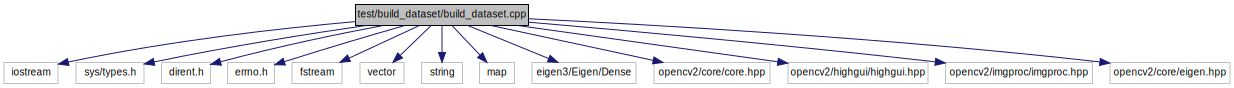
\includegraphics[width=350pt]{build__dataset_8cpp__incl}
\end{center}
\end{figure}
\subsection*{\-Typedefs}
\begin{DoxyCompactItemize}
\item 
typedef \-Eigen\-::\-Matrix$<$ uchar, \*
\-Dynamic, \-Dynamic $>$ \hyperlink{build__dataset_8cpp_a8096e93505cddac4cf99c2301883ab14}{\-Matrix\-Xc}
\item 
typedef map$<$ string, \-Mat $>$ \hyperlink{build__dataset_8cpp_a1761a0dff3537da3743c4d92ce94e5a9}{\-Src\-Img\-Map\-Type}
\item 
typedef map$<$ string, \-Vector\-Xf $>$ \hyperlink{build__dataset_8cpp_a2ad1d3d85356f042b317cde803b43667}{\-Src\-Depth\-Map\-Type}
\item 
typedef map$<$ string, \-Vector\-Xi $>$ \hyperlink{build__dataset_8cpp_a5332f8cbe4a18b3e5263613824a599ee}{\-Src\-Label\-Map\-Type}
\end{DoxyCompactItemize}
\subsection*{\-Functions}
\begin{DoxyCompactItemize}
\item 
void \hyperlink{build__dataset_8cpp_ad55cea6ce9e53c805e4fa88ffb179cec}{get\-Name\-List\-In\-File} (string path\-To\-File, vector$<$ string $>$ \&v\-Name\-List)
\item 
void \hyperlink{build__dataset_8cpp_aba3394f5f8d4e7581bc5ecbaaf0313b5}{build\-Image\-Subset} (string path\-To\-Image\-Dir, const vector$<$ string $>$ \&name\-List, vector$<$ vector$<$ \-Matrix\-Xi $>$ $>$ \&subset\-Img)
\item 
void \hyperlink{build__dataset_8cpp_a46e72f416948302d7a240c2384e9869b}{build\-Region\-Subset} (string path\-To\-Label\-Dir, const vector$<$ string $>$ \&name\-List, \-Vector\-Xi \&subset\-Label)
\item 
void \hyperlink{build__dataset_8cpp_a777e74a6234e94a8485bce69b1b6630e}{merge\-Vectors} (const vector$<$ \-Vector\-Xi $>$ \&src, \-Vector\-Xi \&dest)
\item 
void \hyperlink{build__dataset_8cpp_ac52bc11ce3cf73533b206f8afb6ae0d5}{build\-Image\-Set} (string path\-To\-Image\-Dir, const vector$<$ string $>$ \&v\-Name\-List\-Eval, const vector$<$ string $>$ \&v\-Name\-List\-Train, vector$<$ vector$<$ \-Matrix\-Xi $>$ $>$ \&img\-Set\-Eval, vector$<$ vector$<$ \-Matrix\-Xi $>$ $>$ \&img\-Set\-Train)
\item 
void \hyperlink{build__dataset_8cpp_a6524223e76c6cdcbb8abd8d231a2dae3}{build\-Region\-Set} (string path\-To\-Label\-Dir, const vector$<$ string $>$ \&v\-Name\-List\-Eval, const vector$<$ string $>$ \&v\-Name\-List\-Train, \-Vector\-Xi \&label\-Set\-Eval, \-Vector\-Xi \&label\-Set\-Train)
\item 
void \hyperlink{build__dataset_8cpp_a51008ea6d639927b35887511b24530a9}{build\-Data\-Set} (string base\-Path, vector$<$ vector$<$ \-Matrix\-Xi $>$ $>$ \&img\-Set\-Eval, vector$<$ string $>$ \&v\-Filename\-Eval, \-Vector\-Xi \&label\-Set\-Eval, vector$<$ vector$<$ \-Matrix\-Xi $>$ $>$ \&img\-Set\-Train, vector$<$ string $>$ \&v\-Filename\-Train, \-Vector\-Xi \&label\-Set\-Train)
\item 
void \hyperlink{build__dataset_8cpp_a2ac061736f98bb0c934b885d485b08f3}{convert\-Eig\-Yuv\-To\-Cv\-Bgr} (const vector$<$ \-Matrix\-Xi $>$ \&v\-Eig\-Yuv, \-Mat \&mat\-Bgr)
\item 
void \hyperlink{build__dataset_8cpp_a8662eeae70d4db4c23616897372daa41}{convert\-Label\-To\-Image} (const \-Vector\-Xi \&label, long pos, long length, \-Mat \&img)
\item 
void \hyperlink{build__dataset_8cpp_a97ee70a8770dc30d06c744b24eb2fcfc}{help} ()
\item 
int \hyperlink{build__dataset_8cpp_a3c04138a5bfe5d72780bb7e82a18e627}{main} (int argc, char $\ast$$\ast$argv)
\end{DoxyCompactItemize}


\subsection{\-Typedef \-Documentation}
\hypertarget{build__dataset_8cpp_a8096e93505cddac4cf99c2301883ab14}{\index{build\-\_\-dataset.\-cpp@{build\-\_\-dataset.\-cpp}!\-Matrix\-Xc@{\-Matrix\-Xc}}
\index{\-Matrix\-Xc@{\-Matrix\-Xc}!build_dataset.cpp@{build\-\_\-dataset.\-cpp}}
\subsubsection[{\-Matrix\-Xc}]{\setlength{\rightskip}{0pt plus 5cm}typedef \-Eigen\-::\-Matrix$<$uchar, \-Dynamic, \-Dynamic$>$ {\bf \-Matrix\-Xc}}}\label{build__dataset_8cpp_a8096e93505cddac4cf99c2301883ab14}
\hypertarget{build__dataset_8cpp_a2ad1d3d85356f042b317cde803b43667}{\index{build\-\_\-dataset.\-cpp@{build\-\_\-dataset.\-cpp}!\-Src\-Depth\-Map\-Type@{\-Src\-Depth\-Map\-Type}}
\index{\-Src\-Depth\-Map\-Type@{\-Src\-Depth\-Map\-Type}!build_dataset.cpp@{build\-\_\-dataset.\-cpp}}
\subsubsection[{\-Src\-Depth\-Map\-Type}]{\setlength{\rightskip}{0pt plus 5cm}typedef map$<$string,\-Vector\-Xf$>$ {\bf \-Src\-Depth\-Map\-Type}}}\label{build__dataset_8cpp_a2ad1d3d85356f042b317cde803b43667}
\hypertarget{build__dataset_8cpp_a1761a0dff3537da3743c4d92ce94e5a9}{\index{build\-\_\-dataset.\-cpp@{build\-\_\-dataset.\-cpp}!\-Src\-Img\-Map\-Type@{\-Src\-Img\-Map\-Type}}
\index{\-Src\-Img\-Map\-Type@{\-Src\-Img\-Map\-Type}!build_dataset.cpp@{build\-\_\-dataset.\-cpp}}
\subsubsection[{\-Src\-Img\-Map\-Type}]{\setlength{\rightskip}{0pt plus 5cm}typedef map$<$string,\-Mat$>$ {\bf \-Src\-Img\-Map\-Type}}}\label{build__dataset_8cpp_a1761a0dff3537da3743c4d92ce94e5a9}
\hypertarget{build__dataset_8cpp_a5332f8cbe4a18b3e5263613824a599ee}{\index{build\-\_\-dataset.\-cpp@{build\-\_\-dataset.\-cpp}!\-Src\-Label\-Map\-Type@{\-Src\-Label\-Map\-Type}}
\index{\-Src\-Label\-Map\-Type@{\-Src\-Label\-Map\-Type}!build_dataset.cpp@{build\-\_\-dataset.\-cpp}}
\subsubsection[{\-Src\-Label\-Map\-Type}]{\setlength{\rightskip}{0pt plus 5cm}typedef map$<$string,\-Vector\-Xi$>$ {\bf \-Src\-Label\-Map\-Type}}}\label{build__dataset_8cpp_a5332f8cbe4a18b3e5263613824a599ee}


\subsection{\-Function \-Documentation}
\hypertarget{build__dataset_8cpp_a51008ea6d639927b35887511b24530a9}{\index{build\-\_\-dataset.\-cpp@{build\-\_\-dataset.\-cpp}!build\-Data\-Set@{build\-Data\-Set}}
\index{build\-Data\-Set@{build\-Data\-Set}!build_dataset.cpp@{build\-\_\-dataset.\-cpp}}
\subsubsection[{build\-Data\-Set}]{\setlength{\rightskip}{0pt plus 5cm}void {\bf build\-Data\-Set} (
\begin{DoxyParamCaption}
\item[{string}]{base\-Path, }
\item[{vector$<$ vector$<$ \-Matrix\-Xi $>$ $>$ \&}]{img\-Set\-Eval, }
\item[{vector$<$ string $>$ \&}]{v\-Filename\-Eval, }
\item[{\-Vector\-Xi \&}]{label\-Set\-Eval, }
\item[{vector$<$ vector$<$ \-Matrix\-Xi $>$ $>$ \&}]{img\-Set\-Train, }
\item[{vector$<$ string $>$ \&}]{v\-Filename\-Train, }
\item[{\-Vector\-Xi \&}]{label\-Set\-Train}
\end{DoxyParamCaption}
)}}\label{build__dataset_8cpp_a51008ea6d639927b35887511b24530a9}


\-Here is the call graph for this function\-:
\nopagebreak
\begin{figure}[H]
\begin{center}
\leavevmode
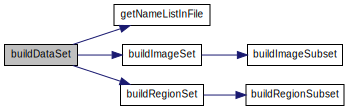
\includegraphics[width=350pt]{build__dataset_8cpp_a51008ea6d639927b35887511b24530a9_cgraph}
\end{center}
\end{figure}


\hypertarget{build__dataset_8cpp_ac52bc11ce3cf73533b206f8afb6ae0d5}{\index{build\-\_\-dataset.\-cpp@{build\-\_\-dataset.\-cpp}!build\-Image\-Set@{build\-Image\-Set}}
\index{build\-Image\-Set@{build\-Image\-Set}!build_dataset.cpp@{build\-\_\-dataset.\-cpp}}
\subsubsection[{build\-Image\-Set}]{\setlength{\rightskip}{0pt plus 5cm}void {\bf build\-Image\-Set} (
\begin{DoxyParamCaption}
\item[{string}]{path\-To\-Image\-Dir, }
\item[{const vector$<$ string $>$ \&}]{v\-Name\-List\-Eval, }
\item[{const vector$<$ string $>$ \&}]{v\-Name\-List\-Train, }
\item[{vector$<$ vector$<$ \-Matrix\-Xi $>$ $>$ \&}]{img\-Set\-Eval, }
\item[{vector$<$ vector$<$ \-Matrix\-Xi $>$ $>$ \&}]{img\-Set\-Train}
\end{DoxyParamCaption}
)}}\label{build__dataset_8cpp_ac52bc11ce3cf73533b206f8afb6ae0d5}


\-Here is the call graph for this function\-:
\nopagebreak
\begin{figure}[H]
\begin{center}
\leavevmode
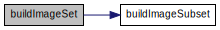
\includegraphics[width=292pt]{build__dataset_8cpp_ac52bc11ce3cf73533b206f8afb6ae0d5_cgraph}
\end{center}
\end{figure}


\hypertarget{build__dataset_8cpp_aba3394f5f8d4e7581bc5ecbaaf0313b5}{\index{build\-\_\-dataset.\-cpp@{build\-\_\-dataset.\-cpp}!build\-Image\-Subset@{build\-Image\-Subset}}
\index{build\-Image\-Subset@{build\-Image\-Subset}!build_dataset.cpp@{build\-\_\-dataset.\-cpp}}
\subsubsection[{build\-Image\-Subset}]{\setlength{\rightskip}{0pt plus 5cm}void {\bf build\-Image\-Subset} (
\begin{DoxyParamCaption}
\item[{string}]{path\-To\-Image\-Dir, }
\item[{const vector$<$ string $>$ \&}]{name\-List, }
\item[{vector$<$ vector$<$ \-Matrix\-Xi $>$ $>$ \&}]{subset\-Img}
\end{DoxyParamCaption}
)}}\label{build__dataset_8cpp_aba3394f5f8d4e7581bc5ecbaaf0313b5}
\hypertarget{build__dataset_8cpp_a6524223e76c6cdcbb8abd8d231a2dae3}{\index{build\-\_\-dataset.\-cpp@{build\-\_\-dataset.\-cpp}!build\-Region\-Set@{build\-Region\-Set}}
\index{build\-Region\-Set@{build\-Region\-Set}!build_dataset.cpp@{build\-\_\-dataset.\-cpp}}
\subsubsection[{build\-Region\-Set}]{\setlength{\rightskip}{0pt plus 5cm}void {\bf build\-Region\-Set} (
\begin{DoxyParamCaption}
\item[{string}]{path\-To\-Label\-Dir, }
\item[{const vector$<$ string $>$ \&}]{v\-Name\-List\-Eval, }
\item[{const vector$<$ string $>$ \&}]{v\-Name\-List\-Train, }
\item[{\-Vector\-Xi \&}]{label\-Set\-Eval, }
\item[{\-Vector\-Xi \&}]{label\-Set\-Train}
\end{DoxyParamCaption}
)}}\label{build__dataset_8cpp_a6524223e76c6cdcbb8abd8d231a2dae3}


\-Here is the call graph for this function\-:
\nopagebreak
\begin{figure}[H]
\begin{center}
\leavevmode
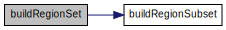
\includegraphics[width=298pt]{build__dataset_8cpp_a6524223e76c6cdcbb8abd8d231a2dae3_cgraph}
\end{center}
\end{figure}


\hypertarget{build__dataset_8cpp_a46e72f416948302d7a240c2384e9869b}{\index{build\-\_\-dataset.\-cpp@{build\-\_\-dataset.\-cpp}!build\-Region\-Subset@{build\-Region\-Subset}}
\index{build\-Region\-Subset@{build\-Region\-Subset}!build_dataset.cpp@{build\-\_\-dataset.\-cpp}}
\subsubsection[{build\-Region\-Subset}]{\setlength{\rightskip}{0pt plus 5cm}void {\bf build\-Region\-Subset} (
\begin{DoxyParamCaption}
\item[{string}]{path\-To\-Label\-Dir, }
\item[{const vector$<$ string $>$ \&}]{name\-List, }
\item[{\-Vector\-Xi \&}]{subset\-Label}
\end{DoxyParamCaption}
)}}\label{build__dataset_8cpp_a46e72f416948302d7a240c2384e9869b}
\hypertarget{build__dataset_8cpp_a2ac061736f98bb0c934b885d485b08f3}{\index{build\-\_\-dataset.\-cpp@{build\-\_\-dataset.\-cpp}!convert\-Eig\-Yuv\-To\-Cv\-Bgr@{convert\-Eig\-Yuv\-To\-Cv\-Bgr}}
\index{convert\-Eig\-Yuv\-To\-Cv\-Bgr@{convert\-Eig\-Yuv\-To\-Cv\-Bgr}!build_dataset.cpp@{build\-\_\-dataset.\-cpp}}
\subsubsection[{convert\-Eig\-Yuv\-To\-Cv\-Bgr}]{\setlength{\rightskip}{0pt plus 5cm}void {\bf convert\-Eig\-Yuv\-To\-Cv\-Bgr} (
\begin{DoxyParamCaption}
\item[{const vector$<$ \-Matrix\-Xi $>$ \&}]{v\-Eig\-Yuv, }
\item[{\-Mat \&}]{mat\-Bgr}
\end{DoxyParamCaption}
)}}\label{build__dataset_8cpp_a2ac061736f98bb0c934b885d485b08f3}
\hypertarget{build__dataset_8cpp_a8662eeae70d4db4c23616897372daa41}{\index{build\-\_\-dataset.\-cpp@{build\-\_\-dataset.\-cpp}!convert\-Label\-To\-Image@{convert\-Label\-To\-Image}}
\index{convert\-Label\-To\-Image@{convert\-Label\-To\-Image}!build_dataset.cpp@{build\-\_\-dataset.\-cpp}}
\subsubsection[{convert\-Label\-To\-Image}]{\setlength{\rightskip}{0pt plus 5cm}void {\bf convert\-Label\-To\-Image} (
\begin{DoxyParamCaption}
\item[{const \-Vector\-Xi \&}]{label, }
\item[{long}]{pos, }
\item[{long}]{length, }
\item[{\-Mat \&}]{img}
\end{DoxyParamCaption}
)}}\label{build__dataset_8cpp_a8662eeae70d4db4c23616897372daa41}
\hypertarget{build__dataset_8cpp_ad55cea6ce9e53c805e4fa88ffb179cec}{\index{build\-\_\-dataset.\-cpp@{build\-\_\-dataset.\-cpp}!get\-Name\-List\-In\-File@{get\-Name\-List\-In\-File}}
\index{get\-Name\-List\-In\-File@{get\-Name\-List\-In\-File}!build_dataset.cpp@{build\-\_\-dataset.\-cpp}}
\subsubsection[{get\-Name\-List\-In\-File}]{\setlength{\rightskip}{0pt plus 5cm}void {\bf get\-Name\-List\-In\-File} (
\begin{DoxyParamCaption}
\item[{string}]{path\-To\-File, }
\item[{vector$<$ string $>$ \&}]{v\-Name\-List}
\end{DoxyParamCaption}
)}}\label{build__dataset_8cpp_ad55cea6ce9e53c805e4fa88ffb179cec}
\hypertarget{build__dataset_8cpp_a97ee70a8770dc30d06c744b24eb2fcfc}{\index{build\-\_\-dataset.\-cpp@{build\-\_\-dataset.\-cpp}!help@{help}}
\index{help@{help}!build_dataset.cpp@{build\-\_\-dataset.\-cpp}}
\subsubsection[{help}]{\setlength{\rightskip}{0pt plus 5cm}void {\bf help} (
\begin{DoxyParamCaption}
{}
\end{DoxyParamCaption}
)}}\label{build__dataset_8cpp_a97ee70a8770dc30d06c744b24eb2fcfc}
\hypertarget{build__dataset_8cpp_a3c04138a5bfe5d72780bb7e82a18e627}{\index{build\-\_\-dataset.\-cpp@{build\-\_\-dataset.\-cpp}!main@{main}}
\index{main@{main}!build_dataset.cpp@{build\-\_\-dataset.\-cpp}}
\subsubsection[{main}]{\setlength{\rightskip}{0pt plus 5cm}int {\bf main} (
\begin{DoxyParamCaption}
\item[{int}]{argc, }
\item[{char $\ast$$\ast$}]{argv}
\end{DoxyParamCaption}
)}}\label{build__dataset_8cpp_a3c04138a5bfe5d72780bb7e82a18e627}


\-Here is the call graph for this function\-:
\nopagebreak
\begin{figure}[H]
\begin{center}
\leavevmode
\includegraphics[width=350pt]{build__dataset_8cpp_a3c04138a5bfe5d72780bb7e82a18e627_cgraph}
\end{center}
\end{figure}


\hypertarget{build__dataset_8cpp_a777e74a6234e94a8485bce69b1b6630e}{\index{build\-\_\-dataset.\-cpp@{build\-\_\-dataset.\-cpp}!merge\-Vectors@{merge\-Vectors}}
\index{merge\-Vectors@{merge\-Vectors}!build_dataset.cpp@{build\-\_\-dataset.\-cpp}}
\subsubsection[{merge\-Vectors}]{\setlength{\rightskip}{0pt plus 5cm}void {\bf merge\-Vectors} (
\begin{DoxyParamCaption}
\item[{const vector$<$ \-Vector\-Xi $>$ \&}]{src, }
\item[{\-Vector\-Xi \&}]{dest}
\end{DoxyParamCaption}
)}}\label{build__dataset_8cpp_a777e74a6234e94a8485bce69b1b6630e}

\input{conv2d_8cpp}
\input{sigmoid_8cpp}
\hypertarget{test__util__fun_8cpp}{\section{test/test\-\_\-util\-\_\-fun.cpp \-File \-Reference}
\label{test__util__fun_8cpp}\index{test/test\-\_\-util\-\_\-fun.\-cpp@{test/test\-\_\-util\-\_\-fun.\-cpp}}
}
{\ttfamily \#include $<$iostream$>$}\*
{\ttfamily \#include $<$gtest/gtest.\-h$>$}\*
{\ttfamily \#include $<$\-Eigen/\-Dense$>$}\*
{\ttfamily \#include $<$vector$>$}\*
{\ttfamily \#include \char`\"{}conv\-\_\-layer.\-h\char`\"{}}\*
\-Include dependency graph for test\-\_\-util\-\_\-fun.\-cpp\-:
\nopagebreak
\begin{figure}[H]
\begin{center}
\leavevmode
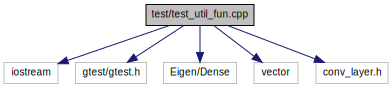
\includegraphics[width=350pt]{test__util__fun_8cpp__incl}
\end{center}
\end{figure}
\subsection*{\-Functions}
\begin{DoxyCompactItemize}
\item 
\hyperlink{test__util__fun_8cpp_ab1e233885020f733f92df828651171aa}{\-T\-E\-S\-T} (\-Sigmoid\-Test, \-Assertion\-Near)
\item 
\hyperlink{test__util__fun_8cpp_a661af029c7daf92822bade12583be80a}{\-T\-E\-S\-T} (\-Get\-Feature\-Vector\-Test, \-Assertion\-Equal)
\item 
int \hyperlink{test__util__fun_8cpp_a3c04138a5bfe5d72780bb7e82a18e627}{main} (int argc, char $\ast$$\ast$argv)
\end{DoxyCompactItemize}


\subsection{\-Function \-Documentation}
\hypertarget{test__util__fun_8cpp_a3c04138a5bfe5d72780bb7e82a18e627}{\index{test\-\_\-util\-\_\-fun.\-cpp@{test\-\_\-util\-\_\-fun.\-cpp}!main@{main}}
\index{main@{main}!test_util_fun.cpp@{test\-\_\-util\-\_\-fun.\-cpp}}
\subsubsection[{main}]{\setlength{\rightskip}{0pt plus 5cm}int {\bf main} (
\begin{DoxyParamCaption}
\item[{int}]{argc, }
\item[{char $\ast$$\ast$}]{argv}
\end{DoxyParamCaption}
)}}\label{test__util__fun_8cpp_a3c04138a5bfe5d72780bb7e82a18e627}
\hypertarget{test__util__fun_8cpp_ab1e233885020f733f92df828651171aa}{\index{test\-\_\-util\-\_\-fun.\-cpp@{test\-\_\-util\-\_\-fun.\-cpp}!\-T\-E\-S\-T@{\-T\-E\-S\-T}}
\index{\-T\-E\-S\-T@{\-T\-E\-S\-T}!test_util_fun.cpp@{test\-\_\-util\-\_\-fun.\-cpp}}
\subsubsection[{\-T\-E\-S\-T}]{\setlength{\rightskip}{0pt plus 5cm}{\bf \-T\-E\-S\-T} (
\begin{DoxyParamCaption}
\item[{\-Sigmoid\-Test}]{, }
\item[{\-Assertion\-Near}]{}
\end{DoxyParamCaption}
)}}\label{test__util__fun_8cpp_ab1e233885020f733f92df828651171aa}


\-Here is the call graph for this function\-:
\nopagebreak
\begin{figure}[H]
\begin{center}
\leavevmode
\includegraphics[width=240pt]{test__util__fun_8cpp_ab1e233885020f733f92df828651171aa_cgraph}
\end{center}
\end{figure}


\hypertarget{test__util__fun_8cpp_a661af029c7daf92822bade12583be80a}{\index{test\-\_\-util\-\_\-fun.\-cpp@{test\-\_\-util\-\_\-fun.\-cpp}!\-T\-E\-S\-T@{\-T\-E\-S\-T}}
\index{\-T\-E\-S\-T@{\-T\-E\-S\-T}!test_util_fun.cpp@{test\-\_\-util\-\_\-fun.\-cpp}}
\subsubsection[{\-T\-E\-S\-T}]{\setlength{\rightskip}{0pt plus 5cm}{\bf \-T\-E\-S\-T} (
\begin{DoxyParamCaption}
\item[{\-Get\-Feature\-Vector\-Test}]{, }
\item[{\-Assertion\-Equal}]{}
\end{DoxyParamCaption}
)}}\label{test__util__fun_8cpp_a661af029c7daf92822bade12583be80a}


\-Here is the call graph for this function\-:
\nopagebreak
\begin{figure}[H]
\begin{center}
\leavevmode
\includegraphics[width=288pt]{test__util__fun_8cpp_a661af029c7daf92822bade12583be80a_cgraph}
\end{center}
\end{figure}



\hypertarget{test_2yaml__t__load_8cpp}{\section{test/yaml\-\_\-t\-\_\-load.cpp \-File \-Reference}
\label{test_2yaml__t__load_8cpp}\index{test/yaml\-\_\-t\-\_\-load.\-cpp@{test/yaml\-\_\-t\-\_\-load.\-cpp}}
}
{\ttfamily \#include $<$iostream$>$}\*
{\ttfamily \#include $<$fstream$>$}\*
{\ttfamily \#include \char`\"{}yaml-\/cpp/yaml.\-h\char`\"{}}\*
{\ttfamily \#include $<$\-Eigen/\-Dense$>$}\*
{\ttfamily \#include $<$stdlib.\-h$>$}\*
{\ttfamily \#include $<$string$>$}\*
{\ttfamily \#include $<$string.\-h$>$}\*
\-Include dependency graph for yaml\-\_\-t\-\_\-load.\-cpp\-:
\nopagebreak
\begin{figure}[H]
\begin{center}
\leavevmode
\includegraphics[width=350pt]{test_2yaml__t__load_8cpp__incl}
\end{center}
\end{figure}
\subsection*{\-Functions}
\begin{DoxyCompactItemize}
\item 
\-Matrix\-Xd \hyperlink{test_2yaml__t__load_8cpp_a600eac78667d5a813045d8ef2f4395dd}{d} (3, 3)
\item 
\-Vector\-Xi \hyperlink{test_2yaml__t__load_8cpp_a80d599bd22867a8e610e0be09bf1128d}{v} (3)
\item 
void \hyperlink{test_2yaml__t__load_8cpp_a15e6c82d14b7cde034d53e566fd2ff8e}{parser\-\_\-yaml\-\_\-para} (string \&\hyperlink{yaml__t__load_8cpp_a7f01c047eb310166e695d4232ebd1fae}{dir}, \-Matrix\-Xd \&\hyperlink{yaml__t__load_8cpp_a600eac78667d5a813045d8ef2f4395dd}{d}, int \&\hyperlink{yaml__t__load_8cpp_a62c66ce2f11b397011ce5d92cc33f6c0}{\-Label\-\_\-number}, \-Vector\-Xi \&\hyperlink{yaml__t__load_8cpp_a80d599bd22867a8e610e0be09bf1128d}{v}, double \&\hyperlink{yaml__t__load_8cpp_acb484cd30430928d888abe1cfda0d9bb}{w\-\_\-bound}, double \&\hyperlink{yaml__t__load_8cpp_a674b759c775a81169ae20a20b4b2f4db}{b\-\_\-bound}, double \&\hyperlink{yaml__t__load_8cpp_a7b45f711c59e30b2aa59c4c954ad8ea1}{learning\-\_\-rate})
\item 
int \hyperlink{test_2yaml__t__load_8cpp_a0ddf1224851353fc92bfbff6f499fa97}{main} (int argc, char $\ast$argv\mbox{[}$\,$\mbox{]})
\end{DoxyCompactItemize}
\subsection*{\-Variables}
\begin{DoxyCompactItemize}
\item 
string \hyperlink{test_2yaml__t__load_8cpp_a7f01c047eb310166e695d4232ebd1fae}{dir} = \char`\"{}../seq.\-yaml\char`\"{}
\item 
int \hyperlink{test_2yaml__t__load_8cpp_a62c66ce2f11b397011ce5d92cc33f6c0}{\-Label\-\_\-number}
\item 
double \hyperlink{test_2yaml__t__load_8cpp_acb484cd30430928d888abe1cfda0d9bb}{w\-\_\-bound}
\item 
double \hyperlink{test_2yaml__t__load_8cpp_a674b759c775a81169ae20a20b4b2f4db}{b\-\_\-bound}
\item 
double \hyperlink{test_2yaml__t__load_8cpp_a7b45f711c59e30b2aa59c4c954ad8ea1}{learning\-\_\-rate}
\end{DoxyCompactItemize}


\subsection{\-Function \-Documentation}
\hypertarget{test_2yaml__t__load_8cpp_a600eac78667d5a813045d8ef2f4395dd}{\index{test/yaml\-\_\-t\-\_\-load.\-cpp@{test/yaml\-\_\-t\-\_\-load.\-cpp}!d@{d}}
\index{d@{d}!test/yaml_t_load.cpp@{test/yaml\-\_\-t\-\_\-load.\-cpp}}
\subsubsection[{d}]{\setlength{\rightskip}{0pt plus 5cm}\-Matrix\-Xd {\bf d} (
\begin{DoxyParamCaption}
\item[{3}]{, }
\item[{3}]{}
\end{DoxyParamCaption}
)}}\label{test_2yaml__t__load_8cpp_a600eac78667d5a813045d8ef2f4395dd}
\hypertarget{test_2yaml__t__load_8cpp_a0ddf1224851353fc92bfbff6f499fa97}{\index{test/yaml\-\_\-t\-\_\-load.\-cpp@{test/yaml\-\_\-t\-\_\-load.\-cpp}!main@{main}}
\index{main@{main}!test/yaml_t_load.cpp@{test/yaml\-\_\-t\-\_\-load.\-cpp}}
\subsubsection[{main}]{\setlength{\rightskip}{0pt plus 5cm}int {\bf main} (
\begin{DoxyParamCaption}
\item[{int}]{argc, }
\item[{char $\ast$}]{argv\mbox{[}$\,$\mbox{]}}
\end{DoxyParamCaption}
)}}\label{test_2yaml__t__load_8cpp_a0ddf1224851353fc92bfbff6f499fa97}


\-Here is the call graph for this function\-:
\nopagebreak
\begin{figure}[H]
\begin{center}
\leavevmode
\includegraphics[width=314pt]{test_2yaml__t__load_8cpp_a0ddf1224851353fc92bfbff6f499fa97_cgraph}
\end{center}
\end{figure}


\hypertarget{test_2yaml__t__load_8cpp_a15e6c82d14b7cde034d53e566fd2ff8e}{\index{test/yaml\-\_\-t\-\_\-load.\-cpp@{test/yaml\-\_\-t\-\_\-load.\-cpp}!parser\-\_\-yaml\-\_\-para@{parser\-\_\-yaml\-\_\-para}}
\index{parser\-\_\-yaml\-\_\-para@{parser\-\_\-yaml\-\_\-para}!test/yaml_t_load.cpp@{test/yaml\-\_\-t\-\_\-load.\-cpp}}
\subsubsection[{parser\-\_\-yaml\-\_\-para}]{\setlength{\rightskip}{0pt plus 5cm}void {\bf parser\-\_\-yaml\-\_\-para} (
\begin{DoxyParamCaption}
\item[{string \&}]{dir, }
\item[{\-Matrix\-Xd \&}]{d, }
\item[{int \&}]{\-Label\-\_\-number, }
\item[{\-Vector\-Xi \&}]{v, }
\item[{double \&}]{w\-\_\-bound, }
\item[{double \&}]{b\-\_\-bound, }
\item[{double \&}]{learning\-\_\-rate}
\end{DoxyParamCaption}
)}}\label{test_2yaml__t__load_8cpp_a15e6c82d14b7cde034d53e566fd2ff8e}


\-Here is the call graph for this function\-:
\nopagebreak
\begin{figure}[H]
\begin{center}
\leavevmode
\includegraphics[width=240pt]{test_2yaml__t__load_8cpp_a15e6c82d14b7cde034d53e566fd2ff8e_cgraph}
\end{center}
\end{figure}


\hypertarget{test_2yaml__t__load_8cpp_a80d599bd22867a8e610e0be09bf1128d}{\index{test/yaml\-\_\-t\-\_\-load.\-cpp@{test/yaml\-\_\-t\-\_\-load.\-cpp}!v@{v}}
\index{v@{v}!test/yaml_t_load.cpp@{test/yaml\-\_\-t\-\_\-load.\-cpp}}
\subsubsection[{v}]{\setlength{\rightskip}{0pt plus 5cm}\-Vector\-Xi {\bf v} (
\begin{DoxyParamCaption}
\item[{3}]{}
\end{DoxyParamCaption}
)}}\label{test_2yaml__t__load_8cpp_a80d599bd22867a8e610e0be09bf1128d}


\subsection{\-Variable \-Documentation}
\hypertarget{test_2yaml__t__load_8cpp_a674b759c775a81169ae20a20b4b2f4db}{\index{test/yaml\-\_\-t\-\_\-load.\-cpp@{test/yaml\-\_\-t\-\_\-load.\-cpp}!b\-\_\-bound@{b\-\_\-bound}}
\index{b\-\_\-bound@{b\-\_\-bound}!test/yaml_t_load.cpp@{test/yaml\-\_\-t\-\_\-load.\-cpp}}
\subsubsection[{b\-\_\-bound}]{\setlength{\rightskip}{0pt plus 5cm}double {\bf b\-\_\-bound}}}\label{test_2yaml__t__load_8cpp_a674b759c775a81169ae20a20b4b2f4db}
\hypertarget{test_2yaml__t__load_8cpp_a7f01c047eb310166e695d4232ebd1fae}{\index{test/yaml\-\_\-t\-\_\-load.\-cpp@{test/yaml\-\_\-t\-\_\-load.\-cpp}!dir@{dir}}
\index{dir@{dir}!test/yaml_t_load.cpp@{test/yaml\-\_\-t\-\_\-load.\-cpp}}
\subsubsection[{dir}]{\setlength{\rightskip}{0pt plus 5cm}string {\bf dir} = \char`\"{}../seq.\-yaml\char`\"{}}}\label{test_2yaml__t__load_8cpp_a7f01c047eb310166e695d4232ebd1fae}
\hypertarget{test_2yaml__t__load_8cpp_a62c66ce2f11b397011ce5d92cc33f6c0}{\index{test/yaml\-\_\-t\-\_\-load.\-cpp@{test/yaml\-\_\-t\-\_\-load.\-cpp}!\-Label\-\_\-number@{\-Label\-\_\-number}}
\index{\-Label\-\_\-number@{\-Label\-\_\-number}!test/yaml_t_load.cpp@{test/yaml\-\_\-t\-\_\-load.\-cpp}}
\subsubsection[{\-Label\-\_\-number}]{\setlength{\rightskip}{0pt plus 5cm}int {\bf \-Label\-\_\-number}}}\label{test_2yaml__t__load_8cpp_a62c66ce2f11b397011ce5d92cc33f6c0}
\hypertarget{test_2yaml__t__load_8cpp_a7b45f711c59e30b2aa59c4c954ad8ea1}{\index{test/yaml\-\_\-t\-\_\-load.\-cpp@{test/yaml\-\_\-t\-\_\-load.\-cpp}!learning\-\_\-rate@{learning\-\_\-rate}}
\index{learning\-\_\-rate@{learning\-\_\-rate}!test/yaml_t_load.cpp@{test/yaml\-\_\-t\-\_\-load.\-cpp}}
\subsubsection[{learning\-\_\-rate}]{\setlength{\rightskip}{0pt plus 5cm}double {\bf learning\-\_\-rate}}}\label{test_2yaml__t__load_8cpp_a7b45f711c59e30b2aa59c4c954ad8ea1}
\hypertarget{test_2yaml__t__load_8cpp_acb484cd30430928d888abe1cfda0d9bb}{\index{test/yaml\-\_\-t\-\_\-load.\-cpp@{test/yaml\-\_\-t\-\_\-load.\-cpp}!w\-\_\-bound@{w\-\_\-bound}}
\index{w\-\_\-bound@{w\-\_\-bound}!test/yaml_t_load.cpp@{test/yaml\-\_\-t\-\_\-load.\-cpp}}
\subsubsection[{w\-\_\-bound}]{\setlength{\rightskip}{0pt plus 5cm}double {\bf w\-\_\-bound}}}\label{test_2yaml__t__load_8cpp_acb484cd30430928d888abe1cfda0d9bb}

\input{yaml__t__load_8cpp}
\input{test_2yaml__test_8cpp}
\input{yaml__test_8cpp}
\printindex
\end{document}
